\documentclass[12pt,openany]{book}
%---------------------------------------Packages---------------------------------------


\usepackage[paper=a4paper]{geometry} %,left=32mm,right=32mm,top=30mm,bottom=30mm
\usepackage[ngerman,english]{babel}
\usepackage{fancyhdr}
\usepackage[utf8]{inputenc}
% \usepackage{lmodern} % Font normal
% \usepackage{tgpagella} % Font palantino
\usepackage[T1]{fontenc}
\usepackage[rgb,dvipsnames]{xcolor}
\usepackage{microtype}
\usepackage[all]{nowidow}
\usepackage{graphicx}
\usepackage{float}
%\usepackage{tikz}
\usepackage{pgfplots}
\usepackage[shortlabels]{enumitem}
\usepackage{amsmath}
\usepackage{amssymb}
\usepackage{amsthm}
\usepackage{siunitx}
\usepackage{booktabs}
\usepackage{mathtools}
\usepackage{wrapfig}
\usepackage[titletoc]{appendix}
\usepackage[nonewpage,quiet]{imakeidx}
\usepackage[linktoc=all]{hyperref}
\usepackage{tocloft}
\usepackage{titlesec}
\usepackage[labelsep=period]{caption}
\usepackage{subcaption}
\usepackage[style=numeric,maxnames=3,sortcites=true,doi=false,isbn=false,eprint=false,url=false]{biblatex}
\usepackage[nameinlink,capitalize]{cleveref}
\usepackage{csquotes}
\usepackage{thmtools} 
\usepackage{xurl}
\usepackage{grffile}
\usepackage{mdframed} %vorher war [framemethod=TikZ]
\usepackage{algorithm}
\usepackage{algpseudocode}
% \usepackage{printlen}
% \usepackage{layouts} # only used to get \textwidth



%---------------------------------------Diverse Befehle---------------------------------------


\addbibresource{Bibliography.bib}
\graphicspath{{./figures/}}
\setlist{nosep} %enumitem: remove vertical spaces around lists


\DeclareCaptionLabelSeparator{bar}{\,|\, }
\captionsetup{font=small,labelfont=bf, labelsep=bar, width=.9\linewidth,belowskip=-7pt}


\numberwithin{equation}{chapter} %gleichungen in kapiteln nummerieren
\allowdisplaybreaks % align umgebungen umbrechen
\setlength{\oddsidemargin}{35pt} 
\setlength{\evensidemargin}{35pt}%macht, dass gerade und ungerade seiten gleiche margins haben
\pgfplotsset{compat=1.18}
\usepgfplotslibrary{external} 
\tikzexternalize

\indexsetup{level=\section,noclearpage,firstpagestyle=fancy}
\makeindex[columns=2, title=Alphabetical Index]


\setcounter{topnumber}{1} %max number of floats at the top of a page
% \makeindex[columns=3, title=Alphabetical Index]


% % Diese Befehle ändern die Farben der Seitennummern
% % im Inhaltsverzeichnis. Möglich durch \usepackage{tocloft}
% \makeatletter
% % \definecolor{bluelinkcolor}{RGB}{35, 60, 138}
% \renewcommand{\cftchappagefont}{\bfseries\color{BlueViolet}}
% \renewcommand{\cftsecpagefont}{\color{BlueViolet}}
% \let\cftsubsecpagefont\cftsecpagefont % \renewcommand{\cftsubsecpagefont}{\HyColor@HyperrefColor{red}\@linkcolor}
% \makeatother




%---------------------------------------Cleverref---------------------------------------



\crefname{chapter}{Chapter}{Chapters}
\crefname{section}{Section}{Sections}
\crefname{subsection}{Subsection}{Subsections}
\crefname{algorithm}{Algorithm}{Algorithms}
\crefname{figure}{Figure}{Figures}
\crefname{table}{Table}{Tables}
\crefname{equation}{Equation}{Equations}
\crefname{problem}{Problem}{Problems}
\crefname{appchap}{Appendix}{Appendices}
\crefname{appsec}{Appendix}{Appendices}



%---------------------------------------PDF Einstellungen---------------------------------------



\hypersetup{
  pdftitle    = {Bachelorarbeit},
  pdfsubject  = {Chance of Further Improvement in Bayesian Optimization},
  pdfauthor   = {Marc Philip Kaebel},
  colorlinks  = false,
  pdfborder   = {0 0 0}
}



%---------------------------------------Clickable Chapter Names leading to TOC------------------



\AtBeginDocument{
  \let\oldchapter\chapter
  \RenewDocumentCommand{\chapter}{s o m}{%
    \clearpage
    \IfBooleanTF{#1}
    {\oldchapter*{\hyperref[toc]{#3}}}% \chapter*[..]{...}
    {\IfValueTF{#2}
      {\oldchapter[#2]{\hyperref[toc]{#3}}}% \chapter[..]{...}
      {\oldchapter[#3]{\hyperref[toc]{#3}}}% \chapter{...}
      \label{chapter-\thechapter}% \label this chapter
    }%
  }
}

%---------------------------------------Fancy Pagestyle Setup-----------------------------------

\setlength{\headheight}{15pt} %fancyhdr

\fancypagestyle{plain}{  % makes the first pages of chapters have page numbers that are at the bottom on the sides
\fancyhf{}
\fancyfoot[LE,RO]{\textbf{\thepage}}
\renewcommand{\headrulewidth}{0pt}
\renewcommand{\footrulewidth}{0pt}}




\pagestyle{fancy}
\renewcommand{\chaptermark}[1]{\markboth{#1}{}}
%\renewcommand{\sectionmark}[1]{\markright{#1}}
\fancyhf{}
%\fancyhead[LE,RO]{\thepage}
\fancyhead[LE]{\nouppercase{\scshape\textbf{\thepage}\,|\, \leftmark}}
\fancyhead[RO]{\nouppercase{\scshape\rightmark\, |\,\textbf{\thepage}}}
\renewcommand{\headrulewidth}{0pt}



%---------------------------------------Chapter and Section Style-------------------------------




\titleformat{\subsection}
{\normalfont\itshape\large}
{\thesection}{0.5em}{\normalfont\normalsize\itshape}
% {\thesection\,|\, }{0.5em}{}




\titleformat{\section}
{\normalfont\bfseries\large}
{\thesection}{0.5em}{\normalfont\normalsize\scshape}
% {\thesection\,|\, }{0.5em}{}



\titleformat{\chapter}[display]
  {\normalfont}{\large\scshape\chaptertitlename\ \thechapter}{0pt}{\LARGE\bfseries}
% \titlespacing*{\chapter}s
%   {0pt}{65pt}{40pt}



%---------------------------------------Thmtools---------------------------------------



\let\proof\relax
\let\endproof\relax



\declaretheoremstyle[
spaceabove=3pt, 
spacebelow=6pt,
headfont=\normalfont\bfseries,
notefont=\mdseries, 
notebraces={(}{)},
bodyfont=\normalfont]{standardthm}

\declaretheoremstyle[
spaceabove=3pt, 
spacebelow=6pt,
headfont=\normalfont\bfseries,%\scshape,
notefont=\normalfont\mdseries, 
notebraces={(}{)},
bodyfont=\normalfont,
postheadspace=1em]{standarddef}

\declaretheoremstyle[
spaceabove=0pt, 
spacebelow=0pt,
headfont=\normalfont\bfseries,
notefont=\mdseries, 
notebraces={(}{)},
bodyfont=\normalfont,
postheadspace=1em]{standardrem}

\declaretheoremstyle[
spaceabove=0pt, 
spacebelow=0pt,
headfont=\normalfont\bfseries,
bodyfont=\normalfont,
postheadspace=1em,
qed=\qedsymbol%$\blacksquare$
]{standardproof}



\declaretheorem[
style=standardthm,
refname={Theorem,Theorems},
Refname={Theorem,Theorems},
numberwithin=chapter]{theorem}

\declaretheorem[
style=standardthm,
sibling=theorem,
refname={Proposition,Propositions},
Refname={Proposition,Propositions}]{proposition}

\declaretheorem[
style=standardthm,
sibling=theorem,
refname={Lemma,Lemmas},
Refname={Lemma,Lemmas}]{lemma}

\declaretheorem[
style=standardthm,
sibling=theorem,
refname={Corollary,Corollaries},
Refname={Corollary,Corollaries}]{corollary}



\declaretheorem[
style=standarddef,
sibling=theorem,
refname={Definition,Definitions},
Refname={Definition,Definitions}]{definition}

\declaretheorem[
style=standarddef,
sibling=theorem,
refname={Example,Examples},
Refname={Example,Examples}]{example}

\declaretheorem[
style=standardrem,
sibling=theorem,
refname={Remark,Remarks},
Refname={Remark,Remarks}]{remark}



\declaretheorem[
style=standardproof,
unnumbered,
refname={Proof,Proofs},
Refname={Proof,Proofs}]{proof}



%------------------------------------------------------------------------------
%---------------------------------------Diverse Operatoren----------------------------


\newcommand{\limn}{\lim_{n \to \infty}}
\newcommand{\Id}{\mathrm{Id}}
\newcommand*{\dx}[1][x]{\,\mathrm{d} #1}
\newcommand{\Var}{\operatorname{Var}}
\newcommand{\Cov}{\operatorname{Cov}}
\renewcommand{\tilde}{\widetilde}
\renewcommand{\hat}{\widehat}
\DeclareMathOperator*{\argmax}{argmax} % Stern bedeutet hier, dass _ Argumente unter dem Wort stehen wie bei limits
\DeclareMathOperator*{\argmin}{argmin}
\DeclareMathOperator*{\E}{E}
\DeclareMathOperator{\diam}{diam}
\newcommand{\Prob}{\mathrm{P}}



















%---------------------------------------No longer in use------------------------------


%\newcommand{\einhalb}{\frac{1}{2}}
%\newcommand{\teinhalb}{\tfrac{1}{2}}
%\newcommand{\halbe}[1]{\frac{#1}{2}}
%\newcommand{\norm}[1]{\Vert #1 \Vert}
%\newcommand{\scalednorm}[1]{\left\Vert #1 \right\Vert}
%\newcommand{\scal}[2]{\langle #1, #2 \rangle}
%\newcommand{\einsdurch}[1]{\frac{1}{#1}}
%\newcommand{\teinsdurch}[1]{\tfrac{1}{#1}}
%\newcommand{\R}{\mathbb{R}}
%\newcommand{\N}{\mathbb{N}}
%\newcommand{\Q}{\mathbb{Q}}
%\newcommand{\C}{\mathbb{C}}
%\newcommand{\Z}{\mathbb{Z}}
%\newcommand{\K}{\mathbb{K}}
%\newcommand{\E}{\mathbb{E}}
%\renewcommand{\P}{\mathbb{P}}
%\newcommand{\G}{\mathcal{G}}
%\newcommand{\Ha}{\mathcal{H}}
%\newcommand{\X}{\mathcal{X}}
%\newcommand{\F}{\mathcal{F}}
%\newcommand{\ohnenull}{\setminus\{0\}}
%\newcommand{\links}{\glqq$\Leftarrow$\grqq}
%\newcommand{\und}{~~ \text{and} ~~}
%\newcommand{\gdw}{\Leftrightarrow}
%\newcommand{\rot}{\color{red}}
%\newcommand{\blau}{\color{blue}}
%\newcommand{\partiell}[2]{\frac{\partial #1}{\partial #2}}
%\newcommand{\nhn}{\newline\hfill\newline}
%\newcommand{\inv}{^{-1}}
%\newcommand{\Prox}{\mathrm{Prox}}
%\newcommand{\ol}[1]{\overline{#1}}
%\newcommand{\eigs}{\Lambda}
%\newcommand{\Uad}{\mathcal{U}_{\mathrm{ad}}}
%\newcommand{\tran}[1]{#1^{\mathsf{T}}}
%\newcommand{\tp}{^{\mathsf{T}}}
%\newcommand{\mtran}[1]{#1^{-\mathsf{T}}}
%\newcommand{\mtp}{^{-\mathsf{T}}}
%\newcommand{\herm}[1]{#1^{\mathsf{H}}}
%\newcommand{\hm}{^{\mathsf{H}}}
%\newcommand{\Pc}{\mathcal{P}_{\mathrm{c}}}
%\newcommand{\Pf}{\mathcal{P}_{\mathrm{f}}}
%\newcommand{\hatPc}{\hat{\mathcal{P}}_{\mathrm{c}}}
%\newcommand{\hatPf}{\hat{\mathcal{P}}_{\mathrm{f}}}
%\newcommand{\hatX}{\hat{X}}
%\newcommand{\hatY}{\hat{Y}}
%\newcommand{\Ac}{A_{\text{c}}}
%\newcommand{\Bc}{B_{\text{c}}}
%\newcommand{\Cc}{C_{\text{c}}}
%\newcommand{\hatAc}{\hat{A_{\text{c}}}}
%\newcommand{\hatBc}{\hat{B_{\text{c}}}}
%\newcommand{\hatCc}{\hat{C_{\text{c}}}}
%\newcommand{\tmp}{_{\text{tmp}}}
%\newcommand{\Atmp}{A\tmp}
%\newcommand{\Gtmp}{G\tmp}
%\newcommand{\Jtmp}{J\tmp}
%\newcommand{\hinf}{{\mathcal{H}_\infty}}
%\newcommand{\dgap}{\delta_{\text{gap}}}
%\newcommand{\ddgap}{\overset{\to}{\dgap}}
%\renewcommand{\l}{\left}
%\newcommand{\m}{\middle}
%\renewcommand{\r}{\right}
%\renewcommand{\Re}{\textrm{Re}}

%---------------------------------------Tweaks---------------------------------------



% eqref shortcut
%\let\oldeqref\eqref
%\renewcommand{\eqref}[1]{\oldeqref{eq:#1}}




%------------------------------------------------------------------------------




\title{Bachelor Thesis}
\author{Marc Philip Kaebel}
\date{\today}



\begin{document}



\frontmatter


\begin{titlepage}
    \begin{center}
        % \textcolor{red}{Dateiname: Abschlussarbeit\_381256.pdf}\\
        \vspace*{3cm}
        \Large
        Bachelor Thesis\\
        \vspace{0.6cm} 
        \LARGE
        \textbf{Estimates on the Chance of Further Improvement in Bayesian Optimization}\\
        \vspace{5cm}
        \large
        \begin{tabular}{ll}
        Author: & Marc Philip Kaebel (381256) \\
        Supervisor: & Prof. Dr. Hanno Gottschalk \\
        Co-Supervisor: & Dr. Tobias Riedlinger \\
        \end{tabular}
        
        \vspace{0.6cm}     
        % \normalsize
        Technische Universität Berlin \\
        Fakultät II \\
        Institut für Mathematik \\
        \vfill    
        %\vspace{0.8cm}            
        \the\year{}
    \end{center}
 \end{titlepage}
\pagestyle{empty}
% \hfill\newpage


\setcounter{page}{1}
% \clearpage
% \phantomsection
% \addcontentsline{toc}{chapter}{Eidesstattliche Versicherung}
% \chapter*{Eidesstattliche Versicherung}
% \markboth{Eidesstattliche Versicherung}{Eidesstattliche Versicherung}

\chapter*{Eidesstattliche Versicherung}


\begin{otherlanguage}{ngerman}
Hiermit erkläre ich, dass ich die vorliegende Arbeit selbstständig und eigenhändig sowie ohne unerlaubte
fremde Hilfe und ausschließlich unter Verwendung der aufgeführten Quellen und Hilfsmittel angefertigt habe. \\
\hphantom{t} \\
\hphantom{t} \\
\hphantom{t} \\
Berlin, den 21.03.2024 \\  % date
\\
\hphantom{hallo} \hfill Marc Philip Kaebel \\
\hphantom{hallo} \hfill {\small Matrikelnummer: 381256}
\end{otherlanguage}

%\newpage
%\hfill \newpage

\chapter*{Kurzzusammenfassung}
\begin{otherlanguage}{ngerman}
%\addcontentsline{toc}{chapter}{Kurzzusammenfassung}
In dieser Arbeit beschäftigen wir uns mit dem Bayesian Optimization Verfahren. 
% \textcolor{red}{Anders? Bayesian Optimization ist ein Verfahren, das ...}
Dazu legen wir zunächst einige Grundlagen aus der Wahrscheinlichkeitstheorie. 
Wir leiten die Gaussian Process Regression her und zeigen einige ihrer bekannten Eigenschaften. 
Anschließend erkären wir, was Bayesian Optimization ist und leiten eine obere Schranke für die Wahrscheinlichkeit einer weiteren Verbesserung her. 
Mithilfe dieser Abschätzung schlagen wir eine Erweiterung der Bayesian Optimization vor, die auf dem Branch and Bound Algorithmus basiert. 
\end{otherlanguage}





\newpage
\phantomsection
\tableofcontents\label{toc}
\addtocontents{toc}{\protect\thispagestyle{empty}}

% \mainmatter

\makeatletter % this removes the empty page after the first chapter (which is created because first pages always are on the right side usually)
\@twosidefalse
\mainmatter
\@twosidetrue
\makeatother

\pagestyle{fancy}






\chapter{Introduction}\label{chap:intro}
% This thesis is about Bayesian optimization. The main topic is the derivation of an upper bound on the chance of further improvement in such a scheme.
% \textcolor{red}{Satz rauslassen?}
% % In order to discuss Bayesian optimization, the first half of this thesis will be dedicated to the neccessary probability theory foundations, some stochastical tools and Gaussian process regression.
%
%
\section{Topic of this Thesis}
% \section*{Optimization}
Let us start by looking at a generic optimization problem. That is, we have some function \( f \colon \mathcal{X} \to \mathbb{R} \) on a suitable space $\mathcal{X}$, and we want to find a minimizer
\[
    x^{*} \in \argmin_{x \in \mathcal{X}} f(x).
\]
An example of such a function is shown in \cref{fig:optimization_intro}.
One simple way to approach this problem would be to start checking points randomly and remembering the lowest point we encountered. 
For finite spaces $\mathcal{X}$ this is sometimes feasible, but quickly runs into limitations if the number of elements gets too large.
% 
An example of a more refined strategy would be to use information of a lower bound on the function, if we have one. 
This lets us rule out areas of search, where the lower bound is already higher than a value we have previously encountered, and subsequently only look in areas, in which improvement is possible. 
This method is called branch and bound~\cite{lawler1966branch}.
Although this is an improvement on the previous method, it still does not guarantee, that we will find the global minimum.
% 
But it does show a common theme in optimization of using all the availaible information about the space and the objective function to our benefit. Is the function differentiable? Linear? Is the space discrete? Is it continous, but still finite dimensional? These, among many others, are restrictions with specific approaches taylored to them. The approach discussed in this thesis is no different. 
\begin{figure}[H]
    \centering
    %% Creator: Matplotlib, PGF backend
%%
%% To include the figure in your LaTeX document, write
%%   \input{<filename>.pgf}
%%
%% Make sure the required packages are loaded in your preamble
%%   \usepackage{pgf}
%%
%% Also ensure that all the required font packages are loaded; for instance,
%% the lmodern package is sometimes necessary when using math font.
%%   \usepackage{lmodern}
%%
%% Figures using additional raster images can only be included by \input if
%% they are in the same directory as the main LaTeX file. For loading figures
%% from other directories you can use the `import` package
%%   \usepackage{import}
%%
%% and then include the figures with
%%   \import{<path to file>}{<filename>.pgf}
%%
%% Matplotlib used the following preamble
%%   \def\mathdefault#1{#1}
%%   \everymath=\expandafter{\the\everymath\displaystyle}
%%   \usepackage[T1]{fontenc}
%%   \usepackage{siunitx}
%%   \usepackage{amssymb}
%%   \usepackage{amsmath}
%%   \makeatletter\@ifpackageloaded{underscore}{}{\usepackage[strings]{underscore}}\makeatother
%%
\begingroup%
\makeatletter%
\begin{pgfpicture}%
\pgfpathrectangle{\pgfpointorigin}{\pgfqpoint{3.473106in}{1.287899in}}%
\pgfusepath{use as bounding box, clip}%
\begin{pgfscope}%
\pgfsetbuttcap%
\pgfsetmiterjoin%
\definecolor{currentfill}{rgb}{1.000000,1.000000,1.000000}%
\pgfsetfillcolor{currentfill}%
\pgfsetlinewidth{0.000000pt}%
\definecolor{currentstroke}{rgb}{1.000000,1.000000,1.000000}%
\pgfsetstrokecolor{currentstroke}%
\pgfsetdash{}{0pt}%
\pgfpathmoveto{\pgfqpoint{0.000000in}{0.000000in}}%
\pgfpathlineto{\pgfqpoint{3.473106in}{0.000000in}}%
\pgfpathlineto{\pgfqpoint{3.473106in}{1.287899in}}%
\pgfpathlineto{\pgfqpoint{0.000000in}{1.287899in}}%
\pgfpathlineto{\pgfqpoint{0.000000in}{0.000000in}}%
\pgfpathclose%
\pgfusepath{fill}%
\end{pgfscope}%
\begin{pgfscope}%
\pgfsetbuttcap%
\pgfsetmiterjoin%
\definecolor{currentfill}{rgb}{1.000000,1.000000,1.000000}%
\pgfsetfillcolor{currentfill}%
\pgfsetlinewidth{0.000000pt}%
\definecolor{currentstroke}{rgb}{0.000000,0.000000,0.000000}%
\pgfsetstrokecolor{currentstroke}%
\pgfsetstrokeopacity{0.000000}%
\pgfsetdash{}{0pt}%
\pgfpathmoveto{\pgfqpoint{0.000000in}{0.000000in}}%
\pgfpathlineto{\pgfqpoint{3.473106in}{0.000000in}}%
\pgfpathlineto{\pgfqpoint{3.473106in}{1.287899in}}%
\pgfpathlineto{\pgfqpoint{0.000000in}{1.287899in}}%
\pgfpathlineto{\pgfqpoint{0.000000in}{0.000000in}}%
\pgfpathclose%
\pgfusepath{fill}%
\end{pgfscope}%
\begin{pgfscope}%
\pgfpathrectangle{\pgfqpoint{0.000000in}{0.000000in}}{\pgfqpoint{3.473106in}{1.287899in}}%
\pgfusepath{clip}%
\pgfsetrectcap%
\pgfsetroundjoin%
\pgfsetlinewidth{1.505625pt}%
\definecolor{currentstroke}{rgb}{0.149020,0.274510,0.325490}%
\pgfsetstrokecolor{currentstroke}%
\pgfsetdash{}{0pt}%
\pgfpathmoveto{\pgfqpoint{0.157868in}{1.229358in}}%
\pgfpathlineto{\pgfqpoint{0.192634in}{1.146241in}}%
\pgfpathlineto{\pgfqpoint{0.284290in}{0.923314in}}%
\pgfpathlineto{\pgfqpoint{0.309574in}{0.869211in}}%
\pgfpathlineto{\pgfqpoint{0.331698in}{0.827275in}}%
\pgfpathlineto{\pgfqpoint{0.350661in}{0.796130in}}%
\pgfpathlineto{\pgfqpoint{0.366463in}{0.773921in}}%
\pgfpathlineto{\pgfqpoint{0.382266in}{0.755307in}}%
\pgfpathlineto{\pgfqpoint{0.398069in}{0.740370in}}%
\pgfpathlineto{\pgfqpoint{0.410711in}{0.731066in}}%
\pgfpathlineto{\pgfqpoint{0.423353in}{0.724062in}}%
\pgfpathlineto{\pgfqpoint{0.435995in}{0.719272in}}%
\pgfpathlineto{\pgfqpoint{0.448637in}{0.716573in}}%
\pgfpathlineto{\pgfqpoint{0.461279in}{0.715806in}}%
\pgfpathlineto{\pgfqpoint{0.477082in}{0.717276in}}%
\pgfpathlineto{\pgfqpoint{0.492885in}{0.721038in}}%
\pgfpathlineto{\pgfqpoint{0.511848in}{0.727896in}}%
\pgfpathlineto{\pgfqpoint{0.540293in}{0.741053in}}%
\pgfpathlineto{\pgfqpoint{0.581379in}{0.760196in}}%
\pgfpathlineto{\pgfqpoint{0.600343in}{0.766790in}}%
\pgfpathlineto{\pgfqpoint{0.616145in}{0.770350in}}%
\pgfpathlineto{\pgfqpoint{0.631948in}{0.771715in}}%
\pgfpathlineto{\pgfqpoint{0.647751in}{0.770543in}}%
\pgfpathlineto{\pgfqpoint{0.660393in}{0.767599in}}%
\pgfpathlineto{\pgfqpoint{0.673035in}{0.762761in}}%
\pgfpathlineto{\pgfqpoint{0.685677in}{0.755963in}}%
\pgfpathlineto{\pgfqpoint{0.701480in}{0.744666in}}%
\pgfpathlineto{\pgfqpoint{0.717282in}{0.730274in}}%
\pgfpathlineto{\pgfqpoint{0.733085in}{0.712880in}}%
\pgfpathlineto{\pgfqpoint{0.752048in}{0.688289in}}%
\pgfpathlineto{\pgfqpoint{0.771011in}{0.660049in}}%
\pgfpathlineto{\pgfqpoint{0.793135in}{0.623229in}}%
\pgfpathlineto{\pgfqpoint{0.821580in}{0.571392in}}%
\pgfpathlineto{\pgfqpoint{0.919556in}{0.388475in}}%
\pgfpathlineto{\pgfqpoint{0.941680in}{0.353405in}}%
\pgfpathlineto{\pgfqpoint{0.960643in}{0.326811in}}%
\pgfpathlineto{\pgfqpoint{0.979606in}{0.303867in}}%
\pgfpathlineto{\pgfqpoint{0.995409in}{0.287760in}}%
\pgfpathlineto{\pgfqpoint{1.011211in}{0.274520in}}%
\pgfpathlineto{\pgfqpoint{1.027014in}{0.264204in}}%
\pgfpathlineto{\pgfqpoint{1.042817in}{0.256815in}}%
\pgfpathlineto{\pgfqpoint{1.058619in}{0.252299in}}%
\pgfpathlineto{\pgfqpoint{1.074422in}{0.250554in}}%
\pgfpathlineto{\pgfqpoint{1.090225in}{0.251429in}}%
\pgfpathlineto{\pgfqpoint{1.106027in}{0.254731in}}%
\pgfpathlineto{\pgfqpoint{1.121830in}{0.260230in}}%
\pgfpathlineto{\pgfqpoint{1.140793in}{0.269362in}}%
\pgfpathlineto{\pgfqpoint{1.162917in}{0.282879in}}%
\pgfpathlineto{\pgfqpoint{1.188201in}{0.301065in}}%
\pgfpathlineto{\pgfqpoint{1.235609in}{0.338645in}}%
\pgfpathlineto{\pgfqpoint{1.273535in}{0.367359in}}%
\pgfpathlineto{\pgfqpoint{1.298820in}{0.383805in}}%
\pgfpathlineto{\pgfqpoint{1.320943in}{0.395585in}}%
\pgfpathlineto{\pgfqpoint{1.339907in}{0.403361in}}%
\pgfpathlineto{\pgfqpoint{1.358870in}{0.408754in}}%
\pgfpathlineto{\pgfqpoint{1.377833in}{0.411603in}}%
\pgfpathlineto{\pgfqpoint{1.396796in}{0.411814in}}%
\pgfpathlineto{\pgfqpoint{1.415759in}{0.409359in}}%
\pgfpathlineto{\pgfqpoint{1.434722in}{0.404268in}}%
\pgfpathlineto{\pgfqpoint{1.453686in}{0.396630in}}%
\pgfpathlineto{\pgfqpoint{1.472649in}{0.386584in}}%
\pgfpathlineto{\pgfqpoint{1.494772in}{0.372066in}}%
\pgfpathlineto{\pgfqpoint{1.516896in}{0.354877in}}%
\pgfpathlineto{\pgfqpoint{1.542180in}{0.332492in}}%
\pgfpathlineto{\pgfqpoint{1.573786in}{0.301394in}}%
\pgfpathlineto{\pgfqpoint{1.621194in}{0.251141in}}%
\pgfpathlineto{\pgfqpoint{1.684404in}{0.184594in}}%
\pgfpathlineto{\pgfqpoint{1.719170in}{0.151406in}}%
\pgfpathlineto{\pgfqpoint{1.747615in}{0.127241in}}%
\pgfpathlineto{\pgfqpoint{1.772899in}{0.108492in}}%
\pgfpathlineto{\pgfqpoint{1.798183in}{0.092604in}}%
\pgfpathlineto{\pgfqpoint{1.820307in}{0.081199in}}%
\pgfpathlineto{\pgfqpoint{1.842431in}{0.072201in}}%
\pgfpathlineto{\pgfqpoint{1.864554in}{0.065634in}}%
\pgfpathlineto{\pgfqpoint{1.886678in}{0.061478in}}%
\pgfpathlineto{\pgfqpoint{1.908802in}{0.059673in}}%
\pgfpathlineto{\pgfqpoint{1.930926in}{0.060123in}}%
\pgfpathlineto{\pgfqpoint{1.953049in}{0.062704in}}%
\pgfpathlineto{\pgfqpoint{1.978334in}{0.068069in}}%
\pgfpathlineto{\pgfqpoint{2.003618in}{0.075765in}}%
\pgfpathlineto{\pgfqpoint{2.032063in}{0.086862in}}%
\pgfpathlineto{\pgfqpoint{2.063668in}{0.101726in}}%
\pgfpathlineto{\pgfqpoint{2.101594in}{0.122286in}}%
\pgfpathlineto{\pgfqpoint{2.149002in}{0.150729in}}%
\pgfpathlineto{\pgfqpoint{2.300708in}{0.243785in}}%
\pgfpathlineto{\pgfqpoint{2.344955in}{0.267469in}}%
\pgfpathlineto{\pgfqpoint{2.386042in}{0.287079in}}%
\pgfpathlineto{\pgfqpoint{2.427129in}{0.304173in}}%
\pgfpathlineto{\pgfqpoint{2.465055in}{0.317652in}}%
\pgfpathlineto{\pgfqpoint{2.502981in}{0.328947in}}%
\pgfpathlineto{\pgfqpoint{2.544068in}{0.338828in}}%
\pgfpathlineto{\pgfqpoint{2.585155in}{0.346438in}}%
\pgfpathlineto{\pgfqpoint{2.629403in}{0.352362in}}%
\pgfpathlineto{\pgfqpoint{2.676811in}{0.356459in}}%
\pgfpathlineto{\pgfqpoint{2.730540in}{0.358815in}}%
\pgfpathlineto{\pgfqpoint{2.793750in}{0.359274in}}%
\pgfpathlineto{\pgfqpoint{2.879084in}{0.357480in}}%
\pgfpathlineto{\pgfqpoint{3.106643in}{0.351596in}}%
\pgfpathlineto{\pgfqpoint{3.191977in}{0.352227in}}%
\pgfpathlineto{\pgfqpoint{3.270990in}{0.355022in}}%
\pgfpathlineto{\pgfqpoint{3.315238in}{0.357581in}}%
\pgfpathlineto{\pgfqpoint{3.315238in}{0.357581in}}%
\pgfusepath{stroke}%
\end{pgfscope}%
\begin{pgfscope}%
\pgfpathrectangle{\pgfqpoint{0.000000in}{0.000000in}}{\pgfqpoint{3.473106in}{1.287899in}}%
\pgfusepath{clip}%
\pgfsetbuttcap%
\pgfsetroundjoin%
\pgfsetlinewidth{0.501875pt}%
\definecolor{currentstroke}{rgb}{0.000000,0.000000,0.000000}%
\pgfsetstrokecolor{currentstroke}%
\pgfsetdash{{1.850000pt}{0.800000pt}}{0.000000pt}%
\pgfpathmoveto{\pgfqpoint{1.911962in}{0.058541in}}%
\pgfpathlineto{\pgfqpoint{1.911962in}{1.117788in}}%
\pgfusepath{stroke}%
\end{pgfscope}%
\begin{pgfscope}%
\pgfpathrectangle{\pgfqpoint{0.000000in}{0.000000in}}{\pgfqpoint{3.473106in}{1.287899in}}%
\pgfusepath{clip}%
\pgfsetbuttcap%
\pgfsetroundjoin%
\definecolor{currentfill}{rgb}{0.000000,0.000000,0.000000}%
\pgfsetfillcolor{currentfill}%
\pgfsetlinewidth{1.003750pt}%
\definecolor{currentstroke}{rgb}{0.000000,0.000000,0.000000}%
\pgfsetstrokecolor{currentstroke}%
\pgfsetdash{}{0pt}%
\pgfsys@defobject{currentmarker}{\pgfqpoint{0.000000in}{-0.041667in}}{\pgfqpoint{0.000000in}{0.041667in}}{%
\pgfpathmoveto{\pgfqpoint{0.000000in}{-0.041667in}}%
\pgfpathlineto{\pgfqpoint{0.000000in}{0.041667in}}%
\pgfusepath{stroke,fill}%
}%
\begin{pgfscope}%
\pgfsys@transformshift{1.911962in}{1.117788in}%
\pgfsys@useobject{currentmarker}{}%
\end{pgfscope}%
\end{pgfscope}%
\begin{pgfscope}%
\pgfpathrectangle{\pgfqpoint{0.000000in}{0.000000in}}{\pgfqpoint{3.473106in}{1.287899in}}%
\pgfusepath{clip}%
\pgfsetbuttcap%
\pgfsetroundjoin%
\pgfsetlinewidth{0.501875pt}%
\definecolor{currentstroke}{rgb}{0.000000,0.000000,0.000000}%
\pgfsetstrokecolor{currentstroke}%
\pgfsetdash{{1.850000pt}{0.800000pt}}{0.000000pt}%
\pgfpathmoveto{\pgfqpoint{1.911962in}{0.058541in}}%
\pgfpathlineto{\pgfqpoint{0.508687in}{0.058541in}}%
\pgfusepath{stroke}%
\end{pgfscope}%
\begin{pgfscope}%
\pgfpathrectangle{\pgfqpoint{0.000000in}{0.000000in}}{\pgfqpoint{3.473106in}{1.287899in}}%
\pgfusepath{clip}%
\pgfsetbuttcap%
\pgfsetroundjoin%
\definecolor{currentfill}{rgb}{0.000000,0.000000,0.000000}%
\pgfsetfillcolor{currentfill}%
\pgfsetlinewidth{1.003750pt}%
\definecolor{currentstroke}{rgb}{0.000000,0.000000,0.000000}%
\pgfsetstrokecolor{currentstroke}%
\pgfsetdash{}{0pt}%
\pgfsys@defobject{currentmarker}{\pgfqpoint{-0.041667in}{-0.000000in}}{\pgfqpoint{0.041667in}{0.000000in}}{%
\pgfpathmoveto{\pgfqpoint{0.041667in}{-0.000000in}}%
\pgfpathlineto{\pgfqpoint{-0.041667in}{0.000000in}}%
\pgfusepath{stroke,fill}%
}%
\begin{pgfscope}%
\pgfsys@transformshift{0.508687in}{0.058541in}%
\pgfsys@useobject{currentmarker}{}%
\end{pgfscope}%
\end{pgfscope}%
\begin{pgfscope}%
\definecolor{textcolor}{rgb}{0.000000,0.000000,0.000000}%
\pgfsetstrokecolor{textcolor}%
\pgfsetfillcolor{textcolor}%
\pgftext[x=1.933012in,y=1.237836in,,]{\color{textcolor}{\rmfamily\fontsize{10.000000}{12.000000}\selectfont\catcode`\^=\active\def^{\ifmmode\sp\else\^{}\fi}\catcode`\%=\active\def%{\%}$x^*$}}%
\end{pgfscope}%
\begin{pgfscope}%
\definecolor{textcolor}{rgb}{0.000000,0.000000,0.000000}%
\pgfsetstrokecolor{textcolor}%
\pgfsetfillcolor{textcolor}%
\pgftext[x=0.368360in,y=0.058541in,,]{\color{textcolor}{\rmfamily\fontsize{10.000000}{12.000000}\selectfont\catcode`\^=\active\def^{\ifmmode\sp\else\^{}\fi}\catcode`\%=\active\def%{\%}$f^*$}}%
\end{pgfscope}%
\end{pgfpicture}%
\makeatother%
\endgroup%

    \caption{A first optimization example.}
    \label{fig:optimization_intro}
\end{figure}


The setup is as follows: We have a function that is possibly expensive to evaluate and behaves randomly, but the structure of that randomness can be well quantified locally.
``Structure of randomness?'' This is most easily explained with a picture. 
The data for the three pictures in \cref{fig:random_fields_intro.png} was randomly generated by three different random processes. 
They are all random, but don't share the same structure.
One could generate many pictures from the first process resembling the first picture in structure, but none would look like any, that were created by the second or third process.
A small spoiler of \cref{sec:random_fields} reveals that the difference in structure is determined by how much points in space are influenced by their neighboring points. 

\begin{figure}[b]
    \centering
    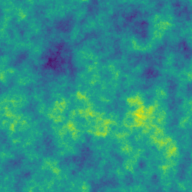
\includegraphics[scale=0.71]{random_field_matern_l_100_n_05-img0.png}
    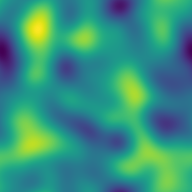
\includegraphics[scale=0.71]{random_field_matern_l_100_n_100-img0.png}
    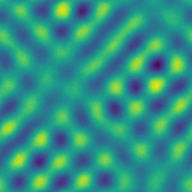
\includegraphics[scale=0.71]{random_field_cos_l_1000-img0.png}
    \caption{Samples drawn from random fields with three different covariance functions.}
    \label{fig:random_fields_intro.png}
\end{figure}








\subsection*{Gaussian Process Regression}
Say we now have a random process to model the structure of our optimization problem, more specifically a Gaussian process. It is characterized by a mean and covariance function quantifying the random structure. 
Possible realizations of such a process are shown in \cref{fig:sausage_plot_prior_matern}.
In Bayesian terms, this model is the prior, so the likelihood of samples before incorporating any measurement data.
How do we ensure, that the random process meets the measured values at the points of observation? 
For those points, how do we make it not random?
This is where the regression framework comes in. 
We can construct another random process, one that is an optimal predictor of the underlying process, conditional on the measured values.
It is constructed as a weighted linear combination of the measured values, with a covariance function that becomes zero at points of measurement. 
In Bayesian terms, this is the posterior.
In this way we can frame our beliefs as a prior distribution and update our model by conditioning on observations, thus arriving at a posterior distribution like \cref{fig:sausage_plot_posterior_matern}. 
This model is often referred to as a surrogate model.
One benefit of choosing Gaussian processes is that such a construction is then also a Gaussian process. 

% For a brief practical review of Bayesian statistics, we refer to~\cite{fornacon2022understanding}. \textcolor{red}{Maybe I leave out this last sentence.}

\begin{figure}[t]
    \centering
    %% Creator: Matplotlib, PGF backend
%%
%% To include the figure in your LaTeX document, write
%%   \input{<filename>.pgf}
%%
%% Make sure the required packages are loaded in your preamble
%%   \usepackage{pgf}
%%
%% Also ensure that all the required font packages are loaded; for instance,
%% the lmodern package is sometimes necessary when using math font.
%%   \usepackage{lmodern}
%%
%% Figures using additional raster images can only be included by \input if
%% they are in the same directory as the main LaTeX file. For loading figures
%% from other directories you can use the `import` package
%%   \usepackage{import}
%%
%% and then include the figures with
%%   \import{<path to file>}{<filename>.pgf}
%%
%% Matplotlib used the following preamble
%%   \def\mathdefault#1{#1}
%%   \everymath=\expandafter{\the\everymath\displaystyle}
%%   \usepackage[T1]{fontenc}
%%   \usepackage{siunitx}
%%   \usepackage{amssymb}
%%   \usepackage{amsmath}
%%   \makeatletter\@ifpackageloaded{underscore}{}{\usepackage[strings]{underscore}}\makeatother
%%
\begingroup%
\makeatletter%
\begin{pgfpicture}%
\pgfpathrectangle{\pgfpointorigin}{\pgfqpoint{5.788510in}{1.000000in}}%
\pgfusepath{use as bounding box, clip}%
\begin{pgfscope}%
\pgfsetbuttcap%
\pgfsetmiterjoin%
\definecolor{currentfill}{rgb}{1.000000,1.000000,1.000000}%
\pgfsetfillcolor{currentfill}%
\pgfsetlinewidth{0.000000pt}%
\definecolor{currentstroke}{rgb}{1.000000,1.000000,1.000000}%
\pgfsetstrokecolor{currentstroke}%
\pgfsetdash{}{0pt}%
\pgfpathmoveto{\pgfqpoint{0.000000in}{0.000000in}}%
\pgfpathlineto{\pgfqpoint{5.788510in}{0.000000in}}%
\pgfpathlineto{\pgfqpoint{5.788510in}{1.000000in}}%
\pgfpathlineto{\pgfqpoint{0.000000in}{1.000000in}}%
\pgfpathlineto{\pgfqpoint{0.000000in}{0.000000in}}%
\pgfpathclose%
\pgfusepath{fill}%
\end{pgfscope}%
\begin{pgfscope}%
\pgfsetbuttcap%
\pgfsetmiterjoin%
\definecolor{currentfill}{rgb}{1.000000,1.000000,1.000000}%
\pgfsetfillcolor{currentfill}%
\pgfsetlinewidth{0.000000pt}%
\definecolor{currentstroke}{rgb}{0.000000,0.000000,0.000000}%
\pgfsetstrokecolor{currentstroke}%
\pgfsetstrokeopacity{0.000000}%
\pgfsetdash{}{0pt}%
\pgfpathmoveto{\pgfqpoint{0.000000in}{0.000000in}}%
\pgfpathlineto{\pgfqpoint{5.788510in}{0.000000in}}%
\pgfpathlineto{\pgfqpoint{5.788510in}{0.800000in}}%
\pgfpathlineto{\pgfqpoint{0.000000in}{0.800000in}}%
\pgfpathlineto{\pgfqpoint{0.000000in}{0.000000in}}%
\pgfpathclose%
\pgfusepath{fill}%
\end{pgfscope}%
\begin{pgfscope}%
\pgfpathrectangle{\pgfqpoint{0.000000in}{0.000000in}}{\pgfqpoint{5.788510in}{0.800000in}}%
\pgfusepath{clip}%
\pgfsetbuttcap%
\pgfsetroundjoin%
\definecolor{currentfill}{rgb}{0.149020,0.274510,0.325490}%
\pgfsetfillcolor{currentfill}%
\pgfsetfillopacity{0.100000}%
\pgfsetlinewidth{1.003750pt}%
\definecolor{currentstroke}{rgb}{0.149020,0.274510,0.325490}%
\pgfsetstrokecolor{currentstroke}%
\pgfsetstrokeopacity{0.100000}%
\pgfsetdash{}{0pt}%
\pgfpathmoveto{\pgfqpoint{0.000000in}{0.723904in}}%
\pgfpathlineto{\pgfqpoint{0.000000in}{0.179224in}}%
\pgfpathlineto{\pgfqpoint{0.058470in}{0.179224in}}%
\pgfpathlineto{\pgfqpoint{0.116940in}{0.179224in}}%
\pgfpathlineto{\pgfqpoint{0.175409in}{0.179224in}}%
\pgfpathlineto{\pgfqpoint{0.233879in}{0.179224in}}%
\pgfpathlineto{\pgfqpoint{0.292349in}{0.179224in}}%
\pgfpathlineto{\pgfqpoint{0.350819in}{0.179224in}}%
\pgfpathlineto{\pgfqpoint{0.409289in}{0.179224in}}%
\pgfpathlineto{\pgfqpoint{0.467758in}{0.179224in}}%
\pgfpathlineto{\pgfqpoint{0.526228in}{0.179224in}}%
\pgfpathlineto{\pgfqpoint{0.584698in}{0.179224in}}%
\pgfpathlineto{\pgfqpoint{0.643168in}{0.179224in}}%
\pgfpathlineto{\pgfqpoint{0.701638in}{0.179224in}}%
\pgfpathlineto{\pgfqpoint{0.760107in}{0.179224in}}%
\pgfpathlineto{\pgfqpoint{0.818577in}{0.179224in}}%
\pgfpathlineto{\pgfqpoint{0.877047in}{0.179224in}}%
\pgfpathlineto{\pgfqpoint{0.935517in}{0.179224in}}%
\pgfpathlineto{\pgfqpoint{0.993987in}{0.179224in}}%
\pgfpathlineto{\pgfqpoint{1.052456in}{0.179224in}}%
\pgfpathlineto{\pgfqpoint{1.110926in}{0.179224in}}%
\pgfpathlineto{\pgfqpoint{1.169396in}{0.179224in}}%
\pgfpathlineto{\pgfqpoint{1.227866in}{0.179224in}}%
\pgfpathlineto{\pgfqpoint{1.286336in}{0.179224in}}%
\pgfpathlineto{\pgfqpoint{1.344805in}{0.179224in}}%
\pgfpathlineto{\pgfqpoint{1.403275in}{0.179224in}}%
\pgfpathlineto{\pgfqpoint{1.461745in}{0.179224in}}%
\pgfpathlineto{\pgfqpoint{1.520215in}{0.179224in}}%
\pgfpathlineto{\pgfqpoint{1.578685in}{0.179224in}}%
\pgfpathlineto{\pgfqpoint{1.637154in}{0.179224in}}%
\pgfpathlineto{\pgfqpoint{1.695624in}{0.179224in}}%
\pgfpathlineto{\pgfqpoint{1.754094in}{0.179224in}}%
\pgfpathlineto{\pgfqpoint{1.812564in}{0.179224in}}%
\pgfpathlineto{\pgfqpoint{1.871034in}{0.179224in}}%
\pgfpathlineto{\pgfqpoint{1.929503in}{0.179224in}}%
\pgfpathlineto{\pgfqpoint{1.987973in}{0.179224in}}%
\pgfpathlineto{\pgfqpoint{2.046443in}{0.179224in}}%
\pgfpathlineto{\pgfqpoint{2.104913in}{0.179224in}}%
\pgfpathlineto{\pgfqpoint{2.163383in}{0.179224in}}%
\pgfpathlineto{\pgfqpoint{2.221852in}{0.179224in}}%
\pgfpathlineto{\pgfqpoint{2.280322in}{0.179224in}}%
\pgfpathlineto{\pgfqpoint{2.338792in}{0.179224in}}%
\pgfpathlineto{\pgfqpoint{2.397262in}{0.179224in}}%
\pgfpathlineto{\pgfqpoint{2.455732in}{0.179224in}}%
\pgfpathlineto{\pgfqpoint{2.514201in}{0.179224in}}%
\pgfpathlineto{\pgfqpoint{2.572671in}{0.179224in}}%
\pgfpathlineto{\pgfqpoint{2.631141in}{0.179224in}}%
\pgfpathlineto{\pgfqpoint{2.689611in}{0.179224in}}%
\pgfpathlineto{\pgfqpoint{2.748081in}{0.179224in}}%
\pgfpathlineto{\pgfqpoint{2.806550in}{0.179224in}}%
\pgfpathlineto{\pgfqpoint{2.865020in}{0.179224in}}%
\pgfpathlineto{\pgfqpoint{2.923490in}{0.179224in}}%
\pgfpathlineto{\pgfqpoint{2.981960in}{0.179224in}}%
\pgfpathlineto{\pgfqpoint{3.040429in}{0.179224in}}%
\pgfpathlineto{\pgfqpoint{3.098899in}{0.179224in}}%
\pgfpathlineto{\pgfqpoint{3.157369in}{0.179224in}}%
\pgfpathlineto{\pgfqpoint{3.215839in}{0.179224in}}%
\pgfpathlineto{\pgfqpoint{3.274309in}{0.179224in}}%
\pgfpathlineto{\pgfqpoint{3.332778in}{0.179224in}}%
\pgfpathlineto{\pgfqpoint{3.391248in}{0.179224in}}%
\pgfpathlineto{\pgfqpoint{3.449718in}{0.179224in}}%
\pgfpathlineto{\pgfqpoint{3.508188in}{0.179224in}}%
\pgfpathlineto{\pgfqpoint{3.566658in}{0.179224in}}%
\pgfpathlineto{\pgfqpoint{3.625127in}{0.179224in}}%
\pgfpathlineto{\pgfqpoint{3.683597in}{0.179224in}}%
\pgfpathlineto{\pgfqpoint{3.742067in}{0.179224in}}%
\pgfpathlineto{\pgfqpoint{3.800537in}{0.179224in}}%
\pgfpathlineto{\pgfqpoint{3.859007in}{0.179224in}}%
\pgfpathlineto{\pgfqpoint{3.917476in}{0.179224in}}%
\pgfpathlineto{\pgfqpoint{3.975946in}{0.179224in}}%
\pgfpathlineto{\pgfqpoint{4.034416in}{0.179224in}}%
\pgfpathlineto{\pgfqpoint{4.092886in}{0.179224in}}%
\pgfpathlineto{\pgfqpoint{4.151356in}{0.179224in}}%
\pgfpathlineto{\pgfqpoint{4.209825in}{0.179224in}}%
\pgfpathlineto{\pgfqpoint{4.268295in}{0.179224in}}%
\pgfpathlineto{\pgfqpoint{4.326765in}{0.179224in}}%
\pgfpathlineto{\pgfqpoint{4.385235in}{0.179224in}}%
\pgfpathlineto{\pgfqpoint{4.443705in}{0.179224in}}%
\pgfpathlineto{\pgfqpoint{4.502174in}{0.179224in}}%
\pgfpathlineto{\pgfqpoint{4.560644in}{0.179224in}}%
\pgfpathlineto{\pgfqpoint{4.619114in}{0.179224in}}%
\pgfpathlineto{\pgfqpoint{4.677584in}{0.179224in}}%
\pgfpathlineto{\pgfqpoint{4.736054in}{0.179224in}}%
\pgfpathlineto{\pgfqpoint{4.794523in}{0.179224in}}%
\pgfpathlineto{\pgfqpoint{4.852993in}{0.179224in}}%
\pgfpathlineto{\pgfqpoint{4.911463in}{0.179224in}}%
\pgfpathlineto{\pgfqpoint{4.969933in}{0.179224in}}%
\pgfpathlineto{\pgfqpoint{5.028403in}{0.179224in}}%
\pgfpathlineto{\pgfqpoint{5.086872in}{0.179224in}}%
\pgfpathlineto{\pgfqpoint{5.145342in}{0.179224in}}%
\pgfpathlineto{\pgfqpoint{5.203812in}{0.179224in}}%
\pgfpathlineto{\pgfqpoint{5.262282in}{0.179224in}}%
\pgfpathlineto{\pgfqpoint{5.320752in}{0.179224in}}%
\pgfpathlineto{\pgfqpoint{5.379221in}{0.179224in}}%
\pgfpathlineto{\pgfqpoint{5.437691in}{0.179224in}}%
\pgfpathlineto{\pgfqpoint{5.496161in}{0.179224in}}%
\pgfpathlineto{\pgfqpoint{5.554631in}{0.179224in}}%
\pgfpathlineto{\pgfqpoint{5.613101in}{0.179224in}}%
\pgfpathlineto{\pgfqpoint{5.671570in}{0.179224in}}%
\pgfpathlineto{\pgfqpoint{5.730040in}{0.179224in}}%
\pgfpathlineto{\pgfqpoint{5.788510in}{0.179224in}}%
\pgfpathlineto{\pgfqpoint{5.788510in}{0.723904in}}%
\pgfpathlineto{\pgfqpoint{5.788510in}{0.723904in}}%
\pgfpathlineto{\pgfqpoint{5.730040in}{0.723904in}}%
\pgfpathlineto{\pgfqpoint{5.671570in}{0.723904in}}%
\pgfpathlineto{\pgfqpoint{5.613101in}{0.723904in}}%
\pgfpathlineto{\pgfqpoint{5.554631in}{0.723904in}}%
\pgfpathlineto{\pgfqpoint{5.496161in}{0.723904in}}%
\pgfpathlineto{\pgfqpoint{5.437691in}{0.723904in}}%
\pgfpathlineto{\pgfqpoint{5.379221in}{0.723904in}}%
\pgfpathlineto{\pgfqpoint{5.320752in}{0.723904in}}%
\pgfpathlineto{\pgfqpoint{5.262282in}{0.723904in}}%
\pgfpathlineto{\pgfqpoint{5.203812in}{0.723904in}}%
\pgfpathlineto{\pgfqpoint{5.145342in}{0.723904in}}%
\pgfpathlineto{\pgfqpoint{5.086872in}{0.723904in}}%
\pgfpathlineto{\pgfqpoint{5.028403in}{0.723904in}}%
\pgfpathlineto{\pgfqpoint{4.969933in}{0.723904in}}%
\pgfpathlineto{\pgfqpoint{4.911463in}{0.723904in}}%
\pgfpathlineto{\pgfqpoint{4.852993in}{0.723904in}}%
\pgfpathlineto{\pgfqpoint{4.794523in}{0.723904in}}%
\pgfpathlineto{\pgfqpoint{4.736054in}{0.723904in}}%
\pgfpathlineto{\pgfqpoint{4.677584in}{0.723904in}}%
\pgfpathlineto{\pgfqpoint{4.619114in}{0.723904in}}%
\pgfpathlineto{\pgfqpoint{4.560644in}{0.723904in}}%
\pgfpathlineto{\pgfqpoint{4.502174in}{0.723904in}}%
\pgfpathlineto{\pgfqpoint{4.443705in}{0.723904in}}%
\pgfpathlineto{\pgfqpoint{4.385235in}{0.723904in}}%
\pgfpathlineto{\pgfqpoint{4.326765in}{0.723904in}}%
\pgfpathlineto{\pgfqpoint{4.268295in}{0.723904in}}%
\pgfpathlineto{\pgfqpoint{4.209825in}{0.723904in}}%
\pgfpathlineto{\pgfqpoint{4.151356in}{0.723904in}}%
\pgfpathlineto{\pgfqpoint{4.092886in}{0.723904in}}%
\pgfpathlineto{\pgfqpoint{4.034416in}{0.723904in}}%
\pgfpathlineto{\pgfqpoint{3.975946in}{0.723904in}}%
\pgfpathlineto{\pgfqpoint{3.917476in}{0.723904in}}%
\pgfpathlineto{\pgfqpoint{3.859007in}{0.723904in}}%
\pgfpathlineto{\pgfqpoint{3.800537in}{0.723904in}}%
\pgfpathlineto{\pgfqpoint{3.742067in}{0.723904in}}%
\pgfpathlineto{\pgfqpoint{3.683597in}{0.723904in}}%
\pgfpathlineto{\pgfqpoint{3.625127in}{0.723904in}}%
\pgfpathlineto{\pgfqpoint{3.566658in}{0.723904in}}%
\pgfpathlineto{\pgfqpoint{3.508188in}{0.723904in}}%
\pgfpathlineto{\pgfqpoint{3.449718in}{0.723904in}}%
\pgfpathlineto{\pgfqpoint{3.391248in}{0.723904in}}%
\pgfpathlineto{\pgfqpoint{3.332778in}{0.723904in}}%
\pgfpathlineto{\pgfqpoint{3.274309in}{0.723904in}}%
\pgfpathlineto{\pgfqpoint{3.215839in}{0.723904in}}%
\pgfpathlineto{\pgfqpoint{3.157369in}{0.723904in}}%
\pgfpathlineto{\pgfqpoint{3.098899in}{0.723904in}}%
\pgfpathlineto{\pgfqpoint{3.040429in}{0.723904in}}%
\pgfpathlineto{\pgfqpoint{2.981960in}{0.723904in}}%
\pgfpathlineto{\pgfqpoint{2.923490in}{0.723904in}}%
\pgfpathlineto{\pgfqpoint{2.865020in}{0.723904in}}%
\pgfpathlineto{\pgfqpoint{2.806550in}{0.723904in}}%
\pgfpathlineto{\pgfqpoint{2.748081in}{0.723904in}}%
\pgfpathlineto{\pgfqpoint{2.689611in}{0.723904in}}%
\pgfpathlineto{\pgfqpoint{2.631141in}{0.723904in}}%
\pgfpathlineto{\pgfqpoint{2.572671in}{0.723904in}}%
\pgfpathlineto{\pgfqpoint{2.514201in}{0.723904in}}%
\pgfpathlineto{\pgfqpoint{2.455732in}{0.723904in}}%
\pgfpathlineto{\pgfqpoint{2.397262in}{0.723904in}}%
\pgfpathlineto{\pgfqpoint{2.338792in}{0.723904in}}%
\pgfpathlineto{\pgfqpoint{2.280322in}{0.723904in}}%
\pgfpathlineto{\pgfqpoint{2.221852in}{0.723904in}}%
\pgfpathlineto{\pgfqpoint{2.163383in}{0.723904in}}%
\pgfpathlineto{\pgfqpoint{2.104913in}{0.723904in}}%
\pgfpathlineto{\pgfqpoint{2.046443in}{0.723904in}}%
\pgfpathlineto{\pgfqpoint{1.987973in}{0.723904in}}%
\pgfpathlineto{\pgfqpoint{1.929503in}{0.723904in}}%
\pgfpathlineto{\pgfqpoint{1.871034in}{0.723904in}}%
\pgfpathlineto{\pgfqpoint{1.812564in}{0.723904in}}%
\pgfpathlineto{\pgfqpoint{1.754094in}{0.723904in}}%
\pgfpathlineto{\pgfqpoint{1.695624in}{0.723904in}}%
\pgfpathlineto{\pgfqpoint{1.637154in}{0.723904in}}%
\pgfpathlineto{\pgfqpoint{1.578685in}{0.723904in}}%
\pgfpathlineto{\pgfqpoint{1.520215in}{0.723904in}}%
\pgfpathlineto{\pgfqpoint{1.461745in}{0.723904in}}%
\pgfpathlineto{\pgfqpoint{1.403275in}{0.723904in}}%
\pgfpathlineto{\pgfqpoint{1.344805in}{0.723904in}}%
\pgfpathlineto{\pgfqpoint{1.286336in}{0.723904in}}%
\pgfpathlineto{\pgfqpoint{1.227866in}{0.723904in}}%
\pgfpathlineto{\pgfqpoint{1.169396in}{0.723904in}}%
\pgfpathlineto{\pgfqpoint{1.110926in}{0.723904in}}%
\pgfpathlineto{\pgfqpoint{1.052456in}{0.723904in}}%
\pgfpathlineto{\pgfqpoint{0.993987in}{0.723904in}}%
\pgfpathlineto{\pgfqpoint{0.935517in}{0.723904in}}%
\pgfpathlineto{\pgfqpoint{0.877047in}{0.723904in}}%
\pgfpathlineto{\pgfqpoint{0.818577in}{0.723904in}}%
\pgfpathlineto{\pgfqpoint{0.760107in}{0.723904in}}%
\pgfpathlineto{\pgfqpoint{0.701638in}{0.723904in}}%
\pgfpathlineto{\pgfqpoint{0.643168in}{0.723904in}}%
\pgfpathlineto{\pgfqpoint{0.584698in}{0.723904in}}%
\pgfpathlineto{\pgfqpoint{0.526228in}{0.723904in}}%
\pgfpathlineto{\pgfqpoint{0.467758in}{0.723904in}}%
\pgfpathlineto{\pgfqpoint{0.409289in}{0.723904in}}%
\pgfpathlineto{\pgfqpoint{0.350819in}{0.723904in}}%
\pgfpathlineto{\pgfqpoint{0.292349in}{0.723904in}}%
\pgfpathlineto{\pgfqpoint{0.233879in}{0.723904in}}%
\pgfpathlineto{\pgfqpoint{0.175409in}{0.723904in}}%
\pgfpathlineto{\pgfqpoint{0.116940in}{0.723904in}}%
\pgfpathlineto{\pgfqpoint{0.058470in}{0.723904in}}%
\pgfpathlineto{\pgfqpoint{0.000000in}{0.723904in}}%
\pgfpathlineto{\pgfqpoint{0.000000in}{0.723904in}}%
\pgfpathclose%
\pgfusepath{stroke,fill}%
\end{pgfscope}%
\begin{pgfscope}%
\pgfpathrectangle{\pgfqpoint{0.000000in}{0.000000in}}{\pgfqpoint{5.788510in}{0.800000in}}%
\pgfusepath{clip}%
\pgfsetrectcap%
\pgfsetroundjoin%
\pgfsetlinewidth{1.505625pt}%
\definecolor{currentstroke}{rgb}{1.000000,0.745098,0.043137}%
\pgfsetstrokecolor{currentstroke}%
\pgfsetdash{}{0pt}%
\pgfpathmoveto{\pgfqpoint{0.000000in}{0.036364in}}%
\pgfpathlineto{\pgfqpoint{0.058470in}{0.039774in}}%
\pgfpathlineto{\pgfqpoint{0.116940in}{0.044612in}}%
\pgfpathlineto{\pgfqpoint{0.175409in}{0.050882in}}%
\pgfpathlineto{\pgfqpoint{0.233879in}{0.058570in}}%
\pgfpathlineto{\pgfqpoint{0.292349in}{0.067642in}}%
\pgfpathlineto{\pgfqpoint{0.350819in}{0.078044in}}%
\pgfpathlineto{\pgfqpoint{0.409289in}{0.089702in}}%
\pgfpathlineto{\pgfqpoint{0.467758in}{0.102524in}}%
\pgfpathlineto{\pgfqpoint{0.526228in}{0.116399in}}%
\pgfpathlineto{\pgfqpoint{0.584698in}{0.131199in}}%
\pgfpathlineto{\pgfqpoint{0.643168in}{0.146784in}}%
\pgfpathlineto{\pgfqpoint{0.701638in}{0.162998in}}%
\pgfpathlineto{\pgfqpoint{0.760107in}{0.179678in}}%
\pgfpathlineto{\pgfqpoint{0.818577in}{0.196651in}}%
\pgfpathlineto{\pgfqpoint{0.877047in}{0.213741in}}%
\pgfpathlineto{\pgfqpoint{0.935517in}{0.230768in}}%
\pgfpathlineto{\pgfqpoint{0.993987in}{0.247556in}}%
\pgfpathlineto{\pgfqpoint{1.052456in}{0.263931in}}%
\pgfpathlineto{\pgfqpoint{1.110926in}{0.279725in}}%
\pgfpathlineto{\pgfqpoint{1.169396in}{0.294779in}}%
\pgfpathlineto{\pgfqpoint{1.227866in}{0.308948in}}%
\pgfpathlineto{\pgfqpoint{1.286336in}{0.322096in}}%
\pgfpathlineto{\pgfqpoint{1.344805in}{0.334106in}}%
\pgfpathlineto{\pgfqpoint{1.403275in}{0.344875in}}%
\pgfpathlineto{\pgfqpoint{1.461745in}{0.354320in}}%
\pgfpathlineto{\pgfqpoint{1.520215in}{0.362374in}}%
\pgfpathlineto{\pgfqpoint{1.578685in}{0.368991in}}%
\pgfpathlineto{\pgfqpoint{1.637154in}{0.374144in}}%
\pgfpathlineto{\pgfqpoint{1.695624in}{0.377825in}}%
\pgfpathlineto{\pgfqpoint{1.754094in}{0.380046in}}%
\pgfpathlineto{\pgfqpoint{1.812564in}{0.380836in}}%
\pgfpathlineto{\pgfqpoint{1.871034in}{0.380242in}}%
\pgfpathlineto{\pgfqpoint{1.929503in}{0.378329in}}%
\pgfpathlineto{\pgfqpoint{1.987973in}{0.375175in}}%
\pgfpathlineto{\pgfqpoint{2.046443in}{0.370875in}}%
\pgfpathlineto{\pgfqpoint{2.104913in}{0.365533in}}%
\pgfpathlineto{\pgfqpoint{2.163383in}{0.359268in}}%
\pgfpathlineto{\pgfqpoint{2.221852in}{0.352205in}}%
\pgfpathlineto{\pgfqpoint{2.280322in}{0.344476in}}%
\pgfpathlineto{\pgfqpoint{2.338792in}{0.336219in}}%
\pgfpathlineto{\pgfqpoint{2.397262in}{0.327576in}}%
\pgfpathlineto{\pgfqpoint{2.455732in}{0.318687in}}%
\pgfpathlineto{\pgfqpoint{2.514201in}{0.309693in}}%
\pgfpathlineto{\pgfqpoint{2.572671in}{0.300731in}}%
\pgfpathlineto{\pgfqpoint{2.631141in}{0.291930in}}%
\pgfpathlineto{\pgfqpoint{2.689611in}{0.283416in}}%
\pgfpathlineto{\pgfqpoint{2.748081in}{0.275301in}}%
\pgfpathlineto{\pgfqpoint{2.806550in}{0.267688in}}%
\pgfpathlineto{\pgfqpoint{2.865020in}{0.260667in}}%
\pgfpathlineto{\pgfqpoint{2.923490in}{0.254315in}}%
\pgfpathlineto{\pgfqpoint{2.981960in}{0.248692in}}%
\pgfpathlineto{\pgfqpoint{3.040429in}{0.243846in}}%
\pgfpathlineto{\pgfqpoint{3.098899in}{0.239806in}}%
\pgfpathlineto{\pgfqpoint{3.157369in}{0.236589in}}%
\pgfpathlineto{\pgfqpoint{3.215839in}{0.234193in}}%
\pgfpathlineto{\pgfqpoint{3.274309in}{0.232606in}}%
\pgfpathlineto{\pgfqpoint{3.332778in}{0.231800in}}%
\pgfpathlineto{\pgfqpoint{3.391248in}{0.231737in}}%
\pgfpathlineto{\pgfqpoint{3.449718in}{0.232367in}}%
\pgfpathlineto{\pgfqpoint{3.508188in}{0.233635in}}%
\pgfpathlineto{\pgfqpoint{3.566658in}{0.235478in}}%
\pgfpathlineto{\pgfqpoint{3.625127in}{0.237828in}}%
\pgfpathlineto{\pgfqpoint{3.683597in}{0.240618in}}%
\pgfpathlineto{\pgfqpoint{3.742067in}{0.243777in}}%
\pgfpathlineto{\pgfqpoint{3.800537in}{0.247240in}}%
\pgfpathlineto{\pgfqpoint{3.859007in}{0.250945in}}%
\pgfpathlineto{\pgfqpoint{3.917476in}{0.254832in}}%
\pgfpathlineto{\pgfqpoint{3.975946in}{0.258852in}}%
\pgfpathlineto{\pgfqpoint{4.034416in}{0.262961in}}%
\pgfpathlineto{\pgfqpoint{4.092886in}{0.267124in}}%
\pgfpathlineto{\pgfqpoint{4.151356in}{0.271316in}}%
\pgfpathlineto{\pgfqpoint{4.209825in}{0.275518in}}%
\pgfpathlineto{\pgfqpoint{4.268295in}{0.279724in}}%
\pgfpathlineto{\pgfqpoint{4.326765in}{0.283931in}}%
\pgfpathlineto{\pgfqpoint{4.385235in}{0.288147in}}%
\pgfpathlineto{\pgfqpoint{4.443705in}{0.292386in}}%
\pgfpathlineto{\pgfqpoint{4.502174in}{0.296664in}}%
\pgfpathlineto{\pgfqpoint{4.560644in}{0.301005in}}%
\pgfpathlineto{\pgfqpoint{4.619114in}{0.305434in}}%
\pgfpathlineto{\pgfqpoint{4.677584in}{0.309976in}}%
\pgfpathlineto{\pgfqpoint{4.736054in}{0.314658in}}%
\pgfpathlineto{\pgfqpoint{4.794523in}{0.319504in}}%
\pgfpathlineto{\pgfqpoint{4.852993in}{0.324537in}}%
\pgfpathlineto{\pgfqpoint{4.911463in}{0.329775in}}%
\pgfpathlineto{\pgfqpoint{4.969933in}{0.335233in}}%
\pgfpathlineto{\pgfqpoint{5.028403in}{0.340919in}}%
\pgfpathlineto{\pgfqpoint{5.086872in}{0.346838in}}%
\pgfpathlineto{\pgfqpoint{5.145342in}{0.352988in}}%
\pgfpathlineto{\pgfqpoint{5.203812in}{0.359361in}}%
\pgfpathlineto{\pgfqpoint{5.262282in}{0.365945in}}%
\pgfpathlineto{\pgfqpoint{5.320752in}{0.372722in}}%
\pgfpathlineto{\pgfqpoint{5.379221in}{0.379667in}}%
\pgfpathlineto{\pgfqpoint{5.437691in}{0.386753in}}%
\pgfpathlineto{\pgfqpoint{5.496161in}{0.393948in}}%
\pgfpathlineto{\pgfqpoint{5.554631in}{0.401219in}}%
\pgfpathlineto{\pgfqpoint{5.613101in}{0.408527in}}%
\pgfpathlineto{\pgfqpoint{5.671570in}{0.415833in}}%
\pgfpathlineto{\pgfqpoint{5.730040in}{0.423098in}}%
\pgfpathlineto{\pgfqpoint{5.788510in}{0.430280in}}%
\pgfusepath{stroke}%
\end{pgfscope}%
\begin{pgfscope}%
\pgfpathrectangle{\pgfqpoint{0.000000in}{0.000000in}}{\pgfqpoint{5.788510in}{0.800000in}}%
\pgfusepath{clip}%
\pgfsetrectcap%
\pgfsetroundjoin%
\pgfsetlinewidth{1.505625pt}%
\definecolor{currentstroke}{rgb}{0.984314,0.337255,0.027451}%
\pgfsetstrokecolor{currentstroke}%
\pgfsetdash{}{0pt}%
\pgfpathmoveto{\pgfqpoint{0.000000in}{0.600210in}}%
\pgfpathlineto{\pgfqpoint{0.058470in}{0.592034in}}%
\pgfpathlineto{\pgfqpoint{0.116940in}{0.583564in}}%
\pgfpathlineto{\pgfqpoint{0.175409in}{0.574849in}}%
\pgfpathlineto{\pgfqpoint{0.233879in}{0.565941in}}%
\pgfpathlineto{\pgfqpoint{0.292349in}{0.556891in}}%
\pgfpathlineto{\pgfqpoint{0.350819in}{0.547748in}}%
\pgfpathlineto{\pgfqpoint{0.409289in}{0.538562in}}%
\pgfpathlineto{\pgfqpoint{0.467758in}{0.529378in}}%
\pgfpathlineto{\pgfqpoint{0.526228in}{0.520241in}}%
\pgfpathlineto{\pgfqpoint{0.584698in}{0.511189in}}%
\pgfpathlineto{\pgfqpoint{0.643168in}{0.502260in}}%
\pgfpathlineto{\pgfqpoint{0.701638in}{0.493487in}}%
\pgfpathlineto{\pgfqpoint{0.760107in}{0.484899in}}%
\pgfpathlineto{\pgfqpoint{0.818577in}{0.476520in}}%
\pgfpathlineto{\pgfqpoint{0.877047in}{0.468374in}}%
\pgfpathlineto{\pgfqpoint{0.935517in}{0.460478in}}%
\pgfpathlineto{\pgfqpoint{0.993987in}{0.452846in}}%
\pgfpathlineto{\pgfqpoint{1.052456in}{0.445489in}}%
\pgfpathlineto{\pgfqpoint{1.110926in}{0.438413in}}%
\pgfpathlineto{\pgfqpoint{1.169396in}{0.431622in}}%
\pgfpathlineto{\pgfqpoint{1.227866in}{0.425114in}}%
\pgfpathlineto{\pgfqpoint{1.286336in}{0.418882in}}%
\pgfpathlineto{\pgfqpoint{1.344805in}{0.412914in}}%
\pgfpathlineto{\pgfqpoint{1.403275in}{0.407193in}}%
\pgfpathlineto{\pgfqpoint{1.461745in}{0.401693in}}%
\pgfpathlineto{\pgfqpoint{1.520215in}{0.396383in}}%
\pgfpathlineto{\pgfqpoint{1.578685in}{0.391224in}}%
\pgfpathlineto{\pgfqpoint{1.637154in}{0.386167in}}%
\pgfpathlineto{\pgfqpoint{1.695624in}{0.381157in}}%
\pgfpathlineto{\pgfqpoint{1.754094in}{0.376131in}}%
\pgfpathlineto{\pgfqpoint{1.812564in}{0.371018in}}%
\pgfpathlineto{\pgfqpoint{1.871034in}{0.365740in}}%
\pgfpathlineto{\pgfqpoint{1.929503in}{0.360216in}}%
\pgfpathlineto{\pgfqpoint{1.987973in}{0.354359in}}%
\pgfpathlineto{\pgfqpoint{2.046443in}{0.348082in}}%
\pgfpathlineto{\pgfqpoint{2.104913in}{0.341300in}}%
\pgfpathlineto{\pgfqpoint{2.163383in}{0.333931in}}%
\pgfpathlineto{\pgfqpoint{2.221852in}{0.325900in}}%
\pgfpathlineto{\pgfqpoint{2.280322in}{0.317142in}}%
\pgfpathlineto{\pgfqpoint{2.338792in}{0.307606in}}%
\pgfpathlineto{\pgfqpoint{2.397262in}{0.297254in}}%
\pgfpathlineto{\pgfqpoint{2.455732in}{0.286070in}}%
\pgfpathlineto{\pgfqpoint{2.514201in}{0.274058in}}%
\pgfpathlineto{\pgfqpoint{2.572671in}{0.261243in}}%
\pgfpathlineto{\pgfqpoint{2.631141in}{0.247676in}}%
\pgfpathlineto{\pgfqpoint{2.689611in}{0.233431in}}%
\pgfpathlineto{\pgfqpoint{2.748081in}{0.218607in}}%
\pgfpathlineto{\pgfqpoint{2.806550in}{0.203326in}}%
\pgfpathlineto{\pgfqpoint{2.865020in}{0.187731in}}%
\pgfpathlineto{\pgfqpoint{2.923490in}{0.171986in}}%
\pgfpathlineto{\pgfqpoint{2.981960in}{0.156269in}}%
\pgfpathlineto{\pgfqpoint{3.040429in}{0.140770in}}%
\pgfpathlineto{\pgfqpoint{3.098899in}{0.125689in}}%
\pgfpathlineto{\pgfqpoint{3.157369in}{0.111228in}}%
\pgfpathlineto{\pgfqpoint{3.215839in}{0.097588in}}%
\pgfpathlineto{\pgfqpoint{3.274309in}{0.084964in}}%
\pgfpathlineto{\pgfqpoint{3.332778in}{0.073540in}}%
\pgfpathlineto{\pgfqpoint{3.391248in}{0.063485in}}%
\pgfpathlineto{\pgfqpoint{3.449718in}{0.054950in}}%
\pgfpathlineto{\pgfqpoint{3.508188in}{0.048062in}}%
\pgfpathlineto{\pgfqpoint{3.566658in}{0.042922in}}%
\pgfpathlineto{\pgfqpoint{3.625127in}{0.039605in}}%
\pgfpathlineto{\pgfqpoint{3.683597in}{0.038157in}}%
\pgfpathlineto{\pgfqpoint{3.742067in}{0.038593in}}%
\pgfpathlineto{\pgfqpoint{3.800537in}{0.040901in}}%
\pgfpathlineto{\pgfqpoint{3.859007in}{0.045039in}}%
\pgfpathlineto{\pgfqpoint{3.917476in}{0.050939in}}%
\pgfpathlineto{\pgfqpoint{3.975946in}{0.058509in}}%
\pgfpathlineto{\pgfqpoint{4.034416in}{0.067636in}}%
\pgfpathlineto{\pgfqpoint{4.092886in}{0.078189in}}%
\pgfpathlineto{\pgfqpoint{4.151356in}{0.090022in}}%
\pgfpathlineto{\pgfqpoint{4.209825in}{0.102979in}}%
\pgfpathlineto{\pgfqpoint{4.268295in}{0.116895in}}%
\pgfpathlineto{\pgfqpoint{4.326765in}{0.131606in}}%
\pgfpathlineto{\pgfqpoint{4.385235in}{0.146943in}}%
\pgfpathlineto{\pgfqpoint{4.443705in}{0.162743in}}%
\pgfpathlineto{\pgfqpoint{4.502174in}{0.178849in}}%
\pgfpathlineto{\pgfqpoint{4.560644in}{0.195112in}}%
\pgfpathlineto{\pgfqpoint{4.619114in}{0.211395in}}%
\pgfpathlineto{\pgfqpoint{4.677584in}{0.227572in}}%
\pgfpathlineto{\pgfqpoint{4.736054in}{0.243529in}}%
\pgfpathlineto{\pgfqpoint{4.794523in}{0.259167in}}%
\pgfpathlineto{\pgfqpoint{4.852993in}{0.274402in}}%
\pgfpathlineto{\pgfqpoint{4.911463in}{0.289162in}}%
\pgfpathlineto{\pgfqpoint{4.969933in}{0.303389in}}%
\pgfpathlineto{\pgfqpoint{5.028403in}{0.317036in}}%
\pgfpathlineto{\pgfqpoint{5.086872in}{0.330068in}}%
\pgfpathlineto{\pgfqpoint{5.145342in}{0.342461in}}%
\pgfpathlineto{\pgfqpoint{5.203812in}{0.354199in}}%
\pgfpathlineto{\pgfqpoint{5.262282in}{0.365271in}}%
\pgfpathlineto{\pgfqpoint{5.320752in}{0.375674in}}%
\pgfpathlineto{\pgfqpoint{5.379221in}{0.385410in}}%
\pgfpathlineto{\pgfqpoint{5.437691in}{0.394483in}}%
\pgfpathlineto{\pgfqpoint{5.496161in}{0.402897in}}%
\pgfpathlineto{\pgfqpoint{5.554631in}{0.410660in}}%
\pgfpathlineto{\pgfqpoint{5.613101in}{0.417780in}}%
\pgfpathlineto{\pgfqpoint{5.671570in}{0.424260in}}%
\pgfpathlineto{\pgfqpoint{5.730040in}{0.430107in}}%
\pgfpathlineto{\pgfqpoint{5.788510in}{0.435323in}}%
\pgfusepath{stroke}%
\end{pgfscope}%
\begin{pgfscope}%
\pgfpathrectangle{\pgfqpoint{0.000000in}{0.000000in}}{\pgfqpoint{5.788510in}{0.800000in}}%
\pgfusepath{clip}%
\pgfsetrectcap%
\pgfsetroundjoin%
\pgfsetlinewidth{1.505625pt}%
\definecolor{currentstroke}{rgb}{1.000000,0.000000,0.431373}%
\pgfsetstrokecolor{currentstroke}%
\pgfsetdash{}{0pt}%
\pgfpathmoveto{\pgfqpoint{0.000000in}{0.281863in}}%
\pgfpathlineto{\pgfqpoint{0.058470in}{0.292083in}}%
\pgfpathlineto{\pgfqpoint{0.116940in}{0.302754in}}%
\pgfpathlineto{\pgfqpoint{0.175409in}{0.313836in}}%
\pgfpathlineto{\pgfqpoint{0.233879in}{0.325276in}}%
\pgfpathlineto{\pgfqpoint{0.292349in}{0.337019in}}%
\pgfpathlineto{\pgfqpoint{0.350819in}{0.349001in}}%
\pgfpathlineto{\pgfqpoint{0.409289in}{0.361152in}}%
\pgfpathlineto{\pgfqpoint{0.467758in}{0.373400in}}%
\pgfpathlineto{\pgfqpoint{0.526228in}{0.385668in}}%
\pgfpathlineto{\pgfqpoint{0.584698in}{0.397879in}}%
\pgfpathlineto{\pgfqpoint{0.643168in}{0.409955in}}%
\pgfpathlineto{\pgfqpoint{0.701638in}{0.421820in}}%
\pgfpathlineto{\pgfqpoint{0.760107in}{0.433401in}}%
\pgfpathlineto{\pgfqpoint{0.818577in}{0.444628in}}%
\pgfpathlineto{\pgfqpoint{0.877047in}{0.455439in}}%
\pgfpathlineto{\pgfqpoint{0.935517in}{0.465776in}}%
\pgfpathlineto{\pgfqpoint{0.993987in}{0.475590in}}%
\pgfpathlineto{\pgfqpoint{1.052456in}{0.484840in}}%
\pgfpathlineto{\pgfqpoint{1.110926in}{0.493494in}}%
\pgfpathlineto{\pgfqpoint{1.169396in}{0.501530in}}%
\pgfpathlineto{\pgfqpoint{1.227866in}{0.508933in}}%
\pgfpathlineto{\pgfqpoint{1.286336in}{0.515700in}}%
\pgfpathlineto{\pgfqpoint{1.344805in}{0.521836in}}%
\pgfpathlineto{\pgfqpoint{1.403275in}{0.527352in}}%
\pgfpathlineto{\pgfqpoint{1.461745in}{0.532270in}}%
\pgfpathlineto{\pgfqpoint{1.520215in}{0.536618in}}%
\pgfpathlineto{\pgfqpoint{1.578685in}{0.540426in}}%
\pgfpathlineto{\pgfqpoint{1.637154in}{0.543734in}}%
\pgfpathlineto{\pgfqpoint{1.695624in}{0.546581in}}%
\pgfpathlineto{\pgfqpoint{1.754094in}{0.549010in}}%
\pgfpathlineto{\pgfqpoint{1.812564in}{0.551065in}}%
\pgfpathlineto{\pgfqpoint{1.871034in}{0.552789in}}%
\pgfpathlineto{\pgfqpoint{1.929503in}{0.554223in}}%
\pgfpathlineto{\pgfqpoint{1.987973in}{0.555407in}}%
\pgfpathlineto{\pgfqpoint{2.046443in}{0.556376in}}%
\pgfpathlineto{\pgfqpoint{2.104913in}{0.557163in}}%
\pgfpathlineto{\pgfqpoint{2.163383in}{0.557794in}}%
\pgfpathlineto{\pgfqpoint{2.221852in}{0.558292in}}%
\pgfpathlineto{\pgfqpoint{2.280322in}{0.558671in}}%
\pgfpathlineto{\pgfqpoint{2.338792in}{0.558945in}}%
\pgfpathlineto{\pgfqpoint{2.397262in}{0.559116in}}%
\pgfpathlineto{\pgfqpoint{2.455732in}{0.559187in}}%
\pgfpathlineto{\pgfqpoint{2.514201in}{0.559152in}}%
\pgfpathlineto{\pgfqpoint{2.572671in}{0.559001in}}%
\pgfpathlineto{\pgfqpoint{2.631141in}{0.558722in}}%
\pgfpathlineto{\pgfqpoint{2.689611in}{0.558297in}}%
\pgfpathlineto{\pgfqpoint{2.748081in}{0.557708in}}%
\pgfpathlineto{\pgfqpoint{2.806550in}{0.556932in}}%
\pgfpathlineto{\pgfqpoint{2.865020in}{0.555949in}}%
\pgfpathlineto{\pgfqpoint{2.923490in}{0.554733in}}%
\pgfpathlineto{\pgfqpoint{2.981960in}{0.553263in}}%
\pgfpathlineto{\pgfqpoint{3.040429in}{0.551516in}}%
\pgfpathlineto{\pgfqpoint{3.098899in}{0.549469in}}%
\pgfpathlineto{\pgfqpoint{3.157369in}{0.547105in}}%
\pgfpathlineto{\pgfqpoint{3.215839in}{0.544405in}}%
\pgfpathlineto{\pgfqpoint{3.274309in}{0.541355in}}%
\pgfpathlineto{\pgfqpoint{3.332778in}{0.537944in}}%
\pgfpathlineto{\pgfqpoint{3.391248in}{0.534163in}}%
\pgfpathlineto{\pgfqpoint{3.449718in}{0.530008in}}%
\pgfpathlineto{\pgfqpoint{3.508188in}{0.525479in}}%
\pgfpathlineto{\pgfqpoint{3.566658in}{0.520579in}}%
\pgfpathlineto{\pgfqpoint{3.625127in}{0.515316in}}%
\pgfpathlineto{\pgfqpoint{3.683597in}{0.509703in}}%
\pgfpathlineto{\pgfqpoint{3.742067in}{0.503758in}}%
\pgfpathlineto{\pgfqpoint{3.800537in}{0.497503in}}%
\pgfpathlineto{\pgfqpoint{3.859007in}{0.490965in}}%
\pgfpathlineto{\pgfqpoint{3.917476in}{0.484176in}}%
\pgfpathlineto{\pgfqpoint{3.975946in}{0.477175in}}%
\pgfpathlineto{\pgfqpoint{4.034416in}{0.470002in}}%
\pgfpathlineto{\pgfqpoint{4.092886in}{0.462705in}}%
\pgfpathlineto{\pgfqpoint{4.151356in}{0.455336in}}%
\pgfpathlineto{\pgfqpoint{4.209825in}{0.447951in}}%
\pgfpathlineto{\pgfqpoint{4.268295in}{0.440609in}}%
\pgfpathlineto{\pgfqpoint{4.326765in}{0.433374in}}%
\pgfpathlineto{\pgfqpoint{4.385235in}{0.426310in}}%
\pgfpathlineto{\pgfqpoint{4.443705in}{0.419487in}}%
\pgfpathlineto{\pgfqpoint{4.502174in}{0.412971in}}%
\pgfpathlineto{\pgfqpoint{4.560644in}{0.406833in}}%
\pgfpathlineto{\pgfqpoint{4.619114in}{0.401138in}}%
\pgfpathlineto{\pgfqpoint{4.677584in}{0.395954in}}%
\pgfpathlineto{\pgfqpoint{4.736054in}{0.391342in}}%
\pgfpathlineto{\pgfqpoint{4.794523in}{0.387359in}}%
\pgfpathlineto{\pgfqpoint{4.852993in}{0.384057in}}%
\pgfpathlineto{\pgfqpoint{4.911463in}{0.381482in}}%
\pgfpathlineto{\pgfqpoint{4.969933in}{0.379672in}}%
\pgfpathlineto{\pgfqpoint{5.028403in}{0.378653in}}%
\pgfpathlineto{\pgfqpoint{5.086872in}{0.378445in}}%
\pgfpathlineto{\pgfqpoint{5.145342in}{0.379056in}}%
\pgfpathlineto{\pgfqpoint{5.203812in}{0.380482in}}%
\pgfpathlineto{\pgfqpoint{5.262282in}{0.382711in}}%
\pgfpathlineto{\pgfqpoint{5.320752in}{0.385716in}}%
\pgfpathlineto{\pgfqpoint{5.379221in}{0.389461in}}%
\pgfpathlineto{\pgfqpoint{5.437691in}{0.393896in}}%
\pgfpathlineto{\pgfqpoint{5.496161in}{0.398965in}}%
\pgfpathlineto{\pgfqpoint{5.554631in}{0.404599in}}%
\pgfpathlineto{\pgfqpoint{5.613101in}{0.410721in}}%
\pgfpathlineto{\pgfqpoint{5.671570in}{0.417248in}}%
\pgfpathlineto{\pgfqpoint{5.730040in}{0.424089in}}%
\pgfpathlineto{\pgfqpoint{5.788510in}{0.431152in}}%
\pgfusepath{stroke}%
\end{pgfscope}%
\begin{pgfscope}%
\pgfpathrectangle{\pgfqpoint{0.000000in}{0.000000in}}{\pgfqpoint{5.788510in}{0.800000in}}%
\pgfusepath{clip}%
\pgfsetrectcap%
\pgfsetroundjoin%
\pgfsetlinewidth{1.505625pt}%
\definecolor{currentstroke}{rgb}{0.513725,0.219608,0.925490}%
\pgfsetstrokecolor{currentstroke}%
\pgfsetdash{}{0pt}%
\pgfpathmoveto{\pgfqpoint{0.000000in}{0.373306in}}%
\pgfpathlineto{\pgfqpoint{0.058470in}{0.380835in}}%
\pgfpathlineto{\pgfqpoint{0.116940in}{0.388134in}}%
\pgfpathlineto{\pgfqpoint{0.175409in}{0.395120in}}%
\pgfpathlineto{\pgfqpoint{0.233879in}{0.401711in}}%
\pgfpathlineto{\pgfqpoint{0.292349in}{0.407836in}}%
\pgfpathlineto{\pgfqpoint{0.350819in}{0.413428in}}%
\pgfpathlineto{\pgfqpoint{0.409289in}{0.418432in}}%
\pgfpathlineto{\pgfqpoint{0.467758in}{0.422803in}}%
\pgfpathlineto{\pgfqpoint{0.526228in}{0.426508in}}%
\pgfpathlineto{\pgfqpoint{0.584698in}{0.429528in}}%
\pgfpathlineto{\pgfqpoint{0.643168in}{0.431856in}}%
\pgfpathlineto{\pgfqpoint{0.701638in}{0.433500in}}%
\pgfpathlineto{\pgfqpoint{0.760107in}{0.434484in}}%
\pgfpathlineto{\pgfqpoint{0.818577in}{0.434843in}}%
\pgfpathlineto{\pgfqpoint{0.877047in}{0.434629in}}%
\pgfpathlineto{\pgfqpoint{0.935517in}{0.433903in}}%
\pgfpathlineto{\pgfqpoint{0.993987in}{0.432740in}}%
\pgfpathlineto{\pgfqpoint{1.052456in}{0.431227in}}%
\pgfpathlineto{\pgfqpoint{1.110926in}{0.429454in}}%
\pgfpathlineto{\pgfqpoint{1.169396in}{0.427524in}}%
\pgfpathlineto{\pgfqpoint{1.227866in}{0.425540in}}%
\pgfpathlineto{\pgfqpoint{1.286336in}{0.423610in}}%
\pgfpathlineto{\pgfqpoint{1.344805in}{0.421842in}}%
\pgfpathlineto{\pgfqpoint{1.403275in}{0.420340in}}%
\pgfpathlineto{\pgfqpoint{1.461745in}{0.419206in}}%
\pgfpathlineto{\pgfqpoint{1.520215in}{0.418535in}}%
\pgfpathlineto{\pgfqpoint{1.578685in}{0.418414in}}%
\pgfpathlineto{\pgfqpoint{1.637154in}{0.418920in}}%
\pgfpathlineto{\pgfqpoint{1.695624in}{0.420118in}}%
\pgfpathlineto{\pgfqpoint{1.754094in}{0.422062in}}%
\pgfpathlineto{\pgfqpoint{1.812564in}{0.424791in}}%
\pgfpathlineto{\pgfqpoint{1.871034in}{0.428331in}}%
\pgfpathlineto{\pgfqpoint{1.929503in}{0.432693in}}%
\pgfpathlineto{\pgfqpoint{1.987973in}{0.437877in}}%
\pgfpathlineto{\pgfqpoint{2.046443in}{0.443865in}}%
\pgfpathlineto{\pgfqpoint{2.104913in}{0.450631in}}%
\pgfpathlineto{\pgfqpoint{2.163383in}{0.458135in}}%
\pgfpathlineto{\pgfqpoint{2.221852in}{0.466328in}}%
\pgfpathlineto{\pgfqpoint{2.280322in}{0.475154in}}%
\pgfpathlineto{\pgfqpoint{2.338792in}{0.484547in}}%
\pgfpathlineto{\pgfqpoint{2.397262in}{0.494439in}}%
\pgfpathlineto{\pgfqpoint{2.455732in}{0.504759in}}%
\pgfpathlineto{\pgfqpoint{2.514201in}{0.515432in}}%
\pgfpathlineto{\pgfqpoint{2.572671in}{0.526387in}}%
\pgfpathlineto{\pgfqpoint{2.631141in}{0.537553in}}%
\pgfpathlineto{\pgfqpoint{2.689611in}{0.548863in}}%
\pgfpathlineto{\pgfqpoint{2.748081in}{0.560252in}}%
\pgfpathlineto{\pgfqpoint{2.806550in}{0.571664in}}%
\pgfpathlineto{\pgfqpoint{2.865020in}{0.583045in}}%
\pgfpathlineto{\pgfqpoint{2.923490in}{0.594348in}}%
\pgfpathlineto{\pgfqpoint{2.981960in}{0.605533in}}%
\pgfpathlineto{\pgfqpoint{3.040429in}{0.616563in}}%
\pgfpathlineto{\pgfqpoint{3.098899in}{0.627407in}}%
\pgfpathlineto{\pgfqpoint{3.157369in}{0.638039in}}%
\pgfpathlineto{\pgfqpoint{3.215839in}{0.648433in}}%
\pgfpathlineto{\pgfqpoint{3.274309in}{0.658568in}}%
\pgfpathlineto{\pgfqpoint{3.332778in}{0.668422in}}%
\pgfpathlineto{\pgfqpoint{3.391248in}{0.677974in}}%
\pgfpathlineto{\pgfqpoint{3.449718in}{0.687202in}}%
\pgfpathlineto{\pgfqpoint{3.508188in}{0.696080in}}%
\pgfpathlineto{\pgfqpoint{3.566658in}{0.704582in}}%
\pgfpathlineto{\pgfqpoint{3.625127in}{0.712679in}}%
\pgfpathlineto{\pgfqpoint{3.683597in}{0.720335in}}%
\pgfpathlineto{\pgfqpoint{3.742067in}{0.727515in}}%
\pgfpathlineto{\pgfqpoint{3.800537in}{0.734178in}}%
\pgfpathlineto{\pgfqpoint{3.859007in}{0.740282in}}%
\pgfpathlineto{\pgfqpoint{3.917476in}{0.745782in}}%
\pgfpathlineto{\pgfqpoint{3.975946in}{0.750632in}}%
\pgfpathlineto{\pgfqpoint{4.034416in}{0.754785in}}%
\pgfpathlineto{\pgfqpoint{4.092886in}{0.758198in}}%
\pgfpathlineto{\pgfqpoint{4.151356in}{0.760826in}}%
\pgfpathlineto{\pgfqpoint{4.209825in}{0.762631in}}%
\pgfpathlineto{\pgfqpoint{4.268295in}{0.763577in}}%
\pgfpathlineto{\pgfqpoint{4.326765in}{0.763636in}}%
\pgfpathlineto{\pgfqpoint{4.385235in}{0.762786in}}%
\pgfpathlineto{\pgfqpoint{4.443705in}{0.761013in}}%
\pgfpathlineto{\pgfqpoint{4.502174in}{0.758310in}}%
\pgfpathlineto{\pgfqpoint{4.560644in}{0.754683in}}%
\pgfpathlineto{\pgfqpoint{4.619114in}{0.750144in}}%
\pgfpathlineto{\pgfqpoint{4.677584in}{0.744717in}}%
\pgfpathlineto{\pgfqpoint{4.736054in}{0.738436in}}%
\pgfpathlineto{\pgfqpoint{4.794523in}{0.731345in}}%
\pgfpathlineto{\pgfqpoint{4.852993in}{0.723498in}}%
\pgfpathlineto{\pgfqpoint{4.911463in}{0.714956in}}%
\pgfpathlineto{\pgfqpoint{4.969933in}{0.705792in}}%
\pgfpathlineto{\pgfqpoint{5.028403in}{0.696085in}}%
\pgfpathlineto{\pgfqpoint{5.086872in}{0.685921in}}%
\pgfpathlineto{\pgfqpoint{5.145342in}{0.675393in}}%
\pgfpathlineto{\pgfqpoint{5.203812in}{0.664599in}}%
\pgfpathlineto{\pgfqpoint{5.262282in}{0.653641in}}%
\pgfpathlineto{\pgfqpoint{5.320752in}{0.642623in}}%
\pgfpathlineto{\pgfqpoint{5.379221in}{0.631651in}}%
\pgfpathlineto{\pgfqpoint{5.437691in}{0.620832in}}%
\pgfpathlineto{\pgfqpoint{5.496161in}{0.610272in}}%
\pgfpathlineto{\pgfqpoint{5.554631in}{0.600073in}}%
\pgfpathlineto{\pgfqpoint{5.613101in}{0.590334in}}%
\pgfpathlineto{\pgfqpoint{5.671570in}{0.581149in}}%
\pgfpathlineto{\pgfqpoint{5.730040in}{0.572607in}}%
\pgfpathlineto{\pgfqpoint{5.788510in}{0.564787in}}%
\pgfusepath{stroke}%
\end{pgfscope}%
\begin{pgfscope}%
\pgfpathrectangle{\pgfqpoint{0.000000in}{0.000000in}}{\pgfqpoint{5.788510in}{0.800000in}}%
\pgfusepath{clip}%
\pgfsetrectcap%
\pgfsetroundjoin%
\pgfsetlinewidth{1.505625pt}%
\definecolor{currentstroke}{rgb}{0.149020,0.274510,0.325490}%
\pgfsetstrokecolor{currentstroke}%
\pgfsetdash{}{0pt}%
\pgfpathmoveto{\pgfqpoint{0.000000in}{0.451564in}}%
\pgfpathlineto{\pgfqpoint{0.058470in}{0.451564in}}%
\pgfpathlineto{\pgfqpoint{0.116940in}{0.451564in}}%
\pgfpathlineto{\pgfqpoint{0.175409in}{0.451564in}}%
\pgfpathlineto{\pgfqpoint{0.233879in}{0.451564in}}%
\pgfpathlineto{\pgfqpoint{0.292349in}{0.451564in}}%
\pgfpathlineto{\pgfqpoint{0.350819in}{0.451564in}}%
\pgfpathlineto{\pgfqpoint{0.409289in}{0.451564in}}%
\pgfpathlineto{\pgfqpoint{0.467758in}{0.451564in}}%
\pgfpathlineto{\pgfqpoint{0.526228in}{0.451564in}}%
\pgfpathlineto{\pgfqpoint{0.584698in}{0.451564in}}%
\pgfpathlineto{\pgfqpoint{0.643168in}{0.451564in}}%
\pgfpathlineto{\pgfqpoint{0.701638in}{0.451564in}}%
\pgfpathlineto{\pgfqpoint{0.760107in}{0.451564in}}%
\pgfpathlineto{\pgfqpoint{0.818577in}{0.451564in}}%
\pgfpathlineto{\pgfqpoint{0.877047in}{0.451564in}}%
\pgfpathlineto{\pgfqpoint{0.935517in}{0.451564in}}%
\pgfpathlineto{\pgfqpoint{0.993987in}{0.451564in}}%
\pgfpathlineto{\pgfqpoint{1.052456in}{0.451564in}}%
\pgfpathlineto{\pgfqpoint{1.110926in}{0.451564in}}%
\pgfpathlineto{\pgfqpoint{1.169396in}{0.451564in}}%
\pgfpathlineto{\pgfqpoint{1.227866in}{0.451564in}}%
\pgfpathlineto{\pgfqpoint{1.286336in}{0.451564in}}%
\pgfpathlineto{\pgfqpoint{1.344805in}{0.451564in}}%
\pgfpathlineto{\pgfqpoint{1.403275in}{0.451564in}}%
\pgfpathlineto{\pgfqpoint{1.461745in}{0.451564in}}%
\pgfpathlineto{\pgfqpoint{1.520215in}{0.451564in}}%
\pgfpathlineto{\pgfqpoint{1.578685in}{0.451564in}}%
\pgfpathlineto{\pgfqpoint{1.637154in}{0.451564in}}%
\pgfpathlineto{\pgfqpoint{1.695624in}{0.451564in}}%
\pgfpathlineto{\pgfqpoint{1.754094in}{0.451564in}}%
\pgfpathlineto{\pgfqpoint{1.812564in}{0.451564in}}%
\pgfpathlineto{\pgfqpoint{1.871034in}{0.451564in}}%
\pgfpathlineto{\pgfqpoint{1.929503in}{0.451564in}}%
\pgfpathlineto{\pgfqpoint{1.987973in}{0.451564in}}%
\pgfpathlineto{\pgfqpoint{2.046443in}{0.451564in}}%
\pgfpathlineto{\pgfqpoint{2.104913in}{0.451564in}}%
\pgfpathlineto{\pgfqpoint{2.163383in}{0.451564in}}%
\pgfpathlineto{\pgfqpoint{2.221852in}{0.451564in}}%
\pgfpathlineto{\pgfqpoint{2.280322in}{0.451564in}}%
\pgfpathlineto{\pgfqpoint{2.338792in}{0.451564in}}%
\pgfpathlineto{\pgfqpoint{2.397262in}{0.451564in}}%
\pgfpathlineto{\pgfqpoint{2.455732in}{0.451564in}}%
\pgfpathlineto{\pgfqpoint{2.514201in}{0.451564in}}%
\pgfpathlineto{\pgfqpoint{2.572671in}{0.451564in}}%
\pgfpathlineto{\pgfqpoint{2.631141in}{0.451564in}}%
\pgfpathlineto{\pgfqpoint{2.689611in}{0.451564in}}%
\pgfpathlineto{\pgfqpoint{2.748081in}{0.451564in}}%
\pgfpathlineto{\pgfqpoint{2.806550in}{0.451564in}}%
\pgfpathlineto{\pgfqpoint{2.865020in}{0.451564in}}%
\pgfpathlineto{\pgfqpoint{2.923490in}{0.451564in}}%
\pgfpathlineto{\pgfqpoint{2.981960in}{0.451564in}}%
\pgfpathlineto{\pgfqpoint{3.040429in}{0.451564in}}%
\pgfpathlineto{\pgfqpoint{3.098899in}{0.451564in}}%
\pgfpathlineto{\pgfqpoint{3.157369in}{0.451564in}}%
\pgfpathlineto{\pgfqpoint{3.215839in}{0.451564in}}%
\pgfpathlineto{\pgfqpoint{3.274309in}{0.451564in}}%
\pgfpathlineto{\pgfqpoint{3.332778in}{0.451564in}}%
\pgfpathlineto{\pgfqpoint{3.391248in}{0.451564in}}%
\pgfpathlineto{\pgfqpoint{3.449718in}{0.451564in}}%
\pgfpathlineto{\pgfqpoint{3.508188in}{0.451564in}}%
\pgfpathlineto{\pgfqpoint{3.566658in}{0.451564in}}%
\pgfpathlineto{\pgfqpoint{3.625127in}{0.451564in}}%
\pgfpathlineto{\pgfqpoint{3.683597in}{0.451564in}}%
\pgfpathlineto{\pgfqpoint{3.742067in}{0.451564in}}%
\pgfpathlineto{\pgfqpoint{3.800537in}{0.451564in}}%
\pgfpathlineto{\pgfqpoint{3.859007in}{0.451564in}}%
\pgfpathlineto{\pgfqpoint{3.917476in}{0.451564in}}%
\pgfpathlineto{\pgfqpoint{3.975946in}{0.451564in}}%
\pgfpathlineto{\pgfqpoint{4.034416in}{0.451564in}}%
\pgfpathlineto{\pgfqpoint{4.092886in}{0.451564in}}%
\pgfpathlineto{\pgfqpoint{4.151356in}{0.451564in}}%
\pgfpathlineto{\pgfqpoint{4.209825in}{0.451564in}}%
\pgfpathlineto{\pgfqpoint{4.268295in}{0.451564in}}%
\pgfpathlineto{\pgfqpoint{4.326765in}{0.451564in}}%
\pgfpathlineto{\pgfqpoint{4.385235in}{0.451564in}}%
\pgfpathlineto{\pgfqpoint{4.443705in}{0.451564in}}%
\pgfpathlineto{\pgfqpoint{4.502174in}{0.451564in}}%
\pgfpathlineto{\pgfqpoint{4.560644in}{0.451564in}}%
\pgfpathlineto{\pgfqpoint{4.619114in}{0.451564in}}%
\pgfpathlineto{\pgfqpoint{4.677584in}{0.451564in}}%
\pgfpathlineto{\pgfqpoint{4.736054in}{0.451564in}}%
\pgfpathlineto{\pgfqpoint{4.794523in}{0.451564in}}%
\pgfpathlineto{\pgfqpoint{4.852993in}{0.451564in}}%
\pgfpathlineto{\pgfqpoint{4.911463in}{0.451564in}}%
\pgfpathlineto{\pgfqpoint{4.969933in}{0.451564in}}%
\pgfpathlineto{\pgfqpoint{5.028403in}{0.451564in}}%
\pgfpathlineto{\pgfqpoint{5.086872in}{0.451564in}}%
\pgfpathlineto{\pgfqpoint{5.145342in}{0.451564in}}%
\pgfpathlineto{\pgfqpoint{5.203812in}{0.451564in}}%
\pgfpathlineto{\pgfqpoint{5.262282in}{0.451564in}}%
\pgfpathlineto{\pgfqpoint{5.320752in}{0.451564in}}%
\pgfpathlineto{\pgfqpoint{5.379221in}{0.451564in}}%
\pgfpathlineto{\pgfqpoint{5.437691in}{0.451564in}}%
\pgfpathlineto{\pgfqpoint{5.496161in}{0.451564in}}%
\pgfpathlineto{\pgfqpoint{5.554631in}{0.451564in}}%
\pgfpathlineto{\pgfqpoint{5.613101in}{0.451564in}}%
\pgfpathlineto{\pgfqpoint{5.671570in}{0.451564in}}%
\pgfpathlineto{\pgfqpoint{5.730040in}{0.451564in}}%
\pgfpathlineto{\pgfqpoint{5.788510in}{0.451564in}}%
\pgfusepath{stroke}%
\end{pgfscope}%
\begin{pgfscope}%
\pgfsetrectcap%
\pgfsetroundjoin%
\pgfsetlinewidth{1.505625pt}%
\definecolor{currentstroke}{rgb}{1.000000,0.745098,0.043137}%
\pgfsetstrokecolor{currentstroke}%
\pgfsetdash{}{0pt}%
\pgfpathmoveto{\pgfqpoint{1.146245in}{0.906250in}}%
\pgfpathlineto{\pgfqpoint{1.271245in}{0.906250in}}%
\pgfpathlineto{\pgfqpoint{1.396245in}{0.906250in}}%
\pgfusepath{stroke}%
\end{pgfscope}%
\begin{pgfscope}%
\definecolor{textcolor}{rgb}{0.000000,0.000000,0.000000}%
\pgfsetstrokecolor{textcolor}%
\pgfsetfillcolor{textcolor}%
\pgftext[x=1.496245in,y=0.862500in,left,base]{\color{textcolor}{\rmfamily\fontsize{9.000000}{10.800000}\selectfont\catcode`\^=\active\def^{\ifmmode\sp\else\^{}\fi}\catcode`\%=\active\def%{\%}Samples}}%
\end{pgfscope}%
\begin{pgfscope}%
\pgfsetrectcap%
\pgfsetroundjoin%
\pgfsetlinewidth{1.505625pt}%
\definecolor{currentstroke}{rgb}{0.149020,0.274510,0.325490}%
\pgfsetstrokecolor{currentstroke}%
\pgfsetdash{}{0pt}%
\pgfpathmoveto{\pgfqpoint{2.203685in}{0.906250in}}%
\pgfpathlineto{\pgfqpoint{2.328685in}{0.906250in}}%
\pgfpathlineto{\pgfqpoint{2.453685in}{0.906250in}}%
\pgfusepath{stroke}%
\end{pgfscope}%
\begin{pgfscope}%
\definecolor{textcolor}{rgb}{0.000000,0.000000,0.000000}%
\pgfsetstrokecolor{textcolor}%
\pgfsetfillcolor{textcolor}%
\pgftext[x=2.553685in,y=0.862500in,left,base]{\color{textcolor}{\rmfamily\fontsize{9.000000}{10.800000}\selectfont\catcode`\^=\active\def^{\ifmmode\sp\else\^{}\fi}\catcode`\%=\active\def%{\%}Mean}}%
\end{pgfscope}%
\begin{pgfscope}%
\pgfsetbuttcap%
\pgfsetmiterjoin%
\definecolor{currentfill}{rgb}{0.149020,0.274510,0.325490}%
\pgfsetfillcolor{currentfill}%
\pgfsetfillopacity{0.100000}%
\pgfsetlinewidth{1.003750pt}%
\definecolor{currentstroke}{rgb}{0.149020,0.274510,0.325490}%
\pgfsetstrokecolor{currentstroke}%
\pgfsetstrokeopacity{0.100000}%
\pgfsetdash{}{0pt}%
\pgfpathmoveto{\pgfqpoint{3.114113in}{0.862500in}}%
\pgfpathlineto{\pgfqpoint{3.364113in}{0.862500in}}%
\pgfpathlineto{\pgfqpoint{3.364113in}{0.950000in}}%
\pgfpathlineto{\pgfqpoint{3.114113in}{0.950000in}}%
\pgfpathlineto{\pgfqpoint{3.114113in}{0.862500in}}%
\pgfpathclose%
\pgfusepath{stroke,fill}%
\end{pgfscope}%
\begin{pgfscope}%
\definecolor{textcolor}{rgb}{0.000000,0.000000,0.000000}%
\pgfsetstrokecolor{textcolor}%
\pgfsetfillcolor{textcolor}%
\pgftext[x=3.464113in,y=0.862500in,left,base]{\color{textcolor}{\rmfamily\fontsize{9.000000}{10.800000}\selectfont\catcode`\^=\active\def^{\ifmmode\sp\else\^{}\fi}\catcode`\%=\active\def%{\%}$95\%$ credible interval}}%
\end{pgfscope}%
\end{pgfpicture}%
\makeatother%
\endgroup%

    \caption{Gaussian process regression prior.}
    \label{fig:sausage_plot_prior_matern}
\end{figure}

Problems like this first arose in the area of geostatistics~\cite{matheron1963principles}.
When mining gold it is of great interest to find out where the greatest probability of a dense deposit of gold is.
Due to the geological structure, i.e. porosity of the ground and other variables, the spatial distibution looks inherently random. 
% The fact, that it is actually deterministic is not of much value, since there is no easily accessible method of inference.
In this setting, the random density of gold at points is partially determined by the density of gold in the proximity.
The governing principle is, that things that are close together are similar. 
Given a measurment of high gold concentration at a certain point, there is a high probability of having a similar concentration 5 meters away. 
But with 50 meters distance there is less certainty.
It is therefore reasonable to search for an optimal place to mine by not just relying on the observations, but also utilizing the mean and covariance functions generated by the Gaussian process regression, like in \cref{fig:sausage_plot_posterior_matern}.

Beyond geostatistics, this model of Gaussian process regression allows for enough abstraction to be useful in many applications. A more recent example is design problems. Designing molecules for a new drug~\cite{korovina2020chembo}, designing structural metal parts for a new airplane wing~\cite{sakata2003structural}, or setting hyperparameters in machine learning applications~\cite{wu2019hyperparameter}. 
In these contexts, the spaces of optimization are parameter spaces, with parameters like material thickness and diameter.
An observation amounts to running a simulation with a set of parameters and seeing how well they perform given a certain objective function accounting for things like structural stability, weight, material cost.  
Whenever observation is expensive and we have information about how things that are close together are similar, Gaussian processes become a viable option.





\subsection*{Bayesian Optimization}
% \textcolor{red}{Things to change in the introduction: Make it slightly more formal and expand on EGO and the mathematical things we'll do once I understand it better. Go into detail about concentration inequalities when I talk about chaining.}
An observant reader might have already noticed that the observation points just appeared without much consideration. 
Realistically, one can often pick them sequentially in an optimal manner.
This leads to a scheme called Bayesian optimization.
Instead of calculating one Gaussian process regression, Bayesian optimization involves building a new Gaussian process surrogate model after each measurement. And then using this model to pick the next observation point.
This is repeated until some stopping criterion is met.
When picking an observation point, there is a trade-off between exploring areas of big uncertainty and exploiting a known low value and searching in its immediate neighborhood for a lower value.
This trade-off can be weighted differently with different objective functions, also called acquisition functions. Thus leading to different optimization schemes, some of which we will discuss in \cref{sec:bayes_opt}.
% One common example is maximizing the expected improvement~\cite{jones1998efficient}.
\begin{figure}[t]
    \centering
    %% Creator: Matplotlib, PGF backend
%%
%% To include the figure in your LaTeX document, write
%%   \input{<filename>.pgf}
%%
%% Make sure the required packages are loaded in your preamble
%%   \usepackage{pgf}
%%
%% Also ensure that all the required font packages are loaded; for instance,
%% the lmodern package is sometimes necessary when using math font.
%%   \usepackage{lmodern}
%%
%% Figures using additional raster images can only be included by \input if
%% they are in the same directory as the main LaTeX file. For loading figures
%% from other directories you can use the `import` package
%%   \usepackage{import}
%%
%% and then include the figures with
%%   \import{<path to file>}{<filename>.pgf}
%%
%% Matplotlib used the following preamble
%%   \def\mathdefault#1{#1}
%%   \everymath=\expandafter{\the\everymath\displaystyle}
%%   \usepackage[T1]{fontenc}
%%   \usepackage{siunitx}
%%   \usepackage{amssymb}
%%   \usepackage{amsmath}
%%   \makeatletter\@ifpackageloaded{underscore}{}{\usepackage[strings]{underscore}}\makeatother
%%
\begingroup%
\makeatletter%
\begin{pgfpicture}%
\pgfpathrectangle{\pgfpointorigin}{\pgfqpoint{5.788510in}{1.000000in}}%
\pgfusepath{use as bounding box, clip}%
\begin{pgfscope}%
\pgfsetbuttcap%
\pgfsetmiterjoin%
\definecolor{currentfill}{rgb}{1.000000,1.000000,1.000000}%
\pgfsetfillcolor{currentfill}%
\pgfsetlinewidth{0.000000pt}%
\definecolor{currentstroke}{rgb}{1.000000,1.000000,1.000000}%
\pgfsetstrokecolor{currentstroke}%
\pgfsetdash{}{0pt}%
\pgfpathmoveto{\pgfqpoint{0.000000in}{0.000000in}}%
\pgfpathlineto{\pgfqpoint{5.788510in}{0.000000in}}%
\pgfpathlineto{\pgfqpoint{5.788510in}{1.000000in}}%
\pgfpathlineto{\pgfqpoint{0.000000in}{1.000000in}}%
\pgfpathlineto{\pgfqpoint{0.000000in}{0.000000in}}%
\pgfpathclose%
\pgfusepath{fill}%
\end{pgfscope}%
\begin{pgfscope}%
\pgfsetbuttcap%
\pgfsetmiterjoin%
\definecolor{currentfill}{rgb}{1.000000,1.000000,1.000000}%
\pgfsetfillcolor{currentfill}%
\pgfsetlinewidth{0.000000pt}%
\definecolor{currentstroke}{rgb}{0.000000,0.000000,0.000000}%
\pgfsetstrokecolor{currentstroke}%
\pgfsetstrokeopacity{0.000000}%
\pgfsetdash{}{0pt}%
\pgfpathmoveto{\pgfqpoint{0.000000in}{0.000000in}}%
\pgfpathlineto{\pgfqpoint{5.788510in}{0.000000in}}%
\pgfpathlineto{\pgfqpoint{5.788510in}{0.800000in}}%
\pgfpathlineto{\pgfqpoint{0.000000in}{0.800000in}}%
\pgfpathlineto{\pgfqpoint{0.000000in}{0.000000in}}%
\pgfpathclose%
\pgfusepath{fill}%
\end{pgfscope}%
\begin{pgfscope}%
\pgfpathrectangle{\pgfqpoint{0.000000in}{0.000000in}}{\pgfqpoint{5.788510in}{0.800000in}}%
\pgfusepath{clip}%
\pgfsetbuttcap%
\pgfsetroundjoin%
\definecolor{currentfill}{rgb}{0.149020,0.274510,0.325490}%
\pgfsetfillcolor{currentfill}%
\pgfsetfillopacity{0.100000}%
\pgfsetlinewidth{1.003750pt}%
\definecolor{currentstroke}{rgb}{0.149020,0.274510,0.325490}%
\pgfsetstrokecolor{currentstroke}%
\pgfsetstrokeopacity{0.100000}%
\pgfsetdash{}{0pt}%
\pgfpathmoveto{\pgfqpoint{0.000000in}{0.576769in}}%
\pgfpathlineto{\pgfqpoint{0.000000in}{0.073936in}}%
\pgfpathlineto{\pgfqpoint{0.058470in}{0.073936in}}%
\pgfpathlineto{\pgfqpoint{0.116940in}{0.073936in}}%
\pgfpathlineto{\pgfqpoint{0.175409in}{0.073937in}}%
\pgfpathlineto{\pgfqpoint{0.233879in}{0.073942in}}%
\pgfpathlineto{\pgfqpoint{0.292349in}{0.073954in}}%
\pgfpathlineto{\pgfqpoint{0.350819in}{0.073986in}}%
\pgfpathlineto{\pgfqpoint{0.409289in}{0.074070in}}%
\pgfpathlineto{\pgfqpoint{0.467758in}{0.074270in}}%
\pgfpathlineto{\pgfqpoint{0.526228in}{0.074716in}}%
\pgfpathlineto{\pgfqpoint{0.584698in}{0.075649in}}%
\pgfpathlineto{\pgfqpoint{0.643168in}{0.077486in}}%
\pgfpathlineto{\pgfqpoint{0.701638in}{0.080905in}}%
\pgfpathlineto{\pgfqpoint{0.760107in}{0.086962in}}%
\pgfpathlineto{\pgfqpoint{0.818577in}{0.097209in}}%
\pgfpathlineto{\pgfqpoint{0.877047in}{0.113736in}}%
\pgfpathlineto{\pgfqpoint{0.935517in}{0.138989in}}%
\pgfpathlineto{\pgfqpoint{0.993987in}{0.175189in}}%
\pgfpathlineto{\pgfqpoint{1.052456in}{0.223409in}}%
\pgfpathlineto{\pgfqpoint{1.110926in}{0.282629in}}%
\pgfpathlineto{\pgfqpoint{1.169396in}{0.349262in}}%
\pgfpathlineto{\pgfqpoint{1.227866in}{0.417533in}}%
\pgfpathlineto{\pgfqpoint{1.286336in}{0.403102in}}%
\pgfpathlineto{\pgfqpoint{1.344805in}{0.334624in}}%
\pgfpathlineto{\pgfqpoint{1.403275in}{0.269154in}}%
\pgfpathlineto{\pgfqpoint{1.461745in}{0.212078in}}%
\pgfpathlineto{\pgfqpoint{1.520215in}{0.166431in}}%
\pgfpathlineto{\pgfqpoint{1.578685in}{0.132722in}}%
\pgfpathlineto{\pgfqpoint{1.637154in}{0.109545in}}%
\pgfpathlineto{\pgfqpoint{1.695624in}{0.094563in}}%
\pgfpathlineto{\pgfqpoint{1.754094in}{0.085373in}}%
\pgfpathlineto{\pgfqpoint{1.812564in}{0.079993in}}%
\pgfpathlineto{\pgfqpoint{1.871034in}{0.076987in}}%
\pgfpathlineto{\pgfqpoint{1.929503in}{0.075391in}}%
\pgfpathlineto{\pgfqpoint{1.987973in}{0.074590in}}%
\pgfpathlineto{\pgfqpoint{2.046443in}{0.074213in}}%
\pgfpathlineto{\pgfqpoint{2.104913in}{0.074048in}}%
\pgfpathlineto{\pgfqpoint{2.163383in}{0.073984in}}%
\pgfpathlineto{\pgfqpoint{2.221852in}{0.073973in}}%
\pgfpathlineto{\pgfqpoint{2.280322in}{0.074004in}}%
\pgfpathlineto{\pgfqpoint{2.338792in}{0.074105in}}%
\pgfpathlineto{\pgfqpoint{2.397262in}{0.074347in}}%
\pgfpathlineto{\pgfqpoint{2.455732in}{0.074882in}}%
\pgfpathlineto{\pgfqpoint{2.514201in}{0.075986in}}%
\pgfpathlineto{\pgfqpoint{2.572671in}{0.078130in}}%
\pgfpathlineto{\pgfqpoint{2.631141in}{0.082076in}}%
\pgfpathlineto{\pgfqpoint{2.689611in}{0.088988in}}%
\pgfpathlineto{\pgfqpoint{2.748081in}{0.100547in}}%
\pgfpathlineto{\pgfqpoint{2.806550in}{0.118957in}}%
\pgfpathlineto{\pgfqpoint{2.865020in}{0.146675in}}%
\pgfpathlineto{\pgfqpoint{2.923490in}{0.185744in}}%
\pgfpathlineto{\pgfqpoint{2.981960in}{0.236822in}}%
\pgfpathlineto{\pgfqpoint{3.040429in}{0.298297in}}%
\pgfpathlineto{\pgfqpoint{3.098899in}{0.365979in}}%
\pgfpathlineto{\pgfqpoint{3.157369in}{0.433672in}}%
\pgfpathlineto{\pgfqpoint{3.215839in}{0.389735in}}%
\pgfpathlineto{\pgfqpoint{3.274309in}{0.320479in}}%
\pgfpathlineto{\pgfqpoint{3.332778in}{0.254692in}}%
\pgfpathlineto{\pgfqpoint{3.391248in}{0.196789in}}%
\pgfpathlineto{\pgfqpoint{3.449718in}{0.148594in}}%
\pgfpathlineto{\pgfqpoint{3.508188in}{0.109634in}}%
\pgfpathlineto{\pgfqpoint{3.566658in}{0.078463in}}%
\pgfpathlineto{\pgfqpoint{3.625127in}{0.054454in}}%
\pgfpathlineto{\pgfqpoint{3.683597in}{0.039148in}}%
\pgfpathlineto{\pgfqpoint{3.742067in}{0.036364in}}%
\pgfpathlineto{\pgfqpoint{3.800537in}{0.050770in}}%
\pgfpathlineto{\pgfqpoint{3.859007in}{0.085367in}}%
\pgfpathlineto{\pgfqpoint{3.917476in}{0.138931in}}%
\pgfpathlineto{\pgfqpoint{3.975946in}{0.204702in}}%
\pgfpathlineto{\pgfqpoint{4.034416in}{0.271244in}}%
\pgfpathlineto{\pgfqpoint{4.092886in}{0.308964in}}%
\pgfpathlineto{\pgfqpoint{4.151356in}{0.356645in}}%
\pgfpathlineto{\pgfqpoint{4.209825in}{0.359905in}}%
\pgfpathlineto{\pgfqpoint{4.268295in}{0.337300in}}%
\pgfpathlineto{\pgfqpoint{4.326765in}{0.296481in}}%
\pgfpathlineto{\pgfqpoint{4.385235in}{0.247553in}}%
\pgfpathlineto{\pgfqpoint{4.443705in}{0.199720in}}%
\pgfpathlineto{\pgfqpoint{4.502174in}{0.159076in}}%
\pgfpathlineto{\pgfqpoint{4.560644in}{0.128094in}}%
\pgfpathlineto{\pgfqpoint{4.619114in}{0.106460in}}%
\pgfpathlineto{\pgfqpoint{4.677584in}{0.092406in}}%
\pgfpathlineto{\pgfqpoint{4.736054in}{0.083818in}}%
\pgfpathlineto{\pgfqpoint{4.794523in}{0.078830in}}%
\pgfpathlineto{\pgfqpoint{4.852993in}{0.075995in}}%
\pgfpathlineto{\pgfqpoint{4.911463in}{0.074267in}}%
\pgfpathlineto{\pgfqpoint{4.969933in}{0.072947in}}%
\pgfpathlineto{\pgfqpoint{5.028403in}{0.071711in}}%
\pgfpathlineto{\pgfqpoint{5.086872in}{0.070777in}}%
\pgfpathlineto{\pgfqpoint{5.145342in}{0.071155in}}%
\pgfpathlineto{\pgfqpoint{5.203812in}{0.074726in}}%
\pgfpathlineto{\pgfqpoint{5.262282in}{0.083810in}}%
\pgfpathlineto{\pgfqpoint{5.320752in}{0.100114in}}%
\pgfpathlineto{\pgfqpoint{5.379221in}{0.123419in}}%
\pgfpathlineto{\pgfqpoint{5.437691in}{0.150720in}}%
\pgfpathlineto{\pgfqpoint{5.496161in}{0.176499in}}%
\pgfpathlineto{\pgfqpoint{5.554631in}{0.194294in}}%
\pgfpathlineto{\pgfqpoint{5.613101in}{0.197230in}}%
\pgfpathlineto{\pgfqpoint{5.671570in}{0.189136in}}%
\pgfpathlineto{\pgfqpoint{5.730040in}{0.167104in}}%
\pgfpathlineto{\pgfqpoint{5.788510in}{0.138661in}}%
\pgfpathlineto{\pgfqpoint{5.788510in}{0.308637in}}%
\pgfpathlineto{\pgfqpoint{5.788510in}{0.308637in}}%
\pgfpathlineto{\pgfqpoint{5.730040in}{0.249578in}}%
\pgfpathlineto{\pgfqpoint{5.671570in}{0.209418in}}%
\pgfpathlineto{\pgfqpoint{5.613101in}{0.199047in}}%
\pgfpathlineto{\pgfqpoint{5.554631in}{0.215990in}}%
\pgfpathlineto{\pgfqpoint{5.496161in}{0.261454in}}%
\pgfpathlineto{\pgfqpoint{5.437691in}{0.323678in}}%
\pgfpathlineto{\pgfqpoint{5.379221in}{0.390465in}}%
\pgfpathlineto{\pgfqpoint{5.320752in}{0.451161in}}%
\pgfpathlineto{\pgfqpoint{5.262282in}{0.499234in}}%
\pgfpathlineto{\pgfqpoint{5.203812in}{0.532872in}}%
\pgfpathlineto{\pgfqpoint{5.145342in}{0.553861in}}%
\pgfpathlineto{\pgfqpoint{5.086872in}{0.565676in}}%
\pgfpathlineto{\pgfqpoint{5.028403in}{0.571819in}}%
\pgfpathlineto{\pgfqpoint{4.969933in}{0.574965in}}%
\pgfpathlineto{\pgfqpoint{4.911463in}{0.576879in}}%
\pgfpathlineto{\pgfqpoint{4.852993in}{0.578730in}}%
\pgfpathlineto{\pgfqpoint{4.794523in}{0.581429in}}%
\pgfpathlineto{\pgfqpoint{4.736054in}{0.585791in}}%
\pgfpathlineto{\pgfqpoint{4.677584in}{0.592392in}}%
\pgfpathlineto{\pgfqpoint{4.619114in}{0.601077in}}%
\pgfpathlineto{\pgfqpoint{4.560644in}{0.610230in}}%
\pgfpathlineto{\pgfqpoint{4.502174in}{0.616193in}}%
\pgfpathlineto{\pgfqpoint{4.443705in}{0.613447in}}%
\pgfpathlineto{\pgfqpoint{4.385235in}{0.595956in}}%
\pgfpathlineto{\pgfqpoint{4.326765in}{0.559533in}}%
\pgfpathlineto{\pgfqpoint{4.268295in}{0.504357in}}%
\pgfpathlineto{\pgfqpoint{4.209825in}{0.436413in}}%
\pgfpathlineto{\pgfqpoint{4.151356in}{0.366827in}}%
\pgfpathlineto{\pgfqpoint{4.092886in}{0.325455in}}%
\pgfpathlineto{\pgfqpoint{4.034416in}{0.274276in}}%
\pgfpathlineto{\pgfqpoint{3.975946in}{0.268645in}}%
\pgfpathlineto{\pgfqpoint{3.917476in}{0.290824in}}%
\pgfpathlineto{\pgfqpoint{3.859007in}{0.333563in}}%
\pgfpathlineto{\pgfqpoint{3.800537in}{0.386706in}}%
\pgfpathlineto{\pgfqpoint{3.742067in}{0.440713in}}%
\pgfpathlineto{\pgfqpoint{3.683597in}{0.489074in}}%
\pgfpathlineto{\pgfqpoint{3.625127in}{0.528827in}}%
\pgfpathlineto{\pgfqpoint{3.566658in}{0.559409in}}%
\pgfpathlineto{\pgfqpoint{3.508188in}{0.580795in}}%
\pgfpathlineto{\pgfqpoint{3.449718in}{0.592067in}}%
\pgfpathlineto{\pgfqpoint{3.391248in}{0.591078in}}%
\pgfpathlineto{\pgfqpoint{3.332778in}{0.575234in}}%
\pgfpathlineto{\pgfqpoint{3.274309in}{0.542871in}}%
\pgfpathlineto{\pgfqpoint{3.215839in}{0.494557in}}%
\pgfpathlineto{\pgfqpoint{3.157369in}{0.456298in}}%
\pgfpathlineto{\pgfqpoint{3.098899in}{0.513888in}}%
\pgfpathlineto{\pgfqpoint{3.040429in}{0.557851in}}%
\pgfpathlineto{\pgfqpoint{2.981960in}{0.586351in}}%
\pgfpathlineto{\pgfqpoint{2.923490in}{0.600563in}}%
\pgfpathlineto{\pgfqpoint{2.865020in}{0.603888in}}%
\pgfpathlineto{\pgfqpoint{2.806550in}{0.600626in}}%
\pgfpathlineto{\pgfqpoint{2.748081in}{0.594657in}}%
\pgfpathlineto{\pgfqpoint{2.689611in}{0.588645in}}%
\pgfpathlineto{\pgfqpoint{2.631141in}{0.583891in}}%
\pgfpathlineto{\pgfqpoint{2.572671in}{0.580677in}}%
\pgfpathlineto{\pgfqpoint{2.514201in}{0.578748in}}%
\pgfpathlineto{\pgfqpoint{2.455732in}{0.577700in}}%
\pgfpathlineto{\pgfqpoint{2.397262in}{0.577178in}}%
\pgfpathlineto{\pgfqpoint{2.338792in}{0.576938in}}%
\pgfpathlineto{\pgfqpoint{2.280322in}{0.576838in}}%
\pgfpathlineto{\pgfqpoint{2.221852in}{0.576806in}}%
\pgfpathlineto{\pgfqpoint{2.163383in}{0.576818in}}%
\pgfpathlineto{\pgfqpoint{2.104913in}{0.576881in}}%
\pgfpathlineto{\pgfqpoint{2.046443in}{0.577045in}}%
\pgfpathlineto{\pgfqpoint{1.987973in}{0.577416in}}%
\pgfpathlineto{\pgfqpoint{1.929503in}{0.578187in}}%
\pgfpathlineto{\pgfqpoint{1.871034in}{0.579661in}}%
\pgfpathlineto{\pgfqpoint{1.812564in}{0.582228in}}%
\pgfpathlineto{\pgfqpoint{1.754094in}{0.586230in}}%
\pgfpathlineto{\pgfqpoint{1.695624in}{0.591666in}}%
\pgfpathlineto{\pgfqpoint{1.637154in}{0.597719in}}%
\pgfpathlineto{\pgfqpoint{1.578685in}{0.602330in}}%
\pgfpathlineto{\pgfqpoint{1.520215in}{0.602093in}}%
\pgfpathlineto{\pgfqpoint{1.461745in}{0.592776in}}%
\pgfpathlineto{\pgfqpoint{1.403275in}{0.570456in}}%
\pgfpathlineto{\pgfqpoint{1.344805in}{0.532916in}}%
\pgfpathlineto{\pgfqpoint{1.286336in}{0.480730in}}%
\pgfpathlineto{\pgfqpoint{1.227866in}{0.467940in}}%
\pgfpathlineto{\pgfqpoint{1.169396in}{0.522887in}}%
\pgfpathlineto{\pgfqpoint{1.110926in}{0.563721in}}%
\pgfpathlineto{\pgfqpoint{1.052456in}{0.589198in}}%
\pgfpathlineto{\pgfqpoint{0.993987in}{0.601009in}}%
\pgfpathlineto{\pgfqpoint{0.935517in}{0.602825in}}%
\pgfpathlineto{\pgfqpoint{0.877047in}{0.598926in}}%
\pgfpathlineto{\pgfqpoint{0.818577in}{0.592960in}}%
\pgfpathlineto{\pgfqpoint{0.760107in}{0.587287in}}%
\pgfpathlineto{\pgfqpoint{0.701638in}{0.582956in}}%
\pgfpathlineto{\pgfqpoint{0.643168in}{0.580105in}}%
\pgfpathlineto{\pgfqpoint{0.584698in}{0.578432in}}%
\pgfpathlineto{\pgfqpoint{0.526228in}{0.577539in}}%
\pgfpathlineto{\pgfqpoint{0.467758in}{0.577102in}}%
\pgfpathlineto{\pgfqpoint{0.409289in}{0.576903in}}%
\pgfpathlineto{\pgfqpoint{0.350819in}{0.576820in}}%
\pgfpathlineto{\pgfqpoint{0.292349in}{0.576787in}}%
\pgfpathlineto{\pgfqpoint{0.233879in}{0.576775in}}%
\pgfpathlineto{\pgfqpoint{0.175409in}{0.576771in}}%
\pgfpathlineto{\pgfqpoint{0.116940in}{0.576770in}}%
\pgfpathlineto{\pgfqpoint{0.058470in}{0.576769in}}%
\pgfpathlineto{\pgfqpoint{0.000000in}{0.576769in}}%
\pgfpathlineto{\pgfqpoint{0.000000in}{0.576769in}}%
\pgfpathclose%
\pgfusepath{stroke,fill}%
\end{pgfscope}%
\begin{pgfscope}%
\pgfpathrectangle{\pgfqpoint{0.000000in}{0.000000in}}{\pgfqpoint{5.788510in}{0.800000in}}%
\pgfusepath{clip}%
\pgfsetrectcap%
\pgfsetroundjoin%
\pgfsetlinewidth{1.505625pt}%
\definecolor{currentstroke}{rgb}{1.000000,0.745098,0.043137}%
\pgfsetstrokecolor{currentstroke}%
\pgfsetdash{}{0pt}%
\pgfpathmoveto{\pgfqpoint{0.000000in}{0.309796in}}%
\pgfpathlineto{\pgfqpoint{0.058470in}{0.329213in}}%
\pgfpathlineto{\pgfqpoint{0.116940in}{0.351106in}}%
\pgfpathlineto{\pgfqpoint{0.175409in}{0.363565in}}%
\pgfpathlineto{\pgfqpoint{0.233879in}{0.357021in}}%
\pgfpathlineto{\pgfqpoint{0.292349in}{0.331255in}}%
\pgfpathlineto{\pgfqpoint{0.350819in}{0.295970in}}%
\pgfpathlineto{\pgfqpoint{0.409289in}{0.265053in}}%
\pgfpathlineto{\pgfqpoint{0.467758in}{0.249148in}}%
\pgfpathlineto{\pgfqpoint{0.526228in}{0.251361in}}%
\pgfpathlineto{\pgfqpoint{0.584698in}{0.267618in}}%
\pgfpathlineto{\pgfqpoint{0.643168in}{0.289839in}}%
\pgfpathlineto{\pgfqpoint{0.701638in}{0.309484in}}%
\pgfpathlineto{\pgfqpoint{0.760107in}{0.320307in}}%
\pgfpathlineto{\pgfqpoint{0.818577in}{0.320180in}}%
\pgfpathlineto{\pgfqpoint{0.877047in}{0.311722in}}%
\pgfpathlineto{\pgfqpoint{0.935517in}{0.301376in}}%
\pgfpathlineto{\pgfqpoint{0.993987in}{0.297111in}}%
\pgfpathlineto{\pgfqpoint{1.052456in}{0.305680in}}%
\pgfpathlineto{\pgfqpoint{1.110926in}{0.330439in}}%
\pgfpathlineto{\pgfqpoint{1.169396in}{0.370460in}}%
\pgfpathlineto{\pgfqpoint{1.227866in}{0.421451in}}%
\pgfpathlineto{\pgfqpoint{1.286336in}{0.478304in}}%
\pgfpathlineto{\pgfqpoint{1.344805in}{0.537656in}}%
\pgfpathlineto{\pgfqpoint{1.403275in}{0.598136in}}%
\pgfpathlineto{\pgfqpoint{1.461745in}{0.657734in}}%
\pgfpathlineto{\pgfqpoint{1.520215in}{0.710849in}}%
\pgfpathlineto{\pgfqpoint{1.578685in}{0.748668in}}%
\pgfpathlineto{\pgfqpoint{1.637154in}{0.763636in}}%
\pgfpathlineto{\pgfqpoint{1.695624in}{0.754605in}}%
\pgfpathlineto{\pgfqpoint{1.754094in}{0.728033in}}%
\pgfpathlineto{\pgfqpoint{1.812564in}{0.693785in}}%
\pgfpathlineto{\pgfqpoint{1.871034in}{0.658673in}}%
\pgfpathlineto{\pgfqpoint{1.929503in}{0.622849in}}%
\pgfpathlineto{\pgfqpoint{1.987973in}{0.581892in}}%
\pgfpathlineto{\pgfqpoint{2.046443in}{0.532820in}}%
\pgfpathlineto{\pgfqpoint{2.104913in}{0.478863in}}%
\pgfpathlineto{\pgfqpoint{2.163383in}{0.428697in}}%
\pgfpathlineto{\pgfqpoint{2.221852in}{0.390469in}}%
\pgfpathlineto{\pgfqpoint{2.280322in}{0.365583in}}%
\pgfpathlineto{\pgfqpoint{2.338792in}{0.347505in}}%
\pgfpathlineto{\pgfqpoint{2.397262in}{0.326642in}}%
\pgfpathlineto{\pgfqpoint{2.455732in}{0.297449in}}%
\pgfpathlineto{\pgfqpoint{2.514201in}{0.262738in}}%
\pgfpathlineto{\pgfqpoint{2.572671in}{0.232757in}}%
\pgfpathlineto{\pgfqpoint{2.631141in}{0.220212in}}%
\pgfpathlineto{\pgfqpoint{2.689611in}{0.234225in}}%
\pgfpathlineto{\pgfqpoint{2.748081in}{0.276062in}}%
\pgfpathlineto{\pgfqpoint{2.806550in}{0.338226in}}%
\pgfpathlineto{\pgfqpoint{2.865020in}{0.406948in}}%
\pgfpathlineto{\pgfqpoint{2.923490in}{0.466653in}}%
\pgfpathlineto{\pgfqpoint{2.981960in}{0.504524in}}%
\pgfpathlineto{\pgfqpoint{3.040429in}{0.513753in}}%
\pgfpathlineto{\pgfqpoint{3.098899in}{0.494730in}}%
\pgfpathlineto{\pgfqpoint{3.157369in}{0.453840in}}%
\pgfpathlineto{\pgfqpoint{3.215839in}{0.400352in}}%
\pgfpathlineto{\pgfqpoint{3.274309in}{0.343052in}}%
\pgfpathlineto{\pgfqpoint{3.332778in}{0.288484in}}%
\pgfpathlineto{\pgfqpoint{3.391248in}{0.241040in}}%
\pgfpathlineto{\pgfqpoint{3.449718in}{0.203538in}}%
\pgfpathlineto{\pgfqpoint{3.508188in}{0.177271in}}%
\pgfpathlineto{\pgfqpoint{3.566658in}{0.162010in}}%
\pgfpathlineto{\pgfqpoint{3.625127in}{0.156713in}}%
\pgfpathlineto{\pgfqpoint{3.683597in}{0.160330in}}%
\pgfpathlineto{\pgfqpoint{3.742067in}{0.171573in}}%
\pgfpathlineto{\pgfqpoint{3.800537in}{0.187988in}}%
\pgfpathlineto{\pgfqpoint{3.859007in}{0.206259in}}%
\pgfpathlineto{\pgfqpoint{3.917476in}{0.224575in}}%
\pgfpathlineto{\pgfqpoint{3.975946in}{0.245096in}}%
\pgfpathlineto{\pgfqpoint{4.034416in}{0.273319in}}%
\pgfpathlineto{\pgfqpoint{4.092886in}{0.313620in}}%
\pgfpathlineto{\pgfqpoint{4.151356in}{0.364069in}}%
\pgfpathlineto{\pgfqpoint{4.209825in}{0.414950in}}%
\pgfpathlineto{\pgfqpoint{4.268295in}{0.452821in}}%
\pgfpathlineto{\pgfqpoint{4.326765in}{0.467692in}}%
\pgfpathlineto{\pgfqpoint{4.385235in}{0.458759in}}%
\pgfpathlineto{\pgfqpoint{4.443705in}{0.435307in}}%
\pgfpathlineto{\pgfqpoint{4.502174in}{0.412536in}}%
\pgfpathlineto{\pgfqpoint{4.560644in}{0.404462in}}%
\pgfpathlineto{\pgfqpoint{4.619114in}{0.417116in}}%
\pgfpathlineto{\pgfqpoint{4.677584in}{0.445252in}}%
\pgfpathlineto{\pgfqpoint{4.736054in}{0.474902in}}%
\pgfpathlineto{\pgfqpoint{4.794523in}{0.491347in}}%
\pgfpathlineto{\pgfqpoint{4.852993in}{0.488033in}}%
\pgfpathlineto{\pgfqpoint{4.911463in}{0.469967in}}%
\pgfpathlineto{\pgfqpoint{4.969933in}{0.448414in}}%
\pgfpathlineto{\pgfqpoint{5.028403in}{0.430832in}}%
\pgfpathlineto{\pgfqpoint{5.086872in}{0.414563in}}%
\pgfpathlineto{\pgfqpoint{5.145342in}{0.389873in}}%
\pgfpathlineto{\pgfqpoint{5.203812in}{0.349608in}}%
\pgfpathlineto{\pgfqpoint{5.262282in}{0.296871in}}%
\pgfpathlineto{\pgfqpoint{5.320752in}{0.244293in}}%
\pgfpathlineto{\pgfqpoint{5.379221in}{0.205999in}}%
\pgfpathlineto{\pgfqpoint{5.437691in}{0.188938in}}%
\pgfpathlineto{\pgfqpoint{5.496161in}{0.189489in}}%
\pgfpathlineto{\pgfqpoint{5.554631in}{0.196629in}}%
\pgfpathlineto{\pgfqpoint{5.613101in}{0.198892in}}%
\pgfpathlineto{\pgfqpoint{5.671570in}{0.190822in}}%
\pgfpathlineto{\pgfqpoint{5.730040in}{0.175196in}}%
\pgfpathlineto{\pgfqpoint{5.788510in}{0.159826in}}%
\pgfusepath{stroke}%
\end{pgfscope}%
\begin{pgfscope}%
\pgfpathrectangle{\pgfqpoint{0.000000in}{0.000000in}}{\pgfqpoint{5.788510in}{0.800000in}}%
\pgfusepath{clip}%
\pgfsetrectcap%
\pgfsetroundjoin%
\pgfsetlinewidth{1.505625pt}%
\definecolor{currentstroke}{rgb}{0.984314,0.337255,0.027451}%
\pgfsetstrokecolor{currentstroke}%
\pgfsetdash{}{0pt}%
\pgfpathmoveto{\pgfqpoint{0.000000in}{0.502454in}}%
\pgfpathlineto{\pgfqpoint{0.058470in}{0.507592in}}%
\pgfpathlineto{\pgfqpoint{0.116940in}{0.501199in}}%
\pgfpathlineto{\pgfqpoint{0.175409in}{0.483908in}}%
\pgfpathlineto{\pgfqpoint{0.233879in}{0.459575in}}%
\pgfpathlineto{\pgfqpoint{0.292349in}{0.435564in}}%
\pgfpathlineto{\pgfqpoint{0.350819in}{0.421544in}}%
\pgfpathlineto{\pgfqpoint{0.409289in}{0.425688in}}%
\pgfpathlineto{\pgfqpoint{0.467758in}{0.449419in}}%
\pgfpathlineto{\pgfqpoint{0.526228in}{0.484288in}}%
\pgfpathlineto{\pgfqpoint{0.584698in}{0.514108in}}%
\pgfpathlineto{\pgfqpoint{0.643168in}{0.521878in}}%
\pgfpathlineto{\pgfqpoint{0.701638in}{0.497600in}}%
\pgfpathlineto{\pgfqpoint{0.760107in}{0.442769in}}%
\pgfpathlineto{\pgfqpoint{0.818577in}{0.369725in}}%
\pgfpathlineto{\pgfqpoint{0.877047in}{0.296942in}}%
\pgfpathlineto{\pgfqpoint{0.935517in}{0.242776in}}%
\pgfpathlineto{\pgfqpoint{0.993987in}{0.220214in}}%
\pgfpathlineto{\pgfqpoint{1.052456in}{0.234003in}}%
\pgfpathlineto{\pgfqpoint{1.110926in}{0.280079in}}%
\pgfpathlineto{\pgfqpoint{1.169396in}{0.346749in}}%
\pgfpathlineto{\pgfqpoint{1.227866in}{0.417783in}}%
\pgfpathlineto{\pgfqpoint{1.286336in}{0.477629in}}%
\pgfpathlineto{\pgfqpoint{1.344805in}{0.517158in}}%
\pgfpathlineto{\pgfqpoint{1.403275in}{0.536434in}}%
\pgfpathlineto{\pgfqpoint{1.461745in}{0.542200in}}%
\pgfpathlineto{\pgfqpoint{1.520215in}{0.541864in}}%
\pgfpathlineto{\pgfqpoint{1.578685in}{0.538661in}}%
\pgfpathlineto{\pgfqpoint{1.637154in}{0.531177in}}%
\pgfpathlineto{\pgfqpoint{1.695624in}{0.516520in}}%
\pgfpathlineto{\pgfqpoint{1.754094in}{0.494087in}}%
\pgfpathlineto{\pgfqpoint{1.812564in}{0.467390in}}%
\pgfpathlineto{\pgfqpoint{1.871034in}{0.443166in}}%
\pgfpathlineto{\pgfqpoint{1.929503in}{0.428441in}}%
\pgfpathlineto{\pgfqpoint{1.987973in}{0.427462in}}%
\pgfpathlineto{\pgfqpoint{2.046443in}{0.440614in}}%
\pgfpathlineto{\pgfqpoint{2.104913in}{0.465904in}}%
\pgfpathlineto{\pgfqpoint{2.163383in}{0.501162in}}%
\pgfpathlineto{\pgfqpoint{2.221852in}{0.544259in}}%
\pgfpathlineto{\pgfqpoint{2.280322in}{0.590830in}}%
\pgfpathlineto{\pgfqpoint{2.338792in}{0.632050in}}%
\pgfpathlineto{\pgfqpoint{2.397262in}{0.655796in}}%
\pgfpathlineto{\pgfqpoint{2.455732in}{0.651654in}}%
\pgfpathlineto{\pgfqpoint{2.514201in}{0.616458in}}%
\pgfpathlineto{\pgfqpoint{2.572671in}{0.556215in}}%
\pgfpathlineto{\pgfqpoint{2.631141in}{0.483199in}}%
\pgfpathlineto{\pgfqpoint{2.689611in}{0.410668in}}%
\pgfpathlineto{\pgfqpoint{2.748081in}{0.348801in}}%
\pgfpathlineto{\pgfqpoint{2.806550in}{0.303627in}}%
\pgfpathlineto{\pgfqpoint{2.865020in}{0.278151in}}%
\pgfpathlineto{\pgfqpoint{2.923490in}{0.273749in}}%
\pgfpathlineto{\pgfqpoint{2.981960in}{0.290492in}}%
\pgfpathlineto{\pgfqpoint{3.040429in}{0.326459in}}%
\pgfpathlineto{\pgfqpoint{3.098899in}{0.376969in}}%
\pgfpathlineto{\pgfqpoint{3.157369in}{0.434770in}}%
\pgfpathlineto{\pgfqpoint{3.215839in}{0.491589in}}%
\pgfpathlineto{\pgfqpoint{3.274309in}{0.540432in}}%
\pgfpathlineto{\pgfqpoint{3.332778in}{0.577084in}}%
\pgfpathlineto{\pgfqpoint{3.391248in}{0.599608in}}%
\pgfpathlineto{\pgfqpoint{3.449718in}{0.606393in}}%
\pgfpathlineto{\pgfqpoint{3.508188in}{0.594828in}}%
\pgfpathlineto{\pgfqpoint{3.566658in}{0.562133in}}%
\pgfpathlineto{\pgfqpoint{3.625127in}{0.507835in}}%
\pgfpathlineto{\pgfqpoint{3.683597in}{0.436139in}}%
\pgfpathlineto{\pgfqpoint{3.742067in}{0.356800in}}%
\pgfpathlineto{\pgfqpoint{3.800537in}{0.283966in}}%
\pgfpathlineto{\pgfqpoint{3.859007in}{0.232802in}}%
\pgfpathlineto{\pgfqpoint{3.917476in}{0.214363in}}%
\pgfpathlineto{\pgfqpoint{3.975946in}{0.230588in}}%
\pgfpathlineto{\pgfqpoint{4.034416in}{0.272216in}}%
\pgfpathlineto{\pgfqpoint{4.092886in}{0.321414in}}%
\pgfpathlineto{\pgfqpoint{4.151356in}{0.358482in}}%
\pgfpathlineto{\pgfqpoint{4.209825in}{0.369707in}}%
\pgfpathlineto{\pgfqpoint{4.268295in}{0.352507in}}%
\pgfpathlineto{\pgfqpoint{4.326765in}{0.315109in}}%
\pgfpathlineto{\pgfqpoint{4.385235in}{0.271081in}}%
\pgfpathlineto{\pgfqpoint{4.443705in}{0.232337in}}%
\pgfpathlineto{\pgfqpoint{4.502174in}{0.205055in}}%
\pgfpathlineto{\pgfqpoint{4.560644in}{0.190194in}}%
\pgfpathlineto{\pgfqpoint{4.619114in}{0.186615in}}%
\pgfpathlineto{\pgfqpoint{4.677584in}{0.193399in}}%
\pgfpathlineto{\pgfqpoint{4.736054in}{0.209626in}}%
\pgfpathlineto{\pgfqpoint{4.794523in}{0.232446in}}%
\pgfpathlineto{\pgfqpoint{4.852993in}{0.255448in}}%
\pgfpathlineto{\pgfqpoint{4.911463in}{0.269096in}}%
\pgfpathlineto{\pgfqpoint{4.969933in}{0.263919in}}%
\pgfpathlineto{\pgfqpoint{5.028403in}{0.235545in}}%
\pgfpathlineto{\pgfqpoint{5.086872in}{0.188858in}}%
\pgfpathlineto{\pgfqpoint{5.145342in}{0.137949in}}%
\pgfpathlineto{\pgfqpoint{5.203812in}{0.100512in}}%
\pgfpathlineto{\pgfqpoint{5.262282in}{0.089132in}}%
\pgfpathlineto{\pgfqpoint{5.320752in}{0.104715in}}%
\pgfpathlineto{\pgfqpoint{5.379221in}{0.136566in}}%
\pgfpathlineto{\pgfqpoint{5.437691in}{0.169179in}}%
\pgfpathlineto{\pgfqpoint{5.496161in}{0.191004in}}%
\pgfpathlineto{\pgfqpoint{5.554631in}{0.199280in}}%
\pgfpathlineto{\pgfqpoint{5.613101in}{0.198544in}}%
\pgfpathlineto{\pgfqpoint{5.671570in}{0.195421in}}%
\pgfpathlineto{\pgfqpoint{5.730040in}{0.194157in}}%
\pgfpathlineto{\pgfqpoint{5.788510in}{0.195290in}}%
\pgfusepath{stroke}%
\end{pgfscope}%
\begin{pgfscope}%
\pgfpathrectangle{\pgfqpoint{0.000000in}{0.000000in}}{\pgfqpoint{5.788510in}{0.800000in}}%
\pgfusepath{clip}%
\pgfsetrectcap%
\pgfsetroundjoin%
\pgfsetlinewidth{1.505625pt}%
\definecolor{currentstroke}{rgb}{1.000000,0.000000,0.431373}%
\pgfsetstrokecolor{currentstroke}%
\pgfsetdash{}{0pt}%
\pgfpathmoveto{\pgfqpoint{0.000000in}{0.174808in}}%
\pgfpathlineto{\pgfqpoint{0.058470in}{0.213528in}}%
\pgfpathlineto{\pgfqpoint{0.116940in}{0.247115in}}%
\pgfpathlineto{\pgfqpoint{0.175409in}{0.273266in}}%
\pgfpathlineto{\pgfqpoint{0.233879in}{0.293783in}}%
\pgfpathlineto{\pgfqpoint{0.292349in}{0.312222in}}%
\pgfpathlineto{\pgfqpoint{0.350819in}{0.331373in}}%
\pgfpathlineto{\pgfqpoint{0.409289in}{0.352427in}}%
\pgfpathlineto{\pgfqpoint{0.467758in}{0.375312in}}%
\pgfpathlineto{\pgfqpoint{0.526228in}{0.398662in}}%
\pgfpathlineto{\pgfqpoint{0.584698in}{0.419376in}}%
\pgfpathlineto{\pgfqpoint{0.643168in}{0.433442in}}%
\pgfpathlineto{\pgfqpoint{0.701638in}{0.438725in}}%
\pgfpathlineto{\pgfqpoint{0.760107in}{0.437541in}}%
\pgfpathlineto{\pgfqpoint{0.818577in}{0.435882in}}%
\pgfpathlineto{\pgfqpoint{0.877047in}{0.439144in}}%
\pgfpathlineto{\pgfqpoint{0.935517in}{0.448013in}}%
\pgfpathlineto{\pgfqpoint{0.993987in}{0.458303in}}%
\pgfpathlineto{\pgfqpoint{1.052456in}{0.464588in}}%
\pgfpathlineto{\pgfqpoint{1.110926in}{0.464008in}}%
\pgfpathlineto{\pgfqpoint{1.169396in}{0.457289in}}%
\pgfpathlineto{\pgfqpoint{1.227866in}{0.447347in}}%
\pgfpathlineto{\pgfqpoint{1.286336in}{0.437711in}}%
\pgfpathlineto{\pgfqpoint{1.344805in}{0.431765in}}%
\pgfpathlineto{\pgfqpoint{1.403275in}{0.432107in}}%
\pgfpathlineto{\pgfqpoint{1.461745in}{0.439414in}}%
\pgfpathlineto{\pgfqpoint{1.520215in}{0.451502in}}%
\pgfpathlineto{\pgfqpoint{1.578685in}{0.463554in}}%
\pgfpathlineto{\pgfqpoint{1.637154in}{0.469593in}}%
\pgfpathlineto{\pgfqpoint{1.695624in}{0.464512in}}%
\pgfpathlineto{\pgfqpoint{1.754094in}{0.446014in}}%
\pgfpathlineto{\pgfqpoint{1.812564in}{0.415956in}}%
\pgfpathlineto{\pgfqpoint{1.871034in}{0.380315in}}%
\pgfpathlineto{\pgfqpoint{1.929503in}{0.346991in}}%
\pgfpathlineto{\pgfqpoint{1.987973in}{0.321915in}}%
\pgfpathlineto{\pgfqpoint{2.046443in}{0.305813in}}%
\pgfpathlineto{\pgfqpoint{2.104913in}{0.294323in}}%
\pgfpathlineto{\pgfqpoint{2.163383in}{0.281684in}}%
\pgfpathlineto{\pgfqpoint{2.221852in}{0.265028in}}%
\pgfpathlineto{\pgfqpoint{2.280322in}{0.245805in}}%
\pgfpathlineto{\pgfqpoint{2.338792in}{0.227883in}}%
\pgfpathlineto{\pgfqpoint{2.397262in}{0.214872in}}%
\pgfpathlineto{\pgfqpoint{2.455732in}{0.208974in}}%
\pgfpathlineto{\pgfqpoint{2.514201in}{0.211184in}}%
\pgfpathlineto{\pgfqpoint{2.572671in}{0.221490in}}%
\pgfpathlineto{\pgfqpoint{2.631141in}{0.238813in}}%
\pgfpathlineto{\pgfqpoint{2.689611in}{0.261482in}}%
\pgfpathlineto{\pgfqpoint{2.748081in}{0.288266in}}%
\pgfpathlineto{\pgfqpoint{2.806550in}{0.318852in}}%
\pgfpathlineto{\pgfqpoint{2.865020in}{0.352881in}}%
\pgfpathlineto{\pgfqpoint{2.923490in}{0.388273in}}%
\pgfpathlineto{\pgfqpoint{2.981960in}{0.420517in}}%
\pgfpathlineto{\pgfqpoint{3.040429in}{0.443862in}}%
\pgfpathlineto{\pgfqpoint{3.098899in}{0.453605in}}%
\pgfpathlineto{\pgfqpoint{3.157369in}{0.447708in}}%
\pgfpathlineto{\pgfqpoint{3.215839in}{0.426821in}}%
\pgfpathlineto{\pgfqpoint{3.274309in}{0.393550in}}%
\pgfpathlineto{\pgfqpoint{3.332778in}{0.352332in}}%
\pgfpathlineto{\pgfqpoint{3.391248in}{0.309702in}}%
\pgfpathlineto{\pgfqpoint{3.449718in}{0.273180in}}%
\pgfpathlineto{\pgfqpoint{3.508188in}{0.248074in}}%
\pgfpathlineto{\pgfqpoint{3.566658in}{0.234229in}}%
\pgfpathlineto{\pgfqpoint{3.625127in}{0.225896in}}%
\pgfpathlineto{\pgfqpoint{3.683597in}{0.215673in}}%
\pgfpathlineto{\pgfqpoint{3.742067in}{0.200115in}}%
\pgfpathlineto{\pgfqpoint{3.800537in}{0.183205in}}%
\pgfpathlineto{\pgfqpoint{3.859007in}{0.175089in}}%
\pgfpathlineto{\pgfqpoint{3.917476in}{0.186356in}}%
\pgfpathlineto{\pgfqpoint{3.975946in}{0.220915in}}%
\pgfpathlineto{\pgfqpoint{4.034416in}{0.271829in}}%
\pgfpathlineto{\pgfqpoint{4.092886in}{0.323187in}}%
\pgfpathlineto{\pgfqpoint{4.151356in}{0.357609in}}%
\pgfpathlineto{\pgfqpoint{4.209825in}{0.365292in}}%
\pgfpathlineto{\pgfqpoint{4.268295in}{0.349221in}}%
\pgfpathlineto{\pgfqpoint{4.326765in}{0.323389in}}%
\pgfpathlineto{\pgfqpoint{4.385235in}{0.305291in}}%
\pgfpathlineto{\pgfqpoint{4.443705in}{0.307368in}}%
\pgfpathlineto{\pgfqpoint{4.502174in}{0.332122in}}%
\pgfpathlineto{\pgfqpoint{4.560644in}{0.372710in}}%
\pgfpathlineto{\pgfqpoint{4.619114in}{0.417502in}}%
\pgfpathlineto{\pgfqpoint{4.677584in}{0.455645in}}%
\pgfpathlineto{\pgfqpoint{4.736054in}{0.481138in}}%
\pgfpathlineto{\pgfqpoint{4.794523in}{0.493989in}}%
\pgfpathlineto{\pgfqpoint{4.852993in}{0.498309in}}%
\pgfpathlineto{\pgfqpoint{4.911463in}{0.498592in}}%
\pgfpathlineto{\pgfqpoint{4.969933in}{0.496590in}}%
\pgfpathlineto{\pgfqpoint{5.028403in}{0.490680in}}%
\pgfpathlineto{\pgfqpoint{5.086872in}{0.477594in}}%
\pgfpathlineto{\pgfqpoint{5.145342in}{0.454727in}}%
\pgfpathlineto{\pgfqpoint{5.203812in}{0.421467in}}%
\pgfpathlineto{\pgfqpoint{5.262282in}{0.379456in}}%
\pgfpathlineto{\pgfqpoint{5.320752in}{0.332480in}}%
\pgfpathlineto{\pgfqpoint{5.379221in}{0.286123in}}%
\pgfpathlineto{\pgfqpoint{5.437691in}{0.246631in}}%
\pgfpathlineto{\pgfqpoint{5.496161in}{0.218807in}}%
\pgfpathlineto{\pgfqpoint{5.554631in}{0.203834in}}%
\pgfpathlineto{\pgfqpoint{5.613101in}{0.198358in}}%
\pgfpathlineto{\pgfqpoint{5.671570in}{0.195573in}}%
\pgfpathlineto{\pgfqpoint{5.730040in}{0.188071in}}%
\pgfpathlineto{\pgfqpoint{5.788510in}{0.171509in}}%
\pgfusepath{stroke}%
\end{pgfscope}%
\begin{pgfscope}%
\pgfpathrectangle{\pgfqpoint{0.000000in}{0.000000in}}{\pgfqpoint{5.788510in}{0.800000in}}%
\pgfusepath{clip}%
\pgfsetrectcap%
\pgfsetroundjoin%
\pgfsetlinewidth{1.505625pt}%
\definecolor{currentstroke}{rgb}{0.513725,0.219608,0.925490}%
\pgfsetstrokecolor{currentstroke}%
\pgfsetdash{}{0pt}%
\pgfpathmoveto{\pgfqpoint{0.000000in}{0.231854in}}%
\pgfpathlineto{\pgfqpoint{0.058470in}{0.223176in}}%
\pgfpathlineto{\pgfqpoint{0.116940in}{0.208068in}}%
\pgfpathlineto{\pgfqpoint{0.175409in}{0.187315in}}%
\pgfpathlineto{\pgfqpoint{0.233879in}{0.163923in}}%
\pgfpathlineto{\pgfqpoint{0.292349in}{0.144242in}}%
\pgfpathlineto{\pgfqpoint{0.350819in}{0.136262in}}%
\pgfpathlineto{\pgfqpoint{0.409289in}{0.145126in}}%
\pgfpathlineto{\pgfqpoint{0.467758in}{0.168881in}}%
\pgfpathlineto{\pgfqpoint{0.526228in}{0.198362in}}%
\pgfpathlineto{\pgfqpoint{0.584698in}{0.222276in}}%
\pgfpathlineto{\pgfqpoint{0.643168in}{0.234126in}}%
\pgfpathlineto{\pgfqpoint{0.701638in}{0.235661in}}%
\pgfpathlineto{\pgfqpoint{0.760107in}{0.234286in}}%
\pgfpathlineto{\pgfqpoint{0.818577in}{0.237096in}}%
\pgfpathlineto{\pgfqpoint{0.877047in}{0.246877in}}%
\pgfpathlineto{\pgfqpoint{0.935517in}{0.262917in}}%
\pgfpathlineto{\pgfqpoint{0.993987in}{0.284435in}}%
\pgfpathlineto{\pgfqpoint{1.052456in}{0.312326in}}%
\pgfpathlineto{\pgfqpoint{1.110926in}{0.347518in}}%
\pgfpathlineto{\pgfqpoint{1.169396in}{0.388220in}}%
\pgfpathlineto{\pgfqpoint{1.227866in}{0.428975in}}%
\pgfpathlineto{\pgfqpoint{1.286336in}{0.462009in}}%
\pgfpathlineto{\pgfqpoint{1.344805in}{0.479434in}}%
\pgfpathlineto{\pgfqpoint{1.403275in}{0.475418in}}%
\pgfpathlineto{\pgfqpoint{1.461745in}{0.448238in}}%
\pgfpathlineto{\pgfqpoint{1.520215in}{0.401351in}}%
\pgfpathlineto{\pgfqpoint{1.578685in}{0.342119in}}%
\pgfpathlineto{\pgfqpoint{1.637154in}{0.278535in}}%
\pgfpathlineto{\pgfqpoint{1.695624in}{0.216733in}}%
\pgfpathlineto{\pgfqpoint{1.754094in}{0.161475in}}%
\pgfpathlineto{\pgfqpoint{1.812564in}{0.118307in}}%
\pgfpathlineto{\pgfqpoint{1.871034in}{0.093752in}}%
\pgfpathlineto{\pgfqpoint{1.929503in}{0.092095in}}%
\pgfpathlineto{\pgfqpoint{1.987973in}{0.111469in}}%
\pgfpathlineto{\pgfqpoint{2.046443in}{0.143265in}}%
\pgfpathlineto{\pgfqpoint{2.104913in}{0.175927in}}%
\pgfpathlineto{\pgfqpoint{2.163383in}{0.200271in}}%
\pgfpathlineto{\pgfqpoint{2.221852in}{0.212624in}}%
\pgfpathlineto{\pgfqpoint{2.280322in}{0.214439in}}%
\pgfpathlineto{\pgfqpoint{2.338792in}{0.209837in}}%
\pgfpathlineto{\pgfqpoint{2.397262in}{0.203287in}}%
\pgfpathlineto{\pgfqpoint{2.455732in}{0.198578in}}%
\pgfpathlineto{\pgfqpoint{2.514201in}{0.198916in}}%
\pgfpathlineto{\pgfqpoint{2.572671in}{0.207309in}}%
\pgfpathlineto{\pgfqpoint{2.631141in}{0.226405in}}%
\pgfpathlineto{\pgfqpoint{2.689611in}{0.257475in}}%
\pgfpathlineto{\pgfqpoint{2.748081in}{0.299057in}}%
\pgfpathlineto{\pgfqpoint{2.806550in}{0.346294in}}%
\pgfpathlineto{\pgfqpoint{2.865020in}{0.391692in}}%
\pgfpathlineto{\pgfqpoint{2.923490in}{0.427395in}}%
\pgfpathlineto{\pgfqpoint{2.981960in}{0.448299in}}%
\pgfpathlineto{\pgfqpoint{3.040429in}{0.454538in}}%
\pgfpathlineto{\pgfqpoint{3.098899in}{0.451403in}}%
\pgfpathlineto{\pgfqpoint{3.157369in}{0.445902in}}%
\pgfpathlineto{\pgfqpoint{3.215839in}{0.441884in}}%
\pgfpathlineto{\pgfqpoint{3.274309in}{0.437430in}}%
\pgfpathlineto{\pgfqpoint{3.332778in}{0.426745in}}%
\pgfpathlineto{\pgfqpoint{3.391248in}{0.404906in}}%
\pgfpathlineto{\pgfqpoint{3.449718in}{0.371361in}}%
\pgfpathlineto{\pgfqpoint{3.508188in}{0.329592in}}%
\pgfpathlineto{\pgfqpoint{3.566658in}{0.284308in}}%
\pgfpathlineto{\pgfqpoint{3.625127in}{0.239639in}}%
\pgfpathlineto{\pgfqpoint{3.683597in}{0.199798in}}%
\pgfpathlineto{\pgfqpoint{3.742067in}{0.170243in}}%
\pgfpathlineto{\pgfqpoint{3.800537in}{0.156735in}}%
\pgfpathlineto{\pgfqpoint{3.859007in}{0.162581in}}%
\pgfpathlineto{\pgfqpoint{3.917476in}{0.186887in}}%
\pgfpathlineto{\pgfqpoint{3.975946in}{0.225386in}}%
\pgfpathlineto{\pgfqpoint{4.034416in}{0.272235in}}%
\pgfpathlineto{\pgfqpoint{4.092886in}{0.320209in}}%
\pgfpathlineto{\pgfqpoint{4.151356in}{0.359631in}}%
\pgfpathlineto{\pgfqpoint{4.209825in}{0.379197in}}%
\pgfpathlineto{\pgfqpoint{4.268295in}{0.370716in}}%
\pgfpathlineto{\pgfqpoint{4.326765in}{0.335204in}}%
\pgfpathlineto{\pgfqpoint{4.385235in}{0.284791in}}%
\pgfpathlineto{\pgfqpoint{4.443705in}{0.237456in}}%
\pgfpathlineto{\pgfqpoint{4.502174in}{0.207648in}}%
\pgfpathlineto{\pgfqpoint{4.560644in}{0.199676in}}%
\pgfpathlineto{\pgfqpoint{4.619114in}{0.208483in}}%
\pgfpathlineto{\pgfqpoint{4.677584in}{0.226291in}}%
\pgfpathlineto{\pgfqpoint{4.736054in}{0.249074in}}%
\pgfpathlineto{\pgfqpoint{4.794523in}{0.277865in}}%
\pgfpathlineto{\pgfqpoint{4.852993in}{0.314908in}}%
\pgfpathlineto{\pgfqpoint{4.911463in}{0.359019in}}%
\pgfpathlineto{\pgfqpoint{4.969933in}{0.404343in}}%
\pgfpathlineto{\pgfqpoint{5.028403in}{0.442916in}}%
\pgfpathlineto{\pgfqpoint{5.086872in}{0.468180in}}%
\pgfpathlineto{\pgfqpoint{5.145342in}{0.476728in}}%
\pgfpathlineto{\pgfqpoint{5.203812in}{0.467940in}}%
\pgfpathlineto{\pgfqpoint{5.262282in}{0.442881in}}%
\pgfpathlineto{\pgfqpoint{5.320752in}{0.403732in}}%
\pgfpathlineto{\pgfqpoint{5.379221in}{0.354117in}}%
\pgfpathlineto{\pgfqpoint{5.437691in}{0.299890in}}%
\pgfpathlineto{\pgfqpoint{5.496161in}{0.249498in}}%
\pgfpathlineto{\pgfqpoint{5.554631in}{0.212761in}}%
\pgfpathlineto{\pgfqpoint{5.613101in}{0.197531in}}%
\pgfpathlineto{\pgfqpoint{5.671570in}{0.205435in}}%
\pgfpathlineto{\pgfqpoint{5.730040in}{0.229544in}}%
\pgfpathlineto{\pgfqpoint{5.788510in}{0.256664in}}%
\pgfusepath{stroke}%
\end{pgfscope}%
\begin{pgfscope}%
\pgfpathrectangle{\pgfqpoint{0.000000in}{0.000000in}}{\pgfqpoint{5.788510in}{0.800000in}}%
\pgfusepath{clip}%
\pgfsetrectcap%
\pgfsetroundjoin%
\pgfsetlinewidth{1.505625pt}%
\definecolor{currentstroke}{rgb}{0.149020,0.274510,0.325490}%
\pgfsetstrokecolor{currentstroke}%
\pgfsetdash{}{0pt}%
\pgfpathmoveto{\pgfqpoint{0.000000in}{0.325353in}}%
\pgfpathlineto{\pgfqpoint{0.058470in}{0.325353in}}%
\pgfpathlineto{\pgfqpoint{0.116940in}{0.325353in}}%
\pgfpathlineto{\pgfqpoint{0.175409in}{0.325354in}}%
\pgfpathlineto{\pgfqpoint{0.233879in}{0.325358in}}%
\pgfpathlineto{\pgfqpoint{0.292349in}{0.325370in}}%
\pgfpathlineto{\pgfqpoint{0.350819in}{0.325403in}}%
\pgfpathlineto{\pgfqpoint{0.409289in}{0.325487in}}%
\pgfpathlineto{\pgfqpoint{0.467758in}{0.325686in}}%
\pgfpathlineto{\pgfqpoint{0.526228in}{0.326128in}}%
\pgfpathlineto{\pgfqpoint{0.584698in}{0.327041in}}%
\pgfpathlineto{\pgfqpoint{0.643168in}{0.328796in}}%
\pgfpathlineto{\pgfqpoint{0.701638in}{0.331931in}}%
\pgfpathlineto{\pgfqpoint{0.760107in}{0.337124in}}%
\pgfpathlineto{\pgfqpoint{0.818577in}{0.345084in}}%
\pgfpathlineto{\pgfqpoint{0.877047in}{0.356331in}}%
\pgfpathlineto{\pgfqpoint{0.935517in}{0.370907in}}%
\pgfpathlineto{\pgfqpoint{0.993987in}{0.388099in}}%
\pgfpathlineto{\pgfqpoint{1.052456in}{0.406304in}}%
\pgfpathlineto{\pgfqpoint{1.110926in}{0.423175in}}%
\pgfpathlineto{\pgfqpoint{1.169396in}{0.436074in}}%
\pgfpathlineto{\pgfqpoint{1.227866in}{0.442736in}}%
\pgfpathlineto{\pgfqpoint{1.286336in}{0.441916in}}%
\pgfpathlineto{\pgfqpoint{1.344805in}{0.433770in}}%
\pgfpathlineto{\pgfqpoint{1.403275in}{0.419805in}}%
\pgfpathlineto{\pgfqpoint{1.461745in}{0.402427in}}%
\pgfpathlineto{\pgfqpoint{1.520215in}{0.384262in}}%
\pgfpathlineto{\pgfqpoint{1.578685in}{0.367526in}}%
\pgfpathlineto{\pgfqpoint{1.637154in}{0.353632in}}%
\pgfpathlineto{\pgfqpoint{1.695624in}{0.343114in}}%
\pgfpathlineto{\pgfqpoint{1.754094in}{0.335802in}}%
\pgfpathlineto{\pgfqpoint{1.812564in}{0.331110in}}%
\pgfpathlineto{\pgfqpoint{1.871034in}{0.328324in}}%
\pgfpathlineto{\pgfqpoint{1.929503in}{0.326789in}}%
\pgfpathlineto{\pgfqpoint{1.987973in}{0.326003in}}%
\pgfpathlineto{\pgfqpoint{2.046443in}{0.325629in}}%
\pgfpathlineto{\pgfqpoint{2.104913in}{0.325465in}}%
\pgfpathlineto{\pgfqpoint{2.163383in}{0.325401in}}%
\pgfpathlineto{\pgfqpoint{2.221852in}{0.325390in}}%
\pgfpathlineto{\pgfqpoint{2.280322in}{0.325421in}}%
\pgfpathlineto{\pgfqpoint{2.338792in}{0.325521in}}%
\pgfpathlineto{\pgfqpoint{2.397262in}{0.325762in}}%
\pgfpathlineto{\pgfqpoint{2.455732in}{0.326291in}}%
\pgfpathlineto{\pgfqpoint{2.514201in}{0.327367in}}%
\pgfpathlineto{\pgfqpoint{2.572671in}{0.329404in}}%
\pgfpathlineto{\pgfqpoint{2.631141in}{0.332984in}}%
\pgfpathlineto{\pgfqpoint{2.689611in}{0.338816in}}%
\pgfpathlineto{\pgfqpoint{2.748081in}{0.347602in}}%
\pgfpathlineto{\pgfqpoint{2.806550in}{0.359791in}}%
\pgfpathlineto{\pgfqpoint{2.865020in}{0.375282in}}%
\pgfpathlineto{\pgfqpoint{2.923490in}{0.393153in}}%
\pgfpathlineto{\pgfqpoint{2.981960in}{0.411587in}}%
\pgfpathlineto{\pgfqpoint{3.040429in}{0.428074in}}%
\pgfpathlineto{\pgfqpoint{3.098899in}{0.439933in}}%
\pgfpathlineto{\pgfqpoint{3.157369in}{0.444985in}}%
\pgfpathlineto{\pgfqpoint{3.215839in}{0.442146in}}%
\pgfpathlineto{\pgfqpoint{3.274309in}{0.431675in}}%
\pgfpathlineto{\pgfqpoint{3.332778in}{0.414963in}}%
\pgfpathlineto{\pgfqpoint{3.391248in}{0.393934in}}%
\pgfpathlineto{\pgfqpoint{3.449718in}{0.370331in}}%
\pgfpathlineto{\pgfqpoint{3.508188in}{0.345214in}}%
\pgfpathlineto{\pgfqpoint{3.566658in}{0.318936in}}%
\pgfpathlineto{\pgfqpoint{3.625127in}{0.291641in}}%
\pgfpathlineto{\pgfqpoint{3.683597in}{0.264111in}}%
\pgfpathlineto{\pgfqpoint{3.742067in}{0.238538in}}%
\pgfpathlineto{\pgfqpoint{3.800537in}{0.218738in}}%
\pgfpathlineto{\pgfqpoint{3.859007in}{0.209465in}}%
\pgfpathlineto{\pgfqpoint{3.917476in}{0.214878in}}%
\pgfpathlineto{\pgfqpoint{3.975946in}{0.236674in}}%
\pgfpathlineto{\pgfqpoint{4.034416in}{0.272760in}}%
\pgfpathlineto{\pgfqpoint{4.092886in}{0.317209in}}%
\pgfpathlineto{\pgfqpoint{4.151356in}{0.361736in}}%
\pgfpathlineto{\pgfqpoint{4.209825in}{0.398159in}}%
\pgfpathlineto{\pgfqpoint{4.268295in}{0.420829in}}%
\pgfpathlineto{\pgfqpoint{4.326765in}{0.428007in}}%
\pgfpathlineto{\pgfqpoint{4.385235in}{0.421755in}}%
\pgfpathlineto{\pgfqpoint{4.443705in}{0.406583in}}%
\pgfpathlineto{\pgfqpoint{4.502174in}{0.387634in}}%
\pgfpathlineto{\pgfqpoint{4.560644in}{0.369162in}}%
\pgfpathlineto{\pgfqpoint{4.619114in}{0.353769in}}%
\pgfpathlineto{\pgfqpoint{4.677584in}{0.342399in}}%
\pgfpathlineto{\pgfqpoint{4.736054in}{0.334805in}}%
\pgfpathlineto{\pgfqpoint{4.794523in}{0.330130in}}%
\pgfpathlineto{\pgfqpoint{4.852993in}{0.327362in}}%
\pgfpathlineto{\pgfqpoint{4.911463in}{0.325573in}}%
\pgfpathlineto{\pgfqpoint{4.969933in}{0.323956in}}%
\pgfpathlineto{\pgfqpoint{5.028403in}{0.321765in}}%
\pgfpathlineto{\pgfqpoint{5.086872in}{0.318227in}}%
\pgfpathlineto{\pgfqpoint{5.145342in}{0.312508in}}%
\pgfpathlineto{\pgfqpoint{5.203812in}{0.303799in}}%
\pgfpathlineto{\pgfqpoint{5.262282in}{0.291522in}}%
\pgfpathlineto{\pgfqpoint{5.320752in}{0.275638in}}%
\pgfpathlineto{\pgfqpoint{5.379221in}{0.256942in}}%
\pgfpathlineto{\pgfqpoint{5.437691in}{0.237199in}}%
\pgfpathlineto{\pgfqpoint{5.496161in}{0.218976in}}%
\pgfpathlineto{\pgfqpoint{5.554631in}{0.205142in}}%
\pgfpathlineto{\pgfqpoint{5.613101in}{0.198138in}}%
\pgfpathlineto{\pgfqpoint{5.671570in}{0.199277in}}%
\pgfpathlineto{\pgfqpoint{5.730040in}{0.208341in}}%
\pgfpathlineto{\pgfqpoint{5.788510in}{0.223649in}}%
\pgfusepath{stroke}%
\end{pgfscope}%
\begin{pgfscope}%
\pgfpathrectangle{\pgfqpoint{0.000000in}{0.000000in}}{\pgfqpoint{5.788510in}{0.800000in}}%
\pgfusepath{clip}%
\pgfsetbuttcap%
\pgfsetroundjoin%
\definecolor{currentfill}{rgb}{0.000000,0.000000,0.000000}%
\pgfsetfillcolor{currentfill}%
\pgfsetlinewidth{1.003750pt}%
\definecolor{currentstroke}{rgb}{0.000000,0.000000,0.000000}%
\pgfsetstrokecolor{currentstroke}%
\pgfsetdash{}{0pt}%
\pgfsys@defobject{currentmarker}{\pgfqpoint{-0.026896in}{-0.026896in}}{\pgfqpoint{0.026896in}{0.026896in}}{%
\pgfpathmoveto{\pgfqpoint{0.000000in}{-0.026896in}}%
\pgfpathcurveto{\pgfqpoint{0.007133in}{-0.026896in}}{\pgfqpoint{0.013974in}{-0.024062in}}{\pgfqpoint{0.019018in}{-0.019018in}}%
\pgfpathcurveto{\pgfqpoint{0.024062in}{-0.013974in}}{\pgfqpoint{0.026896in}{-0.007133in}}{\pgfqpoint{0.026896in}{0.000000in}}%
\pgfpathcurveto{\pgfqpoint{0.026896in}{0.007133in}}{\pgfqpoint{0.024062in}{0.013974in}}{\pgfqpoint{0.019018in}{0.019018in}}%
\pgfpathcurveto{\pgfqpoint{0.013974in}{0.024062in}}{\pgfqpoint{0.007133in}{0.026896in}}{\pgfqpoint{0.000000in}{0.026896in}}%
\pgfpathcurveto{\pgfqpoint{-0.007133in}{0.026896in}}{\pgfqpoint{-0.013974in}{0.024062in}}{\pgfqpoint{-0.019018in}{0.019018in}}%
\pgfpathcurveto{\pgfqpoint{-0.024062in}{0.013974in}}{\pgfqpoint{-0.026896in}{0.007133in}}{\pgfqpoint{-0.026896in}{0.000000in}}%
\pgfpathcurveto{\pgfqpoint{-0.026896in}{-0.007133in}}{\pgfqpoint{-0.024062in}{-0.013974in}}{\pgfqpoint{-0.019018in}{-0.019018in}}%
\pgfpathcurveto{\pgfqpoint{-0.013974in}{-0.024062in}}{\pgfqpoint{-0.007133in}{-0.026896in}}{\pgfqpoint{0.000000in}{-0.026896in}}%
\pgfpathlineto{\pgfqpoint{0.000000in}{-0.026896in}}%
\pgfpathclose%
\pgfusepath{stroke,fill}%
}%
\begin{pgfscope}%
\pgfsys@transformshift{5.597662in}{0.199225in}%
\pgfsys@useobject{currentmarker}{}%
\end{pgfscope}%
\begin{pgfscope}%
\pgfsys@transformshift{3.167659in}{0.445068in}%
\pgfsys@useobject{currentmarker}{}%
\end{pgfscope}%
\begin{pgfscope}%
\pgfsys@transformshift{5.630393in}{0.197606in}%
\pgfsys@useobject{currentmarker}{}%
\end{pgfscope}%
\begin{pgfscope}%
\pgfsys@transformshift{4.137720in}{0.351801in}%
\pgfsys@useobject{currentmarker}{}%
\end{pgfscope}%
\begin{pgfscope}%
\pgfsys@transformshift{4.038810in}{0.275904in}%
\pgfsys@useobject{currentmarker}{}%
\end{pgfscope}%
\begin{pgfscope}%
\pgfsys@transformshift{1.250836in}{0.443331in}%
\pgfsys@useobject{currentmarker}{}%
\end{pgfscope}%
\end{pgfscope}%
\begin{pgfscope}%
\pgfsetbuttcap%
\pgfsetroundjoin%
\definecolor{currentfill}{rgb}{0.000000,0.000000,0.000000}%
\pgfsetfillcolor{currentfill}%
\pgfsetlinewidth{1.003750pt}%
\definecolor{currentstroke}{rgb}{0.000000,0.000000,0.000000}%
\pgfsetstrokecolor{currentstroke}%
\pgfsetdash{}{0pt}%
\pgfsys@defobject{currentmarker}{\pgfqpoint{-0.026896in}{-0.026896in}}{\pgfqpoint{0.026896in}{0.026896in}}{%
\pgfpathmoveto{\pgfqpoint{0.000000in}{-0.026896in}}%
\pgfpathcurveto{\pgfqpoint{0.007133in}{-0.026896in}}{\pgfqpoint{0.013974in}{-0.024062in}}{\pgfqpoint{0.019018in}{-0.019018in}}%
\pgfpathcurveto{\pgfqpoint{0.024062in}{-0.013974in}}{\pgfqpoint{0.026896in}{-0.007133in}}{\pgfqpoint{0.026896in}{0.000000in}}%
\pgfpathcurveto{\pgfqpoint{0.026896in}{0.007133in}}{\pgfqpoint{0.024062in}{0.013974in}}{\pgfqpoint{0.019018in}{0.019018in}}%
\pgfpathcurveto{\pgfqpoint{0.013974in}{0.024062in}}{\pgfqpoint{0.007133in}{0.026896in}}{\pgfqpoint{0.000000in}{0.026896in}}%
\pgfpathcurveto{\pgfqpoint{-0.007133in}{0.026896in}}{\pgfqpoint{-0.013974in}{0.024062in}}{\pgfqpoint{-0.019018in}{0.019018in}}%
\pgfpathcurveto{\pgfqpoint{-0.024062in}{0.013974in}}{\pgfqpoint{-0.026896in}{0.007133in}}{\pgfqpoint{-0.026896in}{0.000000in}}%
\pgfpathcurveto{\pgfqpoint{-0.026896in}{-0.007133in}}{\pgfqpoint{-0.024062in}{-0.013974in}}{\pgfqpoint{-0.019018in}{-0.019018in}}%
\pgfpathcurveto{\pgfqpoint{-0.013974in}{-0.024062in}}{\pgfqpoint{-0.007133in}{-0.026896in}}{\pgfqpoint{0.000000in}{-0.026896in}}%
\pgfpathlineto{\pgfqpoint{0.000000in}{-0.026896in}}%
\pgfpathclose%
\pgfusepath{stroke,fill}%
}%
\begin{pgfscope}%
\pgfsys@transformshift{0.608231in}{0.895313in}%
\pgfsys@useobject{currentmarker}{}%
\end{pgfscope}%
\end{pgfscope}%
\begin{pgfscope}%
\definecolor{textcolor}{rgb}{0.000000,0.000000,0.000000}%
\pgfsetstrokecolor{textcolor}%
\pgfsetfillcolor{textcolor}%
\pgftext[x=0.833231in,y=0.862500in,left,base]{\color{textcolor}{\rmfamily\fontsize{9.000000}{10.800000}\selectfont\catcode`\^=\active\def^{\ifmmode\sp\else\^{}\fi}\catcode`\%=\active\def%{\%}Observations}}%
\end{pgfscope}%
\begin{pgfscope}%
\pgfsetrectcap%
\pgfsetroundjoin%
\pgfsetlinewidth{1.505625pt}%
\definecolor{currentstroke}{rgb}{1.000000,0.745098,0.043137}%
\pgfsetstrokecolor{currentstroke}%
\pgfsetdash{}{0pt}%
\pgfpathmoveto{\pgfqpoint{1.809258in}{0.906250in}}%
\pgfpathlineto{\pgfqpoint{1.934258in}{0.906250in}}%
\pgfpathlineto{\pgfqpoint{2.059258in}{0.906250in}}%
\pgfusepath{stroke}%
\end{pgfscope}%
\begin{pgfscope}%
\definecolor{textcolor}{rgb}{0.000000,0.000000,0.000000}%
\pgfsetstrokecolor{textcolor}%
\pgfsetfillcolor{textcolor}%
\pgftext[x=2.159258in,y=0.862500in,left,base]{\color{textcolor}{\rmfamily\fontsize{9.000000}{10.800000}\selectfont\catcode`\^=\active\def^{\ifmmode\sp\else\^{}\fi}\catcode`\%=\active\def%{\%}Samples}}%
\end{pgfscope}%
\begin{pgfscope}%
\pgfsetrectcap%
\pgfsetroundjoin%
\pgfsetlinewidth{1.505625pt}%
\definecolor{currentstroke}{rgb}{0.149020,0.274510,0.325490}%
\pgfsetstrokecolor{currentstroke}%
\pgfsetdash{}{0pt}%
\pgfpathmoveto{\pgfqpoint{2.866699in}{0.906250in}}%
\pgfpathlineto{\pgfqpoint{2.991699in}{0.906250in}}%
\pgfpathlineto{\pgfqpoint{3.116699in}{0.906250in}}%
\pgfusepath{stroke}%
\end{pgfscope}%
\begin{pgfscope}%
\definecolor{textcolor}{rgb}{0.000000,0.000000,0.000000}%
\pgfsetstrokecolor{textcolor}%
\pgfsetfillcolor{textcolor}%
\pgftext[x=3.216699in,y=0.862500in,left,base]{\color{textcolor}{\rmfamily\fontsize{9.000000}{10.800000}\selectfont\catcode`\^=\active\def^{\ifmmode\sp\else\^{}\fi}\catcode`\%=\active\def%{\%}Mean}}%
\end{pgfscope}%
\begin{pgfscope}%
\pgfsetbuttcap%
\pgfsetmiterjoin%
\definecolor{currentfill}{rgb}{0.149020,0.274510,0.325490}%
\pgfsetfillcolor{currentfill}%
\pgfsetfillopacity{0.100000}%
\pgfsetlinewidth{1.003750pt}%
\definecolor{currentstroke}{rgb}{0.149020,0.274510,0.325490}%
\pgfsetstrokecolor{currentstroke}%
\pgfsetstrokeopacity{0.100000}%
\pgfsetdash{}{0pt}%
\pgfpathmoveto{\pgfqpoint{3.777126in}{0.862500in}}%
\pgfpathlineto{\pgfqpoint{4.027126in}{0.862500in}}%
\pgfpathlineto{\pgfqpoint{4.027126in}{0.950000in}}%
\pgfpathlineto{\pgfqpoint{3.777126in}{0.950000in}}%
\pgfpathlineto{\pgfqpoint{3.777126in}{0.862500in}}%
\pgfpathclose%
\pgfusepath{stroke,fill}%
\end{pgfscope}%
\begin{pgfscope}%
\definecolor{textcolor}{rgb}{0.000000,0.000000,0.000000}%
\pgfsetstrokecolor{textcolor}%
\pgfsetfillcolor{textcolor}%
\pgftext[x=4.127126in,y=0.862500in,left,base]{\color{textcolor}{\rmfamily\fontsize{9.000000}{10.800000}\selectfont\catcode`\^=\active\def^{\ifmmode\sp\else\^{}\fi}\catcode`\%=\active\def%{\%}$95\%$ credible interval}}%
\end{pgfscope}%
\end{pgfpicture}%
\makeatother%
\endgroup%

    \caption{Gaussian process regression with observations.}
    \label{fig:sausage_plot_posterior_matern}
\end{figure}





\subsection*{Chance of Further Improvement in Bayesian Optimization}
The primary contribution of this thesis is the derivation of an upper bound on the chance of further improvement in a given area during Bayesian optimization.
In order to derive such a bound, we will use chaining tools.
Roughly speaking these are tools that use the metric entropy of the data generated by the random process to show that it has certain regularity properties.
With this bound on the chance of further improvement, one can stop searching for solutions in areas where further improvement is unlikely.
We will show an example of an implementation in an algorithm similar to the branch and bound algorithm briefly mentioned earlier.





\section{Related work}
The review papers~\cite{shahriari2015taking,frazier2018tutorial} give a good overview of recent work in the area of Bayesian optimization.
Some worthwhile mentions are the works of~\cite{auer2002using,srinivas2009gaussian}, which use an upper confidence bound as an acquisition function for Bayesian optimization. 
The works by~\cite{munos2011optimistic,wang2014bayesian} build on this to create an optimistic optimization algorithm, which can be extended into a branch and bound scheme~\cite{de2012exponential}. Also worth mentioning is~\cite{contal2015optimization}, where chaining techniques were used for Bayesian optimization.
% The figures in this thesis were created with the help of the python packages~\cite{scikit-learn, bayesopt-figures, cadiou2022fyeld}. Some credit for the figure designs goes to~\cite{garnett2023bayesian, durrande2021gps}.








\section{Structure of this Thesis}
The rest of the thesis is structured as follows.
In \cref{chap:foundations} we review the necessary probability theory foundations. We define the basics of measure theory and introduce random variables. Then we go on to define stochastic processes and random fields. We explain concentration and chaining, which are tools that help us uniformly bound stochastic processes.
In \cref{chap:kriging_bayes} we explain Gaussian process regression and Bayesian optimization in detail. For the former, we show that it is the best linear unbiased predictor. For the latter, we give a brief overview and talk about different quantities one can optimize for.
In \cref{chap:bound} we then derive a bound of the metric entropy of a stochastic process obtained from Bayesian optimization. This bound is then used to derive an upper bound on the chance of further improvement by two different approaches. Firstly using Dudley's inequality combined with a concentration inequality. And secondly using Talagrand's inequality.
This bound is then implemented in an algorithm.
We end the thesis with a quick conclusion of the results and an outlook in \cref{chap:conclusion_outlook}.
If any notation is not self evident from the context, we refer to \cref{appsec:notation}.
\chapter{Probability Theory Foundations}~\label{chap:foundations}

This part of the thesis mainly serves to introduce the necessary fundamentals to describe the later algorithms and to establish  consistent notation.
The results of \cref{sec:random_fields,sec:chaining} especially will become important in \cref{chap:bound}.
For a more in depth treatment of the subjects of this chapter, we refer the reader to literature such as~\cite{bremaud2020probability,bovier2022stochastic}.

%%%%%%%%%%%%%%%%%%%%%%%%%%%%%%%%%%%%%%%% Basics %%%%%%%%%%%%%%%%%%%%%%%%%%%%%%%%%%%%%%%%%%%%%%
%%%%%%%%%%%%%%%%%%%%%%%%%%%%%%%%%%%%%%%%%%%%%%%%%%%%%%%%%%%%%%%%%%%%%%%%%%%%%%%%%%%%%%%%%%%%%%
\section{Basic Probability}~\label{sec:basics}
% 
Probability theory often concerns itself with the probability of drawing from a certain subset instead of drawing one specific result.
Given the task of guessing a random number between 0 and 1, the probability of any single guess being correct is zero (without prior knowledge about how was randomly picked). 
But the probability of drawing from a certain subset of \( [0,1] \), for example \([0,0.3]\) has a non-zero probability. This gives rise to a more meaningful way to describe the random behavior.
For that reason, we will start this chapter not with probability theory, but with a treatment of measuring subsets. Specifically we start with measure theory.

As it turns out, finding a measure for all subsets of $\mathbb{R}$ that coincides with the measure induced by the Euclidean distance on all open intervals is not possible, assuming the axiom of choice, due to the Vitali set~\cite{vitali1905sul}. As a next best thing, we will not work with the set of all subsets, but with $\sigma$-algebras instead.


\begin{definition}[$\sigma$-Algebra]\index{$\sigma$-Algebra}
    Let $\Omega$ be a set. The collection \( \mathcal{A} \subseteq \mathcal{P} (\Omega) \) is called a \textit{$\sigma$-algebra} if
    \begin{enumerate}[(i)]
        \item $\Omega$ is in $\mathcal{A}$.
        \item $\mathcal{A}$ is closed under complementation, for \( A \in \mathcal{A} \) we have \( A^{C} \in \mathcal{A} \).
        \item $\mathcal{A}$ is closed under countable unions, for \( A_{1}, A_{2}, \dots \in \mathcal{A} \) we have \( \bigcup_{k \in \mathbb{N}} A_{k} \in \mathcal{A} \)
    \end{enumerate}
    We refer to the elements of the $\sigma$-algebra as events\index{random!event}. The tuple \( (\Omega,\mathcal{A})\) is called a \textit{measurable space}. 
\end{definition}

Some trivial examples of $\sigma$-algebras for any set $\Omega$ include the collection \( \{\emptyset, \Omega\} \) as well as the power set $\mathcal{P}(\Omega)$.
But the useful cases often live in between the two extremes. One commonly used construction is that of the smallest $\sigma$-algebra that contains a certain set of events $\mathcal{M}$. To obtain it we can take the intersection of all $\sigma$-algebras containing $X$ and are guaranteed a unique $\sigma$-algebra~\cite[p.52]{bremaud2020probability}. This $\sigma$-algebra is called the \textit{$\sigma$-algebra generated by $\mathcal{M}$}, we write \( \sigma(\mathcal{M}) \).
The $\sigma$-algebra generated by the open sets of the topology of a space has a special name, it is called the Borel $\sigma$-algebra $\mathcal{B}$. 
In \( \mathbb{R}^{n} \) the Borel $\sigma$-algebra $\mathcal{B}(\mathbb{R}^{n})$ is also generated by the set of open balls with radius \( \varepsilon > 0 \). 
% As a note for the topology inclined reader, this is in essence a consequence of the separability of $\mathbb{R}^{n}$. \textcolor{red}{Or is it? Cite?}

\begin{definition}[Measure]\index{measure}
    Let \( (\Omega,\mathcal{A}) \) be a measurable space. A function \( \mu \colon \mathcal{A} \to [0,\infty] \) is called a  \textit{measure} on \( (\Omega,\mathcal{A}) \) if \( \mu(\emptyset) = 0 \) and if for any sequence \( \{A_{n}\}_{n \geq 0} \) of pairwise disjoint sets in $\mathcal{A}$, the following property ($\sigma$-additivity) is satisfied
    \[
        \mu( \sum_{n=0}^{\infty} A_{n}) = \sum_{n=0}^{\infty} \mu(A_{n}).
    \]
\end{definition}
The triple \( (\Omega, \mathcal{A}, \mu) \) is called a \textit{measure space}\index{measure space}. If \( \mu(\Omega) = 1 \), we call it a \textit{probability measure}\index{probability measure} and \( (\Omega, \mathcal{A}, \mu) \) a \textit{probability space}\index{probability space}.
As an example of a measure let us look at the Lebesgue measure $\lambda^{n}$ on \( (\mathbb{R}^{n}, \mathcal{B}(\mathbb{R}^{n})) \). 
We will not explicitly define the measure for all sets.
Instead, we can define the measure on a generator of the Borel $\sigma$-algebra, and are guaranteed uniqueness~\cite[p.61]{bremaud2020probability} by an application of Carathéodory's Theorem.
Thus we define
\[
    \lambda^{n} \left( \prod_{i=1}^{n} (a_{i},b_{i}] \right) \coloneqq \prod_{i=1}^{n} (b_{i}-a_{i})
\]
for all \( a_{i}, b_{i} \in \mathbb{R} \). Another canonical example is the \textit{Dirac measure}. For \( a \in \Omega \), it is defined as \( \delta_{a}(C) = 1_{C}(a) \).

% If not otherwise stated, we will work with the Lebesgue/Borel (???) $\sigma$-algebra and the Lebesgue measure $\lambda$.

% https://mathoverflow.net/questions/31603/why-do-probabilists-take-random-variables-to-be-borel-and-not-lebesgue-measura
% Answer to Borel Lebesgue question: We want the second sigma algebra to be as small as possible


Now that we have established the notions of $\sigma$-algebras, measurable spaces and measures, we can talk about measureable functions. 
We call a function \( f \colon \Omega \to E \) between two measurable spaces \( (\Omega,\mathcal{A}) \) and \( (E,\mathcal{E}) \) a \textit{measureable function}\index{measurable function} with respect to $\mathcal{A}$ and $\mathcal{E}$ if 
\[ f^{-1}(C) \in \mathcal{A}  \text{ for all } C \in \mathcal{E}. \] 
Note that the definition of measureability does not require a measure, but only a measurable space. 
A measurable function \( f \colon (\Omega,\mathcal{A}) \to (\mathbb{R}, \mathcal{B}(\mathbb{R})) \) satisfying
\[
    \int_{\Omega} \lvert f \rvert \dx[\mu] < \infty
\]
is called a \textit{$\mu$-integrable function}.





\begin{definition}[\( \mathcal{L}^{p} \) spaces, \( L^{p} \) spaces]\index{\( L^{p} \) space}
    Let \((\Omega, \mathcal{A}, \mu)\) be a measure space, $E$ a Banach space with norm \( \lVert \cdot \rVert \). For \( 1 \leq p \leq \infty \) we define
    the vector space
    \[
        \mathcal{L}^{p}(\Omega,\mathcal{A}, \mu; E) \coloneqq \left\{ f \colon \Omega \to E \,\mid\, \lVert f \rVert_{p} < \infty \right\}.
    \] 
    with the seminorm
    \[
        \lVert f \rVert_{p} \coloneqq \left( \int_{\Omega} \lVert f \rVert^{p} \dx[\mu] \right)^{1/p}
    \]
    for \( p < \infty \) and
    \[
        \lVert f \rVert_{\infty} = \inf \{ C \geq 0 : \lvert f(x) \rvert \leq C \text{ for almost every x} \}.
    \]
    Define the equivalence relation
    \[
        f \sim g \colon \iff \mu(\{f(x) \neq g(x)\}) = 0.
    \]
    Then factorizing by $\sim$, we arrive at the Banach space 
    \[
        L^{p} \coloneqq \mathcal{L}^{p} / \sim
    \]
    with norm
    \[
        \lVert [f] \rVert_{p} \coloneqq \lVert f \rVert_{p}.
    \]
\end{definition}
Whenever obvious from the context, we will not mention the underlying sets, instead writing \( L^{p} \). We will also write $f$ instead of \([f]\)  for an element \([f] \in L^{p} \).



% Probability theory



Now let us shift the notation from the analytic and measure theoretic view to the probabilistic view. Instead of dealing with functions $f$, we now have random variables $X$. Instead of integrating $f$, we take the expected value \( E[X] \).
\begin{definition}[Random variables]\index{random!variable}
    Let  \( (\Omega,\mathcal{A}, \Prob) \) be a probability space and let \( (E,\mathcal{E}) \) be a measurable space. A measurable function 
    \[
        X \colon (\Omega, \mathcal{A}) \to  (E, \mathcal{E})
    \]
    is called a \textit{random element} with values in $E$. If \( E = \mathbb{R} \) and \( \mathcal{A} = \mathcal{B}(\mathbb{R}) \), it is called a \textit{random variable}. If \( E = \mathbb{R}^{n} \) and \( \mathcal{A} = \mathcal{B}(\mathbb{R}^{n}) \) for some \( n \in \mathbb{N} \), it is called a \textit{random vector}\index{random!vector}.
\end{definition}

Dealing with the one dimensional case first, the expected value\index{expectation} of a random variable $X$ is defined as 
\[
    \E[X] \coloneqq \int_{\Omega} X \dx[\Prob]
\]
and its variance\index{variance} as
\[
    \Var[X] \coloneqq \E\left[(X-\E[X])^{2}\right].
\]
The covariance\index{covariance} between two random variables $X$ and $Y$ is given by
\[
    \Cov(X,Y) = \E[ (X-\E[X]) (Y-\E[Y])].
\]
For a random vector \( X = (X_{1}, \dots, X_{n})^{T} \), such that \( X_{1}, \dots X_{n} \) are square integrable random variables, we define the \textit{mean}
\[
    \mu_{X} \coloneqq \E[X] = (\E[X_{1}], \dots, \E[X_{n}])^{T}
\]
and the \textit{covariance matrix} of $X$
\[
\Sigma_{X} \coloneqq \E\left[(X-\E[X])(X-\E[X])^{T}\right]
= \{\sigma_{X_{i}, X_{j}} \}_{1 \leq i,j \leq n}.
\]
Take any $y \in \mathbb{R}^{n}$, The calculation
\begin{align*}
    y^{T} \Sigma_{X} y &= y^{T} \E\left[(X-\E[X])(X-\E[X])^{T}\right] y \\
    &= \E\left[y^{T} (X-\E[X])(X-\E[X])^{T}y\right]\\
    &=\E\left[\left\lVert (X-\E[X])^{T} y \right\rVert^2\right] \geq 0.
\end{align*}
shows that the covariance matrix is always positive semidefinite.
Now we have some tools to describe random variables globally. But we do not have the structure to describe them locally yet.
We say a random element $X$  with values in a measurable space \( (E, \mathcal{E}) \) has a \textit{distribution}\index{distribution} $\Prob_{X}$ on \( (E, \mathcal{E}) \), which is given by the image of the probability measure $\Prob$ mapping $X$ from \( (\Omega,\mathcal{A}) \) to \( (E, \mathcal{E}) \), that is, for all \( C \in \mathcal{E}\) we have 
\[
    \Prob_{X}(C) = \Prob(X \in C).
\]
Note that \( \Prob_{X} \) is a measure on \( (E, \mathcal{E}) \).
The \textit{cumulative distribution function} (\textsc{cdf}) \( F_{X} \) of a random variable is given by
\[
    F_{X}(x) = \Prob_{X}((-\infty,x]) = \Prob(X \leq x)
\]
for any $x$.
For two random variables $X$ and $Y$ we define the \textit{joint cumulative distribution function}
\[
    F_{X,Y}(x,y) = \Prob(X \leq x, Y \leq y).
\]
Two random variables $X$ and $Y$ are called \textit{independent}\index{independent random variables} of each other if the joint cumulative distribition function can be decomposed into
\[
    F_{X,Y}(x,y) = F_{X}(x) F_{Y}(y)
\]
for all \( x,y \).
If, for a random variable $X$, there exists a real valued function $f_{X}$, such that 
\[
    \Prob( X \in A) = \int_{A} f_{X} \dx[\Prob]
\]
for all \( A \in \mathcal{A} \), we say $f_{X}$ is the \textit{probability density function}\index{probability density function}(\textsc{pdf}) of $X$.
% \textcolor{red}{PDF of a random vector}
% Without going into further detail, this notion can be expanded to more measures than just distributions of random variables by defining in a wider context the Radon Nikodym derivative\index{Radon Nikodym derivative} \(\frac{ \dx[\Prob_{X}]}{\dx[\Prob]} \coloneqq f_{X}\)~\cite[p. 24]{bovier2022stochastic}.
% \textcolor{red}{leave radon nikodym derivative out?}
% \textcolor{red}{Say: can be expanded to densities of measures, not just measures coming from distributions of random variables}
If a random variable $X$ has a density $f_{X}$, then its expected value is also given by
\[
    \E[X] = \int_{-\infty}^{\infty} x f_{X}(x) \dx,
\]
the expected value of a random variable mapped by a function $g$ is given by
\[
    \E[g(X)] = \int_{-\infty}^{\infty} g(x) f_{X}(x) \dx.
\]
% \begin{figure}[t]
%     \centering
%     %% Creator: Matplotlib, PGF backend
%%
%% To include the figure in your LaTeX document, write
%%   \input{<filename>.pgf}
%%
%% Make sure the required packages are loaded in your preamble
%%   \usepackage{pgf}
%%
%% Also ensure that all the required font packages are loaded; for instance,
%% the lmodern package is sometimes necessary when using math font.
%%   \usepackage{lmodern}
%%
%% Figures using additional raster images can only be included by \input if
%% they are in the same directory as the main LaTeX file. For loading figures
%% from other directories you can use the `import` package
%%   \usepackage{import}
%%
%% and then include the figures with
%%   \import{<path to file>}{<filename>.pgf}
%%
%% Matplotlib used the following preamble
%%   \def\mathdefault#1{#1}
%%   \everymath=\expandafter{\the\everymath\displaystyle}
%%   \usepackage[T1]{fontenc}
%%   \usepackage{siunitx}
%%   \usepackage{amssymb}
%%   \usepackage{amsmath}
%%   \makeatletter\@ifpackageloaded{underscore}{}{\usepackage[strings]{underscore}}\makeatother
%%
\begingroup%
\makeatletter%
\begin{pgfpicture}%
\pgfpathrectangle{\pgfpointorigin}{\pgfqpoint{2.894255in}{1.788748in}}%
\pgfusepath{use as bounding box, clip}%
\begin{pgfscope}%
\pgfsetbuttcap%
\pgfsetmiterjoin%
\definecolor{currentfill}{rgb}{1.000000,1.000000,1.000000}%
\pgfsetfillcolor{currentfill}%
\pgfsetlinewidth{0.000000pt}%
\definecolor{currentstroke}{rgb}{1.000000,1.000000,1.000000}%
\pgfsetstrokecolor{currentstroke}%
\pgfsetdash{}{0pt}%
\pgfpathmoveto{\pgfqpoint{0.000000in}{0.000000in}}%
\pgfpathlineto{\pgfqpoint{2.894255in}{0.000000in}}%
\pgfpathlineto{\pgfqpoint{2.894255in}{1.788748in}}%
\pgfpathlineto{\pgfqpoint{0.000000in}{1.788748in}}%
\pgfpathlineto{\pgfqpoint{0.000000in}{0.000000in}}%
\pgfpathclose%
\pgfusepath{fill}%
\end{pgfscope}%
\begin{pgfscope}%
\pgfsetbuttcap%
\pgfsetmiterjoin%
\definecolor{currentfill}{rgb}{1.000000,1.000000,1.000000}%
\pgfsetfillcolor{currentfill}%
\pgfsetlinewidth{0.000000pt}%
\definecolor{currentstroke}{rgb}{0.000000,0.000000,0.000000}%
\pgfsetstrokecolor{currentstroke}%
\pgfsetstrokeopacity{0.000000}%
\pgfsetdash{}{0pt}%
\pgfpathmoveto{\pgfqpoint{0.361782in}{0.196762in}}%
\pgfpathlineto{\pgfqpoint{2.604830in}{0.196762in}}%
\pgfpathlineto{\pgfqpoint{2.604830in}{1.574098in}}%
\pgfpathlineto{\pgfqpoint{0.361782in}{1.574098in}}%
\pgfpathlineto{\pgfqpoint{0.361782in}{0.196762in}}%
\pgfpathclose%
\pgfusepath{fill}%
\end{pgfscope}%
\begin{pgfscope}%
\pgfpathrectangle{\pgfqpoint{0.361782in}{0.196762in}}{\pgfqpoint{2.243048in}{1.377336in}}%
\pgfusepath{clip}%
\pgfsetbuttcap%
\pgfsetroundjoin%
\definecolor{currentfill}{rgb}{0.149020,0.274510,0.325490}%
\pgfsetfillcolor{currentfill}%
\pgfsetfillopacity{0.100000}%
\pgfsetlinewidth{1.003750pt}%
\definecolor{currentstroke}{rgb}{0.149020,0.274510,0.325490}%
\pgfsetstrokecolor{currentstroke}%
\pgfsetstrokeopacity{0.100000}%
\pgfsetdash{}{0pt}%
\pgfsys@defobject{currentmarker}{\pgfqpoint{0.361782in}{0.196762in}}{\pgfqpoint{2.498018in}{0.854521in}}{%
\pgfpathmoveto{\pgfqpoint{0.361782in}{0.196762in}}%
\pgfpathlineto{\pgfqpoint{0.361782in}{0.225662in}}%
\pgfpathlineto{\pgfqpoint{0.383360in}{0.231588in}}%
\pgfpathlineto{\pgfqpoint{0.404938in}{0.238489in}}%
\pgfpathlineto{\pgfqpoint{0.426516in}{0.246472in}}%
\pgfpathlineto{\pgfqpoint{0.448094in}{0.255642in}}%
\pgfpathlineto{\pgfqpoint{0.469673in}{0.266105in}}%
\pgfpathlineto{\pgfqpoint{0.491251in}{0.277961in}}%
\pgfpathlineto{\pgfqpoint{0.512829in}{0.291299in}}%
\pgfpathlineto{\pgfqpoint{0.534407in}{0.306198in}}%
\pgfpathlineto{\pgfqpoint{0.555985in}{0.322720in}}%
\pgfpathlineto{\pgfqpoint{0.577563in}{0.340907in}}%
\pgfpathlineto{\pgfqpoint{0.599141in}{0.360776in}}%
\pgfpathlineto{\pgfqpoint{0.620720in}{0.382316in}}%
\pgfpathlineto{\pgfqpoint{0.642298in}{0.405483in}}%
\pgfpathlineto{\pgfqpoint{0.663876in}{0.430199in}}%
\pgfpathlineto{\pgfqpoint{0.685454in}{0.456348in}}%
\pgfpathlineto{\pgfqpoint{0.707032in}{0.483774in}}%
\pgfpathlineto{\pgfqpoint{0.728610in}{0.512282in}}%
\pgfpathlineto{\pgfqpoint{0.750188in}{0.541636in}}%
\pgfpathlineto{\pgfqpoint{0.771767in}{0.571564in}}%
\pgfpathlineto{\pgfqpoint{0.793345in}{0.601758in}}%
\pgfpathlineto{\pgfqpoint{0.814923in}{0.631880in}}%
\pgfpathlineto{\pgfqpoint{0.836501in}{0.661567in}}%
\pgfpathlineto{\pgfqpoint{0.858079in}{0.690438in}}%
\pgfpathlineto{\pgfqpoint{0.879657in}{0.718101in}}%
\pgfpathlineto{\pgfqpoint{0.901235in}{0.744165in}}%
\pgfpathlineto{\pgfqpoint{0.922814in}{0.768241in}}%
\pgfpathlineto{\pgfqpoint{0.944392in}{0.789963in}}%
\pgfpathlineto{\pgfqpoint{0.965970in}{0.808986in}}%
\pgfpathlineto{\pgfqpoint{0.987548in}{0.825004in}}%
\pgfpathlineto{\pgfqpoint{1.009126in}{0.837751in}}%
\pgfpathlineto{\pgfqpoint{1.030704in}{0.847014in}}%
\pgfpathlineto{\pgfqpoint{1.052282in}{0.852637in}}%
\pgfpathlineto{\pgfqpoint{1.073860in}{0.854521in}}%
\pgfpathlineto{\pgfqpoint{1.095439in}{0.852637in}}%
\pgfpathlineto{\pgfqpoint{1.117017in}{0.847014in}}%
\pgfpathlineto{\pgfqpoint{1.138595in}{0.837751in}}%
\pgfpathlineto{\pgfqpoint{1.160173in}{0.825004in}}%
\pgfpathlineto{\pgfqpoint{1.181751in}{0.808986in}}%
\pgfpathlineto{\pgfqpoint{1.203329in}{0.789963in}}%
\pgfpathlineto{\pgfqpoint{1.224907in}{0.768241in}}%
\pgfpathlineto{\pgfqpoint{1.246486in}{0.744165in}}%
\pgfpathlineto{\pgfqpoint{1.268064in}{0.718101in}}%
\pgfpathlineto{\pgfqpoint{1.289642in}{0.690438in}}%
\pgfpathlineto{\pgfqpoint{1.311220in}{0.661567in}}%
\pgfpathlineto{\pgfqpoint{1.332798in}{0.631880in}}%
\pgfpathlineto{\pgfqpoint{1.354376in}{0.601758in}}%
\pgfpathlineto{\pgfqpoint{1.375954in}{0.571564in}}%
\pgfpathlineto{\pgfqpoint{1.397533in}{0.541636in}}%
\pgfpathlineto{\pgfqpoint{1.419111in}{0.512282in}}%
\pgfpathlineto{\pgfqpoint{1.440689in}{0.483774in}}%
\pgfpathlineto{\pgfqpoint{1.462267in}{0.456348in}}%
\pgfpathlineto{\pgfqpoint{1.483845in}{0.430199in}}%
\pgfpathlineto{\pgfqpoint{1.505423in}{0.405483in}}%
\pgfpathlineto{\pgfqpoint{1.527001in}{0.382316in}}%
\pgfpathlineto{\pgfqpoint{1.548580in}{0.360776in}}%
\pgfpathlineto{\pgfqpoint{1.570158in}{0.340907in}}%
\pgfpathlineto{\pgfqpoint{1.591736in}{0.322720in}}%
\pgfpathlineto{\pgfqpoint{1.613314in}{0.306198in}}%
\pgfpathlineto{\pgfqpoint{1.634892in}{0.291299in}}%
\pgfpathlineto{\pgfqpoint{1.656470in}{0.277961in}}%
\pgfpathlineto{\pgfqpoint{1.678048in}{0.266105in}}%
\pgfpathlineto{\pgfqpoint{1.699627in}{0.255642in}}%
\pgfpathlineto{\pgfqpoint{1.721205in}{0.246472in}}%
\pgfpathlineto{\pgfqpoint{1.742783in}{0.238489in}}%
\pgfpathlineto{\pgfqpoint{1.764361in}{0.231588in}}%
\pgfpathlineto{\pgfqpoint{1.785939in}{0.225662in}}%
\pgfpathlineto{\pgfqpoint{1.807517in}{0.220607in}}%
\pgfpathlineto{\pgfqpoint{1.829095in}{0.216324in}}%
\pgfpathlineto{\pgfqpoint{1.850674in}{0.212718in}}%
\pgfpathlineto{\pgfqpoint{1.872252in}{0.209703in}}%
\pgfpathlineto{\pgfqpoint{1.893830in}{0.207197in}}%
\pgfpathlineto{\pgfqpoint{1.915408in}{0.205128in}}%
\pgfpathlineto{\pgfqpoint{1.936986in}{0.203431in}}%
\pgfpathlineto{\pgfqpoint{1.958564in}{0.202048in}}%
\pgfpathlineto{\pgfqpoint{1.980142in}{0.200928in}}%
\pgfpathlineto{\pgfqpoint{2.001720in}{0.200026in}}%
\pgfpathlineto{\pgfqpoint{2.023299in}{0.199305in}}%
\pgfpathlineto{\pgfqpoint{2.044877in}{0.198732in}}%
\pgfpathlineto{\pgfqpoint{2.066455in}{0.198279in}}%
\pgfpathlineto{\pgfqpoint{2.088033in}{0.197924in}}%
\pgfpathlineto{\pgfqpoint{2.109611in}{0.197647in}}%
\pgfpathlineto{\pgfqpoint{2.131189in}{0.197432in}}%
\pgfpathlineto{\pgfqpoint{2.152767in}{0.197266in}}%
\pgfpathlineto{\pgfqpoint{2.174346in}{0.197139in}}%
\pgfpathlineto{\pgfqpoint{2.195924in}{0.197043in}}%
\pgfpathlineto{\pgfqpoint{2.217502in}{0.196970in}}%
\pgfpathlineto{\pgfqpoint{2.239080in}{0.196915in}}%
\pgfpathlineto{\pgfqpoint{2.260658in}{0.196874in}}%
\pgfpathlineto{\pgfqpoint{2.282236in}{0.196844in}}%
\pgfpathlineto{\pgfqpoint{2.303814in}{0.196821in}}%
\pgfpathlineto{\pgfqpoint{2.325393in}{0.196805in}}%
\pgfpathlineto{\pgfqpoint{2.346971in}{0.196792in}}%
\pgfpathlineto{\pgfqpoint{2.368549in}{0.196784in}}%
\pgfpathlineto{\pgfqpoint{2.390127in}{0.196777in}}%
\pgfpathlineto{\pgfqpoint{2.411705in}{0.196773in}}%
\pgfpathlineto{\pgfqpoint{2.433283in}{0.196770in}}%
\pgfpathlineto{\pgfqpoint{2.454861in}{0.196767in}}%
\pgfpathlineto{\pgfqpoint{2.476440in}{0.196766in}}%
\pgfpathlineto{\pgfqpoint{2.498018in}{0.196765in}}%
\pgfpathlineto{\pgfqpoint{2.498018in}{0.196762in}}%
\pgfpathlineto{\pgfqpoint{2.498018in}{0.196762in}}%
\pgfpathlineto{\pgfqpoint{2.476440in}{0.196762in}}%
\pgfpathlineto{\pgfqpoint{2.454861in}{0.196762in}}%
\pgfpathlineto{\pgfqpoint{2.433283in}{0.196762in}}%
\pgfpathlineto{\pgfqpoint{2.411705in}{0.196762in}}%
\pgfpathlineto{\pgfqpoint{2.390127in}{0.196762in}}%
\pgfpathlineto{\pgfqpoint{2.368549in}{0.196762in}}%
\pgfpathlineto{\pgfqpoint{2.346971in}{0.196762in}}%
\pgfpathlineto{\pgfqpoint{2.325393in}{0.196762in}}%
\pgfpathlineto{\pgfqpoint{2.303814in}{0.196762in}}%
\pgfpathlineto{\pgfqpoint{2.282236in}{0.196762in}}%
\pgfpathlineto{\pgfqpoint{2.260658in}{0.196762in}}%
\pgfpathlineto{\pgfqpoint{2.239080in}{0.196762in}}%
\pgfpathlineto{\pgfqpoint{2.217502in}{0.196762in}}%
\pgfpathlineto{\pgfqpoint{2.195924in}{0.196762in}}%
\pgfpathlineto{\pgfqpoint{2.174346in}{0.196762in}}%
\pgfpathlineto{\pgfqpoint{2.152767in}{0.196762in}}%
\pgfpathlineto{\pgfqpoint{2.131189in}{0.196762in}}%
\pgfpathlineto{\pgfqpoint{2.109611in}{0.196762in}}%
\pgfpathlineto{\pgfqpoint{2.088033in}{0.196762in}}%
\pgfpathlineto{\pgfqpoint{2.066455in}{0.196762in}}%
\pgfpathlineto{\pgfqpoint{2.044877in}{0.196762in}}%
\pgfpathlineto{\pgfqpoint{2.023299in}{0.196762in}}%
\pgfpathlineto{\pgfqpoint{2.001720in}{0.196762in}}%
\pgfpathlineto{\pgfqpoint{1.980142in}{0.196762in}}%
\pgfpathlineto{\pgfqpoint{1.958564in}{0.196762in}}%
\pgfpathlineto{\pgfqpoint{1.936986in}{0.196762in}}%
\pgfpathlineto{\pgfqpoint{1.915408in}{0.196762in}}%
\pgfpathlineto{\pgfqpoint{1.893830in}{0.196762in}}%
\pgfpathlineto{\pgfqpoint{1.872252in}{0.196762in}}%
\pgfpathlineto{\pgfqpoint{1.850674in}{0.196762in}}%
\pgfpathlineto{\pgfqpoint{1.829095in}{0.196762in}}%
\pgfpathlineto{\pgfqpoint{1.807517in}{0.196762in}}%
\pgfpathlineto{\pgfqpoint{1.785939in}{0.196762in}}%
\pgfpathlineto{\pgfqpoint{1.764361in}{0.196762in}}%
\pgfpathlineto{\pgfqpoint{1.742783in}{0.196762in}}%
\pgfpathlineto{\pgfqpoint{1.721205in}{0.196762in}}%
\pgfpathlineto{\pgfqpoint{1.699627in}{0.196762in}}%
\pgfpathlineto{\pgfqpoint{1.678048in}{0.196762in}}%
\pgfpathlineto{\pgfqpoint{1.656470in}{0.196762in}}%
\pgfpathlineto{\pgfqpoint{1.634892in}{0.196762in}}%
\pgfpathlineto{\pgfqpoint{1.613314in}{0.196762in}}%
\pgfpathlineto{\pgfqpoint{1.591736in}{0.196762in}}%
\pgfpathlineto{\pgfqpoint{1.570158in}{0.196762in}}%
\pgfpathlineto{\pgfqpoint{1.548580in}{0.196762in}}%
\pgfpathlineto{\pgfqpoint{1.527001in}{0.196762in}}%
\pgfpathlineto{\pgfqpoint{1.505423in}{0.196762in}}%
\pgfpathlineto{\pgfqpoint{1.483845in}{0.196762in}}%
\pgfpathlineto{\pgfqpoint{1.462267in}{0.196762in}}%
\pgfpathlineto{\pgfqpoint{1.440689in}{0.196762in}}%
\pgfpathlineto{\pgfqpoint{1.419111in}{0.196762in}}%
\pgfpathlineto{\pgfqpoint{1.397533in}{0.196762in}}%
\pgfpathlineto{\pgfqpoint{1.375954in}{0.196762in}}%
\pgfpathlineto{\pgfqpoint{1.354376in}{0.196762in}}%
\pgfpathlineto{\pgfqpoint{1.332798in}{0.196762in}}%
\pgfpathlineto{\pgfqpoint{1.311220in}{0.196762in}}%
\pgfpathlineto{\pgfqpoint{1.289642in}{0.196762in}}%
\pgfpathlineto{\pgfqpoint{1.268064in}{0.196762in}}%
\pgfpathlineto{\pgfqpoint{1.246486in}{0.196762in}}%
\pgfpathlineto{\pgfqpoint{1.224907in}{0.196762in}}%
\pgfpathlineto{\pgfqpoint{1.203329in}{0.196762in}}%
\pgfpathlineto{\pgfqpoint{1.181751in}{0.196762in}}%
\pgfpathlineto{\pgfqpoint{1.160173in}{0.196762in}}%
\pgfpathlineto{\pgfqpoint{1.138595in}{0.196762in}}%
\pgfpathlineto{\pgfqpoint{1.117017in}{0.196762in}}%
\pgfpathlineto{\pgfqpoint{1.095439in}{0.196762in}}%
\pgfpathlineto{\pgfqpoint{1.073860in}{0.196762in}}%
\pgfpathlineto{\pgfqpoint{1.052282in}{0.196762in}}%
\pgfpathlineto{\pgfqpoint{1.030704in}{0.196762in}}%
\pgfpathlineto{\pgfqpoint{1.009126in}{0.196762in}}%
\pgfpathlineto{\pgfqpoint{0.987548in}{0.196762in}}%
\pgfpathlineto{\pgfqpoint{0.965970in}{0.196762in}}%
\pgfpathlineto{\pgfqpoint{0.944392in}{0.196762in}}%
\pgfpathlineto{\pgfqpoint{0.922814in}{0.196762in}}%
\pgfpathlineto{\pgfqpoint{0.901235in}{0.196762in}}%
\pgfpathlineto{\pgfqpoint{0.879657in}{0.196762in}}%
\pgfpathlineto{\pgfqpoint{0.858079in}{0.196762in}}%
\pgfpathlineto{\pgfqpoint{0.836501in}{0.196762in}}%
\pgfpathlineto{\pgfqpoint{0.814923in}{0.196762in}}%
\pgfpathlineto{\pgfqpoint{0.793345in}{0.196762in}}%
\pgfpathlineto{\pgfqpoint{0.771767in}{0.196762in}}%
\pgfpathlineto{\pgfqpoint{0.750188in}{0.196762in}}%
\pgfpathlineto{\pgfqpoint{0.728610in}{0.196762in}}%
\pgfpathlineto{\pgfqpoint{0.707032in}{0.196762in}}%
\pgfpathlineto{\pgfqpoint{0.685454in}{0.196762in}}%
\pgfpathlineto{\pgfqpoint{0.663876in}{0.196762in}}%
\pgfpathlineto{\pgfqpoint{0.642298in}{0.196762in}}%
\pgfpathlineto{\pgfqpoint{0.620720in}{0.196762in}}%
\pgfpathlineto{\pgfqpoint{0.599141in}{0.196762in}}%
\pgfpathlineto{\pgfqpoint{0.577563in}{0.196762in}}%
\pgfpathlineto{\pgfqpoint{0.555985in}{0.196762in}}%
\pgfpathlineto{\pgfqpoint{0.534407in}{0.196762in}}%
\pgfpathlineto{\pgfqpoint{0.512829in}{0.196762in}}%
\pgfpathlineto{\pgfqpoint{0.491251in}{0.196762in}}%
\pgfpathlineto{\pgfqpoint{0.469673in}{0.196762in}}%
\pgfpathlineto{\pgfqpoint{0.448094in}{0.196762in}}%
\pgfpathlineto{\pgfqpoint{0.426516in}{0.196762in}}%
\pgfpathlineto{\pgfqpoint{0.404938in}{0.196762in}}%
\pgfpathlineto{\pgfqpoint{0.383360in}{0.196762in}}%
\pgfpathlineto{\pgfqpoint{0.361782in}{0.196762in}}%
\pgfpathlineto{\pgfqpoint{0.361782in}{0.196762in}}%
\pgfpathclose%
\pgfusepath{stroke,fill}%
}%
\begin{pgfscope}%
\pgfsys@transformshift{0.000000in}{0.000000in}%
\pgfsys@useobject{currentmarker}{}%
\end{pgfscope}%
\end{pgfscope}%
\begin{pgfscope}%
\pgfpathrectangle{\pgfqpoint{0.361782in}{0.196762in}}{\pgfqpoint{2.243048in}{1.377336in}}%
\pgfusepath{clip}%
\pgfsetbuttcap%
\pgfsetroundjoin%
\definecolor{currentfill}{rgb}{0.164706,0.615686,0.560784}%
\pgfsetfillcolor{currentfill}%
\pgfsetfillopacity{0.100000}%
\pgfsetlinewidth{1.003750pt}%
\definecolor{currentstroke}{rgb}{0.164706,0.615686,0.560784}%
\pgfsetstrokecolor{currentstroke}%
\pgfsetstrokeopacity{0.100000}%
\pgfsetdash{}{0pt}%
\pgfsys@defobject{currentmarker}{\pgfqpoint{0.361782in}{0.196762in}}{\pgfqpoint{2.498018in}{1.508511in}}{%
\pgfpathmoveto{\pgfqpoint{0.361782in}{0.196762in}}%
\pgfpathlineto{\pgfqpoint{0.361782in}{0.196762in}}%
\pgfpathlineto{\pgfqpoint{0.383360in}{0.196762in}}%
\pgfpathlineto{\pgfqpoint{0.404938in}{0.196762in}}%
\pgfpathlineto{\pgfqpoint{0.426516in}{0.196762in}}%
\pgfpathlineto{\pgfqpoint{0.448094in}{0.196762in}}%
\pgfpathlineto{\pgfqpoint{0.469673in}{0.196762in}}%
\pgfpathlineto{\pgfqpoint{0.491251in}{0.196762in}}%
\pgfpathlineto{\pgfqpoint{0.512829in}{0.196762in}}%
\pgfpathlineto{\pgfqpoint{0.534407in}{0.196762in}}%
\pgfpathlineto{\pgfqpoint{0.555985in}{0.196762in}}%
\pgfpathlineto{\pgfqpoint{0.577563in}{0.196762in}}%
\pgfpathlineto{\pgfqpoint{0.599141in}{0.196762in}}%
\pgfpathlineto{\pgfqpoint{0.620720in}{0.196762in}}%
\pgfpathlineto{\pgfqpoint{0.642298in}{0.196763in}}%
\pgfpathlineto{\pgfqpoint{0.663876in}{0.196763in}}%
\pgfpathlineto{\pgfqpoint{0.685454in}{0.196764in}}%
\pgfpathlineto{\pgfqpoint{0.707032in}{0.196766in}}%
\pgfpathlineto{\pgfqpoint{0.728610in}{0.196769in}}%
\pgfpathlineto{\pgfqpoint{0.750188in}{0.196777in}}%
\pgfpathlineto{\pgfqpoint{0.771767in}{0.196793in}}%
\pgfpathlineto{\pgfqpoint{0.793345in}{0.196823in}}%
\pgfpathlineto{\pgfqpoint{0.814923in}{0.196880in}}%
\pgfpathlineto{\pgfqpoint{0.836501in}{0.196986in}}%
\pgfpathlineto{\pgfqpoint{0.858079in}{0.197178in}}%
\pgfpathlineto{\pgfqpoint{0.879657in}{0.197517in}}%
\pgfpathlineto{\pgfqpoint{0.901235in}{0.198101in}}%
\pgfpathlineto{\pgfqpoint{0.922814in}{0.199086in}}%
\pgfpathlineto{\pgfqpoint{0.944392in}{0.200702in}}%
\pgfpathlineto{\pgfqpoint{0.965970in}{0.203290in}}%
\pgfpathlineto{\pgfqpoint{0.987548in}{0.207334in}}%
\pgfpathlineto{\pgfqpoint{1.009126in}{0.213494in}}%
\pgfpathlineto{\pgfqpoint{1.030704in}{0.222643in}}%
\pgfpathlineto{\pgfqpoint{1.052282in}{0.235886in}}%
\pgfpathlineto{\pgfqpoint{1.073860in}{0.254562in}}%
\pgfpathlineto{\pgfqpoint{1.095439in}{0.280216in}}%
\pgfpathlineto{\pgfqpoint{1.117017in}{0.314522in}}%
\pgfpathlineto{\pgfqpoint{1.138595in}{0.359159in}}%
\pgfpathlineto{\pgfqpoint{1.160173in}{0.415633in}}%
\pgfpathlineto{\pgfqpoint{1.181751in}{0.485052in}}%
\pgfpathlineto{\pgfqpoint{1.203329in}{0.567869in}}%
\pgfpathlineto{\pgfqpoint{1.224907in}{0.663636in}}%
\pgfpathlineto{\pgfqpoint{1.246486in}{0.770786in}}%
\pgfpathlineto{\pgfqpoint{1.268064in}{0.886509in}}%
\pgfpathlineto{\pgfqpoint{1.289642in}{1.006753in}}%
\pgfpathlineto{\pgfqpoint{1.311220in}{1.126371in}}%
\pgfpathlineto{\pgfqpoint{1.332798in}{1.239440in}}%
\pgfpathlineto{\pgfqpoint{1.354376in}{1.339721in}}%
\pgfpathlineto{\pgfqpoint{1.375954in}{1.421211in}}%
\pgfpathlineto{\pgfqpoint{1.397533in}{1.478740in}}%
\pgfpathlineto{\pgfqpoint{1.419111in}{1.508511in}}%
\pgfpathlineto{\pgfqpoint{1.440689in}{1.508511in}}%
\pgfpathlineto{\pgfqpoint{1.462267in}{1.478740in}}%
\pgfpathlineto{\pgfqpoint{1.483845in}{1.421211in}}%
\pgfpathlineto{\pgfqpoint{1.505423in}{1.339721in}}%
\pgfpathlineto{\pgfqpoint{1.527001in}{1.239440in}}%
\pgfpathlineto{\pgfqpoint{1.548580in}{1.126371in}}%
\pgfpathlineto{\pgfqpoint{1.570158in}{1.006753in}}%
\pgfpathlineto{\pgfqpoint{1.591736in}{0.886509in}}%
\pgfpathlineto{\pgfqpoint{1.613314in}{0.770786in}}%
\pgfpathlineto{\pgfqpoint{1.634892in}{0.663636in}}%
\pgfpathlineto{\pgfqpoint{1.656470in}{0.567869in}}%
\pgfpathlineto{\pgfqpoint{1.678048in}{0.485052in}}%
\pgfpathlineto{\pgfqpoint{1.699627in}{0.415633in}}%
\pgfpathlineto{\pgfqpoint{1.721205in}{0.359159in}}%
\pgfpathlineto{\pgfqpoint{1.742783in}{0.314522in}}%
\pgfpathlineto{\pgfqpoint{1.764361in}{0.280216in}}%
\pgfpathlineto{\pgfqpoint{1.785939in}{0.254562in}}%
\pgfpathlineto{\pgfqpoint{1.807517in}{0.235886in}}%
\pgfpathlineto{\pgfqpoint{1.829095in}{0.222643in}}%
\pgfpathlineto{\pgfqpoint{1.850674in}{0.213494in}}%
\pgfpathlineto{\pgfqpoint{1.872252in}{0.207334in}}%
\pgfpathlineto{\pgfqpoint{1.893830in}{0.203290in}}%
\pgfpathlineto{\pgfqpoint{1.915408in}{0.200702in}}%
\pgfpathlineto{\pgfqpoint{1.936986in}{0.199086in}}%
\pgfpathlineto{\pgfqpoint{1.958564in}{0.198101in}}%
\pgfpathlineto{\pgfqpoint{1.980142in}{0.197517in}}%
\pgfpathlineto{\pgfqpoint{2.001720in}{0.197178in}}%
\pgfpathlineto{\pgfqpoint{2.023299in}{0.196986in}}%
\pgfpathlineto{\pgfqpoint{2.044877in}{0.196880in}}%
\pgfpathlineto{\pgfqpoint{2.066455in}{0.196823in}}%
\pgfpathlineto{\pgfqpoint{2.088033in}{0.196793in}}%
\pgfpathlineto{\pgfqpoint{2.109611in}{0.196777in}}%
\pgfpathlineto{\pgfqpoint{2.131189in}{0.196769in}}%
\pgfpathlineto{\pgfqpoint{2.152767in}{0.196766in}}%
\pgfpathlineto{\pgfqpoint{2.174346in}{0.196764in}}%
\pgfpathlineto{\pgfqpoint{2.195924in}{0.196763in}}%
\pgfpathlineto{\pgfqpoint{2.217502in}{0.196763in}}%
\pgfpathlineto{\pgfqpoint{2.239080in}{0.196762in}}%
\pgfpathlineto{\pgfqpoint{2.260658in}{0.196762in}}%
\pgfpathlineto{\pgfqpoint{2.282236in}{0.196762in}}%
\pgfpathlineto{\pgfqpoint{2.303814in}{0.196762in}}%
\pgfpathlineto{\pgfqpoint{2.325393in}{0.196762in}}%
\pgfpathlineto{\pgfqpoint{2.346971in}{0.196762in}}%
\pgfpathlineto{\pgfqpoint{2.368549in}{0.196762in}}%
\pgfpathlineto{\pgfqpoint{2.390127in}{0.196762in}}%
\pgfpathlineto{\pgfqpoint{2.411705in}{0.196762in}}%
\pgfpathlineto{\pgfqpoint{2.433283in}{0.196762in}}%
\pgfpathlineto{\pgfqpoint{2.454861in}{0.196762in}}%
\pgfpathlineto{\pgfqpoint{2.476440in}{0.196762in}}%
\pgfpathlineto{\pgfqpoint{2.498018in}{0.196762in}}%
\pgfpathlineto{\pgfqpoint{2.498018in}{0.196762in}}%
\pgfpathlineto{\pgfqpoint{2.498018in}{0.196762in}}%
\pgfpathlineto{\pgfqpoint{2.476440in}{0.196762in}}%
\pgfpathlineto{\pgfqpoint{2.454861in}{0.196762in}}%
\pgfpathlineto{\pgfqpoint{2.433283in}{0.196762in}}%
\pgfpathlineto{\pgfqpoint{2.411705in}{0.196762in}}%
\pgfpathlineto{\pgfqpoint{2.390127in}{0.196762in}}%
\pgfpathlineto{\pgfqpoint{2.368549in}{0.196762in}}%
\pgfpathlineto{\pgfqpoint{2.346971in}{0.196762in}}%
\pgfpathlineto{\pgfqpoint{2.325393in}{0.196762in}}%
\pgfpathlineto{\pgfqpoint{2.303814in}{0.196762in}}%
\pgfpathlineto{\pgfqpoint{2.282236in}{0.196762in}}%
\pgfpathlineto{\pgfqpoint{2.260658in}{0.196762in}}%
\pgfpathlineto{\pgfqpoint{2.239080in}{0.196762in}}%
\pgfpathlineto{\pgfqpoint{2.217502in}{0.196762in}}%
\pgfpathlineto{\pgfqpoint{2.195924in}{0.196762in}}%
\pgfpathlineto{\pgfqpoint{2.174346in}{0.196762in}}%
\pgfpathlineto{\pgfqpoint{2.152767in}{0.196762in}}%
\pgfpathlineto{\pgfqpoint{2.131189in}{0.196762in}}%
\pgfpathlineto{\pgfqpoint{2.109611in}{0.196762in}}%
\pgfpathlineto{\pgfqpoint{2.088033in}{0.196762in}}%
\pgfpathlineto{\pgfqpoint{2.066455in}{0.196762in}}%
\pgfpathlineto{\pgfqpoint{2.044877in}{0.196762in}}%
\pgfpathlineto{\pgfqpoint{2.023299in}{0.196762in}}%
\pgfpathlineto{\pgfqpoint{2.001720in}{0.196762in}}%
\pgfpathlineto{\pgfqpoint{1.980142in}{0.196762in}}%
\pgfpathlineto{\pgfqpoint{1.958564in}{0.196762in}}%
\pgfpathlineto{\pgfqpoint{1.936986in}{0.196762in}}%
\pgfpathlineto{\pgfqpoint{1.915408in}{0.196762in}}%
\pgfpathlineto{\pgfqpoint{1.893830in}{0.196762in}}%
\pgfpathlineto{\pgfqpoint{1.872252in}{0.196762in}}%
\pgfpathlineto{\pgfqpoint{1.850674in}{0.196762in}}%
\pgfpathlineto{\pgfqpoint{1.829095in}{0.196762in}}%
\pgfpathlineto{\pgfqpoint{1.807517in}{0.196762in}}%
\pgfpathlineto{\pgfqpoint{1.785939in}{0.196762in}}%
\pgfpathlineto{\pgfqpoint{1.764361in}{0.196762in}}%
\pgfpathlineto{\pgfqpoint{1.742783in}{0.196762in}}%
\pgfpathlineto{\pgfqpoint{1.721205in}{0.196762in}}%
\pgfpathlineto{\pgfqpoint{1.699627in}{0.196762in}}%
\pgfpathlineto{\pgfqpoint{1.678048in}{0.196762in}}%
\pgfpathlineto{\pgfqpoint{1.656470in}{0.196762in}}%
\pgfpathlineto{\pgfqpoint{1.634892in}{0.196762in}}%
\pgfpathlineto{\pgfqpoint{1.613314in}{0.196762in}}%
\pgfpathlineto{\pgfqpoint{1.591736in}{0.196762in}}%
\pgfpathlineto{\pgfqpoint{1.570158in}{0.196762in}}%
\pgfpathlineto{\pgfqpoint{1.548580in}{0.196762in}}%
\pgfpathlineto{\pgfqpoint{1.527001in}{0.196762in}}%
\pgfpathlineto{\pgfqpoint{1.505423in}{0.196762in}}%
\pgfpathlineto{\pgfqpoint{1.483845in}{0.196762in}}%
\pgfpathlineto{\pgfqpoint{1.462267in}{0.196762in}}%
\pgfpathlineto{\pgfqpoint{1.440689in}{0.196762in}}%
\pgfpathlineto{\pgfqpoint{1.419111in}{0.196762in}}%
\pgfpathlineto{\pgfqpoint{1.397533in}{0.196762in}}%
\pgfpathlineto{\pgfqpoint{1.375954in}{0.196762in}}%
\pgfpathlineto{\pgfqpoint{1.354376in}{0.196762in}}%
\pgfpathlineto{\pgfqpoint{1.332798in}{0.196762in}}%
\pgfpathlineto{\pgfqpoint{1.311220in}{0.196762in}}%
\pgfpathlineto{\pgfqpoint{1.289642in}{0.196762in}}%
\pgfpathlineto{\pgfqpoint{1.268064in}{0.196762in}}%
\pgfpathlineto{\pgfqpoint{1.246486in}{0.196762in}}%
\pgfpathlineto{\pgfqpoint{1.224907in}{0.196762in}}%
\pgfpathlineto{\pgfqpoint{1.203329in}{0.196762in}}%
\pgfpathlineto{\pgfqpoint{1.181751in}{0.196762in}}%
\pgfpathlineto{\pgfqpoint{1.160173in}{0.196762in}}%
\pgfpathlineto{\pgfqpoint{1.138595in}{0.196762in}}%
\pgfpathlineto{\pgfqpoint{1.117017in}{0.196762in}}%
\pgfpathlineto{\pgfqpoint{1.095439in}{0.196762in}}%
\pgfpathlineto{\pgfqpoint{1.073860in}{0.196762in}}%
\pgfpathlineto{\pgfqpoint{1.052282in}{0.196762in}}%
\pgfpathlineto{\pgfqpoint{1.030704in}{0.196762in}}%
\pgfpathlineto{\pgfqpoint{1.009126in}{0.196762in}}%
\pgfpathlineto{\pgfqpoint{0.987548in}{0.196762in}}%
\pgfpathlineto{\pgfqpoint{0.965970in}{0.196762in}}%
\pgfpathlineto{\pgfqpoint{0.944392in}{0.196762in}}%
\pgfpathlineto{\pgfqpoint{0.922814in}{0.196762in}}%
\pgfpathlineto{\pgfqpoint{0.901235in}{0.196762in}}%
\pgfpathlineto{\pgfqpoint{0.879657in}{0.196762in}}%
\pgfpathlineto{\pgfqpoint{0.858079in}{0.196762in}}%
\pgfpathlineto{\pgfqpoint{0.836501in}{0.196762in}}%
\pgfpathlineto{\pgfqpoint{0.814923in}{0.196762in}}%
\pgfpathlineto{\pgfqpoint{0.793345in}{0.196762in}}%
\pgfpathlineto{\pgfqpoint{0.771767in}{0.196762in}}%
\pgfpathlineto{\pgfqpoint{0.750188in}{0.196762in}}%
\pgfpathlineto{\pgfqpoint{0.728610in}{0.196762in}}%
\pgfpathlineto{\pgfqpoint{0.707032in}{0.196762in}}%
\pgfpathlineto{\pgfqpoint{0.685454in}{0.196762in}}%
\pgfpathlineto{\pgfqpoint{0.663876in}{0.196762in}}%
\pgfpathlineto{\pgfqpoint{0.642298in}{0.196762in}}%
\pgfpathlineto{\pgfqpoint{0.620720in}{0.196762in}}%
\pgfpathlineto{\pgfqpoint{0.599141in}{0.196762in}}%
\pgfpathlineto{\pgfqpoint{0.577563in}{0.196762in}}%
\pgfpathlineto{\pgfqpoint{0.555985in}{0.196762in}}%
\pgfpathlineto{\pgfqpoint{0.534407in}{0.196762in}}%
\pgfpathlineto{\pgfqpoint{0.512829in}{0.196762in}}%
\pgfpathlineto{\pgfqpoint{0.491251in}{0.196762in}}%
\pgfpathlineto{\pgfqpoint{0.469673in}{0.196762in}}%
\pgfpathlineto{\pgfqpoint{0.448094in}{0.196762in}}%
\pgfpathlineto{\pgfqpoint{0.426516in}{0.196762in}}%
\pgfpathlineto{\pgfqpoint{0.404938in}{0.196762in}}%
\pgfpathlineto{\pgfqpoint{0.383360in}{0.196762in}}%
\pgfpathlineto{\pgfqpoint{0.361782in}{0.196762in}}%
\pgfpathlineto{\pgfqpoint{0.361782in}{0.196762in}}%
\pgfpathclose%
\pgfusepath{stroke,fill}%
}%
\begin{pgfscope}%
\pgfsys@transformshift{0.000000in}{0.000000in}%
\pgfsys@useobject{currentmarker}{}%
\end{pgfscope}%
\end{pgfscope}%
\begin{pgfscope}%
\pgfpathrectangle{\pgfqpoint{0.361782in}{0.196762in}}{\pgfqpoint{2.243048in}{1.377336in}}%
\pgfusepath{clip}%
\pgfsetrectcap%
\pgfsetroundjoin%
\pgfsetlinewidth{1.505625pt}%
\definecolor{currentstroke}{rgb}{0.149020,0.274510,0.325490}%
\pgfsetstrokecolor{currentstroke}%
\pgfsetdash{}{0pt}%
\pgfpathmoveto{\pgfqpoint{0.361782in}{0.225662in}}%
\pgfpathlineto{\pgfqpoint{0.383360in}{0.231588in}}%
\pgfpathlineto{\pgfqpoint{0.404938in}{0.238489in}}%
\pgfpathlineto{\pgfqpoint{0.426516in}{0.246472in}}%
\pgfpathlineto{\pgfqpoint{0.448094in}{0.255642in}}%
\pgfpathlineto{\pgfqpoint{0.469673in}{0.266105in}}%
\pgfpathlineto{\pgfqpoint{0.491251in}{0.277961in}}%
\pgfpathlineto{\pgfqpoint{0.512829in}{0.291299in}}%
\pgfpathlineto{\pgfqpoint{0.534407in}{0.306198in}}%
\pgfpathlineto{\pgfqpoint{0.555985in}{0.322720in}}%
\pgfpathlineto{\pgfqpoint{0.577563in}{0.340907in}}%
\pgfpathlineto{\pgfqpoint{0.599141in}{0.360776in}}%
\pgfpathlineto{\pgfqpoint{0.620720in}{0.382316in}}%
\pgfpathlineto{\pgfqpoint{0.642298in}{0.405483in}}%
\pgfpathlineto{\pgfqpoint{0.663876in}{0.430199in}}%
\pgfpathlineto{\pgfqpoint{0.685454in}{0.456348in}}%
\pgfpathlineto{\pgfqpoint{0.707032in}{0.483774in}}%
\pgfpathlineto{\pgfqpoint{0.728610in}{0.512282in}}%
\pgfpathlineto{\pgfqpoint{0.750188in}{0.541636in}}%
\pgfpathlineto{\pgfqpoint{0.771767in}{0.571564in}}%
\pgfpathlineto{\pgfqpoint{0.793345in}{0.601758in}}%
\pgfpathlineto{\pgfqpoint{0.814923in}{0.631880in}}%
\pgfpathlineto{\pgfqpoint{0.836501in}{0.661567in}}%
\pgfpathlineto{\pgfqpoint{0.858079in}{0.690438in}}%
\pgfpathlineto{\pgfqpoint{0.879657in}{0.718101in}}%
\pgfpathlineto{\pgfqpoint{0.901235in}{0.744165in}}%
\pgfpathlineto{\pgfqpoint{0.922814in}{0.768241in}}%
\pgfpathlineto{\pgfqpoint{0.944392in}{0.789963in}}%
\pgfpathlineto{\pgfqpoint{0.965970in}{0.808986in}}%
\pgfpathlineto{\pgfqpoint{0.987548in}{0.825004in}}%
\pgfpathlineto{\pgfqpoint{1.009126in}{0.837751in}}%
\pgfpathlineto{\pgfqpoint{1.030704in}{0.847014in}}%
\pgfpathlineto{\pgfqpoint{1.052282in}{0.852637in}}%
\pgfpathlineto{\pgfqpoint{1.073860in}{0.854521in}}%
\pgfpathlineto{\pgfqpoint{1.095439in}{0.852637in}}%
\pgfpathlineto{\pgfqpoint{1.117017in}{0.847014in}}%
\pgfpathlineto{\pgfqpoint{1.138595in}{0.837751in}}%
\pgfpathlineto{\pgfqpoint{1.160173in}{0.825004in}}%
\pgfpathlineto{\pgfqpoint{1.181751in}{0.808986in}}%
\pgfpathlineto{\pgfqpoint{1.203329in}{0.789963in}}%
\pgfpathlineto{\pgfqpoint{1.224907in}{0.768241in}}%
\pgfpathlineto{\pgfqpoint{1.246486in}{0.744165in}}%
\pgfpathlineto{\pgfqpoint{1.268064in}{0.718101in}}%
\pgfpathlineto{\pgfqpoint{1.289642in}{0.690438in}}%
\pgfpathlineto{\pgfqpoint{1.311220in}{0.661567in}}%
\pgfpathlineto{\pgfqpoint{1.332798in}{0.631880in}}%
\pgfpathlineto{\pgfqpoint{1.354376in}{0.601758in}}%
\pgfpathlineto{\pgfqpoint{1.375954in}{0.571564in}}%
\pgfpathlineto{\pgfqpoint{1.397533in}{0.541636in}}%
\pgfpathlineto{\pgfqpoint{1.419111in}{0.512282in}}%
\pgfpathlineto{\pgfqpoint{1.440689in}{0.483774in}}%
\pgfpathlineto{\pgfqpoint{1.462267in}{0.456348in}}%
\pgfpathlineto{\pgfqpoint{1.483845in}{0.430199in}}%
\pgfpathlineto{\pgfqpoint{1.505423in}{0.405483in}}%
\pgfpathlineto{\pgfqpoint{1.527001in}{0.382316in}}%
\pgfpathlineto{\pgfqpoint{1.548580in}{0.360776in}}%
\pgfpathlineto{\pgfqpoint{1.570158in}{0.340907in}}%
\pgfpathlineto{\pgfqpoint{1.591736in}{0.322720in}}%
\pgfpathlineto{\pgfqpoint{1.613314in}{0.306198in}}%
\pgfpathlineto{\pgfqpoint{1.634892in}{0.291299in}}%
\pgfpathlineto{\pgfqpoint{1.656470in}{0.277961in}}%
\pgfpathlineto{\pgfqpoint{1.678048in}{0.266105in}}%
\pgfpathlineto{\pgfqpoint{1.699627in}{0.255642in}}%
\pgfpathlineto{\pgfqpoint{1.721205in}{0.246472in}}%
\pgfpathlineto{\pgfqpoint{1.742783in}{0.238489in}}%
\pgfpathlineto{\pgfqpoint{1.764361in}{0.231588in}}%
\pgfpathlineto{\pgfqpoint{1.785939in}{0.225662in}}%
\pgfpathlineto{\pgfqpoint{1.807517in}{0.220607in}}%
\pgfpathlineto{\pgfqpoint{1.829095in}{0.216324in}}%
\pgfpathlineto{\pgfqpoint{1.850674in}{0.212718in}}%
\pgfpathlineto{\pgfqpoint{1.872252in}{0.209703in}}%
\pgfpathlineto{\pgfqpoint{1.893830in}{0.207197in}}%
\pgfpathlineto{\pgfqpoint{1.915408in}{0.205128in}}%
\pgfpathlineto{\pgfqpoint{1.936986in}{0.203431in}}%
\pgfpathlineto{\pgfqpoint{1.958564in}{0.202048in}}%
\pgfpathlineto{\pgfqpoint{1.980142in}{0.200928in}}%
\pgfpathlineto{\pgfqpoint{2.001720in}{0.200026in}}%
\pgfpathlineto{\pgfqpoint{2.023299in}{0.199305in}}%
\pgfpathlineto{\pgfqpoint{2.044877in}{0.198732in}}%
\pgfpathlineto{\pgfqpoint{2.066455in}{0.198279in}}%
\pgfpathlineto{\pgfqpoint{2.088033in}{0.197924in}}%
\pgfpathlineto{\pgfqpoint{2.109611in}{0.197647in}}%
\pgfpathlineto{\pgfqpoint{2.131189in}{0.197432in}}%
\pgfpathlineto{\pgfqpoint{2.152767in}{0.197266in}}%
\pgfpathlineto{\pgfqpoint{2.174346in}{0.197139in}}%
\pgfpathlineto{\pgfqpoint{2.195924in}{0.197043in}}%
\pgfpathlineto{\pgfqpoint{2.217502in}{0.196970in}}%
\pgfpathlineto{\pgfqpoint{2.239080in}{0.196915in}}%
\pgfpathlineto{\pgfqpoint{2.260658in}{0.196874in}}%
\pgfpathlineto{\pgfqpoint{2.282236in}{0.196844in}}%
\pgfpathlineto{\pgfqpoint{2.303814in}{0.196821in}}%
\pgfpathlineto{\pgfqpoint{2.325393in}{0.196805in}}%
\pgfpathlineto{\pgfqpoint{2.346971in}{0.196792in}}%
\pgfpathlineto{\pgfqpoint{2.368549in}{0.196784in}}%
\pgfpathlineto{\pgfqpoint{2.390127in}{0.196777in}}%
\pgfpathlineto{\pgfqpoint{2.411705in}{0.196773in}}%
\pgfpathlineto{\pgfqpoint{2.433283in}{0.196770in}}%
\pgfpathlineto{\pgfqpoint{2.454861in}{0.196767in}}%
\pgfpathlineto{\pgfqpoint{2.476440in}{0.196766in}}%
\pgfpathlineto{\pgfqpoint{2.498018in}{0.196765in}}%
\pgfusepath{stroke}%
\end{pgfscope}%
\begin{pgfscope}%
\pgfpathrectangle{\pgfqpoint{0.361782in}{0.196762in}}{\pgfqpoint{2.243048in}{1.377336in}}%
\pgfusepath{clip}%
\pgfsetbuttcap%
\pgfsetroundjoin%
\pgfsetlinewidth{1.505625pt}%
\definecolor{currentstroke}{rgb}{0.164706,0.615686,0.560784}%
\pgfsetstrokecolor{currentstroke}%
\pgfsetdash{{5.550000pt}{2.400000pt}}{0.000000pt}%
\pgfpathmoveto{\pgfqpoint{0.361782in}{0.196762in}}%
\pgfpathlineto{\pgfqpoint{0.383360in}{0.196762in}}%
\pgfpathlineto{\pgfqpoint{0.404938in}{0.196762in}}%
\pgfpathlineto{\pgfqpoint{0.426516in}{0.196762in}}%
\pgfpathlineto{\pgfqpoint{0.448094in}{0.196762in}}%
\pgfpathlineto{\pgfqpoint{0.469673in}{0.196762in}}%
\pgfpathlineto{\pgfqpoint{0.491251in}{0.196762in}}%
\pgfpathlineto{\pgfqpoint{0.512829in}{0.196762in}}%
\pgfpathlineto{\pgfqpoint{0.534407in}{0.196762in}}%
\pgfpathlineto{\pgfqpoint{0.555985in}{0.196762in}}%
\pgfpathlineto{\pgfqpoint{0.577563in}{0.196762in}}%
\pgfpathlineto{\pgfqpoint{0.599141in}{0.196762in}}%
\pgfpathlineto{\pgfqpoint{0.620720in}{0.196762in}}%
\pgfpathlineto{\pgfqpoint{0.642298in}{0.196763in}}%
\pgfpathlineto{\pgfqpoint{0.663876in}{0.196763in}}%
\pgfpathlineto{\pgfqpoint{0.685454in}{0.196764in}}%
\pgfpathlineto{\pgfqpoint{0.707032in}{0.196766in}}%
\pgfpathlineto{\pgfqpoint{0.728610in}{0.196769in}}%
\pgfpathlineto{\pgfqpoint{0.750188in}{0.196777in}}%
\pgfpathlineto{\pgfqpoint{0.771767in}{0.196793in}}%
\pgfpathlineto{\pgfqpoint{0.793345in}{0.196823in}}%
\pgfpathlineto{\pgfqpoint{0.814923in}{0.196880in}}%
\pgfpathlineto{\pgfqpoint{0.836501in}{0.196986in}}%
\pgfpathlineto{\pgfqpoint{0.858079in}{0.197178in}}%
\pgfpathlineto{\pgfqpoint{0.879657in}{0.197517in}}%
\pgfpathlineto{\pgfqpoint{0.901235in}{0.198101in}}%
\pgfpathlineto{\pgfqpoint{0.922814in}{0.199086in}}%
\pgfpathlineto{\pgfqpoint{0.944392in}{0.200702in}}%
\pgfpathlineto{\pgfqpoint{0.965970in}{0.203290in}}%
\pgfpathlineto{\pgfqpoint{0.987548in}{0.207334in}}%
\pgfpathlineto{\pgfqpoint{1.009126in}{0.213494in}}%
\pgfpathlineto{\pgfqpoint{1.030704in}{0.222643in}}%
\pgfpathlineto{\pgfqpoint{1.052282in}{0.235886in}}%
\pgfpathlineto{\pgfqpoint{1.073860in}{0.254562in}}%
\pgfpathlineto{\pgfqpoint{1.095439in}{0.280216in}}%
\pgfpathlineto{\pgfqpoint{1.117017in}{0.314522in}}%
\pgfpathlineto{\pgfqpoint{1.138595in}{0.359159in}}%
\pgfpathlineto{\pgfqpoint{1.160173in}{0.415633in}}%
\pgfpathlineto{\pgfqpoint{1.181751in}{0.485052in}}%
\pgfpathlineto{\pgfqpoint{1.203329in}{0.567869in}}%
\pgfpathlineto{\pgfqpoint{1.224907in}{0.663636in}}%
\pgfpathlineto{\pgfqpoint{1.246486in}{0.770786in}}%
\pgfpathlineto{\pgfqpoint{1.268064in}{0.886509in}}%
\pgfpathlineto{\pgfqpoint{1.289642in}{1.006753in}}%
\pgfpathlineto{\pgfqpoint{1.311220in}{1.126371in}}%
\pgfpathlineto{\pgfqpoint{1.332798in}{1.239440in}}%
\pgfpathlineto{\pgfqpoint{1.354376in}{1.339721in}}%
\pgfpathlineto{\pgfqpoint{1.375954in}{1.421211in}}%
\pgfpathlineto{\pgfqpoint{1.397533in}{1.478740in}}%
\pgfpathlineto{\pgfqpoint{1.419111in}{1.508511in}}%
\pgfpathlineto{\pgfqpoint{1.440689in}{1.508511in}}%
\pgfpathlineto{\pgfqpoint{1.462267in}{1.478740in}}%
\pgfpathlineto{\pgfqpoint{1.483845in}{1.421211in}}%
\pgfpathlineto{\pgfqpoint{1.505423in}{1.339721in}}%
\pgfpathlineto{\pgfqpoint{1.527001in}{1.239440in}}%
\pgfpathlineto{\pgfqpoint{1.548580in}{1.126371in}}%
\pgfpathlineto{\pgfqpoint{1.570158in}{1.006753in}}%
\pgfpathlineto{\pgfqpoint{1.591736in}{0.886509in}}%
\pgfpathlineto{\pgfqpoint{1.613314in}{0.770786in}}%
\pgfpathlineto{\pgfqpoint{1.634892in}{0.663636in}}%
\pgfpathlineto{\pgfqpoint{1.656470in}{0.567869in}}%
\pgfpathlineto{\pgfqpoint{1.678048in}{0.485052in}}%
\pgfpathlineto{\pgfqpoint{1.699627in}{0.415633in}}%
\pgfpathlineto{\pgfqpoint{1.721205in}{0.359159in}}%
\pgfpathlineto{\pgfqpoint{1.742783in}{0.314522in}}%
\pgfpathlineto{\pgfqpoint{1.764361in}{0.280216in}}%
\pgfpathlineto{\pgfqpoint{1.785939in}{0.254562in}}%
\pgfpathlineto{\pgfqpoint{1.807517in}{0.235886in}}%
\pgfpathlineto{\pgfqpoint{1.829095in}{0.222643in}}%
\pgfpathlineto{\pgfqpoint{1.850674in}{0.213494in}}%
\pgfpathlineto{\pgfqpoint{1.872252in}{0.207334in}}%
\pgfpathlineto{\pgfqpoint{1.893830in}{0.203290in}}%
\pgfpathlineto{\pgfqpoint{1.915408in}{0.200702in}}%
\pgfpathlineto{\pgfqpoint{1.936986in}{0.199086in}}%
\pgfpathlineto{\pgfqpoint{1.958564in}{0.198101in}}%
\pgfpathlineto{\pgfqpoint{1.980142in}{0.197517in}}%
\pgfpathlineto{\pgfqpoint{2.001720in}{0.197178in}}%
\pgfpathlineto{\pgfqpoint{2.023299in}{0.196986in}}%
\pgfpathlineto{\pgfqpoint{2.044877in}{0.196880in}}%
\pgfpathlineto{\pgfqpoint{2.066455in}{0.196823in}}%
\pgfpathlineto{\pgfqpoint{2.088033in}{0.196793in}}%
\pgfpathlineto{\pgfqpoint{2.109611in}{0.196777in}}%
\pgfpathlineto{\pgfqpoint{2.131189in}{0.196769in}}%
\pgfpathlineto{\pgfqpoint{2.152767in}{0.196766in}}%
\pgfpathlineto{\pgfqpoint{2.174346in}{0.196764in}}%
\pgfpathlineto{\pgfqpoint{2.195924in}{0.196763in}}%
\pgfpathlineto{\pgfqpoint{2.217502in}{0.196763in}}%
\pgfpathlineto{\pgfqpoint{2.239080in}{0.196762in}}%
\pgfpathlineto{\pgfqpoint{2.260658in}{0.196762in}}%
\pgfpathlineto{\pgfqpoint{2.282236in}{0.196762in}}%
\pgfpathlineto{\pgfqpoint{2.303814in}{0.196762in}}%
\pgfpathlineto{\pgfqpoint{2.325393in}{0.196762in}}%
\pgfpathlineto{\pgfqpoint{2.346971in}{0.196762in}}%
\pgfpathlineto{\pgfqpoint{2.368549in}{0.196762in}}%
\pgfpathlineto{\pgfqpoint{2.390127in}{0.196762in}}%
\pgfpathlineto{\pgfqpoint{2.411705in}{0.196762in}}%
\pgfpathlineto{\pgfqpoint{2.433283in}{0.196762in}}%
\pgfpathlineto{\pgfqpoint{2.454861in}{0.196762in}}%
\pgfpathlineto{\pgfqpoint{2.476440in}{0.196762in}}%
\pgfpathlineto{\pgfqpoint{2.498018in}{0.196762in}}%
\pgfusepath{stroke}%
\end{pgfscope}%
\begin{pgfscope}%
\pgfsetroundcap%
\pgfsetroundjoin%
\pgfsetlinewidth{1.003750pt}%
\definecolor{currentstroke}{rgb}{0.000000,0.000000,0.000000}%
\pgfsetstrokecolor{currentstroke}%
\pgfsetdash{}{0pt}%
\pgfpathmoveto{\pgfqpoint{0.361782in}{0.196762in}}%
\pgfpathlineto{\pgfqpoint{2.604830in}{0.196762in}}%
\pgfpathlineto{\pgfqpoint{2.679301in}{0.196762in}}%
\pgfusepath{stroke}%
\end{pgfscope}%
\begin{pgfscope}%
\pgfsetroundcap%
\pgfsetroundjoin%
\definecolor{currentfill}{rgb}{0.000000,0.000000,0.000000}%
\pgfsetfillcolor{currentfill}%
\pgfsetlinewidth{1.003750pt}%
\definecolor{currentstroke}{rgb}{0.000000,0.000000,0.000000}%
\pgfsetstrokecolor{currentstroke}%
\pgfsetdash{}{0pt}%
\pgfpathmoveto{\pgfqpoint{2.629301in}{0.221762in}}%
\pgfpathlineto{\pgfqpoint{2.679301in}{0.196762in}}%
\pgfpathlineto{\pgfqpoint{2.629301in}{0.171762in}}%
\pgfpathlineto{\pgfqpoint{2.629301in}{0.221762in}}%
\pgfpathclose%
\pgfusepath{stroke,fill}%
\end{pgfscope}%
\begin{pgfscope}%
\pgfsetroundcap%
\pgfsetroundjoin%
\pgfsetlinewidth{1.003750pt}%
\definecolor{currentstroke}{rgb}{0.000000,0.000000,0.000000}%
\pgfsetstrokecolor{currentstroke}%
\pgfsetdash{}{0pt}%
\pgfpathmoveto{\pgfqpoint{0.361782in}{0.196762in}}%
\pgfpathlineto{\pgfqpoint{0.361782in}{1.574098in}}%
\pgfpathlineto{\pgfqpoint{0.361782in}{1.648570in}}%
\pgfusepath{stroke}%
\end{pgfscope}%
\begin{pgfscope}%
\pgfsetroundcap%
\pgfsetroundjoin%
\definecolor{currentfill}{rgb}{0.000000,0.000000,0.000000}%
\pgfsetfillcolor{currentfill}%
\pgfsetlinewidth{1.003750pt}%
\definecolor{currentstroke}{rgb}{0.000000,0.000000,0.000000}%
\pgfsetstrokecolor{currentstroke}%
\pgfsetdash{}{0pt}%
\pgfpathmoveto{\pgfqpoint{0.336782in}{1.598570in}}%
\pgfpathlineto{\pgfqpoint{0.361782in}{1.648570in}}%
\pgfpathlineto{\pgfqpoint{0.386782in}{1.598570in}}%
\pgfpathlineto{\pgfqpoint{0.336782in}{1.598570in}}%
\pgfpathclose%
\pgfusepath{stroke,fill}%
\end{pgfscope}%
\begin{pgfscope}%
\definecolor{textcolor}{rgb}{0.000000,0.000000,0.000000}%
\pgfsetstrokecolor{textcolor}%
\pgfsetfillcolor{textcolor}%
\pgftext[x=2.498018in,y=0.262350in,left,base]{\color{textcolor}{\rmfamily\fontsize{10.000000}{12.000000}\selectfont\catcode`\^=\active\def^{\ifmmode\sp\else\^{}\fi}\catcode`\%=\active\def%{\%}$x$}}%
\end{pgfscope}%
\begin{pgfscope}%
\definecolor{textcolor}{rgb}{0.000000,0.000000,0.000000}%
\pgfsetstrokecolor{textcolor}%
\pgfsetfillcolor{textcolor}%
\pgftext[x=0.468594in,y=1.508511in,left,base]{\color{textcolor}{\rmfamily\fontsize{10.000000}{12.000000}\selectfont\catcode`\^=\active\def^{\ifmmode\sp\else\^{}\fi}\catcode`\%=\active\def%{\%}$p(x)$}}%
\end{pgfscope}%
\end{pgfpicture}%
\makeatother%
\endgroup%

%     \caption{Probability density functions of Gaussian random variables with different $\sigma$ and $\mu$.}
% \end{figure}


It is often useful to give an alternative characterization of a distribution. 
Two common approaches are the characteristic function and the moment generating function. Both give a unique and complete alternative characterization of a distribution.
The \textit{characteristic function}\index{characteristic function} $\varphi_{X}$ of a random variable $X$ is defined by the Fourier transformation
   \[
       \varphi_{X}(u) = \E\left[e^{i u X}\right].
   \]
Similarly, the characteristic function of a real random vector $X$ is defined by
   \[
       \varphi_{X}(u) = \E\left[e^{i u^{T} X}\right].
   \]
The \textit{moment generating function}\index{moment generating function} (\textsc{mgf}) of a random variable $X$ is
\[
    M_{X}(u) = \E\left[e^{u X}\right],
\]
provided that this expectation exists in a neighbourhood of \( u = 0 \).
Similarly we define
\[
    M_{X}(u) = \E\left[e^{u^{T} X}\right]    
\]
for a random vector $X$.
Characteristic functions have some useful properties. 
For independent variables $X$ and $Y$, the characteristic function of \( X+Y \) has the property
\[
    \varphi(X+Y) = \varphi(X) \varphi(Y).
\]



Later, when we take measurements of a stochastic process, the measurments will be incorporated into the model by conditioning the prior probability on the measurements.
Before we do that in the context of stochastic processes, let us look at how random variables can be conditioned.
Similar to the conditional probability \( \Prob(A \mid B) = \frac{\Prob( A \cap B)}{\Prob(B)} \) for events $A$ and $B$,
there also is a \textit{conditional probability distribution}\index{conditional!probability distribution}
\[
    f_{X \mid Y}(x,y) = \begin{cases} \frac{f_{X,Y}(x,y)}{f_{Y}(y)} \text{ if } f_{Y}(y) > 0\\ 
        0 \text{ otherwise}\end{cases} 
\]
for random variables \( X,Y \) with densities \( f_{X}, f_{Y} \).
If these are jointly distributed random variables, \( f_{Y} \) is often computed as a \textit{marginal density} \( f_{Y}(y)= \int f_{X,Y}(x,y) \dx \).
We further define the \textit{conditional (cumulative) distribution} of $X$ given $Y=y$ by
\[
    \Prob(X \leq x \mid Y = y) = \int_{-\infty}^{x} f_{X \mid Y}(\vartheta ,y) \dx[\vartheta],
\]
as well as the \textit{conditional expectation}\index{conditional!expectation}
\[
    \E[X \mid Y = y] = \int_{-\infty}^{\infty} x f_{X \mid Y}(x,y) \dx.
\]
More generally, consider a probability space \( (\Omega,\mathcal{A},\Prob) \) with a sub-algebra \( \mathcal{H} \subset \mathcal{A}  \) and a random variable $X$. A $\mathcal{H}$-measurable function \( \E[X \mid \mathcal{H}] \) satisfying
\[
    \int_{H} \E[X \mid \mathcal{H}] \dx[\Prob] = \int_{H} X \dx[\Prob]
\]
for all \( H \in \mathcal{H} \) is called the \textit{conditional expectation} of $X$ given $\mathcal{H}$.
The existence and uniqueness of this object is not trivial, we refer to \cite{bremaud2020probability} for a treatment of that matter.
One important example of a sub-algebra often used in this context, is that of a $\sigma$-algebra generated by a random element \( Y \colon (\Omega,\mathcal{A}) \to (E,\mathcal{E}),\) denoted by \(\sigma(Y)\). It is the smallest $\sigma$-algebra containing all the pre-images of open sets, so \( \sigma(Y) = \{ Y^{-1}(A) \mid A \in \mathcal{E} \} \). When working with random variables, one can pick any generating set of the Borel $\sigma$-algebra $\mathcal{B}$, like the right bounded intervals \(\{(-\infty,a]\mid a \in \mathbb{R} \}\) which yields \(  \sigma(Y)= \left\{ \{ Y \leq a\} \mid a \in \mathbb{R}\right\} \).
If we are conditioning with a $\sigma$-algebra generated by a random variable $Y$, we write
\[
    \E[X \mid Y] = \E[X \mid \sigma(Y)].
\]
The variance also lends itself to conditioning
\[
    \Var[ X \mid Y] = \E\left[   (X - \E[X \mid Y])^2 \mid Y\right].
\]
%
%
%
\begin{example}[Uniform distribution]\index{distribution!uniform}
    Let $a,b \in \mathbb{R}$. A real random variable $X$ with probability density function
\[
    f(x) = \frac{1}{b-a} 1_{[a,b]}
\]
is called a \textit{uniform} random variable on \( [a,b] \). This is denoted by \( X \sim \mathcal{U}([a,b]) \).
The \textsc{cdf} of $X$ is given by
\[
    F_{X}(x) = 
    \begin{cases} 
        0 \text{ for } x < a,\\
        \frac{x-a}{x-b} \text{ for } a \leq x \leq b, \\
        1 \text{ for } x > b.
    \end{cases}
\]
\end{example}
% 
\begin{figure}
    \centering
    %% Creator: Matplotlib, PGF backend
%%
%% To include the figure in your LaTeX document, write
%%   \input{<filename>.pgf}
%%
%% Make sure the required packages are loaded in your preamble
%%   \usepackage{pgf}
%%
%% Also ensure that all the required font packages are loaded; for instance,
%% the lmodern package is sometimes necessary when using math font.
%%   \usepackage{lmodern}
%%
%% Figures using additional raster images can only be included by \input if
%% they are in the same directory as the main LaTeX file. For loading figures
%% from other directories you can use the `import` package
%%   \usepackage{import}
%%
%% and then include the figures with
%%   \import{<path to file>}{<filename>.pgf}
%%
%% Matplotlib used the following preamble
%%   \def\mathdefault#1{#1}
%%   \everymath=\expandafter{\the\everymath\displaystyle}
%%   \usepackage[T1]{fontenc}
%%   \usepackage{siunitx}
%%   \usepackage{amssymb}
%%   \usepackage{amsmath}
%%   \makeatletter\@ifpackageloaded{underscore}{}{\usepackage[strings]{underscore}}\makeatother
%%
\begingroup%
\makeatletter%
\begin{pgfpicture}%
\pgfpathrectangle{\pgfpointorigin}{\pgfqpoint{2.894255in}{1.788748in}}%
\pgfusepath{use as bounding box, clip}%
\begin{pgfscope}%
\pgfsetbuttcap%
\pgfsetmiterjoin%
\definecolor{currentfill}{rgb}{1.000000,1.000000,1.000000}%
\pgfsetfillcolor{currentfill}%
\pgfsetlinewidth{0.000000pt}%
\definecolor{currentstroke}{rgb}{1.000000,1.000000,1.000000}%
\pgfsetstrokecolor{currentstroke}%
\pgfsetdash{}{0pt}%
\pgfpathmoveto{\pgfqpoint{0.000000in}{0.000000in}}%
\pgfpathlineto{\pgfqpoint{2.894255in}{0.000000in}}%
\pgfpathlineto{\pgfqpoint{2.894255in}{1.788748in}}%
\pgfpathlineto{\pgfqpoint{0.000000in}{1.788748in}}%
\pgfpathlineto{\pgfqpoint{0.000000in}{0.000000in}}%
\pgfpathclose%
\pgfusepath{fill}%
\end{pgfscope}%
\begin{pgfscope}%
\pgfsetbuttcap%
\pgfsetmiterjoin%
\definecolor{currentfill}{rgb}{1.000000,1.000000,1.000000}%
\pgfsetfillcolor{currentfill}%
\pgfsetlinewidth{0.000000pt}%
\definecolor{currentstroke}{rgb}{0.000000,0.000000,0.000000}%
\pgfsetstrokecolor{currentstroke}%
\pgfsetstrokeopacity{0.000000}%
\pgfsetdash{}{0pt}%
\pgfpathmoveto{\pgfqpoint{0.361782in}{0.196762in}}%
\pgfpathlineto{\pgfqpoint{2.604830in}{0.196762in}}%
\pgfpathlineto{\pgfqpoint{2.604830in}{1.574098in}}%
\pgfpathlineto{\pgfqpoint{0.361782in}{1.574098in}}%
\pgfpathlineto{\pgfqpoint{0.361782in}{0.196762in}}%
\pgfpathclose%
\pgfusepath{fill}%
\end{pgfscope}%
\begin{pgfscope}%
\pgfpathrectangle{\pgfqpoint{0.361782in}{0.196762in}}{\pgfqpoint{2.243048in}{1.377336in}}%
\pgfusepath{clip}%
\pgfsetbuttcap%
\pgfsetroundjoin%
\definecolor{currentfill}{rgb}{0.149020,0.274510,0.325490}%
\pgfsetfillcolor{currentfill}%
\pgfsetfillopacity{0.100000}%
\pgfsetlinewidth{1.003750pt}%
\definecolor{currentstroke}{rgb}{0.149020,0.274510,0.325490}%
\pgfsetstrokecolor{currentstroke}%
\pgfsetstrokeopacity{0.100000}%
\pgfsetdash{}{0pt}%
\pgfsys@defobject{currentmarker}{\pgfqpoint{0.361782in}{0.196762in}}{\pgfqpoint{2.498018in}{0.854521in}}{%
\pgfpathmoveto{\pgfqpoint{0.361782in}{0.196762in}}%
\pgfpathlineto{\pgfqpoint{0.361782in}{0.225662in}}%
\pgfpathlineto{\pgfqpoint{0.383360in}{0.231588in}}%
\pgfpathlineto{\pgfqpoint{0.404938in}{0.238489in}}%
\pgfpathlineto{\pgfqpoint{0.426516in}{0.246472in}}%
\pgfpathlineto{\pgfqpoint{0.448094in}{0.255642in}}%
\pgfpathlineto{\pgfqpoint{0.469673in}{0.266105in}}%
\pgfpathlineto{\pgfqpoint{0.491251in}{0.277961in}}%
\pgfpathlineto{\pgfqpoint{0.512829in}{0.291299in}}%
\pgfpathlineto{\pgfqpoint{0.534407in}{0.306198in}}%
\pgfpathlineto{\pgfqpoint{0.555985in}{0.322720in}}%
\pgfpathlineto{\pgfqpoint{0.577563in}{0.340907in}}%
\pgfpathlineto{\pgfqpoint{0.599141in}{0.360776in}}%
\pgfpathlineto{\pgfqpoint{0.620720in}{0.382316in}}%
\pgfpathlineto{\pgfqpoint{0.642298in}{0.405483in}}%
\pgfpathlineto{\pgfqpoint{0.663876in}{0.430199in}}%
\pgfpathlineto{\pgfqpoint{0.685454in}{0.456348in}}%
\pgfpathlineto{\pgfqpoint{0.707032in}{0.483774in}}%
\pgfpathlineto{\pgfqpoint{0.728610in}{0.512282in}}%
\pgfpathlineto{\pgfqpoint{0.750188in}{0.541636in}}%
\pgfpathlineto{\pgfqpoint{0.771767in}{0.571564in}}%
\pgfpathlineto{\pgfqpoint{0.793345in}{0.601758in}}%
\pgfpathlineto{\pgfqpoint{0.814923in}{0.631880in}}%
\pgfpathlineto{\pgfqpoint{0.836501in}{0.661567in}}%
\pgfpathlineto{\pgfqpoint{0.858079in}{0.690438in}}%
\pgfpathlineto{\pgfqpoint{0.879657in}{0.718101in}}%
\pgfpathlineto{\pgfqpoint{0.901235in}{0.744165in}}%
\pgfpathlineto{\pgfqpoint{0.922814in}{0.768241in}}%
\pgfpathlineto{\pgfqpoint{0.944392in}{0.789963in}}%
\pgfpathlineto{\pgfqpoint{0.965970in}{0.808986in}}%
\pgfpathlineto{\pgfqpoint{0.987548in}{0.825004in}}%
\pgfpathlineto{\pgfqpoint{1.009126in}{0.837751in}}%
\pgfpathlineto{\pgfqpoint{1.030704in}{0.847014in}}%
\pgfpathlineto{\pgfqpoint{1.052282in}{0.852637in}}%
\pgfpathlineto{\pgfqpoint{1.073860in}{0.854521in}}%
\pgfpathlineto{\pgfqpoint{1.095439in}{0.852637in}}%
\pgfpathlineto{\pgfqpoint{1.117017in}{0.847014in}}%
\pgfpathlineto{\pgfqpoint{1.138595in}{0.837751in}}%
\pgfpathlineto{\pgfqpoint{1.160173in}{0.825004in}}%
\pgfpathlineto{\pgfqpoint{1.181751in}{0.808986in}}%
\pgfpathlineto{\pgfqpoint{1.203329in}{0.789963in}}%
\pgfpathlineto{\pgfqpoint{1.224907in}{0.768241in}}%
\pgfpathlineto{\pgfqpoint{1.246486in}{0.744165in}}%
\pgfpathlineto{\pgfqpoint{1.268064in}{0.718101in}}%
\pgfpathlineto{\pgfqpoint{1.289642in}{0.690438in}}%
\pgfpathlineto{\pgfqpoint{1.311220in}{0.661567in}}%
\pgfpathlineto{\pgfqpoint{1.332798in}{0.631880in}}%
\pgfpathlineto{\pgfqpoint{1.354376in}{0.601758in}}%
\pgfpathlineto{\pgfqpoint{1.375954in}{0.571564in}}%
\pgfpathlineto{\pgfqpoint{1.397533in}{0.541636in}}%
\pgfpathlineto{\pgfqpoint{1.419111in}{0.512282in}}%
\pgfpathlineto{\pgfqpoint{1.440689in}{0.483774in}}%
\pgfpathlineto{\pgfqpoint{1.462267in}{0.456348in}}%
\pgfpathlineto{\pgfqpoint{1.483845in}{0.430199in}}%
\pgfpathlineto{\pgfqpoint{1.505423in}{0.405483in}}%
\pgfpathlineto{\pgfqpoint{1.527001in}{0.382316in}}%
\pgfpathlineto{\pgfqpoint{1.548580in}{0.360776in}}%
\pgfpathlineto{\pgfqpoint{1.570158in}{0.340907in}}%
\pgfpathlineto{\pgfqpoint{1.591736in}{0.322720in}}%
\pgfpathlineto{\pgfqpoint{1.613314in}{0.306198in}}%
\pgfpathlineto{\pgfqpoint{1.634892in}{0.291299in}}%
\pgfpathlineto{\pgfqpoint{1.656470in}{0.277961in}}%
\pgfpathlineto{\pgfqpoint{1.678048in}{0.266105in}}%
\pgfpathlineto{\pgfqpoint{1.699627in}{0.255642in}}%
\pgfpathlineto{\pgfqpoint{1.721205in}{0.246472in}}%
\pgfpathlineto{\pgfqpoint{1.742783in}{0.238489in}}%
\pgfpathlineto{\pgfqpoint{1.764361in}{0.231588in}}%
\pgfpathlineto{\pgfqpoint{1.785939in}{0.225662in}}%
\pgfpathlineto{\pgfqpoint{1.807517in}{0.220607in}}%
\pgfpathlineto{\pgfqpoint{1.829095in}{0.216324in}}%
\pgfpathlineto{\pgfqpoint{1.850674in}{0.212718in}}%
\pgfpathlineto{\pgfqpoint{1.872252in}{0.209703in}}%
\pgfpathlineto{\pgfqpoint{1.893830in}{0.207197in}}%
\pgfpathlineto{\pgfqpoint{1.915408in}{0.205128in}}%
\pgfpathlineto{\pgfqpoint{1.936986in}{0.203431in}}%
\pgfpathlineto{\pgfqpoint{1.958564in}{0.202048in}}%
\pgfpathlineto{\pgfqpoint{1.980142in}{0.200928in}}%
\pgfpathlineto{\pgfqpoint{2.001720in}{0.200026in}}%
\pgfpathlineto{\pgfqpoint{2.023299in}{0.199305in}}%
\pgfpathlineto{\pgfqpoint{2.044877in}{0.198732in}}%
\pgfpathlineto{\pgfqpoint{2.066455in}{0.198279in}}%
\pgfpathlineto{\pgfqpoint{2.088033in}{0.197924in}}%
\pgfpathlineto{\pgfqpoint{2.109611in}{0.197647in}}%
\pgfpathlineto{\pgfqpoint{2.131189in}{0.197432in}}%
\pgfpathlineto{\pgfqpoint{2.152767in}{0.197266in}}%
\pgfpathlineto{\pgfqpoint{2.174346in}{0.197139in}}%
\pgfpathlineto{\pgfqpoint{2.195924in}{0.197043in}}%
\pgfpathlineto{\pgfqpoint{2.217502in}{0.196970in}}%
\pgfpathlineto{\pgfqpoint{2.239080in}{0.196915in}}%
\pgfpathlineto{\pgfqpoint{2.260658in}{0.196874in}}%
\pgfpathlineto{\pgfqpoint{2.282236in}{0.196844in}}%
\pgfpathlineto{\pgfqpoint{2.303814in}{0.196821in}}%
\pgfpathlineto{\pgfqpoint{2.325393in}{0.196805in}}%
\pgfpathlineto{\pgfqpoint{2.346971in}{0.196792in}}%
\pgfpathlineto{\pgfqpoint{2.368549in}{0.196784in}}%
\pgfpathlineto{\pgfqpoint{2.390127in}{0.196777in}}%
\pgfpathlineto{\pgfqpoint{2.411705in}{0.196773in}}%
\pgfpathlineto{\pgfqpoint{2.433283in}{0.196770in}}%
\pgfpathlineto{\pgfqpoint{2.454861in}{0.196767in}}%
\pgfpathlineto{\pgfqpoint{2.476440in}{0.196766in}}%
\pgfpathlineto{\pgfqpoint{2.498018in}{0.196765in}}%
\pgfpathlineto{\pgfqpoint{2.498018in}{0.196762in}}%
\pgfpathlineto{\pgfqpoint{2.498018in}{0.196762in}}%
\pgfpathlineto{\pgfqpoint{2.476440in}{0.196762in}}%
\pgfpathlineto{\pgfqpoint{2.454861in}{0.196762in}}%
\pgfpathlineto{\pgfqpoint{2.433283in}{0.196762in}}%
\pgfpathlineto{\pgfqpoint{2.411705in}{0.196762in}}%
\pgfpathlineto{\pgfqpoint{2.390127in}{0.196762in}}%
\pgfpathlineto{\pgfqpoint{2.368549in}{0.196762in}}%
\pgfpathlineto{\pgfqpoint{2.346971in}{0.196762in}}%
\pgfpathlineto{\pgfqpoint{2.325393in}{0.196762in}}%
\pgfpathlineto{\pgfqpoint{2.303814in}{0.196762in}}%
\pgfpathlineto{\pgfqpoint{2.282236in}{0.196762in}}%
\pgfpathlineto{\pgfqpoint{2.260658in}{0.196762in}}%
\pgfpathlineto{\pgfqpoint{2.239080in}{0.196762in}}%
\pgfpathlineto{\pgfqpoint{2.217502in}{0.196762in}}%
\pgfpathlineto{\pgfqpoint{2.195924in}{0.196762in}}%
\pgfpathlineto{\pgfqpoint{2.174346in}{0.196762in}}%
\pgfpathlineto{\pgfqpoint{2.152767in}{0.196762in}}%
\pgfpathlineto{\pgfqpoint{2.131189in}{0.196762in}}%
\pgfpathlineto{\pgfqpoint{2.109611in}{0.196762in}}%
\pgfpathlineto{\pgfqpoint{2.088033in}{0.196762in}}%
\pgfpathlineto{\pgfqpoint{2.066455in}{0.196762in}}%
\pgfpathlineto{\pgfqpoint{2.044877in}{0.196762in}}%
\pgfpathlineto{\pgfqpoint{2.023299in}{0.196762in}}%
\pgfpathlineto{\pgfqpoint{2.001720in}{0.196762in}}%
\pgfpathlineto{\pgfqpoint{1.980142in}{0.196762in}}%
\pgfpathlineto{\pgfqpoint{1.958564in}{0.196762in}}%
\pgfpathlineto{\pgfqpoint{1.936986in}{0.196762in}}%
\pgfpathlineto{\pgfqpoint{1.915408in}{0.196762in}}%
\pgfpathlineto{\pgfqpoint{1.893830in}{0.196762in}}%
\pgfpathlineto{\pgfqpoint{1.872252in}{0.196762in}}%
\pgfpathlineto{\pgfqpoint{1.850674in}{0.196762in}}%
\pgfpathlineto{\pgfqpoint{1.829095in}{0.196762in}}%
\pgfpathlineto{\pgfqpoint{1.807517in}{0.196762in}}%
\pgfpathlineto{\pgfqpoint{1.785939in}{0.196762in}}%
\pgfpathlineto{\pgfqpoint{1.764361in}{0.196762in}}%
\pgfpathlineto{\pgfqpoint{1.742783in}{0.196762in}}%
\pgfpathlineto{\pgfqpoint{1.721205in}{0.196762in}}%
\pgfpathlineto{\pgfqpoint{1.699627in}{0.196762in}}%
\pgfpathlineto{\pgfqpoint{1.678048in}{0.196762in}}%
\pgfpathlineto{\pgfqpoint{1.656470in}{0.196762in}}%
\pgfpathlineto{\pgfqpoint{1.634892in}{0.196762in}}%
\pgfpathlineto{\pgfqpoint{1.613314in}{0.196762in}}%
\pgfpathlineto{\pgfqpoint{1.591736in}{0.196762in}}%
\pgfpathlineto{\pgfqpoint{1.570158in}{0.196762in}}%
\pgfpathlineto{\pgfqpoint{1.548580in}{0.196762in}}%
\pgfpathlineto{\pgfqpoint{1.527001in}{0.196762in}}%
\pgfpathlineto{\pgfqpoint{1.505423in}{0.196762in}}%
\pgfpathlineto{\pgfqpoint{1.483845in}{0.196762in}}%
\pgfpathlineto{\pgfqpoint{1.462267in}{0.196762in}}%
\pgfpathlineto{\pgfqpoint{1.440689in}{0.196762in}}%
\pgfpathlineto{\pgfqpoint{1.419111in}{0.196762in}}%
\pgfpathlineto{\pgfqpoint{1.397533in}{0.196762in}}%
\pgfpathlineto{\pgfqpoint{1.375954in}{0.196762in}}%
\pgfpathlineto{\pgfqpoint{1.354376in}{0.196762in}}%
\pgfpathlineto{\pgfqpoint{1.332798in}{0.196762in}}%
\pgfpathlineto{\pgfqpoint{1.311220in}{0.196762in}}%
\pgfpathlineto{\pgfqpoint{1.289642in}{0.196762in}}%
\pgfpathlineto{\pgfqpoint{1.268064in}{0.196762in}}%
\pgfpathlineto{\pgfqpoint{1.246486in}{0.196762in}}%
\pgfpathlineto{\pgfqpoint{1.224907in}{0.196762in}}%
\pgfpathlineto{\pgfqpoint{1.203329in}{0.196762in}}%
\pgfpathlineto{\pgfqpoint{1.181751in}{0.196762in}}%
\pgfpathlineto{\pgfqpoint{1.160173in}{0.196762in}}%
\pgfpathlineto{\pgfqpoint{1.138595in}{0.196762in}}%
\pgfpathlineto{\pgfqpoint{1.117017in}{0.196762in}}%
\pgfpathlineto{\pgfqpoint{1.095439in}{0.196762in}}%
\pgfpathlineto{\pgfqpoint{1.073860in}{0.196762in}}%
\pgfpathlineto{\pgfqpoint{1.052282in}{0.196762in}}%
\pgfpathlineto{\pgfqpoint{1.030704in}{0.196762in}}%
\pgfpathlineto{\pgfqpoint{1.009126in}{0.196762in}}%
\pgfpathlineto{\pgfqpoint{0.987548in}{0.196762in}}%
\pgfpathlineto{\pgfqpoint{0.965970in}{0.196762in}}%
\pgfpathlineto{\pgfqpoint{0.944392in}{0.196762in}}%
\pgfpathlineto{\pgfqpoint{0.922814in}{0.196762in}}%
\pgfpathlineto{\pgfqpoint{0.901235in}{0.196762in}}%
\pgfpathlineto{\pgfqpoint{0.879657in}{0.196762in}}%
\pgfpathlineto{\pgfqpoint{0.858079in}{0.196762in}}%
\pgfpathlineto{\pgfqpoint{0.836501in}{0.196762in}}%
\pgfpathlineto{\pgfqpoint{0.814923in}{0.196762in}}%
\pgfpathlineto{\pgfqpoint{0.793345in}{0.196762in}}%
\pgfpathlineto{\pgfqpoint{0.771767in}{0.196762in}}%
\pgfpathlineto{\pgfqpoint{0.750188in}{0.196762in}}%
\pgfpathlineto{\pgfqpoint{0.728610in}{0.196762in}}%
\pgfpathlineto{\pgfqpoint{0.707032in}{0.196762in}}%
\pgfpathlineto{\pgfqpoint{0.685454in}{0.196762in}}%
\pgfpathlineto{\pgfqpoint{0.663876in}{0.196762in}}%
\pgfpathlineto{\pgfqpoint{0.642298in}{0.196762in}}%
\pgfpathlineto{\pgfqpoint{0.620720in}{0.196762in}}%
\pgfpathlineto{\pgfqpoint{0.599141in}{0.196762in}}%
\pgfpathlineto{\pgfqpoint{0.577563in}{0.196762in}}%
\pgfpathlineto{\pgfqpoint{0.555985in}{0.196762in}}%
\pgfpathlineto{\pgfqpoint{0.534407in}{0.196762in}}%
\pgfpathlineto{\pgfqpoint{0.512829in}{0.196762in}}%
\pgfpathlineto{\pgfqpoint{0.491251in}{0.196762in}}%
\pgfpathlineto{\pgfqpoint{0.469673in}{0.196762in}}%
\pgfpathlineto{\pgfqpoint{0.448094in}{0.196762in}}%
\pgfpathlineto{\pgfqpoint{0.426516in}{0.196762in}}%
\pgfpathlineto{\pgfqpoint{0.404938in}{0.196762in}}%
\pgfpathlineto{\pgfqpoint{0.383360in}{0.196762in}}%
\pgfpathlineto{\pgfqpoint{0.361782in}{0.196762in}}%
\pgfpathlineto{\pgfqpoint{0.361782in}{0.196762in}}%
\pgfpathclose%
\pgfusepath{stroke,fill}%
}%
\begin{pgfscope}%
\pgfsys@transformshift{0.000000in}{0.000000in}%
\pgfsys@useobject{currentmarker}{}%
\end{pgfscope}%
\end{pgfscope}%
\begin{pgfscope}%
\pgfpathrectangle{\pgfqpoint{0.361782in}{0.196762in}}{\pgfqpoint{2.243048in}{1.377336in}}%
\pgfusepath{clip}%
\pgfsetbuttcap%
\pgfsetroundjoin%
\definecolor{currentfill}{rgb}{0.164706,0.615686,0.560784}%
\pgfsetfillcolor{currentfill}%
\pgfsetfillopacity{0.100000}%
\pgfsetlinewidth{1.003750pt}%
\definecolor{currentstroke}{rgb}{0.164706,0.615686,0.560784}%
\pgfsetstrokecolor{currentstroke}%
\pgfsetstrokeopacity{0.100000}%
\pgfsetdash{}{0pt}%
\pgfsys@defobject{currentmarker}{\pgfqpoint{0.361782in}{0.196762in}}{\pgfqpoint{2.498018in}{1.508511in}}{%
\pgfpathmoveto{\pgfqpoint{0.361782in}{0.196762in}}%
\pgfpathlineto{\pgfqpoint{0.361782in}{0.196762in}}%
\pgfpathlineto{\pgfqpoint{0.383360in}{0.196762in}}%
\pgfpathlineto{\pgfqpoint{0.404938in}{0.196762in}}%
\pgfpathlineto{\pgfqpoint{0.426516in}{0.196762in}}%
\pgfpathlineto{\pgfqpoint{0.448094in}{0.196762in}}%
\pgfpathlineto{\pgfqpoint{0.469673in}{0.196762in}}%
\pgfpathlineto{\pgfqpoint{0.491251in}{0.196762in}}%
\pgfpathlineto{\pgfqpoint{0.512829in}{0.196762in}}%
\pgfpathlineto{\pgfqpoint{0.534407in}{0.196762in}}%
\pgfpathlineto{\pgfqpoint{0.555985in}{0.196762in}}%
\pgfpathlineto{\pgfqpoint{0.577563in}{0.196762in}}%
\pgfpathlineto{\pgfqpoint{0.599141in}{0.196762in}}%
\pgfpathlineto{\pgfqpoint{0.620720in}{0.196762in}}%
\pgfpathlineto{\pgfqpoint{0.642298in}{0.196763in}}%
\pgfpathlineto{\pgfqpoint{0.663876in}{0.196763in}}%
\pgfpathlineto{\pgfqpoint{0.685454in}{0.196764in}}%
\pgfpathlineto{\pgfqpoint{0.707032in}{0.196766in}}%
\pgfpathlineto{\pgfqpoint{0.728610in}{0.196769in}}%
\pgfpathlineto{\pgfqpoint{0.750188in}{0.196777in}}%
\pgfpathlineto{\pgfqpoint{0.771767in}{0.196793in}}%
\pgfpathlineto{\pgfqpoint{0.793345in}{0.196823in}}%
\pgfpathlineto{\pgfqpoint{0.814923in}{0.196880in}}%
\pgfpathlineto{\pgfqpoint{0.836501in}{0.196986in}}%
\pgfpathlineto{\pgfqpoint{0.858079in}{0.197178in}}%
\pgfpathlineto{\pgfqpoint{0.879657in}{0.197517in}}%
\pgfpathlineto{\pgfqpoint{0.901235in}{0.198101in}}%
\pgfpathlineto{\pgfqpoint{0.922814in}{0.199086in}}%
\pgfpathlineto{\pgfqpoint{0.944392in}{0.200702in}}%
\pgfpathlineto{\pgfqpoint{0.965970in}{0.203290in}}%
\pgfpathlineto{\pgfqpoint{0.987548in}{0.207334in}}%
\pgfpathlineto{\pgfqpoint{1.009126in}{0.213494in}}%
\pgfpathlineto{\pgfqpoint{1.030704in}{0.222643in}}%
\pgfpathlineto{\pgfqpoint{1.052282in}{0.235886in}}%
\pgfpathlineto{\pgfqpoint{1.073860in}{0.254562in}}%
\pgfpathlineto{\pgfqpoint{1.095439in}{0.280216in}}%
\pgfpathlineto{\pgfqpoint{1.117017in}{0.314522in}}%
\pgfpathlineto{\pgfqpoint{1.138595in}{0.359159in}}%
\pgfpathlineto{\pgfqpoint{1.160173in}{0.415633in}}%
\pgfpathlineto{\pgfqpoint{1.181751in}{0.485052in}}%
\pgfpathlineto{\pgfqpoint{1.203329in}{0.567869in}}%
\pgfpathlineto{\pgfqpoint{1.224907in}{0.663636in}}%
\pgfpathlineto{\pgfqpoint{1.246486in}{0.770786in}}%
\pgfpathlineto{\pgfqpoint{1.268064in}{0.886509in}}%
\pgfpathlineto{\pgfqpoint{1.289642in}{1.006753in}}%
\pgfpathlineto{\pgfqpoint{1.311220in}{1.126371in}}%
\pgfpathlineto{\pgfqpoint{1.332798in}{1.239440in}}%
\pgfpathlineto{\pgfqpoint{1.354376in}{1.339721in}}%
\pgfpathlineto{\pgfqpoint{1.375954in}{1.421211in}}%
\pgfpathlineto{\pgfqpoint{1.397533in}{1.478740in}}%
\pgfpathlineto{\pgfqpoint{1.419111in}{1.508511in}}%
\pgfpathlineto{\pgfqpoint{1.440689in}{1.508511in}}%
\pgfpathlineto{\pgfqpoint{1.462267in}{1.478740in}}%
\pgfpathlineto{\pgfqpoint{1.483845in}{1.421211in}}%
\pgfpathlineto{\pgfqpoint{1.505423in}{1.339721in}}%
\pgfpathlineto{\pgfqpoint{1.527001in}{1.239440in}}%
\pgfpathlineto{\pgfqpoint{1.548580in}{1.126371in}}%
\pgfpathlineto{\pgfqpoint{1.570158in}{1.006753in}}%
\pgfpathlineto{\pgfqpoint{1.591736in}{0.886509in}}%
\pgfpathlineto{\pgfqpoint{1.613314in}{0.770786in}}%
\pgfpathlineto{\pgfqpoint{1.634892in}{0.663636in}}%
\pgfpathlineto{\pgfqpoint{1.656470in}{0.567869in}}%
\pgfpathlineto{\pgfqpoint{1.678048in}{0.485052in}}%
\pgfpathlineto{\pgfqpoint{1.699627in}{0.415633in}}%
\pgfpathlineto{\pgfqpoint{1.721205in}{0.359159in}}%
\pgfpathlineto{\pgfqpoint{1.742783in}{0.314522in}}%
\pgfpathlineto{\pgfqpoint{1.764361in}{0.280216in}}%
\pgfpathlineto{\pgfqpoint{1.785939in}{0.254562in}}%
\pgfpathlineto{\pgfqpoint{1.807517in}{0.235886in}}%
\pgfpathlineto{\pgfqpoint{1.829095in}{0.222643in}}%
\pgfpathlineto{\pgfqpoint{1.850674in}{0.213494in}}%
\pgfpathlineto{\pgfqpoint{1.872252in}{0.207334in}}%
\pgfpathlineto{\pgfqpoint{1.893830in}{0.203290in}}%
\pgfpathlineto{\pgfqpoint{1.915408in}{0.200702in}}%
\pgfpathlineto{\pgfqpoint{1.936986in}{0.199086in}}%
\pgfpathlineto{\pgfqpoint{1.958564in}{0.198101in}}%
\pgfpathlineto{\pgfqpoint{1.980142in}{0.197517in}}%
\pgfpathlineto{\pgfqpoint{2.001720in}{0.197178in}}%
\pgfpathlineto{\pgfqpoint{2.023299in}{0.196986in}}%
\pgfpathlineto{\pgfqpoint{2.044877in}{0.196880in}}%
\pgfpathlineto{\pgfqpoint{2.066455in}{0.196823in}}%
\pgfpathlineto{\pgfqpoint{2.088033in}{0.196793in}}%
\pgfpathlineto{\pgfqpoint{2.109611in}{0.196777in}}%
\pgfpathlineto{\pgfqpoint{2.131189in}{0.196769in}}%
\pgfpathlineto{\pgfqpoint{2.152767in}{0.196766in}}%
\pgfpathlineto{\pgfqpoint{2.174346in}{0.196764in}}%
\pgfpathlineto{\pgfqpoint{2.195924in}{0.196763in}}%
\pgfpathlineto{\pgfqpoint{2.217502in}{0.196763in}}%
\pgfpathlineto{\pgfqpoint{2.239080in}{0.196762in}}%
\pgfpathlineto{\pgfqpoint{2.260658in}{0.196762in}}%
\pgfpathlineto{\pgfqpoint{2.282236in}{0.196762in}}%
\pgfpathlineto{\pgfqpoint{2.303814in}{0.196762in}}%
\pgfpathlineto{\pgfqpoint{2.325393in}{0.196762in}}%
\pgfpathlineto{\pgfqpoint{2.346971in}{0.196762in}}%
\pgfpathlineto{\pgfqpoint{2.368549in}{0.196762in}}%
\pgfpathlineto{\pgfqpoint{2.390127in}{0.196762in}}%
\pgfpathlineto{\pgfqpoint{2.411705in}{0.196762in}}%
\pgfpathlineto{\pgfqpoint{2.433283in}{0.196762in}}%
\pgfpathlineto{\pgfqpoint{2.454861in}{0.196762in}}%
\pgfpathlineto{\pgfqpoint{2.476440in}{0.196762in}}%
\pgfpathlineto{\pgfqpoint{2.498018in}{0.196762in}}%
\pgfpathlineto{\pgfqpoint{2.498018in}{0.196762in}}%
\pgfpathlineto{\pgfqpoint{2.498018in}{0.196762in}}%
\pgfpathlineto{\pgfqpoint{2.476440in}{0.196762in}}%
\pgfpathlineto{\pgfqpoint{2.454861in}{0.196762in}}%
\pgfpathlineto{\pgfqpoint{2.433283in}{0.196762in}}%
\pgfpathlineto{\pgfqpoint{2.411705in}{0.196762in}}%
\pgfpathlineto{\pgfqpoint{2.390127in}{0.196762in}}%
\pgfpathlineto{\pgfqpoint{2.368549in}{0.196762in}}%
\pgfpathlineto{\pgfqpoint{2.346971in}{0.196762in}}%
\pgfpathlineto{\pgfqpoint{2.325393in}{0.196762in}}%
\pgfpathlineto{\pgfqpoint{2.303814in}{0.196762in}}%
\pgfpathlineto{\pgfqpoint{2.282236in}{0.196762in}}%
\pgfpathlineto{\pgfqpoint{2.260658in}{0.196762in}}%
\pgfpathlineto{\pgfqpoint{2.239080in}{0.196762in}}%
\pgfpathlineto{\pgfqpoint{2.217502in}{0.196762in}}%
\pgfpathlineto{\pgfqpoint{2.195924in}{0.196762in}}%
\pgfpathlineto{\pgfqpoint{2.174346in}{0.196762in}}%
\pgfpathlineto{\pgfqpoint{2.152767in}{0.196762in}}%
\pgfpathlineto{\pgfqpoint{2.131189in}{0.196762in}}%
\pgfpathlineto{\pgfqpoint{2.109611in}{0.196762in}}%
\pgfpathlineto{\pgfqpoint{2.088033in}{0.196762in}}%
\pgfpathlineto{\pgfqpoint{2.066455in}{0.196762in}}%
\pgfpathlineto{\pgfqpoint{2.044877in}{0.196762in}}%
\pgfpathlineto{\pgfqpoint{2.023299in}{0.196762in}}%
\pgfpathlineto{\pgfqpoint{2.001720in}{0.196762in}}%
\pgfpathlineto{\pgfqpoint{1.980142in}{0.196762in}}%
\pgfpathlineto{\pgfqpoint{1.958564in}{0.196762in}}%
\pgfpathlineto{\pgfqpoint{1.936986in}{0.196762in}}%
\pgfpathlineto{\pgfqpoint{1.915408in}{0.196762in}}%
\pgfpathlineto{\pgfqpoint{1.893830in}{0.196762in}}%
\pgfpathlineto{\pgfqpoint{1.872252in}{0.196762in}}%
\pgfpathlineto{\pgfqpoint{1.850674in}{0.196762in}}%
\pgfpathlineto{\pgfqpoint{1.829095in}{0.196762in}}%
\pgfpathlineto{\pgfqpoint{1.807517in}{0.196762in}}%
\pgfpathlineto{\pgfqpoint{1.785939in}{0.196762in}}%
\pgfpathlineto{\pgfqpoint{1.764361in}{0.196762in}}%
\pgfpathlineto{\pgfqpoint{1.742783in}{0.196762in}}%
\pgfpathlineto{\pgfqpoint{1.721205in}{0.196762in}}%
\pgfpathlineto{\pgfqpoint{1.699627in}{0.196762in}}%
\pgfpathlineto{\pgfqpoint{1.678048in}{0.196762in}}%
\pgfpathlineto{\pgfqpoint{1.656470in}{0.196762in}}%
\pgfpathlineto{\pgfqpoint{1.634892in}{0.196762in}}%
\pgfpathlineto{\pgfqpoint{1.613314in}{0.196762in}}%
\pgfpathlineto{\pgfqpoint{1.591736in}{0.196762in}}%
\pgfpathlineto{\pgfqpoint{1.570158in}{0.196762in}}%
\pgfpathlineto{\pgfqpoint{1.548580in}{0.196762in}}%
\pgfpathlineto{\pgfqpoint{1.527001in}{0.196762in}}%
\pgfpathlineto{\pgfqpoint{1.505423in}{0.196762in}}%
\pgfpathlineto{\pgfqpoint{1.483845in}{0.196762in}}%
\pgfpathlineto{\pgfqpoint{1.462267in}{0.196762in}}%
\pgfpathlineto{\pgfqpoint{1.440689in}{0.196762in}}%
\pgfpathlineto{\pgfqpoint{1.419111in}{0.196762in}}%
\pgfpathlineto{\pgfqpoint{1.397533in}{0.196762in}}%
\pgfpathlineto{\pgfqpoint{1.375954in}{0.196762in}}%
\pgfpathlineto{\pgfqpoint{1.354376in}{0.196762in}}%
\pgfpathlineto{\pgfqpoint{1.332798in}{0.196762in}}%
\pgfpathlineto{\pgfqpoint{1.311220in}{0.196762in}}%
\pgfpathlineto{\pgfqpoint{1.289642in}{0.196762in}}%
\pgfpathlineto{\pgfqpoint{1.268064in}{0.196762in}}%
\pgfpathlineto{\pgfqpoint{1.246486in}{0.196762in}}%
\pgfpathlineto{\pgfqpoint{1.224907in}{0.196762in}}%
\pgfpathlineto{\pgfqpoint{1.203329in}{0.196762in}}%
\pgfpathlineto{\pgfqpoint{1.181751in}{0.196762in}}%
\pgfpathlineto{\pgfqpoint{1.160173in}{0.196762in}}%
\pgfpathlineto{\pgfqpoint{1.138595in}{0.196762in}}%
\pgfpathlineto{\pgfqpoint{1.117017in}{0.196762in}}%
\pgfpathlineto{\pgfqpoint{1.095439in}{0.196762in}}%
\pgfpathlineto{\pgfqpoint{1.073860in}{0.196762in}}%
\pgfpathlineto{\pgfqpoint{1.052282in}{0.196762in}}%
\pgfpathlineto{\pgfqpoint{1.030704in}{0.196762in}}%
\pgfpathlineto{\pgfqpoint{1.009126in}{0.196762in}}%
\pgfpathlineto{\pgfqpoint{0.987548in}{0.196762in}}%
\pgfpathlineto{\pgfqpoint{0.965970in}{0.196762in}}%
\pgfpathlineto{\pgfqpoint{0.944392in}{0.196762in}}%
\pgfpathlineto{\pgfqpoint{0.922814in}{0.196762in}}%
\pgfpathlineto{\pgfqpoint{0.901235in}{0.196762in}}%
\pgfpathlineto{\pgfqpoint{0.879657in}{0.196762in}}%
\pgfpathlineto{\pgfqpoint{0.858079in}{0.196762in}}%
\pgfpathlineto{\pgfqpoint{0.836501in}{0.196762in}}%
\pgfpathlineto{\pgfqpoint{0.814923in}{0.196762in}}%
\pgfpathlineto{\pgfqpoint{0.793345in}{0.196762in}}%
\pgfpathlineto{\pgfqpoint{0.771767in}{0.196762in}}%
\pgfpathlineto{\pgfqpoint{0.750188in}{0.196762in}}%
\pgfpathlineto{\pgfqpoint{0.728610in}{0.196762in}}%
\pgfpathlineto{\pgfqpoint{0.707032in}{0.196762in}}%
\pgfpathlineto{\pgfqpoint{0.685454in}{0.196762in}}%
\pgfpathlineto{\pgfqpoint{0.663876in}{0.196762in}}%
\pgfpathlineto{\pgfqpoint{0.642298in}{0.196762in}}%
\pgfpathlineto{\pgfqpoint{0.620720in}{0.196762in}}%
\pgfpathlineto{\pgfqpoint{0.599141in}{0.196762in}}%
\pgfpathlineto{\pgfqpoint{0.577563in}{0.196762in}}%
\pgfpathlineto{\pgfqpoint{0.555985in}{0.196762in}}%
\pgfpathlineto{\pgfqpoint{0.534407in}{0.196762in}}%
\pgfpathlineto{\pgfqpoint{0.512829in}{0.196762in}}%
\pgfpathlineto{\pgfqpoint{0.491251in}{0.196762in}}%
\pgfpathlineto{\pgfqpoint{0.469673in}{0.196762in}}%
\pgfpathlineto{\pgfqpoint{0.448094in}{0.196762in}}%
\pgfpathlineto{\pgfqpoint{0.426516in}{0.196762in}}%
\pgfpathlineto{\pgfqpoint{0.404938in}{0.196762in}}%
\pgfpathlineto{\pgfqpoint{0.383360in}{0.196762in}}%
\pgfpathlineto{\pgfqpoint{0.361782in}{0.196762in}}%
\pgfpathlineto{\pgfqpoint{0.361782in}{0.196762in}}%
\pgfpathclose%
\pgfusepath{stroke,fill}%
}%
\begin{pgfscope}%
\pgfsys@transformshift{0.000000in}{0.000000in}%
\pgfsys@useobject{currentmarker}{}%
\end{pgfscope}%
\end{pgfscope}%
\begin{pgfscope}%
\pgfpathrectangle{\pgfqpoint{0.361782in}{0.196762in}}{\pgfqpoint{2.243048in}{1.377336in}}%
\pgfusepath{clip}%
\pgfsetrectcap%
\pgfsetroundjoin%
\pgfsetlinewidth{1.505625pt}%
\definecolor{currentstroke}{rgb}{0.149020,0.274510,0.325490}%
\pgfsetstrokecolor{currentstroke}%
\pgfsetdash{}{0pt}%
\pgfpathmoveto{\pgfqpoint{0.361782in}{0.225662in}}%
\pgfpathlineto{\pgfqpoint{0.383360in}{0.231588in}}%
\pgfpathlineto{\pgfqpoint{0.404938in}{0.238489in}}%
\pgfpathlineto{\pgfqpoint{0.426516in}{0.246472in}}%
\pgfpathlineto{\pgfqpoint{0.448094in}{0.255642in}}%
\pgfpathlineto{\pgfqpoint{0.469673in}{0.266105in}}%
\pgfpathlineto{\pgfqpoint{0.491251in}{0.277961in}}%
\pgfpathlineto{\pgfqpoint{0.512829in}{0.291299in}}%
\pgfpathlineto{\pgfqpoint{0.534407in}{0.306198in}}%
\pgfpathlineto{\pgfqpoint{0.555985in}{0.322720in}}%
\pgfpathlineto{\pgfqpoint{0.577563in}{0.340907in}}%
\pgfpathlineto{\pgfqpoint{0.599141in}{0.360776in}}%
\pgfpathlineto{\pgfqpoint{0.620720in}{0.382316in}}%
\pgfpathlineto{\pgfqpoint{0.642298in}{0.405483in}}%
\pgfpathlineto{\pgfqpoint{0.663876in}{0.430199in}}%
\pgfpathlineto{\pgfqpoint{0.685454in}{0.456348in}}%
\pgfpathlineto{\pgfqpoint{0.707032in}{0.483774in}}%
\pgfpathlineto{\pgfqpoint{0.728610in}{0.512282in}}%
\pgfpathlineto{\pgfqpoint{0.750188in}{0.541636in}}%
\pgfpathlineto{\pgfqpoint{0.771767in}{0.571564in}}%
\pgfpathlineto{\pgfqpoint{0.793345in}{0.601758in}}%
\pgfpathlineto{\pgfqpoint{0.814923in}{0.631880in}}%
\pgfpathlineto{\pgfqpoint{0.836501in}{0.661567in}}%
\pgfpathlineto{\pgfqpoint{0.858079in}{0.690438in}}%
\pgfpathlineto{\pgfqpoint{0.879657in}{0.718101in}}%
\pgfpathlineto{\pgfqpoint{0.901235in}{0.744165in}}%
\pgfpathlineto{\pgfqpoint{0.922814in}{0.768241in}}%
\pgfpathlineto{\pgfqpoint{0.944392in}{0.789963in}}%
\pgfpathlineto{\pgfqpoint{0.965970in}{0.808986in}}%
\pgfpathlineto{\pgfqpoint{0.987548in}{0.825004in}}%
\pgfpathlineto{\pgfqpoint{1.009126in}{0.837751in}}%
\pgfpathlineto{\pgfqpoint{1.030704in}{0.847014in}}%
\pgfpathlineto{\pgfqpoint{1.052282in}{0.852637in}}%
\pgfpathlineto{\pgfqpoint{1.073860in}{0.854521in}}%
\pgfpathlineto{\pgfqpoint{1.095439in}{0.852637in}}%
\pgfpathlineto{\pgfqpoint{1.117017in}{0.847014in}}%
\pgfpathlineto{\pgfqpoint{1.138595in}{0.837751in}}%
\pgfpathlineto{\pgfqpoint{1.160173in}{0.825004in}}%
\pgfpathlineto{\pgfqpoint{1.181751in}{0.808986in}}%
\pgfpathlineto{\pgfqpoint{1.203329in}{0.789963in}}%
\pgfpathlineto{\pgfqpoint{1.224907in}{0.768241in}}%
\pgfpathlineto{\pgfqpoint{1.246486in}{0.744165in}}%
\pgfpathlineto{\pgfqpoint{1.268064in}{0.718101in}}%
\pgfpathlineto{\pgfqpoint{1.289642in}{0.690438in}}%
\pgfpathlineto{\pgfqpoint{1.311220in}{0.661567in}}%
\pgfpathlineto{\pgfqpoint{1.332798in}{0.631880in}}%
\pgfpathlineto{\pgfqpoint{1.354376in}{0.601758in}}%
\pgfpathlineto{\pgfqpoint{1.375954in}{0.571564in}}%
\pgfpathlineto{\pgfqpoint{1.397533in}{0.541636in}}%
\pgfpathlineto{\pgfqpoint{1.419111in}{0.512282in}}%
\pgfpathlineto{\pgfqpoint{1.440689in}{0.483774in}}%
\pgfpathlineto{\pgfqpoint{1.462267in}{0.456348in}}%
\pgfpathlineto{\pgfqpoint{1.483845in}{0.430199in}}%
\pgfpathlineto{\pgfqpoint{1.505423in}{0.405483in}}%
\pgfpathlineto{\pgfqpoint{1.527001in}{0.382316in}}%
\pgfpathlineto{\pgfqpoint{1.548580in}{0.360776in}}%
\pgfpathlineto{\pgfqpoint{1.570158in}{0.340907in}}%
\pgfpathlineto{\pgfqpoint{1.591736in}{0.322720in}}%
\pgfpathlineto{\pgfqpoint{1.613314in}{0.306198in}}%
\pgfpathlineto{\pgfqpoint{1.634892in}{0.291299in}}%
\pgfpathlineto{\pgfqpoint{1.656470in}{0.277961in}}%
\pgfpathlineto{\pgfqpoint{1.678048in}{0.266105in}}%
\pgfpathlineto{\pgfqpoint{1.699627in}{0.255642in}}%
\pgfpathlineto{\pgfqpoint{1.721205in}{0.246472in}}%
\pgfpathlineto{\pgfqpoint{1.742783in}{0.238489in}}%
\pgfpathlineto{\pgfqpoint{1.764361in}{0.231588in}}%
\pgfpathlineto{\pgfqpoint{1.785939in}{0.225662in}}%
\pgfpathlineto{\pgfqpoint{1.807517in}{0.220607in}}%
\pgfpathlineto{\pgfqpoint{1.829095in}{0.216324in}}%
\pgfpathlineto{\pgfqpoint{1.850674in}{0.212718in}}%
\pgfpathlineto{\pgfqpoint{1.872252in}{0.209703in}}%
\pgfpathlineto{\pgfqpoint{1.893830in}{0.207197in}}%
\pgfpathlineto{\pgfqpoint{1.915408in}{0.205128in}}%
\pgfpathlineto{\pgfqpoint{1.936986in}{0.203431in}}%
\pgfpathlineto{\pgfqpoint{1.958564in}{0.202048in}}%
\pgfpathlineto{\pgfqpoint{1.980142in}{0.200928in}}%
\pgfpathlineto{\pgfqpoint{2.001720in}{0.200026in}}%
\pgfpathlineto{\pgfqpoint{2.023299in}{0.199305in}}%
\pgfpathlineto{\pgfqpoint{2.044877in}{0.198732in}}%
\pgfpathlineto{\pgfqpoint{2.066455in}{0.198279in}}%
\pgfpathlineto{\pgfqpoint{2.088033in}{0.197924in}}%
\pgfpathlineto{\pgfqpoint{2.109611in}{0.197647in}}%
\pgfpathlineto{\pgfqpoint{2.131189in}{0.197432in}}%
\pgfpathlineto{\pgfqpoint{2.152767in}{0.197266in}}%
\pgfpathlineto{\pgfqpoint{2.174346in}{0.197139in}}%
\pgfpathlineto{\pgfqpoint{2.195924in}{0.197043in}}%
\pgfpathlineto{\pgfqpoint{2.217502in}{0.196970in}}%
\pgfpathlineto{\pgfqpoint{2.239080in}{0.196915in}}%
\pgfpathlineto{\pgfqpoint{2.260658in}{0.196874in}}%
\pgfpathlineto{\pgfqpoint{2.282236in}{0.196844in}}%
\pgfpathlineto{\pgfqpoint{2.303814in}{0.196821in}}%
\pgfpathlineto{\pgfqpoint{2.325393in}{0.196805in}}%
\pgfpathlineto{\pgfqpoint{2.346971in}{0.196792in}}%
\pgfpathlineto{\pgfqpoint{2.368549in}{0.196784in}}%
\pgfpathlineto{\pgfqpoint{2.390127in}{0.196777in}}%
\pgfpathlineto{\pgfqpoint{2.411705in}{0.196773in}}%
\pgfpathlineto{\pgfqpoint{2.433283in}{0.196770in}}%
\pgfpathlineto{\pgfqpoint{2.454861in}{0.196767in}}%
\pgfpathlineto{\pgfqpoint{2.476440in}{0.196766in}}%
\pgfpathlineto{\pgfqpoint{2.498018in}{0.196765in}}%
\pgfusepath{stroke}%
\end{pgfscope}%
\begin{pgfscope}%
\pgfpathrectangle{\pgfqpoint{0.361782in}{0.196762in}}{\pgfqpoint{2.243048in}{1.377336in}}%
\pgfusepath{clip}%
\pgfsetbuttcap%
\pgfsetroundjoin%
\pgfsetlinewidth{1.505625pt}%
\definecolor{currentstroke}{rgb}{0.164706,0.615686,0.560784}%
\pgfsetstrokecolor{currentstroke}%
\pgfsetdash{{5.550000pt}{2.400000pt}}{0.000000pt}%
\pgfpathmoveto{\pgfqpoint{0.361782in}{0.196762in}}%
\pgfpathlineto{\pgfqpoint{0.383360in}{0.196762in}}%
\pgfpathlineto{\pgfqpoint{0.404938in}{0.196762in}}%
\pgfpathlineto{\pgfqpoint{0.426516in}{0.196762in}}%
\pgfpathlineto{\pgfqpoint{0.448094in}{0.196762in}}%
\pgfpathlineto{\pgfqpoint{0.469673in}{0.196762in}}%
\pgfpathlineto{\pgfqpoint{0.491251in}{0.196762in}}%
\pgfpathlineto{\pgfqpoint{0.512829in}{0.196762in}}%
\pgfpathlineto{\pgfqpoint{0.534407in}{0.196762in}}%
\pgfpathlineto{\pgfqpoint{0.555985in}{0.196762in}}%
\pgfpathlineto{\pgfqpoint{0.577563in}{0.196762in}}%
\pgfpathlineto{\pgfqpoint{0.599141in}{0.196762in}}%
\pgfpathlineto{\pgfqpoint{0.620720in}{0.196762in}}%
\pgfpathlineto{\pgfqpoint{0.642298in}{0.196763in}}%
\pgfpathlineto{\pgfqpoint{0.663876in}{0.196763in}}%
\pgfpathlineto{\pgfqpoint{0.685454in}{0.196764in}}%
\pgfpathlineto{\pgfqpoint{0.707032in}{0.196766in}}%
\pgfpathlineto{\pgfqpoint{0.728610in}{0.196769in}}%
\pgfpathlineto{\pgfqpoint{0.750188in}{0.196777in}}%
\pgfpathlineto{\pgfqpoint{0.771767in}{0.196793in}}%
\pgfpathlineto{\pgfqpoint{0.793345in}{0.196823in}}%
\pgfpathlineto{\pgfqpoint{0.814923in}{0.196880in}}%
\pgfpathlineto{\pgfqpoint{0.836501in}{0.196986in}}%
\pgfpathlineto{\pgfqpoint{0.858079in}{0.197178in}}%
\pgfpathlineto{\pgfqpoint{0.879657in}{0.197517in}}%
\pgfpathlineto{\pgfqpoint{0.901235in}{0.198101in}}%
\pgfpathlineto{\pgfqpoint{0.922814in}{0.199086in}}%
\pgfpathlineto{\pgfqpoint{0.944392in}{0.200702in}}%
\pgfpathlineto{\pgfqpoint{0.965970in}{0.203290in}}%
\pgfpathlineto{\pgfqpoint{0.987548in}{0.207334in}}%
\pgfpathlineto{\pgfqpoint{1.009126in}{0.213494in}}%
\pgfpathlineto{\pgfqpoint{1.030704in}{0.222643in}}%
\pgfpathlineto{\pgfqpoint{1.052282in}{0.235886in}}%
\pgfpathlineto{\pgfqpoint{1.073860in}{0.254562in}}%
\pgfpathlineto{\pgfqpoint{1.095439in}{0.280216in}}%
\pgfpathlineto{\pgfqpoint{1.117017in}{0.314522in}}%
\pgfpathlineto{\pgfqpoint{1.138595in}{0.359159in}}%
\pgfpathlineto{\pgfqpoint{1.160173in}{0.415633in}}%
\pgfpathlineto{\pgfqpoint{1.181751in}{0.485052in}}%
\pgfpathlineto{\pgfqpoint{1.203329in}{0.567869in}}%
\pgfpathlineto{\pgfqpoint{1.224907in}{0.663636in}}%
\pgfpathlineto{\pgfqpoint{1.246486in}{0.770786in}}%
\pgfpathlineto{\pgfqpoint{1.268064in}{0.886509in}}%
\pgfpathlineto{\pgfqpoint{1.289642in}{1.006753in}}%
\pgfpathlineto{\pgfqpoint{1.311220in}{1.126371in}}%
\pgfpathlineto{\pgfqpoint{1.332798in}{1.239440in}}%
\pgfpathlineto{\pgfqpoint{1.354376in}{1.339721in}}%
\pgfpathlineto{\pgfqpoint{1.375954in}{1.421211in}}%
\pgfpathlineto{\pgfqpoint{1.397533in}{1.478740in}}%
\pgfpathlineto{\pgfqpoint{1.419111in}{1.508511in}}%
\pgfpathlineto{\pgfqpoint{1.440689in}{1.508511in}}%
\pgfpathlineto{\pgfqpoint{1.462267in}{1.478740in}}%
\pgfpathlineto{\pgfqpoint{1.483845in}{1.421211in}}%
\pgfpathlineto{\pgfqpoint{1.505423in}{1.339721in}}%
\pgfpathlineto{\pgfqpoint{1.527001in}{1.239440in}}%
\pgfpathlineto{\pgfqpoint{1.548580in}{1.126371in}}%
\pgfpathlineto{\pgfqpoint{1.570158in}{1.006753in}}%
\pgfpathlineto{\pgfqpoint{1.591736in}{0.886509in}}%
\pgfpathlineto{\pgfqpoint{1.613314in}{0.770786in}}%
\pgfpathlineto{\pgfqpoint{1.634892in}{0.663636in}}%
\pgfpathlineto{\pgfqpoint{1.656470in}{0.567869in}}%
\pgfpathlineto{\pgfqpoint{1.678048in}{0.485052in}}%
\pgfpathlineto{\pgfqpoint{1.699627in}{0.415633in}}%
\pgfpathlineto{\pgfqpoint{1.721205in}{0.359159in}}%
\pgfpathlineto{\pgfqpoint{1.742783in}{0.314522in}}%
\pgfpathlineto{\pgfqpoint{1.764361in}{0.280216in}}%
\pgfpathlineto{\pgfqpoint{1.785939in}{0.254562in}}%
\pgfpathlineto{\pgfqpoint{1.807517in}{0.235886in}}%
\pgfpathlineto{\pgfqpoint{1.829095in}{0.222643in}}%
\pgfpathlineto{\pgfqpoint{1.850674in}{0.213494in}}%
\pgfpathlineto{\pgfqpoint{1.872252in}{0.207334in}}%
\pgfpathlineto{\pgfqpoint{1.893830in}{0.203290in}}%
\pgfpathlineto{\pgfqpoint{1.915408in}{0.200702in}}%
\pgfpathlineto{\pgfqpoint{1.936986in}{0.199086in}}%
\pgfpathlineto{\pgfqpoint{1.958564in}{0.198101in}}%
\pgfpathlineto{\pgfqpoint{1.980142in}{0.197517in}}%
\pgfpathlineto{\pgfqpoint{2.001720in}{0.197178in}}%
\pgfpathlineto{\pgfqpoint{2.023299in}{0.196986in}}%
\pgfpathlineto{\pgfqpoint{2.044877in}{0.196880in}}%
\pgfpathlineto{\pgfqpoint{2.066455in}{0.196823in}}%
\pgfpathlineto{\pgfqpoint{2.088033in}{0.196793in}}%
\pgfpathlineto{\pgfqpoint{2.109611in}{0.196777in}}%
\pgfpathlineto{\pgfqpoint{2.131189in}{0.196769in}}%
\pgfpathlineto{\pgfqpoint{2.152767in}{0.196766in}}%
\pgfpathlineto{\pgfqpoint{2.174346in}{0.196764in}}%
\pgfpathlineto{\pgfqpoint{2.195924in}{0.196763in}}%
\pgfpathlineto{\pgfqpoint{2.217502in}{0.196763in}}%
\pgfpathlineto{\pgfqpoint{2.239080in}{0.196762in}}%
\pgfpathlineto{\pgfqpoint{2.260658in}{0.196762in}}%
\pgfpathlineto{\pgfqpoint{2.282236in}{0.196762in}}%
\pgfpathlineto{\pgfqpoint{2.303814in}{0.196762in}}%
\pgfpathlineto{\pgfqpoint{2.325393in}{0.196762in}}%
\pgfpathlineto{\pgfqpoint{2.346971in}{0.196762in}}%
\pgfpathlineto{\pgfqpoint{2.368549in}{0.196762in}}%
\pgfpathlineto{\pgfqpoint{2.390127in}{0.196762in}}%
\pgfpathlineto{\pgfqpoint{2.411705in}{0.196762in}}%
\pgfpathlineto{\pgfqpoint{2.433283in}{0.196762in}}%
\pgfpathlineto{\pgfqpoint{2.454861in}{0.196762in}}%
\pgfpathlineto{\pgfqpoint{2.476440in}{0.196762in}}%
\pgfpathlineto{\pgfqpoint{2.498018in}{0.196762in}}%
\pgfusepath{stroke}%
\end{pgfscope}%
\begin{pgfscope}%
\pgfsetroundcap%
\pgfsetroundjoin%
\pgfsetlinewidth{1.003750pt}%
\definecolor{currentstroke}{rgb}{0.000000,0.000000,0.000000}%
\pgfsetstrokecolor{currentstroke}%
\pgfsetdash{}{0pt}%
\pgfpathmoveto{\pgfqpoint{0.361782in}{0.196762in}}%
\pgfpathlineto{\pgfqpoint{2.604830in}{0.196762in}}%
\pgfpathlineto{\pgfqpoint{2.679301in}{0.196762in}}%
\pgfusepath{stroke}%
\end{pgfscope}%
\begin{pgfscope}%
\pgfsetroundcap%
\pgfsetroundjoin%
\definecolor{currentfill}{rgb}{0.000000,0.000000,0.000000}%
\pgfsetfillcolor{currentfill}%
\pgfsetlinewidth{1.003750pt}%
\definecolor{currentstroke}{rgb}{0.000000,0.000000,0.000000}%
\pgfsetstrokecolor{currentstroke}%
\pgfsetdash{}{0pt}%
\pgfpathmoveto{\pgfqpoint{2.629301in}{0.221762in}}%
\pgfpathlineto{\pgfqpoint{2.679301in}{0.196762in}}%
\pgfpathlineto{\pgfqpoint{2.629301in}{0.171762in}}%
\pgfpathlineto{\pgfqpoint{2.629301in}{0.221762in}}%
\pgfpathclose%
\pgfusepath{stroke,fill}%
\end{pgfscope}%
\begin{pgfscope}%
\pgfsetroundcap%
\pgfsetroundjoin%
\pgfsetlinewidth{1.003750pt}%
\definecolor{currentstroke}{rgb}{0.000000,0.000000,0.000000}%
\pgfsetstrokecolor{currentstroke}%
\pgfsetdash{}{0pt}%
\pgfpathmoveto{\pgfqpoint{0.361782in}{0.196762in}}%
\pgfpathlineto{\pgfqpoint{0.361782in}{1.574098in}}%
\pgfpathlineto{\pgfqpoint{0.361782in}{1.648570in}}%
\pgfusepath{stroke}%
\end{pgfscope}%
\begin{pgfscope}%
\pgfsetroundcap%
\pgfsetroundjoin%
\definecolor{currentfill}{rgb}{0.000000,0.000000,0.000000}%
\pgfsetfillcolor{currentfill}%
\pgfsetlinewidth{1.003750pt}%
\definecolor{currentstroke}{rgb}{0.000000,0.000000,0.000000}%
\pgfsetstrokecolor{currentstroke}%
\pgfsetdash{}{0pt}%
\pgfpathmoveto{\pgfqpoint{0.336782in}{1.598570in}}%
\pgfpathlineto{\pgfqpoint{0.361782in}{1.648570in}}%
\pgfpathlineto{\pgfqpoint{0.386782in}{1.598570in}}%
\pgfpathlineto{\pgfqpoint{0.336782in}{1.598570in}}%
\pgfpathclose%
\pgfusepath{stroke,fill}%
\end{pgfscope}%
\begin{pgfscope}%
\definecolor{textcolor}{rgb}{0.000000,0.000000,0.000000}%
\pgfsetstrokecolor{textcolor}%
\pgfsetfillcolor{textcolor}%
\pgftext[x=2.498018in,y=0.262350in,left,base]{\color{textcolor}{\rmfamily\fontsize{10.000000}{12.000000}\selectfont\catcode`\^=\active\def^{\ifmmode\sp\else\^{}\fi}\catcode`\%=\active\def%{\%}$x$}}%
\end{pgfscope}%
\begin{pgfscope}%
\definecolor{textcolor}{rgb}{0.000000,0.000000,0.000000}%
\pgfsetstrokecolor{textcolor}%
\pgfsetfillcolor{textcolor}%
\pgftext[x=0.468594in,y=1.508511in,left,base]{\color{textcolor}{\rmfamily\fontsize{10.000000}{12.000000}\selectfont\catcode`\^=\active\def^{\ifmmode\sp\else\^{}\fi}\catcode`\%=\active\def%{\%}$p(x)$}}%
\end{pgfscope}%
\end{pgfpicture}%
\makeatother%
\endgroup%

    \caption{Two normal distributions with different $\sigma$ and $\mu$.}
    \label{fig:normal_distribution_plot}
\end{figure}
% 
% 
\begin{example}[Normal distribution]\index{distribution!normal}
A random variable $X$ with \textsc{pdf}
\[
    f(x)=\frac{1}{\sigma \sqrt{2 \pi}} e^{-\frac{1}{2} \frac{(x - \mu)^2}{\sigma^2}},
\]
where \( \mu \in \mathbb{R} \) and \( \sigma \in \mathbb{R}_{+} \), is called a \textit{Gaussian} random variable. We also say $X$ is normally distributed. This is denoted by \( X \sim \mathcal{N}(\mu, \sigma^2) \). Two examples of normal distributions are shown in \cref{fig:normal_distribution_plot}.
A random vector $X$ with \textsc{pdf}
\[
    f(x)=\frac{1}{\sqrt{(2 \pi)^{d} \det(\Sigma) }} \exp\left(  -\frac{1}{2} (x-\mu)^{T}\Sigma^{-1}(x-\mu)\right),
\]
where $x$ is a vector of input variables and $\Sigma$ is the covariance matrix,
is called a \textit{multivariate Gaussian} random vector.
In this case we also say that its components $x_{i}$ are jointly Gaussian.
\end{example}
Gaussian random variables have some properties, that make them easier to work with.
To mention one, uncorrelated Gaussian random variables are automatically independent~\cite[Thm. 3.2.7]{bremaud2020probability}. 
Now that we have seen two first examples of probability distributions, let us take a closer look at how to distributions.
Under some weak assumptions, the laws of large numbers assert that the sums of independent random variables are likely to be near their expected values. 
These sums serve as fundamental examples of random variables that are concentrated around their mean.
As we will see on a few examples, this behavior is common among many functions of independent random variables. 
\begin{figure}[t]
    \centering
    %% Creator: Matplotlib, PGF backend
%%
%% To include the figure in your LaTeX document, write
%%   \input{<filename>.pgf}
%%
%% Make sure the required packages are loaded in your preamble
%%   \usepackage{pgf}
%%
%% Also ensure that all the required font packages are loaded; for instance,
%% the lmodern package is sometimes necessary when using math font.
%%   \usepackage{lmodern}
%%
%% Figures using additional raster images can only be included by \input if
%% they are in the same directory as the main LaTeX file. For loading figures
%% from other directories you can use the `import` package
%%   \usepackage{import}
%%
%% and then include the figures with
%%   \import{<path to file>}{<filename>.pgf}
%%
%% Matplotlib used the following preamble
%%   \def\mathdefault#1{#1}
%%   \everymath=\expandafter{\the\everymath\displaystyle}
%%   \usepackage[T1]{fontenc}
%%   \usepackage{siunitx}
%%   \usepackage{amssymb}
%%   \usepackage{amsmath}
%%   \makeatletter\@ifpackageloaded{underscore}{}{\usepackage[strings]{underscore}}\makeatother
%%
\begingroup%
\makeatletter%
\begin{pgfpicture}%
\pgfpathrectangle{\pgfpointorigin}{\pgfqpoint{2.894255in}{1.788748in}}%
\pgfusepath{use as bounding box, clip}%
\begin{pgfscope}%
\pgfsetbuttcap%
\pgfsetmiterjoin%
\definecolor{currentfill}{rgb}{1.000000,1.000000,1.000000}%
\pgfsetfillcolor{currentfill}%
\pgfsetlinewidth{0.000000pt}%
\definecolor{currentstroke}{rgb}{1.000000,1.000000,1.000000}%
\pgfsetstrokecolor{currentstroke}%
\pgfsetdash{}{0pt}%
\pgfpathmoveto{\pgfqpoint{0.000000in}{0.000000in}}%
\pgfpathlineto{\pgfqpoint{2.894255in}{0.000000in}}%
\pgfpathlineto{\pgfqpoint{2.894255in}{1.788748in}}%
\pgfpathlineto{\pgfqpoint{0.000000in}{1.788748in}}%
\pgfpathlineto{\pgfqpoint{0.000000in}{0.000000in}}%
\pgfpathclose%
\pgfusepath{fill}%
\end{pgfscope}%
\begin{pgfscope}%
\pgfsetbuttcap%
\pgfsetmiterjoin%
\definecolor{currentfill}{rgb}{1.000000,1.000000,1.000000}%
\pgfsetfillcolor{currentfill}%
\pgfsetlinewidth{0.000000pt}%
\definecolor{currentstroke}{rgb}{0.000000,0.000000,0.000000}%
\pgfsetstrokecolor{currentstroke}%
\pgfsetstrokeopacity{0.000000}%
\pgfsetdash{}{0pt}%
\pgfpathmoveto{\pgfqpoint{0.000000in}{0.000000in}}%
\pgfpathlineto{\pgfqpoint{2.749542in}{0.000000in}}%
\pgfpathlineto{\pgfqpoint{2.749542in}{1.699311in}}%
\pgfpathlineto{\pgfqpoint{0.000000in}{1.699311in}}%
\pgfpathlineto{\pgfqpoint{0.000000in}{0.000000in}}%
\pgfpathclose%
\pgfusepath{fill}%
\end{pgfscope}%
\begin{pgfscope}%
\pgfpathrectangle{\pgfqpoint{0.000000in}{0.000000in}}{\pgfqpoint{2.749542in}{1.699311in}}%
\pgfusepath{clip}%
\pgfsetrectcap%
\pgfsetroundjoin%
\pgfsetlinewidth{1.505625pt}%
\definecolor{currentstroke}{rgb}{0.149020,0.274510,0.325490}%
\pgfsetstrokecolor{currentstroke}%
\pgfsetdash{}{0pt}%
\pgfpathmoveto{\pgfqpoint{-0.000000in}{0.147769in}}%
\pgfpathlineto{\pgfqpoint{0.481237in}{0.148867in}}%
\pgfpathlineto{\pgfqpoint{0.552046in}{0.151339in}}%
\pgfpathlineto{\pgfqpoint{0.599252in}{0.155157in}}%
\pgfpathlineto{\pgfqpoint{0.634656in}{0.160130in}}%
\pgfpathlineto{\pgfqpoint{0.664815in}{0.166540in}}%
\pgfpathlineto{\pgfqpoint{0.691041in}{0.174347in}}%
\pgfpathlineto{\pgfqpoint{0.714644in}{0.183668in}}%
\pgfpathlineto{\pgfqpoint{0.736935in}{0.194946in}}%
\pgfpathlineto{\pgfqpoint{0.757916in}{0.208200in}}%
\pgfpathlineto{\pgfqpoint{0.777585in}{0.223352in}}%
\pgfpathlineto{\pgfqpoint{0.795943in}{0.240225in}}%
\pgfpathlineto{\pgfqpoint{0.814300in}{0.260068in}}%
\pgfpathlineto{\pgfqpoint{0.832658in}{0.283208in}}%
\pgfpathlineto{\pgfqpoint{0.851016in}{0.309966in}}%
\pgfpathlineto{\pgfqpoint{0.869374in}{0.340642in}}%
\pgfpathlineto{\pgfqpoint{0.887732in}{0.375503in}}%
\pgfpathlineto{\pgfqpoint{0.907401in}{0.417750in}}%
\pgfpathlineto{\pgfqpoint{0.927070in}{0.465246in}}%
\pgfpathlineto{\pgfqpoint{0.948050in}{0.521792in}}%
\pgfpathlineto{\pgfqpoint{0.970342in}{0.588465in}}%
\pgfpathlineto{\pgfqpoint{0.993945in}{0.666134in}}%
\pgfpathlineto{\pgfqpoint{1.020170in}{0.760137in}}%
\pgfpathlineto{\pgfqpoint{1.051641in}{0.881594in}}%
\pgfpathlineto{\pgfqpoint{1.101469in}{1.084375in}}%
\pgfpathlineto{\pgfqpoint{1.146052in}{1.262556in}}%
\pgfpathlineto{\pgfqpoint{1.173589in}{1.363565in}}%
\pgfpathlineto{\pgfqpoint{1.195881in}{1.436892in}}%
\pgfpathlineto{\pgfqpoint{1.214239in}{1.490040in}}%
\pgfpathlineto{\pgfqpoint{1.231285in}{1.532557in}}%
\pgfpathlineto{\pgfqpoint{1.245709in}{1.562829in}}%
\pgfpathlineto{\pgfqpoint{1.258822in}{1.585468in}}%
\pgfpathlineto{\pgfqpoint{1.270623in}{1.601661in}}%
\pgfpathlineto{\pgfqpoint{1.281113in}{1.612611in}}%
\pgfpathlineto{\pgfqpoint{1.291604in}{1.620240in}}%
\pgfpathlineto{\pgfqpoint{1.300783in}{1.624149in}}%
\pgfpathlineto{\pgfqpoint{1.309961in}{1.625428in}}%
\pgfpathlineto{\pgfqpoint{1.317829in}{1.624149in}}%
\pgfpathlineto{\pgfqpoint{1.327008in}{1.620240in}}%
\pgfpathlineto{\pgfqpoint{1.336187in}{1.613748in}}%
\pgfpathlineto{\pgfqpoint{1.346677in}{1.603209in}}%
\pgfpathlineto{\pgfqpoint{1.357167in}{1.589415in}}%
\pgfpathlineto{\pgfqpoint{1.368969in}{1.570122in}}%
\pgfpathlineto{\pgfqpoint{1.382081in}{1.544195in}}%
\pgfpathlineto{\pgfqpoint{1.396505in}{1.510530in}}%
\pgfpathlineto{\pgfqpoint{1.412241in}{1.468141in}}%
\pgfpathlineto{\pgfqpoint{1.430599in}{1.412024in}}%
\pgfpathlineto{\pgfqpoint{1.451579in}{1.340434in}}%
\pgfpathlineto{\pgfqpoint{1.477804in}{1.242314in}}%
\pgfpathlineto{\pgfqpoint{1.514520in}{1.095112in}}%
\pgfpathlineto{\pgfqpoint{1.585329in}{0.809758in}}%
\pgfpathlineto{\pgfqpoint{1.615488in}{0.698171in}}%
\pgfpathlineto{\pgfqpoint{1.641713in}{0.609331in}}%
\pgfpathlineto{\pgfqpoint{1.665316in}{0.536875in}}%
\pgfpathlineto{\pgfqpoint{1.687608in}{0.475385in}}%
\pgfpathlineto{\pgfqpoint{1.708588in}{0.423776in}}%
\pgfpathlineto{\pgfqpoint{1.729569in}{0.378160in}}%
\pgfpathlineto{\pgfqpoint{1.749238in}{0.340642in}}%
\pgfpathlineto{\pgfqpoint{1.768907in}{0.307928in}}%
\pgfpathlineto{\pgfqpoint{1.788576in}{0.279688in}}%
\pgfpathlineto{\pgfqpoint{1.806934in}{0.257039in}}%
\pgfpathlineto{\pgfqpoint{1.826603in}{0.236371in}}%
\pgfpathlineto{\pgfqpoint{1.846272in}{0.219031in}}%
\pgfpathlineto{\pgfqpoint{1.865941in}{0.204622in}}%
\pgfpathlineto{\pgfqpoint{1.886921in}{0.192050in}}%
\pgfpathlineto{\pgfqpoint{1.909213in}{0.181382in}}%
\pgfpathlineto{\pgfqpoint{1.932816in}{0.172590in}}%
\pgfpathlineto{\pgfqpoint{1.959041in}{0.165249in}}%
\pgfpathlineto{\pgfqpoint{1.989201in}{0.159242in}}%
\pgfpathlineto{\pgfqpoint{2.024605in}{0.154599in}}%
\pgfpathlineto{\pgfqpoint{2.067877in}{0.151265in}}%
\pgfpathlineto{\pgfqpoint{2.126884in}{0.149086in}}%
\pgfpathlineto{\pgfqpoint{2.225230in}{0.147989in}}%
\pgfpathlineto{\pgfqpoint{2.542558in}{0.147769in}}%
\pgfpathlineto{\pgfqpoint{2.618612in}{0.147769in}}%
\pgfpathlineto{\pgfqpoint{2.618612in}{0.147769in}}%
\pgfusepath{stroke}%
\end{pgfscope}%
\begin{pgfscope}%
\pgfpathrectangle{\pgfqpoint{0.000000in}{0.000000in}}{\pgfqpoint{2.749542in}{1.699311in}}%
\pgfusepath{clip}%
\pgfsetrectcap%
\pgfsetroundjoin%
\pgfsetlinewidth{1.505625pt}%
\definecolor{currentstroke}{rgb}{0.164706,0.615686,0.560784}%
\pgfsetstrokecolor{currentstroke}%
\pgfsetdash{}{0pt}%
\pgfpathmoveto{\pgfqpoint{-0.000000in}{0.153965in}}%
\pgfpathlineto{\pgfqpoint{0.140306in}{0.158424in}}%
\pgfpathlineto{\pgfqpoint{0.249142in}{0.164018in}}%
\pgfpathlineto{\pgfqpoint{0.338308in}{0.170754in}}%
\pgfpathlineto{\pgfqpoint{0.414362in}{0.178694in}}%
\pgfpathlineto{\pgfqpoint{0.479926in}{0.187740in}}%
\pgfpathlineto{\pgfqpoint{0.537622in}{0.197900in}}%
\pgfpathlineto{\pgfqpoint{0.588761in}{0.209084in}}%
\pgfpathlineto{\pgfqpoint{0.635967in}{0.221653in}}%
\pgfpathlineto{\pgfqpoint{0.679239in}{0.235475in}}%
\pgfpathlineto{\pgfqpoint{0.718577in}{0.250326in}}%
\pgfpathlineto{\pgfqpoint{0.755293in}{0.266508in}}%
\pgfpathlineto{\pgfqpoint{0.789386in}{0.283879in}}%
\pgfpathlineto{\pgfqpoint{0.822168in}{0.303052in}}%
\pgfpathlineto{\pgfqpoint{0.853639in}{0.324086in}}%
\pgfpathlineto{\pgfqpoint{0.883798in}{0.347018in}}%
\pgfpathlineto{\pgfqpoint{0.912646in}{0.371864in}}%
\pgfpathlineto{\pgfqpoint{0.940183in}{0.398608in}}%
\pgfpathlineto{\pgfqpoint{0.966408in}{0.427205in}}%
\pgfpathlineto{\pgfqpoint{0.991322in}{0.457573in}}%
\pgfpathlineto{\pgfqpoint{1.016236in}{0.491471in}}%
\pgfpathlineto{\pgfqpoint{1.039839in}{0.527270in}}%
\pgfpathlineto{\pgfqpoint{1.063442in}{0.567132in}}%
\pgfpathlineto{\pgfqpoint{1.085734in}{0.609010in}}%
\pgfpathlineto{\pgfqpoint{1.108025in}{0.655565in}}%
\pgfpathlineto{\pgfqpoint{1.130317in}{0.707468in}}%
\pgfpathlineto{\pgfqpoint{1.151297in}{0.761943in}}%
\pgfpathlineto{\pgfqpoint{1.172278in}{0.822753in}}%
\pgfpathlineto{\pgfqpoint{1.191947in}{0.886506in}}%
\pgfpathlineto{\pgfqpoint{1.211616in}{0.958042in}}%
\pgfpathlineto{\pgfqpoint{1.229974in}{1.033350in}}%
\pgfpathlineto{\pgfqpoint{1.247020in}{1.112534in}}%
\pgfpathlineto{\pgfqpoint{1.262756in}{1.195937in}}%
\pgfpathlineto{\pgfqpoint{1.277180in}{1.284448in}}%
\pgfpathlineto{\pgfqpoint{1.288981in}{1.369856in}}%
\pgfpathlineto{\pgfqpoint{1.298160in}{1.450178in}}%
\pgfpathlineto{\pgfqpoint{1.304716in}{1.522990in}}%
\pgfpathlineto{\pgfqpoint{1.309961in}{1.584723in}}%
\pgfpathlineto{\pgfqpoint{1.315207in}{1.506636in}}%
\pgfpathlineto{\pgfqpoint{1.323074in}{1.425431in}}%
\pgfpathlineto{\pgfqpoint{1.333564in}{1.339679in}}%
\pgfpathlineto{\pgfqpoint{1.346677in}{1.250624in}}%
\pgfpathlineto{\pgfqpoint{1.362412in}{1.159781in}}%
\pgfpathlineto{\pgfqpoint{1.379459in}{1.074732in}}%
\pgfpathlineto{\pgfqpoint{1.397817in}{0.994549in}}%
\pgfpathlineto{\pgfqpoint{1.417486in}{0.918830in}}%
\pgfpathlineto{\pgfqpoint{1.437155in}{0.851624in}}%
\pgfpathlineto{\pgfqpoint{1.458135in}{0.787709in}}%
\pgfpathlineto{\pgfqpoint{1.479116in}{0.730582in}}%
\pgfpathlineto{\pgfqpoint{1.501407in}{0.676246in}}%
\pgfpathlineto{\pgfqpoint{1.523699in}{0.627578in}}%
\pgfpathlineto{\pgfqpoint{1.547302in}{0.581415in}}%
\pgfpathlineto{\pgfqpoint{1.570905in}{0.540080in}}%
\pgfpathlineto{\pgfqpoint{1.595819in}{0.501036in}}%
\pgfpathlineto{\pgfqpoint{1.620733in}{0.466133in}}%
\pgfpathlineto{\pgfqpoint{1.646959in}{0.433326in}}%
\pgfpathlineto{\pgfqpoint{1.673184in}{0.404071in}}%
\pgfpathlineto{\pgfqpoint{1.700721in}{0.376718in}}%
\pgfpathlineto{\pgfqpoint{1.729569in}{0.351312in}}%
\pgfpathlineto{\pgfqpoint{1.758417in}{0.328827in}}%
\pgfpathlineto{\pgfqpoint{1.788576in}{0.308055in}}%
\pgfpathlineto{\pgfqpoint{1.821358in}{0.288246in}}%
\pgfpathlineto{\pgfqpoint{1.855451in}{0.270303in}}%
\pgfpathlineto{\pgfqpoint{1.890855in}{0.254147in}}%
\pgfpathlineto{\pgfqpoint{1.928882in}{0.239206in}}%
\pgfpathlineto{\pgfqpoint{1.969532in}{0.225589in}}%
\pgfpathlineto{\pgfqpoint{2.014115in}{0.213012in}}%
\pgfpathlineto{\pgfqpoint{2.062632in}{0.201655in}}%
\pgfpathlineto{\pgfqpoint{2.116394in}{0.191392in}}%
\pgfpathlineto{\pgfqpoint{2.176713in}{0.182210in}}%
\pgfpathlineto{\pgfqpoint{2.244899in}{0.174156in}}%
\pgfpathlineto{\pgfqpoint{2.323575in}{0.167191in}}%
\pgfpathlineto{\pgfqpoint{2.415364in}{0.161367in}}%
\pgfpathlineto{\pgfqpoint{2.526823in}{0.156601in}}%
\pgfpathlineto{\pgfqpoint{2.618612in}{0.153965in}}%
\pgfpathlineto{\pgfqpoint{2.618612in}{0.153965in}}%
\pgfusepath{stroke}%
\end{pgfscope}%
\begin{pgfscope}%
\pgfsetroundcap%
\pgfsetroundjoin%
\pgfsetlinewidth{1.003750pt}%
\definecolor{currentstroke}{rgb}{0.000000,0.000000,0.000000}%
\pgfsetstrokecolor{currentstroke}%
\pgfsetdash{}{0pt}%
\pgfpathmoveto{\pgfqpoint{0.000000in}{0.147769in}}%
\pgfpathlineto{\pgfqpoint{2.749542in}{0.147769in}}%
\pgfpathlineto{\pgfqpoint{2.824014in}{0.147769in}}%
\pgfusepath{stroke}%
\end{pgfscope}%
\begin{pgfscope}%
\pgfsetroundcap%
\pgfsetroundjoin%
\definecolor{currentfill}{rgb}{0.000000,0.000000,0.000000}%
\pgfsetfillcolor{currentfill}%
\pgfsetlinewidth{1.003750pt}%
\definecolor{currentstroke}{rgb}{0.000000,0.000000,0.000000}%
\pgfsetstrokecolor{currentstroke}%
\pgfsetdash{}{0pt}%
\pgfpathmoveto{\pgfqpoint{2.774014in}{0.172769in}}%
\pgfpathlineto{\pgfqpoint{2.824014in}{0.147769in}}%
\pgfpathlineto{\pgfqpoint{2.774014in}{0.122769in}}%
\pgfpathlineto{\pgfqpoint{2.774014in}{0.172769in}}%
\pgfpathclose%
\pgfusepath{stroke,fill}%
\end{pgfscope}%
\begin{pgfscope}%
\pgfsetroundcap%
\pgfsetroundjoin%
\pgfsetlinewidth{1.003750pt}%
\definecolor{currentstroke}{rgb}{0.000000,0.000000,0.000000}%
\pgfsetstrokecolor{currentstroke}%
\pgfsetdash{}{0pt}%
\pgfpathmoveto{\pgfqpoint{1.309306in}{0.000000in}}%
\pgfpathlineto{\pgfqpoint{1.309306in}{1.699311in}}%
\pgfpathlineto{\pgfqpoint{1.309306in}{1.773782in}}%
\pgfusepath{stroke}%
\end{pgfscope}%
\begin{pgfscope}%
\pgfsetroundcap%
\pgfsetroundjoin%
\definecolor{currentfill}{rgb}{0.000000,0.000000,0.000000}%
\pgfsetfillcolor{currentfill}%
\pgfsetlinewidth{1.003750pt}%
\definecolor{currentstroke}{rgb}{0.000000,0.000000,0.000000}%
\pgfsetstrokecolor{currentstroke}%
\pgfsetdash{}{0pt}%
\pgfpathmoveto{\pgfqpoint{1.284306in}{1.723782in}}%
\pgfpathlineto{\pgfqpoint{1.309306in}{1.773782in}}%
\pgfpathlineto{\pgfqpoint{1.334306in}{1.723782in}}%
\pgfpathlineto{\pgfqpoint{1.284306in}{1.723782in}}%
\pgfpathclose%
\pgfusepath{stroke,fill}%
\end{pgfscope}%
\begin{pgfscope}%
\definecolor{textcolor}{rgb}{0.000000,0.000000,0.000000}%
\pgfsetstrokecolor{textcolor}%
\pgfsetfillcolor{textcolor}%
\pgftext[x=2.618612in,y=0.221652in,left,base]{\color{textcolor}{\rmfamily\fontsize{10.000000}{12.000000}\selectfont\catcode`\^=\active\def^{\ifmmode\sp\else\^{}\fi}\catcode`\%=\active\def%{\%}$x$}}%
\end{pgfscope}%
\begin{pgfscope}%
\definecolor{textcolor}{rgb}{0.000000,0.000000,0.000000}%
\pgfsetstrokecolor{textcolor}%
\pgfsetfillcolor{textcolor}%
\pgftext[x=1.374771in,y=1.625428in,left,base]{\color{textcolor}{\rmfamily\fontsize{10.000000}{12.000000}\selectfont\catcode`\^=\active\def^{\ifmmode\sp\else\^{}\fi}\catcode`\%=\active\def%{\%}$p(x)$}}%
\end{pgfscope}%
\end{pgfpicture}%
\makeatother%
\endgroup%

    \caption{Two distributions with different tail behaviors.}
    \label{fig:tail_distribution_kernels}
\end{figure}
This leads us to concentration\index{concentration} inequalities.
They usually take the form of bounds for the tails \(X - \mu\), such as
\[
    \Prob(\lvert X-\mu \rvert \geq x) \leq \text{something small.}
\]
We can see different tail behaviors of two distributions shown in \cref{fig:tail_distribution_kernels}.
A first example of a concentration inequality is \textit{Markov's inequality}\index{Markov's inequality}.
Note that for any nonnegative random variable $X$ and any \( t > 0 \), 
\[
    X \geq t \mathbf{1}_{\{X \geq t\}},
\]
where $\mathbf{1}_{\{X \geq t\}}$ is the indicator function of the event $\{X \geq t\}$.
Taking the expectation of both sides yields Markov's inequality
\[
    \E[X] \geq t \Prob(X \geq t).
\]
It follows from Markov's inequality that if \( \varphi \) is a strictly monotonically increasing nonnegative function, then for any random variable $X$ and any real number $t$
\[
    \Prob(X \geq t) = \Prob( \varphi(X) \geq \varphi(t)) \leq \frac{\E[\varphi(X)]}{\varphi(t)}.
\]
The application of \( \varphi(x) = x^2 \) leads to \textit{Chebyshev's inequality}\index{Chebyshev's inequality}. For an arbitrary random variable $X$ and $t>0$
\[
    \Prob(\lvert X - \E[X] \rvert \geq t) = \Prob( \lvert X - \E[X]\rvert^2 \geq t^2) \leq \frac{E[\lvert X-\E[X] \rvert^2]}{t^2} = \frac{\Var(X)}{t^2}.
\]
Another application of this technique are \textit{Chernoff bounds}\index{Chernoff bounds}.
For that, we take \( \varphi(x) = e^{\lambda x} \) for some \( \lambda > 0 \) and obtain
\[
    \Prob(X \geq t) = \Prob( e^{\lambda X} \geq e^{\lambda t}) \leq \frac{\E[e^{\lambda X}]}{e^{\lambda t}}.
\]

Going back to Gaussian random variables once more, we can categorize random variables by their tail behavior in relation to the Gaussian distribution.
We call a random variable $X$ \textit{sub-Gaussian}\index{sub-Gaussian!random variable}, if there exists a positive constant $C$, such that for every \( x \geq 0 \),
\[
    \Prob(\lvert X \rvert \geq x) \leq 2 \exp(-x^2/C^2).
\]
Equivalently, we can define sub-Gaussian random variables $X$ using the bound on the moment generating function
\(
    \E[e^{\lambda(X-\mu)}] \leq e^{\sigma^2 \frac{\lambda^2}{2}}.
\)








%%%%%%%%%%%%%%%%%%%%%%%%%%%%%%%%%%%%%%%% Stochastic Processes %%%%%%%%%%%%%%%%%%%%%%%%%%%%%%%%
%%%%%%%%%%%%%%%%%%%%%%%%%%%%%%%%%%%%%%%%%%%%%%%%%%%%%%%%%%%%%%%%%%%%%%%%%%%%%%%%%%%%%%%%%%%%%%



\section{Stochastic Processes}~\label{sec:stoch_processes}
% \begin{figure}[b]
%     \centering
%     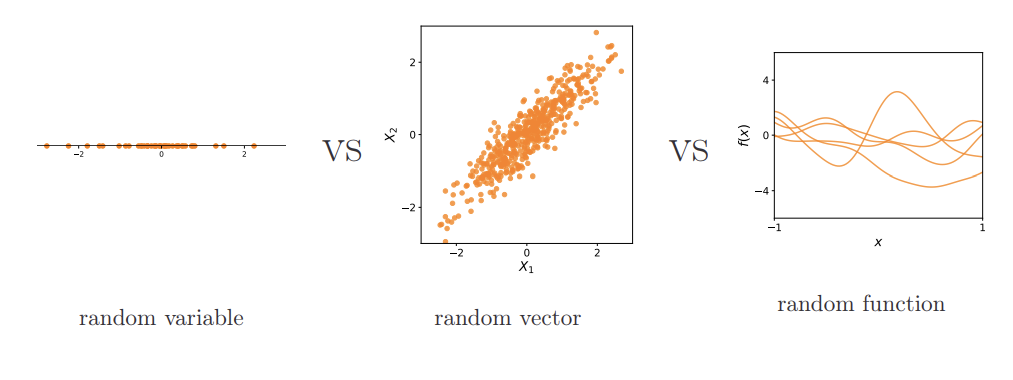
\includegraphics[scale=0.9]{Screenshot 2023-11-28 151344.png}
%     \caption{ \textcolor{red}{Screenshot noch nachbauen} Examples of a random variable, random vector and random process}
%     \label{fig:Screenshot 2023-11-28 151344.png}
% \end{figure}
% 
\begin{figure}[b]
    \centering
    %% Creator: Matplotlib, PGF backend
%%
%% To include the figure in your LaTeX document, write
%%   \input{<filename>.pgf}
%%
%% Make sure the required packages are loaded in your preamble
%%   \usepackage{pgf}
%%
%% Also ensure that all the required font packages are loaded; for instance,
%% the lmodern package is sometimes necessary when using math font.
%%   \usepackage{lmodern}
%%
%% Figures using additional raster images can only be included by \input if
%% they are in the same directory as the main LaTeX file. For loading figures
%% from other directories you can use the `import` package
%%   \usepackage{import}
%%
%% and then include the figures with
%%   \import{<path to file>}{<filename>.pgf}
%%
%% Matplotlib used the following preamble
%%   \def\mathdefault#1{#1}
%%   \everymath=\expandafter{\the\everymath\displaystyle}
%%   \usepackage[T1]{fontenc}
%%   \usepackage{siunitx}
%%   \usepackage{amssymb}
%%   \usepackage{amsmath}
%%   \makeatletter\@ifpackageloaded{underscore}{}{\usepackage[strings]{underscore}}\makeatother
%%
\begingroup%
\makeatletter%
\begin{pgfpicture}%
\pgfpathrectangle{\pgfpointorigin}{\pgfqpoint{5.788510in}{1.788748in}}%
\pgfusepath{use as bounding box, clip}%
\begin{pgfscope}%
\pgfsetbuttcap%
\pgfsetmiterjoin%
\definecolor{currentfill}{rgb}{1.000000,1.000000,1.000000}%
\pgfsetfillcolor{currentfill}%
\pgfsetlinewidth{0.000000pt}%
\definecolor{currentstroke}{rgb}{1.000000,1.000000,1.000000}%
\pgfsetstrokecolor{currentstroke}%
\pgfsetdash{}{0pt}%
\pgfpathmoveto{\pgfqpoint{0.000000in}{0.000000in}}%
\pgfpathlineto{\pgfqpoint{5.788510in}{0.000000in}}%
\pgfpathlineto{\pgfqpoint{5.788510in}{1.788748in}}%
\pgfpathlineto{\pgfqpoint{0.000000in}{1.788748in}}%
\pgfpathlineto{\pgfqpoint{0.000000in}{0.000000in}}%
\pgfpathclose%
\pgfusepath{fill}%
\end{pgfscope}%
\begin{pgfscope}%
\pgfsetbuttcap%
\pgfsetmiterjoin%
\definecolor{currentfill}{rgb}{1.000000,1.000000,1.000000}%
\pgfsetfillcolor{currentfill}%
\pgfsetlinewidth{0.000000pt}%
\definecolor{currentstroke}{rgb}{0.000000,0.000000,0.000000}%
\pgfsetstrokecolor{currentstroke}%
\pgfsetstrokeopacity{0.000000}%
\pgfsetdash{}{0pt}%
\pgfpathmoveto{\pgfqpoint{0.270378in}{0.150000in}}%
\pgfpathlineto{\pgfqpoint{1.759126in}{0.150000in}}%
\pgfpathlineto{\pgfqpoint{1.759126in}{1.638748in}}%
\pgfpathlineto{\pgfqpoint{0.270378in}{1.638748in}}%
\pgfpathlineto{\pgfqpoint{0.270378in}{0.150000in}}%
\pgfpathclose%
\pgfusepath{fill}%
\end{pgfscope}%
\begin{pgfscope}%
\pgfpathrectangle{\pgfqpoint{0.270378in}{0.150000in}}{\pgfqpoint{1.488748in}{1.488748in}}%
\pgfusepath{clip}%
\pgfsetbuttcap%
\pgfsetroundjoin%
\definecolor{currentfill}{rgb}{1.000000,0.745098,0.043137}%
\pgfsetfillcolor{currentfill}%
\pgfsetlinewidth{1.003750pt}%
\definecolor{currentstroke}{rgb}{1.000000,0.745098,0.043137}%
\pgfsetstrokecolor{currentstroke}%
\pgfsetdash{}{0pt}%
\pgfsys@defobject{currentmarker}{\pgfqpoint{-0.004910in}{-0.004910in}}{\pgfqpoint{0.004910in}{0.004910in}}{%
\pgfpathmoveto{\pgfqpoint{0.000000in}{-0.004910in}}%
\pgfpathcurveto{\pgfqpoint{0.001302in}{-0.004910in}}{\pgfqpoint{0.002551in}{-0.004393in}}{\pgfqpoint{0.003472in}{-0.003472in}}%
\pgfpathcurveto{\pgfqpoint{0.004393in}{-0.002551in}}{\pgfqpoint{0.004910in}{-0.001302in}}{\pgfqpoint{0.004910in}{0.000000in}}%
\pgfpathcurveto{\pgfqpoint{0.004910in}{0.001302in}}{\pgfqpoint{0.004393in}{0.002551in}}{\pgfqpoint{0.003472in}{0.003472in}}%
\pgfpathcurveto{\pgfqpoint{0.002551in}{0.004393in}}{\pgfqpoint{0.001302in}{0.004910in}}{\pgfqpoint{0.000000in}{0.004910in}}%
\pgfpathcurveto{\pgfqpoint{-0.001302in}{0.004910in}}{\pgfqpoint{-0.002551in}{0.004393in}}{\pgfqpoint{-0.003472in}{0.003472in}}%
\pgfpathcurveto{\pgfqpoint{-0.004393in}{0.002551in}}{\pgfqpoint{-0.004910in}{0.001302in}}{\pgfqpoint{-0.004910in}{0.000000in}}%
\pgfpathcurveto{\pgfqpoint{-0.004910in}{-0.001302in}}{\pgfqpoint{-0.004393in}{-0.002551in}}{\pgfqpoint{-0.003472in}{-0.003472in}}%
\pgfpathcurveto{\pgfqpoint{-0.002551in}{-0.004393in}}{\pgfqpoint{-0.001302in}{-0.004910in}}{\pgfqpoint{0.000000in}{-0.004910in}}%
\pgfpathlineto{\pgfqpoint{0.000000in}{-0.004910in}}%
\pgfpathclose%
\pgfusepath{stroke,fill}%
}%
\begin{pgfscope}%
\pgfsys@transformshift{0.853307in}{0.894374in}%
\pgfsys@useobject{currentmarker}{}%
\end{pgfscope}%
\begin{pgfscope}%
\pgfsys@transformshift{1.167420in}{0.894374in}%
\pgfsys@useobject{currentmarker}{}%
\end{pgfscope}%
\begin{pgfscope}%
\pgfsys@transformshift{0.912341in}{0.894374in}%
\pgfsys@useobject{currentmarker}{}%
\end{pgfscope}%
\begin{pgfscope}%
\pgfsys@transformshift{0.672276in}{0.894374in}%
\pgfsys@useobject{currentmarker}{}%
\end{pgfscope}%
\begin{pgfscope}%
\pgfsys@transformshift{1.272485in}{0.894374in}%
\pgfsys@useobject{currentmarker}{}%
\end{pgfscope}%
\begin{pgfscope}%
\pgfsys@transformshift{1.312703in}{0.894374in}%
\pgfsys@useobject{currentmarker}{}%
\end{pgfscope}%
\begin{pgfscope}%
\pgfsys@transformshift{1.120275in}{0.894374in}%
\pgfsys@useobject{currentmarker}{}%
\end{pgfscope}%
\begin{pgfscope}%
\pgfsys@transformshift{1.243541in}{0.894374in}%
\pgfsys@useobject{currentmarker}{}%
\end{pgfscope}%
\begin{pgfscope}%
\pgfsys@transformshift{1.163994in}{0.894374in}%
\pgfsys@useobject{currentmarker}{}%
\end{pgfscope}%
\begin{pgfscope}%
\pgfsys@transformshift{1.082993in}{0.894374in}%
\pgfsys@useobject{currentmarker}{}%
\end{pgfscope}%
\begin{pgfscope}%
\pgfsys@transformshift{0.999854in}{0.894374in}%
\pgfsys@useobject{currentmarker}{}%
\end{pgfscope}%
\begin{pgfscope}%
\pgfsys@transformshift{1.262962in}{0.894374in}%
\pgfsys@useobject{currentmarker}{}%
\end{pgfscope}%
\begin{pgfscope}%
\pgfsys@transformshift{1.115710in}{0.894374in}%
\pgfsys@useobject{currentmarker}{}%
\end{pgfscope}%
\begin{pgfscope}%
\pgfsys@transformshift{0.939936in}{0.894374in}%
\pgfsys@useobject{currentmarker}{}%
\end{pgfscope}%
\begin{pgfscope}%
\pgfsys@transformshift{1.264286in}{0.894374in}%
\pgfsys@useobject{currentmarker}{}%
\end{pgfscope}%
\begin{pgfscope}%
\pgfsys@transformshift{1.554554in}{0.894374in}%
\pgfsys@useobject{currentmarker}{}%
\end{pgfscope}%
\begin{pgfscope}%
\pgfsys@transformshift{0.959149in}{0.894374in}%
\pgfsys@useobject{currentmarker}{}%
\end{pgfscope}%
\begin{pgfscope}%
\pgfsys@transformshift{0.511618in}{0.894374in}%
\pgfsys@useobject{currentmarker}{}%
\end{pgfscope}%
\begin{pgfscope}%
\pgfsys@transformshift{0.864650in}{0.894374in}%
\pgfsys@useobject{currentmarker}{}%
\end{pgfscope}%
\begin{pgfscope}%
\pgfsys@transformshift{1.132848in}{0.894374in}%
\pgfsys@useobject{currentmarker}{}%
\end{pgfscope}%
\begin{pgfscope}%
\pgfsys@transformshift{0.719482in}{0.894374in}%
\pgfsys@useobject{currentmarker}{}%
\end{pgfscope}%
\begin{pgfscope}%
\pgfsys@transformshift{1.504550in}{0.894374in}%
\pgfsys@useobject{currentmarker}{}%
\end{pgfscope}%
\begin{pgfscope}%
\pgfsys@transformshift{1.065799in}{0.894374in}%
\pgfsys@useobject{currentmarker}{}%
\end{pgfscope}%
\begin{pgfscope}%
\pgfsys@transformshift{1.362636in}{0.894374in}%
\pgfsys@useobject{currentmarker}{}%
\end{pgfscope}%
\begin{pgfscope}%
\pgfsys@transformshift{0.973301in}{0.894374in}%
\pgfsys@useobject{currentmarker}{}%
\end{pgfscope}%
\begin{pgfscope}%
\pgfsys@transformshift{0.909890in}{0.894374in}%
\pgfsys@useobject{currentmarker}{}%
\end{pgfscope}%
\begin{pgfscope}%
\pgfsys@transformshift{0.963385in}{0.894374in}%
\pgfsys@useobject{currentmarker}{}%
\end{pgfscope}%
\begin{pgfscope}%
\pgfsys@transformshift{1.330969in}{0.894374in}%
\pgfsys@useobject{currentmarker}{}%
\end{pgfscope}%
\begin{pgfscope}%
\pgfsys@transformshift{1.041150in}{0.894374in}%
\pgfsys@useobject{currentmarker}{}%
\end{pgfscope}%
\begin{pgfscope}%
\pgfsys@transformshift{1.153722in}{0.894374in}%
\pgfsys@useobject{currentmarker}{}%
\end{pgfscope}%
\begin{pgfscope}%
\pgfsys@transformshift{0.992481in}{0.894374in}%
\pgfsys@useobject{currentmarker}{}%
\end{pgfscope}%
\begin{pgfscope}%
\pgfsys@transformshift{1.122912in}{0.894374in}%
\pgfsys@useobject{currentmarker}{}%
\end{pgfscope}%
\begin{pgfscope}%
\pgfsys@transformshift{0.338048in}{0.894374in}%
\pgfsys@useobject{currentmarker}{}%
\end{pgfscope}%
\begin{pgfscope}%
\pgfsys@transformshift{0.989402in}{0.894374in}%
\pgfsys@useobject{currentmarker}{}%
\end{pgfscope}%
\begin{pgfscope}%
\pgfsys@transformshift{0.642681in}{0.894374in}%
\pgfsys@useobject{currentmarker}{}%
\end{pgfscope}%
\begin{pgfscope}%
\pgfsys@transformshift{0.938698in}{0.894374in}%
\pgfsys@useobject{currentmarker}{}%
\end{pgfscope}%
\begin{pgfscope}%
\pgfsys@transformshift{1.648253in}{0.894374in}%
\pgfsys@useobject{currentmarker}{}%
\end{pgfscope}%
\begin{pgfscope}%
\pgfsys@transformshift{0.931664in}{0.894374in}%
\pgfsys@useobject{currentmarker}{}%
\end{pgfscope}%
\begin{pgfscope}%
\pgfsys@transformshift{1.105766in}{0.894374in}%
\pgfsys@useobject{currentmarker}{}%
\end{pgfscope}%
\begin{pgfscope}%
\pgfsys@transformshift{1.691455in}{0.894374in}%
\pgfsys@useobject{currentmarker}{}%
\end{pgfscope}%
\begin{pgfscope}%
\pgfsys@transformshift{1.490737in}{0.894374in}%
\pgfsys@useobject{currentmarker}{}%
\end{pgfscope}%
\begin{pgfscope}%
\pgfsys@transformshift{0.574491in}{0.894374in}%
\pgfsys@useobject{currentmarker}{}%
\end{pgfscope}%
\begin{pgfscope}%
\pgfsys@transformshift{1.437226in}{0.894374in}%
\pgfsys@useobject{currentmarker}{}%
\end{pgfscope}%
\begin{pgfscope}%
\pgfsys@transformshift{1.115643in}{0.894374in}%
\pgfsys@useobject{currentmarker}{}%
\end{pgfscope}%
\begin{pgfscope}%
\pgfsys@transformshift{1.047076in}{0.894374in}%
\pgfsys@useobject{currentmarker}{}%
\end{pgfscope}%
\begin{pgfscope}%
\pgfsys@transformshift{1.263964in}{0.894374in}%
\pgfsys@useobject{currentmarker}{}%
\end{pgfscope}%
\begin{pgfscope}%
\pgfsys@transformshift{1.019037in}{0.894374in}%
\pgfsys@useobject{currentmarker}{}%
\end{pgfscope}%
\begin{pgfscope}%
\pgfsys@transformshift{1.204106in}{0.894374in}%
\pgfsys@useobject{currentmarker}{}%
\end{pgfscope}%
\begin{pgfscope}%
\pgfsys@transformshift{1.103160in}{0.894374in}%
\pgfsys@useobject{currentmarker}{}%
\end{pgfscope}%
\begin{pgfscope}%
\pgfsys@transformshift{1.316196in}{0.894374in}%
\pgfsys@useobject{currentmarker}{}%
\end{pgfscope}%
\end{pgfscope}%
\begin{pgfscope}%
\pgfsetbuttcap%
\pgfsetmiterjoin%
\definecolor{currentfill}{rgb}{1.000000,1.000000,1.000000}%
\pgfsetfillcolor{currentfill}%
\pgfsetlinewidth{0.000000pt}%
\definecolor{currentstroke}{rgb}{0.000000,0.000000,0.000000}%
\pgfsetstrokecolor{currentstroke}%
\pgfsetstrokeopacity{0.000000}%
\pgfsetdash{}{0pt}%
\pgfpathmoveto{\pgfqpoint{2.149881in}{0.150000in}}%
\pgfpathlineto{\pgfqpoint{3.638629in}{0.150000in}}%
\pgfpathlineto{\pgfqpoint{3.638629in}{1.638748in}}%
\pgfpathlineto{\pgfqpoint{2.149881in}{1.638748in}}%
\pgfpathlineto{\pgfqpoint{2.149881in}{0.150000in}}%
\pgfpathclose%
\pgfusepath{fill}%
\end{pgfscope}%
\begin{pgfscope}%
\pgfpathrectangle{\pgfqpoint{2.149881in}{0.150000in}}{\pgfqpoint{1.488748in}{1.488748in}}%
\pgfusepath{clip}%
\pgfsetbuttcap%
\pgfsetroundjoin%
\definecolor{currentfill}{rgb}{1.000000,0.745098,0.043137}%
\pgfsetfillcolor{currentfill}%
\pgfsetlinewidth{1.003750pt}%
\definecolor{currentstroke}{rgb}{1.000000,0.745098,0.043137}%
\pgfsetstrokecolor{currentstroke}%
\pgfsetdash{}{0pt}%
\pgfsys@defobject{currentmarker}{\pgfqpoint{-0.004910in}{-0.004910in}}{\pgfqpoint{0.004910in}{0.004910in}}{%
\pgfpathmoveto{\pgfqpoint{0.000000in}{-0.004910in}}%
\pgfpathcurveto{\pgfqpoint{0.001302in}{-0.004910in}}{\pgfqpoint{0.002551in}{-0.004393in}}{\pgfqpoint{0.003472in}{-0.003472in}}%
\pgfpathcurveto{\pgfqpoint{0.004393in}{-0.002551in}}{\pgfqpoint{0.004910in}{-0.001302in}}{\pgfqpoint{0.004910in}{0.000000in}}%
\pgfpathcurveto{\pgfqpoint{0.004910in}{0.001302in}}{\pgfqpoint{0.004393in}{0.002551in}}{\pgfqpoint{0.003472in}{0.003472in}}%
\pgfpathcurveto{\pgfqpoint{0.002551in}{0.004393in}}{\pgfqpoint{0.001302in}{0.004910in}}{\pgfqpoint{0.000000in}{0.004910in}}%
\pgfpathcurveto{\pgfqpoint{-0.001302in}{0.004910in}}{\pgfqpoint{-0.002551in}{0.004393in}}{\pgfqpoint{-0.003472in}{0.003472in}}%
\pgfpathcurveto{\pgfqpoint{-0.004393in}{0.002551in}}{\pgfqpoint{-0.004910in}{0.001302in}}{\pgfqpoint{-0.004910in}{0.000000in}}%
\pgfpathcurveto{\pgfqpoint{-0.004910in}{-0.001302in}}{\pgfqpoint{-0.004393in}{-0.002551in}}{\pgfqpoint{-0.003472in}{-0.003472in}}%
\pgfpathcurveto{\pgfqpoint{-0.002551in}{-0.004393in}}{\pgfqpoint{-0.001302in}{-0.004910in}}{\pgfqpoint{0.000000in}{-0.004910in}}%
\pgfpathlineto{\pgfqpoint{0.000000in}{-0.004910in}}%
\pgfpathclose%
\pgfusepath{stroke,fill}%
}%
\begin{pgfscope}%
\pgfsys@transformshift{3.292183in}{0.820815in}%
\pgfsys@useobject{currentmarker}{}%
\end{pgfscope}%
\begin{pgfscope}%
\pgfsys@transformshift{2.766297in}{1.074182in}%
\pgfsys@useobject{currentmarker}{}%
\end{pgfscope}%
\begin{pgfscope}%
\pgfsys@transformshift{3.016164in}{0.868433in}%
\pgfsys@useobject{currentmarker}{}%
\end{pgfscope}%
\begin{pgfscope}%
\pgfsys@transformshift{3.393389in}{0.674793in}%
\pgfsys@useobject{currentmarker}{}%
\end{pgfscope}%
\begin{pgfscope}%
\pgfsys@transformshift{2.599394in}{1.158929in}%
\pgfsys@useobject{currentmarker}{}%
\end{pgfscope}%
\begin{pgfscope}%
\pgfsys@transformshift{2.698329in}{1.191369in}%
\pgfsys@useobject{currentmarker}{}%
\end{pgfscope}%
\begin{pgfscope}%
\pgfsys@transformshift{3.101029in}{1.036154in}%
\pgfsys@useobject{currentmarker}{}%
\end{pgfscope}%
\begin{pgfscope}%
\pgfsys@transformshift{2.814634in}{1.135583in}%
\pgfsys@useobject{currentmarker}{}%
\end{pgfscope}%
\begin{pgfscope}%
\pgfsys@transformshift{2.970497in}{1.071419in}%
\pgfsys@useobject{currentmarker}{}%
\end{pgfscope}%
\begin{pgfscope}%
\pgfsys@transformshift{3.199209in}{1.006082in}%
\pgfsys@useobject{currentmarker}{}%
\end{pgfscope}%
\begin{pgfscope}%
\pgfsys@transformshift{2.902039in}{0.939021in}%
\pgfsys@useobject{currentmarker}{}%
\end{pgfscope}%
\begin{pgfscope}%
\pgfsys@transformshift{2.812665in}{1.151247in}%
\pgfsys@useobject{currentmarker}{}%
\end{pgfscope}%
\begin{pgfscope}%
\pgfsys@transformshift{3.170300in}{1.032472in}%
\pgfsys@useobject{currentmarker}{}%
\end{pgfscope}%
\begin{pgfscope}%
\pgfsys@transformshift{3.124205in}{0.890691in}%
\pgfsys@useobject{currentmarker}{}%
\end{pgfscope}%
\begin{pgfscope}%
\pgfsys@transformshift{2.844550in}{1.152315in}%
\pgfsys@useobject{currentmarker}{}%
\end{pgfscope}%
\begin{pgfscope}%
\pgfsys@transformshift{2.877353in}{1.386449in}%
\pgfsys@useobject{currentmarker}{}%
\end{pgfscope}%
\begin{pgfscope}%
\pgfsys@transformshift{3.237843in}{0.906188in}%
\pgfsys@useobject{currentmarker}{}%
\end{pgfscope}%
\begin{pgfscope}%
\pgfsys@transformshift{3.271953in}{0.545204in}%
\pgfsys@useobject{currentmarker}{}%
\end{pgfscope}%
\begin{pgfscope}%
\pgfsys@transformshift{3.130046in}{0.829964in}%
\pgfsys@useobject{currentmarker}{}%
\end{pgfscope}%
\begin{pgfscope}%
\pgfsys@transformshift{2.732968in}{1.046296in}%
\pgfsys@useobject{currentmarker}{}%
\end{pgfscope}%
\begin{pgfscope}%
\pgfsys@transformshift{3.292562in}{0.712870in}%
\pgfsys@useobject{currentmarker}{}%
\end{pgfscope}%
\begin{pgfscope}%
\pgfsys@transformshift{2.482950in}{1.346115in}%
\pgfsys@useobject{currentmarker}{}%
\end{pgfscope}%
\begin{pgfscope}%
\pgfsys@transformshift{2.826043in}{0.992214in}%
\pgfsys@useobject{currentmarker}{}%
\end{pgfscope}%
\begin{pgfscope}%
\pgfsys@transformshift{2.777339in}{1.231646in}%
\pgfsys@useobject{currentmarker}{}%
\end{pgfscope}%
\begin{pgfscope}%
\pgfsys@transformshift{3.118964in}{0.917603in}%
\pgfsys@useobject{currentmarker}{}%
\end{pgfscope}%
\begin{pgfscope}%
\pgfsys@transformshift{3.099844in}{0.866455in}%
\pgfsys@useobject{currentmarker}{}%
\end{pgfscope}%
\begin{pgfscope}%
\pgfsys@transformshift{2.886776in}{0.909605in}%
\pgfsys@useobject{currentmarker}{}%
\end{pgfscope}%
\begin{pgfscope}%
\pgfsys@transformshift{2.528690in}{1.206103in}%
\pgfsys@useobject{currentmarker}{}%
\end{pgfscope}%
\begin{pgfscope}%
\pgfsys@transformshift{2.921993in}{0.972331in}%
\pgfsys@useobject{currentmarker}{}%
\end{pgfscope}%
\begin{pgfscope}%
\pgfsys@transformshift{2.820265in}{1.063134in}%
\pgfsys@useobject{currentmarker}{}%
\end{pgfscope}%
\begin{pgfscope}%
\pgfsys@transformshift{2.819231in}{0.933074in}%
\pgfsys@useobject{currentmarker}{}%
\end{pgfscope}%
\begin{pgfscope}%
\pgfsys@transformshift{2.909380in}{1.038282in}%
\pgfsys@useobject{currentmarker}{}%
\end{pgfscope}%
\begin{pgfscope}%
\pgfsys@transformshift{3.343094in}{0.405201in}%
\pgfsys@useobject{currentmarker}{}%
\end{pgfscope}%
\begin{pgfscope}%
\pgfsys@transformshift{3.210079in}{0.930591in}%
\pgfsys@useobject{currentmarker}{}%
\end{pgfscope}%
\begin{pgfscope}%
\pgfsys@transformshift{3.290044in}{0.650921in}%
\pgfsys@useobject{currentmarker}{}%
\end{pgfscope}%
\begin{pgfscope}%
\pgfsys@transformshift{2.956844in}{0.889692in}%
\pgfsys@useobject{currentmarker}{}%
\end{pgfscope}%
\begin{pgfscope}%
\pgfsys@transformshift{2.623165in}{1.462028in}%
\pgfsys@useobject{currentmarker}{}%
\end{pgfscope}%
\begin{pgfscope}%
\pgfsys@transformshift{2.891824in}{0.884019in}%
\pgfsys@useobject{currentmarker}{}%
\end{pgfscope}%
\begin{pgfscope}%
\pgfsys@transformshift{3.030991in}{1.024452in}%
\pgfsys@useobject{currentmarker}{}%
\end{pgfscope}%
\begin{pgfscope}%
\pgfsys@transformshift{2.900213in}{1.496876in}%
\pgfsys@useobject{currentmarker}{}%
\end{pgfscope}%
\begin{pgfscope}%
\pgfsys@transformshift{2.636254in}{1.334974in}%
\pgfsys@useobject{currentmarker}{}%
\end{pgfscope}%
\begin{pgfscope}%
\pgfsys@transformshift{3.274368in}{0.595918in}%
\pgfsys@useobject{currentmarker}{}%
\end{pgfscope}%
\begin{pgfscope}%
\pgfsys@transformshift{2.716049in}{1.291811in}%
\pgfsys@useobject{currentmarker}{}%
\end{pgfscope}%
\begin{pgfscope}%
\pgfsys@transformshift{2.888498in}{1.032418in}%
\pgfsys@useobject{currentmarker}{}%
\end{pgfscope}%
\begin{pgfscope}%
\pgfsys@transformshift{2.963671in}{0.977112in}%
\pgfsys@useobject{currentmarker}{}%
\end{pgfscope}%
\begin{pgfscope}%
\pgfsys@transformshift{2.966203in}{1.152056in}%
\pgfsys@useobject{currentmarker}{}%
\end{pgfscope}%
\begin{pgfscope}%
\pgfsys@transformshift{3.020282in}{0.954495in}%
\pgfsys@useobject{currentmarker}{}%
\end{pgfscope}%
\begin{pgfscope}%
\pgfsys@transformshift{3.020831in}{1.103774in}%
\pgfsys@useobject{currentmarker}{}%
\end{pgfscope}%
\begin{pgfscope}%
\pgfsys@transformshift{2.752522in}{1.022349in}%
\pgfsys@useobject{currentmarker}{}%
\end{pgfscope}%
\begin{pgfscope}%
\pgfsys@transformshift{2.841155in}{1.194187in}%
\pgfsys@useobject{currentmarker}{}%
\end{pgfscope}%
\begin{pgfscope}%
\pgfsys@transformshift{3.136736in}{0.805025in}%
\pgfsys@useobject{currentmarker}{}%
\end{pgfscope}%
\begin{pgfscope}%
\pgfsys@transformshift{2.918830in}{1.384175in}%
\pgfsys@useobject{currentmarker}{}%
\end{pgfscope}%
\begin{pgfscope}%
\pgfsys@transformshift{3.158122in}{0.516969in}%
\pgfsys@useobject{currentmarker}{}%
\end{pgfscope}%
\begin{pgfscope}%
\pgfsys@transformshift{3.150810in}{0.476784in}%
\pgfsys@useobject{currentmarker}{}%
\end{pgfscope}%
\begin{pgfscope}%
\pgfsys@transformshift{2.918541in}{0.795489in}%
\pgfsys@useobject{currentmarker}{}%
\end{pgfscope}%
\begin{pgfscope}%
\pgfsys@transformshift{2.437682in}{1.336634in}%
\pgfsys@useobject{currentmarker}{}%
\end{pgfscope}%
\begin{pgfscope}%
\pgfsys@transformshift{3.003925in}{1.039181in}%
\pgfsys@useobject{currentmarker}{}%
\end{pgfscope}%
\begin{pgfscope}%
\pgfsys@transformshift{3.398152in}{0.758225in}%
\pgfsys@useobject{currentmarker}{}%
\end{pgfscope}%
\begin{pgfscope}%
\pgfsys@transformshift{3.485491in}{0.460491in}%
\pgfsys@useobject{currentmarker}{}%
\end{pgfscope}%
\begin{pgfscope}%
\pgfsys@transformshift{2.879639in}{1.169808in}%
\pgfsys@useobject{currentmarker}{}%
\end{pgfscope}%
\begin{pgfscope}%
\pgfsys@transformshift{2.978119in}{0.986668in}%
\pgfsys@useobject{currentmarker}{}%
\end{pgfscope}%
\begin{pgfscope}%
\pgfsys@transformshift{2.438617in}{1.496893in}%
\pgfsys@useobject{currentmarker}{}%
\end{pgfscope}%
\begin{pgfscope}%
\pgfsys@transformshift{3.001535in}{1.218313in}%
\pgfsys@useobject{currentmarker}{}%
\end{pgfscope}%
\begin{pgfscope}%
\pgfsys@transformshift{2.639058in}{1.084074in}%
\pgfsys@useobject{currentmarker}{}%
\end{pgfscope}%
\begin{pgfscope}%
\pgfsys@transformshift{2.979408in}{1.121190in}%
\pgfsys@useobject{currentmarker}{}%
\end{pgfscope}%
\begin{pgfscope}%
\pgfsys@transformshift{3.176590in}{0.751090in}%
\pgfsys@useobject{currentmarker}{}%
\end{pgfscope}%
\begin{pgfscope}%
\pgfsys@transformshift{2.981850in}{1.173095in}%
\pgfsys@useobject{currentmarker}{}%
\end{pgfscope}%
\begin{pgfscope}%
\pgfsys@transformshift{3.202145in}{0.867681in}%
\pgfsys@useobject{currentmarker}{}%
\end{pgfscope}%
\begin{pgfscope}%
\pgfsys@transformshift{2.946546in}{1.141761in}%
\pgfsys@useobject{currentmarker}{}%
\end{pgfscope}%
\begin{pgfscope}%
\pgfsys@transformshift{2.948710in}{1.212875in}%
\pgfsys@useobject{currentmarker}{}%
\end{pgfscope}%
\begin{pgfscope}%
\pgfsys@transformshift{3.050329in}{0.771247in}%
\pgfsys@useobject{currentmarker}{}%
\end{pgfscope}%
\begin{pgfscope}%
\pgfsys@transformshift{3.570959in}{0.591994in}%
\pgfsys@useobject{currentmarker}{}%
\end{pgfscope}%
\begin{pgfscope}%
\pgfsys@transformshift{3.237305in}{0.991549in}%
\pgfsys@useobject{currentmarker}{}%
\end{pgfscope}%
\begin{pgfscope}%
\pgfsys@transformshift{2.670376in}{0.961162in}%
\pgfsys@useobject{currentmarker}{}%
\end{pgfscope}%
\begin{pgfscope}%
\pgfsys@transformshift{3.008122in}{1.170816in}%
\pgfsys@useobject{currentmarker}{}%
\end{pgfscope}%
\begin{pgfscope}%
\pgfsys@transformshift{3.128020in}{0.883333in}%
\pgfsys@useobject{currentmarker}{}%
\end{pgfscope}%
\begin{pgfscope}%
\pgfsys@transformshift{3.296901in}{1.044916in}%
\pgfsys@useobject{currentmarker}{}%
\end{pgfscope}%
\begin{pgfscope}%
\pgfsys@transformshift{3.022358in}{1.041996in}%
\pgfsys@useobject{currentmarker}{}%
\end{pgfscope}%
\begin{pgfscope}%
\pgfsys@transformshift{2.642266in}{1.096272in}%
\pgfsys@useobject{currentmarker}{}%
\end{pgfscope}%
\begin{pgfscope}%
\pgfsys@transformshift{2.910023in}{0.842787in}%
\pgfsys@useobject{currentmarker}{}%
\end{pgfscope}%
\begin{pgfscope}%
\pgfsys@transformshift{2.830219in}{1.434204in}%
\pgfsys@useobject{currentmarker}{}%
\end{pgfscope}%
\begin{pgfscope}%
\pgfsys@transformshift{3.055853in}{1.015857in}%
\pgfsys@useobject{currentmarker}{}%
\end{pgfscope}%
\begin{pgfscope}%
\pgfsys@transformshift{3.300423in}{0.422005in}%
\pgfsys@useobject{currentmarker}{}%
\end{pgfscope}%
\begin{pgfscope}%
\pgfsys@transformshift{3.156292in}{0.701305in}%
\pgfsys@useobject{currentmarker}{}%
\end{pgfscope}%
\begin{pgfscope}%
\pgfsys@transformshift{3.120431in}{1.027413in}%
\pgfsys@useobject{currentmarker}{}%
\end{pgfscope}%
\begin{pgfscope}%
\pgfsys@transformshift{2.826281in}{0.897525in}%
\pgfsys@useobject{currentmarker}{}%
\end{pgfscope}%
\begin{pgfscope}%
\pgfsys@transformshift{3.069099in}{1.224011in}%
\pgfsys@useobject{currentmarker}{}%
\end{pgfscope}%
\begin{pgfscope}%
\pgfsys@transformshift{2.856950in}{0.916958in}%
\pgfsys@useobject{currentmarker}{}%
\end{pgfscope}%
\begin{pgfscope}%
\pgfsys@transformshift{3.005903in}{0.783774in}%
\pgfsys@useobject{currentmarker}{}%
\end{pgfscope}%
\begin{pgfscope}%
\pgfsys@transformshift{2.590458in}{1.236556in}%
\pgfsys@useobject{currentmarker}{}%
\end{pgfscope}%
\begin{pgfscope}%
\pgfsys@transformshift{3.025202in}{0.870818in}%
\pgfsys@useobject{currentmarker}{}%
\end{pgfscope}%
\begin{pgfscope}%
\pgfsys@transformshift{2.861535in}{1.399076in}%
\pgfsys@useobject{currentmarker}{}%
\end{pgfscope}%
\begin{pgfscope}%
\pgfsys@transformshift{2.865465in}{1.046632in}%
\pgfsys@useobject{currentmarker}{}%
\end{pgfscope}%
\begin{pgfscope}%
\pgfsys@transformshift{3.291175in}{0.886398in}%
\pgfsys@useobject{currentmarker}{}%
\end{pgfscope}%
\begin{pgfscope}%
\pgfsys@transformshift{2.924942in}{0.973597in}%
\pgfsys@useobject{currentmarker}{}%
\end{pgfscope}%
\begin{pgfscope}%
\pgfsys@transformshift{3.158338in}{0.919368in}%
\pgfsys@useobject{currentmarker}{}%
\end{pgfscope}%
\begin{pgfscope}%
\pgfsys@transformshift{2.943787in}{0.803155in}%
\pgfsys@useobject{currentmarker}{}%
\end{pgfscope}%
\begin{pgfscope}%
\pgfsys@transformshift{2.821640in}{0.883277in}%
\pgfsys@useobject{currentmarker}{}%
\end{pgfscope}%
\begin{pgfscope}%
\pgfsys@transformshift{3.156815in}{0.656475in}%
\pgfsys@useobject{currentmarker}{}%
\end{pgfscope}%
\begin{pgfscope}%
\pgfsys@transformshift{2.999820in}{0.789821in}%
\pgfsys@useobject{currentmarker}{}%
\end{pgfscope}%
\begin{pgfscope}%
\pgfsys@transformshift{3.173224in}{1.095105in}%
\pgfsys@useobject{currentmarker}{}%
\end{pgfscope}%
\begin{pgfscope}%
\pgfsys@transformshift{3.070342in}{0.938471in}%
\pgfsys@useobject{currentmarker}{}%
\end{pgfscope}%
\begin{pgfscope}%
\pgfsys@transformshift{3.104600in}{0.574130in}%
\pgfsys@useobject{currentmarker}{}%
\end{pgfscope}%
\begin{pgfscope}%
\pgfsys@transformshift{2.937220in}{1.157010in}%
\pgfsys@useobject{currentmarker}{}%
\end{pgfscope}%
\begin{pgfscope}%
\pgfsys@transformshift{2.873278in}{0.765679in}%
\pgfsys@useobject{currentmarker}{}%
\end{pgfscope}%
\begin{pgfscope}%
\pgfsys@transformshift{2.984608in}{1.088477in}%
\pgfsys@useobject{currentmarker}{}%
\end{pgfscope}%
\begin{pgfscope}%
\pgfsys@transformshift{3.121201in}{0.559318in}%
\pgfsys@useobject{currentmarker}{}%
\end{pgfscope}%
\begin{pgfscope}%
\pgfsys@transformshift{2.898886in}{1.539487in}%
\pgfsys@useobject{currentmarker}{}%
\end{pgfscope}%
\begin{pgfscope}%
\pgfsys@transformshift{3.557581in}{0.830091in}%
\pgfsys@useobject{currentmarker}{}%
\end{pgfscope}%
\begin{pgfscope}%
\pgfsys@transformshift{2.854913in}{1.141458in}%
\pgfsys@useobject{currentmarker}{}%
\end{pgfscope}%
\begin{pgfscope}%
\pgfsys@transformshift{2.641077in}{1.058083in}%
\pgfsys@useobject{currentmarker}{}%
\end{pgfscope}%
\begin{pgfscope}%
\pgfsys@transformshift{3.052658in}{0.849811in}%
\pgfsys@useobject{currentmarker}{}%
\end{pgfscope}%
\begin{pgfscope}%
\pgfsys@transformshift{2.712948in}{1.135818in}%
\pgfsys@useobject{currentmarker}{}%
\end{pgfscope}%
\begin{pgfscope}%
\pgfsys@transformshift{3.025048in}{0.957884in}%
\pgfsys@useobject{currentmarker}{}%
\end{pgfscope}%
\begin{pgfscope}%
\pgfsys@transformshift{3.232194in}{0.644656in}%
\pgfsys@useobject{currentmarker}{}%
\end{pgfscope}%
\begin{pgfscope}%
\pgfsys@transformshift{3.174711in}{0.854507in}%
\pgfsys@useobject{currentmarker}{}%
\end{pgfscope}%
\begin{pgfscope}%
\pgfsys@transformshift{2.863597in}{0.880833in}%
\pgfsys@useobject{currentmarker}{}%
\end{pgfscope}%
\begin{pgfscope}%
\pgfsys@transformshift{2.810612in}{1.031985in}%
\pgfsys@useobject{currentmarker}{}%
\end{pgfscope}%
\begin{pgfscope}%
\pgfsys@transformshift{2.920240in}{1.125349in}%
\pgfsys@useobject{currentmarker}{}%
\end{pgfscope}%
\begin{pgfscope}%
\pgfsys@transformshift{3.129141in}{0.999864in}%
\pgfsys@useobject{currentmarker}{}%
\end{pgfscope}%
\begin{pgfscope}%
\pgfsys@transformshift{3.094856in}{0.893336in}%
\pgfsys@useobject{currentmarker}{}%
\end{pgfscope}%
\begin{pgfscope}%
\pgfsys@transformshift{3.004932in}{1.138651in}%
\pgfsys@useobject{currentmarker}{}%
\end{pgfscope}%
\begin{pgfscope}%
\pgfsys@transformshift{3.244151in}{0.398879in}%
\pgfsys@useobject{currentmarker}{}%
\end{pgfscope}%
\begin{pgfscope}%
\pgfsys@transformshift{2.876036in}{1.001852in}%
\pgfsys@useobject{currentmarker}{}%
\end{pgfscope}%
\begin{pgfscope}%
\pgfsys@transformshift{2.912317in}{0.933664in}%
\pgfsys@useobject{currentmarker}{}%
\end{pgfscope}%
\begin{pgfscope}%
\pgfsys@transformshift{2.942975in}{0.989561in}%
\pgfsys@useobject{currentmarker}{}%
\end{pgfscope}%
\begin{pgfscope}%
\pgfsys@transformshift{2.920816in}{1.406732in}%
\pgfsys@useobject{currentmarker}{}%
\end{pgfscope}%
\begin{pgfscope}%
\pgfsys@transformshift{3.016320in}{0.980359in}%
\pgfsys@useobject{currentmarker}{}%
\end{pgfscope}%
\begin{pgfscope}%
\pgfsys@transformshift{2.689784in}{1.199247in}%
\pgfsys@useobject{currentmarker}{}%
\end{pgfscope}%
\begin{pgfscope}%
\pgfsys@transformshift{3.102604in}{0.959324in}%
\pgfsys@useobject{currentmarker}{}%
\end{pgfscope}%
\begin{pgfscope}%
\pgfsys@transformshift{3.093733in}{0.873362in}%
\pgfsys@useobject{currentmarker}{}%
\end{pgfscope}%
\begin{pgfscope}%
\pgfsys@transformshift{3.094146in}{0.940765in}%
\pgfsys@useobject{currentmarker}{}%
\end{pgfscope}%
\begin{pgfscope}%
\pgfsys@transformshift{2.918473in}{1.085305in}%
\pgfsys@useobject{currentmarker}{}%
\end{pgfscope}%
\begin{pgfscope}%
\pgfsys@transformshift{2.963545in}{1.000984in}%
\pgfsys@useobject{currentmarker}{}%
\end{pgfscope}%
\begin{pgfscope}%
\pgfsys@transformshift{3.202927in}{0.660807in}%
\pgfsys@useobject{currentmarker}{}%
\end{pgfscope}%
\begin{pgfscope}%
\pgfsys@transformshift{3.214552in}{0.782652in}%
\pgfsys@useobject{currentmarker}{}%
\end{pgfscope}%
\begin{pgfscope}%
\pgfsys@transformshift{2.852498in}{1.165537in}%
\pgfsys@useobject{currentmarker}{}%
\end{pgfscope}%
\begin{pgfscope}%
\pgfsys@transformshift{2.979304in}{0.978036in}%
\pgfsys@useobject{currentmarker}{}%
\end{pgfscope}%
\begin{pgfscope}%
\pgfsys@transformshift{3.075529in}{1.045012in}%
\pgfsys@useobject{currentmarker}{}%
\end{pgfscope}%
\begin{pgfscope}%
\pgfsys@transformshift{2.683744in}{1.260661in}%
\pgfsys@useobject{currentmarker}{}%
\end{pgfscope}%
\begin{pgfscope}%
\pgfsys@transformshift{2.914105in}{0.960025in}%
\pgfsys@useobject{currentmarker}{}%
\end{pgfscope}%
\begin{pgfscope}%
\pgfsys@transformshift{2.739068in}{1.388912in}%
\pgfsys@useobject{currentmarker}{}%
\end{pgfscope}%
\begin{pgfscope}%
\pgfsys@transformshift{2.829750in}{1.215005in}%
\pgfsys@useobject{currentmarker}{}%
\end{pgfscope}%
\begin{pgfscope}%
\pgfsys@transformshift{2.959678in}{0.909226in}%
\pgfsys@useobject{currentmarker}{}%
\end{pgfscope}%
\begin{pgfscope}%
\pgfsys@transformshift{3.449945in}{0.564964in}%
\pgfsys@useobject{currentmarker}{}%
\end{pgfscope}%
\begin{pgfscope}%
\pgfsys@transformshift{2.869755in}{0.996159in}%
\pgfsys@useobject{currentmarker}{}%
\end{pgfscope}%
\begin{pgfscope}%
\pgfsys@transformshift{3.121885in}{1.167109in}%
\pgfsys@useobject{currentmarker}{}%
\end{pgfscope}%
\begin{pgfscope}%
\pgfsys@transformshift{2.632255in}{1.262669in}%
\pgfsys@useobject{currentmarker}{}%
\end{pgfscope}%
\begin{pgfscope}%
\pgfsys@transformshift{3.096825in}{0.679577in}%
\pgfsys@useobject{currentmarker}{}%
\end{pgfscope}%
\begin{pgfscope}%
\pgfsys@transformshift{2.843016in}{1.285787in}%
\pgfsys@useobject{currentmarker}{}%
\end{pgfscope}%
\begin{pgfscope}%
\pgfsys@transformshift{3.123207in}{0.711252in}%
\pgfsys@useobject{currentmarker}{}%
\end{pgfscope}%
\begin{pgfscope}%
\pgfsys@transformshift{2.815359in}{1.458044in}%
\pgfsys@useobject{currentmarker}{}%
\end{pgfscope}%
\begin{pgfscope}%
\pgfsys@transformshift{3.316818in}{0.898133in}%
\pgfsys@useobject{currentmarker}{}%
\end{pgfscope}%
\begin{pgfscope}%
\pgfsys@transformshift{3.065039in}{0.812145in}%
\pgfsys@useobject{currentmarker}{}%
\end{pgfscope}%
\begin{pgfscope}%
\pgfsys@transformshift{2.791945in}{1.398995in}%
\pgfsys@useobject{currentmarker}{}%
\end{pgfscope}%
\begin{pgfscope}%
\pgfsys@transformshift{3.055654in}{1.030715in}%
\pgfsys@useobject{currentmarker}{}%
\end{pgfscope}%
\begin{pgfscope}%
\pgfsys@transformshift{2.661285in}{1.213917in}%
\pgfsys@useobject{currentmarker}{}%
\end{pgfscope}%
\begin{pgfscope}%
\pgfsys@transformshift{3.013580in}{0.845917in}%
\pgfsys@useobject{currentmarker}{}%
\end{pgfscope}%
\begin{pgfscope}%
\pgfsys@transformshift{2.699226in}{1.170671in}%
\pgfsys@useobject{currentmarker}{}%
\end{pgfscope}%
\begin{pgfscope}%
\pgfsys@transformshift{3.047210in}{0.945306in}%
\pgfsys@useobject{currentmarker}{}%
\end{pgfscope}%
\begin{pgfscope}%
\pgfsys@transformshift{2.626336in}{1.088588in}%
\pgfsys@useobject{currentmarker}{}%
\end{pgfscope}%
\begin{pgfscope}%
\pgfsys@transformshift{3.058079in}{0.664534in}%
\pgfsys@useobject{currentmarker}{}%
\end{pgfscope}%
\begin{pgfscope}%
\pgfsys@transformshift{3.024086in}{1.037259in}%
\pgfsys@useobject{currentmarker}{}%
\end{pgfscope}%
\begin{pgfscope}%
\pgfsys@transformshift{2.791240in}{1.215283in}%
\pgfsys@useobject{currentmarker}{}%
\end{pgfscope}%
\begin{pgfscope}%
\pgfsys@transformshift{2.953239in}{1.288366in}%
\pgfsys@useobject{currentmarker}{}%
\end{pgfscope}%
\begin{pgfscope}%
\pgfsys@transformshift{2.646429in}{0.942844in}%
\pgfsys@useobject{currentmarker}{}%
\end{pgfscope}%
\begin{pgfscope}%
\pgfsys@transformshift{2.983775in}{0.997191in}%
\pgfsys@useobject{currentmarker}{}%
\end{pgfscope}%
\begin{pgfscope}%
\pgfsys@transformshift{3.004487in}{0.894879in}%
\pgfsys@useobject{currentmarker}{}%
\end{pgfscope}%
\begin{pgfscope}%
\pgfsys@transformshift{3.281238in}{0.869980in}%
\pgfsys@useobject{currentmarker}{}%
\end{pgfscope}%
\begin{pgfscope}%
\pgfsys@transformshift{2.871144in}{1.324557in}%
\pgfsys@useobject{currentmarker}{}%
\end{pgfscope}%
\begin{pgfscope}%
\pgfsys@transformshift{2.982777in}{0.842417in}%
\pgfsys@useobject{currentmarker}{}%
\end{pgfscope}%
\begin{pgfscope}%
\pgfsys@transformshift{3.374172in}{0.565067in}%
\pgfsys@useobject{currentmarker}{}%
\end{pgfscope}%
\begin{pgfscope}%
\pgfsys@transformshift{3.051627in}{1.214210in}%
\pgfsys@useobject{currentmarker}{}%
\end{pgfscope}%
\begin{pgfscope}%
\pgfsys@transformshift{2.677908in}{1.374981in}%
\pgfsys@useobject{currentmarker}{}%
\end{pgfscope}%
\begin{pgfscope}%
\pgfsys@transformshift{3.187682in}{0.662551in}%
\pgfsys@useobject{currentmarker}{}%
\end{pgfscope}%
\begin{pgfscope}%
\pgfsys@transformshift{3.286411in}{0.774165in}%
\pgfsys@useobject{currentmarker}{}%
\end{pgfscope}%
\begin{pgfscope}%
\pgfsys@transformshift{2.862629in}{0.890600in}%
\pgfsys@useobject{currentmarker}{}%
\end{pgfscope}%
\begin{pgfscope}%
\pgfsys@transformshift{3.041578in}{0.947571in}%
\pgfsys@useobject{currentmarker}{}%
\end{pgfscope}%
\begin{pgfscope}%
\pgfsys@transformshift{2.401452in}{1.471491in}%
\pgfsys@useobject{currentmarker}{}%
\end{pgfscope}%
\begin{pgfscope}%
\pgfsys@transformshift{3.174531in}{1.298846in}%
\pgfsys@useobject{currentmarker}{}%
\end{pgfscope}%
\begin{pgfscope}%
\pgfsys@transformshift{2.844434in}{1.255549in}%
\pgfsys@useobject{currentmarker}{}%
\end{pgfscope}%
\begin{pgfscope}%
\pgfsys@transformshift{3.234125in}{0.887545in}%
\pgfsys@useobject{currentmarker}{}%
\end{pgfscope}%
\begin{pgfscope}%
\pgfsys@transformshift{2.647015in}{1.245579in}%
\pgfsys@useobject{currentmarker}{}%
\end{pgfscope}%
\begin{pgfscope}%
\pgfsys@transformshift{3.145613in}{0.681581in}%
\pgfsys@useobject{currentmarker}{}%
\end{pgfscope}%
\begin{pgfscope}%
\pgfsys@transformshift{2.586067in}{1.485707in}%
\pgfsys@useobject{currentmarker}{}%
\end{pgfscope}%
\begin{pgfscope}%
\pgfsys@transformshift{2.910840in}{0.861979in}%
\pgfsys@useobject{currentmarker}{}%
\end{pgfscope}%
\begin{pgfscope}%
\pgfsys@transformshift{3.406288in}{0.548875in}%
\pgfsys@useobject{currentmarker}{}%
\end{pgfscope}%
\begin{pgfscope}%
\pgfsys@transformshift{3.066617in}{0.885869in}%
\pgfsys@useobject{currentmarker}{}%
\end{pgfscope}%
\begin{pgfscope}%
\pgfsys@transformshift{2.824636in}{1.200267in}%
\pgfsys@useobject{currentmarker}{}%
\end{pgfscope}%
\begin{pgfscope}%
\pgfsys@transformshift{3.125578in}{0.607552in}%
\pgfsys@useobject{currentmarker}{}%
\end{pgfscope}%
\begin{pgfscope}%
\pgfsys@transformshift{2.920466in}{0.880506in}%
\pgfsys@useobject{currentmarker}{}%
\end{pgfscope}%
\begin{pgfscope}%
\pgfsys@transformshift{3.253620in}{0.614471in}%
\pgfsys@useobject{currentmarker}{}%
\end{pgfscope}%
\begin{pgfscope}%
\pgfsys@transformshift{2.790432in}{1.130466in}%
\pgfsys@useobject{currentmarker}{}%
\end{pgfscope}%
\begin{pgfscope}%
\pgfsys@transformshift{2.851006in}{1.018205in}%
\pgfsys@useobject{currentmarker}{}%
\end{pgfscope}%
\begin{pgfscope}%
\pgfsys@transformshift{2.890346in}{1.152986in}%
\pgfsys@useobject{currentmarker}{}%
\end{pgfscope}%
\begin{pgfscope}%
\pgfsys@transformshift{3.424638in}{0.651927in}%
\pgfsys@useobject{currentmarker}{}%
\end{pgfscope}%
\begin{pgfscope}%
\pgfsys@transformshift{2.920046in}{1.052695in}%
\pgfsys@useobject{currentmarker}{}%
\end{pgfscope}%
\begin{pgfscope}%
\pgfsys@transformshift{2.835011in}{1.322858in}%
\pgfsys@useobject{currentmarker}{}%
\end{pgfscope}%
\begin{pgfscope}%
\pgfsys@transformshift{2.936000in}{1.054641in}%
\pgfsys@useobject{currentmarker}{}%
\end{pgfscope}%
\begin{pgfscope}%
\pgfsys@transformshift{3.110445in}{0.801524in}%
\pgfsys@useobject{currentmarker}{}%
\end{pgfscope}%
\begin{pgfscope}%
\pgfsys@transformshift{3.066199in}{0.799135in}%
\pgfsys@useobject{currentmarker}{}%
\end{pgfscope}%
\begin{pgfscope}%
\pgfsys@transformshift{2.935950in}{1.092062in}%
\pgfsys@useobject{currentmarker}{}%
\end{pgfscope}%
\begin{pgfscope}%
\pgfsys@transformshift{3.016239in}{1.012304in}%
\pgfsys@useobject{currentmarker}{}%
\end{pgfscope}%
\begin{pgfscope}%
\pgfsys@transformshift{3.159909in}{0.507711in}%
\pgfsys@useobject{currentmarker}{}%
\end{pgfscope}%
\begin{pgfscope}%
\pgfsys@transformshift{3.226691in}{0.584194in}%
\pgfsys@useobject{currentmarker}{}%
\end{pgfscope}%
\begin{pgfscope}%
\pgfsys@transformshift{3.241230in}{0.897990in}%
\pgfsys@useobject{currentmarker}{}%
\end{pgfscope}%
\begin{pgfscope}%
\pgfsys@transformshift{3.285832in}{1.081665in}%
\pgfsys@useobject{currentmarker}{}%
\end{pgfscope}%
\begin{pgfscope}%
\pgfsys@transformshift{2.927381in}{1.571078in}%
\pgfsys@useobject{currentmarker}{}%
\end{pgfscope}%
\begin{pgfscope}%
\pgfsys@transformshift{2.898682in}{0.828718in}%
\pgfsys@useobject{currentmarker}{}%
\end{pgfscope}%
\begin{pgfscope}%
\pgfsys@transformshift{2.861293in}{1.316472in}%
\pgfsys@useobject{currentmarker}{}%
\end{pgfscope}%
\begin{pgfscope}%
\pgfsys@transformshift{3.134296in}{0.593433in}%
\pgfsys@useobject{currentmarker}{}%
\end{pgfscope}%
\begin{pgfscope}%
\pgfsys@transformshift{3.316794in}{0.895138in}%
\pgfsys@useobject{currentmarker}{}%
\end{pgfscope}%
\begin{pgfscope}%
\pgfsys@transformshift{3.201397in}{0.783526in}%
\pgfsys@useobject{currentmarker}{}%
\end{pgfscope}%
\begin{pgfscope}%
\pgfsys@transformshift{3.149550in}{1.010088in}%
\pgfsys@useobject{currentmarker}{}%
\end{pgfscope}%
\begin{pgfscope}%
\pgfsys@transformshift{3.071829in}{1.110799in}%
\pgfsys@useobject{currentmarker}{}%
\end{pgfscope}%
\begin{pgfscope}%
\pgfsys@transformshift{3.284958in}{0.814290in}%
\pgfsys@useobject{currentmarker}{}%
\end{pgfscope}%
\begin{pgfscope}%
\pgfsys@transformshift{2.747716in}{1.041350in}%
\pgfsys@useobject{currentmarker}{}%
\end{pgfscope}%
\begin{pgfscope}%
\pgfsys@transformshift{2.964135in}{0.904984in}%
\pgfsys@useobject{currentmarker}{}%
\end{pgfscope}%
\begin{pgfscope}%
\pgfsys@transformshift{3.025203in}{1.077550in}%
\pgfsys@useobject{currentmarker}{}%
\end{pgfscope}%
\begin{pgfscope}%
\pgfsys@transformshift{2.864995in}{0.855295in}%
\pgfsys@useobject{currentmarker}{}%
\end{pgfscope}%
\begin{pgfscope}%
\pgfsys@transformshift{3.265287in}{0.807112in}%
\pgfsys@useobject{currentmarker}{}%
\end{pgfscope}%
\begin{pgfscope}%
\pgfsys@transformshift{3.150380in}{0.687340in}%
\pgfsys@useobject{currentmarker}{}%
\end{pgfscope}%
\begin{pgfscope}%
\pgfsys@transformshift{2.803474in}{1.009844in}%
\pgfsys@useobject{currentmarker}{}%
\end{pgfscope}%
\begin{pgfscope}%
\pgfsys@transformshift{2.752925in}{1.235995in}%
\pgfsys@useobject{currentmarker}{}%
\end{pgfscope}%
\begin{pgfscope}%
\pgfsys@transformshift{2.977014in}{0.821904in}%
\pgfsys@useobject{currentmarker}{}%
\end{pgfscope}%
\begin{pgfscope}%
\pgfsys@transformshift{2.816606in}{1.221421in}%
\pgfsys@useobject{currentmarker}{}%
\end{pgfscope}%
\begin{pgfscope}%
\pgfsys@transformshift{2.894225in}{0.895540in}%
\pgfsys@useobject{currentmarker}{}%
\end{pgfscope}%
\begin{pgfscope}%
\pgfsys@transformshift{2.997422in}{0.823691in}%
\pgfsys@useobject{currentmarker}{}%
\end{pgfscope}%
\begin{pgfscope}%
\pgfsys@transformshift{2.995687in}{0.694161in}%
\pgfsys@useobject{currentmarker}{}%
\end{pgfscope}%
\begin{pgfscope}%
\pgfsys@transformshift{3.289196in}{0.865126in}%
\pgfsys@useobject{currentmarker}{}%
\end{pgfscope}%
\begin{pgfscope}%
\pgfsys@transformshift{3.059483in}{0.639801in}%
\pgfsys@useobject{currentmarker}{}%
\end{pgfscope}%
\begin{pgfscope}%
\pgfsys@transformshift{3.028542in}{0.682118in}%
\pgfsys@useobject{currentmarker}{}%
\end{pgfscope}%
\begin{pgfscope}%
\pgfsys@transformshift{3.226091in}{0.731902in}%
\pgfsys@useobject{currentmarker}{}%
\end{pgfscope}%
\begin{pgfscope}%
\pgfsys@transformshift{3.101773in}{1.043266in}%
\pgfsys@useobject{currentmarker}{}%
\end{pgfscope}%
\begin{pgfscope}%
\pgfsys@transformshift{2.890276in}{0.999136in}%
\pgfsys@useobject{currentmarker}{}%
\end{pgfscope}%
\begin{pgfscope}%
\pgfsys@transformshift{3.131723in}{0.789695in}%
\pgfsys@useobject{currentmarker}{}%
\end{pgfscope}%
\begin{pgfscope}%
\pgfsys@transformshift{2.838713in}{0.747415in}%
\pgfsys@useobject{currentmarker}{}%
\end{pgfscope}%
\begin{pgfscope}%
\pgfsys@transformshift{2.928147in}{1.359986in}%
\pgfsys@useobject{currentmarker}{}%
\end{pgfscope}%
\begin{pgfscope}%
\pgfsys@transformshift{3.179841in}{0.852648in}%
\pgfsys@useobject{currentmarker}{}%
\end{pgfscope}%
\begin{pgfscope}%
\pgfsys@transformshift{3.187444in}{0.555453in}%
\pgfsys@useobject{currentmarker}{}%
\end{pgfscope}%
\begin{pgfscope}%
\pgfsys@transformshift{2.873007in}{1.205906in}%
\pgfsys@useobject{currentmarker}{}%
\end{pgfscope}%
\begin{pgfscope}%
\pgfsys@transformshift{3.145863in}{0.919401in}%
\pgfsys@useobject{currentmarker}{}%
\end{pgfscope}%
\begin{pgfscope}%
\pgfsys@transformshift{3.084058in}{1.018329in}%
\pgfsys@useobject{currentmarker}{}%
\end{pgfscope}%
\begin{pgfscope}%
\pgfsys@transformshift{2.791788in}{1.182681in}%
\pgfsys@useobject{currentmarker}{}%
\end{pgfscope}%
\begin{pgfscope}%
\pgfsys@transformshift{2.981500in}{0.811015in}%
\pgfsys@useobject{currentmarker}{}%
\end{pgfscope}%
\begin{pgfscope}%
\pgfsys@transformshift{2.994330in}{0.711549in}%
\pgfsys@useobject{currentmarker}{}%
\end{pgfscope}%
\begin{pgfscope}%
\pgfsys@transformshift{2.990715in}{1.054127in}%
\pgfsys@useobject{currentmarker}{}%
\end{pgfscope}%
\begin{pgfscope}%
\pgfsys@transformshift{2.995212in}{1.104053in}%
\pgfsys@useobject{currentmarker}{}%
\end{pgfscope}%
\begin{pgfscope}%
\pgfsys@transformshift{3.056392in}{0.825860in}%
\pgfsys@useobject{currentmarker}{}%
\end{pgfscope}%
\begin{pgfscope}%
\pgfsys@transformshift{3.327238in}{0.535627in}%
\pgfsys@useobject{currentmarker}{}%
\end{pgfscope}%
\begin{pgfscope}%
\pgfsys@transformshift{3.169416in}{1.079834in}%
\pgfsys@useobject{currentmarker}{}%
\end{pgfscope}%
\begin{pgfscope}%
\pgfsys@transformshift{3.072677in}{0.592282in}%
\pgfsys@useobject{currentmarker}{}%
\end{pgfscope}%
\begin{pgfscope}%
\pgfsys@transformshift{2.905835in}{0.975576in}%
\pgfsys@useobject{currentmarker}{}%
\end{pgfscope}%
\begin{pgfscope}%
\pgfsys@transformshift{2.870101in}{1.081041in}%
\pgfsys@useobject{currentmarker}{}%
\end{pgfscope}%
\begin{pgfscope}%
\pgfsys@transformshift{3.021668in}{0.887747in}%
\pgfsys@useobject{currentmarker}{}%
\end{pgfscope}%
\begin{pgfscope}%
\pgfsys@transformshift{2.826586in}{1.245456in}%
\pgfsys@useobject{currentmarker}{}%
\end{pgfscope}%
\begin{pgfscope}%
\pgfsys@transformshift{3.002716in}{1.107618in}%
\pgfsys@useobject{currentmarker}{}%
\end{pgfscope}%
\begin{pgfscope}%
\pgfsys@transformshift{3.173648in}{1.007282in}%
\pgfsys@useobject{currentmarker}{}%
\end{pgfscope}%
\begin{pgfscope}%
\pgfsys@transformshift{3.146638in}{0.962588in}%
\pgfsys@useobject{currentmarker}{}%
\end{pgfscope}%
\begin{pgfscope}%
\pgfsys@transformshift{2.883048in}{1.008050in}%
\pgfsys@useobject{currentmarker}{}%
\end{pgfscope}%
\begin{pgfscope}%
\pgfsys@transformshift{2.994848in}{0.740435in}%
\pgfsys@useobject{currentmarker}{}%
\end{pgfscope}%
\begin{pgfscope}%
\pgfsys@transformshift{2.217551in}{1.553487in}%
\pgfsys@useobject{currentmarker}{}%
\end{pgfscope}%
\begin{pgfscope}%
\pgfsys@transformshift{3.108308in}{0.894403in}%
\pgfsys@useobject{currentmarker}{}%
\end{pgfscope}%
\begin{pgfscope}%
\pgfsys@transformshift{2.749041in}{1.327893in}%
\pgfsys@useobject{currentmarker}{}%
\end{pgfscope}%
\begin{pgfscope}%
\pgfsys@transformshift{3.153716in}{0.898932in}%
\pgfsys@useobject{currentmarker}{}%
\end{pgfscope}%
\begin{pgfscope}%
\pgfsys@transformshift{3.072293in}{0.823237in}%
\pgfsys@useobject{currentmarker}{}%
\end{pgfscope}%
\begin{pgfscope}%
\pgfsys@transformshift{3.035683in}{0.962697in}%
\pgfsys@useobject{currentmarker}{}%
\end{pgfscope}%
\begin{pgfscope}%
\pgfsys@transformshift{2.854733in}{0.985463in}%
\pgfsys@useobject{currentmarker}{}%
\end{pgfscope}%
\begin{pgfscope}%
\pgfsys@transformshift{2.806779in}{1.083455in}%
\pgfsys@useobject{currentmarker}{}%
\end{pgfscope}%
\begin{pgfscope}%
\pgfsys@transformshift{2.981379in}{1.064423in}%
\pgfsys@useobject{currentmarker}{}%
\end{pgfscope}%
\begin{pgfscope}%
\pgfsys@transformshift{2.949546in}{1.289246in}%
\pgfsys@useobject{currentmarker}{}%
\end{pgfscope}%
\begin{pgfscope}%
\pgfsys@transformshift{2.812983in}{1.293145in}%
\pgfsys@useobject{currentmarker}{}%
\end{pgfscope}%
\begin{pgfscope}%
\pgfsys@transformshift{2.645336in}{1.309468in}%
\pgfsys@useobject{currentmarker}{}%
\end{pgfscope}%
\begin{pgfscope}%
\pgfsys@transformshift{2.918687in}{0.826539in}%
\pgfsys@useobject{currentmarker}{}%
\end{pgfscope}%
\begin{pgfscope}%
\pgfsys@transformshift{3.023696in}{1.071983in}%
\pgfsys@useobject{currentmarker}{}%
\end{pgfscope}%
\begin{pgfscope}%
\pgfsys@transformshift{3.007341in}{1.052387in}%
\pgfsys@useobject{currentmarker}{}%
\end{pgfscope}%
\begin{pgfscope}%
\pgfsys@transformshift{3.080234in}{0.942307in}%
\pgfsys@useobject{currentmarker}{}%
\end{pgfscope}%
\begin{pgfscope}%
\pgfsys@transformshift{2.672484in}{1.311777in}%
\pgfsys@useobject{currentmarker}{}%
\end{pgfscope}%
\begin{pgfscope}%
\pgfsys@transformshift{2.886710in}{0.844550in}%
\pgfsys@useobject{currentmarker}{}%
\end{pgfscope}%
\begin{pgfscope}%
\pgfsys@transformshift{2.957145in}{1.142165in}%
\pgfsys@useobject{currentmarker}{}%
\end{pgfscope}%
\begin{pgfscope}%
\pgfsys@transformshift{2.616521in}{1.491444in}%
\pgfsys@useobject{currentmarker}{}%
\end{pgfscope}%
\begin{pgfscope}%
\pgfsys@transformshift{3.227527in}{0.777477in}%
\pgfsys@useobject{currentmarker}{}%
\end{pgfscope}%
\begin{pgfscope}%
\pgfsys@transformshift{3.058283in}{0.641502in}%
\pgfsys@useobject{currentmarker}{}%
\end{pgfscope}%
\begin{pgfscope}%
\pgfsys@transformshift{2.543075in}{1.240150in}%
\pgfsys@useobject{currentmarker}{}%
\end{pgfscope}%
\begin{pgfscope}%
\pgfsys@transformshift{2.841202in}{1.104570in}%
\pgfsys@useobject{currentmarker}{}%
\end{pgfscope}%
\begin{pgfscope}%
\pgfsys@transformshift{2.903883in}{1.131914in}%
\pgfsys@useobject{currentmarker}{}%
\end{pgfscope}%
\begin{pgfscope}%
\pgfsys@transformshift{3.016160in}{0.913461in}%
\pgfsys@useobject{currentmarker}{}%
\end{pgfscope}%
\begin{pgfscope}%
\pgfsys@transformshift{3.343819in}{0.613925in}%
\pgfsys@useobject{currentmarker}{}%
\end{pgfscope}%
\begin{pgfscope}%
\pgfsys@transformshift{3.083851in}{0.910327in}%
\pgfsys@useobject{currentmarker}{}%
\end{pgfscope}%
\begin{pgfscope}%
\pgfsys@transformshift{3.082833in}{0.577260in}%
\pgfsys@useobject{currentmarker}{}%
\end{pgfscope}%
\begin{pgfscope}%
\pgfsys@transformshift{2.655315in}{0.803902in}%
\pgfsys@useobject{currentmarker}{}%
\end{pgfscope}%
\begin{pgfscope}%
\pgfsys@transformshift{3.132428in}{1.006310in}%
\pgfsys@useobject{currentmarker}{}%
\end{pgfscope}%
\begin{pgfscope}%
\pgfsys@transformshift{3.062688in}{0.978316in}%
\pgfsys@useobject{currentmarker}{}%
\end{pgfscope}%
\begin{pgfscope}%
\pgfsys@transformshift{2.685977in}{1.179315in}%
\pgfsys@useobject{currentmarker}{}%
\end{pgfscope}%
\begin{pgfscope}%
\pgfsys@transformshift{3.071020in}{0.795836in}%
\pgfsys@useobject{currentmarker}{}%
\end{pgfscope}%
\begin{pgfscope}%
\pgfsys@transformshift{2.542290in}{1.246744in}%
\pgfsys@useobject{currentmarker}{}%
\end{pgfscope}%
\begin{pgfscope}%
\pgfsys@transformshift{3.086898in}{0.896116in}%
\pgfsys@useobject{currentmarker}{}%
\end{pgfscope}%
\begin{pgfscope}%
\pgfsys@transformshift{2.958453in}{0.713218in}%
\pgfsys@useobject{currentmarker}{}%
\end{pgfscope}%
\begin{pgfscope}%
\pgfsys@transformshift{3.035796in}{1.034195in}%
\pgfsys@useobject{currentmarker}{}%
\end{pgfscope}%
\begin{pgfscope}%
\pgfsys@transformshift{2.801996in}{1.353089in}%
\pgfsys@useobject{currentmarker}{}%
\end{pgfscope}%
\begin{pgfscope}%
\pgfsys@transformshift{3.066195in}{0.970207in}%
\pgfsys@useobject{currentmarker}{}%
\end{pgfscope}%
\begin{pgfscope}%
\pgfsys@transformshift{3.104442in}{0.977244in}%
\pgfsys@useobject{currentmarker}{}%
\end{pgfscope}%
\begin{pgfscope}%
\pgfsys@transformshift{2.992001in}{0.746750in}%
\pgfsys@useobject{currentmarker}{}%
\end{pgfscope}%
\begin{pgfscope}%
\pgfsys@transformshift{3.282048in}{0.632577in}%
\pgfsys@useobject{currentmarker}{}%
\end{pgfscope}%
\begin{pgfscope}%
\pgfsys@transformshift{3.142806in}{0.666625in}%
\pgfsys@useobject{currentmarker}{}%
\end{pgfscope}%
\begin{pgfscope}%
\pgfsys@transformshift{3.016842in}{0.955939in}%
\pgfsys@useobject{currentmarker}{}%
\end{pgfscope}%
\begin{pgfscope}%
\pgfsys@transformshift{2.999787in}{0.780473in}%
\pgfsys@useobject{currentmarker}{}%
\end{pgfscope}%
\begin{pgfscope}%
\pgfsys@transformshift{2.827643in}{1.207635in}%
\pgfsys@useobject{currentmarker}{}%
\end{pgfscope}%
\begin{pgfscope}%
\pgfsys@transformshift{2.860997in}{1.050616in}%
\pgfsys@useobject{currentmarker}{}%
\end{pgfscope}%
\begin{pgfscope}%
\pgfsys@transformshift{2.761176in}{0.897790in}%
\pgfsys@useobject{currentmarker}{}%
\end{pgfscope}%
\begin{pgfscope}%
\pgfsys@transformshift{2.947267in}{1.132670in}%
\pgfsys@useobject{currentmarker}{}%
\end{pgfscope}%
\begin{pgfscope}%
\pgfsys@transformshift{3.092659in}{0.789606in}%
\pgfsys@useobject{currentmarker}{}%
\end{pgfscope}%
\begin{pgfscope}%
\pgfsys@transformshift{2.795421in}{1.217776in}%
\pgfsys@useobject{currentmarker}{}%
\end{pgfscope}%
\begin{pgfscope}%
\pgfsys@transformshift{3.047749in}{1.091251in}%
\pgfsys@useobject{currentmarker}{}%
\end{pgfscope}%
\begin{pgfscope}%
\pgfsys@transformshift{2.977999in}{0.939470in}%
\pgfsys@useobject{currentmarker}{}%
\end{pgfscope}%
\begin{pgfscope}%
\pgfsys@transformshift{2.644358in}{1.029719in}%
\pgfsys@useobject{currentmarker}{}%
\end{pgfscope}%
\begin{pgfscope}%
\pgfsys@transformshift{2.745091in}{1.221213in}%
\pgfsys@useobject{currentmarker}{}%
\end{pgfscope}%
\begin{pgfscope}%
\pgfsys@transformshift{2.984113in}{1.081003in}%
\pgfsys@useobject{currentmarker}{}%
\end{pgfscope}%
\begin{pgfscope}%
\pgfsys@transformshift{2.850224in}{1.116181in}%
\pgfsys@useobject{currentmarker}{}%
\end{pgfscope}%
\begin{pgfscope}%
\pgfsys@transformshift{2.909297in}{0.721070in}%
\pgfsys@useobject{currentmarker}{}%
\end{pgfscope}%
\begin{pgfscope}%
\pgfsys@transformshift{2.995849in}{0.843292in}%
\pgfsys@useobject{currentmarker}{}%
\end{pgfscope}%
\begin{pgfscope}%
\pgfsys@transformshift{2.732299in}{0.781870in}%
\pgfsys@useobject{currentmarker}{}%
\end{pgfscope}%
\begin{pgfscope}%
\pgfsys@transformshift{3.321596in}{0.649965in}%
\pgfsys@useobject{currentmarker}{}%
\end{pgfscope}%
\begin{pgfscope}%
\pgfsys@transformshift{2.824073in}{1.085251in}%
\pgfsys@useobject{currentmarker}{}%
\end{pgfscope}%
\begin{pgfscope}%
\pgfsys@transformshift{2.744616in}{1.252831in}%
\pgfsys@useobject{currentmarker}{}%
\end{pgfscope}%
\begin{pgfscope}%
\pgfsys@transformshift{2.895649in}{1.020958in}%
\pgfsys@useobject{currentmarker}{}%
\end{pgfscope}%
\begin{pgfscope}%
\pgfsys@transformshift{2.918302in}{1.001851in}%
\pgfsys@useobject{currentmarker}{}%
\end{pgfscope}%
\begin{pgfscope}%
\pgfsys@transformshift{3.161082in}{0.836590in}%
\pgfsys@useobject{currentmarker}{}%
\end{pgfscope}%
\begin{pgfscope}%
\pgfsys@transformshift{2.996654in}{1.016167in}%
\pgfsys@useobject{currentmarker}{}%
\end{pgfscope}%
\begin{pgfscope}%
\pgfsys@transformshift{2.993770in}{1.208911in}%
\pgfsys@useobject{currentmarker}{}%
\end{pgfscope}%
\begin{pgfscope}%
\pgfsys@transformshift{2.929759in}{1.089328in}%
\pgfsys@useobject{currentmarker}{}%
\end{pgfscope}%
\begin{pgfscope}%
\pgfsys@transformshift{2.562340in}{1.304422in}%
\pgfsys@useobject{currentmarker}{}%
\end{pgfscope}%
\begin{pgfscope}%
\pgfsys@transformshift{3.099749in}{0.753191in}%
\pgfsys@useobject{currentmarker}{}%
\end{pgfscope}%
\begin{pgfscope}%
\pgfsys@transformshift{3.096681in}{0.878377in}%
\pgfsys@useobject{currentmarker}{}%
\end{pgfscope}%
\begin{pgfscope}%
\pgfsys@transformshift{3.105511in}{1.026248in}%
\pgfsys@useobject{currentmarker}{}%
\end{pgfscope}%
\begin{pgfscope}%
\pgfsys@transformshift{2.882855in}{0.894067in}%
\pgfsys@useobject{currentmarker}{}%
\end{pgfscope}%
\begin{pgfscope}%
\pgfsys@transformshift{2.472879in}{1.377108in}%
\pgfsys@useobject{currentmarker}{}%
\end{pgfscope}%
\begin{pgfscope}%
\pgfsys@transformshift{2.824972in}{0.858208in}%
\pgfsys@useobject{currentmarker}{}%
\end{pgfscope}%
\begin{pgfscope}%
\pgfsys@transformshift{3.226503in}{0.698909in}%
\pgfsys@useobject{currentmarker}{}%
\end{pgfscope}%
\begin{pgfscope}%
\pgfsys@transformshift{2.986144in}{0.899518in}%
\pgfsys@useobject{currentmarker}{}%
\end{pgfscope}%
\begin{pgfscope}%
\pgfsys@transformshift{2.518057in}{1.301075in}%
\pgfsys@useobject{currentmarker}{}%
\end{pgfscope}%
\begin{pgfscope}%
\pgfsys@transformshift{2.539626in}{1.489981in}%
\pgfsys@useobject{currentmarker}{}%
\end{pgfscope}%
\begin{pgfscope}%
\pgfsys@transformshift{3.103134in}{1.096328in}%
\pgfsys@useobject{currentmarker}{}%
\end{pgfscope}%
\begin{pgfscope}%
\pgfsys@transformshift{2.817967in}{0.998702in}%
\pgfsys@useobject{currentmarker}{}%
\end{pgfscope}%
\begin{pgfscope}%
\pgfsys@transformshift{2.919349in}{1.178097in}%
\pgfsys@useobject{currentmarker}{}%
\end{pgfscope}%
\begin{pgfscope}%
\pgfsys@transformshift{2.852554in}{1.030327in}%
\pgfsys@useobject{currentmarker}{}%
\end{pgfscope}%
\begin{pgfscope}%
\pgfsys@transformshift{3.066724in}{0.744688in}%
\pgfsys@useobject{currentmarker}{}%
\end{pgfscope}%
\begin{pgfscope}%
\pgfsys@transformshift{2.667791in}{0.966561in}%
\pgfsys@useobject{currentmarker}{}%
\end{pgfscope}%
\begin{pgfscope}%
\pgfsys@transformshift{3.250267in}{0.682811in}%
\pgfsys@useobject{currentmarker}{}%
\end{pgfscope}%
\begin{pgfscope}%
\pgfsys@transformshift{3.181745in}{0.638187in}%
\pgfsys@useobject{currentmarker}{}%
\end{pgfscope}%
\begin{pgfscope}%
\pgfsys@transformshift{2.851867in}{0.998988in}%
\pgfsys@useobject{currentmarker}{}%
\end{pgfscope}%
\begin{pgfscope}%
\pgfsys@transformshift{3.053936in}{0.890392in}%
\pgfsys@useobject{currentmarker}{}%
\end{pgfscope}%
\begin{pgfscope}%
\pgfsys@transformshift{3.318362in}{0.441902in}%
\pgfsys@useobject{currentmarker}{}%
\end{pgfscope}%
\begin{pgfscope}%
\pgfsys@transformshift{3.098725in}{0.888289in}%
\pgfsys@useobject{currentmarker}{}%
\end{pgfscope}%
\begin{pgfscope}%
\pgfsys@transformshift{3.006676in}{0.996168in}%
\pgfsys@useobject{currentmarker}{}%
\end{pgfscope}%
\begin{pgfscope}%
\pgfsys@transformshift{2.913369in}{1.412573in}%
\pgfsys@useobject{currentmarker}{}%
\end{pgfscope}%
\begin{pgfscope}%
\pgfsys@transformshift{2.991034in}{1.289735in}%
\pgfsys@useobject{currentmarker}{}%
\end{pgfscope}%
\begin{pgfscope}%
\pgfsys@transformshift{3.036112in}{0.932132in}%
\pgfsys@useobject{currentmarker}{}%
\end{pgfscope}%
\begin{pgfscope}%
\pgfsys@transformshift{2.912964in}{1.137673in}%
\pgfsys@useobject{currentmarker}{}%
\end{pgfscope}%
\begin{pgfscope}%
\pgfsys@transformshift{3.048930in}{0.563847in}%
\pgfsys@useobject{currentmarker}{}%
\end{pgfscope}%
\begin{pgfscope}%
\pgfsys@transformshift{3.212797in}{0.881194in}%
\pgfsys@useobject{currentmarker}{}%
\end{pgfscope}%
\begin{pgfscope}%
\pgfsys@transformshift{3.273589in}{0.855321in}%
\pgfsys@useobject{currentmarker}{}%
\end{pgfscope}%
\begin{pgfscope}%
\pgfsys@transformshift{3.158506in}{0.693081in}%
\pgfsys@useobject{currentmarker}{}%
\end{pgfscope}%
\begin{pgfscope}%
\pgfsys@transformshift{3.033112in}{0.662631in}%
\pgfsys@useobject{currentmarker}{}%
\end{pgfscope}%
\begin{pgfscope}%
\pgfsys@transformshift{2.796056in}{1.306802in}%
\pgfsys@useobject{currentmarker}{}%
\end{pgfscope}%
\begin{pgfscope}%
\pgfsys@transformshift{2.924436in}{1.046861in}%
\pgfsys@useobject{currentmarker}{}%
\end{pgfscope}%
\begin{pgfscope}%
\pgfsys@transformshift{2.734863in}{1.457864in}%
\pgfsys@useobject{currentmarker}{}%
\end{pgfscope}%
\begin{pgfscope}%
\pgfsys@transformshift{3.033122in}{0.862255in}%
\pgfsys@useobject{currentmarker}{}%
\end{pgfscope}%
\begin{pgfscope}%
\pgfsys@transformshift{3.003565in}{1.060725in}%
\pgfsys@useobject{currentmarker}{}%
\end{pgfscope}%
\begin{pgfscope}%
\pgfsys@transformshift{2.820578in}{0.974261in}%
\pgfsys@useobject{currentmarker}{}%
\end{pgfscope}%
\begin{pgfscope}%
\pgfsys@transformshift{3.084468in}{0.828148in}%
\pgfsys@useobject{currentmarker}{}%
\end{pgfscope}%
\begin{pgfscope}%
\pgfsys@transformshift{3.182684in}{0.746078in}%
\pgfsys@useobject{currentmarker}{}%
\end{pgfscope}%
\begin{pgfscope}%
\pgfsys@transformshift{3.240088in}{0.693023in}%
\pgfsys@useobject{currentmarker}{}%
\end{pgfscope}%
\begin{pgfscope}%
\pgfsys@transformshift{2.850981in}{1.060437in}%
\pgfsys@useobject{currentmarker}{}%
\end{pgfscope}%
\begin{pgfscope}%
\pgfsys@transformshift{3.280528in}{0.678340in}%
\pgfsys@useobject{currentmarker}{}%
\end{pgfscope}%
\begin{pgfscope}%
\pgfsys@transformshift{2.981862in}{1.057842in}%
\pgfsys@useobject{currentmarker}{}%
\end{pgfscope}%
\begin{pgfscope}%
\pgfsys@transformshift{2.742181in}{1.019781in}%
\pgfsys@useobject{currentmarker}{}%
\end{pgfscope}%
\begin{pgfscope}%
\pgfsys@transformshift{2.946344in}{0.932454in}%
\pgfsys@useobject{currentmarker}{}%
\end{pgfscope}%
\begin{pgfscope}%
\pgfsys@transformshift{3.052191in}{1.028290in}%
\pgfsys@useobject{currentmarker}{}%
\end{pgfscope}%
\begin{pgfscope}%
\pgfsys@transformshift{2.494778in}{1.140348in}%
\pgfsys@useobject{currentmarker}{}%
\end{pgfscope}%
\begin{pgfscope}%
\pgfsys@transformshift{3.181412in}{0.912873in}%
\pgfsys@useobject{currentmarker}{}%
\end{pgfscope}%
\begin{pgfscope}%
\pgfsys@transformshift{2.956618in}{0.791702in}%
\pgfsys@useobject{currentmarker}{}%
\end{pgfscope}%
\begin{pgfscope}%
\pgfsys@transformshift{3.208178in}{0.720425in}%
\pgfsys@useobject{currentmarker}{}%
\end{pgfscope}%
\begin{pgfscope}%
\pgfsys@transformshift{3.075102in}{0.992545in}%
\pgfsys@useobject{currentmarker}{}%
\end{pgfscope}%
\begin{pgfscope}%
\pgfsys@transformshift{2.800419in}{1.066397in}%
\pgfsys@useobject{currentmarker}{}%
\end{pgfscope}%
\begin{pgfscope}%
\pgfsys@transformshift{2.563504in}{1.109795in}%
\pgfsys@useobject{currentmarker}{}%
\end{pgfscope}%
\begin{pgfscope}%
\pgfsys@transformshift{3.191964in}{1.197572in}%
\pgfsys@useobject{currentmarker}{}%
\end{pgfscope}%
\begin{pgfscope}%
\pgfsys@transformshift{2.667559in}{1.038451in}%
\pgfsys@useobject{currentmarker}{}%
\end{pgfscope}%
\begin{pgfscope}%
\pgfsys@transformshift{2.990930in}{1.042998in}%
\pgfsys@useobject{currentmarker}{}%
\end{pgfscope}%
\begin{pgfscope}%
\pgfsys@transformshift{2.800030in}{1.224102in}%
\pgfsys@useobject{currentmarker}{}%
\end{pgfscope}%
\begin{pgfscope}%
\pgfsys@transformshift{2.725123in}{1.240310in}%
\pgfsys@useobject{currentmarker}{}%
\end{pgfscope}%
\begin{pgfscope}%
\pgfsys@transformshift{2.811034in}{0.613667in}%
\pgfsys@useobject{currentmarker}{}%
\end{pgfscope}%
\begin{pgfscope}%
\pgfsys@transformshift{2.903101in}{1.206994in}%
\pgfsys@useobject{currentmarker}{}%
\end{pgfscope}%
\begin{pgfscope}%
\pgfsys@transformshift{2.585311in}{1.328221in}%
\pgfsys@useobject{currentmarker}{}%
\end{pgfscope}%
\begin{pgfscope}%
\pgfsys@transformshift{3.190923in}{0.747423in}%
\pgfsys@useobject{currentmarker}{}%
\end{pgfscope}%
\begin{pgfscope}%
\pgfsys@transformshift{2.837396in}{0.784598in}%
\pgfsys@useobject{currentmarker}{}%
\end{pgfscope}%
\begin{pgfscope}%
\pgfsys@transformshift{2.729540in}{1.227670in}%
\pgfsys@useobject{currentmarker}{}%
\end{pgfscope}%
\begin{pgfscope}%
\pgfsys@transformshift{2.763314in}{1.206741in}%
\pgfsys@useobject{currentmarker}{}%
\end{pgfscope}%
\begin{pgfscope}%
\pgfsys@transformshift{2.928682in}{1.025285in}%
\pgfsys@useobject{currentmarker}{}%
\end{pgfscope}%
\begin{pgfscope}%
\pgfsys@transformshift{2.958841in}{1.145920in}%
\pgfsys@useobject{currentmarker}{}%
\end{pgfscope}%
\begin{pgfscope}%
\pgfsys@transformshift{2.784837in}{1.150247in}%
\pgfsys@useobject{currentmarker}{}%
\end{pgfscope}%
\begin{pgfscope}%
\pgfsys@transformshift{3.225188in}{0.958202in}%
\pgfsys@useobject{currentmarker}{}%
\end{pgfscope}%
\begin{pgfscope}%
\pgfsys@transformshift{2.527150in}{1.374640in}%
\pgfsys@useobject{currentmarker}{}%
\end{pgfscope}%
\begin{pgfscope}%
\pgfsys@transformshift{3.076410in}{0.756060in}%
\pgfsys@useobject{currentmarker}{}%
\end{pgfscope}%
\begin{pgfscope}%
\pgfsys@transformshift{2.548272in}{1.096129in}%
\pgfsys@useobject{currentmarker}{}%
\end{pgfscope}%
\begin{pgfscope}%
\pgfsys@transformshift{2.856904in}{1.090838in}%
\pgfsys@useobject{currentmarker}{}%
\end{pgfscope}%
\begin{pgfscope}%
\pgfsys@transformshift{3.290171in}{0.716302in}%
\pgfsys@useobject{currentmarker}{}%
\end{pgfscope}%
\begin{pgfscope}%
\pgfsys@transformshift{3.081425in}{0.936804in}%
\pgfsys@useobject{currentmarker}{}%
\end{pgfscope}%
\begin{pgfscope}%
\pgfsys@transformshift{2.952818in}{1.224766in}%
\pgfsys@useobject{currentmarker}{}%
\end{pgfscope}%
\begin{pgfscope}%
\pgfsys@transformshift{2.996790in}{1.200327in}%
\pgfsys@useobject{currentmarker}{}%
\end{pgfscope}%
\begin{pgfscope}%
\pgfsys@transformshift{2.819071in}{1.350880in}%
\pgfsys@useobject{currentmarker}{}%
\end{pgfscope}%
\begin{pgfscope}%
\pgfsys@transformshift{2.945537in}{0.959595in}%
\pgfsys@useobject{currentmarker}{}%
\end{pgfscope}%
\begin{pgfscope}%
\pgfsys@transformshift{3.230045in}{0.592126in}%
\pgfsys@useobject{currentmarker}{}%
\end{pgfscope}%
\begin{pgfscope}%
\pgfsys@transformshift{3.012956in}{0.628213in}%
\pgfsys@useobject{currentmarker}{}%
\end{pgfscope}%
\begin{pgfscope}%
\pgfsys@transformshift{2.862770in}{1.179942in}%
\pgfsys@useobject{currentmarker}{}%
\end{pgfscope}%
\begin{pgfscope}%
\pgfsys@transformshift{3.148709in}{0.809398in}%
\pgfsys@useobject{currentmarker}{}%
\end{pgfscope}%
\begin{pgfscope}%
\pgfsys@transformshift{2.776830in}{1.276250in}%
\pgfsys@useobject{currentmarker}{}%
\end{pgfscope}%
\begin{pgfscope}%
\pgfsys@transformshift{3.099141in}{1.427570in}%
\pgfsys@useobject{currentmarker}{}%
\end{pgfscope}%
\begin{pgfscope}%
\pgfsys@transformshift{2.696227in}{1.101778in}%
\pgfsys@useobject{currentmarker}{}%
\end{pgfscope}%
\begin{pgfscope}%
\pgfsys@transformshift{3.009393in}{1.114117in}%
\pgfsys@useobject{currentmarker}{}%
\end{pgfscope}%
\begin{pgfscope}%
\pgfsys@transformshift{2.978766in}{0.861477in}%
\pgfsys@useobject{currentmarker}{}%
\end{pgfscope}%
\begin{pgfscope}%
\pgfsys@transformshift{2.810570in}{1.021682in}%
\pgfsys@useobject{currentmarker}{}%
\end{pgfscope}%
\begin{pgfscope}%
\pgfsys@transformshift{2.807648in}{1.310504in}%
\pgfsys@useobject{currentmarker}{}%
\end{pgfscope}%
\begin{pgfscope}%
\pgfsys@transformshift{2.565055in}{1.259425in}%
\pgfsys@useobject{currentmarker}{}%
\end{pgfscope}%
\begin{pgfscope}%
\pgfsys@transformshift{3.330608in}{0.710430in}%
\pgfsys@useobject{currentmarker}{}%
\end{pgfscope}%
\begin{pgfscope}%
\pgfsys@transformshift{3.141884in}{1.084774in}%
\pgfsys@useobject{currentmarker}{}%
\end{pgfscope}%
\begin{pgfscope}%
\pgfsys@transformshift{2.995713in}{0.953591in}%
\pgfsys@useobject{currentmarker}{}%
\end{pgfscope}%
\begin{pgfscope}%
\pgfsys@transformshift{3.247116in}{0.781278in}%
\pgfsys@useobject{currentmarker}{}%
\end{pgfscope}%
\begin{pgfscope}%
\pgfsys@transformshift{3.278341in}{0.580608in}%
\pgfsys@useobject{currentmarker}{}%
\end{pgfscope}%
\begin{pgfscope}%
\pgfsys@transformshift{2.844465in}{0.982626in}%
\pgfsys@useobject{currentmarker}{}%
\end{pgfscope}%
\begin{pgfscope}%
\pgfsys@transformshift{2.590869in}{1.541412in}%
\pgfsys@useobject{currentmarker}{}%
\end{pgfscope}%
\begin{pgfscope}%
\pgfsys@transformshift{2.755554in}{1.241917in}%
\pgfsys@useobject{currentmarker}{}%
\end{pgfscope}%
\begin{pgfscope}%
\pgfsys@transformshift{2.964505in}{0.855184in}%
\pgfsys@useobject{currentmarker}{}%
\end{pgfscope}%
\begin{pgfscope}%
\pgfsys@transformshift{2.675204in}{1.413633in}%
\pgfsys@useobject{currentmarker}{}%
\end{pgfscope}%
\begin{pgfscope}%
\pgfsys@transformshift{3.098941in}{0.908696in}%
\pgfsys@useobject{currentmarker}{}%
\end{pgfscope}%
\begin{pgfscope}%
\pgfsys@transformshift{2.959089in}{1.220062in}%
\pgfsys@useobject{currentmarker}{}%
\end{pgfscope}%
\begin{pgfscope}%
\pgfsys@transformshift{2.596569in}{1.312605in}%
\pgfsys@useobject{currentmarker}{}%
\end{pgfscope}%
\begin{pgfscope}%
\pgfsys@transformshift{2.991840in}{1.071949in}%
\pgfsys@useobject{currentmarker}{}%
\end{pgfscope}%
\begin{pgfscope}%
\pgfsys@transformshift{3.194473in}{0.630528in}%
\pgfsys@useobject{currentmarker}{}%
\end{pgfscope}%
\begin{pgfscope}%
\pgfsys@transformshift{3.118920in}{1.146310in}%
\pgfsys@useobject{currentmarker}{}%
\end{pgfscope}%
\begin{pgfscope}%
\pgfsys@transformshift{2.963145in}{1.117625in}%
\pgfsys@useobject{currentmarker}{}%
\end{pgfscope}%
\begin{pgfscope}%
\pgfsys@transformshift{3.074792in}{0.996672in}%
\pgfsys@useobject{currentmarker}{}%
\end{pgfscope}%
\begin{pgfscope}%
\pgfsys@transformshift{2.991234in}{0.744919in}%
\pgfsys@useobject{currentmarker}{}%
\end{pgfscope}%
\begin{pgfscope}%
\pgfsys@transformshift{2.889122in}{1.285187in}%
\pgfsys@useobject{currentmarker}{}%
\end{pgfscope}%
\begin{pgfscope}%
\pgfsys@transformshift{3.083790in}{0.830614in}%
\pgfsys@useobject{currentmarker}{}%
\end{pgfscope}%
\begin{pgfscope}%
\pgfsys@transformshift{2.425850in}{1.128301in}%
\pgfsys@useobject{currentmarker}{}%
\end{pgfscope}%
\begin{pgfscope}%
\pgfsys@transformshift{2.836986in}{0.998856in}%
\pgfsys@useobject{currentmarker}{}%
\end{pgfscope}%
\begin{pgfscope}%
\pgfsys@transformshift{3.123406in}{0.534412in}%
\pgfsys@useobject{currentmarker}{}%
\end{pgfscope}%
\begin{pgfscope}%
\pgfsys@transformshift{2.845111in}{0.891730in}%
\pgfsys@useobject{currentmarker}{}%
\end{pgfscope}%
\begin{pgfscope}%
\pgfsys@transformshift{3.314048in}{0.759197in}%
\pgfsys@useobject{currentmarker}{}%
\end{pgfscope}%
\begin{pgfscope}%
\pgfsys@transformshift{2.959722in}{0.744742in}%
\pgfsys@useobject{currentmarker}{}%
\end{pgfscope}%
\begin{pgfscope}%
\pgfsys@transformshift{3.378219in}{0.663583in}%
\pgfsys@useobject{currentmarker}{}%
\end{pgfscope}%
\begin{pgfscope}%
\pgfsys@transformshift{2.986217in}{1.138297in}%
\pgfsys@useobject{currentmarker}{}%
\end{pgfscope}%
\begin{pgfscope}%
\pgfsys@transformshift{3.118729in}{0.821711in}%
\pgfsys@useobject{currentmarker}{}%
\end{pgfscope}%
\begin{pgfscope}%
\pgfsys@transformshift{2.952154in}{0.801766in}%
\pgfsys@useobject{currentmarker}{}%
\end{pgfscope}%
\begin{pgfscope}%
\pgfsys@transformshift{3.122456in}{0.765578in}%
\pgfsys@useobject{currentmarker}{}%
\end{pgfscope}%
\begin{pgfscope}%
\pgfsys@transformshift{3.082341in}{1.088473in}%
\pgfsys@useobject{currentmarker}{}%
\end{pgfscope}%
\begin{pgfscope}%
\pgfsys@transformshift{3.025422in}{1.201698in}%
\pgfsys@useobject{currentmarker}{}%
\end{pgfscope}%
\begin{pgfscope}%
\pgfsys@transformshift{3.112862in}{1.253617in}%
\pgfsys@useobject{currentmarker}{}%
\end{pgfscope}%
\begin{pgfscope}%
\pgfsys@transformshift{3.128250in}{1.122591in}%
\pgfsys@useobject{currentmarker}{}%
\end{pgfscope}%
\begin{pgfscope}%
\pgfsys@transformshift{3.313246in}{0.820016in}%
\pgfsys@useobject{currentmarker}{}%
\end{pgfscope}%
\begin{pgfscope}%
\pgfsys@transformshift{3.020789in}{0.923511in}%
\pgfsys@useobject{currentmarker}{}%
\end{pgfscope}%
\begin{pgfscope}%
\pgfsys@transformshift{2.998140in}{1.072149in}%
\pgfsys@useobject{currentmarker}{}%
\end{pgfscope}%
\begin{pgfscope}%
\pgfsys@transformshift{3.228482in}{0.793779in}%
\pgfsys@useobject{currentmarker}{}%
\end{pgfscope}%
\begin{pgfscope}%
\pgfsys@transformshift{2.909910in}{1.148539in}%
\pgfsys@useobject{currentmarker}{}%
\end{pgfscope}%
\begin{pgfscope}%
\pgfsys@transformshift{2.730618in}{0.968269in}%
\pgfsys@useobject{currentmarker}{}%
\end{pgfscope}%
\begin{pgfscope}%
\pgfsys@transformshift{2.883045in}{1.145029in}%
\pgfsys@useobject{currentmarker}{}%
\end{pgfscope}%
\begin{pgfscope}%
\pgfsys@transformshift{3.255951in}{0.715011in}%
\pgfsys@useobject{currentmarker}{}%
\end{pgfscope}%
\begin{pgfscope}%
\pgfsys@transformshift{3.138490in}{0.923373in}%
\pgfsys@useobject{currentmarker}{}%
\end{pgfscope}%
\begin{pgfscope}%
\pgfsys@transformshift{2.958176in}{0.921464in}%
\pgfsys@useobject{currentmarker}{}%
\end{pgfscope}%
\begin{pgfscope}%
\pgfsys@transformshift{3.031799in}{0.876702in}%
\pgfsys@useobject{currentmarker}{}%
\end{pgfscope}%
\begin{pgfscope}%
\pgfsys@transformshift{2.936518in}{1.074567in}%
\pgfsys@useobject{currentmarker}{}%
\end{pgfscope}%
\begin{pgfscope}%
\pgfsys@transformshift{3.280324in}{0.909922in}%
\pgfsys@useobject{currentmarker}{}%
\end{pgfscope}%
\begin{pgfscope}%
\pgfsys@transformshift{2.586604in}{1.231642in}%
\pgfsys@useobject{currentmarker}{}%
\end{pgfscope}%
\begin{pgfscope}%
\pgfsys@transformshift{2.811461in}{0.842600in}%
\pgfsys@useobject{currentmarker}{}%
\end{pgfscope}%
\begin{pgfscope}%
\pgfsys@transformshift{3.082539in}{1.051276in}%
\pgfsys@useobject{currentmarker}{}%
\end{pgfscope}%
\begin{pgfscope}%
\pgfsys@transformshift{2.890579in}{0.833311in}%
\pgfsys@useobject{currentmarker}{}%
\end{pgfscope}%
\begin{pgfscope}%
\pgfsys@transformshift{2.869514in}{0.965930in}%
\pgfsys@useobject{currentmarker}{}%
\end{pgfscope}%
\begin{pgfscope}%
\pgfsys@transformshift{3.168501in}{0.862786in}%
\pgfsys@useobject{currentmarker}{}%
\end{pgfscope}%
\begin{pgfscope}%
\pgfsys@transformshift{3.214838in}{0.701566in}%
\pgfsys@useobject{currentmarker}{}%
\end{pgfscope}%
\begin{pgfscope}%
\pgfsys@transformshift{2.777943in}{0.814429in}%
\pgfsys@useobject{currentmarker}{}%
\end{pgfscope}%
\begin{pgfscope}%
\pgfsys@transformshift{2.593752in}{1.111814in}%
\pgfsys@useobject{currentmarker}{}%
\end{pgfscope}%
\begin{pgfscope}%
\pgfsys@transformshift{2.748534in}{1.150637in}%
\pgfsys@useobject{currentmarker}{}%
\end{pgfscope}%
\begin{pgfscope}%
\pgfsys@transformshift{3.242321in}{0.802628in}%
\pgfsys@useobject{currentmarker}{}%
\end{pgfscope}%
\begin{pgfscope}%
\pgfsys@transformshift{2.917736in}{0.966204in}%
\pgfsys@useobject{currentmarker}{}%
\end{pgfscope}%
\begin{pgfscope}%
\pgfsys@transformshift{3.122362in}{0.947179in}%
\pgfsys@useobject{currentmarker}{}%
\end{pgfscope}%
\begin{pgfscope}%
\pgfsys@transformshift{2.941725in}{0.880925in}%
\pgfsys@useobject{currentmarker}{}%
\end{pgfscope}%
\begin{pgfscope}%
\pgfsys@transformshift{3.181429in}{0.646363in}%
\pgfsys@useobject{currentmarker}{}%
\end{pgfscope}%
\begin{pgfscope}%
\pgfsys@transformshift{3.001600in}{0.699440in}%
\pgfsys@useobject{currentmarker}{}%
\end{pgfscope}%
\begin{pgfscope}%
\pgfsys@transformshift{2.967029in}{1.139926in}%
\pgfsys@useobject{currentmarker}{}%
\end{pgfscope}%
\begin{pgfscope}%
\pgfsys@transformshift{2.860507in}{1.356068in}%
\pgfsys@useobject{currentmarker}{}%
\end{pgfscope}%
\begin{pgfscope}%
\pgfsys@transformshift{2.595117in}{1.149268in}%
\pgfsys@useobject{currentmarker}{}%
\end{pgfscope}%
\begin{pgfscope}%
\pgfsys@transformshift{2.860529in}{1.026672in}%
\pgfsys@useobject{currentmarker}{}%
\end{pgfscope}%
\begin{pgfscope}%
\pgfsys@transformshift{3.281706in}{0.708068in}%
\pgfsys@useobject{currentmarker}{}%
\end{pgfscope}%
\begin{pgfscope}%
\pgfsys@transformshift{2.871386in}{1.102822in}%
\pgfsys@useobject{currentmarker}{}%
\end{pgfscope}%
\begin{pgfscope}%
\pgfsys@transformshift{2.994684in}{0.982825in}%
\pgfsys@useobject{currentmarker}{}%
\end{pgfscope}%
\begin{pgfscope}%
\pgfsys@transformshift{2.716645in}{0.942004in}%
\pgfsys@useobject{currentmarker}{}%
\end{pgfscope}%
\begin{pgfscope}%
\pgfsys@transformshift{2.936296in}{1.187091in}%
\pgfsys@useobject{currentmarker}{}%
\end{pgfscope}%
\begin{pgfscope}%
\pgfsys@transformshift{2.805858in}{1.031262in}%
\pgfsys@useobject{currentmarker}{}%
\end{pgfscope}%
\begin{pgfscope}%
\pgfsys@transformshift{3.285748in}{0.966077in}%
\pgfsys@useobject{currentmarker}{}%
\end{pgfscope}%
\begin{pgfscope}%
\pgfsys@transformshift{3.304943in}{0.691258in}%
\pgfsys@useobject{currentmarker}{}%
\end{pgfscope}%
\begin{pgfscope}%
\pgfsys@transformshift{2.967806in}{1.150905in}%
\pgfsys@useobject{currentmarker}{}%
\end{pgfscope}%
\begin{pgfscope}%
\pgfsys@transformshift{3.037318in}{0.617383in}%
\pgfsys@useobject{currentmarker}{}%
\end{pgfscope}%
\begin{pgfscope}%
\pgfsys@transformshift{3.047365in}{0.917052in}%
\pgfsys@useobject{currentmarker}{}%
\end{pgfscope}%
\begin{pgfscope}%
\pgfsys@transformshift{3.264598in}{1.073561in}%
\pgfsys@useobject{currentmarker}{}%
\end{pgfscope}%
\begin{pgfscope}%
\pgfsys@transformshift{3.071428in}{0.675223in}%
\pgfsys@useobject{currentmarker}{}%
\end{pgfscope}%
\begin{pgfscope}%
\pgfsys@transformshift{3.151581in}{0.868414in}%
\pgfsys@useobject{currentmarker}{}%
\end{pgfscope}%
\begin{pgfscope}%
\pgfsys@transformshift{2.896617in}{0.944448in}%
\pgfsys@useobject{currentmarker}{}%
\end{pgfscope}%
\begin{pgfscope}%
\pgfsys@transformshift{3.265107in}{0.429095in}%
\pgfsys@useobject{currentmarker}{}%
\end{pgfscope}%
\begin{pgfscope}%
\pgfsys@transformshift{2.526024in}{1.319192in}%
\pgfsys@useobject{currentmarker}{}%
\end{pgfscope}%
\begin{pgfscope}%
\pgfsys@transformshift{2.828300in}{1.144193in}%
\pgfsys@useobject{currentmarker}{}%
\end{pgfscope}%
\begin{pgfscope}%
\pgfsys@transformshift{2.907327in}{1.026645in}%
\pgfsys@useobject{currentmarker}{}%
\end{pgfscope}%
\begin{pgfscope}%
\pgfsys@transformshift{2.877511in}{0.813432in}%
\pgfsys@useobject{currentmarker}{}%
\end{pgfscope}%
\begin{pgfscope}%
\pgfsys@transformshift{2.925661in}{0.786022in}%
\pgfsys@useobject{currentmarker}{}%
\end{pgfscope}%
\begin{pgfscope}%
\pgfsys@transformshift{2.865891in}{0.768479in}%
\pgfsys@useobject{currentmarker}{}%
\end{pgfscope}%
\begin{pgfscope}%
\pgfsys@transformshift{2.949387in}{0.687714in}%
\pgfsys@useobject{currentmarker}{}%
\end{pgfscope}%
\begin{pgfscope}%
\pgfsys@transformshift{3.025249in}{0.843407in}%
\pgfsys@useobject{currentmarker}{}%
\end{pgfscope}%
\begin{pgfscope}%
\pgfsys@transformshift{3.447182in}{0.485826in}%
\pgfsys@useobject{currentmarker}{}%
\end{pgfscope}%
\begin{pgfscope}%
\pgfsys@transformshift{3.146412in}{0.819925in}%
\pgfsys@useobject{currentmarker}{}%
\end{pgfscope}%
\begin{pgfscope}%
\pgfsys@transformshift{3.009345in}{0.810605in}%
\pgfsys@useobject{currentmarker}{}%
\end{pgfscope}%
\begin{pgfscope}%
\pgfsys@transformshift{2.887891in}{0.806376in}%
\pgfsys@useobject{currentmarker}{}%
\end{pgfscope}%
\begin{pgfscope}%
\pgfsys@transformshift{3.015014in}{1.198582in}%
\pgfsys@useobject{currentmarker}{}%
\end{pgfscope}%
\begin{pgfscope}%
\pgfsys@transformshift{3.037281in}{1.157522in}%
\pgfsys@useobject{currentmarker}{}%
\end{pgfscope}%
\begin{pgfscope}%
\pgfsys@transformshift{2.909374in}{1.008176in}%
\pgfsys@useobject{currentmarker}{}%
\end{pgfscope}%
\begin{pgfscope}%
\pgfsys@transformshift{2.801210in}{1.077485in}%
\pgfsys@useobject{currentmarker}{}%
\end{pgfscope}%
\begin{pgfscope}%
\pgfsys@transformshift{2.786818in}{1.098394in}%
\pgfsys@useobject{currentmarker}{}%
\end{pgfscope}%
\begin{pgfscope}%
\pgfsys@transformshift{2.748041in}{1.086825in}%
\pgfsys@useobject{currentmarker}{}%
\end{pgfscope}%
\begin{pgfscope}%
\pgfsys@transformshift{2.825420in}{0.902915in}%
\pgfsys@useobject{currentmarker}{}%
\end{pgfscope}%
\begin{pgfscope}%
\pgfsys@transformshift{3.115080in}{0.958847in}%
\pgfsys@useobject{currentmarker}{}%
\end{pgfscope}%
\begin{pgfscope}%
\pgfsys@transformshift{2.654761in}{1.102781in}%
\pgfsys@useobject{currentmarker}{}%
\end{pgfscope}%
\begin{pgfscope}%
\pgfsys@transformshift{2.805163in}{0.962581in}%
\pgfsys@useobject{currentmarker}{}%
\end{pgfscope}%
\begin{pgfscope}%
\pgfsys@transformshift{2.923836in}{1.065918in}%
\pgfsys@useobject{currentmarker}{}%
\end{pgfscope}%
\begin{pgfscope}%
\pgfsys@transformshift{2.779102in}{0.876792in}%
\pgfsys@useobject{currentmarker}{}%
\end{pgfscope}%
\begin{pgfscope}%
\pgfsys@transformshift{3.118704in}{0.808923in}%
\pgfsys@useobject{currentmarker}{}%
\end{pgfscope}%
\begin{pgfscope}%
\pgfsys@transformshift{3.051456in}{0.907861in}%
\pgfsys@useobject{currentmarker}{}%
\end{pgfscope}%
\begin{pgfscope}%
\pgfsys@transformshift{2.992765in}{0.969716in}%
\pgfsys@useobject{currentmarker}{}%
\end{pgfscope}%
\begin{pgfscope}%
\pgfsys@transformshift{2.784067in}{0.963403in}%
\pgfsys@useobject{currentmarker}{}%
\end{pgfscope}%
\begin{pgfscope}%
\pgfsys@transformshift{2.711404in}{1.460403in}%
\pgfsys@useobject{currentmarker}{}%
\end{pgfscope}%
\begin{pgfscope}%
\pgfsys@transformshift{2.750421in}{1.162240in}%
\pgfsys@useobject{currentmarker}{}%
\end{pgfscope}%
\begin{pgfscope}%
\pgfsys@transformshift{2.991806in}{0.939494in}%
\pgfsys@useobject{currentmarker}{}%
\end{pgfscope}%
\begin{pgfscope}%
\pgfsys@transformshift{2.536454in}{1.164983in}%
\pgfsys@useobject{currentmarker}{}%
\end{pgfscope}%
\begin{pgfscope}%
\pgfsys@transformshift{2.925793in}{0.764505in}%
\pgfsys@useobject{currentmarker}{}%
\end{pgfscope}%
\begin{pgfscope}%
\pgfsys@transformshift{2.682552in}{1.522891in}%
\pgfsys@useobject{currentmarker}{}%
\end{pgfscope}%
\begin{pgfscope}%
\pgfsys@transformshift{3.110659in}{0.871843in}%
\pgfsys@useobject{currentmarker}{}%
\end{pgfscope}%
\begin{pgfscope}%
\pgfsys@transformshift{3.172707in}{0.578441in}%
\pgfsys@useobject{currentmarker}{}%
\end{pgfscope}%
\begin{pgfscope}%
\pgfsys@transformshift{2.792520in}{1.031858in}%
\pgfsys@useobject{currentmarker}{}%
\end{pgfscope}%
\begin{pgfscope}%
\pgfsys@transformshift{3.097138in}{0.789443in}%
\pgfsys@useobject{currentmarker}{}%
\end{pgfscope}%
\begin{pgfscope}%
\pgfsys@transformshift{2.830792in}{1.243759in}%
\pgfsys@useobject{currentmarker}{}%
\end{pgfscope}%
\begin{pgfscope}%
\pgfsys@transformshift{2.910980in}{0.882669in}%
\pgfsys@useobject{currentmarker}{}%
\end{pgfscope}%
\begin{pgfscope}%
\pgfsys@transformshift{3.331482in}{0.507156in}%
\pgfsys@useobject{currentmarker}{}%
\end{pgfscope}%
\begin{pgfscope}%
\pgfsys@transformshift{2.582691in}{1.225482in}%
\pgfsys@useobject{currentmarker}{}%
\end{pgfscope}%
\begin{pgfscope}%
\pgfsys@transformshift{2.715645in}{1.072408in}%
\pgfsys@useobject{currentmarker}{}%
\end{pgfscope}%
\begin{pgfscope}%
\pgfsys@transformshift{2.963725in}{1.089064in}%
\pgfsys@useobject{currentmarker}{}%
\end{pgfscope}%
\begin{pgfscope}%
\pgfsys@transformshift{2.870716in}{0.971846in}%
\pgfsys@useobject{currentmarker}{}%
\end{pgfscope}%
\begin{pgfscope}%
\pgfsys@transformshift{2.838970in}{1.403684in}%
\pgfsys@useobject{currentmarker}{}%
\end{pgfscope}%
\begin{pgfscope}%
\pgfsys@transformshift{2.432540in}{1.304086in}%
\pgfsys@useobject{currentmarker}{}%
\end{pgfscope}%
\begin{pgfscope}%
\pgfsys@transformshift{2.894455in}{0.778901in}%
\pgfsys@useobject{currentmarker}{}%
\end{pgfscope}%
\begin{pgfscope}%
\pgfsys@transformshift{2.674559in}{1.191057in}%
\pgfsys@useobject{currentmarker}{}%
\end{pgfscope}%
\begin{pgfscope}%
\pgfsys@transformshift{2.893450in}{1.055872in}%
\pgfsys@useobject{currentmarker}{}%
\end{pgfscope}%
\begin{pgfscope}%
\pgfsys@transformshift{2.983848in}{0.968543in}%
\pgfsys@useobject{currentmarker}{}%
\end{pgfscope}%
\begin{pgfscope}%
\pgfsys@transformshift{2.873873in}{0.776420in}%
\pgfsys@useobject{currentmarker}{}%
\end{pgfscope}%
\begin{pgfscope}%
\pgfsys@transformshift{2.947928in}{1.167941in}%
\pgfsys@useobject{currentmarker}{}%
\end{pgfscope}%
\begin{pgfscope}%
\pgfsys@transformshift{3.084264in}{1.028279in}%
\pgfsys@useobject{currentmarker}{}%
\end{pgfscope}%
\begin{pgfscope}%
\pgfsys@transformshift{3.333158in}{0.747478in}%
\pgfsys@useobject{currentmarker}{}%
\end{pgfscope}%
\begin{pgfscope}%
\pgfsys@transformshift{3.012388in}{0.817845in}%
\pgfsys@useobject{currentmarker}{}%
\end{pgfscope}%
\begin{pgfscope}%
\pgfsys@transformshift{2.981127in}{1.010505in}%
\pgfsys@useobject{currentmarker}{}%
\end{pgfscope}%
\begin{pgfscope}%
\pgfsys@transformshift{2.888912in}{0.853672in}%
\pgfsys@useobject{currentmarker}{}%
\end{pgfscope}%
\begin{pgfscope}%
\pgfsys@transformshift{3.158629in}{0.909122in}%
\pgfsys@useobject{currentmarker}{}%
\end{pgfscope}%
\begin{pgfscope}%
\pgfsys@transformshift{2.720752in}{0.988098in}%
\pgfsys@useobject{currentmarker}{}%
\end{pgfscope}%
\begin{pgfscope}%
\pgfsys@transformshift{3.099660in}{0.866496in}%
\pgfsys@useobject{currentmarker}{}%
\end{pgfscope}%
\begin{pgfscope}%
\pgfsys@transformshift{2.873039in}{1.342232in}%
\pgfsys@useobject{currentmarker}{}%
\end{pgfscope}%
\begin{pgfscope}%
\pgfsys@transformshift{2.859538in}{1.217053in}%
\pgfsys@useobject{currentmarker}{}%
\end{pgfscope}%
\begin{pgfscope}%
\pgfsys@transformshift{2.983508in}{1.049408in}%
\pgfsys@useobject{currentmarker}{}%
\end{pgfscope}%
\begin{pgfscope}%
\pgfsys@transformshift{2.654575in}{1.353725in}%
\pgfsys@useobject{currentmarker}{}%
\end{pgfscope}%
\begin{pgfscope}%
\pgfsys@transformshift{3.117475in}{1.014372in}%
\pgfsys@useobject{currentmarker}{}%
\end{pgfscope}%
\begin{pgfscope}%
\pgfsys@transformshift{3.048251in}{1.138347in}%
\pgfsys@useobject{currentmarker}{}%
\end{pgfscope}%
\begin{pgfscope}%
\pgfsys@transformshift{3.303341in}{0.463959in}%
\pgfsys@useobject{currentmarker}{}%
\end{pgfscope}%
\begin{pgfscope}%
\pgfsys@transformshift{2.961176in}{1.303173in}%
\pgfsys@useobject{currentmarker}{}%
\end{pgfscope}%
\begin{pgfscope}%
\pgfsys@transformshift{2.855212in}{0.945042in}%
\pgfsys@useobject{currentmarker}{}%
\end{pgfscope}%
\begin{pgfscope}%
\pgfsys@transformshift{2.826497in}{1.261371in}%
\pgfsys@useobject{currentmarker}{}%
\end{pgfscope}%
\begin{pgfscope}%
\pgfsys@transformshift{3.018572in}{0.753767in}%
\pgfsys@useobject{currentmarker}{}%
\end{pgfscope}%
\begin{pgfscope}%
\pgfsys@transformshift{2.837952in}{1.098441in}%
\pgfsys@useobject{currentmarker}{}%
\end{pgfscope}%
\begin{pgfscope}%
\pgfsys@transformshift{2.816273in}{1.022557in}%
\pgfsys@useobject{currentmarker}{}%
\end{pgfscope}%
\begin{pgfscope}%
\pgfsys@transformshift{3.205713in}{0.659191in}%
\pgfsys@useobject{currentmarker}{}%
\end{pgfscope}%
\begin{pgfscope}%
\pgfsys@transformshift{2.936652in}{1.212518in}%
\pgfsys@useobject{currentmarker}{}%
\end{pgfscope}%
\begin{pgfscope}%
\pgfsys@transformshift{3.021991in}{0.925150in}%
\pgfsys@useobject{currentmarker}{}%
\end{pgfscope}%
\begin{pgfscope}%
\pgfsys@transformshift{3.222022in}{0.821262in}%
\pgfsys@useobject{currentmarker}{}%
\end{pgfscope}%
\begin{pgfscope}%
\pgfsys@transformshift{3.116336in}{0.985146in}%
\pgfsys@useobject{currentmarker}{}%
\end{pgfscope}%
\begin{pgfscope}%
\pgfsys@transformshift{2.831206in}{1.026675in}%
\pgfsys@useobject{currentmarker}{}%
\end{pgfscope}%
\begin{pgfscope}%
\pgfsys@transformshift{2.869994in}{1.283781in}%
\pgfsys@useobject{currentmarker}{}%
\end{pgfscope}%
\begin{pgfscope}%
\pgfsys@transformshift{3.072117in}{0.804457in}%
\pgfsys@useobject{currentmarker}{}%
\end{pgfscope}%
\begin{pgfscope}%
\pgfsys@transformshift{3.153132in}{0.764484in}%
\pgfsys@useobject{currentmarker}{}%
\end{pgfscope}%
\begin{pgfscope}%
\pgfsys@transformshift{2.954570in}{1.050212in}%
\pgfsys@useobject{currentmarker}{}%
\end{pgfscope}%
\begin{pgfscope}%
\pgfsys@transformshift{2.464462in}{1.358957in}%
\pgfsys@useobject{currentmarker}{}%
\end{pgfscope}%
\begin{pgfscope}%
\pgfsys@transformshift{3.168975in}{0.756620in}%
\pgfsys@useobject{currentmarker}{}%
\end{pgfscope}%
\begin{pgfscope}%
\pgfsys@transformshift{2.700638in}{1.051860in}%
\pgfsys@useobject{currentmarker}{}%
\end{pgfscope}%
\begin{pgfscope}%
\pgfsys@transformshift{2.763405in}{1.267492in}%
\pgfsys@useobject{currentmarker}{}%
\end{pgfscope}%
\begin{pgfscope}%
\pgfsys@transformshift{2.742709in}{1.128496in}%
\pgfsys@useobject{currentmarker}{}%
\end{pgfscope}%
\begin{pgfscope}%
\pgfsys@transformshift{2.982631in}{0.972484in}%
\pgfsys@useobject{currentmarker}{}%
\end{pgfscope}%
\begin{pgfscope}%
\pgfsys@transformshift{3.117834in}{1.099532in}%
\pgfsys@useobject{currentmarker}{}%
\end{pgfscope}%
\begin{pgfscope}%
\pgfsys@transformshift{3.163263in}{0.663422in}%
\pgfsys@useobject{currentmarker}{}%
\end{pgfscope}%
\begin{pgfscope}%
\pgfsys@transformshift{3.274163in}{0.690289in}%
\pgfsys@useobject{currentmarker}{}%
\end{pgfscope}%
\begin{pgfscope}%
\pgfsys@transformshift{3.002860in}{0.919112in}%
\pgfsys@useobject{currentmarker}{}%
\end{pgfscope}%
\begin{pgfscope}%
\pgfsys@transformshift{2.913373in}{1.253844in}%
\pgfsys@useobject{currentmarker}{}%
\end{pgfscope}%
\begin{pgfscope}%
\pgfsys@transformshift{3.378234in}{0.671327in}%
\pgfsys@useobject{currentmarker}{}%
\end{pgfscope}%
\begin{pgfscope}%
\pgfsys@transformshift{2.856126in}{0.962723in}%
\pgfsys@useobject{currentmarker}{}%
\end{pgfscope}%
\begin{pgfscope}%
\pgfsys@transformshift{2.982794in}{0.830998in}%
\pgfsys@useobject{currentmarker}{}%
\end{pgfscope}%
\begin{pgfscope}%
\pgfsys@transformshift{2.850179in}{1.429210in}%
\pgfsys@useobject{currentmarker}{}%
\end{pgfscope}%
\begin{pgfscope}%
\pgfsys@transformshift{3.229811in}{0.904023in}%
\pgfsys@useobject{currentmarker}{}%
\end{pgfscope}%
\begin{pgfscope}%
\pgfsys@transformshift{2.984476in}{0.970474in}%
\pgfsys@useobject{currentmarker}{}%
\end{pgfscope}%
\begin{pgfscope}%
\pgfsys@transformshift{2.731536in}{1.095063in}%
\pgfsys@useobject{currentmarker}{}%
\end{pgfscope}%
\begin{pgfscope}%
\pgfsys@transformshift{2.980544in}{1.141166in}%
\pgfsys@useobject{currentmarker}{}%
\end{pgfscope}%
\begin{pgfscope}%
\pgfsys@transformshift{3.326366in}{0.641209in}%
\pgfsys@useobject{currentmarker}{}%
\end{pgfscope}%
\begin{pgfscope}%
\pgfsys@transformshift{2.723802in}{1.031295in}%
\pgfsys@useobject{currentmarker}{}%
\end{pgfscope}%
\begin{pgfscope}%
\pgfsys@transformshift{2.930878in}{1.345696in}%
\pgfsys@useobject{currentmarker}{}%
\end{pgfscope}%
\begin{pgfscope}%
\pgfsys@transformshift{2.834090in}{1.275338in}%
\pgfsys@useobject{currentmarker}{}%
\end{pgfscope}%
\begin{pgfscope}%
\pgfsys@transformshift{2.945730in}{0.846428in}%
\pgfsys@useobject{currentmarker}{}%
\end{pgfscope}%
\begin{pgfscope}%
\pgfsys@transformshift{3.034667in}{0.868445in}%
\pgfsys@useobject{currentmarker}{}%
\end{pgfscope}%
\begin{pgfscope}%
\pgfsys@transformshift{3.000650in}{0.834154in}%
\pgfsys@useobject{currentmarker}{}%
\end{pgfscope}%
\begin{pgfscope}%
\pgfsys@transformshift{2.973725in}{0.901966in}%
\pgfsys@useobject{currentmarker}{}%
\end{pgfscope}%
\begin{pgfscope}%
\pgfsys@transformshift{2.953376in}{0.772090in}%
\pgfsys@useobject{currentmarker}{}%
\end{pgfscope}%
\begin{pgfscope}%
\pgfsys@transformshift{2.995441in}{0.883818in}%
\pgfsys@useobject{currentmarker}{}%
\end{pgfscope}%
\begin{pgfscope}%
\pgfsys@transformshift{2.703427in}{1.350302in}%
\pgfsys@useobject{currentmarker}{}%
\end{pgfscope}%
\begin{pgfscope}%
\pgfsys@transformshift{2.778118in}{1.041500in}%
\pgfsys@useobject{currentmarker}{}%
\end{pgfscope}%
\begin{pgfscope}%
\pgfsys@transformshift{2.911582in}{0.875996in}%
\pgfsys@useobject{currentmarker}{}%
\end{pgfscope}%
\begin{pgfscope}%
\pgfsys@transformshift{3.256446in}{0.604925in}%
\pgfsys@useobject{currentmarker}{}%
\end{pgfscope}%
\begin{pgfscope}%
\pgfsys@transformshift{2.891715in}{0.981904in}%
\pgfsys@useobject{currentmarker}{}%
\end{pgfscope}%
\begin{pgfscope}%
\pgfsys@transformshift{3.061363in}{0.804749in}%
\pgfsys@useobject{currentmarker}{}%
\end{pgfscope}%
\begin{pgfscope}%
\pgfsys@transformshift{2.795731in}{0.834177in}%
\pgfsys@useobject{currentmarker}{}%
\end{pgfscope}%
\begin{pgfscope}%
\pgfsys@transformshift{3.113762in}{0.566082in}%
\pgfsys@useobject{currentmarker}{}%
\end{pgfscope}%
\begin{pgfscope}%
\pgfsys@transformshift{3.083820in}{0.758982in}%
\pgfsys@useobject{currentmarker}{}%
\end{pgfscope}%
\begin{pgfscope}%
\pgfsys@transformshift{3.044512in}{0.855109in}%
\pgfsys@useobject{currentmarker}{}%
\end{pgfscope}%
\begin{pgfscope}%
\pgfsys@transformshift{3.024479in}{1.139248in}%
\pgfsys@useobject{currentmarker}{}%
\end{pgfscope}%
\begin{pgfscope}%
\pgfsys@transformshift{2.991328in}{0.756459in}%
\pgfsys@useobject{currentmarker}{}%
\end{pgfscope}%
\begin{pgfscope}%
\pgfsys@transformshift{2.679041in}{1.026801in}%
\pgfsys@useobject{currentmarker}{}%
\end{pgfscope}%
\begin{pgfscope}%
\pgfsys@transformshift{2.742650in}{1.075075in}%
\pgfsys@useobject{currentmarker}{}%
\end{pgfscope}%
\begin{pgfscope}%
\pgfsys@transformshift{3.035230in}{0.613882in}%
\pgfsys@useobject{currentmarker}{}%
\end{pgfscope}%
\begin{pgfscope}%
\pgfsys@transformshift{2.986506in}{0.974006in}%
\pgfsys@useobject{currentmarker}{}%
\end{pgfscope}%
\begin{pgfscope}%
\pgfsys@transformshift{2.765590in}{1.335537in}%
\pgfsys@useobject{currentmarker}{}%
\end{pgfscope}%
\begin{pgfscope}%
\pgfsys@transformshift{3.269850in}{0.822627in}%
\pgfsys@useobject{currentmarker}{}%
\end{pgfscope}%
\begin{pgfscope}%
\pgfsys@transformshift{2.807518in}{1.080504in}%
\pgfsys@useobject{currentmarker}{}%
\end{pgfscope}%
\begin{pgfscope}%
\pgfsys@transformshift{3.551107in}{0.444075in}%
\pgfsys@useobject{currentmarker}{}%
\end{pgfscope}%
\begin{pgfscope}%
\pgfsys@transformshift{2.985090in}{0.986494in}%
\pgfsys@useobject{currentmarker}{}%
\end{pgfscope}%
\begin{pgfscope}%
\pgfsys@transformshift{2.620365in}{1.147626in}%
\pgfsys@useobject{currentmarker}{}%
\end{pgfscope}%
\begin{pgfscope}%
\pgfsys@transformshift{2.823800in}{1.141357in}%
\pgfsys@useobject{currentmarker}{}%
\end{pgfscope}%
\begin{pgfscope}%
\pgfsys@transformshift{3.231231in}{0.968261in}%
\pgfsys@useobject{currentmarker}{}%
\end{pgfscope}%
\begin{pgfscope}%
\pgfsys@transformshift{3.077881in}{1.038536in}%
\pgfsys@useobject{currentmarker}{}%
\end{pgfscope}%
\begin{pgfscope}%
\pgfsys@transformshift{3.071204in}{0.690696in}%
\pgfsys@useobject{currentmarker}{}%
\end{pgfscope}%
\begin{pgfscope}%
\pgfsys@transformshift{3.135535in}{1.034832in}%
\pgfsys@useobject{currentmarker}{}%
\end{pgfscope}%
\begin{pgfscope}%
\pgfsys@transformshift{3.132980in}{1.097270in}%
\pgfsys@useobject{currentmarker}{}%
\end{pgfscope}%
\begin{pgfscope}%
\pgfsys@transformshift{2.706523in}{1.103426in}%
\pgfsys@useobject{currentmarker}{}%
\end{pgfscope}%
\begin{pgfscope}%
\pgfsys@transformshift{2.949045in}{1.146181in}%
\pgfsys@useobject{currentmarker}{}%
\end{pgfscope}%
\begin{pgfscope}%
\pgfsys@transformshift{3.013123in}{1.071967in}%
\pgfsys@useobject{currentmarker}{}%
\end{pgfscope}%
\begin{pgfscope}%
\pgfsys@transformshift{2.979157in}{0.891502in}%
\pgfsys@useobject{currentmarker}{}%
\end{pgfscope}%
\begin{pgfscope}%
\pgfsys@transformshift{2.574456in}{1.006451in}%
\pgfsys@useobject{currentmarker}{}%
\end{pgfscope}%
\begin{pgfscope}%
\pgfsys@transformshift{2.789942in}{1.122843in}%
\pgfsys@useobject{currentmarker}{}%
\end{pgfscope}%
\begin{pgfscope}%
\pgfsys@transformshift{3.165805in}{0.785042in}%
\pgfsys@useobject{currentmarker}{}%
\end{pgfscope}%
\begin{pgfscope}%
\pgfsys@transformshift{2.928058in}{1.110533in}%
\pgfsys@useobject{currentmarker}{}%
\end{pgfscope}%
\begin{pgfscope}%
\pgfsys@transformshift{3.158960in}{1.046776in}%
\pgfsys@useobject{currentmarker}{}%
\end{pgfscope}%
\begin{pgfscope}%
\pgfsys@transformshift{3.005842in}{0.898396in}%
\pgfsys@useobject{currentmarker}{}%
\end{pgfscope}%
\begin{pgfscope}%
\pgfsys@transformshift{3.260915in}{0.683557in}%
\pgfsys@useobject{currentmarker}{}%
\end{pgfscope}%
\begin{pgfscope}%
\pgfsys@transformshift{2.970697in}{1.048486in}%
\pgfsys@useobject{currentmarker}{}%
\end{pgfscope}%
\begin{pgfscope}%
\pgfsys@transformshift{2.681149in}{1.429311in}%
\pgfsys@useobject{currentmarker}{}%
\end{pgfscope}%
\begin{pgfscope}%
\pgfsys@transformshift{3.028600in}{0.711229in}%
\pgfsys@useobject{currentmarker}{}%
\end{pgfscope}%
\begin{pgfscope}%
\pgfsys@transformshift{3.324286in}{0.662317in}%
\pgfsys@useobject{currentmarker}{}%
\end{pgfscope}%
\begin{pgfscope}%
\pgfsys@transformshift{2.601031in}{1.388189in}%
\pgfsys@useobject{currentmarker}{}%
\end{pgfscope}%
\begin{pgfscope}%
\pgfsys@transformshift{3.023766in}{0.903690in}%
\pgfsys@useobject{currentmarker}{}%
\end{pgfscope}%
\begin{pgfscope}%
\pgfsys@transformshift{3.066877in}{0.670920in}%
\pgfsys@useobject{currentmarker}{}%
\end{pgfscope}%
\begin{pgfscope}%
\pgfsys@transformshift{2.943666in}{0.874390in}%
\pgfsys@useobject{currentmarker}{}%
\end{pgfscope}%
\begin{pgfscope}%
\pgfsys@transformshift{2.738344in}{1.129880in}%
\pgfsys@useobject{currentmarker}{}%
\end{pgfscope}%
\begin{pgfscope}%
\pgfsys@transformshift{3.081828in}{1.102195in}%
\pgfsys@useobject{currentmarker}{}%
\end{pgfscope}%
\begin{pgfscope}%
\pgfsys@transformshift{3.136819in}{1.048383in}%
\pgfsys@useobject{currentmarker}{}%
\end{pgfscope}%
\begin{pgfscope}%
\pgfsys@transformshift{2.763344in}{1.255317in}%
\pgfsys@useobject{currentmarker}{}%
\end{pgfscope}%
\begin{pgfscope}%
\pgfsys@transformshift{2.698742in}{1.002394in}%
\pgfsys@useobject{currentmarker}{}%
\end{pgfscope}%
\begin{pgfscope}%
\pgfsys@transformshift{3.181610in}{0.682670in}%
\pgfsys@useobject{currentmarker}{}%
\end{pgfscope}%
\begin{pgfscope}%
\pgfsys@transformshift{2.910082in}{0.866189in}%
\pgfsys@useobject{currentmarker}{}%
\end{pgfscope}%
\begin{pgfscope}%
\pgfsys@transformshift{2.940766in}{1.019456in}%
\pgfsys@useobject{currentmarker}{}%
\end{pgfscope}%
\begin{pgfscope}%
\pgfsys@transformshift{2.703669in}{1.221957in}%
\pgfsys@useobject{currentmarker}{}%
\end{pgfscope}%
\begin{pgfscope}%
\pgfsys@transformshift{2.864334in}{0.925686in}%
\pgfsys@useobject{currentmarker}{}%
\end{pgfscope}%
\begin{pgfscope}%
\pgfsys@transformshift{2.828058in}{0.888206in}%
\pgfsys@useobject{currentmarker}{}%
\end{pgfscope}%
\begin{pgfscope}%
\pgfsys@transformshift{3.020540in}{0.956622in}%
\pgfsys@useobject{currentmarker}{}%
\end{pgfscope}%
\begin{pgfscope}%
\pgfsys@transformshift{2.937622in}{0.876471in}%
\pgfsys@useobject{currentmarker}{}%
\end{pgfscope}%
\begin{pgfscope}%
\pgfsys@transformshift{3.106653in}{1.052619in}%
\pgfsys@useobject{currentmarker}{}%
\end{pgfscope}%
\begin{pgfscope}%
\pgfsys@transformshift{2.984655in}{1.094943in}%
\pgfsys@useobject{currentmarker}{}%
\end{pgfscope}%
\begin{pgfscope}%
\pgfsys@transformshift{2.845487in}{1.221625in}%
\pgfsys@useobject{currentmarker}{}%
\end{pgfscope}%
\begin{pgfscope}%
\pgfsys@transformshift{2.852579in}{0.953938in}%
\pgfsys@useobject{currentmarker}{}%
\end{pgfscope}%
\begin{pgfscope}%
\pgfsys@transformshift{3.474291in}{0.707949in}%
\pgfsys@useobject{currentmarker}{}%
\end{pgfscope}%
\begin{pgfscope}%
\pgfsys@transformshift{2.765673in}{1.290642in}%
\pgfsys@useobject{currentmarker}{}%
\end{pgfscope}%
\begin{pgfscope}%
\pgfsys@transformshift{2.856960in}{0.695402in}%
\pgfsys@useobject{currentmarker}{}%
\end{pgfscope}%
\begin{pgfscope}%
\pgfsys@transformshift{2.998004in}{0.821886in}%
\pgfsys@useobject{currentmarker}{}%
\end{pgfscope}%
\begin{pgfscope}%
\pgfsys@transformshift{2.834471in}{0.912774in}%
\pgfsys@useobject{currentmarker}{}%
\end{pgfscope}%
\begin{pgfscope}%
\pgfsys@transformshift{2.899597in}{1.162167in}%
\pgfsys@useobject{currentmarker}{}%
\end{pgfscope}%
\begin{pgfscope}%
\pgfsys@transformshift{2.660297in}{1.199298in}%
\pgfsys@useobject{currentmarker}{}%
\end{pgfscope}%
\begin{pgfscope}%
\pgfsys@transformshift{2.513187in}{1.393382in}%
\pgfsys@useobject{currentmarker}{}%
\end{pgfscope}%
\begin{pgfscope}%
\pgfsys@transformshift{3.215647in}{0.756868in}%
\pgfsys@useobject{currentmarker}{}%
\end{pgfscope}%
\begin{pgfscope}%
\pgfsys@transformshift{2.926099in}{0.789467in}%
\pgfsys@useobject{currentmarker}{}%
\end{pgfscope}%
\begin{pgfscope}%
\pgfsys@transformshift{3.325300in}{0.426190in}%
\pgfsys@useobject{currentmarker}{}%
\end{pgfscope}%
\begin{pgfscope}%
\pgfsys@transformshift{3.059029in}{0.764517in}%
\pgfsys@useobject{currentmarker}{}%
\end{pgfscope}%
\begin{pgfscope}%
\pgfsys@transformshift{2.817248in}{1.177736in}%
\pgfsys@useobject{currentmarker}{}%
\end{pgfscope}%
\begin{pgfscope}%
\pgfsys@transformshift{2.966187in}{1.166738in}%
\pgfsys@useobject{currentmarker}{}%
\end{pgfscope}%
\begin{pgfscope}%
\pgfsys@transformshift{2.873345in}{0.932660in}%
\pgfsys@useobject{currentmarker}{}%
\end{pgfscope}%
\begin{pgfscope}%
\pgfsys@transformshift{3.262641in}{0.421997in}%
\pgfsys@useobject{currentmarker}{}%
\end{pgfscope}%
\begin{pgfscope}%
\pgfsys@transformshift{3.249548in}{0.217670in}%
\pgfsys@useobject{currentmarker}{}%
\end{pgfscope}%
\begin{pgfscope}%
\pgfsys@transformshift{2.795492in}{0.989360in}%
\pgfsys@useobject{currentmarker}{}%
\end{pgfscope}%
\begin{pgfscope}%
\pgfsys@transformshift{3.210101in}{1.038519in}%
\pgfsys@useobject{currentmarker}{}%
\end{pgfscope}%
\begin{pgfscope}%
\pgfsys@transformshift{2.728911in}{1.201401in}%
\pgfsys@useobject{currentmarker}{}%
\end{pgfscope}%
\begin{pgfscope}%
\pgfsys@transformshift{2.838560in}{1.196925in}%
\pgfsys@useobject{currentmarker}{}%
\end{pgfscope}%
\begin{pgfscope}%
\pgfsys@transformshift{2.692749in}{0.918471in}%
\pgfsys@useobject{currentmarker}{}%
\end{pgfscope}%
\begin{pgfscope}%
\pgfsys@transformshift{3.077848in}{0.970188in}%
\pgfsys@useobject{currentmarker}{}%
\end{pgfscope}%
\begin{pgfscope}%
\pgfsys@transformshift{2.954150in}{1.130169in}%
\pgfsys@useobject{currentmarker}{}%
\end{pgfscope}%
\begin{pgfscope}%
\pgfsys@transformshift{3.016013in}{1.019505in}%
\pgfsys@useobject{currentmarker}{}%
\end{pgfscope}%
\begin{pgfscope}%
\pgfsys@transformshift{2.887302in}{1.425097in}%
\pgfsys@useobject{currentmarker}{}%
\end{pgfscope}%
\begin{pgfscope}%
\pgfsys@transformshift{2.830372in}{0.983174in}%
\pgfsys@useobject{currentmarker}{}%
\end{pgfscope}%
\begin{pgfscope}%
\pgfsys@transformshift{2.732372in}{1.198231in}%
\pgfsys@useobject{currentmarker}{}%
\end{pgfscope}%
\begin{pgfscope}%
\pgfsys@transformshift{2.714703in}{0.891558in}%
\pgfsys@useobject{currentmarker}{}%
\end{pgfscope}%
\begin{pgfscope}%
\pgfsys@transformshift{3.251607in}{0.780963in}%
\pgfsys@useobject{currentmarker}{}%
\end{pgfscope}%
\begin{pgfscope}%
\pgfsys@transformshift{3.044879in}{1.005913in}%
\pgfsys@useobject{currentmarker}{}%
\end{pgfscope}%
\begin{pgfscope}%
\pgfsys@transformshift{3.096711in}{0.705272in}%
\pgfsys@useobject{currentmarker}{}%
\end{pgfscope}%
\begin{pgfscope}%
\pgfsys@transformshift{2.582566in}{1.243587in}%
\pgfsys@useobject{currentmarker}{}%
\end{pgfscope}%
\begin{pgfscope}%
\pgfsys@transformshift{3.161983in}{0.848999in}%
\pgfsys@useobject{currentmarker}{}%
\end{pgfscope}%
\begin{pgfscope}%
\pgfsys@transformshift{2.738996in}{1.054840in}%
\pgfsys@useobject{currentmarker}{}%
\end{pgfscope}%
\begin{pgfscope}%
\pgfsys@transformshift{2.822986in}{1.184158in}%
\pgfsys@useobject{currentmarker}{}%
\end{pgfscope}%
\begin{pgfscope}%
\pgfsys@transformshift{2.787749in}{1.263875in}%
\pgfsys@useobject{currentmarker}{}%
\end{pgfscope}%
\begin{pgfscope}%
\pgfsys@transformshift{3.118724in}{0.765729in}%
\pgfsys@useobject{currentmarker}{}%
\end{pgfscope}%
\begin{pgfscope}%
\pgfsys@transformshift{3.032061in}{1.113130in}%
\pgfsys@useobject{currentmarker}{}%
\end{pgfscope}%
\begin{pgfscope}%
\pgfsys@transformshift{2.719578in}{1.011365in}%
\pgfsys@useobject{currentmarker}{}%
\end{pgfscope}%
\begin{pgfscope}%
\pgfsys@transformshift{3.127596in}{0.872817in}%
\pgfsys@useobject{currentmarker}{}%
\end{pgfscope}%
\begin{pgfscope}%
\pgfsys@transformshift{2.844660in}{1.340437in}%
\pgfsys@useobject{currentmarker}{}%
\end{pgfscope}%
\begin{pgfscope}%
\pgfsys@transformshift{2.994587in}{0.930471in}%
\pgfsys@useobject{currentmarker}{}%
\end{pgfscope}%
\begin{pgfscope}%
\pgfsys@transformshift{2.910985in}{0.937103in}%
\pgfsys@useobject{currentmarker}{}%
\end{pgfscope}%
\begin{pgfscope}%
\pgfsys@transformshift{2.888043in}{1.011629in}%
\pgfsys@useobject{currentmarker}{}%
\end{pgfscope}%
\begin{pgfscope}%
\pgfsys@transformshift{2.931235in}{1.023154in}%
\pgfsys@useobject{currentmarker}{}%
\end{pgfscope}%
\begin{pgfscope}%
\pgfsys@transformshift{3.002625in}{0.882071in}%
\pgfsys@useobject{currentmarker}{}%
\end{pgfscope}%
\begin{pgfscope}%
\pgfsys@transformshift{2.917807in}{1.094439in}%
\pgfsys@useobject{currentmarker}{}%
\end{pgfscope}%
\begin{pgfscope}%
\pgfsys@transformshift{3.060553in}{0.826531in}%
\pgfsys@useobject{currentmarker}{}%
\end{pgfscope}%
\begin{pgfscope}%
\pgfsys@transformshift{2.821836in}{0.868467in}%
\pgfsys@useobject{currentmarker}{}%
\end{pgfscope}%
\begin{pgfscope}%
\pgfsys@transformshift{2.834442in}{1.236909in}%
\pgfsys@useobject{currentmarker}{}%
\end{pgfscope}%
\begin{pgfscope}%
\pgfsys@transformshift{3.035742in}{0.783597in}%
\pgfsys@useobject{currentmarker}{}%
\end{pgfscope}%
\begin{pgfscope}%
\pgfsys@transformshift{2.680941in}{1.166952in}%
\pgfsys@useobject{currentmarker}{}%
\end{pgfscope}%
\begin{pgfscope}%
\pgfsys@transformshift{3.200259in}{0.837511in}%
\pgfsys@useobject{currentmarker}{}%
\end{pgfscope}%
\begin{pgfscope}%
\pgfsys@transformshift{2.654663in}{1.126244in}%
\pgfsys@useobject{currentmarker}{}%
\end{pgfscope}%
\begin{pgfscope}%
\pgfsys@transformshift{3.084712in}{0.732964in}%
\pgfsys@useobject{currentmarker}{}%
\end{pgfscope}%
\begin{pgfscope}%
\pgfsys@transformshift{3.274629in}{0.716955in}%
\pgfsys@useobject{currentmarker}{}%
\end{pgfscope}%
\begin{pgfscope}%
\pgfsys@transformshift{3.225236in}{0.802977in}%
\pgfsys@useobject{currentmarker}{}%
\end{pgfscope}%
\begin{pgfscope}%
\pgfsys@transformshift{2.839084in}{1.092129in}%
\pgfsys@useobject{currentmarker}{}%
\end{pgfscope}%
\begin{pgfscope}%
\pgfsys@transformshift{2.719288in}{1.293464in}%
\pgfsys@useobject{currentmarker}{}%
\end{pgfscope}%
\begin{pgfscope}%
\pgfsys@transformshift{2.822372in}{0.865465in}%
\pgfsys@useobject{currentmarker}{}%
\end{pgfscope}%
\begin{pgfscope}%
\pgfsys@transformshift{2.764120in}{1.400367in}%
\pgfsys@useobject{currentmarker}{}%
\end{pgfscope}%
\begin{pgfscope}%
\pgfsys@transformshift{3.138088in}{0.869012in}%
\pgfsys@useobject{currentmarker}{}%
\end{pgfscope}%
\begin{pgfscope}%
\pgfsys@transformshift{3.119967in}{0.697552in}%
\pgfsys@useobject{currentmarker}{}%
\end{pgfscope}%
\begin{pgfscope}%
\pgfsys@transformshift{2.757015in}{1.222661in}%
\pgfsys@useobject{currentmarker}{}%
\end{pgfscope}%
\begin{pgfscope}%
\pgfsys@transformshift{2.671111in}{1.309896in}%
\pgfsys@useobject{currentmarker}{}%
\end{pgfscope}%
\begin{pgfscope}%
\pgfsys@transformshift{3.029749in}{1.079900in}%
\pgfsys@useobject{currentmarker}{}%
\end{pgfscope}%
\begin{pgfscope}%
\pgfsys@transformshift{3.043174in}{1.022571in}%
\pgfsys@useobject{currentmarker}{}%
\end{pgfscope}%
\begin{pgfscope}%
\pgfsys@transformshift{2.780220in}{1.067333in}%
\pgfsys@useobject{currentmarker}{}%
\end{pgfscope}%
\begin{pgfscope}%
\pgfsys@transformshift{2.909676in}{1.210715in}%
\pgfsys@useobject{currentmarker}{}%
\end{pgfscope}%
\begin{pgfscope}%
\pgfsys@transformshift{2.887786in}{0.982520in}%
\pgfsys@useobject{currentmarker}{}%
\end{pgfscope}%
\begin{pgfscope}%
\pgfsys@transformshift{2.980505in}{0.720528in}%
\pgfsys@useobject{currentmarker}{}%
\end{pgfscope}%
\begin{pgfscope}%
\pgfsys@transformshift{2.953028in}{1.057397in}%
\pgfsys@useobject{currentmarker}{}%
\end{pgfscope}%
\begin{pgfscope}%
\pgfsys@transformshift{3.040388in}{0.433464in}%
\pgfsys@useobject{currentmarker}{}%
\end{pgfscope}%
\begin{pgfscope}%
\pgfsys@transformshift{2.614673in}{1.387835in}%
\pgfsys@useobject{currentmarker}{}%
\end{pgfscope}%
\begin{pgfscope}%
\pgfsys@transformshift{2.846686in}{1.222798in}%
\pgfsys@useobject{currentmarker}{}%
\end{pgfscope}%
\begin{pgfscope}%
\pgfsys@transformshift{2.564689in}{1.457731in}%
\pgfsys@useobject{currentmarker}{}%
\end{pgfscope}%
\begin{pgfscope}%
\pgfsys@transformshift{2.707614in}{1.064986in}%
\pgfsys@useobject{currentmarker}{}%
\end{pgfscope}%
\begin{pgfscope}%
\pgfsys@transformshift{3.037906in}{0.876396in}%
\pgfsys@useobject{currentmarker}{}%
\end{pgfscope}%
\begin{pgfscope}%
\pgfsys@transformshift{2.755741in}{1.131685in}%
\pgfsys@useobject{currentmarker}{}%
\end{pgfscope}%
\begin{pgfscope}%
\pgfsys@transformshift{2.871688in}{1.217764in}%
\pgfsys@useobject{currentmarker}{}%
\end{pgfscope}%
\begin{pgfscope}%
\pgfsys@transformshift{3.246929in}{0.766952in}%
\pgfsys@useobject{currentmarker}{}%
\end{pgfscope}%
\begin{pgfscope}%
\pgfsys@transformshift{2.947018in}{0.949396in}%
\pgfsys@useobject{currentmarker}{}%
\end{pgfscope}%
\begin{pgfscope}%
\pgfsys@transformshift{2.809154in}{0.986507in}%
\pgfsys@useobject{currentmarker}{}%
\end{pgfscope}%
\begin{pgfscope}%
\pgfsys@transformshift{2.881146in}{1.069905in}%
\pgfsys@useobject{currentmarker}{}%
\end{pgfscope}%
\begin{pgfscope}%
\pgfsys@transformshift{2.521571in}{1.288128in}%
\pgfsys@useobject{currentmarker}{}%
\end{pgfscope}%
\begin{pgfscope}%
\pgfsys@transformshift{2.599604in}{1.347291in}%
\pgfsys@useobject{currentmarker}{}%
\end{pgfscope}%
\begin{pgfscope}%
\pgfsys@transformshift{3.325881in}{1.027950in}%
\pgfsys@useobject{currentmarker}{}%
\end{pgfscope}%
\begin{pgfscope}%
\pgfsys@transformshift{2.616547in}{1.232569in}%
\pgfsys@useobject{currentmarker}{}%
\end{pgfscope}%
\begin{pgfscope}%
\pgfsys@transformshift{2.987276in}{0.731761in}%
\pgfsys@useobject{currentmarker}{}%
\end{pgfscope}%
\begin{pgfscope}%
\pgfsys@transformshift{2.846385in}{0.779766in}%
\pgfsys@useobject{currentmarker}{}%
\end{pgfscope}%
\begin{pgfscope}%
\pgfsys@transformshift{2.943816in}{0.920953in}%
\pgfsys@useobject{currentmarker}{}%
\end{pgfscope}%
\begin{pgfscope}%
\pgfsys@transformshift{2.861421in}{1.162131in}%
\pgfsys@useobject{currentmarker}{}%
\end{pgfscope}%
\begin{pgfscope}%
\pgfsys@transformshift{2.740549in}{1.201163in}%
\pgfsys@useobject{currentmarker}{}%
\end{pgfscope}%
\begin{pgfscope}%
\pgfsys@transformshift{2.914071in}{1.177085in}%
\pgfsys@useobject{currentmarker}{}%
\end{pgfscope}%
\begin{pgfscope}%
\pgfsys@transformshift{3.269319in}{0.850515in}%
\pgfsys@useobject{currentmarker}{}%
\end{pgfscope}%
\begin{pgfscope}%
\pgfsys@transformshift{2.592563in}{0.990151in}%
\pgfsys@useobject{currentmarker}{}%
\end{pgfscope}%
\begin{pgfscope}%
\pgfsys@transformshift{3.197941in}{0.798041in}%
\pgfsys@useobject{currentmarker}{}%
\end{pgfscope}%
\begin{pgfscope}%
\pgfsys@transformshift{2.924945in}{1.238815in}%
\pgfsys@useobject{currentmarker}{}%
\end{pgfscope}%
\begin{pgfscope}%
\pgfsys@transformshift{3.086610in}{0.863210in}%
\pgfsys@useobject{currentmarker}{}%
\end{pgfscope}%
\begin{pgfscope}%
\pgfsys@transformshift{2.744278in}{1.289470in}%
\pgfsys@useobject{currentmarker}{}%
\end{pgfscope}%
\begin{pgfscope}%
\pgfsys@transformshift{2.835100in}{0.902020in}%
\pgfsys@useobject{currentmarker}{}%
\end{pgfscope}%
\begin{pgfscope}%
\pgfsys@transformshift{2.726674in}{0.913469in}%
\pgfsys@useobject{currentmarker}{}%
\end{pgfscope}%
\begin{pgfscope}%
\pgfsys@transformshift{2.909688in}{1.165538in}%
\pgfsys@useobject{currentmarker}{}%
\end{pgfscope}%
\begin{pgfscope}%
\pgfsys@transformshift{2.865826in}{1.034355in}%
\pgfsys@useobject{currentmarker}{}%
\end{pgfscope}%
\begin{pgfscope}%
\pgfsys@transformshift{2.961604in}{1.310164in}%
\pgfsys@useobject{currentmarker}{}%
\end{pgfscope}%
\begin{pgfscope}%
\pgfsys@transformshift{3.163670in}{0.730798in}%
\pgfsys@useobject{currentmarker}{}%
\end{pgfscope}%
\begin{pgfscope}%
\pgfsys@transformshift{3.156226in}{0.501105in}%
\pgfsys@useobject{currentmarker}{}%
\end{pgfscope}%
\begin{pgfscope}%
\pgfsys@transformshift{3.168734in}{0.814940in}%
\pgfsys@useobject{currentmarker}{}%
\end{pgfscope}%
\begin{pgfscope}%
\pgfsys@transformshift{2.893545in}{1.158550in}%
\pgfsys@useobject{currentmarker}{}%
\end{pgfscope}%
\begin{pgfscope}%
\pgfsys@transformshift{2.468401in}{1.182565in}%
\pgfsys@useobject{currentmarker}{}%
\end{pgfscope}%
\begin{pgfscope}%
\pgfsys@transformshift{3.192011in}{0.607664in}%
\pgfsys@useobject{currentmarker}{}%
\end{pgfscope}%
\begin{pgfscope}%
\pgfsys@transformshift{2.760984in}{1.166687in}%
\pgfsys@useobject{currentmarker}{}%
\end{pgfscope}%
\begin{pgfscope}%
\pgfsys@transformshift{2.951909in}{0.821357in}%
\pgfsys@useobject{currentmarker}{}%
\end{pgfscope}%
\end{pgfscope}%
\begin{pgfscope}%
\pgfsetbuttcap%
\pgfsetmiterjoin%
\definecolor{currentfill}{rgb}{1.000000,1.000000,1.000000}%
\pgfsetfillcolor{currentfill}%
\pgfsetlinewidth{0.000000pt}%
\definecolor{currentstroke}{rgb}{0.000000,0.000000,0.000000}%
\pgfsetstrokecolor{currentstroke}%
\pgfsetstrokeopacity{0.000000}%
\pgfsetdash{}{0pt}%
\pgfpathmoveto{\pgfqpoint{4.029384in}{0.150000in}}%
\pgfpathlineto{\pgfqpoint{5.518132in}{0.150000in}}%
\pgfpathlineto{\pgfqpoint{5.518132in}{1.638748in}}%
\pgfpathlineto{\pgfqpoint{4.029384in}{1.638748in}}%
\pgfpathlineto{\pgfqpoint{4.029384in}{0.150000in}}%
\pgfpathclose%
\pgfusepath{fill}%
\end{pgfscope}%
\begin{pgfscope}%
\pgfpathrectangle{\pgfqpoint{4.029384in}{0.150000in}}{\pgfqpoint{1.488748in}{1.488748in}}%
\pgfusepath{clip}%
\pgfsetrectcap%
\pgfsetroundjoin%
\pgfsetlinewidth{1.505625pt}%
\definecolor{currentstroke}{rgb}{1.000000,0.745098,0.043137}%
\pgfsetstrokecolor{currentstroke}%
\pgfsetdash{}{0pt}%
\pgfpathmoveto{\pgfqpoint{4.097055in}{0.312242in}}%
\pgfpathlineto{\pgfqpoint{4.113328in}{0.272494in}}%
\pgfpathlineto{\pgfqpoint{4.121465in}{0.248718in}}%
\pgfpathlineto{\pgfqpoint{4.126889in}{0.235069in}}%
\pgfpathlineto{\pgfqpoint{4.135026in}{0.223916in}}%
\pgfpathlineto{\pgfqpoint{4.143163in}{0.217670in}}%
\pgfpathlineto{\pgfqpoint{4.148587in}{0.217990in}}%
\pgfpathlineto{\pgfqpoint{4.151299in}{0.219887in}}%
\pgfpathlineto{\pgfqpoint{4.154012in}{0.223313in}}%
\pgfpathlineto{\pgfqpoint{4.162148in}{0.247896in}}%
\pgfpathlineto{\pgfqpoint{4.170285in}{0.270516in}}%
\pgfpathlineto{\pgfqpoint{4.191983in}{0.309061in}}%
\pgfpathlineto{\pgfqpoint{4.194695in}{0.310795in}}%
\pgfpathlineto{\pgfqpoint{4.229954in}{0.375309in}}%
\pgfpathlineto{\pgfqpoint{4.254365in}{0.432269in}}%
\pgfpathlineto{\pgfqpoint{4.273350in}{0.502577in}}%
\pgfpathlineto{\pgfqpoint{4.289624in}{0.574768in}}%
\pgfpathlineto{\pgfqpoint{4.295048in}{0.589440in}}%
\pgfpathlineto{\pgfqpoint{4.300473in}{0.595280in}}%
\pgfpathlineto{\pgfqpoint{4.316746in}{0.608429in}}%
\pgfpathlineto{\pgfqpoint{4.324883in}{0.611195in}}%
\pgfpathlineto{\pgfqpoint{4.330307in}{0.618323in}}%
\pgfpathlineto{\pgfqpoint{4.343868in}{0.639527in}}%
\pgfpathlineto{\pgfqpoint{4.349293in}{0.645930in}}%
\pgfpathlineto{\pgfqpoint{4.354717in}{0.665404in}}%
\pgfpathlineto{\pgfqpoint{4.384552in}{0.801555in}}%
\pgfpathlineto{\pgfqpoint{4.398113in}{0.880120in}}%
\pgfpathlineto{\pgfqpoint{4.406250in}{0.918745in}}%
\pgfpathlineto{\pgfqpoint{4.414387in}{0.957630in}}%
\pgfpathlineto{\pgfqpoint{4.425236in}{1.000538in}}%
\pgfpathlineto{\pgfqpoint{4.438797in}{1.043990in}}%
\pgfpathlineto{\pgfqpoint{4.455070in}{1.086072in}}%
\pgfpathlineto{\pgfqpoint{4.463207in}{1.099006in}}%
\pgfpathlineto{\pgfqpoint{4.468631in}{1.103967in}}%
\pgfpathlineto{\pgfqpoint{4.474056in}{1.100203in}}%
\pgfpathlineto{\pgfqpoint{4.484905in}{1.094387in}}%
\pgfpathlineto{\pgfqpoint{4.487617in}{1.093217in}}%
\pgfpathlineto{\pgfqpoint{4.493042in}{1.097726in}}%
\pgfpathlineto{\pgfqpoint{4.501178in}{1.105680in}}%
\pgfpathlineto{\pgfqpoint{4.509315in}{1.111506in}}%
\pgfpathlineto{\pgfqpoint{4.514740in}{1.120161in}}%
\pgfpathlineto{\pgfqpoint{4.520164in}{1.132046in}}%
\pgfpathlineto{\pgfqpoint{4.547286in}{1.201507in}}%
\pgfpathlineto{\pgfqpoint{4.549999in}{1.205699in}}%
\pgfpathlineto{\pgfqpoint{4.552711in}{1.207122in}}%
\pgfpathlineto{\pgfqpoint{4.555423in}{1.205178in}}%
\pgfpathlineto{\pgfqpoint{4.563560in}{1.188034in}}%
\pgfpathlineto{\pgfqpoint{4.571697in}{1.172654in}}%
\pgfpathlineto{\pgfqpoint{4.579833in}{1.160505in}}%
\pgfpathlineto{\pgfqpoint{4.585258in}{1.152768in}}%
\pgfpathlineto{\pgfqpoint{4.593394in}{1.137220in}}%
\pgfpathlineto{\pgfqpoint{4.598819in}{1.131352in}}%
\pgfpathlineto{\pgfqpoint{4.601531in}{1.129407in}}%
\pgfpathlineto{\pgfqpoint{4.612380in}{1.115101in}}%
\pgfpathlineto{\pgfqpoint{4.617805in}{1.110907in}}%
\pgfpathlineto{\pgfqpoint{4.631366in}{1.097052in}}%
\pgfpathlineto{\pgfqpoint{4.644927in}{1.079897in}}%
\pgfpathlineto{\pgfqpoint{4.658488in}{1.063150in}}%
\pgfpathlineto{\pgfqpoint{4.661200in}{1.062630in}}%
\pgfpathlineto{\pgfqpoint{4.666625in}{1.059038in}}%
\pgfpathlineto{\pgfqpoint{4.674762in}{1.056920in}}%
\pgfpathlineto{\pgfqpoint{4.682898in}{1.049101in}}%
\pgfpathlineto{\pgfqpoint{4.688323in}{1.035369in}}%
\pgfpathlineto{\pgfqpoint{4.701884in}{0.990671in}}%
\pgfpathlineto{\pgfqpoint{4.712733in}{0.953283in}}%
\pgfpathlineto{\pgfqpoint{4.720870in}{0.926945in}}%
\pgfpathlineto{\pgfqpoint{4.729006in}{0.899330in}}%
\pgfpathlineto{\pgfqpoint{4.737143in}{0.884268in}}%
\pgfpathlineto{\pgfqpoint{4.742568in}{0.879760in}}%
\pgfpathlineto{\pgfqpoint{4.747992in}{0.875836in}}%
\pgfpathlineto{\pgfqpoint{4.750704in}{0.873045in}}%
\pgfpathlineto{\pgfqpoint{4.756129in}{0.860402in}}%
\pgfpathlineto{\pgfqpoint{4.772402in}{0.811437in}}%
\pgfpathlineto{\pgfqpoint{4.791388in}{0.737688in}}%
\pgfpathlineto{\pgfqpoint{4.796812in}{0.720881in}}%
\pgfpathlineto{\pgfqpoint{4.802237in}{0.711207in}}%
\pgfpathlineto{\pgfqpoint{4.807661in}{0.701042in}}%
\pgfpathlineto{\pgfqpoint{4.815798in}{0.677160in}}%
\pgfpathlineto{\pgfqpoint{4.837496in}{0.611055in}}%
\pgfpathlineto{\pgfqpoint{4.842920in}{0.602029in}}%
\pgfpathlineto{\pgfqpoint{4.861906in}{0.575058in}}%
\pgfpathlineto{\pgfqpoint{4.864618in}{0.571263in}}%
\pgfpathlineto{\pgfqpoint{4.870043in}{0.561154in}}%
\pgfpathlineto{\pgfqpoint{4.878180in}{0.551163in}}%
\pgfpathlineto{\pgfqpoint{4.889028in}{0.526283in}}%
\pgfpathlineto{\pgfqpoint{4.894453in}{0.516652in}}%
\pgfpathlineto{\pgfqpoint{4.899877in}{0.512973in}}%
\pgfpathlineto{\pgfqpoint{4.902590in}{0.512063in}}%
\pgfpathlineto{\pgfqpoint{4.908014in}{0.514370in}}%
\pgfpathlineto{\pgfqpoint{4.910726in}{0.515759in}}%
\pgfpathlineto{\pgfqpoint{4.916151in}{0.522264in}}%
\pgfpathlineto{\pgfqpoint{4.921575in}{0.531552in}}%
\pgfpathlineto{\pgfqpoint{4.929712in}{0.556801in}}%
\pgfpathlineto{\pgfqpoint{4.945986in}{0.601667in}}%
\pgfpathlineto{\pgfqpoint{4.959547in}{0.626553in}}%
\pgfpathlineto{\pgfqpoint{4.964971in}{0.630543in}}%
\pgfpathlineto{\pgfqpoint{4.967683in}{0.630183in}}%
\pgfpathlineto{\pgfqpoint{4.973108in}{0.631684in}}%
\pgfpathlineto{\pgfqpoint{4.978532in}{0.630568in}}%
\pgfpathlineto{\pgfqpoint{4.981245in}{0.632180in}}%
\pgfpathlineto{\pgfqpoint{4.983957in}{0.631727in}}%
\pgfpathlineto{\pgfqpoint{4.989381in}{0.628182in}}%
\pgfpathlineto{\pgfqpoint{4.992094in}{0.627658in}}%
\pgfpathlineto{\pgfqpoint{4.994806in}{0.628821in}}%
\pgfpathlineto{\pgfqpoint{5.000230in}{0.636499in}}%
\pgfpathlineto{\pgfqpoint{5.002943in}{0.641214in}}%
\pgfpathlineto{\pgfqpoint{5.005655in}{0.643476in}}%
\pgfpathlineto{\pgfqpoint{5.011079in}{0.645638in}}%
\pgfpathlineto{\pgfqpoint{5.013791in}{0.647282in}}%
\pgfpathlineto{\pgfqpoint{5.019216in}{0.646134in}}%
\pgfpathlineto{\pgfqpoint{5.027353in}{0.651005in}}%
\pgfpathlineto{\pgfqpoint{5.032777in}{0.658420in}}%
\pgfpathlineto{\pgfqpoint{5.038202in}{0.670326in}}%
\pgfpathlineto{\pgfqpoint{5.046338in}{0.691109in}}%
\pgfpathlineto{\pgfqpoint{5.057187in}{0.726431in}}%
\pgfpathlineto{\pgfqpoint{5.095159in}{0.870474in}}%
\pgfpathlineto{\pgfqpoint{5.100583in}{0.889453in}}%
\pgfpathlineto{\pgfqpoint{5.108720in}{0.923601in}}%
\pgfpathlineto{\pgfqpoint{5.116857in}{0.954860in}}%
\pgfpathlineto{\pgfqpoint{5.127706in}{0.988283in}}%
\pgfpathlineto{\pgfqpoint{5.133130in}{1.000198in}}%
\pgfpathlineto{\pgfqpoint{5.135842in}{1.003174in}}%
\pgfpathlineto{\pgfqpoint{5.146691in}{1.024230in}}%
\pgfpathlineto{\pgfqpoint{5.152116in}{1.031810in}}%
\pgfpathlineto{\pgfqpoint{5.157540in}{1.034059in}}%
\pgfpathlineto{\pgfqpoint{5.162965in}{1.034098in}}%
\pgfpathlineto{\pgfqpoint{5.165677in}{1.037182in}}%
\pgfpathlineto{\pgfqpoint{5.187375in}{1.101010in}}%
\pgfpathlineto{\pgfqpoint{5.200936in}{1.150759in}}%
\pgfpathlineto{\pgfqpoint{5.206360in}{1.164963in}}%
\pgfpathlineto{\pgfqpoint{5.211785in}{1.174885in}}%
\pgfpathlineto{\pgfqpoint{5.219922in}{1.180458in}}%
\pgfpathlineto{\pgfqpoint{5.230771in}{1.180769in}}%
\pgfpathlineto{\pgfqpoint{5.233483in}{1.180403in}}%
\pgfpathlineto{\pgfqpoint{5.249756in}{1.168931in}}%
\pgfpathlineto{\pgfqpoint{5.252469in}{1.166308in}}%
\pgfpathlineto{\pgfqpoint{5.260605in}{1.152197in}}%
\pgfpathlineto{\pgfqpoint{5.276879in}{1.115380in}}%
\pgfpathlineto{\pgfqpoint{5.285015in}{1.088632in}}%
\pgfpathlineto{\pgfqpoint{5.295864in}{1.046293in}}%
\pgfpathlineto{\pgfqpoint{5.322987in}{0.959264in}}%
\pgfpathlineto{\pgfqpoint{5.328411in}{0.951172in}}%
\pgfpathlineto{\pgfqpoint{5.339260in}{0.930017in}}%
\pgfpathlineto{\pgfqpoint{5.350109in}{0.915729in}}%
\pgfpathlineto{\pgfqpoint{5.352821in}{0.913131in}}%
\pgfpathlineto{\pgfqpoint{5.358246in}{0.913985in}}%
\pgfpathlineto{\pgfqpoint{5.363670in}{0.918667in}}%
\pgfpathlineto{\pgfqpoint{5.369095in}{0.923325in}}%
\pgfpathlineto{\pgfqpoint{5.374519in}{0.928763in}}%
\pgfpathlineto{\pgfqpoint{5.379944in}{0.928157in}}%
\pgfpathlineto{\pgfqpoint{5.382656in}{0.926568in}}%
\pgfpathlineto{\pgfqpoint{5.388080in}{0.919203in}}%
\pgfpathlineto{\pgfqpoint{5.393505in}{0.918212in}}%
\pgfpathlineto{\pgfqpoint{5.396217in}{0.919281in}}%
\pgfpathlineto{\pgfqpoint{5.398929in}{0.919144in}}%
\pgfpathlineto{\pgfqpoint{5.404354in}{0.920902in}}%
\pgfpathlineto{\pgfqpoint{5.407066in}{0.920993in}}%
\pgfpathlineto{\pgfqpoint{5.409778in}{0.924218in}}%
\pgfpathlineto{\pgfqpoint{5.420627in}{0.943176in}}%
\pgfpathlineto{\pgfqpoint{5.428764in}{0.950731in}}%
\pgfpathlineto{\pgfqpoint{5.436901in}{0.952601in}}%
\pgfpathlineto{\pgfqpoint{5.439613in}{0.955215in}}%
\pgfpathlineto{\pgfqpoint{5.447750in}{0.969906in}}%
\pgfpathlineto{\pgfqpoint{5.450462in}{0.976307in}}%
\pgfpathlineto{\pgfqpoint{5.450462in}{0.976307in}}%
\pgfusepath{stroke}%
\end{pgfscope}%
\begin{pgfscope}%
\pgfpathrectangle{\pgfqpoint{4.029384in}{0.150000in}}{\pgfqpoint{1.488748in}{1.488748in}}%
\pgfusepath{clip}%
\pgfsetrectcap%
\pgfsetroundjoin%
\pgfsetlinewidth{1.505625pt}%
\definecolor{currentstroke}{rgb}{0.984314,0.337255,0.027451}%
\pgfsetstrokecolor{currentstroke}%
\pgfsetdash{}{0pt}%
\pgfpathmoveto{\pgfqpoint{4.097055in}{1.224604in}}%
\pgfpathlineto{\pgfqpoint{4.102479in}{1.230763in}}%
\pgfpathlineto{\pgfqpoint{4.105191in}{1.232199in}}%
\pgfpathlineto{\pgfqpoint{4.116040in}{1.233991in}}%
\pgfpathlineto{\pgfqpoint{4.121465in}{1.235421in}}%
\pgfpathlineto{\pgfqpoint{4.126889in}{1.237972in}}%
\pgfpathlineto{\pgfqpoint{4.129602in}{1.239204in}}%
\pgfpathlineto{\pgfqpoint{4.135026in}{1.237946in}}%
\pgfpathlineto{\pgfqpoint{4.140451in}{1.239199in}}%
\pgfpathlineto{\pgfqpoint{4.148587in}{1.238683in}}%
\pgfpathlineto{\pgfqpoint{4.154012in}{1.233392in}}%
\pgfpathlineto{\pgfqpoint{4.159436in}{1.220466in}}%
\pgfpathlineto{\pgfqpoint{4.167573in}{1.194112in}}%
\pgfpathlineto{\pgfqpoint{4.172997in}{1.179675in}}%
\pgfpathlineto{\pgfqpoint{4.178422in}{1.169307in}}%
\pgfpathlineto{\pgfqpoint{4.183846in}{1.165529in}}%
\pgfpathlineto{\pgfqpoint{4.189271in}{1.162137in}}%
\pgfpathlineto{\pgfqpoint{4.194695in}{1.150945in}}%
\pgfpathlineto{\pgfqpoint{4.208257in}{1.114553in}}%
\pgfpathlineto{\pgfqpoint{4.235379in}{1.011741in}}%
\pgfpathlineto{\pgfqpoint{4.248940in}{0.980163in}}%
\pgfpathlineto{\pgfqpoint{4.251652in}{0.976564in}}%
\pgfpathlineto{\pgfqpoint{4.265214in}{0.944685in}}%
\pgfpathlineto{\pgfqpoint{4.270638in}{0.936669in}}%
\pgfpathlineto{\pgfqpoint{4.276062in}{0.924920in}}%
\pgfpathlineto{\pgfqpoint{4.281487in}{0.913013in}}%
\pgfpathlineto{\pgfqpoint{4.300473in}{0.876549in}}%
\pgfpathlineto{\pgfqpoint{4.311322in}{0.853845in}}%
\pgfpathlineto{\pgfqpoint{4.322171in}{0.836756in}}%
\pgfpathlineto{\pgfqpoint{4.327595in}{0.826417in}}%
\pgfpathlineto{\pgfqpoint{4.338444in}{0.801751in}}%
\pgfpathlineto{\pgfqpoint{4.346581in}{0.795312in}}%
\pgfpathlineto{\pgfqpoint{4.352005in}{0.792508in}}%
\pgfpathlineto{\pgfqpoint{4.360142in}{0.796661in}}%
\pgfpathlineto{\pgfqpoint{4.376415in}{0.817518in}}%
\pgfpathlineto{\pgfqpoint{4.384552in}{0.830502in}}%
\pgfpathlineto{\pgfqpoint{4.389977in}{0.840645in}}%
\pgfpathlineto{\pgfqpoint{4.400825in}{0.875056in}}%
\pgfpathlineto{\pgfqpoint{4.406250in}{0.895539in}}%
\pgfpathlineto{\pgfqpoint{4.414387in}{0.938920in}}%
\pgfpathlineto{\pgfqpoint{4.433372in}{1.057257in}}%
\pgfpathlineto{\pgfqpoint{4.441509in}{1.092791in}}%
\pgfpathlineto{\pgfqpoint{4.452358in}{1.131068in}}%
\pgfpathlineto{\pgfqpoint{4.463207in}{1.160783in}}%
\pgfpathlineto{\pgfqpoint{4.482193in}{1.206751in}}%
\pgfpathlineto{\pgfqpoint{4.501178in}{1.264943in}}%
\pgfpathlineto{\pgfqpoint{4.512027in}{1.284484in}}%
\pgfpathlineto{\pgfqpoint{4.536437in}{1.338186in}}%
\pgfpathlineto{\pgfqpoint{4.541862in}{1.343798in}}%
\pgfpathlineto{\pgfqpoint{4.555423in}{1.350909in}}%
\pgfpathlineto{\pgfqpoint{4.566272in}{1.344153in}}%
\pgfpathlineto{\pgfqpoint{4.587970in}{1.317747in}}%
\pgfpathlineto{\pgfqpoint{4.590682in}{1.318442in}}%
\pgfpathlineto{\pgfqpoint{4.598819in}{1.329923in}}%
\pgfpathlineto{\pgfqpoint{4.615092in}{1.363517in}}%
\pgfpathlineto{\pgfqpoint{4.620517in}{1.368658in}}%
\pgfpathlineto{\pgfqpoint{4.625941in}{1.369335in}}%
\pgfpathlineto{\pgfqpoint{4.628654in}{1.367099in}}%
\pgfpathlineto{\pgfqpoint{4.639503in}{1.347481in}}%
\pgfpathlineto{\pgfqpoint{4.653064in}{1.315170in}}%
\pgfpathlineto{\pgfqpoint{4.661200in}{1.290834in}}%
\pgfpathlineto{\pgfqpoint{4.672049in}{1.274250in}}%
\pgfpathlineto{\pgfqpoint{4.688323in}{1.233748in}}%
\pgfpathlineto{\pgfqpoint{4.693747in}{1.230321in}}%
\pgfpathlineto{\pgfqpoint{4.699172in}{1.227411in}}%
\pgfpathlineto{\pgfqpoint{4.701884in}{1.227310in}}%
\pgfpathlineto{\pgfqpoint{4.707308in}{1.231832in}}%
\pgfpathlineto{\pgfqpoint{4.712733in}{1.236250in}}%
\pgfpathlineto{\pgfqpoint{4.715445in}{1.236615in}}%
\pgfpathlineto{\pgfqpoint{4.723582in}{1.244205in}}%
\pgfpathlineto{\pgfqpoint{4.729006in}{1.245608in}}%
\pgfpathlineto{\pgfqpoint{4.739855in}{1.239783in}}%
\pgfpathlineto{\pgfqpoint{4.745280in}{1.232671in}}%
\pgfpathlineto{\pgfqpoint{4.750704in}{1.224341in}}%
\pgfpathlineto{\pgfqpoint{4.764265in}{1.215751in}}%
\pgfpathlineto{\pgfqpoint{4.769690in}{1.203981in}}%
\pgfpathlineto{\pgfqpoint{4.775114in}{1.192888in}}%
\pgfpathlineto{\pgfqpoint{4.783251in}{1.179804in}}%
\pgfpathlineto{\pgfqpoint{4.785963in}{1.181258in}}%
\pgfpathlineto{\pgfqpoint{4.802237in}{1.209022in}}%
\pgfpathlineto{\pgfqpoint{4.815798in}{1.246729in}}%
\pgfpathlineto{\pgfqpoint{4.823935in}{1.273077in}}%
\pgfpathlineto{\pgfqpoint{4.834784in}{1.305012in}}%
\pgfpathlineto{\pgfqpoint{4.840208in}{1.312462in}}%
\pgfpathlineto{\pgfqpoint{4.845633in}{1.322043in}}%
\pgfpathlineto{\pgfqpoint{4.851057in}{1.334689in}}%
\pgfpathlineto{\pgfqpoint{4.864618in}{1.373915in}}%
\pgfpathlineto{\pgfqpoint{4.894453in}{1.462517in}}%
\pgfpathlineto{\pgfqpoint{4.899877in}{1.476473in}}%
\pgfpathlineto{\pgfqpoint{4.913439in}{1.500025in}}%
\pgfpathlineto{\pgfqpoint{4.918863in}{1.503727in}}%
\pgfpathlineto{\pgfqpoint{4.921575in}{1.501851in}}%
\pgfpathlineto{\pgfqpoint{4.927000in}{1.493376in}}%
\pgfpathlineto{\pgfqpoint{4.940561in}{1.453828in}}%
\pgfpathlineto{\pgfqpoint{4.959547in}{1.382806in}}%
\pgfpathlineto{\pgfqpoint{4.967683in}{1.350641in}}%
\pgfpathlineto{\pgfqpoint{4.975820in}{1.319601in}}%
\pgfpathlineto{\pgfqpoint{4.992094in}{1.253494in}}%
\pgfpathlineto{\pgfqpoint{5.016504in}{1.182754in}}%
\pgfpathlineto{\pgfqpoint{5.027353in}{1.128357in}}%
\pgfpathlineto{\pgfqpoint{5.035489in}{1.083957in}}%
\pgfpathlineto{\pgfqpoint{5.040914in}{1.055496in}}%
\pgfpathlineto{\pgfqpoint{5.049051in}{1.024385in}}%
\pgfpathlineto{\pgfqpoint{5.054475in}{1.010446in}}%
\pgfpathlineto{\pgfqpoint{5.059900in}{1.002121in}}%
\pgfpathlineto{\pgfqpoint{5.065324in}{0.996784in}}%
\pgfpathlineto{\pgfqpoint{5.068036in}{0.995919in}}%
\pgfpathlineto{\pgfqpoint{5.073461in}{0.989729in}}%
\pgfpathlineto{\pgfqpoint{5.076173in}{0.986553in}}%
\pgfpathlineto{\pgfqpoint{5.081597in}{0.984746in}}%
\pgfpathlineto{\pgfqpoint{5.089734in}{0.989659in}}%
\pgfpathlineto{\pgfqpoint{5.095159in}{0.997467in}}%
\pgfpathlineto{\pgfqpoint{5.114144in}{1.047941in}}%
\pgfpathlineto{\pgfqpoint{5.122281in}{1.061270in}}%
\pgfpathlineto{\pgfqpoint{5.146691in}{1.115427in}}%
\pgfpathlineto{\pgfqpoint{5.154828in}{1.120083in}}%
\pgfpathlineto{\pgfqpoint{5.157540in}{1.119216in}}%
\pgfpathlineto{\pgfqpoint{5.162965in}{1.113503in}}%
\pgfpathlineto{\pgfqpoint{5.176526in}{1.087426in}}%
\pgfpathlineto{\pgfqpoint{5.184663in}{1.067252in}}%
\pgfpathlineto{\pgfqpoint{5.192799in}{1.050135in}}%
\pgfpathlineto{\pgfqpoint{5.211785in}{0.994769in}}%
\pgfpathlineto{\pgfqpoint{5.217209in}{0.982188in}}%
\pgfpathlineto{\pgfqpoint{5.222634in}{0.967567in}}%
\pgfpathlineto{\pgfqpoint{5.233483in}{0.951907in}}%
\pgfpathlineto{\pgfqpoint{5.236195in}{0.950440in}}%
\pgfpathlineto{\pgfqpoint{5.238907in}{0.950798in}}%
\pgfpathlineto{\pgfqpoint{5.244332in}{0.954519in}}%
\pgfpathlineto{\pgfqpoint{5.249756in}{0.961249in}}%
\pgfpathlineto{\pgfqpoint{5.257893in}{0.963254in}}%
\pgfpathlineto{\pgfqpoint{5.260605in}{0.963542in}}%
\pgfpathlineto{\pgfqpoint{5.271454in}{0.957718in}}%
\pgfpathlineto{\pgfqpoint{5.282303in}{0.961436in}}%
\pgfpathlineto{\pgfqpoint{5.287728in}{0.965587in}}%
\pgfpathlineto{\pgfqpoint{5.293152in}{0.968194in}}%
\pgfpathlineto{\pgfqpoint{5.295864in}{0.967863in}}%
\pgfpathlineto{\pgfqpoint{5.301289in}{0.965224in}}%
\pgfpathlineto{\pgfqpoint{5.304001in}{0.967224in}}%
\pgfpathlineto{\pgfqpoint{5.309426in}{0.967093in}}%
\pgfpathlineto{\pgfqpoint{5.312138in}{0.965308in}}%
\pgfpathlineto{\pgfqpoint{5.314850in}{0.965222in}}%
\pgfpathlineto{\pgfqpoint{5.317562in}{0.966675in}}%
\pgfpathlineto{\pgfqpoint{5.320274in}{0.966548in}}%
\pgfpathlineto{\pgfqpoint{5.325699in}{0.963062in}}%
\pgfpathlineto{\pgfqpoint{5.331123in}{0.963216in}}%
\pgfpathlineto{\pgfqpoint{5.339260in}{0.966635in}}%
\pgfpathlineto{\pgfqpoint{5.344685in}{0.969400in}}%
\pgfpathlineto{\pgfqpoint{5.350109in}{0.972255in}}%
\pgfpathlineto{\pgfqpoint{5.358246in}{0.970929in}}%
\pgfpathlineto{\pgfqpoint{5.363670in}{0.973118in}}%
\pgfpathlineto{\pgfqpoint{5.366383in}{0.972624in}}%
\pgfpathlineto{\pgfqpoint{5.371807in}{0.974678in}}%
\pgfpathlineto{\pgfqpoint{5.377232in}{0.979037in}}%
\pgfpathlineto{\pgfqpoint{5.388080in}{0.991385in}}%
\pgfpathlineto{\pgfqpoint{5.390793in}{0.991327in}}%
\pgfpathlineto{\pgfqpoint{5.398929in}{0.986212in}}%
\pgfpathlineto{\pgfqpoint{5.401642in}{0.987135in}}%
\pgfpathlineto{\pgfqpoint{5.407066in}{0.993633in}}%
\pgfpathlineto{\pgfqpoint{5.412491in}{0.997984in}}%
\pgfpathlineto{\pgfqpoint{5.415203in}{0.998907in}}%
\pgfpathlineto{\pgfqpoint{5.420627in}{0.995409in}}%
\pgfpathlineto{\pgfqpoint{5.431476in}{0.982243in}}%
\pgfpathlineto{\pgfqpoint{5.439613in}{0.981110in}}%
\pgfpathlineto{\pgfqpoint{5.447750in}{0.976393in}}%
\pgfpathlineto{\pgfqpoint{5.450462in}{0.976942in}}%
\pgfpathlineto{\pgfqpoint{5.450462in}{0.976942in}}%
\pgfusepath{stroke}%
\end{pgfscope}%
\begin{pgfscope}%
\pgfpathrectangle{\pgfqpoint{4.029384in}{0.150000in}}{\pgfqpoint{1.488748in}{1.488748in}}%
\pgfusepath{clip}%
\pgfsetrectcap%
\pgfsetroundjoin%
\pgfsetlinewidth{1.505625pt}%
\definecolor{currentstroke}{rgb}{1.000000,0.000000,0.431373}%
\pgfsetstrokecolor{currentstroke}%
\pgfsetdash{}{0pt}%
\pgfpathmoveto{\pgfqpoint{4.097055in}{1.029414in}}%
\pgfpathlineto{\pgfqpoint{4.107904in}{1.010516in}}%
\pgfpathlineto{\pgfqpoint{4.113328in}{1.005016in}}%
\pgfpathlineto{\pgfqpoint{4.118753in}{1.002810in}}%
\pgfpathlineto{\pgfqpoint{4.129602in}{1.006527in}}%
\pgfpathlineto{\pgfqpoint{4.132314in}{1.009445in}}%
\pgfpathlineto{\pgfqpoint{4.140451in}{1.025733in}}%
\pgfpathlineto{\pgfqpoint{4.148587in}{1.045469in}}%
\pgfpathlineto{\pgfqpoint{4.154012in}{1.055563in}}%
\pgfpathlineto{\pgfqpoint{4.159436in}{1.063053in}}%
\pgfpathlineto{\pgfqpoint{4.164861in}{1.073260in}}%
\pgfpathlineto{\pgfqpoint{4.170285in}{1.078106in}}%
\pgfpathlineto{\pgfqpoint{4.181134in}{1.103276in}}%
\pgfpathlineto{\pgfqpoint{4.186559in}{1.110939in}}%
\pgfpathlineto{\pgfqpoint{4.194695in}{1.110364in}}%
\pgfpathlineto{\pgfqpoint{4.197408in}{1.106875in}}%
\pgfpathlineto{\pgfqpoint{4.210969in}{1.082175in}}%
\pgfpathlineto{\pgfqpoint{4.229954in}{1.047264in}}%
\pgfpathlineto{\pgfqpoint{4.240803in}{1.020448in}}%
\pgfpathlineto{\pgfqpoint{4.267926in}{0.939324in}}%
\pgfpathlineto{\pgfqpoint{4.278775in}{0.918921in}}%
\pgfpathlineto{\pgfqpoint{4.286911in}{0.905220in}}%
\pgfpathlineto{\pgfqpoint{4.289624in}{0.904323in}}%
\pgfpathlineto{\pgfqpoint{4.295048in}{0.900900in}}%
\pgfpathlineto{\pgfqpoint{4.303185in}{0.898881in}}%
\pgfpathlineto{\pgfqpoint{4.305897in}{0.896511in}}%
\pgfpathlineto{\pgfqpoint{4.308609in}{0.895761in}}%
\pgfpathlineto{\pgfqpoint{4.322171in}{0.899137in}}%
\pgfpathlineto{\pgfqpoint{4.327595in}{0.903814in}}%
\pgfpathlineto{\pgfqpoint{4.338444in}{0.913382in}}%
\pgfpathlineto{\pgfqpoint{4.352005in}{0.925570in}}%
\pgfpathlineto{\pgfqpoint{4.360142in}{0.944083in}}%
\pgfpathlineto{\pgfqpoint{4.368279in}{0.967816in}}%
\pgfpathlineto{\pgfqpoint{4.379128in}{1.015477in}}%
\pgfpathlineto{\pgfqpoint{4.387264in}{1.038419in}}%
\pgfpathlineto{\pgfqpoint{4.398113in}{1.058280in}}%
\pgfpathlineto{\pgfqpoint{4.403538in}{1.062759in}}%
\pgfpathlineto{\pgfqpoint{4.417099in}{1.081526in}}%
\pgfpathlineto{\pgfqpoint{4.419811in}{1.083666in}}%
\pgfpathlineto{\pgfqpoint{4.427948in}{1.083344in}}%
\pgfpathlineto{\pgfqpoint{4.433372in}{1.083272in}}%
\pgfpathlineto{\pgfqpoint{4.444221in}{1.081119in}}%
\pgfpathlineto{\pgfqpoint{4.457782in}{1.066960in}}%
\pgfpathlineto{\pgfqpoint{4.463207in}{1.061468in}}%
\pgfpathlineto{\pgfqpoint{4.471344in}{1.048509in}}%
\pgfpathlineto{\pgfqpoint{4.476768in}{1.043822in}}%
\pgfpathlineto{\pgfqpoint{4.487617in}{1.029543in}}%
\pgfpathlineto{\pgfqpoint{4.503891in}{1.004112in}}%
\pgfpathlineto{\pgfqpoint{4.514740in}{0.998224in}}%
\pgfpathlineto{\pgfqpoint{4.520164in}{0.993748in}}%
\pgfpathlineto{\pgfqpoint{4.528301in}{0.994974in}}%
\pgfpathlineto{\pgfqpoint{4.531013in}{0.993291in}}%
\pgfpathlineto{\pgfqpoint{4.536437in}{0.993667in}}%
\pgfpathlineto{\pgfqpoint{4.541862in}{0.991470in}}%
\pgfpathlineto{\pgfqpoint{4.547286in}{0.984080in}}%
\pgfpathlineto{\pgfqpoint{4.555423in}{0.969416in}}%
\pgfpathlineto{\pgfqpoint{4.568984in}{0.943487in}}%
\pgfpathlineto{\pgfqpoint{4.593394in}{0.864951in}}%
\pgfpathlineto{\pgfqpoint{4.598819in}{0.855986in}}%
\pgfpathlineto{\pgfqpoint{4.612380in}{0.825673in}}%
\pgfpathlineto{\pgfqpoint{4.617805in}{0.820630in}}%
\pgfpathlineto{\pgfqpoint{4.623229in}{0.819106in}}%
\pgfpathlineto{\pgfqpoint{4.625941in}{0.819827in}}%
\pgfpathlineto{\pgfqpoint{4.631366in}{0.818250in}}%
\pgfpathlineto{\pgfqpoint{4.642215in}{0.814117in}}%
\pgfpathlineto{\pgfqpoint{4.653064in}{0.817472in}}%
\pgfpathlineto{\pgfqpoint{4.658488in}{0.815779in}}%
\pgfpathlineto{\pgfqpoint{4.663913in}{0.819455in}}%
\pgfpathlineto{\pgfqpoint{4.669337in}{0.824039in}}%
\pgfpathlineto{\pgfqpoint{4.682898in}{0.847891in}}%
\pgfpathlineto{\pgfqpoint{4.691035in}{0.867093in}}%
\pgfpathlineto{\pgfqpoint{4.701884in}{0.885943in}}%
\pgfpathlineto{\pgfqpoint{4.715445in}{0.910706in}}%
\pgfpathlineto{\pgfqpoint{4.720870in}{0.919325in}}%
\pgfpathlineto{\pgfqpoint{4.729006in}{0.940637in}}%
\pgfpathlineto{\pgfqpoint{4.766978in}{1.072908in}}%
\pgfpathlineto{\pgfqpoint{4.780539in}{1.101161in}}%
\pgfpathlineto{\pgfqpoint{4.785963in}{1.103656in}}%
\pgfpathlineto{\pgfqpoint{4.788676in}{1.103332in}}%
\pgfpathlineto{\pgfqpoint{4.810374in}{1.090369in}}%
\pgfpathlineto{\pgfqpoint{4.823935in}{1.087462in}}%
\pgfpathlineto{\pgfqpoint{4.826647in}{1.087508in}}%
\pgfpathlineto{\pgfqpoint{4.829359in}{1.089145in}}%
\pgfpathlineto{\pgfqpoint{4.834784in}{1.094596in}}%
\pgfpathlineto{\pgfqpoint{4.842920in}{1.097161in}}%
\pgfpathlineto{\pgfqpoint{4.848345in}{1.103599in}}%
\pgfpathlineto{\pgfqpoint{4.870043in}{1.140363in}}%
\pgfpathlineto{\pgfqpoint{4.889028in}{1.194448in}}%
\pgfpathlineto{\pgfqpoint{4.899877in}{1.207401in}}%
\pgfpathlineto{\pgfqpoint{4.902590in}{1.208420in}}%
\pgfpathlineto{\pgfqpoint{4.905302in}{1.206840in}}%
\pgfpathlineto{\pgfqpoint{4.913439in}{1.196860in}}%
\pgfpathlineto{\pgfqpoint{4.921575in}{1.189492in}}%
\pgfpathlineto{\pgfqpoint{4.929712in}{1.174049in}}%
\pgfpathlineto{\pgfqpoint{4.935137in}{1.169806in}}%
\pgfpathlineto{\pgfqpoint{4.940561in}{1.170303in}}%
\pgfpathlineto{\pgfqpoint{4.943273in}{1.171459in}}%
\pgfpathlineto{\pgfqpoint{4.951410in}{1.179218in}}%
\pgfpathlineto{\pgfqpoint{4.956834in}{1.179974in}}%
\pgfpathlineto{\pgfqpoint{4.962259in}{1.180048in}}%
\pgfpathlineto{\pgfqpoint{4.970396in}{1.185413in}}%
\pgfpathlineto{\pgfqpoint{4.975820in}{1.184386in}}%
\pgfpathlineto{\pgfqpoint{4.986669in}{1.177267in}}%
\pgfpathlineto{\pgfqpoint{4.989381in}{1.178500in}}%
\pgfpathlineto{\pgfqpoint{4.997518in}{1.187905in}}%
\pgfpathlineto{\pgfqpoint{5.005655in}{1.195564in}}%
\pgfpathlineto{\pgfqpoint{5.008367in}{1.195343in}}%
\pgfpathlineto{\pgfqpoint{5.013791in}{1.190937in}}%
\pgfpathlineto{\pgfqpoint{5.016504in}{1.190511in}}%
\pgfpathlineto{\pgfqpoint{5.019216in}{1.191895in}}%
\pgfpathlineto{\pgfqpoint{5.024640in}{1.198719in}}%
\pgfpathlineto{\pgfqpoint{5.038202in}{1.215268in}}%
\pgfpathlineto{\pgfqpoint{5.040914in}{1.215621in}}%
\pgfpathlineto{\pgfqpoint{5.049051in}{1.222542in}}%
\pgfpathlineto{\pgfqpoint{5.051763in}{1.223125in}}%
\pgfpathlineto{\pgfqpoint{5.057187in}{1.220953in}}%
\pgfpathlineto{\pgfqpoint{5.059900in}{1.219259in}}%
\pgfpathlineto{\pgfqpoint{5.068036in}{1.219180in}}%
\pgfpathlineto{\pgfqpoint{5.073461in}{1.221261in}}%
\pgfpathlineto{\pgfqpoint{5.076173in}{1.221677in}}%
\pgfpathlineto{\pgfqpoint{5.078885in}{1.219614in}}%
\pgfpathlineto{\pgfqpoint{5.081597in}{1.218954in}}%
\pgfpathlineto{\pgfqpoint{5.087022in}{1.225139in}}%
\pgfpathlineto{\pgfqpoint{5.097871in}{1.243682in}}%
\pgfpathlineto{\pgfqpoint{5.103295in}{1.245949in}}%
\pgfpathlineto{\pgfqpoint{5.114144in}{1.243756in}}%
\pgfpathlineto{\pgfqpoint{5.116857in}{1.243824in}}%
\pgfpathlineto{\pgfqpoint{5.122281in}{1.241725in}}%
\pgfpathlineto{\pgfqpoint{5.124993in}{1.243132in}}%
\pgfpathlineto{\pgfqpoint{5.133130in}{1.254062in}}%
\pgfpathlineto{\pgfqpoint{5.135842in}{1.260342in}}%
\pgfpathlineto{\pgfqpoint{5.143979in}{1.294902in}}%
\pgfpathlineto{\pgfqpoint{5.149403in}{1.316765in}}%
\pgfpathlineto{\pgfqpoint{5.176526in}{1.419471in}}%
\pgfpathlineto{\pgfqpoint{5.192799in}{1.492983in}}%
\pgfpathlineto{\pgfqpoint{5.200936in}{1.521659in}}%
\pgfpathlineto{\pgfqpoint{5.209073in}{1.539442in}}%
\pgfpathlineto{\pgfqpoint{5.211785in}{1.541264in}}%
\pgfpathlineto{\pgfqpoint{5.222634in}{1.542794in}}%
\pgfpathlineto{\pgfqpoint{5.233483in}{1.550425in}}%
\pgfpathlineto{\pgfqpoint{5.238907in}{1.557835in}}%
\pgfpathlineto{\pgfqpoint{5.244332in}{1.566494in}}%
\pgfpathlineto{\pgfqpoint{5.249756in}{1.569247in}}%
\pgfpathlineto{\pgfqpoint{5.252469in}{1.570071in}}%
\pgfpathlineto{\pgfqpoint{5.255181in}{1.569611in}}%
\pgfpathlineto{\pgfqpoint{5.260605in}{1.571078in}}%
\pgfpathlineto{\pgfqpoint{5.263317in}{1.570692in}}%
\pgfpathlineto{\pgfqpoint{5.268742in}{1.564507in}}%
\pgfpathlineto{\pgfqpoint{5.285015in}{1.534988in}}%
\pgfpathlineto{\pgfqpoint{5.295864in}{1.514744in}}%
\pgfpathlineto{\pgfqpoint{5.301289in}{1.510896in}}%
\pgfpathlineto{\pgfqpoint{5.320274in}{1.471487in}}%
\pgfpathlineto{\pgfqpoint{5.331123in}{1.438960in}}%
\pgfpathlineto{\pgfqpoint{5.339260in}{1.419870in}}%
\pgfpathlineto{\pgfqpoint{5.347397in}{1.400278in}}%
\pgfpathlineto{\pgfqpoint{5.360958in}{1.379325in}}%
\pgfpathlineto{\pgfqpoint{5.363670in}{1.377297in}}%
\pgfpathlineto{\pgfqpoint{5.369095in}{1.370308in}}%
\pgfpathlineto{\pgfqpoint{5.382656in}{1.364992in}}%
\pgfpathlineto{\pgfqpoint{5.388080in}{1.358401in}}%
\pgfpathlineto{\pgfqpoint{5.396217in}{1.345055in}}%
\pgfpathlineto{\pgfqpoint{5.404354in}{1.336017in}}%
\pgfpathlineto{\pgfqpoint{5.409778in}{1.329148in}}%
\pgfpathlineto{\pgfqpoint{5.412491in}{1.325466in}}%
\pgfpathlineto{\pgfqpoint{5.417915in}{1.313121in}}%
\pgfpathlineto{\pgfqpoint{5.423340in}{1.309039in}}%
\pgfpathlineto{\pgfqpoint{5.426052in}{1.307401in}}%
\pgfpathlineto{\pgfqpoint{5.436901in}{1.309031in}}%
\pgfpathlineto{\pgfqpoint{5.439613in}{1.310938in}}%
\pgfpathlineto{\pgfqpoint{5.445037in}{1.320669in}}%
\pgfpathlineto{\pgfqpoint{5.450462in}{1.332373in}}%
\pgfpathlineto{\pgfqpoint{5.450462in}{1.332373in}}%
\pgfusepath{stroke}%
\end{pgfscope}%
\end{pgfpicture}%
\makeatother%
\endgroup%

    \caption{Samples drawn from a random variable, a random vector, and a random process.}
    \label{fig:random_variable_random_vector_random_process.pgf}
\end{figure}
% 
% 
\begin{definition}[Stochastic process]
    Take a probability space \((\Omega,\mathcal{A},\Prob)\) and a set of random variables \( \{ X_{t} \}_{t \in T} \), which all take values in the same measurable sample space \( (E,\mathcal{E}) \), indexed by some set $T$. 
    We call \( \{ X_{t} \}_{t \in T} \) a \textit{stochastic process}\index{random!process}.
\end{definition}
In this thesis, we will always assume that $T$ is a metric space with a group structure.
From the point of view of mappings, we have for every \( t \in T \) a measurable map
\[
    X_{t} \colon \Omega \to E,
\]
whose inverse maps $\mathcal{E}$ into $\mathcal{A}$.
Fixing a point \(  \omega \in \Omega \) in the probability space instead, we can take a different perspective and define sample paths
\begin{align*}
    X(\omega) \colon T &\to E \\*
    t &\mapsto X_{t}(\omega).
\end{align*}
But ultimately, we want to treat the stochastic process as a random variable with values in the space of functions \( E^{T} \coloneqq \{f \mid f \colon T \to E\} \).
That is,
\begin{align*}
    X \colon \Omega &\to E^{T}\\*
    w &\mapsto X(\omega).
\end{align*}
\cref{fig:random_variable_random_vector_random_process.pgf} shows an example of such random functions next to random variables and vectors.
The question arises if $X$, viewed in this way, is measurable as a map from \( (\Omega, \mathcal{A}) \) to  \( (E^{T}, \mathcal{E}^{T}) \).
As our $\sigma$-algebra \( \mathcal{E}^{T} \) we pick the $\sigma$-algebra generated by all the sets of the form \( \{ x \in E^{T} \mid x_{t} \in C \}  \) with \( t \in T \) and \( C \in \mathcal{E} \).
This is the smallest $\sigma$-algebra that makes $X$ and the projections \( \pi_{t} \colon E^{T} \to E \) with \( \pi_{t}(x)=x_{t} \) measurable~\cite[Lemma 3.2]{bovier2022stochastic}.
By the measurability of the \( X_{t} \), we have
\[
    X^{-1}(\{x \mid x_{t} \in C\}) = \{ \omega \mid X_{t}(\omega) \in C\} \in \mathcal{A}
\]
for all \( t \in T \) and \( C \in \mathcal{E} \).
Therefore 
\( X^{-1}(S)  \in \mathcal{A} \) for all $S$ from our generating set and $X$ is measurable in the desired sense.



The collection of probability distributions of the random vectors
\[
    (X_{t_{1}},\dots, X_{t_{k}})
\]
for all \( k \geq 1, t_{1}, \dots, t_{k} \in T \) is called the \textit{finite dimensional distribution}\index{finite dimensional distribution} of \( \{X_{t}\}_{t \in T} \).
We define the projections onto a finite subset \( H \subset T \) as the projections onto the vector with components in $H$
\begin{align*}
    \pi_{H} \colon E^{T} &\to E^{H}\\
    x &\mapsto (x_{h})_{h \in H}.
\end{align*}
Suppose that for each finite \( H \subset T \) there is a probability measure $\mu_{H}$ on $E^{H}$.
We say that the collection of measures \( \mu_{H}  \) is consistent if
\[
    H \subset T \text{ finite } \Leftrightarrow \mu_{H} = \mu_{T} \circ \pi_{H}^{-1}.
\]
Not every measurable stochastic process is consistent.
% We are not yet guaranteed a consistent process by the fact, that a stochastic process is measurable.
This is where the Kolmogorov extension theorem comes in.


\begin{theorem}[Kolmogorov extension theorem]~\label{thm:kolmogorov_extension_theorem}\index{Kolmogorov extension theorem}
    Given a consistent collection \( \{\mu_{H} \mid H \subset T \text{ finite}\} \) of probability measures on \( \mathbb{R}^{H} \) respectively, there exists a unique probability measure $\Prob$ on the Borel subsets of \( \mathbb{R}^{T} \) such that \( \Prob \circ \pi^{-1}_{H} = \mu_{H} \), for all finite \( H \subset T \).
    % Let $E$ be a Polish space. and let \( \mathcal{E} \coloneqq \mathcal{B}(E) \) be its Borel $\sigma$-field. Let \dots be a family of finite dimensional probability distributions on \( (E^{k}, \mathcal{E}^{k}) \) satisfying the conditions\dots. Then there exists a unique probability $P$ on \textcolor{red}{the Borel subsets of \( \mathcal{R}^{T} \)}the canonical measurable space \( (E^{T}, \mathcal{E}^{T})\) such that the coordinate process \( \{\pi_{t}\}_{t \in T} \) admits the finite distribution \dots.
\end{theorem}
We will omit the proof of this theorem and refer to standard literature such as \cite{tao2011introduction,bremaud2020probability}.
% Let us now look at some more properties of stochastic processes.
vTwo stochastic processes \( \{X(t)\}_{t \in T} \) and \( \{Y(t)\}_{t \in T'} \), defined on the same probability space, with values in \( (E,\mathcal{E}) \) and \( (E',\mathcal{E}') \) respectively, are called \textit{independent} if their $\sigma$-algebras \( \sigma(X(t); t \in T) \) and \( \sigma(Y(t); t \in T') \) are independent, so if all pairs of events, one from each of the two $\sigma$-algebras, are independent.
The probability \( \Prob_{X} \) on \( (E^{T}, \mathcal{E}^{T}) \), that is the image of $\Prob$ by \( X \colon \Omega \to E^{T} \), is called the \textit{distribution} of \( \{X(t)\}_{t \in T} \).

\begin{proposition}[\cite{bremaud2020probability}]
    For the stochatic processes \( \{X(t)\}_{t \in T} \) and \( \{Y(t)\}_{t \in T} \) to be independent, it suffices that for all \( t_{1}, \dots, t_{k} \in T \) and \( s_{1}, \dots, s_{l} \in T' \), the vectors \( (X_{t_{1}}, \dots, X_{t_{k}}) \) and \( (Y_{s_{1}}, \dots, Y_{s_{l}}) \) to be independent.
\end{proposition}
Two processes $X$ and $Y$ are said to be a \textit{version} of each other if they have the same finite dimensional distributions. 
They are said to be a \textit{modification} of each other if they are equal almost surely, that is, if \( \Prob(X_{t} = Y_{t}) = 1 \).
A measurable stochastic process \( \{X(t)\}_{t \in T} \) satisfying the condition
\[
    \E\left[ \lvert X(t) \rvert^2\right] < \infty
\]
is called a \textit{second-order} stochastic process
For such a process we can define the \textit{mean}
\[
    m(t) \coloneqq \E[X(t)]
\]
and \textit{covariance}
\[
    \Gamma(t,s) \coloneqq \Cov(X_{t},X_{s}) = \E[X(t)X(s)] - m(t)m(s).
\]
% Due to the same argument as the covariance matrix of a random vector this function is always positive semi-definite.


\begin{definition}[Gaussian Process]
    Let $T$ be an arbitrary index set. A real-valued stochastic process \( \{X_{t}\}_{t \in T} \) is called a \textit{Gaussian process}\index{Gaussian process} if for all finite \( t_{1}, \dots, t_{n} \in T \), the random vector \( (X_{t_{1}}, \dots, X_{t_{n}}) \) is Gaussian.
\end{definition}
%
\begin{theorem}[Gaussian Process]
    Let $T$ be a set and let \( C \colon T \times T \to \mathbb{R} \) define a positive-definite function,
    that is,
    \[
        \sum_{i=1}^{n} \sum_{j=1}^{n}  u_{i} u_{j} C(t_{i},t_{j}) > 0
    \]
    for all \( n \in \mathbb{N} \), \( t_{1}, \dots, t_{n} \in T \) and \( u_{1}, \dots, u_{n} \in \mathbb{R} \).
    Then there exists a unique zero mean Gaussian process with covariance $C$.
\end{theorem}
\begin{proof}
    Take an arbitrary \( n \in \mathbb{N} \) and take \( t_{1}, \dots, t_{n} \in T  \). 
    Let us construct a Gaussian vector $X$ with zero mean and covariance matrix \( \Gamma = \{C(t_{i},t_{j})\}_{1 \leq i,j \leq n} \). Since $\Gamma$ defines a positive-definite matrix, it has a Cholesky decomposition \( \Gamma = A A^{T} \). Let \( X = A Z \), where $Z$ is a vector of independent standard normal random variables. Then $X$ is a Gaussian vector with zero mean and covariance matrix $\Gamma$, as we can see from computing the characteristic function
    \[
        \varphi_{X}(u) = \E[e^{i \langle u,AZ\rangle}] = e^{-\frac{1}{2} \lVert u^{T} A \rVert^{2}}
        =e^{- \frac{1}{2} \langle u, \Gamma u \rangle}.
    \]
    To construct a Gaussian process with covariance $C$, we will use these vectors and apply \cref{thm:kolmogorov_extension_theorem}.
    For that we need to show that the set of finite dimensional distributions constructed in this way are consistent.
    As pointed out in \cite{chen2020remarks}, the projection of the Gaussian distribution on $\mathbb{R}^{n}$ with covariance matrix $\Gamma = [C(t_{i},t_{j})]_{1 \leq i,j \leq n}  \in \mathbb{R}^{n \times n}$ to the first first $n-1$ coordinates is a Gaussian distribution with covariance matrix $\Gamma = [C(t_{i},t_{j})]_{1 \leq i,j \leq n-1} \in \mathbb{R}^{(n-1)\times (n-1)}$.
    Therefore the set of finite dimensional distributions for all $n \in \mathbb{N}$ and \( t_{1}, \dots, t_{n} \in T  \) is consistent.
    And by \cref{thm:kolmogorov_extension_theorem} a zero mean Gaussian process with covariance $C$ exists and is unique. 
\end{proof}
We have seen how the Kolmogorov extension theorem can be used to construct a Gaussian process.
Of course it is also possible to construct stochastic processes with other distributions.
Markov chains would be another example. 
But Gaussian processes will suffice for our purposes, we will go into more detail about why Gaussian processes are so useful at the beginning of \cref{chap:kriging_bayes}. 
\cref{fig:gaussian_process_evaluated} shows samples drawn from a Gaussian process and a cross-section for one $x^{*} \in T$. 
This cross section illustrates, that for any given point, the paths are normally distributed.
\begin{figure}
    \centering
    %% Creator: Matplotlib, PGF backend
%%
%% To include the figure in your LaTeX document, write
%%   \input{<filename>.pgf}
%%
%% Make sure the required packages are loaded in your preamble
%%   \usepackage{pgf}
%%
%% Also ensure that all the required font packages are loaded; for instance,
%% the lmodern package is sometimes necessary when using math font.
%%   \usepackage{lmodern}
%%
%% Figures using additional raster images can only be included by \input if
%% they are in the same directory as the main LaTeX file. For loading figures
%% from other directories you can use the `import` package
%%   \usepackage{import}
%%
%% and then include the figures with
%%   \import{<path to file>}{<filename>.pgf}
%%
%% Matplotlib used the following preamble
%%   \def\mathdefault#1{#1}
%%   \everymath=\expandafter{\the\everymath\displaystyle}
%%   \usepackage[T1]{fontenc}
%%   \usepackage{siunitx}
%%   \usepackage{amssymb}
%%   \usepackage{amsmath}
%%   \makeatletter\@ifpackageloaded{underscore}{}{\usepackage[strings]{underscore}}\makeatother
%%
\begingroup%
\makeatletter%
\begin{pgfpicture}%
\pgfpathrectangle{\pgfpointorigin}{\pgfqpoint{5.788510in}{2.146498in}}%
\pgfusepath{use as bounding box, clip}%
\begin{pgfscope}%
\pgfsetbuttcap%
\pgfsetmiterjoin%
\definecolor{currentfill}{rgb}{1.000000,1.000000,1.000000}%
\pgfsetfillcolor{currentfill}%
\pgfsetlinewidth{0.000000pt}%
\definecolor{currentstroke}{rgb}{1.000000,1.000000,1.000000}%
\pgfsetstrokecolor{currentstroke}%
\pgfsetdash{}{0pt}%
\pgfpathmoveto{\pgfqpoint{0.000000in}{0.000000in}}%
\pgfpathlineto{\pgfqpoint{5.788510in}{0.000000in}}%
\pgfpathlineto{\pgfqpoint{5.788510in}{2.146498in}}%
\pgfpathlineto{\pgfqpoint{0.000000in}{2.146498in}}%
\pgfpathlineto{\pgfqpoint{0.000000in}{0.000000in}}%
\pgfpathclose%
\pgfusepath{fill}%
\end{pgfscope}%
\begin{pgfscope}%
\pgfsetbuttcap%
\pgfsetmiterjoin%
\definecolor{currentfill}{rgb}{1.000000,1.000000,1.000000}%
\pgfsetfillcolor{currentfill}%
\pgfsetlinewidth{0.000000pt}%
\definecolor{currentstroke}{rgb}{0.000000,0.000000,0.000000}%
\pgfsetstrokecolor{currentstroke}%
\pgfsetstrokeopacity{0.000000}%
\pgfsetdash{}{0pt}%
\pgfpathmoveto{\pgfqpoint{0.343926in}{0.345654in}}%
\pgfpathlineto{\pgfqpoint{2.826942in}{0.345654in}}%
\pgfpathlineto{\pgfqpoint{2.826942in}{1.996498in}}%
\pgfpathlineto{\pgfqpoint{0.343926in}{1.996498in}}%
\pgfpathlineto{\pgfqpoint{0.343926in}{0.345654in}}%
\pgfpathclose%
\pgfusepath{fill}%
\end{pgfscope}%
\begin{pgfscope}%
\definecolor{textcolor}{rgb}{0.000000,0.000000,0.000000}%
\pgfsetstrokecolor{textcolor}%
\pgfsetfillcolor{textcolor}%
\pgftext[x=1.585434in,y=0.290098in,,top]{\color{textcolor}{\rmfamily\fontsize{10.000000}{12.000000}\selectfont\catcode`\^=\active\def^{\ifmmode\sp\else\^{}\fi}\catcode`\%=\active\def%{\%}$x$}}%
\end{pgfscope}%
\begin{pgfscope}%
\definecolor{textcolor}{rgb}{0.000000,0.000000,0.000000}%
\pgfsetstrokecolor{textcolor}%
\pgfsetfillcolor{textcolor}%
\pgftext[x=0.288370in,y=1.171076in,,bottom,rotate=90.000000]{\color{textcolor}{\rmfamily\fontsize{10.000000}{12.000000}\selectfont\catcode`\^=\active\def^{\ifmmode\sp\else\^{}\fi}\catcode`\%=\active\def%{\%}$f(x)$}}%
\end{pgfscope}%
\begin{pgfscope}%
\pgfpathrectangle{\pgfqpoint{0.343926in}{0.345654in}}{\pgfqpoint{2.483017in}{1.650844in}}%
\pgfusepath{clip}%
\pgfsetrectcap%
\pgfsetroundjoin%
\pgfsetlinewidth{0.702625pt}%
\definecolor{currentstroke}{rgb}{1.000000,0.745098,0.043137}%
\pgfsetstrokecolor{currentstroke}%
\pgfsetdash{}{0pt}%
\pgfpathmoveto{\pgfqpoint{0.343926in}{0.812947in}}%
\pgfpathlineto{\pgfqpoint{0.378757in}{0.786041in}}%
\pgfpathlineto{\pgfqpoint{0.413589in}{0.756270in}}%
\pgfpathlineto{\pgfqpoint{0.463349in}{0.710427in}}%
\pgfpathlineto{\pgfqpoint{0.518085in}{0.660598in}}%
\pgfpathlineto{\pgfqpoint{0.547941in}{0.636671in}}%
\pgfpathlineto{\pgfqpoint{0.572821in}{0.619935in}}%
\pgfpathlineto{\pgfqpoint{0.592725in}{0.609254in}}%
\pgfpathlineto{\pgfqpoint{0.612629in}{0.601405in}}%
\pgfpathlineto{\pgfqpoint{0.627557in}{0.597581in}}%
\pgfpathlineto{\pgfqpoint{0.642485in}{0.595660in}}%
\pgfpathlineto{\pgfqpoint{0.657413in}{0.595747in}}%
\pgfpathlineto{\pgfqpoint{0.672341in}{0.597925in}}%
\pgfpathlineto{\pgfqpoint{0.687269in}{0.602263in}}%
\pgfpathlineto{\pgfqpoint{0.702197in}{0.608813in}}%
\pgfpathlineto{\pgfqpoint{0.717124in}{0.617611in}}%
\pgfpathlineto{\pgfqpoint{0.732052in}{0.628677in}}%
\pgfpathlineto{\pgfqpoint{0.746980in}{0.642017in}}%
\pgfpathlineto{\pgfqpoint{0.766884in}{0.663322in}}%
\pgfpathlineto{\pgfqpoint{0.786788in}{0.688577in}}%
\pgfpathlineto{\pgfqpoint{0.806692in}{0.717648in}}%
\pgfpathlineto{\pgfqpoint{0.826596in}{0.750330in}}%
\pgfpathlineto{\pgfqpoint{0.851476in}{0.795814in}}%
\pgfpathlineto{\pgfqpoint{0.881332in}{0.856162in}}%
\pgfpathlineto{\pgfqpoint{0.916164in}{0.932282in}}%
\pgfpathlineto{\pgfqpoint{1.005732in}{1.131312in}}%
\pgfpathlineto{\pgfqpoint{1.030612in}{1.180657in}}%
\pgfpathlineto{\pgfqpoint{1.055491in}{1.224864in}}%
\pgfpathlineto{\pgfqpoint{1.075395in}{1.255809in}}%
\pgfpathlineto{\pgfqpoint{1.095299in}{1.282361in}}%
\pgfpathlineto{\pgfqpoint{1.110227in}{1.299206in}}%
\pgfpathlineto{\pgfqpoint{1.125155in}{1.313325in}}%
\pgfpathlineto{\pgfqpoint{1.140083in}{1.324668in}}%
\pgfpathlineto{\pgfqpoint{1.155011in}{1.333222in}}%
\pgfpathlineto{\pgfqpoint{1.169939in}{1.339003in}}%
\pgfpathlineto{\pgfqpoint{1.184867in}{1.342055in}}%
\pgfpathlineto{\pgfqpoint{1.199795in}{1.342443in}}%
\pgfpathlineto{\pgfqpoint{1.214723in}{1.340252in}}%
\pgfpathlineto{\pgfqpoint{1.229651in}{1.335584in}}%
\pgfpathlineto{\pgfqpoint{1.244579in}{1.328549in}}%
\pgfpathlineto{\pgfqpoint{1.259507in}{1.319268in}}%
\pgfpathlineto{\pgfqpoint{1.279411in}{1.303619in}}%
\pgfpathlineto{\pgfqpoint{1.299315in}{1.284511in}}%
\pgfpathlineto{\pgfqpoint{1.319219in}{1.262261in}}%
\pgfpathlineto{\pgfqpoint{1.344099in}{1.230518in}}%
\pgfpathlineto{\pgfqpoint{1.368979in}{1.195005in}}%
\pgfpathlineto{\pgfqpoint{1.398834in}{1.148341in}}%
\pgfpathlineto{\pgfqpoint{1.438642in}{1.081231in}}%
\pgfpathlineto{\pgfqpoint{1.548114in}{0.893045in}}%
\pgfpathlineto{\pgfqpoint{1.577970in}{0.847947in}}%
\pgfpathlineto{\pgfqpoint{1.602850in}{0.814613in}}%
\pgfpathlineto{\pgfqpoint{1.622754in}{0.791326in}}%
\pgfpathlineto{\pgfqpoint{1.642658in}{0.771448in}}%
\pgfpathlineto{\pgfqpoint{1.662562in}{0.755283in}}%
\pgfpathlineto{\pgfqpoint{1.677490in}{0.745736in}}%
\pgfpathlineto{\pgfqpoint{1.692418in}{0.738471in}}%
\pgfpathlineto{\pgfqpoint{1.707346in}{0.733522in}}%
\pgfpathlineto{\pgfqpoint{1.722273in}{0.730888in}}%
\pgfpathlineto{\pgfqpoint{1.737201in}{0.730540in}}%
\pgfpathlineto{\pgfqpoint{1.752129in}{0.732412in}}%
\pgfpathlineto{\pgfqpoint{1.767057in}{0.736411in}}%
\pgfpathlineto{\pgfqpoint{1.781985in}{0.742412in}}%
\pgfpathlineto{\pgfqpoint{1.801889in}{0.753268in}}%
\pgfpathlineto{\pgfqpoint{1.821793in}{0.767002in}}%
\pgfpathlineto{\pgfqpoint{1.846673in}{0.787505in}}%
\pgfpathlineto{\pgfqpoint{1.876529in}{0.815716in}}%
\pgfpathlineto{\pgfqpoint{1.921313in}{0.861938in}}%
\pgfpathlineto{\pgfqpoint{1.981025in}{0.923369in}}%
\pgfpathlineto{\pgfqpoint{2.015857in}{0.956220in}}%
\pgfpathlineto{\pgfqpoint{2.050689in}{0.985888in}}%
\pgfpathlineto{\pgfqpoint{2.085520in}{1.012261in}}%
\pgfpathlineto{\pgfqpoint{2.120352in}{1.035640in}}%
\pgfpathlineto{\pgfqpoint{2.160160in}{1.059343in}}%
\pgfpathlineto{\pgfqpoint{2.199968in}{1.080484in}}%
\pgfpathlineto{\pgfqpoint{2.239776in}{1.099287in}}%
\pgfpathlineto{\pgfqpoint{2.274608in}{1.113421in}}%
\pgfpathlineto{\pgfqpoint{2.304464in}{1.123152in}}%
\pgfpathlineto{\pgfqpoint{2.329344in}{1.129026in}}%
\pgfpathlineto{\pgfqpoint{2.354224in}{1.132385in}}%
\pgfpathlineto{\pgfqpoint{2.374128in}{1.132992in}}%
\pgfpathlineto{\pgfqpoint{2.394032in}{1.131591in}}%
\pgfpathlineto{\pgfqpoint{2.413935in}{1.128116in}}%
\pgfpathlineto{\pgfqpoint{2.433839in}{1.122603in}}%
\pgfpathlineto{\pgfqpoint{2.458719in}{1.113086in}}%
\pgfpathlineto{\pgfqpoint{2.483599in}{1.101179in}}%
\pgfpathlineto{\pgfqpoint{2.523407in}{1.079294in}}%
\pgfpathlineto{\pgfqpoint{2.563215in}{1.057841in}}%
\pgfpathlineto{\pgfqpoint{2.588095in}{1.046791in}}%
\pgfpathlineto{\pgfqpoint{2.607999in}{1.040141in}}%
\pgfpathlineto{\pgfqpoint{2.627903in}{1.035921in}}%
\pgfpathlineto{\pgfqpoint{2.647807in}{1.034453in}}%
\pgfpathlineto{\pgfqpoint{2.662735in}{1.035272in}}%
\pgfpathlineto{\pgfqpoint{2.682639in}{1.038968in}}%
\pgfpathlineto{\pgfqpoint{2.702543in}{1.045562in}}%
\pgfpathlineto{\pgfqpoint{2.722447in}{1.054843in}}%
\pgfpathlineto{\pgfqpoint{2.742350in}{1.066478in}}%
\pgfpathlineto{\pgfqpoint{2.767230in}{1.083677in}}%
\pgfpathlineto{\pgfqpoint{2.802062in}{1.110960in}}%
\pgfpathlineto{\pgfqpoint{2.826942in}{1.131341in}}%
\pgfpathlineto{\pgfqpoint{2.826942in}{1.131341in}}%
\pgfusepath{stroke}%
\end{pgfscope}%
\begin{pgfscope}%
\pgfpathrectangle{\pgfqpoint{0.343926in}{0.345654in}}{\pgfqpoint{2.483017in}{1.650844in}}%
\pgfusepath{clip}%
\pgfsetrectcap%
\pgfsetroundjoin%
\pgfsetlinewidth{0.702625pt}%
\definecolor{currentstroke}{rgb}{0.984314,0.337255,0.027451}%
\pgfsetstrokecolor{currentstroke}%
\pgfsetdash{}{0pt}%
\pgfpathmoveto{\pgfqpoint{0.343926in}{1.047773in}}%
\pgfpathlineto{\pgfqpoint{0.468325in}{1.104625in}}%
\pgfpathlineto{\pgfqpoint{0.498181in}{1.114646in}}%
\pgfpathlineto{\pgfqpoint{0.523061in}{1.120480in}}%
\pgfpathlineto{\pgfqpoint{0.542965in}{1.123119in}}%
\pgfpathlineto{\pgfqpoint{0.562869in}{1.123721in}}%
\pgfpathlineto{\pgfqpoint{0.582773in}{1.122148in}}%
\pgfpathlineto{\pgfqpoint{0.602677in}{1.118354in}}%
\pgfpathlineto{\pgfqpoint{0.622581in}{1.112399in}}%
\pgfpathlineto{\pgfqpoint{0.647461in}{1.102199in}}%
\pgfpathlineto{\pgfqpoint{0.672341in}{1.089498in}}%
\pgfpathlineto{\pgfqpoint{0.712148in}{1.066110in}}%
\pgfpathlineto{\pgfqpoint{0.756932in}{1.039903in}}%
\pgfpathlineto{\pgfqpoint{0.781812in}{1.027489in}}%
\pgfpathlineto{\pgfqpoint{0.806692in}{1.017658in}}%
\pgfpathlineto{\pgfqpoint{0.826596in}{1.012015in}}%
\pgfpathlineto{\pgfqpoint{0.846500in}{1.008492in}}%
\pgfpathlineto{\pgfqpoint{0.866404in}{1.007084in}}%
\pgfpathlineto{\pgfqpoint{0.886308in}{1.007669in}}%
\pgfpathlineto{\pgfqpoint{0.911188in}{1.010851in}}%
\pgfpathlineto{\pgfqpoint{0.941044in}{1.017471in}}%
\pgfpathlineto{\pgfqpoint{0.980852in}{1.029162in}}%
\pgfpathlineto{\pgfqpoint{1.174915in}{1.091686in}}%
\pgfpathlineto{\pgfqpoint{1.209747in}{1.106660in}}%
\pgfpathlineto{\pgfqpoint{1.244579in}{1.124364in}}%
\pgfpathlineto{\pgfqpoint{1.279411in}{1.144571in}}%
\pgfpathlineto{\pgfqpoint{1.334147in}{1.179331in}}%
\pgfpathlineto{\pgfqpoint{1.393858in}{1.216683in}}%
\pgfpathlineto{\pgfqpoint{1.433666in}{1.238910in}}%
\pgfpathlineto{\pgfqpoint{1.473474in}{1.258474in}}%
\pgfpathlineto{\pgfqpoint{1.523234in}{1.280131in}}%
\pgfpathlineto{\pgfqpoint{1.612802in}{1.316275in}}%
\pgfpathlineto{\pgfqpoint{1.652610in}{1.330292in}}%
\pgfpathlineto{\pgfqpoint{1.677490in}{1.336855in}}%
\pgfpathlineto{\pgfqpoint{1.697394in}{1.340076in}}%
\pgfpathlineto{\pgfqpoint{1.717298in}{1.340865in}}%
\pgfpathlineto{\pgfqpoint{1.732225in}{1.339509in}}%
\pgfpathlineto{\pgfqpoint{1.747153in}{1.336224in}}%
\pgfpathlineto{\pgfqpoint{1.762081in}{1.330804in}}%
\pgfpathlineto{\pgfqpoint{1.777009in}{1.323080in}}%
\pgfpathlineto{\pgfqpoint{1.791937in}{1.312932in}}%
\pgfpathlineto{\pgfqpoint{1.806865in}{1.300294in}}%
\pgfpathlineto{\pgfqpoint{1.821793in}{1.285166in}}%
\pgfpathlineto{\pgfqpoint{1.841697in}{1.261249in}}%
\pgfpathlineto{\pgfqpoint{1.861601in}{1.233397in}}%
\pgfpathlineto{\pgfqpoint{1.886481in}{1.193965in}}%
\pgfpathlineto{\pgfqpoint{1.921313in}{1.133133in}}%
\pgfpathlineto{\pgfqpoint{1.971073in}{1.045524in}}%
\pgfpathlineto{\pgfqpoint{1.995953in}{1.006611in}}%
\pgfpathlineto{\pgfqpoint{2.015857in}{0.979913in}}%
\pgfpathlineto{\pgfqpoint{2.030785in}{0.963140in}}%
\pgfpathlineto{\pgfqpoint{2.045713in}{0.949547in}}%
\pgfpathlineto{\pgfqpoint{2.060641in}{0.939411in}}%
\pgfpathlineto{\pgfqpoint{2.075568in}{0.932927in}}%
\pgfpathlineto{\pgfqpoint{2.085520in}{0.930690in}}%
\pgfpathlineto{\pgfqpoint{2.095472in}{0.930134in}}%
\pgfpathlineto{\pgfqpoint{2.105424in}{0.931252in}}%
\pgfpathlineto{\pgfqpoint{2.115376in}{0.934016in}}%
\pgfpathlineto{\pgfqpoint{2.130304in}{0.941142in}}%
\pgfpathlineto{\pgfqpoint{2.145232in}{0.951638in}}%
\pgfpathlineto{\pgfqpoint{2.160160in}{0.965194in}}%
\pgfpathlineto{\pgfqpoint{2.175088in}{0.981427in}}%
\pgfpathlineto{\pgfqpoint{2.194992in}{1.006455in}}%
\pgfpathlineto{\pgfqpoint{2.219872in}{1.041473in}}%
\pgfpathlineto{\pgfqpoint{2.279584in}{1.127807in}}%
\pgfpathlineto{\pgfqpoint{2.299488in}{1.152825in}}%
\pgfpathlineto{\pgfqpoint{2.319392in}{1.174108in}}%
\pgfpathlineto{\pgfqpoint{2.334320in}{1.187105in}}%
\pgfpathlineto{\pgfqpoint{2.349248in}{1.197248in}}%
\pgfpathlineto{\pgfqpoint{2.364176in}{1.204341in}}%
\pgfpathlineto{\pgfqpoint{2.379104in}{1.208266in}}%
\pgfpathlineto{\pgfqpoint{2.394032in}{1.208984in}}%
\pgfpathlineto{\pgfqpoint{2.408959in}{1.206532in}}%
\pgfpathlineto{\pgfqpoint{2.423887in}{1.201015in}}%
\pgfpathlineto{\pgfqpoint{2.438815in}{1.192605in}}%
\pgfpathlineto{\pgfqpoint{2.453743in}{1.181527in}}%
\pgfpathlineto{\pgfqpoint{2.468671in}{1.168056in}}%
\pgfpathlineto{\pgfqpoint{2.488575in}{1.146908in}}%
\pgfpathlineto{\pgfqpoint{2.513455in}{1.116480in}}%
\pgfpathlineto{\pgfqpoint{2.548287in}{1.069342in}}%
\pgfpathlineto{\pgfqpoint{2.612975in}{0.980775in}}%
\pgfpathlineto{\pgfqpoint{2.642831in}{0.944228in}}%
\pgfpathlineto{\pgfqpoint{2.667711in}{0.917343in}}%
\pgfpathlineto{\pgfqpoint{2.687615in}{0.898549in}}%
\pgfpathlineto{\pgfqpoint{2.707519in}{0.882363in}}%
\pgfpathlineto{\pgfqpoint{2.727423in}{0.868904in}}%
\pgfpathlineto{\pgfqpoint{2.747326in}{0.858256in}}%
\pgfpathlineto{\pgfqpoint{2.767230in}{0.850484in}}%
\pgfpathlineto{\pgfqpoint{2.787134in}{0.845641in}}%
\pgfpathlineto{\pgfqpoint{2.802062in}{0.843966in}}%
\pgfpathlineto{\pgfqpoint{2.816990in}{0.843998in}}%
\pgfpathlineto{\pgfqpoint{2.826942in}{0.844983in}}%
\pgfpathlineto{\pgfqpoint{2.826942in}{0.844983in}}%
\pgfusepath{stroke}%
\end{pgfscope}%
\begin{pgfscope}%
\pgfpathrectangle{\pgfqpoint{0.343926in}{0.345654in}}{\pgfqpoint{2.483017in}{1.650844in}}%
\pgfusepath{clip}%
\pgfsetrectcap%
\pgfsetroundjoin%
\pgfsetlinewidth{0.702625pt}%
\definecolor{currentstroke}{rgb}{1.000000,0.000000,0.431373}%
\pgfsetstrokecolor{currentstroke}%
\pgfsetdash{}{0pt}%
\pgfpathmoveto{\pgfqpoint{0.343926in}{1.170135in}}%
\pgfpathlineto{\pgfqpoint{0.368805in}{1.176805in}}%
\pgfpathlineto{\pgfqpoint{0.388709in}{1.180131in}}%
\pgfpathlineto{\pgfqpoint{0.408613in}{1.181192in}}%
\pgfpathlineto{\pgfqpoint{0.428517in}{1.179581in}}%
\pgfpathlineto{\pgfqpoint{0.443445in}{1.176414in}}%
\pgfpathlineto{\pgfqpoint{0.458373in}{1.171452in}}%
\pgfpathlineto{\pgfqpoint{0.473301in}{1.164634in}}%
\pgfpathlineto{\pgfqpoint{0.493205in}{1.152654in}}%
\pgfpathlineto{\pgfqpoint{0.513109in}{1.137503in}}%
\pgfpathlineto{\pgfqpoint{0.533013in}{1.119504in}}%
\pgfpathlineto{\pgfqpoint{0.557893in}{1.093781in}}%
\pgfpathlineto{\pgfqpoint{0.597701in}{1.048495in}}%
\pgfpathlineto{\pgfqpoint{0.632533in}{1.009515in}}%
\pgfpathlineto{\pgfqpoint{0.657413in}{0.984975in}}%
\pgfpathlineto{\pgfqpoint{0.677317in}{0.968638in}}%
\pgfpathlineto{\pgfqpoint{0.692245in}{0.958797in}}%
\pgfpathlineto{\pgfqpoint{0.707172in}{0.951300in}}%
\pgfpathlineto{\pgfqpoint{0.722100in}{0.946330in}}%
\pgfpathlineto{\pgfqpoint{0.737028in}{0.944003in}}%
\pgfpathlineto{\pgfqpoint{0.751956in}{0.944362in}}%
\pgfpathlineto{\pgfqpoint{0.766884in}{0.947380in}}%
\pgfpathlineto{\pgfqpoint{0.781812in}{0.952960in}}%
\pgfpathlineto{\pgfqpoint{0.796740in}{0.960935in}}%
\pgfpathlineto{\pgfqpoint{0.811668in}{0.971079in}}%
\pgfpathlineto{\pgfqpoint{0.831572in}{0.987490in}}%
\pgfpathlineto{\pgfqpoint{0.856452in}{1.011523in}}%
\pgfpathlineto{\pgfqpoint{0.901236in}{1.059341in}}%
\pgfpathlineto{\pgfqpoint{0.936068in}{1.094963in}}%
\pgfpathlineto{\pgfqpoint{0.960948in}{1.116818in}}%
\pgfpathlineto{\pgfqpoint{0.980852in}{1.131129in}}%
\pgfpathlineto{\pgfqpoint{0.995780in}{1.139671in}}%
\pgfpathlineto{\pgfqpoint{1.010708in}{1.146157in}}%
\pgfpathlineto{\pgfqpoint{1.025636in}{1.150481in}}%
\pgfpathlineto{\pgfqpoint{1.040564in}{1.152587in}}%
\pgfpathlineto{\pgfqpoint{1.055491in}{1.152463in}}%
\pgfpathlineto{\pgfqpoint{1.070419in}{1.150147in}}%
\pgfpathlineto{\pgfqpoint{1.085347in}{1.145717in}}%
\pgfpathlineto{\pgfqpoint{1.100275in}{1.139287in}}%
\pgfpathlineto{\pgfqpoint{1.120179in}{1.127871in}}%
\pgfpathlineto{\pgfqpoint{1.140083in}{1.113609in}}%
\pgfpathlineto{\pgfqpoint{1.164963in}{1.092564in}}%
\pgfpathlineto{\pgfqpoint{1.194819in}{1.064065in}}%
\pgfpathlineto{\pgfqpoint{1.279411in}{0.981179in}}%
\pgfpathlineto{\pgfqpoint{1.304291in}{0.960683in}}%
\pgfpathlineto{\pgfqpoint{1.324195in}{0.946686in}}%
\pgfpathlineto{\pgfqpoint{1.344099in}{0.935190in}}%
\pgfpathlineto{\pgfqpoint{1.364003in}{0.926446in}}%
\pgfpathlineto{\pgfqpoint{1.383906in}{0.920626in}}%
\pgfpathlineto{\pgfqpoint{1.398834in}{0.918236in}}%
\pgfpathlineto{\pgfqpoint{1.413762in}{0.917550in}}%
\pgfpathlineto{\pgfqpoint{1.428690in}{0.918554in}}%
\pgfpathlineto{\pgfqpoint{1.448594in}{0.922449in}}%
\pgfpathlineto{\pgfqpoint{1.468498in}{0.929128in}}%
\pgfpathlineto{\pgfqpoint{1.488402in}{0.938383in}}%
\pgfpathlineto{\pgfqpoint{1.508306in}{0.949951in}}%
\pgfpathlineto{\pgfqpoint{1.533186in}{0.967201in}}%
\pgfpathlineto{\pgfqpoint{1.563042in}{0.991099in}}%
\pgfpathlineto{\pgfqpoint{1.602850in}{1.026317in}}%
\pgfpathlineto{\pgfqpoint{1.677490in}{1.092963in}}%
\pgfpathlineto{\pgfqpoint{1.712322in}{1.120474in}}%
\pgfpathlineto{\pgfqpoint{1.742177in}{1.140956in}}%
\pgfpathlineto{\pgfqpoint{1.767057in}{1.155547in}}%
\pgfpathlineto{\pgfqpoint{1.791937in}{1.167808in}}%
\pgfpathlineto{\pgfqpoint{1.816817in}{1.177782in}}%
\pgfpathlineto{\pgfqpoint{1.841697in}{1.185591in}}%
\pgfpathlineto{\pgfqpoint{1.871553in}{1.192351in}}%
\pgfpathlineto{\pgfqpoint{1.901409in}{1.196578in}}%
\pgfpathlineto{\pgfqpoint{1.931265in}{1.198601in}}%
\pgfpathlineto{\pgfqpoint{1.966097in}{1.198578in}}%
\pgfpathlineto{\pgfqpoint{2.005905in}{1.196011in}}%
\pgfpathlineto{\pgfqpoint{2.060641in}{1.189766in}}%
\pgfpathlineto{\pgfqpoint{2.115376in}{1.183996in}}%
\pgfpathlineto{\pgfqpoint{2.145232in}{1.183049in}}%
\pgfpathlineto{\pgfqpoint{2.170112in}{1.184421in}}%
\pgfpathlineto{\pgfqpoint{2.194992in}{1.188357in}}%
\pgfpathlineto{\pgfqpoint{2.214896in}{1.193650in}}%
\pgfpathlineto{\pgfqpoint{2.234800in}{1.200998in}}%
\pgfpathlineto{\pgfqpoint{2.254704in}{1.210429in}}%
\pgfpathlineto{\pgfqpoint{2.279584in}{1.224992in}}%
\pgfpathlineto{\pgfqpoint{2.304464in}{1.242183in}}%
\pgfpathlineto{\pgfqpoint{2.339296in}{1.269117in}}%
\pgfpathlineto{\pgfqpoint{2.389056in}{1.307682in}}%
\pgfpathlineto{\pgfqpoint{2.413935in}{1.324113in}}%
\pgfpathlineto{\pgfqpoint{2.433839in}{1.334723in}}%
\pgfpathlineto{\pgfqpoint{2.453743in}{1.342493in}}%
\pgfpathlineto{\pgfqpoint{2.468671in}{1.346207in}}%
\pgfpathlineto{\pgfqpoint{2.483599in}{1.347980in}}%
\pgfpathlineto{\pgfqpoint{2.498527in}{1.347758in}}%
\pgfpathlineto{\pgfqpoint{2.513455in}{1.345545in}}%
\pgfpathlineto{\pgfqpoint{2.528383in}{1.341404in}}%
\pgfpathlineto{\pgfqpoint{2.548287in}{1.333104in}}%
\pgfpathlineto{\pgfqpoint{2.568191in}{1.322032in}}%
\pgfpathlineto{\pgfqpoint{2.593071in}{1.305171in}}%
\pgfpathlineto{\pgfqpoint{2.627903in}{1.278323in}}%
\pgfpathlineto{\pgfqpoint{2.672687in}{1.243870in}}%
\pgfpathlineto{\pgfqpoint{2.697567in}{1.227183in}}%
\pgfpathlineto{\pgfqpoint{2.722447in}{1.213373in}}%
\pgfpathlineto{\pgfqpoint{2.742350in}{1.204720in}}%
\pgfpathlineto{\pgfqpoint{2.762254in}{1.198273in}}%
\pgfpathlineto{\pgfqpoint{2.782158in}{1.193945in}}%
\pgfpathlineto{\pgfqpoint{2.807038in}{1.191180in}}%
\pgfpathlineto{\pgfqpoint{2.826942in}{1.190686in}}%
\pgfpathlineto{\pgfqpoint{2.826942in}{1.190686in}}%
\pgfusepath{stroke}%
\end{pgfscope}%
\begin{pgfscope}%
\pgfpathrectangle{\pgfqpoint{0.343926in}{0.345654in}}{\pgfqpoint{2.483017in}{1.650844in}}%
\pgfusepath{clip}%
\pgfsetrectcap%
\pgfsetroundjoin%
\pgfsetlinewidth{0.702625pt}%
\definecolor{currentstroke}{rgb}{0.513725,0.219608,0.925490}%
\pgfsetstrokecolor{currentstroke}%
\pgfsetdash{}{0pt}%
\pgfpathmoveto{\pgfqpoint{0.343926in}{1.254199in}}%
\pgfpathlineto{\pgfqpoint{0.368805in}{1.266073in}}%
\pgfpathlineto{\pgfqpoint{0.388709in}{1.273099in}}%
\pgfpathlineto{\pgfqpoint{0.408613in}{1.277675in}}%
\pgfpathlineto{\pgfqpoint{0.428517in}{1.279687in}}%
\pgfpathlineto{\pgfqpoint{0.448421in}{1.279123in}}%
\pgfpathlineto{\pgfqpoint{0.468325in}{1.276079in}}%
\pgfpathlineto{\pgfqpoint{0.488229in}{1.270747in}}%
\pgfpathlineto{\pgfqpoint{0.513109in}{1.261301in}}%
\pgfpathlineto{\pgfqpoint{0.537989in}{1.249438in}}%
\pgfpathlineto{\pgfqpoint{0.577797in}{1.227585in}}%
\pgfpathlineto{\pgfqpoint{0.627557in}{1.200462in}}%
\pgfpathlineto{\pgfqpoint{0.657413in}{1.186968in}}%
\pgfpathlineto{\pgfqpoint{0.682293in}{1.178341in}}%
\pgfpathlineto{\pgfqpoint{0.707172in}{1.172485in}}%
\pgfpathlineto{\pgfqpoint{0.732052in}{1.169470in}}%
\pgfpathlineto{\pgfqpoint{0.756932in}{1.169062in}}%
\pgfpathlineto{\pgfqpoint{0.786788in}{1.171264in}}%
\pgfpathlineto{\pgfqpoint{0.876356in}{1.180889in}}%
\pgfpathlineto{\pgfqpoint{0.901236in}{1.179960in}}%
\pgfpathlineto{\pgfqpoint{0.921140in}{1.176978in}}%
\pgfpathlineto{\pgfqpoint{0.941044in}{1.171716in}}%
\pgfpathlineto{\pgfqpoint{0.960948in}{1.164048in}}%
\pgfpathlineto{\pgfqpoint{0.980852in}{1.153992in}}%
\pgfpathlineto{\pgfqpoint{1.000756in}{1.141718in}}%
\pgfpathlineto{\pgfqpoint{1.025636in}{1.123755in}}%
\pgfpathlineto{\pgfqpoint{1.060467in}{1.095446in}}%
\pgfpathlineto{\pgfqpoint{1.110227in}{1.055018in}}%
\pgfpathlineto{\pgfqpoint{1.135107in}{1.038019in}}%
\pgfpathlineto{\pgfqpoint{1.155011in}{1.027283in}}%
\pgfpathlineto{\pgfqpoint{1.169939in}{1.021330in}}%
\pgfpathlineto{\pgfqpoint{1.184867in}{1.017438in}}%
\pgfpathlineto{\pgfqpoint{1.199795in}{1.015792in}}%
\pgfpathlineto{\pgfqpoint{1.214723in}{1.016529in}}%
\pgfpathlineto{\pgfqpoint{1.229651in}{1.019726in}}%
\pgfpathlineto{\pgfqpoint{1.244579in}{1.025403in}}%
\pgfpathlineto{\pgfqpoint{1.259507in}{1.033518in}}%
\pgfpathlineto{\pgfqpoint{1.274435in}{1.043967in}}%
\pgfpathlineto{\pgfqpoint{1.294339in}{1.061236in}}%
\pgfpathlineto{\pgfqpoint{1.314243in}{1.081819in}}%
\pgfpathlineto{\pgfqpoint{1.339123in}{1.111150in}}%
\pgfpathlineto{\pgfqpoint{1.378931in}{1.162612in}}%
\pgfpathlineto{\pgfqpoint{1.418738in}{1.213498in}}%
\pgfpathlineto{\pgfqpoint{1.443618in}{1.242082in}}%
\pgfpathlineto{\pgfqpoint{1.463522in}{1.262100in}}%
\pgfpathlineto{\pgfqpoint{1.483426in}{1.279067in}}%
\pgfpathlineto{\pgfqpoint{1.503330in}{1.292688in}}%
\pgfpathlineto{\pgfqpoint{1.518258in}{1.300632in}}%
\pgfpathlineto{\pgfqpoint{1.533186in}{1.306639in}}%
\pgfpathlineto{\pgfqpoint{1.548114in}{1.310775in}}%
\pgfpathlineto{\pgfqpoint{1.568018in}{1.313579in}}%
\pgfpathlineto{\pgfqpoint{1.587922in}{1.313630in}}%
\pgfpathlineto{\pgfqpoint{1.607826in}{1.311388in}}%
\pgfpathlineto{\pgfqpoint{1.632706in}{1.306140in}}%
\pgfpathlineto{\pgfqpoint{1.667538in}{1.296045in}}%
\pgfpathlineto{\pgfqpoint{1.742177in}{1.273402in}}%
\pgfpathlineto{\pgfqpoint{1.781985in}{1.263993in}}%
\pgfpathlineto{\pgfqpoint{1.846673in}{1.251707in}}%
\pgfpathlineto{\pgfqpoint{1.891457in}{1.242014in}}%
\pgfpathlineto{\pgfqpoint{1.921313in}{1.233462in}}%
\pgfpathlineto{\pgfqpoint{1.951169in}{1.222611in}}%
\pgfpathlineto{\pgfqpoint{1.981025in}{1.209277in}}%
\pgfpathlineto{\pgfqpoint{2.010881in}{1.193618in}}%
\pgfpathlineto{\pgfqpoint{2.050689in}{1.169914in}}%
\pgfpathlineto{\pgfqpoint{2.199968in}{1.077231in}}%
\pgfpathlineto{\pgfqpoint{2.234800in}{1.059330in}}%
\pgfpathlineto{\pgfqpoint{2.269632in}{1.043918in}}%
\pgfpathlineto{\pgfqpoint{2.299488in}{1.033112in}}%
\pgfpathlineto{\pgfqpoint{2.324368in}{1.026172in}}%
\pgfpathlineto{\pgfqpoint{2.349248in}{1.021482in}}%
\pgfpathlineto{\pgfqpoint{2.369152in}{1.019617in}}%
\pgfpathlineto{\pgfqpoint{2.389056in}{1.019651in}}%
\pgfpathlineto{\pgfqpoint{2.408959in}{1.021773in}}%
\pgfpathlineto{\pgfqpoint{2.428863in}{1.026136in}}%
\pgfpathlineto{\pgfqpoint{2.448767in}{1.032836in}}%
\pgfpathlineto{\pgfqpoint{2.468671in}{1.041896in}}%
\pgfpathlineto{\pgfqpoint{2.488575in}{1.053250in}}%
\pgfpathlineto{\pgfqpoint{2.513455in}{1.070406in}}%
\pgfpathlineto{\pgfqpoint{2.538335in}{1.090330in}}%
\pgfpathlineto{\pgfqpoint{2.573167in}{1.121340in}}%
\pgfpathlineto{\pgfqpoint{2.632879in}{1.175277in}}%
\pgfpathlineto{\pgfqpoint{2.657759in}{1.194894in}}%
\pgfpathlineto{\pgfqpoint{2.677663in}{1.208265in}}%
\pgfpathlineto{\pgfqpoint{2.697567in}{1.219054in}}%
\pgfpathlineto{\pgfqpoint{2.717471in}{1.226873in}}%
\pgfpathlineto{\pgfqpoint{2.732399in}{1.230612in}}%
\pgfpathlineto{\pgfqpoint{2.747326in}{1.232432in}}%
\pgfpathlineto{\pgfqpoint{2.762254in}{1.232284in}}%
\pgfpathlineto{\pgfqpoint{2.777182in}{1.230149in}}%
\pgfpathlineto{\pgfqpoint{2.792110in}{1.226039in}}%
\pgfpathlineto{\pgfqpoint{2.807038in}{1.219995in}}%
\pgfpathlineto{\pgfqpoint{2.826942in}{1.209046in}}%
\pgfpathlineto{\pgfqpoint{2.826942in}{1.209046in}}%
\pgfusepath{stroke}%
\end{pgfscope}%
\begin{pgfscope}%
\pgfpathrectangle{\pgfqpoint{0.343926in}{0.345654in}}{\pgfqpoint{2.483017in}{1.650844in}}%
\pgfusepath{clip}%
\pgfsetrectcap%
\pgfsetroundjoin%
\pgfsetlinewidth{0.702625pt}%
\definecolor{currentstroke}{rgb}{0.227451,0.525490,1.000000}%
\pgfsetstrokecolor{currentstroke}%
\pgfsetdash{}{0pt}%
\pgfpathmoveto{\pgfqpoint{0.343926in}{1.444405in}}%
\pgfpathlineto{\pgfqpoint{0.388709in}{1.459208in}}%
\pgfpathlineto{\pgfqpoint{0.547941in}{1.514062in}}%
\pgfpathlineto{\pgfqpoint{0.602677in}{1.530175in}}%
\pgfpathlineto{\pgfqpoint{0.642485in}{1.539739in}}%
\pgfpathlineto{\pgfqpoint{0.672341in}{1.544926in}}%
\pgfpathlineto{\pgfqpoint{0.702197in}{1.547787in}}%
\pgfpathlineto{\pgfqpoint{0.727076in}{1.548046in}}%
\pgfpathlineto{\pgfqpoint{0.751956in}{1.546193in}}%
\pgfpathlineto{\pgfqpoint{0.776836in}{1.542203in}}%
\pgfpathlineto{\pgfqpoint{0.806692in}{1.534803in}}%
\pgfpathlineto{\pgfqpoint{0.836548in}{1.525079in}}%
\pgfpathlineto{\pgfqpoint{0.881332in}{1.507932in}}%
\pgfpathlineto{\pgfqpoint{0.941044in}{1.485139in}}%
\pgfpathlineto{\pgfqpoint{0.975876in}{1.474020in}}%
\pgfpathlineto{\pgfqpoint{1.010708in}{1.465154in}}%
\pgfpathlineto{\pgfqpoint{1.050515in}{1.457486in}}%
\pgfpathlineto{\pgfqpoint{1.125155in}{1.446279in}}%
\pgfpathlineto{\pgfqpoint{1.179891in}{1.436718in}}%
\pgfpathlineto{\pgfqpoint{1.234627in}{1.424626in}}%
\pgfpathlineto{\pgfqpoint{1.309267in}{1.408054in}}%
\pgfpathlineto{\pgfqpoint{1.344099in}{1.402987in}}%
\pgfpathlineto{\pgfqpoint{1.373955in}{1.401206in}}%
\pgfpathlineto{\pgfqpoint{1.398834in}{1.401913in}}%
\pgfpathlineto{\pgfqpoint{1.423714in}{1.404748in}}%
\pgfpathlineto{\pgfqpoint{1.448594in}{1.409636in}}%
\pgfpathlineto{\pgfqpoint{1.478450in}{1.417788in}}%
\pgfpathlineto{\pgfqpoint{1.533186in}{1.435932in}}%
\pgfpathlineto{\pgfqpoint{1.568018in}{1.446129in}}%
\pgfpathlineto{\pgfqpoint{1.592898in}{1.450883in}}%
\pgfpathlineto{\pgfqpoint{1.612802in}{1.452381in}}%
\pgfpathlineto{\pgfqpoint{1.632706in}{1.451329in}}%
\pgfpathlineto{\pgfqpoint{1.647634in}{1.448643in}}%
\pgfpathlineto{\pgfqpoint{1.662562in}{1.444205in}}%
\pgfpathlineto{\pgfqpoint{1.677490in}{1.437947in}}%
\pgfpathlineto{\pgfqpoint{1.697394in}{1.426749in}}%
\pgfpathlineto{\pgfqpoint{1.717298in}{1.412387in}}%
\pgfpathlineto{\pgfqpoint{1.737201in}{1.395122in}}%
\pgfpathlineto{\pgfqpoint{1.762081in}{1.370100in}}%
\pgfpathlineto{\pgfqpoint{1.791937in}{1.336501in}}%
\pgfpathlineto{\pgfqpoint{1.866577in}{1.250422in}}%
\pgfpathlineto{\pgfqpoint{1.891457in}{1.225803in}}%
\pgfpathlineto{\pgfqpoint{1.911361in}{1.208853in}}%
\pgfpathlineto{\pgfqpoint{1.931265in}{1.194725in}}%
\pgfpathlineto{\pgfqpoint{1.951169in}{1.183615in}}%
\pgfpathlineto{\pgfqpoint{1.971073in}{1.175565in}}%
\pgfpathlineto{\pgfqpoint{1.990977in}{1.170475in}}%
\pgfpathlineto{\pgfqpoint{2.010881in}{1.168120in}}%
\pgfpathlineto{\pgfqpoint{2.030785in}{1.168171in}}%
\pgfpathlineto{\pgfqpoint{2.055665in}{1.170996in}}%
\pgfpathlineto{\pgfqpoint{2.085520in}{1.177254in}}%
\pgfpathlineto{\pgfqpoint{2.190016in}{1.202338in}}%
\pgfpathlineto{\pgfqpoint{2.214896in}{1.204823in}}%
\pgfpathlineto{\pgfqpoint{2.239776in}{1.204741in}}%
\pgfpathlineto{\pgfqpoint{2.259680in}{1.202533in}}%
\pgfpathlineto{\pgfqpoint{2.279584in}{1.198224in}}%
\pgfpathlineto{\pgfqpoint{2.299488in}{1.191675in}}%
\pgfpathlineto{\pgfqpoint{2.319392in}{1.182802in}}%
\pgfpathlineto{\pgfqpoint{2.339296in}{1.171585in}}%
\pgfpathlineto{\pgfqpoint{2.359200in}{1.158076in}}%
\pgfpathlineto{\pgfqpoint{2.384080in}{1.138187in}}%
\pgfpathlineto{\pgfqpoint{2.408959in}{1.115411in}}%
\pgfpathlineto{\pgfqpoint{2.443791in}{1.080026in}}%
\pgfpathlineto{\pgfqpoint{2.523407in}{0.997067in}}%
\pgfpathlineto{\pgfqpoint{2.548287in}{0.974616in}}%
\pgfpathlineto{\pgfqpoint{2.573167in}{0.955375in}}%
\pgfpathlineto{\pgfqpoint{2.593071in}{0.942705in}}%
\pgfpathlineto{\pgfqpoint{2.612975in}{0.932671in}}%
\pgfpathlineto{\pgfqpoint{2.632879in}{0.925370in}}%
\pgfpathlineto{\pgfqpoint{2.652783in}{0.920812in}}%
\pgfpathlineto{\pgfqpoint{2.672687in}{0.918937in}}%
\pgfpathlineto{\pgfqpoint{2.692591in}{0.919645in}}%
\pgfpathlineto{\pgfqpoint{2.712495in}{0.922813in}}%
\pgfpathlineto{\pgfqpoint{2.732399in}{0.928325in}}%
\pgfpathlineto{\pgfqpoint{2.752302in}{0.936089in}}%
\pgfpathlineto{\pgfqpoint{2.772206in}{0.946052in}}%
\pgfpathlineto{\pgfqpoint{2.792110in}{0.958204in}}%
\pgfpathlineto{\pgfqpoint{2.812014in}{0.972575in}}%
\pgfpathlineto{\pgfqpoint{2.826942in}{0.984845in}}%
\pgfpathlineto{\pgfqpoint{2.826942in}{0.984845in}}%
\pgfusepath{stroke}%
\end{pgfscope}%
\begin{pgfscope}%
\pgfpathrectangle{\pgfqpoint{0.343926in}{0.345654in}}{\pgfqpoint{2.483017in}{1.650844in}}%
\pgfusepath{clip}%
\pgfsetrectcap%
\pgfsetroundjoin%
\pgfsetlinewidth{0.702625pt}%
\definecolor{currentstroke}{rgb}{1.000000,0.745098,0.043137}%
\pgfsetstrokecolor{currentstroke}%
\pgfsetdash{}{0pt}%
\pgfpathmoveto{\pgfqpoint{0.343926in}{1.321787in}}%
\pgfpathlineto{\pgfqpoint{0.373781in}{1.316023in}}%
\pgfpathlineto{\pgfqpoint{0.398661in}{1.308766in}}%
\pgfpathlineto{\pgfqpoint{0.418565in}{1.300867in}}%
\pgfpathlineto{\pgfqpoint{0.438469in}{1.290747in}}%
\pgfpathlineto{\pgfqpoint{0.458373in}{1.278122in}}%
\pgfpathlineto{\pgfqpoint{0.478277in}{1.262777in}}%
\pgfpathlineto{\pgfqpoint{0.498181in}{1.244592in}}%
\pgfpathlineto{\pgfqpoint{0.518085in}{1.223561in}}%
\pgfpathlineto{\pgfqpoint{0.542965in}{1.193466in}}%
\pgfpathlineto{\pgfqpoint{0.567845in}{1.159648in}}%
\pgfpathlineto{\pgfqpoint{0.597701in}{1.115355in}}%
\pgfpathlineto{\pgfqpoint{0.687269in}{0.979289in}}%
\pgfpathlineto{\pgfqpoint{0.712148in}{0.947224in}}%
\pgfpathlineto{\pgfqpoint{0.732052in}{0.925280in}}%
\pgfpathlineto{\pgfqpoint{0.746980in}{0.911418in}}%
\pgfpathlineto{\pgfqpoint{0.761908in}{0.900053in}}%
\pgfpathlineto{\pgfqpoint{0.776836in}{0.891395in}}%
\pgfpathlineto{\pgfqpoint{0.791764in}{0.885614in}}%
\pgfpathlineto{\pgfqpoint{0.806692in}{0.882844in}}%
\pgfpathlineto{\pgfqpoint{0.821620in}{0.883177in}}%
\pgfpathlineto{\pgfqpoint{0.836548in}{0.886662in}}%
\pgfpathlineto{\pgfqpoint{0.851476in}{0.893308in}}%
\pgfpathlineto{\pgfqpoint{0.866404in}{0.903081in}}%
\pgfpathlineto{\pgfqpoint{0.881332in}{0.915906in}}%
\pgfpathlineto{\pgfqpoint{0.896260in}{0.931669in}}%
\pgfpathlineto{\pgfqpoint{0.911188in}{0.950218in}}%
\pgfpathlineto{\pgfqpoint{0.931092in}{0.978955in}}%
\pgfpathlineto{\pgfqpoint{0.950996in}{1.011779in}}%
\pgfpathlineto{\pgfqpoint{0.975876in}{1.057601in}}%
\pgfpathlineto{\pgfqpoint{1.005732in}{1.117788in}}%
\pgfpathlineto{\pgfqpoint{1.115203in}{1.344956in}}%
\pgfpathlineto{\pgfqpoint{1.140083in}{1.388805in}}%
\pgfpathlineto{\pgfqpoint{1.159987in}{1.419776in}}%
\pgfpathlineto{\pgfqpoint{1.179891in}{1.446530in}}%
\pgfpathlineto{\pgfqpoint{1.194819in}{1.463586in}}%
\pgfpathlineto{\pgfqpoint{1.209747in}{1.477930in}}%
\pgfpathlineto{\pgfqpoint{1.224675in}{1.489496in}}%
\pgfpathlineto{\pgfqpoint{1.239603in}{1.498270in}}%
\pgfpathlineto{\pgfqpoint{1.254531in}{1.504292in}}%
\pgfpathlineto{\pgfqpoint{1.269459in}{1.507660in}}%
\pgfpathlineto{\pgfqpoint{1.284387in}{1.508527in}}%
\pgfpathlineto{\pgfqpoint{1.299315in}{1.507102in}}%
\pgfpathlineto{\pgfqpoint{1.314243in}{1.503645in}}%
\pgfpathlineto{\pgfqpoint{1.334147in}{1.496420in}}%
\pgfpathlineto{\pgfqpoint{1.359027in}{1.484390in}}%
\pgfpathlineto{\pgfqpoint{1.423714in}{1.450544in}}%
\pgfpathlineto{\pgfqpoint{1.443618in}{1.443186in}}%
\pgfpathlineto{\pgfqpoint{1.458546in}{1.439560in}}%
\pgfpathlineto{\pgfqpoint{1.473474in}{1.437873in}}%
\pgfpathlineto{\pgfqpoint{1.488402in}{1.438342in}}%
\pgfpathlineto{\pgfqpoint{1.503330in}{1.441122in}}%
\pgfpathlineto{\pgfqpoint{1.518258in}{1.446294in}}%
\pgfpathlineto{\pgfqpoint{1.533186in}{1.453869in}}%
\pgfpathlineto{\pgfqpoint{1.548114in}{1.463784in}}%
\pgfpathlineto{\pgfqpoint{1.563042in}{1.475909in}}%
\pgfpathlineto{\pgfqpoint{1.582946in}{1.495166in}}%
\pgfpathlineto{\pgfqpoint{1.607826in}{1.523308in}}%
\pgfpathlineto{\pgfqpoint{1.637682in}{1.561021in}}%
\pgfpathlineto{\pgfqpoint{1.697394in}{1.637666in}}%
\pgfpathlineto{\pgfqpoint{1.722273in}{1.665476in}}%
\pgfpathlineto{\pgfqpoint{1.742177in}{1.684388in}}%
\pgfpathlineto{\pgfqpoint{1.757105in}{1.696193in}}%
\pgfpathlineto{\pgfqpoint{1.772033in}{1.705705in}}%
\pgfpathlineto{\pgfqpoint{1.786961in}{1.712739in}}%
\pgfpathlineto{\pgfqpoint{1.801889in}{1.717156in}}%
\pgfpathlineto{\pgfqpoint{1.816817in}{1.718856in}}%
\pgfpathlineto{\pgfqpoint{1.831745in}{1.717784in}}%
\pgfpathlineto{\pgfqpoint{1.846673in}{1.713928in}}%
\pgfpathlineto{\pgfqpoint{1.861601in}{1.707312in}}%
\pgfpathlineto{\pgfqpoint{1.876529in}{1.698002in}}%
\pgfpathlineto{\pgfqpoint{1.891457in}{1.686100in}}%
\pgfpathlineto{\pgfqpoint{1.906385in}{1.671740in}}%
\pgfpathlineto{\pgfqpoint{1.926289in}{1.649066in}}%
\pgfpathlineto{\pgfqpoint{1.946193in}{1.622805in}}%
\pgfpathlineto{\pgfqpoint{1.971073in}{1.585792in}}%
\pgfpathlineto{\pgfqpoint{2.000929in}{1.536887in}}%
\pgfpathlineto{\pgfqpoint{2.105424in}{1.360450in}}%
\pgfpathlineto{\pgfqpoint{2.130304in}{1.324485in}}%
\pgfpathlineto{\pgfqpoint{2.150208in}{1.298888in}}%
\pgfpathlineto{\pgfqpoint{2.170112in}{1.276463in}}%
\pgfpathlineto{\pgfqpoint{2.190016in}{1.257399in}}%
\pgfpathlineto{\pgfqpoint{2.209920in}{1.241759in}}%
\pgfpathlineto{\pgfqpoint{2.229824in}{1.229474in}}%
\pgfpathlineto{\pgfqpoint{2.249728in}{1.220355in}}%
\pgfpathlineto{\pgfqpoint{2.269632in}{1.214101in}}%
\pgfpathlineto{\pgfqpoint{2.289536in}{1.210316in}}%
\pgfpathlineto{\pgfqpoint{2.314416in}{1.208327in}}%
\pgfpathlineto{\pgfqpoint{2.344272in}{1.208563in}}%
\pgfpathlineto{\pgfqpoint{2.403983in}{1.210097in}}%
\pgfpathlineto{\pgfqpoint{2.428863in}{1.208269in}}%
\pgfpathlineto{\pgfqpoint{2.448767in}{1.204768in}}%
\pgfpathlineto{\pgfqpoint{2.468671in}{1.199011in}}%
\pgfpathlineto{\pgfqpoint{2.488575in}{1.190673in}}%
\pgfpathlineto{\pgfqpoint{2.508479in}{1.179524in}}%
\pgfpathlineto{\pgfqpoint{2.528383in}{1.165434in}}%
\pgfpathlineto{\pgfqpoint{2.548287in}{1.148385in}}%
\pgfpathlineto{\pgfqpoint{2.568191in}{1.128475in}}%
\pgfpathlineto{\pgfqpoint{2.593071in}{1.099897in}}%
\pgfpathlineto{\pgfqpoint{2.617951in}{1.067854in}}%
\pgfpathlineto{\pgfqpoint{2.652783in}{1.018960in}}%
\pgfpathlineto{\pgfqpoint{2.722447in}{0.919448in}}%
\pgfpathlineto{\pgfqpoint{2.747326in}{0.887728in}}%
\pgfpathlineto{\pgfqpoint{2.767230in}{0.865190in}}%
\pgfpathlineto{\pgfqpoint{2.787134in}{0.845746in}}%
\pgfpathlineto{\pgfqpoint{2.807038in}{0.829814in}}%
\pgfpathlineto{\pgfqpoint{2.821966in}{0.820349in}}%
\pgfpathlineto{\pgfqpoint{2.826942in}{0.817684in}}%
\pgfpathlineto{\pgfqpoint{2.826942in}{0.817684in}}%
\pgfusepath{stroke}%
\end{pgfscope}%
\begin{pgfscope}%
\pgfpathrectangle{\pgfqpoint{0.343926in}{0.345654in}}{\pgfqpoint{2.483017in}{1.650844in}}%
\pgfusepath{clip}%
\pgfsetrectcap%
\pgfsetroundjoin%
\pgfsetlinewidth{0.702625pt}%
\definecolor{currentstroke}{rgb}{0.984314,0.337255,0.027451}%
\pgfsetstrokecolor{currentstroke}%
\pgfsetdash{}{0pt}%
\pgfpathmoveto{\pgfqpoint{0.343926in}{1.169529in}}%
\pgfpathlineto{\pgfqpoint{0.363829in}{1.161669in}}%
\pgfpathlineto{\pgfqpoint{0.383733in}{1.156308in}}%
\pgfpathlineto{\pgfqpoint{0.403637in}{1.153260in}}%
\pgfpathlineto{\pgfqpoint{0.423541in}{1.152205in}}%
\pgfpathlineto{\pgfqpoint{0.448421in}{1.153017in}}%
\pgfpathlineto{\pgfqpoint{0.537989in}{1.158487in}}%
\pgfpathlineto{\pgfqpoint{0.557893in}{1.156278in}}%
\pgfpathlineto{\pgfqpoint{0.577797in}{1.151540in}}%
\pgfpathlineto{\pgfqpoint{0.592725in}{1.146057in}}%
\pgfpathlineto{\pgfqpoint{0.607653in}{1.138760in}}%
\pgfpathlineto{\pgfqpoint{0.622581in}{1.129557in}}%
\pgfpathlineto{\pgfqpoint{0.642485in}{1.114256in}}%
\pgfpathlineto{\pgfqpoint{0.662389in}{1.095546in}}%
\pgfpathlineto{\pgfqpoint{0.682293in}{1.073650in}}%
\pgfpathlineto{\pgfqpoint{0.707172in}{1.042412in}}%
\pgfpathlineto{\pgfqpoint{0.737028in}{1.000726in}}%
\pgfpathlineto{\pgfqpoint{0.821620in}{0.879078in}}%
\pgfpathlineto{\pgfqpoint{0.846500in}{0.848561in}}%
\pgfpathlineto{\pgfqpoint{0.866404in}{0.827496in}}%
\pgfpathlineto{\pgfqpoint{0.886308in}{0.809906in}}%
\pgfpathlineto{\pgfqpoint{0.901236in}{0.799188in}}%
\pgfpathlineto{\pgfqpoint{0.916164in}{0.790683in}}%
\pgfpathlineto{\pgfqpoint{0.931092in}{0.784427in}}%
\pgfpathlineto{\pgfqpoint{0.946020in}{0.780415in}}%
\pgfpathlineto{\pgfqpoint{0.960948in}{0.778607in}}%
\pgfpathlineto{\pgfqpoint{0.975876in}{0.778929in}}%
\pgfpathlineto{\pgfqpoint{0.990804in}{0.781278in}}%
\pgfpathlineto{\pgfqpoint{1.005732in}{0.785531in}}%
\pgfpathlineto{\pgfqpoint{1.025636in}{0.793913in}}%
\pgfpathlineto{\pgfqpoint{1.045539in}{0.805047in}}%
\pgfpathlineto{\pgfqpoint{1.065443in}{0.818529in}}%
\pgfpathlineto{\pgfqpoint{1.090323in}{0.838038in}}%
\pgfpathlineto{\pgfqpoint{1.125155in}{0.868798in}}%
\pgfpathlineto{\pgfqpoint{1.224675in}{0.959729in}}%
\pgfpathlineto{\pgfqpoint{1.254531in}{0.982620in}}%
\pgfpathlineto{\pgfqpoint{1.279411in}{0.998704in}}%
\pgfpathlineto{\pgfqpoint{1.299315in}{1.009304in}}%
\pgfpathlineto{\pgfqpoint{1.319219in}{1.017733in}}%
\pgfpathlineto{\pgfqpoint{1.339123in}{1.023927in}}%
\pgfpathlineto{\pgfqpoint{1.359027in}{1.027898in}}%
\pgfpathlineto{\pgfqpoint{1.378931in}{1.029737in}}%
\pgfpathlineto{\pgfqpoint{1.398834in}{1.029608in}}%
\pgfpathlineto{\pgfqpoint{1.423714in}{1.027038in}}%
\pgfpathlineto{\pgfqpoint{1.453570in}{1.021196in}}%
\pgfpathlineto{\pgfqpoint{1.493378in}{1.010684in}}%
\pgfpathlineto{\pgfqpoint{1.548114in}{0.996181in}}%
\pgfpathlineto{\pgfqpoint{1.577970in}{0.990423in}}%
\pgfpathlineto{\pgfqpoint{1.607826in}{0.987165in}}%
\pgfpathlineto{\pgfqpoint{1.632706in}{0.986587in}}%
\pgfpathlineto{\pgfqpoint{1.662562in}{0.988355in}}%
\pgfpathlineto{\pgfqpoint{1.697394in}{0.993089in}}%
\pgfpathlineto{\pgfqpoint{1.781985in}{1.006424in}}%
\pgfpathlineto{\pgfqpoint{1.806865in}{1.007734in}}%
\pgfpathlineto{\pgfqpoint{1.831745in}{1.006754in}}%
\pgfpathlineto{\pgfqpoint{1.856625in}{1.003182in}}%
\pgfpathlineto{\pgfqpoint{1.881505in}{0.997000in}}%
\pgfpathlineto{\pgfqpoint{1.906385in}{0.988486in}}%
\pgfpathlineto{\pgfqpoint{1.941217in}{0.973755in}}%
\pgfpathlineto{\pgfqpoint{2.010881in}{0.943277in}}%
\pgfpathlineto{\pgfqpoint{2.035761in}{0.935200in}}%
\pgfpathlineto{\pgfqpoint{2.055665in}{0.930732in}}%
\pgfpathlineto{\pgfqpoint{2.075568in}{0.928368in}}%
\pgfpathlineto{\pgfqpoint{2.095472in}{0.928315in}}%
\pgfpathlineto{\pgfqpoint{2.115376in}{0.930682in}}%
\pgfpathlineto{\pgfqpoint{2.135280in}{0.935485in}}%
\pgfpathlineto{\pgfqpoint{2.155184in}{0.942657in}}%
\pgfpathlineto{\pgfqpoint{2.175088in}{0.952066in}}%
\pgfpathlineto{\pgfqpoint{2.199968in}{0.966690in}}%
\pgfpathlineto{\pgfqpoint{2.224848in}{0.984097in}}%
\pgfpathlineto{\pgfqpoint{2.254704in}{1.008014in}}%
\pgfpathlineto{\pgfqpoint{2.289536in}{1.039091in}}%
\pgfpathlineto{\pgfqpoint{2.339296in}{1.087128in}}%
\pgfpathlineto{\pgfqpoint{2.423887in}{1.169615in}}%
\pgfpathlineto{\pgfqpoint{2.458719in}{1.200371in}}%
\pgfpathlineto{\pgfqpoint{2.488575in}{1.223718in}}%
\pgfpathlineto{\pgfqpoint{2.513455in}{1.240424in}}%
\pgfpathlineto{\pgfqpoint{2.538335in}{1.254186in}}%
\pgfpathlineto{\pgfqpoint{2.558239in}{1.262848in}}%
\pgfpathlineto{\pgfqpoint{2.578143in}{1.269284in}}%
\pgfpathlineto{\pgfqpoint{2.598047in}{1.273422in}}%
\pgfpathlineto{\pgfqpoint{2.617951in}{1.275243in}}%
\pgfpathlineto{\pgfqpoint{2.637855in}{1.274789in}}%
\pgfpathlineto{\pgfqpoint{2.657759in}{1.272167in}}%
\pgfpathlineto{\pgfqpoint{2.677663in}{1.267544in}}%
\pgfpathlineto{\pgfqpoint{2.702543in}{1.259305in}}%
\pgfpathlineto{\pgfqpoint{2.732399in}{1.246585in}}%
\pgfpathlineto{\pgfqpoint{2.777182in}{1.224309in}}%
\pgfpathlineto{\pgfqpoint{2.821966in}{1.202506in}}%
\pgfpathlineto{\pgfqpoint{2.826942in}{1.200332in}}%
\pgfpathlineto{\pgfqpoint{2.826942in}{1.200332in}}%
\pgfusepath{stroke}%
\end{pgfscope}%
\begin{pgfscope}%
\pgfpathrectangle{\pgfqpoint{0.343926in}{0.345654in}}{\pgfqpoint{2.483017in}{1.650844in}}%
\pgfusepath{clip}%
\pgfsetrectcap%
\pgfsetroundjoin%
\pgfsetlinewidth{0.702625pt}%
\definecolor{currentstroke}{rgb}{1.000000,0.000000,0.431373}%
\pgfsetstrokecolor{currentstroke}%
\pgfsetdash{}{0pt}%
\pgfpathmoveto{\pgfqpoint{0.343926in}{1.157067in}}%
\pgfpathlineto{\pgfqpoint{0.358854in}{1.152812in}}%
\pgfpathlineto{\pgfqpoint{0.373781in}{1.146443in}}%
\pgfpathlineto{\pgfqpoint{0.388709in}{1.137941in}}%
\pgfpathlineto{\pgfqpoint{0.403637in}{1.127340in}}%
\pgfpathlineto{\pgfqpoint{0.423541in}{1.110100in}}%
\pgfpathlineto{\pgfqpoint{0.443445in}{1.089639in}}%
\pgfpathlineto{\pgfqpoint{0.468325in}{1.060283in}}%
\pgfpathlineto{\pgfqpoint{0.498181in}{1.021106in}}%
\pgfpathlineto{\pgfqpoint{0.587749in}{0.900433in}}%
\pgfpathlineto{\pgfqpoint{0.612629in}{0.871684in}}%
\pgfpathlineto{\pgfqpoint{0.632533in}{0.851449in}}%
\pgfpathlineto{\pgfqpoint{0.652437in}{0.834019in}}%
\pgfpathlineto{\pgfqpoint{0.672341in}{0.819620in}}%
\pgfpathlineto{\pgfqpoint{0.692245in}{0.808397in}}%
\pgfpathlineto{\pgfqpoint{0.707172in}{0.802111in}}%
\pgfpathlineto{\pgfqpoint{0.722100in}{0.797669in}}%
\pgfpathlineto{\pgfqpoint{0.737028in}{0.795068in}}%
\pgfpathlineto{\pgfqpoint{0.751956in}{0.794301in}}%
\pgfpathlineto{\pgfqpoint{0.766884in}{0.795350in}}%
\pgfpathlineto{\pgfqpoint{0.781812in}{0.798197in}}%
\pgfpathlineto{\pgfqpoint{0.796740in}{0.802819in}}%
\pgfpathlineto{\pgfqpoint{0.816644in}{0.811698in}}%
\pgfpathlineto{\pgfqpoint{0.836548in}{0.823619in}}%
\pgfpathlineto{\pgfqpoint{0.856452in}{0.838497in}}%
\pgfpathlineto{\pgfqpoint{0.876356in}{0.856223in}}%
\pgfpathlineto{\pgfqpoint{0.896260in}{0.876646in}}%
\pgfpathlineto{\pgfqpoint{0.921140in}{0.905651in}}%
\pgfpathlineto{\pgfqpoint{0.946020in}{0.938000in}}%
\pgfpathlineto{\pgfqpoint{0.980852in}{0.987476in}}%
\pgfpathlineto{\pgfqpoint{1.070419in}{1.118105in}}%
\pgfpathlineto{\pgfqpoint{1.095299in}{1.149556in}}%
\pgfpathlineto{\pgfqpoint{1.115203in}{1.171606in}}%
\pgfpathlineto{\pgfqpoint{1.135107in}{1.190319in}}%
\pgfpathlineto{\pgfqpoint{1.150035in}{1.201904in}}%
\pgfpathlineto{\pgfqpoint{1.164963in}{1.211236in}}%
\pgfpathlineto{\pgfqpoint{1.179891in}{1.218218in}}%
\pgfpathlineto{\pgfqpoint{1.194819in}{1.222801in}}%
\pgfpathlineto{\pgfqpoint{1.209747in}{1.224979in}}%
\pgfpathlineto{\pgfqpoint{1.224675in}{1.224793in}}%
\pgfpathlineto{\pgfqpoint{1.239603in}{1.222329in}}%
\pgfpathlineto{\pgfqpoint{1.254531in}{1.217715in}}%
\pgfpathlineto{\pgfqpoint{1.269459in}{1.211123in}}%
\pgfpathlineto{\pgfqpoint{1.289363in}{1.199621in}}%
\pgfpathlineto{\pgfqpoint{1.309267in}{1.185557in}}%
\pgfpathlineto{\pgfqpoint{1.339123in}{1.161135in}}%
\pgfpathlineto{\pgfqpoint{1.413762in}{1.097728in}}%
\pgfpathlineto{\pgfqpoint{1.438642in}{1.080633in}}%
\pgfpathlineto{\pgfqpoint{1.458546in}{1.069717in}}%
\pgfpathlineto{\pgfqpoint{1.478450in}{1.061669in}}%
\pgfpathlineto{\pgfqpoint{1.493378in}{1.057656in}}%
\pgfpathlineto{\pgfqpoint{1.508306in}{1.055426in}}%
\pgfpathlineto{\pgfqpoint{1.523234in}{1.054969in}}%
\pgfpathlineto{\pgfqpoint{1.543138in}{1.057007in}}%
\pgfpathlineto{\pgfqpoint{1.563042in}{1.061820in}}%
\pgfpathlineto{\pgfqpoint{1.582946in}{1.069015in}}%
\pgfpathlineto{\pgfqpoint{1.607826in}{1.080598in}}%
\pgfpathlineto{\pgfqpoint{1.642658in}{1.099631in}}%
\pgfpathlineto{\pgfqpoint{1.692418in}{1.126754in}}%
\pgfpathlineto{\pgfqpoint{1.717298in}{1.138051in}}%
\pgfpathlineto{\pgfqpoint{1.742177in}{1.146868in}}%
\pgfpathlineto{\pgfqpoint{1.762081in}{1.151875in}}%
\pgfpathlineto{\pgfqpoint{1.781985in}{1.154998in}}%
\pgfpathlineto{\pgfqpoint{1.806865in}{1.156374in}}%
\pgfpathlineto{\pgfqpoint{1.831745in}{1.155300in}}%
\pgfpathlineto{\pgfqpoint{1.861601in}{1.151606in}}%
\pgfpathlineto{\pgfqpoint{1.966097in}{1.135768in}}%
\pgfpathlineto{\pgfqpoint{1.995953in}{1.134965in}}%
\pgfpathlineto{\pgfqpoint{2.020833in}{1.136402in}}%
\pgfpathlineto{\pgfqpoint{2.050689in}{1.140646in}}%
\pgfpathlineto{\pgfqpoint{2.080544in}{1.147306in}}%
\pgfpathlineto{\pgfqpoint{2.115376in}{1.157344in}}%
\pgfpathlineto{\pgfqpoint{2.175088in}{1.177376in}}%
\pgfpathlineto{\pgfqpoint{2.259680in}{1.207809in}}%
\pgfpathlineto{\pgfqpoint{2.294512in}{1.222615in}}%
\pgfpathlineto{\pgfqpoint{2.319392in}{1.235224in}}%
\pgfpathlineto{\pgfqpoint{2.344272in}{1.250262in}}%
\pgfpathlineto{\pgfqpoint{2.369152in}{1.268322in}}%
\pgfpathlineto{\pgfqpoint{2.389056in}{1.285257in}}%
\pgfpathlineto{\pgfqpoint{2.413935in}{1.309757in}}%
\pgfpathlineto{\pgfqpoint{2.438815in}{1.337972in}}%
\pgfpathlineto{\pgfqpoint{2.463695in}{1.369640in}}%
\pgfpathlineto{\pgfqpoint{2.493551in}{1.411386in}}%
\pgfpathlineto{\pgfqpoint{2.543311in}{1.485922in}}%
\pgfpathlineto{\pgfqpoint{2.583119in}{1.544487in}}%
\pgfpathlineto{\pgfqpoint{2.607999in}{1.577936in}}%
\pgfpathlineto{\pgfqpoint{2.627903in}{1.601853in}}%
\pgfpathlineto{\pgfqpoint{2.647807in}{1.622551in}}%
\pgfpathlineto{\pgfqpoint{2.667711in}{1.639455in}}%
\pgfpathlineto{\pgfqpoint{2.682639in}{1.649344in}}%
\pgfpathlineto{\pgfqpoint{2.697567in}{1.656644in}}%
\pgfpathlineto{\pgfqpoint{2.712495in}{1.661215in}}%
\pgfpathlineto{\pgfqpoint{2.727423in}{1.662949in}}%
\pgfpathlineto{\pgfqpoint{2.742350in}{1.661778in}}%
\pgfpathlineto{\pgfqpoint{2.757278in}{1.657670in}}%
\pgfpathlineto{\pgfqpoint{2.772206in}{1.650636in}}%
\pgfpathlineto{\pgfqpoint{2.787134in}{1.640726in}}%
\pgfpathlineto{\pgfqpoint{2.802062in}{1.628031in}}%
\pgfpathlineto{\pgfqpoint{2.816990in}{1.612683in}}%
\pgfpathlineto{\pgfqpoint{2.826942in}{1.601060in}}%
\pgfpathlineto{\pgfqpoint{2.826942in}{1.601060in}}%
\pgfusepath{stroke}%
\end{pgfscope}%
\begin{pgfscope}%
\pgfpathrectangle{\pgfqpoint{0.343926in}{0.345654in}}{\pgfqpoint{2.483017in}{1.650844in}}%
\pgfusepath{clip}%
\pgfsetrectcap%
\pgfsetroundjoin%
\pgfsetlinewidth{0.702625pt}%
\definecolor{currentstroke}{rgb}{0.513725,0.219608,0.925490}%
\pgfsetstrokecolor{currentstroke}%
\pgfsetdash{}{0pt}%
\pgfpathmoveto{\pgfqpoint{0.343926in}{1.148877in}}%
\pgfpathlineto{\pgfqpoint{0.388709in}{1.066646in}}%
\pgfpathlineto{\pgfqpoint{0.418565in}{1.016204in}}%
\pgfpathlineto{\pgfqpoint{0.443445in}{0.978263in}}%
\pgfpathlineto{\pgfqpoint{0.468325in}{0.944849in}}%
\pgfpathlineto{\pgfqpoint{0.488229in}{0.921729in}}%
\pgfpathlineto{\pgfqpoint{0.508133in}{0.901981in}}%
\pgfpathlineto{\pgfqpoint{0.528037in}{0.885633in}}%
\pgfpathlineto{\pgfqpoint{0.547941in}{0.872604in}}%
\pgfpathlineto{\pgfqpoint{0.567845in}{0.862713in}}%
\pgfpathlineto{\pgfqpoint{0.587749in}{0.855686in}}%
\pgfpathlineto{\pgfqpoint{0.607653in}{0.851177in}}%
\pgfpathlineto{\pgfqpoint{0.627557in}{0.848790in}}%
\pgfpathlineto{\pgfqpoint{0.652437in}{0.848135in}}%
\pgfpathlineto{\pgfqpoint{0.682293in}{0.849645in}}%
\pgfpathlineto{\pgfqpoint{0.786788in}{0.857197in}}%
\pgfpathlineto{\pgfqpoint{0.821620in}{0.856227in}}%
\pgfpathlineto{\pgfqpoint{0.851476in}{0.853272in}}%
\pgfpathlineto{\pgfqpoint{0.886308in}{0.847432in}}%
\pgfpathlineto{\pgfqpoint{0.926116in}{0.838166in}}%
\pgfpathlineto{\pgfqpoint{1.035588in}{0.810277in}}%
\pgfpathlineto{\pgfqpoint{1.060467in}{0.807068in}}%
\pgfpathlineto{\pgfqpoint{1.080371in}{0.806472in}}%
\pgfpathlineto{\pgfqpoint{1.100275in}{0.808111in}}%
\pgfpathlineto{\pgfqpoint{1.120179in}{0.812424in}}%
\pgfpathlineto{\pgfqpoint{1.135107in}{0.817662in}}%
\pgfpathlineto{\pgfqpoint{1.150035in}{0.824788in}}%
\pgfpathlineto{\pgfqpoint{1.164963in}{0.833932in}}%
\pgfpathlineto{\pgfqpoint{1.179891in}{0.845192in}}%
\pgfpathlineto{\pgfqpoint{1.194819in}{0.858628in}}%
\pgfpathlineto{\pgfqpoint{1.214723in}{0.879954in}}%
\pgfpathlineto{\pgfqpoint{1.234627in}{0.905089in}}%
\pgfpathlineto{\pgfqpoint{1.254531in}{0.933781in}}%
\pgfpathlineto{\pgfqpoint{1.279411in}{0.973996in}}%
\pgfpathlineto{\pgfqpoint{1.309267in}{1.027037in}}%
\pgfpathlineto{\pgfqpoint{1.393858in}{1.181244in}}%
\pgfpathlineto{\pgfqpoint{1.418738in}{1.220026in}}%
\pgfpathlineto{\pgfqpoint{1.438642in}{1.246749in}}%
\pgfpathlineto{\pgfqpoint{1.453570in}{1.263848in}}%
\pgfpathlineto{\pgfqpoint{1.468498in}{1.278193in}}%
\pgfpathlineto{\pgfqpoint{1.483426in}{1.289651in}}%
\pgfpathlineto{\pgfqpoint{1.498354in}{1.298156in}}%
\pgfpathlineto{\pgfqpoint{1.513282in}{1.303715in}}%
\pgfpathlineto{\pgfqpoint{1.528210in}{1.306405in}}%
\pgfpathlineto{\pgfqpoint{1.543138in}{1.306365in}}%
\pgfpathlineto{\pgfqpoint{1.558066in}{1.303799in}}%
\pgfpathlineto{\pgfqpoint{1.572994in}{1.298956in}}%
\pgfpathlineto{\pgfqpoint{1.587922in}{1.292129in}}%
\pgfpathlineto{\pgfqpoint{1.607826in}{1.280501in}}%
\pgfpathlineto{\pgfqpoint{1.632706in}{1.263043in}}%
\pgfpathlineto{\pgfqpoint{1.732225in}{1.188783in}}%
\pgfpathlineto{\pgfqpoint{1.757105in}{1.174387in}}%
\pgfpathlineto{\pgfqpoint{1.781985in}{1.162700in}}%
\pgfpathlineto{\pgfqpoint{1.806865in}{1.153734in}}%
\pgfpathlineto{\pgfqpoint{1.831745in}{1.147298in}}%
\pgfpathlineto{\pgfqpoint{1.856625in}{1.143065in}}%
\pgfpathlineto{\pgfqpoint{1.886481in}{1.140336in}}%
\pgfpathlineto{\pgfqpoint{1.921313in}{1.139492in}}%
\pgfpathlineto{\pgfqpoint{1.976049in}{1.140858in}}%
\pgfpathlineto{\pgfqpoint{2.055665in}{1.142729in}}%
\pgfpathlineto{\pgfqpoint{2.105424in}{1.141347in}}%
\pgfpathlineto{\pgfqpoint{2.209920in}{1.136785in}}%
\pgfpathlineto{\pgfqpoint{2.234800in}{1.138693in}}%
\pgfpathlineto{\pgfqpoint{2.254704in}{1.142226in}}%
\pgfpathlineto{\pgfqpoint{2.274608in}{1.148043in}}%
\pgfpathlineto{\pgfqpoint{2.294512in}{1.156573in}}%
\pgfpathlineto{\pgfqpoint{2.314416in}{1.168182in}}%
\pgfpathlineto{\pgfqpoint{2.334320in}{1.183145in}}%
\pgfpathlineto{\pgfqpoint{2.354224in}{1.201617in}}%
\pgfpathlineto{\pgfqpoint{2.374128in}{1.223619in}}%
\pgfpathlineto{\pgfqpoint{2.394032in}{1.249022in}}%
\pgfpathlineto{\pgfqpoint{2.418911in}{1.285117in}}%
\pgfpathlineto{\pgfqpoint{2.443791in}{1.325203in}}%
\pgfpathlineto{\pgfqpoint{2.478623in}{1.385693in}}%
\pgfpathlineto{\pgfqpoint{2.538335in}{1.489902in}}%
\pgfpathlineto{\pgfqpoint{2.563215in}{1.528860in}}%
\pgfpathlineto{\pgfqpoint{2.583119in}{1.556443in}}%
\pgfpathlineto{\pgfqpoint{2.603023in}{1.580015in}}%
\pgfpathlineto{\pgfqpoint{2.617951in}{1.594665in}}%
\pgfpathlineto{\pgfqpoint{2.632879in}{1.606465in}}%
\pgfpathlineto{\pgfqpoint{2.647807in}{1.615237in}}%
\pgfpathlineto{\pgfqpoint{2.662735in}{1.620858in}}%
\pgfpathlineto{\pgfqpoint{2.677663in}{1.623261in}}%
\pgfpathlineto{\pgfqpoint{2.692591in}{1.622436in}}%
\pgfpathlineto{\pgfqpoint{2.707519in}{1.618437in}}%
\pgfpathlineto{\pgfqpoint{2.722447in}{1.611374in}}%
\pgfpathlineto{\pgfqpoint{2.737375in}{1.601414in}}%
\pgfpathlineto{\pgfqpoint{2.752302in}{1.588777in}}%
\pgfpathlineto{\pgfqpoint{2.772206in}{1.568231in}}%
\pgfpathlineto{\pgfqpoint{2.792110in}{1.544144in}}%
\pgfpathlineto{\pgfqpoint{2.816990in}{1.510316in}}%
\pgfpathlineto{\pgfqpoint{2.826942in}{1.495976in}}%
\pgfpathlineto{\pgfqpoint{2.826942in}{1.495976in}}%
\pgfusepath{stroke}%
\end{pgfscope}%
\begin{pgfscope}%
\pgfpathrectangle{\pgfqpoint{0.343926in}{0.345654in}}{\pgfqpoint{2.483017in}{1.650844in}}%
\pgfusepath{clip}%
\pgfsetrectcap%
\pgfsetroundjoin%
\pgfsetlinewidth{0.702625pt}%
\definecolor{currentstroke}{rgb}{0.227451,0.525490,1.000000}%
\pgfsetstrokecolor{currentstroke}%
\pgfsetdash{}{0pt}%
\pgfpathmoveto{\pgfqpoint{0.343926in}{1.018878in}}%
\pgfpathlineto{\pgfqpoint{0.378757in}{1.025922in}}%
\pgfpathlineto{\pgfqpoint{0.418565in}{1.036572in}}%
\pgfpathlineto{\pgfqpoint{0.473301in}{1.053982in}}%
\pgfpathlineto{\pgfqpoint{0.672341in}{1.121112in}}%
\pgfpathlineto{\pgfqpoint{0.712148in}{1.137875in}}%
\pgfpathlineto{\pgfqpoint{0.761908in}{1.161499in}}%
\pgfpathlineto{\pgfqpoint{0.831572in}{1.194834in}}%
\pgfpathlineto{\pgfqpoint{0.861428in}{1.206468in}}%
\pgfpathlineto{\pgfqpoint{0.886308in}{1.213727in}}%
\pgfpathlineto{\pgfqpoint{0.906212in}{1.217503in}}%
\pgfpathlineto{\pgfqpoint{0.926116in}{1.219201in}}%
\pgfpathlineto{\pgfqpoint{0.946020in}{1.218646in}}%
\pgfpathlineto{\pgfqpoint{0.965924in}{1.215743in}}%
\pgfpathlineto{\pgfqpoint{0.985828in}{1.210478in}}%
\pgfpathlineto{\pgfqpoint{1.005732in}{1.202924in}}%
\pgfpathlineto{\pgfqpoint{1.025636in}{1.193225in}}%
\pgfpathlineto{\pgfqpoint{1.050515in}{1.178395in}}%
\pgfpathlineto{\pgfqpoint{1.075395in}{1.161011in}}%
\pgfpathlineto{\pgfqpoint{1.105251in}{1.137512in}}%
\pgfpathlineto{\pgfqpoint{1.145059in}{1.103104in}}%
\pgfpathlineto{\pgfqpoint{1.209747in}{1.043523in}}%
\pgfpathlineto{\pgfqpoint{1.289363in}{0.970551in}}%
\pgfpathlineto{\pgfqpoint{1.324195in}{0.941387in}}%
\pgfpathlineto{\pgfqpoint{1.354051in}{0.919354in}}%
\pgfpathlineto{\pgfqpoint{1.378931in}{0.904032in}}%
\pgfpathlineto{\pgfqpoint{1.398834in}{0.894318in}}%
\pgfpathlineto{\pgfqpoint{1.418738in}{0.887279in}}%
\pgfpathlineto{\pgfqpoint{1.433666in}{0.883963in}}%
\pgfpathlineto{\pgfqpoint{1.448594in}{0.882462in}}%
\pgfpathlineto{\pgfqpoint{1.463522in}{0.882866in}}%
\pgfpathlineto{\pgfqpoint{1.478450in}{0.885229in}}%
\pgfpathlineto{\pgfqpoint{1.493378in}{0.889568in}}%
\pgfpathlineto{\pgfqpoint{1.508306in}{0.895859in}}%
\pgfpathlineto{\pgfqpoint{1.528210in}{0.907154in}}%
\pgfpathlineto{\pgfqpoint{1.548114in}{0.921506in}}%
\pgfpathlineto{\pgfqpoint{1.568018in}{0.938500in}}%
\pgfpathlineto{\pgfqpoint{1.592898in}{0.962643in}}%
\pgfpathlineto{\pgfqpoint{1.632706in}{1.005017in}}%
\pgfpathlineto{\pgfqpoint{1.677490in}{1.052064in}}%
\pgfpathlineto{\pgfqpoint{1.702370in}{1.075218in}}%
\pgfpathlineto{\pgfqpoint{1.722273in}{1.091247in}}%
\pgfpathlineto{\pgfqpoint{1.742177in}{1.104592in}}%
\pgfpathlineto{\pgfqpoint{1.762081in}{1.114945in}}%
\pgfpathlineto{\pgfqpoint{1.777009in}{1.120635in}}%
\pgfpathlineto{\pgfqpoint{1.791937in}{1.124507in}}%
\pgfpathlineto{\pgfqpoint{1.806865in}{1.126570in}}%
\pgfpathlineto{\pgfqpoint{1.821793in}{1.126866in}}%
\pgfpathlineto{\pgfqpoint{1.841697in}{1.124642in}}%
\pgfpathlineto{\pgfqpoint{1.861601in}{1.119658in}}%
\pgfpathlineto{\pgfqpoint{1.881505in}{1.112233in}}%
\pgfpathlineto{\pgfqpoint{1.906385in}{1.100087in}}%
\pgfpathlineto{\pgfqpoint{1.936241in}{1.082371in}}%
\pgfpathlineto{\pgfqpoint{1.981025in}{1.052423in}}%
\pgfpathlineto{\pgfqpoint{2.030785in}{1.019746in}}%
\pgfpathlineto{\pgfqpoint{2.060641in}{1.002998in}}%
\pgfpathlineto{\pgfqpoint{2.085520in}{0.991786in}}%
\pgfpathlineto{\pgfqpoint{2.105424in}{0.985054in}}%
\pgfpathlineto{\pgfqpoint{2.125328in}{0.980592in}}%
\pgfpathlineto{\pgfqpoint{2.145232in}{0.978591in}}%
\pgfpathlineto{\pgfqpoint{2.165136in}{0.979173in}}%
\pgfpathlineto{\pgfqpoint{2.185040in}{0.982375in}}%
\pgfpathlineto{\pgfqpoint{2.204944in}{0.988142in}}%
\pgfpathlineto{\pgfqpoint{2.224848in}{0.996325in}}%
\pgfpathlineto{\pgfqpoint{2.244752in}{1.006675in}}%
\pgfpathlineto{\pgfqpoint{2.269632in}{1.022143in}}%
\pgfpathlineto{\pgfqpoint{2.304464in}{1.046993in}}%
\pgfpathlineto{\pgfqpoint{2.369152in}{1.094319in}}%
\pgfpathlineto{\pgfqpoint{2.394032in}{1.109863in}}%
\pgfpathlineto{\pgfqpoint{2.418911in}{1.122566in}}%
\pgfpathlineto{\pgfqpoint{2.438815in}{1.130237in}}%
\pgfpathlineto{\pgfqpoint{2.458719in}{1.135434in}}%
\pgfpathlineto{\pgfqpoint{2.478623in}{1.138020in}}%
\pgfpathlineto{\pgfqpoint{2.498527in}{1.137950in}}%
\pgfpathlineto{\pgfqpoint{2.518431in}{1.135269in}}%
\pgfpathlineto{\pgfqpoint{2.538335in}{1.130107in}}%
\pgfpathlineto{\pgfqpoint{2.558239in}{1.122662in}}%
\pgfpathlineto{\pgfqpoint{2.583119in}{1.110545in}}%
\pgfpathlineto{\pgfqpoint{2.607999in}{1.095874in}}%
\pgfpathlineto{\pgfqpoint{2.642831in}{1.072339in}}%
\pgfpathlineto{\pgfqpoint{2.752302in}{0.995424in}}%
\pgfpathlineto{\pgfqpoint{2.782158in}{0.978062in}}%
\pgfpathlineto{\pgfqpoint{2.812014in}{0.963289in}}%
\pgfpathlineto{\pgfqpoint{2.826942in}{0.956892in}}%
\pgfpathlineto{\pgfqpoint{2.826942in}{0.956892in}}%
\pgfusepath{stroke}%
\end{pgfscope}%
\begin{pgfscope}%
\pgfpathrectangle{\pgfqpoint{0.343926in}{0.345654in}}{\pgfqpoint{2.483017in}{1.650844in}}%
\pgfusepath{clip}%
\pgfsetrectcap%
\pgfsetroundjoin%
\pgfsetlinewidth{0.702625pt}%
\definecolor{currentstroke}{rgb}{1.000000,0.745098,0.043137}%
\pgfsetstrokecolor{currentstroke}%
\pgfsetdash{}{0pt}%
\pgfpathmoveto{\pgfqpoint{0.343926in}{1.597002in}}%
\pgfpathlineto{\pgfqpoint{0.388709in}{1.581558in}}%
\pgfpathlineto{\pgfqpoint{0.418565in}{1.573579in}}%
\pgfpathlineto{\pgfqpoint{0.448421in}{1.567947in}}%
\pgfpathlineto{\pgfqpoint{0.483253in}{1.563799in}}%
\pgfpathlineto{\pgfqpoint{0.542965in}{1.557463in}}%
\pgfpathlineto{\pgfqpoint{0.567845in}{1.552471in}}%
\pgfpathlineto{\pgfqpoint{0.587749in}{1.546459in}}%
\pgfpathlineto{\pgfqpoint{0.607653in}{1.538175in}}%
\pgfpathlineto{\pgfqpoint{0.627557in}{1.527284in}}%
\pgfpathlineto{\pgfqpoint{0.647461in}{1.513580in}}%
\pgfpathlineto{\pgfqpoint{0.667365in}{1.497002in}}%
\pgfpathlineto{\pgfqpoint{0.687269in}{1.477635in}}%
\pgfpathlineto{\pgfqpoint{0.712148in}{1.449876in}}%
\pgfpathlineto{\pgfqpoint{0.742004in}{1.412363in}}%
\pgfpathlineto{\pgfqpoint{0.781812in}{1.358110in}}%
\pgfpathlineto{\pgfqpoint{0.836548in}{1.283667in}}%
\pgfpathlineto{\pgfqpoint{0.866404in}{1.246814in}}%
\pgfpathlineto{\pgfqpoint{0.891284in}{1.219480in}}%
\pgfpathlineto{\pgfqpoint{0.916164in}{1.195777in}}%
\pgfpathlineto{\pgfqpoint{0.936068in}{1.179614in}}%
\pgfpathlineto{\pgfqpoint{0.955972in}{1.165971in}}%
\pgfpathlineto{\pgfqpoint{0.975876in}{1.154782in}}%
\pgfpathlineto{\pgfqpoint{0.995780in}{1.145902in}}%
\pgfpathlineto{\pgfqpoint{1.015684in}{1.139125in}}%
\pgfpathlineto{\pgfqpoint{1.040564in}{1.133214in}}%
\pgfpathlineto{\pgfqpoint{1.065443in}{1.129609in}}%
\pgfpathlineto{\pgfqpoint{1.095299in}{1.127447in}}%
\pgfpathlineto{\pgfqpoint{1.214723in}{1.121640in}}%
\pgfpathlineto{\pgfqpoint{1.244579in}{1.116206in}}%
\pgfpathlineto{\pgfqpoint{1.269459in}{1.109383in}}%
\pgfpathlineto{\pgfqpoint{1.294339in}{1.100205in}}%
\pgfpathlineto{\pgfqpoint{1.319219in}{1.088547in}}%
\pgfpathlineto{\pgfqpoint{1.344099in}{1.074425in}}%
\pgfpathlineto{\pgfqpoint{1.373955in}{1.054509in}}%
\pgfpathlineto{\pgfqpoint{1.408786in}{1.028111in}}%
\pgfpathlineto{\pgfqpoint{1.488402in}{0.965980in}}%
\pgfpathlineto{\pgfqpoint{1.513282in}{0.950153in}}%
\pgfpathlineto{\pgfqpoint{1.533186in}{0.940107in}}%
\pgfpathlineto{\pgfqpoint{1.553090in}{0.932976in}}%
\pgfpathlineto{\pgfqpoint{1.568018in}{0.929818in}}%
\pgfpathlineto{\pgfqpoint{1.582946in}{0.928707in}}%
\pgfpathlineto{\pgfqpoint{1.597874in}{0.929748in}}%
\pgfpathlineto{\pgfqpoint{1.612802in}{0.932998in}}%
\pgfpathlineto{\pgfqpoint{1.627730in}{0.938458in}}%
\pgfpathlineto{\pgfqpoint{1.642658in}{0.946075in}}%
\pgfpathlineto{\pgfqpoint{1.657586in}{0.955738in}}%
\pgfpathlineto{\pgfqpoint{1.677490in}{0.971519in}}%
\pgfpathlineto{\pgfqpoint{1.697394in}{0.990125in}}%
\pgfpathlineto{\pgfqpoint{1.722273in}{1.016357in}}%
\pgfpathlineto{\pgfqpoint{1.816817in}{1.120185in}}%
\pgfpathlineto{\pgfqpoint{1.836721in}{1.137736in}}%
\pgfpathlineto{\pgfqpoint{1.856625in}{1.152375in}}%
\pgfpathlineto{\pgfqpoint{1.876529in}{1.163700in}}%
\pgfpathlineto{\pgfqpoint{1.891457in}{1.169853in}}%
\pgfpathlineto{\pgfqpoint{1.906385in}{1.173926in}}%
\pgfpathlineto{\pgfqpoint{1.921313in}{1.175900in}}%
\pgfpathlineto{\pgfqpoint{1.936241in}{1.175798in}}%
\pgfpathlineto{\pgfqpoint{1.951169in}{1.173677in}}%
\pgfpathlineto{\pgfqpoint{1.966097in}{1.169629in}}%
\pgfpathlineto{\pgfqpoint{1.986001in}{1.161449in}}%
\pgfpathlineto{\pgfqpoint{2.005905in}{1.150416in}}%
\pgfpathlineto{\pgfqpoint{2.025809in}{1.136944in}}%
\pgfpathlineto{\pgfqpoint{2.050689in}{1.117364in}}%
\pgfpathlineto{\pgfqpoint{2.085520in}{1.086505in}}%
\pgfpathlineto{\pgfqpoint{2.175088in}{1.004908in}}%
\pgfpathlineto{\pgfqpoint{2.204944in}{0.981833in}}%
\pgfpathlineto{\pgfqpoint{2.229824in}{0.965706in}}%
\pgfpathlineto{\pgfqpoint{2.249728in}{0.955307in}}%
\pgfpathlineto{\pgfqpoint{2.269632in}{0.947484in}}%
\pgfpathlineto{\pgfqpoint{2.289536in}{0.942552in}}%
\pgfpathlineto{\pgfqpoint{2.304464in}{0.940933in}}%
\pgfpathlineto{\pgfqpoint{2.319392in}{0.941232in}}%
\pgfpathlineto{\pgfqpoint{2.334320in}{0.943561in}}%
\pgfpathlineto{\pgfqpoint{2.349248in}{0.948024in}}%
\pgfpathlineto{\pgfqpoint{2.364176in}{0.954708in}}%
\pgfpathlineto{\pgfqpoint{2.379104in}{0.963682in}}%
\pgfpathlineto{\pgfqpoint{2.394032in}{0.974996in}}%
\pgfpathlineto{\pgfqpoint{2.408959in}{0.988676in}}%
\pgfpathlineto{\pgfqpoint{2.428863in}{1.010589in}}%
\pgfpathlineto{\pgfqpoint{2.448767in}{1.036616in}}%
\pgfpathlineto{\pgfqpoint{2.468671in}{1.066574in}}%
\pgfpathlineto{\pgfqpoint{2.488575in}{1.100176in}}%
\pgfpathlineto{\pgfqpoint{2.513455in}{1.146705in}}%
\pgfpathlineto{\pgfqpoint{2.543311in}{1.207874in}}%
\pgfpathlineto{\pgfqpoint{2.588095in}{1.306106in}}%
\pgfpathlineto{\pgfqpoint{2.642831in}{1.425544in}}%
\pgfpathlineto{\pgfqpoint{2.672687in}{1.484738in}}%
\pgfpathlineto{\pgfqpoint{2.692591in}{1.520059in}}%
\pgfpathlineto{\pgfqpoint{2.712495in}{1.551160in}}%
\pgfpathlineto{\pgfqpoint{2.727423in}{1.571291in}}%
\pgfpathlineto{\pgfqpoint{2.742350in}{1.588389in}}%
\pgfpathlineto{\pgfqpoint{2.757278in}{1.602228in}}%
\pgfpathlineto{\pgfqpoint{2.772206in}{1.612625in}}%
\pgfpathlineto{\pgfqpoint{2.787134in}{1.619442in}}%
\pgfpathlineto{\pgfqpoint{2.797086in}{1.621954in}}%
\pgfpathlineto{\pgfqpoint{2.807038in}{1.622827in}}%
\pgfpathlineto{\pgfqpoint{2.816990in}{1.622061in}}%
\pgfpathlineto{\pgfqpoint{2.826942in}{1.619669in}}%
\pgfpathlineto{\pgfqpoint{2.826942in}{1.619669in}}%
\pgfusepath{stroke}%
\end{pgfscope}%
\begin{pgfscope}%
\pgfpathrectangle{\pgfqpoint{0.343926in}{0.345654in}}{\pgfqpoint{2.483017in}{1.650844in}}%
\pgfusepath{clip}%
\pgfsetrectcap%
\pgfsetroundjoin%
\pgfsetlinewidth{0.702625pt}%
\definecolor{currentstroke}{rgb}{0.984314,0.337255,0.027451}%
\pgfsetstrokecolor{currentstroke}%
\pgfsetdash{}{0pt}%
\pgfpathmoveto{\pgfqpoint{0.343926in}{1.304528in}}%
\pgfpathlineto{\pgfqpoint{0.363829in}{1.299599in}}%
\pgfpathlineto{\pgfqpoint{0.383733in}{1.292187in}}%
\pgfpathlineto{\pgfqpoint{0.403637in}{1.282194in}}%
\pgfpathlineto{\pgfqpoint{0.423541in}{1.269640in}}%
\pgfpathlineto{\pgfqpoint{0.443445in}{1.254683in}}%
\pgfpathlineto{\pgfqpoint{0.468325in}{1.233056in}}%
\pgfpathlineto{\pgfqpoint{0.498181in}{1.203944in}}%
\pgfpathlineto{\pgfqpoint{0.577797in}{1.124251in}}%
\pgfpathlineto{\pgfqpoint{0.602677in}{1.103541in}}%
\pgfpathlineto{\pgfqpoint{0.622581in}{1.089801in}}%
\pgfpathlineto{\pgfqpoint{0.642485in}{1.079069in}}%
\pgfpathlineto{\pgfqpoint{0.657413in}{1.073204in}}%
\pgfpathlineto{\pgfqpoint{0.672341in}{1.069327in}}%
\pgfpathlineto{\pgfqpoint{0.687269in}{1.067504in}}%
\pgfpathlineto{\pgfqpoint{0.702197in}{1.067762in}}%
\pgfpathlineto{\pgfqpoint{0.717124in}{1.070093in}}%
\pgfpathlineto{\pgfqpoint{0.732052in}{1.074455in}}%
\pgfpathlineto{\pgfqpoint{0.746980in}{1.080774in}}%
\pgfpathlineto{\pgfqpoint{0.766884in}{1.092056in}}%
\pgfpathlineto{\pgfqpoint{0.786788in}{1.106302in}}%
\pgfpathlineto{\pgfqpoint{0.806692in}{1.123112in}}%
\pgfpathlineto{\pgfqpoint{0.831572in}{1.147017in}}%
\pgfpathlineto{\pgfqpoint{0.866404in}{1.184027in}}%
\pgfpathlineto{\pgfqpoint{0.931092in}{1.253904in}}%
\pgfpathlineto{\pgfqpoint{0.955972in}{1.277773in}}%
\pgfpathlineto{\pgfqpoint{0.980852in}{1.298413in}}%
\pgfpathlineto{\pgfqpoint{1.000756in}{1.312060in}}%
\pgfpathlineto{\pgfqpoint{1.020660in}{1.322832in}}%
\pgfpathlineto{\pgfqpoint{1.040564in}{1.330540in}}%
\pgfpathlineto{\pgfqpoint{1.055491in}{1.334265in}}%
\pgfpathlineto{\pgfqpoint{1.070419in}{1.336241in}}%
\pgfpathlineto{\pgfqpoint{1.090323in}{1.336256in}}%
\pgfpathlineto{\pgfqpoint{1.110227in}{1.333493in}}%
\pgfpathlineto{\pgfqpoint{1.130131in}{1.328280in}}%
\pgfpathlineto{\pgfqpoint{1.155011in}{1.318947in}}%
\pgfpathlineto{\pgfqpoint{1.184867in}{1.304833in}}%
\pgfpathlineto{\pgfqpoint{1.289363in}{1.252121in}}%
\pgfpathlineto{\pgfqpoint{1.319219in}{1.240669in}}%
\pgfpathlineto{\pgfqpoint{1.349075in}{1.231547in}}%
\pgfpathlineto{\pgfqpoint{1.383906in}{1.223415in}}%
\pgfpathlineto{\pgfqpoint{1.433666in}{1.214578in}}%
\pgfpathlineto{\pgfqpoint{1.508306in}{1.201404in}}%
\pgfpathlineto{\pgfqpoint{1.572994in}{1.187265in}}%
\pgfpathlineto{\pgfqpoint{1.627730in}{1.175865in}}%
\pgfpathlineto{\pgfqpoint{1.662562in}{1.170866in}}%
\pgfpathlineto{\pgfqpoint{1.692418in}{1.168864in}}%
\pgfpathlineto{\pgfqpoint{1.722273in}{1.169352in}}%
\pgfpathlineto{\pgfqpoint{1.752129in}{1.172394in}}%
\pgfpathlineto{\pgfqpoint{1.781985in}{1.177754in}}%
\pgfpathlineto{\pgfqpoint{1.816817in}{1.186275in}}%
\pgfpathlineto{\pgfqpoint{1.876529in}{1.203683in}}%
\pgfpathlineto{\pgfqpoint{1.946193in}{1.223387in}}%
\pgfpathlineto{\pgfqpoint{2.050689in}{1.251951in}}%
\pgfpathlineto{\pgfqpoint{2.080544in}{1.262893in}}%
\pgfpathlineto{\pgfqpoint{2.105424in}{1.274014in}}%
\pgfpathlineto{\pgfqpoint{2.130304in}{1.287307in}}%
\pgfpathlineto{\pgfqpoint{2.155184in}{1.302931in}}%
\pgfpathlineto{\pgfqpoint{2.185040in}{1.324676in}}%
\pgfpathlineto{\pgfqpoint{2.219872in}{1.353463in}}%
\pgfpathlineto{\pgfqpoint{2.319392in}{1.438827in}}%
\pgfpathlineto{\pgfqpoint{2.344272in}{1.455724in}}%
\pgfpathlineto{\pgfqpoint{2.364176in}{1.466592in}}%
\pgfpathlineto{\pgfqpoint{2.384080in}{1.474671in}}%
\pgfpathlineto{\pgfqpoint{2.399008in}{1.478715in}}%
\pgfpathlineto{\pgfqpoint{2.413935in}{1.480934in}}%
\pgfpathlineto{\pgfqpoint{2.428863in}{1.481284in}}%
\pgfpathlineto{\pgfqpoint{2.443791in}{1.479759in}}%
\pgfpathlineto{\pgfqpoint{2.458719in}{1.476395in}}%
\pgfpathlineto{\pgfqpoint{2.478623in}{1.469180in}}%
\pgfpathlineto{\pgfqpoint{2.498527in}{1.459103in}}%
\pgfpathlineto{\pgfqpoint{2.518431in}{1.446527in}}%
\pgfpathlineto{\pgfqpoint{2.543311in}{1.427960in}}%
\pgfpathlineto{\pgfqpoint{2.573167in}{1.402724in}}%
\pgfpathlineto{\pgfqpoint{2.637855in}{1.343840in}}%
\pgfpathlineto{\pgfqpoint{2.687615in}{1.299977in}}%
\pgfpathlineto{\pgfqpoint{2.737375in}{1.258999in}}%
\pgfpathlineto{\pgfqpoint{2.826942in}{1.187979in}}%
\pgfpathlineto{\pgfqpoint{2.826942in}{1.187979in}}%
\pgfusepath{stroke}%
\end{pgfscope}%
\begin{pgfscope}%
\pgfpathrectangle{\pgfqpoint{0.343926in}{0.345654in}}{\pgfqpoint{2.483017in}{1.650844in}}%
\pgfusepath{clip}%
\pgfsetrectcap%
\pgfsetroundjoin%
\pgfsetlinewidth{0.702625pt}%
\definecolor{currentstroke}{rgb}{1.000000,0.000000,0.431373}%
\pgfsetstrokecolor{currentstroke}%
\pgfsetdash{}{0pt}%
\pgfpathmoveto{\pgfqpoint{0.343926in}{1.022289in}}%
\pgfpathlineto{\pgfqpoint{0.363829in}{1.022036in}}%
\pgfpathlineto{\pgfqpoint{0.388709in}{1.024111in}}%
\pgfpathlineto{\pgfqpoint{0.418565in}{1.029373in}}%
\pgfpathlineto{\pgfqpoint{0.458373in}{1.039160in}}%
\pgfpathlineto{\pgfqpoint{0.523061in}{1.055251in}}%
\pgfpathlineto{\pgfqpoint{0.557893in}{1.061653in}}%
\pgfpathlineto{\pgfqpoint{0.597701in}{1.066731in}}%
\pgfpathlineto{\pgfqpoint{0.677317in}{1.075982in}}%
\pgfpathlineto{\pgfqpoint{0.707172in}{1.082207in}}%
\pgfpathlineto{\pgfqpoint{0.732052in}{1.089552in}}%
\pgfpathlineto{\pgfqpoint{0.756932in}{1.099111in}}%
\pgfpathlineto{\pgfqpoint{0.781812in}{1.110859in}}%
\pgfpathlineto{\pgfqpoint{0.811668in}{1.127413in}}%
\pgfpathlineto{\pgfqpoint{0.866404in}{1.161257in}}%
\pgfpathlineto{\pgfqpoint{0.901236in}{1.181608in}}%
\pgfpathlineto{\pgfqpoint{0.926116in}{1.193760in}}%
\pgfpathlineto{\pgfqpoint{0.946020in}{1.201315in}}%
\pgfpathlineto{\pgfqpoint{0.965924in}{1.206472in}}%
\pgfpathlineto{\pgfqpoint{0.985828in}{1.208862in}}%
\pgfpathlineto{\pgfqpoint{1.000756in}{1.208662in}}%
\pgfpathlineto{\pgfqpoint{1.015684in}{1.206652in}}%
\pgfpathlineto{\pgfqpoint{1.030612in}{1.202772in}}%
\pgfpathlineto{\pgfqpoint{1.045539in}{1.196993in}}%
\pgfpathlineto{\pgfqpoint{1.060467in}{1.189315in}}%
\pgfpathlineto{\pgfqpoint{1.080371in}{1.176184in}}%
\pgfpathlineto{\pgfqpoint{1.100275in}{1.159895in}}%
\pgfpathlineto{\pgfqpoint{1.120179in}{1.140692in}}%
\pgfpathlineto{\pgfqpoint{1.145059in}{1.113102in}}%
\pgfpathlineto{\pgfqpoint{1.174915in}{1.075816in}}%
\pgfpathlineto{\pgfqpoint{1.214723in}{1.021807in}}%
\pgfpathlineto{\pgfqpoint{1.274435in}{0.940867in}}%
\pgfpathlineto{\pgfqpoint{1.304291in}{0.904663in}}%
\pgfpathlineto{\pgfqpoint{1.329171in}{0.878384in}}%
\pgfpathlineto{\pgfqpoint{1.349075in}{0.860491in}}%
\pgfpathlineto{\pgfqpoint{1.368979in}{0.845716in}}%
\pgfpathlineto{\pgfqpoint{1.388882in}{0.834259in}}%
\pgfpathlineto{\pgfqpoint{1.403810in}{0.827899in}}%
\pgfpathlineto{\pgfqpoint{1.418738in}{0.823448in}}%
\pgfpathlineto{\pgfqpoint{1.433666in}{0.820859in}}%
\pgfpathlineto{\pgfqpoint{1.448594in}{0.820052in}}%
\pgfpathlineto{\pgfqpoint{1.468498in}{0.821537in}}%
\pgfpathlineto{\pgfqpoint{1.488402in}{0.825610in}}%
\pgfpathlineto{\pgfqpoint{1.508306in}{0.831822in}}%
\pgfpathlineto{\pgfqpoint{1.533186in}{0.841802in}}%
\pgfpathlineto{\pgfqpoint{1.587922in}{0.867261in}}%
\pgfpathlineto{\pgfqpoint{1.622754in}{0.881837in}}%
\pgfpathlineto{\pgfqpoint{1.647634in}{0.889811in}}%
\pgfpathlineto{\pgfqpoint{1.667538in}{0.894232in}}%
\pgfpathlineto{\pgfqpoint{1.687442in}{0.896693in}}%
\pgfpathlineto{\pgfqpoint{1.707346in}{0.897098in}}%
\pgfpathlineto{\pgfqpoint{1.727249in}{0.895456in}}%
\pgfpathlineto{\pgfqpoint{1.747153in}{0.891867in}}%
\pgfpathlineto{\pgfqpoint{1.772033in}{0.884928in}}%
\pgfpathlineto{\pgfqpoint{1.796913in}{0.875737in}}%
\pgfpathlineto{\pgfqpoint{1.831745in}{0.860261in}}%
\pgfpathlineto{\pgfqpoint{1.916337in}{0.820903in}}%
\pgfpathlineto{\pgfqpoint{1.946193in}{0.810229in}}%
\pgfpathlineto{\pgfqpoint{1.971073in}{0.803973in}}%
\pgfpathlineto{\pgfqpoint{1.990977in}{0.801143in}}%
\pgfpathlineto{\pgfqpoint{2.010881in}{0.800567in}}%
\pgfpathlineto{\pgfqpoint{2.030785in}{0.802511in}}%
\pgfpathlineto{\pgfqpoint{2.050689in}{0.807198in}}%
\pgfpathlineto{\pgfqpoint{2.070592in}{0.814788in}}%
\pgfpathlineto{\pgfqpoint{2.090496in}{0.825358in}}%
\pgfpathlineto{\pgfqpoint{2.110400in}{0.838880in}}%
\pgfpathlineto{\pgfqpoint{2.130304in}{0.855203in}}%
\pgfpathlineto{\pgfqpoint{2.155184in}{0.879087in}}%
\pgfpathlineto{\pgfqpoint{2.185040in}{0.911629in}}%
\pgfpathlineto{\pgfqpoint{2.264656in}{1.001289in}}%
\pgfpathlineto{\pgfqpoint{2.284560in}{1.019655in}}%
\pgfpathlineto{\pgfqpoint{2.304464in}{1.034659in}}%
\pgfpathlineto{\pgfqpoint{2.319392in}{1.043265in}}%
\pgfpathlineto{\pgfqpoint{2.334320in}{1.049322in}}%
\pgfpathlineto{\pgfqpoint{2.349248in}{1.052642in}}%
\pgfpathlineto{\pgfqpoint{2.364176in}{1.053106in}}%
\pgfpathlineto{\pgfqpoint{2.379104in}{1.050665in}}%
\pgfpathlineto{\pgfqpoint{2.394032in}{1.045347in}}%
\pgfpathlineto{\pgfqpoint{2.408959in}{1.037252in}}%
\pgfpathlineto{\pgfqpoint{2.423887in}{1.026550in}}%
\pgfpathlineto{\pgfqpoint{2.438815in}{1.013476in}}%
\pgfpathlineto{\pgfqpoint{2.458719in}{0.992864in}}%
\pgfpathlineto{\pgfqpoint{2.483599in}{0.963148in}}%
\pgfpathlineto{\pgfqpoint{2.523407in}{0.910725in}}%
\pgfpathlineto{\pgfqpoint{2.563215in}{0.858795in}}%
\pgfpathlineto{\pgfqpoint{2.588095in}{0.829489in}}%
\pgfpathlineto{\pgfqpoint{2.607999in}{0.808777in}}%
\pgfpathlineto{\pgfqpoint{2.627903in}{0.790937in}}%
\pgfpathlineto{\pgfqpoint{2.647807in}{0.776201in}}%
\pgfpathlineto{\pgfqpoint{2.667711in}{0.764639in}}%
\pgfpathlineto{\pgfqpoint{2.687615in}{0.756178in}}%
\pgfpathlineto{\pgfqpoint{2.707519in}{0.750629in}}%
\pgfpathlineto{\pgfqpoint{2.727423in}{0.747715in}}%
\pgfpathlineto{\pgfqpoint{2.747326in}{0.747105in}}%
\pgfpathlineto{\pgfqpoint{2.767230in}{0.748451in}}%
\pgfpathlineto{\pgfqpoint{2.792110in}{0.752370in}}%
\pgfpathlineto{\pgfqpoint{2.821966in}{0.759605in}}%
\pgfpathlineto{\pgfqpoint{2.826942in}{0.761027in}}%
\pgfpathlineto{\pgfqpoint{2.826942in}{0.761027in}}%
\pgfusepath{stroke}%
\end{pgfscope}%
\begin{pgfscope}%
\pgfpathrectangle{\pgfqpoint{0.343926in}{0.345654in}}{\pgfqpoint{2.483017in}{1.650844in}}%
\pgfusepath{clip}%
\pgfsetrectcap%
\pgfsetroundjoin%
\pgfsetlinewidth{0.702625pt}%
\definecolor{currentstroke}{rgb}{0.513725,0.219608,0.925490}%
\pgfsetstrokecolor{currentstroke}%
\pgfsetdash{}{0pt}%
\pgfpathmoveto{\pgfqpoint{0.343926in}{0.969604in}}%
\pgfpathlineto{\pgfqpoint{0.358854in}{0.967021in}}%
\pgfpathlineto{\pgfqpoint{0.373781in}{0.966715in}}%
\pgfpathlineto{\pgfqpoint{0.388709in}{0.968580in}}%
\pgfpathlineto{\pgfqpoint{0.403637in}{0.972445in}}%
\pgfpathlineto{\pgfqpoint{0.423541in}{0.980297in}}%
\pgfpathlineto{\pgfqpoint{0.443445in}{0.990586in}}%
\pgfpathlineto{\pgfqpoint{0.473301in}{1.008785in}}%
\pgfpathlineto{\pgfqpoint{0.518085in}{1.036463in}}%
\pgfpathlineto{\pgfqpoint{0.542965in}{1.049131in}}%
\pgfpathlineto{\pgfqpoint{0.562869in}{1.056861in}}%
\pgfpathlineto{\pgfqpoint{0.582773in}{1.062090in}}%
\pgfpathlineto{\pgfqpoint{0.602677in}{1.064723in}}%
\pgfpathlineto{\pgfqpoint{0.622581in}{1.064894in}}%
\pgfpathlineto{\pgfqpoint{0.642485in}{1.062955in}}%
\pgfpathlineto{\pgfqpoint{0.672341in}{1.057304in}}%
\pgfpathlineto{\pgfqpoint{0.727076in}{1.045964in}}%
\pgfpathlineto{\pgfqpoint{0.746980in}{1.044146in}}%
\pgfpathlineto{\pgfqpoint{0.766884in}{1.044718in}}%
\pgfpathlineto{\pgfqpoint{0.781812in}{1.047064in}}%
\pgfpathlineto{\pgfqpoint{0.796740in}{1.051262in}}%
\pgfpathlineto{\pgfqpoint{0.811668in}{1.057434in}}%
\pgfpathlineto{\pgfqpoint{0.826596in}{1.065646in}}%
\pgfpathlineto{\pgfqpoint{0.841524in}{1.075899in}}%
\pgfpathlineto{\pgfqpoint{0.861428in}{1.092636in}}%
\pgfpathlineto{\pgfqpoint{0.881332in}{1.112594in}}%
\pgfpathlineto{\pgfqpoint{0.906212in}{1.141358in}}%
\pgfpathlineto{\pgfqpoint{0.936068in}{1.179866in}}%
\pgfpathlineto{\pgfqpoint{1.015684in}{1.285106in}}%
\pgfpathlineto{\pgfqpoint{1.040564in}{1.313087in}}%
\pgfpathlineto{\pgfqpoint{1.060467in}{1.332239in}}%
\pgfpathlineto{\pgfqpoint{1.080371in}{1.348000in}}%
\pgfpathlineto{\pgfqpoint{1.095299in}{1.357391in}}%
\pgfpathlineto{\pgfqpoint{1.110227in}{1.364601in}}%
\pgfpathlineto{\pgfqpoint{1.125155in}{1.369591in}}%
\pgfpathlineto{\pgfqpoint{1.140083in}{1.372374in}}%
\pgfpathlineto{\pgfqpoint{1.155011in}{1.373009in}}%
\pgfpathlineto{\pgfqpoint{1.169939in}{1.371601in}}%
\pgfpathlineto{\pgfqpoint{1.184867in}{1.368299in}}%
\pgfpathlineto{\pgfqpoint{1.204771in}{1.361276in}}%
\pgfpathlineto{\pgfqpoint{1.224675in}{1.351752in}}%
\pgfpathlineto{\pgfqpoint{1.249555in}{1.337265in}}%
\pgfpathlineto{\pgfqpoint{1.299315in}{1.304628in}}%
\pgfpathlineto{\pgfqpoint{1.334147in}{1.283272in}}%
\pgfpathlineto{\pgfqpoint{1.359027in}{1.270621in}}%
\pgfpathlineto{\pgfqpoint{1.378931in}{1.262611in}}%
\pgfpathlineto{\pgfqpoint{1.398834in}{1.256688in}}%
\pgfpathlineto{\pgfqpoint{1.418738in}{1.252886in}}%
\pgfpathlineto{\pgfqpoint{1.438642in}{1.251088in}}%
\pgfpathlineto{\pgfqpoint{1.463522in}{1.251241in}}%
\pgfpathlineto{\pgfqpoint{1.493378in}{1.253855in}}%
\pgfpathlineto{\pgfqpoint{1.548114in}{1.259457in}}%
\pgfpathlineto{\pgfqpoint{1.572994in}{1.259482in}}%
\pgfpathlineto{\pgfqpoint{1.592898in}{1.257269in}}%
\pgfpathlineto{\pgfqpoint{1.612802in}{1.252573in}}%
\pgfpathlineto{\pgfqpoint{1.632706in}{1.245078in}}%
\pgfpathlineto{\pgfqpoint{1.652610in}{1.234627in}}%
\pgfpathlineto{\pgfqpoint{1.672514in}{1.221248in}}%
\pgfpathlineto{\pgfqpoint{1.692418in}{1.205157in}}%
\pgfpathlineto{\pgfqpoint{1.717298in}{1.181862in}}%
\pgfpathlineto{\pgfqpoint{1.752129in}{1.145492in}}%
\pgfpathlineto{\pgfqpoint{1.796913in}{1.098675in}}%
\pgfpathlineto{\pgfqpoint{1.821793in}{1.076076in}}%
\pgfpathlineto{\pgfqpoint{1.841697in}{1.061204in}}%
\pgfpathlineto{\pgfqpoint{1.856625in}{1.052403in}}%
\pgfpathlineto{\pgfqpoint{1.871553in}{1.045895in}}%
\pgfpathlineto{\pgfqpoint{1.886481in}{1.041865in}}%
\pgfpathlineto{\pgfqpoint{1.901409in}{1.040429in}}%
\pgfpathlineto{\pgfqpoint{1.916337in}{1.041633in}}%
\pgfpathlineto{\pgfqpoint{1.931265in}{1.045449in}}%
\pgfpathlineto{\pgfqpoint{1.946193in}{1.051776in}}%
\pgfpathlineto{\pgfqpoint{1.961121in}{1.060444in}}%
\pgfpathlineto{\pgfqpoint{1.981025in}{1.075226in}}%
\pgfpathlineto{\pgfqpoint{2.000929in}{1.093031in}}%
\pgfpathlineto{\pgfqpoint{2.030785in}{1.123523in}}%
\pgfpathlineto{\pgfqpoint{2.090496in}{1.186248in}}%
\pgfpathlineto{\pgfqpoint{2.115376in}{1.208347in}}%
\pgfpathlineto{\pgfqpoint{2.135280in}{1.222793in}}%
\pgfpathlineto{\pgfqpoint{2.150208in}{1.231377in}}%
\pgfpathlineto{\pgfqpoint{2.165136in}{1.237849in}}%
\pgfpathlineto{\pgfqpoint{2.180064in}{1.242107in}}%
\pgfpathlineto{\pgfqpoint{2.194992in}{1.244108in}}%
\pgfpathlineto{\pgfqpoint{2.209920in}{1.243867in}}%
\pgfpathlineto{\pgfqpoint{2.224848in}{1.241450in}}%
\pgfpathlineto{\pgfqpoint{2.239776in}{1.236969in}}%
\pgfpathlineto{\pgfqpoint{2.254704in}{1.230580in}}%
\pgfpathlineto{\pgfqpoint{2.274608in}{1.219421in}}%
\pgfpathlineto{\pgfqpoint{2.294512in}{1.205718in}}%
\pgfpathlineto{\pgfqpoint{2.319392in}{1.185866in}}%
\pgfpathlineto{\pgfqpoint{2.354224in}{1.154956in}}%
\pgfpathlineto{\pgfqpoint{2.433839in}{1.083267in}}%
\pgfpathlineto{\pgfqpoint{2.468671in}{1.055193in}}%
\pgfpathlineto{\pgfqpoint{2.503503in}{1.029905in}}%
\pgfpathlineto{\pgfqpoint{2.538335in}{1.007182in}}%
\pgfpathlineto{\pgfqpoint{2.578143in}{0.983844in}}%
\pgfpathlineto{\pgfqpoint{2.617951in}{0.962988in}}%
\pgfpathlineto{\pgfqpoint{2.652783in}{0.947005in}}%
\pgfpathlineto{\pgfqpoint{2.682639in}{0.935518in}}%
\pgfpathlineto{\pgfqpoint{2.707519in}{0.927986in}}%
\pgfpathlineto{\pgfqpoint{2.732399in}{0.922754in}}%
\pgfpathlineto{\pgfqpoint{2.752302in}{0.920497in}}%
\pgfpathlineto{\pgfqpoint{2.772206in}{0.920154in}}%
\pgfpathlineto{\pgfqpoint{2.792110in}{0.921867in}}%
\pgfpathlineto{\pgfqpoint{2.812014in}{0.925729in}}%
\pgfpathlineto{\pgfqpoint{2.826942in}{0.930061in}}%
\pgfpathlineto{\pgfqpoint{2.826942in}{0.930061in}}%
\pgfusepath{stroke}%
\end{pgfscope}%
\begin{pgfscope}%
\pgfpathrectangle{\pgfqpoint{0.343926in}{0.345654in}}{\pgfqpoint{2.483017in}{1.650844in}}%
\pgfusepath{clip}%
\pgfsetrectcap%
\pgfsetroundjoin%
\pgfsetlinewidth{0.702625pt}%
\definecolor{currentstroke}{rgb}{0.227451,0.525490,1.000000}%
\pgfsetstrokecolor{currentstroke}%
\pgfsetdash{}{0pt}%
\pgfpathmoveto{\pgfqpoint{0.343926in}{1.187693in}}%
\pgfpathlineto{\pgfqpoint{0.363829in}{1.208744in}}%
\pgfpathlineto{\pgfqpoint{0.383733in}{1.232684in}}%
\pgfpathlineto{\pgfqpoint{0.408613in}{1.266223in}}%
\pgfpathlineto{\pgfqpoint{0.438469in}{1.310640in}}%
\pgfpathlineto{\pgfqpoint{0.537989in}{1.463963in}}%
\pgfpathlineto{\pgfqpoint{0.562869in}{1.495830in}}%
\pgfpathlineto{\pgfqpoint{0.582773in}{1.517503in}}%
\pgfpathlineto{\pgfqpoint{0.597701in}{1.531171in}}%
\pgfpathlineto{\pgfqpoint{0.612629in}{1.542425in}}%
\pgfpathlineto{\pgfqpoint{0.627557in}{1.551140in}}%
\pgfpathlineto{\pgfqpoint{0.642485in}{1.557241in}}%
\pgfpathlineto{\pgfqpoint{0.657413in}{1.560701in}}%
\pgfpathlineto{\pgfqpoint{0.672341in}{1.561542in}}%
\pgfpathlineto{\pgfqpoint{0.687269in}{1.559830in}}%
\pgfpathlineto{\pgfqpoint{0.702197in}{1.555674in}}%
\pgfpathlineto{\pgfqpoint{0.717124in}{1.549217in}}%
\pgfpathlineto{\pgfqpoint{0.732052in}{1.540633in}}%
\pgfpathlineto{\pgfqpoint{0.751956in}{1.526220in}}%
\pgfpathlineto{\pgfqpoint{0.771860in}{1.508884in}}%
\pgfpathlineto{\pgfqpoint{0.796740in}{1.483914in}}%
\pgfpathlineto{\pgfqpoint{0.826596in}{1.450451in}}%
\pgfpathlineto{\pgfqpoint{0.871380in}{1.396334in}}%
\pgfpathlineto{\pgfqpoint{1.000756in}{1.238286in}}%
\pgfpathlineto{\pgfqpoint{1.080371in}{1.141033in}}%
\pgfpathlineto{\pgfqpoint{1.150035in}{1.051763in}}%
\pgfpathlineto{\pgfqpoint{1.204771in}{0.982340in}}%
\pgfpathlineto{\pgfqpoint{1.234627in}{0.947528in}}%
\pgfpathlineto{\pgfqpoint{1.259507in}{0.921603in}}%
\pgfpathlineto{\pgfqpoint{1.279411in}{0.903546in}}%
\pgfpathlineto{\pgfqpoint{1.299315in}{0.888349in}}%
\pgfpathlineto{\pgfqpoint{1.319219in}{0.876383in}}%
\pgfpathlineto{\pgfqpoint{1.334147in}{0.869709in}}%
\pgfpathlineto{\pgfqpoint{1.349075in}{0.865105in}}%
\pgfpathlineto{\pgfqpoint{1.364003in}{0.862623in}}%
\pgfpathlineto{\pgfqpoint{1.378931in}{0.862280in}}%
\pgfpathlineto{\pgfqpoint{1.393858in}{0.864058in}}%
\pgfpathlineto{\pgfqpoint{1.408786in}{0.867904in}}%
\pgfpathlineto{\pgfqpoint{1.423714in}{0.873735in}}%
\pgfpathlineto{\pgfqpoint{1.443618in}{0.884399in}}%
\pgfpathlineto{\pgfqpoint{1.463522in}{0.898066in}}%
\pgfpathlineto{\pgfqpoint{1.483426in}{0.914361in}}%
\pgfpathlineto{\pgfqpoint{1.508306in}{0.937818in}}%
\pgfpathlineto{\pgfqpoint{1.538162in}{0.969474in}}%
\pgfpathlineto{\pgfqpoint{1.577970in}{1.015656in}}%
\pgfpathlineto{\pgfqpoint{1.637682in}{1.089079in}}%
\pgfpathlineto{\pgfqpoint{1.747153in}{1.224008in}}%
\pgfpathlineto{\pgfqpoint{1.786961in}{1.269626in}}%
\pgfpathlineto{\pgfqpoint{1.816817in}{1.300949in}}%
\pgfpathlineto{\pgfqpoint{1.841697in}{1.324321in}}%
\pgfpathlineto{\pgfqpoint{1.866577in}{1.344510in}}%
\pgfpathlineto{\pgfqpoint{1.886481in}{1.357930in}}%
\pgfpathlineto{\pgfqpoint{1.906385in}{1.368591in}}%
\pgfpathlineto{\pgfqpoint{1.926289in}{1.376241in}}%
\pgfpathlineto{\pgfqpoint{1.941217in}{1.379889in}}%
\pgfpathlineto{\pgfqpoint{1.956145in}{1.381692in}}%
\pgfpathlineto{\pgfqpoint{1.971073in}{1.381638in}}%
\pgfpathlineto{\pgfqpoint{1.986001in}{1.379748in}}%
\pgfpathlineto{\pgfqpoint{2.000929in}{1.376083in}}%
\pgfpathlineto{\pgfqpoint{2.020833in}{1.368609in}}%
\pgfpathlineto{\pgfqpoint{2.040737in}{1.358502in}}%
\pgfpathlineto{\pgfqpoint{2.065616in}{1.342886in}}%
\pgfpathlineto{\pgfqpoint{2.100448in}{1.317583in}}%
\pgfpathlineto{\pgfqpoint{2.145232in}{1.284908in}}%
\pgfpathlineto{\pgfqpoint{2.170112in}{1.269709in}}%
\pgfpathlineto{\pgfqpoint{2.190016in}{1.260359in}}%
\pgfpathlineto{\pgfqpoint{2.204944in}{1.255427in}}%
\pgfpathlineto{\pgfqpoint{2.219872in}{1.252542in}}%
\pgfpathlineto{\pgfqpoint{2.234800in}{1.251893in}}%
\pgfpathlineto{\pgfqpoint{2.249728in}{1.253611in}}%
\pgfpathlineto{\pgfqpoint{2.264656in}{1.257770in}}%
\pgfpathlineto{\pgfqpoint{2.279584in}{1.264378in}}%
\pgfpathlineto{\pgfqpoint{2.294512in}{1.273377in}}%
\pgfpathlineto{\pgfqpoint{2.309440in}{1.284642in}}%
\pgfpathlineto{\pgfqpoint{2.329344in}{1.302846in}}%
\pgfpathlineto{\pgfqpoint{2.349248in}{1.324110in}}%
\pgfpathlineto{\pgfqpoint{2.379104in}{1.359987in}}%
\pgfpathlineto{\pgfqpoint{2.443791in}{1.439737in}}%
\pgfpathlineto{\pgfqpoint{2.463695in}{1.460724in}}%
\pgfpathlineto{\pgfqpoint{2.483599in}{1.478452in}}%
\pgfpathlineto{\pgfqpoint{2.498527in}{1.489183in}}%
\pgfpathlineto{\pgfqpoint{2.513455in}{1.497461in}}%
\pgfpathlineto{\pgfqpoint{2.528383in}{1.503129in}}%
\pgfpathlineto{\pgfqpoint{2.543311in}{1.506102in}}%
\pgfpathlineto{\pgfqpoint{2.558239in}{1.506366in}}%
\pgfpathlineto{\pgfqpoint{2.573167in}{1.503983in}}%
\pgfpathlineto{\pgfqpoint{2.588095in}{1.499083in}}%
\pgfpathlineto{\pgfqpoint{2.603023in}{1.491863in}}%
\pgfpathlineto{\pgfqpoint{2.622927in}{1.479077in}}%
\pgfpathlineto{\pgfqpoint{2.642831in}{1.463370in}}%
\pgfpathlineto{\pgfqpoint{2.672687in}{1.436238in}}%
\pgfpathlineto{\pgfqpoint{2.727423in}{1.385032in}}%
\pgfpathlineto{\pgfqpoint{2.752302in}{1.365269in}}%
\pgfpathlineto{\pgfqpoint{2.772206in}{1.352451in}}%
\pgfpathlineto{\pgfqpoint{2.787134in}{1.344940in}}%
\pgfpathlineto{\pgfqpoint{2.802062in}{1.339410in}}%
\pgfpathlineto{\pgfqpoint{2.816990in}{1.335955in}}%
\pgfpathlineto{\pgfqpoint{2.826942in}{1.334822in}}%
\pgfpathlineto{\pgfqpoint{2.826942in}{1.334822in}}%
\pgfusepath{stroke}%
\end{pgfscope}%
\begin{pgfscope}%
\pgfpathrectangle{\pgfqpoint{0.343926in}{0.345654in}}{\pgfqpoint{2.483017in}{1.650844in}}%
\pgfusepath{clip}%
\pgfsetrectcap%
\pgfsetroundjoin%
\pgfsetlinewidth{0.702625pt}%
\definecolor{currentstroke}{rgb}{1.000000,0.745098,0.043137}%
\pgfsetstrokecolor{currentstroke}%
\pgfsetdash{}{0pt}%
\pgfpathmoveto{\pgfqpoint{0.343926in}{1.323564in}}%
\pgfpathlineto{\pgfqpoint{0.358854in}{1.340238in}}%
\pgfpathlineto{\pgfqpoint{0.373781in}{1.353675in}}%
\pgfpathlineto{\pgfqpoint{0.388709in}{1.363556in}}%
\pgfpathlineto{\pgfqpoint{0.398661in}{1.368050in}}%
\pgfpathlineto{\pgfqpoint{0.408613in}{1.370810in}}%
\pgfpathlineto{\pgfqpoint{0.418565in}{1.371808in}}%
\pgfpathlineto{\pgfqpoint{0.428517in}{1.371032in}}%
\pgfpathlineto{\pgfqpoint{0.438469in}{1.368490in}}%
\pgfpathlineto{\pgfqpoint{0.448421in}{1.364206in}}%
\pgfpathlineto{\pgfqpoint{0.463349in}{1.354608in}}%
\pgfpathlineto{\pgfqpoint{0.478277in}{1.341393in}}%
\pgfpathlineto{\pgfqpoint{0.493205in}{1.324838in}}%
\pgfpathlineto{\pgfqpoint{0.508133in}{1.305284in}}%
\pgfpathlineto{\pgfqpoint{0.528037in}{1.275222in}}%
\pgfpathlineto{\pgfqpoint{0.552917in}{1.232680in}}%
\pgfpathlineto{\pgfqpoint{0.587749in}{1.167636in}}%
\pgfpathlineto{\pgfqpoint{0.642485in}{1.064702in}}%
\pgfpathlineto{\pgfqpoint{0.672341in}{1.013659in}}%
\pgfpathlineto{\pgfqpoint{0.697221in}{0.975820in}}%
\pgfpathlineto{\pgfqpoint{0.717124in}{0.949157in}}%
\pgfpathlineto{\pgfqpoint{0.737028in}{0.925940in}}%
\pgfpathlineto{\pgfqpoint{0.756932in}{0.906263in}}%
\pgfpathlineto{\pgfqpoint{0.776836in}{0.890125in}}%
\pgfpathlineto{\pgfqpoint{0.796740in}{0.877445in}}%
\pgfpathlineto{\pgfqpoint{0.816644in}{0.868092in}}%
\pgfpathlineto{\pgfqpoint{0.836548in}{0.861891in}}%
\pgfpathlineto{\pgfqpoint{0.856452in}{0.858650in}}%
\pgfpathlineto{\pgfqpoint{0.876356in}{0.858162in}}%
\pgfpathlineto{\pgfqpoint{0.896260in}{0.860218in}}%
\pgfpathlineto{\pgfqpoint{0.916164in}{0.864610in}}%
\pgfpathlineto{\pgfqpoint{0.936068in}{0.871133in}}%
\pgfpathlineto{\pgfqpoint{0.960948in}{0.881979in}}%
\pgfpathlineto{\pgfqpoint{0.985828in}{0.895458in}}%
\pgfpathlineto{\pgfqpoint{1.015684in}{0.914584in}}%
\pgfpathlineto{\pgfqpoint{1.045539in}{0.936345in}}%
\pgfpathlineto{\pgfqpoint{1.085347in}{0.968473in}}%
\pgfpathlineto{\pgfqpoint{1.135107in}{1.012056in}}%
\pgfpathlineto{\pgfqpoint{1.194819in}{1.067463in}}%
\pgfpathlineto{\pgfqpoint{1.264483in}{1.135128in}}%
\pgfpathlineto{\pgfqpoint{1.433666in}{1.301997in}}%
\pgfpathlineto{\pgfqpoint{1.463522in}{1.326898in}}%
\pgfpathlineto{\pgfqpoint{1.488402in}{1.345030in}}%
\pgfpathlineto{\pgfqpoint{1.513282in}{1.360257in}}%
\pgfpathlineto{\pgfqpoint{1.533186in}{1.370069in}}%
\pgfpathlineto{\pgfqpoint{1.553090in}{1.377602in}}%
\pgfpathlineto{\pgfqpoint{1.572994in}{1.382761in}}%
\pgfpathlineto{\pgfqpoint{1.592898in}{1.385516in}}%
\pgfpathlineto{\pgfqpoint{1.612802in}{1.385907in}}%
\pgfpathlineto{\pgfqpoint{1.632706in}{1.384049in}}%
\pgfpathlineto{\pgfqpoint{1.652610in}{1.380122in}}%
\pgfpathlineto{\pgfqpoint{1.677490in}{1.372686in}}%
\pgfpathlineto{\pgfqpoint{1.707346in}{1.360864in}}%
\pgfpathlineto{\pgfqpoint{1.747153in}{1.342209in}}%
\pgfpathlineto{\pgfqpoint{1.806865in}{1.314263in}}%
\pgfpathlineto{\pgfqpoint{1.836721in}{1.302787in}}%
\pgfpathlineto{\pgfqpoint{1.861601in}{1.295276in}}%
\pgfpathlineto{\pgfqpoint{1.886481in}{1.289850in}}%
\pgfpathlineto{\pgfqpoint{1.911361in}{1.286494in}}%
\pgfpathlineto{\pgfqpoint{1.941217in}{1.284884in}}%
\pgfpathlineto{\pgfqpoint{1.976049in}{1.285435in}}%
\pgfpathlineto{\pgfqpoint{2.070592in}{1.288517in}}%
\pgfpathlineto{\pgfqpoint{2.100448in}{1.286872in}}%
\pgfpathlineto{\pgfqpoint{2.130304in}{1.283231in}}%
\pgfpathlineto{\pgfqpoint{2.165136in}{1.276609in}}%
\pgfpathlineto{\pgfqpoint{2.209920in}{1.265449in}}%
\pgfpathlineto{\pgfqpoint{2.284560in}{1.246380in}}%
\pgfpathlineto{\pgfqpoint{2.319392in}{1.240141in}}%
\pgfpathlineto{\pgfqpoint{2.349248in}{1.237314in}}%
\pgfpathlineto{\pgfqpoint{2.374128in}{1.237153in}}%
\pgfpathlineto{\pgfqpoint{2.399008in}{1.239229in}}%
\pgfpathlineto{\pgfqpoint{2.423887in}{1.243658in}}%
\pgfpathlineto{\pgfqpoint{2.448767in}{1.250423in}}%
\pgfpathlineto{\pgfqpoint{2.473647in}{1.259332in}}%
\pgfpathlineto{\pgfqpoint{2.503503in}{1.272288in}}%
\pgfpathlineto{\pgfqpoint{2.593071in}{1.313269in}}%
\pgfpathlineto{\pgfqpoint{2.612975in}{1.319377in}}%
\pgfpathlineto{\pgfqpoint{2.632879in}{1.323104in}}%
\pgfpathlineto{\pgfqpoint{2.647807in}{1.324000in}}%
\pgfpathlineto{\pgfqpoint{2.662735in}{1.323038in}}%
\pgfpathlineto{\pgfqpoint{2.677663in}{1.320049in}}%
\pgfpathlineto{\pgfqpoint{2.692591in}{1.314902in}}%
\pgfpathlineto{\pgfqpoint{2.707519in}{1.307513in}}%
\pgfpathlineto{\pgfqpoint{2.722447in}{1.297851in}}%
\pgfpathlineto{\pgfqpoint{2.737375in}{1.285937in}}%
\pgfpathlineto{\pgfqpoint{2.757278in}{1.266690in}}%
\pgfpathlineto{\pgfqpoint{2.777182in}{1.243916in}}%
\pgfpathlineto{\pgfqpoint{2.802062in}{1.211259in}}%
\pgfpathlineto{\pgfqpoint{2.826942in}{1.175163in}}%
\pgfpathlineto{\pgfqpoint{2.826942in}{1.175163in}}%
\pgfusepath{stroke}%
\end{pgfscope}%
\begin{pgfscope}%
\pgfpathrectangle{\pgfqpoint{0.343926in}{0.345654in}}{\pgfqpoint{2.483017in}{1.650844in}}%
\pgfusepath{clip}%
\pgfsetrectcap%
\pgfsetroundjoin%
\pgfsetlinewidth{0.702625pt}%
\definecolor{currentstroke}{rgb}{0.984314,0.337255,0.027451}%
\pgfsetstrokecolor{currentstroke}%
\pgfsetdash{}{0pt}%
\pgfpathmoveto{\pgfqpoint{0.343926in}{1.087639in}}%
\pgfpathlineto{\pgfqpoint{0.443445in}{1.069449in}}%
\pgfpathlineto{\pgfqpoint{0.468325in}{1.061504in}}%
\pgfpathlineto{\pgfqpoint{0.493205in}{1.051150in}}%
\pgfpathlineto{\pgfqpoint{0.518085in}{1.038253in}}%
\pgfpathlineto{\pgfqpoint{0.542965in}{1.022920in}}%
\pgfpathlineto{\pgfqpoint{0.572821in}{1.001761in}}%
\pgfpathlineto{\pgfqpoint{0.612629in}{0.970325in}}%
\pgfpathlineto{\pgfqpoint{0.697221in}{0.902394in}}%
\pgfpathlineto{\pgfqpoint{0.727076in}{0.881508in}}%
\pgfpathlineto{\pgfqpoint{0.751956in}{0.866334in}}%
\pgfpathlineto{\pgfqpoint{0.776836in}{0.853560in}}%
\pgfpathlineto{\pgfqpoint{0.801716in}{0.843463in}}%
\pgfpathlineto{\pgfqpoint{0.821620in}{0.837464in}}%
\pgfpathlineto{\pgfqpoint{0.841524in}{0.833421in}}%
\pgfpathlineto{\pgfqpoint{0.861428in}{0.831423in}}%
\pgfpathlineto{\pgfqpoint{0.881332in}{0.831551in}}%
\pgfpathlineto{\pgfqpoint{0.901236in}{0.833880in}}%
\pgfpathlineto{\pgfqpoint{0.921140in}{0.838471in}}%
\pgfpathlineto{\pgfqpoint{0.941044in}{0.845370in}}%
\pgfpathlineto{\pgfqpoint{0.960948in}{0.854596in}}%
\pgfpathlineto{\pgfqpoint{0.980852in}{0.866136in}}%
\pgfpathlineto{\pgfqpoint{1.000756in}{0.879936in}}%
\pgfpathlineto{\pgfqpoint{1.025636in}{0.900210in}}%
\pgfpathlineto{\pgfqpoint{1.050515in}{0.923561in}}%
\pgfpathlineto{\pgfqpoint{1.080371in}{0.955064in}}%
\pgfpathlineto{\pgfqpoint{1.115203in}{0.995517in}}%
\pgfpathlineto{\pgfqpoint{1.164963in}{1.057336in}}%
\pgfpathlineto{\pgfqpoint{1.254531in}{1.168998in}}%
\pgfpathlineto{\pgfqpoint{1.294339in}{1.215180in}}%
\pgfpathlineto{\pgfqpoint{1.329171in}{1.252561in}}%
\pgfpathlineto{\pgfqpoint{1.359027in}{1.281672in}}%
\pgfpathlineto{\pgfqpoint{1.383906in}{1.303362in}}%
\pgfpathlineto{\pgfqpoint{1.408786in}{1.322239in}}%
\pgfpathlineto{\pgfqpoint{1.428690in}{1.334996in}}%
\pgfpathlineto{\pgfqpoint{1.448594in}{1.345403in}}%
\pgfpathlineto{\pgfqpoint{1.468498in}{1.353234in}}%
\pgfpathlineto{\pgfqpoint{1.488402in}{1.358294in}}%
\pgfpathlineto{\pgfqpoint{1.508306in}{1.360432in}}%
\pgfpathlineto{\pgfqpoint{1.523234in}{1.360056in}}%
\pgfpathlineto{\pgfqpoint{1.538162in}{1.357958in}}%
\pgfpathlineto{\pgfqpoint{1.553090in}{1.354136in}}%
\pgfpathlineto{\pgfqpoint{1.572994in}{1.346386in}}%
\pgfpathlineto{\pgfqpoint{1.592898in}{1.335676in}}%
\pgfpathlineto{\pgfqpoint{1.612802in}{1.322121in}}%
\pgfpathlineto{\pgfqpoint{1.632706in}{1.305862in}}%
\pgfpathlineto{\pgfqpoint{1.652610in}{1.287052in}}%
\pgfpathlineto{\pgfqpoint{1.677490in}{1.260188in}}%
\pgfpathlineto{\pgfqpoint{1.702370in}{1.229862in}}%
\pgfpathlineto{\pgfqpoint{1.727249in}{1.196325in}}%
\pgfpathlineto{\pgfqpoint{1.757105in}{1.152167in}}%
\pgfpathlineto{\pgfqpoint{1.786961in}{1.104128in}}%
\pgfpathlineto{\pgfqpoint{1.821793in}{1.043905in}}%
\pgfpathlineto{\pgfqpoint{1.871553in}{0.952722in}}%
\pgfpathlineto{\pgfqpoint{1.926289in}{0.852732in}}%
\pgfpathlineto{\pgfqpoint{1.956145in}{0.802778in}}%
\pgfpathlineto{\pgfqpoint{1.981025in}{0.766002in}}%
\pgfpathlineto{\pgfqpoint{2.000929in}{0.740878in}}%
\pgfpathlineto{\pgfqpoint{2.015857in}{0.725047in}}%
\pgfpathlineto{\pgfqpoint{2.030785in}{0.712134in}}%
\pgfpathlineto{\pgfqpoint{2.045713in}{0.702407in}}%
\pgfpathlineto{\pgfqpoint{2.060641in}{0.696099in}}%
\pgfpathlineto{\pgfqpoint{2.070592in}{0.693886in}}%
\pgfpathlineto{\pgfqpoint{2.080544in}{0.693320in}}%
\pgfpathlineto{\pgfqpoint{2.090496in}{0.694431in}}%
\pgfpathlineto{\pgfqpoint{2.100448in}{0.697240in}}%
\pgfpathlineto{\pgfqpoint{2.110400in}{0.701755in}}%
\pgfpathlineto{\pgfqpoint{2.125328in}{0.711716in}}%
\pgfpathlineto{\pgfqpoint{2.140256in}{0.725441in}}%
\pgfpathlineto{\pgfqpoint{2.155184in}{0.742807in}}%
\pgfpathlineto{\pgfqpoint{2.170112in}{0.763627in}}%
\pgfpathlineto{\pgfqpoint{2.190016in}{0.796339in}}%
\pgfpathlineto{\pgfqpoint{2.209920in}{0.834054in}}%
\pgfpathlineto{\pgfqpoint{2.234800in}{0.886933in}}%
\pgfpathlineto{\pgfqpoint{2.264656in}{0.956304in}}%
\pgfpathlineto{\pgfqpoint{2.354224in}{1.168775in}}%
\pgfpathlineto{\pgfqpoint{2.379104in}{1.220136in}}%
\pgfpathlineto{\pgfqpoint{2.399008in}{1.256611in}}%
\pgfpathlineto{\pgfqpoint{2.418911in}{1.288262in}}%
\pgfpathlineto{\pgfqpoint{2.433839in}{1.308513in}}%
\pgfpathlineto{\pgfqpoint{2.448767in}{1.325585in}}%
\pgfpathlineto{\pgfqpoint{2.463695in}{1.339359in}}%
\pgfpathlineto{\pgfqpoint{2.478623in}{1.349766in}}%
\pgfpathlineto{\pgfqpoint{2.493551in}{1.356789in}}%
\pgfpathlineto{\pgfqpoint{2.508479in}{1.360459in}}%
\pgfpathlineto{\pgfqpoint{2.523407in}{1.360861in}}%
\pgfpathlineto{\pgfqpoint{2.538335in}{1.358128in}}%
\pgfpathlineto{\pgfqpoint{2.553263in}{1.352440in}}%
\pgfpathlineto{\pgfqpoint{2.568191in}{1.344021in}}%
\pgfpathlineto{\pgfqpoint{2.583119in}{1.333134in}}%
\pgfpathlineto{\pgfqpoint{2.603023in}{1.315303in}}%
\pgfpathlineto{\pgfqpoint{2.622927in}{1.294410in}}%
\pgfpathlineto{\pgfqpoint{2.652783in}{1.259203in}}%
\pgfpathlineto{\pgfqpoint{2.727423in}{1.168642in}}%
\pgfpathlineto{\pgfqpoint{2.752302in}{1.142825in}}%
\pgfpathlineto{\pgfqpoint{2.772206in}{1.125003in}}%
\pgfpathlineto{\pgfqpoint{2.792110in}{1.110017in}}%
\pgfpathlineto{\pgfqpoint{2.812014in}{1.097974in}}%
\pgfpathlineto{\pgfqpoint{2.826942in}{1.090839in}}%
\pgfpathlineto{\pgfqpoint{2.826942in}{1.090839in}}%
\pgfusepath{stroke}%
\end{pgfscope}%
\begin{pgfscope}%
\pgfpathrectangle{\pgfqpoint{0.343926in}{0.345654in}}{\pgfqpoint{2.483017in}{1.650844in}}%
\pgfusepath{clip}%
\pgfsetrectcap%
\pgfsetroundjoin%
\pgfsetlinewidth{0.702625pt}%
\definecolor{currentstroke}{rgb}{1.000000,0.000000,0.431373}%
\pgfsetstrokecolor{currentstroke}%
\pgfsetdash{}{0pt}%
\pgfpathmoveto{\pgfqpoint{0.343926in}{1.100058in}}%
\pgfpathlineto{\pgfqpoint{0.373781in}{1.100328in}}%
\pgfpathlineto{\pgfqpoint{0.398661in}{1.098162in}}%
\pgfpathlineto{\pgfqpoint{0.418565in}{1.094058in}}%
\pgfpathlineto{\pgfqpoint{0.438469in}{1.087417in}}%
\pgfpathlineto{\pgfqpoint{0.458373in}{1.078035in}}%
\pgfpathlineto{\pgfqpoint{0.478277in}{1.065914in}}%
\pgfpathlineto{\pgfqpoint{0.498181in}{1.051267in}}%
\pgfpathlineto{\pgfqpoint{0.523061in}{1.030051in}}%
\pgfpathlineto{\pgfqpoint{0.562869in}{0.992333in}}%
\pgfpathlineto{\pgfqpoint{0.597701in}{0.959891in}}%
\pgfpathlineto{\pgfqpoint{0.622581in}{0.939685in}}%
\pgfpathlineto{\pgfqpoint{0.642485in}{0.926461in}}%
\pgfpathlineto{\pgfqpoint{0.657413in}{0.918674in}}%
\pgfpathlineto{\pgfqpoint{0.672341in}{0.912938in}}%
\pgfpathlineto{\pgfqpoint{0.687269in}{0.909391in}}%
\pgfpathlineto{\pgfqpoint{0.702197in}{0.908104in}}%
\pgfpathlineto{\pgfqpoint{0.717124in}{0.909085in}}%
\pgfpathlineto{\pgfqpoint{0.732052in}{0.912275in}}%
\pgfpathlineto{\pgfqpoint{0.746980in}{0.917553in}}%
\pgfpathlineto{\pgfqpoint{0.766884in}{0.927526in}}%
\pgfpathlineto{\pgfqpoint{0.786788in}{0.940346in}}%
\pgfpathlineto{\pgfqpoint{0.811668in}{0.959360in}}%
\pgfpathlineto{\pgfqpoint{0.851476in}{0.993295in}}%
\pgfpathlineto{\pgfqpoint{0.891284in}{1.026433in}}%
\pgfpathlineto{\pgfqpoint{0.916164in}{1.044459in}}%
\pgfpathlineto{\pgfqpoint{0.936068in}{1.056588in}}%
\pgfpathlineto{\pgfqpoint{0.955972in}{1.066271in}}%
\pgfpathlineto{\pgfqpoint{0.975876in}{1.073229in}}%
\pgfpathlineto{\pgfqpoint{0.995780in}{1.077262in}}%
\pgfpathlineto{\pgfqpoint{1.010708in}{1.078285in}}%
\pgfpathlineto{\pgfqpoint{1.025636in}{1.077548in}}%
\pgfpathlineto{\pgfqpoint{1.040564in}{1.075026in}}%
\pgfpathlineto{\pgfqpoint{1.055491in}{1.070706in}}%
\pgfpathlineto{\pgfqpoint{1.070419in}{1.064586in}}%
\pgfpathlineto{\pgfqpoint{1.090323in}{1.053638in}}%
\pgfpathlineto{\pgfqpoint{1.110227in}{1.039561in}}%
\pgfpathlineto{\pgfqpoint{1.130131in}{1.022460in}}%
\pgfpathlineto{\pgfqpoint{1.150035in}{1.002515in}}%
\pgfpathlineto{\pgfqpoint{1.174915in}{0.973991in}}%
\pgfpathlineto{\pgfqpoint{1.204771in}{0.935503in}}%
\pgfpathlineto{\pgfqpoint{1.249555in}{0.872981in}}%
\pgfpathlineto{\pgfqpoint{1.289363in}{0.818516in}}%
\pgfpathlineto{\pgfqpoint{1.314243in}{0.788097in}}%
\pgfpathlineto{\pgfqpoint{1.334147in}{0.767082in}}%
\pgfpathlineto{\pgfqpoint{1.354051in}{0.749812in}}%
\pgfpathlineto{\pgfqpoint{1.368979in}{0.739681in}}%
\pgfpathlineto{\pgfqpoint{1.383906in}{0.732185in}}%
\pgfpathlineto{\pgfqpoint{1.398834in}{0.727452in}}%
\pgfpathlineto{\pgfqpoint{1.413762in}{0.725545in}}%
\pgfpathlineto{\pgfqpoint{1.428690in}{0.726456in}}%
\pgfpathlineto{\pgfqpoint{1.443618in}{0.730107in}}%
\pgfpathlineto{\pgfqpoint{1.458546in}{0.736354in}}%
\pgfpathlineto{\pgfqpoint{1.473474in}{0.744987in}}%
\pgfpathlineto{\pgfqpoint{1.493378in}{0.759748in}}%
\pgfpathlineto{\pgfqpoint{1.513282in}{0.777527in}}%
\pgfpathlineto{\pgfqpoint{1.543138in}{0.807976in}}%
\pgfpathlineto{\pgfqpoint{1.612802in}{0.881236in}}%
\pgfpathlineto{\pgfqpoint{1.637682in}{0.903466in}}%
\pgfpathlineto{\pgfqpoint{1.657586in}{0.918642in}}%
\pgfpathlineto{\pgfqpoint{1.677490in}{0.931248in}}%
\pgfpathlineto{\pgfqpoint{1.697394in}{0.941240in}}%
\pgfpathlineto{\pgfqpoint{1.717298in}{0.948735in}}%
\pgfpathlineto{\pgfqpoint{1.737201in}{0.953988in}}%
\pgfpathlineto{\pgfqpoint{1.762081in}{0.957961in}}%
\pgfpathlineto{\pgfqpoint{1.791937in}{0.960068in}}%
\pgfpathlineto{\pgfqpoint{1.896433in}{0.964763in}}%
\pgfpathlineto{\pgfqpoint{1.931265in}{0.970086in}}%
\pgfpathlineto{\pgfqpoint{1.971073in}{0.978769in}}%
\pgfpathlineto{\pgfqpoint{2.060641in}{0.999636in}}%
\pgfpathlineto{\pgfqpoint{2.090496in}{1.003891in}}%
\pgfpathlineto{\pgfqpoint{2.120352in}{1.005738in}}%
\pgfpathlineto{\pgfqpoint{2.150208in}{1.005012in}}%
\pgfpathlineto{\pgfqpoint{2.180064in}{1.001911in}}%
\pgfpathlineto{\pgfqpoint{2.214896in}{0.995995in}}%
\pgfpathlineto{\pgfqpoint{2.334320in}{0.973486in}}%
\pgfpathlineto{\pgfqpoint{2.369152in}{0.970619in}}%
\pgfpathlineto{\pgfqpoint{2.399008in}{0.970317in}}%
\pgfpathlineto{\pgfqpoint{2.428863in}{0.972107in}}%
\pgfpathlineto{\pgfqpoint{2.458719in}{0.976074in}}%
\pgfpathlineto{\pgfqpoint{2.488575in}{0.982403in}}%
\pgfpathlineto{\pgfqpoint{2.513455in}{0.989741in}}%
\pgfpathlineto{\pgfqpoint{2.538335in}{0.999287in}}%
\pgfpathlineto{\pgfqpoint{2.563215in}{1.011426in}}%
\pgfpathlineto{\pgfqpoint{2.588095in}{1.026558in}}%
\pgfpathlineto{\pgfqpoint{2.607999in}{1.041051in}}%
\pgfpathlineto{\pgfqpoint{2.627903in}{1.057790in}}%
\pgfpathlineto{\pgfqpoint{2.652783in}{1.081900in}}%
\pgfpathlineto{\pgfqpoint{2.677663in}{1.109347in}}%
\pgfpathlineto{\pgfqpoint{2.707519in}{1.145938in}}%
\pgfpathlineto{\pgfqpoint{2.757278in}{1.211569in}}%
\pgfpathlineto{\pgfqpoint{2.797086in}{1.262335in}}%
\pgfpathlineto{\pgfqpoint{2.821966in}{1.290437in}}%
\pgfpathlineto{\pgfqpoint{2.826942in}{1.295570in}}%
\pgfpathlineto{\pgfqpoint{2.826942in}{1.295570in}}%
\pgfusepath{stroke}%
\end{pgfscope}%
\begin{pgfscope}%
\pgfpathrectangle{\pgfqpoint{0.343926in}{0.345654in}}{\pgfqpoint{2.483017in}{1.650844in}}%
\pgfusepath{clip}%
\pgfsetrectcap%
\pgfsetroundjoin%
\pgfsetlinewidth{0.702625pt}%
\definecolor{currentstroke}{rgb}{0.513725,0.219608,0.925490}%
\pgfsetstrokecolor{currentstroke}%
\pgfsetdash{}{0pt}%
\pgfpathmoveto{\pgfqpoint{0.343926in}{0.769656in}}%
\pgfpathlineto{\pgfqpoint{0.363829in}{0.790317in}}%
\pgfpathlineto{\pgfqpoint{0.383733in}{0.814605in}}%
\pgfpathlineto{\pgfqpoint{0.403637in}{0.842172in}}%
\pgfpathlineto{\pgfqpoint{0.428517in}{0.880633in}}%
\pgfpathlineto{\pgfqpoint{0.458373in}{0.931527in}}%
\pgfpathlineto{\pgfqpoint{0.498181in}{1.004884in}}%
\pgfpathlineto{\pgfqpoint{0.597701in}{1.192118in}}%
\pgfpathlineto{\pgfqpoint{0.627557in}{1.242195in}}%
\pgfpathlineto{\pgfqpoint{0.652437in}{1.279118in}}%
\pgfpathlineto{\pgfqpoint{0.672341in}{1.304553in}}%
\pgfpathlineto{\pgfqpoint{0.687269in}{1.320772in}}%
\pgfpathlineto{\pgfqpoint{0.702197in}{1.334213in}}%
\pgfpathlineto{\pgfqpoint{0.717124in}{1.344588in}}%
\pgfpathlineto{\pgfqpoint{0.732052in}{1.351625in}}%
\pgfpathlineto{\pgfqpoint{0.742004in}{1.354340in}}%
\pgfpathlineto{\pgfqpoint{0.751956in}{1.355398in}}%
\pgfpathlineto{\pgfqpoint{0.761908in}{1.354740in}}%
\pgfpathlineto{\pgfqpoint{0.771860in}{1.352320in}}%
\pgfpathlineto{\pgfqpoint{0.781812in}{1.348099in}}%
\pgfpathlineto{\pgfqpoint{0.791764in}{1.342051in}}%
\pgfpathlineto{\pgfqpoint{0.806692in}{1.329521in}}%
\pgfpathlineto{\pgfqpoint{0.821620in}{1.312850in}}%
\pgfpathlineto{\pgfqpoint{0.836548in}{1.292107in}}%
\pgfpathlineto{\pgfqpoint{0.851476in}{1.267434in}}%
\pgfpathlineto{\pgfqpoint{0.866404in}{1.239041in}}%
\pgfpathlineto{\pgfqpoint{0.886308in}{1.195891in}}%
\pgfpathlineto{\pgfqpoint{0.906212in}{1.147479in}}%
\pgfpathlineto{\pgfqpoint{0.931092in}{1.081144in}}%
\pgfpathlineto{\pgfqpoint{0.970900in}{0.967170in}}%
\pgfpathlineto{\pgfqpoint{1.020660in}{0.825580in}}%
\pgfpathlineto{\pgfqpoint{1.045539in}{0.761142in}}%
\pgfpathlineto{\pgfqpoint{1.065443in}{0.714793in}}%
\pgfpathlineto{\pgfqpoint{1.085347in}{0.674165in}}%
\pgfpathlineto{\pgfqpoint{1.100275in}{0.647953in}}%
\pgfpathlineto{\pgfqpoint{1.115203in}{0.625706in}}%
\pgfpathlineto{\pgfqpoint{1.130131in}{0.607637in}}%
\pgfpathlineto{\pgfqpoint{1.145059in}{0.593891in}}%
\pgfpathlineto{\pgfqpoint{1.155011in}{0.587170in}}%
\pgfpathlineto{\pgfqpoint{1.164963in}{0.582414in}}%
\pgfpathlineto{\pgfqpoint{1.174915in}{0.579616in}}%
\pgfpathlineto{\pgfqpoint{1.184867in}{0.578758in}}%
\pgfpathlineto{\pgfqpoint{1.194819in}{0.579808in}}%
\pgfpathlineto{\pgfqpoint{1.204771in}{0.582723in}}%
\pgfpathlineto{\pgfqpoint{1.214723in}{0.587449in}}%
\pgfpathlineto{\pgfqpoint{1.229651in}{0.597790in}}%
\pgfpathlineto{\pgfqpoint{1.244579in}{0.611798in}}%
\pgfpathlineto{\pgfqpoint{1.259507in}{0.629168in}}%
\pgfpathlineto{\pgfqpoint{1.274435in}{0.649557in}}%
\pgfpathlineto{\pgfqpoint{1.294339in}{0.680790in}}%
\pgfpathlineto{\pgfqpoint{1.319219in}{0.724992in}}%
\pgfpathlineto{\pgfqpoint{1.349075in}{0.783043in}}%
\pgfpathlineto{\pgfqpoint{1.428690in}{0.941099in}}%
\pgfpathlineto{\pgfqpoint{1.458546in}{0.994011in}}%
\pgfpathlineto{\pgfqpoint{1.483426in}{1.033355in}}%
\pgfpathlineto{\pgfqpoint{1.503330in}{1.061326in}}%
\pgfpathlineto{\pgfqpoint{1.523234in}{1.086045in}}%
\pgfpathlineto{\pgfqpoint{1.543138in}{1.107501in}}%
\pgfpathlineto{\pgfqpoint{1.563042in}{1.125775in}}%
\pgfpathlineto{\pgfqpoint{1.582946in}{1.141006in}}%
\pgfpathlineto{\pgfqpoint{1.602850in}{1.153375in}}%
\pgfpathlineto{\pgfqpoint{1.622754in}{1.163074in}}%
\pgfpathlineto{\pgfqpoint{1.642658in}{1.170288in}}%
\pgfpathlineto{\pgfqpoint{1.662562in}{1.175183in}}%
\pgfpathlineto{\pgfqpoint{1.682466in}{1.177894in}}%
\pgfpathlineto{\pgfqpoint{1.702370in}{1.178526in}}%
\pgfpathlineto{\pgfqpoint{1.722273in}{1.177161in}}%
\pgfpathlineto{\pgfqpoint{1.742177in}{1.173864in}}%
\pgfpathlineto{\pgfqpoint{1.762081in}{1.168703in}}%
\pgfpathlineto{\pgfqpoint{1.786961in}{1.159763in}}%
\pgfpathlineto{\pgfqpoint{1.811841in}{1.148289in}}%
\pgfpathlineto{\pgfqpoint{1.841697in}{1.131701in}}%
\pgfpathlineto{\pgfqpoint{1.881505in}{1.106355in}}%
\pgfpathlineto{\pgfqpoint{1.946193in}{1.064717in}}%
\pgfpathlineto{\pgfqpoint{1.971073in}{1.051217in}}%
\pgfpathlineto{\pgfqpoint{1.995953in}{1.040327in}}%
\pgfpathlineto{\pgfqpoint{2.015857in}{1.033890in}}%
\pgfpathlineto{\pgfqpoint{2.035761in}{1.029684in}}%
\pgfpathlineto{\pgfqpoint{2.055665in}{1.027774in}}%
\pgfpathlineto{\pgfqpoint{2.075568in}{1.028103in}}%
\pgfpathlineto{\pgfqpoint{2.095472in}{1.030483in}}%
\pgfpathlineto{\pgfqpoint{2.120352in}{1.035873in}}%
\pgfpathlineto{\pgfqpoint{2.150208in}{1.044791in}}%
\pgfpathlineto{\pgfqpoint{2.219872in}{1.066858in}}%
\pgfpathlineto{\pgfqpoint{2.244752in}{1.072290in}}%
\pgfpathlineto{\pgfqpoint{2.269632in}{1.075460in}}%
\pgfpathlineto{\pgfqpoint{2.294512in}{1.076222in}}%
\pgfpathlineto{\pgfqpoint{2.319392in}{1.074782in}}%
\pgfpathlineto{\pgfqpoint{2.354224in}{1.070148in}}%
\pgfpathlineto{\pgfqpoint{2.413935in}{1.061385in}}%
\pgfpathlineto{\pgfqpoint{2.438815in}{1.059922in}}%
\pgfpathlineto{\pgfqpoint{2.463695in}{1.060794in}}%
\pgfpathlineto{\pgfqpoint{2.488575in}{1.064321in}}%
\pgfpathlineto{\pgfqpoint{2.513455in}{1.070462in}}%
\pgfpathlineto{\pgfqpoint{2.543311in}{1.080671in}}%
\pgfpathlineto{\pgfqpoint{2.637855in}{1.116585in}}%
\pgfpathlineto{\pgfqpoint{2.657759in}{1.121147in}}%
\pgfpathlineto{\pgfqpoint{2.677663in}{1.123659in}}%
\pgfpathlineto{\pgfqpoint{2.697567in}{1.123881in}}%
\pgfpathlineto{\pgfqpoint{2.717471in}{1.121716in}}%
\pgfpathlineto{\pgfqpoint{2.737375in}{1.117224in}}%
\pgfpathlineto{\pgfqpoint{2.757278in}{1.110611in}}%
\pgfpathlineto{\pgfqpoint{2.782158in}{1.099897in}}%
\pgfpathlineto{\pgfqpoint{2.816990in}{1.082032in}}%
\pgfpathlineto{\pgfqpoint{2.826942in}{1.076691in}}%
\pgfpathlineto{\pgfqpoint{2.826942in}{1.076691in}}%
\pgfusepath{stroke}%
\end{pgfscope}%
\begin{pgfscope}%
\pgfpathrectangle{\pgfqpoint{0.343926in}{0.345654in}}{\pgfqpoint{2.483017in}{1.650844in}}%
\pgfusepath{clip}%
\pgfsetrectcap%
\pgfsetroundjoin%
\pgfsetlinewidth{0.702625pt}%
\definecolor{currentstroke}{rgb}{0.227451,0.525490,1.000000}%
\pgfsetstrokecolor{currentstroke}%
\pgfsetdash{}{0pt}%
\pgfpathmoveto{\pgfqpoint{0.343926in}{1.204662in}}%
\pgfpathlineto{\pgfqpoint{0.373781in}{1.182308in}}%
\pgfpathlineto{\pgfqpoint{0.398661in}{1.166013in}}%
\pgfpathlineto{\pgfqpoint{0.423541in}{1.152398in}}%
\pgfpathlineto{\pgfqpoint{0.443445in}{1.143688in}}%
\pgfpathlineto{\pgfqpoint{0.463349in}{1.137054in}}%
\pgfpathlineto{\pgfqpoint{0.483253in}{1.132577in}}%
\pgfpathlineto{\pgfqpoint{0.503157in}{1.130298in}}%
\pgfpathlineto{\pgfqpoint{0.523061in}{1.130230in}}%
\pgfpathlineto{\pgfqpoint{0.542965in}{1.132360in}}%
\pgfpathlineto{\pgfqpoint{0.562869in}{1.136649in}}%
\pgfpathlineto{\pgfqpoint{0.582773in}{1.143036in}}%
\pgfpathlineto{\pgfqpoint{0.602677in}{1.151434in}}%
\pgfpathlineto{\pgfqpoint{0.627557in}{1.164576in}}%
\pgfpathlineto{\pgfqpoint{0.652437in}{1.180362in}}%
\pgfpathlineto{\pgfqpoint{0.682293in}{1.202216in}}%
\pgfpathlineto{\pgfqpoint{0.722100in}{1.234780in}}%
\pgfpathlineto{\pgfqpoint{0.801716in}{1.301289in}}%
\pgfpathlineto{\pgfqpoint{0.831572in}{1.322848in}}%
\pgfpathlineto{\pgfqpoint{0.856452in}{1.338081in}}%
\pgfpathlineto{\pgfqpoint{0.876356in}{1.348110in}}%
\pgfpathlineto{\pgfqpoint{0.896260in}{1.356017in}}%
\pgfpathlineto{\pgfqpoint{0.916164in}{1.361685in}}%
\pgfpathlineto{\pgfqpoint{0.936068in}{1.365070in}}%
\pgfpathlineto{\pgfqpoint{0.955972in}{1.366199in}}%
\pgfpathlineto{\pgfqpoint{0.975876in}{1.365170in}}%
\pgfpathlineto{\pgfqpoint{0.995780in}{1.362145in}}%
\pgfpathlineto{\pgfqpoint{1.020660in}{1.355895in}}%
\pgfpathlineto{\pgfqpoint{1.045539in}{1.347406in}}%
\pgfpathlineto{\pgfqpoint{1.080371in}{1.332959in}}%
\pgfpathlineto{\pgfqpoint{1.164963in}{1.296380in}}%
\pgfpathlineto{\pgfqpoint{1.194819in}{1.286620in}}%
\pgfpathlineto{\pgfqpoint{1.219699in}{1.280833in}}%
\pgfpathlineto{\pgfqpoint{1.244579in}{1.277520in}}%
\pgfpathlineto{\pgfqpoint{1.269459in}{1.276827in}}%
\pgfpathlineto{\pgfqpoint{1.294339in}{1.278714in}}%
\pgfpathlineto{\pgfqpoint{1.319219in}{1.282959in}}%
\pgfpathlineto{\pgfqpoint{1.349075in}{1.290585in}}%
\pgfpathlineto{\pgfqpoint{1.388882in}{1.303379in}}%
\pgfpathlineto{\pgfqpoint{1.443618in}{1.320766in}}%
\pgfpathlineto{\pgfqpoint{1.468498in}{1.326612in}}%
\pgfpathlineto{\pgfqpoint{1.493378in}{1.330200in}}%
\pgfpathlineto{\pgfqpoint{1.513282in}{1.331083in}}%
\pgfpathlineto{\pgfqpoint{1.533186in}{1.329997in}}%
\pgfpathlineto{\pgfqpoint{1.553090in}{1.326853in}}%
\pgfpathlineto{\pgfqpoint{1.572994in}{1.321669in}}%
\pgfpathlineto{\pgfqpoint{1.597874in}{1.312523in}}%
\pgfpathlineto{\pgfqpoint{1.622754in}{1.300887in}}%
\pgfpathlineto{\pgfqpoint{1.657586in}{1.281885in}}%
\pgfpathlineto{\pgfqpoint{1.707346in}{1.254419in}}%
\pgfpathlineto{\pgfqpoint{1.732225in}{1.243126in}}%
\pgfpathlineto{\pgfqpoint{1.752129in}{1.236318in}}%
\pgfpathlineto{\pgfqpoint{1.772033in}{1.232041in}}%
\pgfpathlineto{\pgfqpoint{1.786961in}{1.230744in}}%
\pgfpathlineto{\pgfqpoint{1.801889in}{1.231226in}}%
\pgfpathlineto{\pgfqpoint{1.816817in}{1.233565in}}%
\pgfpathlineto{\pgfqpoint{1.831745in}{1.237790in}}%
\pgfpathlineto{\pgfqpoint{1.846673in}{1.243879in}}%
\pgfpathlineto{\pgfqpoint{1.866577in}{1.254759in}}%
\pgfpathlineto{\pgfqpoint{1.886481in}{1.268503in}}%
\pgfpathlineto{\pgfqpoint{1.911361in}{1.289009in}}%
\pgfpathlineto{\pgfqpoint{1.941217in}{1.316983in}}%
\pgfpathlineto{\pgfqpoint{2.015857in}{1.388550in}}%
\pgfpathlineto{\pgfqpoint{2.040737in}{1.408576in}}%
\pgfpathlineto{\pgfqpoint{2.060641in}{1.422094in}}%
\pgfpathlineto{\pgfqpoint{2.080544in}{1.433068in}}%
\pgfpathlineto{\pgfqpoint{2.100448in}{1.441342in}}%
\pgfpathlineto{\pgfqpoint{2.120352in}{1.446895in}}%
\pgfpathlineto{\pgfqpoint{2.140256in}{1.449827in}}%
\pgfpathlineto{\pgfqpoint{2.160160in}{1.450344in}}%
\pgfpathlineto{\pgfqpoint{2.180064in}{1.448741in}}%
\pgfpathlineto{\pgfqpoint{2.204944in}{1.444300in}}%
\pgfpathlineto{\pgfqpoint{2.234800in}{1.436412in}}%
\pgfpathlineto{\pgfqpoint{2.289536in}{1.418803in}}%
\pgfpathlineto{\pgfqpoint{2.344272in}{1.402138in}}%
\pgfpathlineto{\pgfqpoint{2.399008in}{1.388305in}}%
\pgfpathlineto{\pgfqpoint{2.453743in}{1.374204in}}%
\pgfpathlineto{\pgfqpoint{2.483599in}{1.364137in}}%
\pgfpathlineto{\pgfqpoint{2.508479in}{1.353384in}}%
\pgfpathlineto{\pgfqpoint{2.533359in}{1.339879in}}%
\pgfpathlineto{\pgfqpoint{2.558239in}{1.323244in}}%
\pgfpathlineto{\pgfqpoint{2.583119in}{1.303360in}}%
\pgfpathlineto{\pgfqpoint{2.607999in}{1.280412in}}%
\pgfpathlineto{\pgfqpoint{2.637855in}{1.249581in}}%
\pgfpathlineto{\pgfqpoint{2.732399in}{1.147895in}}%
\pgfpathlineto{\pgfqpoint{2.752302in}{1.130400in}}%
\pgfpathlineto{\pgfqpoint{2.772206in}{1.115771in}}%
\pgfpathlineto{\pgfqpoint{2.787134in}{1.106990in}}%
\pgfpathlineto{\pgfqpoint{2.802062in}{1.100263in}}%
\pgfpathlineto{\pgfqpoint{2.816990in}{1.095684in}}%
\pgfpathlineto{\pgfqpoint{2.826942in}{1.093841in}}%
\pgfpathlineto{\pgfqpoint{2.826942in}{1.093841in}}%
\pgfusepath{stroke}%
\end{pgfscope}%
\begin{pgfscope}%
\pgfpathrectangle{\pgfqpoint{0.343926in}{0.345654in}}{\pgfqpoint{2.483017in}{1.650844in}}%
\pgfusepath{clip}%
\pgfsetrectcap%
\pgfsetroundjoin%
\pgfsetlinewidth{0.702625pt}%
\definecolor{currentstroke}{rgb}{1.000000,0.745098,0.043137}%
\pgfsetstrokecolor{currentstroke}%
\pgfsetdash{}{0pt}%
\pgfpathmoveto{\pgfqpoint{0.343926in}{1.210345in}}%
\pgfpathlineto{\pgfqpoint{0.453397in}{1.147353in}}%
\pgfpathlineto{\pgfqpoint{0.483253in}{1.134531in}}%
\pgfpathlineto{\pgfqpoint{0.513109in}{1.124553in}}%
\pgfpathlineto{\pgfqpoint{0.542965in}{1.117089in}}%
\pgfpathlineto{\pgfqpoint{0.582773in}{1.109727in}}%
\pgfpathlineto{\pgfqpoint{0.652437in}{1.097245in}}%
\pgfpathlineto{\pgfqpoint{0.687269in}{1.088272in}}%
\pgfpathlineto{\pgfqpoint{0.722100in}{1.076607in}}%
\pgfpathlineto{\pgfqpoint{0.761908in}{1.060639in}}%
\pgfpathlineto{\pgfqpoint{0.816644in}{1.038568in}}%
\pgfpathlineto{\pgfqpoint{0.841524in}{1.030958in}}%
\pgfpathlineto{\pgfqpoint{0.861428in}{1.027069in}}%
\pgfpathlineto{\pgfqpoint{0.881332in}{1.025792in}}%
\pgfpathlineto{\pgfqpoint{0.896260in}{1.026889in}}%
\pgfpathlineto{\pgfqpoint{0.911188in}{1.029981in}}%
\pgfpathlineto{\pgfqpoint{0.926116in}{1.035244in}}%
\pgfpathlineto{\pgfqpoint{0.941044in}{1.042811in}}%
\pgfpathlineto{\pgfqpoint{0.955972in}{1.052767in}}%
\pgfpathlineto{\pgfqpoint{0.970900in}{1.065145in}}%
\pgfpathlineto{\pgfqpoint{0.985828in}{1.079921in}}%
\pgfpathlineto{\pgfqpoint{1.005732in}{1.103202in}}%
\pgfpathlineto{\pgfqpoint{1.025636in}{1.130248in}}%
\pgfpathlineto{\pgfqpoint{1.050515in}{1.168561in}}%
\pgfpathlineto{\pgfqpoint{1.080371in}{1.219408in}}%
\pgfpathlineto{\pgfqpoint{1.179891in}{1.393935in}}%
\pgfpathlineto{\pgfqpoint{1.204771in}{1.431269in}}%
\pgfpathlineto{\pgfqpoint{1.224675in}{1.457797in}}%
\pgfpathlineto{\pgfqpoint{1.244579in}{1.481007in}}%
\pgfpathlineto{\pgfqpoint{1.264483in}{1.500692in}}%
\pgfpathlineto{\pgfqpoint{1.284387in}{1.516744in}}%
\pgfpathlineto{\pgfqpoint{1.299315in}{1.526380in}}%
\pgfpathlineto{\pgfqpoint{1.314243in}{1.533965in}}%
\pgfpathlineto{\pgfqpoint{1.329171in}{1.539524in}}%
\pgfpathlineto{\pgfqpoint{1.344099in}{1.543089in}}%
\pgfpathlineto{\pgfqpoint{1.359027in}{1.544700in}}%
\pgfpathlineto{\pgfqpoint{1.373955in}{1.544398in}}%
\pgfpathlineto{\pgfqpoint{1.388882in}{1.542227in}}%
\pgfpathlineto{\pgfqpoint{1.403810in}{1.538232in}}%
\pgfpathlineto{\pgfqpoint{1.423714in}{1.530147in}}%
\pgfpathlineto{\pgfqpoint{1.443618in}{1.519016in}}%
\pgfpathlineto{\pgfqpoint{1.463522in}{1.504973in}}%
\pgfpathlineto{\pgfqpoint{1.483426in}{1.488183in}}%
\pgfpathlineto{\pgfqpoint{1.503330in}{1.468850in}}%
\pgfpathlineto{\pgfqpoint{1.528210in}{1.441508in}}%
\pgfpathlineto{\pgfqpoint{1.558066in}{1.404900in}}%
\pgfpathlineto{\pgfqpoint{1.597874in}{1.352000in}}%
\pgfpathlineto{\pgfqpoint{1.657586in}{1.272327in}}%
\pgfpathlineto{\pgfqpoint{1.687442in}{1.236412in}}%
\pgfpathlineto{\pgfqpoint{1.712322in}{1.210170in}}%
\pgfpathlineto{\pgfqpoint{1.732225in}{1.192164in}}%
\pgfpathlineto{\pgfqpoint{1.752129in}{1.177136in}}%
\pgfpathlineto{\pgfqpoint{1.772033in}{1.165268in}}%
\pgfpathlineto{\pgfqpoint{1.791937in}{1.156621in}}%
\pgfpathlineto{\pgfqpoint{1.811841in}{1.151136in}}%
\pgfpathlineto{\pgfqpoint{1.831745in}{1.148633in}}%
\pgfpathlineto{\pgfqpoint{1.851649in}{1.148821in}}%
\pgfpathlineto{\pgfqpoint{1.871553in}{1.151304in}}%
\pgfpathlineto{\pgfqpoint{1.896433in}{1.156893in}}%
\pgfpathlineto{\pgfqpoint{1.936241in}{1.168945in}}%
\pgfpathlineto{\pgfqpoint{1.976049in}{1.180442in}}%
\pgfpathlineto{\pgfqpoint{2.000929in}{1.185113in}}%
\pgfpathlineto{\pgfqpoint{2.020833in}{1.186539in}}%
\pgfpathlineto{\pgfqpoint{2.040737in}{1.185382in}}%
\pgfpathlineto{\pgfqpoint{2.055665in}{1.182581in}}%
\pgfpathlineto{\pgfqpoint{2.070592in}{1.177979in}}%
\pgfpathlineto{\pgfqpoint{2.085520in}{1.171493in}}%
\pgfpathlineto{\pgfqpoint{2.100448in}{1.163078in}}%
\pgfpathlineto{\pgfqpoint{2.120352in}{1.148865in}}%
\pgfpathlineto{\pgfqpoint{2.140256in}{1.131352in}}%
\pgfpathlineto{\pgfqpoint{2.160160in}{1.110803in}}%
\pgfpathlineto{\pgfqpoint{2.185040in}{1.081466in}}%
\pgfpathlineto{\pgfqpoint{2.214896in}{1.042313in}}%
\pgfpathlineto{\pgfqpoint{2.299488in}{0.927875in}}%
\pgfpathlineto{\pgfqpoint{2.324368in}{0.899185in}}%
\pgfpathlineto{\pgfqpoint{2.344272in}{0.879483in}}%
\pgfpathlineto{\pgfqpoint{2.364176in}{0.863200in}}%
\pgfpathlineto{\pgfqpoint{2.379104in}{0.853447in}}%
\pgfpathlineto{\pgfqpoint{2.394032in}{0.845908in}}%
\pgfpathlineto{\pgfqpoint{2.408959in}{0.840624in}}%
\pgfpathlineto{\pgfqpoint{2.423887in}{0.837588in}}%
\pgfpathlineto{\pgfqpoint{2.438815in}{0.836743in}}%
\pgfpathlineto{\pgfqpoint{2.453743in}{0.837990in}}%
\pgfpathlineto{\pgfqpoint{2.468671in}{0.841186in}}%
\pgfpathlineto{\pgfqpoint{2.488575in}{0.848170in}}%
\pgfpathlineto{\pgfqpoint{2.508479in}{0.857809in}}%
\pgfpathlineto{\pgfqpoint{2.533359in}{0.872757in}}%
\pgfpathlineto{\pgfqpoint{2.563215in}{0.893490in}}%
\pgfpathlineto{\pgfqpoint{2.667711in}{0.968719in}}%
\pgfpathlineto{\pgfqpoint{2.712495in}{0.996736in}}%
\pgfpathlineto{\pgfqpoint{2.826942in}{1.066040in}}%
\pgfpathlineto{\pgfqpoint{2.826942in}{1.066040in}}%
\pgfusepath{stroke}%
\end{pgfscope}%
\begin{pgfscope}%
\pgfpathrectangle{\pgfqpoint{0.343926in}{0.345654in}}{\pgfqpoint{2.483017in}{1.650844in}}%
\pgfusepath{clip}%
\pgfsetrectcap%
\pgfsetroundjoin%
\pgfsetlinewidth{0.702625pt}%
\definecolor{currentstroke}{rgb}{0.984314,0.337255,0.027451}%
\pgfsetstrokecolor{currentstroke}%
\pgfsetdash{}{0pt}%
\pgfpathmoveto{\pgfqpoint{0.343926in}{1.209724in}}%
\pgfpathlineto{\pgfqpoint{0.378757in}{1.249887in}}%
\pgfpathlineto{\pgfqpoint{0.408613in}{1.280710in}}%
\pgfpathlineto{\pgfqpoint{0.433493in}{1.303165in}}%
\pgfpathlineto{\pgfqpoint{0.458373in}{1.322216in}}%
\pgfpathlineto{\pgfqpoint{0.478277in}{1.334759in}}%
\pgfpathlineto{\pgfqpoint{0.498181in}{1.344726in}}%
\pgfpathlineto{\pgfqpoint{0.518085in}{1.351975in}}%
\pgfpathlineto{\pgfqpoint{0.537989in}{1.356381in}}%
\pgfpathlineto{\pgfqpoint{0.557893in}{1.357845in}}%
\pgfpathlineto{\pgfqpoint{0.572821in}{1.356967in}}%
\pgfpathlineto{\pgfqpoint{0.587749in}{1.354374in}}%
\pgfpathlineto{\pgfqpoint{0.607653in}{1.348248in}}%
\pgfpathlineto{\pgfqpoint{0.627557in}{1.339108in}}%
\pgfpathlineto{\pgfqpoint{0.647461in}{1.327054in}}%
\pgfpathlineto{\pgfqpoint{0.667365in}{1.312254in}}%
\pgfpathlineto{\pgfqpoint{0.687269in}{1.294955in}}%
\pgfpathlineto{\pgfqpoint{0.712148in}{1.270312in}}%
\pgfpathlineto{\pgfqpoint{0.742004in}{1.237374in}}%
\pgfpathlineto{\pgfqpoint{0.851476in}{1.112467in}}%
\pgfpathlineto{\pgfqpoint{0.876356in}{1.089201in}}%
\pgfpathlineto{\pgfqpoint{0.896260in}{1.073139in}}%
\pgfpathlineto{\pgfqpoint{0.916164in}{1.059560in}}%
\pgfpathlineto{\pgfqpoint{0.936068in}{1.048531in}}%
\pgfpathlineto{\pgfqpoint{0.955972in}{1.039986in}}%
\pgfpathlineto{\pgfqpoint{0.975876in}{1.033730in}}%
\pgfpathlineto{\pgfqpoint{1.000756in}{1.028639in}}%
\pgfpathlineto{\pgfqpoint{1.030612in}{1.025401in}}%
\pgfpathlineto{\pgfqpoint{1.110227in}{1.018820in}}%
\pgfpathlineto{\pgfqpoint{1.135107in}{1.013530in}}%
\pgfpathlineto{\pgfqpoint{1.155011in}{1.007267in}}%
\pgfpathlineto{\pgfqpoint{1.174915in}{0.998993in}}%
\pgfpathlineto{\pgfqpoint{1.194819in}{0.988671in}}%
\pgfpathlineto{\pgfqpoint{1.219699in}{0.973081in}}%
\pgfpathlineto{\pgfqpoint{1.249555in}{0.951217in}}%
\pgfpathlineto{\pgfqpoint{1.334147in}{0.886417in}}%
\pgfpathlineto{\pgfqpoint{1.354051in}{0.874784in}}%
\pgfpathlineto{\pgfqpoint{1.373955in}{0.866090in}}%
\pgfpathlineto{\pgfqpoint{1.388882in}{0.861897in}}%
\pgfpathlineto{\pgfqpoint{1.403810in}{0.859961in}}%
\pgfpathlineto{\pgfqpoint{1.418738in}{0.860470in}}%
\pgfpathlineto{\pgfqpoint{1.433666in}{0.863553in}}%
\pgfpathlineto{\pgfqpoint{1.448594in}{0.869282in}}%
\pgfpathlineto{\pgfqpoint{1.463522in}{0.877658in}}%
\pgfpathlineto{\pgfqpoint{1.478450in}{0.888616in}}%
\pgfpathlineto{\pgfqpoint{1.493378in}{0.902018in}}%
\pgfpathlineto{\pgfqpoint{1.513282in}{0.923323in}}%
\pgfpathlineto{\pgfqpoint{1.533186in}{0.947936in}}%
\pgfpathlineto{\pgfqpoint{1.563042in}{0.989176in}}%
\pgfpathlineto{\pgfqpoint{1.627730in}{1.081034in}}%
\pgfpathlineto{\pgfqpoint{1.647634in}{1.105663in}}%
\pgfpathlineto{\pgfqpoint{1.667538in}{1.126942in}}%
\pgfpathlineto{\pgfqpoint{1.682466in}{1.140281in}}%
\pgfpathlineto{\pgfqpoint{1.697394in}{1.151133in}}%
\pgfpathlineto{\pgfqpoint{1.712322in}{1.159362in}}%
\pgfpathlineto{\pgfqpoint{1.727249in}{1.164912in}}%
\pgfpathlineto{\pgfqpoint{1.742177in}{1.167805in}}%
\pgfpathlineto{\pgfqpoint{1.757105in}{1.168141in}}%
\pgfpathlineto{\pgfqpoint{1.772033in}{1.166090in}}%
\pgfpathlineto{\pgfqpoint{1.786961in}{1.161888in}}%
\pgfpathlineto{\pgfqpoint{1.806865in}{1.153443in}}%
\pgfpathlineto{\pgfqpoint{1.826769in}{1.142483in}}%
\pgfpathlineto{\pgfqpoint{1.856625in}{1.123237in}}%
\pgfpathlineto{\pgfqpoint{1.906385in}{1.090829in}}%
\pgfpathlineto{\pgfqpoint{1.931265in}{1.077450in}}%
\pgfpathlineto{\pgfqpoint{1.951169in}{1.069001in}}%
\pgfpathlineto{\pgfqpoint{1.971073in}{1.062830in}}%
\pgfpathlineto{\pgfqpoint{1.990977in}{1.058993in}}%
\pgfpathlineto{\pgfqpoint{2.010881in}{1.057375in}}%
\pgfpathlineto{\pgfqpoint{2.030785in}{1.057713in}}%
\pgfpathlineto{\pgfqpoint{2.055665in}{1.060294in}}%
\pgfpathlineto{\pgfqpoint{2.095472in}{1.067202in}}%
\pgfpathlineto{\pgfqpoint{2.140256in}{1.074672in}}%
\pgfpathlineto{\pgfqpoint{2.170112in}{1.077169in}}%
\pgfpathlineto{\pgfqpoint{2.194992in}{1.076925in}}%
\pgfpathlineto{\pgfqpoint{2.219872in}{1.074326in}}%
\pgfpathlineto{\pgfqpoint{2.244752in}{1.069423in}}%
\pgfpathlineto{\pgfqpoint{2.274608in}{1.060921in}}%
\pgfpathlineto{\pgfqpoint{2.309440in}{1.048496in}}%
\pgfpathlineto{\pgfqpoint{2.389056in}{1.019059in}}%
\pgfpathlineto{\pgfqpoint{2.418911in}{1.010640in}}%
\pgfpathlineto{\pgfqpoint{2.448767in}{1.004633in}}%
\pgfpathlineto{\pgfqpoint{2.478623in}{1.001110in}}%
\pgfpathlineto{\pgfqpoint{2.513455in}{0.999619in}}%
\pgfpathlineto{\pgfqpoint{2.603023in}{0.998076in}}%
\pgfpathlineto{\pgfqpoint{2.627903in}{0.994568in}}%
\pgfpathlineto{\pgfqpoint{2.647807in}{0.989680in}}%
\pgfpathlineto{\pgfqpoint{2.667711in}{0.982520in}}%
\pgfpathlineto{\pgfqpoint{2.687615in}{0.972766in}}%
\pgfpathlineto{\pgfqpoint{2.707519in}{0.960187in}}%
\pgfpathlineto{\pgfqpoint{2.727423in}{0.944662in}}%
\pgfpathlineto{\pgfqpoint{2.747326in}{0.926200in}}%
\pgfpathlineto{\pgfqpoint{2.767230in}{0.904947in}}%
\pgfpathlineto{\pgfqpoint{2.792110in}{0.874915in}}%
\pgfpathlineto{\pgfqpoint{2.821966in}{0.835004in}}%
\pgfpathlineto{\pgfqpoint{2.826942in}{0.828073in}}%
\pgfpathlineto{\pgfqpoint{2.826942in}{0.828073in}}%
\pgfusepath{stroke}%
\end{pgfscope}%
\begin{pgfscope}%
\pgfpathrectangle{\pgfqpoint{0.343926in}{0.345654in}}{\pgfqpoint{2.483017in}{1.650844in}}%
\pgfusepath{clip}%
\pgfsetrectcap%
\pgfsetroundjoin%
\pgfsetlinewidth{0.702625pt}%
\definecolor{currentstroke}{rgb}{1.000000,0.000000,0.431373}%
\pgfsetstrokecolor{currentstroke}%
\pgfsetdash{}{0pt}%
\pgfpathmoveto{\pgfqpoint{0.343926in}{1.281017in}}%
\pgfpathlineto{\pgfqpoint{0.363829in}{1.256858in}}%
\pgfpathlineto{\pgfqpoint{0.388709in}{1.223116in}}%
\pgfpathlineto{\pgfqpoint{0.423541in}{1.171747in}}%
\pgfpathlineto{\pgfqpoint{0.483253in}{1.083336in}}%
\pgfpathlineto{\pgfqpoint{0.508133in}{1.050146in}}%
\pgfpathlineto{\pgfqpoint{0.533013in}{1.020741in}}%
\pgfpathlineto{\pgfqpoint{0.552917in}{1.000467in}}%
\pgfpathlineto{\pgfqpoint{0.572821in}{0.983381in}}%
\pgfpathlineto{\pgfqpoint{0.592725in}{0.969647in}}%
\pgfpathlineto{\pgfqpoint{0.607653in}{0.961593in}}%
\pgfpathlineto{\pgfqpoint{0.622581in}{0.955471in}}%
\pgfpathlineto{\pgfqpoint{0.637509in}{0.951263in}}%
\pgfpathlineto{\pgfqpoint{0.652437in}{0.948941in}}%
\pgfpathlineto{\pgfqpoint{0.667365in}{0.948463in}}%
\pgfpathlineto{\pgfqpoint{0.682293in}{0.949784in}}%
\pgfpathlineto{\pgfqpoint{0.697221in}{0.952851in}}%
\pgfpathlineto{\pgfqpoint{0.717124in}{0.959566in}}%
\pgfpathlineto{\pgfqpoint{0.737028in}{0.969166in}}%
\pgfpathlineto{\pgfqpoint{0.756932in}{0.981518in}}%
\pgfpathlineto{\pgfqpoint{0.776836in}{0.996482in}}%
\pgfpathlineto{\pgfqpoint{0.796740in}{1.013900in}}%
\pgfpathlineto{\pgfqpoint{0.821620in}{1.038835in}}%
\pgfpathlineto{\pgfqpoint{0.846500in}{1.066854in}}%
\pgfpathlineto{\pgfqpoint{0.876356in}{1.103723in}}%
\pgfpathlineto{\pgfqpoint{0.926116in}{1.169591in}}%
\pgfpathlineto{\pgfqpoint{0.970900in}{1.228151in}}%
\pgfpathlineto{\pgfqpoint{1.000756in}{1.263603in}}%
\pgfpathlineto{\pgfqpoint{1.025636in}{1.289394in}}%
\pgfpathlineto{\pgfqpoint{1.045539in}{1.306881in}}%
\pgfpathlineto{\pgfqpoint{1.065443in}{1.321123in}}%
\pgfpathlineto{\pgfqpoint{1.080371in}{1.329477in}}%
\pgfpathlineto{\pgfqpoint{1.095299in}{1.335721in}}%
\pgfpathlineto{\pgfqpoint{1.110227in}{1.339790in}}%
\pgfpathlineto{\pgfqpoint{1.125155in}{1.341654in}}%
\pgfpathlineto{\pgfqpoint{1.140083in}{1.341323in}}%
\pgfpathlineto{\pgfqpoint{1.155011in}{1.338845in}}%
\pgfpathlineto{\pgfqpoint{1.169939in}{1.334305in}}%
\pgfpathlineto{\pgfqpoint{1.184867in}{1.327826in}}%
\pgfpathlineto{\pgfqpoint{1.204771in}{1.316452in}}%
\pgfpathlineto{\pgfqpoint{1.224675in}{1.302382in}}%
\pgfpathlineto{\pgfqpoint{1.249555in}{1.281854in}}%
\pgfpathlineto{\pgfqpoint{1.284387in}{1.249848in}}%
\pgfpathlineto{\pgfqpoint{1.334147in}{1.204088in}}%
\pgfpathlineto{\pgfqpoint{1.359027in}{1.183963in}}%
\pgfpathlineto{\pgfqpoint{1.378931in}{1.170160in}}%
\pgfpathlineto{\pgfqpoint{1.398834in}{1.158840in}}%
\pgfpathlineto{\pgfqpoint{1.418738in}{1.150286in}}%
\pgfpathlineto{\pgfqpoint{1.438642in}{1.144648in}}%
\pgfpathlineto{\pgfqpoint{1.458546in}{1.141946in}}%
\pgfpathlineto{\pgfqpoint{1.478450in}{1.142073in}}%
\pgfpathlineto{\pgfqpoint{1.498354in}{1.144806in}}%
\pgfpathlineto{\pgfqpoint{1.518258in}{1.149824in}}%
\pgfpathlineto{\pgfqpoint{1.543138in}{1.158703in}}%
\pgfpathlineto{\pgfqpoint{1.572994in}{1.172013in}}%
\pgfpathlineto{\pgfqpoint{1.667538in}{1.216482in}}%
\pgfpathlineto{\pgfqpoint{1.697394in}{1.226833in}}%
\pgfpathlineto{\pgfqpoint{1.722273in}{1.233124in}}%
\pgfpathlineto{\pgfqpoint{1.747153in}{1.237112in}}%
\pgfpathlineto{\pgfqpoint{1.772033in}{1.238770in}}%
\pgfpathlineto{\pgfqpoint{1.796913in}{1.238173in}}%
\pgfpathlineto{\pgfqpoint{1.821793in}{1.235469in}}%
\pgfpathlineto{\pgfqpoint{1.851649in}{1.229707in}}%
\pgfpathlineto{\pgfqpoint{1.881505in}{1.221523in}}%
\pgfpathlineto{\pgfqpoint{1.916337in}{1.209322in}}%
\pgfpathlineto{\pgfqpoint{1.951169in}{1.194610in}}%
\pgfpathlineto{\pgfqpoint{1.986001in}{1.177584in}}%
\pgfpathlineto{\pgfqpoint{2.020833in}{1.158296in}}%
\pgfpathlineto{\pgfqpoint{2.055665in}{1.136739in}}%
\pgfpathlineto{\pgfqpoint{2.095472in}{1.109460in}}%
\pgfpathlineto{\pgfqpoint{2.150208in}{1.068691in}}%
\pgfpathlineto{\pgfqpoint{2.199968in}{1.031998in}}%
\pgfpathlineto{\pgfqpoint{2.229824in}{1.012714in}}%
\pgfpathlineto{\pgfqpoint{2.249728in}{1.002004in}}%
\pgfpathlineto{\pgfqpoint{2.269632in}{0.993611in}}%
\pgfpathlineto{\pgfqpoint{2.289536in}{0.988024in}}%
\pgfpathlineto{\pgfqpoint{2.304464in}{0.985940in}}%
\pgfpathlineto{\pgfqpoint{2.319392in}{0.985830in}}%
\pgfpathlineto{\pgfqpoint{2.334320in}{0.987809in}}%
\pgfpathlineto{\pgfqpoint{2.349248in}{0.991948in}}%
\pgfpathlineto{\pgfqpoint{2.364176in}{0.998272in}}%
\pgfpathlineto{\pgfqpoint{2.379104in}{1.006753in}}%
\pgfpathlineto{\pgfqpoint{2.394032in}{1.017312in}}%
\pgfpathlineto{\pgfqpoint{2.413935in}{1.034388in}}%
\pgfpathlineto{\pgfqpoint{2.433839in}{1.054472in}}%
\pgfpathlineto{\pgfqpoint{2.458719in}{1.082901in}}%
\pgfpathlineto{\pgfqpoint{2.498527in}{1.132734in}}%
\pgfpathlineto{\pgfqpoint{2.543311in}{1.188193in}}%
\pgfpathlineto{\pgfqpoint{2.568191in}{1.215609in}}%
\pgfpathlineto{\pgfqpoint{2.588095in}{1.234662in}}%
\pgfpathlineto{\pgfqpoint{2.607999in}{1.250577in}}%
\pgfpathlineto{\pgfqpoint{2.622927in}{1.260207in}}%
\pgfpathlineto{\pgfqpoint{2.637855in}{1.267719in}}%
\pgfpathlineto{\pgfqpoint{2.652783in}{1.273027in}}%
\pgfpathlineto{\pgfqpoint{2.667711in}{1.276089in}}%
\pgfpathlineto{\pgfqpoint{2.682639in}{1.276896in}}%
\pgfpathlineto{\pgfqpoint{2.697567in}{1.275477in}}%
\pgfpathlineto{\pgfqpoint{2.712495in}{1.271890in}}%
\pgfpathlineto{\pgfqpoint{2.727423in}{1.266226in}}%
\pgfpathlineto{\pgfqpoint{2.742350in}{1.258602in}}%
\pgfpathlineto{\pgfqpoint{2.762254in}{1.245633in}}%
\pgfpathlineto{\pgfqpoint{2.782158in}{1.229824in}}%
\pgfpathlineto{\pgfqpoint{2.807038in}{1.206759in}}%
\pgfpathlineto{\pgfqpoint{2.826942in}{1.186280in}}%
\pgfpathlineto{\pgfqpoint{2.826942in}{1.186280in}}%
\pgfusepath{stroke}%
\end{pgfscope}%
\begin{pgfscope}%
\pgfpathrectangle{\pgfqpoint{0.343926in}{0.345654in}}{\pgfqpoint{2.483017in}{1.650844in}}%
\pgfusepath{clip}%
\pgfsetrectcap%
\pgfsetroundjoin%
\pgfsetlinewidth{0.702625pt}%
\definecolor{currentstroke}{rgb}{0.513725,0.219608,0.925490}%
\pgfsetstrokecolor{currentstroke}%
\pgfsetdash{}{0pt}%
\pgfpathmoveto{\pgfqpoint{0.343926in}{1.297987in}}%
\pgfpathlineto{\pgfqpoint{0.378757in}{1.288042in}}%
\pgfpathlineto{\pgfqpoint{0.413589in}{1.275729in}}%
\pgfpathlineto{\pgfqpoint{0.453397in}{1.259173in}}%
\pgfpathlineto{\pgfqpoint{0.572821in}{1.207165in}}%
\pgfpathlineto{\pgfqpoint{0.607653in}{1.195314in}}%
\pgfpathlineto{\pgfqpoint{0.647461in}{1.184206in}}%
\pgfpathlineto{\pgfqpoint{0.727076in}{1.163074in}}%
\pgfpathlineto{\pgfqpoint{0.751956in}{1.154012in}}%
\pgfpathlineto{\pgfqpoint{0.776836in}{1.142556in}}%
\pgfpathlineto{\pgfqpoint{0.801716in}{1.128213in}}%
\pgfpathlineto{\pgfqpoint{0.826596in}{1.110766in}}%
\pgfpathlineto{\pgfqpoint{0.851476in}{1.090336in}}%
\pgfpathlineto{\pgfqpoint{0.881332in}{1.062591in}}%
\pgfpathlineto{\pgfqpoint{0.975876in}{0.971043in}}%
\pgfpathlineto{\pgfqpoint{0.995780in}{0.955703in}}%
\pgfpathlineto{\pgfqpoint{1.015684in}{0.943221in}}%
\pgfpathlineto{\pgfqpoint{1.030612in}{0.936054in}}%
\pgfpathlineto{\pgfqpoint{1.045539in}{0.930973in}}%
\pgfpathlineto{\pgfqpoint{1.060467in}{0.928115in}}%
\pgfpathlineto{\pgfqpoint{1.075395in}{0.927578in}}%
\pgfpathlineto{\pgfqpoint{1.090323in}{0.929416in}}%
\pgfpathlineto{\pgfqpoint{1.105251in}{0.933640in}}%
\pgfpathlineto{\pgfqpoint{1.120179in}{0.940224in}}%
\pgfpathlineto{\pgfqpoint{1.135107in}{0.949105in}}%
\pgfpathlineto{\pgfqpoint{1.150035in}{0.960185in}}%
\pgfpathlineto{\pgfqpoint{1.169939in}{0.978162in}}%
\pgfpathlineto{\pgfqpoint{1.189843in}{0.999461in}}%
\pgfpathlineto{\pgfqpoint{1.214723in}{1.030106in}}%
\pgfpathlineto{\pgfqpoint{1.239603in}{1.064352in}}%
\pgfpathlineto{\pgfqpoint{1.274435in}{1.116433in}}%
\pgfpathlineto{\pgfqpoint{1.368979in}{1.260833in}}%
\pgfpathlineto{\pgfqpoint{1.398834in}{1.300924in}}%
\pgfpathlineto{\pgfqpoint{1.423714in}{1.330362in}}%
\pgfpathlineto{\pgfqpoint{1.443618in}{1.350805in}}%
\pgfpathlineto{\pgfqpoint{1.463522in}{1.368174in}}%
\pgfpathlineto{\pgfqpoint{1.483426in}{1.382254in}}%
\pgfpathlineto{\pgfqpoint{1.498354in}{1.390569in}}%
\pgfpathlineto{\pgfqpoint{1.513282in}{1.396926in}}%
\pgfpathlineto{\pgfqpoint{1.528210in}{1.401322in}}%
\pgfpathlineto{\pgfqpoint{1.543138in}{1.403783in}}%
\pgfpathlineto{\pgfqpoint{1.558066in}{1.404359in}}%
\pgfpathlineto{\pgfqpoint{1.572994in}{1.403130in}}%
\pgfpathlineto{\pgfqpoint{1.592898in}{1.398865in}}%
\pgfpathlineto{\pgfqpoint{1.612802in}{1.391890in}}%
\pgfpathlineto{\pgfqpoint{1.632706in}{1.382587in}}%
\pgfpathlineto{\pgfqpoint{1.657586in}{1.368359in}}%
\pgfpathlineto{\pgfqpoint{1.692418in}{1.345290in}}%
\pgfpathlineto{\pgfqpoint{1.762081in}{1.297892in}}%
\pgfpathlineto{\pgfqpoint{1.791937in}{1.280506in}}%
\pgfpathlineto{\pgfqpoint{1.821793in}{1.266016in}}%
\pgfpathlineto{\pgfqpoint{1.851649in}{1.254427in}}%
\pgfpathlineto{\pgfqpoint{1.886481in}{1.243693in}}%
\pgfpathlineto{\pgfqpoint{1.951169in}{1.224720in}}%
\pgfpathlineto{\pgfqpoint{1.976049in}{1.214828in}}%
\pgfpathlineto{\pgfqpoint{1.995953in}{1.204874in}}%
\pgfpathlineto{\pgfqpoint{2.015857in}{1.192699in}}%
\pgfpathlineto{\pgfqpoint{2.035761in}{1.178052in}}%
\pgfpathlineto{\pgfqpoint{2.055665in}{1.160823in}}%
\pgfpathlineto{\pgfqpoint{2.075568in}{1.141059in}}%
\pgfpathlineto{\pgfqpoint{2.100448in}{1.113120in}}%
\pgfpathlineto{\pgfqpoint{2.130304in}{1.075863in}}%
\pgfpathlineto{\pgfqpoint{2.224848in}{0.953830in}}%
\pgfpathlineto{\pgfqpoint{2.249728in}{0.927143in}}%
\pgfpathlineto{\pgfqpoint{2.269632in}{0.909003in}}%
\pgfpathlineto{\pgfqpoint{2.289536in}{0.894150in}}%
\pgfpathlineto{\pgfqpoint{2.304464in}{0.885327in}}%
\pgfpathlineto{\pgfqpoint{2.319392in}{0.878559in}}%
\pgfpathlineto{\pgfqpoint{2.334320in}{0.873863in}}%
\pgfpathlineto{\pgfqpoint{2.349248in}{0.871219in}}%
\pgfpathlineto{\pgfqpoint{2.364176in}{0.870573in}}%
\pgfpathlineto{\pgfqpoint{2.379104in}{0.871847in}}%
\pgfpathlineto{\pgfqpoint{2.394032in}{0.874942in}}%
\pgfpathlineto{\pgfqpoint{2.413935in}{0.881707in}}%
\pgfpathlineto{\pgfqpoint{2.433839in}{0.891231in}}%
\pgfpathlineto{\pgfqpoint{2.453743in}{0.903238in}}%
\pgfpathlineto{\pgfqpoint{2.478623in}{0.921355in}}%
\pgfpathlineto{\pgfqpoint{2.503503in}{0.942526in}}%
\pgfpathlineto{\pgfqpoint{2.528383in}{0.966396in}}%
\pgfpathlineto{\pgfqpoint{2.558239in}{0.998160in}}%
\pgfpathlineto{\pgfqpoint{2.593071in}{1.038823in}}%
\pgfpathlineto{\pgfqpoint{2.637855in}{1.095089in}}%
\pgfpathlineto{\pgfqpoint{2.717471in}{1.196218in}}%
\pgfpathlineto{\pgfqpoint{2.747326in}{1.230725in}}%
\pgfpathlineto{\pgfqpoint{2.777182in}{1.261650in}}%
\pgfpathlineto{\pgfqpoint{2.802062in}{1.284121in}}%
\pgfpathlineto{\pgfqpoint{2.826942in}{1.303297in}}%
\pgfpathlineto{\pgfqpoint{2.826942in}{1.303297in}}%
\pgfusepath{stroke}%
\end{pgfscope}%
\begin{pgfscope}%
\pgfpathrectangle{\pgfqpoint{0.343926in}{0.345654in}}{\pgfqpoint{2.483017in}{1.650844in}}%
\pgfusepath{clip}%
\pgfsetrectcap%
\pgfsetroundjoin%
\pgfsetlinewidth{0.702625pt}%
\definecolor{currentstroke}{rgb}{0.227451,0.525490,1.000000}%
\pgfsetstrokecolor{currentstroke}%
\pgfsetdash{}{0pt}%
\pgfpathmoveto{\pgfqpoint{0.343926in}{1.058954in}}%
\pgfpathlineto{\pgfqpoint{0.378757in}{1.069957in}}%
\pgfpathlineto{\pgfqpoint{0.413589in}{1.078804in}}%
\pgfpathlineto{\pgfqpoint{0.463349in}{1.088732in}}%
\pgfpathlineto{\pgfqpoint{0.528037in}{1.101770in}}%
\pgfpathlineto{\pgfqpoint{0.562869in}{1.111087in}}%
\pgfpathlineto{\pgfqpoint{0.597701in}{1.122790in}}%
\pgfpathlineto{\pgfqpoint{0.632533in}{1.136903in}}%
\pgfpathlineto{\pgfqpoint{0.672341in}{1.155501in}}%
\pgfpathlineto{\pgfqpoint{0.732052in}{1.186252in}}%
\pgfpathlineto{\pgfqpoint{0.796740in}{1.218933in}}%
\pgfpathlineto{\pgfqpoint{0.831572in}{1.233939in}}%
\pgfpathlineto{\pgfqpoint{0.856452in}{1.242618in}}%
\pgfpathlineto{\pgfqpoint{0.881332in}{1.249021in}}%
\pgfpathlineto{\pgfqpoint{0.901236in}{1.252162in}}%
\pgfpathlineto{\pgfqpoint{0.921140in}{1.253271in}}%
\pgfpathlineto{\pgfqpoint{0.941044in}{1.252125in}}%
\pgfpathlineto{\pgfqpoint{0.960948in}{1.248531in}}%
\pgfpathlineto{\pgfqpoint{0.980852in}{1.242338in}}%
\pgfpathlineto{\pgfqpoint{1.000756in}{1.233436in}}%
\pgfpathlineto{\pgfqpoint{1.020660in}{1.221765in}}%
\pgfpathlineto{\pgfqpoint{1.040564in}{1.207311in}}%
\pgfpathlineto{\pgfqpoint{1.060467in}{1.190108in}}%
\pgfpathlineto{\pgfqpoint{1.080371in}{1.170232in}}%
\pgfpathlineto{\pgfqpoint{1.105251in}{1.141817in}}%
\pgfpathlineto{\pgfqpoint{1.130131in}{1.109748in}}%
\pgfpathlineto{\pgfqpoint{1.159987in}{1.067073in}}%
\pgfpathlineto{\pgfqpoint{1.194819in}{1.012792in}}%
\pgfpathlineto{\pgfqpoint{1.314243in}{0.821671in}}%
\pgfpathlineto{\pgfqpoint{1.339123in}{0.788383in}}%
\pgfpathlineto{\pgfqpoint{1.359027in}{0.765153in}}%
\pgfpathlineto{\pgfqpoint{1.378931in}{0.745479in}}%
\pgfpathlineto{\pgfqpoint{1.393858in}{0.733302in}}%
\pgfpathlineto{\pgfqpoint{1.408786in}{0.723484in}}%
\pgfpathlineto{\pgfqpoint{1.423714in}{0.716124in}}%
\pgfpathlineto{\pgfqpoint{1.438642in}{0.711279in}}%
\pgfpathlineto{\pgfqpoint{1.453570in}{0.708972in}}%
\pgfpathlineto{\pgfqpoint{1.468498in}{0.709187in}}%
\pgfpathlineto{\pgfqpoint{1.483426in}{0.711871in}}%
\pgfpathlineto{\pgfqpoint{1.498354in}{0.716938in}}%
\pgfpathlineto{\pgfqpoint{1.513282in}{0.724274in}}%
\pgfpathlineto{\pgfqpoint{1.528210in}{0.733738in}}%
\pgfpathlineto{\pgfqpoint{1.548114in}{0.749385in}}%
\pgfpathlineto{\pgfqpoint{1.568018in}{0.768104in}}%
\pgfpathlineto{\pgfqpoint{1.592898in}{0.795130in}}%
\pgfpathlineto{\pgfqpoint{1.622754in}{0.831699in}}%
\pgfpathlineto{\pgfqpoint{1.657586in}{0.878204in}}%
\pgfpathlineto{\pgfqpoint{1.732225in}{0.983007in}}%
\pgfpathlineto{\pgfqpoint{1.786961in}{1.057757in}}%
\pgfpathlineto{\pgfqpoint{1.826769in}{1.108381in}}%
\pgfpathlineto{\pgfqpoint{1.861601in}{1.148806in}}%
\pgfpathlineto{\pgfqpoint{1.891457in}{1.179664in}}%
\pgfpathlineto{\pgfqpoint{1.916337in}{1.202046in}}%
\pgfpathlineto{\pgfqpoint{1.936241in}{1.217371in}}%
\pgfpathlineto{\pgfqpoint{1.956145in}{1.230088in}}%
\pgfpathlineto{\pgfqpoint{1.976049in}{1.239920in}}%
\pgfpathlineto{\pgfqpoint{1.990977in}{1.245253in}}%
\pgfpathlineto{\pgfqpoint{2.005905in}{1.248745in}}%
\pgfpathlineto{\pgfqpoint{2.020833in}{1.250339in}}%
\pgfpathlineto{\pgfqpoint{2.035761in}{1.250007in}}%
\pgfpathlineto{\pgfqpoint{2.050689in}{1.247759in}}%
\pgfpathlineto{\pgfqpoint{2.065616in}{1.243641in}}%
\pgfpathlineto{\pgfqpoint{2.085520in}{1.235402in}}%
\pgfpathlineto{\pgfqpoint{2.105424in}{1.224335in}}%
\pgfpathlineto{\pgfqpoint{2.130304in}{1.207254in}}%
\pgfpathlineto{\pgfqpoint{2.160160in}{1.183609in}}%
\pgfpathlineto{\pgfqpoint{2.214896in}{1.139566in}}%
\pgfpathlineto{\pgfqpoint{2.234800in}{1.126033in}}%
\pgfpathlineto{\pgfqpoint{2.254704in}{1.115061in}}%
\pgfpathlineto{\pgfqpoint{2.269632in}{1.108911in}}%
\pgfpathlineto{\pgfqpoint{2.284560in}{1.104795in}}%
\pgfpathlineto{\pgfqpoint{2.299488in}{1.102885in}}%
\pgfpathlineto{\pgfqpoint{2.314416in}{1.103295in}}%
\pgfpathlineto{\pgfqpoint{2.329344in}{1.106073in}}%
\pgfpathlineto{\pgfqpoint{2.344272in}{1.111205in}}%
\pgfpathlineto{\pgfqpoint{2.359200in}{1.118611in}}%
\pgfpathlineto{\pgfqpoint{2.374128in}{1.128149in}}%
\pgfpathlineto{\pgfqpoint{2.394032in}{1.143827in}}%
\pgfpathlineto{\pgfqpoint{2.413935in}{1.162314in}}%
\pgfpathlineto{\pgfqpoint{2.443791in}{1.193646in}}%
\pgfpathlineto{\pgfqpoint{2.508479in}{1.263532in}}%
\pgfpathlineto{\pgfqpoint{2.533359in}{1.286358in}}%
\pgfpathlineto{\pgfqpoint{2.553263in}{1.301520in}}%
\pgfpathlineto{\pgfqpoint{2.573167in}{1.313382in}}%
\pgfpathlineto{\pgfqpoint{2.588095in}{1.319908in}}%
\pgfpathlineto{\pgfqpoint{2.603023in}{1.324312in}}%
\pgfpathlineto{\pgfqpoint{2.617951in}{1.326569in}}%
\pgfpathlineto{\pgfqpoint{2.632879in}{1.326710in}}%
\pgfpathlineto{\pgfqpoint{2.647807in}{1.324811in}}%
\pgfpathlineto{\pgfqpoint{2.662735in}{1.320991in}}%
\pgfpathlineto{\pgfqpoint{2.682639in}{1.313186in}}%
\pgfpathlineto{\pgfqpoint{2.702543in}{1.302700in}}%
\pgfpathlineto{\pgfqpoint{2.727423in}{1.286607in}}%
\pgfpathlineto{\pgfqpoint{2.757278in}{1.264322in}}%
\pgfpathlineto{\pgfqpoint{2.826942in}{1.208921in}}%
\pgfpathlineto{\pgfqpoint{2.826942in}{1.208921in}}%
\pgfusepath{stroke}%
\end{pgfscope}%
\begin{pgfscope}%
\pgfpathrectangle{\pgfqpoint{0.343926in}{0.345654in}}{\pgfqpoint{2.483017in}{1.650844in}}%
\pgfusepath{clip}%
\pgfsetrectcap%
\pgfsetroundjoin%
\pgfsetlinewidth{0.702625pt}%
\definecolor{currentstroke}{rgb}{1.000000,0.745098,0.043137}%
\pgfsetstrokecolor{currentstroke}%
\pgfsetdash{}{0pt}%
\pgfpathmoveto{\pgfqpoint{0.343926in}{1.003149in}}%
\pgfpathlineto{\pgfqpoint{0.358854in}{0.999569in}}%
\pgfpathlineto{\pgfqpoint{0.373781in}{0.998169in}}%
\pgfpathlineto{\pgfqpoint{0.388709in}{0.999049in}}%
\pgfpathlineto{\pgfqpoint{0.403637in}{1.002253in}}%
\pgfpathlineto{\pgfqpoint{0.418565in}{1.007761in}}%
\pgfpathlineto{\pgfqpoint{0.433493in}{1.015486in}}%
\pgfpathlineto{\pgfqpoint{0.448421in}{1.025278in}}%
\pgfpathlineto{\pgfqpoint{0.468325in}{1.041176in}}%
\pgfpathlineto{\pgfqpoint{0.493205in}{1.064657in}}%
\pgfpathlineto{\pgfqpoint{0.533013in}{1.106629in}}%
\pgfpathlineto{\pgfqpoint{0.567845in}{1.142484in}}%
\pgfpathlineto{\pgfqpoint{0.587749in}{1.160464in}}%
\pgfpathlineto{\pgfqpoint{0.607653in}{1.175505in}}%
\pgfpathlineto{\pgfqpoint{0.622581in}{1.184406in}}%
\pgfpathlineto{\pgfqpoint{0.637509in}{1.190984in}}%
\pgfpathlineto{\pgfqpoint{0.652437in}{1.195050in}}%
\pgfpathlineto{\pgfqpoint{0.667365in}{1.196484in}}%
\pgfpathlineto{\pgfqpoint{0.682293in}{1.195235in}}%
\pgfpathlineto{\pgfqpoint{0.697221in}{1.191321in}}%
\pgfpathlineto{\pgfqpoint{0.712148in}{1.184832in}}%
\pgfpathlineto{\pgfqpoint{0.727076in}{1.175925in}}%
\pgfpathlineto{\pgfqpoint{0.742004in}{1.164815in}}%
\pgfpathlineto{\pgfqpoint{0.761908in}{1.147055in}}%
\pgfpathlineto{\pgfqpoint{0.786788in}{1.121225in}}%
\pgfpathlineto{\pgfqpoint{0.826596in}{1.075650in}}%
\pgfpathlineto{\pgfqpoint{0.861428in}{1.036633in}}%
\pgfpathlineto{\pgfqpoint{0.886308in}{1.011994in}}%
\pgfpathlineto{\pgfqpoint{0.906212in}{0.995300in}}%
\pgfpathlineto{\pgfqpoint{0.926116in}{0.981856in}}%
\pgfpathlineto{\pgfqpoint{0.941044in}{0.974113in}}%
\pgfpathlineto{\pgfqpoint{0.955972in}{0.968457in}}%
\pgfpathlineto{\pgfqpoint{0.970900in}{0.964897in}}%
\pgfpathlineto{\pgfqpoint{0.985828in}{0.963382in}}%
\pgfpathlineto{\pgfqpoint{1.000756in}{0.963807in}}%
\pgfpathlineto{\pgfqpoint{1.015684in}{0.966021in}}%
\pgfpathlineto{\pgfqpoint{1.035588in}{0.971419in}}%
\pgfpathlineto{\pgfqpoint{1.055491in}{0.979124in}}%
\pgfpathlineto{\pgfqpoint{1.080371in}{0.991111in}}%
\pgfpathlineto{\pgfqpoint{1.125155in}{1.015924in}}%
\pgfpathlineto{\pgfqpoint{1.174915in}{1.043004in}}%
\pgfpathlineto{\pgfqpoint{1.214723in}{1.061868in}}%
\pgfpathlineto{\pgfqpoint{1.259507in}{1.080185in}}%
\pgfpathlineto{\pgfqpoint{1.364003in}{1.121356in}}%
\pgfpathlineto{\pgfqpoint{1.433666in}{1.152587in}}%
\pgfpathlineto{\pgfqpoint{1.478450in}{1.171636in}}%
\pgfpathlineto{\pgfqpoint{1.508306in}{1.182184in}}%
\pgfpathlineto{\pgfqpoint{1.533186in}{1.188924in}}%
\pgfpathlineto{\pgfqpoint{1.558066in}{1.193351in}}%
\pgfpathlineto{\pgfqpoint{1.582946in}{1.195140in}}%
\pgfpathlineto{\pgfqpoint{1.602850in}{1.194517in}}%
\pgfpathlineto{\pgfqpoint{1.622754in}{1.191986in}}%
\pgfpathlineto{\pgfqpoint{1.642658in}{1.187503in}}%
\pgfpathlineto{\pgfqpoint{1.662562in}{1.181053in}}%
\pgfpathlineto{\pgfqpoint{1.682466in}{1.172637in}}%
\pgfpathlineto{\pgfqpoint{1.707346in}{1.159380in}}%
\pgfpathlineto{\pgfqpoint{1.732225in}{1.143143in}}%
\pgfpathlineto{\pgfqpoint{1.757105in}{1.124027in}}%
\pgfpathlineto{\pgfqpoint{1.781985in}{1.102186in}}%
\pgfpathlineto{\pgfqpoint{1.811841in}{1.072706in}}%
\pgfpathlineto{\pgfqpoint{1.846673in}{1.034542in}}%
\pgfpathlineto{\pgfqpoint{1.891457in}{0.981556in}}%
\pgfpathlineto{\pgfqpoint{1.961121in}{0.898841in}}%
\pgfpathlineto{\pgfqpoint{1.990977in}{0.866824in}}%
\pgfpathlineto{\pgfqpoint{2.015857in}{0.843148in}}%
\pgfpathlineto{\pgfqpoint{2.035761in}{0.826706in}}%
\pgfpathlineto{\pgfqpoint{2.055665in}{0.812874in}}%
\pgfpathlineto{\pgfqpoint{2.075568in}{0.801983in}}%
\pgfpathlineto{\pgfqpoint{2.090496in}{0.795934in}}%
\pgfpathlineto{\pgfqpoint{2.105424in}{0.791840in}}%
\pgfpathlineto{\pgfqpoint{2.120352in}{0.789814in}}%
\pgfpathlineto{\pgfqpoint{2.135280in}{0.789965in}}%
\pgfpathlineto{\pgfqpoint{2.150208in}{0.792390in}}%
\pgfpathlineto{\pgfqpoint{2.165136in}{0.797174in}}%
\pgfpathlineto{\pgfqpoint{2.180064in}{0.804387in}}%
\pgfpathlineto{\pgfqpoint{2.194992in}{0.814086in}}%
\pgfpathlineto{\pgfqpoint{2.209920in}{0.826303in}}%
\pgfpathlineto{\pgfqpoint{2.224848in}{0.841050in}}%
\pgfpathlineto{\pgfqpoint{2.239776in}{0.858309in}}%
\pgfpathlineto{\pgfqpoint{2.259680in}{0.885143in}}%
\pgfpathlineto{\pgfqpoint{2.279584in}{0.916153in}}%
\pgfpathlineto{\pgfqpoint{2.299488in}{0.951022in}}%
\pgfpathlineto{\pgfqpoint{2.324368in}{0.999367in}}%
\pgfpathlineto{\pgfqpoint{2.354224in}{1.062891in}}%
\pgfpathlineto{\pgfqpoint{2.399008in}{1.164469in}}%
\pgfpathlineto{\pgfqpoint{2.448767in}{1.276144in}}%
\pgfpathlineto{\pgfqpoint{2.478623in}{1.337370in}}%
\pgfpathlineto{\pgfqpoint{2.503503in}{1.382815in}}%
\pgfpathlineto{\pgfqpoint{2.523407in}{1.414635in}}%
\pgfpathlineto{\pgfqpoint{2.543311in}{1.441869in}}%
\pgfpathlineto{\pgfqpoint{2.558239in}{1.459048in}}%
\pgfpathlineto{\pgfqpoint{2.573167in}{1.473303in}}%
\pgfpathlineto{\pgfqpoint{2.588095in}{1.484553in}}%
\pgfpathlineto{\pgfqpoint{2.603023in}{1.492749in}}%
\pgfpathlineto{\pgfqpoint{2.617951in}{1.497880in}}%
\pgfpathlineto{\pgfqpoint{2.632879in}{1.499973in}}%
\pgfpathlineto{\pgfqpoint{2.647807in}{1.499086in}}%
\pgfpathlineto{\pgfqpoint{2.662735in}{1.495314in}}%
\pgfpathlineto{\pgfqpoint{2.677663in}{1.488782in}}%
\pgfpathlineto{\pgfqpoint{2.692591in}{1.479648in}}%
\pgfpathlineto{\pgfqpoint{2.707519in}{1.468102in}}%
\pgfpathlineto{\pgfqpoint{2.727423in}{1.449334in}}%
\pgfpathlineto{\pgfqpoint{2.747326in}{1.427261in}}%
\pgfpathlineto{\pgfqpoint{2.772206in}{1.396057in}}%
\pgfpathlineto{\pgfqpoint{2.807038in}{1.348285in}}%
\pgfpathlineto{\pgfqpoint{2.826942in}{1.320341in}}%
\pgfpathlineto{\pgfqpoint{2.826942in}{1.320341in}}%
\pgfusepath{stroke}%
\end{pgfscope}%
\begin{pgfscope}%
\pgfpathrectangle{\pgfqpoint{0.343926in}{0.345654in}}{\pgfqpoint{2.483017in}{1.650844in}}%
\pgfusepath{clip}%
\pgfsetrectcap%
\pgfsetroundjoin%
\pgfsetlinewidth{0.702625pt}%
\definecolor{currentstroke}{rgb}{0.984314,0.337255,0.027451}%
\pgfsetstrokecolor{currentstroke}%
\pgfsetdash{}{0pt}%
\pgfpathmoveto{\pgfqpoint{0.343926in}{1.063888in}}%
\pgfpathlineto{\pgfqpoint{0.408613in}{1.072239in}}%
\pgfpathlineto{\pgfqpoint{0.433493in}{1.077769in}}%
\pgfpathlineto{\pgfqpoint{0.458373in}{1.085666in}}%
\pgfpathlineto{\pgfqpoint{0.483253in}{1.096252in}}%
\pgfpathlineto{\pgfqpoint{0.508133in}{1.109498in}}%
\pgfpathlineto{\pgfqpoint{0.537989in}{1.128325in}}%
\pgfpathlineto{\pgfqpoint{0.592725in}{1.166689in}}%
\pgfpathlineto{\pgfqpoint{0.627557in}{1.189512in}}%
\pgfpathlineto{\pgfqpoint{0.652437in}{1.203231in}}%
\pgfpathlineto{\pgfqpoint{0.672341in}{1.212120in}}%
\pgfpathlineto{\pgfqpoint{0.692245in}{1.218964in}}%
\pgfpathlineto{\pgfqpoint{0.712148in}{1.223773in}}%
\pgfpathlineto{\pgfqpoint{0.737028in}{1.227229in}}%
\pgfpathlineto{\pgfqpoint{0.766884in}{1.228659in}}%
\pgfpathlineto{\pgfqpoint{0.826596in}{1.230462in}}%
\pgfpathlineto{\pgfqpoint{0.846500in}{1.233323in}}%
\pgfpathlineto{\pgfqpoint{0.866404in}{1.238434in}}%
\pgfpathlineto{\pgfqpoint{0.886308in}{1.246334in}}%
\pgfpathlineto{\pgfqpoint{0.901236in}{1.254334in}}%
\pgfpathlineto{\pgfqpoint{0.921140in}{1.267963in}}%
\pgfpathlineto{\pgfqpoint{0.941044in}{1.285047in}}%
\pgfpathlineto{\pgfqpoint{0.960948in}{1.305482in}}%
\pgfpathlineto{\pgfqpoint{0.980852in}{1.328981in}}%
\pgfpathlineto{\pgfqpoint{1.005732in}{1.361955in}}%
\pgfpathlineto{\pgfqpoint{1.040564in}{1.412617in}}%
\pgfpathlineto{\pgfqpoint{1.100275in}{1.500618in}}%
\pgfpathlineto{\pgfqpoint{1.125155in}{1.533390in}}%
\pgfpathlineto{\pgfqpoint{1.145059in}{1.556475in}}%
\pgfpathlineto{\pgfqpoint{1.164963in}{1.576094in}}%
\pgfpathlineto{\pgfqpoint{1.179891in}{1.588217in}}%
\pgfpathlineto{\pgfqpoint{1.194819in}{1.597921in}}%
\pgfpathlineto{\pgfqpoint{1.209747in}{1.605070in}}%
\pgfpathlineto{\pgfqpoint{1.224675in}{1.609566in}}%
\pgfpathlineto{\pgfqpoint{1.239603in}{1.611352in}}%
\pgfpathlineto{\pgfqpoint{1.254531in}{1.610409in}}%
\pgfpathlineto{\pgfqpoint{1.269459in}{1.606756in}}%
\pgfpathlineto{\pgfqpoint{1.284387in}{1.600448in}}%
\pgfpathlineto{\pgfqpoint{1.299315in}{1.591577in}}%
\pgfpathlineto{\pgfqpoint{1.314243in}{1.580266in}}%
\pgfpathlineto{\pgfqpoint{1.334147in}{1.561663in}}%
\pgfpathlineto{\pgfqpoint{1.354051in}{1.539451in}}%
\pgfpathlineto{\pgfqpoint{1.378931in}{1.507431in}}%
\pgfpathlineto{\pgfqpoint{1.408786in}{1.464365in}}%
\pgfpathlineto{\pgfqpoint{1.463522in}{1.379728in}}%
\pgfpathlineto{\pgfqpoint{1.498354in}{1.327756in}}%
\pgfpathlineto{\pgfqpoint{1.523234in}{1.293991in}}%
\pgfpathlineto{\pgfqpoint{1.548114in}{1.264291in}}%
\pgfpathlineto{\pgfqpoint{1.568018in}{1.244038in}}%
\pgfpathlineto{\pgfqpoint{1.587922in}{1.227230in}}%
\pgfpathlineto{\pgfqpoint{1.607826in}{1.214030in}}%
\pgfpathlineto{\pgfqpoint{1.622754in}{1.206520in}}%
\pgfpathlineto{\pgfqpoint{1.637682in}{1.201020in}}%
\pgfpathlineto{\pgfqpoint{1.652610in}{1.197455in}}%
\pgfpathlineto{\pgfqpoint{1.667538in}{1.195711in}}%
\pgfpathlineto{\pgfqpoint{1.687442in}{1.195970in}}%
\pgfpathlineto{\pgfqpoint{1.707346in}{1.198803in}}%
\pgfpathlineto{\pgfqpoint{1.727249in}{1.203743in}}%
\pgfpathlineto{\pgfqpoint{1.752129in}{1.212117in}}%
\pgfpathlineto{\pgfqpoint{1.791937in}{1.228230in}}%
\pgfpathlineto{\pgfqpoint{1.836721in}{1.246066in}}%
\pgfpathlineto{\pgfqpoint{1.866577in}{1.255447in}}%
\pgfpathlineto{\pgfqpoint{1.891457in}{1.260686in}}%
\pgfpathlineto{\pgfqpoint{1.911361in}{1.262773in}}%
\pgfpathlineto{\pgfqpoint{1.931265in}{1.262728in}}%
\pgfpathlineto{\pgfqpoint{1.951169in}{1.260369in}}%
\pgfpathlineto{\pgfqpoint{1.971073in}{1.255573in}}%
\pgfpathlineto{\pgfqpoint{1.990977in}{1.248280in}}%
\pgfpathlineto{\pgfqpoint{2.010881in}{1.238502in}}%
\pgfpathlineto{\pgfqpoint{2.030785in}{1.226324in}}%
\pgfpathlineto{\pgfqpoint{2.055665in}{1.207973in}}%
\pgfpathlineto{\pgfqpoint{2.080544in}{1.186575in}}%
\pgfpathlineto{\pgfqpoint{2.110400in}{1.157711in}}%
\pgfpathlineto{\pgfqpoint{2.150208in}{1.115753in}}%
\pgfpathlineto{\pgfqpoint{2.244752in}{1.014766in}}%
\pgfpathlineto{\pgfqpoint{2.284560in}{0.976318in}}%
\pgfpathlineto{\pgfqpoint{2.319392in}{0.945829in}}%
\pgfpathlineto{\pgfqpoint{2.349248in}{0.922352in}}%
\pgfpathlineto{\pgfqpoint{2.379104in}{0.901632in}}%
\pgfpathlineto{\pgfqpoint{2.403983in}{0.886749in}}%
\pgfpathlineto{\pgfqpoint{2.428863in}{0.874323in}}%
\pgfpathlineto{\pgfqpoint{2.453743in}{0.864648in}}%
\pgfpathlineto{\pgfqpoint{2.473647in}{0.859074in}}%
\pgfpathlineto{\pgfqpoint{2.493551in}{0.855546in}}%
\pgfpathlineto{\pgfqpoint{2.513455in}{0.854134in}}%
\pgfpathlineto{\pgfqpoint{2.533359in}{0.854854in}}%
\pgfpathlineto{\pgfqpoint{2.553263in}{0.857661in}}%
\pgfpathlineto{\pgfqpoint{2.573167in}{0.862447in}}%
\pgfpathlineto{\pgfqpoint{2.598047in}{0.870951in}}%
\pgfpathlineto{\pgfqpoint{2.622927in}{0.881834in}}%
\pgfpathlineto{\pgfqpoint{2.652783in}{0.897269in}}%
\pgfpathlineto{\pgfqpoint{2.702543in}{0.926078in}}%
\pgfpathlineto{\pgfqpoint{2.762254in}{0.960242in}}%
\pgfpathlineto{\pgfqpoint{2.797086in}{0.977752in}}%
\pgfpathlineto{\pgfqpoint{2.826942in}{0.990665in}}%
\pgfpathlineto{\pgfqpoint{2.826942in}{0.990665in}}%
\pgfusepath{stroke}%
\end{pgfscope}%
\begin{pgfscope}%
\pgfpathrectangle{\pgfqpoint{0.343926in}{0.345654in}}{\pgfqpoint{2.483017in}{1.650844in}}%
\pgfusepath{clip}%
\pgfsetrectcap%
\pgfsetroundjoin%
\pgfsetlinewidth{0.702625pt}%
\definecolor{currentstroke}{rgb}{1.000000,0.000000,0.431373}%
\pgfsetstrokecolor{currentstroke}%
\pgfsetdash{}{0pt}%
\pgfpathmoveto{\pgfqpoint{0.343926in}{1.510252in}}%
\pgfpathlineto{\pgfqpoint{0.363829in}{1.500586in}}%
\pgfpathlineto{\pgfqpoint{0.383733in}{1.488649in}}%
\pgfpathlineto{\pgfqpoint{0.403637in}{1.474147in}}%
\pgfpathlineto{\pgfqpoint{0.423541in}{1.456848in}}%
\pgfpathlineto{\pgfqpoint{0.443445in}{1.436605in}}%
\pgfpathlineto{\pgfqpoint{0.463349in}{1.413374in}}%
\pgfpathlineto{\pgfqpoint{0.488229in}{1.380266in}}%
\pgfpathlineto{\pgfqpoint{0.513109in}{1.343066in}}%
\pgfpathlineto{\pgfqpoint{0.542965in}{1.294133in}}%
\pgfpathlineto{\pgfqpoint{0.652437in}{1.109384in}}%
\pgfpathlineto{\pgfqpoint{0.672341in}{1.081619in}}%
\pgfpathlineto{\pgfqpoint{0.692245in}{1.057473in}}%
\pgfpathlineto{\pgfqpoint{0.712148in}{1.037474in}}%
\pgfpathlineto{\pgfqpoint{0.727076in}{1.025423in}}%
\pgfpathlineto{\pgfqpoint{0.742004in}{1.016003in}}%
\pgfpathlineto{\pgfqpoint{0.756932in}{1.009239in}}%
\pgfpathlineto{\pgfqpoint{0.771860in}{1.005092in}}%
\pgfpathlineto{\pgfqpoint{0.786788in}{1.003460in}}%
\pgfpathlineto{\pgfqpoint{0.801716in}{1.004178in}}%
\pgfpathlineto{\pgfqpoint{0.816644in}{1.007024in}}%
\pgfpathlineto{\pgfqpoint{0.836548in}{1.013648in}}%
\pgfpathlineto{\pgfqpoint{0.856452in}{1.022793in}}%
\pgfpathlineto{\pgfqpoint{0.886308in}{1.039314in}}%
\pgfpathlineto{\pgfqpoint{0.931092in}{1.064170in}}%
\pgfpathlineto{\pgfqpoint{0.950996in}{1.072940in}}%
\pgfpathlineto{\pgfqpoint{0.970900in}{1.079210in}}%
\pgfpathlineto{\pgfqpoint{0.985828in}{1.081903in}}%
\pgfpathlineto{\pgfqpoint{1.000756in}{1.082655in}}%
\pgfpathlineto{\pgfqpoint{1.015684in}{1.081326in}}%
\pgfpathlineto{\pgfqpoint{1.030612in}{1.077838in}}%
\pgfpathlineto{\pgfqpoint{1.045539in}{1.072170in}}%
\pgfpathlineto{\pgfqpoint{1.060467in}{1.064357in}}%
\pgfpathlineto{\pgfqpoint{1.075395in}{1.054490in}}%
\pgfpathlineto{\pgfqpoint{1.095299in}{1.038389in}}%
\pgfpathlineto{\pgfqpoint{1.115203in}{1.019347in}}%
\pgfpathlineto{\pgfqpoint{1.140083in}{0.992290in}}%
\pgfpathlineto{\pgfqpoint{1.174915in}{0.950727in}}%
\pgfpathlineto{\pgfqpoint{1.224675in}{0.891142in}}%
\pgfpathlineto{\pgfqpoint{1.249555in}{0.864418in}}%
\pgfpathlineto{\pgfqpoint{1.269459in}{0.845690in}}%
\pgfpathlineto{\pgfqpoint{1.289363in}{0.829914in}}%
\pgfpathlineto{\pgfqpoint{1.309267in}{0.817523in}}%
\pgfpathlineto{\pgfqpoint{1.324195in}{0.810646in}}%
\pgfpathlineto{\pgfqpoint{1.339123in}{0.805936in}}%
\pgfpathlineto{\pgfqpoint{1.354051in}{0.803434in}}%
\pgfpathlineto{\pgfqpoint{1.368979in}{0.803134in}}%
\pgfpathlineto{\pgfqpoint{1.383906in}{0.804983in}}%
\pgfpathlineto{\pgfqpoint{1.398834in}{0.808889in}}%
\pgfpathlineto{\pgfqpoint{1.413762in}{0.814713in}}%
\pgfpathlineto{\pgfqpoint{1.433666in}{0.825155in}}%
\pgfpathlineto{\pgfqpoint{1.453570in}{0.838184in}}%
\pgfpathlineto{\pgfqpoint{1.478450in}{0.857204in}}%
\pgfpathlineto{\pgfqpoint{1.518258in}{0.890965in}}%
\pgfpathlineto{\pgfqpoint{1.563042in}{0.928293in}}%
\pgfpathlineto{\pgfqpoint{1.592898in}{0.949987in}}%
\pgfpathlineto{\pgfqpoint{1.617778in}{0.965174in}}%
\pgfpathlineto{\pgfqpoint{1.642658in}{0.977500in}}%
\pgfpathlineto{\pgfqpoint{1.667538in}{0.987113in}}%
\pgfpathlineto{\pgfqpoint{1.692418in}{0.994474in}}%
\pgfpathlineto{\pgfqpoint{1.732225in}{1.003432in}}%
\pgfpathlineto{\pgfqpoint{1.777009in}{1.013553in}}%
\pgfpathlineto{\pgfqpoint{1.801889in}{1.021193in}}%
\pgfpathlineto{\pgfqpoint{1.826769in}{1.031388in}}%
\pgfpathlineto{\pgfqpoint{1.846673in}{1.041867in}}%
\pgfpathlineto{\pgfqpoint{1.866577in}{1.054721in}}%
\pgfpathlineto{\pgfqpoint{1.886481in}{1.070152in}}%
\pgfpathlineto{\pgfqpoint{1.906385in}{1.088279in}}%
\pgfpathlineto{\pgfqpoint{1.926289in}{1.109142in}}%
\pgfpathlineto{\pgfqpoint{1.951169in}{1.138996in}}%
\pgfpathlineto{\pgfqpoint{1.976049in}{1.172795in}}%
\pgfpathlineto{\pgfqpoint{2.005905in}{1.217914in}}%
\pgfpathlineto{\pgfqpoint{2.040737in}{1.275350in}}%
\pgfpathlineto{\pgfqpoint{2.140256in}{1.443830in}}%
\pgfpathlineto{\pgfqpoint{2.165136in}{1.480252in}}%
\pgfpathlineto{\pgfqpoint{2.185040in}{1.505887in}}%
\pgfpathlineto{\pgfqpoint{2.204944in}{1.527730in}}%
\pgfpathlineto{\pgfqpoint{2.219872in}{1.541293in}}%
\pgfpathlineto{\pgfqpoint{2.234800in}{1.552223in}}%
\pgfpathlineto{\pgfqpoint{2.249728in}{1.560370in}}%
\pgfpathlineto{\pgfqpoint{2.264656in}{1.565623in}}%
\pgfpathlineto{\pgfqpoint{2.279584in}{1.567925in}}%
\pgfpathlineto{\pgfqpoint{2.294512in}{1.567265in}}%
\pgfpathlineto{\pgfqpoint{2.309440in}{1.563687in}}%
\pgfpathlineto{\pgfqpoint{2.324368in}{1.557284in}}%
\pgfpathlineto{\pgfqpoint{2.339296in}{1.548202in}}%
\pgfpathlineto{\pgfqpoint{2.354224in}{1.536634in}}%
\pgfpathlineto{\pgfqpoint{2.374128in}{1.517754in}}%
\pgfpathlineto{\pgfqpoint{2.394032in}{1.495531in}}%
\pgfpathlineto{\pgfqpoint{2.418911in}{1.464185in}}%
\pgfpathlineto{\pgfqpoint{2.458719in}{1.409435in}}%
\pgfpathlineto{\pgfqpoint{2.508479in}{1.341182in}}%
\pgfpathlineto{\pgfqpoint{2.538335in}{1.304000in}}%
\pgfpathlineto{\pgfqpoint{2.563215in}{1.276359in}}%
\pgfpathlineto{\pgfqpoint{2.588095in}{1.252112in}}%
\pgfpathlineto{\pgfqpoint{2.612975in}{1.231264in}}%
\pgfpathlineto{\pgfqpoint{2.637855in}{1.213561in}}%
\pgfpathlineto{\pgfqpoint{2.662735in}{1.198571in}}%
\pgfpathlineto{\pgfqpoint{2.692591in}{1.183429in}}%
\pgfpathlineto{\pgfqpoint{2.727423in}{1.168538in}}%
\pgfpathlineto{\pgfqpoint{2.772206in}{1.151978in}}%
\pgfpathlineto{\pgfqpoint{2.826942in}{1.133696in}}%
\pgfpathlineto{\pgfqpoint{2.826942in}{1.133696in}}%
\pgfusepath{stroke}%
\end{pgfscope}%
\begin{pgfscope}%
\pgfpathrectangle{\pgfqpoint{0.343926in}{0.345654in}}{\pgfqpoint{2.483017in}{1.650844in}}%
\pgfusepath{clip}%
\pgfsetrectcap%
\pgfsetroundjoin%
\pgfsetlinewidth{0.702625pt}%
\definecolor{currentstroke}{rgb}{0.513725,0.219608,0.925490}%
\pgfsetstrokecolor{currentstroke}%
\pgfsetdash{}{0pt}%
\pgfpathmoveto{\pgfqpoint{0.343926in}{0.770269in}}%
\pgfpathlineto{\pgfqpoint{0.358854in}{0.770770in}}%
\pgfpathlineto{\pgfqpoint{0.373781in}{0.773632in}}%
\pgfpathlineto{\pgfqpoint{0.388709in}{0.778743in}}%
\pgfpathlineto{\pgfqpoint{0.403637in}{0.785961in}}%
\pgfpathlineto{\pgfqpoint{0.423541in}{0.798559in}}%
\pgfpathlineto{\pgfqpoint{0.443445in}{0.814116in}}%
\pgfpathlineto{\pgfqpoint{0.468325in}{0.836904in}}%
\pgfpathlineto{\pgfqpoint{0.498181in}{0.867645in}}%
\pgfpathlineto{\pgfqpoint{0.587749in}{0.962824in}}%
\pgfpathlineto{\pgfqpoint{0.612629in}{0.985493in}}%
\pgfpathlineto{\pgfqpoint{0.637509in}{1.005107in}}%
\pgfpathlineto{\pgfqpoint{0.657413in}{1.018338in}}%
\pgfpathlineto{\pgfqpoint{0.677317in}{1.029309in}}%
\pgfpathlineto{\pgfqpoint{0.697221in}{1.038089in}}%
\pgfpathlineto{\pgfqpoint{0.722100in}{1.046302in}}%
\pgfpathlineto{\pgfqpoint{0.746980in}{1.052091in}}%
\pgfpathlineto{\pgfqpoint{0.836548in}{1.069846in}}%
\pgfpathlineto{\pgfqpoint{0.856452in}{1.077346in}}%
\pgfpathlineto{\pgfqpoint{0.876356in}{1.087601in}}%
\pgfpathlineto{\pgfqpoint{0.891284in}{1.097432in}}%
\pgfpathlineto{\pgfqpoint{0.906212in}{1.109304in}}%
\pgfpathlineto{\pgfqpoint{0.926116in}{1.128526in}}%
\pgfpathlineto{\pgfqpoint{0.946020in}{1.151763in}}%
\pgfpathlineto{\pgfqpoint{0.965924in}{1.178983in}}%
\pgfpathlineto{\pgfqpoint{0.985828in}{1.209963in}}%
\pgfpathlineto{\pgfqpoint{1.010708in}{1.253330in}}%
\pgfpathlineto{\pgfqpoint{1.040564in}{1.310583in}}%
\pgfpathlineto{\pgfqpoint{1.140083in}{1.507060in}}%
\pgfpathlineto{\pgfqpoint{1.164963in}{1.548471in}}%
\pgfpathlineto{\pgfqpoint{1.184867in}{1.577244in}}%
\pgfpathlineto{\pgfqpoint{1.204771in}{1.601538in}}%
\pgfpathlineto{\pgfqpoint{1.219699in}{1.616566in}}%
\pgfpathlineto{\pgfqpoint{1.234627in}{1.628722in}}%
\pgfpathlineto{\pgfqpoint{1.249555in}{1.637932in}}%
\pgfpathlineto{\pgfqpoint{1.264483in}{1.644169in}}%
\pgfpathlineto{\pgfqpoint{1.279411in}{1.647447in}}%
\pgfpathlineto{\pgfqpoint{1.294339in}{1.647821in}}%
\pgfpathlineto{\pgfqpoint{1.309267in}{1.645382in}}%
\pgfpathlineto{\pgfqpoint{1.324195in}{1.640256in}}%
\pgfpathlineto{\pgfqpoint{1.339123in}{1.632597in}}%
\pgfpathlineto{\pgfqpoint{1.354051in}{1.622586in}}%
\pgfpathlineto{\pgfqpoint{1.373955in}{1.605933in}}%
\pgfpathlineto{\pgfqpoint{1.393858in}{1.585991in}}%
\pgfpathlineto{\pgfqpoint{1.418738in}{1.557315in}}%
\pgfpathlineto{\pgfqpoint{1.448594in}{1.518961in}}%
\pgfpathlineto{\pgfqpoint{1.563042in}{1.366604in}}%
\pgfpathlineto{\pgfqpoint{1.587922in}{1.338400in}}%
\pgfpathlineto{\pgfqpoint{1.612802in}{1.313332in}}%
\pgfpathlineto{\pgfqpoint{1.637682in}{1.291622in}}%
\pgfpathlineto{\pgfqpoint{1.662562in}{1.273264in}}%
\pgfpathlineto{\pgfqpoint{1.687442in}{1.258035in}}%
\pgfpathlineto{\pgfqpoint{1.712322in}{1.245524in}}%
\pgfpathlineto{\pgfqpoint{1.742177in}{1.233303in}}%
\pgfpathlineto{\pgfqpoint{1.781985in}{1.219853in}}%
\pgfpathlineto{\pgfqpoint{1.846673in}{1.198394in}}%
\pgfpathlineto{\pgfqpoint{1.881505in}{1.184383in}}%
\pgfpathlineto{\pgfqpoint{1.916337in}{1.167862in}}%
\pgfpathlineto{\pgfqpoint{1.956145in}{1.146312in}}%
\pgfpathlineto{\pgfqpoint{2.050689in}{1.093591in}}%
\pgfpathlineto{\pgfqpoint{2.080544in}{1.080213in}}%
\pgfpathlineto{\pgfqpoint{2.105424in}{1.071449in}}%
\pgfpathlineto{\pgfqpoint{2.130304in}{1.065290in}}%
\pgfpathlineto{\pgfqpoint{2.150208in}{1.062446in}}%
\pgfpathlineto{\pgfqpoint{2.170112in}{1.061568in}}%
\pgfpathlineto{\pgfqpoint{2.190016in}{1.062717in}}%
\pgfpathlineto{\pgfqpoint{2.209920in}{1.065902in}}%
\pgfpathlineto{\pgfqpoint{2.229824in}{1.071088in}}%
\pgfpathlineto{\pgfqpoint{2.254704in}{1.080244in}}%
\pgfpathlineto{\pgfqpoint{2.279584in}{1.092094in}}%
\pgfpathlineto{\pgfqpoint{2.309440in}{1.109262in}}%
\pgfpathlineto{\pgfqpoint{2.344272in}{1.132078in}}%
\pgfpathlineto{\pgfqpoint{2.418911in}{1.181772in}}%
\pgfpathlineto{\pgfqpoint{2.443791in}{1.195610in}}%
\pgfpathlineto{\pgfqpoint{2.468671in}{1.206811in}}%
\pgfpathlineto{\pgfqpoint{2.488575in}{1.213472in}}%
\pgfpathlineto{\pgfqpoint{2.508479in}{1.217838in}}%
\pgfpathlineto{\pgfqpoint{2.528383in}{1.219759in}}%
\pgfpathlineto{\pgfqpoint{2.548287in}{1.219154in}}%
\pgfpathlineto{\pgfqpoint{2.568191in}{1.216009in}}%
\pgfpathlineto{\pgfqpoint{2.588095in}{1.210363in}}%
\pgfpathlineto{\pgfqpoint{2.607999in}{1.202295in}}%
\pgfpathlineto{\pgfqpoint{2.627903in}{1.191913in}}%
\pgfpathlineto{\pgfqpoint{2.647807in}{1.179332in}}%
\pgfpathlineto{\pgfqpoint{2.672687in}{1.160697in}}%
\pgfpathlineto{\pgfqpoint{2.697567in}{1.139038in}}%
\pgfpathlineto{\pgfqpoint{2.722447in}{1.114563in}}%
\pgfpathlineto{\pgfqpoint{2.752302in}{1.081761in}}%
\pgfpathlineto{\pgfqpoint{2.782158in}{1.045585in}}%
\pgfpathlineto{\pgfqpoint{2.816990in}{0.999759in}}%
\pgfpathlineto{\pgfqpoint{2.826942in}{0.986075in}}%
\pgfpathlineto{\pgfqpoint{2.826942in}{0.986075in}}%
\pgfusepath{stroke}%
\end{pgfscope}%
\begin{pgfscope}%
\pgfpathrectangle{\pgfqpoint{0.343926in}{0.345654in}}{\pgfqpoint{2.483017in}{1.650844in}}%
\pgfusepath{clip}%
\pgfsetrectcap%
\pgfsetroundjoin%
\pgfsetlinewidth{0.702625pt}%
\definecolor{currentstroke}{rgb}{0.227451,0.525490,1.000000}%
\pgfsetstrokecolor{currentstroke}%
\pgfsetdash{}{0pt}%
\pgfpathmoveto{\pgfqpoint{0.343926in}{1.078646in}}%
\pgfpathlineto{\pgfqpoint{0.368805in}{1.073942in}}%
\pgfpathlineto{\pgfqpoint{0.393685in}{1.071469in}}%
\pgfpathlineto{\pgfqpoint{0.418565in}{1.071382in}}%
\pgfpathlineto{\pgfqpoint{0.443445in}{1.073593in}}%
\pgfpathlineto{\pgfqpoint{0.473301in}{1.078805in}}%
\pgfpathlineto{\pgfqpoint{0.513109in}{1.088481in}}%
\pgfpathlineto{\pgfqpoint{0.567845in}{1.101878in}}%
\pgfpathlineto{\pgfqpoint{0.597701in}{1.106862in}}%
\pgfpathlineto{\pgfqpoint{0.622581in}{1.108910in}}%
\pgfpathlineto{\pgfqpoint{0.647461in}{1.108731in}}%
\pgfpathlineto{\pgfqpoint{0.672341in}{1.106231in}}%
\pgfpathlineto{\pgfqpoint{0.697221in}{1.101488in}}%
\pgfpathlineto{\pgfqpoint{0.727076in}{1.093155in}}%
\pgfpathlineto{\pgfqpoint{0.756932in}{1.082477in}}%
\pgfpathlineto{\pgfqpoint{0.796740in}{1.065738in}}%
\pgfpathlineto{\pgfqpoint{0.931092in}{1.006855in}}%
\pgfpathlineto{\pgfqpoint{0.965924in}{0.995314in}}%
\pgfpathlineto{\pgfqpoint{0.995780in}{0.988063in}}%
\pgfpathlineto{\pgfqpoint{1.020660in}{0.984405in}}%
\pgfpathlineto{\pgfqpoint{1.045539in}{0.983337in}}%
\pgfpathlineto{\pgfqpoint{1.065443in}{0.984587in}}%
\pgfpathlineto{\pgfqpoint{1.085347in}{0.987865in}}%
\pgfpathlineto{\pgfqpoint{1.105251in}{0.993256in}}%
\pgfpathlineto{\pgfqpoint{1.125155in}{1.000771in}}%
\pgfpathlineto{\pgfqpoint{1.145059in}{1.010329in}}%
\pgfpathlineto{\pgfqpoint{1.169939in}{1.024857in}}%
\pgfpathlineto{\pgfqpoint{1.199795in}{1.045244in}}%
\pgfpathlineto{\pgfqpoint{1.284387in}{1.105680in}}%
\pgfpathlineto{\pgfqpoint{1.304291in}{1.116692in}}%
\pgfpathlineto{\pgfqpoint{1.324195in}{1.125135in}}%
\pgfpathlineto{\pgfqpoint{1.339123in}{1.129458in}}%
\pgfpathlineto{\pgfqpoint{1.354051in}{1.131856in}}%
\pgfpathlineto{\pgfqpoint{1.368979in}{1.132197in}}%
\pgfpathlineto{\pgfqpoint{1.383906in}{1.130401in}}%
\pgfpathlineto{\pgfqpoint{1.398834in}{1.126445in}}%
\pgfpathlineto{\pgfqpoint{1.413762in}{1.120362in}}%
\pgfpathlineto{\pgfqpoint{1.428690in}{1.112246in}}%
\pgfpathlineto{\pgfqpoint{1.448594in}{1.098525in}}%
\pgfpathlineto{\pgfqpoint{1.468498in}{1.081951in}}%
\pgfpathlineto{\pgfqpoint{1.493378in}{1.058189in}}%
\pgfpathlineto{\pgfqpoint{1.543138in}{1.006166in}}%
\pgfpathlineto{\pgfqpoint{1.572994in}{0.976317in}}%
\pgfpathlineto{\pgfqpoint{1.597874in}{0.954524in}}%
\pgfpathlineto{\pgfqpoint{1.617778in}{0.940012in}}%
\pgfpathlineto{\pgfqpoint{1.637682in}{0.928648in}}%
\pgfpathlineto{\pgfqpoint{1.652610in}{0.922422in}}%
\pgfpathlineto{\pgfqpoint{1.667538in}{0.918287in}}%
\pgfpathlineto{\pgfqpoint{1.682466in}{0.916308in}}%
\pgfpathlineto{\pgfqpoint{1.697394in}{0.916506in}}%
\pgfpathlineto{\pgfqpoint{1.712322in}{0.918862in}}%
\pgfpathlineto{\pgfqpoint{1.727249in}{0.923320in}}%
\pgfpathlineto{\pgfqpoint{1.742177in}{0.929786in}}%
\pgfpathlineto{\pgfqpoint{1.762081in}{0.941310in}}%
\pgfpathlineto{\pgfqpoint{1.781985in}{0.955803in}}%
\pgfpathlineto{\pgfqpoint{1.806865in}{0.977399in}}%
\pgfpathlineto{\pgfqpoint{1.836721in}{1.007070in}}%
\pgfpathlineto{\pgfqpoint{1.896433in}{1.071281in}}%
\pgfpathlineto{\pgfqpoint{1.931265in}{1.106756in}}%
\pgfpathlineto{\pgfqpoint{1.956145in}{1.129258in}}%
\pgfpathlineto{\pgfqpoint{1.981025in}{1.148480in}}%
\pgfpathlineto{\pgfqpoint{2.000929in}{1.161093in}}%
\pgfpathlineto{\pgfqpoint{2.020833in}{1.171026in}}%
\pgfpathlineto{\pgfqpoint{2.040737in}{1.178177in}}%
\pgfpathlineto{\pgfqpoint{2.060641in}{1.182544in}}%
\pgfpathlineto{\pgfqpoint{2.080544in}{1.184220in}}%
\pgfpathlineto{\pgfqpoint{2.100448in}{1.183389in}}%
\pgfpathlineto{\pgfqpoint{2.120352in}{1.180322in}}%
\pgfpathlineto{\pgfqpoint{2.145232in}{1.173867in}}%
\pgfpathlineto{\pgfqpoint{2.175088in}{1.163350in}}%
\pgfpathlineto{\pgfqpoint{2.264656in}{1.129110in}}%
\pgfpathlineto{\pgfqpoint{2.289536in}{1.122869in}}%
\pgfpathlineto{\pgfqpoint{2.309440in}{1.119825in}}%
\pgfpathlineto{\pgfqpoint{2.329344in}{1.118737in}}%
\pgfpathlineto{\pgfqpoint{2.349248in}{1.119695in}}%
\pgfpathlineto{\pgfqpoint{2.369152in}{1.122668in}}%
\pgfpathlineto{\pgfqpoint{2.394032in}{1.128978in}}%
\pgfpathlineto{\pgfqpoint{2.418911in}{1.137641in}}%
\pgfpathlineto{\pgfqpoint{2.458719in}{1.154339in}}%
\pgfpathlineto{\pgfqpoint{2.503503in}{1.172710in}}%
\pgfpathlineto{\pgfqpoint{2.528383in}{1.180544in}}%
\pgfpathlineto{\pgfqpoint{2.548287in}{1.184770in}}%
\pgfpathlineto{\pgfqpoint{2.568191in}{1.186769in}}%
\pgfpathlineto{\pgfqpoint{2.588095in}{1.186265in}}%
\pgfpathlineto{\pgfqpoint{2.607999in}{1.183100in}}%
\pgfpathlineto{\pgfqpoint{2.627903in}{1.177229in}}%
\pgfpathlineto{\pgfqpoint{2.647807in}{1.168719in}}%
\pgfpathlineto{\pgfqpoint{2.667711in}{1.157740in}}%
\pgfpathlineto{\pgfqpoint{2.692591in}{1.140932in}}%
\pgfpathlineto{\pgfqpoint{2.717471in}{1.121295in}}%
\pgfpathlineto{\pgfqpoint{2.752302in}{1.090439in}}%
\pgfpathlineto{\pgfqpoint{2.826942in}{1.019946in}}%
\pgfpathlineto{\pgfqpoint{2.826942in}{1.019946in}}%
\pgfusepath{stroke}%
\end{pgfscope}%
\begin{pgfscope}%
\pgfpathrectangle{\pgfqpoint{0.343926in}{0.345654in}}{\pgfqpoint{2.483017in}{1.650844in}}%
\pgfusepath{clip}%
\pgfsetrectcap%
\pgfsetroundjoin%
\pgfsetlinewidth{0.702625pt}%
\definecolor{currentstroke}{rgb}{1.000000,0.745098,0.043137}%
\pgfsetstrokecolor{currentstroke}%
\pgfsetdash{}{0pt}%
\pgfpathmoveto{\pgfqpoint{0.343926in}{0.936501in}}%
\pgfpathlineto{\pgfqpoint{0.383733in}{0.904422in}}%
\pgfpathlineto{\pgfqpoint{0.418565in}{0.878928in}}%
\pgfpathlineto{\pgfqpoint{0.443445in}{0.862928in}}%
\pgfpathlineto{\pgfqpoint{0.468325in}{0.849715in}}%
\pgfpathlineto{\pgfqpoint{0.488229in}{0.841841in}}%
\pgfpathlineto{\pgfqpoint{0.503157in}{0.837862in}}%
\pgfpathlineto{\pgfqpoint{0.518085in}{0.835772in}}%
\pgfpathlineto{\pgfqpoint{0.533013in}{0.835751in}}%
\pgfpathlineto{\pgfqpoint{0.547941in}{0.837938in}}%
\pgfpathlineto{\pgfqpoint{0.562869in}{0.842416in}}%
\pgfpathlineto{\pgfqpoint{0.577797in}{0.849208in}}%
\pgfpathlineto{\pgfqpoint{0.592725in}{0.858267in}}%
\pgfpathlineto{\pgfqpoint{0.607653in}{0.869478in}}%
\pgfpathlineto{\pgfqpoint{0.627557in}{0.887437in}}%
\pgfpathlineto{\pgfqpoint{0.652437in}{0.913819in}}%
\pgfpathlineto{\pgfqpoint{0.687269in}{0.955153in}}%
\pgfpathlineto{\pgfqpoint{0.732052in}{1.008126in}}%
\pgfpathlineto{\pgfqpoint{0.756932in}{1.033717in}}%
\pgfpathlineto{\pgfqpoint{0.776836in}{1.050783in}}%
\pgfpathlineto{\pgfqpoint{0.791764in}{1.061167in}}%
\pgfpathlineto{\pgfqpoint{0.806692in}{1.069253in}}%
\pgfpathlineto{\pgfqpoint{0.821620in}{1.074907in}}%
\pgfpathlineto{\pgfqpoint{0.836548in}{1.078055in}}%
\pgfpathlineto{\pgfqpoint{0.851476in}{1.078684in}}%
\pgfpathlineto{\pgfqpoint{0.866404in}{1.076835in}}%
\pgfpathlineto{\pgfqpoint{0.881332in}{1.072602in}}%
\pgfpathlineto{\pgfqpoint{0.896260in}{1.066117in}}%
\pgfpathlineto{\pgfqpoint{0.911188in}{1.057551in}}%
\pgfpathlineto{\pgfqpoint{0.931092in}{1.043230in}}%
\pgfpathlineto{\pgfqpoint{0.950996in}{1.026067in}}%
\pgfpathlineto{\pgfqpoint{0.975876in}{1.001436in}}%
\pgfpathlineto{\pgfqpoint{1.005732in}{0.968597in}}%
\pgfpathlineto{\pgfqpoint{1.065443in}{0.898519in}}%
\pgfpathlineto{\pgfqpoint{1.110227in}{0.847562in}}%
\pgfpathlineto{\pgfqpoint{1.145059in}{0.811511in}}%
\pgfpathlineto{\pgfqpoint{1.174915in}{0.784176in}}%
\pgfpathlineto{\pgfqpoint{1.199795in}{0.764367in}}%
\pgfpathlineto{\pgfqpoint{1.224675in}{0.747511in}}%
\pgfpathlineto{\pgfqpoint{1.249555in}{0.733742in}}%
\pgfpathlineto{\pgfqpoint{1.269459in}{0.724978in}}%
\pgfpathlineto{\pgfqpoint{1.289363in}{0.718195in}}%
\pgfpathlineto{\pgfqpoint{1.309267in}{0.713337in}}%
\pgfpathlineto{\pgfqpoint{1.334147in}{0.709851in}}%
\pgfpathlineto{\pgfqpoint{1.359027in}{0.709053in}}%
\pgfpathlineto{\pgfqpoint{1.383906in}{0.710727in}}%
\pgfpathlineto{\pgfqpoint{1.408786in}{0.714653in}}%
\pgfpathlineto{\pgfqpoint{1.433666in}{0.720624in}}%
\pgfpathlineto{\pgfqpoint{1.463522in}{0.730226in}}%
\pgfpathlineto{\pgfqpoint{1.493378in}{0.742204in}}%
\pgfpathlineto{\pgfqpoint{1.528210in}{0.758784in}}%
\pgfpathlineto{\pgfqpoint{1.568018in}{0.780502in}}%
\pgfpathlineto{\pgfqpoint{1.627730in}{0.816298in}}%
\pgfpathlineto{\pgfqpoint{1.687442in}{0.851499in}}%
\pgfpathlineto{\pgfqpoint{1.722273in}{0.869412in}}%
\pgfpathlineto{\pgfqpoint{1.752129in}{0.882133in}}%
\pgfpathlineto{\pgfqpoint{1.777009in}{0.890416in}}%
\pgfpathlineto{\pgfqpoint{1.801889in}{0.896329in}}%
\pgfpathlineto{\pgfqpoint{1.826769in}{0.899751in}}%
\pgfpathlineto{\pgfqpoint{1.851649in}{0.900714in}}%
\pgfpathlineto{\pgfqpoint{1.876529in}{0.899415in}}%
\pgfpathlineto{\pgfqpoint{1.906385in}{0.895416in}}%
\pgfpathlineto{\pgfqpoint{1.951169in}{0.886590in}}%
\pgfpathlineto{\pgfqpoint{1.990977in}{0.879180in}}%
\pgfpathlineto{\pgfqpoint{2.015857in}{0.876431in}}%
\pgfpathlineto{\pgfqpoint{2.040737in}{0.876139in}}%
\pgfpathlineto{\pgfqpoint{2.060641in}{0.878145in}}%
\pgfpathlineto{\pgfqpoint{2.080544in}{0.882429in}}%
\pgfpathlineto{\pgfqpoint{2.100448in}{0.889145in}}%
\pgfpathlineto{\pgfqpoint{2.120352in}{0.898328in}}%
\pgfpathlineto{\pgfqpoint{2.140256in}{0.909890in}}%
\pgfpathlineto{\pgfqpoint{2.165136in}{0.927365in}}%
\pgfpathlineto{\pgfqpoint{2.190016in}{0.947606in}}%
\pgfpathlineto{\pgfqpoint{2.224848in}{0.979022in}}%
\pgfpathlineto{\pgfqpoint{2.304464in}{1.052046in}}%
\pgfpathlineto{\pgfqpoint{2.334320in}{1.076111in}}%
\pgfpathlineto{\pgfqpoint{2.364176in}{1.097280in}}%
\pgfpathlineto{\pgfqpoint{2.394032in}{1.115494in}}%
\pgfpathlineto{\pgfqpoint{2.423887in}{1.131049in}}%
\pgfpathlineto{\pgfqpoint{2.458719in}{1.146498in}}%
\pgfpathlineto{\pgfqpoint{2.498527in}{1.161565in}}%
\pgfpathlineto{\pgfqpoint{2.543311in}{1.175992in}}%
\pgfpathlineto{\pgfqpoint{2.578143in}{1.185165in}}%
\pgfpathlineto{\pgfqpoint{2.607999in}{1.190983in}}%
\pgfpathlineto{\pgfqpoint{2.632879in}{1.193846in}}%
\pgfpathlineto{\pgfqpoint{2.657759in}{1.194414in}}%
\pgfpathlineto{\pgfqpoint{2.677663in}{1.192926in}}%
\pgfpathlineto{\pgfqpoint{2.697567in}{1.189514in}}%
\pgfpathlineto{\pgfqpoint{2.717471in}{1.184056in}}%
\pgfpathlineto{\pgfqpoint{2.737375in}{1.176503in}}%
\pgfpathlineto{\pgfqpoint{2.757278in}{1.166895in}}%
\pgfpathlineto{\pgfqpoint{2.782158in}{1.152204in}}%
\pgfpathlineto{\pgfqpoint{2.807038in}{1.134981in}}%
\pgfpathlineto{\pgfqpoint{2.826942in}{1.119831in}}%
\pgfpathlineto{\pgfqpoint{2.826942in}{1.119831in}}%
\pgfusepath{stroke}%
\end{pgfscope}%
\begin{pgfscope}%
\pgfpathrectangle{\pgfqpoint{0.343926in}{0.345654in}}{\pgfqpoint{2.483017in}{1.650844in}}%
\pgfusepath{clip}%
\pgfsetrectcap%
\pgfsetroundjoin%
\pgfsetlinewidth{0.702625pt}%
\definecolor{currentstroke}{rgb}{0.984314,0.337255,0.027451}%
\pgfsetstrokecolor{currentstroke}%
\pgfsetdash{}{0pt}%
\pgfpathmoveto{\pgfqpoint{0.343926in}{1.245554in}}%
\pgfpathlineto{\pgfqpoint{0.408613in}{1.182089in}}%
\pgfpathlineto{\pgfqpoint{0.438469in}{1.155814in}}%
\pgfpathlineto{\pgfqpoint{0.463349in}{1.136678in}}%
\pgfpathlineto{\pgfqpoint{0.483253in}{1.123651in}}%
\pgfpathlineto{\pgfqpoint{0.503157in}{1.112958in}}%
\pgfpathlineto{\pgfqpoint{0.523061in}{1.104812in}}%
\pgfpathlineto{\pgfqpoint{0.542965in}{1.099354in}}%
\pgfpathlineto{\pgfqpoint{0.562869in}{1.096637in}}%
\pgfpathlineto{\pgfqpoint{0.582773in}{1.096628in}}%
\pgfpathlineto{\pgfqpoint{0.602677in}{1.099206in}}%
\pgfpathlineto{\pgfqpoint{0.622581in}{1.104166in}}%
\pgfpathlineto{\pgfqpoint{0.642485in}{1.111224in}}%
\pgfpathlineto{\pgfqpoint{0.667365in}{1.122463in}}%
\pgfpathlineto{\pgfqpoint{0.697221in}{1.138434in}}%
\pgfpathlineto{\pgfqpoint{0.781812in}{1.185494in}}%
\pgfpathlineto{\pgfqpoint{0.806692in}{1.196345in}}%
\pgfpathlineto{\pgfqpoint{0.831572in}{1.204551in}}%
\pgfpathlineto{\pgfqpoint{0.851476in}{1.208865in}}%
\pgfpathlineto{\pgfqpoint{0.871380in}{1.210971in}}%
\pgfpathlineto{\pgfqpoint{0.891284in}{1.210743in}}%
\pgfpathlineto{\pgfqpoint{0.911188in}{1.208125in}}%
\pgfpathlineto{\pgfqpoint{0.931092in}{1.203118in}}%
\pgfpathlineto{\pgfqpoint{0.950996in}{1.195784in}}%
\pgfpathlineto{\pgfqpoint{0.970900in}{1.186240in}}%
\pgfpathlineto{\pgfqpoint{0.995780in}{1.171456in}}%
\pgfpathlineto{\pgfqpoint{1.020660in}{1.153903in}}%
\pgfpathlineto{\pgfqpoint{1.050515in}{1.129926in}}%
\pgfpathlineto{\pgfqpoint{1.090323in}{1.094802in}}%
\pgfpathlineto{\pgfqpoint{1.155011in}{1.037295in}}%
\pgfpathlineto{\pgfqpoint{1.184867in}{1.013877in}}%
\pgfpathlineto{\pgfqpoint{1.209747in}{0.997295in}}%
\pgfpathlineto{\pgfqpoint{1.229651in}{0.986490in}}%
\pgfpathlineto{\pgfqpoint{1.249555in}{0.978249in}}%
\pgfpathlineto{\pgfqpoint{1.269459in}{0.972868in}}%
\pgfpathlineto{\pgfqpoint{1.284387in}{0.970860in}}%
\pgfpathlineto{\pgfqpoint{1.299315in}{0.970682in}}%
\pgfpathlineto{\pgfqpoint{1.314243in}{0.972392in}}%
\pgfpathlineto{\pgfqpoint{1.329171in}{0.976029in}}%
\pgfpathlineto{\pgfqpoint{1.344099in}{0.981611in}}%
\pgfpathlineto{\pgfqpoint{1.359027in}{0.989131in}}%
\pgfpathlineto{\pgfqpoint{1.378931in}{1.002119in}}%
\pgfpathlineto{\pgfqpoint{1.398834in}{1.018372in}}%
\pgfpathlineto{\pgfqpoint{1.418738in}{1.037692in}}%
\pgfpathlineto{\pgfqpoint{1.438642in}{1.059819in}}%
\pgfpathlineto{\pgfqpoint{1.463522in}{1.090926in}}%
\pgfpathlineto{\pgfqpoint{1.493378in}{1.132297in}}%
\pgfpathlineto{\pgfqpoint{1.533186in}{1.191735in}}%
\pgfpathlineto{\pgfqpoint{1.592898in}{1.281247in}}%
\pgfpathlineto{\pgfqpoint{1.622754in}{1.321881in}}%
\pgfpathlineto{\pgfqpoint{1.647634in}{1.351727in}}%
\pgfpathlineto{\pgfqpoint{1.667538in}{1.372228in}}%
\pgfpathlineto{\pgfqpoint{1.687442in}{1.389231in}}%
\pgfpathlineto{\pgfqpoint{1.702370in}{1.399459in}}%
\pgfpathlineto{\pgfqpoint{1.717298in}{1.407388in}}%
\pgfpathlineto{\pgfqpoint{1.732225in}{1.412931in}}%
\pgfpathlineto{\pgfqpoint{1.747153in}{1.416045in}}%
\pgfpathlineto{\pgfqpoint{1.762081in}{1.416726in}}%
\pgfpathlineto{\pgfqpoint{1.777009in}{1.415014in}}%
\pgfpathlineto{\pgfqpoint{1.791937in}{1.410993in}}%
\pgfpathlineto{\pgfqpoint{1.806865in}{1.404791in}}%
\pgfpathlineto{\pgfqpoint{1.821793in}{1.396575in}}%
\pgfpathlineto{\pgfqpoint{1.841697in}{1.382849in}}%
\pgfpathlineto{\pgfqpoint{1.861601in}{1.366491in}}%
\pgfpathlineto{\pgfqpoint{1.891457in}{1.338471in}}%
\pgfpathlineto{\pgfqpoint{1.976049in}{1.255832in}}%
\pgfpathlineto{\pgfqpoint{2.000929in}{1.235698in}}%
\pgfpathlineto{\pgfqpoint{2.020833in}{1.222077in}}%
\pgfpathlineto{\pgfqpoint{2.040737in}{1.210920in}}%
\pgfpathlineto{\pgfqpoint{2.060641in}{1.202324in}}%
\pgfpathlineto{\pgfqpoint{2.080544in}{1.196271in}}%
\pgfpathlineto{\pgfqpoint{2.100448in}{1.192635in}}%
\pgfpathlineto{\pgfqpoint{2.120352in}{1.191213in}}%
\pgfpathlineto{\pgfqpoint{2.140256in}{1.191748in}}%
\pgfpathlineto{\pgfqpoint{2.165136in}{1.194733in}}%
\pgfpathlineto{\pgfqpoint{2.194992in}{1.200985in}}%
\pgfpathlineto{\pgfqpoint{2.229824in}{1.210916in}}%
\pgfpathlineto{\pgfqpoint{2.269632in}{1.224613in}}%
\pgfpathlineto{\pgfqpoint{2.319392in}{1.244244in}}%
\pgfpathlineto{\pgfqpoint{2.369152in}{1.266269in}}%
\pgfpathlineto{\pgfqpoint{2.428863in}{1.295295in}}%
\pgfpathlineto{\pgfqpoint{2.583119in}{1.371828in}}%
\pgfpathlineto{\pgfqpoint{2.692591in}{1.424877in}}%
\pgfpathlineto{\pgfqpoint{2.826942in}{1.492931in}}%
\pgfpathlineto{\pgfqpoint{2.826942in}{1.492931in}}%
\pgfusepath{stroke}%
\end{pgfscope}%
\begin{pgfscope}%
\pgfpathrectangle{\pgfqpoint{0.343926in}{0.345654in}}{\pgfqpoint{2.483017in}{1.650844in}}%
\pgfusepath{clip}%
\pgfsetrectcap%
\pgfsetroundjoin%
\pgfsetlinewidth{0.702625pt}%
\definecolor{currentstroke}{rgb}{1.000000,0.000000,0.431373}%
\pgfsetstrokecolor{currentstroke}%
\pgfsetdash{}{0pt}%
\pgfpathmoveto{\pgfqpoint{0.343926in}{1.344676in}}%
\pgfpathlineto{\pgfqpoint{0.373781in}{1.308012in}}%
\pgfpathlineto{\pgfqpoint{0.458373in}{1.200454in}}%
\pgfpathlineto{\pgfqpoint{0.483253in}{1.173721in}}%
\pgfpathlineto{\pgfqpoint{0.503157in}{1.155391in}}%
\pgfpathlineto{\pgfqpoint{0.523061in}{1.140197in}}%
\pgfpathlineto{\pgfqpoint{0.542965in}{1.128393in}}%
\pgfpathlineto{\pgfqpoint{0.557893in}{1.121847in}}%
\pgfpathlineto{\pgfqpoint{0.572821in}{1.117296in}}%
\pgfpathlineto{\pgfqpoint{0.587749in}{1.114721in}}%
\pgfpathlineto{\pgfqpoint{0.602677in}{1.114071in}}%
\pgfpathlineto{\pgfqpoint{0.617605in}{1.115272in}}%
\pgfpathlineto{\pgfqpoint{0.632533in}{1.118229in}}%
\pgfpathlineto{\pgfqpoint{0.652437in}{1.124704in}}%
\pgfpathlineto{\pgfqpoint{0.672341in}{1.133790in}}%
\pgfpathlineto{\pgfqpoint{0.692245in}{1.145150in}}%
\pgfpathlineto{\pgfqpoint{0.717124in}{1.162002in}}%
\pgfpathlineto{\pgfqpoint{0.746980in}{1.185186in}}%
\pgfpathlineto{\pgfqpoint{0.786788in}{1.219211in}}%
\pgfpathlineto{\pgfqpoint{0.926116in}{1.340776in}}%
\pgfpathlineto{\pgfqpoint{1.010708in}{1.413317in}}%
\pgfpathlineto{\pgfqpoint{1.060467in}{1.459319in}}%
\pgfpathlineto{\pgfqpoint{1.179891in}{1.572135in}}%
\pgfpathlineto{\pgfqpoint{1.204771in}{1.591862in}}%
\pgfpathlineto{\pgfqpoint{1.229651in}{1.608773in}}%
\pgfpathlineto{\pgfqpoint{1.249555in}{1.619929in}}%
\pgfpathlineto{\pgfqpoint{1.269459in}{1.628783in}}%
\pgfpathlineto{\pgfqpoint{1.289363in}{1.635242in}}%
\pgfpathlineto{\pgfqpoint{1.309267in}{1.639305in}}%
\pgfpathlineto{\pgfqpoint{1.329171in}{1.641051in}}%
\pgfpathlineto{\pgfqpoint{1.349075in}{1.640632in}}%
\pgfpathlineto{\pgfqpoint{1.368979in}{1.638257in}}%
\pgfpathlineto{\pgfqpoint{1.393858in}{1.632919in}}%
\pgfpathlineto{\pgfqpoint{1.423714in}{1.623744in}}%
\pgfpathlineto{\pgfqpoint{1.458546in}{1.610359in}}%
\pgfpathlineto{\pgfqpoint{1.508306in}{1.588558in}}%
\pgfpathlineto{\pgfqpoint{1.617778in}{1.540012in}}%
\pgfpathlineto{\pgfqpoint{1.662562in}{1.522980in}}%
\pgfpathlineto{\pgfqpoint{1.697394in}{1.512135in}}%
\pgfpathlineto{\pgfqpoint{1.727249in}{1.505123in}}%
\pgfpathlineto{\pgfqpoint{1.757105in}{1.500644in}}%
\pgfpathlineto{\pgfqpoint{1.781985in}{1.499018in}}%
\pgfpathlineto{\pgfqpoint{1.806865in}{1.499299in}}%
\pgfpathlineto{\pgfqpoint{1.836721in}{1.501882in}}%
\pgfpathlineto{\pgfqpoint{1.876529in}{1.507935in}}%
\pgfpathlineto{\pgfqpoint{1.931265in}{1.516386in}}%
\pgfpathlineto{\pgfqpoint{1.956145in}{1.518092in}}%
\pgfpathlineto{\pgfqpoint{1.976049in}{1.517632in}}%
\pgfpathlineto{\pgfqpoint{1.995953in}{1.515092in}}%
\pgfpathlineto{\pgfqpoint{2.015857in}{1.510106in}}%
\pgfpathlineto{\pgfqpoint{2.035761in}{1.502382in}}%
\pgfpathlineto{\pgfqpoint{2.055665in}{1.491712in}}%
\pgfpathlineto{\pgfqpoint{2.075568in}{1.477981in}}%
\pgfpathlineto{\pgfqpoint{2.095472in}{1.461170in}}%
\pgfpathlineto{\pgfqpoint{2.115376in}{1.441344in}}%
\pgfpathlineto{\pgfqpoint{2.135280in}{1.418651in}}%
\pgfpathlineto{\pgfqpoint{2.160160in}{1.386580in}}%
\pgfpathlineto{\pgfqpoint{2.185040in}{1.350879in}}%
\pgfpathlineto{\pgfqpoint{2.214896in}{1.304082in}}%
\pgfpathlineto{\pgfqpoint{2.249728in}{1.245371in}}%
\pgfpathlineto{\pgfqpoint{2.299488in}{1.156873in}}%
\pgfpathlineto{\pgfqpoint{2.394032in}{0.987700in}}%
\pgfpathlineto{\pgfqpoint{2.428863in}{0.929740in}}%
\pgfpathlineto{\pgfqpoint{2.458719in}{0.884109in}}%
\pgfpathlineto{\pgfqpoint{2.483599in}{0.850006in}}%
\pgfpathlineto{\pgfqpoint{2.503503in}{0.825932in}}%
\pgfpathlineto{\pgfqpoint{2.523407in}{0.805224in}}%
\pgfpathlineto{\pgfqpoint{2.543311in}{0.788353in}}%
\pgfpathlineto{\pgfqpoint{2.558239in}{0.778488in}}%
\pgfpathlineto{\pgfqpoint{2.573167in}{0.771207in}}%
\pgfpathlineto{\pgfqpoint{2.588095in}{0.766666in}}%
\pgfpathlineto{\pgfqpoint{2.603023in}{0.764996in}}%
\pgfpathlineto{\pgfqpoint{2.617951in}{0.766303in}}%
\pgfpathlineto{\pgfqpoint{2.632879in}{0.770662in}}%
\pgfpathlineto{\pgfqpoint{2.647807in}{0.778115in}}%
\pgfpathlineto{\pgfqpoint{2.662735in}{0.788668in}}%
\pgfpathlineto{\pgfqpoint{2.677663in}{0.802297in}}%
\pgfpathlineto{\pgfqpoint{2.692591in}{0.818937in}}%
\pgfpathlineto{\pgfqpoint{2.707519in}{0.838494in}}%
\pgfpathlineto{\pgfqpoint{2.727423in}{0.868884in}}%
\pgfpathlineto{\pgfqpoint{2.747326in}{0.903847in}}%
\pgfpathlineto{\pgfqpoint{2.767230in}{0.942922in}}%
\pgfpathlineto{\pgfqpoint{2.792110in}{0.996730in}}%
\pgfpathlineto{\pgfqpoint{2.821966in}{1.067029in}}%
\pgfpathlineto{\pgfqpoint{2.826942in}{1.079211in}}%
\pgfpathlineto{\pgfqpoint{2.826942in}{1.079211in}}%
\pgfusepath{stroke}%
\end{pgfscope}%
\begin{pgfscope}%
\pgfpathrectangle{\pgfqpoint{0.343926in}{0.345654in}}{\pgfqpoint{2.483017in}{1.650844in}}%
\pgfusepath{clip}%
\pgfsetrectcap%
\pgfsetroundjoin%
\pgfsetlinewidth{0.702625pt}%
\definecolor{currentstroke}{rgb}{0.513725,0.219608,0.925490}%
\pgfsetstrokecolor{currentstroke}%
\pgfsetdash{}{0pt}%
\pgfpathmoveto{\pgfqpoint{0.343926in}{1.140222in}}%
\pgfpathlineto{\pgfqpoint{0.378757in}{1.150276in}}%
\pgfpathlineto{\pgfqpoint{0.413589in}{1.162914in}}%
\pgfpathlineto{\pgfqpoint{0.448421in}{1.178109in}}%
\pgfpathlineto{\pgfqpoint{0.493205in}{1.200480in}}%
\pgfpathlineto{\pgfqpoint{0.562869in}{1.235791in}}%
\pgfpathlineto{\pgfqpoint{0.592725in}{1.248222in}}%
\pgfpathlineto{\pgfqpoint{0.617605in}{1.256091in}}%
\pgfpathlineto{\pgfqpoint{0.637509in}{1.260297in}}%
\pgfpathlineto{\pgfqpoint{0.657413in}{1.262335in}}%
\pgfpathlineto{\pgfqpoint{0.677317in}{1.261967in}}%
\pgfpathlineto{\pgfqpoint{0.697221in}{1.259012in}}%
\pgfpathlineto{\pgfqpoint{0.717124in}{1.253347in}}%
\pgfpathlineto{\pgfqpoint{0.737028in}{1.244916in}}%
\pgfpathlineto{\pgfqpoint{0.756932in}{1.233731in}}%
\pgfpathlineto{\pgfqpoint{0.776836in}{1.219876in}}%
\pgfpathlineto{\pgfqpoint{0.796740in}{1.203510in}}%
\pgfpathlineto{\pgfqpoint{0.821620in}{1.179882in}}%
\pgfpathlineto{\pgfqpoint{0.851476in}{1.147715in}}%
\pgfpathlineto{\pgfqpoint{0.891284in}{1.100683in}}%
\pgfpathlineto{\pgfqpoint{0.950996in}{1.029608in}}%
\pgfpathlineto{\pgfqpoint{0.980852in}{0.997798in}}%
\pgfpathlineto{\pgfqpoint{1.005732in}{0.974781in}}%
\pgfpathlineto{\pgfqpoint{1.025636in}{0.959151in}}%
\pgfpathlineto{\pgfqpoint{1.045539in}{0.946237in}}%
\pgfpathlineto{\pgfqpoint{1.065443in}{0.936130in}}%
\pgfpathlineto{\pgfqpoint{1.085347in}{0.928791in}}%
\pgfpathlineto{\pgfqpoint{1.105251in}{0.924058in}}%
\pgfpathlineto{\pgfqpoint{1.125155in}{0.921663in}}%
\pgfpathlineto{\pgfqpoint{1.145059in}{0.921257in}}%
\pgfpathlineto{\pgfqpoint{1.169939in}{0.922933in}}%
\pgfpathlineto{\pgfqpoint{1.204771in}{0.927920in}}%
\pgfpathlineto{\pgfqpoint{1.339123in}{0.952278in}}%
\pgfpathlineto{\pgfqpoint{1.378931in}{0.960929in}}%
\pgfpathlineto{\pgfqpoint{1.408786in}{0.969468in}}%
\pgfpathlineto{\pgfqpoint{1.438642in}{0.980490in}}%
\pgfpathlineto{\pgfqpoint{1.463522in}{0.991844in}}%
\pgfpathlineto{\pgfqpoint{1.493378in}{1.008116in}}%
\pgfpathlineto{\pgfqpoint{1.523234in}{1.027007in}}%
\pgfpathlineto{\pgfqpoint{1.563042in}{1.055237in}}%
\pgfpathlineto{\pgfqpoint{1.667538in}{1.131463in}}%
\pgfpathlineto{\pgfqpoint{1.697394in}{1.149808in}}%
\pgfpathlineto{\pgfqpoint{1.722273in}{1.162881in}}%
\pgfpathlineto{\pgfqpoint{1.747153in}{1.173599in}}%
\pgfpathlineto{\pgfqpoint{1.772033in}{1.181724in}}%
\pgfpathlineto{\pgfqpoint{1.796913in}{1.187089in}}%
\pgfpathlineto{\pgfqpoint{1.816817in}{1.189317in}}%
\pgfpathlineto{\pgfqpoint{1.836721in}{1.189666in}}%
\pgfpathlineto{\pgfqpoint{1.856625in}{1.188103in}}%
\pgfpathlineto{\pgfqpoint{1.876529in}{1.184589in}}%
\pgfpathlineto{\pgfqpoint{1.896433in}{1.179072in}}%
\pgfpathlineto{\pgfqpoint{1.916337in}{1.171475in}}%
\pgfpathlineto{\pgfqpoint{1.936241in}{1.161686in}}%
\pgfpathlineto{\pgfqpoint{1.956145in}{1.149557in}}%
\pgfpathlineto{\pgfqpoint{1.976049in}{1.134897in}}%
\pgfpathlineto{\pgfqpoint{1.995953in}{1.117483in}}%
\pgfpathlineto{\pgfqpoint{2.015857in}{1.097065in}}%
\pgfpathlineto{\pgfqpoint{2.035761in}{1.073389in}}%
\pgfpathlineto{\pgfqpoint{2.055665in}{1.046214in}}%
\pgfpathlineto{\pgfqpoint{2.075568in}{1.015347in}}%
\pgfpathlineto{\pgfqpoint{2.095472in}{0.980671in}}%
\pgfpathlineto{\pgfqpoint{2.115376in}{0.942177in}}%
\pgfpathlineto{\pgfqpoint{2.140256in}{0.888902in}}%
\pgfpathlineto{\pgfqpoint{2.165136in}{0.830485in}}%
\pgfpathlineto{\pgfqpoint{2.199968in}{0.742140in}}%
\pgfpathlineto{\pgfqpoint{2.279584in}{0.535647in}}%
\pgfpathlineto{\pgfqpoint{2.304464in}{0.478548in}}%
\pgfpathlineto{\pgfqpoint{2.324368in}{0.438274in}}%
\pgfpathlineto{\pgfqpoint{2.339296in}{0.411969in}}%
\pgfpathlineto{\pgfqpoint{2.354224in}{0.389489in}}%
\pgfpathlineto{\pgfqpoint{2.369152in}{0.371212in}}%
\pgfpathlineto{\pgfqpoint{2.384080in}{0.357460in}}%
\pgfpathlineto{\pgfqpoint{2.394032in}{0.350935in}}%
\pgfpathlineto{\pgfqpoint{2.403983in}{0.346595in}}%
\pgfpathlineto{\pgfqpoint{2.413935in}{0.344485in}}%
\pgfpathlineto{\pgfqpoint{2.423887in}{0.344634in}}%
\pgfpathlineto{\pgfqpoint{2.433839in}{0.347058in}}%
\pgfpathlineto{\pgfqpoint{2.443791in}{0.351758in}}%
\pgfpathlineto{\pgfqpoint{2.453743in}{0.358719in}}%
\pgfpathlineto{\pgfqpoint{2.463695in}{0.367915in}}%
\pgfpathlineto{\pgfqpoint{2.478623in}{0.385801in}}%
\pgfpathlineto{\pgfqpoint{2.493551in}{0.408417in}}%
\pgfpathlineto{\pgfqpoint{2.508479in}{0.435504in}}%
\pgfpathlineto{\pgfqpoint{2.523407in}{0.466743in}}%
\pgfpathlineto{\pgfqpoint{2.543311in}{0.514207in}}%
\pgfpathlineto{\pgfqpoint{2.563215in}{0.567396in}}%
\pgfpathlineto{\pgfqpoint{2.588095in}{0.640248in}}%
\pgfpathlineto{\pgfqpoint{2.622927in}{0.749983in}}%
\pgfpathlineto{\pgfqpoint{2.697567in}{0.988091in}}%
\pgfpathlineto{\pgfqpoint{2.727423in}{1.074781in}}%
\pgfpathlineto{\pgfqpoint{2.752302in}{1.140242in}}%
\pgfpathlineto{\pgfqpoint{2.772206in}{1.187412in}}%
\pgfpathlineto{\pgfqpoint{2.792110in}{1.229574in}}%
\pgfpathlineto{\pgfqpoint{2.812014in}{1.266533in}}%
\pgfpathlineto{\pgfqpoint{2.826942in}{1.290793in}}%
\pgfpathlineto{\pgfqpoint{2.826942in}{1.290793in}}%
\pgfusepath{stroke}%
\end{pgfscope}%
\begin{pgfscope}%
\pgfpathrectangle{\pgfqpoint{0.343926in}{0.345654in}}{\pgfqpoint{2.483017in}{1.650844in}}%
\pgfusepath{clip}%
\pgfsetrectcap%
\pgfsetroundjoin%
\pgfsetlinewidth{0.702625pt}%
\definecolor{currentstroke}{rgb}{0.227451,0.525490,1.000000}%
\pgfsetstrokecolor{currentstroke}%
\pgfsetdash{}{0pt}%
\pgfpathmoveto{\pgfqpoint{0.343926in}{1.296063in}}%
\pgfpathlineto{\pgfqpoint{0.368805in}{1.287325in}}%
\pgfpathlineto{\pgfqpoint{0.388709in}{1.282189in}}%
\pgfpathlineto{\pgfqpoint{0.408613in}{1.279353in}}%
\pgfpathlineto{\pgfqpoint{0.423541in}{1.279077in}}%
\pgfpathlineto{\pgfqpoint{0.438469in}{1.280632in}}%
\pgfpathlineto{\pgfqpoint{0.453397in}{1.284212in}}%
\pgfpathlineto{\pgfqpoint{0.468325in}{1.289979in}}%
\pgfpathlineto{\pgfqpoint{0.483253in}{1.298058in}}%
\pgfpathlineto{\pgfqpoint{0.498181in}{1.308527in}}%
\pgfpathlineto{\pgfqpoint{0.513109in}{1.321416in}}%
\pgfpathlineto{\pgfqpoint{0.528037in}{1.336696in}}%
\pgfpathlineto{\pgfqpoint{0.547941in}{1.360627in}}%
\pgfpathlineto{\pgfqpoint{0.567845in}{1.388260in}}%
\pgfpathlineto{\pgfqpoint{0.592725in}{1.427100in}}%
\pgfpathlineto{\pgfqpoint{0.627557in}{1.486625in}}%
\pgfpathlineto{\pgfqpoint{0.677317in}{1.571968in}}%
\pgfpathlineto{\pgfqpoint{0.702197in}{1.609870in}}%
\pgfpathlineto{\pgfqpoint{0.722100in}{1.635937in}}%
\pgfpathlineto{\pgfqpoint{0.737028in}{1.652376in}}%
\pgfpathlineto{\pgfqpoint{0.751956in}{1.665773in}}%
\pgfpathlineto{\pgfqpoint{0.766884in}{1.675861in}}%
\pgfpathlineto{\pgfqpoint{0.781812in}{1.682442in}}%
\pgfpathlineto{\pgfqpoint{0.791764in}{1.684819in}}%
\pgfpathlineto{\pgfqpoint{0.801716in}{1.685567in}}%
\pgfpathlineto{\pgfqpoint{0.811668in}{1.684685in}}%
\pgfpathlineto{\pgfqpoint{0.821620in}{1.682186in}}%
\pgfpathlineto{\pgfqpoint{0.836548in}{1.675477in}}%
\pgfpathlineto{\pgfqpoint{0.851476in}{1.665357in}}%
\pgfpathlineto{\pgfqpoint{0.866404in}{1.652050in}}%
\pgfpathlineto{\pgfqpoint{0.881332in}{1.635832in}}%
\pgfpathlineto{\pgfqpoint{0.901236in}{1.610254in}}%
\pgfpathlineto{\pgfqpoint{0.921140in}{1.580961in}}%
\pgfpathlineto{\pgfqpoint{0.950996in}{1.532149in}}%
\pgfpathlineto{\pgfqpoint{1.040564in}{1.380934in}}%
\pgfpathlineto{\pgfqpoint{1.065443in}{1.345080in}}%
\pgfpathlineto{\pgfqpoint{1.085347in}{1.320025in}}%
\pgfpathlineto{\pgfqpoint{1.105251in}{1.298697in}}%
\pgfpathlineto{\pgfqpoint{1.120179in}{1.285360in}}%
\pgfpathlineto{\pgfqpoint{1.135107in}{1.274419in}}%
\pgfpathlineto{\pgfqpoint{1.150035in}{1.265943in}}%
\pgfpathlineto{\pgfqpoint{1.164963in}{1.259963in}}%
\pgfpathlineto{\pgfqpoint{1.179891in}{1.256478in}}%
\pgfpathlineto{\pgfqpoint{1.194819in}{1.255449in}}%
\pgfpathlineto{\pgfqpoint{1.209747in}{1.256806in}}%
\pgfpathlineto{\pgfqpoint{1.224675in}{1.260442in}}%
\pgfpathlineto{\pgfqpoint{1.239603in}{1.266218in}}%
\pgfpathlineto{\pgfqpoint{1.254531in}{1.273962in}}%
\pgfpathlineto{\pgfqpoint{1.274435in}{1.286993in}}%
\pgfpathlineto{\pgfqpoint{1.294339in}{1.302595in}}%
\pgfpathlineto{\pgfqpoint{1.324195in}{1.329381in}}%
\pgfpathlineto{\pgfqpoint{1.393858in}{1.394397in}}%
\pgfpathlineto{\pgfqpoint{1.413762in}{1.410008in}}%
\pgfpathlineto{\pgfqpoint{1.433666in}{1.422884in}}%
\pgfpathlineto{\pgfqpoint{1.448594in}{1.430337in}}%
\pgfpathlineto{\pgfqpoint{1.463522in}{1.435628in}}%
\pgfpathlineto{\pgfqpoint{1.478450in}{1.438552in}}%
\pgfpathlineto{\pgfqpoint{1.493378in}{1.438951in}}%
\pgfpathlineto{\pgfqpoint{1.508306in}{1.436722in}}%
\pgfpathlineto{\pgfqpoint{1.523234in}{1.431813in}}%
\pgfpathlineto{\pgfqpoint{1.538162in}{1.424232in}}%
\pgfpathlineto{\pgfqpoint{1.553090in}{1.414044in}}%
\pgfpathlineto{\pgfqpoint{1.568018in}{1.401373in}}%
\pgfpathlineto{\pgfqpoint{1.587922in}{1.380929in}}%
\pgfpathlineto{\pgfqpoint{1.607826in}{1.356942in}}%
\pgfpathlineto{\pgfqpoint{1.632706in}{1.323025in}}%
\pgfpathlineto{\pgfqpoint{1.667538in}{1.270961in}}%
\pgfpathlineto{\pgfqpoint{1.727249in}{1.180950in}}%
\pgfpathlineto{\pgfqpoint{1.752129in}{1.147058in}}%
\pgfpathlineto{\pgfqpoint{1.777009in}{1.116886in}}%
\pgfpathlineto{\pgfqpoint{1.796913in}{1.095895in}}%
\pgfpathlineto{\pgfqpoint{1.816817in}{1.077937in}}%
\pgfpathlineto{\pgfqpoint{1.836721in}{1.063115in}}%
\pgfpathlineto{\pgfqpoint{1.856625in}{1.051439in}}%
\pgfpathlineto{\pgfqpoint{1.876529in}{1.042850in}}%
\pgfpathlineto{\pgfqpoint{1.896433in}{1.037240in}}%
\pgfpathlineto{\pgfqpoint{1.916337in}{1.034466in}}%
\pgfpathlineto{\pgfqpoint{1.936241in}{1.034364in}}%
\pgfpathlineto{\pgfqpoint{1.956145in}{1.036752in}}%
\pgfpathlineto{\pgfqpoint{1.976049in}{1.041430in}}%
\pgfpathlineto{\pgfqpoint{1.995953in}{1.048171in}}%
\pgfpathlineto{\pgfqpoint{2.020833in}{1.059092in}}%
\pgfpathlineto{\pgfqpoint{2.050689in}{1.075004in}}%
\pgfpathlineto{\pgfqpoint{2.145232in}{1.128152in}}%
\pgfpathlineto{\pgfqpoint{2.165136in}{1.135742in}}%
\pgfpathlineto{\pgfqpoint{2.185040in}{1.140616in}}%
\pgfpathlineto{\pgfqpoint{2.199968in}{1.142125in}}%
\pgfpathlineto{\pgfqpoint{2.214896in}{1.141544in}}%
\pgfpathlineto{\pgfqpoint{2.229824in}{1.138683in}}%
\pgfpathlineto{\pgfqpoint{2.244752in}{1.133399in}}%
\pgfpathlineto{\pgfqpoint{2.259680in}{1.125593in}}%
\pgfpathlineto{\pgfqpoint{2.274608in}{1.115224in}}%
\pgfpathlineto{\pgfqpoint{2.289536in}{1.102306in}}%
\pgfpathlineto{\pgfqpoint{2.304464in}{1.086913in}}%
\pgfpathlineto{\pgfqpoint{2.324368in}{1.062777in}}%
\pgfpathlineto{\pgfqpoint{2.344272in}{1.034953in}}%
\pgfpathlineto{\pgfqpoint{2.369152in}{0.995964in}}%
\pgfpathlineto{\pgfqpoint{2.403983in}{0.936323in}}%
\pgfpathlineto{\pgfqpoint{2.458719in}{0.841653in}}%
\pgfpathlineto{\pgfqpoint{2.483599in}{0.802763in}}%
\pgfpathlineto{\pgfqpoint{2.503503in}{0.775127in}}%
\pgfpathlineto{\pgfqpoint{2.523407in}{0.751348in}}%
\pgfpathlineto{\pgfqpoint{2.538335in}{0.736390in}}%
\pgfpathlineto{\pgfqpoint{2.553263in}{0.724105in}}%
\pgfpathlineto{\pgfqpoint{2.568191in}{0.714624in}}%
\pgfpathlineto{\pgfqpoint{2.583119in}{0.708026in}}%
\pgfpathlineto{\pgfqpoint{2.598047in}{0.704342in}}%
\pgfpathlineto{\pgfqpoint{2.612975in}{0.703548in}}%
\pgfpathlineto{\pgfqpoint{2.627903in}{0.705575in}}%
\pgfpathlineto{\pgfqpoint{2.642831in}{0.710307in}}%
\pgfpathlineto{\pgfqpoint{2.657759in}{0.717588in}}%
\pgfpathlineto{\pgfqpoint{2.672687in}{0.727225in}}%
\pgfpathlineto{\pgfqpoint{2.692591in}{0.743342in}}%
\pgfpathlineto{\pgfqpoint{2.712495in}{0.762630in}}%
\pgfpathlineto{\pgfqpoint{2.737375in}{0.790166in}}%
\pgfpathlineto{\pgfqpoint{2.772206in}{0.832576in}}%
\pgfpathlineto{\pgfqpoint{2.826942in}{0.899693in}}%
\pgfpathlineto{\pgfqpoint{2.826942in}{0.899693in}}%
\pgfusepath{stroke}%
\end{pgfscope}%
\begin{pgfscope}%
\pgfpathrectangle{\pgfqpoint{0.343926in}{0.345654in}}{\pgfqpoint{2.483017in}{1.650844in}}%
\pgfusepath{clip}%
\pgfsetrectcap%
\pgfsetroundjoin%
\pgfsetlinewidth{0.702625pt}%
\definecolor{currentstroke}{rgb}{1.000000,0.745098,0.043137}%
\pgfsetstrokecolor{currentstroke}%
\pgfsetdash{}{0pt}%
\pgfpathmoveto{\pgfqpoint{0.343926in}{1.118332in}}%
\pgfpathlineto{\pgfqpoint{0.383733in}{1.068667in}}%
\pgfpathlineto{\pgfqpoint{0.433493in}{1.006747in}}%
\pgfpathlineto{\pgfqpoint{0.458373in}{0.979066in}}%
\pgfpathlineto{\pgfqpoint{0.478277in}{0.959761in}}%
\pgfpathlineto{\pgfqpoint{0.498181in}{0.943695in}}%
\pgfpathlineto{\pgfqpoint{0.513109in}{0.934132in}}%
\pgfpathlineto{\pgfqpoint{0.528037in}{0.926946in}}%
\pgfpathlineto{\pgfqpoint{0.542965in}{0.922325in}}%
\pgfpathlineto{\pgfqpoint{0.557893in}{0.920419in}}%
\pgfpathlineto{\pgfqpoint{0.572821in}{0.921338in}}%
\pgfpathlineto{\pgfqpoint{0.587749in}{0.925149in}}%
\pgfpathlineto{\pgfqpoint{0.602677in}{0.931873in}}%
\pgfpathlineto{\pgfqpoint{0.617605in}{0.941486in}}%
\pgfpathlineto{\pgfqpoint{0.632533in}{0.953919in}}%
\pgfpathlineto{\pgfqpoint{0.647461in}{0.969058in}}%
\pgfpathlineto{\pgfqpoint{0.667365in}{0.993182in}}%
\pgfpathlineto{\pgfqpoint{0.687269in}{1.021370in}}%
\pgfpathlineto{\pgfqpoint{0.712148in}{1.061455in}}%
\pgfpathlineto{\pgfqpoint{0.742004in}{1.114999in}}%
\pgfpathlineto{\pgfqpoint{0.781812in}{1.191800in}}%
\pgfpathlineto{\pgfqpoint{0.846500in}{1.317101in}}%
\pgfpathlineto{\pgfqpoint{0.881332in}{1.379175in}}%
\pgfpathlineto{\pgfqpoint{0.906212in}{1.419568in}}%
\pgfpathlineto{\pgfqpoint{0.931092in}{1.456003in}}%
\pgfpathlineto{\pgfqpoint{0.955972in}{1.488009in}}%
\pgfpathlineto{\pgfqpoint{0.975876in}{1.510155in}}%
\pgfpathlineto{\pgfqpoint{0.995780in}{1.529027in}}%
\pgfpathlineto{\pgfqpoint{1.015684in}{1.544447in}}%
\pgfpathlineto{\pgfqpoint{1.030612in}{1.553645in}}%
\pgfpathlineto{\pgfqpoint{1.045539in}{1.560735in}}%
\pgfpathlineto{\pgfqpoint{1.060467in}{1.565650in}}%
\pgfpathlineto{\pgfqpoint{1.075395in}{1.568326in}}%
\pgfpathlineto{\pgfqpoint{1.090323in}{1.568705in}}%
\pgfpathlineto{\pgfqpoint{1.105251in}{1.566738in}}%
\pgfpathlineto{\pgfqpoint{1.120179in}{1.562385in}}%
\pgfpathlineto{\pgfqpoint{1.135107in}{1.555617in}}%
\pgfpathlineto{\pgfqpoint{1.150035in}{1.546423in}}%
\pgfpathlineto{\pgfqpoint{1.164963in}{1.534806in}}%
\pgfpathlineto{\pgfqpoint{1.179891in}{1.520787in}}%
\pgfpathlineto{\pgfqpoint{1.199795in}{1.498432in}}%
\pgfpathlineto{\pgfqpoint{1.219699in}{1.472035in}}%
\pgfpathlineto{\pgfqpoint{1.239603in}{1.441817in}}%
\pgfpathlineto{\pgfqpoint{1.264483in}{1.399119in}}%
\pgfpathlineto{\pgfqpoint{1.289363in}{1.351632in}}%
\pgfpathlineto{\pgfqpoint{1.319219in}{1.289607in}}%
\pgfpathlineto{\pgfqpoint{1.364003in}{1.190350in}}%
\pgfpathlineto{\pgfqpoint{1.418738in}{1.069590in}}%
\pgfpathlineto{\pgfqpoint{1.443618in}{1.019220in}}%
\pgfpathlineto{\pgfqpoint{1.468498in}{0.974100in}}%
\pgfpathlineto{\pgfqpoint{1.488402in}{0.942933in}}%
\pgfpathlineto{\pgfqpoint{1.503330in}{0.922970in}}%
\pgfpathlineto{\pgfqpoint{1.518258in}{0.906278in}}%
\pgfpathlineto{\pgfqpoint{1.533186in}{0.893127in}}%
\pgfpathlineto{\pgfqpoint{1.548114in}{0.883744in}}%
\pgfpathlineto{\pgfqpoint{1.558066in}{0.879669in}}%
\pgfpathlineto{\pgfqpoint{1.568018in}{0.877381in}}%
\pgfpathlineto{\pgfqpoint{1.577970in}{0.876905in}}%
\pgfpathlineto{\pgfqpoint{1.587922in}{0.878252in}}%
\pgfpathlineto{\pgfqpoint{1.597874in}{0.881418in}}%
\pgfpathlineto{\pgfqpoint{1.607826in}{0.886386in}}%
\pgfpathlineto{\pgfqpoint{1.622754in}{0.897147in}}%
\pgfpathlineto{\pgfqpoint{1.637682in}{0.911727in}}%
\pgfpathlineto{\pgfqpoint{1.652610in}{0.929894in}}%
\pgfpathlineto{\pgfqpoint{1.667538in}{0.951354in}}%
\pgfpathlineto{\pgfqpoint{1.687442in}{0.984468in}}%
\pgfpathlineto{\pgfqpoint{1.707346in}{1.021820in}}%
\pgfpathlineto{\pgfqpoint{1.737201in}{1.083371in}}%
\pgfpathlineto{\pgfqpoint{1.816817in}{1.251696in}}%
\pgfpathlineto{\pgfqpoint{1.841697in}{1.297386in}}%
\pgfpathlineto{\pgfqpoint{1.861601in}{1.329473in}}%
\pgfpathlineto{\pgfqpoint{1.881505in}{1.356930in}}%
\pgfpathlineto{\pgfqpoint{1.896433in}{1.374228in}}%
\pgfpathlineto{\pgfqpoint{1.911361in}{1.388574in}}%
\pgfpathlineto{\pgfqpoint{1.926289in}{1.399915in}}%
\pgfpathlineto{\pgfqpoint{1.941217in}{1.408250in}}%
\pgfpathlineto{\pgfqpoint{1.956145in}{1.413628in}}%
\pgfpathlineto{\pgfqpoint{1.971073in}{1.416140in}}%
\pgfpathlineto{\pgfqpoint{1.986001in}{1.415920in}}%
\pgfpathlineto{\pgfqpoint{2.000929in}{1.413133in}}%
\pgfpathlineto{\pgfqpoint{2.015857in}{1.407978in}}%
\pgfpathlineto{\pgfqpoint{2.030785in}{1.400674in}}%
\pgfpathlineto{\pgfqpoint{2.050689in}{1.388012in}}%
\pgfpathlineto{\pgfqpoint{2.070592in}{1.372573in}}%
\pgfpathlineto{\pgfqpoint{2.095472in}{1.350353in}}%
\pgfpathlineto{\pgfqpoint{2.135280in}{1.311095in}}%
\pgfpathlineto{\pgfqpoint{2.180064in}{1.267166in}}%
\pgfpathlineto{\pgfqpoint{2.204944in}{1.245260in}}%
\pgfpathlineto{\pgfqpoint{2.229824in}{1.226385in}}%
\pgfpathlineto{\pgfqpoint{2.249728in}{1.213977in}}%
\pgfpathlineto{\pgfqpoint{2.269632in}{1.204263in}}%
\pgfpathlineto{\pgfqpoint{2.289536in}{1.197403in}}%
\pgfpathlineto{\pgfqpoint{2.309440in}{1.193443in}}%
\pgfpathlineto{\pgfqpoint{2.329344in}{1.192314in}}%
\pgfpathlineto{\pgfqpoint{2.349248in}{1.193839in}}%
\pgfpathlineto{\pgfqpoint{2.369152in}{1.197755in}}%
\pgfpathlineto{\pgfqpoint{2.389056in}{1.203725in}}%
\pgfpathlineto{\pgfqpoint{2.413935in}{1.213505in}}%
\pgfpathlineto{\pgfqpoint{2.443791in}{1.227646in}}%
\pgfpathlineto{\pgfqpoint{2.493551in}{1.254159in}}%
\pgfpathlineto{\pgfqpoint{2.593071in}{1.310127in}}%
\pgfpathlineto{\pgfqpoint{2.632879in}{1.334761in}}%
\pgfpathlineto{\pgfqpoint{2.667711in}{1.358616in}}%
\pgfpathlineto{\pgfqpoint{2.707519in}{1.388772in}}%
\pgfpathlineto{\pgfqpoint{2.826942in}{1.482644in}}%
\pgfpathlineto{\pgfqpoint{2.826942in}{1.482644in}}%
\pgfusepath{stroke}%
\end{pgfscope}%
\begin{pgfscope}%
\pgfpathrectangle{\pgfqpoint{0.343926in}{0.345654in}}{\pgfqpoint{2.483017in}{1.650844in}}%
\pgfusepath{clip}%
\pgfsetrectcap%
\pgfsetroundjoin%
\pgfsetlinewidth{0.702625pt}%
\definecolor{currentstroke}{rgb}{0.984314,0.337255,0.027451}%
\pgfsetstrokecolor{currentstroke}%
\pgfsetdash{}{0pt}%
\pgfpathmoveto{\pgfqpoint{0.343926in}{1.100100in}}%
\pgfpathlineto{\pgfqpoint{0.363829in}{1.117786in}}%
\pgfpathlineto{\pgfqpoint{0.383733in}{1.132435in}}%
\pgfpathlineto{\pgfqpoint{0.403637in}{1.143769in}}%
\pgfpathlineto{\pgfqpoint{0.418565in}{1.150007in}}%
\pgfpathlineto{\pgfqpoint{0.433493in}{1.154294in}}%
\pgfpathlineto{\pgfqpoint{0.448421in}{1.156661in}}%
\pgfpathlineto{\pgfqpoint{0.463349in}{1.157177in}}%
\pgfpathlineto{\pgfqpoint{0.478277in}{1.155942in}}%
\pgfpathlineto{\pgfqpoint{0.498181in}{1.151792in}}%
\pgfpathlineto{\pgfqpoint{0.518085in}{1.145109in}}%
\pgfpathlineto{\pgfqpoint{0.537989in}{1.136289in}}%
\pgfpathlineto{\pgfqpoint{0.562869in}{1.122893in}}%
\pgfpathlineto{\pgfqpoint{0.597701in}{1.101126in}}%
\pgfpathlineto{\pgfqpoint{0.672341in}{1.050368in}}%
\pgfpathlineto{\pgfqpoint{0.727076in}{1.014780in}}%
\pgfpathlineto{\pgfqpoint{0.771860in}{0.988450in}}%
\pgfpathlineto{\pgfqpoint{0.806692in}{0.970435in}}%
\pgfpathlineto{\pgfqpoint{0.836548in}{0.957423in}}%
\pgfpathlineto{\pgfqpoint{0.861428in}{0.948913in}}%
\pgfpathlineto{\pgfqpoint{0.881332in}{0.944056in}}%
\pgfpathlineto{\pgfqpoint{0.901236in}{0.941291in}}%
\pgfpathlineto{\pgfqpoint{0.921140in}{0.940952in}}%
\pgfpathlineto{\pgfqpoint{0.941044in}{0.943344in}}%
\pgfpathlineto{\pgfqpoint{0.955972in}{0.947085in}}%
\pgfpathlineto{\pgfqpoint{0.970900in}{0.952583in}}%
\pgfpathlineto{\pgfqpoint{0.990804in}{0.962726in}}%
\pgfpathlineto{\pgfqpoint{1.010708in}{0.976087in}}%
\pgfpathlineto{\pgfqpoint{1.030612in}{0.992555in}}%
\pgfpathlineto{\pgfqpoint{1.050515in}{1.011889in}}%
\pgfpathlineto{\pgfqpoint{1.075395in}{1.039523in}}%
\pgfpathlineto{\pgfqpoint{1.105251in}{1.076470in}}%
\pgfpathlineto{\pgfqpoint{1.199795in}{1.196822in}}%
\pgfpathlineto{\pgfqpoint{1.224675in}{1.223043in}}%
\pgfpathlineto{\pgfqpoint{1.244579in}{1.240848in}}%
\pgfpathlineto{\pgfqpoint{1.264483in}{1.255384in}}%
\pgfpathlineto{\pgfqpoint{1.279411in}{1.263956in}}%
\pgfpathlineto{\pgfqpoint{1.294339in}{1.270441in}}%
\pgfpathlineto{\pgfqpoint{1.309267in}{1.274798in}}%
\pgfpathlineto{\pgfqpoint{1.324195in}{1.277030in}}%
\pgfpathlineto{\pgfqpoint{1.339123in}{1.277177in}}%
\pgfpathlineto{\pgfqpoint{1.354051in}{1.275322in}}%
\pgfpathlineto{\pgfqpoint{1.368979in}{1.271586in}}%
\pgfpathlineto{\pgfqpoint{1.388882in}{1.263956in}}%
\pgfpathlineto{\pgfqpoint{1.408786in}{1.253730in}}%
\pgfpathlineto{\pgfqpoint{1.433666in}{1.238160in}}%
\pgfpathlineto{\pgfqpoint{1.473474in}{1.209826in}}%
\pgfpathlineto{\pgfqpoint{1.513282in}{1.182299in}}%
\pgfpathlineto{\pgfqpoint{1.538162in}{1.168046in}}%
\pgfpathlineto{\pgfqpoint{1.558066in}{1.159306in}}%
\pgfpathlineto{\pgfqpoint{1.577970in}{1.153505in}}%
\pgfpathlineto{\pgfqpoint{1.592898in}{1.151325in}}%
\pgfpathlineto{\pgfqpoint{1.607826in}{1.151135in}}%
\pgfpathlineto{\pgfqpoint{1.622754in}{1.152993in}}%
\pgfpathlineto{\pgfqpoint{1.637682in}{1.156903in}}%
\pgfpathlineto{\pgfqpoint{1.652610in}{1.162806in}}%
\pgfpathlineto{\pgfqpoint{1.672514in}{1.173567in}}%
\pgfpathlineto{\pgfqpoint{1.692418in}{1.187219in}}%
\pgfpathlineto{\pgfqpoint{1.717298in}{1.207405in}}%
\pgfpathlineto{\pgfqpoint{1.806865in}{1.284063in}}%
\pgfpathlineto{\pgfqpoint{1.826769in}{1.296186in}}%
\pgfpathlineto{\pgfqpoint{1.841697in}{1.302946in}}%
\pgfpathlineto{\pgfqpoint{1.856625in}{1.307414in}}%
\pgfpathlineto{\pgfqpoint{1.871553in}{1.309394in}}%
\pgfpathlineto{\pgfqpoint{1.886481in}{1.308760in}}%
\pgfpathlineto{\pgfqpoint{1.901409in}{1.305458in}}%
\pgfpathlineto{\pgfqpoint{1.916337in}{1.299511in}}%
\pgfpathlineto{\pgfqpoint{1.931265in}{1.291019in}}%
\pgfpathlineto{\pgfqpoint{1.946193in}{1.280152in}}%
\pgfpathlineto{\pgfqpoint{1.966097in}{1.262389in}}%
\pgfpathlineto{\pgfqpoint{1.986001in}{1.241553in}}%
\pgfpathlineto{\pgfqpoint{2.015857in}{1.206453in}}%
\pgfpathlineto{\pgfqpoint{2.075568in}{1.134421in}}%
\pgfpathlineto{\pgfqpoint{2.100448in}{1.108469in}}%
\pgfpathlineto{\pgfqpoint{2.120352in}{1.090990in}}%
\pgfpathlineto{\pgfqpoint{2.135280in}{1.080182in}}%
\pgfpathlineto{\pgfqpoint{2.150208in}{1.071557in}}%
\pgfpathlineto{\pgfqpoint{2.165136in}{1.065244in}}%
\pgfpathlineto{\pgfqpoint{2.180064in}{1.061327in}}%
\pgfpathlineto{\pgfqpoint{2.194992in}{1.059840in}}%
\pgfpathlineto{\pgfqpoint{2.209920in}{1.060772in}}%
\pgfpathlineto{\pgfqpoint{2.224848in}{1.064074in}}%
\pgfpathlineto{\pgfqpoint{2.239776in}{1.069661in}}%
\pgfpathlineto{\pgfqpoint{2.254704in}{1.077416in}}%
\pgfpathlineto{\pgfqpoint{2.274608in}{1.090880in}}%
\pgfpathlineto{\pgfqpoint{2.294512in}{1.107549in}}%
\pgfpathlineto{\pgfqpoint{2.314416in}{1.126971in}}%
\pgfpathlineto{\pgfqpoint{2.339296in}{1.154372in}}%
\pgfpathlineto{\pgfqpoint{2.374128in}{1.196717in}}%
\pgfpathlineto{\pgfqpoint{2.458719in}{1.302022in}}%
\pgfpathlineto{\pgfqpoint{2.483599in}{1.329259in}}%
\pgfpathlineto{\pgfqpoint{2.508479in}{1.353172in}}%
\pgfpathlineto{\pgfqpoint{2.528383in}{1.369447in}}%
\pgfpathlineto{\pgfqpoint{2.548287in}{1.382894in}}%
\pgfpathlineto{\pgfqpoint{2.568191in}{1.393336in}}%
\pgfpathlineto{\pgfqpoint{2.588095in}{1.400682in}}%
\pgfpathlineto{\pgfqpoint{2.603023in}{1.404153in}}%
\pgfpathlineto{\pgfqpoint{2.617951in}{1.405906in}}%
\pgfpathlineto{\pgfqpoint{2.637855in}{1.405656in}}%
\pgfpathlineto{\pgfqpoint{2.657759in}{1.402613in}}%
\pgfpathlineto{\pgfqpoint{2.677663in}{1.396997in}}%
\pgfpathlineto{\pgfqpoint{2.697567in}{1.389063in}}%
\pgfpathlineto{\pgfqpoint{2.722447in}{1.376314in}}%
\pgfpathlineto{\pgfqpoint{2.747326in}{1.360954in}}%
\pgfpathlineto{\pgfqpoint{2.777182in}{1.339898in}}%
\pgfpathlineto{\pgfqpoint{2.821966in}{1.305088in}}%
\pgfpathlineto{\pgfqpoint{2.826942in}{1.301110in}}%
\pgfpathlineto{\pgfqpoint{2.826942in}{1.301110in}}%
\pgfusepath{stroke}%
\end{pgfscope}%
\begin{pgfscope}%
\pgfpathrectangle{\pgfqpoint{0.343926in}{0.345654in}}{\pgfqpoint{2.483017in}{1.650844in}}%
\pgfusepath{clip}%
\pgfsetrectcap%
\pgfsetroundjoin%
\pgfsetlinewidth{0.702625pt}%
\definecolor{currentstroke}{rgb}{1.000000,0.000000,0.431373}%
\pgfsetstrokecolor{currentstroke}%
\pgfsetdash{}{0pt}%
\pgfpathmoveto{\pgfqpoint{0.343926in}{1.406084in}}%
\pgfpathlineto{\pgfqpoint{0.378757in}{1.416189in}}%
\pgfpathlineto{\pgfqpoint{0.423541in}{1.429089in}}%
\pgfpathlineto{\pgfqpoint{0.448421in}{1.433811in}}%
\pgfpathlineto{\pgfqpoint{0.468325in}{1.435431in}}%
\pgfpathlineto{\pgfqpoint{0.488229in}{1.434706in}}%
\pgfpathlineto{\pgfqpoint{0.508133in}{1.431380in}}%
\pgfpathlineto{\pgfqpoint{0.528037in}{1.425341in}}%
\pgfpathlineto{\pgfqpoint{0.547941in}{1.416624in}}%
\pgfpathlineto{\pgfqpoint{0.567845in}{1.405412in}}%
\pgfpathlineto{\pgfqpoint{0.592725in}{1.388383in}}%
\pgfpathlineto{\pgfqpoint{0.622581in}{1.364734in}}%
\pgfpathlineto{\pgfqpoint{0.697221in}{1.303289in}}%
\pgfpathlineto{\pgfqpoint{0.722100in}{1.286533in}}%
\pgfpathlineto{\pgfqpoint{0.742004in}{1.275818in}}%
\pgfpathlineto{\pgfqpoint{0.761908in}{1.267981in}}%
\pgfpathlineto{\pgfqpoint{0.776836in}{1.264184in}}%
\pgfpathlineto{\pgfqpoint{0.791764in}{1.262260in}}%
\pgfpathlineto{\pgfqpoint{0.806692in}{1.262234in}}%
\pgfpathlineto{\pgfqpoint{0.821620in}{1.264078in}}%
\pgfpathlineto{\pgfqpoint{0.836548in}{1.267712in}}%
\pgfpathlineto{\pgfqpoint{0.856452in}{1.275103in}}%
\pgfpathlineto{\pgfqpoint{0.876356in}{1.284986in}}%
\pgfpathlineto{\pgfqpoint{0.901236in}{1.299951in}}%
\pgfpathlineto{\pgfqpoint{0.985828in}{1.353982in}}%
\pgfpathlineto{\pgfqpoint{1.005732in}{1.363103in}}%
\pgfpathlineto{\pgfqpoint{1.025636in}{1.369489in}}%
\pgfpathlineto{\pgfqpoint{1.040564in}{1.372203in}}%
\pgfpathlineto{\pgfqpoint{1.055491in}{1.372978in}}%
\pgfpathlineto{\pgfqpoint{1.070419in}{1.371727in}}%
\pgfpathlineto{\pgfqpoint{1.085347in}{1.368410in}}%
\pgfpathlineto{\pgfqpoint{1.100275in}{1.363042in}}%
\pgfpathlineto{\pgfqpoint{1.115203in}{1.355683in}}%
\pgfpathlineto{\pgfqpoint{1.135107in}{1.342964in}}%
\pgfpathlineto{\pgfqpoint{1.155011in}{1.327262in}}%
\pgfpathlineto{\pgfqpoint{1.179891in}{1.304159in}}%
\pgfpathlineto{\pgfqpoint{1.209747in}{1.272776in}}%
\pgfpathlineto{\pgfqpoint{1.309267in}{1.164497in}}%
\pgfpathlineto{\pgfqpoint{1.334147in}{1.141937in}}%
\pgfpathlineto{\pgfqpoint{1.359027in}{1.122709in}}%
\pgfpathlineto{\pgfqpoint{1.378931in}{1.110016in}}%
\pgfpathlineto{\pgfqpoint{1.398834in}{1.099849in}}%
\pgfpathlineto{\pgfqpoint{1.418738in}{1.092256in}}%
\pgfpathlineto{\pgfqpoint{1.438642in}{1.087214in}}%
\pgfpathlineto{\pgfqpoint{1.458546in}{1.084644in}}%
\pgfpathlineto{\pgfqpoint{1.478450in}{1.084424in}}%
\pgfpathlineto{\pgfqpoint{1.498354in}{1.086396in}}%
\pgfpathlineto{\pgfqpoint{1.518258in}{1.090380in}}%
\pgfpathlineto{\pgfqpoint{1.543138in}{1.097900in}}%
\pgfpathlineto{\pgfqpoint{1.568018in}{1.107887in}}%
\pgfpathlineto{\pgfqpoint{1.597874in}{1.122602in}}%
\pgfpathlineto{\pgfqpoint{1.632706in}{1.142750in}}%
\pgfpathlineto{\pgfqpoint{1.672514in}{1.168514in}}%
\pgfpathlineto{\pgfqpoint{1.781985in}{1.241320in}}%
\pgfpathlineto{\pgfqpoint{1.811841in}{1.257818in}}%
\pgfpathlineto{\pgfqpoint{1.836721in}{1.269235in}}%
\pgfpathlineto{\pgfqpoint{1.861601in}{1.278074in}}%
\pgfpathlineto{\pgfqpoint{1.881505in}{1.283073in}}%
\pgfpathlineto{\pgfqpoint{1.901409in}{1.286125in}}%
\pgfpathlineto{\pgfqpoint{1.921313in}{1.287213in}}%
\pgfpathlineto{\pgfqpoint{1.941217in}{1.286393in}}%
\pgfpathlineto{\pgfqpoint{1.966097in}{1.282899in}}%
\pgfpathlineto{\pgfqpoint{1.990977in}{1.277071in}}%
\pgfpathlineto{\pgfqpoint{2.020833in}{1.267824in}}%
\pgfpathlineto{\pgfqpoint{2.115376in}{1.236394in}}%
\pgfpathlineto{\pgfqpoint{2.140256in}{1.231237in}}%
\pgfpathlineto{\pgfqpoint{2.165136in}{1.228665in}}%
\pgfpathlineto{\pgfqpoint{2.185040in}{1.228804in}}%
\pgfpathlineto{\pgfqpoint{2.204944in}{1.231104in}}%
\pgfpathlineto{\pgfqpoint{2.224848in}{1.235701in}}%
\pgfpathlineto{\pgfqpoint{2.244752in}{1.242670in}}%
\pgfpathlineto{\pgfqpoint{2.264656in}{1.252026in}}%
\pgfpathlineto{\pgfqpoint{2.284560in}{1.263727in}}%
\pgfpathlineto{\pgfqpoint{2.304464in}{1.277670in}}%
\pgfpathlineto{\pgfqpoint{2.329344in}{1.298002in}}%
\pgfpathlineto{\pgfqpoint{2.354224in}{1.321143in}}%
\pgfpathlineto{\pgfqpoint{2.384080in}{1.351805in}}%
\pgfpathlineto{\pgfqpoint{2.438815in}{1.412161in}}%
\pgfpathlineto{\pgfqpoint{2.478623in}{1.454974in}}%
\pgfpathlineto{\pgfqpoint{2.508479in}{1.483790in}}%
\pgfpathlineto{\pgfqpoint{2.533359in}{1.504296in}}%
\pgfpathlineto{\pgfqpoint{2.553263in}{1.517748in}}%
\pgfpathlineto{\pgfqpoint{2.573167in}{1.528120in}}%
\pgfpathlineto{\pgfqpoint{2.588095in}{1.533661in}}%
\pgfpathlineto{\pgfqpoint{2.603023in}{1.537140in}}%
\pgfpathlineto{\pgfqpoint{2.617951in}{1.538459in}}%
\pgfpathlineto{\pgfqpoint{2.632879in}{1.537547in}}%
\pgfpathlineto{\pgfqpoint{2.647807in}{1.534366in}}%
\pgfpathlineto{\pgfqpoint{2.662735in}{1.528911in}}%
\pgfpathlineto{\pgfqpoint{2.677663in}{1.521215in}}%
\pgfpathlineto{\pgfqpoint{2.692591in}{1.511345in}}%
\pgfpathlineto{\pgfqpoint{2.712495in}{1.494993in}}%
\pgfpathlineto{\pgfqpoint{2.732399in}{1.475324in}}%
\pgfpathlineto{\pgfqpoint{2.757278in}{1.446792in}}%
\pgfpathlineto{\pgfqpoint{2.787134in}{1.408277in}}%
\pgfpathlineto{\pgfqpoint{2.826942in}{1.353470in}}%
\pgfpathlineto{\pgfqpoint{2.826942in}{1.353470in}}%
\pgfusepath{stroke}%
\end{pgfscope}%
\begin{pgfscope}%
\pgfpathrectangle{\pgfqpoint{0.343926in}{0.345654in}}{\pgfqpoint{2.483017in}{1.650844in}}%
\pgfusepath{clip}%
\pgfsetrectcap%
\pgfsetroundjoin%
\pgfsetlinewidth{0.702625pt}%
\definecolor{currentstroke}{rgb}{0.513725,0.219608,0.925490}%
\pgfsetstrokecolor{currentstroke}%
\pgfsetdash{}{0pt}%
\pgfpathmoveto{\pgfqpoint{0.343926in}{1.278725in}}%
\pgfpathlineto{\pgfqpoint{0.408613in}{1.333713in}}%
\pgfpathlineto{\pgfqpoint{0.443445in}{1.360749in}}%
\pgfpathlineto{\pgfqpoint{0.473301in}{1.381302in}}%
\pgfpathlineto{\pgfqpoint{0.498181in}{1.395870in}}%
\pgfpathlineto{\pgfqpoint{0.518085in}{1.405424in}}%
\pgfpathlineto{\pgfqpoint{0.537989in}{1.412784in}}%
\pgfpathlineto{\pgfqpoint{0.557893in}{1.417677in}}%
\pgfpathlineto{\pgfqpoint{0.577797in}{1.419876in}}%
\pgfpathlineto{\pgfqpoint{0.597701in}{1.419233in}}%
\pgfpathlineto{\pgfqpoint{0.617605in}{1.415692in}}%
\pgfpathlineto{\pgfqpoint{0.637509in}{1.409310in}}%
\pgfpathlineto{\pgfqpoint{0.657413in}{1.400260in}}%
\pgfpathlineto{\pgfqpoint{0.677317in}{1.388835in}}%
\pgfpathlineto{\pgfqpoint{0.702197in}{1.371827in}}%
\pgfpathlineto{\pgfqpoint{0.737028in}{1.344684in}}%
\pgfpathlineto{\pgfqpoint{0.801716in}{1.293241in}}%
\pgfpathlineto{\pgfqpoint{0.831572in}{1.272700in}}%
\pgfpathlineto{\pgfqpoint{0.856452in}{1.258109in}}%
\pgfpathlineto{\pgfqpoint{0.881332in}{1.245899in}}%
\pgfpathlineto{\pgfqpoint{0.911188in}{1.233971in}}%
\pgfpathlineto{\pgfqpoint{0.950996in}{1.220875in}}%
\pgfpathlineto{\pgfqpoint{0.995780in}{1.205900in}}%
\pgfpathlineto{\pgfqpoint{1.025636in}{1.193322in}}%
\pgfpathlineto{\pgfqpoint{1.050515in}{1.180225in}}%
\pgfpathlineto{\pgfqpoint{1.075395in}{1.164317in}}%
\pgfpathlineto{\pgfqpoint{1.100275in}{1.145493in}}%
\pgfpathlineto{\pgfqpoint{1.125155in}{1.123937in}}%
\pgfpathlineto{\pgfqpoint{1.155011in}{1.095092in}}%
\pgfpathlineto{\pgfqpoint{1.199795in}{1.048182in}}%
\pgfpathlineto{\pgfqpoint{1.254531in}{0.991178in}}%
\pgfpathlineto{\pgfqpoint{1.284387in}{0.963156in}}%
\pgfpathlineto{\pgfqpoint{1.309267in}{0.942625in}}%
\pgfpathlineto{\pgfqpoint{1.334147in}{0.925261in}}%
\pgfpathlineto{\pgfqpoint{1.354051in}{0.913933in}}%
\pgfpathlineto{\pgfqpoint{1.373955in}{0.905035in}}%
\pgfpathlineto{\pgfqpoint{1.393858in}{0.898626in}}%
\pgfpathlineto{\pgfqpoint{1.413762in}{0.894682in}}%
\pgfpathlineto{\pgfqpoint{1.433666in}{0.893095in}}%
\pgfpathlineto{\pgfqpoint{1.453570in}{0.893670in}}%
\pgfpathlineto{\pgfqpoint{1.478450in}{0.896988in}}%
\pgfpathlineto{\pgfqpoint{1.508306in}{0.903806in}}%
\pgfpathlineto{\pgfqpoint{1.602850in}{0.928172in}}%
\pgfpathlineto{\pgfqpoint{1.627730in}{0.930884in}}%
\pgfpathlineto{\pgfqpoint{1.647634in}{0.931028in}}%
\pgfpathlineto{\pgfqpoint{1.667538in}{0.929220in}}%
\pgfpathlineto{\pgfqpoint{1.687442in}{0.925457in}}%
\pgfpathlineto{\pgfqpoint{1.712322in}{0.918218in}}%
\pgfpathlineto{\pgfqpoint{1.737201in}{0.908673in}}%
\pgfpathlineto{\pgfqpoint{1.777009in}{0.890620in}}%
\pgfpathlineto{\pgfqpoint{1.821793in}{0.870629in}}%
\pgfpathlineto{\pgfqpoint{1.846673in}{0.861671in}}%
\pgfpathlineto{\pgfqpoint{1.871553in}{0.855247in}}%
\pgfpathlineto{\pgfqpoint{1.891457in}{0.852277in}}%
\pgfpathlineto{\pgfqpoint{1.911361in}{0.851370in}}%
\pgfpathlineto{\pgfqpoint{1.931265in}{0.852515in}}%
\pgfpathlineto{\pgfqpoint{1.951169in}{0.855579in}}%
\pgfpathlineto{\pgfqpoint{1.976049in}{0.861728in}}%
\pgfpathlineto{\pgfqpoint{2.005905in}{0.871620in}}%
\pgfpathlineto{\pgfqpoint{2.110400in}{0.909150in}}%
\pgfpathlineto{\pgfqpoint{2.140256in}{0.916412in}}%
\pgfpathlineto{\pgfqpoint{2.170112in}{0.921407in}}%
\pgfpathlineto{\pgfqpoint{2.204944in}{0.924829in}}%
\pgfpathlineto{\pgfqpoint{2.329344in}{0.933961in}}%
\pgfpathlineto{\pgfqpoint{2.359200in}{0.939734in}}%
\pgfpathlineto{\pgfqpoint{2.389056in}{0.948022in}}%
\pgfpathlineto{\pgfqpoint{2.413935in}{0.957058in}}%
\pgfpathlineto{\pgfqpoint{2.438815in}{0.968157in}}%
\pgfpathlineto{\pgfqpoint{2.463695in}{0.981418in}}%
\pgfpathlineto{\pgfqpoint{2.488575in}{0.996927in}}%
\pgfpathlineto{\pgfqpoint{2.513455in}{1.014755in}}%
\pgfpathlineto{\pgfqpoint{2.538335in}{1.034944in}}%
\pgfpathlineto{\pgfqpoint{2.568191in}{1.062250in}}%
\pgfpathlineto{\pgfqpoint{2.598047in}{1.092706in}}%
\pgfpathlineto{\pgfqpoint{2.632879in}{1.131579in}}%
\pgfpathlineto{\pgfqpoint{2.687615in}{1.196895in}}%
\pgfpathlineto{\pgfqpoint{2.742350in}{1.261295in}}%
\pgfpathlineto{\pgfqpoint{2.772206in}{1.293442in}}%
\pgfpathlineto{\pgfqpoint{2.802062in}{1.322289in}}%
\pgfpathlineto{\pgfqpoint{2.826942in}{1.343418in}}%
\pgfpathlineto{\pgfqpoint{2.826942in}{1.343418in}}%
\pgfusepath{stroke}%
\end{pgfscope}%
\begin{pgfscope}%
\pgfpathrectangle{\pgfqpoint{0.343926in}{0.345654in}}{\pgfqpoint{2.483017in}{1.650844in}}%
\pgfusepath{clip}%
\pgfsetrectcap%
\pgfsetroundjoin%
\pgfsetlinewidth{0.702625pt}%
\definecolor{currentstroke}{rgb}{0.227451,0.525490,1.000000}%
\pgfsetstrokecolor{currentstroke}%
\pgfsetdash{}{0pt}%
\pgfpathmoveto{\pgfqpoint{0.343926in}{1.303310in}}%
\pgfpathlineto{\pgfqpoint{0.358854in}{1.300050in}}%
\pgfpathlineto{\pgfqpoint{0.373781in}{1.294622in}}%
\pgfpathlineto{\pgfqpoint{0.388709in}{1.287100in}}%
\pgfpathlineto{\pgfqpoint{0.408613in}{1.273988in}}%
\pgfpathlineto{\pgfqpoint{0.428517in}{1.257629in}}%
\pgfpathlineto{\pgfqpoint{0.448421in}{1.238381in}}%
\pgfpathlineto{\pgfqpoint{0.473301in}{1.210882in}}%
\pgfpathlineto{\pgfqpoint{0.503157in}{1.173992in}}%
\pgfpathlineto{\pgfqpoint{0.542965in}{1.120774in}}%
\pgfpathlineto{\pgfqpoint{0.622581in}{1.013432in}}%
\pgfpathlineto{\pgfqpoint{0.657413in}{0.970516in}}%
\pgfpathlineto{\pgfqpoint{0.687269in}{0.936998in}}%
\pgfpathlineto{\pgfqpoint{0.717124in}{0.906923in}}%
\pgfpathlineto{\pgfqpoint{0.742004in}{0.884685in}}%
\pgfpathlineto{\pgfqpoint{0.766884in}{0.865172in}}%
\pgfpathlineto{\pgfqpoint{0.791764in}{0.848578in}}%
\pgfpathlineto{\pgfqpoint{0.811668in}{0.837589in}}%
\pgfpathlineto{\pgfqpoint{0.831572in}{0.828841in}}%
\pgfpathlineto{\pgfqpoint{0.851476in}{0.822569in}}%
\pgfpathlineto{\pgfqpoint{0.871380in}{0.819049in}}%
\pgfpathlineto{\pgfqpoint{0.886308in}{0.818390in}}%
\pgfpathlineto{\pgfqpoint{0.901236in}{0.819566in}}%
\pgfpathlineto{\pgfqpoint{0.916164in}{0.822691in}}%
\pgfpathlineto{\pgfqpoint{0.931092in}{0.827866in}}%
\pgfpathlineto{\pgfqpoint{0.946020in}{0.835164in}}%
\pgfpathlineto{\pgfqpoint{0.960948in}{0.844629in}}%
\pgfpathlineto{\pgfqpoint{0.975876in}{0.856266in}}%
\pgfpathlineto{\pgfqpoint{0.995780in}{0.875085in}}%
\pgfpathlineto{\pgfqpoint{1.015684in}{0.897457in}}%
\pgfpathlineto{\pgfqpoint{1.035588in}{0.922983in}}%
\pgfpathlineto{\pgfqpoint{1.060467in}{0.958465in}}%
\pgfpathlineto{\pgfqpoint{1.100275in}{1.020065in}}%
\pgfpathlineto{\pgfqpoint{1.145059in}{1.088833in}}%
\pgfpathlineto{\pgfqpoint{1.169939in}{1.123306in}}%
\pgfpathlineto{\pgfqpoint{1.189843in}{1.147739in}}%
\pgfpathlineto{\pgfqpoint{1.209747in}{1.168834in}}%
\pgfpathlineto{\pgfqpoint{1.229651in}{1.186324in}}%
\pgfpathlineto{\pgfqpoint{1.249555in}{1.200177in}}%
\pgfpathlineto{\pgfqpoint{1.269459in}{1.210607in}}%
\pgfpathlineto{\pgfqpoint{1.289363in}{1.218061in}}%
\pgfpathlineto{\pgfqpoint{1.309267in}{1.223187in}}%
\pgfpathlineto{\pgfqpoint{1.339123in}{1.228309in}}%
\pgfpathlineto{\pgfqpoint{1.378931in}{1.235264in}}%
\pgfpathlineto{\pgfqpoint{1.398834in}{1.240912in}}%
\pgfpathlineto{\pgfqpoint{1.418738in}{1.249124in}}%
\pgfpathlineto{\pgfqpoint{1.433666in}{1.257369in}}%
\pgfpathlineto{\pgfqpoint{1.448594in}{1.267638in}}%
\pgfpathlineto{\pgfqpoint{1.463522in}{1.280073in}}%
\pgfpathlineto{\pgfqpoint{1.483426in}{1.300126in}}%
\pgfpathlineto{\pgfqpoint{1.503330in}{1.324095in}}%
\pgfpathlineto{\pgfqpoint{1.523234in}{1.351705in}}%
\pgfpathlineto{\pgfqpoint{1.548114in}{1.390576in}}%
\pgfpathlineto{\pgfqpoint{1.577970in}{1.441769in}}%
\pgfpathlineto{\pgfqpoint{1.647634in}{1.563558in}}%
\pgfpathlineto{\pgfqpoint{1.672514in}{1.601589in}}%
\pgfpathlineto{\pgfqpoint{1.692418in}{1.627885in}}%
\pgfpathlineto{\pgfqpoint{1.707346in}{1.644676in}}%
\pgfpathlineto{\pgfqpoint{1.722273in}{1.658648in}}%
\pgfpathlineto{\pgfqpoint{1.737201in}{1.669584in}}%
\pgfpathlineto{\pgfqpoint{1.752129in}{1.677326in}}%
\pgfpathlineto{\pgfqpoint{1.767057in}{1.681783in}}%
\pgfpathlineto{\pgfqpoint{1.781985in}{1.682927in}}%
\pgfpathlineto{\pgfqpoint{1.796913in}{1.680799in}}%
\pgfpathlineto{\pgfqpoint{1.811841in}{1.675505in}}%
\pgfpathlineto{\pgfqpoint{1.826769in}{1.667213in}}%
\pgfpathlineto{\pgfqpoint{1.841697in}{1.656149in}}%
\pgfpathlineto{\pgfqpoint{1.856625in}{1.642588in}}%
\pgfpathlineto{\pgfqpoint{1.876529in}{1.621179in}}%
\pgfpathlineto{\pgfqpoint{1.901409in}{1.590271in}}%
\pgfpathlineto{\pgfqpoint{1.936241in}{1.542419in}}%
\pgfpathlineto{\pgfqpoint{1.995953in}{1.459959in}}%
\pgfpathlineto{\pgfqpoint{2.025809in}{1.422987in}}%
\pgfpathlineto{\pgfqpoint{2.050689in}{1.395409in}}%
\pgfpathlineto{\pgfqpoint{2.075568in}{1.370769in}}%
\pgfpathlineto{\pgfqpoint{2.105424in}{1.344472in}}%
\pgfpathlineto{\pgfqpoint{2.145232in}{1.312840in}}%
\pgfpathlineto{\pgfqpoint{2.209920in}{1.261734in}}%
\pgfpathlineto{\pgfqpoint{2.249728in}{1.227161in}}%
\pgfpathlineto{\pgfqpoint{2.339296in}{1.147584in}}%
\pgfpathlineto{\pgfqpoint{2.364176in}{1.129542in}}%
\pgfpathlineto{\pgfqpoint{2.384080in}{1.117876in}}%
\pgfpathlineto{\pgfqpoint{2.403983in}{1.109236in}}%
\pgfpathlineto{\pgfqpoint{2.418911in}{1.104992in}}%
\pgfpathlineto{\pgfqpoint{2.433839in}{1.102800in}}%
\pgfpathlineto{\pgfqpoint{2.448767in}{1.102732in}}%
\pgfpathlineto{\pgfqpoint{2.463695in}{1.104803in}}%
\pgfpathlineto{\pgfqpoint{2.478623in}{1.108973in}}%
\pgfpathlineto{\pgfqpoint{2.493551in}{1.115144in}}%
\pgfpathlineto{\pgfqpoint{2.513455in}{1.126224in}}%
\pgfpathlineto{\pgfqpoint{2.533359in}{1.140105in}}%
\pgfpathlineto{\pgfqpoint{2.558239in}{1.160440in}}%
\pgfpathlineto{\pgfqpoint{2.603023in}{1.200975in}}%
\pgfpathlineto{\pgfqpoint{2.637855in}{1.231057in}}%
\pgfpathlineto{\pgfqpoint{2.662735in}{1.249230in}}%
\pgfpathlineto{\pgfqpoint{2.682639in}{1.260787in}}%
\pgfpathlineto{\pgfqpoint{2.697567in}{1.267367in}}%
\pgfpathlineto{\pgfqpoint{2.712495in}{1.271971in}}%
\pgfpathlineto{\pgfqpoint{2.727423in}{1.274478in}}%
\pgfpathlineto{\pgfqpoint{2.742350in}{1.274819in}}%
\pgfpathlineto{\pgfqpoint{2.757278in}{1.272976in}}%
\pgfpathlineto{\pgfqpoint{2.772206in}{1.268977in}}%
\pgfpathlineto{\pgfqpoint{2.787134in}{1.262903in}}%
\pgfpathlineto{\pgfqpoint{2.802062in}{1.254879in}}%
\pgfpathlineto{\pgfqpoint{2.821966in}{1.241441in}}%
\pgfpathlineto{\pgfqpoint{2.826942in}{1.237644in}}%
\pgfpathlineto{\pgfqpoint{2.826942in}{1.237644in}}%
\pgfusepath{stroke}%
\end{pgfscope}%
\begin{pgfscope}%
\pgfpathrectangle{\pgfqpoint{0.343926in}{0.345654in}}{\pgfqpoint{2.483017in}{1.650844in}}%
\pgfusepath{clip}%
\pgfsetrectcap%
\pgfsetroundjoin%
\pgfsetlinewidth{0.702625pt}%
\definecolor{currentstroke}{rgb}{1.000000,0.745098,0.043137}%
\pgfsetstrokecolor{currentstroke}%
\pgfsetdash{}{0pt}%
\pgfpathmoveto{\pgfqpoint{0.343926in}{1.258020in}}%
\pgfpathlineto{\pgfqpoint{0.413589in}{1.263490in}}%
\pgfpathlineto{\pgfqpoint{0.443445in}{1.263854in}}%
\pgfpathlineto{\pgfqpoint{0.468325in}{1.262297in}}%
\pgfpathlineto{\pgfqpoint{0.493205in}{1.258432in}}%
\pgfpathlineto{\pgfqpoint{0.513109in}{1.253297in}}%
\pgfpathlineto{\pgfqpoint{0.533013in}{1.246058in}}%
\pgfpathlineto{\pgfqpoint{0.552917in}{1.236492in}}%
\pgfpathlineto{\pgfqpoint{0.572821in}{1.224432in}}%
\pgfpathlineto{\pgfqpoint{0.592725in}{1.209790in}}%
\pgfpathlineto{\pgfqpoint{0.612629in}{1.192567in}}%
\pgfpathlineto{\pgfqpoint{0.637509in}{1.167569in}}%
\pgfpathlineto{\pgfqpoint{0.662389in}{1.139129in}}%
\pgfpathlineto{\pgfqpoint{0.692245in}{1.101426in}}%
\pgfpathlineto{\pgfqpoint{0.746980in}{1.027445in}}%
\pgfpathlineto{\pgfqpoint{0.786788in}{0.975430in}}%
\pgfpathlineto{\pgfqpoint{0.811668in}{0.946070in}}%
\pgfpathlineto{\pgfqpoint{0.836548in}{0.920347in}}%
\pgfpathlineto{\pgfqpoint{0.856452in}{0.902948in}}%
\pgfpathlineto{\pgfqpoint{0.876356in}{0.888740in}}%
\pgfpathlineto{\pgfqpoint{0.891284in}{0.880333in}}%
\pgfpathlineto{\pgfqpoint{0.906212in}{0.873942in}}%
\pgfpathlineto{\pgfqpoint{0.921140in}{0.869622in}}%
\pgfpathlineto{\pgfqpoint{0.936068in}{0.867406in}}%
\pgfpathlineto{\pgfqpoint{0.950996in}{0.867310in}}%
\pgfpathlineto{\pgfqpoint{0.965924in}{0.869332in}}%
\pgfpathlineto{\pgfqpoint{0.980852in}{0.873457in}}%
\pgfpathlineto{\pgfqpoint{0.995780in}{0.879656in}}%
\pgfpathlineto{\pgfqpoint{1.010708in}{0.887886in}}%
\pgfpathlineto{\pgfqpoint{1.030612in}{0.901925in}}%
\pgfpathlineto{\pgfqpoint{1.050515in}{0.919312in}}%
\pgfpathlineto{\pgfqpoint{1.070419in}{0.939837in}}%
\pgfpathlineto{\pgfqpoint{1.090323in}{0.963235in}}%
\pgfpathlineto{\pgfqpoint{1.115203in}{0.996030in}}%
\pgfpathlineto{\pgfqpoint{1.145059in}{1.039560in}}%
\pgfpathlineto{\pgfqpoint{1.184867in}{1.102015in}}%
\pgfpathlineto{\pgfqpoint{1.249555in}{1.203566in}}%
\pgfpathlineto{\pgfqpoint{1.279411in}{1.245984in}}%
\pgfpathlineto{\pgfqpoint{1.304291in}{1.277571in}}%
\pgfpathlineto{\pgfqpoint{1.329171in}{1.305078in}}%
\pgfpathlineto{\pgfqpoint{1.349075in}{1.323903in}}%
\pgfpathlineto{\pgfqpoint{1.368979in}{1.339831in}}%
\pgfpathlineto{\pgfqpoint{1.388882in}{1.352901in}}%
\pgfpathlineto{\pgfqpoint{1.408786in}{1.363239in}}%
\pgfpathlineto{\pgfqpoint{1.428690in}{1.371032in}}%
\pgfpathlineto{\pgfqpoint{1.448594in}{1.376505in}}%
\pgfpathlineto{\pgfqpoint{1.468498in}{1.379903in}}%
\pgfpathlineto{\pgfqpoint{1.493378in}{1.381587in}}%
\pgfpathlineto{\pgfqpoint{1.518258in}{1.380794in}}%
\pgfpathlineto{\pgfqpoint{1.543138in}{1.377822in}}%
\pgfpathlineto{\pgfqpoint{1.568018in}{1.372853in}}%
\pgfpathlineto{\pgfqpoint{1.592898in}{1.365960in}}%
\pgfpathlineto{\pgfqpoint{1.617778in}{1.357133in}}%
\pgfpathlineto{\pgfqpoint{1.642658in}{1.346320in}}%
\pgfpathlineto{\pgfqpoint{1.672514in}{1.330659in}}%
\pgfpathlineto{\pgfqpoint{1.702370in}{1.312078in}}%
\pgfpathlineto{\pgfqpoint{1.732225in}{1.290741in}}%
\pgfpathlineto{\pgfqpoint{1.767057in}{1.262828in}}%
\pgfpathlineto{\pgfqpoint{1.806865in}{1.227890in}}%
\pgfpathlineto{\pgfqpoint{1.861601in}{1.176661in}}%
\pgfpathlineto{\pgfqpoint{1.936241in}{1.103703in}}%
\pgfpathlineto{\pgfqpoint{1.995953in}{1.042388in}}%
\pgfpathlineto{\pgfqpoint{2.130304in}{0.901366in}}%
\pgfpathlineto{\pgfqpoint{2.155184in}{0.880180in}}%
\pgfpathlineto{\pgfqpoint{2.175088in}{0.866071in}}%
\pgfpathlineto{\pgfqpoint{2.194992in}{0.855107in}}%
\pgfpathlineto{\pgfqpoint{2.209920in}{0.849268in}}%
\pgfpathlineto{\pgfqpoint{2.224848in}{0.845688in}}%
\pgfpathlineto{\pgfqpoint{2.239776in}{0.844529in}}%
\pgfpathlineto{\pgfqpoint{2.254704in}{0.845913in}}%
\pgfpathlineto{\pgfqpoint{2.269632in}{0.849919in}}%
\pgfpathlineto{\pgfqpoint{2.284560in}{0.856579in}}%
\pgfpathlineto{\pgfqpoint{2.299488in}{0.865877in}}%
\pgfpathlineto{\pgfqpoint{2.314416in}{0.877749in}}%
\pgfpathlineto{\pgfqpoint{2.329344in}{0.892085in}}%
\pgfpathlineto{\pgfqpoint{2.349248in}{0.914762in}}%
\pgfpathlineto{\pgfqpoint{2.369152in}{0.941071in}}%
\pgfpathlineto{\pgfqpoint{2.394032in}{0.978195in}}%
\pgfpathlineto{\pgfqpoint{2.423887in}{1.027282in}}%
\pgfpathlineto{\pgfqpoint{2.488575in}{1.140111in}}%
\pgfpathlineto{\pgfqpoint{2.528383in}{1.206584in}}%
\pgfpathlineto{\pgfqpoint{2.558239in}{1.252053in}}%
\pgfpathlineto{\pgfqpoint{2.583119in}{1.286173in}}%
\pgfpathlineto{\pgfqpoint{2.607999in}{1.316426in}}%
\pgfpathlineto{\pgfqpoint{2.632879in}{1.342575in}}%
\pgfpathlineto{\pgfqpoint{2.652783in}{1.360472in}}%
\pgfpathlineto{\pgfqpoint{2.672687in}{1.375680in}}%
\pgfpathlineto{\pgfqpoint{2.692591in}{1.388231in}}%
\pgfpathlineto{\pgfqpoint{2.712495in}{1.398186in}}%
\pgfpathlineto{\pgfqpoint{2.732399in}{1.405623in}}%
\pgfpathlineto{\pgfqpoint{2.752302in}{1.410640in}}%
\pgfpathlineto{\pgfqpoint{2.772206in}{1.413349in}}%
\pgfpathlineto{\pgfqpoint{2.792110in}{1.413879in}}%
\pgfpathlineto{\pgfqpoint{2.812014in}{1.412376in}}%
\pgfpathlineto{\pgfqpoint{2.826942in}{1.410012in}}%
\pgfpathlineto{\pgfqpoint{2.826942in}{1.410012in}}%
\pgfusepath{stroke}%
\end{pgfscope}%
\begin{pgfscope}%
\pgfpathrectangle{\pgfqpoint{0.343926in}{0.345654in}}{\pgfqpoint{2.483017in}{1.650844in}}%
\pgfusepath{clip}%
\pgfsetrectcap%
\pgfsetroundjoin%
\pgfsetlinewidth{0.702625pt}%
\definecolor{currentstroke}{rgb}{0.984314,0.337255,0.027451}%
\pgfsetstrokecolor{currentstroke}%
\pgfsetdash{}{0pt}%
\pgfpathmoveto{\pgfqpoint{0.343926in}{0.774852in}}%
\pgfpathlineto{\pgfqpoint{0.358854in}{0.773323in}}%
\pgfpathlineto{\pgfqpoint{0.373781in}{0.774705in}}%
\pgfpathlineto{\pgfqpoint{0.388709in}{0.778942in}}%
\pgfpathlineto{\pgfqpoint{0.403637in}{0.785921in}}%
\pgfpathlineto{\pgfqpoint{0.418565in}{0.795483in}}%
\pgfpathlineto{\pgfqpoint{0.433493in}{0.807421in}}%
\pgfpathlineto{\pgfqpoint{0.453397in}{0.826603in}}%
\pgfpathlineto{\pgfqpoint{0.473301in}{0.848890in}}%
\pgfpathlineto{\pgfqpoint{0.498181in}{0.879960in}}%
\pgfpathlineto{\pgfqpoint{0.547941in}{0.946860in}}%
\pgfpathlineto{\pgfqpoint{0.582773in}{0.992293in}}%
\pgfpathlineto{\pgfqpoint{0.612629in}{1.027437in}}%
\pgfpathlineto{\pgfqpoint{0.637509in}{1.053032in}}%
\pgfpathlineto{\pgfqpoint{0.662389in}{1.074912in}}%
\pgfpathlineto{\pgfqpoint{0.682293in}{1.089771in}}%
\pgfpathlineto{\pgfqpoint{0.707172in}{1.105350in}}%
\pgfpathlineto{\pgfqpoint{0.732052in}{1.118184in}}%
\pgfpathlineto{\pgfqpoint{0.761908in}{1.131071in}}%
\pgfpathlineto{\pgfqpoint{0.960948in}{1.208901in}}%
\pgfpathlineto{\pgfqpoint{0.980852in}{1.213425in}}%
\pgfpathlineto{\pgfqpoint{1.000756in}{1.215657in}}%
\pgfpathlineto{\pgfqpoint{1.020660in}{1.215115in}}%
\pgfpathlineto{\pgfqpoint{1.035588in}{1.212645in}}%
\pgfpathlineto{\pgfqpoint{1.050515in}{1.208261in}}%
\pgfpathlineto{\pgfqpoint{1.065443in}{1.201878in}}%
\pgfpathlineto{\pgfqpoint{1.080371in}{1.193457in}}%
\pgfpathlineto{\pgfqpoint{1.095299in}{1.183006in}}%
\pgfpathlineto{\pgfqpoint{1.115203in}{1.166021in}}%
\pgfpathlineto{\pgfqpoint{1.135107in}{1.145806in}}%
\pgfpathlineto{\pgfqpoint{1.159987in}{1.116631in}}%
\pgfpathlineto{\pgfqpoint{1.189843in}{1.077328in}}%
\pgfpathlineto{\pgfqpoint{1.284387in}{0.948341in}}%
\pgfpathlineto{\pgfqpoint{1.304291in}{0.925584in}}%
\pgfpathlineto{\pgfqpoint{1.324195in}{0.905963in}}%
\pgfpathlineto{\pgfqpoint{1.339123in}{0.893667in}}%
\pgfpathlineto{\pgfqpoint{1.354051in}{0.883690in}}%
\pgfpathlineto{\pgfqpoint{1.368979in}{0.876218in}}%
\pgfpathlineto{\pgfqpoint{1.383906in}{0.871399in}}%
\pgfpathlineto{\pgfqpoint{1.398834in}{0.869338in}}%
\pgfpathlineto{\pgfqpoint{1.413762in}{0.870100in}}%
\pgfpathlineto{\pgfqpoint{1.428690in}{0.873698in}}%
\pgfpathlineto{\pgfqpoint{1.443618in}{0.880099in}}%
\pgfpathlineto{\pgfqpoint{1.458546in}{0.889216in}}%
\pgfpathlineto{\pgfqpoint{1.473474in}{0.900911in}}%
\pgfpathlineto{\pgfqpoint{1.488402in}{0.914995in}}%
\pgfpathlineto{\pgfqpoint{1.508306in}{0.937070in}}%
\pgfpathlineto{\pgfqpoint{1.533186in}{0.968967in}}%
\pgfpathlineto{\pgfqpoint{1.563042in}{1.011406in}}%
\pgfpathlineto{\pgfqpoint{1.622754in}{1.097793in}}%
\pgfpathlineto{\pgfqpoint{1.647634in}{1.129685in}}%
\pgfpathlineto{\pgfqpoint{1.667538in}{1.151904in}}%
\pgfpathlineto{\pgfqpoint{1.687442in}{1.170570in}}%
\pgfpathlineto{\pgfqpoint{1.702370in}{1.181995in}}%
\pgfpathlineto{\pgfqpoint{1.717298in}{1.191105in}}%
\pgfpathlineto{\pgfqpoint{1.732225in}{1.197865in}}%
\pgfpathlineto{\pgfqpoint{1.747153in}{1.202301in}}%
\pgfpathlineto{\pgfqpoint{1.762081in}{1.204495in}}%
\pgfpathlineto{\pgfqpoint{1.777009in}{1.204578in}}%
\pgfpathlineto{\pgfqpoint{1.791937in}{1.202727in}}%
\pgfpathlineto{\pgfqpoint{1.811841in}{1.197622in}}%
\pgfpathlineto{\pgfqpoint{1.831745in}{1.190036in}}%
\pgfpathlineto{\pgfqpoint{1.856625in}{1.178025in}}%
\pgfpathlineto{\pgfqpoint{1.901409in}{1.153093in}}%
\pgfpathlineto{\pgfqpoint{1.941217in}{1.131854in}}%
\pgfpathlineto{\pgfqpoint{1.966097in}{1.120749in}}%
\pgfpathlineto{\pgfqpoint{1.990977in}{1.112074in}}%
\pgfpathlineto{\pgfqpoint{2.010881in}{1.107166in}}%
\pgfpathlineto{\pgfqpoint{2.030785in}{1.104205in}}%
\pgfpathlineto{\pgfqpoint{2.050689in}{1.103258in}}%
\pgfpathlineto{\pgfqpoint{2.070592in}{1.104340in}}%
\pgfpathlineto{\pgfqpoint{2.090496in}{1.107426in}}%
\pgfpathlineto{\pgfqpoint{2.110400in}{1.112457in}}%
\pgfpathlineto{\pgfqpoint{2.135280in}{1.121338in}}%
\pgfpathlineto{\pgfqpoint{2.160160in}{1.132871in}}%
\pgfpathlineto{\pgfqpoint{2.185040in}{1.146727in}}%
\pgfpathlineto{\pgfqpoint{2.214896in}{1.165816in}}%
\pgfpathlineto{\pgfqpoint{2.259680in}{1.197419in}}%
\pgfpathlineto{\pgfqpoint{2.309440in}{1.231985in}}%
\pgfpathlineto{\pgfqpoint{2.334320in}{1.246965in}}%
\pgfpathlineto{\pgfqpoint{2.359200in}{1.259234in}}%
\pgfpathlineto{\pgfqpoint{2.379104in}{1.266575in}}%
\pgfpathlineto{\pgfqpoint{2.399008in}{1.271380in}}%
\pgfpathlineto{\pgfqpoint{2.418911in}{1.273455in}}%
\pgfpathlineto{\pgfqpoint{2.438815in}{1.272737in}}%
\pgfpathlineto{\pgfqpoint{2.458719in}{1.269319in}}%
\pgfpathlineto{\pgfqpoint{2.478623in}{1.263455in}}%
\pgfpathlineto{\pgfqpoint{2.503503in}{1.253335in}}%
\pgfpathlineto{\pgfqpoint{2.538335in}{1.236091in}}%
\pgfpathlineto{\pgfqpoint{2.578143in}{1.216791in}}%
\pgfpathlineto{\pgfqpoint{2.598047in}{1.209301in}}%
\pgfpathlineto{\pgfqpoint{2.617951in}{1.204330in}}%
\pgfpathlineto{\pgfqpoint{2.632879in}{1.202676in}}%
\pgfpathlineto{\pgfqpoint{2.647807in}{1.203067in}}%
\pgfpathlineto{\pgfqpoint{2.662735in}{1.205679in}}%
\pgfpathlineto{\pgfqpoint{2.677663in}{1.210617in}}%
\pgfpathlineto{\pgfqpoint{2.692591in}{1.217913in}}%
\pgfpathlineto{\pgfqpoint{2.707519in}{1.227519in}}%
\pgfpathlineto{\pgfqpoint{2.722447in}{1.239306in}}%
\pgfpathlineto{\pgfqpoint{2.742350in}{1.258041in}}%
\pgfpathlineto{\pgfqpoint{2.767230in}{1.285297in}}%
\pgfpathlineto{\pgfqpoint{2.812014in}{1.339412in}}%
\pgfpathlineto{\pgfqpoint{2.826942in}{1.357111in}}%
\pgfpathlineto{\pgfqpoint{2.826942in}{1.357111in}}%
\pgfusepath{stroke}%
\end{pgfscope}%
\begin{pgfscope}%
\pgfpathrectangle{\pgfqpoint{0.343926in}{0.345654in}}{\pgfqpoint{2.483017in}{1.650844in}}%
\pgfusepath{clip}%
\pgfsetrectcap%
\pgfsetroundjoin%
\pgfsetlinewidth{0.702625pt}%
\definecolor{currentstroke}{rgb}{1.000000,0.000000,0.431373}%
\pgfsetstrokecolor{currentstroke}%
\pgfsetdash{}{0pt}%
\pgfpathmoveto{\pgfqpoint{0.343926in}{0.987625in}}%
\pgfpathlineto{\pgfqpoint{0.373781in}{1.027614in}}%
\pgfpathlineto{\pgfqpoint{0.398661in}{1.057544in}}%
\pgfpathlineto{\pgfqpoint{0.418565in}{1.078695in}}%
\pgfpathlineto{\pgfqpoint{0.438469in}{1.097029in}}%
\pgfpathlineto{\pgfqpoint{0.458373in}{1.112334in}}%
\pgfpathlineto{\pgfqpoint{0.478277in}{1.124507in}}%
\pgfpathlineto{\pgfqpoint{0.498181in}{1.133559in}}%
\pgfpathlineto{\pgfqpoint{0.518085in}{1.139615in}}%
\pgfpathlineto{\pgfqpoint{0.537989in}{1.142917in}}%
\pgfpathlineto{\pgfqpoint{0.557893in}{1.143818in}}%
\pgfpathlineto{\pgfqpoint{0.582773in}{1.142269in}}%
\pgfpathlineto{\pgfqpoint{0.617605in}{1.137076in}}%
\pgfpathlineto{\pgfqpoint{0.662389in}{1.130303in}}%
\pgfpathlineto{\pgfqpoint{0.687269in}{1.129068in}}%
\pgfpathlineto{\pgfqpoint{0.707172in}{1.130454in}}%
\pgfpathlineto{\pgfqpoint{0.727076in}{1.134548in}}%
\pgfpathlineto{\pgfqpoint{0.742004in}{1.139675in}}%
\pgfpathlineto{\pgfqpoint{0.756932in}{1.146738in}}%
\pgfpathlineto{\pgfqpoint{0.771860in}{1.155853in}}%
\pgfpathlineto{\pgfqpoint{0.786788in}{1.167094in}}%
\pgfpathlineto{\pgfqpoint{0.806692in}{1.185447in}}%
\pgfpathlineto{\pgfqpoint{0.826596in}{1.207608in}}%
\pgfpathlineto{\pgfqpoint{0.846500in}{1.233422in}}%
\pgfpathlineto{\pgfqpoint{0.866404in}{1.262616in}}%
\pgfpathlineto{\pgfqpoint{0.891284in}{1.303280in}}%
\pgfpathlineto{\pgfqpoint{0.921140in}{1.356952in}}%
\pgfpathlineto{\pgfqpoint{0.960948in}{1.433641in}}%
\pgfpathlineto{\pgfqpoint{1.025636in}{1.558853in}}%
\pgfpathlineto{\pgfqpoint{1.055491in}{1.612027in}}%
\pgfpathlineto{\pgfqpoint{1.080371in}{1.652244in}}%
\pgfpathlineto{\pgfqpoint{1.105251in}{1.687792in}}%
\pgfpathlineto{\pgfqpoint{1.125155in}{1.712362in}}%
\pgfpathlineto{\pgfqpoint{1.145059in}{1.733148in}}%
\pgfpathlineto{\pgfqpoint{1.159987in}{1.746094in}}%
\pgfpathlineto{\pgfqpoint{1.174915in}{1.756675in}}%
\pgfpathlineto{\pgfqpoint{1.189843in}{1.764817in}}%
\pgfpathlineto{\pgfqpoint{1.204771in}{1.770467in}}%
\pgfpathlineto{\pgfqpoint{1.219699in}{1.773585in}}%
\pgfpathlineto{\pgfqpoint{1.234627in}{1.774152in}}%
\pgfpathlineto{\pgfqpoint{1.249555in}{1.772164in}}%
\pgfpathlineto{\pgfqpoint{1.264483in}{1.767638in}}%
\pgfpathlineto{\pgfqpoint{1.279411in}{1.760607in}}%
\pgfpathlineto{\pgfqpoint{1.294339in}{1.751128in}}%
\pgfpathlineto{\pgfqpoint{1.309267in}{1.739279in}}%
\pgfpathlineto{\pgfqpoint{1.329171in}{1.719970in}}%
\pgfpathlineto{\pgfqpoint{1.349075in}{1.696932in}}%
\pgfpathlineto{\pgfqpoint{1.368979in}{1.670547in}}%
\pgfpathlineto{\pgfqpoint{1.393858in}{1.633558in}}%
\pgfpathlineto{\pgfqpoint{1.423714in}{1.584686in}}%
\pgfpathlineto{\pgfqpoint{1.473474in}{1.497764in}}%
\pgfpathlineto{\pgfqpoint{1.518258in}{1.420933in}}%
\pgfpathlineto{\pgfqpoint{1.548114in}{1.373981in}}%
\pgfpathlineto{\pgfqpoint{1.572994in}{1.338824in}}%
\pgfpathlineto{\pgfqpoint{1.597874in}{1.307928in}}%
\pgfpathlineto{\pgfqpoint{1.617778in}{1.286486in}}%
\pgfpathlineto{\pgfqpoint{1.637682in}{1.267969in}}%
\pgfpathlineto{\pgfqpoint{1.657586in}{1.252257in}}%
\pgfpathlineto{\pgfqpoint{1.677490in}{1.239117in}}%
\pgfpathlineto{\pgfqpoint{1.702370in}{1.225794in}}%
\pgfpathlineto{\pgfqpoint{1.727249in}{1.215156in}}%
\pgfpathlineto{\pgfqpoint{1.762081in}{1.203023in}}%
\pgfpathlineto{\pgfqpoint{1.826769in}{1.181176in}}%
\pgfpathlineto{\pgfqpoint{1.856625in}{1.168462in}}%
\pgfpathlineto{\pgfqpoint{1.881505in}{1.155763in}}%
\pgfpathlineto{\pgfqpoint{1.906385in}{1.140950in}}%
\pgfpathlineto{\pgfqpoint{1.936241in}{1.120405in}}%
\pgfpathlineto{\pgfqpoint{1.966097in}{1.097131in}}%
\pgfpathlineto{\pgfqpoint{2.000929in}{1.067234in}}%
\pgfpathlineto{\pgfqpoint{2.055665in}{1.016766in}}%
\pgfpathlineto{\pgfqpoint{2.125328in}{0.952893in}}%
\pgfpathlineto{\pgfqpoint{2.160160in}{0.924133in}}%
\pgfpathlineto{\pgfqpoint{2.185040in}{0.906053in}}%
\pgfpathlineto{\pgfqpoint{2.209920in}{0.890752in}}%
\pgfpathlineto{\pgfqpoint{2.229824in}{0.880967in}}%
\pgfpathlineto{\pgfqpoint{2.249728in}{0.873743in}}%
\pgfpathlineto{\pgfqpoint{2.269632in}{0.869406in}}%
\pgfpathlineto{\pgfqpoint{2.284560in}{0.868224in}}%
\pgfpathlineto{\pgfqpoint{2.299488in}{0.868927in}}%
\pgfpathlineto{\pgfqpoint{2.314416in}{0.871591in}}%
\pgfpathlineto{\pgfqpoint{2.329344in}{0.876257in}}%
\pgfpathlineto{\pgfqpoint{2.344272in}{0.882933in}}%
\pgfpathlineto{\pgfqpoint{2.359200in}{0.891590in}}%
\pgfpathlineto{\pgfqpoint{2.379104in}{0.906086in}}%
\pgfpathlineto{\pgfqpoint{2.399008in}{0.923691in}}%
\pgfpathlineto{\pgfqpoint{2.423887in}{0.949437in}}%
\pgfpathlineto{\pgfqpoint{2.453743in}{0.984423in}}%
\pgfpathlineto{\pgfqpoint{2.553263in}{1.105851in}}%
\pgfpathlineto{\pgfqpoint{2.578143in}{1.131278in}}%
\pgfpathlineto{\pgfqpoint{2.603023in}{1.153213in}}%
\pgfpathlineto{\pgfqpoint{2.622927in}{1.168145in}}%
\pgfpathlineto{\pgfqpoint{2.647807in}{1.183730in}}%
\pgfpathlineto{\pgfqpoint{2.672687in}{1.196424in}}%
\pgfpathlineto{\pgfqpoint{2.702543in}{1.209056in}}%
\pgfpathlineto{\pgfqpoint{2.767230in}{1.235215in}}%
\pgfpathlineto{\pgfqpoint{2.792110in}{1.247859in}}%
\pgfpathlineto{\pgfqpoint{2.816990in}{1.263150in}}%
\pgfpathlineto{\pgfqpoint{2.826942in}{1.270102in}}%
\pgfpathlineto{\pgfqpoint{2.826942in}{1.270102in}}%
\pgfusepath{stroke}%
\end{pgfscope}%
\begin{pgfscope}%
\pgfpathrectangle{\pgfqpoint{0.343926in}{0.345654in}}{\pgfqpoint{2.483017in}{1.650844in}}%
\pgfusepath{clip}%
\pgfsetrectcap%
\pgfsetroundjoin%
\pgfsetlinewidth{0.702625pt}%
\definecolor{currentstroke}{rgb}{0.513725,0.219608,0.925490}%
\pgfsetstrokecolor{currentstroke}%
\pgfsetdash{}{0pt}%
\pgfpathmoveto{\pgfqpoint{0.343926in}{1.171015in}}%
\pgfpathlineto{\pgfqpoint{0.368805in}{1.163881in}}%
\pgfpathlineto{\pgfqpoint{0.393685in}{1.159342in}}%
\pgfpathlineto{\pgfqpoint{0.418565in}{1.157064in}}%
\pgfpathlineto{\pgfqpoint{0.448421in}{1.156728in}}%
\pgfpathlineto{\pgfqpoint{0.483253in}{1.158725in}}%
\pgfpathlineto{\pgfqpoint{0.528037in}{1.163667in}}%
\pgfpathlineto{\pgfqpoint{0.582773in}{1.171908in}}%
\pgfpathlineto{\pgfqpoint{0.652437in}{1.184846in}}%
\pgfpathlineto{\pgfqpoint{0.722100in}{1.197570in}}%
\pgfpathlineto{\pgfqpoint{0.756932in}{1.201498in}}%
\pgfpathlineto{\pgfqpoint{0.781812in}{1.202368in}}%
\pgfpathlineto{\pgfqpoint{0.806692in}{1.201175in}}%
\pgfpathlineto{\pgfqpoint{0.831572in}{1.197674in}}%
\pgfpathlineto{\pgfqpoint{0.856452in}{1.191811in}}%
\pgfpathlineto{\pgfqpoint{0.881332in}{1.183774in}}%
\pgfpathlineto{\pgfqpoint{0.911188in}{1.171892in}}%
\pgfpathlineto{\pgfqpoint{0.990804in}{1.138455in}}%
\pgfpathlineto{\pgfqpoint{1.015684in}{1.131378in}}%
\pgfpathlineto{\pgfqpoint{1.035588in}{1.128174in}}%
\pgfpathlineto{\pgfqpoint{1.055491in}{1.127687in}}%
\pgfpathlineto{\pgfqpoint{1.070419in}{1.129354in}}%
\pgfpathlineto{\pgfqpoint{1.085347in}{1.132919in}}%
\pgfpathlineto{\pgfqpoint{1.100275in}{1.138477in}}%
\pgfpathlineto{\pgfqpoint{1.115203in}{1.146088in}}%
\pgfpathlineto{\pgfqpoint{1.130131in}{1.155764in}}%
\pgfpathlineto{\pgfqpoint{1.150035in}{1.171819in}}%
\pgfpathlineto{\pgfqpoint{1.169939in}{1.191284in}}%
\pgfpathlineto{\pgfqpoint{1.189843in}{1.213823in}}%
\pgfpathlineto{\pgfqpoint{1.214723in}{1.245602in}}%
\pgfpathlineto{\pgfqpoint{1.244579in}{1.287499in}}%
\pgfpathlineto{\pgfqpoint{1.329171in}{1.408831in}}%
\pgfpathlineto{\pgfqpoint{1.354051in}{1.439964in}}%
\pgfpathlineto{\pgfqpoint{1.378931in}{1.467267in}}%
\pgfpathlineto{\pgfqpoint{1.398834in}{1.486010in}}%
\pgfpathlineto{\pgfqpoint{1.418738in}{1.501889in}}%
\pgfpathlineto{\pgfqpoint{1.438642in}{1.514952in}}%
\pgfpathlineto{\pgfqpoint{1.458546in}{1.525369in}}%
\pgfpathlineto{\pgfqpoint{1.478450in}{1.533410in}}%
\pgfpathlineto{\pgfqpoint{1.503330in}{1.540638in}}%
\pgfpathlineto{\pgfqpoint{1.528210in}{1.545406in}}%
\pgfpathlineto{\pgfqpoint{1.558066in}{1.548860in}}%
\pgfpathlineto{\pgfqpoint{1.597874in}{1.551120in}}%
\pgfpathlineto{\pgfqpoint{1.642658in}{1.551494in}}%
\pgfpathlineto{\pgfqpoint{1.677490in}{1.549645in}}%
\pgfpathlineto{\pgfqpoint{1.702370in}{1.546379in}}%
\pgfpathlineto{\pgfqpoint{1.727249in}{1.540733in}}%
\pgfpathlineto{\pgfqpoint{1.747153in}{1.534009in}}%
\pgfpathlineto{\pgfqpoint{1.767057in}{1.524925in}}%
\pgfpathlineto{\pgfqpoint{1.786961in}{1.513146in}}%
\pgfpathlineto{\pgfqpoint{1.806865in}{1.498399in}}%
\pgfpathlineto{\pgfqpoint{1.826769in}{1.480483in}}%
\pgfpathlineto{\pgfqpoint{1.846673in}{1.459288in}}%
\pgfpathlineto{\pgfqpoint{1.866577in}{1.434805in}}%
\pgfpathlineto{\pgfqpoint{1.886481in}{1.407137in}}%
\pgfpathlineto{\pgfqpoint{1.911361in}{1.368405in}}%
\pgfpathlineto{\pgfqpoint{1.936241in}{1.325694in}}%
\pgfpathlineto{\pgfqpoint{1.971073in}{1.261009in}}%
\pgfpathlineto{\pgfqpoint{2.055665in}{1.100404in}}%
\pgfpathlineto{\pgfqpoint{2.080544in}{1.058487in}}%
\pgfpathlineto{\pgfqpoint{2.100448in}{1.028528in}}%
\pgfpathlineto{\pgfqpoint{2.120352in}{1.002451in}}%
\pgfpathlineto{\pgfqpoint{2.135280in}{0.985769in}}%
\pgfpathlineto{\pgfqpoint{2.150208in}{0.971755in}}%
\pgfpathlineto{\pgfqpoint{2.165136in}{0.960541in}}%
\pgfpathlineto{\pgfqpoint{2.180064in}{0.952204in}}%
\pgfpathlineto{\pgfqpoint{2.194992in}{0.946767in}}%
\pgfpathlineto{\pgfqpoint{2.209920in}{0.944195in}}%
\pgfpathlineto{\pgfqpoint{2.224848in}{0.944393in}}%
\pgfpathlineto{\pgfqpoint{2.239776in}{0.947212in}}%
\pgfpathlineto{\pgfqpoint{2.254704in}{0.952447in}}%
\pgfpathlineto{\pgfqpoint{2.269632in}{0.959843in}}%
\pgfpathlineto{\pgfqpoint{2.289536in}{0.972550in}}%
\pgfpathlineto{\pgfqpoint{2.314416in}{0.991869in}}%
\pgfpathlineto{\pgfqpoint{2.354224in}{1.026672in}}%
\pgfpathlineto{\pgfqpoint{2.389056in}{1.056265in}}%
\pgfpathlineto{\pgfqpoint{2.413935in}{1.074501in}}%
\pgfpathlineto{\pgfqpoint{2.433839in}{1.086469in}}%
\pgfpathlineto{\pgfqpoint{2.453743in}{1.095695in}}%
\pgfpathlineto{\pgfqpoint{2.473647in}{1.101993in}}%
\pgfpathlineto{\pgfqpoint{2.493551in}{1.105363in}}%
\pgfpathlineto{\pgfqpoint{2.513455in}{1.105985in}}%
\pgfpathlineto{\pgfqpoint{2.533359in}{1.104195in}}%
\pgfpathlineto{\pgfqpoint{2.558239in}{1.099282in}}%
\pgfpathlineto{\pgfqpoint{2.593071in}{1.089411in}}%
\pgfpathlineto{\pgfqpoint{2.642831in}{1.075122in}}%
\pgfpathlineto{\pgfqpoint{2.667711in}{1.070170in}}%
\pgfpathlineto{\pgfqpoint{2.692591in}{1.067647in}}%
\pgfpathlineto{\pgfqpoint{2.712495in}{1.067618in}}%
\pgfpathlineto{\pgfqpoint{2.732399in}{1.069399in}}%
\pgfpathlineto{\pgfqpoint{2.757278in}{1.074017in}}%
\pgfpathlineto{\pgfqpoint{2.782158in}{1.080908in}}%
\pgfpathlineto{\pgfqpoint{2.816990in}{1.093267in}}%
\pgfpathlineto{\pgfqpoint{2.826942in}{1.097159in}}%
\pgfpathlineto{\pgfqpoint{2.826942in}{1.097159in}}%
\pgfusepath{stroke}%
\end{pgfscope}%
\begin{pgfscope}%
\pgfpathrectangle{\pgfqpoint{0.343926in}{0.345654in}}{\pgfqpoint{2.483017in}{1.650844in}}%
\pgfusepath{clip}%
\pgfsetrectcap%
\pgfsetroundjoin%
\pgfsetlinewidth{0.702625pt}%
\definecolor{currentstroke}{rgb}{0.227451,0.525490,1.000000}%
\pgfsetstrokecolor{currentstroke}%
\pgfsetdash{}{0pt}%
\pgfpathmoveto{\pgfqpoint{0.343926in}{1.139559in}}%
\pgfpathlineto{\pgfqpoint{0.373781in}{1.190820in}}%
\pgfpathlineto{\pgfqpoint{0.458373in}{1.340737in}}%
\pgfpathlineto{\pgfqpoint{0.478277in}{1.371158in}}%
\pgfpathlineto{\pgfqpoint{0.498181in}{1.397789in}}%
\pgfpathlineto{\pgfqpoint{0.513109in}{1.414820in}}%
\pgfpathlineto{\pgfqpoint{0.528037in}{1.429036in}}%
\pgfpathlineto{\pgfqpoint{0.542965in}{1.440235in}}%
\pgfpathlineto{\pgfqpoint{0.557893in}{1.448272in}}%
\pgfpathlineto{\pgfqpoint{0.572821in}{1.453069in}}%
\pgfpathlineto{\pgfqpoint{0.587749in}{1.454611in}}%
\pgfpathlineto{\pgfqpoint{0.602677in}{1.452950in}}%
\pgfpathlineto{\pgfqpoint{0.617605in}{1.448203in}}%
\pgfpathlineto{\pgfqpoint{0.632533in}{1.440550in}}%
\pgfpathlineto{\pgfqpoint{0.647461in}{1.430226in}}%
\pgfpathlineto{\pgfqpoint{0.662389in}{1.417524in}}%
\pgfpathlineto{\pgfqpoint{0.682293in}{1.397479in}}%
\pgfpathlineto{\pgfqpoint{0.707172in}{1.368720in}}%
\pgfpathlineto{\pgfqpoint{0.791764in}{1.266117in}}%
\pgfpathlineto{\pgfqpoint{0.811668in}{1.246634in}}%
\pgfpathlineto{\pgfqpoint{0.831572in}{1.230741in}}%
\pgfpathlineto{\pgfqpoint{0.846500in}{1.221568in}}%
\pgfpathlineto{\pgfqpoint{0.861428in}{1.214984in}}%
\pgfpathlineto{\pgfqpoint{0.876356in}{1.211140in}}%
\pgfpathlineto{\pgfqpoint{0.891284in}{1.210127in}}%
\pgfpathlineto{\pgfqpoint{0.906212in}{1.211976in}}%
\pgfpathlineto{\pgfqpoint{0.921140in}{1.216657in}}%
\pgfpathlineto{\pgfqpoint{0.936068in}{1.224082in}}%
\pgfpathlineto{\pgfqpoint{0.950996in}{1.234106in}}%
\pgfpathlineto{\pgfqpoint{0.965924in}{1.246531in}}%
\pgfpathlineto{\pgfqpoint{0.985828in}{1.266399in}}%
\pgfpathlineto{\pgfqpoint{1.005732in}{1.289386in}}%
\pgfpathlineto{\pgfqpoint{1.035588in}{1.327894in}}%
\pgfpathlineto{\pgfqpoint{1.105251in}{1.419909in}}%
\pgfpathlineto{\pgfqpoint{1.125155in}{1.442339in}}%
\pgfpathlineto{\pgfqpoint{1.145059in}{1.461363in}}%
\pgfpathlineto{\pgfqpoint{1.159987in}{1.472920in}}%
\pgfpathlineto{\pgfqpoint{1.174915in}{1.481832in}}%
\pgfpathlineto{\pgfqpoint{1.189843in}{1.487861in}}%
\pgfpathlineto{\pgfqpoint{1.204771in}{1.490822in}}%
\pgfpathlineto{\pgfqpoint{1.219699in}{1.490586in}}%
\pgfpathlineto{\pgfqpoint{1.234627in}{1.487084in}}%
\pgfpathlineto{\pgfqpoint{1.249555in}{1.480310in}}%
\pgfpathlineto{\pgfqpoint{1.264483in}{1.470321in}}%
\pgfpathlineto{\pgfqpoint{1.279411in}{1.457239in}}%
\pgfpathlineto{\pgfqpoint{1.294339in}{1.441250in}}%
\pgfpathlineto{\pgfqpoint{1.314243in}{1.415841in}}%
\pgfpathlineto{\pgfqpoint{1.334147in}{1.386447in}}%
\pgfpathlineto{\pgfqpoint{1.359027in}{1.345480in}}%
\pgfpathlineto{\pgfqpoint{1.453570in}{1.183805in}}%
\pgfpathlineto{\pgfqpoint{1.473474in}{1.156347in}}%
\pgfpathlineto{\pgfqpoint{1.488402in}{1.138763in}}%
\pgfpathlineto{\pgfqpoint{1.503330in}{1.124143in}}%
\pgfpathlineto{\pgfqpoint{1.518258in}{1.112769in}}%
\pgfpathlineto{\pgfqpoint{1.533186in}{1.104850in}}%
\pgfpathlineto{\pgfqpoint{1.543138in}{1.101558in}}%
\pgfpathlineto{\pgfqpoint{1.553090in}{1.099882in}}%
\pgfpathlineto{\pgfqpoint{1.563042in}{1.099825in}}%
\pgfpathlineto{\pgfqpoint{1.572994in}{1.101374in}}%
\pgfpathlineto{\pgfqpoint{1.582946in}{1.104499in}}%
\pgfpathlineto{\pgfqpoint{1.597874in}{1.112039in}}%
\pgfpathlineto{\pgfqpoint{1.612802in}{1.122804in}}%
\pgfpathlineto{\pgfqpoint{1.627730in}{1.136502in}}%
\pgfpathlineto{\pgfqpoint{1.647634in}{1.158711in}}%
\pgfpathlineto{\pgfqpoint{1.667538in}{1.184513in}}%
\pgfpathlineto{\pgfqpoint{1.697394in}{1.227503in}}%
\pgfpathlineto{\pgfqpoint{1.752129in}{1.307598in}}%
\pgfpathlineto{\pgfqpoint{1.777009in}{1.339452in}}%
\pgfpathlineto{\pgfqpoint{1.796913in}{1.361151in}}%
\pgfpathlineto{\pgfqpoint{1.811841in}{1.374768in}}%
\pgfpathlineto{\pgfqpoint{1.826769in}{1.385873in}}%
\pgfpathlineto{\pgfqpoint{1.841697in}{1.394324in}}%
\pgfpathlineto{\pgfqpoint{1.856625in}{1.400044in}}%
\pgfpathlineto{\pgfqpoint{1.871553in}{1.403017in}}%
\pgfpathlineto{\pgfqpoint{1.886481in}{1.403283in}}%
\pgfpathlineto{\pgfqpoint{1.901409in}{1.400933in}}%
\pgfpathlineto{\pgfqpoint{1.916337in}{1.396101in}}%
\pgfpathlineto{\pgfqpoint{1.931265in}{1.388958in}}%
\pgfpathlineto{\pgfqpoint{1.946193in}{1.379705in}}%
\pgfpathlineto{\pgfqpoint{1.966097in}{1.364464in}}%
\pgfpathlineto{\pgfqpoint{1.986001in}{1.346413in}}%
\pgfpathlineto{\pgfqpoint{2.010881in}{1.320752in}}%
\pgfpathlineto{\pgfqpoint{2.045713in}{1.280931in}}%
\pgfpathlineto{\pgfqpoint{2.165136in}{1.140198in}}%
\pgfpathlineto{\pgfqpoint{2.194992in}{1.109620in}}%
\pgfpathlineto{\pgfqpoint{2.219872in}{1.086776in}}%
\pgfpathlineto{\pgfqpoint{2.244752in}{1.066742in}}%
\pgfpathlineto{\pgfqpoint{2.269632in}{1.049856in}}%
\pgfpathlineto{\pgfqpoint{2.289536in}{1.038802in}}%
\pgfpathlineto{\pgfqpoint{2.309440in}{1.030044in}}%
\pgfpathlineto{\pgfqpoint{2.329344in}{1.023638in}}%
\pgfpathlineto{\pgfqpoint{2.349248in}{1.019591in}}%
\pgfpathlineto{\pgfqpoint{2.369152in}{1.017851in}}%
\pgfpathlineto{\pgfqpoint{2.389056in}{1.018303in}}%
\pgfpathlineto{\pgfqpoint{2.408959in}{1.020764in}}%
\pgfpathlineto{\pgfqpoint{2.433839in}{1.026286in}}%
\pgfpathlineto{\pgfqpoint{2.463695in}{1.035676in}}%
\pgfpathlineto{\pgfqpoint{2.513455in}{1.054593in}}%
\pgfpathlineto{\pgfqpoint{2.553263in}{1.068745in}}%
\pgfpathlineto{\pgfqpoint{2.578143in}{1.075486in}}%
\pgfpathlineto{\pgfqpoint{2.603023in}{1.079765in}}%
\pgfpathlineto{\pgfqpoint{2.622927in}{1.081071in}}%
\pgfpathlineto{\pgfqpoint{2.642831in}{1.080320in}}%
\pgfpathlineto{\pgfqpoint{2.662735in}{1.077466in}}%
\pgfpathlineto{\pgfqpoint{2.682639in}{1.072574in}}%
\pgfpathlineto{\pgfqpoint{2.707519in}{1.063880in}}%
\pgfpathlineto{\pgfqpoint{2.737375in}{1.050471in}}%
\pgfpathlineto{\pgfqpoint{2.826942in}{1.005955in}}%
\pgfpathlineto{\pgfqpoint{2.826942in}{1.005955in}}%
\pgfusepath{stroke}%
\end{pgfscope}%
\begin{pgfscope}%
\pgfpathrectangle{\pgfqpoint{0.343926in}{0.345654in}}{\pgfqpoint{2.483017in}{1.650844in}}%
\pgfusepath{clip}%
\pgfsetrectcap%
\pgfsetroundjoin%
\pgfsetlinewidth{0.702625pt}%
\definecolor{currentstroke}{rgb}{1.000000,0.745098,0.043137}%
\pgfsetstrokecolor{currentstroke}%
\pgfsetdash{}{0pt}%
\pgfpathmoveto{\pgfqpoint{0.343926in}{1.154064in}}%
\pgfpathlineto{\pgfqpoint{0.358854in}{1.146251in}}%
\pgfpathlineto{\pgfqpoint{0.373781in}{1.140571in}}%
\pgfpathlineto{\pgfqpoint{0.388709in}{1.137083in}}%
\pgfpathlineto{\pgfqpoint{0.403637in}{1.135807in}}%
\pgfpathlineto{\pgfqpoint{0.418565in}{1.136729in}}%
\pgfpathlineto{\pgfqpoint{0.433493in}{1.139802in}}%
\pgfpathlineto{\pgfqpoint{0.448421in}{1.144943in}}%
\pgfpathlineto{\pgfqpoint{0.463349in}{1.152044in}}%
\pgfpathlineto{\pgfqpoint{0.483253in}{1.164313in}}%
\pgfpathlineto{\pgfqpoint{0.503157in}{1.179406in}}%
\pgfpathlineto{\pgfqpoint{0.528037in}{1.201508in}}%
\pgfpathlineto{\pgfqpoint{0.557893in}{1.231330in}}%
\pgfpathlineto{\pgfqpoint{0.637509in}{1.312838in}}%
\pgfpathlineto{\pgfqpoint{0.662389in}{1.334180in}}%
\pgfpathlineto{\pgfqpoint{0.682293in}{1.348496in}}%
\pgfpathlineto{\pgfqpoint{0.702197in}{1.359888in}}%
\pgfpathlineto{\pgfqpoint{0.717124in}{1.366315in}}%
\pgfpathlineto{\pgfqpoint{0.732052in}{1.370824in}}%
\pgfpathlineto{\pgfqpoint{0.746980in}{1.373366in}}%
\pgfpathlineto{\pgfqpoint{0.761908in}{1.373937in}}%
\pgfpathlineto{\pgfqpoint{0.776836in}{1.372578in}}%
\pgfpathlineto{\pgfqpoint{0.791764in}{1.369371in}}%
\pgfpathlineto{\pgfqpoint{0.811668in}{1.362443in}}%
\pgfpathlineto{\pgfqpoint{0.831572in}{1.352856in}}%
\pgfpathlineto{\pgfqpoint{0.856452in}{1.337909in}}%
\pgfpathlineto{\pgfqpoint{0.891284in}{1.313563in}}%
\pgfpathlineto{\pgfqpoint{0.941044in}{1.278315in}}%
\pgfpathlineto{\pgfqpoint{0.965924in}{1.263292in}}%
\pgfpathlineto{\pgfqpoint{0.985828in}{1.253553in}}%
\pgfpathlineto{\pgfqpoint{1.005732in}{1.246341in}}%
\pgfpathlineto{\pgfqpoint{1.025636in}{1.242000in}}%
\pgfpathlineto{\pgfqpoint{1.040564in}{1.240766in}}%
\pgfpathlineto{\pgfqpoint{1.055491in}{1.241316in}}%
\pgfpathlineto{\pgfqpoint{1.070419in}{1.243646in}}%
\pgfpathlineto{\pgfqpoint{1.090323in}{1.249423in}}%
\pgfpathlineto{\pgfqpoint{1.110227in}{1.258012in}}%
\pgfpathlineto{\pgfqpoint{1.130131in}{1.269011in}}%
\pgfpathlineto{\pgfqpoint{1.155011in}{1.285315in}}%
\pgfpathlineto{\pgfqpoint{1.234627in}{1.340597in}}%
\pgfpathlineto{\pgfqpoint{1.254531in}{1.350896in}}%
\pgfpathlineto{\pgfqpoint{1.269459in}{1.356702in}}%
\pgfpathlineto{\pgfqpoint{1.284387in}{1.360555in}}%
\pgfpathlineto{\pgfqpoint{1.299315in}{1.362229in}}%
\pgfpathlineto{\pgfqpoint{1.314243in}{1.361553in}}%
\pgfpathlineto{\pgfqpoint{1.329171in}{1.358419in}}%
\pgfpathlineto{\pgfqpoint{1.344099in}{1.352787in}}%
\pgfpathlineto{\pgfqpoint{1.359027in}{1.344686in}}%
\pgfpathlineto{\pgfqpoint{1.373955in}{1.334218in}}%
\pgfpathlineto{\pgfqpoint{1.393858in}{1.316885in}}%
\pgfpathlineto{\pgfqpoint{1.413762in}{1.296238in}}%
\pgfpathlineto{\pgfqpoint{1.438642in}{1.266937in}}%
\pgfpathlineto{\pgfqpoint{1.528210in}{1.156823in}}%
\pgfpathlineto{\pgfqpoint{1.548114in}{1.137222in}}%
\pgfpathlineto{\pgfqpoint{1.568018in}{1.121077in}}%
\pgfpathlineto{\pgfqpoint{1.582946in}{1.111537in}}%
\pgfpathlineto{\pgfqpoint{1.597874in}{1.104357in}}%
\pgfpathlineto{\pgfqpoint{1.612802in}{1.099611in}}%
\pgfpathlineto{\pgfqpoint{1.627730in}{1.097313in}}%
\pgfpathlineto{\pgfqpoint{1.642658in}{1.097422in}}%
\pgfpathlineto{\pgfqpoint{1.657586in}{1.099841in}}%
\pgfpathlineto{\pgfqpoint{1.672514in}{1.104426in}}%
\pgfpathlineto{\pgfqpoint{1.687442in}{1.110995in}}%
\pgfpathlineto{\pgfqpoint{1.707346in}{1.122458in}}%
\pgfpathlineto{\pgfqpoint{1.727249in}{1.136471in}}%
\pgfpathlineto{\pgfqpoint{1.752129in}{1.156599in}}%
\pgfpathlineto{\pgfqpoint{1.806865in}{1.205027in}}%
\pgfpathlineto{\pgfqpoint{1.841697in}{1.234064in}}%
\pgfpathlineto{\pgfqpoint{1.866577in}{1.251985in}}%
\pgfpathlineto{\pgfqpoint{1.886481in}{1.263970in}}%
\pgfpathlineto{\pgfqpoint{1.906385in}{1.273495in}}%
\pgfpathlineto{\pgfqpoint{1.926289in}{1.280303in}}%
\pgfpathlineto{\pgfqpoint{1.946193in}{1.284227in}}%
\pgfpathlineto{\pgfqpoint{1.961121in}{1.285223in}}%
\pgfpathlineto{\pgfqpoint{1.976049in}{1.284542in}}%
\pgfpathlineto{\pgfqpoint{1.995953in}{1.281060in}}%
\pgfpathlineto{\pgfqpoint{2.015857in}{1.274740in}}%
\pgfpathlineto{\pgfqpoint{2.035761in}{1.265742in}}%
\pgfpathlineto{\pgfqpoint{2.055665in}{1.254276in}}%
\pgfpathlineto{\pgfqpoint{2.080544in}{1.236830in}}%
\pgfpathlineto{\pgfqpoint{2.105424in}{1.216370in}}%
\pgfpathlineto{\pgfqpoint{2.135280in}{1.188474in}}%
\pgfpathlineto{\pgfqpoint{2.165136in}{1.157554in}}%
\pgfpathlineto{\pgfqpoint{2.199968in}{1.118323in}}%
\pgfpathlineto{\pgfqpoint{2.239776in}{1.070007in}}%
\pgfpathlineto{\pgfqpoint{2.289536in}{1.005569in}}%
\pgfpathlineto{\pgfqpoint{2.379104in}{0.887929in}}%
\pgfpathlineto{\pgfqpoint{2.408959in}{0.852995in}}%
\pgfpathlineto{\pgfqpoint{2.433839in}{0.827636in}}%
\pgfpathlineto{\pgfqpoint{2.453743in}{0.810571in}}%
\pgfpathlineto{\pgfqpoint{2.473647in}{0.796919in}}%
\pgfpathlineto{\pgfqpoint{2.488575in}{0.789182in}}%
\pgfpathlineto{\pgfqpoint{2.503503in}{0.783755in}}%
\pgfpathlineto{\pgfqpoint{2.518431in}{0.780746in}}%
\pgfpathlineto{\pgfqpoint{2.533359in}{0.780221in}}%
\pgfpathlineto{\pgfqpoint{2.548287in}{0.782203in}}%
\pgfpathlineto{\pgfqpoint{2.563215in}{0.786663in}}%
\pgfpathlineto{\pgfqpoint{2.578143in}{0.793528in}}%
\pgfpathlineto{\pgfqpoint{2.593071in}{0.802676in}}%
\pgfpathlineto{\pgfqpoint{2.612975in}{0.818134in}}%
\pgfpathlineto{\pgfqpoint{2.632879in}{0.836854in}}%
\pgfpathlineto{\pgfqpoint{2.657759in}{0.863921in}}%
\pgfpathlineto{\pgfqpoint{2.687615in}{0.900022in}}%
\pgfpathlineto{\pgfqpoint{2.767230in}{0.998499in}}%
\pgfpathlineto{\pgfqpoint{2.797086in}{1.030723in}}%
\pgfpathlineto{\pgfqpoint{2.821966in}{1.054234in}}%
\pgfpathlineto{\pgfqpoint{2.826942in}{1.058548in}}%
\pgfpathlineto{\pgfqpoint{2.826942in}{1.058548in}}%
\pgfusepath{stroke}%
\end{pgfscope}%
\begin{pgfscope}%
\pgfpathrectangle{\pgfqpoint{0.343926in}{0.345654in}}{\pgfqpoint{2.483017in}{1.650844in}}%
\pgfusepath{clip}%
\pgfsetrectcap%
\pgfsetroundjoin%
\pgfsetlinewidth{0.702625pt}%
\definecolor{currentstroke}{rgb}{0.984314,0.337255,0.027451}%
\pgfsetstrokecolor{currentstroke}%
\pgfsetdash{}{0pt}%
\pgfpathmoveto{\pgfqpoint{0.343926in}{1.493208in}}%
\pgfpathlineto{\pgfqpoint{0.403637in}{1.511527in}}%
\pgfpathlineto{\pgfqpoint{0.453397in}{1.527698in}}%
\pgfpathlineto{\pgfqpoint{0.488229in}{1.541096in}}%
\pgfpathlineto{\pgfqpoint{0.523061in}{1.556728in}}%
\pgfpathlineto{\pgfqpoint{0.562869in}{1.577232in}}%
\pgfpathlineto{\pgfqpoint{0.622581in}{1.611211in}}%
\pgfpathlineto{\pgfqpoint{0.672341in}{1.638672in}}%
\pgfpathlineto{\pgfqpoint{0.702197in}{1.652752in}}%
\pgfpathlineto{\pgfqpoint{0.727076in}{1.662165in}}%
\pgfpathlineto{\pgfqpoint{0.746980in}{1.667747in}}%
\pgfpathlineto{\pgfqpoint{0.766884in}{1.671294in}}%
\pgfpathlineto{\pgfqpoint{0.786788in}{1.672561in}}%
\pgfpathlineto{\pgfqpoint{0.806692in}{1.671341in}}%
\pgfpathlineto{\pgfqpoint{0.826596in}{1.667478in}}%
\pgfpathlineto{\pgfqpoint{0.846500in}{1.660863in}}%
\pgfpathlineto{\pgfqpoint{0.866404in}{1.651440in}}%
\pgfpathlineto{\pgfqpoint{0.886308in}{1.639199in}}%
\pgfpathlineto{\pgfqpoint{0.906212in}{1.624180in}}%
\pgfpathlineto{\pgfqpoint{0.926116in}{1.606456in}}%
\pgfpathlineto{\pgfqpoint{0.946020in}{1.586135in}}%
\pgfpathlineto{\pgfqpoint{0.970900in}{1.557285in}}%
\pgfpathlineto{\pgfqpoint{0.995780in}{1.524880in}}%
\pgfpathlineto{\pgfqpoint{1.025636in}{1.481763in}}%
\pgfpathlineto{\pgfqpoint{1.055491in}{1.434624in}}%
\pgfpathlineto{\pgfqpoint{1.090323in}{1.375499in}}%
\pgfpathlineto{\pgfqpoint{1.140083in}{1.286009in}}%
\pgfpathlineto{\pgfqpoint{1.209747in}{1.160530in}}%
\pgfpathlineto{\pgfqpoint{1.239603in}{1.110959in}}%
\pgfpathlineto{\pgfqpoint{1.264483in}{1.073393in}}%
\pgfpathlineto{\pgfqpoint{1.289363in}{1.040233in}}%
\pgfpathlineto{\pgfqpoint{1.309267in}{1.017418in}}%
\pgfpathlineto{\pgfqpoint{1.329171in}{0.998245in}}%
\pgfpathlineto{\pgfqpoint{1.344099in}{0.986376in}}%
\pgfpathlineto{\pgfqpoint{1.359027in}{0.976704in}}%
\pgfpathlineto{\pgfqpoint{1.373955in}{0.969217in}}%
\pgfpathlineto{\pgfqpoint{1.388882in}{0.963862in}}%
\pgfpathlineto{\pgfqpoint{1.403810in}{0.960537in}}%
\pgfpathlineto{\pgfqpoint{1.418738in}{0.959098in}}%
\pgfpathlineto{\pgfqpoint{1.438642in}{0.959792in}}%
\pgfpathlineto{\pgfqpoint{1.458546in}{0.962978in}}%
\pgfpathlineto{\pgfqpoint{1.483426in}{0.969523in}}%
\pgfpathlineto{\pgfqpoint{1.528210in}{0.984530in}}%
\pgfpathlineto{\pgfqpoint{1.563042in}{0.995112in}}%
\pgfpathlineto{\pgfqpoint{1.587922in}{1.000321in}}%
\pgfpathlineto{\pgfqpoint{1.607826in}{1.002525in}}%
\pgfpathlineto{\pgfqpoint{1.627730in}{1.002765in}}%
\pgfpathlineto{\pgfqpoint{1.647634in}{1.000987in}}%
\pgfpathlineto{\pgfqpoint{1.667538in}{0.997274in}}%
\pgfpathlineto{\pgfqpoint{1.692418in}{0.990237in}}%
\pgfpathlineto{\pgfqpoint{1.722273in}{0.979126in}}%
\pgfpathlineto{\pgfqpoint{1.821793in}{0.939043in}}%
\pgfpathlineto{\pgfqpoint{1.846673in}{0.932383in}}%
\pgfpathlineto{\pgfqpoint{1.871553in}{0.928163in}}%
\pgfpathlineto{\pgfqpoint{1.896433in}{0.926583in}}%
\pgfpathlineto{\pgfqpoint{1.921313in}{0.927643in}}%
\pgfpathlineto{\pgfqpoint{1.946193in}{0.931171in}}%
\pgfpathlineto{\pgfqpoint{1.971073in}{0.936869in}}%
\pgfpathlineto{\pgfqpoint{2.000929in}{0.946053in}}%
\pgfpathlineto{\pgfqpoint{2.035761in}{0.959194in}}%
\pgfpathlineto{\pgfqpoint{2.080544in}{0.978671in}}%
\pgfpathlineto{\pgfqpoint{2.130304in}{1.002720in}}%
\pgfpathlineto{\pgfqpoint{2.180064in}{1.029250in}}%
\pgfpathlineto{\pgfqpoint{2.229824in}{1.058400in}}%
\pgfpathlineto{\pgfqpoint{2.319392in}{1.111653in}}%
\pgfpathlineto{\pgfqpoint{2.344272in}{1.123652in}}%
\pgfpathlineto{\pgfqpoint{2.364176in}{1.131275in}}%
\pgfpathlineto{\pgfqpoint{2.384080in}{1.136638in}}%
\pgfpathlineto{\pgfqpoint{2.403983in}{1.139322in}}%
\pgfpathlineto{\pgfqpoint{2.418911in}{1.139371in}}%
\pgfpathlineto{\pgfqpoint{2.433839in}{1.137622in}}%
\pgfpathlineto{\pgfqpoint{2.448767in}{1.134022in}}%
\pgfpathlineto{\pgfqpoint{2.463695in}{1.128569in}}%
\pgfpathlineto{\pgfqpoint{2.483599in}{1.118524in}}%
\pgfpathlineto{\pgfqpoint{2.503503in}{1.105591in}}%
\pgfpathlineto{\pgfqpoint{2.528383in}{1.086115in}}%
\pgfpathlineto{\pgfqpoint{2.563215in}{1.055118in}}%
\pgfpathlineto{\pgfqpoint{2.603023in}{1.019795in}}%
\pgfpathlineto{\pgfqpoint{2.627903in}{1.000939in}}%
\pgfpathlineto{\pgfqpoint{2.647807in}{0.989034in}}%
\pgfpathlineto{\pgfqpoint{2.662735in}{0.982444in}}%
\pgfpathlineto{\pgfqpoint{2.677663in}{0.978129in}}%
\pgfpathlineto{\pgfqpoint{2.692591in}{0.976267in}}%
\pgfpathlineto{\pgfqpoint{2.707519in}{0.976965in}}%
\pgfpathlineto{\pgfqpoint{2.722447in}{0.980264in}}%
\pgfpathlineto{\pgfqpoint{2.737375in}{0.986132in}}%
\pgfpathlineto{\pgfqpoint{2.752302in}{0.994471in}}%
\pgfpathlineto{\pgfqpoint{2.767230in}{1.005126in}}%
\pgfpathlineto{\pgfqpoint{2.787134in}{1.022564in}}%
\pgfpathlineto{\pgfqpoint{2.807038in}{1.043125in}}%
\pgfpathlineto{\pgfqpoint{2.826942in}{1.066107in}}%
\pgfpathlineto{\pgfqpoint{2.826942in}{1.066107in}}%
\pgfusepath{stroke}%
\end{pgfscope}%
\begin{pgfscope}%
\pgfpathrectangle{\pgfqpoint{0.343926in}{0.345654in}}{\pgfqpoint{2.483017in}{1.650844in}}%
\pgfusepath{clip}%
\pgfsetrectcap%
\pgfsetroundjoin%
\pgfsetlinewidth{0.702625pt}%
\definecolor{currentstroke}{rgb}{1.000000,0.000000,0.431373}%
\pgfsetstrokecolor{currentstroke}%
\pgfsetdash{}{0pt}%
\pgfpathmoveto{\pgfqpoint{0.343926in}{1.429648in}}%
\pgfpathlineto{\pgfqpoint{0.373781in}{1.457071in}}%
\pgfpathlineto{\pgfqpoint{0.403637in}{1.481632in}}%
\pgfpathlineto{\pgfqpoint{0.433493in}{1.503476in}}%
\pgfpathlineto{\pgfqpoint{0.468325in}{1.526070in}}%
\pgfpathlineto{\pgfqpoint{0.513109in}{1.552056in}}%
\pgfpathlineto{\pgfqpoint{0.642485in}{1.625188in}}%
\pgfpathlineto{\pgfqpoint{0.707172in}{1.662360in}}%
\pgfpathlineto{\pgfqpoint{0.737028in}{1.677278in}}%
\pgfpathlineto{\pgfqpoint{0.761908in}{1.687541in}}%
\pgfpathlineto{\pgfqpoint{0.786788in}{1.695163in}}%
\pgfpathlineto{\pgfqpoint{0.806692in}{1.698978in}}%
\pgfpathlineto{\pgfqpoint{0.826596in}{1.700506in}}%
\pgfpathlineto{\pgfqpoint{0.846500in}{1.699565in}}%
\pgfpathlineto{\pgfqpoint{0.866404in}{1.696035in}}%
\pgfpathlineto{\pgfqpoint{0.886308in}{1.689853in}}%
\pgfpathlineto{\pgfqpoint{0.906212in}{1.681012in}}%
\pgfpathlineto{\pgfqpoint{0.926116in}{1.669546in}}%
\pgfpathlineto{\pgfqpoint{0.946020in}{1.655519in}}%
\pgfpathlineto{\pgfqpoint{0.965924in}{1.639013in}}%
\pgfpathlineto{\pgfqpoint{0.990804in}{1.615025in}}%
\pgfpathlineto{\pgfqpoint{1.015684in}{1.587449in}}%
\pgfpathlineto{\pgfqpoint{1.040564in}{1.556407in}}%
\pgfpathlineto{\pgfqpoint{1.065443in}{1.521990in}}%
\pgfpathlineto{\pgfqpoint{1.095299in}{1.476357in}}%
\pgfpathlineto{\pgfqpoint{1.125155in}{1.426199in}}%
\pgfpathlineto{\pgfqpoint{1.155011in}{1.371904in}}%
\pgfpathlineto{\pgfqpoint{1.194819in}{1.294318in}}%
\pgfpathlineto{\pgfqpoint{1.304291in}{1.076501in}}%
\pgfpathlineto{\pgfqpoint{1.329171in}{1.033595in}}%
\pgfpathlineto{\pgfqpoint{1.349075in}{1.003087in}}%
\pgfpathlineto{\pgfqpoint{1.368979in}{0.976712in}}%
\pgfpathlineto{\pgfqpoint{1.383906in}{0.960013in}}%
\pgfpathlineto{\pgfqpoint{1.398834in}{0.946204in}}%
\pgfpathlineto{\pgfqpoint{1.413762in}{0.935467in}}%
\pgfpathlineto{\pgfqpoint{1.428690in}{0.927940in}}%
\pgfpathlineto{\pgfqpoint{1.443618in}{0.923711in}}%
\pgfpathlineto{\pgfqpoint{1.458546in}{0.922815in}}%
\pgfpathlineto{\pgfqpoint{1.473474in}{0.925229in}}%
\pgfpathlineto{\pgfqpoint{1.488402in}{0.930876in}}%
\pgfpathlineto{\pgfqpoint{1.503330in}{0.939621in}}%
\pgfpathlineto{\pgfqpoint{1.518258in}{0.951274in}}%
\pgfpathlineto{\pgfqpoint{1.533186in}{0.965594in}}%
\pgfpathlineto{\pgfqpoint{1.553090in}{0.988337in}}%
\pgfpathlineto{\pgfqpoint{1.572994in}{1.014524in}}%
\pgfpathlineto{\pgfqpoint{1.602850in}{1.058336in}}%
\pgfpathlineto{\pgfqpoint{1.687442in}{1.186734in}}%
\pgfpathlineto{\pgfqpoint{1.712322in}{1.219114in}}%
\pgfpathlineto{\pgfqpoint{1.732225in}{1.241774in}}%
\pgfpathlineto{\pgfqpoint{1.752129in}{1.261190in}}%
\pgfpathlineto{\pgfqpoint{1.772033in}{1.277199in}}%
\pgfpathlineto{\pgfqpoint{1.791937in}{1.289800in}}%
\pgfpathlineto{\pgfqpoint{1.811841in}{1.299138in}}%
\pgfpathlineto{\pgfqpoint{1.831745in}{1.305494in}}%
\pgfpathlineto{\pgfqpoint{1.851649in}{1.309261in}}%
\pgfpathlineto{\pgfqpoint{1.871553in}{1.310918in}}%
\pgfpathlineto{\pgfqpoint{1.896433in}{1.310854in}}%
\pgfpathlineto{\pgfqpoint{1.990977in}{1.307738in}}%
\pgfpathlineto{\pgfqpoint{2.015857in}{1.310550in}}%
\pgfpathlineto{\pgfqpoint{2.035761in}{1.314735in}}%
\pgfpathlineto{\pgfqpoint{2.055665in}{1.320761in}}%
\pgfpathlineto{\pgfqpoint{2.080544in}{1.330859in}}%
\pgfpathlineto{\pgfqpoint{2.105424in}{1.343562in}}%
\pgfpathlineto{\pgfqpoint{2.135280in}{1.361558in}}%
\pgfpathlineto{\pgfqpoint{2.180064in}{1.391726in}}%
\pgfpathlineto{\pgfqpoint{2.229824in}{1.424756in}}%
\pgfpathlineto{\pgfqpoint{2.259680in}{1.441913in}}%
\pgfpathlineto{\pgfqpoint{2.284560in}{1.453706in}}%
\pgfpathlineto{\pgfqpoint{2.309440in}{1.462683in}}%
\pgfpathlineto{\pgfqpoint{2.329344in}{1.467562in}}%
\pgfpathlineto{\pgfqpoint{2.349248in}{1.470207in}}%
\pgfpathlineto{\pgfqpoint{2.369152in}{1.470468in}}%
\pgfpathlineto{\pgfqpoint{2.389056in}{1.468213in}}%
\pgfpathlineto{\pgfqpoint{2.408959in}{1.463326in}}%
\pgfpathlineto{\pgfqpoint{2.428863in}{1.455700in}}%
\pgfpathlineto{\pgfqpoint{2.448767in}{1.445249in}}%
\pgfpathlineto{\pgfqpoint{2.468671in}{1.431910in}}%
\pgfpathlineto{\pgfqpoint{2.488575in}{1.415659in}}%
\pgfpathlineto{\pgfqpoint{2.508479in}{1.396523in}}%
\pgfpathlineto{\pgfqpoint{2.528383in}{1.374594in}}%
\pgfpathlineto{\pgfqpoint{2.553263in}{1.343518in}}%
\pgfpathlineto{\pgfqpoint{2.578143in}{1.308868in}}%
\pgfpathlineto{\pgfqpoint{2.607999in}{1.263621in}}%
\pgfpathlineto{\pgfqpoint{2.722447in}{1.084990in}}%
\pgfpathlineto{\pgfqpoint{2.747326in}{1.052223in}}%
\pgfpathlineto{\pgfqpoint{2.767230in}{1.028991in}}%
\pgfpathlineto{\pgfqpoint{2.787134in}{1.008694in}}%
\pgfpathlineto{\pgfqpoint{2.807038in}{0.991467in}}%
\pgfpathlineto{\pgfqpoint{2.826942in}{0.977326in}}%
\pgfpathlineto{\pgfqpoint{2.826942in}{0.977326in}}%
\pgfusepath{stroke}%
\end{pgfscope}%
\begin{pgfscope}%
\pgfpathrectangle{\pgfqpoint{0.343926in}{0.345654in}}{\pgfqpoint{2.483017in}{1.650844in}}%
\pgfusepath{clip}%
\pgfsetrectcap%
\pgfsetroundjoin%
\pgfsetlinewidth{0.702625pt}%
\definecolor{currentstroke}{rgb}{0.513725,0.219608,0.925490}%
\pgfsetstrokecolor{currentstroke}%
\pgfsetdash{}{0pt}%
\pgfpathmoveto{\pgfqpoint{0.343926in}{1.336068in}}%
\pgfpathlineto{\pgfqpoint{0.393685in}{1.318687in}}%
\pgfpathlineto{\pgfqpoint{0.448421in}{1.299242in}}%
\pgfpathlineto{\pgfqpoint{0.478277in}{1.286523in}}%
\pgfpathlineto{\pgfqpoint{0.508133in}{1.271381in}}%
\pgfpathlineto{\pgfqpoint{0.537989in}{1.253491in}}%
\pgfpathlineto{\pgfqpoint{0.567845in}{1.232953in}}%
\pgfpathlineto{\pgfqpoint{0.602677in}{1.206329in}}%
\pgfpathlineto{\pgfqpoint{0.722100in}{1.112183in}}%
\pgfpathlineto{\pgfqpoint{0.751956in}{1.092328in}}%
\pgfpathlineto{\pgfqpoint{0.781812in}{1.074970in}}%
\pgfpathlineto{\pgfqpoint{0.811668in}{1.060208in}}%
\pgfpathlineto{\pgfqpoint{0.841524in}{1.047979in}}%
\pgfpathlineto{\pgfqpoint{0.871380in}{1.038124in}}%
\pgfpathlineto{\pgfqpoint{0.901236in}{1.030448in}}%
\pgfpathlineto{\pgfqpoint{0.936068in}{1.023968in}}%
\pgfpathlineto{\pgfqpoint{0.970900in}{1.019797in}}%
\pgfpathlineto{\pgfqpoint{1.010708in}{1.017218in}}%
\pgfpathlineto{\pgfqpoint{1.130131in}{1.011307in}}%
\pgfpathlineto{\pgfqpoint{1.159987in}{1.006751in}}%
\pgfpathlineto{\pgfqpoint{1.189843in}{0.999853in}}%
\pgfpathlineto{\pgfqpoint{1.219699in}{0.990480in}}%
\pgfpathlineto{\pgfqpoint{1.254531in}{0.976787in}}%
\pgfpathlineto{\pgfqpoint{1.359027in}{0.932970in}}%
\pgfpathlineto{\pgfqpoint{1.378931in}{0.927891in}}%
\pgfpathlineto{\pgfqpoint{1.398834in}{0.925120in}}%
\pgfpathlineto{\pgfqpoint{1.413762in}{0.924857in}}%
\pgfpathlineto{\pgfqpoint{1.428690in}{0.926360in}}%
\pgfpathlineto{\pgfqpoint{1.443618in}{0.929794in}}%
\pgfpathlineto{\pgfqpoint{1.458546in}{0.935289in}}%
\pgfpathlineto{\pgfqpoint{1.473474in}{0.942939in}}%
\pgfpathlineto{\pgfqpoint{1.488402in}{0.952798in}}%
\pgfpathlineto{\pgfqpoint{1.503330in}{0.964873in}}%
\pgfpathlineto{\pgfqpoint{1.523234in}{0.984345in}}%
\pgfpathlineto{\pgfqpoint{1.543138in}{1.007452in}}%
\pgfpathlineto{\pgfqpoint{1.563042in}{1.033816in}}%
\pgfpathlineto{\pgfqpoint{1.587922in}{1.070556in}}%
\pgfpathlineto{\pgfqpoint{1.622754in}{1.126768in}}%
\pgfpathlineto{\pgfqpoint{1.692418in}{1.241111in}}%
\pgfpathlineto{\pgfqpoint{1.722273in}{1.285073in}}%
\pgfpathlineto{\pgfqpoint{1.747153in}{1.317620in}}%
\pgfpathlineto{\pgfqpoint{1.772033in}{1.345993in}}%
\pgfpathlineto{\pgfqpoint{1.791937in}{1.365668in}}%
\pgfpathlineto{\pgfqpoint{1.816817in}{1.386752in}}%
\pgfpathlineto{\pgfqpoint{1.841697in}{1.404507in}}%
\pgfpathlineto{\pgfqpoint{1.871553in}{1.422553in}}%
\pgfpathlineto{\pgfqpoint{1.911361in}{1.443582in}}%
\pgfpathlineto{\pgfqpoint{1.986001in}{1.482787in}}%
\pgfpathlineto{\pgfqpoint{2.085520in}{1.537291in}}%
\pgfpathlineto{\pgfqpoint{2.110400in}{1.547810in}}%
\pgfpathlineto{\pgfqpoint{2.130304in}{1.554185in}}%
\pgfpathlineto{\pgfqpoint{2.150208in}{1.558303in}}%
\pgfpathlineto{\pgfqpoint{2.170112in}{1.559807in}}%
\pgfpathlineto{\pgfqpoint{2.185040in}{1.559044in}}%
\pgfpathlineto{\pgfqpoint{2.199968in}{1.556557in}}%
\pgfpathlineto{\pgfqpoint{2.214896in}{1.552285in}}%
\pgfpathlineto{\pgfqpoint{2.229824in}{1.546197in}}%
\pgfpathlineto{\pgfqpoint{2.249728in}{1.535263in}}%
\pgfpathlineto{\pgfqpoint{2.269632in}{1.521203in}}%
\pgfpathlineto{\pgfqpoint{2.289536in}{1.504216in}}%
\pgfpathlineto{\pgfqpoint{2.309440in}{1.484598in}}%
\pgfpathlineto{\pgfqpoint{2.334320in}{1.456978in}}%
\pgfpathlineto{\pgfqpoint{2.369152in}{1.414252in}}%
\pgfpathlineto{\pgfqpoint{2.443791in}{1.320462in}}%
\pgfpathlineto{\pgfqpoint{2.468671in}{1.292873in}}%
\pgfpathlineto{\pgfqpoint{2.488575in}{1.273399in}}%
\pgfpathlineto{\pgfqpoint{2.508479in}{1.256717in}}%
\pgfpathlineto{\pgfqpoint{2.528383in}{1.243169in}}%
\pgfpathlineto{\pgfqpoint{2.543311in}{1.235205in}}%
\pgfpathlineto{\pgfqpoint{2.558239in}{1.229182in}}%
\pgfpathlineto{\pgfqpoint{2.573167in}{1.225109in}}%
\pgfpathlineto{\pgfqpoint{2.588095in}{1.222951in}}%
\pgfpathlineto{\pgfqpoint{2.603023in}{1.222634in}}%
\pgfpathlineto{\pgfqpoint{2.622927in}{1.224876in}}%
\pgfpathlineto{\pgfqpoint{2.642831in}{1.229820in}}%
\pgfpathlineto{\pgfqpoint{2.662735in}{1.236998in}}%
\pgfpathlineto{\pgfqpoint{2.687615in}{1.248264in}}%
\pgfpathlineto{\pgfqpoint{2.772206in}{1.289247in}}%
\pgfpathlineto{\pgfqpoint{2.792110in}{1.295677in}}%
\pgfpathlineto{\pgfqpoint{2.812014in}{1.299576in}}%
\pgfpathlineto{\pgfqpoint{2.826942in}{1.300522in}}%
\pgfpathlineto{\pgfqpoint{2.826942in}{1.300522in}}%
\pgfusepath{stroke}%
\end{pgfscope}%
\begin{pgfscope}%
\pgfpathrectangle{\pgfqpoint{0.343926in}{0.345654in}}{\pgfqpoint{2.483017in}{1.650844in}}%
\pgfusepath{clip}%
\pgfsetrectcap%
\pgfsetroundjoin%
\pgfsetlinewidth{0.702625pt}%
\definecolor{currentstroke}{rgb}{0.227451,0.525490,1.000000}%
\pgfsetstrokecolor{currentstroke}%
\pgfsetdash{}{0pt}%
\pgfpathmoveto{\pgfqpoint{0.343926in}{1.103782in}}%
\pgfpathlineto{\pgfqpoint{0.463349in}{0.934976in}}%
\pgfpathlineto{\pgfqpoint{0.488229in}{0.905180in}}%
\pgfpathlineto{\pgfqpoint{0.508133in}{0.884224in}}%
\pgfpathlineto{\pgfqpoint{0.528037in}{0.866319in}}%
\pgfpathlineto{\pgfqpoint{0.547941in}{0.851853in}}%
\pgfpathlineto{\pgfqpoint{0.562869in}{0.843444in}}%
\pgfpathlineto{\pgfqpoint{0.577797in}{0.837230in}}%
\pgfpathlineto{\pgfqpoint{0.592725in}{0.833264in}}%
\pgfpathlineto{\pgfqpoint{0.607653in}{0.831560in}}%
\pgfpathlineto{\pgfqpoint{0.622581in}{0.832087in}}%
\pgfpathlineto{\pgfqpoint{0.637509in}{0.834775in}}%
\pgfpathlineto{\pgfqpoint{0.652437in}{0.839510in}}%
\pgfpathlineto{\pgfqpoint{0.672341in}{0.848734in}}%
\pgfpathlineto{\pgfqpoint{0.692245in}{0.860853in}}%
\pgfpathlineto{\pgfqpoint{0.717124in}{0.879215in}}%
\pgfpathlineto{\pgfqpoint{0.746980in}{0.904347in}}%
\pgfpathlineto{\pgfqpoint{0.826596in}{0.973075in}}%
\pgfpathlineto{\pgfqpoint{0.856452in}{0.995391in}}%
\pgfpathlineto{\pgfqpoint{0.886308in}{1.015075in}}%
\pgfpathlineto{\pgfqpoint{0.926116in}{1.038242in}}%
\pgfpathlineto{\pgfqpoint{0.995780in}{1.077972in}}%
\pgfpathlineto{\pgfqpoint{1.025636in}{1.097605in}}%
\pgfpathlineto{\pgfqpoint{1.055491in}{1.119629in}}%
\pgfpathlineto{\pgfqpoint{1.090323in}{1.148041in}}%
\pgfpathlineto{\pgfqpoint{1.219699in}{1.257096in}}%
\pgfpathlineto{\pgfqpoint{1.279411in}{1.301297in}}%
\pgfpathlineto{\pgfqpoint{1.319219in}{1.331727in}}%
\pgfpathlineto{\pgfqpoint{1.349075in}{1.357164in}}%
\pgfpathlineto{\pgfqpoint{1.378931in}{1.385899in}}%
\pgfpathlineto{\pgfqpoint{1.408786in}{1.418202in}}%
\pgfpathlineto{\pgfqpoint{1.443618in}{1.459614in}}%
\pgfpathlineto{\pgfqpoint{1.518258in}{1.549863in}}%
\pgfpathlineto{\pgfqpoint{1.543138in}{1.575534in}}%
\pgfpathlineto{\pgfqpoint{1.563042in}{1.592885in}}%
\pgfpathlineto{\pgfqpoint{1.582946in}{1.606781in}}%
\pgfpathlineto{\pgfqpoint{1.597874in}{1.614676in}}%
\pgfpathlineto{\pgfqpoint{1.612802in}{1.620273in}}%
\pgfpathlineto{\pgfqpoint{1.627730in}{1.623518in}}%
\pgfpathlineto{\pgfqpoint{1.642658in}{1.624416in}}%
\pgfpathlineto{\pgfqpoint{1.657586in}{1.623035in}}%
\pgfpathlineto{\pgfqpoint{1.672514in}{1.619499in}}%
\pgfpathlineto{\pgfqpoint{1.687442in}{1.613985in}}%
\pgfpathlineto{\pgfqpoint{1.707346in}{1.603949in}}%
\pgfpathlineto{\pgfqpoint{1.727249in}{1.591432in}}%
\pgfpathlineto{\pgfqpoint{1.757105in}{1.569580in}}%
\pgfpathlineto{\pgfqpoint{1.821793in}{1.520603in}}%
\pgfpathlineto{\pgfqpoint{1.846673in}{1.504892in}}%
\pgfpathlineto{\pgfqpoint{1.866577in}{1.494572in}}%
\pgfpathlineto{\pgfqpoint{1.886481in}{1.486531in}}%
\pgfpathlineto{\pgfqpoint{1.906385in}{1.480860in}}%
\pgfpathlineto{\pgfqpoint{1.926289in}{1.477485in}}%
\pgfpathlineto{\pgfqpoint{1.946193in}{1.476179in}}%
\pgfpathlineto{\pgfqpoint{1.971073in}{1.476875in}}%
\pgfpathlineto{\pgfqpoint{2.010881in}{1.480917in}}%
\pgfpathlineto{\pgfqpoint{2.045713in}{1.483847in}}%
\pgfpathlineto{\pgfqpoint{2.065616in}{1.483745in}}%
\pgfpathlineto{\pgfqpoint{2.085520in}{1.481510in}}%
\pgfpathlineto{\pgfqpoint{2.105424in}{1.476546in}}%
\pgfpathlineto{\pgfqpoint{2.120352in}{1.470733in}}%
\pgfpathlineto{\pgfqpoint{2.135280in}{1.462948in}}%
\pgfpathlineto{\pgfqpoint{2.150208in}{1.453079in}}%
\pgfpathlineto{\pgfqpoint{2.165136in}{1.441067in}}%
\pgfpathlineto{\pgfqpoint{2.185040in}{1.421714in}}%
\pgfpathlineto{\pgfqpoint{2.204944in}{1.398684in}}%
\pgfpathlineto{\pgfqpoint{2.224848in}{1.372283in}}%
\pgfpathlineto{\pgfqpoint{2.249728in}{1.335260in}}%
\pgfpathlineto{\pgfqpoint{2.279584in}{1.286537in}}%
\pgfpathlineto{\pgfqpoint{2.369152in}{1.137030in}}%
\pgfpathlineto{\pgfqpoint{2.394032in}{1.101137in}}%
\pgfpathlineto{\pgfqpoint{2.413935in}{1.075734in}}%
\pgfpathlineto{\pgfqpoint{2.433839in}{1.053694in}}%
\pgfpathlineto{\pgfqpoint{2.453743in}{1.035265in}}%
\pgfpathlineto{\pgfqpoint{2.473647in}{1.020562in}}%
\pgfpathlineto{\pgfqpoint{2.488575in}{1.011977in}}%
\pgfpathlineto{\pgfqpoint{2.503503in}{1.005443in}}%
\pgfpathlineto{\pgfqpoint{2.518431in}{1.000887in}}%
\pgfpathlineto{\pgfqpoint{2.533359in}{0.998212in}}%
\pgfpathlineto{\pgfqpoint{2.548287in}{0.997307in}}%
\pgfpathlineto{\pgfqpoint{2.568191in}{0.998631in}}%
\pgfpathlineto{\pgfqpoint{2.588095in}{1.002554in}}%
\pgfpathlineto{\pgfqpoint{2.607999in}{1.008744in}}%
\pgfpathlineto{\pgfqpoint{2.632879in}{1.019172in}}%
\pgfpathlineto{\pgfqpoint{2.657759in}{1.032007in}}%
\pgfpathlineto{\pgfqpoint{2.692591in}{1.052882in}}%
\pgfpathlineto{\pgfqpoint{2.757278in}{1.095481in}}%
\pgfpathlineto{\pgfqpoint{2.797086in}{1.120257in}}%
\pgfpathlineto{\pgfqpoint{2.826942in}{1.136152in}}%
\pgfpathlineto{\pgfqpoint{2.826942in}{1.136152in}}%
\pgfusepath{stroke}%
\end{pgfscope}%
\begin{pgfscope}%
\pgfpathrectangle{\pgfqpoint{0.343926in}{0.345654in}}{\pgfqpoint{2.483017in}{1.650844in}}%
\pgfusepath{clip}%
\pgfsetrectcap%
\pgfsetroundjoin%
\pgfsetlinewidth{0.702625pt}%
\definecolor{currentstroke}{rgb}{1.000000,0.745098,0.043137}%
\pgfsetstrokecolor{currentstroke}%
\pgfsetdash{}{0pt}%
\pgfpathmoveto{\pgfqpoint{0.343926in}{1.014970in}}%
\pgfpathlineto{\pgfqpoint{0.368805in}{0.988187in}}%
\pgfpathlineto{\pgfqpoint{0.393685in}{0.964649in}}%
\pgfpathlineto{\pgfqpoint{0.413589in}{0.948480in}}%
\pgfpathlineto{\pgfqpoint{0.433493in}{0.934828in}}%
\pgfpathlineto{\pgfqpoint{0.453397in}{0.923741in}}%
\pgfpathlineto{\pgfqpoint{0.473301in}{0.915189in}}%
\pgfpathlineto{\pgfqpoint{0.493205in}{0.909077in}}%
\pgfpathlineto{\pgfqpoint{0.513109in}{0.905265in}}%
\pgfpathlineto{\pgfqpoint{0.533013in}{0.903579in}}%
\pgfpathlineto{\pgfqpoint{0.552917in}{0.903825in}}%
\pgfpathlineto{\pgfqpoint{0.577797in}{0.906544in}}%
\pgfpathlineto{\pgfqpoint{0.602677in}{0.911585in}}%
\pgfpathlineto{\pgfqpoint{0.632533in}{0.920202in}}%
\pgfpathlineto{\pgfqpoint{0.662389in}{0.931123in}}%
\pgfpathlineto{\pgfqpoint{0.697221in}{0.946234in}}%
\pgfpathlineto{\pgfqpoint{0.737028in}{0.966149in}}%
\pgfpathlineto{\pgfqpoint{0.776836in}{0.988769in}}%
\pgfpathlineto{\pgfqpoint{0.811668in}{1.011061in}}%
\pgfpathlineto{\pgfqpoint{0.846500in}{1.036200in}}%
\pgfpathlineto{\pgfqpoint{0.876356in}{1.060428in}}%
\pgfpathlineto{\pgfqpoint{0.906212in}{1.087373in}}%
\pgfpathlineto{\pgfqpoint{0.941044in}{1.122166in}}%
\pgfpathlineto{\pgfqpoint{0.980852in}{1.165337in}}%
\pgfpathlineto{\pgfqpoint{1.045539in}{1.236115in}}%
\pgfpathlineto{\pgfqpoint{1.070419in}{1.260354in}}%
\pgfpathlineto{\pgfqpoint{1.090323in}{1.277331in}}%
\pgfpathlineto{\pgfqpoint{1.110227in}{1.291560in}}%
\pgfpathlineto{\pgfqpoint{1.130131in}{1.302573in}}%
\pgfpathlineto{\pgfqpoint{1.145059in}{1.308508in}}%
\pgfpathlineto{\pgfqpoint{1.159987in}{1.312347in}}%
\pgfpathlineto{\pgfqpoint{1.174915in}{1.314051in}}%
\pgfpathlineto{\pgfqpoint{1.189843in}{1.313643in}}%
\pgfpathlineto{\pgfqpoint{1.204771in}{1.311202in}}%
\pgfpathlineto{\pgfqpoint{1.219699in}{1.306869in}}%
\pgfpathlineto{\pgfqpoint{1.239603in}{1.298487in}}%
\pgfpathlineto{\pgfqpoint{1.259507in}{1.287681in}}%
\pgfpathlineto{\pgfqpoint{1.289363in}{1.268514in}}%
\pgfpathlineto{\pgfqpoint{1.344099in}{1.232419in}}%
\pgfpathlineto{\pgfqpoint{1.368979in}{1.219144in}}%
\pgfpathlineto{\pgfqpoint{1.388882in}{1.211094in}}%
\pgfpathlineto{\pgfqpoint{1.408786in}{1.205745in}}%
\pgfpathlineto{\pgfqpoint{1.428690in}{1.203278in}}%
\pgfpathlineto{\pgfqpoint{1.448594in}{1.203670in}}%
\pgfpathlineto{\pgfqpoint{1.468498in}{1.206697in}}%
\pgfpathlineto{\pgfqpoint{1.488402in}{1.211948in}}%
\pgfpathlineto{\pgfqpoint{1.513282in}{1.220762in}}%
\pgfpathlineto{\pgfqpoint{1.582946in}{1.246947in}}%
\pgfpathlineto{\pgfqpoint{1.602850in}{1.251450in}}%
\pgfpathlineto{\pgfqpoint{1.622754in}{1.253329in}}%
\pgfpathlineto{\pgfqpoint{1.637682in}{1.252687in}}%
\pgfpathlineto{\pgfqpoint{1.652610in}{1.250093in}}%
\pgfpathlineto{\pgfqpoint{1.667538in}{1.245432in}}%
\pgfpathlineto{\pgfqpoint{1.682466in}{1.238641in}}%
\pgfpathlineto{\pgfqpoint{1.697394in}{1.229718in}}%
\pgfpathlineto{\pgfqpoint{1.712322in}{1.218716in}}%
\pgfpathlineto{\pgfqpoint{1.732225in}{1.201009in}}%
\pgfpathlineto{\pgfqpoint{1.752129in}{1.180200in}}%
\pgfpathlineto{\pgfqpoint{1.777009in}{1.150645in}}%
\pgfpathlineto{\pgfqpoint{1.811841in}{1.104983in}}%
\pgfpathlineto{\pgfqpoint{1.871553in}{1.025734in}}%
\pgfpathlineto{\pgfqpoint{1.896433in}{0.996257in}}%
\pgfpathlineto{\pgfqpoint{1.916337in}{0.975433in}}%
\pgfpathlineto{\pgfqpoint{1.936241in}{0.957602in}}%
\pgfpathlineto{\pgfqpoint{1.956145in}{0.943147in}}%
\pgfpathlineto{\pgfqpoint{1.971073in}{0.934687in}}%
\pgfpathlineto{\pgfqpoint{1.986001in}{0.928352in}}%
\pgfpathlineto{\pgfqpoint{2.000929in}{0.924183in}}%
\pgfpathlineto{\pgfqpoint{2.015857in}{0.922185in}}%
\pgfpathlineto{\pgfqpoint{2.030785in}{0.922338in}}%
\pgfpathlineto{\pgfqpoint{2.045713in}{0.924595in}}%
\pgfpathlineto{\pgfqpoint{2.060641in}{0.928886in}}%
\pgfpathlineto{\pgfqpoint{2.075568in}{0.935123in}}%
\pgfpathlineto{\pgfqpoint{2.095472in}{0.946282in}}%
\pgfpathlineto{\pgfqpoint{2.115376in}{0.960428in}}%
\pgfpathlineto{\pgfqpoint{2.135280in}{0.977245in}}%
\pgfpathlineto{\pgfqpoint{2.160160in}{1.001502in}}%
\pgfpathlineto{\pgfqpoint{2.190016in}{1.034415in}}%
\pgfpathlineto{\pgfqpoint{2.224848in}{1.076406in}}%
\pgfpathlineto{\pgfqpoint{2.319392in}{1.192628in}}%
\pgfpathlineto{\pgfqpoint{2.349248in}{1.224557in}}%
\pgfpathlineto{\pgfqpoint{2.374128in}{1.247618in}}%
\pgfpathlineto{\pgfqpoint{2.394032in}{1.263248in}}%
\pgfpathlineto{\pgfqpoint{2.413935in}{1.276063in}}%
\pgfpathlineto{\pgfqpoint{2.433839in}{1.285850in}}%
\pgfpathlineto{\pgfqpoint{2.448767in}{1.291123in}}%
\pgfpathlineto{\pgfqpoint{2.463695in}{1.294597in}}%
\pgfpathlineto{\pgfqpoint{2.478623in}{1.296280in}}%
\pgfpathlineto{\pgfqpoint{2.493551in}{1.296212in}}%
\pgfpathlineto{\pgfqpoint{2.513455in}{1.293516in}}%
\pgfpathlineto{\pgfqpoint{2.533359in}{1.288067in}}%
\pgfpathlineto{\pgfqpoint{2.553263in}{1.280187in}}%
\pgfpathlineto{\pgfqpoint{2.578143in}{1.267515in}}%
\pgfpathlineto{\pgfqpoint{2.607999in}{1.249342in}}%
\pgfpathlineto{\pgfqpoint{2.702543in}{1.188751in}}%
\pgfpathlineto{\pgfqpoint{2.727423in}{1.176332in}}%
\pgfpathlineto{\pgfqpoint{2.752302in}{1.166732in}}%
\pgfpathlineto{\pgfqpoint{2.772206in}{1.161368in}}%
\pgfpathlineto{\pgfqpoint{2.792110in}{1.158210in}}%
\pgfpathlineto{\pgfqpoint{2.812014in}{1.157313in}}%
\pgfpathlineto{\pgfqpoint{2.826942in}{1.158116in}}%
\pgfpathlineto{\pgfqpoint{2.826942in}{1.158116in}}%
\pgfusepath{stroke}%
\end{pgfscope}%
\begin{pgfscope}%
\pgfpathrectangle{\pgfqpoint{0.343926in}{0.345654in}}{\pgfqpoint{2.483017in}{1.650844in}}%
\pgfusepath{clip}%
\pgfsetrectcap%
\pgfsetroundjoin%
\pgfsetlinewidth{0.702625pt}%
\definecolor{currentstroke}{rgb}{0.984314,0.337255,0.027451}%
\pgfsetstrokecolor{currentstroke}%
\pgfsetdash{}{0pt}%
\pgfpathmoveto{\pgfqpoint{0.343926in}{1.507008in}}%
\pgfpathlineto{\pgfqpoint{0.373781in}{1.515438in}}%
\pgfpathlineto{\pgfqpoint{0.413589in}{1.524104in}}%
\pgfpathlineto{\pgfqpoint{0.503157in}{1.542343in}}%
\pgfpathlineto{\pgfqpoint{0.537989in}{1.552122in}}%
\pgfpathlineto{\pgfqpoint{0.577797in}{1.565660in}}%
\pgfpathlineto{\pgfqpoint{0.647461in}{1.590210in}}%
\pgfpathlineto{\pgfqpoint{0.672341in}{1.596643in}}%
\pgfpathlineto{\pgfqpoint{0.692245in}{1.599920in}}%
\pgfpathlineto{\pgfqpoint{0.712148in}{1.601073in}}%
\pgfpathlineto{\pgfqpoint{0.732052in}{1.599744in}}%
\pgfpathlineto{\pgfqpoint{0.751956in}{1.595665in}}%
\pgfpathlineto{\pgfqpoint{0.771860in}{1.588681in}}%
\pgfpathlineto{\pgfqpoint{0.791764in}{1.578757in}}%
\pgfpathlineto{\pgfqpoint{0.811668in}{1.565981in}}%
\pgfpathlineto{\pgfqpoint{0.831572in}{1.550561in}}%
\pgfpathlineto{\pgfqpoint{0.856452in}{1.528048in}}%
\pgfpathlineto{\pgfqpoint{0.886308in}{1.497353in}}%
\pgfpathlineto{\pgfqpoint{0.931092in}{1.447196in}}%
\pgfpathlineto{\pgfqpoint{0.980852in}{1.391844in}}%
\pgfpathlineto{\pgfqpoint{1.010708in}{1.361586in}}%
\pgfpathlineto{\pgfqpoint{1.035588in}{1.339086in}}%
\pgfpathlineto{\pgfqpoint{1.060467in}{1.319538in}}%
\pgfpathlineto{\pgfqpoint{1.085347in}{1.303213in}}%
\pgfpathlineto{\pgfqpoint{1.105251in}{1.292549in}}%
\pgfpathlineto{\pgfqpoint{1.125155in}{1.283992in}}%
\pgfpathlineto{\pgfqpoint{1.145059in}{1.277446in}}%
\pgfpathlineto{\pgfqpoint{1.169939in}{1.271838in}}%
\pgfpathlineto{\pgfqpoint{1.194819in}{1.268646in}}%
\pgfpathlineto{\pgfqpoint{1.224675in}{1.267113in}}%
\pgfpathlineto{\pgfqpoint{1.304291in}{1.264528in}}%
\pgfpathlineto{\pgfqpoint{1.329171in}{1.260473in}}%
\pgfpathlineto{\pgfqpoint{1.349075in}{1.254933in}}%
\pgfpathlineto{\pgfqpoint{1.368979in}{1.246873in}}%
\pgfpathlineto{\pgfqpoint{1.388882in}{1.235926in}}%
\pgfpathlineto{\pgfqpoint{1.408786in}{1.221817in}}%
\pgfpathlineto{\pgfqpoint{1.428690in}{1.204373in}}%
\pgfpathlineto{\pgfqpoint{1.448594in}{1.183537in}}%
\pgfpathlineto{\pgfqpoint{1.468498in}{1.159371in}}%
\pgfpathlineto{\pgfqpoint{1.488402in}{1.132052in}}%
\pgfpathlineto{\pgfqpoint{1.513282in}{1.093912in}}%
\pgfpathlineto{\pgfqpoint{1.543138in}{1.043322in}}%
\pgfpathlineto{\pgfqpoint{1.582946in}{0.970449in}}%
\pgfpathlineto{\pgfqpoint{1.662562in}{0.822993in}}%
\pgfpathlineto{\pgfqpoint{1.692418in}{0.772727in}}%
\pgfpathlineto{\pgfqpoint{1.717298in}{0.734732in}}%
\pgfpathlineto{\pgfqpoint{1.742177in}{0.701028in}}%
\pgfpathlineto{\pgfqpoint{1.762081in}{0.677536in}}%
\pgfpathlineto{\pgfqpoint{1.781985in}{0.657380in}}%
\pgfpathlineto{\pgfqpoint{1.801889in}{0.640744in}}%
\pgfpathlineto{\pgfqpoint{1.816817in}{0.630666in}}%
\pgfpathlineto{\pgfqpoint{1.831745in}{0.622698in}}%
\pgfpathlineto{\pgfqpoint{1.846673in}{0.616885in}}%
\pgfpathlineto{\pgfqpoint{1.861601in}{0.613262in}}%
\pgfpathlineto{\pgfqpoint{1.876529in}{0.611861in}}%
\pgfpathlineto{\pgfqpoint{1.891457in}{0.612709in}}%
\pgfpathlineto{\pgfqpoint{1.906385in}{0.615832in}}%
\pgfpathlineto{\pgfqpoint{1.921313in}{0.621250in}}%
\pgfpathlineto{\pgfqpoint{1.936241in}{0.628980in}}%
\pgfpathlineto{\pgfqpoint{1.951169in}{0.639031in}}%
\pgfpathlineto{\pgfqpoint{1.966097in}{0.651404in}}%
\pgfpathlineto{\pgfqpoint{1.981025in}{0.666089in}}%
\pgfpathlineto{\pgfqpoint{2.000929in}{0.689217in}}%
\pgfpathlineto{\pgfqpoint{2.020833in}{0.716293in}}%
\pgfpathlineto{\pgfqpoint{2.040737in}{0.747129in}}%
\pgfpathlineto{\pgfqpoint{2.065616in}{0.790540in}}%
\pgfpathlineto{\pgfqpoint{2.090496in}{0.838657in}}%
\pgfpathlineto{\pgfqpoint{2.120352in}{0.901224in}}%
\pgfpathlineto{\pgfqpoint{2.175088in}{1.022730in}}%
\pgfpathlineto{\pgfqpoint{2.219872in}{1.119773in}}%
\pgfpathlineto{\pgfqpoint{2.249728in}{1.178889in}}%
\pgfpathlineto{\pgfqpoint{2.274608in}{1.223018in}}%
\pgfpathlineto{\pgfqpoint{2.294512in}{1.254339in}}%
\pgfpathlineto{\pgfqpoint{2.314416in}{1.281808in}}%
\pgfpathlineto{\pgfqpoint{2.334320in}{1.305286in}}%
\pgfpathlineto{\pgfqpoint{2.354224in}{1.324766in}}%
\pgfpathlineto{\pgfqpoint{2.374128in}{1.340368in}}%
\pgfpathlineto{\pgfqpoint{2.394032in}{1.352319in}}%
\pgfpathlineto{\pgfqpoint{2.413935in}{1.360935in}}%
\pgfpathlineto{\pgfqpoint{2.433839in}{1.366589in}}%
\pgfpathlineto{\pgfqpoint{2.453743in}{1.369695in}}%
\pgfpathlineto{\pgfqpoint{2.473647in}{1.370678in}}%
\pgfpathlineto{\pgfqpoint{2.498527in}{1.369554in}}%
\pgfpathlineto{\pgfqpoint{2.528383in}{1.365729in}}%
\pgfpathlineto{\pgfqpoint{2.568191in}{1.358171in}}%
\pgfpathlineto{\pgfqpoint{2.692591in}{1.330659in}}%
\pgfpathlineto{\pgfqpoint{2.777182in}{1.310864in}}%
\pgfpathlineto{\pgfqpoint{2.821966in}{1.298255in}}%
\pgfpathlineto{\pgfqpoint{2.826942in}{1.296711in}}%
\pgfpathlineto{\pgfqpoint{2.826942in}{1.296711in}}%
\pgfusepath{stroke}%
\end{pgfscope}%
\begin{pgfscope}%
\pgfpathrectangle{\pgfqpoint{0.343926in}{0.345654in}}{\pgfqpoint{2.483017in}{1.650844in}}%
\pgfusepath{clip}%
\pgfsetrectcap%
\pgfsetroundjoin%
\pgfsetlinewidth{0.702625pt}%
\definecolor{currentstroke}{rgb}{1.000000,0.000000,0.431373}%
\pgfsetstrokecolor{currentstroke}%
\pgfsetdash{}{0pt}%
\pgfpathmoveto{\pgfqpoint{0.343926in}{0.765010in}}%
\pgfpathlineto{\pgfqpoint{0.358854in}{0.779564in}}%
\pgfpathlineto{\pgfqpoint{0.373781in}{0.797318in}}%
\pgfpathlineto{\pgfqpoint{0.393685in}{0.825277in}}%
\pgfpathlineto{\pgfqpoint{0.413589in}{0.857177in}}%
\pgfpathlineto{\pgfqpoint{0.443445in}{0.909983in}}%
\pgfpathlineto{\pgfqpoint{0.518085in}{1.045503in}}%
\pgfpathlineto{\pgfqpoint{0.542965in}{1.085308in}}%
\pgfpathlineto{\pgfqpoint{0.562869in}{1.113589in}}%
\pgfpathlineto{\pgfqpoint{0.582773in}{1.138205in}}%
\pgfpathlineto{\pgfqpoint{0.602677in}{1.158863in}}%
\pgfpathlineto{\pgfqpoint{0.617605in}{1.171664in}}%
\pgfpathlineto{\pgfqpoint{0.632533in}{1.182140in}}%
\pgfpathlineto{\pgfqpoint{0.647461in}{1.190317in}}%
\pgfpathlineto{\pgfqpoint{0.662389in}{1.196253in}}%
\pgfpathlineto{\pgfqpoint{0.677317in}{1.200036in}}%
\pgfpathlineto{\pgfqpoint{0.692245in}{1.201773in}}%
\pgfpathlineto{\pgfqpoint{0.707172in}{1.201594in}}%
\pgfpathlineto{\pgfqpoint{0.722100in}{1.199640in}}%
\pgfpathlineto{\pgfqpoint{0.742004in}{1.194536in}}%
\pgfpathlineto{\pgfqpoint{0.761908in}{1.186922in}}%
\pgfpathlineto{\pgfqpoint{0.786788in}{1.174453in}}%
\pgfpathlineto{\pgfqpoint{0.811668in}{1.159398in}}%
\pgfpathlineto{\pgfqpoint{0.846500in}{1.135342in}}%
\pgfpathlineto{\pgfqpoint{0.960948in}{1.052881in}}%
\pgfpathlineto{\pgfqpoint{0.990804in}{1.035338in}}%
\pgfpathlineto{\pgfqpoint{1.015684in}{1.023163in}}%
\pgfpathlineto{\pgfqpoint{1.040564in}{1.013571in}}%
\pgfpathlineto{\pgfqpoint{1.065443in}{1.006791in}}%
\pgfpathlineto{\pgfqpoint{1.085347in}{1.003474in}}%
\pgfpathlineto{\pgfqpoint{1.105251in}{1.002038in}}%
\pgfpathlineto{\pgfqpoint{1.125155in}{1.002440in}}%
\pgfpathlineto{\pgfqpoint{1.150035in}{1.005393in}}%
\pgfpathlineto{\pgfqpoint{1.174915in}{1.010837in}}%
\pgfpathlineto{\pgfqpoint{1.199795in}{1.018475in}}%
\pgfpathlineto{\pgfqpoint{1.229651in}{1.030091in}}%
\pgfpathlineto{\pgfqpoint{1.264483in}{1.046399in}}%
\pgfpathlineto{\pgfqpoint{1.299315in}{1.065126in}}%
\pgfpathlineto{\pgfqpoint{1.339123in}{1.089150in}}%
\pgfpathlineto{\pgfqpoint{1.378931in}{1.115998in}}%
\pgfpathlineto{\pgfqpoint{1.418738in}{1.145853in}}%
\pgfpathlineto{\pgfqpoint{1.458546in}{1.178614in}}%
\pgfpathlineto{\pgfqpoint{1.533186in}{1.244088in}}%
\pgfpathlineto{\pgfqpoint{1.568018in}{1.272876in}}%
\pgfpathlineto{\pgfqpoint{1.592898in}{1.290904in}}%
\pgfpathlineto{\pgfqpoint{1.612802in}{1.303023in}}%
\pgfpathlineto{\pgfqpoint{1.632706in}{1.312514in}}%
\pgfpathlineto{\pgfqpoint{1.647634in}{1.317593in}}%
\pgfpathlineto{\pgfqpoint{1.662562in}{1.320697in}}%
\pgfpathlineto{\pgfqpoint{1.677490in}{1.321638in}}%
\pgfpathlineto{\pgfqpoint{1.692418in}{1.320255in}}%
\pgfpathlineto{\pgfqpoint{1.707346in}{1.316418in}}%
\pgfpathlineto{\pgfqpoint{1.722273in}{1.310031in}}%
\pgfpathlineto{\pgfqpoint{1.737201in}{1.301041in}}%
\pgfpathlineto{\pgfqpoint{1.752129in}{1.289437in}}%
\pgfpathlineto{\pgfqpoint{1.767057in}{1.275258in}}%
\pgfpathlineto{\pgfqpoint{1.786961in}{1.252510in}}%
\pgfpathlineto{\pgfqpoint{1.806865in}{1.225704in}}%
\pgfpathlineto{\pgfqpoint{1.826769in}{1.195358in}}%
\pgfpathlineto{\pgfqpoint{1.851649in}{1.153486in}}%
\pgfpathlineto{\pgfqpoint{1.891457in}{1.081313in}}%
\pgfpathlineto{\pgfqpoint{1.936241in}{1.001220in}}%
\pgfpathlineto{\pgfqpoint{1.961121in}{0.961405in}}%
\pgfpathlineto{\pgfqpoint{1.981025in}{0.933612in}}%
\pgfpathlineto{\pgfqpoint{1.995953in}{0.915686in}}%
\pgfpathlineto{\pgfqpoint{2.010881in}{0.900592in}}%
\pgfpathlineto{\pgfqpoint{2.025809in}{0.888565in}}%
\pgfpathlineto{\pgfqpoint{2.040737in}{0.879777in}}%
\pgfpathlineto{\pgfqpoint{2.055665in}{0.874335in}}%
\pgfpathlineto{\pgfqpoint{2.070592in}{0.872280in}}%
\pgfpathlineto{\pgfqpoint{2.085520in}{0.873586in}}%
\pgfpathlineto{\pgfqpoint{2.100448in}{0.878164in}}%
\pgfpathlineto{\pgfqpoint{2.115376in}{0.885868in}}%
\pgfpathlineto{\pgfqpoint{2.130304in}{0.896501in}}%
\pgfpathlineto{\pgfqpoint{2.145232in}{0.909822in}}%
\pgfpathlineto{\pgfqpoint{2.165136in}{0.931285in}}%
\pgfpathlineto{\pgfqpoint{2.185040in}{0.956317in}}%
\pgfpathlineto{\pgfqpoint{2.209920in}{0.991479in}}%
\pgfpathlineto{\pgfqpoint{2.244752in}{1.045317in}}%
\pgfpathlineto{\pgfqpoint{2.334320in}{1.186253in}}%
\pgfpathlineto{\pgfqpoint{2.364176in}{1.228657in}}%
\pgfpathlineto{\pgfqpoint{2.394032in}{1.267105in}}%
\pgfpathlineto{\pgfqpoint{2.418911in}{1.295680in}}%
\pgfpathlineto{\pgfqpoint{2.443791in}{1.320822in}}%
\pgfpathlineto{\pgfqpoint{2.468671in}{1.342329in}}%
\pgfpathlineto{\pgfqpoint{2.488575in}{1.356813in}}%
\pgfpathlineto{\pgfqpoint{2.508479in}{1.368820in}}%
\pgfpathlineto{\pgfqpoint{2.528383in}{1.378318in}}%
\pgfpathlineto{\pgfqpoint{2.548287in}{1.385300in}}%
\pgfpathlineto{\pgfqpoint{2.568191in}{1.389782in}}%
\pgfpathlineto{\pgfqpoint{2.588095in}{1.391805in}}%
\pgfpathlineto{\pgfqpoint{2.607999in}{1.391434in}}%
\pgfpathlineto{\pgfqpoint{2.627903in}{1.388751in}}%
\pgfpathlineto{\pgfqpoint{2.647807in}{1.383858in}}%
\pgfpathlineto{\pgfqpoint{2.667711in}{1.376872in}}%
\pgfpathlineto{\pgfqpoint{2.692591in}{1.365395in}}%
\pgfpathlineto{\pgfqpoint{2.717471in}{1.351136in}}%
\pgfpathlineto{\pgfqpoint{2.742350in}{1.334418in}}%
\pgfpathlineto{\pgfqpoint{2.772206in}{1.311642in}}%
\pgfpathlineto{\pgfqpoint{2.812014in}{1.277981in}}%
\pgfpathlineto{\pgfqpoint{2.826942in}{1.264805in}}%
\pgfpathlineto{\pgfqpoint{2.826942in}{1.264805in}}%
\pgfusepath{stroke}%
\end{pgfscope}%
\begin{pgfscope}%
\pgfpathrectangle{\pgfqpoint{0.343926in}{0.345654in}}{\pgfqpoint{2.483017in}{1.650844in}}%
\pgfusepath{clip}%
\pgfsetrectcap%
\pgfsetroundjoin%
\pgfsetlinewidth{0.702625pt}%
\definecolor{currentstroke}{rgb}{0.513725,0.219608,0.925490}%
\pgfsetstrokecolor{currentstroke}%
\pgfsetdash{}{0pt}%
\pgfpathmoveto{\pgfqpoint{0.343926in}{1.133316in}}%
\pgfpathlineto{\pgfqpoint{0.388709in}{1.085881in}}%
\pgfpathlineto{\pgfqpoint{0.443445in}{1.028352in}}%
\pgfpathlineto{\pgfqpoint{0.478277in}{0.995170in}}%
\pgfpathlineto{\pgfqpoint{0.508133in}{0.969969in}}%
\pgfpathlineto{\pgfqpoint{0.537989in}{0.948098in}}%
\pgfpathlineto{\pgfqpoint{0.562869in}{0.932416in}}%
\pgfpathlineto{\pgfqpoint{0.592725in}{0.916446in}}%
\pgfpathlineto{\pgfqpoint{0.622581in}{0.903218in}}%
\pgfpathlineto{\pgfqpoint{0.652437in}{0.892270in}}%
\pgfpathlineto{\pgfqpoint{0.687269in}{0.881748in}}%
\pgfpathlineto{\pgfqpoint{0.732052in}{0.870735in}}%
\pgfpathlineto{\pgfqpoint{0.786788in}{0.859646in}}%
\pgfpathlineto{\pgfqpoint{0.846500in}{0.849635in}}%
\pgfpathlineto{\pgfqpoint{0.891284in}{0.844131in}}%
\pgfpathlineto{\pgfqpoint{0.926116in}{0.841929in}}%
\pgfpathlineto{\pgfqpoint{0.955972in}{0.842171in}}%
\pgfpathlineto{\pgfqpoint{0.980852in}{0.844290in}}%
\pgfpathlineto{\pgfqpoint{1.005732in}{0.848456in}}%
\pgfpathlineto{\pgfqpoint{1.030612in}{0.854893in}}%
\pgfpathlineto{\pgfqpoint{1.055491in}{0.863748in}}%
\pgfpathlineto{\pgfqpoint{1.080371in}{0.875073in}}%
\pgfpathlineto{\pgfqpoint{1.105251in}{0.888824in}}%
\pgfpathlineto{\pgfqpoint{1.130131in}{0.904861in}}%
\pgfpathlineto{\pgfqpoint{1.159987in}{0.926800in}}%
\pgfpathlineto{\pgfqpoint{1.194819in}{0.955410in}}%
\pgfpathlineto{\pgfqpoint{1.244579in}{0.999741in}}%
\pgfpathlineto{\pgfqpoint{1.309267in}{1.057156in}}%
\pgfpathlineto{\pgfqpoint{1.339123in}{1.080884in}}%
\pgfpathlineto{\pgfqpoint{1.364003in}{1.098204in}}%
\pgfpathlineto{\pgfqpoint{1.388882in}{1.112680in}}%
\pgfpathlineto{\pgfqpoint{1.408786in}{1.121898in}}%
\pgfpathlineto{\pgfqpoint{1.428690in}{1.128836in}}%
\pgfpathlineto{\pgfqpoint{1.448594in}{1.133416in}}%
\pgfpathlineto{\pgfqpoint{1.468498in}{1.135661in}}%
\pgfpathlineto{\pgfqpoint{1.488402in}{1.135701in}}%
\pgfpathlineto{\pgfqpoint{1.508306in}{1.133779in}}%
\pgfpathlineto{\pgfqpoint{1.533186in}{1.129161in}}%
\pgfpathlineto{\pgfqpoint{1.572994in}{1.118841in}}%
\pgfpathlineto{\pgfqpoint{1.612802in}{1.108867in}}%
\pgfpathlineto{\pgfqpoint{1.637682in}{1.104883in}}%
\pgfpathlineto{\pgfqpoint{1.657586in}{1.103772in}}%
\pgfpathlineto{\pgfqpoint{1.677490in}{1.104945in}}%
\pgfpathlineto{\pgfqpoint{1.697394in}{1.108671in}}%
\pgfpathlineto{\pgfqpoint{1.717298in}{1.115076in}}%
\pgfpathlineto{\pgfqpoint{1.737201in}{1.124122in}}%
\pgfpathlineto{\pgfqpoint{1.757105in}{1.135614in}}%
\pgfpathlineto{\pgfqpoint{1.781985in}{1.152865in}}%
\pgfpathlineto{\pgfqpoint{1.816817in}{1.180558in}}%
\pgfpathlineto{\pgfqpoint{1.866577in}{1.220722in}}%
\pgfpathlineto{\pgfqpoint{1.891457in}{1.237920in}}%
\pgfpathlineto{\pgfqpoint{1.911361in}{1.249059in}}%
\pgfpathlineto{\pgfqpoint{1.931265in}{1.257244in}}%
\pgfpathlineto{\pgfqpoint{1.946193in}{1.261166in}}%
\pgfpathlineto{\pgfqpoint{1.961121in}{1.263030in}}%
\pgfpathlineto{\pgfqpoint{1.976049in}{1.262749in}}%
\pgfpathlineto{\pgfqpoint{1.990977in}{1.260284in}}%
\pgfpathlineto{\pgfqpoint{2.005905in}{1.255651in}}%
\pgfpathlineto{\pgfqpoint{2.020833in}{1.248915in}}%
\pgfpathlineto{\pgfqpoint{2.035761in}{1.240193in}}%
\pgfpathlineto{\pgfqpoint{2.055665in}{1.225759in}}%
\pgfpathlineto{\pgfqpoint{2.075568in}{1.208577in}}%
\pgfpathlineto{\pgfqpoint{2.100448in}{1.184156in}}%
\pgfpathlineto{\pgfqpoint{2.145232in}{1.136044in}}%
\pgfpathlineto{\pgfqpoint{2.185040in}{1.094408in}}%
\pgfpathlineto{\pgfqpoint{2.209920in}{1.071414in}}%
\pgfpathlineto{\pgfqpoint{2.229824in}{1.055572in}}%
\pgfpathlineto{\pgfqpoint{2.249728in}{1.042450in}}%
\pgfpathlineto{\pgfqpoint{2.269632in}{1.032336in}}%
\pgfpathlineto{\pgfqpoint{2.284560in}{1.026829in}}%
\pgfpathlineto{\pgfqpoint{2.299488in}{1.023135in}}%
\pgfpathlineto{\pgfqpoint{2.314416in}{1.021244in}}%
\pgfpathlineto{\pgfqpoint{2.329344in}{1.021111in}}%
\pgfpathlineto{\pgfqpoint{2.349248in}{1.023539in}}%
\pgfpathlineto{\pgfqpoint{2.369152in}{1.028716in}}%
\pgfpathlineto{\pgfqpoint{2.389056in}{1.036342in}}%
\pgfpathlineto{\pgfqpoint{2.413935in}{1.048803in}}%
\pgfpathlineto{\pgfqpoint{2.438815in}{1.063883in}}%
\pgfpathlineto{\pgfqpoint{2.468671in}{1.084525in}}%
\pgfpathlineto{\pgfqpoint{2.508479in}{1.114851in}}%
\pgfpathlineto{\pgfqpoint{2.563215in}{1.159456in}}%
\pgfpathlineto{\pgfqpoint{2.622927in}{1.210980in}}%
\pgfpathlineto{\pgfqpoint{2.672687in}{1.257023in}}%
\pgfpathlineto{\pgfqpoint{2.722447in}{1.306495in}}%
\pgfpathlineto{\pgfqpoint{2.826942in}{1.414986in}}%
\pgfpathlineto{\pgfqpoint{2.826942in}{1.414986in}}%
\pgfusepath{stroke}%
\end{pgfscope}%
\begin{pgfscope}%
\pgfpathrectangle{\pgfqpoint{0.343926in}{0.345654in}}{\pgfqpoint{2.483017in}{1.650844in}}%
\pgfusepath{clip}%
\pgfsetrectcap%
\pgfsetroundjoin%
\pgfsetlinewidth{0.702625pt}%
\definecolor{currentstroke}{rgb}{0.227451,0.525490,1.000000}%
\pgfsetstrokecolor{currentstroke}%
\pgfsetdash{}{0pt}%
\pgfpathmoveto{\pgfqpoint{0.343926in}{1.184149in}}%
\pgfpathlineto{\pgfqpoint{0.383733in}{1.248557in}}%
\pgfpathlineto{\pgfqpoint{0.458373in}{1.371501in}}%
\pgfpathlineto{\pgfqpoint{0.483253in}{1.408287in}}%
\pgfpathlineto{\pgfqpoint{0.503157in}{1.434588in}}%
\pgfpathlineto{\pgfqpoint{0.523061in}{1.457407in}}%
\pgfpathlineto{\pgfqpoint{0.542965in}{1.476194in}}%
\pgfpathlineto{\pgfqpoint{0.557893in}{1.487381in}}%
\pgfpathlineto{\pgfqpoint{0.572821in}{1.495934in}}%
\pgfpathlineto{\pgfqpoint{0.587749in}{1.501778in}}%
\pgfpathlineto{\pgfqpoint{0.602677in}{1.504885in}}%
\pgfpathlineto{\pgfqpoint{0.617605in}{1.505280in}}%
\pgfpathlineto{\pgfqpoint{0.632533in}{1.503035in}}%
\pgfpathlineto{\pgfqpoint{0.647461in}{1.498265in}}%
\pgfpathlineto{\pgfqpoint{0.662389in}{1.491131in}}%
\pgfpathlineto{\pgfqpoint{0.677317in}{1.481826in}}%
\pgfpathlineto{\pgfqpoint{0.697221in}{1.466433in}}%
\pgfpathlineto{\pgfqpoint{0.717124in}{1.448175in}}%
\pgfpathlineto{\pgfqpoint{0.742004in}{1.422301in}}%
\pgfpathlineto{\pgfqpoint{0.781812in}{1.376849in}}%
\pgfpathlineto{\pgfqpoint{0.841524in}{1.308533in}}%
\pgfpathlineto{\pgfqpoint{0.871380in}{1.277649in}}%
\pgfpathlineto{\pgfqpoint{0.901236in}{1.250173in}}%
\pgfpathlineto{\pgfqpoint{0.926116in}{1.230108in}}%
\pgfpathlineto{\pgfqpoint{0.950996in}{1.212549in}}%
\pgfpathlineto{\pgfqpoint{0.980852in}{1.194398in}}%
\pgfpathlineto{\pgfqpoint{1.015684in}{1.176284in}}%
\pgfpathlineto{\pgfqpoint{1.135107in}{1.117615in}}%
\pgfpathlineto{\pgfqpoint{1.164963in}{1.098608in}}%
\pgfpathlineto{\pgfqpoint{1.189843in}{1.080304in}}%
\pgfpathlineto{\pgfqpoint{1.214723in}{1.059545in}}%
\pgfpathlineto{\pgfqpoint{1.244579in}{1.031352in}}%
\pgfpathlineto{\pgfqpoint{1.274435in}{0.999837in}}%
\pgfpathlineto{\pgfqpoint{1.309267in}{0.959669in}}%
\pgfpathlineto{\pgfqpoint{1.364003in}{0.892479in}}%
\pgfpathlineto{\pgfqpoint{1.423714in}{0.820156in}}%
\pgfpathlineto{\pgfqpoint{1.458546in}{0.781185in}}%
\pgfpathlineto{\pgfqpoint{1.493378in}{0.745634in}}%
\pgfpathlineto{\pgfqpoint{1.523234in}{0.718108in}}%
\pgfpathlineto{\pgfqpoint{1.553090in}{0.693311in}}%
\pgfpathlineto{\pgfqpoint{1.582946in}{0.671241in}}%
\pgfpathlineto{\pgfqpoint{1.612802in}{0.652070in}}%
\pgfpathlineto{\pgfqpoint{1.637682in}{0.638663in}}%
\pgfpathlineto{\pgfqpoint{1.657586in}{0.629985in}}%
\pgfpathlineto{\pgfqpoint{1.677490in}{0.623532in}}%
\pgfpathlineto{\pgfqpoint{1.697394in}{0.619776in}}%
\pgfpathlineto{\pgfqpoint{1.712322in}{0.619059in}}%
\pgfpathlineto{\pgfqpoint{1.727249in}{0.620420in}}%
\pgfpathlineto{\pgfqpoint{1.742177in}{0.624122in}}%
\pgfpathlineto{\pgfqpoint{1.757105in}{0.630430in}}%
\pgfpathlineto{\pgfqpoint{1.772033in}{0.639598in}}%
\pgfpathlineto{\pgfqpoint{1.786961in}{0.651865in}}%
\pgfpathlineto{\pgfqpoint{1.801889in}{0.667438in}}%
\pgfpathlineto{\pgfqpoint{1.816817in}{0.686490in}}%
\pgfpathlineto{\pgfqpoint{1.831745in}{0.709141in}}%
\pgfpathlineto{\pgfqpoint{1.846673in}{0.735460in}}%
\pgfpathlineto{\pgfqpoint{1.861601in}{0.765450in}}%
\pgfpathlineto{\pgfqpoint{1.881505in}{0.811023in}}%
\pgfpathlineto{\pgfqpoint{1.901409in}{0.862640in}}%
\pgfpathlineto{\pgfqpoint{1.926289in}{0.934738in}}%
\pgfpathlineto{\pgfqpoint{1.956145in}{1.030108in}}%
\pgfpathlineto{\pgfqpoint{2.000929in}{1.183020in}}%
\pgfpathlineto{\pgfqpoint{2.045713in}{1.333348in}}%
\pgfpathlineto{\pgfqpoint{2.070592in}{1.409358in}}%
\pgfpathlineto{\pgfqpoint{2.090496in}{1.463836in}}%
\pgfpathlineto{\pgfqpoint{2.110400in}{1.511291in}}%
\pgfpathlineto{\pgfqpoint{2.125328in}{1.541614in}}%
\pgfpathlineto{\pgfqpoint{2.140256in}{1.567003in}}%
\pgfpathlineto{\pgfqpoint{2.155184in}{1.587177in}}%
\pgfpathlineto{\pgfqpoint{2.165136in}{1.597631in}}%
\pgfpathlineto{\pgfqpoint{2.175088in}{1.605649in}}%
\pgfpathlineto{\pgfqpoint{2.185040in}{1.611219in}}%
\pgfpathlineto{\pgfqpoint{2.194992in}{1.614347in}}%
\pgfpathlineto{\pgfqpoint{2.204944in}{1.615060in}}%
\pgfpathlineto{\pgfqpoint{2.214896in}{1.613405in}}%
\pgfpathlineto{\pgfqpoint{2.224848in}{1.609447in}}%
\pgfpathlineto{\pgfqpoint{2.234800in}{1.603268in}}%
\pgfpathlineto{\pgfqpoint{2.244752in}{1.594968in}}%
\pgfpathlineto{\pgfqpoint{2.259680in}{1.578799in}}%
\pgfpathlineto{\pgfqpoint{2.274608in}{1.558572in}}%
\pgfpathlineto{\pgfqpoint{2.289536in}{1.534796in}}%
\pgfpathlineto{\pgfqpoint{2.309440in}{1.498544in}}%
\pgfpathlineto{\pgfqpoint{2.334320in}{1.447912in}}%
\pgfpathlineto{\pgfqpoint{2.428863in}{1.248342in}}%
\pgfpathlineto{\pgfqpoint{2.448767in}{1.212992in}}%
\pgfpathlineto{\pgfqpoint{2.468671in}{1.181926in}}%
\pgfpathlineto{\pgfqpoint{2.488575in}{1.155614in}}%
\pgfpathlineto{\pgfqpoint{2.503503in}{1.139165in}}%
\pgfpathlineto{\pgfqpoint{2.518431in}{1.125576in}}%
\pgfpathlineto{\pgfqpoint{2.533359in}{1.114822in}}%
\pgfpathlineto{\pgfqpoint{2.548287in}{1.106826in}}%
\pgfpathlineto{\pgfqpoint{2.563215in}{1.101465in}}%
\pgfpathlineto{\pgfqpoint{2.578143in}{1.098574in}}%
\pgfpathlineto{\pgfqpoint{2.593071in}{1.097961in}}%
\pgfpathlineto{\pgfqpoint{2.607999in}{1.099407in}}%
\pgfpathlineto{\pgfqpoint{2.627903in}{1.104135in}}%
\pgfpathlineto{\pgfqpoint{2.647807in}{1.111538in}}%
\pgfpathlineto{\pgfqpoint{2.672687in}{1.123697in}}%
\pgfpathlineto{\pgfqpoint{2.702543in}{1.141209in}}%
\pgfpathlineto{\pgfqpoint{2.747326in}{1.170459in}}%
\pgfpathlineto{\pgfqpoint{2.826942in}{1.223344in}}%
\pgfpathlineto{\pgfqpoint{2.826942in}{1.223344in}}%
\pgfusepath{stroke}%
\end{pgfscope}%
\begin{pgfscope}%
\pgfpathrectangle{\pgfqpoint{0.343926in}{0.345654in}}{\pgfqpoint{2.483017in}{1.650844in}}%
\pgfusepath{clip}%
\pgfsetrectcap%
\pgfsetroundjoin%
\pgfsetlinewidth{0.702625pt}%
\definecolor{currentstroke}{rgb}{1.000000,0.745098,0.043137}%
\pgfsetstrokecolor{currentstroke}%
\pgfsetdash{}{0pt}%
\pgfpathmoveto{\pgfqpoint{0.343926in}{1.440444in}}%
\pgfpathlineto{\pgfqpoint{0.358854in}{1.435327in}}%
\pgfpathlineto{\pgfqpoint{0.373781in}{1.427676in}}%
\pgfpathlineto{\pgfqpoint{0.388709in}{1.417414in}}%
\pgfpathlineto{\pgfqpoint{0.403637in}{1.404508in}}%
\pgfpathlineto{\pgfqpoint{0.418565in}{1.388967in}}%
\pgfpathlineto{\pgfqpoint{0.438469in}{1.364250in}}%
\pgfpathlineto{\pgfqpoint{0.458373in}{1.335193in}}%
\pgfpathlineto{\pgfqpoint{0.478277in}{1.302158in}}%
\pgfpathlineto{\pgfqpoint{0.503157in}{1.255980in}}%
\pgfpathlineto{\pgfqpoint{0.533013in}{1.194832in}}%
\pgfpathlineto{\pgfqpoint{0.572821in}{1.106994in}}%
\pgfpathlineto{\pgfqpoint{0.657413in}{0.918147in}}%
\pgfpathlineto{\pgfqpoint{0.687269in}{0.857436in}}%
\pgfpathlineto{\pgfqpoint{0.712148in}{0.811387in}}%
\pgfpathlineto{\pgfqpoint{0.737028in}{0.770495in}}%
\pgfpathlineto{\pgfqpoint{0.756932in}{0.742097in}}%
\pgfpathlineto{\pgfqpoint{0.776836in}{0.717995in}}%
\pgfpathlineto{\pgfqpoint{0.791764in}{0.702968in}}%
\pgfpathlineto{\pgfqpoint{0.806692in}{0.690716in}}%
\pgfpathlineto{\pgfqpoint{0.821620in}{0.681361in}}%
\pgfpathlineto{\pgfqpoint{0.836548in}{0.675002in}}%
\pgfpathlineto{\pgfqpoint{0.851476in}{0.671710in}}%
\pgfpathlineto{\pgfqpoint{0.866404in}{0.671529in}}%
\pgfpathlineto{\pgfqpoint{0.881332in}{0.674468in}}%
\pgfpathlineto{\pgfqpoint{0.896260in}{0.680498in}}%
\pgfpathlineto{\pgfqpoint{0.911188in}{0.689556in}}%
\pgfpathlineto{\pgfqpoint{0.926116in}{0.701540in}}%
\pgfpathlineto{\pgfqpoint{0.941044in}{0.716307in}}%
\pgfpathlineto{\pgfqpoint{0.955972in}{0.733681in}}%
\pgfpathlineto{\pgfqpoint{0.975876in}{0.760529in}}%
\pgfpathlineto{\pgfqpoint{0.995780in}{0.791045in}}%
\pgfpathlineto{\pgfqpoint{1.020660in}{0.833335in}}%
\pgfpathlineto{\pgfqpoint{1.055491in}{0.897750in}}%
\pgfpathlineto{\pgfqpoint{1.140083in}{1.057448in}}%
\pgfpathlineto{\pgfqpoint{1.169939in}{1.108315in}}%
\pgfpathlineto{\pgfqpoint{1.194819in}{1.146718in}}%
\pgfpathlineto{\pgfqpoint{1.219699in}{1.180918in}}%
\pgfpathlineto{\pgfqpoint{1.239603in}{1.205005in}}%
\pgfpathlineto{\pgfqpoint{1.259507in}{1.226055in}}%
\pgfpathlineto{\pgfqpoint{1.279411in}{1.244000in}}%
\pgfpathlineto{\pgfqpoint{1.299315in}{1.258816in}}%
\pgfpathlineto{\pgfqpoint{1.319219in}{1.270512in}}%
\pgfpathlineto{\pgfqpoint{1.339123in}{1.279127in}}%
\pgfpathlineto{\pgfqpoint{1.359027in}{1.284730in}}%
\pgfpathlineto{\pgfqpoint{1.378931in}{1.287421in}}%
\pgfpathlineto{\pgfqpoint{1.398834in}{1.287329in}}%
\pgfpathlineto{\pgfqpoint{1.418738in}{1.284618in}}%
\pgfpathlineto{\pgfqpoint{1.438642in}{1.279486in}}%
\pgfpathlineto{\pgfqpoint{1.458546in}{1.272167in}}%
\pgfpathlineto{\pgfqpoint{1.483426in}{1.260347in}}%
\pgfpathlineto{\pgfqpoint{1.508306in}{1.246108in}}%
\pgfpathlineto{\pgfqpoint{1.543138in}{1.223328in}}%
\pgfpathlineto{\pgfqpoint{1.647634in}{1.152323in}}%
\pgfpathlineto{\pgfqpoint{1.677490in}{1.135774in}}%
\pgfpathlineto{\pgfqpoint{1.702370in}{1.124354in}}%
\pgfpathlineto{\pgfqpoint{1.727249in}{1.115376in}}%
\pgfpathlineto{\pgfqpoint{1.752129in}{1.108969in}}%
\pgfpathlineto{\pgfqpoint{1.777009in}{1.105121in}}%
\pgfpathlineto{\pgfqpoint{1.801889in}{1.103678in}}%
\pgfpathlineto{\pgfqpoint{1.826769in}{1.104355in}}%
\pgfpathlineto{\pgfqpoint{1.856625in}{1.107401in}}%
\pgfpathlineto{\pgfqpoint{1.896433in}{1.113860in}}%
\pgfpathlineto{\pgfqpoint{1.971073in}{1.126502in}}%
\pgfpathlineto{\pgfqpoint{2.005905in}{1.130042in}}%
\pgfpathlineto{\pgfqpoint{2.040737in}{1.131182in}}%
\pgfpathlineto{\pgfqpoint{2.075568in}{1.129829in}}%
\pgfpathlineto{\pgfqpoint{2.110400in}{1.126212in}}%
\pgfpathlineto{\pgfqpoint{2.150208in}{1.119775in}}%
\pgfpathlineto{\pgfqpoint{2.194992in}{1.110103in}}%
\pgfpathlineto{\pgfqpoint{2.234800in}{1.099400in}}%
\pgfpathlineto{\pgfqpoint{2.274608in}{1.086335in}}%
\pgfpathlineto{\pgfqpoint{2.309440in}{1.072525in}}%
\pgfpathlineto{\pgfqpoint{2.344272in}{1.056201in}}%
\pgfpathlineto{\pgfqpoint{2.379104in}{1.037388in}}%
\pgfpathlineto{\pgfqpoint{2.423887in}{1.010340in}}%
\pgfpathlineto{\pgfqpoint{2.503503in}{0.961287in}}%
\pgfpathlineto{\pgfqpoint{2.533359in}{0.945611in}}%
\pgfpathlineto{\pgfqpoint{2.558239in}{0.934821in}}%
\pgfpathlineto{\pgfqpoint{2.583119in}{0.926600in}}%
\pgfpathlineto{\pgfqpoint{2.603023in}{0.922100in}}%
\pgfpathlineto{\pgfqpoint{2.622927in}{0.919550in}}%
\pgfpathlineto{\pgfqpoint{2.642831in}{0.918965in}}%
\pgfpathlineto{\pgfqpoint{2.662735in}{0.920277in}}%
\pgfpathlineto{\pgfqpoint{2.687615in}{0.924351in}}%
\pgfpathlineto{\pgfqpoint{2.712495in}{0.930703in}}%
\pgfpathlineto{\pgfqpoint{2.747326in}{0.942275in}}%
\pgfpathlineto{\pgfqpoint{2.826942in}{0.971202in}}%
\pgfpathlineto{\pgfqpoint{2.826942in}{0.971202in}}%
\pgfusepath{stroke}%
\end{pgfscope}%
\begin{pgfscope}%
\pgfpathrectangle{\pgfqpoint{0.343926in}{0.345654in}}{\pgfqpoint{2.483017in}{1.650844in}}%
\pgfusepath{clip}%
\pgfsetrectcap%
\pgfsetroundjoin%
\pgfsetlinewidth{0.702625pt}%
\definecolor{currentstroke}{rgb}{0.984314,0.337255,0.027451}%
\pgfsetstrokecolor{currentstroke}%
\pgfsetdash{}{0pt}%
\pgfpathmoveto{\pgfqpoint{0.343926in}{1.430658in}}%
\pgfpathlineto{\pgfqpoint{0.383733in}{1.416277in}}%
\pgfpathlineto{\pgfqpoint{0.408613in}{1.409442in}}%
\pgfpathlineto{\pgfqpoint{0.433493in}{1.404961in}}%
\pgfpathlineto{\pgfqpoint{0.458373in}{1.403163in}}%
\pgfpathlineto{\pgfqpoint{0.483253in}{1.404129in}}%
\pgfpathlineto{\pgfqpoint{0.508133in}{1.407692in}}%
\pgfpathlineto{\pgfqpoint{0.533013in}{1.413438in}}%
\pgfpathlineto{\pgfqpoint{0.567845in}{1.423928in}}%
\pgfpathlineto{\pgfqpoint{0.627557in}{1.442436in}}%
\pgfpathlineto{\pgfqpoint{0.652437in}{1.447938in}}%
\pgfpathlineto{\pgfqpoint{0.677317in}{1.451030in}}%
\pgfpathlineto{\pgfqpoint{0.697221in}{1.451437in}}%
\pgfpathlineto{\pgfqpoint{0.717124in}{1.449874in}}%
\pgfpathlineto{\pgfqpoint{0.737028in}{1.446363in}}%
\pgfpathlineto{\pgfqpoint{0.761908in}{1.439488in}}%
\pgfpathlineto{\pgfqpoint{0.791764in}{1.428415in}}%
\pgfpathlineto{\pgfqpoint{0.876356in}{1.394415in}}%
\pgfpathlineto{\pgfqpoint{0.901236in}{1.388026in}}%
\pgfpathlineto{\pgfqpoint{0.921140in}{1.385172in}}%
\pgfpathlineto{\pgfqpoint{0.941044in}{1.384567in}}%
\pgfpathlineto{\pgfqpoint{0.960948in}{1.386262in}}%
\pgfpathlineto{\pgfqpoint{0.980852in}{1.390134in}}%
\pgfpathlineto{\pgfqpoint{1.005732in}{1.397569in}}%
\pgfpathlineto{\pgfqpoint{1.040564in}{1.411058in}}%
\pgfpathlineto{\pgfqpoint{1.080371in}{1.426592in}}%
\pgfpathlineto{\pgfqpoint{1.100275in}{1.432528in}}%
\pgfpathlineto{\pgfqpoint{1.120179in}{1.436164in}}%
\pgfpathlineto{\pgfqpoint{1.135107in}{1.436928in}}%
\pgfpathlineto{\pgfqpoint{1.150035in}{1.435693in}}%
\pgfpathlineto{\pgfqpoint{1.164963in}{1.432215in}}%
\pgfpathlineto{\pgfqpoint{1.179891in}{1.426301in}}%
\pgfpathlineto{\pgfqpoint{1.194819in}{1.417809in}}%
\pgfpathlineto{\pgfqpoint{1.209747in}{1.406658in}}%
\pgfpathlineto{\pgfqpoint{1.224675in}{1.392829in}}%
\pgfpathlineto{\pgfqpoint{1.239603in}{1.376369in}}%
\pgfpathlineto{\pgfqpoint{1.259507in}{1.350529in}}%
\pgfpathlineto{\pgfqpoint{1.279411in}{1.320647in}}%
\pgfpathlineto{\pgfqpoint{1.304291in}{1.278562in}}%
\pgfpathlineto{\pgfqpoint{1.334147in}{1.223184in}}%
\pgfpathlineto{\pgfqpoint{1.408786in}{1.082004in}}%
\pgfpathlineto{\pgfqpoint{1.433666in}{1.040738in}}%
\pgfpathlineto{\pgfqpoint{1.453570in}{1.011754in}}%
\pgfpathlineto{\pgfqpoint{1.473474in}{0.987047in}}%
\pgfpathlineto{\pgfqpoint{1.488402in}{0.971609in}}%
\pgfpathlineto{\pgfqpoint{1.503330in}{0.958970in}}%
\pgfpathlineto{\pgfqpoint{1.518258in}{0.949199in}}%
\pgfpathlineto{\pgfqpoint{1.533186in}{0.942310in}}%
\pgfpathlineto{\pgfqpoint{1.548114in}{0.938258in}}%
\pgfpathlineto{\pgfqpoint{1.563042in}{0.936951in}}%
\pgfpathlineto{\pgfqpoint{1.577970in}{0.938247in}}%
\pgfpathlineto{\pgfqpoint{1.592898in}{0.941968in}}%
\pgfpathlineto{\pgfqpoint{1.607826in}{0.947900in}}%
\pgfpathlineto{\pgfqpoint{1.627730in}{0.958835in}}%
\pgfpathlineto{\pgfqpoint{1.647634in}{0.972668in}}%
\pgfpathlineto{\pgfqpoint{1.672514in}{0.993067in}}%
\pgfpathlineto{\pgfqpoint{1.707346in}{1.025258in}}%
\pgfpathlineto{\pgfqpoint{1.791937in}{1.105130in}}%
\pgfpathlineto{\pgfqpoint{1.821793in}{1.130029in}}%
\pgfpathlineto{\pgfqpoint{1.851649in}{1.152226in}}%
\pgfpathlineto{\pgfqpoint{1.881505in}{1.171630in}}%
\pgfpathlineto{\pgfqpoint{1.911361in}{1.188423in}}%
\pgfpathlineto{\pgfqpoint{1.946193in}{1.205244in}}%
\pgfpathlineto{\pgfqpoint{1.986001in}{1.221885in}}%
\pgfpathlineto{\pgfqpoint{2.095472in}{1.266011in}}%
\pgfpathlineto{\pgfqpoint{2.130304in}{1.283472in}}%
\pgfpathlineto{\pgfqpoint{2.160160in}{1.300978in}}%
\pgfpathlineto{\pgfqpoint{2.190016in}{1.321215in}}%
\pgfpathlineto{\pgfqpoint{2.219872in}{1.344326in}}%
\pgfpathlineto{\pgfqpoint{2.249728in}{1.370170in}}%
\pgfpathlineto{\pgfqpoint{2.289536in}{1.408009in}}%
\pgfpathlineto{\pgfqpoint{2.374128in}{1.490438in}}%
\pgfpathlineto{\pgfqpoint{2.399008in}{1.511312in}}%
\pgfpathlineto{\pgfqpoint{2.418911in}{1.525617in}}%
\pgfpathlineto{\pgfqpoint{2.438815in}{1.537223in}}%
\pgfpathlineto{\pgfqpoint{2.453743in}{1.543863in}}%
\pgfpathlineto{\pgfqpoint{2.468671in}{1.548533in}}%
\pgfpathlineto{\pgfqpoint{2.483599in}{1.551082in}}%
\pgfpathlineto{\pgfqpoint{2.498527in}{1.551390in}}%
\pgfpathlineto{\pgfqpoint{2.513455in}{1.549377in}}%
\pgfpathlineto{\pgfqpoint{2.528383in}{1.545005in}}%
\pgfpathlineto{\pgfqpoint{2.543311in}{1.538279in}}%
\pgfpathlineto{\pgfqpoint{2.558239in}{1.529249in}}%
\pgfpathlineto{\pgfqpoint{2.573167in}{1.518013in}}%
\pgfpathlineto{\pgfqpoint{2.593071in}{1.499855in}}%
\pgfpathlineto{\pgfqpoint{2.612975in}{1.478492in}}%
\pgfpathlineto{\pgfqpoint{2.637855in}{1.448171in}}%
\pgfpathlineto{\pgfqpoint{2.672687in}{1.401416in}}%
\pgfpathlineto{\pgfqpoint{2.732399in}{1.320622in}}%
\pgfpathlineto{\pgfqpoint{2.757278in}{1.290730in}}%
\pgfpathlineto{\pgfqpoint{2.777182in}{1.269684in}}%
\pgfpathlineto{\pgfqpoint{2.797086in}{1.251704in}}%
\pgfpathlineto{\pgfqpoint{2.816990in}{1.237126in}}%
\pgfpathlineto{\pgfqpoint{2.826942in}{1.231179in}}%
\pgfpathlineto{\pgfqpoint{2.826942in}{1.231179in}}%
\pgfusepath{stroke}%
\end{pgfscope}%
\begin{pgfscope}%
\pgfpathrectangle{\pgfqpoint{0.343926in}{0.345654in}}{\pgfqpoint{2.483017in}{1.650844in}}%
\pgfusepath{clip}%
\pgfsetrectcap%
\pgfsetroundjoin%
\pgfsetlinewidth{0.702625pt}%
\definecolor{currentstroke}{rgb}{1.000000,0.000000,0.431373}%
\pgfsetstrokecolor{currentstroke}%
\pgfsetdash{}{0pt}%
\pgfpathmoveto{\pgfqpoint{0.343926in}{1.506095in}}%
\pgfpathlineto{\pgfqpoint{0.363829in}{1.480767in}}%
\pgfpathlineto{\pgfqpoint{0.383733in}{1.452167in}}%
\pgfpathlineto{\pgfqpoint{0.408613in}{1.412455in}}%
\pgfpathlineto{\pgfqpoint{0.438469in}{1.360287in}}%
\pgfpathlineto{\pgfqpoint{0.488229in}{1.267499in}}%
\pgfpathlineto{\pgfqpoint{0.537989in}{1.175711in}}%
\pgfpathlineto{\pgfqpoint{0.567845in}{1.124759in}}%
\pgfpathlineto{\pgfqpoint{0.592725in}{1.085964in}}%
\pgfpathlineto{\pgfqpoint{0.617605in}{1.051087in}}%
\pgfpathlineto{\pgfqpoint{0.642485in}{1.020405in}}%
\pgfpathlineto{\pgfqpoint{0.667365in}{0.993932in}}%
\pgfpathlineto{\pgfqpoint{0.692245in}{0.971439in}}%
\pgfpathlineto{\pgfqpoint{0.717124in}{0.952486in}}%
\pgfpathlineto{\pgfqpoint{0.742004in}{0.936469in}}%
\pgfpathlineto{\pgfqpoint{0.771860in}{0.920124in}}%
\pgfpathlineto{\pgfqpoint{0.816644in}{0.898783in}}%
\pgfpathlineto{\pgfqpoint{0.876356in}{0.870266in}}%
\pgfpathlineto{\pgfqpoint{0.916164in}{0.848613in}}%
\pgfpathlineto{\pgfqpoint{0.960948in}{0.821443in}}%
\pgfpathlineto{\pgfqpoint{1.030612in}{0.778675in}}%
\pgfpathlineto{\pgfqpoint{1.055491in}{0.765775in}}%
\pgfpathlineto{\pgfqpoint{1.080371in}{0.755507in}}%
\pgfpathlineto{\pgfqpoint{1.100275in}{0.749765in}}%
\pgfpathlineto{\pgfqpoint{1.120179in}{0.746653in}}%
\pgfpathlineto{\pgfqpoint{1.135107in}{0.746250in}}%
\pgfpathlineto{\pgfqpoint{1.150035in}{0.747628in}}%
\pgfpathlineto{\pgfqpoint{1.164963in}{0.750870in}}%
\pgfpathlineto{\pgfqpoint{1.179891in}{0.756025in}}%
\pgfpathlineto{\pgfqpoint{1.194819in}{0.763108in}}%
\pgfpathlineto{\pgfqpoint{1.214723in}{0.775510in}}%
\pgfpathlineto{\pgfqpoint{1.234627in}{0.791144in}}%
\pgfpathlineto{\pgfqpoint{1.254531in}{0.809748in}}%
\pgfpathlineto{\pgfqpoint{1.279411in}{0.836607in}}%
\pgfpathlineto{\pgfqpoint{1.309267in}{0.872885in}}%
\pgfpathlineto{\pgfqpoint{1.359027in}{0.938096in}}%
\pgfpathlineto{\pgfqpoint{1.398834in}{0.988871in}}%
\pgfpathlineto{\pgfqpoint{1.423714in}{1.017600in}}%
\pgfpathlineto{\pgfqpoint{1.448594in}{1.042783in}}%
\pgfpathlineto{\pgfqpoint{1.468498in}{1.059830in}}%
\pgfpathlineto{\pgfqpoint{1.488402in}{1.073793in}}%
\pgfpathlineto{\pgfqpoint{1.508306in}{1.084489in}}%
\pgfpathlineto{\pgfqpoint{1.523234in}{1.090325in}}%
\pgfpathlineto{\pgfqpoint{1.538162in}{1.094307in}}%
\pgfpathlineto{\pgfqpoint{1.553090in}{1.096494in}}%
\pgfpathlineto{\pgfqpoint{1.572994in}{1.096790in}}%
\pgfpathlineto{\pgfqpoint{1.592898in}{1.094395in}}%
\pgfpathlineto{\pgfqpoint{1.612802in}{1.089731in}}%
\pgfpathlineto{\pgfqpoint{1.637682in}{1.081473in}}%
\pgfpathlineto{\pgfqpoint{1.677490in}{1.065221in}}%
\pgfpathlineto{\pgfqpoint{1.722273in}{1.047357in}}%
\pgfpathlineto{\pgfqpoint{1.747153in}{1.039561in}}%
\pgfpathlineto{\pgfqpoint{1.772033in}{1.034122in}}%
\pgfpathlineto{\pgfqpoint{1.796913in}{1.031374in}}%
\pgfpathlineto{\pgfqpoint{1.821793in}{1.031354in}}%
\pgfpathlineto{\pgfqpoint{1.846673in}{1.033826in}}%
\pgfpathlineto{\pgfqpoint{1.876529in}{1.039424in}}%
\pgfpathlineto{\pgfqpoint{1.916337in}{1.049586in}}%
\pgfpathlineto{\pgfqpoint{1.990977in}{1.069019in}}%
\pgfpathlineto{\pgfqpoint{2.040737in}{1.079086in}}%
\pgfpathlineto{\pgfqpoint{2.100448in}{1.091071in}}%
\pgfpathlineto{\pgfqpoint{2.130304in}{1.099483in}}%
\pgfpathlineto{\pgfqpoint{2.155184in}{1.108850in}}%
\pgfpathlineto{\pgfqpoint{2.180064in}{1.120907in}}%
\pgfpathlineto{\pgfqpoint{2.204944in}{1.135938in}}%
\pgfpathlineto{\pgfqpoint{2.229824in}{1.153958in}}%
\pgfpathlineto{\pgfqpoint{2.254704in}{1.174693in}}%
\pgfpathlineto{\pgfqpoint{2.284560in}{1.202393in}}%
\pgfpathlineto{\pgfqpoint{2.399008in}{1.312245in}}%
\pgfpathlineto{\pgfqpoint{2.423887in}{1.331849in}}%
\pgfpathlineto{\pgfqpoint{2.448767in}{1.348776in}}%
\pgfpathlineto{\pgfqpoint{2.473647in}{1.362881in}}%
\pgfpathlineto{\pgfqpoint{2.498527in}{1.374180in}}%
\pgfpathlineto{\pgfqpoint{2.523407in}{1.382798in}}%
\pgfpathlineto{\pgfqpoint{2.548287in}{1.388903in}}%
\pgfpathlineto{\pgfqpoint{2.573167in}{1.392639in}}%
\pgfpathlineto{\pgfqpoint{2.598047in}{1.394088in}}%
\pgfpathlineto{\pgfqpoint{2.622927in}{1.393248in}}%
\pgfpathlineto{\pgfqpoint{2.647807in}{1.390046in}}%
\pgfpathlineto{\pgfqpoint{2.672687in}{1.384378in}}%
\pgfpathlineto{\pgfqpoint{2.697567in}{1.376169in}}%
\pgfpathlineto{\pgfqpoint{2.722447in}{1.365443in}}%
\pgfpathlineto{\pgfqpoint{2.747326in}{1.352380in}}%
\pgfpathlineto{\pgfqpoint{2.777182in}{1.334180in}}%
\pgfpathlineto{\pgfqpoint{2.826942in}{1.300751in}}%
\pgfpathlineto{\pgfqpoint{2.826942in}{1.300751in}}%
\pgfusepath{stroke}%
\end{pgfscope}%
\begin{pgfscope}%
\pgfpathrectangle{\pgfqpoint{0.343926in}{0.345654in}}{\pgfqpoint{2.483017in}{1.650844in}}%
\pgfusepath{clip}%
\pgfsetrectcap%
\pgfsetroundjoin%
\pgfsetlinewidth{0.702625pt}%
\definecolor{currentstroke}{rgb}{0.513725,0.219608,0.925490}%
\pgfsetstrokecolor{currentstroke}%
\pgfsetdash{}{0pt}%
\pgfpathmoveto{\pgfqpoint{0.343926in}{1.259296in}}%
\pgfpathlineto{\pgfqpoint{0.378757in}{1.307132in}}%
\pgfpathlineto{\pgfqpoint{0.403637in}{1.337519in}}%
\pgfpathlineto{\pgfqpoint{0.423541in}{1.358792in}}%
\pgfpathlineto{\pgfqpoint{0.443445in}{1.377023in}}%
\pgfpathlineto{\pgfqpoint{0.463349in}{1.392086in}}%
\pgfpathlineto{\pgfqpoint{0.483253in}{1.404030in}}%
\pgfpathlineto{\pgfqpoint{0.503157in}{1.413070in}}%
\pgfpathlineto{\pgfqpoint{0.523061in}{1.419557in}}%
\pgfpathlineto{\pgfqpoint{0.542965in}{1.423942in}}%
\pgfpathlineto{\pgfqpoint{0.567845in}{1.427243in}}%
\pgfpathlineto{\pgfqpoint{0.607653in}{1.429831in}}%
\pgfpathlineto{\pgfqpoint{0.667365in}{1.433697in}}%
\pgfpathlineto{\pgfqpoint{0.712148in}{1.439146in}}%
\pgfpathlineto{\pgfqpoint{0.811668in}{1.452597in}}%
\pgfpathlineto{\pgfqpoint{0.841524in}{1.453919in}}%
\pgfpathlineto{\pgfqpoint{0.871380in}{1.452946in}}%
\pgfpathlineto{\pgfqpoint{0.896260in}{1.450162in}}%
\pgfpathlineto{\pgfqpoint{0.921140in}{1.445465in}}%
\pgfpathlineto{\pgfqpoint{0.946020in}{1.438757in}}%
\pgfpathlineto{\pgfqpoint{0.970900in}{1.429914in}}%
\pgfpathlineto{\pgfqpoint{0.995780in}{1.418753in}}%
\pgfpathlineto{\pgfqpoint{1.020660in}{1.405028in}}%
\pgfpathlineto{\pgfqpoint{1.045539in}{1.388446in}}%
\pgfpathlineto{\pgfqpoint{1.070419in}{1.368707in}}%
\pgfpathlineto{\pgfqpoint{1.095299in}{1.345555in}}%
\pgfpathlineto{\pgfqpoint{1.120179in}{1.318849in}}%
\pgfpathlineto{\pgfqpoint{1.145059in}{1.288611in}}%
\pgfpathlineto{\pgfqpoint{1.169939in}{1.255081in}}%
\pgfpathlineto{\pgfqpoint{1.199795in}{1.211187in}}%
\pgfpathlineto{\pgfqpoint{1.244579in}{1.140678in}}%
\pgfpathlineto{\pgfqpoint{1.299315in}{1.055030in}}%
\pgfpathlineto{\pgfqpoint{1.329171in}{1.012882in}}%
\pgfpathlineto{\pgfqpoint{1.354051in}{0.982177in}}%
\pgfpathlineto{\pgfqpoint{1.373955in}{0.961270in}}%
\pgfpathlineto{\pgfqpoint{1.393858in}{0.944105in}}%
\pgfpathlineto{\pgfqpoint{1.408786in}{0.933897in}}%
\pgfpathlineto{\pgfqpoint{1.423714in}{0.926089in}}%
\pgfpathlineto{\pgfqpoint{1.438642in}{0.920743in}}%
\pgfpathlineto{\pgfqpoint{1.453570in}{0.917874in}}%
\pgfpathlineto{\pgfqpoint{1.468498in}{0.917453in}}%
\pgfpathlineto{\pgfqpoint{1.483426in}{0.919404in}}%
\pgfpathlineto{\pgfqpoint{1.498354in}{0.923604in}}%
\pgfpathlineto{\pgfqpoint{1.513282in}{0.929884in}}%
\pgfpathlineto{\pgfqpoint{1.533186in}{0.941118in}}%
\pgfpathlineto{\pgfqpoint{1.553090in}{0.955048in}}%
\pgfpathlineto{\pgfqpoint{1.577970in}{0.975133in}}%
\pgfpathlineto{\pgfqpoint{1.647634in}{1.033688in}}%
\pgfpathlineto{\pgfqpoint{1.667538in}{1.047317in}}%
\pgfpathlineto{\pgfqpoint{1.687442in}{1.058141in}}%
\pgfpathlineto{\pgfqpoint{1.702370in}{1.064052in}}%
\pgfpathlineto{\pgfqpoint{1.717298in}{1.067850in}}%
\pgfpathlineto{\pgfqpoint{1.732225in}{1.069398in}}%
\pgfpathlineto{\pgfqpoint{1.747153in}{1.068619in}}%
\pgfpathlineto{\pgfqpoint{1.762081in}{1.065495in}}%
\pgfpathlineto{\pgfqpoint{1.777009in}{1.060072in}}%
\pgfpathlineto{\pgfqpoint{1.791937in}{1.052453in}}%
\pgfpathlineto{\pgfqpoint{1.811841in}{1.039157in}}%
\pgfpathlineto{\pgfqpoint{1.831745in}{1.022736in}}%
\pgfpathlineto{\pgfqpoint{1.856625in}{0.998747in}}%
\pgfpathlineto{\pgfqpoint{1.891457in}{0.961082in}}%
\pgfpathlineto{\pgfqpoint{1.961121in}{0.884382in}}%
\pgfpathlineto{\pgfqpoint{1.990977in}{0.855057in}}%
\pgfpathlineto{\pgfqpoint{2.020833in}{0.829049in}}%
\pgfpathlineto{\pgfqpoint{2.050689in}{0.806390in}}%
\pgfpathlineto{\pgfqpoint{2.080544in}{0.786697in}}%
\pgfpathlineto{\pgfqpoint{2.115376in}{0.766694in}}%
\pgfpathlineto{\pgfqpoint{2.155184in}{0.746732in}}%
\pgfpathlineto{\pgfqpoint{2.194992in}{0.729341in}}%
\pgfpathlineto{\pgfqpoint{2.229824in}{0.716585in}}%
\pgfpathlineto{\pgfqpoint{2.259680in}{0.708185in}}%
\pgfpathlineto{\pgfqpoint{2.284560in}{0.703557in}}%
\pgfpathlineto{\pgfqpoint{2.304464in}{0.701746in}}%
\pgfpathlineto{\pgfqpoint{2.324368in}{0.701860in}}%
\pgfpathlineto{\pgfqpoint{2.344272in}{0.704089in}}%
\pgfpathlineto{\pgfqpoint{2.364176in}{0.708577in}}%
\pgfpathlineto{\pgfqpoint{2.384080in}{0.715416in}}%
\pgfpathlineto{\pgfqpoint{2.403983in}{0.724640in}}%
\pgfpathlineto{\pgfqpoint{2.423887in}{0.736229in}}%
\pgfpathlineto{\pgfqpoint{2.443791in}{0.750112in}}%
\pgfpathlineto{\pgfqpoint{2.468671in}{0.770514in}}%
\pgfpathlineto{\pgfqpoint{2.493551in}{0.794018in}}%
\pgfpathlineto{\pgfqpoint{2.523407in}{0.825799in}}%
\pgfpathlineto{\pgfqpoint{2.553263in}{0.860804in}}%
\pgfpathlineto{\pgfqpoint{2.593071in}{0.911148in}}%
\pgfpathlineto{\pgfqpoint{2.732399in}{1.091702in}}%
\pgfpathlineto{\pgfqpoint{2.762254in}{1.125110in}}%
\pgfpathlineto{\pgfqpoint{2.787134in}{1.150154in}}%
\pgfpathlineto{\pgfqpoint{2.812014in}{1.172369in}}%
\pgfpathlineto{\pgfqpoint{2.826942in}{1.184295in}}%
\pgfpathlineto{\pgfqpoint{2.826942in}{1.184295in}}%
\pgfusepath{stroke}%
\end{pgfscope}%
\begin{pgfscope}%
\pgfpathrectangle{\pgfqpoint{0.343926in}{0.345654in}}{\pgfqpoint{2.483017in}{1.650844in}}%
\pgfusepath{clip}%
\pgfsetrectcap%
\pgfsetroundjoin%
\pgfsetlinewidth{0.702625pt}%
\definecolor{currentstroke}{rgb}{0.227451,0.525490,1.000000}%
\pgfsetstrokecolor{currentstroke}%
\pgfsetdash{}{0pt}%
\pgfpathmoveto{\pgfqpoint{0.343926in}{1.420606in}}%
\pgfpathlineto{\pgfqpoint{0.373781in}{1.402428in}}%
\pgfpathlineto{\pgfqpoint{0.403637in}{1.381779in}}%
\pgfpathlineto{\pgfqpoint{0.438469in}{1.355082in}}%
\pgfpathlineto{\pgfqpoint{0.483253in}{1.317720in}}%
\pgfpathlineto{\pgfqpoint{0.612629in}{1.207347in}}%
\pgfpathlineto{\pgfqpoint{0.642485in}{1.185445in}}%
\pgfpathlineto{\pgfqpoint{0.672341in}{1.166409in}}%
\pgfpathlineto{\pgfqpoint{0.697221in}{1.153243in}}%
\pgfpathlineto{\pgfqpoint{0.722100in}{1.142928in}}%
\pgfpathlineto{\pgfqpoint{0.742004in}{1.136948in}}%
\pgfpathlineto{\pgfqpoint{0.761908in}{1.133133in}}%
\pgfpathlineto{\pgfqpoint{0.781812in}{1.131574in}}%
\pgfpathlineto{\pgfqpoint{0.801716in}{1.132316in}}%
\pgfpathlineto{\pgfqpoint{0.821620in}{1.135347in}}%
\pgfpathlineto{\pgfqpoint{0.841524in}{1.140587in}}%
\pgfpathlineto{\pgfqpoint{0.861428in}{1.147882in}}%
\pgfpathlineto{\pgfqpoint{0.886308in}{1.159530in}}%
\pgfpathlineto{\pgfqpoint{0.916164in}{1.176366in}}%
\pgfpathlineto{\pgfqpoint{1.015684in}{1.235626in}}%
\pgfpathlineto{\pgfqpoint{1.035588in}{1.244194in}}%
\pgfpathlineto{\pgfqpoint{1.055491in}{1.250588in}}%
\pgfpathlineto{\pgfqpoint{1.075395in}{1.254500in}}%
\pgfpathlineto{\pgfqpoint{1.095299in}{1.255741in}}%
\pgfpathlineto{\pgfqpoint{1.115203in}{1.254257in}}%
\pgfpathlineto{\pgfqpoint{1.135107in}{1.250132in}}%
\pgfpathlineto{\pgfqpoint{1.155011in}{1.243588in}}%
\pgfpathlineto{\pgfqpoint{1.179891in}{1.232545in}}%
\pgfpathlineto{\pgfqpoint{1.209747in}{1.216314in}}%
\pgfpathlineto{\pgfqpoint{1.284387in}{1.173704in}}%
\pgfpathlineto{\pgfqpoint{1.309267in}{1.162687in}}%
\pgfpathlineto{\pgfqpoint{1.329171in}{1.156069in}}%
\pgfpathlineto{\pgfqpoint{1.349075in}{1.151733in}}%
\pgfpathlineto{\pgfqpoint{1.368979in}{1.149868in}}%
\pgfpathlineto{\pgfqpoint{1.388882in}{1.150544in}}%
\pgfpathlineto{\pgfqpoint{1.408786in}{1.153722in}}%
\pgfpathlineto{\pgfqpoint{1.428690in}{1.159255in}}%
\pgfpathlineto{\pgfqpoint{1.448594in}{1.166907in}}%
\pgfpathlineto{\pgfqpoint{1.473474in}{1.178970in}}%
\pgfpathlineto{\pgfqpoint{1.503330in}{1.196134in}}%
\pgfpathlineto{\pgfqpoint{1.612802in}{1.262563in}}%
\pgfpathlineto{\pgfqpoint{1.642658in}{1.276464in}}%
\pgfpathlineto{\pgfqpoint{1.667538in}{1.285604in}}%
\pgfpathlineto{\pgfqpoint{1.692418in}{1.292349in}}%
\pgfpathlineto{\pgfqpoint{1.717298in}{1.296668in}}%
\pgfpathlineto{\pgfqpoint{1.742177in}{1.298629in}}%
\pgfpathlineto{\pgfqpoint{1.767057in}{1.298366in}}%
\pgfpathlineto{\pgfqpoint{1.791937in}{1.296050in}}%
\pgfpathlineto{\pgfqpoint{1.821793in}{1.290816in}}%
\pgfpathlineto{\pgfqpoint{1.851649in}{1.283186in}}%
\pgfpathlineto{\pgfqpoint{1.881505in}{1.273428in}}%
\pgfpathlineto{\pgfqpoint{1.916337in}{1.259667in}}%
\pgfpathlineto{\pgfqpoint{1.956145in}{1.241245in}}%
\pgfpathlineto{\pgfqpoint{2.000929in}{1.217783in}}%
\pgfpathlineto{\pgfqpoint{2.065616in}{1.180937in}}%
\pgfpathlineto{\pgfqpoint{2.125328in}{1.147471in}}%
\pgfpathlineto{\pgfqpoint{2.160160in}{1.130235in}}%
\pgfpathlineto{\pgfqpoint{2.190016in}{1.117942in}}%
\pgfpathlineto{\pgfqpoint{2.214896in}{1.110068in}}%
\pgfpathlineto{\pgfqpoint{2.239776in}{1.104844in}}%
\pgfpathlineto{\pgfqpoint{2.259680in}{1.102859in}}%
\pgfpathlineto{\pgfqpoint{2.279584in}{1.103024in}}%
\pgfpathlineto{\pgfqpoint{2.299488in}{1.105484in}}%
\pgfpathlineto{\pgfqpoint{2.319392in}{1.110333in}}%
\pgfpathlineto{\pgfqpoint{2.339296in}{1.117605in}}%
\pgfpathlineto{\pgfqpoint{2.359200in}{1.127269in}}%
\pgfpathlineto{\pgfqpoint{2.379104in}{1.139222in}}%
\pgfpathlineto{\pgfqpoint{2.403983in}{1.157106in}}%
\pgfpathlineto{\pgfqpoint{2.428863in}{1.177772in}}%
\pgfpathlineto{\pgfqpoint{2.463695in}{1.210034in}}%
\pgfpathlineto{\pgfqpoint{2.538335in}{1.281029in}}%
\pgfpathlineto{\pgfqpoint{2.563215in}{1.301273in}}%
\pgfpathlineto{\pgfqpoint{2.583119in}{1.314897in}}%
\pgfpathlineto{\pgfqpoint{2.603023in}{1.325630in}}%
\pgfpathlineto{\pgfqpoint{2.617951in}{1.331476in}}%
\pgfpathlineto{\pgfqpoint{2.632879in}{1.335228in}}%
\pgfpathlineto{\pgfqpoint{2.647807in}{1.336736in}}%
\pgfpathlineto{\pgfqpoint{2.662735in}{1.335885in}}%
\pgfpathlineto{\pgfqpoint{2.677663in}{1.332604in}}%
\pgfpathlineto{\pgfqpoint{2.692591in}{1.326866in}}%
\pgfpathlineto{\pgfqpoint{2.707519in}{1.318697in}}%
\pgfpathlineto{\pgfqpoint{2.722447in}{1.308173in}}%
\pgfpathlineto{\pgfqpoint{2.742350in}{1.290709in}}%
\pgfpathlineto{\pgfqpoint{2.762254in}{1.269744in}}%
\pgfpathlineto{\pgfqpoint{2.787134in}{1.239550in}}%
\pgfpathlineto{\pgfqpoint{2.816990in}{1.199439in}}%
\pgfpathlineto{\pgfqpoint{2.826942in}{1.185599in}}%
\pgfpathlineto{\pgfqpoint{2.826942in}{1.185599in}}%
\pgfusepath{stroke}%
\end{pgfscope}%
\begin{pgfscope}%
\pgfpathrectangle{\pgfqpoint{0.343926in}{0.345654in}}{\pgfqpoint{2.483017in}{1.650844in}}%
\pgfusepath{clip}%
\pgfsetrectcap%
\pgfsetroundjoin%
\pgfsetlinewidth{0.702625pt}%
\definecolor{currentstroke}{rgb}{1.000000,0.745098,0.043137}%
\pgfsetstrokecolor{currentstroke}%
\pgfsetdash{}{0pt}%
\pgfpathmoveto{\pgfqpoint{0.343926in}{0.990455in}}%
\pgfpathlineto{\pgfqpoint{0.368805in}{0.983318in}}%
\pgfpathlineto{\pgfqpoint{0.388709in}{0.979721in}}%
\pgfpathlineto{\pgfqpoint{0.408613in}{0.978104in}}%
\pgfpathlineto{\pgfqpoint{0.428517in}{0.978460in}}%
\pgfpathlineto{\pgfqpoint{0.448421in}{0.980693in}}%
\pgfpathlineto{\pgfqpoint{0.473301in}{0.985849in}}%
\pgfpathlineto{\pgfqpoint{0.503157in}{0.994846in}}%
\pgfpathlineto{\pgfqpoint{0.537989in}{1.007897in}}%
\pgfpathlineto{\pgfqpoint{0.627557in}{1.042595in}}%
\pgfpathlineto{\pgfqpoint{0.662389in}{1.052969in}}%
\pgfpathlineto{\pgfqpoint{0.692245in}{1.059729in}}%
\pgfpathlineto{\pgfqpoint{0.727076in}{1.065267in}}%
\pgfpathlineto{\pgfqpoint{0.771860in}{1.069746in}}%
\pgfpathlineto{\pgfqpoint{0.846500in}{1.076655in}}%
\pgfpathlineto{\pgfqpoint{0.881332in}{1.082331in}}%
\pgfpathlineto{\pgfqpoint{0.911188in}{1.089290in}}%
\pgfpathlineto{\pgfqpoint{0.941044in}{1.098291in}}%
\pgfpathlineto{\pgfqpoint{0.975876in}{1.111008in}}%
\pgfpathlineto{\pgfqpoint{1.080371in}{1.151378in}}%
\pgfpathlineto{\pgfqpoint{1.105251in}{1.157995in}}%
\pgfpathlineto{\pgfqpoint{1.130131in}{1.162264in}}%
\pgfpathlineto{\pgfqpoint{1.150035in}{1.163735in}}%
\pgfpathlineto{\pgfqpoint{1.169939in}{1.163368in}}%
\pgfpathlineto{\pgfqpoint{1.189843in}{1.161158in}}%
\pgfpathlineto{\pgfqpoint{1.214723in}{1.155959in}}%
\pgfpathlineto{\pgfqpoint{1.239603in}{1.148435in}}%
\pgfpathlineto{\pgfqpoint{1.274435in}{1.135211in}}%
\pgfpathlineto{\pgfqpoint{1.339123in}{1.109795in}}%
\pgfpathlineto{\pgfqpoint{1.364003in}{1.102539in}}%
\pgfpathlineto{\pgfqpoint{1.383906in}{1.098642in}}%
\pgfpathlineto{\pgfqpoint{1.403810in}{1.096792in}}%
\pgfpathlineto{\pgfqpoint{1.423714in}{1.097202in}}%
\pgfpathlineto{\pgfqpoint{1.443618in}{1.099961in}}%
\pgfpathlineto{\pgfqpoint{1.463522in}{1.105028in}}%
\pgfpathlineto{\pgfqpoint{1.483426in}{1.112224in}}%
\pgfpathlineto{\pgfqpoint{1.508306in}{1.123733in}}%
\pgfpathlineto{\pgfqpoint{1.543138in}{1.142951in}}%
\pgfpathlineto{\pgfqpoint{1.597874in}{1.173734in}}%
\pgfpathlineto{\pgfqpoint{1.622754in}{1.185128in}}%
\pgfpathlineto{\pgfqpoint{1.642658in}{1.192114in}}%
\pgfpathlineto{\pgfqpoint{1.662562in}{1.196821in}}%
\pgfpathlineto{\pgfqpoint{1.682466in}{1.199039in}}%
\pgfpathlineto{\pgfqpoint{1.702370in}{1.198715in}}%
\pgfpathlineto{\pgfqpoint{1.722273in}{1.195956in}}%
\pgfpathlineto{\pgfqpoint{1.742177in}{1.191022in}}%
\pgfpathlineto{\pgfqpoint{1.767057in}{1.182408in}}%
\pgfpathlineto{\pgfqpoint{1.801889in}{1.167604in}}%
\pgfpathlineto{\pgfqpoint{1.851649in}{1.146570in}}%
\pgfpathlineto{\pgfqpoint{1.876529in}{1.138408in}}%
\pgfpathlineto{\pgfqpoint{1.901409in}{1.132832in}}%
\pgfpathlineto{\pgfqpoint{1.921313in}{1.130494in}}%
\pgfpathlineto{\pgfqpoint{1.941217in}{1.130086in}}%
\pgfpathlineto{\pgfqpoint{1.966097in}{1.132110in}}%
\pgfpathlineto{\pgfqpoint{1.990977in}{1.136496in}}%
\pgfpathlineto{\pgfqpoint{2.025809in}{1.145273in}}%
\pgfpathlineto{\pgfqpoint{2.100448in}{1.165142in}}%
\pgfpathlineto{\pgfqpoint{2.130304in}{1.170588in}}%
\pgfpathlineto{\pgfqpoint{2.160160in}{1.173912in}}%
\pgfpathlineto{\pgfqpoint{2.194992in}{1.175417in}}%
\pgfpathlineto{\pgfqpoint{2.254704in}{1.175053in}}%
\pgfpathlineto{\pgfqpoint{2.299488in}{1.175720in}}%
\pgfpathlineto{\pgfqpoint{2.334320in}{1.178240in}}%
\pgfpathlineto{\pgfqpoint{2.374128in}{1.183377in}}%
\pgfpathlineto{\pgfqpoint{2.453743in}{1.194662in}}%
\pgfpathlineto{\pgfqpoint{2.478623in}{1.195648in}}%
\pgfpathlineto{\pgfqpoint{2.498527in}{1.194557in}}%
\pgfpathlineto{\pgfqpoint{2.518431in}{1.191338in}}%
\pgfpathlineto{\pgfqpoint{2.538335in}{1.185609in}}%
\pgfpathlineto{\pgfqpoint{2.558239in}{1.177061in}}%
\pgfpathlineto{\pgfqpoint{2.578143in}{1.165470in}}%
\pgfpathlineto{\pgfqpoint{2.598047in}{1.150724in}}%
\pgfpathlineto{\pgfqpoint{2.617951in}{1.132835in}}%
\pgfpathlineto{\pgfqpoint{2.637855in}{1.111956in}}%
\pgfpathlineto{\pgfqpoint{2.662735in}{1.082117in}}%
\pgfpathlineto{\pgfqpoint{2.692591in}{1.042046in}}%
\pgfpathlineto{\pgfqpoint{2.787134in}{0.910764in}}%
\pgfpathlineto{\pgfqpoint{2.807038in}{0.887962in}}%
\pgfpathlineto{\pgfqpoint{2.826942in}{0.868564in}}%
\pgfpathlineto{\pgfqpoint{2.826942in}{0.868564in}}%
\pgfusepath{stroke}%
\end{pgfscope}%
\begin{pgfscope}%
\pgfpathrectangle{\pgfqpoint{0.343926in}{0.345654in}}{\pgfqpoint{2.483017in}{1.650844in}}%
\pgfusepath{clip}%
\pgfsetrectcap%
\pgfsetroundjoin%
\pgfsetlinewidth{0.702625pt}%
\definecolor{currentstroke}{rgb}{0.984314,0.337255,0.027451}%
\pgfsetstrokecolor{currentstroke}%
\pgfsetdash{}{0pt}%
\pgfpathmoveto{\pgfqpoint{0.343926in}{1.733703in}}%
\pgfpathlineto{\pgfqpoint{0.373781in}{1.817167in}}%
\pgfpathlineto{\pgfqpoint{0.398661in}{1.880085in}}%
\pgfpathlineto{\pgfqpoint{0.418565in}{1.924026in}}%
\pgfpathlineto{\pgfqpoint{0.433493in}{1.952409in}}%
\pgfpathlineto{\pgfqpoint{0.448421in}{1.976366in}}%
\pgfpathlineto{\pgfqpoint{0.463349in}{1.995523in}}%
\pgfpathlineto{\pgfqpoint{0.474529in}{2.006498in}}%
\pgfpathmoveto{\pgfqpoint{0.545848in}{2.006498in}}%
\pgfpathlineto{\pgfqpoint{0.552917in}{2.000037in}}%
\pgfpathlineto{\pgfqpoint{0.567845in}{1.982664in}}%
\pgfpathlineto{\pgfqpoint{0.582773in}{1.960687in}}%
\pgfpathlineto{\pgfqpoint{0.597701in}{1.934474in}}%
\pgfpathlineto{\pgfqpoint{0.617605in}{1.893657in}}%
\pgfpathlineto{\pgfqpoint{0.637509in}{1.847137in}}%
\pgfpathlineto{\pgfqpoint{0.662389in}{1.782724in}}%
\pgfpathlineto{\pgfqpoint{0.697221in}{1.684957in}}%
\pgfpathlineto{\pgfqpoint{0.781812in}{1.443545in}}%
\pgfpathlineto{\pgfqpoint{0.811668in}{1.366344in}}%
\pgfpathlineto{\pgfqpoint{0.836548in}{1.307750in}}%
\pgfpathlineto{\pgfqpoint{0.861428in}{1.255282in}}%
\pgfpathlineto{\pgfqpoint{0.881332in}{1.218157in}}%
\pgfpathlineto{\pgfqpoint{0.901236in}{1.185621in}}%
\pgfpathlineto{\pgfqpoint{0.921140in}{1.157867in}}%
\pgfpathlineto{\pgfqpoint{0.936068in}{1.140272in}}%
\pgfpathlineto{\pgfqpoint{0.950996in}{1.125476in}}%
\pgfpathlineto{\pgfqpoint{0.965924in}{1.113490in}}%
\pgfpathlineto{\pgfqpoint{0.980852in}{1.104306in}}%
\pgfpathlineto{\pgfqpoint{0.995780in}{1.097888in}}%
\pgfpathlineto{\pgfqpoint{1.010708in}{1.094173in}}%
\pgfpathlineto{\pgfqpoint{1.025636in}{1.093068in}}%
\pgfpathlineto{\pgfqpoint{1.040564in}{1.094449in}}%
\pgfpathlineto{\pgfqpoint{1.055491in}{1.098158in}}%
\pgfpathlineto{\pgfqpoint{1.070419in}{1.104003in}}%
\pgfpathlineto{\pgfqpoint{1.090323in}{1.114722in}}%
\pgfpathlineto{\pgfqpoint{1.110227in}{1.128208in}}%
\pgfpathlineto{\pgfqpoint{1.135107in}{1.147863in}}%
\pgfpathlineto{\pgfqpoint{1.219699in}{1.217657in}}%
\pgfpathlineto{\pgfqpoint{1.239603in}{1.230335in}}%
\pgfpathlineto{\pgfqpoint{1.259507in}{1.240277in}}%
\pgfpathlineto{\pgfqpoint{1.274435in}{1.245708in}}%
\pgfpathlineto{\pgfqpoint{1.289363in}{1.249298in}}%
\pgfpathlineto{\pgfqpoint{1.304291in}{1.251020in}}%
\pgfpathlineto{\pgfqpoint{1.319219in}{1.250909in}}%
\pgfpathlineto{\pgfqpoint{1.339123in}{1.248090in}}%
\pgfpathlineto{\pgfqpoint{1.359027in}{1.242587in}}%
\pgfpathlineto{\pgfqpoint{1.383906in}{1.232789in}}%
\pgfpathlineto{\pgfqpoint{1.418738in}{1.216063in}}%
\pgfpathlineto{\pgfqpoint{1.458546in}{1.197419in}}%
\pgfpathlineto{\pgfqpoint{1.483426in}{1.188441in}}%
\pgfpathlineto{\pgfqpoint{1.503330in}{1.183637in}}%
\pgfpathlineto{\pgfqpoint{1.523234in}{1.181343in}}%
\pgfpathlineto{\pgfqpoint{1.543138in}{1.181728in}}%
\pgfpathlineto{\pgfqpoint{1.563042in}{1.184780in}}%
\pgfpathlineto{\pgfqpoint{1.582946in}{1.190307in}}%
\pgfpathlineto{\pgfqpoint{1.602850in}{1.197962in}}%
\pgfpathlineto{\pgfqpoint{1.627730in}{1.209802in}}%
\pgfpathlineto{\pgfqpoint{1.677490in}{1.236861in}}%
\pgfpathlineto{\pgfqpoint{1.712322in}{1.254677in}}%
\pgfpathlineto{\pgfqpoint{1.737201in}{1.265295in}}%
\pgfpathlineto{\pgfqpoint{1.762081in}{1.273581in}}%
\pgfpathlineto{\pgfqpoint{1.786961in}{1.279377in}}%
\pgfpathlineto{\pgfqpoint{1.811841in}{1.282828in}}%
\pgfpathlineto{\pgfqpoint{1.841697in}{1.284450in}}%
\pgfpathlineto{\pgfqpoint{1.881505in}{1.284032in}}%
\pgfpathlineto{\pgfqpoint{1.941217in}{1.283275in}}%
\pgfpathlineto{\pgfqpoint{1.976049in}{1.285264in}}%
\pgfpathlineto{\pgfqpoint{2.005905in}{1.289133in}}%
\pgfpathlineto{\pgfqpoint{2.035761in}{1.295059in}}%
\pgfpathlineto{\pgfqpoint{2.070592in}{1.304226in}}%
\pgfpathlineto{\pgfqpoint{2.120352in}{1.319988in}}%
\pgfpathlineto{\pgfqpoint{2.185040in}{1.340417in}}%
\pgfpathlineto{\pgfqpoint{2.219872in}{1.348942in}}%
\pgfpathlineto{\pgfqpoint{2.249728in}{1.353715in}}%
\pgfpathlineto{\pgfqpoint{2.274608in}{1.355405in}}%
\pgfpathlineto{\pgfqpoint{2.299488in}{1.354674in}}%
\pgfpathlineto{\pgfqpoint{2.324368in}{1.351282in}}%
\pgfpathlineto{\pgfqpoint{2.344272in}{1.346550in}}%
\pgfpathlineto{\pgfqpoint{2.369152in}{1.338065in}}%
\pgfpathlineto{\pgfqpoint{2.394032in}{1.326774in}}%
\pgfpathlineto{\pgfqpoint{2.418911in}{1.312835in}}%
\pgfpathlineto{\pgfqpoint{2.443791in}{1.296517in}}%
\pgfpathlineto{\pgfqpoint{2.473647in}{1.274314in}}%
\pgfpathlineto{\pgfqpoint{2.513455in}{1.241557in}}%
\pgfpathlineto{\pgfqpoint{2.617951in}{1.153605in}}%
\pgfpathlineto{\pgfqpoint{2.647807in}{1.132111in}}%
\pgfpathlineto{\pgfqpoint{2.672687in}{1.116650in}}%
\pgfpathlineto{\pgfqpoint{2.697567in}{1.103900in}}%
\pgfpathlineto{\pgfqpoint{2.717471in}{1.095912in}}%
\pgfpathlineto{\pgfqpoint{2.737375in}{1.090064in}}%
\pgfpathlineto{\pgfqpoint{2.757278in}{1.086466in}}%
\pgfpathlineto{\pgfqpoint{2.777182in}{1.085174in}}%
\pgfpathlineto{\pgfqpoint{2.797086in}{1.086175in}}%
\pgfpathlineto{\pgfqpoint{2.816990in}{1.089379in}}%
\pgfpathlineto{\pgfqpoint{2.826942in}{1.091756in}}%
\pgfpathlineto{\pgfqpoint{2.826942in}{1.091756in}}%
\pgfusepath{stroke}%
\end{pgfscope}%
\begin{pgfscope}%
\pgfpathrectangle{\pgfqpoint{0.343926in}{0.345654in}}{\pgfqpoint{2.483017in}{1.650844in}}%
\pgfusepath{clip}%
\pgfsetrectcap%
\pgfsetroundjoin%
\pgfsetlinewidth{0.702625pt}%
\definecolor{currentstroke}{rgb}{1.000000,0.000000,0.431373}%
\pgfsetstrokecolor{currentstroke}%
\pgfsetdash{}{0pt}%
\pgfpathmoveto{\pgfqpoint{0.343926in}{0.890902in}}%
\pgfpathlineto{\pgfqpoint{0.373781in}{0.857648in}}%
\pgfpathlineto{\pgfqpoint{0.398661in}{0.832794in}}%
\pgfpathlineto{\pgfqpoint{0.423541in}{0.810810in}}%
\pgfpathlineto{\pgfqpoint{0.448421in}{0.791861in}}%
\pgfpathlineto{\pgfqpoint{0.473301in}{0.776065in}}%
\pgfpathlineto{\pgfqpoint{0.493205in}{0.765763in}}%
\pgfpathlineto{\pgfqpoint{0.513109in}{0.757592in}}%
\pgfpathlineto{\pgfqpoint{0.533013in}{0.751610in}}%
\pgfpathlineto{\pgfqpoint{0.552917in}{0.747883in}}%
\pgfpathlineto{\pgfqpoint{0.572821in}{0.746482in}}%
\pgfpathlineto{\pgfqpoint{0.592725in}{0.747469in}}%
\pgfpathlineto{\pgfqpoint{0.612629in}{0.750895in}}%
\pgfpathlineto{\pgfqpoint{0.632533in}{0.756782in}}%
\pgfpathlineto{\pgfqpoint{0.652437in}{0.765112in}}%
\pgfpathlineto{\pgfqpoint{0.672341in}{0.775822in}}%
\pgfpathlineto{\pgfqpoint{0.692245in}{0.788797in}}%
\pgfpathlineto{\pgfqpoint{0.717124in}{0.807938in}}%
\pgfpathlineto{\pgfqpoint{0.742004in}{0.829917in}}%
\pgfpathlineto{\pgfqpoint{0.771860in}{0.859307in}}%
\pgfpathlineto{\pgfqpoint{0.811668in}{0.902020in}}%
\pgfpathlineto{\pgfqpoint{0.891284in}{0.992012in}}%
\pgfpathlineto{\pgfqpoint{0.970900in}{1.080479in}}%
\pgfpathlineto{\pgfqpoint{1.030612in}{1.143856in}}%
\pgfpathlineto{\pgfqpoint{1.075395in}{1.188379in}}%
\pgfpathlineto{\pgfqpoint{1.110227in}{1.219811in}}%
\pgfpathlineto{\pgfqpoint{1.140083in}{1.243434in}}%
\pgfpathlineto{\pgfqpoint{1.164963in}{1.260117in}}%
\pgfpathlineto{\pgfqpoint{1.184867in}{1.271181in}}%
\pgfpathlineto{\pgfqpoint{1.204771in}{1.280036in}}%
\pgfpathlineto{\pgfqpoint{1.224675in}{1.286595in}}%
\pgfpathlineto{\pgfqpoint{1.244579in}{1.290859in}}%
\pgfpathlineto{\pgfqpoint{1.264483in}{1.292928in}}%
\pgfpathlineto{\pgfqpoint{1.284387in}{1.293002in}}%
\pgfpathlineto{\pgfqpoint{1.309267in}{1.290748in}}%
\pgfpathlineto{\pgfqpoint{1.339123in}{1.285631in}}%
\pgfpathlineto{\pgfqpoint{1.408786in}{1.272324in}}%
\pgfpathlineto{\pgfqpoint{1.433666in}{1.270179in}}%
\pgfpathlineto{\pgfqpoint{1.453570in}{1.270374in}}%
\pgfpathlineto{\pgfqpoint{1.473474in}{1.272595in}}%
\pgfpathlineto{\pgfqpoint{1.493378in}{1.277037in}}%
\pgfpathlineto{\pgfqpoint{1.513282in}{1.283792in}}%
\pgfpathlineto{\pgfqpoint{1.533186in}{1.292841in}}%
\pgfpathlineto{\pgfqpoint{1.553090in}{1.304063in}}%
\pgfpathlineto{\pgfqpoint{1.577970in}{1.320811in}}%
\pgfpathlineto{\pgfqpoint{1.607826in}{1.344095in}}%
\pgfpathlineto{\pgfqpoint{1.647634in}{1.378408in}}%
\pgfpathlineto{\pgfqpoint{1.707346in}{1.429978in}}%
\pgfpathlineto{\pgfqpoint{1.737201in}{1.452884in}}%
\pgfpathlineto{\pgfqpoint{1.762081in}{1.469423in}}%
\pgfpathlineto{\pgfqpoint{1.786961in}{1.483143in}}%
\pgfpathlineto{\pgfqpoint{1.806865in}{1.491865in}}%
\pgfpathlineto{\pgfqpoint{1.826769in}{1.498471in}}%
\pgfpathlineto{\pgfqpoint{1.846673in}{1.502915in}}%
\pgfpathlineto{\pgfqpoint{1.866577in}{1.505207in}}%
\pgfpathlineto{\pgfqpoint{1.886481in}{1.505411in}}%
\pgfpathlineto{\pgfqpoint{1.906385in}{1.503643in}}%
\pgfpathlineto{\pgfqpoint{1.931265in}{1.498914in}}%
\pgfpathlineto{\pgfqpoint{1.956145in}{1.491788in}}%
\pgfpathlineto{\pgfqpoint{1.986001in}{1.480804in}}%
\pgfpathlineto{\pgfqpoint{2.030785in}{1.461500in}}%
\pgfpathlineto{\pgfqpoint{2.090496in}{1.435909in}}%
\pgfpathlineto{\pgfqpoint{2.125328in}{1.423435in}}%
\pgfpathlineto{\pgfqpoint{2.160160in}{1.413585in}}%
\pgfpathlineto{\pgfqpoint{2.194992in}{1.406261in}}%
\pgfpathlineto{\pgfqpoint{2.239776in}{1.399464in}}%
\pgfpathlineto{\pgfqpoint{2.334320in}{1.385939in}}%
\pgfpathlineto{\pgfqpoint{2.379104in}{1.376629in}}%
\pgfpathlineto{\pgfqpoint{2.423887in}{1.364835in}}%
\pgfpathlineto{\pgfqpoint{2.468671in}{1.350740in}}%
\pgfpathlineto{\pgfqpoint{2.513455in}{1.334327in}}%
\pgfpathlineto{\pgfqpoint{2.553263in}{1.317441in}}%
\pgfpathlineto{\pgfqpoint{2.593071in}{1.297980in}}%
\pgfpathlineto{\pgfqpoint{2.632879in}{1.275875in}}%
\pgfpathlineto{\pgfqpoint{2.687615in}{1.242483in}}%
\pgfpathlineto{\pgfqpoint{2.742350in}{1.209701in}}%
\pgfpathlineto{\pgfqpoint{2.772206in}{1.194294in}}%
\pgfpathlineto{\pgfqpoint{2.797086in}{1.183751in}}%
\pgfpathlineto{\pgfqpoint{2.821966in}{1.175811in}}%
\pgfpathlineto{\pgfqpoint{2.826942in}{1.174567in}}%
\pgfpathlineto{\pgfqpoint{2.826942in}{1.174567in}}%
\pgfusepath{stroke}%
\end{pgfscope}%
\begin{pgfscope}%
\pgfpathrectangle{\pgfqpoint{0.343926in}{0.345654in}}{\pgfqpoint{2.483017in}{1.650844in}}%
\pgfusepath{clip}%
\pgfsetrectcap%
\pgfsetroundjoin%
\pgfsetlinewidth{0.702625pt}%
\definecolor{currentstroke}{rgb}{0.513725,0.219608,0.925490}%
\pgfsetstrokecolor{currentstroke}%
\pgfsetdash{}{0pt}%
\pgfpathmoveto{\pgfqpoint{0.343926in}{1.042397in}}%
\pgfpathlineto{\pgfqpoint{0.373781in}{1.039027in}}%
\pgfpathlineto{\pgfqpoint{0.403637in}{1.033596in}}%
\pgfpathlineto{\pgfqpoint{0.433493in}{1.026144in}}%
\pgfpathlineto{\pgfqpoint{0.468325in}{1.015123in}}%
\pgfpathlineto{\pgfqpoint{0.508133in}{1.000138in}}%
\pgfpathlineto{\pgfqpoint{0.602677in}{0.963241in}}%
\pgfpathlineto{\pgfqpoint{0.632533in}{0.954710in}}%
\pgfpathlineto{\pgfqpoint{0.657413in}{0.950068in}}%
\pgfpathlineto{\pgfqpoint{0.677317in}{0.948395in}}%
\pgfpathlineto{\pgfqpoint{0.697221in}{0.948841in}}%
\pgfpathlineto{\pgfqpoint{0.717124in}{0.951660in}}%
\pgfpathlineto{\pgfqpoint{0.737028in}{0.957073in}}%
\pgfpathlineto{\pgfqpoint{0.756932in}{0.965255in}}%
\pgfpathlineto{\pgfqpoint{0.776836in}{0.976329in}}%
\pgfpathlineto{\pgfqpoint{0.796740in}{0.990354in}}%
\pgfpathlineto{\pgfqpoint{0.816644in}{1.007310in}}%
\pgfpathlineto{\pgfqpoint{0.836548in}{1.027088in}}%
\pgfpathlineto{\pgfqpoint{0.861428in}{1.055449in}}%
\pgfpathlineto{\pgfqpoint{0.886308in}{1.087237in}}%
\pgfpathlineto{\pgfqpoint{0.921140in}{1.135702in}}%
\pgfpathlineto{\pgfqpoint{0.985828in}{1.226913in}}%
\pgfpathlineto{\pgfqpoint{1.010708in}{1.258039in}}%
\pgfpathlineto{\pgfqpoint{1.030612in}{1.279852in}}%
\pgfpathlineto{\pgfqpoint{1.050515in}{1.298258in}}%
\pgfpathlineto{\pgfqpoint{1.065443in}{1.309539in}}%
\pgfpathlineto{\pgfqpoint{1.080371in}{1.318497in}}%
\pgfpathlineto{\pgfqpoint{1.095299in}{1.325051in}}%
\pgfpathlineto{\pgfqpoint{1.110227in}{1.329180in}}%
\pgfpathlineto{\pgfqpoint{1.125155in}{1.330928in}}%
\pgfpathlineto{\pgfqpoint{1.140083in}{1.330399in}}%
\pgfpathlineto{\pgfqpoint{1.155011in}{1.327754in}}%
\pgfpathlineto{\pgfqpoint{1.169939in}{1.323212in}}%
\pgfpathlineto{\pgfqpoint{1.189843in}{1.314666in}}%
\pgfpathlineto{\pgfqpoint{1.214723in}{1.301027in}}%
\pgfpathlineto{\pgfqpoint{1.299315in}{1.251105in}}%
\pgfpathlineto{\pgfqpoint{1.319219in}{1.243056in}}%
\pgfpathlineto{\pgfqpoint{1.339123in}{1.237737in}}%
\pgfpathlineto{\pgfqpoint{1.354051in}{1.235786in}}%
\pgfpathlineto{\pgfqpoint{1.368979in}{1.235714in}}%
\pgfpathlineto{\pgfqpoint{1.383906in}{1.237589in}}%
\pgfpathlineto{\pgfqpoint{1.398834in}{1.241430in}}%
\pgfpathlineto{\pgfqpoint{1.413762in}{1.247214in}}%
\pgfpathlineto{\pgfqpoint{1.433666in}{1.257827in}}%
\pgfpathlineto{\pgfqpoint{1.453570in}{1.271514in}}%
\pgfpathlineto{\pgfqpoint{1.473474in}{1.287915in}}%
\pgfpathlineto{\pgfqpoint{1.498354in}{1.311553in}}%
\pgfpathlineto{\pgfqpoint{1.528210in}{1.343187in}}%
\pgfpathlineto{\pgfqpoint{1.612802in}{1.435485in}}%
\pgfpathlineto{\pgfqpoint{1.637682in}{1.458510in}}%
\pgfpathlineto{\pgfqpoint{1.657586in}{1.474147in}}%
\pgfpathlineto{\pgfqpoint{1.677490in}{1.486740in}}%
\pgfpathlineto{\pgfqpoint{1.692418in}{1.493906in}}%
\pgfpathlineto{\pgfqpoint{1.707346in}{1.498934in}}%
\pgfpathlineto{\pgfqpoint{1.722273in}{1.501689in}}%
\pgfpathlineto{\pgfqpoint{1.737201in}{1.502075in}}%
\pgfpathlineto{\pgfqpoint{1.752129in}{1.500038in}}%
\pgfpathlineto{\pgfqpoint{1.767057in}{1.495570in}}%
\pgfpathlineto{\pgfqpoint{1.781985in}{1.488716in}}%
\pgfpathlineto{\pgfqpoint{1.796913in}{1.479573in}}%
\pgfpathlineto{\pgfqpoint{1.816817in}{1.464095in}}%
\pgfpathlineto{\pgfqpoint{1.836721in}{1.445334in}}%
\pgfpathlineto{\pgfqpoint{1.861601in}{1.418296in}}%
\pgfpathlineto{\pgfqpoint{1.901409in}{1.370564in}}%
\pgfpathlineto{\pgfqpoint{1.941217in}{1.323742in}}%
\pgfpathlineto{\pgfqpoint{1.966097in}{1.298044in}}%
\pgfpathlineto{\pgfqpoint{1.986001in}{1.280577in}}%
\pgfpathlineto{\pgfqpoint{2.005905in}{1.266353in}}%
\pgfpathlineto{\pgfqpoint{2.020833in}{1.257952in}}%
\pgfpathlineto{\pgfqpoint{2.035761in}{1.251500in}}%
\pgfpathlineto{\pgfqpoint{2.050689in}{1.246916in}}%
\pgfpathlineto{\pgfqpoint{2.070592in}{1.243432in}}%
\pgfpathlineto{\pgfqpoint{2.090496in}{1.242421in}}%
\pgfpathlineto{\pgfqpoint{2.115376in}{1.243494in}}%
\pgfpathlineto{\pgfqpoint{2.170112in}{1.246733in}}%
\pgfpathlineto{\pgfqpoint{2.190016in}{1.245356in}}%
\pgfpathlineto{\pgfqpoint{2.209920in}{1.241365in}}%
\pgfpathlineto{\pgfqpoint{2.224848in}{1.236312in}}%
\pgfpathlineto{\pgfqpoint{2.239776in}{1.229313in}}%
\pgfpathlineto{\pgfqpoint{2.254704in}{1.220284in}}%
\pgfpathlineto{\pgfqpoint{2.274608in}{1.205093in}}%
\pgfpathlineto{\pgfqpoint{2.294512in}{1.186495in}}%
\pgfpathlineto{\pgfqpoint{2.314416in}{1.164918in}}%
\pgfpathlineto{\pgfqpoint{2.339296in}{1.134727in}}%
\pgfpathlineto{\pgfqpoint{2.428863in}{1.021464in}}%
\pgfpathlineto{\pgfqpoint{2.448767in}{1.000923in}}%
\pgfpathlineto{\pgfqpoint{2.468671in}{0.983747in}}%
\pgfpathlineto{\pgfqpoint{2.483599in}{0.973392in}}%
\pgfpathlineto{\pgfqpoint{2.498527in}{0.965377in}}%
\pgfpathlineto{\pgfqpoint{2.513455in}{0.959795in}}%
\pgfpathlineto{\pgfqpoint{2.528383in}{0.956680in}}%
\pgfpathlineto{\pgfqpoint{2.543311in}{0.956009in}}%
\pgfpathlineto{\pgfqpoint{2.558239in}{0.957709in}}%
\pgfpathlineto{\pgfqpoint{2.573167in}{0.961661in}}%
\pgfpathlineto{\pgfqpoint{2.588095in}{0.967708in}}%
\pgfpathlineto{\pgfqpoint{2.607999in}{0.978705in}}%
\pgfpathlineto{\pgfqpoint{2.627903in}{0.992602in}}%
\pgfpathlineto{\pgfqpoint{2.652783in}{1.013267in}}%
\pgfpathlineto{\pgfqpoint{2.682639in}{1.041620in}}%
\pgfpathlineto{\pgfqpoint{2.722447in}{1.083144in}}%
\pgfpathlineto{\pgfqpoint{2.792110in}{1.160009in}}%
\pgfpathlineto{\pgfqpoint{2.826942in}{1.198836in}}%
\pgfpathlineto{\pgfqpoint{2.826942in}{1.198836in}}%
\pgfusepath{stroke}%
\end{pgfscope}%
\begin{pgfscope}%
\pgfpathrectangle{\pgfqpoint{0.343926in}{0.345654in}}{\pgfqpoint{2.483017in}{1.650844in}}%
\pgfusepath{clip}%
\pgfsetrectcap%
\pgfsetroundjoin%
\pgfsetlinewidth{0.702625pt}%
\definecolor{currentstroke}{rgb}{0.227451,0.525490,1.000000}%
\pgfsetstrokecolor{currentstroke}%
\pgfsetdash{}{0pt}%
\pgfpathmoveto{\pgfqpoint{0.343926in}{1.334692in}}%
\pgfpathlineto{\pgfqpoint{0.368805in}{1.340858in}}%
\pgfpathlineto{\pgfqpoint{0.393685in}{1.344775in}}%
\pgfpathlineto{\pgfqpoint{0.413589in}{1.345982in}}%
\pgfpathlineto{\pgfqpoint{0.433493in}{1.345211in}}%
\pgfpathlineto{\pgfqpoint{0.453397in}{1.342221in}}%
\pgfpathlineto{\pgfqpoint{0.473301in}{1.336776in}}%
\pgfpathlineto{\pgfqpoint{0.493205in}{1.328667in}}%
\pgfpathlineto{\pgfqpoint{0.513109in}{1.317715in}}%
\pgfpathlineto{\pgfqpoint{0.533013in}{1.303793in}}%
\pgfpathlineto{\pgfqpoint{0.552917in}{1.286832in}}%
\pgfpathlineto{\pgfqpoint{0.572821in}{1.266836in}}%
\pgfpathlineto{\pgfqpoint{0.592725in}{1.243888in}}%
\pgfpathlineto{\pgfqpoint{0.617605in}{1.211315in}}%
\pgfpathlineto{\pgfqpoint{0.642485in}{1.174909in}}%
\pgfpathlineto{\pgfqpoint{0.672341in}{1.127157in}}%
\pgfpathlineto{\pgfqpoint{0.717124in}{1.050429in}}%
\pgfpathlineto{\pgfqpoint{0.776836in}{0.947861in}}%
\pgfpathlineto{\pgfqpoint{0.806692in}{0.900486in}}%
\pgfpathlineto{\pgfqpoint{0.831572in}{0.864600in}}%
\pgfpathlineto{\pgfqpoint{0.856452in}{0.832851in}}%
\pgfpathlineto{\pgfqpoint{0.876356in}{0.810906in}}%
\pgfpathlineto{\pgfqpoint{0.896260in}{0.792359in}}%
\pgfpathlineto{\pgfqpoint{0.916164in}{0.777460in}}%
\pgfpathlineto{\pgfqpoint{0.931092in}{0.768796in}}%
\pgfpathlineto{\pgfqpoint{0.946020in}{0.762353in}}%
\pgfpathlineto{\pgfqpoint{0.960948in}{0.758171in}}%
\pgfpathlineto{\pgfqpoint{0.975876in}{0.756269in}}%
\pgfpathlineto{\pgfqpoint{0.990804in}{0.756644in}}%
\pgfpathlineto{\pgfqpoint{1.005732in}{0.759271in}}%
\pgfpathlineto{\pgfqpoint{1.020660in}{0.764099in}}%
\pgfpathlineto{\pgfqpoint{1.035588in}{0.771053in}}%
\pgfpathlineto{\pgfqpoint{1.050515in}{0.780034in}}%
\pgfpathlineto{\pgfqpoint{1.070419in}{0.794937in}}%
\pgfpathlineto{\pgfqpoint{1.090323in}{0.812848in}}%
\pgfpathlineto{\pgfqpoint{1.115203in}{0.838798in}}%
\pgfpathlineto{\pgfqpoint{1.145059in}{0.873856in}}%
\pgfpathlineto{\pgfqpoint{1.194819in}{0.936966in}}%
\pgfpathlineto{\pgfqpoint{1.239603in}{0.992814in}}%
\pgfpathlineto{\pgfqpoint{1.269459in}{1.026952in}}%
\pgfpathlineto{\pgfqpoint{1.299315in}{1.057461in}}%
\pgfpathlineto{\pgfqpoint{1.324195in}{1.079750in}}%
\pgfpathlineto{\pgfqpoint{1.349075in}{1.099102in}}%
\pgfpathlineto{\pgfqpoint{1.373955in}{1.115586in}}%
\pgfpathlineto{\pgfqpoint{1.398834in}{1.129349in}}%
\pgfpathlineto{\pgfqpoint{1.423714in}{1.140545in}}%
\pgfpathlineto{\pgfqpoint{1.448594in}{1.149285in}}%
\pgfpathlineto{\pgfqpoint{1.473474in}{1.155595in}}%
\pgfpathlineto{\pgfqpoint{1.498354in}{1.159409in}}%
\pgfpathlineto{\pgfqpoint{1.523234in}{1.160589in}}%
\pgfpathlineto{\pgfqpoint{1.543138in}{1.159528in}}%
\pgfpathlineto{\pgfqpoint{1.563042in}{1.156610in}}%
\pgfpathlineto{\pgfqpoint{1.582946in}{1.151808in}}%
\pgfpathlineto{\pgfqpoint{1.607826in}{1.143215in}}%
\pgfpathlineto{\pgfqpoint{1.632706in}{1.131980in}}%
\pgfpathlineto{\pgfqpoint{1.662562in}{1.115679in}}%
\pgfpathlineto{\pgfqpoint{1.712322in}{1.084977in}}%
\pgfpathlineto{\pgfqpoint{1.752129in}{1.061489in}}%
\pgfpathlineto{\pgfqpoint{1.777009in}{1.049182in}}%
\pgfpathlineto{\pgfqpoint{1.796913in}{1.041312in}}%
\pgfpathlineto{\pgfqpoint{1.816817in}{1.035537in}}%
\pgfpathlineto{\pgfqpoint{1.836721in}{1.032063in}}%
\pgfpathlineto{\pgfqpoint{1.856625in}{1.030996in}}%
\pgfpathlineto{\pgfqpoint{1.876529in}{1.032341in}}%
\pgfpathlineto{\pgfqpoint{1.896433in}{1.036018in}}%
\pgfpathlineto{\pgfqpoint{1.916337in}{1.041877in}}%
\pgfpathlineto{\pgfqpoint{1.941217in}{1.051964in}}%
\pgfpathlineto{\pgfqpoint{1.966097in}{1.064707in}}%
\pgfpathlineto{\pgfqpoint{1.995953in}{1.082879in}}%
\pgfpathlineto{\pgfqpoint{2.030785in}{1.107202in}}%
\pgfpathlineto{\pgfqpoint{2.070592in}{1.138142in}}%
\pgfpathlineto{\pgfqpoint{2.115376in}{1.176094in}}%
\pgfpathlineto{\pgfqpoint{2.165136in}{1.221541in}}%
\pgfpathlineto{\pgfqpoint{2.219872in}{1.274888in}}%
\pgfpathlineto{\pgfqpoint{2.294512in}{1.351364in}}%
\pgfpathlineto{\pgfqpoint{2.389056in}{1.448064in}}%
\pgfpathlineto{\pgfqpoint{2.438815in}{1.495527in}}%
\pgfpathlineto{\pgfqpoint{2.478623in}{1.530542in}}%
\pgfpathlineto{\pgfqpoint{2.518431in}{1.562493in}}%
\pgfpathlineto{\pgfqpoint{2.558239in}{1.591311in}}%
\pgfpathlineto{\pgfqpoint{2.598047in}{1.617162in}}%
\pgfpathlineto{\pgfqpoint{2.637855in}{1.640222in}}%
\pgfpathlineto{\pgfqpoint{2.672687in}{1.658034in}}%
\pgfpathlineto{\pgfqpoint{2.707519in}{1.673230in}}%
\pgfpathlineto{\pgfqpoint{2.737375in}{1.683614in}}%
\pgfpathlineto{\pgfqpoint{2.762254in}{1.689932in}}%
\pgfpathlineto{\pgfqpoint{2.787134in}{1.693702in}}%
\pgfpathlineto{\pgfqpoint{2.807038in}{1.694629in}}%
\pgfpathlineto{\pgfqpoint{2.826942in}{1.693519in}}%
\pgfpathlineto{\pgfqpoint{2.826942in}{1.693519in}}%
\pgfusepath{stroke}%
\end{pgfscope}%
\begin{pgfscope}%
\pgfpathrectangle{\pgfqpoint{0.343926in}{0.345654in}}{\pgfqpoint{2.483017in}{1.650844in}}%
\pgfusepath{clip}%
\pgfsetrectcap%
\pgfsetroundjoin%
\pgfsetlinewidth{0.702625pt}%
\definecolor{currentstroke}{rgb}{1.000000,0.745098,0.043137}%
\pgfsetstrokecolor{currentstroke}%
\pgfsetdash{}{0pt}%
\pgfpathmoveto{\pgfqpoint{0.343926in}{1.200745in}}%
\pgfpathlineto{\pgfqpoint{0.363829in}{1.185896in}}%
\pgfpathlineto{\pgfqpoint{0.383733in}{1.167944in}}%
\pgfpathlineto{\pgfqpoint{0.408613in}{1.141955in}}%
\pgfpathlineto{\pgfqpoint{0.438469in}{1.107088in}}%
\pgfpathlineto{\pgfqpoint{0.528037in}{0.999191in}}%
\pgfpathlineto{\pgfqpoint{0.552917in}{0.973794in}}%
\pgfpathlineto{\pgfqpoint{0.572821in}{0.956339in}}%
\pgfpathlineto{\pgfqpoint{0.592725in}{0.941927in}}%
\pgfpathlineto{\pgfqpoint{0.607653in}{0.933349in}}%
\pgfpathlineto{\pgfqpoint{0.622581in}{0.926832in}}%
\pgfpathlineto{\pgfqpoint{0.637509in}{0.922483in}}%
\pgfpathlineto{\pgfqpoint{0.652437in}{0.920377in}}%
\pgfpathlineto{\pgfqpoint{0.667365in}{0.920563in}}%
\pgfpathlineto{\pgfqpoint{0.682293in}{0.923061in}}%
\pgfpathlineto{\pgfqpoint{0.697221in}{0.927862in}}%
\pgfpathlineto{\pgfqpoint{0.712148in}{0.934930in}}%
\pgfpathlineto{\pgfqpoint{0.727076in}{0.944201in}}%
\pgfpathlineto{\pgfqpoint{0.742004in}{0.955585in}}%
\pgfpathlineto{\pgfqpoint{0.761908in}{0.973852in}}%
\pgfpathlineto{\pgfqpoint{0.781812in}{0.995337in}}%
\pgfpathlineto{\pgfqpoint{0.806692in}{1.026111in}}%
\pgfpathlineto{\pgfqpoint{0.836548in}{1.067580in}}%
\pgfpathlineto{\pgfqpoint{0.876356in}{1.127656in}}%
\pgfpathlineto{\pgfqpoint{0.941044in}{1.226041in}}%
\pgfpathlineto{\pgfqpoint{0.970900in}{1.267330in}}%
\pgfpathlineto{\pgfqpoint{0.995780in}{1.298094in}}%
\pgfpathlineto{\pgfqpoint{1.015684in}{1.319795in}}%
\pgfpathlineto{\pgfqpoint{1.035588in}{1.338598in}}%
\pgfpathlineto{\pgfqpoint{1.055491in}{1.354300in}}%
\pgfpathlineto{\pgfqpoint{1.075395in}{1.366774in}}%
\pgfpathlineto{\pgfqpoint{1.095299in}{1.375953in}}%
\pgfpathlineto{\pgfqpoint{1.110227in}{1.380667in}}%
\pgfpathlineto{\pgfqpoint{1.125155in}{1.383530in}}%
\pgfpathlineto{\pgfqpoint{1.140083in}{1.384560in}}%
\pgfpathlineto{\pgfqpoint{1.155011in}{1.383780in}}%
\pgfpathlineto{\pgfqpoint{1.169939in}{1.381215in}}%
\pgfpathlineto{\pgfqpoint{1.184867in}{1.376891in}}%
\pgfpathlineto{\pgfqpoint{1.204771in}{1.368433in}}%
\pgfpathlineto{\pgfqpoint{1.224675in}{1.356960in}}%
\pgfpathlineto{\pgfqpoint{1.244579in}{1.342545in}}%
\pgfpathlineto{\pgfqpoint{1.264483in}{1.325294in}}%
\pgfpathlineto{\pgfqpoint{1.284387in}{1.305356in}}%
\pgfpathlineto{\pgfqpoint{1.309267in}{1.276998in}}%
\pgfpathlineto{\pgfqpoint{1.339123in}{1.238789in}}%
\pgfpathlineto{\pgfqpoint{1.378931in}{1.183457in}}%
\pgfpathlineto{\pgfqpoint{1.428690in}{1.114780in}}%
\pgfpathlineto{\pgfqpoint{1.453570in}{1.084150in}}%
\pgfpathlineto{\pgfqpoint{1.473474in}{1.062805in}}%
\pgfpathlineto{\pgfqpoint{1.493378in}{1.044979in}}%
\pgfpathlineto{\pgfqpoint{1.508306in}{1.034227in}}%
\pgfpathlineto{\pgfqpoint{1.523234in}{1.025883in}}%
\pgfpathlineto{\pgfqpoint{1.538162in}{1.020021in}}%
\pgfpathlineto{\pgfqpoint{1.553090in}{1.016643in}}%
\pgfpathlineto{\pgfqpoint{1.568018in}{1.015676in}}%
\pgfpathlineto{\pgfqpoint{1.582946in}{1.016974in}}%
\pgfpathlineto{\pgfqpoint{1.597874in}{1.020323in}}%
\pgfpathlineto{\pgfqpoint{1.617778in}{1.027490in}}%
\pgfpathlineto{\pgfqpoint{1.642658in}{1.039652in}}%
\pgfpathlineto{\pgfqpoint{1.722273in}{1.082066in}}%
\pgfpathlineto{\pgfqpoint{1.742177in}{1.088877in}}%
\pgfpathlineto{\pgfqpoint{1.757105in}{1.092117in}}%
\pgfpathlineto{\pgfqpoint{1.772033in}{1.093563in}}%
\pgfpathlineto{\pgfqpoint{1.786961in}{1.093115in}}%
\pgfpathlineto{\pgfqpoint{1.801889in}{1.090739in}}%
\pgfpathlineto{\pgfqpoint{1.816817in}{1.086468in}}%
\pgfpathlineto{\pgfqpoint{1.836721in}{1.078002in}}%
\pgfpathlineto{\pgfqpoint{1.856625in}{1.066735in}}%
\pgfpathlineto{\pgfqpoint{1.881505in}{1.049551in}}%
\pgfpathlineto{\pgfqpoint{1.916337in}{1.022097in}}%
\pgfpathlineto{\pgfqpoint{1.961121in}{0.986930in}}%
\pgfpathlineto{\pgfqpoint{1.986001in}{0.970221in}}%
\pgfpathlineto{\pgfqpoint{2.005905in}{0.959310in}}%
\pgfpathlineto{\pgfqpoint{2.025809in}{0.951021in}}%
\pgfpathlineto{\pgfqpoint{2.045713in}{0.945577in}}%
\pgfpathlineto{\pgfqpoint{2.065616in}{0.943007in}}%
\pgfpathlineto{\pgfqpoint{2.085520in}{0.943142in}}%
\pgfpathlineto{\pgfqpoint{2.105424in}{0.945613in}}%
\pgfpathlineto{\pgfqpoint{2.130304in}{0.951142in}}%
\pgfpathlineto{\pgfqpoint{2.199968in}{0.968718in}}%
\pgfpathlineto{\pgfqpoint{2.219872in}{0.970556in}}%
\pgfpathlineto{\pgfqpoint{2.234800in}{0.970051in}}%
\pgfpathlineto{\pgfqpoint{2.249728in}{0.967614in}}%
\pgfpathlineto{\pgfqpoint{2.264656in}{0.963015in}}%
\pgfpathlineto{\pgfqpoint{2.279584in}{0.956087in}}%
\pgfpathlineto{\pgfqpoint{2.294512in}{0.946731in}}%
\pgfpathlineto{\pgfqpoint{2.309440in}{0.934922in}}%
\pgfpathlineto{\pgfqpoint{2.324368in}{0.920709in}}%
\pgfpathlineto{\pgfqpoint{2.344272in}{0.898235in}}%
\pgfpathlineto{\pgfqpoint{2.364176in}{0.872185in}}%
\pgfpathlineto{\pgfqpoint{2.389056in}{0.835634in}}%
\pgfpathlineto{\pgfqpoint{2.428863in}{0.771978in}}%
\pgfpathlineto{\pgfqpoint{2.468671in}{0.709071in}}%
\pgfpathlineto{\pgfqpoint{2.493551in}{0.673883in}}%
\pgfpathlineto{\pgfqpoint{2.513455in}{0.649606in}}%
\pgfpathlineto{\pgfqpoint{2.528383in}{0.634238in}}%
\pgfpathlineto{\pgfqpoint{2.543311in}{0.621664in}}%
\pgfpathlineto{\pgfqpoint{2.558239in}{0.612157in}}%
\pgfpathlineto{\pgfqpoint{2.573167in}{0.605941in}}%
\pgfpathlineto{\pgfqpoint{2.583119in}{0.603708in}}%
\pgfpathlineto{\pgfqpoint{2.593071in}{0.603048in}}%
\pgfpathlineto{\pgfqpoint{2.603023in}{0.603982in}}%
\pgfpathlineto{\pgfqpoint{2.612975in}{0.606522in}}%
\pgfpathlineto{\pgfqpoint{2.622927in}{0.610664in}}%
\pgfpathlineto{\pgfqpoint{2.637855in}{0.619849in}}%
\pgfpathlineto{\pgfqpoint{2.652783in}{0.632505in}}%
\pgfpathlineto{\pgfqpoint{2.667711in}{0.648471in}}%
\pgfpathlineto{\pgfqpoint{2.682639in}{0.667525in}}%
\pgfpathlineto{\pgfqpoint{2.702543in}{0.697254in}}%
\pgfpathlineto{\pgfqpoint{2.722447in}{0.731200in}}%
\pgfpathlineto{\pgfqpoint{2.747326in}{0.778173in}}%
\pgfpathlineto{\pgfqpoint{2.787134in}{0.859171in}}%
\pgfpathlineto{\pgfqpoint{2.826942in}{0.940104in}}%
\pgfpathlineto{\pgfqpoint{2.826942in}{0.940104in}}%
\pgfusepath{stroke}%
\end{pgfscope}%
\begin{pgfscope}%
\pgfpathrectangle{\pgfqpoint{0.343926in}{0.345654in}}{\pgfqpoint{2.483017in}{1.650844in}}%
\pgfusepath{clip}%
\pgfsetrectcap%
\pgfsetroundjoin%
\pgfsetlinewidth{0.702625pt}%
\definecolor{currentstroke}{rgb}{0.984314,0.337255,0.027451}%
\pgfsetstrokecolor{currentstroke}%
\pgfsetdash{}{0pt}%
\pgfpathmoveto{\pgfqpoint{0.343926in}{1.327271in}}%
\pgfpathlineto{\pgfqpoint{0.378757in}{1.287094in}}%
\pgfpathlineto{\pgfqpoint{0.438469in}{1.217812in}}%
\pgfpathlineto{\pgfqpoint{0.463349in}{1.192050in}}%
\pgfpathlineto{\pgfqpoint{0.488229in}{1.169404in}}%
\pgfpathlineto{\pgfqpoint{0.508133in}{1.153866in}}%
\pgfpathlineto{\pgfqpoint{0.528037in}{1.140749in}}%
\pgfpathlineto{\pgfqpoint{0.547941in}{1.130043in}}%
\pgfpathlineto{\pgfqpoint{0.567845in}{1.121634in}}%
\pgfpathlineto{\pgfqpoint{0.587749in}{1.115322in}}%
\pgfpathlineto{\pgfqpoint{0.612629in}{1.109976in}}%
\pgfpathlineto{\pgfqpoint{0.637509in}{1.106890in}}%
\pgfpathlineto{\pgfqpoint{0.672341in}{1.105146in}}%
\pgfpathlineto{\pgfqpoint{0.791764in}{1.102105in}}%
\pgfpathlineto{\pgfqpoint{0.826596in}{1.097804in}}%
\pgfpathlineto{\pgfqpoint{0.861428in}{1.091105in}}%
\pgfpathlineto{\pgfqpoint{0.901236in}{1.080886in}}%
\pgfpathlineto{\pgfqpoint{0.985828in}{1.057683in}}%
\pgfpathlineto{\pgfqpoint{1.010708in}{1.053608in}}%
\pgfpathlineto{\pgfqpoint{1.030612in}{1.052373in}}%
\pgfpathlineto{\pgfqpoint{1.050515in}{1.053453in}}%
\pgfpathlineto{\pgfqpoint{1.070419in}{1.057287in}}%
\pgfpathlineto{\pgfqpoint{1.085347in}{1.062196in}}%
\pgfpathlineto{\pgfqpoint{1.100275in}{1.068990in}}%
\pgfpathlineto{\pgfqpoint{1.115203in}{1.077756in}}%
\pgfpathlineto{\pgfqpoint{1.130131in}{1.088543in}}%
\pgfpathlineto{\pgfqpoint{1.150035in}{1.106075in}}%
\pgfpathlineto{\pgfqpoint{1.169939in}{1.127095in}}%
\pgfpathlineto{\pgfqpoint{1.189843in}{1.151344in}}%
\pgfpathlineto{\pgfqpoint{1.214723in}{1.185575in}}%
\pgfpathlineto{\pgfqpoint{1.244579in}{1.230960in}}%
\pgfpathlineto{\pgfqpoint{1.334147in}{1.371266in}}%
\pgfpathlineto{\pgfqpoint{1.359027in}{1.404349in}}%
\pgfpathlineto{\pgfqpoint{1.378931in}{1.427078in}}%
\pgfpathlineto{\pgfqpoint{1.398834in}{1.445853in}}%
\pgfpathlineto{\pgfqpoint{1.413762in}{1.457072in}}%
\pgfpathlineto{\pgfqpoint{1.428690in}{1.465689in}}%
\pgfpathlineto{\pgfqpoint{1.443618in}{1.471631in}}%
\pgfpathlineto{\pgfqpoint{1.458546in}{1.474879in}}%
\pgfpathlineto{\pgfqpoint{1.473474in}{1.475471in}}%
\pgfpathlineto{\pgfqpoint{1.488402in}{1.473501in}}%
\pgfpathlineto{\pgfqpoint{1.503330in}{1.469117in}}%
\pgfpathlineto{\pgfqpoint{1.518258in}{1.462518in}}%
\pgfpathlineto{\pgfqpoint{1.538162in}{1.450698in}}%
\pgfpathlineto{\pgfqpoint{1.558066in}{1.436048in}}%
\pgfpathlineto{\pgfqpoint{1.582946in}{1.414919in}}%
\pgfpathlineto{\pgfqpoint{1.672514in}{1.335791in}}%
\pgfpathlineto{\pgfqpoint{1.697394in}{1.318618in}}%
\pgfpathlineto{\pgfqpoint{1.717298in}{1.307558in}}%
\pgfpathlineto{\pgfqpoint{1.737201in}{1.299107in}}%
\pgfpathlineto{\pgfqpoint{1.757105in}{1.293345in}}%
\pgfpathlineto{\pgfqpoint{1.777009in}{1.290243in}}%
\pgfpathlineto{\pgfqpoint{1.796913in}{1.289691in}}%
\pgfpathlineto{\pgfqpoint{1.816817in}{1.291519in}}%
\pgfpathlineto{\pgfqpoint{1.836721in}{1.295529in}}%
\pgfpathlineto{\pgfqpoint{1.856625in}{1.301517in}}%
\pgfpathlineto{\pgfqpoint{1.881505in}{1.311486in}}%
\pgfpathlineto{\pgfqpoint{1.906385in}{1.323914in}}%
\pgfpathlineto{\pgfqpoint{1.936241in}{1.341700in}}%
\pgfpathlineto{\pgfqpoint{1.966097in}{1.362255in}}%
\pgfpathlineto{\pgfqpoint{2.000929in}{1.389183in}}%
\pgfpathlineto{\pgfqpoint{2.045713in}{1.426979in}}%
\pgfpathlineto{\pgfqpoint{2.105424in}{1.477493in}}%
\pgfpathlineto{\pgfqpoint{2.135280in}{1.499748in}}%
\pgfpathlineto{\pgfqpoint{2.160160in}{1.515324in}}%
\pgfpathlineto{\pgfqpoint{2.180064in}{1.525299in}}%
\pgfpathlineto{\pgfqpoint{2.199968in}{1.532747in}}%
\pgfpathlineto{\pgfqpoint{2.219872in}{1.537490in}}%
\pgfpathlineto{\pgfqpoint{2.239776in}{1.539481in}}%
\pgfpathlineto{\pgfqpoint{2.259680in}{1.538808in}}%
\pgfpathlineto{\pgfqpoint{2.279584in}{1.535695in}}%
\pgfpathlineto{\pgfqpoint{2.299488in}{1.530489in}}%
\pgfpathlineto{\pgfqpoint{2.324368in}{1.521727in}}%
\pgfpathlineto{\pgfqpoint{2.364176in}{1.504931in}}%
\pgfpathlineto{\pgfqpoint{2.408959in}{1.486618in}}%
\pgfpathlineto{\pgfqpoint{2.438815in}{1.477102in}}%
\pgfpathlineto{\pgfqpoint{2.463695in}{1.471559in}}%
\pgfpathlineto{\pgfqpoint{2.488575in}{1.468316in}}%
\pgfpathlineto{\pgfqpoint{2.513455in}{1.467176in}}%
\pgfpathlineto{\pgfqpoint{2.548287in}{1.468193in}}%
\pgfpathlineto{\pgfqpoint{2.627903in}{1.471951in}}%
\pgfpathlineto{\pgfqpoint{2.652783in}{1.470525in}}%
\pgfpathlineto{\pgfqpoint{2.677663in}{1.466793in}}%
\pgfpathlineto{\pgfqpoint{2.702543in}{1.460417in}}%
\pgfpathlineto{\pgfqpoint{2.727423in}{1.451297in}}%
\pgfpathlineto{\pgfqpoint{2.752302in}{1.439573in}}%
\pgfpathlineto{\pgfqpoint{2.782158in}{1.422632in}}%
\pgfpathlineto{\pgfqpoint{2.826942in}{1.393789in}}%
\pgfpathlineto{\pgfqpoint{2.826942in}{1.393789in}}%
\pgfusepath{stroke}%
\end{pgfscope}%
\begin{pgfscope}%
\pgfpathrectangle{\pgfqpoint{0.343926in}{0.345654in}}{\pgfqpoint{2.483017in}{1.650844in}}%
\pgfusepath{clip}%
\pgfsetrectcap%
\pgfsetroundjoin%
\pgfsetlinewidth{0.702625pt}%
\definecolor{currentstroke}{rgb}{1.000000,0.000000,0.431373}%
\pgfsetstrokecolor{currentstroke}%
\pgfsetdash{}{0pt}%
\pgfpathmoveto{\pgfqpoint{0.343926in}{0.885843in}}%
\pgfpathlineto{\pgfqpoint{0.363829in}{0.879397in}}%
\pgfpathlineto{\pgfqpoint{0.378757in}{0.876620in}}%
\pgfpathlineto{\pgfqpoint{0.393685in}{0.875610in}}%
\pgfpathlineto{\pgfqpoint{0.408613in}{0.876332in}}%
\pgfpathlineto{\pgfqpoint{0.428517in}{0.879858in}}%
\pgfpathlineto{\pgfqpoint{0.448421in}{0.886052in}}%
\pgfpathlineto{\pgfqpoint{0.468325in}{0.894523in}}%
\pgfpathlineto{\pgfqpoint{0.493205in}{0.907567in}}%
\pgfpathlineto{\pgfqpoint{0.533013in}{0.931481in}}%
\pgfpathlineto{\pgfqpoint{0.572821in}{0.954957in}}%
\pgfpathlineto{\pgfqpoint{0.597701in}{0.967472in}}%
\pgfpathlineto{\pgfqpoint{0.622581in}{0.977341in}}%
\pgfpathlineto{\pgfqpoint{0.642485in}{0.982968in}}%
\pgfpathlineto{\pgfqpoint{0.662389in}{0.986411in}}%
\pgfpathlineto{\pgfqpoint{0.682293in}{0.987632in}}%
\pgfpathlineto{\pgfqpoint{0.702197in}{0.986682in}}%
\pgfpathlineto{\pgfqpoint{0.722100in}{0.983685in}}%
\pgfpathlineto{\pgfqpoint{0.746980in}{0.977325in}}%
\pgfpathlineto{\pgfqpoint{0.771860in}{0.968433in}}%
\pgfpathlineto{\pgfqpoint{0.801716in}{0.954982in}}%
\pgfpathlineto{\pgfqpoint{0.831572in}{0.939082in}}%
\pgfpathlineto{\pgfqpoint{0.866404in}{0.918128in}}%
\pgfpathlineto{\pgfqpoint{0.911188in}{0.888471in}}%
\pgfpathlineto{\pgfqpoint{1.015684in}{0.817919in}}%
\pgfpathlineto{\pgfqpoint{1.045539in}{0.801516in}}%
\pgfpathlineto{\pgfqpoint{1.070419in}{0.790767in}}%
\pgfpathlineto{\pgfqpoint{1.090323in}{0.784619in}}%
\pgfpathlineto{\pgfqpoint{1.110227in}{0.781037in}}%
\pgfpathlineto{\pgfqpoint{1.125155in}{0.780225in}}%
\pgfpathlineto{\pgfqpoint{1.140083in}{0.781144in}}%
\pgfpathlineto{\pgfqpoint{1.155011in}{0.783882in}}%
\pgfpathlineto{\pgfqpoint{1.169939in}{0.788502in}}%
\pgfpathlineto{\pgfqpoint{1.184867in}{0.795040in}}%
\pgfpathlineto{\pgfqpoint{1.199795in}{0.803505in}}%
\pgfpathlineto{\pgfqpoint{1.219699in}{0.817751in}}%
\pgfpathlineto{\pgfqpoint{1.239603in}{0.835259in}}%
\pgfpathlineto{\pgfqpoint{1.259507in}{0.855819in}}%
\pgfpathlineto{\pgfqpoint{1.284387in}{0.885371in}}%
\pgfpathlineto{\pgfqpoint{1.309267in}{0.918544in}}%
\pgfpathlineto{\pgfqpoint{1.339123in}{0.961987in}}%
\pgfpathlineto{\pgfqpoint{1.388882in}{1.039256in}}%
\pgfpathlineto{\pgfqpoint{1.453570in}{1.139186in}}%
\pgfpathlineto{\pgfqpoint{1.488402in}{1.189096in}}%
\pgfpathlineto{\pgfqpoint{1.523234in}{1.234928in}}%
\pgfpathlineto{\pgfqpoint{1.553090in}{1.270702in}}%
\pgfpathlineto{\pgfqpoint{1.582946in}{1.303313in}}%
\pgfpathlineto{\pgfqpoint{1.612802in}{1.333028in}}%
\pgfpathlineto{\pgfqpoint{1.647634in}{1.364510in}}%
\pgfpathlineto{\pgfqpoint{1.682466in}{1.393080in}}%
\pgfpathlineto{\pgfqpoint{1.722273in}{1.422630in}}%
\pgfpathlineto{\pgfqpoint{1.757105in}{1.445849in}}%
\pgfpathlineto{\pgfqpoint{1.791937in}{1.466338in}}%
\pgfpathlineto{\pgfqpoint{1.821793in}{1.481316in}}%
\pgfpathlineto{\pgfqpoint{1.846673in}{1.491626in}}%
\pgfpathlineto{\pgfqpoint{1.871553in}{1.499635in}}%
\pgfpathlineto{\pgfqpoint{1.896433in}{1.505029in}}%
\pgfpathlineto{\pgfqpoint{1.916337in}{1.507255in}}%
\pgfpathlineto{\pgfqpoint{1.936241in}{1.507467in}}%
\pgfpathlineto{\pgfqpoint{1.956145in}{1.505538in}}%
\pgfpathlineto{\pgfqpoint{1.976049in}{1.501368in}}%
\pgfpathlineto{\pgfqpoint{1.995953in}{1.494887in}}%
\pgfpathlineto{\pgfqpoint{2.015857in}{1.486060in}}%
\pgfpathlineto{\pgfqpoint{2.035761in}{1.474899in}}%
\pgfpathlineto{\pgfqpoint{2.055665in}{1.461463in}}%
\pgfpathlineto{\pgfqpoint{2.080544in}{1.441643in}}%
\pgfpathlineto{\pgfqpoint{2.105424in}{1.418790in}}%
\pgfpathlineto{\pgfqpoint{2.135280in}{1.388047in}}%
\pgfpathlineto{\pgfqpoint{2.175088in}{1.343238in}}%
\pgfpathlineto{\pgfqpoint{2.249728in}{1.258054in}}%
\pgfpathlineto{\pgfqpoint{2.279584in}{1.227745in}}%
\pgfpathlineto{\pgfqpoint{2.304464in}{1.205697in}}%
\pgfpathlineto{\pgfqpoint{2.324368in}{1.190661in}}%
\pgfpathlineto{\pgfqpoint{2.344272in}{1.178262in}}%
\pgfpathlineto{\pgfqpoint{2.364176in}{1.168731in}}%
\pgfpathlineto{\pgfqpoint{2.384080in}{1.162232in}}%
\pgfpathlineto{\pgfqpoint{2.399008in}{1.159404in}}%
\pgfpathlineto{\pgfqpoint{2.413935in}{1.158342in}}%
\pgfpathlineto{\pgfqpoint{2.428863in}{1.159029in}}%
\pgfpathlineto{\pgfqpoint{2.448767in}{1.162590in}}%
\pgfpathlineto{\pgfqpoint{2.468671in}{1.169010in}}%
\pgfpathlineto{\pgfqpoint{2.488575in}{1.178037in}}%
\pgfpathlineto{\pgfqpoint{2.508479in}{1.189345in}}%
\pgfpathlineto{\pgfqpoint{2.533359in}{1.206078in}}%
\pgfpathlineto{\pgfqpoint{2.568191in}{1.232721in}}%
\pgfpathlineto{\pgfqpoint{2.632879in}{1.283356in}}%
\pgfpathlineto{\pgfqpoint{2.657759in}{1.300211in}}%
\pgfpathlineto{\pgfqpoint{2.682639in}{1.314270in}}%
\pgfpathlineto{\pgfqpoint{2.702543in}{1.323067in}}%
\pgfpathlineto{\pgfqpoint{2.722447in}{1.329430in}}%
\pgfpathlineto{\pgfqpoint{2.742350in}{1.333222in}}%
\pgfpathlineto{\pgfqpoint{2.762254in}{1.334407in}}%
\pgfpathlineto{\pgfqpoint{2.782158in}{1.333037in}}%
\pgfpathlineto{\pgfqpoint{2.802062in}{1.329253in}}%
\pgfpathlineto{\pgfqpoint{2.821966in}{1.323269in}}%
\pgfpathlineto{\pgfqpoint{2.826942in}{1.321460in}}%
\pgfpathlineto{\pgfqpoint{2.826942in}{1.321460in}}%
\pgfusepath{stroke}%
\end{pgfscope}%
\begin{pgfscope}%
\pgfpathrectangle{\pgfqpoint{0.343926in}{0.345654in}}{\pgfqpoint{2.483017in}{1.650844in}}%
\pgfusepath{clip}%
\pgfsetrectcap%
\pgfsetroundjoin%
\pgfsetlinewidth{0.702625pt}%
\definecolor{currentstroke}{rgb}{0.513725,0.219608,0.925490}%
\pgfsetstrokecolor{currentstroke}%
\pgfsetdash{}{0pt}%
\pgfpathmoveto{\pgfqpoint{0.343926in}{1.313553in}}%
\pgfpathlineto{\pgfqpoint{0.373781in}{1.323438in}}%
\pgfpathlineto{\pgfqpoint{0.398661in}{1.329431in}}%
\pgfpathlineto{\pgfqpoint{0.423541in}{1.332839in}}%
\pgfpathlineto{\pgfqpoint{0.448421in}{1.333513in}}%
\pgfpathlineto{\pgfqpoint{0.473301in}{1.331658in}}%
\pgfpathlineto{\pgfqpoint{0.503157in}{1.326858in}}%
\pgfpathlineto{\pgfqpoint{0.587749in}{1.311055in}}%
\pgfpathlineto{\pgfqpoint{0.607653in}{1.309951in}}%
\pgfpathlineto{\pgfqpoint{0.627557in}{1.310835in}}%
\pgfpathlineto{\pgfqpoint{0.647461in}{1.314051in}}%
\pgfpathlineto{\pgfqpoint{0.667365in}{1.319834in}}%
\pgfpathlineto{\pgfqpoint{0.687269in}{1.328297in}}%
\pgfpathlineto{\pgfqpoint{0.707172in}{1.339424in}}%
\pgfpathlineto{\pgfqpoint{0.727076in}{1.353072in}}%
\pgfpathlineto{\pgfqpoint{0.751956in}{1.373254in}}%
\pgfpathlineto{\pgfqpoint{0.781812in}{1.400999in}}%
\pgfpathlineto{\pgfqpoint{0.881332in}{1.497508in}}%
\pgfpathlineto{\pgfqpoint{0.901236in}{1.512890in}}%
\pgfpathlineto{\pgfqpoint{0.921140in}{1.525629in}}%
\pgfpathlineto{\pgfqpoint{0.941044in}{1.535281in}}%
\pgfpathlineto{\pgfqpoint{0.955972in}{1.540281in}}%
\pgfpathlineto{\pgfqpoint{0.970900in}{1.543235in}}%
\pgfpathlineto{\pgfqpoint{0.985828in}{1.544067in}}%
\pgfpathlineto{\pgfqpoint{1.000756in}{1.542734in}}%
\pgfpathlineto{\pgfqpoint{1.015684in}{1.539225in}}%
\pgfpathlineto{\pgfqpoint{1.030612in}{1.533565in}}%
\pgfpathlineto{\pgfqpoint{1.045539in}{1.525807in}}%
\pgfpathlineto{\pgfqpoint{1.060467in}{1.516035in}}%
\pgfpathlineto{\pgfqpoint{1.080371in}{1.500069in}}%
\pgfpathlineto{\pgfqpoint{1.100275in}{1.481053in}}%
\pgfpathlineto{\pgfqpoint{1.125155in}{1.453606in}}%
\pgfpathlineto{\pgfqpoint{1.155011in}{1.416476in}}%
\pgfpathlineto{\pgfqpoint{1.194819in}{1.362698in}}%
\pgfpathlineto{\pgfqpoint{1.259507in}{1.275051in}}%
\pgfpathlineto{\pgfqpoint{1.289363in}{1.238353in}}%
\pgfpathlineto{\pgfqpoint{1.314243in}{1.210881in}}%
\pgfpathlineto{\pgfqpoint{1.339123in}{1.186737in}}%
\pgfpathlineto{\pgfqpoint{1.364003in}{1.166169in}}%
\pgfpathlineto{\pgfqpoint{1.383906in}{1.152318in}}%
\pgfpathlineto{\pgfqpoint{1.403810in}{1.140709in}}%
\pgfpathlineto{\pgfqpoint{1.423714in}{1.131201in}}%
\pgfpathlineto{\pgfqpoint{1.448594in}{1.121975in}}%
\pgfpathlineto{\pgfqpoint{1.473474in}{1.115287in}}%
\pgfpathlineto{\pgfqpoint{1.503330in}{1.109965in}}%
\pgfpathlineto{\pgfqpoint{1.533186in}{1.106936in}}%
\pgfpathlineto{\pgfqpoint{1.568018in}{1.105682in}}%
\pgfpathlineto{\pgfqpoint{1.602850in}{1.106700in}}%
\pgfpathlineto{\pgfqpoint{1.632706in}{1.109683in}}%
\pgfpathlineto{\pgfqpoint{1.657586in}{1.114086in}}%
\pgfpathlineto{\pgfqpoint{1.682466in}{1.120696in}}%
\pgfpathlineto{\pgfqpoint{1.707346in}{1.129976in}}%
\pgfpathlineto{\pgfqpoint{1.727249in}{1.139614in}}%
\pgfpathlineto{\pgfqpoint{1.747153in}{1.151405in}}%
\pgfpathlineto{\pgfqpoint{1.767057in}{1.165455in}}%
\pgfpathlineto{\pgfqpoint{1.786961in}{1.181782in}}%
\pgfpathlineto{\pgfqpoint{1.811841in}{1.205267in}}%
\pgfpathlineto{\pgfqpoint{1.836721in}{1.231799in}}%
\pgfpathlineto{\pgfqpoint{1.871553in}{1.272796in}}%
\pgfpathlineto{\pgfqpoint{1.956145in}{1.375188in}}%
\pgfpathlineto{\pgfqpoint{1.981025in}{1.401076in}}%
\pgfpathlineto{\pgfqpoint{2.000929in}{1.418995in}}%
\pgfpathlineto{\pgfqpoint{2.020833in}{1.433931in}}%
\pgfpathlineto{\pgfqpoint{2.040737in}{1.445526in}}%
\pgfpathlineto{\pgfqpoint{2.055665in}{1.451876in}}%
\pgfpathlineto{\pgfqpoint{2.070592in}{1.456141in}}%
\pgfpathlineto{\pgfqpoint{2.085520in}{1.458294in}}%
\pgfpathlineto{\pgfqpoint{2.100448in}{1.458342in}}%
\pgfpathlineto{\pgfqpoint{2.115376in}{1.456321in}}%
\pgfpathlineto{\pgfqpoint{2.130304in}{1.452296in}}%
\pgfpathlineto{\pgfqpoint{2.145232in}{1.446349in}}%
\pgfpathlineto{\pgfqpoint{2.165136in}{1.435611in}}%
\pgfpathlineto{\pgfqpoint{2.185040in}{1.421912in}}%
\pgfpathlineto{\pgfqpoint{2.204944in}{1.405542in}}%
\pgfpathlineto{\pgfqpoint{2.229824in}{1.381767in}}%
\pgfpathlineto{\pgfqpoint{2.254704in}{1.354827in}}%
\pgfpathlineto{\pgfqpoint{2.284560in}{1.319070in}}%
\pgfpathlineto{\pgfqpoint{2.319392in}{1.273795in}}%
\pgfpathlineto{\pgfqpoint{2.433839in}{1.120886in}}%
\pgfpathlineto{\pgfqpoint{2.458719in}{1.093080in}}%
\pgfpathlineto{\pgfqpoint{2.478623in}{1.074078in}}%
\pgfpathlineto{\pgfqpoint{2.498527in}{1.058659in}}%
\pgfpathlineto{\pgfqpoint{2.513455in}{1.049810in}}%
\pgfpathlineto{\pgfqpoint{2.528383in}{1.043539in}}%
\pgfpathlineto{\pgfqpoint{2.543311in}{1.040032in}}%
\pgfpathlineto{\pgfqpoint{2.558239in}{1.039436in}}%
\pgfpathlineto{\pgfqpoint{2.573167in}{1.041846in}}%
\pgfpathlineto{\pgfqpoint{2.588095in}{1.047302in}}%
\pgfpathlineto{\pgfqpoint{2.603023in}{1.055786in}}%
\pgfpathlineto{\pgfqpoint{2.617951in}{1.067217in}}%
\pgfpathlineto{\pgfqpoint{2.632879in}{1.081455in}}%
\pgfpathlineto{\pgfqpoint{2.647807in}{1.098299in}}%
\pgfpathlineto{\pgfqpoint{2.667711in}{1.124363in}}%
\pgfpathlineto{\pgfqpoint{2.692591in}{1.161667in}}%
\pgfpathlineto{\pgfqpoint{2.722447in}{1.211065in}}%
\pgfpathlineto{\pgfqpoint{2.792110in}{1.328035in}}%
\pgfpathlineto{\pgfqpoint{2.816990in}{1.364579in}}%
\pgfpathlineto{\pgfqpoint{2.826942in}{1.377823in}}%
\pgfpathlineto{\pgfqpoint{2.826942in}{1.377823in}}%
\pgfusepath{stroke}%
\end{pgfscope}%
\begin{pgfscope}%
\pgfpathrectangle{\pgfqpoint{0.343926in}{0.345654in}}{\pgfqpoint{2.483017in}{1.650844in}}%
\pgfusepath{clip}%
\pgfsetrectcap%
\pgfsetroundjoin%
\pgfsetlinewidth{0.702625pt}%
\definecolor{currentstroke}{rgb}{0.227451,0.525490,1.000000}%
\pgfsetstrokecolor{currentstroke}%
\pgfsetdash{}{0pt}%
\pgfpathmoveto{\pgfqpoint{0.343926in}{0.956123in}}%
\pgfpathlineto{\pgfqpoint{0.398661in}{1.029169in}}%
\pgfpathlineto{\pgfqpoint{0.463349in}{1.111493in}}%
\pgfpathlineto{\pgfqpoint{0.702197in}{1.409390in}}%
\pgfpathlineto{\pgfqpoint{0.742004in}{1.454056in}}%
\pgfpathlineto{\pgfqpoint{0.776836in}{1.489979in}}%
\pgfpathlineto{\pgfqpoint{0.806692in}{1.518005in}}%
\pgfpathlineto{\pgfqpoint{0.836548in}{1.543160in}}%
\pgfpathlineto{\pgfqpoint{0.866404in}{1.565136in}}%
\pgfpathlineto{\pgfqpoint{0.891284in}{1.580779in}}%
\pgfpathlineto{\pgfqpoint{0.916164in}{1.593763in}}%
\pgfpathlineto{\pgfqpoint{0.941044in}{1.603846in}}%
\pgfpathlineto{\pgfqpoint{0.960948in}{1.609649in}}%
\pgfpathlineto{\pgfqpoint{0.980852in}{1.613289in}}%
\pgfpathlineto{\pgfqpoint{1.000756in}{1.614623in}}%
\pgfpathlineto{\pgfqpoint{1.020660in}{1.613514in}}%
\pgfpathlineto{\pgfqpoint{1.040564in}{1.609829in}}%
\pgfpathlineto{\pgfqpoint{1.060467in}{1.603453in}}%
\pgfpathlineto{\pgfqpoint{1.080371in}{1.594294in}}%
\pgfpathlineto{\pgfqpoint{1.100275in}{1.582291in}}%
\pgfpathlineto{\pgfqpoint{1.120179in}{1.567423in}}%
\pgfpathlineto{\pgfqpoint{1.140083in}{1.549721in}}%
\pgfpathlineto{\pgfqpoint{1.159987in}{1.529276in}}%
\pgfpathlineto{\pgfqpoint{1.184867in}{1.500103in}}%
\pgfpathlineto{\pgfqpoint{1.209747in}{1.467348in}}%
\pgfpathlineto{\pgfqpoint{1.239603in}{1.424212in}}%
\pgfpathlineto{\pgfqpoint{1.284387in}{1.354663in}}%
\pgfpathlineto{\pgfqpoint{1.344099in}{1.261935in}}%
\pgfpathlineto{\pgfqpoint{1.373955in}{1.219652in}}%
\pgfpathlineto{\pgfqpoint{1.398834in}{1.188127in}}%
\pgfpathlineto{\pgfqpoint{1.418738in}{1.165911in}}%
\pgfpathlineto{\pgfqpoint{1.438642in}{1.146712in}}%
\pgfpathlineto{\pgfqpoint{1.458546in}{1.130760in}}%
\pgfpathlineto{\pgfqpoint{1.478450in}{1.118187in}}%
\pgfpathlineto{\pgfqpoint{1.493378in}{1.111000in}}%
\pgfpathlineto{\pgfqpoint{1.508306in}{1.105713in}}%
\pgfpathlineto{\pgfqpoint{1.523234in}{1.102270in}}%
\pgfpathlineto{\pgfqpoint{1.538162in}{1.100587in}}%
\pgfpathlineto{\pgfqpoint{1.558066in}{1.100880in}}%
\pgfpathlineto{\pgfqpoint{1.577970in}{1.103754in}}%
\pgfpathlineto{\pgfqpoint{1.597874in}{1.108798in}}%
\pgfpathlineto{\pgfqpoint{1.622754in}{1.117450in}}%
\pgfpathlineto{\pgfqpoint{1.657586in}{1.132205in}}%
\pgfpathlineto{\pgfqpoint{1.717298in}{1.157933in}}%
\pgfpathlineto{\pgfqpoint{1.747153in}{1.168368in}}%
\pgfpathlineto{\pgfqpoint{1.777009in}{1.176257in}}%
\pgfpathlineto{\pgfqpoint{1.806865in}{1.181592in}}%
\pgfpathlineto{\pgfqpoint{1.841697in}{1.185333in}}%
\pgfpathlineto{\pgfqpoint{1.911361in}{1.191738in}}%
\pgfpathlineto{\pgfqpoint{1.936241in}{1.196367in}}%
\pgfpathlineto{\pgfqpoint{1.961121in}{1.203491in}}%
\pgfpathlineto{\pgfqpoint{1.981025in}{1.211396in}}%
\pgfpathlineto{\pgfqpoint{2.000929in}{1.221491in}}%
\pgfpathlineto{\pgfqpoint{2.020833in}{1.233876in}}%
\pgfpathlineto{\pgfqpoint{2.040737in}{1.248533in}}%
\pgfpathlineto{\pgfqpoint{2.065616in}{1.269831in}}%
\pgfpathlineto{\pgfqpoint{2.095472in}{1.299023in}}%
\pgfpathlineto{\pgfqpoint{2.135280in}{1.341721in}}%
\pgfpathlineto{\pgfqpoint{2.185040in}{1.394777in}}%
\pgfpathlineto{\pgfqpoint{2.209920in}{1.418322in}}%
\pgfpathlineto{\pgfqpoint{2.229824in}{1.434606in}}%
\pgfpathlineto{\pgfqpoint{2.249728in}{1.448007in}}%
\pgfpathlineto{\pgfqpoint{2.264656in}{1.455866in}}%
\pgfpathlineto{\pgfqpoint{2.279584in}{1.461650in}}%
\pgfpathlineto{\pgfqpoint{2.294512in}{1.465220in}}%
\pgfpathlineto{\pgfqpoint{2.309440in}{1.466471in}}%
\pgfpathlineto{\pgfqpoint{2.324368in}{1.465340in}}%
\pgfpathlineto{\pgfqpoint{2.339296in}{1.461805in}}%
\pgfpathlineto{\pgfqpoint{2.354224in}{1.455888in}}%
\pgfpathlineto{\pgfqpoint{2.369152in}{1.447653in}}%
\pgfpathlineto{\pgfqpoint{2.384080in}{1.437211in}}%
\pgfpathlineto{\pgfqpoint{2.403983in}{1.420123in}}%
\pgfpathlineto{\pgfqpoint{2.423887in}{1.399862in}}%
\pgfpathlineto{\pgfqpoint{2.448767in}{1.370986in}}%
\pgfpathlineto{\pgfqpoint{2.483599in}{1.326459in}}%
\pgfpathlineto{\pgfqpoint{2.533359in}{1.262513in}}%
\pgfpathlineto{\pgfqpoint{2.558239in}{1.233994in}}%
\pgfpathlineto{\pgfqpoint{2.578143in}{1.214214in}}%
\pgfpathlineto{\pgfqpoint{2.598047in}{1.197826in}}%
\pgfpathlineto{\pgfqpoint{2.612975in}{1.188067in}}%
\pgfpathlineto{\pgfqpoint{2.627903in}{1.180654in}}%
\pgfpathlineto{\pgfqpoint{2.642831in}{1.175685in}}%
\pgfpathlineto{\pgfqpoint{2.657759in}{1.173203in}}%
\pgfpathlineto{\pgfqpoint{2.672687in}{1.173192in}}%
\pgfpathlineto{\pgfqpoint{2.687615in}{1.175580in}}%
\pgfpathlineto{\pgfqpoint{2.702543in}{1.180240in}}%
\pgfpathlineto{\pgfqpoint{2.717471in}{1.186995in}}%
\pgfpathlineto{\pgfqpoint{2.737375in}{1.198871in}}%
\pgfpathlineto{\pgfqpoint{2.757278in}{1.213448in}}%
\pgfpathlineto{\pgfqpoint{2.782158in}{1.234383in}}%
\pgfpathlineto{\pgfqpoint{2.826942in}{1.275207in}}%
\pgfpathlineto{\pgfqpoint{2.826942in}{1.275207in}}%
\pgfusepath{stroke}%
\end{pgfscope}%
\begin{pgfscope}%
\pgfpathrectangle{\pgfqpoint{0.343926in}{0.345654in}}{\pgfqpoint{2.483017in}{1.650844in}}%
\pgfusepath{clip}%
\pgfsetrectcap%
\pgfsetroundjoin%
\pgfsetlinewidth{0.702625pt}%
\definecolor{currentstroke}{rgb}{1.000000,0.745098,0.043137}%
\pgfsetstrokecolor{currentstroke}%
\pgfsetdash{}{0pt}%
\pgfpathmoveto{\pgfqpoint{0.343926in}{1.038839in}}%
\pgfpathlineto{\pgfqpoint{0.358854in}{1.044221in}}%
\pgfpathlineto{\pgfqpoint{0.378757in}{1.054053in}}%
\pgfpathlineto{\pgfqpoint{0.398661in}{1.066433in}}%
\pgfpathlineto{\pgfqpoint{0.423541in}{1.084568in}}%
\pgfpathlineto{\pgfqpoint{0.468325in}{1.120775in}}%
\pgfpathlineto{\pgfqpoint{0.508133in}{1.151806in}}%
\pgfpathlineto{\pgfqpoint{0.533013in}{1.168563in}}%
\pgfpathlineto{\pgfqpoint{0.552917in}{1.179805in}}%
\pgfpathlineto{\pgfqpoint{0.572821in}{1.188767in}}%
\pgfpathlineto{\pgfqpoint{0.592725in}{1.195207in}}%
\pgfpathlineto{\pgfqpoint{0.612629in}{1.198961in}}%
\pgfpathlineto{\pgfqpoint{0.632533in}{1.199933in}}%
\pgfpathlineto{\pgfqpoint{0.652437in}{1.198086in}}%
\pgfpathlineto{\pgfqpoint{0.672341in}{1.193436in}}%
\pgfpathlineto{\pgfqpoint{0.692245in}{1.186046in}}%
\pgfpathlineto{\pgfqpoint{0.712148in}{1.176023in}}%
\pgfpathlineto{\pgfqpoint{0.732052in}{1.163515in}}%
\pgfpathlineto{\pgfqpoint{0.751956in}{1.148718in}}%
\pgfpathlineto{\pgfqpoint{0.776836in}{1.127374in}}%
\pgfpathlineto{\pgfqpoint{0.806692in}{1.098366in}}%
\pgfpathlineto{\pgfqpoint{0.846500in}{1.055981in}}%
\pgfpathlineto{\pgfqpoint{0.911188in}{0.986486in}}%
\pgfpathlineto{\pgfqpoint{0.941044in}{0.957797in}}%
\pgfpathlineto{\pgfqpoint{0.965924in}{0.936895in}}%
\pgfpathlineto{\pgfqpoint{0.985828in}{0.922552in}}%
\pgfpathlineto{\pgfqpoint{1.005732in}{0.910527in}}%
\pgfpathlineto{\pgfqpoint{1.025636in}{0.900911in}}%
\pgfpathlineto{\pgfqpoint{1.045539in}{0.893697in}}%
\pgfpathlineto{\pgfqpoint{1.065443in}{0.888789in}}%
\pgfpathlineto{\pgfqpoint{1.085347in}{0.886016in}}%
\pgfpathlineto{\pgfqpoint{1.110227in}{0.885194in}}%
\pgfpathlineto{\pgfqpoint{1.135107in}{0.886808in}}%
\pgfpathlineto{\pgfqpoint{1.164963in}{0.891181in}}%
\pgfpathlineto{\pgfqpoint{1.199795in}{0.898561in}}%
\pgfpathlineto{\pgfqpoint{1.249555in}{0.911635in}}%
\pgfpathlineto{\pgfqpoint{1.299315in}{0.927045in}}%
\pgfpathlineto{\pgfqpoint{1.339123in}{0.941744in}}%
\pgfpathlineto{\pgfqpoint{1.373955in}{0.957135in}}%
\pgfpathlineto{\pgfqpoint{1.403810in}{0.972620in}}%
\pgfpathlineto{\pgfqpoint{1.433666in}{0.990349in}}%
\pgfpathlineto{\pgfqpoint{1.468498in}{1.013661in}}%
\pgfpathlineto{\pgfqpoint{1.513282in}{1.046635in}}%
\pgfpathlineto{\pgfqpoint{1.587922in}{1.102256in}}%
\pgfpathlineto{\pgfqpoint{1.617778in}{1.121985in}}%
\pgfpathlineto{\pgfqpoint{1.647634in}{1.138946in}}%
\pgfpathlineto{\pgfqpoint{1.672514in}{1.150493in}}%
\pgfpathlineto{\pgfqpoint{1.697394in}{1.159429in}}%
\pgfpathlineto{\pgfqpoint{1.722273in}{1.165670in}}%
\pgfpathlineto{\pgfqpoint{1.747153in}{1.169289in}}%
\pgfpathlineto{\pgfqpoint{1.772033in}{1.170509in}}%
\pgfpathlineto{\pgfqpoint{1.801889in}{1.169324in}}%
\pgfpathlineto{\pgfqpoint{1.836721in}{1.165360in}}%
\pgfpathlineto{\pgfqpoint{1.926289in}{1.153453in}}%
\pgfpathlineto{\pgfqpoint{1.951169in}{1.152566in}}%
\pgfpathlineto{\pgfqpoint{1.976049in}{1.153847in}}%
\pgfpathlineto{\pgfqpoint{1.995953in}{1.156801in}}%
\pgfpathlineto{\pgfqpoint{2.015857in}{1.161752in}}%
\pgfpathlineto{\pgfqpoint{2.035761in}{1.168933in}}%
\pgfpathlineto{\pgfqpoint{2.055665in}{1.178542in}}%
\pgfpathlineto{\pgfqpoint{2.075568in}{1.190731in}}%
\pgfpathlineto{\pgfqpoint{2.095472in}{1.205590in}}%
\pgfpathlineto{\pgfqpoint{2.115376in}{1.223131in}}%
\pgfpathlineto{\pgfqpoint{2.135280in}{1.243274in}}%
\pgfpathlineto{\pgfqpoint{2.160160in}{1.271812in}}%
\pgfpathlineto{\pgfqpoint{2.190016in}{1.310115in}}%
\pgfpathlineto{\pgfqpoint{2.234800in}{1.372241in}}%
\pgfpathlineto{\pgfqpoint{2.274608in}{1.426546in}}%
\pgfpathlineto{\pgfqpoint{2.299488in}{1.457091in}}%
\pgfpathlineto{\pgfqpoint{2.319392in}{1.478372in}}%
\pgfpathlineto{\pgfqpoint{2.339296in}{1.496065in}}%
\pgfpathlineto{\pgfqpoint{2.354224in}{1.506605in}}%
\pgfpathlineto{\pgfqpoint{2.369152in}{1.514572in}}%
\pgfpathlineto{\pgfqpoint{2.384080in}{1.519809in}}%
\pgfpathlineto{\pgfqpoint{2.399008in}{1.522218in}}%
\pgfpathlineto{\pgfqpoint{2.413935in}{1.521758in}}%
\pgfpathlineto{\pgfqpoint{2.428863in}{1.518450in}}%
\pgfpathlineto{\pgfqpoint{2.443791in}{1.512374in}}%
\pgfpathlineto{\pgfqpoint{2.458719in}{1.503670in}}%
\pgfpathlineto{\pgfqpoint{2.473647in}{1.492528in}}%
\pgfpathlineto{\pgfqpoint{2.493551in}{1.474296in}}%
\pgfpathlineto{\pgfqpoint{2.513455in}{1.452830in}}%
\pgfpathlineto{\pgfqpoint{2.538335in}{1.422618in}}%
\pgfpathlineto{\pgfqpoint{2.583119in}{1.363665in}}%
\pgfpathlineto{\pgfqpoint{2.622927in}{1.312654in}}%
\pgfpathlineto{\pgfqpoint{2.647807in}{1.284110in}}%
\pgfpathlineto{\pgfqpoint{2.667711in}{1.264032in}}%
\pgfpathlineto{\pgfqpoint{2.687615in}{1.246864in}}%
\pgfpathlineto{\pgfqpoint{2.707519in}{1.232896in}}%
\pgfpathlineto{\pgfqpoint{2.727423in}{1.222299in}}%
\pgfpathlineto{\pgfqpoint{2.742350in}{1.216595in}}%
\pgfpathlineto{\pgfqpoint{2.757278in}{1.212788in}}%
\pgfpathlineto{\pgfqpoint{2.772206in}{1.210817in}}%
\pgfpathlineto{\pgfqpoint{2.787134in}{1.210584in}}%
\pgfpathlineto{\pgfqpoint{2.807038in}{1.212742in}}%
\pgfpathlineto{\pgfqpoint{2.826942in}{1.217347in}}%
\pgfpathlineto{\pgfqpoint{2.826942in}{1.217347in}}%
\pgfusepath{stroke}%
\end{pgfscope}%
\begin{pgfscope}%
\pgfpathrectangle{\pgfqpoint{0.343926in}{0.345654in}}{\pgfqpoint{2.483017in}{1.650844in}}%
\pgfusepath{clip}%
\pgfsetrectcap%
\pgfsetroundjoin%
\pgfsetlinewidth{0.702625pt}%
\definecolor{currentstroke}{rgb}{0.984314,0.337255,0.027451}%
\pgfsetstrokecolor{currentstroke}%
\pgfsetdash{}{0pt}%
\pgfpathmoveto{\pgfqpoint{0.343926in}{1.226980in}}%
\pgfpathlineto{\pgfqpoint{0.363829in}{1.227509in}}%
\pgfpathlineto{\pgfqpoint{0.388709in}{1.225674in}}%
\pgfpathlineto{\pgfqpoint{0.423541in}{1.220443in}}%
\pgfpathlineto{\pgfqpoint{0.463349in}{1.214621in}}%
\pgfpathlineto{\pgfqpoint{0.488229in}{1.213168in}}%
\pgfpathlineto{\pgfqpoint{0.508133in}{1.214073in}}%
\pgfpathlineto{\pgfqpoint{0.528037in}{1.217257in}}%
\pgfpathlineto{\pgfqpoint{0.547941in}{1.222997in}}%
\pgfpathlineto{\pgfqpoint{0.567845in}{1.231427in}}%
\pgfpathlineto{\pgfqpoint{0.587749in}{1.242536in}}%
\pgfpathlineto{\pgfqpoint{0.607653in}{1.256166in}}%
\pgfpathlineto{\pgfqpoint{0.632533in}{1.276290in}}%
\pgfpathlineto{\pgfqpoint{0.662389in}{1.303852in}}%
\pgfpathlineto{\pgfqpoint{0.766884in}{1.404143in}}%
\pgfpathlineto{\pgfqpoint{0.791764in}{1.423641in}}%
\pgfpathlineto{\pgfqpoint{0.816644in}{1.440291in}}%
\pgfpathlineto{\pgfqpoint{0.841524in}{1.454050in}}%
\pgfpathlineto{\pgfqpoint{0.866404in}{1.465147in}}%
\pgfpathlineto{\pgfqpoint{0.896260in}{1.475579in}}%
\pgfpathlineto{\pgfqpoint{0.931092in}{1.485033in}}%
\pgfpathlineto{\pgfqpoint{1.179891in}{1.544060in}}%
\pgfpathlineto{\pgfqpoint{1.214723in}{1.549069in}}%
\pgfpathlineto{\pgfqpoint{1.249555in}{1.552031in}}%
\pgfpathlineto{\pgfqpoint{1.289363in}{1.553010in}}%
\pgfpathlineto{\pgfqpoint{1.329171in}{1.551669in}}%
\pgfpathlineto{\pgfqpoint{1.368979in}{1.548107in}}%
\pgfpathlineto{\pgfqpoint{1.403810in}{1.542911in}}%
\pgfpathlineto{\pgfqpoint{1.433666in}{1.536438in}}%
\pgfpathlineto{\pgfqpoint{1.458546in}{1.529164in}}%
\pgfpathlineto{\pgfqpoint{1.483426in}{1.519710in}}%
\pgfpathlineto{\pgfqpoint{1.508306in}{1.507577in}}%
\pgfpathlineto{\pgfqpoint{1.528210in}{1.495599in}}%
\pgfpathlineto{\pgfqpoint{1.548114in}{1.481334in}}%
\pgfpathlineto{\pgfqpoint{1.568018in}{1.464568in}}%
\pgfpathlineto{\pgfqpoint{1.587922in}{1.445135in}}%
\pgfpathlineto{\pgfqpoint{1.607826in}{1.422933in}}%
\pgfpathlineto{\pgfqpoint{1.627730in}{1.397933in}}%
\pgfpathlineto{\pgfqpoint{1.652610in}{1.362846in}}%
\pgfpathlineto{\pgfqpoint{1.677490in}{1.323789in}}%
\pgfpathlineto{\pgfqpoint{1.707346in}{1.272419in}}%
\pgfpathlineto{\pgfqpoint{1.742177in}{1.207888in}}%
\pgfpathlineto{\pgfqpoint{1.846673in}{1.010231in}}%
\pgfpathlineto{\pgfqpoint{1.876529in}{0.960258in}}%
\pgfpathlineto{\pgfqpoint{1.901409in}{0.923101in}}%
\pgfpathlineto{\pgfqpoint{1.921313in}{0.896898in}}%
\pgfpathlineto{\pgfqpoint{1.941217in}{0.874213in}}%
\pgfpathlineto{\pgfqpoint{1.961121in}{0.855339in}}%
\pgfpathlineto{\pgfqpoint{1.976049in}{0.843827in}}%
\pgfpathlineto{\pgfqpoint{1.990977in}{0.834662in}}%
\pgfpathlineto{\pgfqpoint{2.005905in}{0.827898in}}%
\pgfpathlineto{\pgfqpoint{2.020833in}{0.823565in}}%
\pgfpathlineto{\pgfqpoint{2.035761in}{0.821671in}}%
\pgfpathlineto{\pgfqpoint{2.050689in}{0.822204in}}%
\pgfpathlineto{\pgfqpoint{2.065616in}{0.825133in}}%
\pgfpathlineto{\pgfqpoint{2.080544in}{0.830405in}}%
\pgfpathlineto{\pgfqpoint{2.095472in}{0.837952in}}%
\pgfpathlineto{\pgfqpoint{2.110400in}{0.847688in}}%
\pgfpathlineto{\pgfqpoint{2.130304in}{0.863897in}}%
\pgfpathlineto{\pgfqpoint{2.150208in}{0.883538in}}%
\pgfpathlineto{\pgfqpoint{2.170112in}{0.906292in}}%
\pgfpathlineto{\pgfqpoint{2.194992in}{0.938566in}}%
\pgfpathlineto{\pgfqpoint{2.224848in}{0.981875in}}%
\pgfpathlineto{\pgfqpoint{2.259680in}{1.036756in}}%
\pgfpathlineto{\pgfqpoint{2.339296in}{1.164322in}}%
\pgfpathlineto{\pgfqpoint{2.364176in}{1.199791in}}%
\pgfpathlineto{\pgfqpoint{2.384080in}{1.224986in}}%
\pgfpathlineto{\pgfqpoint{2.403983in}{1.246584in}}%
\pgfpathlineto{\pgfqpoint{2.418911in}{1.260021in}}%
\pgfpathlineto{\pgfqpoint{2.433839in}{1.270809in}}%
\pgfpathlineto{\pgfqpoint{2.448767in}{1.278730in}}%
\pgfpathlineto{\pgfqpoint{2.463695in}{1.283609in}}%
\pgfpathlineto{\pgfqpoint{2.478623in}{1.285317in}}%
\pgfpathlineto{\pgfqpoint{2.493551in}{1.283781in}}%
\pgfpathlineto{\pgfqpoint{2.508479in}{1.278987in}}%
\pgfpathlineto{\pgfqpoint{2.523407in}{1.270982in}}%
\pgfpathlineto{\pgfqpoint{2.538335in}{1.259877in}}%
\pgfpathlineto{\pgfqpoint{2.553263in}{1.245846in}}%
\pgfpathlineto{\pgfqpoint{2.568191in}{1.229120in}}%
\pgfpathlineto{\pgfqpoint{2.588095in}{1.203128in}}%
\pgfpathlineto{\pgfqpoint{2.612975in}{1.165864in}}%
\pgfpathlineto{\pgfqpoint{2.642831in}{1.116563in}}%
\pgfpathlineto{\pgfqpoint{2.707519in}{1.008075in}}%
\pgfpathlineto{\pgfqpoint{2.732399in}{0.971051in}}%
\pgfpathlineto{\pgfqpoint{2.752302in}{0.944930in}}%
\pgfpathlineto{\pgfqpoint{2.772206in}{0.922536in}}%
\pgfpathlineto{\pgfqpoint{2.787134in}{0.908437in}}%
\pgfpathlineto{\pgfqpoint{2.802062in}{0.896782in}}%
\pgfpathlineto{\pgfqpoint{2.816990in}{0.887639in}}%
\pgfpathlineto{\pgfqpoint{2.826942in}{0.882952in}}%
\pgfpathlineto{\pgfqpoint{2.826942in}{0.882952in}}%
\pgfusepath{stroke}%
\end{pgfscope}%
\begin{pgfscope}%
\pgfpathrectangle{\pgfqpoint{0.343926in}{0.345654in}}{\pgfqpoint{2.483017in}{1.650844in}}%
\pgfusepath{clip}%
\pgfsetrectcap%
\pgfsetroundjoin%
\pgfsetlinewidth{0.702625pt}%
\definecolor{currentstroke}{rgb}{1.000000,0.000000,0.431373}%
\pgfsetstrokecolor{currentstroke}%
\pgfsetdash{}{0pt}%
\pgfpathmoveto{\pgfqpoint{0.343926in}{1.328608in}}%
\pgfpathlineto{\pgfqpoint{0.368805in}{1.365553in}}%
\pgfpathlineto{\pgfqpoint{0.388709in}{1.391592in}}%
\pgfpathlineto{\pgfqpoint{0.408613in}{1.413932in}}%
\pgfpathlineto{\pgfqpoint{0.423541in}{1.427984in}}%
\pgfpathlineto{\pgfqpoint{0.438469in}{1.439540in}}%
\pgfpathlineto{\pgfqpoint{0.453397in}{1.448472in}}%
\pgfpathlineto{\pgfqpoint{0.468325in}{1.454684in}}%
\pgfpathlineto{\pgfqpoint{0.483253in}{1.458117in}}%
\pgfpathlineto{\pgfqpoint{0.498181in}{1.458749in}}%
\pgfpathlineto{\pgfqpoint{0.513109in}{1.456594in}}%
\pgfpathlineto{\pgfqpoint{0.528037in}{1.451708in}}%
\pgfpathlineto{\pgfqpoint{0.542965in}{1.444181in}}%
\pgfpathlineto{\pgfqpoint{0.557893in}{1.434141in}}%
\pgfpathlineto{\pgfqpoint{0.572821in}{1.421749in}}%
\pgfpathlineto{\pgfqpoint{0.592725in}{1.401904in}}%
\pgfpathlineto{\pgfqpoint{0.612629in}{1.378750in}}%
\pgfpathlineto{\pgfqpoint{0.637509in}{1.346066in}}%
\pgfpathlineto{\pgfqpoint{0.667365in}{1.303020in}}%
\pgfpathlineto{\pgfqpoint{0.761908in}{1.163090in}}%
\pgfpathlineto{\pgfqpoint{0.791764in}{1.124552in}}%
\pgfpathlineto{\pgfqpoint{0.816644in}{1.096324in}}%
\pgfpathlineto{\pgfqpoint{0.836548in}{1.076663in}}%
\pgfpathlineto{\pgfqpoint{0.856452in}{1.059797in}}%
\pgfpathlineto{\pgfqpoint{0.876356in}{1.045835in}}%
\pgfpathlineto{\pgfqpoint{0.896260in}{1.034823in}}%
\pgfpathlineto{\pgfqpoint{0.916164in}{1.026742in}}%
\pgfpathlineto{\pgfqpoint{0.936068in}{1.021519in}}%
\pgfpathlineto{\pgfqpoint{0.955972in}{1.019021in}}%
\pgfpathlineto{\pgfqpoint{0.975876in}{1.019066in}}%
\pgfpathlineto{\pgfqpoint{0.995780in}{1.021424in}}%
\pgfpathlineto{\pgfqpoint{1.015684in}{1.025824in}}%
\pgfpathlineto{\pgfqpoint{1.040564in}{1.033730in}}%
\pgfpathlineto{\pgfqpoint{1.070419in}{1.045890in}}%
\pgfpathlineto{\pgfqpoint{1.115203in}{1.067225in}}%
\pgfpathlineto{\pgfqpoint{1.184867in}{1.100665in}}%
\pgfpathlineto{\pgfqpoint{1.224675in}{1.117129in}}%
\pgfpathlineto{\pgfqpoint{1.264483in}{1.130942in}}%
\pgfpathlineto{\pgfqpoint{1.304291in}{1.142285in}}%
\pgfpathlineto{\pgfqpoint{1.349075in}{1.152685in}}%
\pgfpathlineto{\pgfqpoint{1.403810in}{1.162919in}}%
\pgfpathlineto{\pgfqpoint{1.468498in}{1.172642in}}%
\pgfpathlineto{\pgfqpoint{1.563042in}{1.186648in}}%
\pgfpathlineto{\pgfqpoint{1.602850in}{1.195126in}}%
\pgfpathlineto{\pgfqpoint{1.637682in}{1.205094in}}%
\pgfpathlineto{\pgfqpoint{1.667538in}{1.215956in}}%
\pgfpathlineto{\pgfqpoint{1.697394in}{1.229088in}}%
\pgfpathlineto{\pgfqpoint{1.732225in}{1.247129in}}%
\pgfpathlineto{\pgfqpoint{1.772033in}{1.270652in}}%
\pgfpathlineto{\pgfqpoint{1.841697in}{1.315315in}}%
\pgfpathlineto{\pgfqpoint{1.891457in}{1.345820in}}%
\pgfpathlineto{\pgfqpoint{1.926289in}{1.364449in}}%
\pgfpathlineto{\pgfqpoint{1.956145in}{1.377697in}}%
\pgfpathlineto{\pgfqpoint{1.981025in}{1.386341in}}%
\pgfpathlineto{\pgfqpoint{2.005905in}{1.392458in}}%
\pgfpathlineto{\pgfqpoint{2.025809in}{1.395336in}}%
\pgfpathlineto{\pgfqpoint{2.045713in}{1.396286in}}%
\pgfpathlineto{\pgfqpoint{2.065616in}{1.395214in}}%
\pgfpathlineto{\pgfqpoint{2.085520in}{1.392052in}}%
\pgfpathlineto{\pgfqpoint{2.105424in}{1.386775in}}%
\pgfpathlineto{\pgfqpoint{2.125328in}{1.379396in}}%
\pgfpathlineto{\pgfqpoint{2.145232in}{1.369974in}}%
\pgfpathlineto{\pgfqpoint{2.170112in}{1.355489in}}%
\pgfpathlineto{\pgfqpoint{2.194992in}{1.338287in}}%
\pgfpathlineto{\pgfqpoint{2.224848in}{1.314639in}}%
\pgfpathlineto{\pgfqpoint{2.259680in}{1.284016in}}%
\pgfpathlineto{\pgfqpoint{2.379104in}{1.175704in}}%
\pgfpathlineto{\pgfqpoint{2.408959in}{1.152859in}}%
\pgfpathlineto{\pgfqpoint{2.433839in}{1.136351in}}%
\pgfpathlineto{\pgfqpoint{2.458719in}{1.122545in}}%
\pgfpathlineto{\pgfqpoint{2.478623in}{1.113664in}}%
\pgfpathlineto{\pgfqpoint{2.498527in}{1.106866in}}%
\pgfpathlineto{\pgfqpoint{2.518431in}{1.102276in}}%
\pgfpathlineto{\pgfqpoint{2.538335in}{1.100006in}}%
\pgfpathlineto{\pgfqpoint{2.558239in}{1.100142in}}%
\pgfpathlineto{\pgfqpoint{2.578143in}{1.102753in}}%
\pgfpathlineto{\pgfqpoint{2.598047in}{1.107877in}}%
\pgfpathlineto{\pgfqpoint{2.617951in}{1.115522in}}%
\pgfpathlineto{\pgfqpoint{2.637855in}{1.125655in}}%
\pgfpathlineto{\pgfqpoint{2.657759in}{1.138199in}}%
\pgfpathlineto{\pgfqpoint{2.677663in}{1.153029in}}%
\pgfpathlineto{\pgfqpoint{2.702543in}{1.174496in}}%
\pgfpathlineto{\pgfqpoint{2.732399in}{1.203896in}}%
\pgfpathlineto{\pgfqpoint{2.767230in}{1.241796in}}%
\pgfpathlineto{\pgfqpoint{2.826942in}{1.309517in}}%
\pgfpathlineto{\pgfqpoint{2.826942in}{1.309517in}}%
\pgfusepath{stroke}%
\end{pgfscope}%
\begin{pgfscope}%
\pgfpathrectangle{\pgfqpoint{0.343926in}{0.345654in}}{\pgfqpoint{2.483017in}{1.650844in}}%
\pgfusepath{clip}%
\pgfsetrectcap%
\pgfsetroundjoin%
\pgfsetlinewidth{0.702625pt}%
\definecolor{currentstroke}{rgb}{0.513725,0.219608,0.925490}%
\pgfsetstrokecolor{currentstroke}%
\pgfsetdash{}{0pt}%
\pgfpathmoveto{\pgfqpoint{0.343926in}{1.474679in}}%
\pgfpathlineto{\pgfqpoint{0.383733in}{1.543624in}}%
\pgfpathlineto{\pgfqpoint{0.408613in}{1.581895in}}%
\pgfpathlineto{\pgfqpoint{0.428517in}{1.608036in}}%
\pgfpathlineto{\pgfqpoint{0.443445in}{1.624328in}}%
\pgfpathlineto{\pgfqpoint{0.458373in}{1.637321in}}%
\pgfpathlineto{\pgfqpoint{0.473301in}{1.646652in}}%
\pgfpathlineto{\pgfqpoint{0.483253in}{1.650684in}}%
\pgfpathlineto{\pgfqpoint{0.493205in}{1.652875in}}%
\pgfpathlineto{\pgfqpoint{0.503157in}{1.653164in}}%
\pgfpathlineto{\pgfqpoint{0.513109in}{1.651503in}}%
\pgfpathlineto{\pgfqpoint{0.523061in}{1.647860in}}%
\pgfpathlineto{\pgfqpoint{0.533013in}{1.642219in}}%
\pgfpathlineto{\pgfqpoint{0.542965in}{1.634582in}}%
\pgfpathlineto{\pgfqpoint{0.557893in}{1.619423in}}%
\pgfpathlineto{\pgfqpoint{0.572821in}{1.599941in}}%
\pgfpathlineto{\pgfqpoint{0.587749in}{1.576346in}}%
\pgfpathlineto{\pgfqpoint{0.602677in}{1.548929in}}%
\pgfpathlineto{\pgfqpoint{0.622581in}{1.507061in}}%
\pgfpathlineto{\pgfqpoint{0.642485in}{1.460084in}}%
\pgfpathlineto{\pgfqpoint{0.672341in}{1.382693in}}%
\pgfpathlineto{\pgfqpoint{0.766884in}{1.130333in}}%
\pgfpathlineto{\pgfqpoint{0.791764in}{1.073394in}}%
\pgfpathlineto{\pgfqpoint{0.811668in}{1.033008in}}%
\pgfpathlineto{\pgfqpoint{0.831572in}{0.997705in}}%
\pgfpathlineto{\pgfqpoint{0.851476in}{0.967695in}}%
\pgfpathlineto{\pgfqpoint{0.866404in}{0.948662in}}%
\pgfpathlineto{\pgfqpoint{0.881332in}{0.932528in}}%
\pgfpathlineto{\pgfqpoint{0.896260in}{0.919163in}}%
\pgfpathlineto{\pgfqpoint{0.911188in}{0.908394in}}%
\pgfpathlineto{\pgfqpoint{0.926116in}{0.900014in}}%
\pgfpathlineto{\pgfqpoint{0.941044in}{0.893795in}}%
\pgfpathlineto{\pgfqpoint{0.955972in}{0.889495in}}%
\pgfpathlineto{\pgfqpoint{0.975876in}{0.886325in}}%
\pgfpathlineto{\pgfqpoint{0.995780in}{0.885571in}}%
\pgfpathlineto{\pgfqpoint{1.020660in}{0.887246in}}%
\pgfpathlineto{\pgfqpoint{1.050515in}{0.891977in}}%
\pgfpathlineto{\pgfqpoint{1.090323in}{0.901099in}}%
\pgfpathlineto{\pgfqpoint{1.155011in}{0.918901in}}%
\pgfpathlineto{\pgfqpoint{1.219699in}{0.936260in}}%
\pgfpathlineto{\pgfqpoint{1.254531in}{0.943404in}}%
\pgfpathlineto{\pgfqpoint{1.279411in}{0.946631in}}%
\pgfpathlineto{\pgfqpoint{1.304291in}{0.947685in}}%
\pgfpathlineto{\pgfqpoint{1.324195in}{0.946616in}}%
\pgfpathlineto{\pgfqpoint{1.344099in}{0.943603in}}%
\pgfpathlineto{\pgfqpoint{1.364003in}{0.938492in}}%
\pgfpathlineto{\pgfqpoint{1.383906in}{0.931217in}}%
\pgfpathlineto{\pgfqpoint{1.403810in}{0.921826in}}%
\pgfpathlineto{\pgfqpoint{1.428690in}{0.907395in}}%
\pgfpathlineto{\pgfqpoint{1.458546in}{0.887033in}}%
\pgfpathlineto{\pgfqpoint{1.528210in}{0.837334in}}%
\pgfpathlineto{\pgfqpoint{1.548114in}{0.826009in}}%
\pgfpathlineto{\pgfqpoint{1.568018in}{0.817492in}}%
\pgfpathlineto{\pgfqpoint{1.582946in}{0.813426in}}%
\pgfpathlineto{\pgfqpoint{1.597874in}{0.811683in}}%
\pgfpathlineto{\pgfqpoint{1.612802in}{0.812519in}}%
\pgfpathlineto{\pgfqpoint{1.627730in}{0.816133in}}%
\pgfpathlineto{\pgfqpoint{1.642658in}{0.822667in}}%
\pgfpathlineto{\pgfqpoint{1.657586in}{0.832189in}}%
\pgfpathlineto{\pgfqpoint{1.672514in}{0.844695in}}%
\pgfpathlineto{\pgfqpoint{1.687442in}{0.860100in}}%
\pgfpathlineto{\pgfqpoint{1.702370in}{0.878240in}}%
\pgfpathlineto{\pgfqpoint{1.722273in}{0.906255in}}%
\pgfpathlineto{\pgfqpoint{1.747153in}{0.946294in}}%
\pgfpathlineto{\pgfqpoint{1.781985in}{1.008083in}}%
\pgfpathlineto{\pgfqpoint{1.826769in}{1.087515in}}%
\pgfpathlineto{\pgfqpoint{1.851649in}{1.126533in}}%
\pgfpathlineto{\pgfqpoint{1.871553in}{1.152977in}}%
\pgfpathlineto{\pgfqpoint{1.886481in}{1.169303in}}%
\pgfpathlineto{\pgfqpoint{1.901409in}{1.182195in}}%
\pgfpathlineto{\pgfqpoint{1.916337in}{1.191348in}}%
\pgfpathlineto{\pgfqpoint{1.926289in}{1.195260in}}%
\pgfpathlineto{\pgfqpoint{1.936241in}{1.197369in}}%
\pgfpathlineto{\pgfqpoint{1.946193in}{1.197650in}}%
\pgfpathlineto{\pgfqpoint{1.956145in}{1.196100in}}%
\pgfpathlineto{\pgfqpoint{1.966097in}{1.192734in}}%
\pgfpathlineto{\pgfqpoint{1.976049in}{1.187585in}}%
\pgfpathlineto{\pgfqpoint{1.990977in}{1.176639in}}%
\pgfpathlineto{\pgfqpoint{2.005905in}{1.162058in}}%
\pgfpathlineto{\pgfqpoint{2.020833in}{1.144176in}}%
\pgfpathlineto{\pgfqpoint{2.040737in}{1.115913in}}%
\pgfpathlineto{\pgfqpoint{2.060641in}{1.083644in}}%
\pgfpathlineto{\pgfqpoint{2.090496in}{1.030503in}}%
\pgfpathlineto{\pgfqpoint{2.145232in}{0.931750in}}%
\pgfpathlineto{\pgfqpoint{2.170112in}{0.891810in}}%
\pgfpathlineto{\pgfqpoint{2.190016in}{0.863887in}}%
\pgfpathlineto{\pgfqpoint{2.209920in}{0.840254in}}%
\pgfpathlineto{\pgfqpoint{2.224848in}{0.825597in}}%
\pgfpathlineto{\pgfqpoint{2.239776in}{0.813671in}}%
\pgfpathlineto{\pgfqpoint{2.254704in}{0.804492in}}%
\pgfpathlineto{\pgfqpoint{2.269632in}{0.798008in}}%
\pgfpathlineto{\pgfqpoint{2.284560in}{0.794112in}}%
\pgfpathlineto{\pgfqpoint{2.299488in}{0.792644in}}%
\pgfpathlineto{\pgfqpoint{2.314416in}{0.793403in}}%
\pgfpathlineto{\pgfqpoint{2.329344in}{0.796154in}}%
\pgfpathlineto{\pgfqpoint{2.349248in}{0.802476in}}%
\pgfpathlineto{\pgfqpoint{2.369152in}{0.811235in}}%
\pgfpathlineto{\pgfqpoint{2.394032in}{0.824609in}}%
\pgfpathlineto{\pgfqpoint{2.443791in}{0.854843in}}%
\pgfpathlineto{\pgfqpoint{2.483599in}{0.877856in}}%
\pgfpathlineto{\pgfqpoint{2.513455in}{0.892410in}}%
\pgfpathlineto{\pgfqpoint{2.538335in}{0.902151in}}%
\pgfpathlineto{\pgfqpoint{2.563215in}{0.909538in}}%
\pgfpathlineto{\pgfqpoint{2.588095in}{0.914632in}}%
\pgfpathlineto{\pgfqpoint{2.617951in}{0.918116in}}%
\pgfpathlineto{\pgfqpoint{2.652783in}{0.919645in}}%
\pgfpathlineto{\pgfqpoint{2.717471in}{0.921649in}}%
\pgfpathlineto{\pgfqpoint{2.742350in}{0.924552in}}%
\pgfpathlineto{\pgfqpoint{2.767230in}{0.929815in}}%
\pgfpathlineto{\pgfqpoint{2.787134in}{0.936135in}}%
\pgfpathlineto{\pgfqpoint{2.807038in}{0.944580in}}%
\pgfpathlineto{\pgfqpoint{2.826942in}{0.955281in}}%
\pgfpathlineto{\pgfqpoint{2.826942in}{0.955281in}}%
\pgfusepath{stroke}%
\end{pgfscope}%
\begin{pgfscope}%
\pgfpathrectangle{\pgfqpoint{0.343926in}{0.345654in}}{\pgfqpoint{2.483017in}{1.650844in}}%
\pgfusepath{clip}%
\pgfsetrectcap%
\pgfsetroundjoin%
\pgfsetlinewidth{0.702625pt}%
\definecolor{currentstroke}{rgb}{0.227451,0.525490,1.000000}%
\pgfsetstrokecolor{currentstroke}%
\pgfsetdash{}{0pt}%
\pgfpathmoveto{\pgfqpoint{0.343926in}{0.990613in}}%
\pgfpathlineto{\pgfqpoint{0.363829in}{0.981570in}}%
\pgfpathlineto{\pgfqpoint{0.383733in}{0.974742in}}%
\pgfpathlineto{\pgfqpoint{0.403637in}{0.970376in}}%
\pgfpathlineto{\pgfqpoint{0.423541in}{0.968653in}}%
\pgfpathlineto{\pgfqpoint{0.443445in}{0.969671in}}%
\pgfpathlineto{\pgfqpoint{0.463349in}{0.973447in}}%
\pgfpathlineto{\pgfqpoint{0.483253in}{0.979908in}}%
\pgfpathlineto{\pgfqpoint{0.503157in}{0.988893in}}%
\pgfpathlineto{\pgfqpoint{0.523061in}{1.000165in}}%
\pgfpathlineto{\pgfqpoint{0.547941in}{1.017002in}}%
\pgfpathlineto{\pgfqpoint{0.577797in}{1.040296in}}%
\pgfpathlineto{\pgfqpoint{0.622581in}{1.078788in}}%
\pgfpathlineto{\pgfqpoint{0.687269in}{1.134435in}}%
\pgfpathlineto{\pgfqpoint{0.727076in}{1.165481in}}%
\pgfpathlineto{\pgfqpoint{0.761908in}{1.189954in}}%
\pgfpathlineto{\pgfqpoint{0.801716in}{1.215208in}}%
\pgfpathlineto{\pgfqpoint{0.861428in}{1.249913in}}%
\pgfpathlineto{\pgfqpoint{0.941044in}{1.296395in}}%
\pgfpathlineto{\pgfqpoint{0.995780in}{1.331015in}}%
\pgfpathlineto{\pgfqpoint{1.159987in}{1.437418in}}%
\pgfpathlineto{\pgfqpoint{1.199795in}{1.459418in}}%
\pgfpathlineto{\pgfqpoint{1.239603in}{1.479028in}}%
\pgfpathlineto{\pgfqpoint{1.284387in}{1.498514in}}%
\pgfpathlineto{\pgfqpoint{1.339123in}{1.519629in}}%
\pgfpathlineto{\pgfqpoint{1.403810in}{1.542127in}}%
\pgfpathlineto{\pgfqpoint{1.448594in}{1.555739in}}%
\pgfpathlineto{\pgfqpoint{1.478450in}{1.562958in}}%
\pgfpathlineto{\pgfqpoint{1.503330in}{1.567047in}}%
\pgfpathlineto{\pgfqpoint{1.523234in}{1.568538in}}%
\pgfpathlineto{\pgfqpoint{1.543138in}{1.567984in}}%
\pgfpathlineto{\pgfqpoint{1.563042in}{1.564925in}}%
\pgfpathlineto{\pgfqpoint{1.577970in}{1.560709in}}%
\pgfpathlineto{\pgfqpoint{1.592898in}{1.554634in}}%
\pgfpathlineto{\pgfqpoint{1.607826in}{1.546530in}}%
\pgfpathlineto{\pgfqpoint{1.622754in}{1.536247in}}%
\pgfpathlineto{\pgfqpoint{1.637682in}{1.523669in}}%
\pgfpathlineto{\pgfqpoint{1.652610in}{1.508719in}}%
\pgfpathlineto{\pgfqpoint{1.672514in}{1.485055in}}%
\pgfpathlineto{\pgfqpoint{1.692418in}{1.457213in}}%
\pgfpathlineto{\pgfqpoint{1.712322in}{1.425464in}}%
\pgfpathlineto{\pgfqpoint{1.737201in}{1.381014in}}%
\pgfpathlineto{\pgfqpoint{1.767057in}{1.322497in}}%
\pgfpathlineto{\pgfqpoint{1.846673in}{1.162879in}}%
\pgfpathlineto{\pgfqpoint{1.871553in}{1.119939in}}%
\pgfpathlineto{\pgfqpoint{1.891457in}{1.090322in}}%
\pgfpathlineto{\pgfqpoint{1.906385in}{1.071379in}}%
\pgfpathlineto{\pgfqpoint{1.921313in}{1.055515in}}%
\pgfpathlineto{\pgfqpoint{1.936241in}{1.042900in}}%
\pgfpathlineto{\pgfqpoint{1.951169in}{1.033635in}}%
\pgfpathlineto{\pgfqpoint{1.966097in}{1.027741in}}%
\pgfpathlineto{\pgfqpoint{1.981025in}{1.025172in}}%
\pgfpathlineto{\pgfqpoint{1.995953in}{1.025810in}}%
\pgfpathlineto{\pgfqpoint{2.010881in}{1.029477in}}%
\pgfpathlineto{\pgfqpoint{2.025809in}{1.035941in}}%
\pgfpathlineto{\pgfqpoint{2.040737in}{1.044926in}}%
\pgfpathlineto{\pgfqpoint{2.060641in}{1.060287in}}%
\pgfpathlineto{\pgfqpoint{2.080544in}{1.078772in}}%
\pgfpathlineto{\pgfqpoint{2.105424in}{1.104998in}}%
\pgfpathlineto{\pgfqpoint{2.160160in}{1.167446in}}%
\pgfpathlineto{\pgfqpoint{2.194992in}{1.205190in}}%
\pgfpathlineto{\pgfqpoint{2.219872in}{1.229168in}}%
\pgfpathlineto{\pgfqpoint{2.244752in}{1.249800in}}%
\pgfpathlineto{\pgfqpoint{2.264656in}{1.263566in}}%
\pgfpathlineto{\pgfqpoint{2.284560in}{1.274751in}}%
\pgfpathlineto{\pgfqpoint{2.304464in}{1.283330in}}%
\pgfpathlineto{\pgfqpoint{2.324368in}{1.289376in}}%
\pgfpathlineto{\pgfqpoint{2.344272in}{1.293055in}}%
\pgfpathlineto{\pgfqpoint{2.364176in}{1.294624in}}%
\pgfpathlineto{\pgfqpoint{2.389056in}{1.294131in}}%
\pgfpathlineto{\pgfqpoint{2.418911in}{1.291010in}}%
\pgfpathlineto{\pgfqpoint{2.498527in}{1.281078in}}%
\pgfpathlineto{\pgfqpoint{2.523407in}{1.281000in}}%
\pgfpathlineto{\pgfqpoint{2.543311in}{1.282903in}}%
\pgfpathlineto{\pgfqpoint{2.563215in}{1.286840in}}%
\pgfpathlineto{\pgfqpoint{2.583119in}{1.292981in}}%
\pgfpathlineto{\pgfqpoint{2.603023in}{1.301396in}}%
\pgfpathlineto{\pgfqpoint{2.622927in}{1.312062in}}%
\pgfpathlineto{\pgfqpoint{2.647807in}{1.328376in}}%
\pgfpathlineto{\pgfqpoint{2.672687in}{1.347615in}}%
\pgfpathlineto{\pgfqpoint{2.702543in}{1.373751in}}%
\pgfpathlineto{\pgfqpoint{2.747326in}{1.416554in}}%
\pgfpathlineto{\pgfqpoint{2.797086in}{1.463866in}}%
\pgfpathlineto{\pgfqpoint{2.826942in}{1.489319in}}%
\pgfpathlineto{\pgfqpoint{2.826942in}{1.489319in}}%
\pgfusepath{stroke}%
\end{pgfscope}%
\begin{pgfscope}%
\pgfpathrectangle{\pgfqpoint{0.343926in}{0.345654in}}{\pgfqpoint{2.483017in}{1.650844in}}%
\pgfusepath{clip}%
\pgfsetrectcap%
\pgfsetroundjoin%
\pgfsetlinewidth{0.702625pt}%
\definecolor{currentstroke}{rgb}{1.000000,0.745098,0.043137}%
\pgfsetstrokecolor{currentstroke}%
\pgfsetdash{}{0pt}%
\pgfpathmoveto{\pgfqpoint{0.343926in}{1.227245in}}%
\pgfpathlineto{\pgfqpoint{0.373781in}{1.231985in}}%
\pgfpathlineto{\pgfqpoint{0.403637in}{1.234511in}}%
\pgfpathlineto{\pgfqpoint{0.443445in}{1.235282in}}%
\pgfpathlineto{\pgfqpoint{0.552917in}{1.235499in}}%
\pgfpathlineto{\pgfqpoint{0.602677in}{1.239021in}}%
\pgfpathlineto{\pgfqpoint{0.682293in}{1.245157in}}%
\pgfpathlineto{\pgfqpoint{0.717124in}{1.245190in}}%
\pgfpathlineto{\pgfqpoint{0.746980in}{1.242916in}}%
\pgfpathlineto{\pgfqpoint{0.776836in}{1.238276in}}%
\pgfpathlineto{\pgfqpoint{0.806692in}{1.231356in}}%
\pgfpathlineto{\pgfqpoint{0.841524in}{1.220896in}}%
\pgfpathlineto{\pgfqpoint{0.891284in}{1.203239in}}%
\pgfpathlineto{\pgfqpoint{0.970900in}{1.174868in}}%
\pgfpathlineto{\pgfqpoint{1.010708in}{1.163018in}}%
\pgfpathlineto{\pgfqpoint{1.045539in}{1.154681in}}%
\pgfpathlineto{\pgfqpoint{1.080371in}{1.148612in}}%
\pgfpathlineto{\pgfqpoint{1.110227in}{1.145490in}}%
\pgfpathlineto{\pgfqpoint{1.140083in}{1.144546in}}%
\pgfpathlineto{\pgfqpoint{1.169939in}{1.145983in}}%
\pgfpathlineto{\pgfqpoint{1.199795in}{1.149888in}}%
\pgfpathlineto{\pgfqpoint{1.229651in}{1.156129in}}%
\pgfpathlineto{\pgfqpoint{1.264483in}{1.165746in}}%
\pgfpathlineto{\pgfqpoint{1.344099in}{1.189100in}}%
\pgfpathlineto{\pgfqpoint{1.368979in}{1.193686in}}%
\pgfpathlineto{\pgfqpoint{1.388882in}{1.195404in}}%
\pgfpathlineto{\pgfqpoint{1.408786in}{1.194989in}}%
\pgfpathlineto{\pgfqpoint{1.428690in}{1.192171in}}%
\pgfpathlineto{\pgfqpoint{1.448594in}{1.186801in}}%
\pgfpathlineto{\pgfqpoint{1.468498in}{1.178876in}}%
\pgfpathlineto{\pgfqpoint{1.488402in}{1.168552in}}%
\pgfpathlineto{\pgfqpoint{1.513282in}{1.152770in}}%
\pgfpathlineto{\pgfqpoint{1.543138in}{1.130927in}}%
\pgfpathlineto{\pgfqpoint{1.597874in}{1.090166in}}%
\pgfpathlineto{\pgfqpoint{1.617778in}{1.077772in}}%
\pgfpathlineto{\pgfqpoint{1.637682in}{1.067968in}}%
\pgfpathlineto{\pgfqpoint{1.652610in}{1.062761in}}%
\pgfpathlineto{\pgfqpoint{1.667538in}{1.059698in}}%
\pgfpathlineto{\pgfqpoint{1.682466in}{1.059006in}}%
\pgfpathlineto{\pgfqpoint{1.697394in}{1.060863in}}%
\pgfpathlineto{\pgfqpoint{1.712322in}{1.065392in}}%
\pgfpathlineto{\pgfqpoint{1.727249in}{1.072656in}}%
\pgfpathlineto{\pgfqpoint{1.742177in}{1.082661in}}%
\pgfpathlineto{\pgfqpoint{1.757105in}{1.095349in}}%
\pgfpathlineto{\pgfqpoint{1.772033in}{1.110604in}}%
\pgfpathlineto{\pgfqpoint{1.791937in}{1.134637in}}%
\pgfpathlineto{\pgfqpoint{1.811841in}{1.162378in}}%
\pgfpathlineto{\pgfqpoint{1.836721in}{1.201219in}}%
\pgfpathlineto{\pgfqpoint{1.871553in}{1.260521in}}%
\pgfpathlineto{\pgfqpoint{1.931265in}{1.362948in}}%
\pgfpathlineto{\pgfqpoint{1.956145in}{1.401420in}}%
\pgfpathlineto{\pgfqpoint{1.976049in}{1.429027in}}%
\pgfpathlineto{\pgfqpoint{1.995953in}{1.453265in}}%
\pgfpathlineto{\pgfqpoint{2.015857in}{1.473789in}}%
\pgfpathlineto{\pgfqpoint{2.035761in}{1.490421in}}%
\pgfpathlineto{\pgfqpoint{2.050689in}{1.500326in}}%
\pgfpathlineto{\pgfqpoint{2.065616in}{1.508081in}}%
\pgfpathlineto{\pgfqpoint{2.080544in}{1.513784in}}%
\pgfpathlineto{\pgfqpoint{2.095472in}{1.517571in}}%
\pgfpathlineto{\pgfqpoint{2.115376in}{1.519937in}}%
\pgfpathlineto{\pgfqpoint{2.135280in}{1.519668in}}%
\pgfpathlineto{\pgfqpoint{2.155184in}{1.517273in}}%
\pgfpathlineto{\pgfqpoint{2.180064in}{1.512072in}}%
\pgfpathlineto{\pgfqpoint{2.214896in}{1.502299in}}%
\pgfpathlineto{\pgfqpoint{2.304464in}{1.473712in}}%
\pgfpathlineto{\pgfqpoint{2.354224in}{1.456321in}}%
\pgfpathlineto{\pgfqpoint{2.389056in}{1.441628in}}%
\pgfpathlineto{\pgfqpoint{2.418911in}{1.426384in}}%
\pgfpathlineto{\pgfqpoint{2.448767in}{1.408235in}}%
\pgfpathlineto{\pgfqpoint{2.478623in}{1.387153in}}%
\pgfpathlineto{\pgfqpoint{2.513455in}{1.359400in}}%
\pgfpathlineto{\pgfqpoint{2.568191in}{1.311985in}}%
\pgfpathlineto{\pgfqpoint{2.617951in}{1.269622in}}%
\pgfpathlineto{\pgfqpoint{2.652783in}{1.242857in}}%
\pgfpathlineto{\pgfqpoint{2.682639in}{1.222663in}}%
\pgfpathlineto{\pgfqpoint{2.712495in}{1.205217in}}%
\pgfpathlineto{\pgfqpoint{2.742350in}{1.190355in}}%
\pgfpathlineto{\pgfqpoint{2.777182in}{1.175641in}}%
\pgfpathlineto{\pgfqpoint{2.826942in}{1.157330in}}%
\pgfpathlineto{\pgfqpoint{2.826942in}{1.157330in}}%
\pgfusepath{stroke}%
\end{pgfscope}%
\begin{pgfscope}%
\pgfpathrectangle{\pgfqpoint{0.343926in}{0.345654in}}{\pgfqpoint{2.483017in}{1.650844in}}%
\pgfusepath{clip}%
\pgfsetrectcap%
\pgfsetroundjoin%
\pgfsetlinewidth{0.702625pt}%
\definecolor{currentstroke}{rgb}{0.984314,0.337255,0.027451}%
\pgfsetstrokecolor{currentstroke}%
\pgfsetdash{}{0pt}%
\pgfpathmoveto{\pgfqpoint{0.343926in}{1.540603in}}%
\pgfpathlineto{\pgfqpoint{0.373781in}{1.522340in}}%
\pgfpathlineto{\pgfqpoint{0.403637in}{1.501285in}}%
\pgfpathlineto{\pgfqpoint{0.438469in}{1.473545in}}%
\pgfpathlineto{\pgfqpoint{0.478277in}{1.438630in}}%
\pgfpathlineto{\pgfqpoint{0.607653in}{1.321841in}}%
\pgfpathlineto{\pgfqpoint{0.642485in}{1.294697in}}%
\pgfpathlineto{\pgfqpoint{0.672341in}{1.274041in}}%
\pgfpathlineto{\pgfqpoint{0.702197in}{1.256030in}}%
\pgfpathlineto{\pgfqpoint{0.732052in}{1.240754in}}%
\pgfpathlineto{\pgfqpoint{0.761908in}{1.228194in}}%
\pgfpathlineto{\pgfqpoint{0.791764in}{1.218236in}}%
\pgfpathlineto{\pgfqpoint{0.821620in}{1.210665in}}%
\pgfpathlineto{\pgfqpoint{0.856452in}{1.204409in}}%
\pgfpathlineto{\pgfqpoint{0.896260in}{1.199744in}}%
\pgfpathlineto{\pgfqpoint{0.995780in}{1.189692in}}%
\pgfpathlineto{\pgfqpoint{1.025636in}{1.184128in}}%
\pgfpathlineto{\pgfqpoint{1.055491in}{1.176337in}}%
\pgfpathlineto{\pgfqpoint{1.085347in}{1.166107in}}%
\pgfpathlineto{\pgfqpoint{1.115203in}{1.153603in}}%
\pgfpathlineto{\pgfqpoint{1.159987in}{1.131990in}}%
\pgfpathlineto{\pgfqpoint{1.209747in}{1.108225in}}%
\pgfpathlineto{\pgfqpoint{1.234627in}{1.098587in}}%
\pgfpathlineto{\pgfqpoint{1.254531in}{1.092858in}}%
\pgfpathlineto{\pgfqpoint{1.274435in}{1.089424in}}%
\pgfpathlineto{\pgfqpoint{1.294339in}{1.088730in}}%
\pgfpathlineto{\pgfqpoint{1.309267in}{1.090237in}}%
\pgfpathlineto{\pgfqpoint{1.324195in}{1.093621in}}%
\pgfpathlineto{\pgfqpoint{1.339123in}{1.098975in}}%
\pgfpathlineto{\pgfqpoint{1.354051in}{1.106349in}}%
\pgfpathlineto{\pgfqpoint{1.368979in}{1.115755in}}%
\pgfpathlineto{\pgfqpoint{1.388882in}{1.131401in}}%
\pgfpathlineto{\pgfqpoint{1.408786in}{1.150413in}}%
\pgfpathlineto{\pgfqpoint{1.428690in}{1.172471in}}%
\pgfpathlineto{\pgfqpoint{1.453570in}{1.203642in}}%
\pgfpathlineto{\pgfqpoint{1.483426in}{1.244841in}}%
\pgfpathlineto{\pgfqpoint{1.563042in}{1.357286in}}%
\pgfpathlineto{\pgfqpoint{1.587922in}{1.387492in}}%
\pgfpathlineto{\pgfqpoint{1.607826in}{1.408219in}}%
\pgfpathlineto{\pgfqpoint{1.627730in}{1.425197in}}%
\pgfpathlineto{\pgfqpoint{1.642658in}{1.435139in}}%
\pgfpathlineto{\pgfqpoint{1.657586in}{1.442481in}}%
\pgfpathlineto{\pgfqpoint{1.672514in}{1.447078in}}%
\pgfpathlineto{\pgfqpoint{1.687442in}{1.448833in}}%
\pgfpathlineto{\pgfqpoint{1.702370in}{1.447695in}}%
\pgfpathlineto{\pgfqpoint{1.717298in}{1.443667in}}%
\pgfpathlineto{\pgfqpoint{1.732225in}{1.436804in}}%
\pgfpathlineto{\pgfqpoint{1.747153in}{1.427215in}}%
\pgfpathlineto{\pgfqpoint{1.762081in}{1.415060in}}%
\pgfpathlineto{\pgfqpoint{1.781985in}{1.395233in}}%
\pgfpathlineto{\pgfqpoint{1.801889in}{1.371848in}}%
\pgfpathlineto{\pgfqpoint{1.826769in}{1.338763in}}%
\pgfpathlineto{\pgfqpoint{1.866577in}{1.280891in}}%
\pgfpathlineto{\pgfqpoint{1.911361in}{1.216427in}}%
\pgfpathlineto{\pgfqpoint{1.936241in}{1.184245in}}%
\pgfpathlineto{\pgfqpoint{1.956145in}{1.161488in}}%
\pgfpathlineto{\pgfqpoint{1.976049in}{1.141879in}}%
\pgfpathlineto{\pgfqpoint{1.995953in}{1.125684in}}%
\pgfpathlineto{\pgfqpoint{2.015857in}{1.112977in}}%
\pgfpathlineto{\pgfqpoint{2.035761in}{1.103647in}}%
\pgfpathlineto{\pgfqpoint{2.055665in}{1.097415in}}%
\pgfpathlineto{\pgfqpoint{2.075568in}{1.093854in}}%
\pgfpathlineto{\pgfqpoint{2.095472in}{1.092420in}}%
\pgfpathlineto{\pgfqpoint{2.125328in}{1.092900in}}%
\pgfpathlineto{\pgfqpoint{2.190016in}{1.095396in}}%
\pgfpathlineto{\pgfqpoint{2.214896in}{1.093881in}}%
\pgfpathlineto{\pgfqpoint{2.239776in}{1.089981in}}%
\pgfpathlineto{\pgfqpoint{2.264656in}{1.083526in}}%
\pgfpathlineto{\pgfqpoint{2.289536in}{1.074707in}}%
\pgfpathlineto{\pgfqpoint{2.319392in}{1.061760in}}%
\pgfpathlineto{\pgfqpoint{2.399008in}{1.025778in}}%
\pgfpathlineto{\pgfqpoint{2.423887in}{1.017841in}}%
\pgfpathlineto{\pgfqpoint{2.443791in}{1.013667in}}%
\pgfpathlineto{\pgfqpoint{2.463695in}{1.011749in}}%
\pgfpathlineto{\pgfqpoint{2.483599in}{1.012260in}}%
\pgfpathlineto{\pgfqpoint{2.503503in}{1.015258in}}%
\pgfpathlineto{\pgfqpoint{2.523407in}{1.020676in}}%
\pgfpathlineto{\pgfqpoint{2.543311in}{1.028338in}}%
\pgfpathlineto{\pgfqpoint{2.568191in}{1.040646in}}%
\pgfpathlineto{\pgfqpoint{2.598047in}{1.058473in}}%
\pgfpathlineto{\pgfqpoint{2.647807in}{1.091832in}}%
\pgfpathlineto{\pgfqpoint{2.692591in}{1.120995in}}%
\pgfpathlineto{\pgfqpoint{2.722447in}{1.137952in}}%
\pgfpathlineto{\pgfqpoint{2.752302in}{1.152127in}}%
\pgfpathlineto{\pgfqpoint{2.782158in}{1.163387in}}%
\pgfpathlineto{\pgfqpoint{2.812014in}{1.172116in}}%
\pgfpathlineto{\pgfqpoint{2.826942in}{1.175784in}}%
\pgfpathlineto{\pgfqpoint{2.826942in}{1.175784in}}%
\pgfusepath{stroke}%
\end{pgfscope}%
\begin{pgfscope}%
\pgfpathrectangle{\pgfqpoint{0.343926in}{0.345654in}}{\pgfqpoint{2.483017in}{1.650844in}}%
\pgfusepath{clip}%
\pgfsetrectcap%
\pgfsetroundjoin%
\pgfsetlinewidth{0.702625pt}%
\definecolor{currentstroke}{rgb}{1.000000,0.000000,0.431373}%
\pgfsetstrokecolor{currentstroke}%
\pgfsetdash{}{0pt}%
\pgfpathmoveto{\pgfqpoint{0.343926in}{1.246871in}}%
\pgfpathlineto{\pgfqpoint{0.378757in}{1.235429in}}%
\pgfpathlineto{\pgfqpoint{0.408613in}{1.228193in}}%
\pgfpathlineto{\pgfqpoint{0.438469in}{1.223485in}}%
\pgfpathlineto{\pgfqpoint{0.473301in}{1.220628in}}%
\pgfpathlineto{\pgfqpoint{0.557893in}{1.215688in}}%
\pgfpathlineto{\pgfqpoint{0.582773in}{1.211502in}}%
\pgfpathlineto{\pgfqpoint{0.607653in}{1.204789in}}%
\pgfpathlineto{\pgfqpoint{0.627557in}{1.197277in}}%
\pgfpathlineto{\pgfqpoint{0.647461in}{1.187715in}}%
\pgfpathlineto{\pgfqpoint{0.667365in}{1.176077in}}%
\pgfpathlineto{\pgfqpoint{0.692245in}{1.158752in}}%
\pgfpathlineto{\pgfqpoint{0.717124in}{1.138724in}}%
\pgfpathlineto{\pgfqpoint{0.751956in}{1.107362in}}%
\pgfpathlineto{\pgfqpoint{0.836548in}{1.028961in}}%
\pgfpathlineto{\pgfqpoint{0.861428in}{1.009445in}}%
\pgfpathlineto{\pgfqpoint{0.881332in}{0.996159in}}%
\pgfpathlineto{\pgfqpoint{0.901236in}{0.985389in}}%
\pgfpathlineto{\pgfqpoint{0.921140in}{0.977485in}}%
\pgfpathlineto{\pgfqpoint{0.936068in}{0.973611in}}%
\pgfpathlineto{\pgfqpoint{0.950996in}{0.971600in}}%
\pgfpathlineto{\pgfqpoint{0.965924in}{0.971516in}}%
\pgfpathlineto{\pgfqpoint{0.980852in}{0.973393in}}%
\pgfpathlineto{\pgfqpoint{0.995780in}{0.977234in}}%
\pgfpathlineto{\pgfqpoint{1.010708in}{0.983008in}}%
\pgfpathlineto{\pgfqpoint{1.030612in}{0.993598in}}%
\pgfpathlineto{\pgfqpoint{1.050515in}{1.007261in}}%
\pgfpathlineto{\pgfqpoint{1.070419in}{1.023650in}}%
\pgfpathlineto{\pgfqpoint{1.095299in}{1.047291in}}%
\pgfpathlineto{\pgfqpoint{1.125155in}{1.078915in}}%
\pgfpathlineto{\pgfqpoint{1.209747in}{1.171037in}}%
\pgfpathlineto{\pgfqpoint{1.234627in}{1.194515in}}%
\pgfpathlineto{\pgfqpoint{1.259507in}{1.214967in}}%
\pgfpathlineto{\pgfqpoint{1.279411in}{1.228890in}}%
\pgfpathlineto{\pgfqpoint{1.299315in}{1.240560in}}%
\pgfpathlineto{\pgfqpoint{1.319219in}{1.249999in}}%
\pgfpathlineto{\pgfqpoint{1.339123in}{1.257311in}}%
\pgfpathlineto{\pgfqpoint{1.359027in}{1.262657in}}%
\pgfpathlineto{\pgfqpoint{1.383906in}{1.266880in}}%
\pgfpathlineto{\pgfqpoint{1.408786in}{1.268771in}}%
\pgfpathlineto{\pgfqpoint{1.438642in}{1.268542in}}%
\pgfpathlineto{\pgfqpoint{1.473474in}{1.265622in}}%
\pgfpathlineto{\pgfqpoint{1.513282in}{1.259760in}}%
\pgfpathlineto{\pgfqpoint{1.568018in}{1.249031in}}%
\pgfpathlineto{\pgfqpoint{1.642658in}{1.234295in}}%
\pgfpathlineto{\pgfqpoint{1.677490in}{1.229969in}}%
\pgfpathlineto{\pgfqpoint{1.702370in}{1.228879in}}%
\pgfpathlineto{\pgfqpoint{1.727249in}{1.229973in}}%
\pgfpathlineto{\pgfqpoint{1.752129in}{1.233624in}}%
\pgfpathlineto{\pgfqpoint{1.772033in}{1.238553in}}%
\pgfpathlineto{\pgfqpoint{1.796913in}{1.247294in}}%
\pgfpathlineto{\pgfqpoint{1.821793in}{1.258795in}}%
\pgfpathlineto{\pgfqpoint{1.846673in}{1.272722in}}%
\pgfpathlineto{\pgfqpoint{1.881505in}{1.295196in}}%
\pgfpathlineto{\pgfqpoint{1.956145in}{1.345007in}}%
\pgfpathlineto{\pgfqpoint{1.981025in}{1.358690in}}%
\pgfpathlineto{\pgfqpoint{2.000929in}{1.367593in}}%
\pgfpathlineto{\pgfqpoint{2.020833in}{1.374342in}}%
\pgfpathlineto{\pgfqpoint{2.040737in}{1.378746in}}%
\pgfpathlineto{\pgfqpoint{2.060641in}{1.380734in}}%
\pgfpathlineto{\pgfqpoint{2.080544in}{1.380368in}}%
\pgfpathlineto{\pgfqpoint{2.100448in}{1.377832in}}%
\pgfpathlineto{\pgfqpoint{2.125328in}{1.372066in}}%
\pgfpathlineto{\pgfqpoint{2.155184in}{1.362364in}}%
\pgfpathlineto{\pgfqpoint{2.254704in}{1.326897in}}%
\pgfpathlineto{\pgfqpoint{2.284560in}{1.320064in}}%
\pgfpathlineto{\pgfqpoint{2.309440in}{1.316532in}}%
\pgfpathlineto{\pgfqpoint{2.339296in}{1.314807in}}%
\pgfpathlineto{\pgfqpoint{2.369152in}{1.315407in}}%
\pgfpathlineto{\pgfqpoint{2.408959in}{1.318650in}}%
\pgfpathlineto{\pgfqpoint{2.518431in}{1.329142in}}%
\pgfpathlineto{\pgfqpoint{2.563215in}{1.330336in}}%
\pgfpathlineto{\pgfqpoint{2.607999in}{1.329220in}}%
\pgfpathlineto{\pgfqpoint{2.667711in}{1.325268in}}%
\pgfpathlineto{\pgfqpoint{2.747326in}{1.320002in}}%
\pgfpathlineto{\pgfqpoint{2.792110in}{1.319464in}}%
\pgfpathlineto{\pgfqpoint{2.826942in}{1.320965in}}%
\pgfpathlineto{\pgfqpoint{2.826942in}{1.320965in}}%
\pgfusepath{stroke}%
\end{pgfscope}%
\begin{pgfscope}%
\pgfpathrectangle{\pgfqpoint{0.343926in}{0.345654in}}{\pgfqpoint{2.483017in}{1.650844in}}%
\pgfusepath{clip}%
\pgfsetrectcap%
\pgfsetroundjoin%
\pgfsetlinewidth{0.702625pt}%
\definecolor{currentstroke}{rgb}{0.513725,0.219608,0.925490}%
\pgfsetstrokecolor{currentstroke}%
\pgfsetdash{}{0pt}%
\pgfpathmoveto{\pgfqpoint{0.343926in}{0.956395in}}%
\pgfpathlineto{\pgfqpoint{0.378757in}{0.961223in}}%
\pgfpathlineto{\pgfqpoint{0.408613in}{0.967446in}}%
\pgfpathlineto{\pgfqpoint{0.438469in}{0.976115in}}%
\pgfpathlineto{\pgfqpoint{0.468325in}{0.987453in}}%
\pgfpathlineto{\pgfqpoint{0.498181in}{1.001286in}}%
\pgfpathlineto{\pgfqpoint{0.537989in}{1.022506in}}%
\pgfpathlineto{\pgfqpoint{0.607653in}{1.060080in}}%
\pgfpathlineto{\pgfqpoint{0.637509in}{1.073237in}}%
\pgfpathlineto{\pgfqpoint{0.662389in}{1.081803in}}%
\pgfpathlineto{\pgfqpoint{0.687269in}{1.087839in}}%
\pgfpathlineto{\pgfqpoint{0.712148in}{1.091219in}}%
\pgfpathlineto{\pgfqpoint{0.737028in}{1.092012in}}%
\pgfpathlineto{\pgfqpoint{0.761908in}{1.090445in}}%
\pgfpathlineto{\pgfqpoint{0.791764in}{1.085958in}}%
\pgfpathlineto{\pgfqpoint{0.826596in}{1.078114in}}%
\pgfpathlineto{\pgfqpoint{0.950996in}{1.047130in}}%
\pgfpathlineto{\pgfqpoint{0.980852in}{1.043149in}}%
\pgfpathlineto{\pgfqpoint{1.010708in}{1.041663in}}%
\pgfpathlineto{\pgfqpoint{1.035588in}{1.042563in}}%
\pgfpathlineto{\pgfqpoint{1.060467in}{1.045527in}}%
\pgfpathlineto{\pgfqpoint{1.085347in}{1.050614in}}%
\pgfpathlineto{\pgfqpoint{1.110227in}{1.057852in}}%
\pgfpathlineto{\pgfqpoint{1.135107in}{1.067261in}}%
\pgfpathlineto{\pgfqpoint{1.159987in}{1.078877in}}%
\pgfpathlineto{\pgfqpoint{1.184867in}{1.092773in}}%
\pgfpathlineto{\pgfqpoint{1.209747in}{1.109060in}}%
\pgfpathlineto{\pgfqpoint{1.234627in}{1.127881in}}%
\pgfpathlineto{\pgfqpoint{1.259507in}{1.149382in}}%
\pgfpathlineto{\pgfqpoint{1.284387in}{1.173675in}}%
\pgfpathlineto{\pgfqpoint{1.309267in}{1.200779in}}%
\pgfpathlineto{\pgfqpoint{1.339123in}{1.236835in}}%
\pgfpathlineto{\pgfqpoint{1.373955in}{1.283000in}}%
\pgfpathlineto{\pgfqpoint{1.438642in}{1.374206in}}%
\pgfpathlineto{\pgfqpoint{1.473474in}{1.421170in}}%
\pgfpathlineto{\pgfqpoint{1.498354in}{1.451425in}}%
\pgfpathlineto{\pgfqpoint{1.518258in}{1.472756in}}%
\pgfpathlineto{\pgfqpoint{1.538162in}{1.490955in}}%
\pgfpathlineto{\pgfqpoint{1.558066in}{1.505584in}}%
\pgfpathlineto{\pgfqpoint{1.572994in}{1.514011in}}%
\pgfpathlineto{\pgfqpoint{1.587922in}{1.520152in}}%
\pgfpathlineto{\pgfqpoint{1.602850in}{1.523960in}}%
\pgfpathlineto{\pgfqpoint{1.617778in}{1.525429in}}%
\pgfpathlineto{\pgfqpoint{1.632706in}{1.524599in}}%
\pgfpathlineto{\pgfqpoint{1.647634in}{1.521551in}}%
\pgfpathlineto{\pgfqpoint{1.662562in}{1.516402in}}%
\pgfpathlineto{\pgfqpoint{1.677490in}{1.509304in}}%
\pgfpathlineto{\pgfqpoint{1.697394in}{1.497124in}}%
\pgfpathlineto{\pgfqpoint{1.717298in}{1.482285in}}%
\pgfpathlineto{\pgfqpoint{1.742177in}{1.460807in}}%
\pgfpathlineto{\pgfqpoint{1.777009in}{1.427158in}}%
\pgfpathlineto{\pgfqpoint{1.871553in}{1.333526in}}%
\pgfpathlineto{\pgfqpoint{1.901409in}{1.307484in}}%
\pgfpathlineto{\pgfqpoint{1.931265in}{1.284270in}}%
\pgfpathlineto{\pgfqpoint{1.961121in}{1.264218in}}%
\pgfpathlineto{\pgfqpoint{1.986001in}{1.250104in}}%
\pgfpathlineto{\pgfqpoint{2.010881in}{1.238508in}}%
\pgfpathlineto{\pgfqpoint{2.035761in}{1.229595in}}%
\pgfpathlineto{\pgfqpoint{2.055665in}{1.224524in}}%
\pgfpathlineto{\pgfqpoint{2.075568in}{1.221395in}}%
\pgfpathlineto{\pgfqpoint{2.095472in}{1.220303in}}%
\pgfpathlineto{\pgfqpoint{2.115376in}{1.221328in}}%
\pgfpathlineto{\pgfqpoint{2.135280in}{1.224515in}}%
\pgfpathlineto{\pgfqpoint{2.155184in}{1.229869in}}%
\pgfpathlineto{\pgfqpoint{2.175088in}{1.237336in}}%
\pgfpathlineto{\pgfqpoint{2.199968in}{1.249453in}}%
\pgfpathlineto{\pgfqpoint{2.224848in}{1.264299in}}%
\pgfpathlineto{\pgfqpoint{2.254704in}{1.284937in}}%
\pgfpathlineto{\pgfqpoint{2.304464in}{1.322907in}}%
\pgfpathlineto{\pgfqpoint{2.349248in}{1.356080in}}%
\pgfpathlineto{\pgfqpoint{2.374128in}{1.372172in}}%
\pgfpathlineto{\pgfqpoint{2.399008in}{1.385600in}}%
\pgfpathlineto{\pgfqpoint{2.418911in}{1.393974in}}%
\pgfpathlineto{\pgfqpoint{2.438815in}{1.399931in}}%
\pgfpathlineto{\pgfqpoint{2.458719in}{1.403236in}}%
\pgfpathlineto{\pgfqpoint{2.478623in}{1.403705in}}%
\pgfpathlineto{\pgfqpoint{2.493551in}{1.402112in}}%
\pgfpathlineto{\pgfqpoint{2.508479in}{1.398803in}}%
\pgfpathlineto{\pgfqpoint{2.523407in}{1.393749in}}%
\pgfpathlineto{\pgfqpoint{2.543311in}{1.384267in}}%
\pgfpathlineto{\pgfqpoint{2.563215in}{1.371637in}}%
\pgfpathlineto{\pgfqpoint{2.583119in}{1.355880in}}%
\pgfpathlineto{\pgfqpoint{2.603023in}{1.337048in}}%
\pgfpathlineto{\pgfqpoint{2.622927in}{1.315232in}}%
\pgfpathlineto{\pgfqpoint{2.642831in}{1.290565in}}%
\pgfpathlineto{\pgfqpoint{2.667711in}{1.256010in}}%
\pgfpathlineto{\pgfqpoint{2.692591in}{1.217789in}}%
\pgfpathlineto{\pgfqpoint{2.722447in}{1.168030in}}%
\pgfpathlineto{\pgfqpoint{2.772206in}{1.079711in}}%
\pgfpathlineto{\pgfqpoint{2.821966in}{0.992632in}}%
\pgfpathlineto{\pgfqpoint{2.826942in}{0.984390in}}%
\pgfpathlineto{\pgfqpoint{2.826942in}{0.984390in}}%
\pgfusepath{stroke}%
\end{pgfscope}%
\begin{pgfscope}%
\pgfpathrectangle{\pgfqpoint{0.343926in}{0.345654in}}{\pgfqpoint{2.483017in}{1.650844in}}%
\pgfusepath{clip}%
\pgfsetrectcap%
\pgfsetroundjoin%
\pgfsetlinewidth{0.702625pt}%
\definecolor{currentstroke}{rgb}{0.227451,0.525490,1.000000}%
\pgfsetstrokecolor{currentstroke}%
\pgfsetdash{}{0pt}%
\pgfpathmoveto{\pgfqpoint{0.343926in}{1.309878in}}%
\pgfpathlineto{\pgfqpoint{0.388709in}{1.358092in}}%
\pgfpathlineto{\pgfqpoint{0.418565in}{1.386954in}}%
\pgfpathlineto{\pgfqpoint{0.443445in}{1.407910in}}%
\pgfpathlineto{\pgfqpoint{0.463349in}{1.422192in}}%
\pgfpathlineto{\pgfqpoint{0.483253in}{1.433982in}}%
\pgfpathlineto{\pgfqpoint{0.503157in}{1.443082in}}%
\pgfpathlineto{\pgfqpoint{0.523061in}{1.449357in}}%
\pgfpathlineto{\pgfqpoint{0.542965in}{1.452741in}}%
\pgfpathlineto{\pgfqpoint{0.562869in}{1.453234in}}%
\pgfpathlineto{\pgfqpoint{0.582773in}{1.450901in}}%
\pgfpathlineto{\pgfqpoint{0.602677in}{1.445862in}}%
\pgfpathlineto{\pgfqpoint{0.622581in}{1.438293in}}%
\pgfpathlineto{\pgfqpoint{0.642485in}{1.428414in}}%
\pgfpathlineto{\pgfqpoint{0.667365in}{1.413210in}}%
\pgfpathlineto{\pgfqpoint{0.692245in}{1.395361in}}%
\pgfpathlineto{\pgfqpoint{0.722100in}{1.371295in}}%
\pgfpathlineto{\pgfqpoint{0.766884in}{1.331974in}}%
\pgfpathlineto{\pgfqpoint{0.846500in}{1.261610in}}%
\pgfpathlineto{\pgfqpoint{0.886308in}{1.229763in}}%
\pgfpathlineto{\pgfqpoint{0.921140in}{1.204808in}}%
\pgfpathlineto{\pgfqpoint{0.955972in}{1.182827in}}%
\pgfpathlineto{\pgfqpoint{0.990804in}{1.163830in}}%
\pgfpathlineto{\pgfqpoint{1.020660in}{1.149875in}}%
\pgfpathlineto{\pgfqpoint{1.050515in}{1.138083in}}%
\pgfpathlineto{\pgfqpoint{1.080371in}{1.128621in}}%
\pgfpathlineto{\pgfqpoint{1.105251in}{1.122778in}}%
\pgfpathlineto{\pgfqpoint{1.130131in}{1.119146in}}%
\pgfpathlineto{\pgfqpoint{1.150035in}{1.118122in}}%
\pgfpathlineto{\pgfqpoint{1.169939in}{1.119039in}}%
\pgfpathlineto{\pgfqpoint{1.189843in}{1.122146in}}%
\pgfpathlineto{\pgfqpoint{1.209747in}{1.127671in}}%
\pgfpathlineto{\pgfqpoint{1.229651in}{1.135782in}}%
\pgfpathlineto{\pgfqpoint{1.249555in}{1.146562in}}%
\pgfpathlineto{\pgfqpoint{1.269459in}{1.159980in}}%
\pgfpathlineto{\pgfqpoint{1.289363in}{1.175860in}}%
\pgfpathlineto{\pgfqpoint{1.314243in}{1.198651in}}%
\pgfpathlineto{\pgfqpoint{1.349075in}{1.234153in}}%
\pgfpathlineto{\pgfqpoint{1.393858in}{1.280018in}}%
\pgfpathlineto{\pgfqpoint{1.418738in}{1.302195in}}%
\pgfpathlineto{\pgfqpoint{1.438642in}{1.316710in}}%
\pgfpathlineto{\pgfqpoint{1.453570in}{1.325179in}}%
\pgfpathlineto{\pgfqpoint{1.468498in}{1.331253in}}%
\pgfpathlineto{\pgfqpoint{1.483426in}{1.334703in}}%
\pgfpathlineto{\pgfqpoint{1.498354in}{1.335364in}}%
\pgfpathlineto{\pgfqpoint{1.513282in}{1.333143in}}%
\pgfpathlineto{\pgfqpoint{1.528210in}{1.328020in}}%
\pgfpathlineto{\pgfqpoint{1.543138in}{1.320048in}}%
\pgfpathlineto{\pgfqpoint{1.558066in}{1.309351in}}%
\pgfpathlineto{\pgfqpoint{1.572994in}{1.296114in}}%
\pgfpathlineto{\pgfqpoint{1.592898in}{1.274941in}}%
\pgfpathlineto{\pgfqpoint{1.612802in}{1.250380in}}%
\pgfpathlineto{\pgfqpoint{1.637682in}{1.216117in}}%
\pgfpathlineto{\pgfqpoint{1.677490in}{1.156861in}}%
\pgfpathlineto{\pgfqpoint{1.727249in}{1.083383in}}%
\pgfpathlineto{\pgfqpoint{1.757105in}{1.043383in}}%
\pgfpathlineto{\pgfqpoint{1.781985in}{1.013783in}}%
\pgfpathlineto{\pgfqpoint{1.801889in}{0.993020in}}%
\pgfpathlineto{\pgfqpoint{1.821793in}{0.975133in}}%
\pgfpathlineto{\pgfqpoint{1.841697in}{0.960334in}}%
\pgfpathlineto{\pgfqpoint{1.861601in}{0.948800in}}%
\pgfpathlineto{\pgfqpoint{1.876529in}{0.942380in}}%
\pgfpathlineto{\pgfqpoint{1.891457in}{0.937929in}}%
\pgfpathlineto{\pgfqpoint{1.906385in}{0.935487in}}%
\pgfpathlineto{\pgfqpoint{1.921313in}{0.935081in}}%
\pgfpathlineto{\pgfqpoint{1.936241in}{0.936726in}}%
\pgfpathlineto{\pgfqpoint{1.951169in}{0.940416in}}%
\pgfpathlineto{\pgfqpoint{1.966097in}{0.946131in}}%
\pgfpathlineto{\pgfqpoint{1.981025in}{0.953829in}}%
\pgfpathlineto{\pgfqpoint{2.000929in}{0.967064in}}%
\pgfpathlineto{\pgfqpoint{2.020833in}{0.983500in}}%
\pgfpathlineto{\pgfqpoint{2.040737in}{1.002863in}}%
\pgfpathlineto{\pgfqpoint{2.065616in}{1.030673in}}%
\pgfpathlineto{\pgfqpoint{2.090496in}{1.061788in}}%
\pgfpathlineto{\pgfqpoint{2.125328in}{1.109321in}}%
\pgfpathlineto{\pgfqpoint{2.244752in}{1.277184in}}%
\pgfpathlineto{\pgfqpoint{2.274608in}{1.313398in}}%
\pgfpathlineto{\pgfqpoint{2.299488in}{1.340097in}}%
\pgfpathlineto{\pgfqpoint{2.319392in}{1.358795in}}%
\pgfpathlineto{\pgfqpoint{2.339296in}{1.374883in}}%
\pgfpathlineto{\pgfqpoint{2.359200in}{1.388191in}}%
\pgfpathlineto{\pgfqpoint{2.379104in}{1.398610in}}%
\pgfpathlineto{\pgfqpoint{2.399008in}{1.406103in}}%
\pgfpathlineto{\pgfqpoint{2.418911in}{1.410713in}}%
\pgfpathlineto{\pgfqpoint{2.438815in}{1.412563in}}%
\pgfpathlineto{\pgfqpoint{2.458719in}{1.411865in}}%
\pgfpathlineto{\pgfqpoint{2.478623in}{1.408904in}}%
\pgfpathlineto{\pgfqpoint{2.503503in}{1.402570in}}%
\pgfpathlineto{\pgfqpoint{2.533359in}{1.392183in}}%
\pgfpathlineto{\pgfqpoint{2.642831in}{1.350554in}}%
\pgfpathlineto{\pgfqpoint{2.672687in}{1.342848in}}%
\pgfpathlineto{\pgfqpoint{2.702543in}{1.337287in}}%
\pgfpathlineto{\pgfqpoint{2.747326in}{1.331541in}}%
\pgfpathlineto{\pgfqpoint{2.792110in}{1.325291in}}%
\pgfpathlineto{\pgfqpoint{2.816990in}{1.319690in}}%
\pgfpathlineto{\pgfqpoint{2.826942in}{1.316744in}}%
\pgfpathlineto{\pgfqpoint{2.826942in}{1.316744in}}%
\pgfusepath{stroke}%
\end{pgfscope}%
\begin{pgfscope}%
\pgfpathrectangle{\pgfqpoint{0.343926in}{0.345654in}}{\pgfqpoint{2.483017in}{1.650844in}}%
\pgfusepath{clip}%
\pgfsetbuttcap%
\pgfsetroundjoin%
\pgfsetlinewidth{0.803000pt}%
\definecolor{currentstroke}{rgb}{0.000000,0.000000,0.000000}%
\pgfsetstrokecolor{currentstroke}%
\pgfsetdash{{2.960000pt}{1.280000pt}}{0.000000pt}%
\pgfpathmoveto{\pgfqpoint{2.330339in}{0.335654in}}%
\pgfpathlineto{\pgfqpoint{2.330339in}{2.006498in}}%
\pgfusepath{stroke}%
\end{pgfscope}%
\begin{pgfscope}%
\pgfpathrectangle{\pgfqpoint{0.343926in}{0.345654in}}{\pgfqpoint{2.483017in}{1.650844in}}%
\pgfusepath{clip}%
\pgfsetbuttcap%
\pgfsetroundjoin%
\definecolor{currentfill}{rgb}{0.000000,0.000000,0.000000}%
\pgfsetfillcolor{currentfill}%
\pgfsetlinewidth{1.003750pt}%
\definecolor{currentstroke}{rgb}{0.000000,0.000000,0.000000}%
\pgfsetstrokecolor{currentstroke}%
\pgfsetdash{}{0pt}%
\pgfsys@defobject{currentmarker}{\pgfqpoint{0.000000in}{-0.041667in}}{\pgfqpoint{0.000000in}{0.041667in}}{%
\pgfpathmoveto{\pgfqpoint{0.000000in}{-0.041667in}}%
\pgfpathlineto{\pgfqpoint{0.000000in}{0.041667in}}%
\pgfusepath{stroke,fill}%
}%
\begin{pgfscope}%
\pgfsys@transformshift{2.330339in}{3.234630in}%
\pgfsys@useobject{currentmarker}{}%
\end{pgfscope}%
\end{pgfscope}%
\begin{pgfscope}%
\pgfsetrectcap%
\pgfsetmiterjoin%
\pgfsetlinewidth{0.803000pt}%
\definecolor{currentstroke}{rgb}{0.000000,0.000000,0.000000}%
\pgfsetstrokecolor{currentstroke}%
\pgfsetdash{}{0pt}%
\pgfpathmoveto{\pgfqpoint{0.343926in}{0.345654in}}%
\pgfpathlineto{\pgfqpoint{0.343926in}{1.996498in}}%
\pgfusepath{stroke}%
\end{pgfscope}%
\begin{pgfscope}%
\pgfsetrectcap%
\pgfsetmiterjoin%
\pgfsetlinewidth{0.803000pt}%
\definecolor{currentstroke}{rgb}{0.000000,0.000000,0.000000}%
\pgfsetstrokecolor{currentstroke}%
\pgfsetdash{}{0pt}%
\pgfpathmoveto{\pgfqpoint{2.826942in}{0.345654in}}%
\pgfpathlineto{\pgfqpoint{2.826942in}{1.996498in}}%
\pgfusepath{stroke}%
\end{pgfscope}%
\begin{pgfscope}%
\pgfsetrectcap%
\pgfsetmiterjoin%
\pgfsetlinewidth{0.803000pt}%
\definecolor{currentstroke}{rgb}{0.000000,0.000000,0.000000}%
\pgfsetstrokecolor{currentstroke}%
\pgfsetdash{}{0pt}%
\pgfpathmoveto{\pgfqpoint{0.343926in}{0.345654in}}%
\pgfpathlineto{\pgfqpoint{2.826942in}{0.345654in}}%
\pgfusepath{stroke}%
\end{pgfscope}%
\begin{pgfscope}%
\pgfsetrectcap%
\pgfsetmiterjoin%
\pgfsetlinewidth{0.803000pt}%
\definecolor{currentstroke}{rgb}{0.000000,0.000000,0.000000}%
\pgfsetstrokecolor{currentstroke}%
\pgfsetdash{}{0pt}%
\pgfpathmoveto{\pgfqpoint{0.343926in}{1.996498in}}%
\pgfpathlineto{\pgfqpoint{2.826942in}{1.996498in}}%
\pgfusepath{stroke}%
\end{pgfscope}%
\begin{pgfscope}%
\definecolor{textcolor}{rgb}{0.000000,0.000000,0.000000}%
\pgfsetstrokecolor{textcolor}%
\pgfsetfillcolor{textcolor}%
\pgftext[x=2.330339in,y=0.242476in,,]{\color{textcolor}{\rmfamily\fontsize{10.000000}{12.000000}\selectfont\catcode`\^=\active\def^{\ifmmode\sp\else\^{}\fi}\catcode`\%=\active\def%{\%}$x^*$}}%
\end{pgfscope}%
\begin{pgfscope}%
\pgfsetbuttcap%
\pgfsetmiterjoin%
\definecolor{currentfill}{rgb}{1.000000,1.000000,1.000000}%
\pgfsetfillcolor{currentfill}%
\pgfsetlinewidth{0.000000pt}%
\definecolor{currentstroke}{rgb}{0.000000,0.000000,0.000000}%
\pgfsetstrokecolor{currentstroke}%
\pgfsetstrokeopacity{0.000000}%
\pgfsetdash{}{0pt}%
\pgfpathmoveto{\pgfqpoint{3.155493in}{0.345654in}}%
\pgfpathlineto{\pgfqpoint{5.638510in}{0.345654in}}%
\pgfpathlineto{\pgfqpoint{5.638510in}{1.996498in}}%
\pgfpathlineto{\pgfqpoint{3.155493in}{1.996498in}}%
\pgfpathlineto{\pgfqpoint{3.155493in}{0.345654in}}%
\pgfpathclose%
\pgfusepath{fill}%
\end{pgfscope}%
\begin{pgfscope}%
\pgfpathrectangle{\pgfqpoint{3.155493in}{0.345654in}}{\pgfqpoint{2.483017in}{1.650844in}}%
\pgfusepath{clip}%
\pgfsetbuttcap%
\pgfsetroundjoin%
\definecolor{currentfill}{rgb}{1.000000,0.745098,0.043137}%
\pgfsetfillcolor{currentfill}%
\pgfsetlinewidth{1.003750pt}%
\definecolor{currentstroke}{rgb}{1.000000,0.745098,0.043137}%
\pgfsetstrokecolor{currentstroke}%
\pgfsetdash{}{0pt}%
\pgfpathmoveto{\pgfqpoint{4.335089in}{0.412187in}}%
\pgfpathcurveto{\pgfqpoint{4.337344in}{0.412187in}}{\pgfqpoint{4.339508in}{0.413083in}}{\pgfqpoint{4.341103in}{0.414678in}}%
\pgfpathcurveto{\pgfqpoint{4.342698in}{0.416273in}}{\pgfqpoint{4.343594in}{0.418437in}}{\pgfqpoint{4.343594in}{0.420692in}}%
\pgfpathcurveto{\pgfqpoint{4.343594in}{0.422948in}}{\pgfqpoint{4.342698in}{0.425111in}}{\pgfqpoint{4.341103in}{0.426706in}}%
\pgfpathcurveto{\pgfqpoint{4.339508in}{0.428301in}}{\pgfqpoint{4.337344in}{0.429197in}}{\pgfqpoint{4.335089in}{0.429197in}}%
\pgfpathcurveto{\pgfqpoint{4.332833in}{0.429197in}}{\pgfqpoint{4.330669in}{0.428301in}}{\pgfqpoint{4.329075in}{0.426706in}}%
\pgfpathcurveto{\pgfqpoint{4.327480in}{0.425111in}}{\pgfqpoint{4.326583in}{0.422948in}}{\pgfqpoint{4.326583in}{0.420692in}}%
\pgfpathcurveto{\pgfqpoint{4.326583in}{0.418437in}}{\pgfqpoint{4.327480in}{0.416273in}}{\pgfqpoint{4.329075in}{0.414678in}}%
\pgfpathcurveto{\pgfqpoint{4.330669in}{0.413083in}}{\pgfqpoint{4.332833in}{0.412187in}}{\pgfqpoint{4.335089in}{0.412187in}}%
\pgfpathlineto{\pgfqpoint{4.335089in}{0.412187in}}%
\pgfpathclose%
\pgfusepath{stroke,fill}%
\end{pgfscope}%
\begin{pgfscope}%
\pgfpathrectangle{\pgfqpoint{3.155493in}{0.345654in}}{\pgfqpoint{2.483017in}{1.650844in}}%
\pgfusepath{clip}%
\pgfsetbuttcap%
\pgfsetroundjoin%
\definecolor{currentfill}{rgb}{0.984314,0.337255,0.027451}%
\pgfsetfillcolor{currentfill}%
\pgfsetlinewidth{1.003750pt}%
\definecolor{currentstroke}{rgb}{0.984314,0.337255,0.027451}%
\pgfsetstrokecolor{currentstroke}%
\pgfsetdash{}{0pt}%
\pgfpathmoveto{\pgfqpoint{4.421111in}{0.412187in}}%
\pgfpathcurveto{\pgfqpoint{4.423366in}{0.412187in}}{\pgfqpoint{4.425530in}{0.413083in}}{\pgfqpoint{4.427125in}{0.414678in}}%
\pgfpathcurveto{\pgfqpoint{4.428720in}{0.416273in}}{\pgfqpoint{4.429616in}{0.418437in}}{\pgfqpoint{4.429616in}{0.420692in}}%
\pgfpathcurveto{\pgfqpoint{4.429616in}{0.422948in}}{\pgfqpoint{4.428720in}{0.425111in}}{\pgfqpoint{4.427125in}{0.426706in}}%
\pgfpathcurveto{\pgfqpoint{4.425530in}{0.428301in}}{\pgfqpoint{4.423366in}{0.429197in}}{\pgfqpoint{4.421111in}{0.429197in}}%
\pgfpathcurveto{\pgfqpoint{4.418855in}{0.429197in}}{\pgfqpoint{4.416692in}{0.428301in}}{\pgfqpoint{4.415097in}{0.426706in}}%
\pgfpathcurveto{\pgfqpoint{4.413502in}{0.425111in}}{\pgfqpoint{4.412606in}{0.422948in}}{\pgfqpoint{4.412606in}{0.420692in}}%
\pgfpathcurveto{\pgfqpoint{4.412606in}{0.418437in}}{\pgfqpoint{4.413502in}{0.416273in}}{\pgfqpoint{4.415097in}{0.414678in}}%
\pgfpathcurveto{\pgfqpoint{4.416692in}{0.413083in}}{\pgfqpoint{4.418855in}{0.412187in}}{\pgfqpoint{4.421111in}{0.412187in}}%
\pgfpathlineto{\pgfqpoint{4.421111in}{0.412187in}}%
\pgfpathclose%
\pgfusepath{stroke,fill}%
\end{pgfscope}%
\begin{pgfscope}%
\pgfpathrectangle{\pgfqpoint{3.155493in}{0.345654in}}{\pgfqpoint{2.483017in}{1.650844in}}%
\pgfusepath{clip}%
\pgfsetbuttcap%
\pgfsetroundjoin%
\definecolor{currentfill}{rgb}{1.000000,0.000000,0.431373}%
\pgfsetfillcolor{currentfill}%
\pgfsetlinewidth{1.003750pt}%
\definecolor{currentstroke}{rgb}{1.000000,0.000000,0.431373}%
\pgfsetstrokecolor{currentstroke}%
\pgfsetdash{}{0pt}%
\pgfpathmoveto{\pgfqpoint{4.538507in}{0.412187in}}%
\pgfpathcurveto{\pgfqpoint{4.540763in}{0.412187in}}{\pgfqpoint{4.542926in}{0.413083in}}{\pgfqpoint{4.544521in}{0.414678in}}%
\pgfpathcurveto{\pgfqpoint{4.546116in}{0.416273in}}{\pgfqpoint{4.547012in}{0.418437in}}{\pgfqpoint{4.547012in}{0.420692in}}%
\pgfpathcurveto{\pgfqpoint{4.547012in}{0.422948in}}{\pgfqpoint{4.546116in}{0.425111in}}{\pgfqpoint{4.544521in}{0.426706in}}%
\pgfpathcurveto{\pgfqpoint{4.542926in}{0.428301in}}{\pgfqpoint{4.540763in}{0.429197in}}{\pgfqpoint{4.538507in}{0.429197in}}%
\pgfpathcurveto{\pgfqpoint{4.536252in}{0.429197in}}{\pgfqpoint{4.534088in}{0.428301in}}{\pgfqpoint{4.532493in}{0.426706in}}%
\pgfpathcurveto{\pgfqpoint{4.530898in}{0.425111in}}{\pgfqpoint{4.530002in}{0.422948in}}{\pgfqpoint{4.530002in}{0.420692in}}%
\pgfpathcurveto{\pgfqpoint{4.530002in}{0.418437in}}{\pgfqpoint{4.530898in}{0.416273in}}{\pgfqpoint{4.532493in}{0.414678in}}%
\pgfpathcurveto{\pgfqpoint{4.534088in}{0.413083in}}{\pgfqpoint{4.536252in}{0.412187in}}{\pgfqpoint{4.538507in}{0.412187in}}%
\pgfpathlineto{\pgfqpoint{4.538507in}{0.412187in}}%
\pgfpathclose%
\pgfusepath{stroke,fill}%
\end{pgfscope}%
\begin{pgfscope}%
\pgfpathrectangle{\pgfqpoint{3.155493in}{0.345654in}}{\pgfqpoint{2.483017in}{1.650844in}}%
\pgfusepath{clip}%
\pgfsetbuttcap%
\pgfsetroundjoin%
\definecolor{currentfill}{rgb}{0.513725,0.219608,0.925490}%
\pgfsetfillcolor{currentfill}%
\pgfsetlinewidth{1.003750pt}%
\definecolor{currentstroke}{rgb}{0.513725,0.219608,0.925490}%
\pgfsetstrokecolor{currentstroke}%
\pgfsetdash{}{0pt}%
\pgfpathmoveto{\pgfqpoint{4.175793in}{0.412187in}}%
\pgfpathcurveto{\pgfqpoint{4.178049in}{0.412187in}}{\pgfqpoint{4.180212in}{0.413083in}}{\pgfqpoint{4.181807in}{0.414678in}}%
\pgfpathcurveto{\pgfqpoint{4.183402in}{0.416273in}}{\pgfqpoint{4.184298in}{0.418437in}}{\pgfqpoint{4.184298in}{0.420692in}}%
\pgfpathcurveto{\pgfqpoint{4.184298in}{0.422948in}}{\pgfqpoint{4.183402in}{0.425111in}}{\pgfqpoint{4.181807in}{0.426706in}}%
\pgfpathcurveto{\pgfqpoint{4.180212in}{0.428301in}}{\pgfqpoint{4.178049in}{0.429197in}}{\pgfqpoint{4.175793in}{0.429197in}}%
\pgfpathcurveto{\pgfqpoint{4.173538in}{0.429197in}}{\pgfqpoint{4.171374in}{0.428301in}}{\pgfqpoint{4.169779in}{0.426706in}}%
\pgfpathcurveto{\pgfqpoint{4.168184in}{0.425111in}}{\pgfqpoint{4.167288in}{0.422948in}}{\pgfqpoint{4.167288in}{0.420692in}}%
\pgfpathcurveto{\pgfqpoint{4.167288in}{0.418437in}}{\pgfqpoint{4.168184in}{0.416273in}}{\pgfqpoint{4.169779in}{0.414678in}}%
\pgfpathcurveto{\pgfqpoint{4.171374in}{0.413083in}}{\pgfqpoint{4.173538in}{0.412187in}}{\pgfqpoint{4.175793in}{0.412187in}}%
\pgfpathlineto{\pgfqpoint{4.175793in}{0.412187in}}%
\pgfpathclose%
\pgfusepath{stroke,fill}%
\end{pgfscope}%
\begin{pgfscope}%
\pgfpathrectangle{\pgfqpoint{3.155493in}{0.345654in}}{\pgfqpoint{2.483017in}{1.650844in}}%
\pgfusepath{clip}%
\pgfsetbuttcap%
\pgfsetroundjoin%
\definecolor{currentfill}{rgb}{0.227451,0.525490,1.000000}%
\pgfsetfillcolor{currentfill}%
\pgfsetlinewidth{1.003750pt}%
\definecolor{currentstroke}{rgb}{0.227451,0.525490,1.000000}%
\pgfsetstrokecolor{currentstroke}%
\pgfsetdash{}{0pt}%
\pgfpathmoveto{\pgfqpoint{4.402314in}{0.412187in}}%
\pgfpathcurveto{\pgfqpoint{4.404569in}{0.412187in}}{\pgfqpoint{4.406733in}{0.413083in}}{\pgfqpoint{4.408328in}{0.414678in}}%
\pgfpathcurveto{\pgfqpoint{4.409923in}{0.416273in}}{\pgfqpoint{4.410819in}{0.418437in}}{\pgfqpoint{4.410819in}{0.420692in}}%
\pgfpathcurveto{\pgfqpoint{4.410819in}{0.422948in}}{\pgfqpoint{4.409923in}{0.425111in}}{\pgfqpoint{4.408328in}{0.426706in}}%
\pgfpathcurveto{\pgfqpoint{4.406733in}{0.428301in}}{\pgfqpoint{4.404569in}{0.429197in}}{\pgfqpoint{4.402314in}{0.429197in}}%
\pgfpathcurveto{\pgfqpoint{4.400058in}{0.429197in}}{\pgfqpoint{4.397894in}{0.428301in}}{\pgfqpoint{4.396299in}{0.426706in}}%
\pgfpathcurveto{\pgfqpoint{4.394705in}{0.425111in}}{\pgfqpoint{4.393808in}{0.422948in}}{\pgfqpoint{4.393808in}{0.420692in}}%
\pgfpathcurveto{\pgfqpoint{4.393808in}{0.418437in}}{\pgfqpoint{4.394705in}{0.416273in}}{\pgfqpoint{4.396299in}{0.414678in}}%
\pgfpathcurveto{\pgfqpoint{4.397894in}{0.413083in}}{\pgfqpoint{4.400058in}{0.412187in}}{\pgfqpoint{4.402314in}{0.412187in}}%
\pgfpathlineto{\pgfqpoint{4.402314in}{0.412187in}}%
\pgfpathclose%
\pgfusepath{stroke,fill}%
\end{pgfscope}%
\begin{pgfscope}%
\pgfpathrectangle{\pgfqpoint{3.155493in}{0.345654in}}{\pgfqpoint{2.483017in}{1.650844in}}%
\pgfusepath{clip}%
\pgfsetbuttcap%
\pgfsetroundjoin%
\definecolor{currentfill}{rgb}{1.000000,0.745098,0.043137}%
\pgfsetfillcolor{currentfill}%
\pgfsetlinewidth{1.003750pt}%
\definecolor{currentstroke}{rgb}{1.000000,0.745098,0.043137}%
\pgfsetstrokecolor{currentstroke}%
\pgfsetdash{}{0pt}%
\pgfpathmoveto{\pgfqpoint{4.452951in}{0.412187in}}%
\pgfpathcurveto{\pgfqpoint{4.455207in}{0.412187in}}{\pgfqpoint{4.457370in}{0.413083in}}{\pgfqpoint{4.458965in}{0.414678in}}%
\pgfpathcurveto{\pgfqpoint{4.460560in}{0.416273in}}{\pgfqpoint{4.461456in}{0.418437in}}{\pgfqpoint{4.461456in}{0.420692in}}%
\pgfpathcurveto{\pgfqpoint{4.461456in}{0.422948in}}{\pgfqpoint{4.460560in}{0.425111in}}{\pgfqpoint{4.458965in}{0.426706in}}%
\pgfpathcurveto{\pgfqpoint{4.457370in}{0.428301in}}{\pgfqpoint{4.455207in}{0.429197in}}{\pgfqpoint{4.452951in}{0.429197in}}%
\pgfpathcurveto{\pgfqpoint{4.450695in}{0.429197in}}{\pgfqpoint{4.448532in}{0.428301in}}{\pgfqpoint{4.446937in}{0.426706in}}%
\pgfpathcurveto{\pgfqpoint{4.445342in}{0.425111in}}{\pgfqpoint{4.444446in}{0.422948in}}{\pgfqpoint{4.444446in}{0.420692in}}%
\pgfpathcurveto{\pgfqpoint{4.444446in}{0.418437in}}{\pgfqpoint{4.445342in}{0.416273in}}{\pgfqpoint{4.446937in}{0.414678in}}%
\pgfpathcurveto{\pgfqpoint{4.448532in}{0.413083in}}{\pgfqpoint{4.450695in}{0.412187in}}{\pgfqpoint{4.452951in}{0.412187in}}%
\pgfpathlineto{\pgfqpoint{4.452951in}{0.412187in}}%
\pgfpathclose%
\pgfusepath{stroke,fill}%
\end{pgfscope}%
\begin{pgfscope}%
\pgfpathrectangle{\pgfqpoint{3.155493in}{0.345654in}}{\pgfqpoint{2.483017in}{1.650844in}}%
\pgfusepath{clip}%
\pgfsetbuttcap%
\pgfsetroundjoin%
\definecolor{currentfill}{rgb}{0.984314,0.337255,0.027451}%
\pgfsetfillcolor{currentfill}%
\pgfsetlinewidth{1.003750pt}%
\definecolor{currentstroke}{rgb}{0.984314,0.337255,0.027451}%
\pgfsetstrokecolor{currentstroke}%
\pgfsetdash{}{0pt}%
\pgfpathmoveto{\pgfqpoint{4.263345in}{0.412187in}}%
\pgfpathcurveto{\pgfqpoint{4.265601in}{0.412187in}}{\pgfqpoint{4.267764in}{0.413083in}}{\pgfqpoint{4.269359in}{0.414678in}}%
\pgfpathcurveto{\pgfqpoint{4.270954in}{0.416273in}}{\pgfqpoint{4.271850in}{0.418437in}}{\pgfqpoint{4.271850in}{0.420692in}}%
\pgfpathcurveto{\pgfqpoint{4.271850in}{0.422948in}}{\pgfqpoint{4.270954in}{0.425111in}}{\pgfqpoint{4.269359in}{0.426706in}}%
\pgfpathcurveto{\pgfqpoint{4.267764in}{0.428301in}}{\pgfqpoint{4.265601in}{0.429197in}}{\pgfqpoint{4.263345in}{0.429197in}}%
\pgfpathcurveto{\pgfqpoint{4.261089in}{0.429197in}}{\pgfqpoint{4.258926in}{0.428301in}}{\pgfqpoint{4.257331in}{0.426706in}}%
\pgfpathcurveto{\pgfqpoint{4.255736in}{0.425111in}}{\pgfqpoint{4.254840in}{0.422948in}}{\pgfqpoint{4.254840in}{0.420692in}}%
\pgfpathcurveto{\pgfqpoint{4.254840in}{0.418437in}}{\pgfqpoint{4.255736in}{0.416273in}}{\pgfqpoint{4.257331in}{0.414678in}}%
\pgfpathcurveto{\pgfqpoint{4.258926in}{0.413083in}}{\pgfqpoint{4.261089in}{0.412187in}}{\pgfqpoint{4.263345in}{0.412187in}}%
\pgfpathlineto{\pgfqpoint{4.263345in}{0.412187in}}%
\pgfpathclose%
\pgfusepath{stroke,fill}%
\end{pgfscope}%
\begin{pgfscope}%
\pgfpathrectangle{\pgfqpoint{3.155493in}{0.345654in}}{\pgfqpoint{2.483017in}{1.650844in}}%
\pgfusepath{clip}%
\pgfsetbuttcap%
\pgfsetroundjoin%
\definecolor{currentfill}{rgb}{1.000000,0.000000,0.431373}%
\pgfsetfillcolor{currentfill}%
\pgfsetlinewidth{1.003750pt}%
\definecolor{currentstroke}{rgb}{1.000000,0.000000,0.431373}%
\pgfsetstrokecolor{currentstroke}%
\pgfsetdash{}{0pt}%
\pgfpathmoveto{\pgfqpoint{4.506558in}{0.412187in}}%
\pgfpathcurveto{\pgfqpoint{4.508814in}{0.412187in}}{\pgfqpoint{4.510977in}{0.413083in}}{\pgfqpoint{4.512572in}{0.414678in}}%
\pgfpathcurveto{\pgfqpoint{4.514167in}{0.416273in}}{\pgfqpoint{4.515063in}{0.418437in}}{\pgfqpoint{4.515063in}{0.420692in}}%
\pgfpathcurveto{\pgfqpoint{4.515063in}{0.422948in}}{\pgfqpoint{4.514167in}{0.425111in}}{\pgfqpoint{4.512572in}{0.426706in}}%
\pgfpathcurveto{\pgfqpoint{4.510977in}{0.428301in}}{\pgfqpoint{4.508814in}{0.429197in}}{\pgfqpoint{4.506558in}{0.429197in}}%
\pgfpathcurveto{\pgfqpoint{4.504302in}{0.429197in}}{\pgfqpoint{4.502139in}{0.428301in}}{\pgfqpoint{4.500544in}{0.426706in}}%
\pgfpathcurveto{\pgfqpoint{4.498949in}{0.425111in}}{\pgfqpoint{4.498053in}{0.422948in}}{\pgfqpoint{4.498053in}{0.420692in}}%
\pgfpathcurveto{\pgfqpoint{4.498053in}{0.418437in}}{\pgfqpoint{4.498949in}{0.416273in}}{\pgfqpoint{4.500544in}{0.414678in}}%
\pgfpathcurveto{\pgfqpoint{4.502139in}{0.413083in}}{\pgfqpoint{4.504302in}{0.412187in}}{\pgfqpoint{4.506558in}{0.412187in}}%
\pgfpathlineto{\pgfqpoint{4.506558in}{0.412187in}}%
\pgfpathclose%
\pgfusepath{stroke,fill}%
\end{pgfscope}%
\begin{pgfscope}%
\pgfpathrectangle{\pgfqpoint{3.155493in}{0.345654in}}{\pgfqpoint{2.483017in}{1.650844in}}%
\pgfusepath{clip}%
\pgfsetbuttcap%
\pgfsetroundjoin%
\definecolor{currentfill}{rgb}{0.513725,0.219608,0.925490}%
\pgfsetfillcolor{currentfill}%
\pgfsetlinewidth{1.003750pt}%
\definecolor{currentstroke}{rgb}{0.513725,0.219608,0.925490}%
\pgfsetstrokecolor{currentstroke}%
\pgfsetdash{}{0pt}%
\pgfpathmoveto{\pgfqpoint{4.415154in}{0.412187in}}%
\pgfpathcurveto{\pgfqpoint{4.417410in}{0.412187in}}{\pgfqpoint{4.419573in}{0.413083in}}{\pgfqpoint{4.421168in}{0.414678in}}%
\pgfpathcurveto{\pgfqpoint{4.422763in}{0.416273in}}{\pgfqpoint{4.423659in}{0.418437in}}{\pgfqpoint{4.423659in}{0.420692in}}%
\pgfpathcurveto{\pgfqpoint{4.423659in}{0.422948in}}{\pgfqpoint{4.422763in}{0.425111in}}{\pgfqpoint{4.421168in}{0.426706in}}%
\pgfpathcurveto{\pgfqpoint{4.419573in}{0.428301in}}{\pgfqpoint{4.417410in}{0.429197in}}{\pgfqpoint{4.415154in}{0.429197in}}%
\pgfpathcurveto{\pgfqpoint{4.412899in}{0.429197in}}{\pgfqpoint{4.410735in}{0.428301in}}{\pgfqpoint{4.409140in}{0.426706in}}%
\pgfpathcurveto{\pgfqpoint{4.407545in}{0.425111in}}{\pgfqpoint{4.406649in}{0.422948in}}{\pgfqpoint{4.406649in}{0.420692in}}%
\pgfpathcurveto{\pgfqpoint{4.406649in}{0.418437in}}{\pgfqpoint{4.407545in}{0.416273in}}{\pgfqpoint{4.409140in}{0.414678in}}%
\pgfpathcurveto{\pgfqpoint{4.410735in}{0.413083in}}{\pgfqpoint{4.412899in}{0.412187in}}{\pgfqpoint{4.415154in}{0.412187in}}%
\pgfpathlineto{\pgfqpoint{4.415154in}{0.412187in}}%
\pgfpathclose%
\pgfusepath{stroke,fill}%
\end{pgfscope}%
\begin{pgfscope}%
\pgfpathrectangle{\pgfqpoint{3.155493in}{0.345654in}}{\pgfqpoint{2.483017in}{1.650844in}}%
\pgfusepath{clip}%
\pgfsetbuttcap%
\pgfsetroundjoin%
\definecolor{currentfill}{rgb}{0.227451,0.525490,1.000000}%
\pgfsetfillcolor{currentfill}%
\pgfsetlinewidth{1.003750pt}%
\definecolor{currentstroke}{rgb}{0.227451,0.525490,1.000000}%
\pgfsetstrokecolor{currentstroke}%
\pgfsetdash{}{0pt}%
\pgfpathmoveto{\pgfqpoint{4.244084in}{0.412187in}}%
\pgfpathcurveto{\pgfqpoint{4.246340in}{0.412187in}}{\pgfqpoint{4.248503in}{0.413083in}}{\pgfqpoint{4.250098in}{0.414678in}}%
\pgfpathcurveto{\pgfqpoint{4.251693in}{0.416273in}}{\pgfqpoint{4.252589in}{0.418437in}}{\pgfqpoint{4.252589in}{0.420692in}}%
\pgfpathcurveto{\pgfqpoint{4.252589in}{0.422948in}}{\pgfqpoint{4.251693in}{0.425111in}}{\pgfqpoint{4.250098in}{0.426706in}}%
\pgfpathcurveto{\pgfqpoint{4.248503in}{0.428301in}}{\pgfqpoint{4.246340in}{0.429197in}}{\pgfqpoint{4.244084in}{0.429197in}}%
\pgfpathcurveto{\pgfqpoint{4.241829in}{0.429197in}}{\pgfqpoint{4.239665in}{0.428301in}}{\pgfqpoint{4.238070in}{0.426706in}}%
\pgfpathcurveto{\pgfqpoint{4.236475in}{0.425111in}}{\pgfqpoint{4.235579in}{0.422948in}}{\pgfqpoint{4.235579in}{0.420692in}}%
\pgfpathcurveto{\pgfqpoint{4.235579in}{0.418437in}}{\pgfqpoint{4.236475in}{0.416273in}}{\pgfqpoint{4.238070in}{0.414678in}}%
\pgfpathcurveto{\pgfqpoint{4.239665in}{0.413083in}}{\pgfqpoint{4.241829in}{0.412187in}}{\pgfqpoint{4.244084in}{0.412187in}}%
\pgfpathlineto{\pgfqpoint{4.244084in}{0.412187in}}%
\pgfpathclose%
\pgfusepath{stroke,fill}%
\end{pgfscope}%
\begin{pgfscope}%
\pgfpathrectangle{\pgfqpoint{3.155493in}{0.345654in}}{\pgfqpoint{2.483017in}{1.650844in}}%
\pgfusepath{clip}%
\pgfsetbuttcap%
\pgfsetroundjoin%
\definecolor{currentfill}{rgb}{1.000000,0.745098,0.043137}%
\pgfsetfillcolor{currentfill}%
\pgfsetlinewidth{1.003750pt}%
\definecolor{currentstroke}{rgb}{1.000000,0.745098,0.043137}%
\pgfsetstrokecolor{currentstroke}%
\pgfsetdash{}{0pt}%
\pgfpathmoveto{\pgfqpoint{4.054800in}{0.412187in}}%
\pgfpathcurveto{\pgfqpoint{4.057055in}{0.412187in}}{\pgfqpoint{4.059219in}{0.413083in}}{\pgfqpoint{4.060814in}{0.414678in}}%
\pgfpathcurveto{\pgfqpoint{4.062409in}{0.416273in}}{\pgfqpoint{4.063305in}{0.418437in}}{\pgfqpoint{4.063305in}{0.420692in}}%
\pgfpathcurveto{\pgfqpoint{4.063305in}{0.422948in}}{\pgfqpoint{4.062409in}{0.425111in}}{\pgfqpoint{4.060814in}{0.426706in}}%
\pgfpathcurveto{\pgfqpoint{4.059219in}{0.428301in}}{\pgfqpoint{4.057055in}{0.429197in}}{\pgfqpoint{4.054800in}{0.429197in}}%
\pgfpathcurveto{\pgfqpoint{4.052544in}{0.429197in}}{\pgfqpoint{4.050381in}{0.428301in}}{\pgfqpoint{4.048786in}{0.426706in}}%
\pgfpathcurveto{\pgfqpoint{4.047191in}{0.425111in}}{\pgfqpoint{4.046295in}{0.422948in}}{\pgfqpoint{4.046295in}{0.420692in}}%
\pgfpathcurveto{\pgfqpoint{4.046295in}{0.418437in}}{\pgfqpoint{4.047191in}{0.416273in}}{\pgfqpoint{4.048786in}{0.414678in}}%
\pgfpathcurveto{\pgfqpoint{4.050381in}{0.413083in}}{\pgfqpoint{4.052544in}{0.412187in}}{\pgfqpoint{4.054800in}{0.412187in}}%
\pgfpathlineto{\pgfqpoint{4.054800in}{0.412187in}}%
\pgfpathclose%
\pgfusepath{stroke,fill}%
\end{pgfscope}%
\begin{pgfscope}%
\pgfpathrectangle{\pgfqpoint{3.155493in}{0.345654in}}{\pgfqpoint{2.483017in}{1.650844in}}%
\pgfusepath{clip}%
\pgfsetbuttcap%
\pgfsetroundjoin%
\definecolor{currentfill}{rgb}{0.984314,0.337255,0.027451}%
\pgfsetfillcolor{currentfill}%
\pgfsetlinewidth{1.003750pt}%
\definecolor{currentstroke}{rgb}{0.984314,0.337255,0.027451}%
\pgfsetstrokecolor{currentstroke}%
\pgfsetdash{}{0pt}%
\pgfpathmoveto{\pgfqpoint{4.815573in}{0.412187in}}%
\pgfpathcurveto{\pgfqpoint{4.817829in}{0.412187in}}{\pgfqpoint{4.819992in}{0.413083in}}{\pgfqpoint{4.821587in}{0.414678in}}%
\pgfpathcurveto{\pgfqpoint{4.823182in}{0.416273in}}{\pgfqpoint{4.824078in}{0.418437in}}{\pgfqpoint{4.824078in}{0.420692in}}%
\pgfpathcurveto{\pgfqpoint{4.824078in}{0.422948in}}{\pgfqpoint{4.823182in}{0.425111in}}{\pgfqpoint{4.821587in}{0.426706in}}%
\pgfpathcurveto{\pgfqpoint{4.819992in}{0.428301in}}{\pgfqpoint{4.817829in}{0.429197in}}{\pgfqpoint{4.815573in}{0.429197in}}%
\pgfpathcurveto{\pgfqpoint{4.813318in}{0.429197in}}{\pgfqpoint{4.811154in}{0.428301in}}{\pgfqpoint{4.809559in}{0.426706in}}%
\pgfpathcurveto{\pgfqpoint{4.807964in}{0.425111in}}{\pgfqpoint{4.807068in}{0.422948in}}{\pgfqpoint{4.807068in}{0.420692in}}%
\pgfpathcurveto{\pgfqpoint{4.807068in}{0.418437in}}{\pgfqpoint{4.807964in}{0.416273in}}{\pgfqpoint{4.809559in}{0.414678in}}%
\pgfpathcurveto{\pgfqpoint{4.811154in}{0.413083in}}{\pgfqpoint{4.813318in}{0.412187in}}{\pgfqpoint{4.815573in}{0.412187in}}%
\pgfpathlineto{\pgfqpoint{4.815573in}{0.412187in}}%
\pgfpathclose%
\pgfusepath{stroke,fill}%
\end{pgfscope}%
\begin{pgfscope}%
\pgfpathrectangle{\pgfqpoint{3.155493in}{0.345654in}}{\pgfqpoint{2.483017in}{1.650844in}}%
\pgfusepath{clip}%
\pgfsetbuttcap%
\pgfsetroundjoin%
\definecolor{currentfill}{rgb}{1.000000,0.000000,0.431373}%
\pgfsetfillcolor{currentfill}%
\pgfsetlinewidth{1.003750pt}%
\definecolor{currentstroke}{rgb}{1.000000,0.000000,0.431373}%
\pgfsetstrokecolor{currentstroke}%
\pgfsetdash{}{0pt}%
\pgfpathmoveto{\pgfqpoint{4.213873in}{0.412187in}}%
\pgfpathcurveto{\pgfqpoint{4.216128in}{0.412187in}}{\pgfqpoint{4.218292in}{0.413083in}}{\pgfqpoint{4.219887in}{0.414678in}}%
\pgfpathcurveto{\pgfqpoint{4.221482in}{0.416273in}}{\pgfqpoint{4.222378in}{0.418437in}}{\pgfqpoint{4.222378in}{0.420692in}}%
\pgfpathcurveto{\pgfqpoint{4.222378in}{0.422948in}}{\pgfqpoint{4.221482in}{0.425111in}}{\pgfqpoint{4.219887in}{0.426706in}}%
\pgfpathcurveto{\pgfqpoint{4.218292in}{0.428301in}}{\pgfqpoint{4.216128in}{0.429197in}}{\pgfqpoint{4.213873in}{0.429197in}}%
\pgfpathcurveto{\pgfqpoint{4.211617in}{0.429197in}}{\pgfqpoint{4.209454in}{0.428301in}}{\pgfqpoint{4.207859in}{0.426706in}}%
\pgfpathcurveto{\pgfqpoint{4.206264in}{0.425111in}}{\pgfqpoint{4.205368in}{0.422948in}}{\pgfqpoint{4.205368in}{0.420692in}}%
\pgfpathcurveto{\pgfqpoint{4.205368in}{0.418437in}}{\pgfqpoint{4.206264in}{0.416273in}}{\pgfqpoint{4.207859in}{0.414678in}}%
\pgfpathcurveto{\pgfqpoint{4.209454in}{0.413083in}}{\pgfqpoint{4.211617in}{0.412187in}}{\pgfqpoint{4.213873in}{0.412187in}}%
\pgfpathlineto{\pgfqpoint{4.213873in}{0.412187in}}%
\pgfpathclose%
\pgfusepath{stroke,fill}%
\end{pgfscope}%
\begin{pgfscope}%
\pgfpathrectangle{\pgfqpoint{3.155493in}{0.345654in}}{\pgfqpoint{2.483017in}{1.650844in}}%
\pgfusepath{clip}%
\pgfsetbuttcap%
\pgfsetroundjoin%
\definecolor{currentfill}{rgb}{0.513725,0.219608,0.925490}%
\pgfsetfillcolor{currentfill}%
\pgfsetlinewidth{1.003750pt}%
\definecolor{currentstroke}{rgb}{0.513725,0.219608,0.925490}%
\pgfsetstrokecolor{currentstroke}%
\pgfsetdash{}{0pt}%
\pgfpathmoveto{\pgfqpoint{4.399786in}{0.412187in}}%
\pgfpathcurveto{\pgfqpoint{4.402042in}{0.412187in}}{\pgfqpoint{4.404206in}{0.413083in}}{\pgfqpoint{4.405801in}{0.414678in}}%
\pgfpathcurveto{\pgfqpoint{4.407395in}{0.416273in}}{\pgfqpoint{4.408292in}{0.418437in}}{\pgfqpoint{4.408292in}{0.420692in}}%
\pgfpathcurveto{\pgfqpoint{4.408292in}{0.422948in}}{\pgfqpoint{4.407395in}{0.425111in}}{\pgfqpoint{4.405801in}{0.426706in}}%
\pgfpathcurveto{\pgfqpoint{4.404206in}{0.428301in}}{\pgfqpoint{4.402042in}{0.429197in}}{\pgfqpoint{4.399786in}{0.429197in}}%
\pgfpathcurveto{\pgfqpoint{4.397531in}{0.429197in}}{\pgfqpoint{4.395367in}{0.428301in}}{\pgfqpoint{4.393772in}{0.426706in}}%
\pgfpathcurveto{\pgfqpoint{4.392177in}{0.425111in}}{\pgfqpoint{4.391281in}{0.422948in}}{\pgfqpoint{4.391281in}{0.420692in}}%
\pgfpathcurveto{\pgfqpoint{4.391281in}{0.418437in}}{\pgfqpoint{4.392177in}{0.416273in}}{\pgfqpoint{4.393772in}{0.414678in}}%
\pgfpathcurveto{\pgfqpoint{4.395367in}{0.413083in}}{\pgfqpoint{4.397531in}{0.412187in}}{\pgfqpoint{4.399786in}{0.412187in}}%
\pgfpathlineto{\pgfqpoint{4.399786in}{0.412187in}}%
\pgfpathclose%
\pgfusepath{stroke,fill}%
\end{pgfscope}%
\begin{pgfscope}%
\pgfpathrectangle{\pgfqpoint{3.155493in}{0.345654in}}{\pgfqpoint{2.483017in}{1.650844in}}%
\pgfusepath{clip}%
\pgfsetbuttcap%
\pgfsetroundjoin%
\definecolor{currentfill}{rgb}{0.227451,0.525490,1.000000}%
\pgfsetfillcolor{currentfill}%
\pgfsetlinewidth{1.003750pt}%
\definecolor{currentstroke}{rgb}{0.227451,0.525490,1.000000}%
\pgfsetstrokecolor{currentstroke}%
\pgfsetdash{}{0pt}%
\pgfpathmoveto{\pgfqpoint{4.602802in}{0.412187in}}%
\pgfpathcurveto{\pgfqpoint{4.605058in}{0.412187in}}{\pgfqpoint{4.607221in}{0.413083in}}{\pgfqpoint{4.608816in}{0.414678in}}%
\pgfpathcurveto{\pgfqpoint{4.610411in}{0.416273in}}{\pgfqpoint{4.611308in}{0.418437in}}{\pgfqpoint{4.611308in}{0.420692in}}%
\pgfpathcurveto{\pgfqpoint{4.611308in}{0.422948in}}{\pgfqpoint{4.610411in}{0.425111in}}{\pgfqpoint{4.608816in}{0.426706in}}%
\pgfpathcurveto{\pgfqpoint{4.607221in}{0.428301in}}{\pgfqpoint{4.605058in}{0.429197in}}{\pgfqpoint{4.602802in}{0.429197in}}%
\pgfpathcurveto{\pgfqpoint{4.600547in}{0.429197in}}{\pgfqpoint{4.598383in}{0.428301in}}{\pgfqpoint{4.596788in}{0.426706in}}%
\pgfpathcurveto{\pgfqpoint{4.595193in}{0.425111in}}{\pgfqpoint{4.594297in}{0.422948in}}{\pgfqpoint{4.594297in}{0.420692in}}%
\pgfpathcurveto{\pgfqpoint{4.594297in}{0.418437in}}{\pgfqpoint{4.595193in}{0.416273in}}{\pgfqpoint{4.596788in}{0.414678in}}%
\pgfpathcurveto{\pgfqpoint{4.598383in}{0.413083in}}{\pgfqpoint{4.600547in}{0.412187in}}{\pgfqpoint{4.602802in}{0.412187in}}%
\pgfpathlineto{\pgfqpoint{4.602802in}{0.412187in}}%
\pgfpathclose%
\pgfusepath{stroke,fill}%
\end{pgfscope}%
\begin{pgfscope}%
\pgfpathrectangle{\pgfqpoint{3.155493in}{0.345654in}}{\pgfqpoint{2.483017in}{1.650844in}}%
\pgfusepath{clip}%
\pgfsetbuttcap%
\pgfsetroundjoin%
\definecolor{currentfill}{rgb}{1.000000,0.745098,0.043137}%
\pgfsetfillcolor{currentfill}%
\pgfsetlinewidth{1.003750pt}%
\definecolor{currentstroke}{rgb}{1.000000,0.745098,0.043137}%
\pgfsetstrokecolor{currentstroke}%
\pgfsetdash{}{0pt}%
\pgfpathmoveto{\pgfqpoint{4.498256in}{0.412187in}}%
\pgfpathcurveto{\pgfqpoint{4.500512in}{0.412187in}}{\pgfqpoint{4.502675in}{0.413083in}}{\pgfqpoint{4.504270in}{0.414678in}}%
\pgfpathcurveto{\pgfqpoint{4.505865in}{0.416273in}}{\pgfqpoint{4.506761in}{0.418437in}}{\pgfqpoint{4.506761in}{0.420692in}}%
\pgfpathcurveto{\pgfqpoint{4.506761in}{0.422948in}}{\pgfqpoint{4.505865in}{0.425111in}}{\pgfqpoint{4.504270in}{0.426706in}}%
\pgfpathcurveto{\pgfqpoint{4.502675in}{0.428301in}}{\pgfqpoint{4.500512in}{0.429197in}}{\pgfqpoint{4.498256in}{0.429197in}}%
\pgfpathcurveto{\pgfqpoint{4.496000in}{0.429197in}}{\pgfqpoint{4.493837in}{0.428301in}}{\pgfqpoint{4.492242in}{0.426706in}}%
\pgfpathcurveto{\pgfqpoint{4.490647in}{0.425111in}}{\pgfqpoint{4.489751in}{0.422948in}}{\pgfqpoint{4.489751in}{0.420692in}}%
\pgfpathcurveto{\pgfqpoint{4.489751in}{0.418437in}}{\pgfqpoint{4.490647in}{0.416273in}}{\pgfqpoint{4.492242in}{0.414678in}}%
\pgfpathcurveto{\pgfqpoint{4.493837in}{0.413083in}}{\pgfqpoint{4.496000in}{0.412187in}}{\pgfqpoint{4.498256in}{0.412187in}}%
\pgfpathlineto{\pgfqpoint{4.498256in}{0.412187in}}%
\pgfpathclose%
\pgfusepath{stroke,fill}%
\end{pgfscope}%
\begin{pgfscope}%
\pgfpathrectangle{\pgfqpoint{3.155493in}{0.345654in}}{\pgfqpoint{2.483017in}{1.650844in}}%
\pgfusepath{clip}%
\pgfsetbuttcap%
\pgfsetroundjoin%
\definecolor{currentfill}{rgb}{0.984314,0.337255,0.027451}%
\pgfsetfillcolor{currentfill}%
\pgfsetlinewidth{1.003750pt}%
\definecolor{currentstroke}{rgb}{0.984314,0.337255,0.027451}%
\pgfsetstrokecolor{currentstroke}%
\pgfsetdash{}{0pt}%
\pgfpathmoveto{\pgfqpoint{4.326259in}{0.412187in}}%
\pgfpathcurveto{\pgfqpoint{4.328515in}{0.412187in}}{\pgfqpoint{4.330678in}{0.413083in}}{\pgfqpoint{4.332273in}{0.414678in}}%
\pgfpathcurveto{\pgfqpoint{4.333868in}{0.416273in}}{\pgfqpoint{4.334764in}{0.418437in}}{\pgfqpoint{4.334764in}{0.420692in}}%
\pgfpathcurveto{\pgfqpoint{4.334764in}{0.422948in}}{\pgfqpoint{4.333868in}{0.425111in}}{\pgfqpoint{4.332273in}{0.426706in}}%
\pgfpathcurveto{\pgfqpoint{4.330678in}{0.428301in}}{\pgfqpoint{4.328515in}{0.429197in}}{\pgfqpoint{4.326259in}{0.429197in}}%
\pgfpathcurveto{\pgfqpoint{4.324003in}{0.429197in}}{\pgfqpoint{4.321840in}{0.428301in}}{\pgfqpoint{4.320245in}{0.426706in}}%
\pgfpathcurveto{\pgfqpoint{4.318650in}{0.425111in}}{\pgfqpoint{4.317754in}{0.422948in}}{\pgfqpoint{4.317754in}{0.420692in}}%
\pgfpathcurveto{\pgfqpoint{4.317754in}{0.418437in}}{\pgfqpoint{4.318650in}{0.416273in}}{\pgfqpoint{4.320245in}{0.414678in}}%
\pgfpathcurveto{\pgfqpoint{4.321840in}{0.413083in}}{\pgfqpoint{4.324003in}{0.412187in}}{\pgfqpoint{4.326259in}{0.412187in}}%
\pgfpathlineto{\pgfqpoint{4.326259in}{0.412187in}}%
\pgfpathclose%
\pgfusepath{stroke,fill}%
\end{pgfscope}%
\begin{pgfscope}%
\pgfpathrectangle{\pgfqpoint{3.155493in}{0.345654in}}{\pgfqpoint{2.483017in}{1.650844in}}%
\pgfusepath{clip}%
\pgfsetbuttcap%
\pgfsetroundjoin%
\definecolor{currentfill}{rgb}{1.000000,0.000000,0.431373}%
\pgfsetfillcolor{currentfill}%
\pgfsetlinewidth{1.003750pt}%
\definecolor{currentstroke}{rgb}{1.000000,0.000000,0.431373}%
\pgfsetstrokecolor{currentstroke}%
\pgfsetdash{}{0pt}%
\pgfpathmoveto{\pgfqpoint{4.099809in}{0.412187in}}%
\pgfpathcurveto{\pgfqpoint{4.102065in}{0.412187in}}{\pgfqpoint{4.104228in}{0.413083in}}{\pgfqpoint{4.105823in}{0.414678in}}%
\pgfpathcurveto{\pgfqpoint{4.107418in}{0.416273in}}{\pgfqpoint{4.108314in}{0.418437in}}{\pgfqpoint{4.108314in}{0.420692in}}%
\pgfpathcurveto{\pgfqpoint{4.108314in}{0.422948in}}{\pgfqpoint{4.107418in}{0.425111in}}{\pgfqpoint{4.105823in}{0.426706in}}%
\pgfpathcurveto{\pgfqpoint{4.104228in}{0.428301in}}{\pgfqpoint{4.102065in}{0.429197in}}{\pgfqpoint{4.099809in}{0.429197in}}%
\pgfpathcurveto{\pgfqpoint{4.097554in}{0.429197in}}{\pgfqpoint{4.095390in}{0.428301in}}{\pgfqpoint{4.093795in}{0.426706in}}%
\pgfpathcurveto{\pgfqpoint{4.092200in}{0.425111in}}{\pgfqpoint{4.091304in}{0.422948in}}{\pgfqpoint{4.091304in}{0.420692in}}%
\pgfpathcurveto{\pgfqpoint{4.091304in}{0.418437in}}{\pgfqpoint{4.092200in}{0.416273in}}{\pgfqpoint{4.093795in}{0.414678in}}%
\pgfpathcurveto{\pgfqpoint{4.095390in}{0.413083in}}{\pgfqpoint{4.097554in}{0.412187in}}{\pgfqpoint{4.099809in}{0.412187in}}%
\pgfpathlineto{\pgfqpoint{4.099809in}{0.412187in}}%
\pgfpathclose%
\pgfusepath{stroke,fill}%
\end{pgfscope}%
\begin{pgfscope}%
\pgfpathrectangle{\pgfqpoint{3.155493in}{0.345654in}}{\pgfqpoint{2.483017in}{1.650844in}}%
\pgfusepath{clip}%
\pgfsetbuttcap%
\pgfsetroundjoin%
\definecolor{currentfill}{rgb}{0.513725,0.219608,0.925490}%
\pgfsetfillcolor{currentfill}%
\pgfsetlinewidth{1.003750pt}%
\definecolor{currentstroke}{rgb}{0.513725,0.219608,0.925490}%
\pgfsetstrokecolor{currentstroke}%
\pgfsetdash{}{0pt}%
\pgfpathmoveto{\pgfqpoint{4.249600in}{0.412187in}}%
\pgfpathcurveto{\pgfqpoint{4.251856in}{0.412187in}}{\pgfqpoint{4.254019in}{0.413083in}}{\pgfqpoint{4.255614in}{0.414678in}}%
\pgfpathcurveto{\pgfqpoint{4.257209in}{0.416273in}}{\pgfqpoint{4.258105in}{0.418437in}}{\pgfqpoint{4.258105in}{0.420692in}}%
\pgfpathcurveto{\pgfqpoint{4.258105in}{0.422948in}}{\pgfqpoint{4.257209in}{0.425111in}}{\pgfqpoint{4.255614in}{0.426706in}}%
\pgfpathcurveto{\pgfqpoint{4.254019in}{0.428301in}}{\pgfqpoint{4.251856in}{0.429197in}}{\pgfqpoint{4.249600in}{0.429197in}}%
\pgfpathcurveto{\pgfqpoint{4.247344in}{0.429197in}}{\pgfqpoint{4.245181in}{0.428301in}}{\pgfqpoint{4.243586in}{0.426706in}}%
\pgfpathcurveto{\pgfqpoint{4.241991in}{0.425111in}}{\pgfqpoint{4.241095in}{0.422948in}}{\pgfqpoint{4.241095in}{0.420692in}}%
\pgfpathcurveto{\pgfqpoint{4.241095in}{0.418437in}}{\pgfqpoint{4.241991in}{0.416273in}}{\pgfqpoint{4.243586in}{0.414678in}}%
\pgfpathcurveto{\pgfqpoint{4.245181in}{0.413083in}}{\pgfqpoint{4.247344in}{0.412187in}}{\pgfqpoint{4.249600in}{0.412187in}}%
\pgfpathlineto{\pgfqpoint{4.249600in}{0.412187in}}%
\pgfpathclose%
\pgfusepath{stroke,fill}%
\end{pgfscope}%
\begin{pgfscope}%
\pgfpathrectangle{\pgfqpoint{3.155493in}{0.345654in}}{\pgfqpoint{2.483017in}{1.650844in}}%
\pgfusepath{clip}%
\pgfsetbuttcap%
\pgfsetroundjoin%
\definecolor{currentfill}{rgb}{0.227451,0.525490,1.000000}%
\pgfsetfillcolor{currentfill}%
\pgfsetlinewidth{1.003750pt}%
\definecolor{currentstroke}{rgb}{0.227451,0.525490,1.000000}%
\pgfsetstrokecolor{currentstroke}%
\pgfsetdash{}{0pt}%
\pgfpathmoveto{\pgfqpoint{4.748760in}{0.412187in}}%
\pgfpathcurveto{\pgfqpoint{4.751016in}{0.412187in}}{\pgfqpoint{4.753180in}{0.413083in}}{\pgfqpoint{4.754775in}{0.414678in}}%
\pgfpathcurveto{\pgfqpoint{4.756369in}{0.416273in}}{\pgfqpoint{4.757266in}{0.418437in}}{\pgfqpoint{4.757266in}{0.420692in}}%
\pgfpathcurveto{\pgfqpoint{4.757266in}{0.422948in}}{\pgfqpoint{4.756369in}{0.425111in}}{\pgfqpoint{4.754775in}{0.426706in}}%
\pgfpathcurveto{\pgfqpoint{4.753180in}{0.428301in}}{\pgfqpoint{4.751016in}{0.429197in}}{\pgfqpoint{4.748760in}{0.429197in}}%
\pgfpathcurveto{\pgfqpoint{4.746505in}{0.429197in}}{\pgfqpoint{4.744341in}{0.428301in}}{\pgfqpoint{4.742746in}{0.426706in}}%
\pgfpathcurveto{\pgfqpoint{4.741151in}{0.425111in}}{\pgfqpoint{4.740255in}{0.422948in}}{\pgfqpoint{4.740255in}{0.420692in}}%
\pgfpathcurveto{\pgfqpoint{4.740255in}{0.418437in}}{\pgfqpoint{4.741151in}{0.416273in}}{\pgfqpoint{4.742746in}{0.414678in}}%
\pgfpathcurveto{\pgfqpoint{4.744341in}{0.413083in}}{\pgfqpoint{4.746505in}{0.412187in}}{\pgfqpoint{4.748760in}{0.412187in}}%
\pgfpathlineto{\pgfqpoint{4.748760in}{0.412187in}}%
\pgfpathclose%
\pgfusepath{stroke,fill}%
\end{pgfscope}%
\begin{pgfscope}%
\pgfpathrectangle{\pgfqpoint{3.155493in}{0.345654in}}{\pgfqpoint{2.483017in}{1.650844in}}%
\pgfusepath{clip}%
\pgfsetbuttcap%
\pgfsetroundjoin%
\definecolor{currentfill}{rgb}{1.000000,0.745098,0.043137}%
\pgfsetfillcolor{currentfill}%
\pgfsetlinewidth{1.003750pt}%
\definecolor{currentstroke}{rgb}{1.000000,0.745098,0.043137}%
\pgfsetstrokecolor{currentstroke}%
\pgfsetdash{}{0pt}%
\pgfpathmoveto{\pgfqpoint{3.972635in}{0.412187in}}%
\pgfpathcurveto{\pgfqpoint{3.974891in}{0.412187in}}{\pgfqpoint{3.977054in}{0.413083in}}{\pgfqpoint{3.978649in}{0.414678in}}%
\pgfpathcurveto{\pgfqpoint{3.980244in}{0.416273in}}{\pgfqpoint{3.981140in}{0.418437in}}{\pgfqpoint{3.981140in}{0.420692in}}%
\pgfpathcurveto{\pgfqpoint{3.981140in}{0.422948in}}{\pgfqpoint{3.980244in}{0.425111in}}{\pgfqpoint{3.978649in}{0.426706in}}%
\pgfpathcurveto{\pgfqpoint{3.977054in}{0.428301in}}{\pgfqpoint{3.974891in}{0.429197in}}{\pgfqpoint{3.972635in}{0.429197in}}%
\pgfpathcurveto{\pgfqpoint{3.970379in}{0.429197in}}{\pgfqpoint{3.968216in}{0.428301in}}{\pgfqpoint{3.966621in}{0.426706in}}%
\pgfpathcurveto{\pgfqpoint{3.965026in}{0.425111in}}{\pgfqpoint{3.964130in}{0.422948in}}{\pgfqpoint{3.964130in}{0.420692in}}%
\pgfpathcurveto{\pgfqpoint{3.964130in}{0.418437in}}{\pgfqpoint{3.965026in}{0.416273in}}{\pgfqpoint{3.966621in}{0.414678in}}%
\pgfpathcurveto{\pgfqpoint{3.968216in}{0.413083in}}{\pgfqpoint{3.970379in}{0.412187in}}{\pgfqpoint{3.972635in}{0.412187in}}%
\pgfpathlineto{\pgfqpoint{3.972635in}{0.412187in}}%
\pgfpathclose%
\pgfusepath{stroke,fill}%
\end{pgfscope}%
\begin{pgfscope}%
\pgfpathrectangle{\pgfqpoint{3.155493in}{0.345654in}}{\pgfqpoint{2.483017in}{1.650844in}}%
\pgfusepath{clip}%
\pgfsetbuttcap%
\pgfsetroundjoin%
\definecolor{currentfill}{rgb}{0.984314,0.337255,0.027451}%
\pgfsetfillcolor{currentfill}%
\pgfsetlinewidth{1.003750pt}%
\definecolor{currentstroke}{rgb}{0.984314,0.337255,0.027451}%
\pgfsetstrokecolor{currentstroke}%
\pgfsetdash{}{0pt}%
\pgfpathmoveto{\pgfqpoint{4.198164in}{0.412187in}}%
\pgfpathcurveto{\pgfqpoint{4.200420in}{0.412187in}}{\pgfqpoint{4.202583in}{0.413083in}}{\pgfqpoint{4.204178in}{0.414678in}}%
\pgfpathcurveto{\pgfqpoint{4.205773in}{0.416273in}}{\pgfqpoint{4.206670in}{0.418437in}}{\pgfqpoint{4.206670in}{0.420692in}}%
\pgfpathcurveto{\pgfqpoint{4.206670in}{0.422948in}}{\pgfqpoint{4.205773in}{0.425111in}}{\pgfqpoint{4.204178in}{0.426706in}}%
\pgfpathcurveto{\pgfqpoint{4.202583in}{0.428301in}}{\pgfqpoint{4.200420in}{0.429197in}}{\pgfqpoint{4.198164in}{0.429197in}}%
\pgfpathcurveto{\pgfqpoint{4.195909in}{0.429197in}}{\pgfqpoint{4.193745in}{0.428301in}}{\pgfqpoint{4.192150in}{0.426706in}}%
\pgfpathcurveto{\pgfqpoint{4.190555in}{0.425111in}}{\pgfqpoint{4.189659in}{0.422948in}}{\pgfqpoint{4.189659in}{0.420692in}}%
\pgfpathcurveto{\pgfqpoint{4.189659in}{0.418437in}}{\pgfqpoint{4.190555in}{0.416273in}}{\pgfqpoint{4.192150in}{0.414678in}}%
\pgfpathcurveto{\pgfqpoint{4.193745in}{0.413083in}}{\pgfqpoint{4.195909in}{0.412187in}}{\pgfqpoint{4.198164in}{0.412187in}}%
\pgfpathlineto{\pgfqpoint{4.198164in}{0.412187in}}%
\pgfpathclose%
\pgfusepath{stroke,fill}%
\end{pgfscope}%
\begin{pgfscope}%
\pgfpathrectangle{\pgfqpoint{3.155493in}{0.345654in}}{\pgfqpoint{2.483017in}{1.650844in}}%
\pgfusepath{clip}%
\pgfsetbuttcap%
\pgfsetroundjoin%
\definecolor{currentfill}{rgb}{1.000000,0.000000,0.431373}%
\pgfsetfillcolor{currentfill}%
\pgfsetlinewidth{1.003750pt}%
\definecolor{currentstroke}{rgb}{1.000000,0.000000,0.431373}%
\pgfsetstrokecolor{currentstroke}%
\pgfsetdash{}{0pt}%
\pgfpathmoveto{\pgfqpoint{4.121352in}{0.412187in}}%
\pgfpathcurveto{\pgfqpoint{4.123608in}{0.412187in}}{\pgfqpoint{4.125771in}{0.413083in}}{\pgfqpoint{4.127366in}{0.414678in}}%
\pgfpathcurveto{\pgfqpoint{4.128961in}{0.416273in}}{\pgfqpoint{4.129857in}{0.418437in}}{\pgfqpoint{4.129857in}{0.420692in}}%
\pgfpathcurveto{\pgfqpoint{4.129857in}{0.422948in}}{\pgfqpoint{4.128961in}{0.425111in}}{\pgfqpoint{4.127366in}{0.426706in}}%
\pgfpathcurveto{\pgfqpoint{4.125771in}{0.428301in}}{\pgfqpoint{4.123608in}{0.429197in}}{\pgfqpoint{4.121352in}{0.429197in}}%
\pgfpathcurveto{\pgfqpoint{4.119097in}{0.429197in}}{\pgfqpoint{4.116933in}{0.428301in}}{\pgfqpoint{4.115338in}{0.426706in}}%
\pgfpathcurveto{\pgfqpoint{4.113743in}{0.425111in}}{\pgfqpoint{4.112847in}{0.422948in}}{\pgfqpoint{4.112847in}{0.420692in}}%
\pgfpathcurveto{\pgfqpoint{4.112847in}{0.418437in}}{\pgfqpoint{4.113743in}{0.416273in}}{\pgfqpoint{4.115338in}{0.414678in}}%
\pgfpathcurveto{\pgfqpoint{4.116933in}{0.413083in}}{\pgfqpoint{4.119097in}{0.412187in}}{\pgfqpoint{4.121352in}{0.412187in}}%
\pgfpathlineto{\pgfqpoint{4.121352in}{0.412187in}}%
\pgfpathclose%
\pgfusepath{stroke,fill}%
\end{pgfscope}%
\begin{pgfscope}%
\pgfpathrectangle{\pgfqpoint{3.155493in}{0.345654in}}{\pgfqpoint{2.483017in}{1.650844in}}%
\pgfusepath{clip}%
\pgfsetbuttcap%
\pgfsetroundjoin%
\definecolor{currentfill}{rgb}{0.513725,0.219608,0.925490}%
\pgfsetfillcolor{currentfill}%
\pgfsetlinewidth{1.003750pt}%
\definecolor{currentstroke}{rgb}{0.513725,0.219608,0.925490}%
\pgfsetstrokecolor{currentstroke}%
\pgfsetdash{}{0pt}%
\pgfpathmoveto{\pgfqpoint{3.949967in}{0.412187in}}%
\pgfpathcurveto{\pgfqpoint{3.952223in}{0.412187in}}{\pgfqpoint{3.954386in}{0.413083in}}{\pgfqpoint{3.955981in}{0.414678in}}%
\pgfpathcurveto{\pgfqpoint{3.957576in}{0.416273in}}{\pgfqpoint{3.958472in}{0.418437in}}{\pgfqpoint{3.958472in}{0.420692in}}%
\pgfpathcurveto{\pgfqpoint{3.958472in}{0.422948in}}{\pgfqpoint{3.957576in}{0.425111in}}{\pgfqpoint{3.955981in}{0.426706in}}%
\pgfpathcurveto{\pgfqpoint{3.954386in}{0.428301in}}{\pgfqpoint{3.952223in}{0.429197in}}{\pgfqpoint{3.949967in}{0.429197in}}%
\pgfpathcurveto{\pgfqpoint{3.947711in}{0.429197in}}{\pgfqpoint{3.945548in}{0.428301in}}{\pgfqpoint{3.943953in}{0.426706in}}%
\pgfpathcurveto{\pgfqpoint{3.942358in}{0.425111in}}{\pgfqpoint{3.941462in}{0.422948in}}{\pgfqpoint{3.941462in}{0.420692in}}%
\pgfpathcurveto{\pgfqpoint{3.941462in}{0.418437in}}{\pgfqpoint{3.942358in}{0.416273in}}{\pgfqpoint{3.943953in}{0.414678in}}%
\pgfpathcurveto{\pgfqpoint{3.945548in}{0.413083in}}{\pgfqpoint{3.947711in}{0.412187in}}{\pgfqpoint{3.949967in}{0.412187in}}%
\pgfpathlineto{\pgfqpoint{3.949967in}{0.412187in}}%
\pgfpathclose%
\pgfusepath{stroke,fill}%
\end{pgfscope}%
\begin{pgfscope}%
\pgfpathrectangle{\pgfqpoint{3.155493in}{0.345654in}}{\pgfqpoint{2.483017in}{1.650844in}}%
\pgfusepath{clip}%
\pgfsetbuttcap%
\pgfsetroundjoin%
\definecolor{currentfill}{rgb}{0.227451,0.525490,1.000000}%
\pgfsetfillcolor{currentfill}%
\pgfsetlinewidth{1.003750pt}%
\definecolor{currentstroke}{rgb}{0.227451,0.525490,1.000000}%
\pgfsetstrokecolor{currentstroke}%
\pgfsetdash{}{0pt}%
\pgfpathmoveto{\pgfqpoint{4.301415in}{0.412187in}}%
\pgfpathcurveto{\pgfqpoint{4.303671in}{0.412187in}}{\pgfqpoint{4.305834in}{0.413083in}}{\pgfqpoint{4.307429in}{0.414678in}}%
\pgfpathcurveto{\pgfqpoint{4.309024in}{0.416273in}}{\pgfqpoint{4.309920in}{0.418437in}}{\pgfqpoint{4.309920in}{0.420692in}}%
\pgfpathcurveto{\pgfqpoint{4.309920in}{0.422948in}}{\pgfqpoint{4.309024in}{0.425111in}}{\pgfqpoint{4.307429in}{0.426706in}}%
\pgfpathcurveto{\pgfqpoint{4.305834in}{0.428301in}}{\pgfqpoint{4.303671in}{0.429197in}}{\pgfqpoint{4.301415in}{0.429197in}}%
\pgfpathcurveto{\pgfqpoint{4.299160in}{0.429197in}}{\pgfqpoint{4.296996in}{0.428301in}}{\pgfqpoint{4.295401in}{0.426706in}}%
\pgfpathcurveto{\pgfqpoint{4.293806in}{0.425111in}}{\pgfqpoint{4.292910in}{0.422948in}}{\pgfqpoint{4.292910in}{0.420692in}}%
\pgfpathcurveto{\pgfqpoint{4.292910in}{0.418437in}}{\pgfqpoint{4.293806in}{0.416273in}}{\pgfqpoint{4.295401in}{0.414678in}}%
\pgfpathcurveto{\pgfqpoint{4.296996in}{0.413083in}}{\pgfqpoint{4.299160in}{0.412187in}}{\pgfqpoint{4.301415in}{0.412187in}}%
\pgfpathlineto{\pgfqpoint{4.301415in}{0.412187in}}%
\pgfpathclose%
\pgfusepath{stroke,fill}%
\end{pgfscope}%
\begin{pgfscope}%
\pgfpathrectangle{\pgfqpoint{3.155493in}{0.345654in}}{\pgfqpoint{2.483017in}{1.650844in}}%
\pgfusepath{clip}%
\pgfsetbuttcap%
\pgfsetroundjoin%
\definecolor{currentfill}{rgb}{1.000000,0.745098,0.043137}%
\pgfsetfillcolor{currentfill}%
\pgfsetlinewidth{1.003750pt}%
\definecolor{currentstroke}{rgb}{1.000000,0.745098,0.043137}%
\pgfsetstrokecolor{currentstroke}%
\pgfsetdash{}{0pt}%
\pgfpathmoveto{\pgfqpoint{4.169721in}{0.412187in}}%
\pgfpathcurveto{\pgfqpoint{4.171977in}{0.412187in}}{\pgfqpoint{4.174140in}{0.413083in}}{\pgfqpoint{4.175735in}{0.414678in}}%
\pgfpathcurveto{\pgfqpoint{4.177330in}{0.416273in}}{\pgfqpoint{4.178226in}{0.418437in}}{\pgfqpoint{4.178226in}{0.420692in}}%
\pgfpathcurveto{\pgfqpoint{4.178226in}{0.422948in}}{\pgfqpoint{4.177330in}{0.425111in}}{\pgfqpoint{4.175735in}{0.426706in}}%
\pgfpathcurveto{\pgfqpoint{4.174140in}{0.428301in}}{\pgfqpoint{4.171977in}{0.429197in}}{\pgfqpoint{4.169721in}{0.429197in}}%
\pgfpathcurveto{\pgfqpoint{4.167465in}{0.429197in}}{\pgfqpoint{4.165302in}{0.428301in}}{\pgfqpoint{4.163707in}{0.426706in}}%
\pgfpathcurveto{\pgfqpoint{4.162112in}{0.425111in}}{\pgfqpoint{4.161216in}{0.422948in}}{\pgfqpoint{4.161216in}{0.420692in}}%
\pgfpathcurveto{\pgfqpoint{4.161216in}{0.418437in}}{\pgfqpoint{4.162112in}{0.416273in}}{\pgfqpoint{4.163707in}{0.414678in}}%
\pgfpathcurveto{\pgfqpoint{4.165302in}{0.413083in}}{\pgfqpoint{4.167465in}{0.412187in}}{\pgfqpoint{4.169721in}{0.412187in}}%
\pgfpathlineto{\pgfqpoint{4.169721in}{0.412187in}}%
\pgfpathclose%
\pgfusepath{stroke,fill}%
\end{pgfscope}%
\begin{pgfscope}%
\pgfpathrectangle{\pgfqpoint{3.155493in}{0.345654in}}{\pgfqpoint{2.483017in}{1.650844in}}%
\pgfusepath{clip}%
\pgfsetbuttcap%
\pgfsetroundjoin%
\definecolor{currentfill}{rgb}{0.984314,0.337255,0.027451}%
\pgfsetfillcolor{currentfill}%
\pgfsetlinewidth{1.003750pt}%
\definecolor{currentstroke}{rgb}{0.984314,0.337255,0.027451}%
\pgfsetstrokecolor{currentstroke}%
\pgfsetdash{}{0pt}%
\pgfpathmoveto{\pgfqpoint{4.040067in}{0.412187in}}%
\pgfpathcurveto{\pgfqpoint{4.042323in}{0.412187in}}{\pgfqpoint{4.044486in}{0.413083in}}{\pgfqpoint{4.046081in}{0.414678in}}%
\pgfpathcurveto{\pgfqpoint{4.047676in}{0.416273in}}{\pgfqpoint{4.048572in}{0.418437in}}{\pgfqpoint{4.048572in}{0.420692in}}%
\pgfpathcurveto{\pgfqpoint{4.048572in}{0.422948in}}{\pgfqpoint{4.047676in}{0.425111in}}{\pgfqpoint{4.046081in}{0.426706in}}%
\pgfpathcurveto{\pgfqpoint{4.044486in}{0.428301in}}{\pgfqpoint{4.042323in}{0.429197in}}{\pgfqpoint{4.040067in}{0.429197in}}%
\pgfpathcurveto{\pgfqpoint{4.037812in}{0.429197in}}{\pgfqpoint{4.035648in}{0.428301in}}{\pgfqpoint{4.034053in}{0.426706in}}%
\pgfpathcurveto{\pgfqpoint{4.032458in}{0.425111in}}{\pgfqpoint{4.031562in}{0.422948in}}{\pgfqpoint{4.031562in}{0.420692in}}%
\pgfpathcurveto{\pgfqpoint{4.031562in}{0.418437in}}{\pgfqpoint{4.032458in}{0.416273in}}{\pgfqpoint{4.034053in}{0.414678in}}%
\pgfpathcurveto{\pgfqpoint{4.035648in}{0.413083in}}{\pgfqpoint{4.037812in}{0.412187in}}{\pgfqpoint{4.040067in}{0.412187in}}%
\pgfpathlineto{\pgfqpoint{4.040067in}{0.412187in}}%
\pgfpathclose%
\pgfusepath{stroke,fill}%
\end{pgfscope}%
\begin{pgfscope}%
\pgfpathrectangle{\pgfqpoint{3.155493in}{0.345654in}}{\pgfqpoint{2.483017in}{1.650844in}}%
\pgfusepath{clip}%
\pgfsetbuttcap%
\pgfsetroundjoin%
\definecolor{currentfill}{rgb}{1.000000,0.000000,0.431373}%
\pgfsetfillcolor{currentfill}%
\pgfsetlinewidth{1.003750pt}%
\definecolor{currentstroke}{rgb}{1.000000,0.000000,0.431373}%
\pgfsetstrokecolor{currentstroke}%
\pgfsetdash{}{0pt}%
\pgfpathmoveto{\pgfqpoint{4.969218in}{0.412187in}}%
\pgfpathcurveto{\pgfqpoint{4.971474in}{0.412187in}}{\pgfqpoint{4.973637in}{0.413083in}}{\pgfqpoint{4.975232in}{0.414678in}}%
\pgfpathcurveto{\pgfqpoint{4.976827in}{0.416273in}}{\pgfqpoint{4.977723in}{0.418437in}}{\pgfqpoint{4.977723in}{0.420692in}}%
\pgfpathcurveto{\pgfqpoint{4.977723in}{0.422948in}}{\pgfqpoint{4.976827in}{0.425111in}}{\pgfqpoint{4.975232in}{0.426706in}}%
\pgfpathcurveto{\pgfqpoint{4.973637in}{0.428301in}}{\pgfqpoint{4.971474in}{0.429197in}}{\pgfqpoint{4.969218in}{0.429197in}}%
\pgfpathcurveto{\pgfqpoint{4.966962in}{0.429197in}}{\pgfqpoint{4.964799in}{0.428301in}}{\pgfqpoint{4.963204in}{0.426706in}}%
\pgfpathcurveto{\pgfqpoint{4.961609in}{0.425111in}}{\pgfqpoint{4.960713in}{0.422948in}}{\pgfqpoint{4.960713in}{0.420692in}}%
\pgfpathcurveto{\pgfqpoint{4.960713in}{0.418437in}}{\pgfqpoint{4.961609in}{0.416273in}}{\pgfqpoint{4.963204in}{0.414678in}}%
\pgfpathcurveto{\pgfqpoint{4.964799in}{0.413083in}}{\pgfqpoint{4.966962in}{0.412187in}}{\pgfqpoint{4.969218in}{0.412187in}}%
\pgfpathlineto{\pgfqpoint{4.969218in}{0.412187in}}%
\pgfpathclose%
\pgfusepath{stroke,fill}%
\end{pgfscope}%
\begin{pgfscope}%
\pgfpathrectangle{\pgfqpoint{3.155493in}{0.345654in}}{\pgfqpoint{2.483017in}{1.650844in}}%
\pgfusepath{clip}%
\pgfsetbuttcap%
\pgfsetroundjoin%
\definecolor{currentfill}{rgb}{0.513725,0.219608,0.925490}%
\pgfsetfillcolor{currentfill}%
\pgfsetlinewidth{1.003750pt}%
\definecolor{currentstroke}{rgb}{0.513725,0.219608,0.925490}%
\pgfsetstrokecolor{currentstroke}%
\pgfsetdash{}{0pt}%
\pgfpathmoveto{\pgfqpoint{4.328232in}{0.412187in}}%
\pgfpathcurveto{\pgfqpoint{4.330487in}{0.412187in}}{\pgfqpoint{4.332651in}{0.413083in}}{\pgfqpoint{4.334246in}{0.414678in}}%
\pgfpathcurveto{\pgfqpoint{4.335841in}{0.416273in}}{\pgfqpoint{4.336737in}{0.418437in}}{\pgfqpoint{4.336737in}{0.420692in}}%
\pgfpathcurveto{\pgfqpoint{4.336737in}{0.422948in}}{\pgfqpoint{4.335841in}{0.425111in}}{\pgfqpoint{4.334246in}{0.426706in}}%
\pgfpathcurveto{\pgfqpoint{4.332651in}{0.428301in}}{\pgfqpoint{4.330487in}{0.429197in}}{\pgfqpoint{4.328232in}{0.429197in}}%
\pgfpathcurveto{\pgfqpoint{4.325976in}{0.429197in}}{\pgfqpoint{4.323813in}{0.428301in}}{\pgfqpoint{4.322218in}{0.426706in}}%
\pgfpathcurveto{\pgfqpoint{4.320623in}{0.425111in}}{\pgfqpoint{4.319726in}{0.422948in}}{\pgfqpoint{4.319726in}{0.420692in}}%
\pgfpathcurveto{\pgfqpoint{4.319726in}{0.418437in}}{\pgfqpoint{4.320623in}{0.416273in}}{\pgfqpoint{4.322218in}{0.414678in}}%
\pgfpathcurveto{\pgfqpoint{4.323813in}{0.413083in}}{\pgfqpoint{4.325976in}{0.412187in}}{\pgfqpoint{4.328232in}{0.412187in}}%
\pgfpathlineto{\pgfqpoint{4.328232in}{0.412187in}}%
\pgfpathclose%
\pgfusepath{stroke,fill}%
\end{pgfscope}%
\begin{pgfscope}%
\pgfpathrectangle{\pgfqpoint{3.155493in}{0.345654in}}{\pgfqpoint{2.483017in}{1.650844in}}%
\pgfusepath{clip}%
\pgfsetbuttcap%
\pgfsetroundjoin%
\definecolor{currentfill}{rgb}{0.227451,0.525490,1.000000}%
\pgfsetfillcolor{currentfill}%
\pgfsetlinewidth{1.003750pt}%
\definecolor{currentstroke}{rgb}{0.227451,0.525490,1.000000}%
\pgfsetstrokecolor{currentstroke}%
\pgfsetdash{}{0pt}%
\pgfpathmoveto{\pgfqpoint{4.318350in}{0.412187in}}%
\pgfpathcurveto{\pgfqpoint{4.320605in}{0.412187in}}{\pgfqpoint{4.322769in}{0.413083in}}{\pgfqpoint{4.324364in}{0.414678in}}%
\pgfpathcurveto{\pgfqpoint{4.325959in}{0.416273in}}{\pgfqpoint{4.326855in}{0.418437in}}{\pgfqpoint{4.326855in}{0.420692in}}%
\pgfpathcurveto{\pgfqpoint{4.326855in}{0.422948in}}{\pgfqpoint{4.325959in}{0.425111in}}{\pgfqpoint{4.324364in}{0.426706in}}%
\pgfpathcurveto{\pgfqpoint{4.322769in}{0.428301in}}{\pgfqpoint{4.320605in}{0.429197in}}{\pgfqpoint{4.318350in}{0.429197in}}%
\pgfpathcurveto{\pgfqpoint{4.316094in}{0.429197in}}{\pgfqpoint{4.313931in}{0.428301in}}{\pgfqpoint{4.312336in}{0.426706in}}%
\pgfpathcurveto{\pgfqpoint{4.310741in}{0.425111in}}{\pgfqpoint{4.309845in}{0.422948in}}{\pgfqpoint{4.309845in}{0.420692in}}%
\pgfpathcurveto{\pgfqpoint{4.309845in}{0.418437in}}{\pgfqpoint{4.310741in}{0.416273in}}{\pgfqpoint{4.312336in}{0.414678in}}%
\pgfpathcurveto{\pgfqpoint{4.313931in}{0.413083in}}{\pgfqpoint{4.316094in}{0.412187in}}{\pgfqpoint{4.318350in}{0.412187in}}%
\pgfpathlineto{\pgfqpoint{4.318350in}{0.412187in}}%
\pgfpathclose%
\pgfusepath{stroke,fill}%
\end{pgfscope}%
\begin{pgfscope}%
\pgfpathrectangle{\pgfqpoint{3.155493in}{0.345654in}}{\pgfqpoint{2.483017in}{1.650844in}}%
\pgfusepath{clip}%
\pgfsetbuttcap%
\pgfsetroundjoin%
\definecolor{currentfill}{rgb}{1.000000,0.745098,0.043137}%
\pgfsetfillcolor{currentfill}%
\pgfsetlinewidth{1.003750pt}%
\definecolor{currentstroke}{rgb}{1.000000,0.745098,0.043137}%
\pgfsetstrokecolor{currentstroke}%
\pgfsetdash{}{0pt}%
\pgfpathmoveto{\pgfqpoint{4.254166in}{0.412187in}}%
\pgfpathcurveto{\pgfqpoint{4.256422in}{0.412187in}}{\pgfqpoint{4.258586in}{0.413083in}}{\pgfqpoint{4.260181in}{0.414678in}}%
\pgfpathcurveto{\pgfqpoint{4.261775in}{0.416273in}}{\pgfqpoint{4.262672in}{0.418437in}}{\pgfqpoint{4.262672in}{0.420692in}}%
\pgfpathcurveto{\pgfqpoint{4.262672in}{0.422948in}}{\pgfqpoint{4.261775in}{0.425111in}}{\pgfqpoint{4.260181in}{0.426706in}}%
\pgfpathcurveto{\pgfqpoint{4.258586in}{0.428301in}}{\pgfqpoint{4.256422in}{0.429197in}}{\pgfqpoint{4.254166in}{0.429197in}}%
\pgfpathcurveto{\pgfqpoint{4.251911in}{0.429197in}}{\pgfqpoint{4.249747in}{0.428301in}}{\pgfqpoint{4.248152in}{0.426706in}}%
\pgfpathcurveto{\pgfqpoint{4.246557in}{0.425111in}}{\pgfqpoint{4.245661in}{0.422948in}}{\pgfqpoint{4.245661in}{0.420692in}}%
\pgfpathcurveto{\pgfqpoint{4.245661in}{0.418437in}}{\pgfqpoint{4.246557in}{0.416273in}}{\pgfqpoint{4.248152in}{0.414678in}}%
\pgfpathcurveto{\pgfqpoint{4.249747in}{0.413083in}}{\pgfqpoint{4.251911in}{0.412187in}}{\pgfqpoint{4.254166in}{0.412187in}}%
\pgfpathlineto{\pgfqpoint{4.254166in}{0.412187in}}%
\pgfpathclose%
\pgfusepath{stroke,fill}%
\end{pgfscope}%
\begin{pgfscope}%
\pgfpathrectangle{\pgfqpoint{3.155493in}{0.345654in}}{\pgfqpoint{2.483017in}{1.650844in}}%
\pgfusepath{clip}%
\pgfsetbuttcap%
\pgfsetroundjoin%
\definecolor{currentfill}{rgb}{0.984314,0.337255,0.027451}%
\pgfsetfillcolor{currentfill}%
\pgfsetlinewidth{1.003750pt}%
\definecolor{currentstroke}{rgb}{0.984314,0.337255,0.027451}%
\pgfsetstrokecolor{currentstroke}%
\pgfsetdash{}{0pt}%
\pgfpathmoveto{\pgfqpoint{4.516629in}{0.412187in}}%
\pgfpathcurveto{\pgfqpoint{4.518885in}{0.412187in}}{\pgfqpoint{4.521048in}{0.413083in}}{\pgfqpoint{4.522643in}{0.414678in}}%
\pgfpathcurveto{\pgfqpoint{4.524238in}{0.416273in}}{\pgfqpoint{4.525134in}{0.418437in}}{\pgfqpoint{4.525134in}{0.420692in}}%
\pgfpathcurveto{\pgfqpoint{4.525134in}{0.422948in}}{\pgfqpoint{4.524238in}{0.425111in}}{\pgfqpoint{4.522643in}{0.426706in}}%
\pgfpathcurveto{\pgfqpoint{4.521048in}{0.428301in}}{\pgfqpoint{4.518885in}{0.429197in}}{\pgfqpoint{4.516629in}{0.429197in}}%
\pgfpathcurveto{\pgfqpoint{4.514374in}{0.429197in}}{\pgfqpoint{4.512210in}{0.428301in}}{\pgfqpoint{4.510615in}{0.426706in}}%
\pgfpathcurveto{\pgfqpoint{4.509020in}{0.425111in}}{\pgfqpoint{4.508124in}{0.422948in}}{\pgfqpoint{4.508124in}{0.420692in}}%
\pgfpathcurveto{\pgfqpoint{4.508124in}{0.418437in}}{\pgfqpoint{4.509020in}{0.416273in}}{\pgfqpoint{4.510615in}{0.414678in}}%
\pgfpathcurveto{\pgfqpoint{4.512210in}{0.413083in}}{\pgfqpoint{4.514374in}{0.412187in}}{\pgfqpoint{4.516629in}{0.412187in}}%
\pgfpathlineto{\pgfqpoint{4.516629in}{0.412187in}}%
\pgfpathclose%
\pgfusepath{stroke,fill}%
\end{pgfscope}%
\begin{pgfscope}%
\pgfpathrectangle{\pgfqpoint{3.155493in}{0.345654in}}{\pgfqpoint{2.483017in}{1.650844in}}%
\pgfusepath{clip}%
\pgfsetbuttcap%
\pgfsetroundjoin%
\definecolor{currentfill}{rgb}{1.000000,0.000000,0.431373}%
\pgfsetfillcolor{currentfill}%
\pgfsetlinewidth{1.003750pt}%
\definecolor{currentstroke}{rgb}{1.000000,0.000000,0.431373}%
\pgfsetstrokecolor{currentstroke}%
\pgfsetdash{}{0pt}%
\pgfpathmoveto{\pgfqpoint{4.280668in}{0.412187in}}%
\pgfpathcurveto{\pgfqpoint{4.282923in}{0.412187in}}{\pgfqpoint{4.285087in}{0.413083in}}{\pgfqpoint{4.286682in}{0.414678in}}%
\pgfpathcurveto{\pgfqpoint{4.288277in}{0.416273in}}{\pgfqpoint{4.289173in}{0.418437in}}{\pgfqpoint{4.289173in}{0.420692in}}%
\pgfpathcurveto{\pgfqpoint{4.289173in}{0.422948in}}{\pgfqpoint{4.288277in}{0.425111in}}{\pgfqpoint{4.286682in}{0.426706in}}%
\pgfpathcurveto{\pgfqpoint{4.285087in}{0.428301in}}{\pgfqpoint{4.282923in}{0.429197in}}{\pgfqpoint{4.280668in}{0.429197in}}%
\pgfpathcurveto{\pgfqpoint{4.278412in}{0.429197in}}{\pgfqpoint{4.276248in}{0.428301in}}{\pgfqpoint{4.274654in}{0.426706in}}%
\pgfpathcurveto{\pgfqpoint{4.273059in}{0.425111in}}{\pgfqpoint{4.272162in}{0.422948in}}{\pgfqpoint{4.272162in}{0.420692in}}%
\pgfpathcurveto{\pgfqpoint{4.272162in}{0.418437in}}{\pgfqpoint{4.273059in}{0.416273in}}{\pgfqpoint{4.274654in}{0.414678in}}%
\pgfpathcurveto{\pgfqpoint{4.276248in}{0.413083in}}{\pgfqpoint{4.278412in}{0.412187in}}{\pgfqpoint{4.280668in}{0.412187in}}%
\pgfpathlineto{\pgfqpoint{4.280668in}{0.412187in}}%
\pgfpathclose%
\pgfusepath{stroke,fill}%
\end{pgfscope}%
\begin{pgfscope}%
\pgfpathrectangle{\pgfqpoint{3.155493in}{0.345654in}}{\pgfqpoint{2.483017in}{1.650844in}}%
\pgfusepath{clip}%
\pgfsetbuttcap%
\pgfsetroundjoin%
\definecolor{currentfill}{rgb}{0.513725,0.219608,0.925490}%
\pgfsetfillcolor{currentfill}%
\pgfsetlinewidth{1.003750pt}%
\definecolor{currentstroke}{rgb}{0.513725,0.219608,0.925490}%
\pgfsetstrokecolor{currentstroke}%
\pgfsetdash{}{0pt}%
\pgfpathmoveto{\pgfqpoint{3.267817in}{0.412187in}}%
\pgfpathcurveto{\pgfqpoint{3.270073in}{0.412187in}}{\pgfqpoint{3.272236in}{0.413083in}}{\pgfqpoint{3.273831in}{0.414678in}}%
\pgfpathcurveto{\pgfqpoint{3.275426in}{0.416273in}}{\pgfqpoint{3.276322in}{0.418437in}}{\pgfqpoint{3.276322in}{0.420692in}}%
\pgfpathcurveto{\pgfqpoint{3.276322in}{0.422948in}}{\pgfqpoint{3.275426in}{0.425111in}}{\pgfqpoint{3.273831in}{0.426706in}}%
\pgfpathcurveto{\pgfqpoint{3.272236in}{0.428301in}}{\pgfqpoint{3.270073in}{0.429197in}}{\pgfqpoint{3.267817in}{0.429197in}}%
\pgfpathcurveto{\pgfqpoint{3.265561in}{0.429197in}}{\pgfqpoint{3.263398in}{0.428301in}}{\pgfqpoint{3.261803in}{0.426706in}}%
\pgfpathcurveto{\pgfqpoint{3.260208in}{0.425111in}}{\pgfqpoint{3.259312in}{0.422948in}}{\pgfqpoint{3.259312in}{0.420692in}}%
\pgfpathcurveto{\pgfqpoint{3.259312in}{0.418437in}}{\pgfqpoint{3.260208in}{0.416273in}}{\pgfqpoint{3.261803in}{0.414678in}}%
\pgfpathcurveto{\pgfqpoint{3.263398in}{0.413083in}}{\pgfqpoint{3.265561in}{0.412187in}}{\pgfqpoint{3.267817in}{0.412187in}}%
\pgfpathlineto{\pgfqpoint{3.267817in}{0.412187in}}%
\pgfpathclose%
\pgfusepath{stroke,fill}%
\end{pgfscope}%
\begin{pgfscope}%
\pgfpathrectangle{\pgfqpoint{3.155493in}{0.345654in}}{\pgfqpoint{2.483017in}{1.650844in}}%
\pgfusepath{clip}%
\pgfsetbuttcap%
\pgfsetroundjoin%
\definecolor{currentfill}{rgb}{0.227451,0.525490,1.000000}%
\pgfsetfillcolor{currentfill}%
\pgfsetlinewidth{1.003750pt}%
\definecolor{currentstroke}{rgb}{0.227451,0.525490,1.000000}%
\pgfsetstrokecolor{currentstroke}%
\pgfsetdash{}{0pt}%
\pgfpathmoveto{\pgfqpoint{4.213825in}{0.412187in}}%
\pgfpathcurveto{\pgfqpoint{4.216081in}{0.412187in}}{\pgfqpoint{4.218244in}{0.413083in}}{\pgfqpoint{4.219839in}{0.414678in}}%
\pgfpathcurveto{\pgfqpoint{4.221434in}{0.416273in}}{\pgfqpoint{4.222331in}{0.418437in}}{\pgfqpoint{4.222331in}{0.420692in}}%
\pgfpathcurveto{\pgfqpoint{4.222331in}{0.422948in}}{\pgfqpoint{4.221434in}{0.425111in}}{\pgfqpoint{4.219839in}{0.426706in}}%
\pgfpathcurveto{\pgfqpoint{4.218244in}{0.428301in}}{\pgfqpoint{4.216081in}{0.429197in}}{\pgfqpoint{4.213825in}{0.429197in}}%
\pgfpathcurveto{\pgfqpoint{4.211570in}{0.429197in}}{\pgfqpoint{4.209406in}{0.428301in}}{\pgfqpoint{4.207811in}{0.426706in}}%
\pgfpathcurveto{\pgfqpoint{4.206216in}{0.425111in}}{\pgfqpoint{4.205320in}{0.422948in}}{\pgfqpoint{4.205320in}{0.420692in}}%
\pgfpathcurveto{\pgfqpoint{4.205320in}{0.418437in}}{\pgfqpoint{4.206216in}{0.416273in}}{\pgfqpoint{4.207811in}{0.414678in}}%
\pgfpathcurveto{\pgfqpoint{4.209406in}{0.413083in}}{\pgfqpoint{4.211570in}{0.412187in}}{\pgfqpoint{4.213825in}{0.412187in}}%
\pgfpathlineto{\pgfqpoint{4.213825in}{0.412187in}}%
\pgfpathclose%
\pgfusepath{stroke,fill}%
\end{pgfscope}%
\begin{pgfscope}%
\pgfpathrectangle{\pgfqpoint{3.155493in}{0.345654in}}{\pgfqpoint{2.483017in}{1.650844in}}%
\pgfusepath{clip}%
\pgfsetbuttcap%
\pgfsetroundjoin%
\definecolor{currentfill}{rgb}{1.000000,0.745098,0.043137}%
\pgfsetfillcolor{currentfill}%
\pgfsetlinewidth{1.003750pt}%
\definecolor{currentstroke}{rgb}{1.000000,0.745098,0.043137}%
\pgfsetstrokecolor{currentstroke}%
\pgfsetdash{}{0pt}%
\pgfpathmoveto{\pgfqpoint{4.429158in}{0.412187in}}%
\pgfpathcurveto{\pgfqpoint{4.431414in}{0.412187in}}{\pgfqpoint{4.433577in}{0.413083in}}{\pgfqpoint{4.435172in}{0.414678in}}%
\pgfpathcurveto{\pgfqpoint{4.436767in}{0.416273in}}{\pgfqpoint{4.437663in}{0.418437in}}{\pgfqpoint{4.437663in}{0.420692in}}%
\pgfpathcurveto{\pgfqpoint{4.437663in}{0.422948in}}{\pgfqpoint{4.436767in}{0.425111in}}{\pgfqpoint{4.435172in}{0.426706in}}%
\pgfpathcurveto{\pgfqpoint{4.433577in}{0.428301in}}{\pgfqpoint{4.431414in}{0.429197in}}{\pgfqpoint{4.429158in}{0.429197in}}%
\pgfpathcurveto{\pgfqpoint{4.426902in}{0.429197in}}{\pgfqpoint{4.424739in}{0.428301in}}{\pgfqpoint{4.423144in}{0.426706in}}%
\pgfpathcurveto{\pgfqpoint{4.421549in}{0.425111in}}{\pgfqpoint{4.420653in}{0.422948in}}{\pgfqpoint{4.420653in}{0.420692in}}%
\pgfpathcurveto{\pgfqpoint{4.420653in}{0.418437in}}{\pgfqpoint{4.421549in}{0.416273in}}{\pgfqpoint{4.423144in}{0.414678in}}%
\pgfpathcurveto{\pgfqpoint{4.424739in}{0.413083in}}{\pgfqpoint{4.426902in}{0.412187in}}{\pgfqpoint{4.429158in}{0.412187in}}%
\pgfpathlineto{\pgfqpoint{4.429158in}{0.412187in}}%
\pgfpathclose%
\pgfusepath{stroke,fill}%
\end{pgfscope}%
\begin{pgfscope}%
\pgfpathrectangle{\pgfqpoint{3.155493in}{0.345654in}}{\pgfqpoint{2.483017in}{1.650844in}}%
\pgfusepath{clip}%
\pgfsetbuttcap%
\pgfsetroundjoin%
\definecolor{currentfill}{rgb}{0.984314,0.337255,0.027451}%
\pgfsetfillcolor{currentfill}%
\pgfsetlinewidth{1.003750pt}%
\definecolor{currentstroke}{rgb}{0.984314,0.337255,0.027451}%
\pgfsetstrokecolor{currentstroke}%
\pgfsetdash{}{0pt}%
\pgfpathmoveto{\pgfqpoint{4.363282in}{0.412187in}}%
\pgfpathcurveto{\pgfqpoint{4.365537in}{0.412187in}}{\pgfqpoint{4.367701in}{0.413083in}}{\pgfqpoint{4.369296in}{0.414678in}}%
\pgfpathcurveto{\pgfqpoint{4.370891in}{0.416273in}}{\pgfqpoint{4.371787in}{0.418437in}}{\pgfqpoint{4.371787in}{0.420692in}}%
\pgfpathcurveto{\pgfqpoint{4.371787in}{0.422948in}}{\pgfqpoint{4.370891in}{0.425111in}}{\pgfqpoint{4.369296in}{0.426706in}}%
\pgfpathcurveto{\pgfqpoint{4.367701in}{0.428301in}}{\pgfqpoint{4.365537in}{0.429197in}}{\pgfqpoint{4.363282in}{0.429197in}}%
\pgfpathcurveto{\pgfqpoint{4.361026in}{0.429197in}}{\pgfqpoint{4.358863in}{0.428301in}}{\pgfqpoint{4.357268in}{0.426706in}}%
\pgfpathcurveto{\pgfqpoint{4.355673in}{0.425111in}}{\pgfqpoint{4.354777in}{0.422948in}}{\pgfqpoint{4.354777in}{0.420692in}}%
\pgfpathcurveto{\pgfqpoint{4.354777in}{0.418437in}}{\pgfqpoint{4.355673in}{0.416273in}}{\pgfqpoint{4.357268in}{0.414678in}}%
\pgfpathcurveto{\pgfqpoint{4.358863in}{0.413083in}}{\pgfqpoint{4.361026in}{0.412187in}}{\pgfqpoint{4.363282in}{0.412187in}}%
\pgfpathlineto{\pgfqpoint{4.363282in}{0.412187in}}%
\pgfpathclose%
\pgfusepath{stroke,fill}%
\end{pgfscope}%
\begin{pgfscope}%
\pgfpathrectangle{\pgfqpoint{3.155493in}{0.345654in}}{\pgfqpoint{2.483017in}{1.650844in}}%
\pgfusepath{clip}%
\pgfsetbuttcap%
\pgfsetroundjoin%
\definecolor{currentfill}{rgb}{1.000000,0.000000,0.431373}%
\pgfsetfillcolor{currentfill}%
\pgfsetlinewidth{1.003750pt}%
\definecolor{currentstroke}{rgb}{1.000000,0.000000,0.431373}%
\pgfsetstrokecolor{currentstroke}%
\pgfsetdash{}{0pt}%
\pgfpathmoveto{\pgfqpoint{4.594558in}{0.412187in}}%
\pgfpathcurveto{\pgfqpoint{4.596814in}{0.412187in}}{\pgfqpoint{4.598977in}{0.413083in}}{\pgfqpoint{4.600572in}{0.414678in}}%
\pgfpathcurveto{\pgfqpoint{4.602167in}{0.416273in}}{\pgfqpoint{4.603063in}{0.418437in}}{\pgfqpoint{4.603063in}{0.420692in}}%
\pgfpathcurveto{\pgfqpoint{4.603063in}{0.422948in}}{\pgfqpoint{4.602167in}{0.425111in}}{\pgfqpoint{4.600572in}{0.426706in}}%
\pgfpathcurveto{\pgfqpoint{4.598977in}{0.428301in}}{\pgfqpoint{4.596814in}{0.429197in}}{\pgfqpoint{4.594558in}{0.429197in}}%
\pgfpathcurveto{\pgfqpoint{4.592303in}{0.429197in}}{\pgfqpoint{4.590139in}{0.428301in}}{\pgfqpoint{4.588544in}{0.426706in}}%
\pgfpathcurveto{\pgfqpoint{4.586949in}{0.425111in}}{\pgfqpoint{4.586053in}{0.422948in}}{\pgfqpoint{4.586053in}{0.420692in}}%
\pgfpathcurveto{\pgfqpoint{4.586053in}{0.418437in}}{\pgfqpoint{4.586949in}{0.416273in}}{\pgfqpoint{4.588544in}{0.414678in}}%
\pgfpathcurveto{\pgfqpoint{4.590139in}{0.413083in}}{\pgfqpoint{4.592303in}{0.412187in}}{\pgfqpoint{4.594558in}{0.412187in}}%
\pgfpathlineto{\pgfqpoint{4.594558in}{0.412187in}}%
\pgfpathclose%
\pgfusepath{stroke,fill}%
\end{pgfscope}%
\begin{pgfscope}%
\pgfpathrectangle{\pgfqpoint{3.155493in}{0.345654in}}{\pgfqpoint{2.483017in}{1.650844in}}%
\pgfusepath{clip}%
\pgfsetbuttcap%
\pgfsetroundjoin%
\definecolor{currentfill}{rgb}{0.513725,0.219608,0.925490}%
\pgfsetfillcolor{currentfill}%
\pgfsetlinewidth{1.003750pt}%
\definecolor{currentstroke}{rgb}{0.513725,0.219608,0.925490}%
\pgfsetstrokecolor{currentstroke}%
\pgfsetdash{}{0pt}%
\pgfpathmoveto{\pgfqpoint{4.041569in}{0.412187in}}%
\pgfpathcurveto{\pgfqpoint{4.043824in}{0.412187in}}{\pgfqpoint{4.045988in}{0.413083in}}{\pgfqpoint{4.047583in}{0.414678in}}%
\pgfpathcurveto{\pgfqpoint{4.049178in}{0.416273in}}{\pgfqpoint{4.050074in}{0.418437in}}{\pgfqpoint{4.050074in}{0.420692in}}%
\pgfpathcurveto{\pgfqpoint{4.050074in}{0.422948in}}{\pgfqpoint{4.049178in}{0.425111in}}{\pgfqpoint{4.047583in}{0.426706in}}%
\pgfpathcurveto{\pgfqpoint{4.045988in}{0.428301in}}{\pgfqpoint{4.043824in}{0.429197in}}{\pgfqpoint{4.041569in}{0.429197in}}%
\pgfpathcurveto{\pgfqpoint{4.039313in}{0.429197in}}{\pgfqpoint{4.037149in}{0.428301in}}{\pgfqpoint{4.035554in}{0.426706in}}%
\pgfpathcurveto{\pgfqpoint{4.033960in}{0.425111in}}{\pgfqpoint{4.033063in}{0.422948in}}{\pgfqpoint{4.033063in}{0.420692in}}%
\pgfpathcurveto{\pgfqpoint{4.033063in}{0.418437in}}{\pgfqpoint{4.033960in}{0.416273in}}{\pgfqpoint{4.035554in}{0.414678in}}%
\pgfpathcurveto{\pgfqpoint{4.037149in}{0.413083in}}{\pgfqpoint{4.039313in}{0.412187in}}{\pgfqpoint{4.041569in}{0.412187in}}%
\pgfpathlineto{\pgfqpoint{4.041569in}{0.412187in}}%
\pgfpathclose%
\pgfusepath{stroke,fill}%
\end{pgfscope}%
\begin{pgfscope}%
\pgfpathrectangle{\pgfqpoint{3.155493in}{0.345654in}}{\pgfqpoint{2.483017in}{1.650844in}}%
\pgfusepath{clip}%
\pgfsetbuttcap%
\pgfsetroundjoin%
\definecolor{currentfill}{rgb}{0.227451,0.525490,1.000000}%
\pgfsetfillcolor{currentfill}%
\pgfsetlinewidth{1.003750pt}%
\definecolor{currentstroke}{rgb}{0.227451,0.525490,1.000000}%
\pgfsetstrokecolor{currentstroke}%
\pgfsetdash{}{0pt}%
\pgfpathmoveto{\pgfqpoint{4.367652in}{0.412187in}}%
\pgfpathcurveto{\pgfqpoint{4.369907in}{0.412187in}}{\pgfqpoint{4.372071in}{0.413083in}}{\pgfqpoint{4.373666in}{0.414678in}}%
\pgfpathcurveto{\pgfqpoint{4.375261in}{0.416273in}}{\pgfqpoint{4.376157in}{0.418437in}}{\pgfqpoint{4.376157in}{0.420692in}}%
\pgfpathcurveto{\pgfqpoint{4.376157in}{0.422948in}}{\pgfqpoint{4.375261in}{0.425111in}}{\pgfqpoint{4.373666in}{0.426706in}}%
\pgfpathcurveto{\pgfqpoint{4.372071in}{0.428301in}}{\pgfqpoint{4.369907in}{0.429197in}}{\pgfqpoint{4.367652in}{0.429197in}}%
\pgfpathcurveto{\pgfqpoint{4.365396in}{0.429197in}}{\pgfqpoint{4.363233in}{0.428301in}}{\pgfqpoint{4.361638in}{0.426706in}}%
\pgfpathcurveto{\pgfqpoint{4.360043in}{0.425111in}}{\pgfqpoint{4.359147in}{0.422948in}}{\pgfqpoint{4.359147in}{0.420692in}}%
\pgfpathcurveto{\pgfqpoint{4.359147in}{0.418437in}}{\pgfqpoint{4.360043in}{0.416273in}}{\pgfqpoint{4.361638in}{0.414678in}}%
\pgfpathcurveto{\pgfqpoint{4.363233in}{0.413083in}}{\pgfqpoint{4.365396in}{0.412187in}}{\pgfqpoint{4.367652in}{0.412187in}}%
\pgfpathlineto{\pgfqpoint{4.367652in}{0.412187in}}%
\pgfpathclose%
\pgfusepath{stroke,fill}%
\end{pgfscope}%
\begin{pgfscope}%
\pgfpathrectangle{\pgfqpoint{3.155493in}{0.345654in}}{\pgfqpoint{2.483017in}{1.650844in}}%
\pgfusepath{clip}%
\pgfsetbuttcap%
\pgfsetroundjoin%
\definecolor{currentfill}{rgb}{1.000000,0.745098,0.043137}%
\pgfsetfillcolor{currentfill}%
\pgfsetlinewidth{1.003750pt}%
\definecolor{currentstroke}{rgb}{1.000000,0.745098,0.043137}%
\pgfsetstrokecolor{currentstroke}%
\pgfsetdash{}{0pt}%
\pgfpathmoveto{\pgfqpoint{3.985348in}{0.412187in}}%
\pgfpathcurveto{\pgfqpoint{3.987603in}{0.412187in}}{\pgfqpoint{3.989767in}{0.413083in}}{\pgfqpoint{3.991362in}{0.414678in}}%
\pgfpathcurveto{\pgfqpoint{3.992957in}{0.416273in}}{\pgfqpoint{3.993853in}{0.418437in}}{\pgfqpoint{3.993853in}{0.420692in}}%
\pgfpathcurveto{\pgfqpoint{3.993853in}{0.422948in}}{\pgfqpoint{3.992957in}{0.425111in}}{\pgfqpoint{3.991362in}{0.426706in}}%
\pgfpathcurveto{\pgfqpoint{3.989767in}{0.428301in}}{\pgfqpoint{3.987603in}{0.429197in}}{\pgfqpoint{3.985348in}{0.429197in}}%
\pgfpathcurveto{\pgfqpoint{3.983092in}{0.429197in}}{\pgfqpoint{3.980929in}{0.428301in}}{\pgfqpoint{3.979334in}{0.426706in}}%
\pgfpathcurveto{\pgfqpoint{3.977739in}{0.425111in}}{\pgfqpoint{3.976843in}{0.422948in}}{\pgfqpoint{3.976843in}{0.420692in}}%
\pgfpathcurveto{\pgfqpoint{3.976843in}{0.418437in}}{\pgfqpoint{3.977739in}{0.416273in}}{\pgfqpoint{3.979334in}{0.414678in}}%
\pgfpathcurveto{\pgfqpoint{3.980929in}{0.413083in}}{\pgfqpoint{3.983092in}{0.412187in}}{\pgfqpoint{3.985348in}{0.412187in}}%
\pgfpathlineto{\pgfqpoint{3.985348in}{0.412187in}}%
\pgfpathclose%
\pgfusepath{stroke,fill}%
\end{pgfscope}%
\begin{pgfscope}%
\pgfpathrectangle{\pgfqpoint{3.155493in}{0.345654in}}{\pgfqpoint{2.483017in}{1.650844in}}%
\pgfusepath{clip}%
\pgfsetbuttcap%
\pgfsetroundjoin%
\definecolor{currentfill}{rgb}{0.984314,0.337255,0.027451}%
\pgfsetfillcolor{currentfill}%
\pgfsetlinewidth{1.003750pt}%
\definecolor{currentstroke}{rgb}{0.984314,0.337255,0.027451}%
\pgfsetstrokecolor{currentstroke}%
\pgfsetdash{}{0pt}%
\pgfpathmoveto{\pgfqpoint{4.511146in}{0.412187in}}%
\pgfpathcurveto{\pgfqpoint{4.513402in}{0.412187in}}{\pgfqpoint{4.515565in}{0.413083in}}{\pgfqpoint{4.517160in}{0.414678in}}%
\pgfpathcurveto{\pgfqpoint{4.518755in}{0.416273in}}{\pgfqpoint{4.519651in}{0.418437in}}{\pgfqpoint{4.519651in}{0.420692in}}%
\pgfpathcurveto{\pgfqpoint{4.519651in}{0.422948in}}{\pgfqpoint{4.518755in}{0.425111in}}{\pgfqpoint{4.517160in}{0.426706in}}%
\pgfpathcurveto{\pgfqpoint{4.515565in}{0.428301in}}{\pgfqpoint{4.513402in}{0.429197in}}{\pgfqpoint{4.511146in}{0.429197in}}%
\pgfpathcurveto{\pgfqpoint{4.508891in}{0.429197in}}{\pgfqpoint{4.506727in}{0.428301in}}{\pgfqpoint{4.505132in}{0.426706in}}%
\pgfpathcurveto{\pgfqpoint{4.503537in}{0.425111in}}{\pgfqpoint{4.502641in}{0.422948in}}{\pgfqpoint{4.502641in}{0.420692in}}%
\pgfpathcurveto{\pgfqpoint{4.502641in}{0.418437in}}{\pgfqpoint{4.503537in}{0.416273in}}{\pgfqpoint{4.505132in}{0.414678in}}%
\pgfpathcurveto{\pgfqpoint{4.506727in}{0.413083in}}{\pgfqpoint{4.508891in}{0.412187in}}{\pgfqpoint{4.511146in}{0.412187in}}%
\pgfpathlineto{\pgfqpoint{4.511146in}{0.412187in}}%
\pgfpathclose%
\pgfusepath{stroke,fill}%
\end{pgfscope}%
\begin{pgfscope}%
\pgfpathrectangle{\pgfqpoint{3.155493in}{0.345654in}}{\pgfqpoint{2.483017in}{1.650844in}}%
\pgfusepath{clip}%
\pgfsetbuttcap%
\pgfsetroundjoin%
\definecolor{currentfill}{rgb}{1.000000,0.000000,0.431373}%
\pgfsetfillcolor{currentfill}%
\pgfsetlinewidth{1.003750pt}%
\definecolor{currentstroke}{rgb}{1.000000,0.000000,0.431373}%
\pgfsetstrokecolor{currentstroke}%
\pgfsetdash{}{0pt}%
\pgfpathmoveto{\pgfqpoint{3.956580in}{0.412187in}}%
\pgfpathcurveto{\pgfqpoint{3.958835in}{0.412187in}}{\pgfqpoint{3.960999in}{0.413083in}}{\pgfqpoint{3.962594in}{0.414678in}}%
\pgfpathcurveto{\pgfqpoint{3.964189in}{0.416273in}}{\pgfqpoint{3.965085in}{0.418437in}}{\pgfqpoint{3.965085in}{0.420692in}}%
\pgfpathcurveto{\pgfqpoint{3.965085in}{0.422948in}}{\pgfqpoint{3.964189in}{0.425111in}}{\pgfqpoint{3.962594in}{0.426706in}}%
\pgfpathcurveto{\pgfqpoint{3.960999in}{0.428301in}}{\pgfqpoint{3.958835in}{0.429197in}}{\pgfqpoint{3.956580in}{0.429197in}}%
\pgfpathcurveto{\pgfqpoint{3.954324in}{0.429197in}}{\pgfqpoint{3.952161in}{0.428301in}}{\pgfqpoint{3.950566in}{0.426706in}}%
\pgfpathcurveto{\pgfqpoint{3.948971in}{0.425111in}}{\pgfqpoint{3.948075in}{0.422948in}}{\pgfqpoint{3.948075in}{0.420692in}}%
\pgfpathcurveto{\pgfqpoint{3.948075in}{0.418437in}}{\pgfqpoint{3.948971in}{0.416273in}}{\pgfqpoint{3.950566in}{0.414678in}}%
\pgfpathcurveto{\pgfqpoint{3.952161in}{0.413083in}}{\pgfqpoint{3.954324in}{0.412187in}}{\pgfqpoint{3.956580in}{0.412187in}}%
\pgfpathlineto{\pgfqpoint{3.956580in}{0.412187in}}%
\pgfpathclose%
\pgfusepath{stroke,fill}%
\end{pgfscope}%
\begin{pgfscope}%
\pgfpathrectangle{\pgfqpoint{3.155493in}{0.345654in}}{\pgfqpoint{2.483017in}{1.650844in}}%
\pgfusepath{clip}%
\pgfsetbuttcap%
\pgfsetroundjoin%
\definecolor{currentfill}{rgb}{0.513725,0.219608,0.925490}%
\pgfsetfillcolor{currentfill}%
\pgfsetlinewidth{1.003750pt}%
\definecolor{currentstroke}{rgb}{0.513725,0.219608,0.925490}%
\pgfsetstrokecolor{currentstroke}%
\pgfsetdash{}{0pt}%
\pgfpathmoveto{\pgfqpoint{4.153239in}{0.412187in}}%
\pgfpathcurveto{\pgfqpoint{4.155494in}{0.412187in}}{\pgfqpoint{4.157658in}{0.413083in}}{\pgfqpoint{4.159253in}{0.414678in}}%
\pgfpathcurveto{\pgfqpoint{4.160848in}{0.416273in}}{\pgfqpoint{4.161744in}{0.418437in}}{\pgfqpoint{4.161744in}{0.420692in}}%
\pgfpathcurveto{\pgfqpoint{4.161744in}{0.422948in}}{\pgfqpoint{4.160848in}{0.425111in}}{\pgfqpoint{4.159253in}{0.426706in}}%
\pgfpathcurveto{\pgfqpoint{4.157658in}{0.428301in}}{\pgfqpoint{4.155494in}{0.429197in}}{\pgfqpoint{4.153239in}{0.429197in}}%
\pgfpathcurveto{\pgfqpoint{4.150983in}{0.429197in}}{\pgfqpoint{4.148820in}{0.428301in}}{\pgfqpoint{4.147225in}{0.426706in}}%
\pgfpathcurveto{\pgfqpoint{4.145630in}{0.425111in}}{\pgfqpoint{4.144733in}{0.422948in}}{\pgfqpoint{4.144733in}{0.420692in}}%
\pgfpathcurveto{\pgfqpoint{4.144733in}{0.418437in}}{\pgfqpoint{4.145630in}{0.416273in}}{\pgfqpoint{4.147225in}{0.414678in}}%
\pgfpathcurveto{\pgfqpoint{4.148820in}{0.413083in}}{\pgfqpoint{4.150983in}{0.412187in}}{\pgfqpoint{4.153239in}{0.412187in}}%
\pgfpathlineto{\pgfqpoint{4.153239in}{0.412187in}}%
\pgfpathclose%
\pgfusepath{stroke,fill}%
\end{pgfscope}%
\begin{pgfscope}%
\pgfpathrectangle{\pgfqpoint{3.155493in}{0.345654in}}{\pgfqpoint{2.483017in}{1.650844in}}%
\pgfusepath{clip}%
\pgfsetbuttcap%
\pgfsetroundjoin%
\definecolor{currentfill}{rgb}{0.227451,0.525490,1.000000}%
\pgfsetfillcolor{currentfill}%
\pgfsetlinewidth{1.003750pt}%
\definecolor{currentstroke}{rgb}{0.227451,0.525490,1.000000}%
\pgfsetstrokecolor{currentstroke}%
\pgfsetdash{}{0pt}%
\pgfpathmoveto{\pgfqpoint{4.173389in}{0.412187in}}%
\pgfpathcurveto{\pgfqpoint{4.175645in}{0.412187in}}{\pgfqpoint{4.177808in}{0.413083in}}{\pgfqpoint{4.179403in}{0.414678in}}%
\pgfpathcurveto{\pgfqpoint{4.180998in}{0.416273in}}{\pgfqpoint{4.181894in}{0.418437in}}{\pgfqpoint{4.181894in}{0.420692in}}%
\pgfpathcurveto{\pgfqpoint{4.181894in}{0.422948in}}{\pgfqpoint{4.180998in}{0.425111in}}{\pgfqpoint{4.179403in}{0.426706in}}%
\pgfpathcurveto{\pgfqpoint{4.177808in}{0.428301in}}{\pgfqpoint{4.175645in}{0.429197in}}{\pgfqpoint{4.173389in}{0.429197in}}%
\pgfpathcurveto{\pgfqpoint{4.171134in}{0.429197in}}{\pgfqpoint{4.168970in}{0.428301in}}{\pgfqpoint{4.167375in}{0.426706in}}%
\pgfpathcurveto{\pgfqpoint{4.165780in}{0.425111in}}{\pgfqpoint{4.164884in}{0.422948in}}{\pgfqpoint{4.164884in}{0.420692in}}%
\pgfpathcurveto{\pgfqpoint{4.164884in}{0.418437in}}{\pgfqpoint{4.165780in}{0.416273in}}{\pgfqpoint{4.167375in}{0.414678in}}%
\pgfpathcurveto{\pgfqpoint{4.168970in}{0.413083in}}{\pgfqpoint{4.171134in}{0.412187in}}{\pgfqpoint{4.173389in}{0.412187in}}%
\pgfpathlineto{\pgfqpoint{4.173389in}{0.412187in}}%
\pgfpathclose%
\pgfusepath{stroke,fill}%
\end{pgfscope}%
\begin{pgfscope}%
\pgfpathrectangle{\pgfqpoint{3.155493in}{0.345654in}}{\pgfqpoint{2.483017in}{1.650844in}}%
\pgfusepath{clip}%
\pgfsetbuttcap%
\pgfsetroundjoin%
\definecolor{currentfill}{rgb}{1.000000,0.745098,0.043137}%
\pgfsetfillcolor{currentfill}%
\pgfsetlinewidth{1.003750pt}%
\definecolor{currentstroke}{rgb}{1.000000,0.745098,0.043137}%
\pgfsetstrokecolor{currentstroke}%
\pgfsetdash{}{0pt}%
\pgfpathmoveto{\pgfqpoint{4.058129in}{0.412187in}}%
\pgfpathcurveto{\pgfqpoint{4.060384in}{0.412187in}}{\pgfqpoint{4.062548in}{0.413083in}}{\pgfqpoint{4.064143in}{0.414678in}}%
\pgfpathcurveto{\pgfqpoint{4.065738in}{0.416273in}}{\pgfqpoint{4.066634in}{0.418437in}}{\pgfqpoint{4.066634in}{0.420692in}}%
\pgfpathcurveto{\pgfqpoint{4.066634in}{0.422948in}}{\pgfqpoint{4.065738in}{0.425111in}}{\pgfqpoint{4.064143in}{0.426706in}}%
\pgfpathcurveto{\pgfqpoint{4.062548in}{0.428301in}}{\pgfqpoint{4.060384in}{0.429197in}}{\pgfqpoint{4.058129in}{0.429197in}}%
\pgfpathcurveto{\pgfqpoint{4.055873in}{0.429197in}}{\pgfqpoint{4.053710in}{0.428301in}}{\pgfqpoint{4.052115in}{0.426706in}}%
\pgfpathcurveto{\pgfqpoint{4.050520in}{0.425111in}}{\pgfqpoint{4.049624in}{0.422948in}}{\pgfqpoint{4.049624in}{0.420692in}}%
\pgfpathcurveto{\pgfqpoint{4.049624in}{0.418437in}}{\pgfqpoint{4.050520in}{0.416273in}}{\pgfqpoint{4.052115in}{0.414678in}}%
\pgfpathcurveto{\pgfqpoint{4.053710in}{0.413083in}}{\pgfqpoint{4.055873in}{0.412187in}}{\pgfqpoint{4.058129in}{0.412187in}}%
\pgfpathlineto{\pgfqpoint{4.058129in}{0.412187in}}%
\pgfpathclose%
\pgfusepath{stroke,fill}%
\end{pgfscope}%
\begin{pgfscope}%
\pgfpathrectangle{\pgfqpoint{3.155493in}{0.345654in}}{\pgfqpoint{2.483017in}{1.650844in}}%
\pgfusepath{clip}%
\pgfsetbuttcap%
\pgfsetroundjoin%
\definecolor{currentfill}{rgb}{0.984314,0.337255,0.027451}%
\pgfsetfillcolor{currentfill}%
\pgfsetlinewidth{1.003750pt}%
\definecolor{currentstroke}{rgb}{0.984314,0.337255,0.027451}%
\pgfsetstrokecolor{currentstroke}%
\pgfsetdash{}{0pt}%
\pgfpathmoveto{\pgfqpoint{4.318882in}{0.412187in}}%
\pgfpathcurveto{\pgfqpoint{4.321137in}{0.412187in}}{\pgfqpoint{4.323301in}{0.413083in}}{\pgfqpoint{4.324896in}{0.414678in}}%
\pgfpathcurveto{\pgfqpoint{4.326491in}{0.416273in}}{\pgfqpoint{4.327387in}{0.418437in}}{\pgfqpoint{4.327387in}{0.420692in}}%
\pgfpathcurveto{\pgfqpoint{4.327387in}{0.422948in}}{\pgfqpoint{4.326491in}{0.425111in}}{\pgfqpoint{4.324896in}{0.426706in}}%
\pgfpathcurveto{\pgfqpoint{4.323301in}{0.428301in}}{\pgfqpoint{4.321137in}{0.429197in}}{\pgfqpoint{4.318882in}{0.429197in}}%
\pgfpathcurveto{\pgfqpoint{4.316626in}{0.429197in}}{\pgfqpoint{4.314462in}{0.428301in}}{\pgfqpoint{4.312868in}{0.426706in}}%
\pgfpathcurveto{\pgfqpoint{4.311273in}{0.425111in}}{\pgfqpoint{4.310376in}{0.422948in}}{\pgfqpoint{4.310376in}{0.420692in}}%
\pgfpathcurveto{\pgfqpoint{4.310376in}{0.418437in}}{\pgfqpoint{4.311273in}{0.416273in}}{\pgfqpoint{4.312868in}{0.414678in}}%
\pgfpathcurveto{\pgfqpoint{4.314462in}{0.413083in}}{\pgfqpoint{4.316626in}{0.412187in}}{\pgfqpoint{4.318882in}{0.412187in}}%
\pgfpathlineto{\pgfqpoint{4.318882in}{0.412187in}}%
\pgfpathclose%
\pgfusepath{stroke,fill}%
\end{pgfscope}%
\begin{pgfscope}%
\pgfpathrectangle{\pgfqpoint{3.155493in}{0.345654in}}{\pgfqpoint{2.483017in}{1.650844in}}%
\pgfusepath{clip}%
\pgfsetbuttcap%
\pgfsetroundjoin%
\definecolor{currentfill}{rgb}{1.000000,0.000000,0.431373}%
\pgfsetfillcolor{currentfill}%
\pgfsetlinewidth{1.003750pt}%
\definecolor{currentstroke}{rgb}{1.000000,0.000000,0.431373}%
\pgfsetstrokecolor{currentstroke}%
\pgfsetdash{}{0pt}%
\pgfpathmoveto{\pgfqpoint{4.844263in}{0.412187in}}%
\pgfpathcurveto{\pgfqpoint{4.846518in}{0.412187in}}{\pgfqpoint{4.848682in}{0.413083in}}{\pgfqpoint{4.850277in}{0.414678in}}%
\pgfpathcurveto{\pgfqpoint{4.851872in}{0.416273in}}{\pgfqpoint{4.852768in}{0.418437in}}{\pgfqpoint{4.852768in}{0.420692in}}%
\pgfpathcurveto{\pgfqpoint{4.852768in}{0.422948in}}{\pgfqpoint{4.851872in}{0.425111in}}{\pgfqpoint{4.850277in}{0.426706in}}%
\pgfpathcurveto{\pgfqpoint{4.848682in}{0.428301in}}{\pgfqpoint{4.846518in}{0.429197in}}{\pgfqpoint{4.844263in}{0.429197in}}%
\pgfpathcurveto{\pgfqpoint{4.842007in}{0.429197in}}{\pgfqpoint{4.839843in}{0.428301in}}{\pgfqpoint{4.838249in}{0.426706in}}%
\pgfpathcurveto{\pgfqpoint{4.836654in}{0.425111in}}{\pgfqpoint{4.835757in}{0.422948in}}{\pgfqpoint{4.835757in}{0.420692in}}%
\pgfpathcurveto{\pgfqpoint{4.835757in}{0.418437in}}{\pgfqpoint{4.836654in}{0.416273in}}{\pgfqpoint{4.838249in}{0.414678in}}%
\pgfpathcurveto{\pgfqpoint{4.839843in}{0.413083in}}{\pgfqpoint{4.842007in}{0.412187in}}{\pgfqpoint{4.844263in}{0.412187in}}%
\pgfpathlineto{\pgfqpoint{4.844263in}{0.412187in}}%
\pgfpathclose%
\pgfusepath{stroke,fill}%
\end{pgfscope}%
\begin{pgfscope}%
\pgfpathrectangle{\pgfqpoint{3.155493in}{0.345654in}}{\pgfqpoint{2.483017in}{1.650844in}}%
\pgfusepath{clip}%
\pgfsetbuttcap%
\pgfsetroundjoin%
\definecolor{currentfill}{rgb}{0.513725,0.219608,0.925490}%
\pgfsetfillcolor{currentfill}%
\pgfsetlinewidth{1.003750pt}%
\definecolor{currentstroke}{rgb}{0.513725,0.219608,0.925490}%
\pgfsetstrokecolor{currentstroke}%
\pgfsetdash{}{0pt}%
\pgfpathmoveto{\pgfqpoint{4.827025in}{0.412187in}}%
\pgfpathcurveto{\pgfqpoint{4.829280in}{0.412187in}}{\pgfqpoint{4.831444in}{0.413083in}}{\pgfqpoint{4.833039in}{0.414678in}}%
\pgfpathcurveto{\pgfqpoint{4.834634in}{0.416273in}}{\pgfqpoint{4.835530in}{0.418437in}}{\pgfqpoint{4.835530in}{0.420692in}}%
\pgfpathcurveto{\pgfqpoint{4.835530in}{0.422948in}}{\pgfqpoint{4.834634in}{0.425111in}}{\pgfqpoint{4.833039in}{0.426706in}}%
\pgfpathcurveto{\pgfqpoint{4.831444in}{0.428301in}}{\pgfqpoint{4.829280in}{0.429197in}}{\pgfqpoint{4.827025in}{0.429197in}}%
\pgfpathcurveto{\pgfqpoint{4.824769in}{0.429197in}}{\pgfqpoint{4.822606in}{0.428301in}}{\pgfqpoint{4.821011in}{0.426706in}}%
\pgfpathcurveto{\pgfqpoint{4.819416in}{0.425111in}}{\pgfqpoint{4.818520in}{0.422948in}}{\pgfqpoint{4.818520in}{0.420692in}}%
\pgfpathcurveto{\pgfqpoint{4.818520in}{0.418437in}}{\pgfqpoint{4.819416in}{0.416273in}}{\pgfqpoint{4.821011in}{0.414678in}}%
\pgfpathcurveto{\pgfqpoint{4.822606in}{0.413083in}}{\pgfqpoint{4.824769in}{0.412187in}}{\pgfqpoint{4.827025in}{0.412187in}}%
\pgfpathlineto{\pgfqpoint{4.827025in}{0.412187in}}%
\pgfpathclose%
\pgfusepath{stroke,fill}%
\end{pgfscope}%
\begin{pgfscope}%
\pgfpathrectangle{\pgfqpoint{3.155493in}{0.345654in}}{\pgfqpoint{2.483017in}{1.650844in}}%
\pgfusepath{clip}%
\pgfsetbuttcap%
\pgfsetroundjoin%
\definecolor{currentfill}{rgb}{0.227451,0.525490,1.000000}%
\pgfsetfillcolor{currentfill}%
\pgfsetlinewidth{1.003750pt}%
\definecolor{currentstroke}{rgb}{0.227451,0.525490,1.000000}%
\pgfsetstrokecolor{currentstroke}%
\pgfsetdash{}{0pt}%
\pgfpathmoveto{\pgfqpoint{4.430117in}{0.412187in}}%
\pgfpathcurveto{\pgfqpoint{4.432372in}{0.412187in}}{\pgfqpoint{4.434536in}{0.413083in}}{\pgfqpoint{4.436131in}{0.414678in}}%
\pgfpathcurveto{\pgfqpoint{4.437726in}{0.416273in}}{\pgfqpoint{4.438622in}{0.418437in}}{\pgfqpoint{4.438622in}{0.420692in}}%
\pgfpathcurveto{\pgfqpoint{4.438622in}{0.422948in}}{\pgfqpoint{4.437726in}{0.425111in}}{\pgfqpoint{4.436131in}{0.426706in}}%
\pgfpathcurveto{\pgfqpoint{4.434536in}{0.428301in}}{\pgfqpoint{4.432372in}{0.429197in}}{\pgfqpoint{4.430117in}{0.429197in}}%
\pgfpathcurveto{\pgfqpoint{4.427861in}{0.429197in}}{\pgfqpoint{4.425698in}{0.428301in}}{\pgfqpoint{4.424103in}{0.426706in}}%
\pgfpathcurveto{\pgfqpoint{4.422508in}{0.425111in}}{\pgfqpoint{4.421612in}{0.422948in}}{\pgfqpoint{4.421612in}{0.420692in}}%
\pgfpathcurveto{\pgfqpoint{4.421612in}{0.418437in}}{\pgfqpoint{4.422508in}{0.416273in}}{\pgfqpoint{4.424103in}{0.414678in}}%
\pgfpathcurveto{\pgfqpoint{4.425698in}{0.413083in}}{\pgfqpoint{4.427861in}{0.412187in}}{\pgfqpoint{4.430117in}{0.412187in}}%
\pgfpathlineto{\pgfqpoint{4.430117in}{0.412187in}}%
\pgfpathclose%
\pgfusepath{stroke,fill}%
\end{pgfscope}%
\begin{pgfscope}%
\pgfpathrectangle{\pgfqpoint{3.155493in}{0.345654in}}{\pgfqpoint{2.483017in}{1.650844in}}%
\pgfusepath{clip}%
\pgfsetbuttcap%
\pgfsetroundjoin%
\definecolor{currentfill}{rgb}{1.000000,0.745098,0.043137}%
\pgfsetfillcolor{currentfill}%
\pgfsetlinewidth{1.003750pt}%
\definecolor{currentstroke}{rgb}{1.000000,0.745098,0.043137}%
\pgfsetstrokecolor{currentstroke}%
\pgfsetdash{}{0pt}%
\pgfpathmoveto{\pgfqpoint{4.454194in}{0.412187in}}%
\pgfpathcurveto{\pgfqpoint{4.456450in}{0.412187in}}{\pgfqpoint{4.458613in}{0.413083in}}{\pgfqpoint{4.460208in}{0.414678in}}%
\pgfpathcurveto{\pgfqpoint{4.461803in}{0.416273in}}{\pgfqpoint{4.462699in}{0.418437in}}{\pgfqpoint{4.462699in}{0.420692in}}%
\pgfpathcurveto{\pgfqpoint{4.462699in}{0.422948in}}{\pgfqpoint{4.461803in}{0.425111in}}{\pgfqpoint{4.460208in}{0.426706in}}%
\pgfpathcurveto{\pgfqpoint{4.458613in}{0.428301in}}{\pgfqpoint{4.456450in}{0.429197in}}{\pgfqpoint{4.454194in}{0.429197in}}%
\pgfpathcurveto{\pgfqpoint{4.451938in}{0.429197in}}{\pgfqpoint{4.449775in}{0.428301in}}{\pgfqpoint{4.448180in}{0.426706in}}%
\pgfpathcurveto{\pgfqpoint{4.446585in}{0.425111in}}{\pgfqpoint{4.445689in}{0.422948in}}{\pgfqpoint{4.445689in}{0.420692in}}%
\pgfpathcurveto{\pgfqpoint{4.445689in}{0.418437in}}{\pgfqpoint{4.446585in}{0.416273in}}{\pgfqpoint{4.448180in}{0.414678in}}%
\pgfpathcurveto{\pgfqpoint{4.449775in}{0.413083in}}{\pgfqpoint{4.451938in}{0.412187in}}{\pgfqpoint{4.454194in}{0.412187in}}%
\pgfpathlineto{\pgfqpoint{4.454194in}{0.412187in}}%
\pgfpathclose%
\pgfusepath{stroke,fill}%
\end{pgfscope}%
\begin{pgfscope}%
\pgfpathrectangle{\pgfqpoint{3.155493in}{0.345654in}}{\pgfqpoint{2.483017in}{1.650844in}}%
\pgfusepath{clip}%
\pgfsetbuttcap%
\pgfsetroundjoin%
\definecolor{currentfill}{rgb}{0.984314,0.337255,0.027451}%
\pgfsetfillcolor{currentfill}%
\pgfsetlinewidth{1.003750pt}%
\definecolor{currentstroke}{rgb}{0.984314,0.337255,0.027451}%
\pgfsetstrokecolor{currentstroke}%
\pgfsetdash{}{0pt}%
\pgfpathmoveto{\pgfqpoint{4.598866in}{0.412187in}}%
\pgfpathcurveto{\pgfqpoint{4.601121in}{0.412187in}}{\pgfqpoint{4.603285in}{0.413083in}}{\pgfqpoint{4.604880in}{0.414678in}}%
\pgfpathcurveto{\pgfqpoint{4.606475in}{0.416273in}}{\pgfqpoint{4.607371in}{0.418437in}}{\pgfqpoint{4.607371in}{0.420692in}}%
\pgfpathcurveto{\pgfqpoint{4.607371in}{0.422948in}}{\pgfqpoint{4.606475in}{0.425111in}}{\pgfqpoint{4.604880in}{0.426706in}}%
\pgfpathcurveto{\pgfqpoint{4.603285in}{0.428301in}}{\pgfqpoint{4.601121in}{0.429197in}}{\pgfqpoint{4.598866in}{0.429197in}}%
\pgfpathcurveto{\pgfqpoint{4.596610in}{0.429197in}}{\pgfqpoint{4.594447in}{0.428301in}}{\pgfqpoint{4.592852in}{0.426706in}}%
\pgfpathcurveto{\pgfqpoint{4.591257in}{0.425111in}}{\pgfqpoint{4.590360in}{0.422948in}}{\pgfqpoint{4.590360in}{0.420692in}}%
\pgfpathcurveto{\pgfqpoint{4.590360in}{0.418437in}}{\pgfqpoint{4.591257in}{0.416273in}}{\pgfqpoint{4.592852in}{0.414678in}}%
\pgfpathcurveto{\pgfqpoint{4.594447in}{0.413083in}}{\pgfqpoint{4.596610in}{0.412187in}}{\pgfqpoint{4.598866in}{0.412187in}}%
\pgfpathlineto{\pgfqpoint{4.598866in}{0.412187in}}%
\pgfpathclose%
\pgfusepath{stroke,fill}%
\end{pgfscope}%
\begin{pgfscope}%
\pgfpathrectangle{\pgfqpoint{3.155493in}{0.345654in}}{\pgfqpoint{2.483017in}{1.650844in}}%
\pgfusepath{clip}%
\pgfsetbuttcap%
\pgfsetroundjoin%
\definecolor{currentfill}{rgb}{1.000000,0.000000,0.431373}%
\pgfsetfillcolor{currentfill}%
\pgfsetlinewidth{1.003750pt}%
\definecolor{currentstroke}{rgb}{1.000000,0.000000,0.431373}%
\pgfsetstrokecolor{currentstroke}%
\pgfsetdash{}{0pt}%
\pgfpathmoveto{\pgfqpoint{4.419830in}{0.412187in}}%
\pgfpathcurveto{\pgfqpoint{4.422086in}{0.412187in}}{\pgfqpoint{4.424249in}{0.413083in}}{\pgfqpoint{4.425844in}{0.414678in}}%
\pgfpathcurveto{\pgfqpoint{4.427439in}{0.416273in}}{\pgfqpoint{4.428335in}{0.418437in}}{\pgfqpoint{4.428335in}{0.420692in}}%
\pgfpathcurveto{\pgfqpoint{4.428335in}{0.422948in}}{\pgfqpoint{4.427439in}{0.425111in}}{\pgfqpoint{4.425844in}{0.426706in}}%
\pgfpathcurveto{\pgfqpoint{4.424249in}{0.428301in}}{\pgfqpoint{4.422086in}{0.429197in}}{\pgfqpoint{4.419830in}{0.429197in}}%
\pgfpathcurveto{\pgfqpoint{4.417574in}{0.429197in}}{\pgfqpoint{4.415411in}{0.428301in}}{\pgfqpoint{4.413816in}{0.426706in}}%
\pgfpathcurveto{\pgfqpoint{4.412221in}{0.425111in}}{\pgfqpoint{4.411325in}{0.422948in}}{\pgfqpoint{4.411325in}{0.420692in}}%
\pgfpathcurveto{\pgfqpoint{4.411325in}{0.418437in}}{\pgfqpoint{4.412221in}{0.416273in}}{\pgfqpoint{4.413816in}{0.414678in}}%
\pgfpathcurveto{\pgfqpoint{4.415411in}{0.413083in}}{\pgfqpoint{4.417574in}{0.412187in}}{\pgfqpoint{4.419830in}{0.412187in}}%
\pgfpathlineto{\pgfqpoint{4.419830in}{0.412187in}}%
\pgfpathclose%
\pgfusepath{stroke,fill}%
\end{pgfscope}%
\begin{pgfscope}%
\pgfpathrectangle{\pgfqpoint{3.155493in}{0.345654in}}{\pgfqpoint{2.483017in}{1.650844in}}%
\pgfusepath{clip}%
\pgfsetbuttcap%
\pgfsetroundjoin%
\definecolor{currentfill}{rgb}{0.513725,0.219608,0.925490}%
\pgfsetfillcolor{currentfill}%
\pgfsetlinewidth{1.003750pt}%
\definecolor{currentstroke}{rgb}{0.513725,0.219608,0.925490}%
\pgfsetstrokecolor{currentstroke}%
\pgfsetdash{}{0pt}%
\pgfpathmoveto{\pgfqpoint{4.171945in}{0.412187in}}%
\pgfpathcurveto{\pgfqpoint{4.174200in}{0.412187in}}{\pgfqpoint{4.176364in}{0.413083in}}{\pgfqpoint{4.177959in}{0.414678in}}%
\pgfpathcurveto{\pgfqpoint{4.179554in}{0.416273in}}{\pgfqpoint{4.180450in}{0.418437in}}{\pgfqpoint{4.180450in}{0.420692in}}%
\pgfpathcurveto{\pgfqpoint{4.180450in}{0.422948in}}{\pgfqpoint{4.179554in}{0.425111in}}{\pgfqpoint{4.177959in}{0.426706in}}%
\pgfpathcurveto{\pgfqpoint{4.176364in}{0.428301in}}{\pgfqpoint{4.174200in}{0.429197in}}{\pgfqpoint{4.171945in}{0.429197in}}%
\pgfpathcurveto{\pgfqpoint{4.169689in}{0.429197in}}{\pgfqpoint{4.167526in}{0.428301in}}{\pgfqpoint{4.165931in}{0.426706in}}%
\pgfpathcurveto{\pgfqpoint{4.164336in}{0.425111in}}{\pgfqpoint{4.163440in}{0.422948in}}{\pgfqpoint{4.163440in}{0.420692in}}%
\pgfpathcurveto{\pgfqpoint{4.163440in}{0.418437in}}{\pgfqpoint{4.164336in}{0.416273in}}{\pgfqpoint{4.165931in}{0.414678in}}%
\pgfpathcurveto{\pgfqpoint{4.167526in}{0.413083in}}{\pgfqpoint{4.169689in}{0.412187in}}{\pgfqpoint{4.171945in}{0.412187in}}%
\pgfpathlineto{\pgfqpoint{4.171945in}{0.412187in}}%
\pgfpathclose%
\pgfusepath{stroke,fill}%
\end{pgfscope}%
\begin{pgfscope}%
\pgfpathrectangle{\pgfqpoint{3.155493in}{0.345654in}}{\pgfqpoint{2.483017in}{1.650844in}}%
\pgfusepath{clip}%
\pgfsetbuttcap%
\pgfsetroundjoin%
\definecolor{currentfill}{rgb}{0.227451,0.525490,1.000000}%
\pgfsetfillcolor{currentfill}%
\pgfsetlinewidth{1.003750pt}%
\definecolor{currentstroke}{rgb}{0.227451,0.525490,1.000000}%
\pgfsetstrokecolor{currentstroke}%
\pgfsetdash{}{0pt}%
\pgfpathmoveto{\pgfqpoint{4.813388in}{0.412187in}}%
\pgfpathcurveto{\pgfqpoint{4.815643in}{0.412187in}}{\pgfqpoint{4.817807in}{0.413083in}}{\pgfqpoint{4.819402in}{0.414678in}}%
\pgfpathcurveto{\pgfqpoint{4.820997in}{0.416273in}}{\pgfqpoint{4.821893in}{0.418437in}}{\pgfqpoint{4.821893in}{0.420692in}}%
\pgfpathcurveto{\pgfqpoint{4.821893in}{0.422948in}}{\pgfqpoint{4.820997in}{0.425111in}}{\pgfqpoint{4.819402in}{0.426706in}}%
\pgfpathcurveto{\pgfqpoint{4.817807in}{0.428301in}}{\pgfqpoint{4.815643in}{0.429197in}}{\pgfqpoint{4.813388in}{0.429197in}}%
\pgfpathcurveto{\pgfqpoint{4.811132in}{0.429197in}}{\pgfqpoint{4.808969in}{0.428301in}}{\pgfqpoint{4.807374in}{0.426706in}}%
\pgfpathcurveto{\pgfqpoint{4.805779in}{0.425111in}}{\pgfqpoint{4.804883in}{0.422948in}}{\pgfqpoint{4.804883in}{0.420692in}}%
\pgfpathcurveto{\pgfqpoint{4.804883in}{0.418437in}}{\pgfqpoint{4.805779in}{0.416273in}}{\pgfqpoint{4.807374in}{0.414678in}}%
\pgfpathcurveto{\pgfqpoint{4.808969in}{0.413083in}}{\pgfqpoint{4.811132in}{0.412187in}}{\pgfqpoint{4.813388in}{0.412187in}}%
\pgfpathlineto{\pgfqpoint{4.813388in}{0.412187in}}%
\pgfpathclose%
\pgfusepath{stroke,fill}%
\end{pgfscope}%
\begin{pgfscope}%
\pgfpathrectangle{\pgfqpoint{3.155493in}{0.345654in}}{\pgfqpoint{2.483017in}{1.650844in}}%
\pgfusepath{clip}%
\pgfsetbuttcap%
\pgfsetroundjoin%
\definecolor{currentfill}{rgb}{1.000000,0.745098,0.043137}%
\pgfsetfillcolor{currentfill}%
\pgfsetlinewidth{1.003750pt}%
\definecolor{currentstroke}{rgb}{1.000000,0.745098,0.043137}%
\pgfsetstrokecolor{currentstroke}%
\pgfsetdash{}{0pt}%
\pgfpathmoveto{\pgfqpoint{4.231630in}{0.412187in}}%
\pgfpathcurveto{\pgfqpoint{4.233885in}{0.412187in}}{\pgfqpoint{4.236049in}{0.413083in}}{\pgfqpoint{4.237644in}{0.414678in}}%
\pgfpathcurveto{\pgfqpoint{4.239239in}{0.416273in}}{\pgfqpoint{4.240135in}{0.418437in}}{\pgfqpoint{4.240135in}{0.420692in}}%
\pgfpathcurveto{\pgfqpoint{4.240135in}{0.422948in}}{\pgfqpoint{4.239239in}{0.425111in}}{\pgfqpoint{4.237644in}{0.426706in}}%
\pgfpathcurveto{\pgfqpoint{4.236049in}{0.428301in}}{\pgfqpoint{4.233885in}{0.429197in}}{\pgfqpoint{4.231630in}{0.429197in}}%
\pgfpathcurveto{\pgfqpoint{4.229374in}{0.429197in}}{\pgfqpoint{4.227211in}{0.428301in}}{\pgfqpoint{4.225616in}{0.426706in}}%
\pgfpathcurveto{\pgfqpoint{4.224021in}{0.425111in}}{\pgfqpoint{4.223125in}{0.422948in}}{\pgfqpoint{4.223125in}{0.420692in}}%
\pgfpathcurveto{\pgfqpoint{4.223125in}{0.418437in}}{\pgfqpoint{4.224021in}{0.416273in}}{\pgfqpoint{4.225616in}{0.414678in}}%
\pgfpathcurveto{\pgfqpoint{4.227211in}{0.413083in}}{\pgfqpoint{4.229374in}{0.412187in}}{\pgfqpoint{4.231630in}{0.412187in}}%
\pgfpathlineto{\pgfqpoint{4.231630in}{0.412187in}}%
\pgfpathclose%
\pgfusepath{stroke,fill}%
\end{pgfscope}%
\begin{pgfscope}%
\pgfpathrectangle{\pgfqpoint{3.155493in}{0.345654in}}{\pgfqpoint{2.483017in}{1.650844in}}%
\pgfusepath{clip}%
\pgfsetbuttcap%
\pgfsetroundjoin%
\definecolor{currentfill}{rgb}{0.984314,0.337255,0.027451}%
\pgfsetfillcolor{currentfill}%
\pgfsetlinewidth{1.003750pt}%
\definecolor{currentstroke}{rgb}{0.984314,0.337255,0.027451}%
\pgfsetstrokecolor{currentstroke}%
\pgfsetdash{}{0pt}%
\pgfpathmoveto{\pgfqpoint{4.820468in}{0.412187in}}%
\pgfpathcurveto{\pgfqpoint{4.822724in}{0.412187in}}{\pgfqpoint{4.824887in}{0.413083in}}{\pgfqpoint{4.826482in}{0.414678in}}%
\pgfpathcurveto{\pgfqpoint{4.828077in}{0.416273in}}{\pgfqpoint{4.828973in}{0.418437in}}{\pgfqpoint{4.828973in}{0.420692in}}%
\pgfpathcurveto{\pgfqpoint{4.828973in}{0.422948in}}{\pgfqpoint{4.828077in}{0.425111in}}{\pgfqpoint{4.826482in}{0.426706in}}%
\pgfpathcurveto{\pgfqpoint{4.824887in}{0.428301in}}{\pgfqpoint{4.822724in}{0.429197in}}{\pgfqpoint{4.820468in}{0.429197in}}%
\pgfpathcurveto{\pgfqpoint{4.818212in}{0.429197in}}{\pgfqpoint{4.816049in}{0.428301in}}{\pgfqpoint{4.814454in}{0.426706in}}%
\pgfpathcurveto{\pgfqpoint{4.812859in}{0.425111in}}{\pgfqpoint{4.811963in}{0.422948in}}{\pgfqpoint{4.811963in}{0.420692in}}%
\pgfpathcurveto{\pgfqpoint{4.811963in}{0.418437in}}{\pgfqpoint{4.812859in}{0.416273in}}{\pgfqpoint{4.814454in}{0.414678in}}%
\pgfpathcurveto{\pgfqpoint{4.816049in}{0.413083in}}{\pgfqpoint{4.818212in}{0.412187in}}{\pgfqpoint{4.820468in}{0.412187in}}%
\pgfpathlineto{\pgfqpoint{4.820468in}{0.412187in}}%
\pgfpathclose%
\pgfusepath{stroke,fill}%
\end{pgfscope}%
\begin{pgfscope}%
\pgfpathrectangle{\pgfqpoint{3.155493in}{0.345654in}}{\pgfqpoint{2.483017in}{1.650844in}}%
\pgfusepath{clip}%
\pgfsetbuttcap%
\pgfsetroundjoin%
\definecolor{currentfill}{rgb}{1.000000,0.000000,0.431373}%
\pgfsetfillcolor{currentfill}%
\pgfsetlinewidth{1.003750pt}%
\definecolor{currentstroke}{rgb}{1.000000,0.000000,0.431373}%
\pgfsetstrokecolor{currentstroke}%
\pgfsetdash{}{0pt}%
\pgfpathmoveto{\pgfqpoint{4.518506in}{0.412187in}}%
\pgfpathcurveto{\pgfqpoint{4.520761in}{0.412187in}}{\pgfqpoint{4.522925in}{0.413083in}}{\pgfqpoint{4.524520in}{0.414678in}}%
\pgfpathcurveto{\pgfqpoint{4.526115in}{0.416273in}}{\pgfqpoint{4.527011in}{0.418437in}}{\pgfqpoint{4.527011in}{0.420692in}}%
\pgfpathcurveto{\pgfqpoint{4.527011in}{0.422948in}}{\pgfqpoint{4.526115in}{0.425111in}}{\pgfqpoint{4.524520in}{0.426706in}}%
\pgfpathcurveto{\pgfqpoint{4.522925in}{0.428301in}}{\pgfqpoint{4.520761in}{0.429197in}}{\pgfqpoint{4.518506in}{0.429197in}}%
\pgfpathcurveto{\pgfqpoint{4.516250in}{0.429197in}}{\pgfqpoint{4.514086in}{0.428301in}}{\pgfqpoint{4.512492in}{0.426706in}}%
\pgfpathcurveto{\pgfqpoint{4.510897in}{0.425111in}}{\pgfqpoint{4.510000in}{0.422948in}}{\pgfqpoint{4.510000in}{0.420692in}}%
\pgfpathcurveto{\pgfqpoint{4.510000in}{0.418437in}}{\pgfqpoint{4.510897in}{0.416273in}}{\pgfqpoint{4.512492in}{0.414678in}}%
\pgfpathcurveto{\pgfqpoint{4.514086in}{0.413083in}}{\pgfqpoint{4.516250in}{0.412187in}}{\pgfqpoint{4.518506in}{0.412187in}}%
\pgfpathlineto{\pgfqpoint{4.518506in}{0.412187in}}%
\pgfpathclose%
\pgfusepath{stroke,fill}%
\end{pgfscope}%
\begin{pgfscope}%
\pgfpathrectangle{\pgfqpoint{3.155493in}{0.345654in}}{\pgfqpoint{2.483017in}{1.650844in}}%
\pgfusepath{clip}%
\pgfsetbuttcap%
\pgfsetroundjoin%
\definecolor{currentfill}{rgb}{0.513725,0.219608,0.925490}%
\pgfsetfillcolor{currentfill}%
\pgfsetlinewidth{1.003750pt}%
\definecolor{currentstroke}{rgb}{0.513725,0.219608,0.925490}%
\pgfsetstrokecolor{currentstroke}%
\pgfsetdash{}{0pt}%
\pgfpathmoveto{\pgfqpoint{3.692523in}{0.412187in}}%
\pgfpathcurveto{\pgfqpoint{3.694778in}{0.412187in}}{\pgfqpoint{3.696942in}{0.413083in}}{\pgfqpoint{3.698537in}{0.414678in}}%
\pgfpathcurveto{\pgfqpoint{3.700132in}{0.416273in}}{\pgfqpoint{3.701028in}{0.418437in}}{\pgfqpoint{3.701028in}{0.420692in}}%
\pgfpathcurveto{\pgfqpoint{3.701028in}{0.422948in}}{\pgfqpoint{3.700132in}{0.425111in}}{\pgfqpoint{3.698537in}{0.426706in}}%
\pgfpathcurveto{\pgfqpoint{3.696942in}{0.428301in}}{\pgfqpoint{3.694778in}{0.429197in}}{\pgfqpoint{3.692523in}{0.429197in}}%
\pgfpathcurveto{\pgfqpoint{3.690267in}{0.429197in}}{\pgfqpoint{3.688104in}{0.428301in}}{\pgfqpoint{3.686509in}{0.426706in}}%
\pgfpathcurveto{\pgfqpoint{3.684914in}{0.425111in}}{\pgfqpoint{3.684018in}{0.422948in}}{\pgfqpoint{3.684018in}{0.420692in}}%
\pgfpathcurveto{\pgfqpoint{3.684018in}{0.418437in}}{\pgfqpoint{3.684914in}{0.416273in}}{\pgfqpoint{3.686509in}{0.414678in}}%
\pgfpathcurveto{\pgfqpoint{3.688104in}{0.413083in}}{\pgfqpoint{3.690267in}{0.412187in}}{\pgfqpoint{3.692523in}{0.412187in}}%
\pgfpathlineto{\pgfqpoint{3.692523in}{0.412187in}}%
\pgfpathclose%
\pgfusepath{stroke,fill}%
\end{pgfscope}%
\begin{pgfscope}%
\pgfpathrectangle{\pgfqpoint{3.155493in}{0.345654in}}{\pgfqpoint{2.483017in}{1.650844in}}%
\pgfusepath{clip}%
\pgfsetbuttcap%
\pgfsetroundjoin%
\definecolor{currentfill}{rgb}{0.227451,0.525490,1.000000}%
\pgfsetfillcolor{currentfill}%
\pgfsetlinewidth{1.003750pt}%
\definecolor{currentstroke}{rgb}{0.227451,0.525490,1.000000}%
\pgfsetstrokecolor{currentstroke}%
\pgfsetdash{}{0pt}%
\pgfpathmoveto{\pgfqpoint{4.313501in}{0.412187in}}%
\pgfpathcurveto{\pgfqpoint{4.315757in}{0.412187in}}{\pgfqpoint{4.317921in}{0.413083in}}{\pgfqpoint{4.319515in}{0.414678in}}%
\pgfpathcurveto{\pgfqpoint{4.321110in}{0.416273in}}{\pgfqpoint{4.322007in}{0.418437in}}{\pgfqpoint{4.322007in}{0.420692in}}%
\pgfpathcurveto{\pgfqpoint{4.322007in}{0.422948in}}{\pgfqpoint{4.321110in}{0.425111in}}{\pgfqpoint{4.319515in}{0.426706in}}%
\pgfpathcurveto{\pgfqpoint{4.317921in}{0.428301in}}{\pgfqpoint{4.315757in}{0.429197in}}{\pgfqpoint{4.313501in}{0.429197in}}%
\pgfpathcurveto{\pgfqpoint{4.311246in}{0.429197in}}{\pgfqpoint{4.309082in}{0.428301in}}{\pgfqpoint{4.307487in}{0.426706in}}%
\pgfpathcurveto{\pgfqpoint{4.305892in}{0.425111in}}{\pgfqpoint{4.304996in}{0.422948in}}{\pgfqpoint{4.304996in}{0.420692in}}%
\pgfpathcurveto{\pgfqpoint{4.304996in}{0.418437in}}{\pgfqpoint{4.305892in}{0.416273in}}{\pgfqpoint{4.307487in}{0.414678in}}%
\pgfpathcurveto{\pgfqpoint{4.309082in}{0.413083in}}{\pgfqpoint{4.311246in}{0.412187in}}{\pgfqpoint{4.313501in}{0.412187in}}%
\pgfpathlineto{\pgfqpoint{4.313501in}{0.412187in}}%
\pgfpathclose%
\pgfusepath{stroke,fill}%
\end{pgfscope}%
\begin{pgfscope}%
\pgfpathrectangle{\pgfqpoint{3.155493in}{0.345654in}}{\pgfqpoint{2.483017in}{1.650844in}}%
\pgfusepath{clip}%
\pgfsetbuttcap%
\pgfsetroundjoin%
\definecolor{currentfill}{rgb}{1.000000,0.745098,0.043137}%
\pgfsetfillcolor{currentfill}%
\pgfsetlinewidth{1.003750pt}%
\definecolor{currentstroke}{rgb}{1.000000,0.745098,0.043137}%
\pgfsetstrokecolor{currentstroke}%
\pgfsetdash{}{0pt}%
\pgfpathmoveto{\pgfqpoint{4.407778in}{0.412187in}}%
\pgfpathcurveto{\pgfqpoint{4.410034in}{0.412187in}}{\pgfqpoint{4.412197in}{0.413083in}}{\pgfqpoint{4.413792in}{0.414678in}}%
\pgfpathcurveto{\pgfqpoint{4.415387in}{0.416273in}}{\pgfqpoint{4.416283in}{0.418437in}}{\pgfqpoint{4.416283in}{0.420692in}}%
\pgfpathcurveto{\pgfqpoint{4.416283in}{0.422948in}}{\pgfqpoint{4.415387in}{0.425111in}}{\pgfqpoint{4.413792in}{0.426706in}}%
\pgfpathcurveto{\pgfqpoint{4.412197in}{0.428301in}}{\pgfqpoint{4.410034in}{0.429197in}}{\pgfqpoint{4.407778in}{0.429197in}}%
\pgfpathcurveto{\pgfqpoint{4.405522in}{0.429197in}}{\pgfqpoint{4.403359in}{0.428301in}}{\pgfqpoint{4.401764in}{0.426706in}}%
\pgfpathcurveto{\pgfqpoint{4.400169in}{0.425111in}}{\pgfqpoint{4.399273in}{0.422948in}}{\pgfqpoint{4.399273in}{0.420692in}}%
\pgfpathcurveto{\pgfqpoint{4.399273in}{0.418437in}}{\pgfqpoint{4.400169in}{0.416273in}}{\pgfqpoint{4.401764in}{0.414678in}}%
\pgfpathcurveto{\pgfqpoint{4.403359in}{0.413083in}}{\pgfqpoint{4.405522in}{0.412187in}}{\pgfqpoint{4.407778in}{0.412187in}}%
\pgfpathlineto{\pgfqpoint{4.407778in}{0.412187in}}%
\pgfpathclose%
\pgfusepath{stroke,fill}%
\end{pgfscope}%
\begin{pgfscope}%
\pgfpathrectangle{\pgfqpoint{3.155493in}{0.345654in}}{\pgfqpoint{2.483017in}{1.650844in}}%
\pgfusepath{clip}%
\pgfsetbuttcap%
\pgfsetroundjoin%
\definecolor{currentfill}{rgb}{0.984314,0.337255,0.027451}%
\pgfsetfillcolor{currentfill}%
\pgfsetlinewidth{1.003750pt}%
\definecolor{currentstroke}{rgb}{0.984314,0.337255,0.027451}%
\pgfsetstrokecolor{currentstroke}%
\pgfsetdash{}{0pt}%
\pgfpathmoveto{\pgfqpoint{4.664833in}{0.412187in}}%
\pgfpathcurveto{\pgfqpoint{4.667088in}{0.412187in}}{\pgfqpoint{4.669252in}{0.413083in}}{\pgfqpoint{4.670847in}{0.414678in}}%
\pgfpathcurveto{\pgfqpoint{4.672442in}{0.416273in}}{\pgfqpoint{4.673338in}{0.418437in}}{\pgfqpoint{4.673338in}{0.420692in}}%
\pgfpathcurveto{\pgfqpoint{4.673338in}{0.422948in}}{\pgfqpoint{4.672442in}{0.425111in}}{\pgfqpoint{4.670847in}{0.426706in}}%
\pgfpathcurveto{\pgfqpoint{4.669252in}{0.428301in}}{\pgfqpoint{4.667088in}{0.429197in}}{\pgfqpoint{4.664833in}{0.429197in}}%
\pgfpathcurveto{\pgfqpoint{4.662577in}{0.429197in}}{\pgfqpoint{4.660413in}{0.428301in}}{\pgfqpoint{4.658819in}{0.426706in}}%
\pgfpathcurveto{\pgfqpoint{4.657224in}{0.425111in}}{\pgfqpoint{4.656327in}{0.422948in}}{\pgfqpoint{4.656327in}{0.420692in}}%
\pgfpathcurveto{\pgfqpoint{4.656327in}{0.418437in}}{\pgfqpoint{4.657224in}{0.416273in}}{\pgfqpoint{4.658819in}{0.414678in}}%
\pgfpathcurveto{\pgfqpoint{4.660413in}{0.413083in}}{\pgfqpoint{4.662577in}{0.412187in}}{\pgfqpoint{4.664833in}{0.412187in}}%
\pgfpathlineto{\pgfqpoint{4.664833in}{0.412187in}}%
\pgfpathclose%
\pgfusepath{stroke,fill}%
\end{pgfscope}%
\begin{pgfscope}%
\pgfpathrectangle{\pgfqpoint{3.155493in}{0.345654in}}{\pgfqpoint{2.483017in}{1.650844in}}%
\pgfusepath{clip}%
\pgfsetbuttcap%
\pgfsetroundjoin%
\definecolor{currentfill}{rgb}{1.000000,0.000000,0.431373}%
\pgfsetfillcolor{currentfill}%
\pgfsetlinewidth{1.003750pt}%
\definecolor{currentstroke}{rgb}{1.000000,0.000000,0.431373}%
\pgfsetstrokecolor{currentstroke}%
\pgfsetdash{}{0pt}%
\pgfpathmoveto{\pgfqpoint{4.720175in}{0.412187in}}%
\pgfpathcurveto{\pgfqpoint{4.722431in}{0.412187in}}{\pgfqpoint{4.724594in}{0.413083in}}{\pgfqpoint{4.726189in}{0.414678in}}%
\pgfpathcurveto{\pgfqpoint{4.727784in}{0.416273in}}{\pgfqpoint{4.728680in}{0.418437in}}{\pgfqpoint{4.728680in}{0.420692in}}%
\pgfpathcurveto{\pgfqpoint{4.728680in}{0.422948in}}{\pgfqpoint{4.727784in}{0.425111in}}{\pgfqpoint{4.726189in}{0.426706in}}%
\pgfpathcurveto{\pgfqpoint{4.724594in}{0.428301in}}{\pgfqpoint{4.722431in}{0.429197in}}{\pgfqpoint{4.720175in}{0.429197in}}%
\pgfpathcurveto{\pgfqpoint{4.717919in}{0.429197in}}{\pgfqpoint{4.715756in}{0.428301in}}{\pgfqpoint{4.714161in}{0.426706in}}%
\pgfpathcurveto{\pgfqpoint{4.712566in}{0.425111in}}{\pgfqpoint{4.711670in}{0.422948in}}{\pgfqpoint{4.711670in}{0.420692in}}%
\pgfpathcurveto{\pgfqpoint{4.711670in}{0.418437in}}{\pgfqpoint{4.712566in}{0.416273in}}{\pgfqpoint{4.714161in}{0.414678in}}%
\pgfpathcurveto{\pgfqpoint{4.715756in}{0.413083in}}{\pgfqpoint{4.717919in}{0.412187in}}{\pgfqpoint{4.720175in}{0.412187in}}%
\pgfpathlineto{\pgfqpoint{4.720175in}{0.412187in}}%
\pgfpathclose%
\pgfusepath{stroke,fill}%
\end{pgfscope}%
\begin{pgfscope}%
\pgfpathrectangle{\pgfqpoint{3.155493in}{0.345654in}}{\pgfqpoint{2.483017in}{1.650844in}}%
\pgfusepath{clip}%
\pgfsetbuttcap%
\pgfsetroundjoin%
\definecolor{currentfill}{rgb}{0.513725,0.219608,0.925490}%
\pgfsetfillcolor{currentfill}%
\pgfsetlinewidth{1.003750pt}%
\definecolor{currentstroke}{rgb}{0.513725,0.219608,0.925490}%
\pgfsetstrokecolor{currentstroke}%
\pgfsetdash{}{0pt}%
\pgfpathmoveto{\pgfqpoint{4.351748in}{0.412187in}}%
\pgfpathcurveto{\pgfqpoint{4.354003in}{0.412187in}}{\pgfqpoint{4.356167in}{0.413083in}}{\pgfqpoint{4.357762in}{0.414678in}}%
\pgfpathcurveto{\pgfqpoint{4.359357in}{0.416273in}}{\pgfqpoint{4.360253in}{0.418437in}}{\pgfqpoint{4.360253in}{0.420692in}}%
\pgfpathcurveto{\pgfqpoint{4.360253in}{0.422948in}}{\pgfqpoint{4.359357in}{0.425111in}}{\pgfqpoint{4.357762in}{0.426706in}}%
\pgfpathcurveto{\pgfqpoint{4.356167in}{0.428301in}}{\pgfqpoint{4.354003in}{0.429197in}}{\pgfqpoint{4.351748in}{0.429197in}}%
\pgfpathcurveto{\pgfqpoint{4.349492in}{0.429197in}}{\pgfqpoint{4.347329in}{0.428301in}}{\pgfqpoint{4.345734in}{0.426706in}}%
\pgfpathcurveto{\pgfqpoint{4.344139in}{0.425111in}}{\pgfqpoint{4.343243in}{0.422948in}}{\pgfqpoint{4.343243in}{0.420692in}}%
\pgfpathcurveto{\pgfqpoint{4.343243in}{0.418437in}}{\pgfqpoint{4.344139in}{0.416273in}}{\pgfqpoint{4.345734in}{0.414678in}}%
\pgfpathcurveto{\pgfqpoint{4.347329in}{0.413083in}}{\pgfqpoint{4.349492in}{0.412187in}}{\pgfqpoint{4.351748in}{0.412187in}}%
\pgfpathlineto{\pgfqpoint{4.351748in}{0.412187in}}%
\pgfpathclose%
\pgfusepath{stroke,fill}%
\end{pgfscope}%
\begin{pgfscope}%
\pgfpathrectangle{\pgfqpoint{3.155493in}{0.345654in}}{\pgfqpoint{2.483017in}{1.650844in}}%
\pgfusepath{clip}%
\pgfsetbuttcap%
\pgfsetroundjoin%
\definecolor{currentfill}{rgb}{0.227451,0.525490,1.000000}%
\pgfsetfillcolor{currentfill}%
\pgfsetlinewidth{1.003750pt}%
\definecolor{currentstroke}{rgb}{0.227451,0.525490,1.000000}%
\pgfsetstrokecolor{currentstroke}%
\pgfsetdash{}{0pt}%
\pgfpathmoveto{\pgfqpoint{4.730231in}{0.412187in}}%
\pgfpathcurveto{\pgfqpoint{4.732487in}{0.412187in}}{\pgfqpoint{4.734650in}{0.413083in}}{\pgfqpoint{4.736245in}{0.414678in}}%
\pgfpathcurveto{\pgfqpoint{4.737840in}{0.416273in}}{\pgfqpoint{4.738737in}{0.418437in}}{\pgfqpoint{4.738737in}{0.420692in}}%
\pgfpathcurveto{\pgfqpoint{4.738737in}{0.422948in}}{\pgfqpoint{4.737840in}{0.425111in}}{\pgfqpoint{4.736245in}{0.426706in}}%
\pgfpathcurveto{\pgfqpoint{4.734650in}{0.428301in}}{\pgfqpoint{4.732487in}{0.429197in}}{\pgfqpoint{4.730231in}{0.429197in}}%
\pgfpathcurveto{\pgfqpoint{4.727976in}{0.429197in}}{\pgfqpoint{4.725812in}{0.428301in}}{\pgfqpoint{4.724217in}{0.426706in}}%
\pgfpathcurveto{\pgfqpoint{4.722622in}{0.425111in}}{\pgfqpoint{4.721726in}{0.422948in}}{\pgfqpoint{4.721726in}{0.420692in}}%
\pgfpathcurveto{\pgfqpoint{4.721726in}{0.418437in}}{\pgfqpoint{4.722622in}{0.416273in}}{\pgfqpoint{4.724217in}{0.414678in}}%
\pgfpathcurveto{\pgfqpoint{4.725812in}{0.413083in}}{\pgfqpoint{4.727976in}{0.412187in}}{\pgfqpoint{4.730231in}{0.412187in}}%
\pgfpathlineto{\pgfqpoint{4.730231in}{0.412187in}}%
\pgfpathclose%
\pgfusepath{stroke,fill}%
\end{pgfscope}%
\begin{pgfscope}%
\pgfpathrectangle{\pgfqpoint{3.155493in}{0.345654in}}{\pgfqpoint{2.483017in}{1.650844in}}%
\pgfusepath{clip}%
\pgfsetbuttcap%
\pgfsetroundjoin%
\definecolor{currentfill}{rgb}{1.000000,0.745098,0.043137}%
\pgfsetfillcolor{currentfill}%
\pgfsetlinewidth{1.003750pt}%
\definecolor{currentstroke}{rgb}{1.000000,0.745098,0.043137}%
\pgfsetstrokecolor{currentstroke}%
\pgfsetdash{}{0pt}%
\pgfpathmoveto{\pgfqpoint{4.004250in}{0.412187in}}%
\pgfpathcurveto{\pgfqpoint{4.006506in}{0.412187in}}{\pgfqpoint{4.008669in}{0.413083in}}{\pgfqpoint{4.010264in}{0.414678in}}%
\pgfpathcurveto{\pgfqpoint{4.011859in}{0.416273in}}{\pgfqpoint{4.012755in}{0.418437in}}{\pgfqpoint{4.012755in}{0.420692in}}%
\pgfpathcurveto{\pgfqpoint{4.012755in}{0.422948in}}{\pgfqpoint{4.011859in}{0.425111in}}{\pgfqpoint{4.010264in}{0.426706in}}%
\pgfpathcurveto{\pgfqpoint{4.008669in}{0.428301in}}{\pgfqpoint{4.006506in}{0.429197in}}{\pgfqpoint{4.004250in}{0.429197in}}%
\pgfpathcurveto{\pgfqpoint{4.001995in}{0.429197in}}{\pgfqpoint{3.999831in}{0.428301in}}{\pgfqpoint{3.998236in}{0.426706in}}%
\pgfpathcurveto{\pgfqpoint{3.996641in}{0.425111in}}{\pgfqpoint{3.995745in}{0.422948in}}{\pgfqpoint{3.995745in}{0.420692in}}%
\pgfpathcurveto{\pgfqpoint{3.995745in}{0.418437in}}{\pgfqpoint{3.996641in}{0.416273in}}{\pgfqpoint{3.998236in}{0.414678in}}%
\pgfpathcurveto{\pgfqpoint{3.999831in}{0.413083in}}{\pgfqpoint{4.001995in}{0.412187in}}{\pgfqpoint{4.004250in}{0.412187in}}%
\pgfpathlineto{\pgfqpoint{4.004250in}{0.412187in}}%
\pgfpathclose%
\pgfusepath{stroke,fill}%
\end{pgfscope}%
\begin{pgfscope}%
\pgfpathrectangle{\pgfqpoint{3.155493in}{0.345654in}}{\pgfqpoint{2.483017in}{1.650844in}}%
\pgfusepath{clip}%
\pgfsetbuttcap%
\pgfsetroundjoin%
\definecolor{currentfill}{rgb}{0.984314,0.337255,0.027451}%
\pgfsetfillcolor{currentfill}%
\pgfsetlinewidth{1.003750pt}%
\definecolor{currentstroke}{rgb}{0.984314,0.337255,0.027451}%
\pgfsetstrokecolor{currentstroke}%
\pgfsetdash{}{0pt}%
\pgfpathmoveto{\pgfqpoint{4.918398in}{0.412187in}}%
\pgfpathcurveto{\pgfqpoint{4.920654in}{0.412187in}}{\pgfqpoint{4.922817in}{0.413083in}}{\pgfqpoint{4.924412in}{0.414678in}}%
\pgfpathcurveto{\pgfqpoint{4.926007in}{0.416273in}}{\pgfqpoint{4.926903in}{0.418437in}}{\pgfqpoint{4.926903in}{0.420692in}}%
\pgfpathcurveto{\pgfqpoint{4.926903in}{0.422948in}}{\pgfqpoint{4.926007in}{0.425111in}}{\pgfqpoint{4.924412in}{0.426706in}}%
\pgfpathcurveto{\pgfqpoint{4.922817in}{0.428301in}}{\pgfqpoint{4.920654in}{0.429197in}}{\pgfqpoint{4.918398in}{0.429197in}}%
\pgfpathcurveto{\pgfqpoint{4.916143in}{0.429197in}}{\pgfqpoint{4.913979in}{0.428301in}}{\pgfqpoint{4.912384in}{0.426706in}}%
\pgfpathcurveto{\pgfqpoint{4.910789in}{0.425111in}}{\pgfqpoint{4.909893in}{0.422948in}}{\pgfqpoint{4.909893in}{0.420692in}}%
\pgfpathcurveto{\pgfqpoint{4.909893in}{0.418437in}}{\pgfqpoint{4.910789in}{0.416273in}}{\pgfqpoint{4.912384in}{0.414678in}}%
\pgfpathcurveto{\pgfqpoint{4.913979in}{0.413083in}}{\pgfqpoint{4.916143in}{0.412187in}}{\pgfqpoint{4.918398in}{0.412187in}}%
\pgfpathlineto{\pgfqpoint{4.918398in}{0.412187in}}%
\pgfpathclose%
\pgfusepath{stroke,fill}%
\end{pgfscope}%
\begin{pgfscope}%
\pgfpathrectangle{\pgfqpoint{3.155493in}{0.345654in}}{\pgfqpoint{2.483017in}{1.650844in}}%
\pgfusepath{clip}%
\pgfsetbuttcap%
\pgfsetroundjoin%
\definecolor{currentfill}{rgb}{1.000000,0.000000,0.431373}%
\pgfsetfillcolor{currentfill}%
\pgfsetlinewidth{1.003750pt}%
\definecolor{currentstroke}{rgb}{1.000000,0.000000,0.431373}%
\pgfsetstrokecolor{currentstroke}%
\pgfsetdash{}{0pt}%
\pgfpathmoveto{\pgfqpoint{4.416615in}{0.412187in}}%
\pgfpathcurveto{\pgfqpoint{4.418871in}{0.412187in}}{\pgfqpoint{4.421034in}{0.413083in}}{\pgfqpoint{4.422629in}{0.414678in}}%
\pgfpathcurveto{\pgfqpoint{4.424224in}{0.416273in}}{\pgfqpoint{4.425120in}{0.418437in}}{\pgfqpoint{4.425120in}{0.420692in}}%
\pgfpathcurveto{\pgfqpoint{4.425120in}{0.422948in}}{\pgfqpoint{4.424224in}{0.425111in}}{\pgfqpoint{4.422629in}{0.426706in}}%
\pgfpathcurveto{\pgfqpoint{4.421034in}{0.428301in}}{\pgfqpoint{4.418871in}{0.429197in}}{\pgfqpoint{4.416615in}{0.429197in}}%
\pgfpathcurveto{\pgfqpoint{4.414360in}{0.429197in}}{\pgfqpoint{4.412196in}{0.428301in}}{\pgfqpoint{4.410601in}{0.426706in}}%
\pgfpathcurveto{\pgfqpoint{4.409006in}{0.425111in}}{\pgfqpoint{4.408110in}{0.422948in}}{\pgfqpoint{4.408110in}{0.420692in}}%
\pgfpathcurveto{\pgfqpoint{4.408110in}{0.418437in}}{\pgfqpoint{4.409006in}{0.416273in}}{\pgfqpoint{4.410601in}{0.414678in}}%
\pgfpathcurveto{\pgfqpoint{4.412196in}{0.413083in}}{\pgfqpoint{4.414360in}{0.412187in}}{\pgfqpoint{4.416615in}{0.412187in}}%
\pgfpathlineto{\pgfqpoint{4.416615in}{0.412187in}}%
\pgfpathclose%
\pgfusepath{stroke,fill}%
\end{pgfscope}%
\begin{pgfscope}%
\pgfpathrectangle{\pgfqpoint{3.155493in}{0.345654in}}{\pgfqpoint{2.483017in}{1.650844in}}%
\pgfusepath{clip}%
\pgfsetbuttcap%
\pgfsetroundjoin%
\definecolor{currentfill}{rgb}{0.513725,0.219608,0.925490}%
\pgfsetfillcolor{currentfill}%
\pgfsetlinewidth{1.003750pt}%
\definecolor{currentstroke}{rgb}{0.513725,0.219608,0.925490}%
\pgfsetstrokecolor{currentstroke}%
\pgfsetdash{}{0pt}%
\pgfpathmoveto{\pgfqpoint{4.521107in}{0.412187in}}%
\pgfpathcurveto{\pgfqpoint{4.523363in}{0.412187in}}{\pgfqpoint{4.525526in}{0.413083in}}{\pgfqpoint{4.527121in}{0.414678in}}%
\pgfpathcurveto{\pgfqpoint{4.528716in}{0.416273in}}{\pgfqpoint{4.529612in}{0.418437in}}{\pgfqpoint{4.529612in}{0.420692in}}%
\pgfpathcurveto{\pgfqpoint{4.529612in}{0.422948in}}{\pgfqpoint{4.528716in}{0.425111in}}{\pgfqpoint{4.527121in}{0.426706in}}%
\pgfpathcurveto{\pgfqpoint{4.525526in}{0.428301in}}{\pgfqpoint{4.523363in}{0.429197in}}{\pgfqpoint{4.521107in}{0.429197in}}%
\pgfpathcurveto{\pgfqpoint{4.518851in}{0.429197in}}{\pgfqpoint{4.516688in}{0.428301in}}{\pgfqpoint{4.515093in}{0.426706in}}%
\pgfpathcurveto{\pgfqpoint{4.513498in}{0.425111in}}{\pgfqpoint{4.512602in}{0.422948in}}{\pgfqpoint{4.512602in}{0.420692in}}%
\pgfpathcurveto{\pgfqpoint{4.512602in}{0.418437in}}{\pgfqpoint{4.513498in}{0.416273in}}{\pgfqpoint{4.515093in}{0.414678in}}%
\pgfpathcurveto{\pgfqpoint{4.516688in}{0.413083in}}{\pgfqpoint{4.518851in}{0.412187in}}{\pgfqpoint{4.521107in}{0.412187in}}%
\pgfpathlineto{\pgfqpoint{4.521107in}{0.412187in}}%
\pgfpathclose%
\pgfusepath{stroke,fill}%
\end{pgfscope}%
\begin{pgfscope}%
\pgfpathrectangle{\pgfqpoint{3.155493in}{0.345654in}}{\pgfqpoint{2.483017in}{1.650844in}}%
\pgfusepath{clip}%
\pgfsetbuttcap%
\pgfsetroundjoin%
\definecolor{currentfill}{rgb}{0.227451,0.525490,1.000000}%
\pgfsetfillcolor{currentfill}%
\pgfsetlinewidth{1.003750pt}%
\definecolor{currentstroke}{rgb}{0.227451,0.525490,1.000000}%
\pgfsetstrokecolor{currentstroke}%
\pgfsetdash{}{0pt}%
\pgfpathmoveto{\pgfqpoint{4.836458in}{0.412187in}}%
\pgfpathcurveto{\pgfqpoint{4.838714in}{0.412187in}}{\pgfqpoint{4.840877in}{0.413083in}}{\pgfqpoint{4.842472in}{0.414678in}}%
\pgfpathcurveto{\pgfqpoint{4.844067in}{0.416273in}}{\pgfqpoint{4.844963in}{0.418437in}}{\pgfqpoint{4.844963in}{0.420692in}}%
\pgfpathcurveto{\pgfqpoint{4.844963in}{0.422948in}}{\pgfqpoint{4.844067in}{0.425111in}}{\pgfqpoint{4.842472in}{0.426706in}}%
\pgfpathcurveto{\pgfqpoint{4.840877in}{0.428301in}}{\pgfqpoint{4.838714in}{0.429197in}}{\pgfqpoint{4.836458in}{0.429197in}}%
\pgfpathcurveto{\pgfqpoint{4.834202in}{0.429197in}}{\pgfqpoint{4.832039in}{0.428301in}}{\pgfqpoint{4.830444in}{0.426706in}}%
\pgfpathcurveto{\pgfqpoint{4.828849in}{0.425111in}}{\pgfqpoint{4.827953in}{0.422948in}}{\pgfqpoint{4.827953in}{0.420692in}}%
\pgfpathcurveto{\pgfqpoint{4.827953in}{0.418437in}}{\pgfqpoint{4.828849in}{0.416273in}}{\pgfqpoint{4.830444in}{0.414678in}}%
\pgfpathcurveto{\pgfqpoint{4.832039in}{0.413083in}}{\pgfqpoint{4.834202in}{0.412187in}}{\pgfqpoint{4.836458in}{0.412187in}}%
\pgfpathlineto{\pgfqpoint{4.836458in}{0.412187in}}%
\pgfpathclose%
\pgfusepath{stroke,fill}%
\end{pgfscope}%
\begin{pgfscope}%
\pgfpathrectangle{\pgfqpoint{3.155493in}{0.345654in}}{\pgfqpoint{2.483017in}{1.650844in}}%
\pgfusepath{clip}%
\pgfsetbuttcap%
\pgfsetroundjoin%
\definecolor{currentfill}{rgb}{1.000000,0.745098,0.043137}%
\pgfsetfillcolor{currentfill}%
\pgfsetlinewidth{1.003750pt}%
\definecolor{currentstroke}{rgb}{1.000000,0.745098,0.043137}%
\pgfsetstrokecolor{currentstroke}%
\pgfsetdash{}{0pt}%
\pgfpathmoveto{\pgfqpoint{4.879721in}{0.412187in}}%
\pgfpathcurveto{\pgfqpoint{4.881977in}{0.412187in}}{\pgfqpoint{4.884140in}{0.413083in}}{\pgfqpoint{4.885735in}{0.414678in}}%
\pgfpathcurveto{\pgfqpoint{4.887330in}{0.416273in}}{\pgfqpoint{4.888226in}{0.418437in}}{\pgfqpoint{4.888226in}{0.420692in}}%
\pgfpathcurveto{\pgfqpoint{4.888226in}{0.422948in}}{\pgfqpoint{4.887330in}{0.425111in}}{\pgfqpoint{4.885735in}{0.426706in}}%
\pgfpathcurveto{\pgfqpoint{4.884140in}{0.428301in}}{\pgfqpoint{4.881977in}{0.429197in}}{\pgfqpoint{4.879721in}{0.429197in}}%
\pgfpathcurveto{\pgfqpoint{4.877466in}{0.429197in}}{\pgfqpoint{4.875302in}{0.428301in}}{\pgfqpoint{4.873707in}{0.426706in}}%
\pgfpathcurveto{\pgfqpoint{4.872112in}{0.425111in}}{\pgfqpoint{4.871216in}{0.422948in}}{\pgfqpoint{4.871216in}{0.420692in}}%
\pgfpathcurveto{\pgfqpoint{4.871216in}{0.418437in}}{\pgfqpoint{4.872112in}{0.416273in}}{\pgfqpoint{4.873707in}{0.414678in}}%
\pgfpathcurveto{\pgfqpoint{4.875302in}{0.413083in}}{\pgfqpoint{4.877466in}{0.412187in}}{\pgfqpoint{4.879721in}{0.412187in}}%
\pgfpathlineto{\pgfqpoint{4.879721in}{0.412187in}}%
\pgfpathclose%
\pgfusepath{stroke,fill}%
\end{pgfscope}%
\begin{pgfscope}%
\pgfpathrectangle{\pgfqpoint{3.155493in}{0.345654in}}{\pgfqpoint{2.483017in}{1.650844in}}%
\pgfusepath{clip}%
\pgfsetbuttcap%
\pgfsetroundjoin%
\definecolor{currentfill}{rgb}{0.984314,0.337255,0.027451}%
\pgfsetfillcolor{currentfill}%
\pgfsetlinewidth{1.003750pt}%
\definecolor{currentstroke}{rgb}{0.984314,0.337255,0.027451}%
\pgfsetstrokecolor{currentstroke}%
\pgfsetdash{}{0pt}%
\pgfpathmoveto{\pgfqpoint{4.375548in}{0.412187in}}%
\pgfpathcurveto{\pgfqpoint{4.377803in}{0.412187in}}{\pgfqpoint{4.379967in}{0.413083in}}{\pgfqpoint{4.381562in}{0.414678in}}%
\pgfpathcurveto{\pgfqpoint{4.383157in}{0.416273in}}{\pgfqpoint{4.384053in}{0.418437in}}{\pgfqpoint{4.384053in}{0.420692in}}%
\pgfpathcurveto{\pgfqpoint{4.384053in}{0.422948in}}{\pgfqpoint{4.383157in}{0.425111in}}{\pgfqpoint{4.381562in}{0.426706in}}%
\pgfpathcurveto{\pgfqpoint{4.379967in}{0.428301in}}{\pgfqpoint{4.377803in}{0.429197in}}{\pgfqpoint{4.375548in}{0.429197in}}%
\pgfpathcurveto{\pgfqpoint{4.373292in}{0.429197in}}{\pgfqpoint{4.371128in}{0.428301in}}{\pgfqpoint{4.369534in}{0.426706in}}%
\pgfpathcurveto{\pgfqpoint{4.367939in}{0.425111in}}{\pgfqpoint{4.367042in}{0.422948in}}{\pgfqpoint{4.367042in}{0.420692in}}%
\pgfpathcurveto{\pgfqpoint{4.367042in}{0.418437in}}{\pgfqpoint{4.367939in}{0.416273in}}{\pgfqpoint{4.369534in}{0.414678in}}%
\pgfpathcurveto{\pgfqpoint{4.371128in}{0.413083in}}{\pgfqpoint{4.373292in}{0.412187in}}{\pgfqpoint{4.375548in}{0.412187in}}%
\pgfpathlineto{\pgfqpoint{4.375548in}{0.412187in}}%
\pgfpathclose%
\pgfusepath{stroke,fill}%
\end{pgfscope}%
\begin{pgfscope}%
\pgfpathrectangle{\pgfqpoint{3.155493in}{0.345654in}}{\pgfqpoint{2.483017in}{1.650844in}}%
\pgfusepath{clip}%
\pgfsetbuttcap%
\pgfsetroundjoin%
\definecolor{currentfill}{rgb}{1.000000,0.000000,0.431373}%
\pgfsetfillcolor{currentfill}%
\pgfsetlinewidth{1.003750pt}%
\definecolor{currentstroke}{rgb}{1.000000,0.000000,0.431373}%
\pgfsetstrokecolor{currentstroke}%
\pgfsetdash{}{0pt}%
\pgfpathmoveto{\pgfqpoint{4.462442in}{0.412187in}}%
\pgfpathcurveto{\pgfqpoint{4.464698in}{0.412187in}}{\pgfqpoint{4.466861in}{0.413083in}}{\pgfqpoint{4.468456in}{0.414678in}}%
\pgfpathcurveto{\pgfqpoint{4.470051in}{0.416273in}}{\pgfqpoint{4.470948in}{0.418437in}}{\pgfqpoint{4.470948in}{0.420692in}}%
\pgfpathcurveto{\pgfqpoint{4.470948in}{0.422948in}}{\pgfqpoint{4.470051in}{0.425111in}}{\pgfqpoint{4.468456in}{0.426706in}}%
\pgfpathcurveto{\pgfqpoint{4.466861in}{0.428301in}}{\pgfqpoint{4.464698in}{0.429197in}}{\pgfqpoint{4.462442in}{0.429197in}}%
\pgfpathcurveto{\pgfqpoint{4.460187in}{0.429197in}}{\pgfqpoint{4.458023in}{0.428301in}}{\pgfqpoint{4.456428in}{0.426706in}}%
\pgfpathcurveto{\pgfqpoint{4.454833in}{0.425111in}}{\pgfqpoint{4.453937in}{0.422948in}}{\pgfqpoint{4.453937in}{0.420692in}}%
\pgfpathcurveto{\pgfqpoint{4.453937in}{0.418437in}}{\pgfqpoint{4.454833in}{0.416273in}}{\pgfqpoint{4.456428in}{0.414678in}}%
\pgfpathcurveto{\pgfqpoint{4.458023in}{0.413083in}}{\pgfqpoint{4.460187in}{0.412187in}}{\pgfqpoint{4.462442in}{0.412187in}}%
\pgfpathlineto{\pgfqpoint{4.462442in}{0.412187in}}%
\pgfpathclose%
\pgfusepath{stroke,fill}%
\end{pgfscope}%
\begin{pgfscope}%
\pgfpathrectangle{\pgfqpoint{3.155493in}{0.345654in}}{\pgfqpoint{2.483017in}{1.650844in}}%
\pgfusepath{clip}%
\pgfsetbuttcap%
\pgfsetroundjoin%
\definecolor{currentfill}{rgb}{0.513725,0.219608,0.925490}%
\pgfsetfillcolor{currentfill}%
\pgfsetlinewidth{1.003750pt}%
\definecolor{currentstroke}{rgb}{0.513725,0.219608,0.925490}%
\pgfsetstrokecolor{currentstroke}%
\pgfsetdash{}{0pt}%
\pgfpathmoveto{\pgfqpoint{3.835066in}{0.412187in}}%
\pgfpathcurveto{\pgfqpoint{3.837321in}{0.412187in}}{\pgfqpoint{3.839485in}{0.413083in}}{\pgfqpoint{3.841080in}{0.414678in}}%
\pgfpathcurveto{\pgfqpoint{3.842675in}{0.416273in}}{\pgfqpoint{3.843571in}{0.418437in}}{\pgfqpoint{3.843571in}{0.420692in}}%
\pgfpathcurveto{\pgfqpoint{3.843571in}{0.422948in}}{\pgfqpoint{3.842675in}{0.425111in}}{\pgfqpoint{3.841080in}{0.426706in}}%
\pgfpathcurveto{\pgfqpoint{3.839485in}{0.428301in}}{\pgfqpoint{3.837321in}{0.429197in}}{\pgfqpoint{3.835066in}{0.429197in}}%
\pgfpathcurveto{\pgfqpoint{3.832810in}{0.429197in}}{\pgfqpoint{3.830647in}{0.428301in}}{\pgfqpoint{3.829052in}{0.426706in}}%
\pgfpathcurveto{\pgfqpoint{3.827457in}{0.425111in}}{\pgfqpoint{3.826561in}{0.422948in}}{\pgfqpoint{3.826561in}{0.420692in}}%
\pgfpathcurveto{\pgfqpoint{3.826561in}{0.418437in}}{\pgfqpoint{3.827457in}{0.416273in}}{\pgfqpoint{3.829052in}{0.414678in}}%
\pgfpathcurveto{\pgfqpoint{3.830647in}{0.413083in}}{\pgfqpoint{3.832810in}{0.412187in}}{\pgfqpoint{3.835066in}{0.412187in}}%
\pgfpathlineto{\pgfqpoint{3.835066in}{0.412187in}}%
\pgfpathclose%
\pgfusepath{stroke,fill}%
\end{pgfscope}%
\begin{pgfscope}%
\pgfpathrectangle{\pgfqpoint{3.155493in}{0.345654in}}{\pgfqpoint{2.483017in}{1.650844in}}%
\pgfusepath{clip}%
\pgfsetbuttcap%
\pgfsetroundjoin%
\definecolor{currentfill}{rgb}{0.227451,0.525490,1.000000}%
\pgfsetfillcolor{currentfill}%
\pgfsetlinewidth{1.003750pt}%
\definecolor{currentstroke}{rgb}{0.227451,0.525490,1.000000}%
\pgfsetstrokecolor{currentstroke}%
\pgfsetdash{}{0pt}%
\pgfpathmoveto{\pgfqpoint{4.578126in}{0.412187in}}%
\pgfpathcurveto{\pgfqpoint{4.580382in}{0.412187in}}{\pgfqpoint{4.582546in}{0.413083in}}{\pgfqpoint{4.584140in}{0.414678in}}%
\pgfpathcurveto{\pgfqpoint{4.585735in}{0.416273in}}{\pgfqpoint{4.586632in}{0.418437in}}{\pgfqpoint{4.586632in}{0.420692in}}%
\pgfpathcurveto{\pgfqpoint{4.586632in}{0.422948in}}{\pgfqpoint{4.585735in}{0.425111in}}{\pgfqpoint{4.584140in}{0.426706in}}%
\pgfpathcurveto{\pgfqpoint{4.582546in}{0.428301in}}{\pgfqpoint{4.580382in}{0.429197in}}{\pgfqpoint{4.578126in}{0.429197in}}%
\pgfpathcurveto{\pgfqpoint{4.575871in}{0.429197in}}{\pgfqpoint{4.573707in}{0.428301in}}{\pgfqpoint{4.572112in}{0.426706in}}%
\pgfpathcurveto{\pgfqpoint{4.570517in}{0.425111in}}{\pgfqpoint{4.569621in}{0.422948in}}{\pgfqpoint{4.569621in}{0.420692in}}%
\pgfpathcurveto{\pgfqpoint{4.569621in}{0.418437in}}{\pgfqpoint{4.570517in}{0.416273in}}{\pgfqpoint{4.572112in}{0.414678in}}%
\pgfpathcurveto{\pgfqpoint{4.573707in}{0.413083in}}{\pgfqpoint{4.575871in}{0.412187in}}{\pgfqpoint{4.578126in}{0.412187in}}%
\pgfpathlineto{\pgfqpoint{4.578126in}{0.412187in}}%
\pgfpathclose%
\pgfusepath{stroke,fill}%
\end{pgfscope}%
\begin{pgfscope}%
\pgfpathrectangle{\pgfqpoint{3.155493in}{0.345654in}}{\pgfqpoint{2.483017in}{1.650844in}}%
\pgfusepath{clip}%
\pgfsetbuttcap%
\pgfsetroundjoin%
\definecolor{currentfill}{rgb}{1.000000,0.745098,0.043137}%
\pgfsetfillcolor{currentfill}%
\pgfsetlinewidth{1.003750pt}%
\definecolor{currentstroke}{rgb}{1.000000,0.745098,0.043137}%
\pgfsetstrokecolor{currentstroke}%
\pgfsetdash{}{0pt}%
\pgfpathmoveto{\pgfqpoint{4.837021in}{0.412187in}}%
\pgfpathcurveto{\pgfqpoint{4.839277in}{0.412187in}}{\pgfqpoint{4.841440in}{0.413083in}}{\pgfqpoint{4.843035in}{0.414678in}}%
\pgfpathcurveto{\pgfqpoint{4.844630in}{0.416273in}}{\pgfqpoint{4.845526in}{0.418437in}}{\pgfqpoint{4.845526in}{0.420692in}}%
\pgfpathcurveto{\pgfqpoint{4.845526in}{0.422948in}}{\pgfqpoint{4.844630in}{0.425111in}}{\pgfqpoint{4.843035in}{0.426706in}}%
\pgfpathcurveto{\pgfqpoint{4.841440in}{0.428301in}}{\pgfqpoint{4.839277in}{0.429197in}}{\pgfqpoint{4.837021in}{0.429197in}}%
\pgfpathcurveto{\pgfqpoint{4.834765in}{0.429197in}}{\pgfqpoint{4.832602in}{0.428301in}}{\pgfqpoint{4.831007in}{0.426706in}}%
\pgfpathcurveto{\pgfqpoint{4.829412in}{0.425111in}}{\pgfqpoint{4.828516in}{0.422948in}}{\pgfqpoint{4.828516in}{0.420692in}}%
\pgfpathcurveto{\pgfqpoint{4.828516in}{0.418437in}}{\pgfqpoint{4.829412in}{0.416273in}}{\pgfqpoint{4.831007in}{0.414678in}}%
\pgfpathcurveto{\pgfqpoint{4.832602in}{0.413083in}}{\pgfqpoint{4.834765in}{0.412187in}}{\pgfqpoint{4.837021in}{0.412187in}}%
\pgfpathlineto{\pgfqpoint{4.837021in}{0.412187in}}%
\pgfpathclose%
\pgfusepath{stroke,fill}%
\end{pgfscope}%
\begin{pgfscope}%
\pgfpathrectangle{\pgfqpoint{3.155493in}{0.345654in}}{\pgfqpoint{2.483017in}{1.650844in}}%
\pgfusepath{clip}%
\pgfsetbuttcap%
\pgfsetroundjoin%
\definecolor{currentfill}{rgb}{0.984314,0.337255,0.027451}%
\pgfsetfillcolor{currentfill}%
\pgfsetlinewidth{1.003750pt}%
\definecolor{currentstroke}{rgb}{0.984314,0.337255,0.027451}%
\pgfsetstrokecolor{currentstroke}%
\pgfsetdash{}{0pt}%
\pgfpathmoveto{\pgfqpoint{4.221986in}{0.412187in}}%
\pgfpathcurveto{\pgfqpoint{4.224241in}{0.412187in}}{\pgfqpoint{4.226405in}{0.413083in}}{\pgfqpoint{4.228000in}{0.414678in}}%
\pgfpathcurveto{\pgfqpoint{4.229595in}{0.416273in}}{\pgfqpoint{4.230491in}{0.418437in}}{\pgfqpoint{4.230491in}{0.420692in}}%
\pgfpathcurveto{\pgfqpoint{4.230491in}{0.422948in}}{\pgfqpoint{4.229595in}{0.425111in}}{\pgfqpoint{4.228000in}{0.426706in}}%
\pgfpathcurveto{\pgfqpoint{4.226405in}{0.428301in}}{\pgfqpoint{4.224241in}{0.429197in}}{\pgfqpoint{4.221986in}{0.429197in}}%
\pgfpathcurveto{\pgfqpoint{4.219730in}{0.429197in}}{\pgfqpoint{4.217567in}{0.428301in}}{\pgfqpoint{4.215972in}{0.426706in}}%
\pgfpathcurveto{\pgfqpoint{4.214377in}{0.425111in}}{\pgfqpoint{4.213480in}{0.422948in}}{\pgfqpoint{4.213480in}{0.420692in}}%
\pgfpathcurveto{\pgfqpoint{4.213480in}{0.418437in}}{\pgfqpoint{4.214377in}{0.416273in}}{\pgfqpoint{4.215972in}{0.414678in}}%
\pgfpathcurveto{\pgfqpoint{4.217567in}{0.413083in}}{\pgfqpoint{4.219730in}{0.412187in}}{\pgfqpoint{4.221986in}{0.412187in}}%
\pgfpathlineto{\pgfqpoint{4.221986in}{0.412187in}}%
\pgfpathclose%
\pgfusepath{stroke,fill}%
\end{pgfscope}%
\begin{pgfscope}%
\pgfpathrectangle{\pgfqpoint{3.155493in}{0.345654in}}{\pgfqpoint{2.483017in}{1.650844in}}%
\pgfusepath{clip}%
\pgfsetbuttcap%
\pgfsetroundjoin%
\definecolor{currentfill}{rgb}{1.000000,0.000000,0.431373}%
\pgfsetfillcolor{currentfill}%
\pgfsetlinewidth{1.003750pt}%
\definecolor{currentstroke}{rgb}{1.000000,0.000000,0.431373}%
\pgfsetstrokecolor{currentstroke}%
\pgfsetdash{}{0pt}%
\pgfpathmoveto{\pgfqpoint{4.613353in}{0.412187in}}%
\pgfpathcurveto{\pgfqpoint{4.615609in}{0.412187in}}{\pgfqpoint{4.617772in}{0.413083in}}{\pgfqpoint{4.619367in}{0.414678in}}%
\pgfpathcurveto{\pgfqpoint{4.620962in}{0.416273in}}{\pgfqpoint{4.621858in}{0.418437in}}{\pgfqpoint{4.621858in}{0.420692in}}%
\pgfpathcurveto{\pgfqpoint{4.621858in}{0.422948in}}{\pgfqpoint{4.620962in}{0.425111in}}{\pgfqpoint{4.619367in}{0.426706in}}%
\pgfpathcurveto{\pgfqpoint{4.617772in}{0.428301in}}{\pgfqpoint{4.615609in}{0.429197in}}{\pgfqpoint{4.613353in}{0.429197in}}%
\pgfpathcurveto{\pgfqpoint{4.611098in}{0.429197in}}{\pgfqpoint{4.608934in}{0.428301in}}{\pgfqpoint{4.607339in}{0.426706in}}%
\pgfpathcurveto{\pgfqpoint{4.605744in}{0.425111in}}{\pgfqpoint{4.604848in}{0.422948in}}{\pgfqpoint{4.604848in}{0.420692in}}%
\pgfpathcurveto{\pgfqpoint{4.604848in}{0.418437in}}{\pgfqpoint{4.605744in}{0.416273in}}{\pgfqpoint{4.607339in}{0.414678in}}%
\pgfpathcurveto{\pgfqpoint{4.608934in}{0.413083in}}{\pgfqpoint{4.611098in}{0.412187in}}{\pgfqpoint{4.613353in}{0.412187in}}%
\pgfpathlineto{\pgfqpoint{4.613353in}{0.412187in}}%
\pgfpathclose%
\pgfusepath{stroke,fill}%
\end{pgfscope}%
\begin{pgfscope}%
\pgfpathrectangle{\pgfqpoint{3.155493in}{0.345654in}}{\pgfqpoint{2.483017in}{1.650844in}}%
\pgfusepath{clip}%
\pgfsetbuttcap%
\pgfsetroundjoin%
\definecolor{currentfill}{rgb}{0.513725,0.219608,0.925490}%
\pgfsetfillcolor{currentfill}%
\pgfsetlinewidth{1.003750pt}%
\definecolor{currentstroke}{rgb}{0.513725,0.219608,0.925490}%
\pgfsetstrokecolor{currentstroke}%
\pgfsetdash{}{0pt}%
\pgfpathmoveto{\pgfqpoint{4.659297in}{0.412187in}}%
\pgfpathcurveto{\pgfqpoint{4.661552in}{0.412187in}}{\pgfqpoint{4.663716in}{0.413083in}}{\pgfqpoint{4.665311in}{0.414678in}}%
\pgfpathcurveto{\pgfqpoint{4.666906in}{0.416273in}}{\pgfqpoint{4.667802in}{0.418437in}}{\pgfqpoint{4.667802in}{0.420692in}}%
\pgfpathcurveto{\pgfqpoint{4.667802in}{0.422948in}}{\pgfqpoint{4.666906in}{0.425111in}}{\pgfqpoint{4.665311in}{0.426706in}}%
\pgfpathcurveto{\pgfqpoint{4.663716in}{0.428301in}}{\pgfqpoint{4.661552in}{0.429197in}}{\pgfqpoint{4.659297in}{0.429197in}}%
\pgfpathcurveto{\pgfqpoint{4.657041in}{0.429197in}}{\pgfqpoint{4.654877in}{0.428301in}}{\pgfqpoint{4.653283in}{0.426706in}}%
\pgfpathcurveto{\pgfqpoint{4.651688in}{0.425111in}}{\pgfqpoint{4.650791in}{0.422948in}}{\pgfqpoint{4.650791in}{0.420692in}}%
\pgfpathcurveto{\pgfqpoint{4.650791in}{0.418437in}}{\pgfqpoint{4.651688in}{0.416273in}}{\pgfqpoint{4.653283in}{0.414678in}}%
\pgfpathcurveto{\pgfqpoint{4.654877in}{0.413083in}}{\pgfqpoint{4.657041in}{0.412187in}}{\pgfqpoint{4.659297in}{0.412187in}}%
\pgfpathlineto{\pgfqpoint{4.659297in}{0.412187in}}%
\pgfpathclose%
\pgfusepath{stroke,fill}%
\end{pgfscope}%
\begin{pgfscope}%
\pgfpathrectangle{\pgfqpoint{3.155493in}{0.345654in}}{\pgfqpoint{2.483017in}{1.650844in}}%
\pgfusepath{clip}%
\pgfsetbuttcap%
\pgfsetroundjoin%
\definecolor{currentfill}{rgb}{0.227451,0.525490,1.000000}%
\pgfsetfillcolor{currentfill}%
\pgfsetlinewidth{1.003750pt}%
\definecolor{currentstroke}{rgb}{0.227451,0.525490,1.000000}%
\pgfsetstrokecolor{currentstroke}%
\pgfsetdash{}{0pt}%
\pgfpathmoveto{\pgfqpoint{4.697880in}{0.412187in}}%
\pgfpathcurveto{\pgfqpoint{4.700136in}{0.412187in}}{\pgfqpoint{4.702299in}{0.413083in}}{\pgfqpoint{4.703894in}{0.414678in}}%
\pgfpathcurveto{\pgfqpoint{4.705489in}{0.416273in}}{\pgfqpoint{4.706385in}{0.418437in}}{\pgfqpoint{4.706385in}{0.420692in}}%
\pgfpathcurveto{\pgfqpoint{4.706385in}{0.422948in}}{\pgfqpoint{4.705489in}{0.425111in}}{\pgfqpoint{4.703894in}{0.426706in}}%
\pgfpathcurveto{\pgfqpoint{4.702299in}{0.428301in}}{\pgfqpoint{4.700136in}{0.429197in}}{\pgfqpoint{4.697880in}{0.429197in}}%
\pgfpathcurveto{\pgfqpoint{4.695624in}{0.429197in}}{\pgfqpoint{4.693461in}{0.428301in}}{\pgfqpoint{4.691866in}{0.426706in}}%
\pgfpathcurveto{\pgfqpoint{4.690271in}{0.425111in}}{\pgfqpoint{4.689375in}{0.422948in}}{\pgfqpoint{4.689375in}{0.420692in}}%
\pgfpathcurveto{\pgfqpoint{4.689375in}{0.418437in}}{\pgfqpoint{4.690271in}{0.416273in}}{\pgfqpoint{4.691866in}{0.414678in}}%
\pgfpathcurveto{\pgfqpoint{4.693461in}{0.413083in}}{\pgfqpoint{4.695624in}{0.412187in}}{\pgfqpoint{4.697880in}{0.412187in}}%
\pgfpathlineto{\pgfqpoint{4.697880in}{0.412187in}}%
\pgfpathclose%
\pgfusepath{stroke,fill}%
\end{pgfscope}%
\begin{pgfscope}%
\definecolor{textcolor}{rgb}{0.000000,0.000000,0.000000}%
\pgfsetstrokecolor{textcolor}%
\pgfsetfillcolor{textcolor}%
\pgftext[x=4.397002in,y=0.290098in,,top]{\color{textcolor}{\rmfamily\fontsize{10.000000}{12.000000}\selectfont\catcode`\^=\active\def^{\ifmmode\sp\else\^{}\fi}\catcode`\%=\active\def%{\%}$f(x^*)$}}%
\end{pgfscope}%
\begin{pgfscope}%
\definecolor{textcolor}{rgb}{0.000000,0.000000,0.000000}%
\pgfsetstrokecolor{textcolor}%
\pgfsetfillcolor{textcolor}%
\pgftext[x=3.099938in,y=1.171076in,,bottom,rotate=90.000000]{\color{textcolor}{\rmfamily\fontsize{10.000000}{12.000000}\selectfont\catcode`\^=\active\def^{\ifmmode\sp\else\^{}\fi}\catcode`\%=\active\def%{\%}$p_{f(x^*)}$}}%
\end{pgfscope}%
\begin{pgfscope}%
\pgfpathrectangle{\pgfqpoint{3.155493in}{0.345654in}}{\pgfqpoint{2.483017in}{1.650844in}}%
\pgfusepath{clip}%
\pgfsetrectcap%
\pgfsetroundjoin%
\pgfsetlinewidth{1.505625pt}%
\definecolor{currentstroke}{rgb}{0.149020,0.274510,0.325490}%
\pgfsetstrokecolor{currentstroke}%
\pgfsetdash{}{0pt}%
\pgfpathmoveto{\pgfqpoint{3.155493in}{0.420692in}}%
\pgfpathlineto{\pgfqpoint{3.180574in}{0.420692in}}%
\pgfpathlineto{\pgfqpoint{3.205655in}{0.420693in}}%
\pgfpathlineto{\pgfqpoint{3.230736in}{0.420693in}}%
\pgfpathlineto{\pgfqpoint{3.255817in}{0.420694in}}%
\pgfpathlineto{\pgfqpoint{3.280898in}{0.420695in}}%
\pgfpathlineto{\pgfqpoint{3.305979in}{0.420697in}}%
\pgfpathlineto{\pgfqpoint{3.331060in}{0.420701in}}%
\pgfpathlineto{\pgfqpoint{3.356141in}{0.420708in}}%
\pgfpathlineto{\pgfqpoint{3.381222in}{0.420719in}}%
\pgfpathlineto{\pgfqpoint{3.406303in}{0.420738in}}%
\pgfpathlineto{\pgfqpoint{3.431384in}{0.420769in}}%
\pgfpathlineto{\pgfqpoint{3.456465in}{0.420820in}}%
\pgfpathlineto{\pgfqpoint{3.481546in}{0.420902in}}%
\pgfpathlineto{\pgfqpoint{3.506627in}{0.421031in}}%
\pgfpathlineto{\pgfqpoint{3.531708in}{0.421233in}}%
\pgfpathlineto{\pgfqpoint{3.556789in}{0.421542in}}%
\pgfpathlineto{\pgfqpoint{3.581870in}{0.422012in}}%
\pgfpathlineto{\pgfqpoint{3.606951in}{0.422714in}}%
\pgfpathlineto{\pgfqpoint{3.632032in}{0.423748in}}%
\pgfpathlineto{\pgfqpoint{3.657113in}{0.425250in}}%
\pgfpathlineto{\pgfqpoint{3.682194in}{0.427400in}}%
\pgfpathlineto{\pgfqpoint{3.707275in}{0.430433in}}%
\pgfpathlineto{\pgfqpoint{3.732356in}{0.434652in}}%
\pgfpathlineto{\pgfqpoint{3.757437in}{0.440432in}}%
\pgfpathlineto{\pgfqpoint{3.782518in}{0.448237in}}%
\pgfpathlineto{\pgfqpoint{3.807599in}{0.458618in}}%
\pgfpathlineto{\pgfqpoint{3.832680in}{0.472221in}}%
\pgfpathlineto{\pgfqpoint{3.857761in}{0.489777in}}%
\pgfpathlineto{\pgfqpoint{3.882842in}{0.512087in}}%
\pgfpathlineto{\pgfqpoint{3.907923in}{0.540001in}}%
\pgfpathlineto{\pgfqpoint{3.933004in}{0.574379in}}%
\pgfpathlineto{\pgfqpoint{3.958085in}{0.616042in}}%
\pgfpathlineto{\pgfqpoint{3.983166in}{0.665712in}}%
\pgfpathlineto{\pgfqpoint{4.008247in}{0.723943in}}%
\pgfpathlineto{\pgfqpoint{4.033327in}{0.791046in}}%
\pgfpathlineto{\pgfqpoint{4.058408in}{0.867008in}}%
\pgfpathlineto{\pgfqpoint{4.083489in}{0.951431in}}%
\pgfpathlineto{\pgfqpoint{4.108570in}{1.043469in}}%
\pgfpathlineto{\pgfqpoint{4.133651in}{1.141793in}}%
\pgfpathlineto{\pgfqpoint{4.158732in}{1.244587in}}%
\pgfpathlineto{\pgfqpoint{4.183813in}{1.349573in}}%
\pgfpathlineto{\pgfqpoint{4.208894in}{1.454074in}}%
\pgfpathlineto{\pgfqpoint{4.233975in}{1.555112in}}%
\pgfpathlineto{\pgfqpoint{4.259056in}{1.649544in}}%
\pgfpathlineto{\pgfqpoint{4.284137in}{1.734214in}}%
\pgfpathlineto{\pgfqpoint{4.309218in}{1.806132in}}%
\pgfpathlineto{\pgfqpoint{4.334299in}{1.862643in}}%
\pgfpathlineto{\pgfqpoint{4.359380in}{1.901592in}}%
\pgfpathlineto{\pgfqpoint{4.384461in}{1.921459in}}%
\pgfpathlineto{\pgfqpoint{4.409542in}{1.921459in}}%
\pgfpathlineto{\pgfqpoint{4.434623in}{1.901592in}}%
\pgfpathlineto{\pgfqpoint{4.459704in}{1.862643in}}%
\pgfpathlineto{\pgfqpoint{4.484785in}{1.806132in}}%
\pgfpathlineto{\pgfqpoint{4.509866in}{1.734214in}}%
\pgfpathlineto{\pgfqpoint{4.534947in}{1.649544in}}%
\pgfpathlineto{\pgfqpoint{4.560028in}{1.555112in}}%
\pgfpathlineto{\pgfqpoint{4.585109in}{1.454074in}}%
\pgfpathlineto{\pgfqpoint{4.610190in}{1.349573in}}%
\pgfpathlineto{\pgfqpoint{4.635271in}{1.244587in}}%
\pgfpathlineto{\pgfqpoint{4.660352in}{1.141793in}}%
\pgfpathlineto{\pgfqpoint{4.685433in}{1.043469in}}%
\pgfpathlineto{\pgfqpoint{4.710514in}{0.951431in}}%
\pgfpathlineto{\pgfqpoint{4.735595in}{0.867008in}}%
\pgfpathlineto{\pgfqpoint{4.760676in}{0.791046in}}%
\pgfpathlineto{\pgfqpoint{4.785757in}{0.723943in}}%
\pgfpathlineto{\pgfqpoint{4.810838in}{0.665712in}}%
\pgfpathlineto{\pgfqpoint{4.835919in}{0.616042in}}%
\pgfpathlineto{\pgfqpoint{4.861000in}{0.574379in}}%
\pgfpathlineto{\pgfqpoint{4.886081in}{0.540001in}}%
\pgfpathlineto{\pgfqpoint{4.911162in}{0.512087in}}%
\pgfpathlineto{\pgfqpoint{4.936243in}{0.489777in}}%
\pgfpathlineto{\pgfqpoint{4.961324in}{0.472221in}}%
\pgfpathlineto{\pgfqpoint{4.986405in}{0.458618in}}%
\pgfpathlineto{\pgfqpoint{5.011486in}{0.448237in}}%
\pgfpathlineto{\pgfqpoint{5.036567in}{0.440432in}}%
\pgfpathlineto{\pgfqpoint{5.061648in}{0.434652in}}%
\pgfpathlineto{\pgfqpoint{5.086729in}{0.430433in}}%
\pgfpathlineto{\pgfqpoint{5.111809in}{0.427400in}}%
\pgfpathlineto{\pgfqpoint{5.136890in}{0.425250in}}%
\pgfpathlineto{\pgfqpoint{5.161971in}{0.423748in}}%
\pgfpathlineto{\pgfqpoint{5.187052in}{0.422714in}}%
\pgfpathlineto{\pgfqpoint{5.212133in}{0.422012in}}%
\pgfpathlineto{\pgfqpoint{5.237214in}{0.421542in}}%
\pgfpathlineto{\pgfqpoint{5.262295in}{0.421233in}}%
\pgfpathlineto{\pgfqpoint{5.287376in}{0.421031in}}%
\pgfpathlineto{\pgfqpoint{5.312457in}{0.420902in}}%
\pgfpathlineto{\pgfqpoint{5.337538in}{0.420820in}}%
\pgfpathlineto{\pgfqpoint{5.362619in}{0.420769in}}%
\pgfpathlineto{\pgfqpoint{5.387700in}{0.420738in}}%
\pgfpathlineto{\pgfqpoint{5.412781in}{0.420719in}}%
\pgfpathlineto{\pgfqpoint{5.437862in}{0.420708in}}%
\pgfpathlineto{\pgfqpoint{5.462943in}{0.420701in}}%
\pgfpathlineto{\pgfqpoint{5.488024in}{0.420697in}}%
\pgfpathlineto{\pgfqpoint{5.513105in}{0.420695in}}%
\pgfpathlineto{\pgfqpoint{5.538186in}{0.420694in}}%
\pgfpathlineto{\pgfqpoint{5.563267in}{0.420693in}}%
\pgfpathlineto{\pgfqpoint{5.588348in}{0.420693in}}%
\pgfpathlineto{\pgfqpoint{5.613429in}{0.420692in}}%
\pgfpathlineto{\pgfqpoint{5.638510in}{0.420692in}}%
\pgfusepath{stroke}%
\end{pgfscope}%
\begin{pgfscope}%
\pgfsetrectcap%
\pgfsetmiterjoin%
\pgfsetlinewidth{0.803000pt}%
\definecolor{currentstroke}{rgb}{0.000000,0.000000,0.000000}%
\pgfsetstrokecolor{currentstroke}%
\pgfsetdash{}{0pt}%
\pgfpathmoveto{\pgfqpoint{3.155493in}{0.345654in}}%
\pgfpathlineto{\pgfqpoint{3.155493in}{1.996498in}}%
\pgfusepath{stroke}%
\end{pgfscope}%
\begin{pgfscope}%
\pgfsetrectcap%
\pgfsetmiterjoin%
\pgfsetlinewidth{0.803000pt}%
\definecolor{currentstroke}{rgb}{0.000000,0.000000,0.000000}%
\pgfsetstrokecolor{currentstroke}%
\pgfsetdash{}{0pt}%
\pgfpathmoveto{\pgfqpoint{5.638510in}{0.345654in}}%
\pgfpathlineto{\pgfqpoint{5.638510in}{1.996498in}}%
\pgfusepath{stroke}%
\end{pgfscope}%
\begin{pgfscope}%
\pgfsetrectcap%
\pgfsetmiterjoin%
\pgfsetlinewidth{0.803000pt}%
\definecolor{currentstroke}{rgb}{0.000000,0.000000,0.000000}%
\pgfsetstrokecolor{currentstroke}%
\pgfsetdash{}{0pt}%
\pgfpathmoveto{\pgfqpoint{3.155493in}{0.345654in}}%
\pgfpathlineto{\pgfqpoint{5.638510in}{0.345654in}}%
\pgfusepath{stroke}%
\end{pgfscope}%
\begin{pgfscope}%
\pgfsetrectcap%
\pgfsetmiterjoin%
\pgfsetlinewidth{0.803000pt}%
\definecolor{currentstroke}{rgb}{0.000000,0.000000,0.000000}%
\pgfsetstrokecolor{currentstroke}%
\pgfsetdash{}{0pt}%
\pgfpathmoveto{\pgfqpoint{3.155493in}{1.996498in}}%
\pgfpathlineto{\pgfqpoint{5.638510in}{1.996498in}}%
\pgfusepath{stroke}%
\end{pgfscope}%
\end{pgfpicture}%
\makeatother%
\endgroup%

    \caption{Sample paths of a Gaussian process evaluated at \( x^{*} \in T \).}
    \label{fig:gaussian_process_evaluated}
\end{figure}



\begin{lemma}[Conditioned Gaussian Random Vector]~\label{lem:conditioned_gaussian_random_vector}\index{conditioned Gaussian}
    Let \( X = \begin{bmatrix}
    X_{1} \\
    X_{2}
    \end{bmatrix} \) be a Gaussian random vector with mean
    \[
        \mu = 
        \begin{bmatrix}
        \mu_{1}\\
        \mu_{2}
        \end{bmatrix}
    \]
    and covariance matrix
    \[
        \Sigma= 
        \begin{bmatrix}
        \Sigma_{11} & \Sigma_{12}\\
        \Sigma_{21} & \Sigma_{22}
        \end{bmatrix}
    \]
    Then the conditioned random vector \( X_{1} \mid X_{2} \) is also Gaussian with mean
    \[
        \bar{\mu} = \mu_{1} + \Sigma_{12} \Sigma_{22}^{-1}(a-\mu_{2})
    \]
    and covariance
    \[
        \bar{\Sigma} =  \Sigma_{11} - \Sigma_{12} \Sigma_{22}^{-1} \Sigma_{21}.
    \]
\end{lemma}


\begin{proof}
    This is a well known result.
    We will follow the proof outlined in~\cite{bishop2006pattern}.
    Let \( n_{1} \) and \( n_{2} \) be the dimensions of \( X_{1} \) and \( X_{2} \) respectively.
    Further, let \[ \Sigma^{-1} = \Lambda = \begin{bmatrix}
    \Lambda_{11} & \Lambda_{12}\\
    \Lambda_{21} & \Lambda_{22}
    \end{bmatrix} \]
    be the inverse of the covariance matrix. We note that $\Lambda$ is symmetric, since the covariance matrix is also symmetric.
    One possible path to the solution is to compute the conditional distribution \( p(X_{1} \mid X_{2}) \) explicitly.
    This is done in~\cite{soch2024statproofbook}.
    We will take a different approach.
    Note that due to the chain rule of probability, the conditional distribution is given by
    \[
        p(X_{1} \mid X_{2}) = \frac{p(X_{1},X_{2})}{p(X_{2})} = \frac{p(X)}{p(X_{2})}.
    \]
    If we fix $X_{2}$, this distribution is a scaled version of the joint distribution \( p(X) \).
    We will use this fact, and the fact that Gaussian distributions are uniquely determined by the quatratic form in the exponent of the density function
    \begin{equation}
        \label{eq:gaussian_exponent}
        -\frac{1}{2} (X-\mu)^{T} \Sigma^{-1} (X-\mu)
    \end{equation}
    to derive the conditional distribution.
    For that purpose, we want to show that the exponent of the conditional distribution is a quadratic form in $X_{1}$.
    Spreading the multiplication into the block matrix components \eqref{eq:gaussian_exponent} yields
    \begin{equation}\label{eq:conditioned_gaussian_random_vector}
        \begin{aligned}
            -\frac{1}{2}(X-\mu)^{T} \Sigma^{-1} (X-\mu) &= \\
            -\frac{1}{2} ( X_{1} - \mu_{1})^{T}\Lambda_{11}&(X_{1}-\mu_{1}) 
            -\frac{1}{2} ( X_{1} - \mu_{1})^{T}\Lambda_{12}(X_{2}-\mu_{2})\\
            -\frac{1}{2} ( X_{2} - \mu_{2})^{T}\Lambda_{21}&(X_{1}-\mu_{1})
            -\frac{1}{2} ( X_{2} - \mu_{2})^{T}\Lambda_{22}(X_{2}-\mu_{2}) \\
        \end{aligned}    
    \end{equation}
    To show that this is a quadratic form in $X_{1}$, we will use a technique called \textit{completing the square}.
    A general Gaussian distribution with mean $\mu$ and covariance $\Sigma$ has an exponent of the form
    \begin{equation}\label{eq:general_gaussian_exponent}
        -\frac{1}{2} (x-\mu)^{T} \Sigma^{-1} (x-\mu) = -\frac{1}{2} x^{T} \Sigma^{-1} x + x^{T} \Sigma^{-1} \mu - \frac{1}{2} \mu^{T} \Sigma^{-1} \mu.
    \end{equation}
    Here, we have a part that is quadratic in $x$, a part that is linear in $x$ and a part that is constant in $x$.
    To bring \eqref{eq:conditioned_gaussian_random_vector} into this form, we can thus collect the second order terms in $X_{1}$ from \eqref{eq:conditioned_gaussian_random_vector} and compare them to the second order terms of $x$ in \eqref{eq:general_gaussian_exponent} to derive the covariance matrix. And collect the first order terms in $x_{1}$ to calculate the mean.
    
    Collecting all the second order terms in $X_{1}$ from \eqref{eq:conditioned_gaussian_random_vector}, we get
    \[
        -\frac{1}{2} X_{1}^{T} \Lambda_{11} X_{1}.
    \]
    Thus we can immediately conclude \( \bar{ \Sigma} = \Lambda_{11}^{-1} \).
    Similarly we can collect all the first order terms in $X_{1}$ from \eqref{eq:conditioned_gaussian_random_vector} and get
    \[
        X_{1}^{T}(\Lambda_{11}\mu_{1}-\Lambda_{12}(X_{2}-\mu_{2})),
    \]
    where we have used the symmetry of $\Lambda$.
    Due to \eqref{eq:general_gaussian_exponent}, the coefficient of this expression must be equal to $\bar{\Sigma}^{-1} \bar{\mu}$.
    So, multiplying by \( \bar{\Sigma} \), we get
    \begin{align*}
        \bar{\mu} &= \bar{\Sigma}(\Lambda_{11}\mu_{1}-\Lambda_{12}(X_{2}-\mu_{2})) \\
        &= \mu_{1} - \Lambda_{11}^{-1}\Lambda_{12}(X_{2}-\mu_{2}) 
    \end{align*}
    We can ignore the constant terms in \eqref{eq:conditioned_gaussian_random_vector} and \eqref{eq:general_gaussian_exponent}, since they are only a scaling factor for the density function. We have thus shown, that the exponent of the conditional distribution is a quadratic form in $X_{1}$. Therefore the conditional distribution is Gaussian.
        
    The only thing missing now is to calculate the inverses of our block matrices in $\Lambda$, in order to get an explicit formula for \( \bar{\mu} \) and \( \bar{\Sigma} \).
    A Matrix inversion Lemma~\cite{lu2002inverses} for $2 \times 2$ block matrices states that
    \[
    \begin{bmatrix} A & B \\ C & D \end{bmatrix}^{-1} = \begin{bmatrix} (A-BD^{-1}C)^{-1} & -(A-BD^{-1}C)^{-1}BD^{-1} \\ -D^{-1}C(A-BD^{-1}C)^{-1} & D^{-1}+D^{-1}C(A-BD^{-1}C)^{-1}BD^{-1} \end{bmatrix},
    \]
    given, that all the inverses exist.
    Applying this to our case, we get
    \begin{align*}
        \Lambda_{11}^{-1} &= \Sigma_{11}^{-1} - \Sigma_{12} \Sigma_{22}^{-1} \Sigma_{21},\\
        \Lambda_{12} &= -(\Sigma_{11}- \Sigma_{12} \Sigma_{22}^{-1} \Sigma_{21}) \Sigma_{12} \Sigma_{22}^{-1}.
    \end{align*}
    Plugging these into the expressions for $\bar{\mu}$ and $\bar{\Sigma}$ gives the formulas
    \begin{align*}
        \bar{\Sigma} &= \Sigma_{11} - \Sigma_{12} \Sigma_{22}^{-1} \Sigma_{21},\\
        \bar{\mu} &= \mu_{1} + \Sigma_{12} \Sigma_{22}^{-1}(X_{2}-\mu_{2}). \qedhere
    \end{align*}
\end{proof}





\begin{proposition}[Conditional Gaussian Processes]
    Take a Gaussian process \( \{X(t)\}_{t \in T} \) with mean function \( m(t) \) and covariance function \( \Gamma(t,s) \). Conditioning on the event \( X(t_{1}) = x_{1}, \dots, X(t_{n}) = x_{n} \) gives another Gaussian process.
\end{proposition}
\begin{proof}
    This is just an application of \cref{lem:conditioned_gaussian_random_vector} and \cref{thm:kolmogorov_extension_theorem}. \qedhere
\end{proof}





%%%%%%%%%%%%%%%%%%%%%%%%%%%%%%%%%%%%%%%% Random Fields %%%%%%%%%%%%%%%%%%%%%%%%%%%%%%%%%%%%%%%
%%%%%%%%%%%%%%%%%%%%%%%%%%%%%%%%%%%%%%%%%%%%%%%%%%%%%%%%%%%%%%%%%%%%%%%%%%%%%%%%%%%%%%%%%%%%%%
 


\section{Random Fields}~\label{sec:random_fields}
% 
A lot of the study of stochastic processes is concerned with random variables indexed by time.
\textit{Random fields}\index{random!field} are stochastic processes on a more general topologial index set \(T\). For our purposes, we will just look at \(n\)-dimensional real vectors. An example of a random field on \( [0,1]^2 \) is given in \cref{fig:random_field_single}.
But other index sets, like sets of functions are possible.

\begin{wrapfigure}{r}{0.33\textwidth}
    % %% Creator: Matplotlib, PGF backend
%%
%% To include the figure in your LaTeX document, write
%%   \input{<filename>.pgf}
%%
%% Make sure the required packages are loaded in your preamble
%%   \usepackage{pgf}
%%
%% Also ensure that all the required font packages are loaded; for instance,
%% the lmodern package is sometimes necessary when using math font.
%%   \usepackage{lmodern}
%%
%% Figures using additional raster images can only be included by \input if
%% they are in the same directory as the main LaTeX file. For loading figures
%% from other directories you can use the `import` package
%%   \usepackage{import}
%%
%% and then include the figures with
%%   \import{<path to file>}{<filename>.pgf}
%%
%% Matplotlib used the following preamble
%%   \def\mathdefault#1{#1}
%%   \everymath=\expandafter{\the\everymath\displaystyle}
%%   \usepackage[T1]{fontenc}
%%   \usepackage{siunitx}
%%   \usepackage{amssymb}
%%   \usepackage{amsmath}
%%   \makeatletter\@ifpackageloaded{underscore}{}{\usepackage[strings]{underscore}}\makeatother
%%
\begingroup%
\makeatletter%
\begin{pgfpicture}%
\pgfpathrectangle{\pgfpointorigin}{\pgfqpoint{1.910208in}{1.910208in}}%
\pgfusepath{use as bounding box, clip}%
\begin{pgfscope}%
\pgfsetbuttcap%
\pgfsetmiterjoin%
\definecolor{currentfill}{rgb}{1.000000,1.000000,1.000000}%
\pgfsetfillcolor{currentfill}%
\pgfsetlinewidth{0.000000pt}%
\definecolor{currentstroke}{rgb}{1.000000,1.000000,1.000000}%
\pgfsetstrokecolor{currentstroke}%
\pgfsetdash{}{0pt}%
\pgfpathmoveto{\pgfqpoint{0.000000in}{0.000000in}}%
\pgfpathlineto{\pgfqpoint{1.910208in}{0.000000in}}%
\pgfpathlineto{\pgfqpoint{1.910208in}{1.910208in}}%
\pgfpathlineto{\pgfqpoint{0.000000in}{1.910208in}}%
\pgfpathlineto{\pgfqpoint{0.000000in}{0.000000in}}%
\pgfpathclose%
\pgfusepath{fill}%
\end{pgfscope}%
\begin{pgfscope}%
\pgfsetbuttcap%
\pgfsetmiterjoin%
\definecolor{currentfill}{rgb}{1.000000,1.000000,1.000000}%
\pgfsetfillcolor{currentfill}%
\pgfsetlinewidth{0.000000pt}%
\definecolor{currentstroke}{rgb}{0.000000,0.000000,0.000000}%
\pgfsetstrokecolor{currentstroke}%
\pgfsetstrokeopacity{0.000000}%
\pgfsetdash{}{0pt}%
\pgfpathmoveto{\pgfqpoint{0.000000in}{0.000000in}}%
\pgfpathlineto{\pgfqpoint{1.910208in}{0.000000in}}%
\pgfpathlineto{\pgfqpoint{1.910208in}{1.910208in}}%
\pgfpathlineto{\pgfqpoint{0.000000in}{1.910208in}}%
\pgfpathlineto{\pgfqpoint{0.000000in}{0.000000in}}%
\pgfpathclose%
\pgfusepath{fill}%
\end{pgfscope}%
\begin{pgfscope}%
\pgfpathrectangle{\pgfqpoint{0.000000in}{0.000000in}}{\pgfqpoint{1.910208in}{1.910208in}}%
\pgfusepath{clip}%
\pgfsys@transformshift{0.000000in}{0.000000in}%
\pgftext[left,bottom]{\includegraphics[interpolate=true,width=1.920000in,height=1.920000in]{random_field-img0.png}}%
\end{pgfscope}%
\end{pgfpicture}%
\makeatother%
\endgroup%

    \vspace{-15pt}
    \includegraphics[width=0.33\textwidth]{figures/random_field-img0.png}
    \caption{A random field.}
    % \vspace{-5pt}
    \label{fig:random_field_single}
\end{wrapfigure}
To capture the spacially correlated structure of random fields, we need to define a \textit{covariance function}\index{covariance function}, often also referred to as a covariance kernel.
Such a function gives the covariance of the values of a random field $X$ at points $x,y$
\begin{align*}
    C(x,y) &\coloneqq \Cov(X_{x},X_{y})\\
    &= \E\left[(X_{x} -\E[X_{x}])(X_{y} -\E[X_{y}])\right].
\end{align*}
Arbitrary functions are not admissable, a function is a valid covariance function if and only if it is positive semi-definite, i.e.
\[
    \sum_{i=1}^{n} \sum_{j=1}^{n} w_{i} C(x_{i},x_{j}) w_{j} \geq 0
\]
for all $x,y \in T$, $n \in \mathbb{N}$ and weights $w \in R^{n}$
It is clear to see, that this is a necessary condition, since 
\( \Var(\sum_{i=1}^{n} w_{i}X_{x_{i}}) = \sum_{i=1}^{n} \sum_{j=1}^{n} w_{i} C(x_{i},x_{j}) w_{j} \) needs to be non-negative. 
The fact that every positive semidefinite function defines a valid covariance function is less obvious and is a conclusion the following \cref{thm:bochner}.

\begin{theorem}[Bochner Theorem]~\label{thm:bochner}\index{Bochner Theorem}
    ~\cite[Thm. 19]{bochner1933monotone}
    A continous stationary function \( \Gamma(s,t)= C(\lvert s-t \rvert) \) is
    positive definite (i.e. a covariance function) if and only if it can be represented as
    \[
        C(t) =  \int e^{ 2 \pi i \omega t} \dx[\mu](\omega),
    \] 
    where $\mu$ is a finite positive measure.
    If $\mu$ has a density \( S(s) \), then $S$ is called the \textit{spectral density} or \textit{power spectrum} of $C$, and $C$ and $S$ are Fourier duals, that is
    \[
        C(t) = \int S(s) e^{2 \pi i \langle t, s \rangle} \dx[s]
    \]
    and
    \[
        S(s) = \int C(t) e^{-2 \pi i \langle t, s \rangle} \dx[t].
    \]
\end{theorem}
This form of a covariance function can then be used to construct a random field. For the details we refer to \cite[p.84]{cressie1993statistics}.
%
The following examples of covariance functions are not given in terms of two variables from the index set $T$, but in terms of the distance between two points \( s,t \in T \). A covariance $\Gamma$ for example might be charactercized by a function $C$ with \( \Gamma(s,t) = C(\lvert s-t \rvert) \). The edge cases of perfect covariance and zero covariance everywhere but the origin lead to random fields that are the same everywhere and white noise respectively.
Given a correlation length scale $\rho$ and variance $\sigma$, the  \textit{cosine covariance function}\index{covariance function!cosine} is defined as
\[
    C_{\cos}(d) =\sigma^2 \cos\left(2 \pi \frac{d}{\rho}\right).
\]
This function was used to generate the random field on the right in \cref{fig:random_fields_intro.png}.
The \textit{squared exponential covariance function}\index{covariance function!squared exponential} is defined as
\[
    C_{SE}(d) = \sigma^2 \exp\left(-\frac{d^2}{\rho^2}\right).
\]
This covariance function is infinitely differentiable, therefore generates very smooth random fields \cite{adler2007random}.
A less smooth, and hence often more useful covariance function is the \textit{Matérn covariance function}\index{covariance function!Matérn}, defined as
\[
    C_{\nu}(d) = \sigma^2 \frac{2^{1-\nu}}{\Gamma(\nu)} \left( \sqrt{2\nu} \frac{d}{\rho} \right)^{\nu} K_{\nu} (\sqrt{2\nu} \frac{d}{\rho}),
\]
where $\Gamma$ is the gamma function, \( K_{\nu} \) is the modified Bessel function of the second kind and $\nu$ is a positive smoothness parameter of the covariance function.
Its Fourier transformation is given by
\[
    \hat{C_{\nu}}(z) =  \frac{\Gamma(\nu+d/2)}{\pi^{d/2}\Gamma(\nu)}\frac{\alpha^{d}}{(1+\alpha^2 z^2)^{\nu+d/2}},
\] 
for \( z \in \mathbb{R} \)~\cite[Eq. 11.4.44]{abramowitz1968handbook}. 
% \begin{example}[Cosine Covariance]
%     Given a correlation length scale $\rho$ and variance $\sigma$, the cosine covariance function is defined as
%     \[
%         C_{\cos}(d) =\sigma^2 \cos(2 \pi \frac{d}{\rho}).
%     \]
%     This function was used to generate the image on the right in \cref{fig:random_fields_intro.png}
% \end{example}
% \begin{example}[Squared Exponential Covariance Function]
%     The squared exponential covariance function is defined as
%     \[
%         C_{SE}(d) = \sigma^2 \exp(-(\frac{d}{\rho})^2),
%     \]
%     with distance $d$, variance $\sigma$ and length scale $\rho$.  
% \end{example}
% \begin{example}[Matérn Covariance Function]
%     The Matérn covariance function is defined as
%     \[
%         C_{\nu}(d) = \sigma^2 \frac{2^{1-\nu}}{\Gamma(\nu)} \left( \sqrt{2\nu} \frac{d}{\rho} \right)^{\nu} K_{\nu} (\sqrt{2\nu} \frac{d}{\rho}),
%     \]
%     where $\Gamma$ is the gamma function, \( K_{\nu} \) is the modified Bessel function of the second kind and $\rho$ and $\nu$ are positive parameters of the covariance.
%     It has Fourier transformation
%     \[
%         \hat{C_{\nu}}(z) =  \frac{\Gamma(\nu+d/2)}{\pi^{d/2}\Gamma(\nu)}\frac{\alpha^{d}}{(1+\alpha^2 z^2)^{\nu+d/2}}
%     \] 
%     for \( z \geq 0 \). \textcolor{red}{Cite 11.4.44. \cite[11.4.44]{abramowitz1968handbook}}
% \end{example}
\begin{figure}[ht]
    \centering
    %% Creator: Matplotlib, PGF backend
%%
%% To include the figure in your LaTeX document, write
%%   \input{<filename>.pgf}
%%
%% Make sure the required packages are loaded in your preamble
%%   \usepackage{pgf}
%%
%% Also ensure that all the required font packages are loaded; for instance,
%% the lmodern package is sometimes necessary when using math font.
%%   \usepackage{lmodern}
%%
%% Figures using additional raster images can only be included by \input if
%% they are in the same directory as the main LaTeX file. For loading figures
%% from other directories you can use the `import` package
%%   \usepackage{import}
%%
%% and then include the figures with
%%   \import{<path to file>}{<filename>.pgf}
%%
%% Matplotlib used the following preamble
%%   \def\mathdefault#1{#1}
%%   \everymath=\expandafter{\the\everymath\displaystyle}
%%   \usepackage[T1]{fontenc}
%%   \usepackage{siunitx}
%%   \usepackage{amssymb}
%%   \usepackage{amsmath}
%%   \makeatletter\@ifpackageloaded{underscore}{}{\usepackage[strings]{underscore}}\makeatother
%%
\begingroup%
\makeatletter%
\begin{pgfpicture}%
\pgfpathrectangle{\pgfpointorigin}{\pgfqpoint{4.341382in}{1.788748in}}%
\pgfusepath{use as bounding box, clip}%
\begin{pgfscope}%
\pgfsetbuttcap%
\pgfsetmiterjoin%
\definecolor{currentfill}{rgb}{1.000000,1.000000,1.000000}%
\pgfsetfillcolor{currentfill}%
\pgfsetlinewidth{0.000000pt}%
\definecolor{currentstroke}{rgb}{1.000000,1.000000,1.000000}%
\pgfsetstrokecolor{currentstroke}%
\pgfsetdash{}{0pt}%
\pgfpathmoveto{\pgfqpoint{0.000000in}{0.000000in}}%
\pgfpathlineto{\pgfqpoint{4.341382in}{0.000000in}}%
\pgfpathlineto{\pgfqpoint{4.341382in}{1.788748in}}%
\pgfpathlineto{\pgfqpoint{0.000000in}{1.788748in}}%
\pgfpathlineto{\pgfqpoint{0.000000in}{0.000000in}}%
\pgfpathclose%
\pgfusepath{fill}%
\end{pgfscope}%
\begin{pgfscope}%
\pgfsetbuttcap%
\pgfsetmiterjoin%
\definecolor{currentfill}{rgb}{1.000000,1.000000,1.000000}%
\pgfsetfillcolor{currentfill}%
\pgfsetlinewidth{0.000000pt}%
\definecolor{currentstroke}{rgb}{0.000000,0.000000,0.000000}%
\pgfsetstrokecolor{currentstroke}%
\pgfsetstrokeopacity{0.000000}%
\pgfsetdash{}{0pt}%
\pgfpathmoveto{\pgfqpoint{0.542673in}{0.196762in}}%
\pgfpathlineto{\pgfqpoint{3.907244in}{0.196762in}}%
\pgfpathlineto{\pgfqpoint{3.907244in}{1.574098in}}%
\pgfpathlineto{\pgfqpoint{0.542673in}{1.574098in}}%
\pgfpathlineto{\pgfqpoint{0.542673in}{0.196762in}}%
\pgfpathclose%
\pgfusepath{fill}%
\end{pgfscope}%
\begin{pgfscope}%
\pgfpathrectangle{\pgfqpoint{0.542673in}{0.196762in}}{\pgfqpoint{3.364571in}{1.377336in}}%
\pgfusepath{clip}%
\pgfsetrectcap%
\pgfsetroundjoin%
\pgfsetlinewidth{1.505625pt}%
\definecolor{currentstroke}{rgb}{0.149020,0.274510,0.325490}%
\pgfsetstrokecolor{currentstroke}%
\pgfsetdash{}{0pt}%
\pgfpathmoveto{\pgfqpoint{0.545881in}{0.226921in}}%
\pgfpathlineto{\pgfqpoint{0.667774in}{0.235888in}}%
\pgfpathlineto{\pgfqpoint{0.773628in}{0.245849in}}%
\pgfpathlineto{\pgfqpoint{0.869860in}{0.257130in}}%
\pgfpathlineto{\pgfqpoint{0.956468in}{0.269530in}}%
\pgfpathlineto{\pgfqpoint{1.033453in}{0.282725in}}%
\pgfpathlineto{\pgfqpoint{1.104023in}{0.296965in}}%
\pgfpathlineto{\pgfqpoint{1.171385in}{0.312817in}}%
\pgfpathlineto{\pgfqpoint{1.232331in}{0.329377in}}%
\pgfpathlineto{\pgfqpoint{1.290070in}{0.347316in}}%
\pgfpathlineto{\pgfqpoint{1.344601in}{0.366566in}}%
\pgfpathlineto{\pgfqpoint{1.395925in}{0.387024in}}%
\pgfpathlineto{\pgfqpoint{1.444041in}{0.408540in}}%
\pgfpathlineto{\pgfqpoint{1.488949in}{0.430927in}}%
\pgfpathlineto{\pgfqpoint{1.533857in}{0.455818in}}%
\pgfpathlineto{\pgfqpoint{1.575557in}{0.481447in}}%
\pgfpathlineto{\pgfqpoint{1.617257in}{0.509793in}}%
\pgfpathlineto{\pgfqpoint{1.655750in}{0.538659in}}%
\pgfpathlineto{\pgfqpoint{1.694242in}{0.570428in}}%
\pgfpathlineto{\pgfqpoint{1.729527in}{0.602399in}}%
\pgfpathlineto{\pgfqpoint{1.764812in}{0.637419in}}%
\pgfpathlineto{\pgfqpoint{1.796889in}{0.672212in}}%
\pgfpathlineto{\pgfqpoint{1.828966in}{0.710158in}}%
\pgfpathlineto{\pgfqpoint{1.861043in}{0.751648in}}%
\pgfpathlineto{\pgfqpoint{1.889913in}{0.792408in}}%
\pgfpathlineto{\pgfqpoint{1.918782in}{0.836843in}}%
\pgfpathlineto{\pgfqpoint{1.947652in}{0.885483in}}%
\pgfpathlineto{\pgfqpoint{1.973313in}{0.932798in}}%
\pgfpathlineto{\pgfqpoint{1.998975in}{0.984611in}}%
\pgfpathlineto{\pgfqpoint{2.024637in}{1.041795in}}%
\pgfpathlineto{\pgfqpoint{2.047091in}{1.097233in}}%
\pgfpathlineto{\pgfqpoint{2.069545in}{1.159093in}}%
\pgfpathlineto{\pgfqpoint{2.088791in}{1.218916in}}%
\pgfpathlineto{\pgfqpoint{2.104830in}{1.275532in}}%
\pgfpathlineto{\pgfqpoint{2.117660in}{1.327460in}}%
\pgfpathlineto{\pgfqpoint{2.130491in}{1.389518in}}%
\pgfpathlineto{\pgfqpoint{2.136907in}{1.427958in}}%
\pgfpathlineto{\pgfqpoint{2.143322in}{1.480945in}}%
\pgfpathlineto{\pgfqpoint{2.146530in}{1.480945in}}%
\pgfpathlineto{\pgfqpoint{2.152945in}{1.427958in}}%
\pgfpathlineto{\pgfqpoint{2.162568in}{1.372619in}}%
\pgfpathlineto{\pgfqpoint{2.175399in}{1.313756in}}%
\pgfpathlineto{\pgfqpoint{2.191438in}{1.251980in}}%
\pgfpathlineto{\pgfqpoint{2.210684in}{1.188081in}}%
\pgfpathlineto{\pgfqpoint{2.229930in}{1.131680in}}%
\pgfpathlineto{\pgfqpoint{2.252384in}{1.072779in}}%
\pgfpathlineto{\pgfqpoint{2.274838in}{1.019652in}}%
\pgfpathlineto{\pgfqpoint{2.300500in}{0.964605in}}%
\pgfpathlineto{\pgfqpoint{2.326162in}{0.914566in}}%
\pgfpathlineto{\pgfqpoint{2.355031in}{0.863307in}}%
\pgfpathlineto{\pgfqpoint{2.383901in}{0.816609in}}%
\pgfpathlineto{\pgfqpoint{2.412770in}{0.773866in}}%
\pgfpathlineto{\pgfqpoint{2.444847in}{0.730433in}}%
\pgfpathlineto{\pgfqpoint{2.476924in}{0.690768in}}%
\pgfpathlineto{\pgfqpoint{2.509002in}{0.654443in}}%
\pgfpathlineto{\pgfqpoint{2.544286in}{0.617918in}}%
\pgfpathlineto{\pgfqpoint{2.579571in}{0.584603in}}%
\pgfpathlineto{\pgfqpoint{2.614856in}{0.554160in}}%
\pgfpathlineto{\pgfqpoint{2.653349in}{0.523883in}}%
\pgfpathlineto{\pgfqpoint{2.691841in}{0.496352in}}%
\pgfpathlineto{\pgfqpoint{2.733542in}{0.469299in}}%
\pgfpathlineto{\pgfqpoint{2.775242in}{0.444825in}}%
\pgfpathlineto{\pgfqpoint{2.820150in}{0.421043in}}%
\pgfpathlineto{\pgfqpoint{2.868266in}{0.398199in}}%
\pgfpathlineto{\pgfqpoint{2.916381in}{0.377775in}}%
\pgfpathlineto{\pgfqpoint{2.967705in}{0.358348in}}%
\pgfpathlineto{\pgfqpoint{3.022236in}{0.340059in}}%
\pgfpathlineto{\pgfqpoint{3.079975in}{0.323010in}}%
\pgfpathlineto{\pgfqpoint{3.140921in}{0.307266in}}%
\pgfpathlineto{\pgfqpoint{3.208283in}{0.292190in}}%
\pgfpathlineto{\pgfqpoint{3.282061in}{0.278075in}}%
\pgfpathlineto{\pgfqpoint{3.359046in}{0.265607in}}%
\pgfpathlineto{\pgfqpoint{3.445654in}{0.253886in}}%
\pgfpathlineto{\pgfqpoint{3.541886in}{0.243220in}}%
\pgfpathlineto{\pgfqpoint{3.647740in}{0.233799in}}%
\pgfpathlineto{\pgfqpoint{3.747179in}{0.226716in}}%
\pgfpathlineto{\pgfqpoint{3.747179in}{0.226716in}}%
\pgfusepath{stroke}%
\end{pgfscope}%
\begin{pgfscope}%
\pgfpathrectangle{\pgfqpoint{0.542673in}{0.196762in}}{\pgfqpoint{3.364571in}{1.377336in}}%
\pgfusepath{clip}%
\pgfsetrectcap%
\pgfsetroundjoin%
\pgfsetlinewidth{1.505625pt}%
\definecolor{currentstroke}{rgb}{0.164706,0.615686,0.560784}%
\pgfsetstrokecolor{currentstroke}%
\pgfsetdash{}{0pt}%
\pgfpathmoveto{\pgfqpoint{0.545881in}{0.211437in}}%
\pgfpathlineto{\pgfqpoint{0.658151in}{0.217885in}}%
\pgfpathlineto{\pgfqpoint{0.754382in}{0.225575in}}%
\pgfpathlineto{\pgfqpoint{0.837783in}{0.234415in}}%
\pgfpathlineto{\pgfqpoint{0.911560in}{0.244411in}}%
\pgfpathlineto{\pgfqpoint{0.978922in}{0.255769in}}%
\pgfpathlineto{\pgfqpoint{1.039869in}{0.268288in}}%
\pgfpathlineto{\pgfqpoint{1.094400in}{0.281645in}}%
\pgfpathlineto{\pgfqpoint{1.145723in}{0.296401in}}%
\pgfpathlineto{\pgfqpoint{1.193839in}{0.312459in}}%
\pgfpathlineto{\pgfqpoint{1.238747in}{0.329668in}}%
\pgfpathlineto{\pgfqpoint{1.283655in}{0.349310in}}%
\pgfpathlineto{\pgfqpoint{1.325355in}{0.369999in}}%
\pgfpathlineto{\pgfqpoint{1.363848in}{0.391433in}}%
\pgfpathlineto{\pgfqpoint{1.402340in}{0.415349in}}%
\pgfpathlineto{\pgfqpoint{1.440833in}{0.441994in}}%
\pgfpathlineto{\pgfqpoint{1.476118in}{0.469042in}}%
\pgfpathlineto{\pgfqpoint{1.511403in}{0.498820in}}%
\pgfpathlineto{\pgfqpoint{1.546687in}{0.531547in}}%
\pgfpathlineto{\pgfqpoint{1.581972in}{0.567448in}}%
\pgfpathlineto{\pgfqpoint{1.617257in}{0.606746in}}%
\pgfpathlineto{\pgfqpoint{1.652542in}{0.649660in}}%
\pgfpathlineto{\pgfqpoint{1.687827in}{0.696390in}}%
\pgfpathlineto{\pgfqpoint{1.723112in}{0.747111in}}%
\pgfpathlineto{\pgfqpoint{1.758396in}{0.801954in}}%
\pgfpathlineto{\pgfqpoint{1.793681in}{0.860984in}}%
\pgfpathlineto{\pgfqpoint{1.828966in}{0.924170in}}%
\pgfpathlineto{\pgfqpoint{1.867459in}{0.997639in}}%
\pgfpathlineto{\pgfqpoint{1.909159in}{1.082008in}}%
\pgfpathlineto{\pgfqpoint{1.963690in}{1.197802in}}%
\pgfpathlineto{\pgfqpoint{2.040675in}{1.361422in}}%
\pgfpathlineto{\pgfqpoint{2.069545in}{1.417322in}}%
\pgfpathlineto{\pgfqpoint{2.088791in}{1.450599in}}%
\pgfpathlineto{\pgfqpoint{2.104830in}{1.474640in}}%
\pgfpathlineto{\pgfqpoint{2.117660in}{1.490546in}}%
\pgfpathlineto{\pgfqpoint{2.127284in}{1.499906in}}%
\pgfpathlineto{\pgfqpoint{2.136907in}{1.506344in}}%
\pgfpathlineto{\pgfqpoint{2.143322in}{1.508420in}}%
\pgfpathlineto{\pgfqpoint{2.149738in}{1.507654in}}%
\pgfpathlineto{\pgfqpoint{2.156153in}{1.504580in}}%
\pgfpathlineto{\pgfqpoint{2.165776in}{1.497071in}}%
\pgfpathlineto{\pgfqpoint{2.178607in}{1.483024in}}%
\pgfpathlineto{\pgfqpoint{2.191438in}{1.465507in}}%
\pgfpathlineto{\pgfqpoint{2.207476in}{1.439967in}}%
\pgfpathlineto{\pgfqpoint{2.229930in}{1.399338in}}%
\pgfpathlineto{\pgfqpoint{2.258800in}{1.341726in}}%
\pgfpathlineto{\pgfqpoint{2.303708in}{1.246293in}}%
\pgfpathlineto{\pgfqpoint{2.387108in}{1.068743in}}%
\pgfpathlineto{\pgfqpoint{2.432016in}{0.978848in}}%
\pgfpathlineto{\pgfqpoint{2.470509in}{0.906532in}}%
\pgfpathlineto{\pgfqpoint{2.509002in}{0.839033in}}%
\pgfpathlineto{\pgfqpoint{2.544286in}{0.781528in}}%
\pgfpathlineto{\pgfqpoint{2.579571in}{0.728196in}}%
\pgfpathlineto{\pgfqpoint{2.614856in}{0.678944in}}%
\pgfpathlineto{\pgfqpoint{2.650141in}{0.633624in}}%
\pgfpathlineto{\pgfqpoint{2.685426in}{0.592049in}}%
\pgfpathlineto{\pgfqpoint{2.720711in}{0.554012in}}%
\pgfpathlineto{\pgfqpoint{2.755996in}{0.519291in}}%
\pgfpathlineto{\pgfqpoint{2.791280in}{0.487662in}}%
\pgfpathlineto{\pgfqpoint{2.826565in}{0.458902in}}%
\pgfpathlineto{\pgfqpoint{2.865058in}{0.430543in}}%
\pgfpathlineto{\pgfqpoint{2.903550in}{0.405067in}}%
\pgfpathlineto{\pgfqpoint{2.942043in}{0.382215in}}%
\pgfpathlineto{\pgfqpoint{2.983743in}{0.360140in}}%
\pgfpathlineto{\pgfqpoint{3.025444in}{0.340575in}}%
\pgfpathlineto{\pgfqpoint{3.070352in}{0.322012in}}%
\pgfpathlineto{\pgfqpoint{3.118467in}{0.304678in}}%
\pgfpathlineto{\pgfqpoint{3.166583in}{0.289663in}}%
\pgfpathlineto{\pgfqpoint{3.217906in}{0.275876in}}%
\pgfpathlineto{\pgfqpoint{3.275645in}{0.262730in}}%
\pgfpathlineto{\pgfqpoint{3.336592in}{0.251161in}}%
\pgfpathlineto{\pgfqpoint{3.403954in}{0.240670in}}%
\pgfpathlineto{\pgfqpoint{3.477731in}{0.231445in}}%
\pgfpathlineto{\pgfqpoint{3.561132in}{0.223290in}}%
\pgfpathlineto{\pgfqpoint{3.657363in}{0.216202in}}%
\pgfpathlineto{\pgfqpoint{3.747179in}{0.211285in}}%
\pgfpathlineto{\pgfqpoint{3.747179in}{0.211285in}}%
\pgfusepath{stroke}%
\end{pgfscope}%
\begin{pgfscope}%
\pgfpathrectangle{\pgfqpoint{0.542673in}{0.196762in}}{\pgfqpoint{3.364571in}{1.377336in}}%
\pgfusepath{clip}%
\pgfsetrectcap%
\pgfsetroundjoin%
\pgfsetlinewidth{1.505625pt}%
\definecolor{currentstroke}{rgb}{0.913725,0.768627,0.415686}%
\pgfsetstrokecolor{currentstroke}%
\pgfsetdash{}{0pt}%
\pgfpathmoveto{\pgfqpoint{0.545881in}{0.197217in}}%
\pgfpathlineto{\pgfqpoint{0.719097in}{0.199088in}}%
\pgfpathlineto{\pgfqpoint{0.818536in}{0.202218in}}%
\pgfpathlineto{\pgfqpoint{0.892314in}{0.206634in}}%
\pgfpathlineto{\pgfqpoint{0.953260in}{0.212466in}}%
\pgfpathlineto{\pgfqpoint{1.004584in}{0.219565in}}%
\pgfpathlineto{\pgfqpoint{1.049492in}{0.227942in}}%
\pgfpathlineto{\pgfqpoint{1.091192in}{0.237987in}}%
\pgfpathlineto{\pgfqpoint{1.129685in}{0.249599in}}%
\pgfpathlineto{\pgfqpoint{1.164969in}{0.262560in}}%
\pgfpathlineto{\pgfqpoint{1.197047in}{0.276544in}}%
\pgfpathlineto{\pgfqpoint{1.229124in}{0.292881in}}%
\pgfpathlineto{\pgfqpoint{1.261201in}{0.311824in}}%
\pgfpathlineto{\pgfqpoint{1.290070in}{0.331304in}}%
\pgfpathlineto{\pgfqpoint{1.318940in}{0.353268in}}%
\pgfpathlineto{\pgfqpoint{1.347809in}{0.377873in}}%
\pgfpathlineto{\pgfqpoint{1.376679in}{0.405262in}}%
\pgfpathlineto{\pgfqpoint{1.405548in}{0.435548in}}%
\pgfpathlineto{\pgfqpoint{1.434417in}{0.468817in}}%
\pgfpathlineto{\pgfqpoint{1.466495in}{0.509336in}}%
\pgfpathlineto{\pgfqpoint{1.498572in}{0.553595in}}%
\pgfpathlineto{\pgfqpoint{1.530649in}{0.601516in}}%
\pgfpathlineto{\pgfqpoint{1.565934in}{0.658263in}}%
\pgfpathlineto{\pgfqpoint{1.604426in}{0.724589in}}%
\pgfpathlineto{\pgfqpoint{1.646127in}{0.800912in}}%
\pgfpathlineto{\pgfqpoint{1.697450in}{0.899627in}}%
\pgfpathlineto{\pgfqpoint{1.854628in}{1.205573in}}%
\pgfpathlineto{\pgfqpoint{1.893120in}{1.273352in}}%
\pgfpathlineto{\pgfqpoint{1.925198in}{1.325311in}}%
\pgfpathlineto{\pgfqpoint{1.954067in}{1.367776in}}%
\pgfpathlineto{\pgfqpoint{1.979729in}{1.401598in}}%
\pgfpathlineto{\pgfqpoint{2.002183in}{1.427840in}}%
\pgfpathlineto{\pgfqpoint{2.024637in}{1.450708in}}%
\pgfpathlineto{\pgfqpoint{2.043883in}{1.467464in}}%
\pgfpathlineto{\pgfqpoint{2.063129in}{1.481475in}}%
\pgfpathlineto{\pgfqpoint{2.082376in}{1.492646in}}%
\pgfpathlineto{\pgfqpoint{2.101622in}{1.500899in}}%
\pgfpathlineto{\pgfqpoint{2.117660in}{1.505507in}}%
\pgfpathlineto{\pgfqpoint{2.133699in}{1.508027in}}%
\pgfpathlineto{\pgfqpoint{2.149738in}{1.508448in}}%
\pgfpathlineto{\pgfqpoint{2.165776in}{1.506766in}}%
\pgfpathlineto{\pgfqpoint{2.181815in}{1.502991in}}%
\pgfpathlineto{\pgfqpoint{2.197853in}{1.497141in}}%
\pgfpathlineto{\pgfqpoint{2.213892in}{1.489243in}}%
\pgfpathlineto{\pgfqpoint{2.233138in}{1.477116in}}%
\pgfpathlineto{\pgfqpoint{2.252384in}{1.462178in}}%
\pgfpathlineto{\pgfqpoint{2.271631in}{1.444531in}}%
\pgfpathlineto{\pgfqpoint{2.294085in}{1.420677in}}%
\pgfpathlineto{\pgfqpoint{2.316539in}{1.393512in}}%
\pgfpathlineto{\pgfqpoint{2.342200in}{1.358725in}}%
\pgfpathlineto{\pgfqpoint{2.371070in}{1.315296in}}%
\pgfpathlineto{\pgfqpoint{2.403147in}{1.262430in}}%
\pgfpathlineto{\pgfqpoint{2.438432in}{1.199703in}}%
\pgfpathlineto{\pgfqpoint{2.483340in}{1.114819in}}%
\pgfpathlineto{\pgfqpoint{2.553910in}{0.975674in}}%
\pgfpathlineto{\pgfqpoint{2.630895in}{0.825175in}}%
\pgfpathlineto{\pgfqpoint{2.679010in}{0.736051in}}%
\pgfpathlineto{\pgfqpoint{2.720711in}{0.663621in}}%
\pgfpathlineto{\pgfqpoint{2.755996in}{0.606504in}}%
\pgfpathlineto{\pgfqpoint{2.791280in}{0.553595in}}%
\pgfpathlineto{\pgfqpoint{2.823358in}{0.509336in}}%
\pgfpathlineto{\pgfqpoint{2.855435in}{0.468817in}}%
\pgfpathlineto{\pgfqpoint{2.887512in}{0.432037in}}%
\pgfpathlineto{\pgfqpoint{2.919589in}{0.398928in}}%
\pgfpathlineto{\pgfqpoint{2.948458in}{0.372169in}}%
\pgfpathlineto{\pgfqpoint{2.977328in}{0.348164in}}%
\pgfpathlineto{\pgfqpoint{3.006197in}{0.326767in}}%
\pgfpathlineto{\pgfqpoint{3.038274in}{0.305853in}}%
\pgfpathlineto{\pgfqpoint{3.070352in}{0.287718in}}%
\pgfpathlineto{\pgfqpoint{3.102429in}{0.272113in}}%
\pgfpathlineto{\pgfqpoint{3.137714in}{0.257570in}}%
\pgfpathlineto{\pgfqpoint{3.172998in}{0.245454in}}%
\pgfpathlineto{\pgfqpoint{3.211491in}{0.234636in}}%
\pgfpathlineto{\pgfqpoint{3.253191in}{0.225312in}}%
\pgfpathlineto{\pgfqpoint{3.298099in}{0.217567in}}%
\pgfpathlineto{\pgfqpoint{3.349423in}{0.211031in}}%
\pgfpathlineto{\pgfqpoint{3.410369in}{0.205689in}}%
\pgfpathlineto{\pgfqpoint{3.484147in}{0.201667in}}%
\pgfpathlineto{\pgfqpoint{3.577170in}{0.198959in}}%
\pgfpathlineto{\pgfqpoint{3.715102in}{0.197367in}}%
\pgfpathlineto{\pgfqpoint{3.747179in}{0.197202in}}%
\pgfpathlineto{\pgfqpoint{3.747179in}{0.197202in}}%
\pgfusepath{stroke}%
\end{pgfscope}%
\begin{pgfscope}%
\pgfsetroundcap%
\pgfsetroundjoin%
\pgfsetlinewidth{1.003750pt}%
\definecolor{currentstroke}{rgb}{0.000000,0.000000,0.000000}%
\pgfsetstrokecolor{currentstroke}%
\pgfsetdash{}{0pt}%
\pgfpathmoveto{\pgfqpoint{0.542673in}{0.196762in}}%
\pgfpathlineto{\pgfqpoint{3.907244in}{0.196762in}}%
\pgfpathlineto{\pgfqpoint{3.981716in}{0.196762in}}%
\pgfusepath{stroke}%
\end{pgfscope}%
\begin{pgfscope}%
\pgfsetroundcap%
\pgfsetroundjoin%
\definecolor{currentfill}{rgb}{0.000000,0.000000,0.000000}%
\pgfsetfillcolor{currentfill}%
\pgfsetlinewidth{1.003750pt}%
\definecolor{currentstroke}{rgb}{0.000000,0.000000,0.000000}%
\pgfsetstrokecolor{currentstroke}%
\pgfsetdash{}{0pt}%
\pgfpathmoveto{\pgfqpoint{3.931716in}{0.221762in}}%
\pgfpathlineto{\pgfqpoint{3.981716in}{0.196762in}}%
\pgfpathlineto{\pgfqpoint{3.931716in}{0.171762in}}%
\pgfpathlineto{\pgfqpoint{3.931716in}{0.221762in}}%
\pgfpathclose%
\pgfusepath{stroke,fill}%
\end{pgfscope}%
\begin{pgfscope}%
\pgfsetroundcap%
\pgfsetroundjoin%
\pgfsetlinewidth{1.003750pt}%
\definecolor{currentstroke}{rgb}{0.000000,0.000000,0.000000}%
\pgfsetstrokecolor{currentstroke}%
\pgfsetdash{}{0pt}%
\pgfpathmoveto{\pgfqpoint{2.144926in}{0.196762in}}%
\pgfpathlineto{\pgfqpoint{2.144926in}{1.574098in}}%
\pgfpathlineto{\pgfqpoint{2.144926in}{1.648570in}}%
\pgfusepath{stroke}%
\end{pgfscope}%
\begin{pgfscope}%
\pgfsetroundcap%
\pgfsetroundjoin%
\definecolor{currentfill}{rgb}{0.000000,0.000000,0.000000}%
\pgfsetfillcolor{currentfill}%
\pgfsetlinewidth{1.003750pt}%
\definecolor{currentstroke}{rgb}{0.000000,0.000000,0.000000}%
\pgfsetstrokecolor{currentstroke}%
\pgfsetdash{}{0pt}%
\pgfpathmoveto{\pgfqpoint{2.119926in}{1.598570in}}%
\pgfpathlineto{\pgfqpoint{2.144926in}{1.648570in}}%
\pgfpathlineto{\pgfqpoint{2.169926in}{1.598570in}}%
\pgfpathlineto{\pgfqpoint{2.119926in}{1.598570in}}%
\pgfpathclose%
\pgfusepath{stroke,fill}%
\end{pgfscope}%
\begin{pgfscope}%
\definecolor{textcolor}{rgb}{0.000000,0.000000,0.000000}%
\pgfsetstrokecolor{textcolor}%
\pgfsetfillcolor{textcolor}%
\pgftext[x=3.747179in,y=0.262351in,left,base]{\color{textcolor}{\rmfamily\fontsize{10.000000}{12.000000}\selectfont\catcode`\^=\active\def^{\ifmmode\sp\else\^{}\fi}\catcode`\%=\active\def%{\%}$d$}}%
\end{pgfscope}%
\begin{pgfscope}%
\definecolor{textcolor}{rgb}{0.000000,0.000000,0.000000}%
\pgfsetstrokecolor{textcolor}%
\pgfsetfillcolor{textcolor}%
\pgftext[x=2.225039in,y=1.508532in,left,base]{\color{textcolor}{\rmfamily\fontsize{10.000000}{12.000000}\selectfont\catcode`\^=\active\def^{\ifmmode\sp\else\^{}\fi}\catcode`\%=\active\def%{\%}$C(d)$}}%
\end{pgfscope}%
\begin{pgfscope}%
\pgfsetrectcap%
\pgfsetroundjoin%
\pgfsetlinewidth{1.505625pt}%
\definecolor{currentstroke}{rgb}{0.149020,0.274510,0.325490}%
\pgfsetstrokecolor{currentstroke}%
\pgfsetdash{}{0pt}%
\pgfpathmoveto{\pgfqpoint{3.191006in}{1.417848in}}%
\pgfpathlineto{\pgfqpoint{3.316006in}{1.417848in}}%
\pgfpathlineto{\pgfqpoint{3.441006in}{1.417848in}}%
\pgfusepath{stroke}%
\end{pgfscope}%
\begin{pgfscope}%
\definecolor{textcolor}{rgb}{0.000000,0.000000,0.000000}%
\pgfsetstrokecolor{textcolor}%
\pgfsetfillcolor{textcolor}%
\pgftext[x=3.541006in,y=1.374098in,left,base]{\color{textcolor}{\rmfamily\fontsize{9.000000}{10.800000}\selectfont\catcode`\^=\active\def^{\ifmmode\sp\else\^{}\fi}\catcode`\%=\active\def%{\%}$C_{1/3}$}}%
\end{pgfscope}%
\begin{pgfscope}%
\pgfsetrectcap%
\pgfsetroundjoin%
\pgfsetlinewidth{1.505625pt}%
\definecolor{currentstroke}{rgb}{0.164706,0.615686,0.560784}%
\pgfsetstrokecolor{currentstroke}%
\pgfsetdash{}{0pt}%
\pgfpathmoveto{\pgfqpoint{3.191006in}{1.227570in}}%
\pgfpathlineto{\pgfqpoint{3.316006in}{1.227570in}}%
\pgfpathlineto{\pgfqpoint{3.441006in}{1.227570in}}%
\pgfusepath{stroke}%
\end{pgfscope}%
\begin{pgfscope}%
\definecolor{textcolor}{rgb}{0.000000,0.000000,0.000000}%
\pgfsetstrokecolor{textcolor}%
\pgfsetfillcolor{textcolor}%
\pgftext[x=3.541006in,y=1.183820in,left,base]{\color{textcolor}{\rmfamily\fontsize{9.000000}{10.800000}\selectfont\catcode`\^=\active\def^{\ifmmode\sp\else\^{}\fi}\catcode`\%=\active\def%{\%}$C_{1}$}}%
\end{pgfscope}%
\begin{pgfscope}%
\pgfsetrectcap%
\pgfsetroundjoin%
\pgfsetlinewidth{1.505625pt}%
\definecolor{currentstroke}{rgb}{0.913725,0.768627,0.415686}%
\pgfsetstrokecolor{currentstroke}%
\pgfsetdash{}{0pt}%
\pgfpathmoveto{\pgfqpoint{3.191006in}{1.053271in}}%
\pgfpathlineto{\pgfqpoint{3.316006in}{1.053271in}}%
\pgfpathlineto{\pgfqpoint{3.441006in}{1.053271in}}%
\pgfusepath{stroke}%
\end{pgfscope}%
\begin{pgfscope}%
\definecolor{textcolor}{rgb}{0.000000,0.000000,0.000000}%
\pgfsetstrokecolor{textcolor}%
\pgfsetfillcolor{textcolor}%
\pgftext[x=3.541006in,y=1.009521in,left,base]{\color{textcolor}{\rmfamily\fontsize{9.000000}{10.800000}\selectfont\catcode`\^=\active\def^{\ifmmode\sp\else\^{}\fi}\catcode`\%=\active\def%{\%}$C_{SE}$}}%
\end{pgfscope}%
\end{pgfpicture}%
\makeatother%
\endgroup%

    \caption{Different Matérn and squared exponential covariance kernels.}
    \label{fig:covariance_kernels_plot}
\end{figure}
% \textcolor{red}{Next sentence can go? Or at least explain concentration of measure}
% Another benefit of the Matérn kernel is that it does not have the same problems of concentration of measure for high dimensional inputs that the squared exponential kernel has (Fastfood: Le, Sarlos, Smola, ICML 2013)
% 
% Let us drop the mathematical rigour for a moment to give an intuition for where this formula comes from. (Write down the stuff from the stackexchange post about solution of SDE, how the radial basis function might be too smooth for some cases.) Now let us resume with the rigerous mathematical theory again, lest we make the scary descent into the lair of physicists and applied scientists complete.

% \begin{example}[Power law]
%     Given \(P(k)=k^{-\alpha}\), we get a covariance that is self similar in a fractal kind of way, since power law functions are self similar at scales (wikipedia article for power law functions has an article about this)
% \end{example}


\begin{wrapfigure}{R}{0.33\textwidth}
    \vspace{-20pt}
    %% Creator: Matplotlib, PGF backend
%%
%% To include the figure in your LaTeX document, write
%%   \input{<filename>.pgf}
%%
%% Make sure the required packages are loaded in your preamble
%%   \usepackage{pgf}
%%
%% Also ensure that all the required font packages are loaded; for instance,
%% the lmodern package is sometimes necessary when using math font.
%%   \usepackage{lmodern}
%%
%% Figures using additional raster images can only be included by \input if
%% they are in the same directory as the main LaTeX file. For loading figures
%% from other directories you can use the `import` package
%%   \usepackage{import}
%%
%% and then include the figures with
%%   \import{<path to file>}{<filename>.pgf}
%%
%% Matplotlib used the following preamble
%%   \def\mathdefault#1{#1}
%%   \everymath=\expandafter{\the\everymath\displaystyle}
%%   \usepackage[T1]{fontenc}
%%   \usepackage{siunitx}
%%   \usepackage{amssymb}
%%   \usepackage{amsmath}
%%   \makeatletter\@ifpackageloaded{underscore}{}{\usepackage[strings]{underscore}}\makeatother
%%
\begingroup%
\makeatletter%
\begin{pgfpicture}%
\pgfpathrectangle{\pgfpointorigin}{\pgfqpoint{1.910208in}{1.910208in}}%
\pgfusepath{use as bounding box, clip}%
\begin{pgfscope}%
\pgfsetbuttcap%
\pgfsetmiterjoin%
\definecolor{currentfill}{rgb}{1.000000,1.000000,1.000000}%
\pgfsetfillcolor{currentfill}%
\pgfsetlinewidth{0.000000pt}%
\definecolor{currentstroke}{rgb}{1.000000,1.000000,1.000000}%
\pgfsetstrokecolor{currentstroke}%
\pgfsetdash{}{0pt}%
\pgfpathmoveto{\pgfqpoint{0.000000in}{0.000000in}}%
\pgfpathlineto{\pgfqpoint{1.910208in}{0.000000in}}%
\pgfpathlineto{\pgfqpoint{1.910208in}{1.910208in}}%
\pgfpathlineto{\pgfqpoint{0.000000in}{1.910208in}}%
\pgfpathlineto{\pgfqpoint{0.000000in}{0.000000in}}%
\pgfpathclose%
\pgfusepath{fill}%
\end{pgfscope}%
\begin{pgfscope}%
\pgfsetbuttcap%
\pgfsetmiterjoin%
\definecolor{currentfill}{rgb}{1.000000,1.000000,1.000000}%
\pgfsetfillcolor{currentfill}%
\pgfsetlinewidth{0.000000pt}%
\definecolor{currentstroke}{rgb}{0.000000,0.000000,0.000000}%
\pgfsetstrokecolor{currentstroke}%
\pgfsetstrokeopacity{0.000000}%
\pgfsetdash{}{0pt}%
\pgfpathmoveto{\pgfqpoint{0.000000in}{0.000000in}}%
\pgfpathlineto{\pgfqpoint{1.910208in}{0.000000in}}%
\pgfpathlineto{\pgfqpoint{1.910208in}{1.910208in}}%
\pgfpathlineto{\pgfqpoint{0.000000in}{1.910208in}}%
\pgfpathlineto{\pgfqpoint{0.000000in}{0.000000in}}%
\pgfpathclose%
\pgfusepath{fill}%
\end{pgfscope}%
\begin{pgfscope}%
\pgfpathrectangle{\pgfqpoint{0.000000in}{0.000000in}}{\pgfqpoint{1.910208in}{1.910208in}}%
\pgfusepath{clip}%
\pgfsys@transformshift{0.000000in}{0.000000in}%
\pgftext[left,bottom]{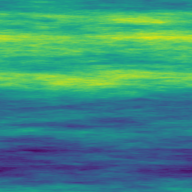
\includegraphics[interpolate=true,width=1.920000in,height=1.920000in]{random_field_anisoptropic-img0.png}}%
\end{pgfscope}%
\end{pgfpicture}%
\makeatother%
\endgroup%

    \caption{An anisotropic random field.}
    % \vspace{-10pt}
    \label{fig:ranom_field_anisotropic}
\end{wrapfigure}


% \begin{example}[White noise]
%     If the covariance is zero, we get white noise. If the covariance is one, the whole space has one degree of freedom so to speak and will have one random color.
% \end{example}
% We have a result by Loeve 
% \begin{theorem}[Loeve]
%     $k$ corresponds to the covariance of a Gaussian process if and only if $k$ is a positive semi-definite function, i.e.
%     \[
%         \sum_{i=0}^{n} \sum_{j=0}^{n} \alpha_{i} \alpha_{j} k(x_{i},x_{j}) \geq 0
%     \]
%     for all \( n \in \mathbb{N}, x_{i} \in \mathcal{X}, \alpha_{i} \in \mathbb{R} \).
% \end{theorem}

\begin{definition}[Strict Stationarity]\index{stationarity!strict}

    A stochastic process \( \{X(t)\}_{t \in T} \) is called \textit{strictly stationary} if for all \( k \geq 1 \), all \( (t_{1}, \dots t_{k}) \) in \( T^{k} \), the probability distribution of the random vector 
    \[
        (X(t_{1}+h), \dots, X(t_{k}+h))
    \]
    is independent of \( h \in T \), with \( h \in T \) such that \( t_{1}+h, \dots, t_{k}+h \in T\).
\end{definition}
%
\begin{definition}[Second Order Stochastic Process]\index{second order process}
    A measureable stochastic process \(\{X_{t}\}\) satisfying the condition
    \[
        \E\left[ \lvert X_{t} \rvert^2 \right] < \infty
    \]
    for all $t \in T$ is called a \textit{second order} stochastic process
\end{definition}
%
\begin{definition}[Weak Stationarity]\index{stationarity!weak}
    A second order stochastic process \(\{X_{t}\}\) with mean \(\mu_{X}(t)\) and covariance \( \Gamma_{X}(t,s) \) at \( t,s \in T \) is called \textit{weakly stationary}, if \( \mu_{X} \) is constant and \( \Gamma_{X}(t,s) \) is a function of \( t-s \) only.
\end{definition}

A process is called \textit{isotropic}\index{isotropy} if its covariance function \( \Gamma(t,s) \) is only a function of the distance \( \lvert t-s \rvert \). An example of when this condition is not met is shown in \cref{fig:ranom_field_anisotropic}

\begin{theorem}[Stationarity Equivalence]\index{stationarity!equivalence}
    For Gaussian processes on \( T = \mathbb{R}^{d} \), $d \in \mathbb{N}$ the concepts of weak and strict stationarity coincide.
\end{theorem}

\begin{proof}
    Strict stationarity implies weak stationarity trivially.
    For the other direction note that the mean and covariance functions completely characterize the finite dimensional distributions, since these are normal distributions.
\end{proof}
% (https://gpss.cc/gpss21/slides/Heinonen2021.pdf Page 10).
% \textcolor{red}{Do I want the following sentence?}
% In many physical domains random fields arise as sums of random waves. Their spacial interaction is understandably better characterized in the frequency domain. The following spectral theorem gives some insights into the connection between covariance functions and spectral densities. 
\begin{figure}[b]
    \centering
    %% Creator: Matplotlib, PGF backend
%%
%% To include the figure in your LaTeX document, write
%%   \input{<filename>.pgf}
%%
%% Make sure the required packages are loaded in your preamble
%%   \usepackage{pgf}
%%
%% Also ensure that all the required font packages are loaded; for instance,
%% the lmodern package is sometimes necessary when using math font.
%%   \usepackage{lmodern}
%%
%% Figures using additional raster images can only be included by \input if
%% they are in the same directory as the main LaTeX file. For loading figures
%% from other directories you can use the `import` package
%%   \usepackage{import}
%%
%% and then include the figures with
%%   \import{<path to file>}{<filename>.pgf}
%%
%% Matplotlib used the following preamble
%%   \def\mathdefault#1{#1}
%%   \everymath=\expandafter{\the\everymath\displaystyle}
%%   \usepackage[T1]{fontenc}
%%   \usepackage{siunitx}
%%   \usepackage{amssymb}
%%   \usepackage{amsmath}
%%   \makeatletter\@ifpackageloaded{underscore}{}{\usepackage[strings]{underscore}}\makeatother
%%
\begingroup%
\makeatletter%
\begin{pgfpicture}%
\pgfpathrectangle{\pgfpointorigin}{\pgfqpoint{1.736553in}{1.736553in}}%
\pgfusepath{use as bounding box, clip}%
\begin{pgfscope}%
\pgfsetbuttcap%
\pgfsetmiterjoin%
\definecolor{currentfill}{rgb}{1.000000,1.000000,1.000000}%
\pgfsetfillcolor{currentfill}%
\pgfsetlinewidth{0.000000pt}%
\definecolor{currentstroke}{rgb}{1.000000,1.000000,1.000000}%
\pgfsetstrokecolor{currentstroke}%
\pgfsetdash{}{0pt}%
\pgfpathmoveto{\pgfqpoint{0.000000in}{0.000000in}}%
\pgfpathlineto{\pgfqpoint{1.736553in}{0.000000in}}%
\pgfpathlineto{\pgfqpoint{1.736553in}{1.736553in}}%
\pgfpathlineto{\pgfqpoint{0.000000in}{1.736553in}}%
\pgfpathlineto{\pgfqpoint{0.000000in}{0.000000in}}%
\pgfpathclose%
\pgfusepath{fill}%
\end{pgfscope}%
\begin{pgfscope}%
\pgfsetbuttcap%
\pgfsetmiterjoin%
\definecolor{currentfill}{rgb}{1.000000,1.000000,1.000000}%
\pgfsetfillcolor{currentfill}%
\pgfsetlinewidth{0.000000pt}%
\definecolor{currentstroke}{rgb}{0.000000,0.000000,0.000000}%
\pgfsetstrokecolor{currentstroke}%
\pgfsetstrokeopacity{0.000000}%
\pgfsetdash{}{0pt}%
\pgfpathmoveto{\pgfqpoint{0.000000in}{0.000000in}}%
\pgfpathlineto{\pgfqpoint{1.736553in}{0.000000in}}%
\pgfpathlineto{\pgfqpoint{1.736553in}{1.736553in}}%
\pgfpathlineto{\pgfqpoint{0.000000in}{1.736553in}}%
\pgfpathlineto{\pgfqpoint{0.000000in}{0.000000in}}%
\pgfpathclose%
\pgfusepath{fill}%
\end{pgfscope}%
\begin{pgfscope}%
\pgfpathrectangle{\pgfqpoint{0.000000in}{0.000000in}}{\pgfqpoint{1.736553in}{1.736553in}}%
\pgfusepath{clip}%
\pgfsetrectcap%
\pgfsetroundjoin%
\pgfsetlinewidth{1.505625pt}%
\definecolor{currentstroke}{rgb}{1.000000,0.745098,0.043137}%
\pgfsetstrokecolor{currentstroke}%
\pgfsetdash{}{0pt}%
\pgfpathmoveto{\pgfqpoint{0.078934in}{0.597354in}}%
\pgfpathlineto{\pgfqpoint{0.094881in}{0.572819in}}%
\pgfpathlineto{\pgfqpoint{0.110827in}{0.523886in}}%
\pgfpathlineto{\pgfqpoint{0.126773in}{0.541530in}}%
\pgfpathlineto{\pgfqpoint{0.142719in}{0.555154in}}%
\pgfpathlineto{\pgfqpoint{0.158666in}{0.540930in}}%
\pgfpathlineto{\pgfqpoint{0.174612in}{0.423781in}}%
\pgfpathlineto{\pgfqpoint{0.190558in}{0.508756in}}%
\pgfpathlineto{\pgfqpoint{0.206505in}{0.383405in}}%
\pgfpathlineto{\pgfqpoint{0.222451in}{0.530588in}}%
\pgfpathlineto{\pgfqpoint{0.238397in}{0.507149in}}%
\pgfpathlineto{\pgfqpoint{0.254344in}{0.473371in}}%
\pgfpathlineto{\pgfqpoint{0.270290in}{0.447025in}}%
\pgfpathlineto{\pgfqpoint{0.286236in}{0.583090in}}%
\pgfpathlineto{\pgfqpoint{0.302183in}{0.540300in}}%
\pgfpathlineto{\pgfqpoint{0.318129in}{0.472239in}}%
\pgfpathlineto{\pgfqpoint{0.334075in}{0.466494in}}%
\pgfpathlineto{\pgfqpoint{0.350021in}{0.335508in}}%
\pgfpathlineto{\pgfqpoint{0.365968in}{0.372966in}}%
\pgfpathlineto{\pgfqpoint{0.381914in}{0.390692in}}%
\pgfpathlineto{\pgfqpoint{0.397860in}{0.388688in}}%
\pgfpathlineto{\pgfqpoint{0.413807in}{0.439716in}}%
\pgfpathlineto{\pgfqpoint{0.429753in}{0.443796in}}%
\pgfpathlineto{\pgfqpoint{0.445699in}{0.684593in}}%
\pgfpathlineto{\pgfqpoint{0.461646in}{0.677109in}}%
\pgfpathlineto{\pgfqpoint{0.477592in}{0.763308in}}%
\pgfpathlineto{\pgfqpoint{0.493538in}{0.803882in}}%
\pgfpathlineto{\pgfqpoint{0.509485in}{0.728573in}}%
\pgfpathlineto{\pgfqpoint{0.525431in}{0.658339in}}%
\pgfpathlineto{\pgfqpoint{0.541377in}{0.597465in}}%
\pgfpathlineto{\pgfqpoint{0.557323in}{0.678167in}}%
\pgfpathlineto{\pgfqpoint{0.573270in}{0.803808in}}%
\pgfpathlineto{\pgfqpoint{0.589216in}{0.957796in}}%
\pgfpathlineto{\pgfqpoint{0.605162in}{0.955543in}}%
\pgfpathlineto{\pgfqpoint{0.621109in}{0.944501in}}%
\pgfpathlineto{\pgfqpoint{0.637055in}{0.959784in}}%
\pgfpathlineto{\pgfqpoint{0.653001in}{0.858692in}}%
\pgfpathlineto{\pgfqpoint{0.668948in}{0.816514in}}%
\pgfpathlineto{\pgfqpoint{0.684894in}{0.743290in}}%
\pgfpathlineto{\pgfqpoint{0.700840in}{0.884732in}}%
\pgfpathlineto{\pgfqpoint{0.716787in}{0.910608in}}%
\pgfpathlineto{\pgfqpoint{0.732733in}{0.924974in}}%
\pgfpathlineto{\pgfqpoint{0.748679in}{0.981079in}}%
\pgfpathlineto{\pgfqpoint{0.764625in}{0.975342in}}%
\pgfpathlineto{\pgfqpoint{0.780572in}{1.054578in}}%
\pgfpathlineto{\pgfqpoint{0.796518in}{0.931943in}}%
\pgfpathlineto{\pgfqpoint{0.812464in}{0.987974in}}%
\pgfpathlineto{\pgfqpoint{0.828411in}{0.899395in}}%
\pgfpathlineto{\pgfqpoint{0.844357in}{0.884652in}}%
\pgfpathlineto{\pgfqpoint{0.860303in}{0.952260in}}%
\pgfpathlineto{\pgfqpoint{0.876250in}{0.921470in}}%
\pgfpathlineto{\pgfqpoint{0.892196in}{0.952062in}}%
\pgfpathlineto{\pgfqpoint{0.908142in}{0.876299in}}%
\pgfpathlineto{\pgfqpoint{0.924089in}{0.824040in}}%
\pgfpathlineto{\pgfqpoint{0.940035in}{0.824115in}}%
\pgfpathlineto{\pgfqpoint{0.955981in}{0.729242in}}%
\pgfpathlineto{\pgfqpoint{0.971928in}{0.680483in}}%
\pgfpathlineto{\pgfqpoint{0.987874in}{0.643527in}}%
\pgfpathlineto{\pgfqpoint{1.003820in}{0.773837in}}%
\pgfpathlineto{\pgfqpoint{1.019766in}{0.782563in}}%
\pgfpathlineto{\pgfqpoint{1.035713in}{0.707945in}}%
\pgfpathlineto{\pgfqpoint{1.051659in}{0.671844in}}%
\pgfpathlineto{\pgfqpoint{1.067605in}{0.678028in}}%
\pgfpathlineto{\pgfqpoint{1.083552in}{0.714294in}}%
\pgfpathlineto{\pgfqpoint{1.099498in}{0.709146in}}%
\pgfpathlineto{\pgfqpoint{1.115444in}{0.594807in}}%
\pgfpathlineto{\pgfqpoint{1.131391in}{0.443070in}}%
\pgfpathlineto{\pgfqpoint{1.147337in}{0.422680in}}%
\pgfpathlineto{\pgfqpoint{1.163283in}{0.605446in}}%
\pgfpathlineto{\pgfqpoint{1.179230in}{0.434094in}}%
\pgfpathlineto{\pgfqpoint{1.195176in}{0.236813in}}%
\pgfpathlineto{\pgfqpoint{1.211122in}{0.217593in}}%
\pgfpathlineto{\pgfqpoint{1.227068in}{0.157423in}}%
\pgfpathlineto{\pgfqpoint{1.243015in}{0.412849in}}%
\pgfpathlineto{\pgfqpoint{1.258961in}{0.500857in}}%
\pgfpathlineto{\pgfqpoint{1.274907in}{0.560561in}}%
\pgfpathlineto{\pgfqpoint{1.290854in}{0.502796in}}%
\pgfpathlineto{\pgfqpoint{1.306800in}{0.376484in}}%
\pgfpathlineto{\pgfqpoint{1.322746in}{0.258868in}}%
\pgfpathlineto{\pgfqpoint{1.338693in}{0.273022in}}%
\pgfpathlineto{\pgfqpoint{1.354639in}{0.466646in}}%
\pgfpathlineto{\pgfqpoint{1.370585in}{0.582374in}}%
\pgfpathlineto{\pgfqpoint{1.386532in}{0.645853in}}%
\pgfpathlineto{\pgfqpoint{1.402478in}{0.828005in}}%
\pgfpathlineto{\pgfqpoint{1.418424in}{0.858518in}}%
\pgfpathlineto{\pgfqpoint{1.434370in}{0.803388in}}%
\pgfpathlineto{\pgfqpoint{1.450317in}{0.779115in}}%
\pgfpathlineto{\pgfqpoint{1.466263in}{0.870217in}}%
\pgfpathlineto{\pgfqpoint{1.482209in}{0.876953in}}%
\pgfpathlineto{\pgfqpoint{1.498156in}{0.905919in}}%
\pgfpathlineto{\pgfqpoint{1.514102in}{0.872603in}}%
\pgfpathlineto{\pgfqpoint{1.530048in}{0.914796in}}%
\pgfpathlineto{\pgfqpoint{1.545995in}{1.115195in}}%
\pgfpathlineto{\pgfqpoint{1.561941in}{1.288556in}}%
\pgfpathlineto{\pgfqpoint{1.577887in}{1.138474in}}%
\pgfpathlineto{\pgfqpoint{1.593834in}{1.322962in}}%
\pgfpathlineto{\pgfqpoint{1.609780in}{1.409074in}}%
\pgfpathlineto{\pgfqpoint{1.625726in}{1.501723in}}%
\pgfpathlineto{\pgfqpoint{1.641672in}{1.508594in}}%
\pgfpathlineto{\pgfqpoint{1.657619in}{1.421900in}}%
\pgfusepath{stroke}%
\end{pgfscope}%
\begin{pgfscope}%
\pgfpathrectangle{\pgfqpoint{0.000000in}{0.000000in}}{\pgfqpoint{1.736553in}{1.736553in}}%
\pgfusepath{clip}%
\pgfsetrectcap%
\pgfsetroundjoin%
\pgfsetlinewidth{1.505625pt}%
\definecolor{currentstroke}{rgb}{0.984314,0.337255,0.027451}%
\pgfsetstrokecolor{currentstroke}%
\pgfsetdash{}{0pt}%
\pgfpathmoveto{\pgfqpoint{0.078934in}{0.798942in}}%
\pgfpathlineto{\pgfqpoint{0.094881in}{0.920122in}}%
\pgfpathlineto{\pgfqpoint{0.110827in}{0.833388in}}%
\pgfpathlineto{\pgfqpoint{0.126773in}{0.934435in}}%
\pgfpathlineto{\pgfqpoint{0.142719in}{0.927345in}}%
\pgfpathlineto{\pgfqpoint{0.158666in}{1.112003in}}%
\pgfpathlineto{\pgfqpoint{0.174612in}{1.191900in}}%
\pgfpathlineto{\pgfqpoint{0.190558in}{1.229548in}}%
\pgfpathlineto{\pgfqpoint{0.206505in}{1.180584in}}%
\pgfpathlineto{\pgfqpoint{0.222451in}{1.128798in}}%
\pgfpathlineto{\pgfqpoint{0.238397in}{1.305087in}}%
\pgfpathlineto{\pgfqpoint{0.254344in}{1.269954in}}%
\pgfpathlineto{\pgfqpoint{0.270290in}{1.185360in}}%
\pgfpathlineto{\pgfqpoint{0.286236in}{1.271441in}}%
\pgfpathlineto{\pgfqpoint{0.302183in}{1.088432in}}%
\pgfpathlineto{\pgfqpoint{0.318129in}{1.057050in}}%
\pgfpathlineto{\pgfqpoint{0.334075in}{0.915948in}}%
\pgfpathlineto{\pgfqpoint{0.350021in}{1.031808in}}%
\pgfpathlineto{\pgfqpoint{0.365968in}{0.972760in}}%
\pgfpathlineto{\pgfqpoint{0.381914in}{1.051939in}}%
\pgfpathlineto{\pgfqpoint{0.397860in}{1.097358in}}%
\pgfpathlineto{\pgfqpoint{0.413807in}{1.105391in}}%
\pgfpathlineto{\pgfqpoint{0.429753in}{0.911435in}}%
\pgfpathlineto{\pgfqpoint{0.445699in}{1.043790in}}%
\pgfpathlineto{\pgfqpoint{0.461646in}{0.987670in}}%
\pgfpathlineto{\pgfqpoint{0.477592in}{0.899375in}}%
\pgfpathlineto{\pgfqpoint{0.493538in}{0.765688in}}%
\pgfpathlineto{\pgfqpoint{0.509485in}{0.839864in}}%
\pgfpathlineto{\pgfqpoint{0.525431in}{0.876479in}}%
\pgfpathlineto{\pgfqpoint{0.541377in}{0.887176in}}%
\pgfpathlineto{\pgfqpoint{0.557323in}{0.841167in}}%
\pgfpathlineto{\pgfqpoint{0.573270in}{0.835870in}}%
\pgfpathlineto{\pgfqpoint{0.589216in}{0.821962in}}%
\pgfpathlineto{\pgfqpoint{0.605162in}{0.933747in}}%
\pgfpathlineto{\pgfqpoint{0.621109in}{1.034096in}}%
\pgfpathlineto{\pgfqpoint{0.637055in}{1.079633in}}%
\pgfpathlineto{\pgfqpoint{0.653001in}{1.063012in}}%
\pgfpathlineto{\pgfqpoint{0.668948in}{1.252042in}}%
\pgfpathlineto{\pgfqpoint{0.684894in}{1.219583in}}%
\pgfpathlineto{\pgfqpoint{0.700840in}{1.087553in}}%
\pgfpathlineto{\pgfqpoint{0.716787in}{0.986535in}}%
\pgfpathlineto{\pgfqpoint{0.732733in}{0.860421in}}%
\pgfpathlineto{\pgfqpoint{0.748679in}{0.699626in}}%
\pgfpathlineto{\pgfqpoint{0.764625in}{0.679939in}}%
\pgfpathlineto{\pgfqpoint{0.780572in}{0.564763in}}%
\pgfpathlineto{\pgfqpoint{0.796518in}{0.515891in}}%
\pgfpathlineto{\pgfqpoint{0.812464in}{0.499956in}}%
\pgfpathlineto{\pgfqpoint{0.828411in}{0.376758in}}%
\pgfpathlineto{\pgfqpoint{0.844357in}{0.236002in}}%
\pgfpathlineto{\pgfqpoint{0.860303in}{0.212152in}}%
\pgfpathlineto{\pgfqpoint{0.876250in}{0.129080in}}%
\pgfpathlineto{\pgfqpoint{0.892196in}{0.114616in}}%
\pgfpathlineto{\pgfqpoint{0.908142in}{0.146088in}}%
\pgfpathlineto{\pgfqpoint{0.924089in}{0.078934in}}%
\pgfpathlineto{\pgfqpoint{0.940035in}{0.102285in}}%
\pgfpathlineto{\pgfqpoint{0.955981in}{0.198688in}}%
\pgfpathlineto{\pgfqpoint{0.971928in}{0.226882in}}%
\pgfpathlineto{\pgfqpoint{0.987874in}{0.314157in}}%
\pgfpathlineto{\pgfqpoint{1.003820in}{0.242413in}}%
\pgfpathlineto{\pgfqpoint{1.019766in}{0.312075in}}%
\pgfpathlineto{\pgfqpoint{1.035713in}{0.315072in}}%
\pgfpathlineto{\pgfqpoint{1.051659in}{0.213218in}}%
\pgfpathlineto{\pgfqpoint{1.067605in}{0.125709in}}%
\pgfpathlineto{\pgfqpoint{1.083552in}{0.147907in}}%
\pgfpathlineto{\pgfqpoint{1.099498in}{0.352521in}}%
\pgfpathlineto{\pgfqpoint{1.115444in}{0.258638in}}%
\pgfpathlineto{\pgfqpoint{1.131391in}{0.284158in}}%
\pgfpathlineto{\pgfqpoint{1.147337in}{0.287550in}}%
\pgfpathlineto{\pgfqpoint{1.163283in}{0.329746in}}%
\pgfpathlineto{\pgfqpoint{1.179230in}{0.316850in}}%
\pgfpathlineto{\pgfqpoint{1.195176in}{0.387564in}}%
\pgfpathlineto{\pgfqpoint{1.211122in}{0.321173in}}%
\pgfpathlineto{\pgfqpoint{1.227068in}{0.394013in}}%
\pgfpathlineto{\pgfqpoint{1.243015in}{0.705268in}}%
\pgfpathlineto{\pgfqpoint{1.258961in}{0.623876in}}%
\pgfpathlineto{\pgfqpoint{1.274907in}{0.786438in}}%
\pgfpathlineto{\pgfqpoint{1.290854in}{0.804252in}}%
\pgfpathlineto{\pgfqpoint{1.306800in}{0.722137in}}%
\pgfpathlineto{\pgfqpoint{1.322746in}{0.778773in}}%
\pgfpathlineto{\pgfqpoint{1.338693in}{0.914040in}}%
\pgfpathlineto{\pgfqpoint{1.354639in}{1.023506in}}%
\pgfpathlineto{\pgfqpoint{1.370585in}{0.935107in}}%
\pgfpathlineto{\pgfqpoint{1.386532in}{0.875209in}}%
\pgfpathlineto{\pgfqpoint{1.402478in}{0.860306in}}%
\pgfpathlineto{\pgfqpoint{1.418424in}{0.902711in}}%
\pgfpathlineto{\pgfqpoint{1.434370in}{0.870994in}}%
\pgfpathlineto{\pgfqpoint{1.450317in}{0.773331in}}%
\pgfpathlineto{\pgfqpoint{1.466263in}{0.712112in}}%
\pgfpathlineto{\pgfqpoint{1.482209in}{0.834711in}}%
\pgfpathlineto{\pgfqpoint{1.498156in}{0.733362in}}%
\pgfpathlineto{\pgfqpoint{1.514102in}{0.589783in}}%
\pgfpathlineto{\pgfqpoint{1.530048in}{0.416617in}}%
\pgfpathlineto{\pgfqpoint{1.545995in}{0.529055in}}%
\pgfpathlineto{\pgfqpoint{1.561941in}{0.515840in}}%
\pgfpathlineto{\pgfqpoint{1.577887in}{0.540384in}}%
\pgfpathlineto{\pgfqpoint{1.593834in}{0.664321in}}%
\pgfpathlineto{\pgfqpoint{1.609780in}{0.726687in}}%
\pgfpathlineto{\pgfqpoint{1.625726in}{0.826325in}}%
\pgfpathlineto{\pgfqpoint{1.641672in}{0.798123in}}%
\pgfpathlineto{\pgfqpoint{1.657619in}{0.859115in}}%
\pgfusepath{stroke}%
\end{pgfscope}%
\begin{pgfscope}%
\pgfpathrectangle{\pgfqpoint{0.000000in}{0.000000in}}{\pgfqpoint{1.736553in}{1.736553in}}%
\pgfusepath{clip}%
\pgfsetrectcap%
\pgfsetroundjoin%
\pgfsetlinewidth{1.505625pt}%
\definecolor{currentstroke}{rgb}{1.000000,0.000000,0.431373}%
\pgfsetstrokecolor{currentstroke}%
\pgfsetdash{}{0pt}%
\pgfpathmoveto{\pgfqpoint{0.078934in}{0.914283in}}%
\pgfpathlineto{\pgfqpoint{0.094881in}{0.759890in}}%
\pgfpathlineto{\pgfqpoint{0.110827in}{0.762467in}}%
\pgfpathlineto{\pgfqpoint{0.126773in}{0.810402in}}%
\pgfpathlineto{\pgfqpoint{0.142719in}{0.804461in}}%
\pgfpathlineto{\pgfqpoint{0.158666in}{0.748231in}}%
\pgfpathlineto{\pgfqpoint{0.174612in}{0.752133in}}%
\pgfpathlineto{\pgfqpoint{0.190558in}{0.847007in}}%
\pgfpathlineto{\pgfqpoint{0.206505in}{0.795824in}}%
\pgfpathlineto{\pgfqpoint{0.222451in}{0.864590in}}%
\pgfpathlineto{\pgfqpoint{0.238397in}{0.845323in}}%
\pgfpathlineto{\pgfqpoint{0.254344in}{0.949608in}}%
\pgfpathlineto{\pgfqpoint{0.270290in}{1.050594in}}%
\pgfpathlineto{\pgfqpoint{0.286236in}{1.148055in}}%
\pgfpathlineto{\pgfqpoint{0.302183in}{1.091956in}}%
\pgfpathlineto{\pgfqpoint{0.318129in}{0.945966in}}%
\pgfpathlineto{\pgfqpoint{0.334075in}{1.035360in}}%
\pgfpathlineto{\pgfqpoint{0.350021in}{1.140232in}}%
\pgfpathlineto{\pgfqpoint{0.365968in}{1.142261in}}%
\pgfpathlineto{\pgfqpoint{0.381914in}{1.215936in}}%
\pgfpathlineto{\pgfqpoint{0.397860in}{1.238661in}}%
\pgfpathlineto{\pgfqpoint{0.413807in}{1.198636in}}%
\pgfpathlineto{\pgfqpoint{0.429753in}{1.184471in}}%
\pgfpathlineto{\pgfqpoint{0.445699in}{1.171784in}}%
\pgfpathlineto{\pgfqpoint{0.461646in}{1.144104in}}%
\pgfpathlineto{\pgfqpoint{0.477592in}{1.080395in}}%
\pgfpathlineto{\pgfqpoint{0.493538in}{1.028049in}}%
\pgfpathlineto{\pgfqpoint{0.509485in}{0.988106in}}%
\pgfpathlineto{\pgfqpoint{0.525431in}{1.019079in}}%
\pgfpathlineto{\pgfqpoint{0.541377in}{1.159316in}}%
\pgfpathlineto{\pgfqpoint{0.557323in}{1.164618in}}%
\pgfpathlineto{\pgfqpoint{0.573270in}{1.096027in}}%
\pgfpathlineto{\pgfqpoint{0.589216in}{1.062091in}}%
\pgfpathlineto{\pgfqpoint{0.605162in}{1.107313in}}%
\pgfpathlineto{\pgfqpoint{0.621109in}{1.260780in}}%
\pgfpathlineto{\pgfqpoint{0.637055in}{1.310391in}}%
\pgfpathlineto{\pgfqpoint{0.653001in}{1.255074in}}%
\pgfpathlineto{\pgfqpoint{0.668948in}{1.126837in}}%
\pgfpathlineto{\pgfqpoint{0.684894in}{1.130008in}}%
\pgfpathlineto{\pgfqpoint{0.700840in}{1.224745in}}%
\pgfpathlineto{\pgfqpoint{0.716787in}{1.250641in}}%
\pgfpathlineto{\pgfqpoint{0.732733in}{1.172528in}}%
\pgfpathlineto{\pgfqpoint{0.748679in}{1.260710in}}%
\pgfpathlineto{\pgfqpoint{0.764625in}{1.214870in}}%
\pgfpathlineto{\pgfqpoint{0.780572in}{1.330452in}}%
\pgfpathlineto{\pgfqpoint{0.796518in}{1.484145in}}%
\pgfpathlineto{\pgfqpoint{0.812464in}{1.324183in}}%
\pgfpathlineto{\pgfqpoint{0.828411in}{1.339245in}}%
\pgfpathlineto{\pgfqpoint{0.844357in}{1.317734in}}%
\pgfpathlineto{\pgfqpoint{0.860303in}{1.121460in}}%
\pgfpathlineto{\pgfqpoint{0.876250in}{1.185619in}}%
\pgfpathlineto{\pgfqpoint{0.892196in}{1.278935in}}%
\pgfpathlineto{\pgfqpoint{0.908142in}{1.331868in}}%
\pgfpathlineto{\pgfqpoint{0.924089in}{1.344835in}}%
\pgfpathlineto{\pgfqpoint{0.940035in}{1.307172in}}%
\pgfpathlineto{\pgfqpoint{0.955981in}{1.367194in}}%
\pgfpathlineto{\pgfqpoint{0.971928in}{1.267012in}}%
\pgfpathlineto{\pgfqpoint{0.987874in}{1.287025in}}%
\pgfpathlineto{\pgfqpoint{1.003820in}{1.158077in}}%
\pgfpathlineto{\pgfqpoint{1.019766in}{1.206715in}}%
\pgfpathlineto{\pgfqpoint{1.035713in}{1.106788in}}%
\pgfpathlineto{\pgfqpoint{1.051659in}{1.229908in}}%
\pgfpathlineto{\pgfqpoint{1.067605in}{1.312622in}}%
\pgfpathlineto{\pgfqpoint{1.083552in}{1.249083in}}%
\pgfpathlineto{\pgfqpoint{1.099498in}{1.299443in}}%
\pgfpathlineto{\pgfqpoint{1.115444in}{1.243921in}}%
\pgfpathlineto{\pgfqpoint{1.131391in}{1.229226in}}%
\pgfpathlineto{\pgfqpoint{1.147337in}{1.070590in}}%
\pgfpathlineto{\pgfqpoint{1.163283in}{1.002885in}}%
\pgfpathlineto{\pgfqpoint{1.179230in}{0.858755in}}%
\pgfpathlineto{\pgfqpoint{1.195176in}{0.885790in}}%
\pgfpathlineto{\pgfqpoint{1.211122in}{0.650841in}}%
\pgfpathlineto{\pgfqpoint{1.227068in}{0.780285in}}%
\pgfpathlineto{\pgfqpoint{1.243015in}{0.895476in}}%
\pgfpathlineto{\pgfqpoint{1.258961in}{0.701046in}}%
\pgfpathlineto{\pgfqpoint{1.274907in}{0.816009in}}%
\pgfpathlineto{\pgfqpoint{1.290854in}{0.850389in}}%
\pgfpathlineto{\pgfqpoint{1.306800in}{0.872423in}}%
\pgfpathlineto{\pgfqpoint{1.322746in}{0.862225in}}%
\pgfpathlineto{\pgfqpoint{1.338693in}{0.932260in}}%
\pgfpathlineto{\pgfqpoint{1.354639in}{0.837747in}}%
\pgfpathlineto{\pgfqpoint{1.370585in}{0.858652in}}%
\pgfpathlineto{\pgfqpoint{1.386532in}{0.689382in}}%
\pgfpathlineto{\pgfqpoint{1.402478in}{0.722323in}}%
\pgfpathlineto{\pgfqpoint{1.418424in}{0.744268in}}%
\pgfpathlineto{\pgfqpoint{1.434370in}{0.835945in}}%
\pgfpathlineto{\pgfqpoint{1.450317in}{0.933643in}}%
\pgfpathlineto{\pgfqpoint{1.466263in}{0.895979in}}%
\pgfpathlineto{\pgfqpoint{1.482209in}{0.907833in}}%
\pgfpathlineto{\pgfqpoint{1.498156in}{0.966746in}}%
\pgfpathlineto{\pgfqpoint{1.514102in}{0.954813in}}%
\pgfpathlineto{\pgfqpoint{1.530048in}{0.949608in}}%
\pgfpathlineto{\pgfqpoint{1.545995in}{1.022315in}}%
\pgfpathlineto{\pgfqpoint{1.561941in}{1.197833in}}%
\pgfpathlineto{\pgfqpoint{1.577887in}{1.105779in}}%
\pgfpathlineto{\pgfqpoint{1.593834in}{1.102393in}}%
\pgfpathlineto{\pgfqpoint{1.609780in}{1.181239in}}%
\pgfpathlineto{\pgfqpoint{1.625726in}{1.119112in}}%
\pgfpathlineto{\pgfqpoint{1.641672in}{1.345942in}}%
\pgfpathlineto{\pgfqpoint{1.657619in}{1.180953in}}%
\pgfusepath{stroke}%
\end{pgfscope}%
\begin{pgfscope}%
\pgfpathrectangle{\pgfqpoint{0.000000in}{0.000000in}}{\pgfqpoint{1.736553in}{1.736553in}}%
\pgfusepath{clip}%
\pgfsetrectcap%
\pgfsetroundjoin%
\pgfsetlinewidth{1.505625pt}%
\definecolor{currentstroke}{rgb}{0.513725,0.219608,0.925490}%
\pgfsetstrokecolor{currentstroke}%
\pgfsetdash{}{0pt}%
\pgfpathmoveto{\pgfqpoint{0.078934in}{0.801081in}}%
\pgfpathlineto{\pgfqpoint{0.094881in}{0.856508in}}%
\pgfpathlineto{\pgfqpoint{0.110827in}{0.703491in}}%
\pgfpathlineto{\pgfqpoint{0.126773in}{0.777527in}}%
\pgfpathlineto{\pgfqpoint{0.142719in}{0.880366in}}%
\pgfpathlineto{\pgfqpoint{0.158666in}{1.015537in}}%
\pgfpathlineto{\pgfqpoint{0.174612in}{1.029396in}}%
\pgfpathlineto{\pgfqpoint{0.190558in}{1.011373in}}%
\pgfpathlineto{\pgfqpoint{0.206505in}{1.126453in}}%
\pgfpathlineto{\pgfqpoint{0.222451in}{1.096157in}}%
\pgfpathlineto{\pgfqpoint{0.238397in}{1.200942in}}%
\pgfpathlineto{\pgfqpoint{0.254344in}{1.188402in}}%
\pgfpathlineto{\pgfqpoint{0.270290in}{1.174694in}}%
\pgfpathlineto{\pgfqpoint{0.286236in}{1.153127in}}%
\pgfpathlineto{\pgfqpoint{0.302183in}{1.042623in}}%
\pgfpathlineto{\pgfqpoint{0.318129in}{1.264589in}}%
\pgfpathlineto{\pgfqpoint{0.334075in}{1.161412in}}%
\pgfpathlineto{\pgfqpoint{0.350021in}{1.097906in}}%
\pgfpathlineto{\pgfqpoint{0.365968in}{0.887998in}}%
\pgfpathlineto{\pgfqpoint{0.381914in}{0.945005in}}%
\pgfpathlineto{\pgfqpoint{0.397860in}{1.015138in}}%
\pgfpathlineto{\pgfqpoint{0.413807in}{1.098870in}}%
\pgfpathlineto{\pgfqpoint{0.429753in}{1.008025in}}%
\pgfpathlineto{\pgfqpoint{0.445699in}{0.970493in}}%
\pgfpathlineto{\pgfqpoint{0.461646in}{0.803162in}}%
\pgfpathlineto{\pgfqpoint{0.477592in}{0.806862in}}%
\pgfpathlineto{\pgfqpoint{0.493538in}{0.755046in}}%
\pgfpathlineto{\pgfqpoint{0.509485in}{0.955592in}}%
\pgfpathlineto{\pgfqpoint{0.525431in}{0.919179in}}%
\pgfpathlineto{\pgfqpoint{0.541377in}{0.829906in}}%
\pgfpathlineto{\pgfqpoint{0.557323in}{0.771184in}}%
\pgfpathlineto{\pgfqpoint{0.573270in}{0.725325in}}%
\pgfpathlineto{\pgfqpoint{0.589216in}{0.609031in}}%
\pgfpathlineto{\pgfqpoint{0.605162in}{0.736792in}}%
\pgfpathlineto{\pgfqpoint{0.621109in}{0.849551in}}%
\pgfpathlineto{\pgfqpoint{0.637055in}{0.956293in}}%
\pgfpathlineto{\pgfqpoint{0.653001in}{0.983325in}}%
\pgfpathlineto{\pgfqpoint{0.668948in}{0.894786in}}%
\pgfpathlineto{\pgfqpoint{0.684894in}{0.976994in}}%
\pgfpathlineto{\pgfqpoint{0.700840in}{0.991664in}}%
\pgfpathlineto{\pgfqpoint{0.716787in}{1.137180in}}%
\pgfpathlineto{\pgfqpoint{0.732733in}{1.189801in}}%
\pgfpathlineto{\pgfqpoint{0.748679in}{1.252874in}}%
\pgfpathlineto{\pgfqpoint{0.764625in}{1.341866in}}%
\pgfpathlineto{\pgfqpoint{0.780572in}{1.403199in}}%
\pgfpathlineto{\pgfqpoint{0.796518in}{1.464474in}}%
\pgfpathlineto{\pgfqpoint{0.812464in}{1.401630in}}%
\pgfpathlineto{\pgfqpoint{0.828411in}{1.440726in}}%
\pgfpathlineto{\pgfqpoint{0.844357in}{1.356706in}}%
\pgfpathlineto{\pgfqpoint{0.860303in}{1.326471in}}%
\pgfpathlineto{\pgfqpoint{0.876250in}{1.329010in}}%
\pgfpathlineto{\pgfqpoint{0.892196in}{1.398592in}}%
\pgfpathlineto{\pgfqpoint{0.908142in}{1.397526in}}%
\pgfpathlineto{\pgfqpoint{0.924089in}{1.315933in}}%
\pgfpathlineto{\pgfqpoint{0.940035in}{1.387170in}}%
\pgfpathlineto{\pgfqpoint{0.955981in}{1.335719in}}%
\pgfpathlineto{\pgfqpoint{0.971928in}{1.408417in}}%
\pgfpathlineto{\pgfqpoint{0.987874in}{1.415123in}}%
\pgfpathlineto{\pgfqpoint{1.003820in}{1.529465in}}%
\pgfpathlineto{\pgfqpoint{1.019766in}{1.606603in}}%
\pgfpathlineto{\pgfqpoint{1.035713in}{1.438392in}}%
\pgfpathlineto{\pgfqpoint{1.051659in}{1.513729in}}%
\pgfpathlineto{\pgfqpoint{1.067605in}{1.617104in}}%
\pgfpathlineto{\pgfqpoint{1.083552in}{1.552834in}}%
\pgfpathlineto{\pgfqpoint{1.099498in}{1.477076in}}%
\pgfpathlineto{\pgfqpoint{1.115444in}{1.486820in}}%
\pgfpathlineto{\pgfqpoint{1.131391in}{1.530801in}}%
\pgfpathlineto{\pgfqpoint{1.147337in}{1.526768in}}%
\pgfpathlineto{\pgfqpoint{1.163283in}{1.451859in}}%
\pgfpathlineto{\pgfqpoint{1.179230in}{1.419316in}}%
\pgfpathlineto{\pgfqpoint{1.195176in}{1.470831in}}%
\pgfpathlineto{\pgfqpoint{1.211122in}{1.479916in}}%
\pgfpathlineto{\pgfqpoint{1.227068in}{1.481475in}}%
\pgfpathlineto{\pgfqpoint{1.243015in}{1.487022in}}%
\pgfpathlineto{\pgfqpoint{1.258961in}{1.469063in}}%
\pgfpathlineto{\pgfqpoint{1.274907in}{1.566939in}}%
\pgfpathlineto{\pgfqpoint{1.290854in}{1.657619in}}%
\pgfpathlineto{\pgfqpoint{1.306800in}{1.564765in}}%
\pgfpathlineto{\pgfqpoint{1.322746in}{1.520723in}}%
\pgfpathlineto{\pgfqpoint{1.338693in}{1.485344in}}%
\pgfpathlineto{\pgfqpoint{1.354639in}{1.414083in}}%
\pgfpathlineto{\pgfqpoint{1.370585in}{1.564525in}}%
\pgfpathlineto{\pgfqpoint{1.386532in}{1.531984in}}%
\pgfpathlineto{\pgfqpoint{1.402478in}{1.512745in}}%
\pgfpathlineto{\pgfqpoint{1.418424in}{1.360463in}}%
\pgfpathlineto{\pgfqpoint{1.434370in}{1.374369in}}%
\pgfpathlineto{\pgfqpoint{1.450317in}{1.528217in}}%
\pgfpathlineto{\pgfqpoint{1.466263in}{1.531270in}}%
\pgfpathlineto{\pgfqpoint{1.482209in}{1.618586in}}%
\pgfpathlineto{\pgfqpoint{1.498156in}{1.389914in}}%
\pgfpathlineto{\pgfqpoint{1.514102in}{1.428816in}}%
\pgfpathlineto{\pgfqpoint{1.530048in}{1.380128in}}%
\pgfpathlineto{\pgfqpoint{1.545995in}{1.396314in}}%
\pgfpathlineto{\pgfqpoint{1.561941in}{1.532668in}}%
\pgfpathlineto{\pgfqpoint{1.577887in}{1.532761in}}%
\pgfpathlineto{\pgfqpoint{1.593834in}{1.520029in}}%
\pgfpathlineto{\pgfqpoint{1.609780in}{1.418517in}}%
\pgfpathlineto{\pgfqpoint{1.625726in}{1.308956in}}%
\pgfpathlineto{\pgfqpoint{1.641672in}{1.325702in}}%
\pgfpathlineto{\pgfqpoint{1.657619in}{1.165301in}}%
\pgfusepath{stroke}%
\end{pgfscope}%
\end{pgfpicture}%
\makeatother%
\endgroup%

    %% Creator: Matplotlib, PGF backend
%%
%% To include the figure in your LaTeX document, write
%%   \input{<filename>.pgf}
%%
%% Make sure the required packages are loaded in your preamble
%%   \usepackage{pgf}
%%
%% Also ensure that all the required font packages are loaded; for instance,
%% the lmodern package is sometimes necessary when using math font.
%%   \usepackage{lmodern}
%%
%% Figures using additional raster images can only be included by \input if
%% they are in the same directory as the main LaTeX file. For loading figures
%% from other directories you can use the `import` package
%%   \usepackage{import}
%%
%% and then include the figures with
%%   \import{<path to file>}{<filename>.pgf}
%%
%% Matplotlib used the following preamble
%%   \def\mathdefault#1{#1}
%%   \everymath=\expandafter{\the\everymath\displaystyle}
%%   \usepackage[T1]{fontenc}
%%   \usepackage{siunitx}
%%   \usepackage{amssymb}
%%   \usepackage{amsmath}
%%   \makeatletter\@ifpackageloaded{underscore}{}{\usepackage[strings]{underscore}}\makeatother
%%
\begingroup%
\makeatletter%
\begin{pgfpicture}%
\pgfpathrectangle{\pgfpointorigin}{\pgfqpoint{1.736553in}{1.736553in}}%
\pgfusepath{use as bounding box, clip}%
\begin{pgfscope}%
\pgfsetbuttcap%
\pgfsetmiterjoin%
\definecolor{currentfill}{rgb}{1.000000,1.000000,1.000000}%
\pgfsetfillcolor{currentfill}%
\pgfsetlinewidth{0.000000pt}%
\definecolor{currentstroke}{rgb}{1.000000,1.000000,1.000000}%
\pgfsetstrokecolor{currentstroke}%
\pgfsetdash{}{0pt}%
\pgfpathmoveto{\pgfqpoint{0.000000in}{0.000000in}}%
\pgfpathlineto{\pgfqpoint{1.736553in}{0.000000in}}%
\pgfpathlineto{\pgfqpoint{1.736553in}{1.736553in}}%
\pgfpathlineto{\pgfqpoint{0.000000in}{1.736553in}}%
\pgfpathlineto{\pgfqpoint{0.000000in}{0.000000in}}%
\pgfpathclose%
\pgfusepath{fill}%
\end{pgfscope}%
\begin{pgfscope}%
\pgfsetbuttcap%
\pgfsetmiterjoin%
\definecolor{currentfill}{rgb}{1.000000,1.000000,1.000000}%
\pgfsetfillcolor{currentfill}%
\pgfsetlinewidth{0.000000pt}%
\definecolor{currentstroke}{rgb}{0.000000,0.000000,0.000000}%
\pgfsetstrokecolor{currentstroke}%
\pgfsetstrokeopacity{0.000000}%
\pgfsetdash{}{0pt}%
\pgfpathmoveto{\pgfqpoint{0.000000in}{0.000000in}}%
\pgfpathlineto{\pgfqpoint{1.736553in}{0.000000in}}%
\pgfpathlineto{\pgfqpoint{1.736553in}{1.736553in}}%
\pgfpathlineto{\pgfqpoint{0.000000in}{1.736553in}}%
\pgfpathlineto{\pgfqpoint{0.000000in}{0.000000in}}%
\pgfpathclose%
\pgfusepath{fill}%
\end{pgfscope}%
\begin{pgfscope}%
\pgfpathrectangle{\pgfqpoint{0.000000in}{0.000000in}}{\pgfqpoint{1.736553in}{1.736553in}}%
\pgfusepath{clip}%
\pgfsetrectcap%
\pgfsetroundjoin%
\pgfsetlinewidth{1.505625pt}%
\definecolor{currentstroke}{rgb}{1.000000,0.745098,0.043137}%
\pgfsetstrokecolor{currentstroke}%
\pgfsetdash{}{0pt}%
\pgfpathmoveto{\pgfqpoint{0.078934in}{0.179801in}}%
\pgfpathlineto{\pgfqpoint{0.094881in}{0.195062in}}%
\pgfpathlineto{\pgfqpoint{0.110827in}{0.216311in}}%
\pgfpathlineto{\pgfqpoint{0.126773in}{0.218788in}}%
\pgfpathlineto{\pgfqpoint{0.142719in}{0.220642in}}%
\pgfpathlineto{\pgfqpoint{0.158666in}{0.233616in}}%
\pgfpathlineto{\pgfqpoint{0.174612in}{0.261880in}}%
\pgfpathlineto{\pgfqpoint{0.190558in}{0.278933in}}%
\pgfpathlineto{\pgfqpoint{0.206505in}{0.307123in}}%
\pgfpathlineto{\pgfqpoint{0.222451in}{0.323073in}}%
\pgfpathlineto{\pgfqpoint{0.238397in}{0.329202in}}%
\pgfpathlineto{\pgfqpoint{0.254344in}{0.342146in}}%
\pgfpathlineto{\pgfqpoint{0.270290in}{0.357922in}}%
\pgfpathlineto{\pgfqpoint{0.286236in}{0.381775in}}%
\pgfpathlineto{\pgfqpoint{0.302183in}{0.427759in}}%
\pgfpathlineto{\pgfqpoint{0.318129in}{0.481641in}}%
\pgfpathlineto{\pgfqpoint{0.334075in}{0.542777in}}%
\pgfpathlineto{\pgfqpoint{0.350021in}{0.590136in}}%
\pgfpathlineto{\pgfqpoint{0.365968in}{0.638744in}}%
\pgfpathlineto{\pgfqpoint{0.381914in}{0.689035in}}%
\pgfpathlineto{\pgfqpoint{0.397860in}{0.737664in}}%
\pgfpathlineto{\pgfqpoint{0.413807in}{0.783782in}}%
\pgfpathlineto{\pgfqpoint{0.429753in}{0.821576in}}%
\pgfpathlineto{\pgfqpoint{0.445699in}{0.859017in}}%
\pgfpathlineto{\pgfqpoint{0.461646in}{0.901422in}}%
\pgfpathlineto{\pgfqpoint{0.477592in}{0.945314in}}%
\pgfpathlineto{\pgfqpoint{0.493538in}{0.974746in}}%
\pgfpathlineto{\pgfqpoint{0.509485in}{0.994201in}}%
\pgfpathlineto{\pgfqpoint{0.525431in}{1.011132in}}%
\pgfpathlineto{\pgfqpoint{0.541377in}{1.017027in}}%
\pgfpathlineto{\pgfqpoint{0.557323in}{1.017871in}}%
\pgfpathlineto{\pgfqpoint{0.573270in}{0.998538in}}%
\pgfpathlineto{\pgfqpoint{0.589216in}{0.974985in}}%
\pgfpathlineto{\pgfqpoint{0.605162in}{0.946474in}}%
\pgfpathlineto{\pgfqpoint{0.621109in}{0.921057in}}%
\pgfpathlineto{\pgfqpoint{0.637055in}{0.896902in}}%
\pgfpathlineto{\pgfqpoint{0.653001in}{0.873648in}}%
\pgfpathlineto{\pgfqpoint{0.668948in}{0.872780in}}%
\pgfpathlineto{\pgfqpoint{0.684894in}{0.882923in}}%
\pgfpathlineto{\pgfqpoint{0.700840in}{0.883539in}}%
\pgfpathlineto{\pgfqpoint{0.716787in}{0.849796in}}%
\pgfpathlineto{\pgfqpoint{0.732733in}{0.808608in}}%
\pgfpathlineto{\pgfqpoint{0.748679in}{0.781511in}}%
\pgfpathlineto{\pgfqpoint{0.764625in}{0.758436in}}%
\pgfpathlineto{\pgfqpoint{0.780572in}{0.732728in}}%
\pgfpathlineto{\pgfqpoint{0.796518in}{0.694780in}}%
\pgfpathlineto{\pgfqpoint{0.812464in}{0.663302in}}%
\pgfpathlineto{\pgfqpoint{0.828411in}{0.638683in}}%
\pgfpathlineto{\pgfqpoint{0.844357in}{0.615366in}}%
\pgfpathlineto{\pgfqpoint{0.860303in}{0.596340in}}%
\pgfpathlineto{\pgfqpoint{0.876250in}{0.576518in}}%
\pgfpathlineto{\pgfqpoint{0.892196in}{0.560638in}}%
\pgfpathlineto{\pgfqpoint{0.908142in}{0.530269in}}%
\pgfpathlineto{\pgfqpoint{0.924089in}{0.510159in}}%
\pgfpathlineto{\pgfqpoint{0.940035in}{0.501070in}}%
\pgfpathlineto{\pgfqpoint{0.955981in}{0.512202in}}%
\pgfpathlineto{\pgfqpoint{0.971928in}{0.548634in}}%
\pgfpathlineto{\pgfqpoint{0.987874in}{0.586252in}}%
\pgfpathlineto{\pgfqpoint{1.003820in}{0.618500in}}%
\pgfpathlineto{\pgfqpoint{1.019766in}{0.634759in}}%
\pgfpathlineto{\pgfqpoint{1.035713in}{0.640034in}}%
\pgfpathlineto{\pgfqpoint{1.051659in}{0.639701in}}%
\pgfpathlineto{\pgfqpoint{1.067605in}{0.635140in}}%
\pgfpathlineto{\pgfqpoint{1.083552in}{0.650594in}}%
\pgfpathlineto{\pgfqpoint{1.099498in}{0.668163in}}%
\pgfpathlineto{\pgfqpoint{1.115444in}{0.688527in}}%
\pgfpathlineto{\pgfqpoint{1.131391in}{0.718827in}}%
\pgfpathlineto{\pgfqpoint{1.147337in}{0.736970in}}%
\pgfpathlineto{\pgfqpoint{1.163283in}{0.735949in}}%
\pgfpathlineto{\pgfqpoint{1.179230in}{0.719714in}}%
\pgfpathlineto{\pgfqpoint{1.195176in}{0.694561in}}%
\pgfpathlineto{\pgfqpoint{1.211122in}{0.676688in}}%
\pgfpathlineto{\pgfqpoint{1.227068in}{0.675487in}}%
\pgfpathlineto{\pgfqpoint{1.243015in}{0.673974in}}%
\pgfpathlineto{\pgfqpoint{1.258961in}{0.664832in}}%
\pgfpathlineto{\pgfqpoint{1.274907in}{0.671301in}}%
\pgfpathlineto{\pgfqpoint{1.290854in}{0.695410in}}%
\pgfpathlineto{\pgfqpoint{1.306800in}{0.709175in}}%
\pgfpathlineto{\pgfqpoint{1.322746in}{0.718896in}}%
\pgfpathlineto{\pgfqpoint{1.338693in}{0.718850in}}%
\pgfpathlineto{\pgfqpoint{1.354639in}{0.732920in}}%
\pgfpathlineto{\pgfqpoint{1.370585in}{0.749168in}}%
\pgfpathlineto{\pgfqpoint{1.386532in}{0.761236in}}%
\pgfpathlineto{\pgfqpoint{1.402478in}{0.766442in}}%
\pgfpathlineto{\pgfqpoint{1.418424in}{0.756437in}}%
\pgfpathlineto{\pgfqpoint{1.434370in}{0.749881in}}%
\pgfpathlineto{\pgfqpoint{1.450317in}{0.749879in}}%
\pgfpathlineto{\pgfqpoint{1.466263in}{0.769714in}}%
\pgfpathlineto{\pgfqpoint{1.482209in}{0.807173in}}%
\pgfpathlineto{\pgfqpoint{1.498156in}{0.833229in}}%
\pgfpathlineto{\pgfqpoint{1.514102in}{0.862896in}}%
\pgfpathlineto{\pgfqpoint{1.530048in}{0.896423in}}%
\pgfpathlineto{\pgfqpoint{1.545995in}{0.924611in}}%
\pgfpathlineto{\pgfqpoint{1.561941in}{0.936381in}}%
\pgfpathlineto{\pgfqpoint{1.577887in}{0.946264in}}%
\pgfpathlineto{\pgfqpoint{1.593834in}{0.942364in}}%
\pgfpathlineto{\pgfqpoint{1.609780in}{0.952611in}}%
\pgfpathlineto{\pgfqpoint{1.625726in}{0.968834in}}%
\pgfpathlineto{\pgfqpoint{1.641672in}{0.987437in}}%
\pgfpathlineto{\pgfqpoint{1.657619in}{1.010578in}}%
\pgfusepath{stroke}%
\end{pgfscope}%
\begin{pgfscope}%
\pgfpathrectangle{\pgfqpoint{0.000000in}{0.000000in}}{\pgfqpoint{1.736553in}{1.736553in}}%
\pgfusepath{clip}%
\pgfsetrectcap%
\pgfsetroundjoin%
\pgfsetlinewidth{1.505625pt}%
\definecolor{currentstroke}{rgb}{0.984314,0.337255,0.027451}%
\pgfsetstrokecolor{currentstroke}%
\pgfsetdash{}{0pt}%
\pgfpathmoveto{\pgfqpoint{0.078934in}{1.367601in}}%
\pgfpathlineto{\pgfqpoint{0.094881in}{1.366046in}}%
\pgfpathlineto{\pgfqpoint{0.110827in}{1.347050in}}%
\pgfpathlineto{\pgfqpoint{0.126773in}{1.327716in}}%
\pgfpathlineto{\pgfqpoint{0.142719in}{1.296076in}}%
\pgfpathlineto{\pgfqpoint{0.158666in}{1.264609in}}%
\pgfpathlineto{\pgfqpoint{0.174612in}{1.225977in}}%
\pgfpathlineto{\pgfqpoint{0.190558in}{1.193966in}}%
\pgfpathlineto{\pgfqpoint{0.206505in}{1.181674in}}%
\pgfpathlineto{\pgfqpoint{0.222451in}{1.154274in}}%
\pgfpathlineto{\pgfqpoint{0.238397in}{1.134755in}}%
\pgfpathlineto{\pgfqpoint{0.254344in}{1.114302in}}%
\pgfpathlineto{\pgfqpoint{0.270290in}{1.094090in}}%
\pgfpathlineto{\pgfqpoint{0.286236in}{1.071192in}}%
\pgfpathlineto{\pgfqpoint{0.302183in}{1.049384in}}%
\pgfpathlineto{\pgfqpoint{0.318129in}{1.021917in}}%
\pgfpathlineto{\pgfqpoint{0.334075in}{1.000845in}}%
\pgfpathlineto{\pgfqpoint{0.350021in}{0.978375in}}%
\pgfpathlineto{\pgfqpoint{0.365968in}{0.950065in}}%
\pgfpathlineto{\pgfqpoint{0.381914in}{0.917077in}}%
\pgfpathlineto{\pgfqpoint{0.397860in}{0.904361in}}%
\pgfpathlineto{\pgfqpoint{0.413807in}{0.890873in}}%
\pgfpathlineto{\pgfqpoint{0.429753in}{0.887127in}}%
\pgfpathlineto{\pgfqpoint{0.445699in}{0.883035in}}%
\pgfpathlineto{\pgfqpoint{0.461646in}{0.899365in}}%
\pgfpathlineto{\pgfqpoint{0.477592in}{0.913025in}}%
\pgfpathlineto{\pgfqpoint{0.493538in}{0.919825in}}%
\pgfpathlineto{\pgfqpoint{0.509485in}{0.909752in}}%
\pgfpathlineto{\pgfqpoint{0.525431in}{0.892570in}}%
\pgfpathlineto{\pgfqpoint{0.541377in}{0.879121in}}%
\pgfpathlineto{\pgfqpoint{0.557323in}{0.877215in}}%
\pgfpathlineto{\pgfqpoint{0.573270in}{0.862105in}}%
\pgfpathlineto{\pgfqpoint{0.589216in}{0.835699in}}%
\pgfpathlineto{\pgfqpoint{0.605162in}{0.800945in}}%
\pgfpathlineto{\pgfqpoint{0.621109in}{0.761243in}}%
\pgfpathlineto{\pgfqpoint{0.637055in}{0.730163in}}%
\pgfpathlineto{\pgfqpoint{0.653001in}{0.718393in}}%
\pgfpathlineto{\pgfqpoint{0.668948in}{0.715635in}}%
\pgfpathlineto{\pgfqpoint{0.684894in}{0.726542in}}%
\pgfpathlineto{\pgfqpoint{0.700840in}{0.749394in}}%
\pgfpathlineto{\pgfqpoint{0.716787in}{0.778777in}}%
\pgfpathlineto{\pgfqpoint{0.732733in}{0.801661in}}%
\pgfpathlineto{\pgfqpoint{0.748679in}{0.825806in}}%
\pgfpathlineto{\pgfqpoint{0.764625in}{0.834578in}}%
\pgfpathlineto{\pgfqpoint{0.780572in}{0.835102in}}%
\pgfpathlineto{\pgfqpoint{0.796518in}{0.826714in}}%
\pgfpathlineto{\pgfqpoint{0.812464in}{0.805137in}}%
\pgfpathlineto{\pgfqpoint{0.828411in}{0.769395in}}%
\pgfpathlineto{\pgfqpoint{0.844357in}{0.712125in}}%
\pgfpathlineto{\pgfqpoint{0.860303in}{0.656477in}}%
\pgfpathlineto{\pgfqpoint{0.876250in}{0.606484in}}%
\pgfpathlineto{\pgfqpoint{0.892196in}{0.537858in}}%
\pgfpathlineto{\pgfqpoint{0.908142in}{0.467900in}}%
\pgfpathlineto{\pgfqpoint{0.924089in}{0.396893in}}%
\pgfpathlineto{\pgfqpoint{0.940035in}{0.315073in}}%
\pgfpathlineto{\pgfqpoint{0.955981in}{0.232422in}}%
\pgfpathlineto{\pgfqpoint{0.971928in}{0.170203in}}%
\pgfpathlineto{\pgfqpoint{0.987874in}{0.116933in}}%
\pgfpathlineto{\pgfqpoint{1.003820in}{0.081332in}}%
\pgfpathlineto{\pgfqpoint{1.019766in}{0.078934in}}%
\pgfpathlineto{\pgfqpoint{1.035713in}{0.091580in}}%
\pgfpathlineto{\pgfqpoint{1.051659in}{0.099708in}}%
\pgfpathlineto{\pgfqpoint{1.067605in}{0.111924in}}%
\pgfpathlineto{\pgfqpoint{1.083552in}{0.137701in}}%
\pgfpathlineto{\pgfqpoint{1.099498in}{0.154985in}}%
\pgfpathlineto{\pgfqpoint{1.115444in}{0.176152in}}%
\pgfpathlineto{\pgfqpoint{1.131391in}{0.209669in}}%
\pgfpathlineto{\pgfqpoint{1.147337in}{0.250187in}}%
\pgfpathlineto{\pgfqpoint{1.163283in}{0.293409in}}%
\pgfpathlineto{\pgfqpoint{1.179230in}{0.328647in}}%
\pgfpathlineto{\pgfqpoint{1.195176in}{0.356152in}}%
\pgfpathlineto{\pgfqpoint{1.211122in}{0.399705in}}%
\pgfpathlineto{\pgfqpoint{1.227068in}{0.430968in}}%
\pgfpathlineto{\pgfqpoint{1.243015in}{0.442173in}}%
\pgfpathlineto{\pgfqpoint{1.258961in}{0.453685in}}%
\pgfpathlineto{\pgfqpoint{1.274907in}{0.476591in}}%
\pgfpathlineto{\pgfqpoint{1.290854in}{0.521099in}}%
\pgfpathlineto{\pgfqpoint{1.306800in}{0.564920in}}%
\pgfpathlineto{\pgfqpoint{1.322746in}{0.591266in}}%
\pgfpathlineto{\pgfqpoint{1.338693in}{0.599306in}}%
\pgfpathlineto{\pgfqpoint{1.354639in}{0.628651in}}%
\pgfpathlineto{\pgfqpoint{1.370585in}{0.653382in}}%
\pgfpathlineto{\pgfqpoint{1.386532in}{0.671172in}}%
\pgfpathlineto{\pgfqpoint{1.402478in}{0.693540in}}%
\pgfpathlineto{\pgfqpoint{1.418424in}{0.714082in}}%
\pgfpathlineto{\pgfqpoint{1.434370in}{0.746604in}}%
\pgfpathlineto{\pgfqpoint{1.450317in}{0.763559in}}%
\pgfpathlineto{\pgfqpoint{1.466263in}{0.785037in}}%
\pgfpathlineto{\pgfqpoint{1.482209in}{0.798393in}}%
\pgfpathlineto{\pgfqpoint{1.498156in}{0.821651in}}%
\pgfpathlineto{\pgfqpoint{1.514102in}{0.852582in}}%
\pgfpathlineto{\pgfqpoint{1.530048in}{0.883829in}}%
\pgfpathlineto{\pgfqpoint{1.545995in}{0.915702in}}%
\pgfpathlineto{\pgfqpoint{1.561941in}{0.934256in}}%
\pgfpathlineto{\pgfqpoint{1.577887in}{0.942550in}}%
\pgfpathlineto{\pgfqpoint{1.593834in}{0.950371in}}%
\pgfpathlineto{\pgfqpoint{1.609780in}{0.949083in}}%
\pgfpathlineto{\pgfqpoint{1.625726in}{0.931185in}}%
\pgfpathlineto{\pgfqpoint{1.641672in}{0.911998in}}%
\pgfpathlineto{\pgfqpoint{1.657619in}{0.909010in}}%
\pgfusepath{stroke}%
\end{pgfscope}%
\begin{pgfscope}%
\pgfpathrectangle{\pgfqpoint{0.000000in}{0.000000in}}{\pgfqpoint{1.736553in}{1.736553in}}%
\pgfusepath{clip}%
\pgfsetrectcap%
\pgfsetroundjoin%
\pgfsetlinewidth{1.505625pt}%
\definecolor{currentstroke}{rgb}{1.000000,0.000000,0.431373}%
\pgfsetstrokecolor{currentstroke}%
\pgfsetdash{}{0pt}%
\pgfpathmoveto{\pgfqpoint{0.078934in}{0.611794in}}%
\pgfpathlineto{\pgfqpoint{0.094881in}{0.629812in}}%
\pgfpathlineto{\pgfqpoint{0.110827in}{0.657286in}}%
\pgfpathlineto{\pgfqpoint{0.126773in}{0.685823in}}%
\pgfpathlineto{\pgfqpoint{0.142719in}{0.726124in}}%
\pgfpathlineto{\pgfqpoint{0.158666in}{0.758230in}}%
\pgfpathlineto{\pgfqpoint{0.174612in}{0.787510in}}%
\pgfpathlineto{\pgfqpoint{0.190558in}{0.811008in}}%
\pgfpathlineto{\pgfqpoint{0.206505in}{0.843858in}}%
\pgfpathlineto{\pgfqpoint{0.222451in}{0.877637in}}%
\pgfpathlineto{\pgfqpoint{0.238397in}{0.902999in}}%
\pgfpathlineto{\pgfqpoint{0.254344in}{0.932990in}}%
\pgfpathlineto{\pgfqpoint{0.270290in}{0.963807in}}%
\pgfpathlineto{\pgfqpoint{0.286236in}{0.989352in}}%
\pgfpathlineto{\pgfqpoint{0.302183in}{1.018506in}}%
\pgfpathlineto{\pgfqpoint{0.318129in}{1.045469in}}%
\pgfpathlineto{\pgfqpoint{0.334075in}{1.065785in}}%
\pgfpathlineto{\pgfqpoint{0.350021in}{1.086783in}}%
\pgfpathlineto{\pgfqpoint{0.365968in}{1.115196in}}%
\pgfpathlineto{\pgfqpoint{0.381914in}{1.138257in}}%
\pgfpathlineto{\pgfqpoint{0.397860in}{1.156620in}}%
\pgfpathlineto{\pgfqpoint{0.413807in}{1.181462in}}%
\pgfpathlineto{\pgfqpoint{0.429753in}{1.197510in}}%
\pgfpathlineto{\pgfqpoint{0.445699in}{1.199777in}}%
\pgfpathlineto{\pgfqpoint{0.461646in}{1.220989in}}%
\pgfpathlineto{\pgfqpoint{0.477592in}{1.258085in}}%
\pgfpathlineto{\pgfqpoint{0.493538in}{1.285365in}}%
\pgfpathlineto{\pgfqpoint{0.509485in}{1.286063in}}%
\pgfpathlineto{\pgfqpoint{0.525431in}{1.269681in}}%
\pgfpathlineto{\pgfqpoint{0.541377in}{1.251596in}}%
\pgfpathlineto{\pgfqpoint{0.557323in}{1.227541in}}%
\pgfpathlineto{\pgfqpoint{0.573270in}{1.212020in}}%
\pgfpathlineto{\pgfqpoint{0.589216in}{1.201860in}}%
\pgfpathlineto{\pgfqpoint{0.605162in}{1.187684in}}%
\pgfpathlineto{\pgfqpoint{0.621109in}{1.176394in}}%
\pgfpathlineto{\pgfqpoint{0.637055in}{1.177806in}}%
\pgfpathlineto{\pgfqpoint{0.653001in}{1.186955in}}%
\pgfpathlineto{\pgfqpoint{0.668948in}{1.198525in}}%
\pgfpathlineto{\pgfqpoint{0.684894in}{1.204586in}}%
\pgfpathlineto{\pgfqpoint{0.700840in}{1.201945in}}%
\pgfpathlineto{\pgfqpoint{0.716787in}{1.197912in}}%
\pgfpathlineto{\pgfqpoint{0.732733in}{1.194168in}}%
\pgfpathlineto{\pgfqpoint{0.748679in}{1.201258in}}%
\pgfpathlineto{\pgfqpoint{0.764625in}{1.211671in}}%
\pgfpathlineto{\pgfqpoint{0.780572in}{1.203211in}}%
\pgfpathlineto{\pgfqpoint{0.796518in}{1.201471in}}%
\pgfpathlineto{\pgfqpoint{0.812464in}{1.213651in}}%
\pgfpathlineto{\pgfqpoint{0.828411in}{1.228566in}}%
\pgfpathlineto{\pgfqpoint{0.844357in}{1.227423in}}%
\pgfpathlineto{\pgfqpoint{0.860303in}{1.232012in}}%
\pgfpathlineto{\pgfqpoint{0.876250in}{1.226028in}}%
\pgfpathlineto{\pgfqpoint{0.892196in}{1.212242in}}%
\pgfpathlineto{\pgfqpoint{0.908142in}{1.219512in}}%
\pgfpathlineto{\pgfqpoint{0.924089in}{1.216666in}}%
\pgfpathlineto{\pgfqpoint{0.940035in}{1.218863in}}%
\pgfpathlineto{\pgfqpoint{0.955981in}{1.206937in}}%
\pgfpathlineto{\pgfqpoint{0.971928in}{1.189978in}}%
\pgfpathlineto{\pgfqpoint{0.987874in}{1.188761in}}%
\pgfpathlineto{\pgfqpoint{1.003820in}{1.200566in}}%
\pgfpathlineto{\pgfqpoint{1.019766in}{1.205627in}}%
\pgfpathlineto{\pgfqpoint{1.035713in}{1.205434in}}%
\pgfpathlineto{\pgfqpoint{1.051659in}{1.188530in}}%
\pgfpathlineto{\pgfqpoint{1.067605in}{1.171484in}}%
\pgfpathlineto{\pgfqpoint{1.083552in}{1.147724in}}%
\pgfpathlineto{\pgfqpoint{1.099498in}{1.113515in}}%
\pgfpathlineto{\pgfqpoint{1.115444in}{1.102207in}}%
\pgfpathlineto{\pgfqpoint{1.131391in}{1.095133in}}%
\pgfpathlineto{\pgfqpoint{1.147337in}{1.091019in}}%
\pgfpathlineto{\pgfqpoint{1.163283in}{1.091577in}}%
\pgfpathlineto{\pgfqpoint{1.179230in}{1.096841in}}%
\pgfpathlineto{\pgfqpoint{1.195176in}{1.100267in}}%
\pgfpathlineto{\pgfqpoint{1.211122in}{1.103747in}}%
\pgfpathlineto{\pgfqpoint{1.227068in}{1.079285in}}%
\pgfpathlineto{\pgfqpoint{1.243015in}{1.038601in}}%
\pgfpathlineto{\pgfqpoint{1.258961in}{0.992462in}}%
\pgfpathlineto{\pgfqpoint{1.274907in}{0.944820in}}%
\pgfpathlineto{\pgfqpoint{1.290854in}{0.906325in}}%
\pgfpathlineto{\pgfqpoint{1.306800in}{0.879263in}}%
\pgfpathlineto{\pgfqpoint{1.322746in}{0.865644in}}%
\pgfpathlineto{\pgfqpoint{1.338693in}{0.854452in}}%
\pgfpathlineto{\pgfqpoint{1.354639in}{0.856008in}}%
\pgfpathlineto{\pgfqpoint{1.370585in}{0.838766in}}%
\pgfpathlineto{\pgfqpoint{1.386532in}{0.831189in}}%
\pgfpathlineto{\pgfqpoint{1.402478in}{0.836482in}}%
\pgfpathlineto{\pgfqpoint{1.418424in}{0.846067in}}%
\pgfpathlineto{\pgfqpoint{1.434370in}{0.853424in}}%
\pgfpathlineto{\pgfqpoint{1.450317in}{0.863332in}}%
\pgfpathlineto{\pgfqpoint{1.466263in}{0.867991in}}%
\pgfpathlineto{\pgfqpoint{1.482209in}{0.883384in}}%
\pgfpathlineto{\pgfqpoint{1.498156in}{0.892436in}}%
\pgfpathlineto{\pgfqpoint{1.514102in}{0.897574in}}%
\pgfpathlineto{\pgfqpoint{1.530048in}{0.918888in}}%
\pgfpathlineto{\pgfqpoint{1.545995in}{0.936475in}}%
\pgfpathlineto{\pgfqpoint{1.561941in}{0.969164in}}%
\pgfpathlineto{\pgfqpoint{1.577887in}{0.987125in}}%
\pgfpathlineto{\pgfqpoint{1.593834in}{0.989798in}}%
\pgfpathlineto{\pgfqpoint{1.609780in}{1.011313in}}%
\pgfpathlineto{\pgfqpoint{1.625726in}{1.025262in}}%
\pgfpathlineto{\pgfqpoint{1.641672in}{1.032857in}}%
\pgfpathlineto{\pgfqpoint{1.657619in}{1.032529in}}%
\pgfusepath{stroke}%
\end{pgfscope}%
\begin{pgfscope}%
\pgfpathrectangle{\pgfqpoint{0.000000in}{0.000000in}}{\pgfqpoint{1.736553in}{1.736553in}}%
\pgfusepath{clip}%
\pgfsetrectcap%
\pgfsetroundjoin%
\pgfsetlinewidth{1.505625pt}%
\definecolor{currentstroke}{rgb}{0.513725,0.219608,0.925490}%
\pgfsetstrokecolor{currentstroke}%
\pgfsetdash{}{0pt}%
\pgfpathmoveto{\pgfqpoint{0.078934in}{0.763836in}}%
\pgfpathlineto{\pgfqpoint{0.094881in}{0.814465in}}%
\pgfpathlineto{\pgfqpoint{0.110827in}{0.840972in}}%
\pgfpathlineto{\pgfqpoint{0.126773in}{0.858709in}}%
\pgfpathlineto{\pgfqpoint{0.142719in}{0.859245in}}%
\pgfpathlineto{\pgfqpoint{0.158666in}{0.862598in}}%
\pgfpathlineto{\pgfqpoint{0.174612in}{0.878152in}}%
\pgfpathlineto{\pgfqpoint{0.190558in}{0.917849in}}%
\pgfpathlineto{\pgfqpoint{0.206505in}{0.961891in}}%
\pgfpathlineto{\pgfqpoint{0.222451in}{0.977928in}}%
\pgfpathlineto{\pgfqpoint{0.238397in}{0.998085in}}%
\pgfpathlineto{\pgfqpoint{0.254344in}{1.024471in}}%
\pgfpathlineto{\pgfqpoint{0.270290in}{1.051315in}}%
\pgfpathlineto{\pgfqpoint{0.286236in}{1.063917in}}%
\pgfpathlineto{\pgfqpoint{0.302183in}{1.066248in}}%
\pgfpathlineto{\pgfqpoint{0.318129in}{1.069877in}}%
\pgfpathlineto{\pgfqpoint{0.334075in}{1.068013in}}%
\pgfpathlineto{\pgfqpoint{0.350021in}{1.068409in}}%
\pgfpathlineto{\pgfqpoint{0.365968in}{1.078466in}}%
\pgfpathlineto{\pgfqpoint{0.381914in}{1.077020in}}%
\pgfpathlineto{\pgfqpoint{0.397860in}{1.070573in}}%
\pgfpathlineto{\pgfqpoint{0.413807in}{1.045115in}}%
\pgfpathlineto{\pgfqpoint{0.429753in}{1.031519in}}%
\pgfpathlineto{\pgfqpoint{0.445699in}{1.015739in}}%
\pgfpathlineto{\pgfqpoint{0.461646in}{1.005643in}}%
\pgfpathlineto{\pgfqpoint{0.477592in}{0.980077in}}%
\pgfpathlineto{\pgfqpoint{0.493538in}{0.968426in}}%
\pgfpathlineto{\pgfqpoint{0.509485in}{0.954885in}}%
\pgfpathlineto{\pgfqpoint{0.525431in}{0.943259in}}%
\pgfpathlineto{\pgfqpoint{0.541377in}{0.934114in}}%
\pgfpathlineto{\pgfqpoint{0.557323in}{0.927319in}}%
\pgfpathlineto{\pgfqpoint{0.573270in}{0.919580in}}%
\pgfpathlineto{\pgfqpoint{0.589216in}{0.912303in}}%
\pgfpathlineto{\pgfqpoint{0.605162in}{0.906697in}}%
\pgfpathlineto{\pgfqpoint{0.621109in}{0.906475in}}%
\pgfpathlineto{\pgfqpoint{0.637055in}{0.921572in}}%
\pgfpathlineto{\pgfqpoint{0.653001in}{0.942410in}}%
\pgfpathlineto{\pgfqpoint{0.668948in}{0.970635in}}%
\pgfpathlineto{\pgfqpoint{0.684894in}{1.002053in}}%
\pgfpathlineto{\pgfqpoint{0.700840in}{1.031166in}}%
\pgfpathlineto{\pgfqpoint{0.716787in}{1.061028in}}%
\pgfpathlineto{\pgfqpoint{0.732733in}{1.088644in}}%
\pgfpathlineto{\pgfqpoint{0.748679in}{1.126876in}}%
\pgfpathlineto{\pgfqpoint{0.764625in}{1.162704in}}%
\pgfpathlineto{\pgfqpoint{0.780572in}{1.192584in}}%
\pgfpathlineto{\pgfqpoint{0.796518in}{1.217734in}}%
\pgfpathlineto{\pgfqpoint{0.812464in}{1.242174in}}%
\pgfpathlineto{\pgfqpoint{0.828411in}{1.280519in}}%
\pgfpathlineto{\pgfqpoint{0.844357in}{1.309024in}}%
\pgfpathlineto{\pgfqpoint{0.860303in}{1.330837in}}%
\pgfpathlineto{\pgfqpoint{0.876250in}{1.345110in}}%
\pgfpathlineto{\pgfqpoint{0.892196in}{1.346886in}}%
\pgfpathlineto{\pgfqpoint{0.908142in}{1.349843in}}%
\pgfpathlineto{\pgfqpoint{0.924089in}{1.356315in}}%
\pgfpathlineto{\pgfqpoint{0.940035in}{1.372364in}}%
\pgfpathlineto{\pgfqpoint{0.955981in}{1.385071in}}%
\pgfpathlineto{\pgfqpoint{0.971928in}{1.383911in}}%
\pgfpathlineto{\pgfqpoint{0.987874in}{1.379014in}}%
\pgfpathlineto{\pgfqpoint{1.003820in}{1.388377in}}%
\pgfpathlineto{\pgfqpoint{1.019766in}{1.404975in}}%
\pgfpathlineto{\pgfqpoint{1.035713in}{1.424722in}}%
\pgfpathlineto{\pgfqpoint{1.051659in}{1.457722in}}%
\pgfpathlineto{\pgfqpoint{1.067605in}{1.492325in}}%
\pgfpathlineto{\pgfqpoint{1.083552in}{1.523676in}}%
\pgfpathlineto{\pgfqpoint{1.099498in}{1.538407in}}%
\pgfpathlineto{\pgfqpoint{1.115444in}{1.553254in}}%
\pgfpathlineto{\pgfqpoint{1.131391in}{1.571816in}}%
\pgfpathlineto{\pgfqpoint{1.147337in}{1.590743in}}%
\pgfpathlineto{\pgfqpoint{1.163283in}{1.625350in}}%
\pgfpathlineto{\pgfqpoint{1.179230in}{1.650968in}}%
\pgfpathlineto{\pgfqpoint{1.195176in}{1.657619in}}%
\pgfpathlineto{\pgfqpoint{1.211122in}{1.653695in}}%
\pgfpathlineto{\pgfqpoint{1.227068in}{1.643085in}}%
\pgfpathlineto{\pgfqpoint{1.243015in}{1.643113in}}%
\pgfpathlineto{\pgfqpoint{1.258961in}{1.646583in}}%
\pgfpathlineto{\pgfqpoint{1.274907in}{1.635313in}}%
\pgfpathlineto{\pgfqpoint{1.290854in}{1.628670in}}%
\pgfpathlineto{\pgfqpoint{1.306800in}{1.626706in}}%
\pgfpathlineto{\pgfqpoint{1.322746in}{1.639690in}}%
\pgfpathlineto{\pgfqpoint{1.338693in}{1.646323in}}%
\pgfpathlineto{\pgfqpoint{1.354639in}{1.629185in}}%
\pgfpathlineto{\pgfqpoint{1.370585in}{1.604082in}}%
\pgfpathlineto{\pgfqpoint{1.386532in}{1.574083in}}%
\pgfpathlineto{\pgfqpoint{1.402478in}{1.554205in}}%
\pgfpathlineto{\pgfqpoint{1.418424in}{1.529903in}}%
\pgfpathlineto{\pgfqpoint{1.434370in}{1.502909in}}%
\pgfpathlineto{\pgfqpoint{1.450317in}{1.472191in}}%
\pgfpathlineto{\pgfqpoint{1.466263in}{1.426599in}}%
\pgfpathlineto{\pgfqpoint{1.482209in}{1.388401in}}%
\pgfpathlineto{\pgfqpoint{1.498156in}{1.349568in}}%
\pgfpathlineto{\pgfqpoint{1.514102in}{1.323286in}}%
\pgfpathlineto{\pgfqpoint{1.530048in}{1.313766in}}%
\pgfpathlineto{\pgfqpoint{1.545995in}{1.296601in}}%
\pgfpathlineto{\pgfqpoint{1.561941in}{1.291179in}}%
\pgfpathlineto{\pgfqpoint{1.577887in}{1.282629in}}%
\pgfpathlineto{\pgfqpoint{1.593834in}{1.275477in}}%
\pgfpathlineto{\pgfqpoint{1.609780in}{1.277996in}}%
\pgfpathlineto{\pgfqpoint{1.625726in}{1.303655in}}%
\pgfpathlineto{\pgfqpoint{1.641672in}{1.329304in}}%
\pgfpathlineto{\pgfqpoint{1.657619in}{1.352149in}}%
\pgfusepath{stroke}%
\end{pgfscope}%
\end{pgfpicture}%
\makeatother%
\endgroup%

    %% Creator: Matplotlib, PGF backend
%%
%% To include the figure in your LaTeX document, write
%%   \input{<filename>.pgf}
%%
%% Make sure the required packages are loaded in your preamble
%%   \usepackage{pgf}
%%
%% Also ensure that all the required font packages are loaded; for instance,
%% the lmodern package is sometimes necessary when using math font.
%%   \usepackage{lmodern}
%%
%% Figures using additional raster images can only be included by \input if
%% they are in the same directory as the main LaTeX file. For loading figures
%% from other directories you can use the `import` package
%%   \usepackage{import}
%%
%% and then include the figures with
%%   \import{<path to file>}{<filename>.pgf}
%%
%% Matplotlib used the following preamble
%%   \def\mathdefault#1{#1}
%%   \everymath=\expandafter{\the\everymath\displaystyle}
%%   \usepackage[T1]{fontenc}
%%   \usepackage{siunitx}
%%   \usepackage{amssymb}
%%   \usepackage{amsmath}
%%   \makeatletter\@ifpackageloaded{underscore}{}{\usepackage[strings]{underscore}}\makeatother
%%
\begingroup%
\makeatletter%
\begin{pgfpicture}%
\pgfpathrectangle{\pgfpointorigin}{\pgfqpoint{1.736553in}{1.736553in}}%
\pgfusepath{use as bounding box, clip}%
\begin{pgfscope}%
\pgfsetbuttcap%
\pgfsetmiterjoin%
\definecolor{currentfill}{rgb}{1.000000,1.000000,1.000000}%
\pgfsetfillcolor{currentfill}%
\pgfsetlinewidth{0.000000pt}%
\definecolor{currentstroke}{rgb}{1.000000,1.000000,1.000000}%
\pgfsetstrokecolor{currentstroke}%
\pgfsetdash{}{0pt}%
\pgfpathmoveto{\pgfqpoint{0.000000in}{0.000000in}}%
\pgfpathlineto{\pgfqpoint{1.736553in}{0.000000in}}%
\pgfpathlineto{\pgfqpoint{1.736553in}{1.736553in}}%
\pgfpathlineto{\pgfqpoint{0.000000in}{1.736553in}}%
\pgfpathlineto{\pgfqpoint{0.000000in}{0.000000in}}%
\pgfpathclose%
\pgfusepath{fill}%
\end{pgfscope}%
\begin{pgfscope}%
\pgfsetbuttcap%
\pgfsetmiterjoin%
\definecolor{currentfill}{rgb}{1.000000,1.000000,1.000000}%
\pgfsetfillcolor{currentfill}%
\pgfsetlinewidth{0.000000pt}%
\definecolor{currentstroke}{rgb}{0.000000,0.000000,0.000000}%
\pgfsetstrokecolor{currentstroke}%
\pgfsetstrokeopacity{0.000000}%
\pgfsetdash{}{0pt}%
\pgfpathmoveto{\pgfqpoint{0.000000in}{0.000000in}}%
\pgfpathlineto{\pgfqpoint{1.736553in}{0.000000in}}%
\pgfpathlineto{\pgfqpoint{1.736553in}{1.736553in}}%
\pgfpathlineto{\pgfqpoint{0.000000in}{1.736553in}}%
\pgfpathlineto{\pgfqpoint{0.000000in}{0.000000in}}%
\pgfpathclose%
\pgfusepath{fill}%
\end{pgfscope}%
\begin{pgfscope}%
\pgfpathrectangle{\pgfqpoint{0.000000in}{0.000000in}}{\pgfqpoint{1.736553in}{1.736553in}}%
\pgfusepath{clip}%
\pgfsetrectcap%
\pgfsetroundjoin%
\pgfsetlinewidth{1.505625pt}%
\definecolor{currentstroke}{rgb}{1.000000,0.745098,0.043137}%
\pgfsetstrokecolor{currentstroke}%
\pgfsetdash{}{0pt}%
\pgfpathmoveto{\pgfqpoint{0.078934in}{0.159028in}}%
\pgfpathlineto{\pgfqpoint{0.094881in}{0.162223in}}%
\pgfpathlineto{\pgfqpoint{0.110827in}{0.167146in}}%
\pgfpathlineto{\pgfqpoint{0.126773in}{0.175640in}}%
\pgfpathlineto{\pgfqpoint{0.142719in}{0.187855in}}%
\pgfpathlineto{\pgfqpoint{0.158666in}{0.201449in}}%
\pgfpathlineto{\pgfqpoint{0.174612in}{0.217026in}}%
\pgfpathlineto{\pgfqpoint{0.190558in}{0.233149in}}%
\pgfpathlineto{\pgfqpoint{0.206505in}{0.251545in}}%
\pgfpathlineto{\pgfqpoint{0.222451in}{0.273555in}}%
\pgfpathlineto{\pgfqpoint{0.238397in}{0.299772in}}%
\pgfpathlineto{\pgfqpoint{0.254344in}{0.328266in}}%
\pgfpathlineto{\pgfqpoint{0.270290in}{0.359305in}}%
\pgfpathlineto{\pgfqpoint{0.286236in}{0.394781in}}%
\pgfpathlineto{\pgfqpoint{0.302183in}{0.433450in}}%
\pgfpathlineto{\pgfqpoint{0.318129in}{0.473731in}}%
\pgfpathlineto{\pgfqpoint{0.334075in}{0.517055in}}%
\pgfpathlineto{\pgfqpoint{0.350021in}{0.562775in}}%
\pgfpathlineto{\pgfqpoint{0.365968in}{0.611940in}}%
\pgfpathlineto{\pgfqpoint{0.381914in}{0.662082in}}%
\pgfpathlineto{\pgfqpoint{0.397860in}{0.708470in}}%
\pgfpathlineto{\pgfqpoint{0.413807in}{0.748892in}}%
\pgfpathlineto{\pgfqpoint{0.429753in}{0.784696in}}%
\pgfpathlineto{\pgfqpoint{0.445699in}{0.819359in}}%
\pgfpathlineto{\pgfqpoint{0.461646in}{0.854743in}}%
\pgfpathlineto{\pgfqpoint{0.477592in}{0.889579in}}%
\pgfpathlineto{\pgfqpoint{0.493538in}{0.919754in}}%
\pgfpathlineto{\pgfqpoint{0.509485in}{0.941960in}}%
\pgfpathlineto{\pgfqpoint{0.525431in}{0.954182in}}%
\pgfpathlineto{\pgfqpoint{0.541377in}{0.956377in}}%
\pgfpathlineto{\pgfqpoint{0.557323in}{0.951101in}}%
\pgfpathlineto{\pgfqpoint{0.573270in}{0.939753in}}%
\pgfpathlineto{\pgfqpoint{0.589216in}{0.925782in}}%
\pgfpathlineto{\pgfqpoint{0.605162in}{0.910064in}}%
\pgfpathlineto{\pgfqpoint{0.621109in}{0.893486in}}%
\pgfpathlineto{\pgfqpoint{0.637055in}{0.878156in}}%
\pgfpathlineto{\pgfqpoint{0.653001in}{0.865798in}}%
\pgfpathlineto{\pgfqpoint{0.668948in}{0.855339in}}%
\pgfpathlineto{\pgfqpoint{0.684894in}{0.842802in}}%
\pgfpathlineto{\pgfqpoint{0.700840in}{0.826588in}}%
\pgfpathlineto{\pgfqpoint{0.716787in}{0.805191in}}%
\pgfpathlineto{\pgfqpoint{0.732733in}{0.779740in}}%
\pgfpathlineto{\pgfqpoint{0.748679in}{0.752569in}}%
\pgfpathlineto{\pgfqpoint{0.764625in}{0.725590in}}%
\pgfpathlineto{\pgfqpoint{0.780572in}{0.699565in}}%
\pgfpathlineto{\pgfqpoint{0.796518in}{0.672779in}}%
\pgfpathlineto{\pgfqpoint{0.812464in}{0.645880in}}%
\pgfpathlineto{\pgfqpoint{0.828411in}{0.620184in}}%
\pgfpathlineto{\pgfqpoint{0.844357in}{0.596184in}}%
\pgfpathlineto{\pgfqpoint{0.860303in}{0.572781in}}%
\pgfpathlineto{\pgfqpoint{0.876250in}{0.549817in}}%
\pgfpathlineto{\pgfqpoint{0.892196in}{0.531799in}}%
\pgfpathlineto{\pgfqpoint{0.908142in}{0.521130in}}%
\pgfpathlineto{\pgfqpoint{0.924089in}{0.518426in}}%
\pgfpathlineto{\pgfqpoint{0.940035in}{0.520834in}}%
\pgfpathlineto{\pgfqpoint{0.955981in}{0.527414in}}%
\pgfpathlineto{\pgfqpoint{0.971928in}{0.537681in}}%
\pgfpathlineto{\pgfqpoint{0.987874in}{0.549526in}}%
\pgfpathlineto{\pgfqpoint{1.003820in}{0.561919in}}%
\pgfpathlineto{\pgfqpoint{1.019766in}{0.572547in}}%
\pgfpathlineto{\pgfqpoint{1.035713in}{0.582695in}}%
\pgfpathlineto{\pgfqpoint{1.051659in}{0.595406in}}%
\pgfpathlineto{\pgfqpoint{1.067605in}{0.608577in}}%
\pgfpathlineto{\pgfqpoint{1.083552in}{0.619935in}}%
\pgfpathlineto{\pgfqpoint{1.099498in}{0.628967in}}%
\pgfpathlineto{\pgfqpoint{1.115444in}{0.637516in}}%
\pgfpathlineto{\pgfqpoint{1.131391in}{0.646520in}}%
\pgfpathlineto{\pgfqpoint{1.147337in}{0.655628in}}%
\pgfpathlineto{\pgfqpoint{1.163283in}{0.664230in}}%
\pgfpathlineto{\pgfqpoint{1.179230in}{0.670587in}}%
\pgfpathlineto{\pgfqpoint{1.195176in}{0.674235in}}%
\pgfpathlineto{\pgfqpoint{1.211122in}{0.674159in}}%
\pgfpathlineto{\pgfqpoint{1.227068in}{0.668901in}}%
\pgfpathlineto{\pgfqpoint{1.243015in}{0.661727in}}%
\pgfpathlineto{\pgfqpoint{1.258961in}{0.657636in}}%
\pgfpathlineto{\pgfqpoint{1.274907in}{0.658247in}}%
\pgfpathlineto{\pgfqpoint{1.290854in}{0.664009in}}%
\pgfpathlineto{\pgfqpoint{1.306800in}{0.674527in}}%
\pgfpathlineto{\pgfqpoint{1.322746in}{0.687623in}}%
\pgfpathlineto{\pgfqpoint{1.338693in}{0.699071in}}%
\pgfpathlineto{\pgfqpoint{1.354639in}{0.709379in}}%
\pgfpathlineto{\pgfqpoint{1.370585in}{0.717985in}}%
\pgfpathlineto{\pgfqpoint{1.386532in}{0.725496in}}%
\pgfpathlineto{\pgfqpoint{1.402478in}{0.732607in}}%
\pgfpathlineto{\pgfqpoint{1.418424in}{0.738762in}}%
\pgfpathlineto{\pgfqpoint{1.434370in}{0.748265in}}%
\pgfpathlineto{\pgfqpoint{1.450317in}{0.763124in}}%
\pgfpathlineto{\pgfqpoint{1.466263in}{0.780765in}}%
\pgfpathlineto{\pgfqpoint{1.482209in}{0.799281in}}%
\pgfpathlineto{\pgfqpoint{1.498156in}{0.817158in}}%
\pgfpathlineto{\pgfqpoint{1.514102in}{0.834517in}}%
\pgfpathlineto{\pgfqpoint{1.530048in}{0.852001in}}%
\pgfpathlineto{\pgfqpoint{1.545995in}{0.870607in}}%
\pgfpathlineto{\pgfqpoint{1.561941in}{0.888994in}}%
\pgfpathlineto{\pgfqpoint{1.577887in}{0.907391in}}%
\pgfpathlineto{\pgfqpoint{1.593834in}{0.924865in}}%
\pgfpathlineto{\pgfqpoint{1.609780in}{0.942424in}}%
\pgfpathlineto{\pgfqpoint{1.625726in}{0.958819in}}%
\pgfpathlineto{\pgfqpoint{1.641672in}{0.972260in}}%
\pgfpathlineto{\pgfqpoint{1.657619in}{0.981883in}}%
\pgfusepath{stroke}%
\end{pgfscope}%
\begin{pgfscope}%
\pgfpathrectangle{\pgfqpoint{0.000000in}{0.000000in}}{\pgfqpoint{1.736553in}{1.736553in}}%
\pgfusepath{clip}%
\pgfsetrectcap%
\pgfsetroundjoin%
\pgfsetlinewidth{1.505625pt}%
\definecolor{currentstroke}{rgb}{0.984314,0.337255,0.027451}%
\pgfsetstrokecolor{currentstroke}%
\pgfsetdash{}{0pt}%
\pgfpathmoveto{\pgfqpoint{0.078934in}{1.356791in}}%
\pgfpathlineto{\pgfqpoint{0.094881in}{1.336284in}}%
\pgfpathlineto{\pgfqpoint{0.110827in}{1.315738in}}%
\pgfpathlineto{\pgfqpoint{0.126773in}{1.295246in}}%
\pgfpathlineto{\pgfqpoint{0.142719in}{1.273188in}}%
\pgfpathlineto{\pgfqpoint{0.158666in}{1.250991in}}%
\pgfpathlineto{\pgfqpoint{0.174612in}{1.226688in}}%
\pgfpathlineto{\pgfqpoint{0.190558in}{1.199866in}}%
\pgfpathlineto{\pgfqpoint{0.206505in}{1.172914in}}%
\pgfpathlineto{\pgfqpoint{0.222451in}{1.146657in}}%
\pgfpathlineto{\pgfqpoint{0.238397in}{1.123021in}}%
\pgfpathlineto{\pgfqpoint{0.254344in}{1.100733in}}%
\pgfpathlineto{\pgfqpoint{0.270290in}{1.080429in}}%
\pgfpathlineto{\pgfqpoint{0.286236in}{1.060622in}}%
\pgfpathlineto{\pgfqpoint{0.302183in}{1.039399in}}%
\pgfpathlineto{\pgfqpoint{0.318129in}{1.016205in}}%
\pgfpathlineto{\pgfqpoint{0.334075in}{0.992105in}}%
\pgfpathlineto{\pgfqpoint{0.350021in}{0.968458in}}%
\pgfpathlineto{\pgfqpoint{0.365968in}{0.948661in}}%
\pgfpathlineto{\pgfqpoint{0.381914in}{0.933210in}}%
\pgfpathlineto{\pgfqpoint{0.397860in}{0.921377in}}%
\pgfpathlineto{\pgfqpoint{0.413807in}{0.912073in}}%
\pgfpathlineto{\pgfqpoint{0.429753in}{0.905201in}}%
\pgfpathlineto{\pgfqpoint{0.445699in}{0.897447in}}%
\pgfpathlineto{\pgfqpoint{0.461646in}{0.891048in}}%
\pgfpathlineto{\pgfqpoint{0.477592in}{0.886222in}}%
\pgfpathlineto{\pgfqpoint{0.493538in}{0.881437in}}%
\pgfpathlineto{\pgfqpoint{0.509485in}{0.874604in}}%
\pgfpathlineto{\pgfqpoint{0.525431in}{0.865005in}}%
\pgfpathlineto{\pgfqpoint{0.541377in}{0.852183in}}%
\pgfpathlineto{\pgfqpoint{0.557323in}{0.838031in}}%
\pgfpathlineto{\pgfqpoint{0.573270in}{0.822143in}}%
\pgfpathlineto{\pgfqpoint{0.589216in}{0.803825in}}%
\pgfpathlineto{\pgfqpoint{0.605162in}{0.784722in}}%
\pgfpathlineto{\pgfqpoint{0.621109in}{0.767921in}}%
\pgfpathlineto{\pgfqpoint{0.637055in}{0.754463in}}%
\pgfpathlineto{\pgfqpoint{0.653001in}{0.744640in}}%
\pgfpathlineto{\pgfqpoint{0.668948in}{0.738828in}}%
\pgfpathlineto{\pgfqpoint{0.684894in}{0.737987in}}%
\pgfpathlineto{\pgfqpoint{0.700840in}{0.742295in}}%
\pgfpathlineto{\pgfqpoint{0.716787in}{0.750359in}}%
\pgfpathlineto{\pgfqpoint{0.732733in}{0.757677in}}%
\pgfpathlineto{\pgfqpoint{0.748679in}{0.760918in}}%
\pgfpathlineto{\pgfqpoint{0.764625in}{0.757540in}}%
\pgfpathlineto{\pgfqpoint{0.780572in}{0.747564in}}%
\pgfpathlineto{\pgfqpoint{0.796518in}{0.729162in}}%
\pgfpathlineto{\pgfqpoint{0.812464in}{0.701169in}}%
\pgfpathlineto{\pgfqpoint{0.828411in}{0.666516in}}%
\pgfpathlineto{\pgfqpoint{0.844357in}{0.627156in}}%
\pgfpathlineto{\pgfqpoint{0.860303in}{0.582694in}}%
\pgfpathlineto{\pgfqpoint{0.876250in}{0.532092in}}%
\pgfpathlineto{\pgfqpoint{0.892196in}{0.475013in}}%
\pgfpathlineto{\pgfqpoint{0.908142in}{0.412538in}}%
\pgfpathlineto{\pgfqpoint{0.924089in}{0.347177in}}%
\pgfpathlineto{\pgfqpoint{0.940035in}{0.284708in}}%
\pgfpathlineto{\pgfqpoint{0.955981in}{0.227589in}}%
\pgfpathlineto{\pgfqpoint{0.971928in}{0.177226in}}%
\pgfpathlineto{\pgfqpoint{0.987874in}{0.137535in}}%
\pgfpathlineto{\pgfqpoint{1.003820in}{0.109370in}}%
\pgfpathlineto{\pgfqpoint{1.019766in}{0.089458in}}%
\pgfpathlineto{\pgfqpoint{1.035713in}{0.078934in}}%
\pgfpathlineto{\pgfqpoint{1.051659in}{0.079369in}}%
\pgfpathlineto{\pgfqpoint{1.067605in}{0.087081in}}%
\pgfpathlineto{\pgfqpoint{1.083552in}{0.099748in}}%
\pgfpathlineto{\pgfqpoint{1.099498in}{0.116821in}}%
\pgfpathlineto{\pgfqpoint{1.115444in}{0.139242in}}%
\pgfpathlineto{\pgfqpoint{1.131391in}{0.166728in}}%
\pgfpathlineto{\pgfqpoint{1.147337in}{0.196375in}}%
\pgfpathlineto{\pgfqpoint{1.163283in}{0.225893in}}%
\pgfpathlineto{\pgfqpoint{1.179230in}{0.256079in}}%
\pgfpathlineto{\pgfqpoint{1.195176in}{0.287517in}}%
\pgfpathlineto{\pgfqpoint{1.211122in}{0.320161in}}%
\pgfpathlineto{\pgfqpoint{1.227068in}{0.352298in}}%
\pgfpathlineto{\pgfqpoint{1.243015in}{0.383388in}}%
\pgfpathlineto{\pgfqpoint{1.258961in}{0.413479in}}%
\pgfpathlineto{\pgfqpoint{1.274907in}{0.443694in}}%
\pgfpathlineto{\pgfqpoint{1.290854in}{0.475150in}}%
\pgfpathlineto{\pgfqpoint{1.306800in}{0.506002in}}%
\pgfpathlineto{\pgfqpoint{1.322746in}{0.536103in}}%
\pgfpathlineto{\pgfqpoint{1.338693in}{0.564407in}}%
\pgfpathlineto{\pgfqpoint{1.354639in}{0.591716in}}%
\pgfpathlineto{\pgfqpoint{1.370585in}{0.618576in}}%
\pgfpathlineto{\pgfqpoint{1.386532in}{0.645708in}}%
\pgfpathlineto{\pgfqpoint{1.402478in}{0.670351in}}%
\pgfpathlineto{\pgfqpoint{1.418424in}{0.691529in}}%
\pgfpathlineto{\pgfqpoint{1.434370in}{0.713802in}}%
\pgfpathlineto{\pgfqpoint{1.450317in}{0.736169in}}%
\pgfpathlineto{\pgfqpoint{1.466263in}{0.759231in}}%
\pgfpathlineto{\pgfqpoint{1.482209in}{0.782176in}}%
\pgfpathlineto{\pgfqpoint{1.498156in}{0.806388in}}%
\pgfpathlineto{\pgfqpoint{1.514102in}{0.832636in}}%
\pgfpathlineto{\pgfqpoint{1.530048in}{0.858038in}}%
\pgfpathlineto{\pgfqpoint{1.545995in}{0.879341in}}%
\pgfpathlineto{\pgfqpoint{1.561941in}{0.896914in}}%
\pgfpathlineto{\pgfqpoint{1.577887in}{0.912842in}}%
\pgfpathlineto{\pgfqpoint{1.593834in}{0.925546in}}%
\pgfpathlineto{\pgfqpoint{1.609780in}{0.932536in}}%
\pgfpathlineto{\pgfqpoint{1.625726in}{0.933740in}}%
\pgfpathlineto{\pgfqpoint{1.641672in}{0.929211in}}%
\pgfpathlineto{\pgfqpoint{1.657619in}{0.919452in}}%
\pgfusepath{stroke}%
\end{pgfscope}%
\begin{pgfscope}%
\pgfpathrectangle{\pgfqpoint{0.000000in}{0.000000in}}{\pgfqpoint{1.736553in}{1.736553in}}%
\pgfusepath{clip}%
\pgfsetrectcap%
\pgfsetroundjoin%
\pgfsetlinewidth{1.505625pt}%
\definecolor{currentstroke}{rgb}{1.000000,0.000000,0.431373}%
\pgfsetstrokecolor{currentstroke}%
\pgfsetdash{}{0pt}%
\pgfpathmoveto{\pgfqpoint{0.078934in}{0.594734in}}%
\pgfpathlineto{\pgfqpoint{0.094881in}{0.624201in}}%
\pgfpathlineto{\pgfqpoint{0.110827in}{0.655032in}}%
\pgfpathlineto{\pgfqpoint{0.126773in}{0.686189in}}%
\pgfpathlineto{\pgfqpoint{0.142719in}{0.717616in}}%
\pgfpathlineto{\pgfqpoint{0.158666in}{0.748350in}}%
\pgfpathlineto{\pgfqpoint{0.174612in}{0.779190in}}%
\pgfpathlineto{\pgfqpoint{0.190558in}{0.807681in}}%
\pgfpathlineto{\pgfqpoint{0.206505in}{0.833139in}}%
\pgfpathlineto{\pgfqpoint{0.222451in}{0.856470in}}%
\pgfpathlineto{\pgfqpoint{0.238397in}{0.879096in}}%
\pgfpathlineto{\pgfqpoint{0.254344in}{0.903313in}}%
\pgfpathlineto{\pgfqpoint{0.270290in}{0.930827in}}%
\pgfpathlineto{\pgfqpoint{0.286236in}{0.961169in}}%
\pgfpathlineto{\pgfqpoint{0.302183in}{0.992237in}}%
\pgfpathlineto{\pgfqpoint{0.318129in}{1.023046in}}%
\pgfpathlineto{\pgfqpoint{0.334075in}{1.052978in}}%
\pgfpathlineto{\pgfqpoint{0.350021in}{1.078969in}}%
\pgfpathlineto{\pgfqpoint{0.365968in}{1.100893in}}%
\pgfpathlineto{\pgfqpoint{0.381914in}{1.122396in}}%
\pgfpathlineto{\pgfqpoint{0.397860in}{1.144779in}}%
\pgfpathlineto{\pgfqpoint{0.413807in}{1.166015in}}%
\pgfpathlineto{\pgfqpoint{0.429753in}{1.184573in}}%
\pgfpathlineto{\pgfqpoint{0.445699in}{1.199758in}}%
\pgfpathlineto{\pgfqpoint{0.461646in}{1.210775in}}%
\pgfpathlineto{\pgfqpoint{0.477592in}{1.217853in}}%
\pgfpathlineto{\pgfqpoint{0.493538in}{1.222718in}}%
\pgfpathlineto{\pgfqpoint{0.509485in}{1.224049in}}%
\pgfpathlineto{\pgfqpoint{0.525431in}{1.221598in}}%
\pgfpathlineto{\pgfqpoint{0.541377in}{1.218202in}}%
\pgfpathlineto{\pgfqpoint{0.557323in}{1.214220in}}%
\pgfpathlineto{\pgfqpoint{0.573270in}{1.209869in}}%
\pgfpathlineto{\pgfqpoint{0.589216in}{1.206195in}}%
\pgfpathlineto{\pgfqpoint{0.605162in}{1.204162in}}%
\pgfpathlineto{\pgfqpoint{0.621109in}{1.202982in}}%
\pgfpathlineto{\pgfqpoint{0.637055in}{1.201147in}}%
\pgfpathlineto{\pgfqpoint{0.653001in}{1.199020in}}%
\pgfpathlineto{\pgfqpoint{0.668948in}{1.198456in}}%
\pgfpathlineto{\pgfqpoint{0.684894in}{1.198409in}}%
\pgfpathlineto{\pgfqpoint{0.700840in}{1.196949in}}%
\pgfpathlineto{\pgfqpoint{0.716787in}{1.195368in}}%
\pgfpathlineto{\pgfqpoint{0.732733in}{1.194606in}}%
\pgfpathlineto{\pgfqpoint{0.748679in}{1.194670in}}%
\pgfpathlineto{\pgfqpoint{0.764625in}{1.196298in}}%
\pgfpathlineto{\pgfqpoint{0.780572in}{1.199564in}}%
\pgfpathlineto{\pgfqpoint{0.796518in}{1.204044in}}%
\pgfpathlineto{\pgfqpoint{0.812464in}{1.209377in}}%
\pgfpathlineto{\pgfqpoint{0.828411in}{1.217012in}}%
\pgfpathlineto{\pgfqpoint{0.844357in}{1.224252in}}%
\pgfpathlineto{\pgfqpoint{0.860303in}{1.228573in}}%
\pgfpathlineto{\pgfqpoint{0.876250in}{1.228141in}}%
\pgfpathlineto{\pgfqpoint{0.892196in}{1.223390in}}%
\pgfpathlineto{\pgfqpoint{0.908142in}{1.215621in}}%
\pgfpathlineto{\pgfqpoint{0.924089in}{1.205142in}}%
\pgfpathlineto{\pgfqpoint{0.940035in}{1.196924in}}%
\pgfpathlineto{\pgfqpoint{0.955981in}{1.190822in}}%
\pgfpathlineto{\pgfqpoint{0.971928in}{1.186772in}}%
\pgfpathlineto{\pgfqpoint{0.987874in}{1.184219in}}%
\pgfpathlineto{\pgfqpoint{1.003820in}{1.180604in}}%
\pgfpathlineto{\pgfqpoint{1.019766in}{1.176196in}}%
\pgfpathlineto{\pgfqpoint{1.035713in}{1.172569in}}%
\pgfpathlineto{\pgfqpoint{1.051659in}{1.165878in}}%
\pgfpathlineto{\pgfqpoint{1.067605in}{1.155398in}}%
\pgfpathlineto{\pgfqpoint{1.083552in}{1.142018in}}%
\pgfpathlineto{\pgfqpoint{1.099498in}{1.126538in}}%
\pgfpathlineto{\pgfqpoint{1.115444in}{1.112986in}}%
\pgfpathlineto{\pgfqpoint{1.131391in}{1.101413in}}%
\pgfpathlineto{\pgfqpoint{1.147337in}{1.090077in}}%
\pgfpathlineto{\pgfqpoint{1.163283in}{1.077325in}}%
\pgfpathlineto{\pgfqpoint{1.179230in}{1.063245in}}%
\pgfpathlineto{\pgfqpoint{1.195176in}{1.048315in}}%
\pgfpathlineto{\pgfqpoint{1.211122in}{1.033318in}}%
\pgfpathlineto{\pgfqpoint{1.227068in}{1.016113in}}%
\pgfpathlineto{\pgfqpoint{1.243015in}{0.996272in}}%
\pgfpathlineto{\pgfqpoint{1.258961in}{0.973701in}}%
\pgfpathlineto{\pgfqpoint{1.274907in}{0.948693in}}%
\pgfpathlineto{\pgfqpoint{1.290854in}{0.923319in}}%
\pgfpathlineto{\pgfqpoint{1.306800in}{0.900436in}}%
\pgfpathlineto{\pgfqpoint{1.322746in}{0.881942in}}%
\pgfpathlineto{\pgfqpoint{1.338693in}{0.865914in}}%
\pgfpathlineto{\pgfqpoint{1.354639in}{0.852269in}}%
\pgfpathlineto{\pgfqpoint{1.370585in}{0.841098in}}%
\pgfpathlineto{\pgfqpoint{1.386532in}{0.835687in}}%
\pgfpathlineto{\pgfqpoint{1.402478in}{0.833797in}}%
\pgfpathlineto{\pgfqpoint{1.418424in}{0.831652in}}%
\pgfpathlineto{\pgfqpoint{1.434370in}{0.829333in}}%
\pgfpathlineto{\pgfqpoint{1.450317in}{0.829547in}}%
\pgfpathlineto{\pgfqpoint{1.466263in}{0.834284in}}%
\pgfpathlineto{\pgfqpoint{1.482209in}{0.845911in}}%
\pgfpathlineto{\pgfqpoint{1.498156in}{0.861300in}}%
\pgfpathlineto{\pgfqpoint{1.514102in}{0.878439in}}%
\pgfpathlineto{\pgfqpoint{1.530048in}{0.898353in}}%
\pgfpathlineto{\pgfqpoint{1.545995in}{0.916789in}}%
\pgfpathlineto{\pgfqpoint{1.561941in}{0.933729in}}%
\pgfpathlineto{\pgfqpoint{1.577887in}{0.949901in}}%
\pgfpathlineto{\pgfqpoint{1.593834in}{0.964637in}}%
\pgfpathlineto{\pgfqpoint{1.609780in}{0.977575in}}%
\pgfpathlineto{\pgfqpoint{1.625726in}{0.986883in}}%
\pgfpathlineto{\pgfqpoint{1.641672in}{0.994356in}}%
\pgfpathlineto{\pgfqpoint{1.657619in}{1.000476in}}%
\pgfusepath{stroke}%
\end{pgfscope}%
\begin{pgfscope}%
\pgfpathrectangle{\pgfqpoint{0.000000in}{0.000000in}}{\pgfqpoint{1.736553in}{1.736553in}}%
\pgfusepath{clip}%
\pgfsetrectcap%
\pgfsetroundjoin%
\pgfsetlinewidth{1.505625pt}%
\definecolor{currentstroke}{rgb}{0.513725,0.219608,0.925490}%
\pgfsetstrokecolor{currentstroke}%
\pgfsetdash{}{0pt}%
\pgfpathmoveto{\pgfqpoint{0.078934in}{0.783719in}}%
\pgfpathlineto{\pgfqpoint{0.094881in}{0.800598in}}%
\pgfpathlineto{\pgfqpoint{0.110827in}{0.818959in}}%
\pgfpathlineto{\pgfqpoint{0.126773in}{0.838508in}}%
\pgfpathlineto{\pgfqpoint{0.142719in}{0.858666in}}%
\pgfpathlineto{\pgfqpoint{0.158666in}{0.881978in}}%
\pgfpathlineto{\pgfqpoint{0.174612in}{0.905258in}}%
\pgfpathlineto{\pgfqpoint{0.190558in}{0.925265in}}%
\pgfpathlineto{\pgfqpoint{0.206505in}{0.942810in}}%
\pgfpathlineto{\pgfqpoint{0.222451in}{0.959246in}}%
\pgfpathlineto{\pgfqpoint{0.238397in}{0.975747in}}%
\pgfpathlineto{\pgfqpoint{0.254344in}{0.992154in}}%
\pgfpathlineto{\pgfqpoint{0.270290in}{1.009349in}}%
\pgfpathlineto{\pgfqpoint{0.286236in}{1.023262in}}%
\pgfpathlineto{\pgfqpoint{0.302183in}{1.030554in}}%
\pgfpathlineto{\pgfqpoint{0.318129in}{1.033194in}}%
\pgfpathlineto{\pgfqpoint{0.334075in}{1.033764in}}%
\pgfpathlineto{\pgfqpoint{0.350021in}{1.034004in}}%
\pgfpathlineto{\pgfqpoint{0.365968in}{1.033268in}}%
\pgfpathlineto{\pgfqpoint{0.381914in}{1.029423in}}%
\pgfpathlineto{\pgfqpoint{0.397860in}{1.023183in}}%
\pgfpathlineto{\pgfqpoint{0.413807in}{1.013274in}}%
\pgfpathlineto{\pgfqpoint{0.429753in}{1.000346in}}%
\pgfpathlineto{\pgfqpoint{0.445699in}{0.984724in}}%
\pgfpathlineto{\pgfqpoint{0.461646in}{0.969794in}}%
\pgfpathlineto{\pgfqpoint{0.477592in}{0.954956in}}%
\pgfpathlineto{\pgfqpoint{0.493538in}{0.941979in}}%
\pgfpathlineto{\pgfqpoint{0.509485in}{0.930841in}}%
\pgfpathlineto{\pgfqpoint{0.525431in}{0.922433in}}%
\pgfpathlineto{\pgfqpoint{0.541377in}{0.916388in}}%
\pgfpathlineto{\pgfqpoint{0.557323in}{0.912830in}}%
\pgfpathlineto{\pgfqpoint{0.573270in}{0.911980in}}%
\pgfpathlineto{\pgfqpoint{0.589216in}{0.913754in}}%
\pgfpathlineto{\pgfqpoint{0.605162in}{0.917972in}}%
\pgfpathlineto{\pgfqpoint{0.621109in}{0.925290in}}%
\pgfpathlineto{\pgfqpoint{0.637055in}{0.937493in}}%
\pgfpathlineto{\pgfqpoint{0.653001in}{0.954863in}}%
\pgfpathlineto{\pgfqpoint{0.668948in}{0.976746in}}%
\pgfpathlineto{\pgfqpoint{0.684894in}{1.000975in}}%
\pgfpathlineto{\pgfqpoint{0.700840in}{1.026395in}}%
\pgfpathlineto{\pgfqpoint{0.716787in}{1.053346in}}%
\pgfpathlineto{\pgfqpoint{0.732733in}{1.081522in}}%
\pgfpathlineto{\pgfqpoint{0.748679in}{1.111213in}}%
\pgfpathlineto{\pgfqpoint{0.764625in}{1.141237in}}%
\pgfpathlineto{\pgfqpoint{0.780572in}{1.171443in}}%
\pgfpathlineto{\pgfqpoint{0.796518in}{1.200931in}}%
\pgfpathlineto{\pgfqpoint{0.812464in}{1.228869in}}%
\pgfpathlineto{\pgfqpoint{0.828411in}{1.256839in}}%
\pgfpathlineto{\pgfqpoint{0.844357in}{1.283591in}}%
\pgfpathlineto{\pgfqpoint{0.860303in}{1.307386in}}%
\pgfpathlineto{\pgfqpoint{0.876250in}{1.326095in}}%
\pgfpathlineto{\pgfqpoint{0.892196in}{1.339999in}}%
\pgfpathlineto{\pgfqpoint{0.908142in}{1.351886in}}%
\pgfpathlineto{\pgfqpoint{0.924089in}{1.362188in}}%
\pgfpathlineto{\pgfqpoint{0.940035in}{1.371325in}}%
\pgfpathlineto{\pgfqpoint{0.955981in}{1.380646in}}%
\pgfpathlineto{\pgfqpoint{0.971928in}{1.391888in}}%
\pgfpathlineto{\pgfqpoint{0.987874in}{1.405352in}}%
\pgfpathlineto{\pgfqpoint{1.003820in}{1.421016in}}%
\pgfpathlineto{\pgfqpoint{1.019766in}{1.439187in}}%
\pgfpathlineto{\pgfqpoint{1.035713in}{1.459526in}}%
\pgfpathlineto{\pgfqpoint{1.051659in}{1.480347in}}%
\pgfpathlineto{\pgfqpoint{1.067605in}{1.501000in}}%
\pgfpathlineto{\pgfqpoint{1.083552in}{1.523751in}}%
\pgfpathlineto{\pgfqpoint{1.099498in}{1.547055in}}%
\pgfpathlineto{\pgfqpoint{1.115444in}{1.569342in}}%
\pgfpathlineto{\pgfqpoint{1.131391in}{1.590234in}}%
\pgfpathlineto{\pgfqpoint{1.147337in}{1.609047in}}%
\pgfpathlineto{\pgfqpoint{1.163283in}{1.624966in}}%
\pgfpathlineto{\pgfqpoint{1.179230in}{1.635007in}}%
\pgfpathlineto{\pgfqpoint{1.195176in}{1.639743in}}%
\pgfpathlineto{\pgfqpoint{1.211122in}{1.642953in}}%
\pgfpathlineto{\pgfqpoint{1.227068in}{1.647249in}}%
\pgfpathlineto{\pgfqpoint{1.243015in}{1.653396in}}%
\pgfpathlineto{\pgfqpoint{1.258961in}{1.657619in}}%
\pgfpathlineto{\pgfqpoint{1.274907in}{1.655712in}}%
\pgfpathlineto{\pgfqpoint{1.290854in}{1.649258in}}%
\pgfpathlineto{\pgfqpoint{1.306800in}{1.640483in}}%
\pgfpathlineto{\pgfqpoint{1.322746in}{1.633074in}}%
\pgfpathlineto{\pgfqpoint{1.338693in}{1.627456in}}%
\pgfpathlineto{\pgfqpoint{1.354639in}{1.619939in}}%
\pgfpathlineto{\pgfqpoint{1.370585in}{1.607014in}}%
\pgfpathlineto{\pgfqpoint{1.386532in}{1.586848in}}%
\pgfpathlineto{\pgfqpoint{1.402478in}{1.562041in}}%
\pgfpathlineto{\pgfqpoint{1.418424in}{1.533904in}}%
\pgfpathlineto{\pgfqpoint{1.434370in}{1.503887in}}%
\pgfpathlineto{\pgfqpoint{1.450317in}{1.473251in}}%
\pgfpathlineto{\pgfqpoint{1.466263in}{1.442564in}}%
\pgfpathlineto{\pgfqpoint{1.482209in}{1.414682in}}%
\pgfpathlineto{\pgfqpoint{1.498156in}{1.388419in}}%
\pgfpathlineto{\pgfqpoint{1.514102in}{1.363321in}}%
\pgfpathlineto{\pgfqpoint{1.530048in}{1.341060in}}%
\pgfpathlineto{\pgfqpoint{1.545995in}{1.321065in}}%
\pgfpathlineto{\pgfqpoint{1.561941in}{1.304349in}}%
\pgfpathlineto{\pgfqpoint{1.577887in}{1.290654in}}%
\pgfpathlineto{\pgfqpoint{1.593834in}{1.282197in}}%
\pgfpathlineto{\pgfqpoint{1.609780in}{1.279944in}}%
\pgfpathlineto{\pgfqpoint{1.625726in}{1.282346in}}%
\pgfpathlineto{\pgfqpoint{1.641672in}{1.285918in}}%
\pgfpathlineto{\pgfqpoint{1.657619in}{1.290302in}}%
\pgfusepath{stroke}%
\end{pgfscope}%
\end{pgfpicture}%
\makeatother%
\endgroup%

    \caption{Samples drawn from Matérn processes with different smoothness parameters.}
    \label{fig:samples_matern_gaussian_kernel}
\end{figure}



\begin{proposition}
    The Matérn covariance function with length parameter $\omega$ and smoothness parameter $\alpha$ is positive definite.
    Thereby it is a valid covariance function.
\end{proposition}
\begin{proof}
    We can use the Fourier transformation of the Matérn covariance function, which is given by \( \xi \mapsto \frac{1}{(\lvert \xi \rvert^2+\omega^2)^{\alpha}} \).
    For $n \in \mathbb{N}$ and $z_{1}, \dots ,z_{n} \in \mathbb{C}$ we have
\begin{align*}
    \sum_{j=1}^{n} \sum_{k=1}^{n} z_{j}\overline{z_{k}} C(t_{j} -t_{k}) &=
    \sum_{j=1}^{n} \sum_{k=1}^{n} z_{j}\overline{z_{k}} \int_{\mathbb{R}^{d}} e^{i \xi t_{j}} e^{-i \xi t_{j}} \frac{1}{(\lvert \xi \rvert^2+\omega^2)^{\alpha}}\dx[\xi]\\
    &=\int_{\mathbb{R}^{d}}  \sum_{j=1}^{n} \sum_{k=1}^{n} z_{j} e^{i \xi t_{j}} \overline{z_{k}e^{i \xi t_{j}}}\frac{1}{(\lvert \xi \rvert^2+\omega^2)^{\alpha}}\dx[\xi]
    \\
    &= \int_{\mathbb{R}^{d}} \left| \sum_{j=1}^{n}  z_{j} e^{i \xi t_{j}} \right|^2 \frac{1}{(\lvert \xi \rvert^2+\omega^2)^{\alpha}}\dx[\xi] \geq 0.
\end{align*}
Therefore the Matérn covariance function is positive definite and thereby a valid covariance function.
\end{proof}
% We will briefly mention a result ensuring the continuity of random fields in certain scenarios. 
% The following theorem is analogous to Kolmogorov's continuity theorem for one dimensional stochastic processes~\cite[Thm. 5.2.3]{bremaud2020probability}.
% \begin{theorem}[Random Field Continuity Theorem]
%     ~\cite[Thm. 2.8]{potthoff2009sample}
%     Let \( (T,d) \) be a well seperable metric space (i.e. \dots), and let \( \{X_{t}\}_{t \in T} \) be a random field, so that
%     \
%         \sum_{n=1}^{\infty} \lvert \pi_{n} \rvert q(\delta_{n}) < \infty
%     \]
%     and 
%     \[
%         \sum_{n=1}^{\infty} r(\delta_{n}) < \infty
%     \]
%     and for all \( s,t \in T \) with \( d(s,t) < \rho \)
%     \[
%         \Prob \left( \lvert X_{s}-X_{t} \rvert \geq r(d(s,t)) \right) \leq q(d(s,t)).
%     \]
%     Then \( \{ X_{t} \}_{t \in T} \) has a locally uniformly sample continuous modification. If in addition \( (T,d) \) is uniformly well seperable, the modification can be chosen such that it is uniformly sample continuous.
%     \textcolor{red}{There's a lot of explaining left to do here. Do I want this theorem or the one about Hölder continuity?}
% \end{theorem}
The smoothness of the Gaussian process $f$ is determined by the smoothness of the covariance function $C$.
A process $f$ is continuous in the mean square sense at $x^{*} \in T$, i.e. $\E[\lvert f(x^{*}) -f(x_{k}) \rvert^2] \to 0$ as $x_{k} \to x^{*}$, if and only if the covariance function $C(x,x')$ is continuous at the point $x=x'=x^{*}$ \cite{williams2006gaussian}.
If for a stationary processes $f$ the $2n$-th order partial derivative of the covariance function \( \partial^{2n}C(x)/\partial^{2}_{x_{i1}, \dots, x_{in}} \) exists and is finite at $x=0$, then the $n$-th order partial derivative \( \partial^{n} f(x)/ \partial_{x_{i1}, \dots, x_{in}} \) exists for all $x \in \mathbb{R}^{d}$ as a mean square limit \cite{williams2006gaussian}.
As we can see in \cref{fig:covariance_kernels_plot}, the Matérn covariance kernels for different parameters are not differentiable at the origin. But we still get Hölder continuity to varying degrees depending on the parameter $\nu$, as will be explored closer in \cref{chap:bound}.
\cref{fig:samples_matern_gaussian_kernel} shows samples drawn from Matérn processes with different smoothness parameters.
The bigger the parameter $\nu$, the smoother the random field. 
The limit $\nu \to \infty$ yields the squared exponential covariance function~\cite{porcu2023mat}.
Another result dealing with the continuity of random fields is the following proposition.
\begin{proposition}[Multiparameter Kolmogorov Continuity Theorem]
    Let \( X = \{  X_{t} \mid t \in [0,1]^{N} \} \) be a real-valued stochastic process. Suppose there exist positive constants $\beta,K$ and $\delta$ such that
    \[
        \E[\lvert X_{s} - X_{t} \rvert^{\beta}] \leq K \lVert s-t \rVert^{N+\delta}
    \]
    for all $s,t \in [0,1]^{N}$.
    Then $X$ has a modification which is uniformly Hölder continuous on $[0,1]^{N}$ of all orders $< \frac{\delta}{\beta}$ 
\end{proposition}
For a proof of this statement, we refer to \cite{xiao2010uniform}.    




%%%%%%%%%%%%%%%%%%%%%%%%%%%%%%%%%%%%%%%% Concentration %%%%%%%%%%%%%%%%%%%%%%%%%%%%%%%%%%%%%%%%%%%%
%%%%%%%%%%%%%%%%%%%%%%%%%%%%%%%%%%%%%%%%%%%%%%%%%%%%%%%%%%%%%%%%%%%%%%%%%%%%%%%%%%%%%%%%%%%%%%

\section{Concentration}






This section deals with the concentration\index{concentration} of stochastic processes around their mean.
We are looking to generalize the concept of concentration of measure for random variables introduced in \cref{sec:basics} to stochastic processes.
\begin{definition}[Sub-Gaussian Process]
    A  process \(\{X_{t}\}t \in T\) is \textit{sub-Gaussian}\index{sub-Gaussian!process} with respect to a metric\(d\) on \(T\) if
    \[
        \E\left[e^{\lambda(X_{t}X_{\tilde{t}})}\right] \leq e^{\frac{\lambda^2 d(t, \tilde{t})^2}{2}} 
    \]
    for all \(t, \tilde{t} \in T\) and \(\lambda \in \mathbb{R}\).    
\end{definition}
Similar to sub-Gaussian random variables, this statement is equivalent~\cite[p.134]{wainwright2019high}
to the tail bound
\[
    \Prob( \lvert X_{\theta} - X_{\tilde{\theta}} \rvert \geq t) \leq 2 \exp\left(-\frac{t^2}{2 d_{X}(\theta, \tilde{\theta})^2}\right).
\]
% \textcolor{red}{
% Here we can put some useful tools of sub-gaussian processes motivated by inequality before 8.44 in HDP Book on page 229 and the very last statement of that same proof.}
% 
% 
For the following theorem we need one property.
\begin{definition}[Separable Process]
    A stochastic process \( \{ X_{t} \}_{t \in T} \) is called \textit{separable} if there exists a countable subset \( T_{0} \subset T \) and a subset \( \Omega_{0} \subset \Omega \) with \( \Prob(\Omega_{0}) = 0 \), such that for all \( \omega \in \Omega_{0}\), \( t \in T \) and \( \varepsilon>0, \)
    \[
        X_{t}(\omega) \in \overline{\{ X_{s}(\omega) \mid s \in T_{0} \cap B_{d}(t,\varepsilon) \}},
    \]
    where \( B_{d}(t,\varepsilon) \) is the ball of radius \( \varepsilon \) around \( t \) with respect to the metric \( d \).
\end{definition}
% All stochastic processes we will work with are seperable \textcolor{red}{ because of the continuity of the covariance function? Because the index set is seperable?}
\begin{proposition}
    ~\label{prop:concentration_ineq}
    \cite[Prop. 2.1.12]{gine2021mathematical}
    A process \( \{ X_{t} \}_{t \in T} \) on \( (T,d_{X}) \), where \( d_{X}(s,t)^2 = \E\left[(X_{s}-X_{t})^2\right]\) is the canonical distance, has a seperable version if and only if the pseudo-metric space \( (T,d_{X}) \) is separable.
\end{proposition}
\begin{proposition}
    \cite[Thm. 2.1.20]{gine2021mathematical}
    Let \( \{ X_{t} \}_{t \in T} \) be a seperable centered Gaussian process such that
    \[
        \Prob(\sup_{t \in T} \lvert X(t) \rvert < \infty ) > 0.
    \]
    Let $\Psi$ be an even, convex, measurable function, nondecreasing on $[0,\infty)$. Let $g$ be $\mathcal{N}(0,1)$. 
    Then \(\sigma(X) \coloneqq \sup_{t \in T} \E[X_{t}^2]^{1/2} < \infty\) 
    and \( \E[\sup_{t \in T} \lvert X_{t} \rvert] < \infty \).
    Further, the following inequalites hold:
    \[
        \E\left[\Psi \left( \sup_{t \in T} \lvert X_{t}\rvert - \E \left[\sup_{t \in T} \lvert X_{t}\rvert\right] \right)\right] 
        \leq \E\left[ \Psi \left( \frac{\pi}{2} \sigma g \right) \right]
    \]
    and
    \[
        \Prob\left( \left\lvert\sup_{t \in T} \lvert X_{t}\rvert - \E \left[\sup_{t \in T} \lvert X_{t}\rvert\right]  \right\rvert > u \right)
        \leq 2 e^{-(Ku^2/2\sigma^2)},
    \]
    where \( K = \frac{1}{\pi^2} \).
    
\end{proposition}


% Another concentration result that requires almost sure continuity \textcolor{red}{Define?}
% \textcolor{red}{Leave out this second proposition?}
% \begin{proposition}
%     \cite[Prop. 3.19]{massart2007concentration}
%     Let \( \{ X_{t} \}_{t \in T} \) be an almost surely continous centered Gaussian process on the totally bounded \( (T,d) \), letting \( \sigma>0 \) be defined as
%     \[
%         \sigma^2 = \sup_{t \in T} \E[X_{t}^2]
%     \]
%     and $Z$ denote either
%     \( \sup_{t \in T} X_{t} \) or \( \sup_{t \in T} \lvert X_{t} \rvert \).
    
%     Then for every \( \lambda \in \mathbb{R} \)
%     \[
%         \E[\exp\left(\lambda \left( Z- \E[Z]t \right)\right)] \leq e^{\frac{\lambda^2 \sigma^2}{2}},
%     \]
%     leading to the tail bound
%     \[
%         \Prob(Z - \E[Z] \geq \sigma \sqrt{2x}) \leq e^{-x}
%     \]
%     and
%     \[
%         \Prob(\E[Z] - Z \geq \sigma \sqrt{2x}) \leq e^{-x}
%     \]
%     for all positive $x$.


    
    
% \end{proposition}



%%%%%%%%%%%%%%%%%%%%%%%%%%%%%%%%%%%%%%%% Chaining %%%%%%%%%%%%%%%%%%%%%%%%%%%%%%%%%%%%%%%%%%%%
%%%%%%%%%%%%%%%%%%%%%%%%%%%%%%%%%%%%%%%%%%%%%%%%%%%%%%%%%%%%%%%%%%%%%%%%%%%%%%%%%%%%%%%%%%%%%%



\section{Chaining}~\label{sec:chaining}
Another important characterization of a stochastic process is its magnitute
\[
    \E\left[\sup_{t \in T} X_{t}\right].
\]
We will derive bounds on this quantity by using a technique called chaining\index{chaining}.
Directly analyzing the stochastic process for uniform bounds can be challenging.
The process of chaining involves using information about the geometry of the space \((T,d_{X})\) to derive uniform bounds on the stochastic process, where 
\[ d_{X}(s,t) = \E\left[(X_{s}-X_{t})^2\right]^{1/2} \] 
is the \textit{canonical metric} induced by the stochastic process\index{canonical metric}.
We already briefly used this metric in the last section.
It is in general not a metric but only a pseudo-metric, since it is not necessarily positive definite.
The canonical metrix can also be reformulated in terms of covariances, for stationary processes in terms of the covariance function \(C\).
Take arbitrary \( s,t \in T \). Then
\begin{align*}
    d(s,t)^2 &= \Var(X_{s}-X_{t}) \\
    &= \Var(X_{s}) + \Var(X_{t}) - 2 \Cov(X_{s},X_{t}) \\
    &= 2(C(0)-C(\lvert s-t \rvert)).
\end{align*}

The process of chaining is usually done by constructing a sequence of finite sets \(T_n\) such that each set \(T_{n+1}\) refines the previous set \(T_n\). 
The elements of each set \(T_n\) are chosen such that they cover the index set \(T\) as closely as possible with respect to the metric \(d_{X}\).
As \(n\) increases, the set \(T_n\) becomes a better and better approximation of \(T\).
Once we have our sequence of chains \(T_n\), we can then study the behavior of the stochastic process over each chain and ultimately derive bounds of the process over the original index set \(T\).
%
\begin{definition}[Covering number]\index{chaining!covering number}
    A $\delta$-cover of a set $T$ with respect to a metric $d$ is a set \( \{ t_{1},\dots, t_{N} \} \subset T \), such that for each \( t \in T \), there exists some \( i \in \{ 1, \dots, N \} \) such that \( d(t,t_{i}) \leq \delta \). The $\delta$-covering number \( \mathcal{N}(T,d,\delta) \) is the cardinality of the smallest $\delta$-cover.
\end{definition}
%
With this first notion of geometric complexity established, we will get to an important result of the chaining technique, Dudley's integral inequality.
\begin{theorem}[Dudley's integral inequality]\label{thm:dudley_int_ineq}\index{chaining!Dudley's integral inequality}
    Let \((X_{t})_{t \in T}\) be a mean zero sub-Gaussian process with respect to the canonical distance \(d_{X}\).  
    Define \( D = \sup_{t,\widetilde{t}} d_{X}(t,\widetilde{t}) \).
    Then for any \( \delta \in (0,D] \), we have
    \[
        \E\left[\sup_{s,t \in T}(X_{s}-X_{t})\right] \leq 2 \E \Biggl[ \sup_{\substack{\gamma,\gamma' \in T \\ d_{X}(\gamma,\gamma') \leq \delta}} (X_{\gamma}- X_{\gamma'}) \Biggr] + 32 \int_{\delta/4}^{D} \sqrt{ \log \mathcal{N}(T,d_{X},u)} \dx[u]. 
    \]
    
\end{theorem}

\begin{proof}
We follow the proof outlined in~\cite[p. 140]{wainwright2019high}.
Let \( U = \{ t_{1}, \dots, t_{N} \} \) be a minimal $\delta$-covering set of $T$ and for each integer \( m=1,2, \dots, L \), let $U_{m}$ be a minimal \( \varepsilon_{m}= D 2^{-m} \) covering set of $U$ in the metric $d_{X}$, where we allow any element of $T$ to be used. Here we define $L$ as the smallest integer with \( U_{L}=U \).
For the chaining setup, define the projections \( \pi_{m} \colon U \to U_{m} \) by
\[
    \pi_{m}(t) = \argmin_{\beta \in U_{m}} d_{X}(t,\beta)
\]
for \( m=1, \dots, L \), so that \( \pi_{m}(t) \) is the best approximation of \( t \in U \) from the set \( U_{m} \).
We start from the finest covering $U_{L}=U$ and recursively construct a sequence with \( \gamma^{L} = t \) and \( \gamma^{m-1} = \pi_{m-1}(\gamma^{m}) \) for
\( m= L,L-1, \dots, 2 \).
This lets us construct the telescopic sum
\[
    X_{t}-X_{\gamma^{1}} = \sum_{m=2}^{L} (X_{y^{m}}- X_{\gamma^{m-1}}),
\]
therefore
\[
    \lvert X_{t}-X_{\gamma^{1}} \rvert \leq \sum_{m=2}^{L} \max_{\beta \in U_{m}} \lvert X_{\beta}- X_{\pi_{m-1}(\beta)} \rvert.
\]

Given any other $\widetilde{t}$, we can define the sequence \( \{ \widetilde{\gamma}^{1}, \dots, \widetilde{\gamma}^{L} \} \) and derive an analogous bound for \( \lvert X_{\widetilde{t}} - X_{\widetilde{\gamma}^{1}} \rvert \).
Combining the two, we have
\begin{align*}
    \lvert X_{t} - X_{\widetilde{t}} \rvert &= 
    \lvert X_{\gamma^{1}} - X_{\widetilde{\gamma}^{1}} + (X_{t} - X_{\gamma^{1}}) + (X_{\widetilde{\gamma}^{1}} - X_{\widetilde{t}}) \rvert \\
    &\leq \lvert X_{\gamma^{1}} - X_{\widetilde{\gamma}^{1}} \rvert + \lvert X_{t} - X_{\gamma^{1}} \rvert + \lvert X_{\widetilde{\gamma}^{1}} - X_{\widetilde{t}} \rvert.
\end{align*}
Taking maxima over all $\widetilde{t}$ and $t$ yields
\[
    \max_{t, \widetilde{t} \in U} \lvert X_{t} - X_{\widetilde{t}} \rvert \leq \max_{\gamma, \widetilde{\gamma} \in U_{1}} \lvert X_{\gamma}-X_{\widetilde{\gamma}}\rvert + 2 \sum_{m=2}^{L} \max_{\beta \in U_{m}} \lvert X_{\beta}- X_{\pi_{m-1}(\beta)} \rvert.
\]
We first upper bound the finite maximum over $U_{1}$ , which has \(N(\frac{D}{2}) \coloneqq \mathcal{N}(T,d_{X},\frac{D}{2}) \) elements. 
Because the process is sub-Gaussian, so are the increments \( X_{t} - X_{\widetilde{t}} \) with parameter at most \( d_{X}(t, \widetilde{t})  \leq D\). 
Now we can apply a known bound for the maxima of \( N(\frac{D}{2}) \) sub-Gaussian random variables~\cite[p. 53]{wainwright2019high}, namely
\[
    \E\left[ \max_{\gamma, \widetilde{\gamma} \in U_{1}} \lvert X_{\gamma} - X_{\widetilde{\gamma}} \rvert \right] \leq 2 D \sqrt{\log N(D/2)}.
\]
Similarly, for each \( m = 2,3, \dots, L \), the set \( U_{m} \) has \( N(D 2^{-m}) \) elements, and \( \max_{\beta \in U_{m}} d_{x}(\beta, \pi_{m-1}(\beta)) \leq D 2^{-(m-1)} \). Therefore
\[
    \E \left[ \max_{\beta \in U_{m}} \lvert X_{\beta}- X_{\pi_{m-1}(\beta)} \rvert \right] \leq 2 D 2^{-(m-1)} \sqrt{\log N(D 2^{-m})}.
\]
Combining the two pieces, we conclude
\[
    \E \left[ \max_{t, \widetilde{t} \in U} \lvert X_{t} - X_{\widetilde{t}} \rvert \right] \leq 4 \sum_{m=1}^{L} D 2^{-(m-1)} \sqrt{\log N(D 2^{-m})}.
\]
Since the covering number \( N(t) \) is non-increasing in \( t \), we have
\[
    D 2^{-(m-1)}\sqrt{\log N(D 2^{-m})} \leq 4 \int_{D 2^{-(m+1)}}^{D 2^{-m}} \sqrt{\log N(u)} \dx[u].
\]
Here we used the fact, that for non-increasing $f$, we have
\[
    \frac{x}{2} = \int_{x/2}^{x} 1 \dx[u]  \leq \int_{x/2}^{x} \frac{f(u)}{f(x)} \dx[u],
\]
implying
\[
    2x f(x) \leq 4 \int_{x/2}^{x} f(u) \dx[u].
\]
Therefore we can put the all integral boundaries together and get 
\begin{equation}\label{eq:dudley_bound_on_maxima_U}
    2 \E\left[\max_{t,\widetilde{t} \in U} \lvert X_{t} - X_{\widetilde{t}} \rvert\right] \leq 32 \int_{\delta/4}^{D}  \sqrt{\log \mathcal{N}(T,d_{X},u)} \dx[u].
\end{equation}
We are close to the desired result, but we still need to get rid of the restriction to the finite set $U$.
Because $U$ is a $\delta$-cover of $T$, we can find for any \( t \in T \) some $t_{i} \in U$, such that \( d(t,t_{i})  \leq \delta \). Therefore, fixing any $t_{1} \in U$,
\begin{align*}
    X_{t}-X_{t_{1}} &= (X_{t}-X_{t_{i}}) + (X_{t_{i}}-X_{t_{1}})\\
    &\leq \sup_{\substack{\gamma,\gamma' \in T \\ d(\gamma,\gamma')\leq \delta}} (X_{\gamma}-X_{\gamma'}) + \max_{i \in \{1, \dots, N\}} \lvert X_{t_{i}}-X_{t_{1}} \rvert\\
    &\leq \sup_{\substack{\gamma,\gamma' \in T \\ d(\gamma,\gamma')\leq \delta}} (X_{\gamma}-X_{\gamma'}) + \max_{t_{i}, t_{j} \in U} \lvert X_{t_{i}}-X_{t_{j}}\rvert.
\end{align*}
The same bound holds given any other $\tilde{t} \in T$. Adding together yields
\[
    \sup_{t, \tilde{t} \in T }(X_{t}-X_{\tilde{t}}) \leq 2 \sup_{\substack{\gamma,\gamma' \in T \\ d(\gamma,\gamma')\leq \delta}} (X_{\gamma}-X_{\gamma'}) + 2 \max_{t_{i}, t_{j} \in U} \lvert X_{t_{i}}-X_{t_{j}}\rvert.
\]
We can now take the expected value and plug in \eqref{eq:dudley_bound_on_maxima_U}. This concludes the proof.
\end{proof}

\begin{remark}
    The standard version of Dudley's inequality is stated in terms of the magnitute \( \E\left[\sup_{t \in T} X_{t}\right] \) instead of increments.
    It can be recovered from our version, noting that because of the mean zero assumption we can choose an arbitrary \( t_{0} \in T \) and write
    \[
        \E\left[\sup_{t \in T} X_{t}\right] = \E\left[ \sup_{t \in T}(X_{t}-X_{t_{0}})\right] \leq \E\left[\sup_{s,t \in T} (X_{t} - X_{s})\right] 
    \]
    Then we take the limit \( \delta \to 0 \) and get
    \[
        \E\left[\sup_{t \in T} X_{t}\right] \leq 32 \int_{0}^{\infty} \sqrt{\log \mathcal{N}(\varepsilon,T,d_{X})}\dx[\varepsilon].
    \] 
    The factor of 32 is not sharp and could be further improved by modifying the proof~\cite[p. 140]{wainwright2019high}.
    
\end{remark}








% As it turns out, Dudley's inequality is not sharp.
% Generic chaining can lead to a sharp inequality.

% \begin{theorem}[Generic chaining bound]\label{thm:generic_chaining_bound}
%     Theorem 8.5.3 in~\cite[p.221]{vershynin2020high}, extension of Theorem 8.1.4
%     Needs a definition of Talagrand's functional first \textcolor{red}{I think this is too much..}
% \end{theorem}
% \begin{proof}
%     This could be an exercise to understand how chaining works. \qedhere
% \end{proof}
% Named after Vapnik and Chervonenkis, VC classes allow \dots \textcolor{red}{can probably omit VC classes}
% \begin{definition}[VC Classes]
% \( \mathcal{C} \) is called a VC class of index \( v \) if it does not shatter any subset of \( \Omega \) of cardinality \( v + 1 \), but does shatter at least a subset of cardinality \( v \). \( \mathcal{C} \) shatters \( \{ x_{1}, \dots, x_{n} \} \) if given a subset $I$ of \( \{1, \dots, n \} \), we can find a \( C in \mathcal{C} \), such that \( x_{i} \in \mathcal{C} \) if and only if \( i \in I \).
% \end{definition}
The following is a lower bound counterpart to Dudley's inequality.
\begin{theorem}[Sudakov's minoration inequality]\index{chaining!Sudakov's minoration inequality}
    Let \((X_{t})_{t \in T}\) be a mean zero Gaussian process. Then for any \(\varepsilon \geq 0\), we have
    \[
        \E \sup_{t \in T} X_{t} \geq c \varepsilon \sqrt{\log \mathcal{N}( \varepsilon,T,d_{X})}
    \]
    where \(d_{X}\) is the canonical distance induced by the process and \(c\) is a constant.
\end{theorem}
The general idea of the proof is to compare the increments of the process \( \{ X_{t} \}_{t \in T} \) to the increments of a simpler Gaussian process \( \{ Y_{t} \}_{t \in T'} \)
defined by \( Y_{t} \coloneqq \frac{\varepsilon}{\sqrt{2}} g_{t} \), where $T'$ is a certain finite subset of $T$ and \( g_{t} \) are independent \( \mathcal{N}(0,1) \) random variables. And then apply the Sudakov-Fernique inequality.
For a proof of both Sudakov's minoration inequality and the Sudakov-Fernique inequality we refer the reader to~\cite{vershynin2020high}. 
\begin{theorem}[Sudakov-Fernique inequality]\index{Sudakov-Fernique inequality}
    Let \( (X_{t})_{t \in T} \) and \( (Y_{t})_{t \in T} \) be two mean zero Gaussian processes. Assume that for all \( t,s \in T \), we have
    \[
        \E\left[(X_{t}-X_{s})^2\right] \leq \E\left[(Y_{t}-Y_{s})^2\right].
    \]
    Then
    \[
        \E\left[\sup_{t \in T} X_{t}\right] \leq \E\left[\sup_{t \in T} Y_{t}\right].
    \]   
\end{theorem}
%
%
\begin{theorem}[Talagrand inequality]\index{chaining!Talagrand inequality}
    ~\label{thm:talagrand}
    \cite[Thm. 2.4]{talagrand1994sharper}
    Consider a Gaussian process \( \{ X_{t} \}_{t \in T} \). Let \( \sigma^2 = \sup_{t \in T} \E[X_{t}^2] \).
    Consider the canonical distance on $T$ given by \( d_{X}(s,t)^2 = \E\left[(X_{s}-X_{t})^2\right]\).
    Assume that for some constant \( A > \sigma \), some \( v > 0 \) and some \( 0 \leq \varepsilon_{0} \leq \sigma \) we have 
    \[
        \mathcal{N}(T,d,\varepsilon) \leq (A/\varepsilon)^{v}
    \]
    whenever \( \varepsilon < \varepsilon_{0} \).
    Then for \( u \geq \sigma^2[(1+\sqrt{v})/\varepsilon_{0}] \) we have
    \[
        \Prob \left( \sup_{t \in T} X_{t} \geq u \right) \leq \left( \frac{K A u}{\sqrt{v} \sigma^2} \right)^{v} \Phi(\frac{u}{\sigma})
        \leq  \left(\frac{K A u}{\sqrt{v} \sigma^2} \right)^{v} e^{\frac{-u^2}{2\sigma^2}},
    \]
    % \textcolor{red}{Factor \( \frac{\sigma}{u} \) missing from last inequality ?
    % We have \( \Phi(t) \leq \frac{1}{\sqrt{2\pi}}\frac{1}{t} e^{-t^2/2} \)}
    where $\Phi$ denotes the \textsc{cdf} of the standard normal distribution. If \( \varepsilon_{0} = \sigma \), the condition on $g$ is \( g \geq \sigma[1+\sqrt{v}] \).
     
\end{theorem}
\chapter{Gaussian Process Regression and Bayesian Optimization}~\label{chap:kriging_bayes}
% 
This chapter is focused on Gaussian process regression, as well as Bayesian optimization. 
Gaussian process regression is a method for interpolating data points with a Gaussian process governed by prior covariances. 
It originated in geostatistics, where it was used to predict the distribution of ore. It is also known as Kriging, named after the South African mining engineer D. G. Krige~\cite{krige1951statistical}, who developed the first ideas in the 1950s.
These were then picked up and worked on further in the seminal works of Georges Matheron in the 1960s~\cite{matheron1963principles}, who coined the term Kriging.
\cref{fig:random_field_regression} shows a Gaussian random field regression with a Matérn kernel.

Bayesian optimization is a method for minimizing functions that are expensive to evaluate. 
The method consists of two steps that are performed sequentially. 
First, a measurement point is picked by maximizing a utility function, making a trade-off between exploring areas of high uncertainty and exploiting areas of low predicted values.
Secondly, a Gaussian process regression is computed based on the previous measurements and the random structure of the problem. 
This Gaussian process regression is then used to pick the next measurement point.
The two steps are repeated until we have either reached a global minimum or a stopping criterion is met.
Bayesian optimization gets used in many fields, including but not limited to machine learning hyperparamter tuning\cite{wu2019hyperparameter}, molecule design\cite{korovina2020chembo,griffiths2020constrained} and climate model calibration\cite{ma2022using}.
As mentioned in the introduction, we will only work with Gaussian processes from here on. Gaussian processes are expressive enough to be useful and simple enough to be worked with.
They have a number of unique features that make them nice to work with.
Namely, Gaussian processes are closed under addition, Bayesian conditioning (measurements) and linear operations. 
That means if $X$ is a Gaussian process with mean $m(\cdot)$ and covariance $C(\cdot,\cdot)$, $\mathcal{L}$ is a linear operator, then $\mathcal{L} \circ X$ is a Gaussian process with mean $\mathcal{L} \circ m(\cdot)$ and covariance $\mathcal{L}^2 \circ C(\cdot,\cdot)$. In particular multiplications with matrices, differentiation and integration all return Gaussian processes.
One noteworthy drawback when modeling with Gaussian processes is their conditional homoskedasticity. That is, the variance at a point \( t \in T \), \( \Var(X_{t} \mid X )  \) does not depend on $X$~\cite[p. 110]{cressie1993statistics}.
%%%%%%%%%%%%%%%%%%%%%%%%%%%%%%%%%%%%%%%%%%%%%%%%%
%%%%%%%%%%%%%%%%%%%%%%%%%%%%%%%%%%%%%%%%%%%%%%%%%
%%%%%%%%%%%%%%%%%%%%%%%%%%%%%% Kriging
\section{Kriging}~\label{sec:kriging}\index{Kriging}
% 
% 
% 
Let \( \{ X_{t} \}_{t \in T} \) be a second order Gaussian random field.
And let \( t_{1}, \dots, t_{n} \in T \) be measurement points. 
Kriging predicts the value of the random field at a points \( t \in T \) as a weighted average of the measurements \( X_{t_{1}}, \dots, X_{t_{n}} \), so
\[
    \hat{X}_{t} = \sum_{i=1}^{n} w_{i} X_{t_{i}}+c,
\]
where \( w_{i} ,c\) are certain weights, chosen, so that the linear predictor is unbiased and minimizes the mean squared error.
In this section we will deal with simple Kriging. Its model assumptions are, that the mean $\mu$ is known and constant and that the random field is second order stationary with known covariance function \( C \).
Other variants of Kriging, like ordinary Kriging and universal Kriging~\cite{cressie1993statistics}, deal with situations, where these assumptions are not met.
\begin{figure}[b]
    \centering
    %% Creator: Matplotlib, PGF backend
%%
%% To include the figure in your LaTeX document, write
%%   \input{<filename>.pgf}
%%
%% Make sure the required packages are loaded in your preamble
%%   \usepackage{pgf}
%%
%% Also ensure that all the required font packages are loaded; for instance,
%% the lmodern package is sometimes necessary when using math font.
%%   \usepackage{lmodern}
%%
%% Figures using additional raster images can only be included by \input if
%% they are in the same directory as the main LaTeX file. For loading figures
%% from other directories you can use the `import` package
%%   \usepackage{import}
%%
%% and then include the figures with
%%   \import{<path to file>}{<filename>.pgf}
%%
%% Matplotlib used the following preamble
%%   \def\mathdefault#1{#1}
%%   \everymath=\expandafter{\the\everymath\displaystyle}
%%   \usepackage[T1]{fontenc}
%%   \usepackage{siunitx}
%%   \usepackage{amssymb}
%%   \usepackage{amsmath}
%%   \makeatletter\@ifpackageloaded{underscore}{}{\usepackage[strings]{underscore}}\makeatother
%%
\begingroup%
\makeatletter%
\begin{pgfpicture}%
\pgfpathrectangle{\pgfpointorigin}{\pgfqpoint{5.788510in}{1.929503in}}%
\pgfusepath{use as bounding box, clip}%
\begin{pgfscope}%
\pgfsetbuttcap%
\pgfsetmiterjoin%
\definecolor{currentfill}{rgb}{1.000000,1.000000,1.000000}%
\pgfsetfillcolor{currentfill}%
\pgfsetlinewidth{0.000000pt}%
\definecolor{currentstroke}{rgb}{1.000000,1.000000,1.000000}%
\pgfsetstrokecolor{currentstroke}%
\pgfsetdash{}{0pt}%
\pgfpathmoveto{\pgfqpoint{0.000000in}{0.000000in}}%
\pgfpathlineto{\pgfqpoint{5.788510in}{0.000000in}}%
\pgfpathlineto{\pgfqpoint{5.788510in}{1.929503in}}%
\pgfpathlineto{\pgfqpoint{0.000000in}{1.929503in}}%
\pgfpathlineto{\pgfqpoint{0.000000in}{0.000000in}}%
\pgfpathclose%
\pgfusepath{fill}%
\end{pgfscope}%
\begin{pgfscope}%
\pgfsetbuttcap%
\pgfsetmiterjoin%
\definecolor{currentfill}{rgb}{1.000000,1.000000,1.000000}%
\pgfsetfillcolor{currentfill}%
\pgfsetlinewidth{0.000000pt}%
\definecolor{currentstroke}{rgb}{0.000000,0.000000,0.000000}%
\pgfsetstrokecolor{currentstroke}%
\pgfsetstrokeopacity{0.000000}%
\pgfsetdash{}{0pt}%
\pgfpathmoveto{\pgfqpoint{0.052598in}{0.096475in}}%
\pgfpathlineto{\pgfqpoint{1.789151in}{0.096475in}}%
\pgfpathlineto{\pgfqpoint{1.789151in}{1.833028in}}%
\pgfpathlineto{\pgfqpoint{0.052598in}{1.833028in}}%
\pgfpathlineto{\pgfqpoint{0.052598in}{0.096475in}}%
\pgfpathclose%
\pgfusepath{fill}%
\end{pgfscope}%
\begin{pgfscope}%
\pgfsetbuttcap%
\pgfsetroundjoin%
\definecolor{currentfill}{rgb}{0.741388,0.873449,0.149561}%
\pgfsetfillcolor{currentfill}%
\pgfsetlinewidth{1.003750pt}%
\definecolor{currentstroke}{rgb}{0.741388,0.873449,0.149561}%
\pgfsetstrokecolor{currentstroke}%
\pgfsetdash{}{0pt}%
\pgfpathmoveto{\pgfqpoint{1.105722in}{0.654649in}}%
\pgfpathcurveto{\pgfqpoint{1.112855in}{0.654649in}}{\pgfqpoint{1.119697in}{0.657482in}}{\pgfqpoint{1.124740in}{0.662526in}}%
\pgfpathcurveto{\pgfqpoint{1.129784in}{0.667570in}}{\pgfqpoint{1.132618in}{0.674411in}}{\pgfqpoint{1.132618in}{0.681544in}}%
\pgfpathcurveto{\pgfqpoint{1.132618in}{0.688677in}}{\pgfqpoint{1.129784in}{0.695519in}}{\pgfqpoint{1.124740in}{0.700562in}}%
\pgfpathcurveto{\pgfqpoint{1.119697in}{0.705606in}}{\pgfqpoint{1.112855in}{0.708440in}}{\pgfqpoint{1.105722in}{0.708440in}}%
\pgfpathcurveto{\pgfqpoint{1.098589in}{0.708440in}}{\pgfqpoint{1.091748in}{0.705606in}}{\pgfqpoint{1.086704in}{0.700562in}}%
\pgfpathcurveto{\pgfqpoint{1.081660in}{0.695519in}}{\pgfqpoint{1.078827in}{0.688677in}}{\pgfqpoint{1.078827in}{0.681544in}}%
\pgfpathcurveto{\pgfqpoint{1.078827in}{0.674411in}}{\pgfqpoint{1.081660in}{0.667570in}}{\pgfqpoint{1.086704in}{0.662526in}}%
\pgfpathcurveto{\pgfqpoint{1.091748in}{0.657482in}}{\pgfqpoint{1.098589in}{0.654649in}}{\pgfqpoint{1.105722in}{0.654649in}}%
\pgfpathlineto{\pgfqpoint{1.105722in}{0.654649in}}%
\pgfpathclose%
\pgfusepath{stroke,fill}%
\end{pgfscope}%
\begin{pgfscope}%
\pgfsetbuttcap%
\pgfsetroundjoin%
\definecolor{currentfill}{rgb}{0.232815,0.732247,0.459277}%
\pgfsetfillcolor{currentfill}%
\pgfsetlinewidth{1.003750pt}%
\definecolor{currentstroke}{rgb}{0.232815,0.732247,0.459277}%
\pgfsetstrokecolor{currentstroke}%
\pgfsetdash{}{0pt}%
\pgfpathmoveto{\pgfqpoint{0.647842in}{1.082003in}}%
\pgfpathcurveto{\pgfqpoint{0.654975in}{1.082003in}}{\pgfqpoint{0.661817in}{1.084837in}}{\pgfqpoint{0.666860in}{1.089881in}}%
\pgfpathcurveto{\pgfqpoint{0.671904in}{1.094925in}}{\pgfqpoint{0.674738in}{1.101766in}}{\pgfqpoint{0.674738in}{1.108899in}}%
\pgfpathcurveto{\pgfqpoint{0.674738in}{1.116032in}}{\pgfqpoint{0.671904in}{1.122874in}}{\pgfqpoint{0.666860in}{1.127917in}}%
\pgfpathcurveto{\pgfqpoint{0.661817in}{1.132961in}}{\pgfqpoint{0.654975in}{1.135795in}}{\pgfqpoint{0.647842in}{1.135795in}}%
\pgfpathcurveto{\pgfqpoint{0.640709in}{1.135795in}}{\pgfqpoint{0.633868in}{1.132961in}}{\pgfqpoint{0.628824in}{1.127917in}}%
\pgfpathcurveto{\pgfqpoint{0.623780in}{1.122874in}}{\pgfqpoint{0.620946in}{1.116032in}}{\pgfqpoint{0.620946in}{1.108899in}}%
\pgfpathcurveto{\pgfqpoint{0.620946in}{1.101766in}}{\pgfqpoint{0.623780in}{1.094925in}}{\pgfqpoint{0.628824in}{1.089881in}}%
\pgfpathcurveto{\pgfqpoint{0.633868in}{1.084837in}}{\pgfqpoint{0.640709in}{1.082003in}}{\pgfqpoint{0.647842in}{1.082003in}}%
\pgfpathlineto{\pgfqpoint{0.647842in}{1.082003in}}%
\pgfpathclose%
\pgfusepath{stroke,fill}%
\end{pgfscope}%
\begin{pgfscope}%
\pgfsetbuttcap%
\pgfsetroundjoin%
\definecolor{currentfill}{rgb}{0.157851,0.683765,0.501686}%
\pgfsetfillcolor{currentfill}%
\pgfsetlinewidth{1.003750pt}%
\definecolor{currentstroke}{rgb}{0.157851,0.683765,0.501686}%
\pgfsetstrokecolor{currentstroke}%
\pgfsetdash{}{0pt}%
\pgfpathmoveto{\pgfqpoint{0.630884in}{1.122704in}}%
\pgfpathcurveto{\pgfqpoint{0.638016in}{1.122704in}}{\pgfqpoint{0.644858in}{1.125538in}}{\pgfqpoint{0.649902in}{1.130581in}}%
\pgfpathcurveto{\pgfqpoint{0.654945in}{1.135625in}}{\pgfqpoint{0.657779in}{1.142467in}}{\pgfqpoint{0.657779in}{1.149600in}}%
\pgfpathcurveto{\pgfqpoint{0.657779in}{1.156732in}}{\pgfqpoint{0.654945in}{1.163574in}}{\pgfqpoint{0.649902in}{1.168618in}}%
\pgfpathcurveto{\pgfqpoint{0.644858in}{1.173661in}}{\pgfqpoint{0.638016in}{1.176495in}}{\pgfqpoint{0.630884in}{1.176495in}}%
\pgfpathcurveto{\pgfqpoint{0.623751in}{1.176495in}}{\pgfqpoint{0.616909in}{1.173661in}}{\pgfqpoint{0.611865in}{1.168618in}}%
\pgfpathcurveto{\pgfqpoint{0.606822in}{1.163574in}}{\pgfqpoint{0.603988in}{1.156732in}}{\pgfqpoint{0.603988in}{1.149600in}}%
\pgfpathcurveto{\pgfqpoint{0.603988in}{1.142467in}}{\pgfqpoint{0.606822in}{1.135625in}}{\pgfqpoint{0.611865in}{1.130581in}}%
\pgfpathcurveto{\pgfqpoint{0.616909in}{1.125538in}}{\pgfqpoint{0.623751in}{1.122704in}}{\pgfqpoint{0.630884in}{1.122704in}}%
\pgfpathlineto{\pgfqpoint{0.630884in}{1.122704in}}%
\pgfpathclose%
\pgfusepath{stroke,fill}%
\end{pgfscope}%
\begin{pgfscope}%
\pgfsetbuttcap%
\pgfsetroundjoin%
\definecolor{currentfill}{rgb}{0.835270,0.886029,0.102646}%
\pgfsetfillcolor{currentfill}%
\pgfsetlinewidth{1.003750pt}%
\definecolor{currentstroke}{rgb}{0.835270,0.886029,0.102646}%
\pgfsetstrokecolor{currentstroke}%
\pgfsetdash{}{0pt}%
\pgfpathmoveto{\pgfqpoint{0.379897in}{0.953119in}}%
\pgfpathcurveto{\pgfqpoint{0.387030in}{0.953119in}}{\pgfqpoint{0.393872in}{0.955953in}}{\pgfqpoint{0.398916in}{0.960996in}}%
\pgfpathcurveto{\pgfqpoint{0.403959in}{0.966040in}}{\pgfqpoint{0.406793in}{0.972882in}}{\pgfqpoint{0.406793in}{0.980014in}}%
\pgfpathcurveto{\pgfqpoint{0.406793in}{0.987147in}}{\pgfqpoint{0.403959in}{0.993989in}}{\pgfqpoint{0.398916in}{0.999032in}}%
\pgfpathcurveto{\pgfqpoint{0.393872in}{1.004076in}}{\pgfqpoint{0.387030in}{1.006910in}}{\pgfqpoint{0.379897in}{1.006910in}}%
\pgfpathcurveto{\pgfqpoint{0.372765in}{1.006910in}}{\pgfqpoint{0.365923in}{1.004076in}}{\pgfqpoint{0.360879in}{0.999032in}}%
\pgfpathcurveto{\pgfqpoint{0.355836in}{0.993989in}}{\pgfqpoint{0.353002in}{0.987147in}}{\pgfqpoint{0.353002in}{0.980014in}}%
\pgfpathcurveto{\pgfqpoint{0.353002in}{0.972882in}}{\pgfqpoint{0.355836in}{0.966040in}}{\pgfqpoint{0.360879in}{0.960996in}}%
\pgfpathcurveto{\pgfqpoint{0.365923in}{0.955953in}}{\pgfqpoint{0.372765in}{0.953119in}}{\pgfqpoint{0.379897in}{0.953119in}}%
\pgfpathlineto{\pgfqpoint{0.379897in}{0.953119in}}%
\pgfpathclose%
\pgfusepath{stroke,fill}%
\end{pgfscope}%
\begin{pgfscope}%
\pgfsetbuttcap%
\pgfsetroundjoin%
\definecolor{currentfill}{rgb}{0.162142,0.474838,0.558140}%
\pgfsetfillcolor{currentfill}%
\pgfsetlinewidth{1.003750pt}%
\definecolor{currentstroke}{rgb}{0.162142,0.474838,0.558140}%
\pgfsetstrokecolor{currentstroke}%
\pgfsetdash{}{0pt}%
\pgfpathmoveto{\pgfqpoint{0.440948in}{0.149285in}}%
\pgfpathcurveto{\pgfqpoint{0.448081in}{0.149285in}}{\pgfqpoint{0.454923in}{0.152118in}}{\pgfqpoint{0.459966in}{0.157162in}}%
\pgfpathcurveto{\pgfqpoint{0.465010in}{0.162206in}}{\pgfqpoint{0.467844in}{0.169047in}}{\pgfqpoint{0.467844in}{0.176180in}}%
\pgfpathcurveto{\pgfqpoint{0.467844in}{0.183313in}}{\pgfqpoint{0.465010in}{0.190155in}}{\pgfqpoint{0.459966in}{0.195198in}}%
\pgfpathcurveto{\pgfqpoint{0.454923in}{0.200242in}}{\pgfqpoint{0.448081in}{0.203076in}}{\pgfqpoint{0.440948in}{0.203076in}}%
\pgfpathcurveto{\pgfqpoint{0.433815in}{0.203076in}}{\pgfqpoint{0.426974in}{0.200242in}}{\pgfqpoint{0.421930in}{0.195198in}}%
\pgfpathcurveto{\pgfqpoint{0.416886in}{0.190155in}}{\pgfqpoint{0.414052in}{0.183313in}}{\pgfqpoint{0.414052in}{0.176180in}}%
\pgfpathcurveto{\pgfqpoint{0.414052in}{0.169047in}}{\pgfqpoint{0.416886in}{0.162206in}}{\pgfqpoint{0.421930in}{0.157162in}}%
\pgfpathcurveto{\pgfqpoint{0.426974in}{0.152118in}}{\pgfqpoint{0.433815in}{0.149285in}}{\pgfqpoint{0.440948in}{0.149285in}}%
\pgfpathlineto{\pgfqpoint{0.440948in}{0.149285in}}%
\pgfpathclose%
\pgfusepath{stroke,fill}%
\end{pgfscope}%
\begin{pgfscope}%
\pgfsetbuttcap%
\pgfsetroundjoin%
\definecolor{currentfill}{rgb}{0.165117,0.467423,0.558141}%
\pgfsetfillcolor{currentfill}%
\pgfsetlinewidth{1.003750pt}%
\definecolor{currentstroke}{rgb}{0.165117,0.467423,0.558141}%
\pgfsetstrokecolor{currentstroke}%
\pgfsetdash{}{0pt}%
\pgfpathmoveto{\pgfqpoint{0.892045in}{0.471497in}}%
\pgfpathcurveto{\pgfqpoint{0.899178in}{0.471497in}}{\pgfqpoint{0.906019in}{0.474330in}}{\pgfqpoint{0.911063in}{0.479374in}}%
\pgfpathcurveto{\pgfqpoint{0.916107in}{0.484418in}}{\pgfqpoint{0.918941in}{0.491259in}}{\pgfqpoint{0.918941in}{0.498392in}}%
\pgfpathcurveto{\pgfqpoint{0.918941in}{0.505525in}}{\pgfqpoint{0.916107in}{0.512367in}}{\pgfqpoint{0.911063in}{0.517410in}}%
\pgfpathcurveto{\pgfqpoint{0.906019in}{0.522454in}}{\pgfqpoint{0.899178in}{0.525288in}}{\pgfqpoint{0.892045in}{0.525288in}}%
\pgfpathcurveto{\pgfqpoint{0.884912in}{0.525288in}}{\pgfqpoint{0.878070in}{0.522454in}}{\pgfqpoint{0.873027in}{0.517410in}}%
\pgfpathcurveto{\pgfqpoint{0.867983in}{0.512367in}}{\pgfqpoint{0.865149in}{0.505525in}}{\pgfqpoint{0.865149in}{0.498392in}}%
\pgfpathcurveto{\pgfqpoint{0.865149in}{0.491259in}}{\pgfqpoint{0.867983in}{0.484418in}}{\pgfqpoint{0.873027in}{0.479374in}}%
\pgfpathcurveto{\pgfqpoint{0.878070in}{0.474330in}}{\pgfqpoint{0.884912in}{0.471497in}}{\pgfqpoint{0.892045in}{0.471497in}}%
\pgfpathlineto{\pgfqpoint{0.892045in}{0.471497in}}%
\pgfpathclose%
\pgfusepath{stroke,fill}%
\end{pgfscope}%
\begin{pgfscope}%
\pgfsetbuttcap%
\pgfsetroundjoin%
\definecolor{currentfill}{rgb}{0.197636,0.391528,0.554969}%
\pgfsetfillcolor{currentfill}%
\pgfsetlinewidth{1.003750pt}%
\definecolor{currentstroke}{rgb}{0.197636,0.391528,0.554969}%
\pgfsetstrokecolor{currentstroke}%
\pgfsetdash{}{0pt}%
\pgfpathmoveto{\pgfqpoint{1.455068in}{1.285506in}}%
\pgfpathcurveto{\pgfqpoint{1.462201in}{1.285506in}}{\pgfqpoint{1.469042in}{1.288340in}}{\pgfqpoint{1.474086in}{1.293383in}}%
\pgfpathcurveto{\pgfqpoint{1.479130in}{1.298427in}}{\pgfqpoint{1.481964in}{1.305269in}}{\pgfqpoint{1.481964in}{1.312401in}}%
\pgfpathcurveto{\pgfqpoint{1.481964in}{1.319534in}}{\pgfqpoint{1.479130in}{1.326376in}}{\pgfqpoint{1.474086in}{1.331420in}}%
\pgfpathcurveto{\pgfqpoint{1.469042in}{1.336463in}}{\pgfqpoint{1.462201in}{1.339297in}}{\pgfqpoint{1.455068in}{1.339297in}}%
\pgfpathcurveto{\pgfqpoint{1.447935in}{1.339297in}}{\pgfqpoint{1.441093in}{1.336463in}}{\pgfqpoint{1.436050in}{1.331420in}}%
\pgfpathcurveto{\pgfqpoint{1.431006in}{1.326376in}}{\pgfqpoint{1.428172in}{1.319534in}}{\pgfqpoint{1.428172in}{1.312401in}}%
\pgfpathcurveto{\pgfqpoint{1.428172in}{1.305269in}}{\pgfqpoint{1.431006in}{1.298427in}}{\pgfqpoint{1.436050in}{1.293383in}}%
\pgfpathcurveto{\pgfqpoint{1.441093in}{1.288340in}}{\pgfqpoint{1.447935in}{1.285506in}}{\pgfqpoint{1.455068in}{1.285506in}}%
\pgfpathlineto{\pgfqpoint{1.455068in}{1.285506in}}%
\pgfpathclose%
\pgfusepath{stroke,fill}%
\end{pgfscope}%
\begin{pgfscope}%
\pgfsetbuttcap%
\pgfsetroundjoin%
\definecolor{currentfill}{rgb}{0.267004,0.004874,0.329415}%
\pgfsetfillcolor{currentfill}%
\pgfsetlinewidth{1.003750pt}%
\definecolor{currentstroke}{rgb}{0.267004,0.004874,0.329415}%
\pgfsetstrokecolor{currentstroke}%
\pgfsetdash{}{0pt}%
\pgfpathmoveto{\pgfqpoint{1.682312in}{1.699294in}}%
\pgfpathcurveto{\pgfqpoint{1.689445in}{1.699294in}}{\pgfqpoint{1.696287in}{1.702128in}}{\pgfqpoint{1.701330in}{1.707171in}}%
\pgfpathcurveto{\pgfqpoint{1.706374in}{1.712215in}}{\pgfqpoint{1.709208in}{1.719057in}}{\pgfqpoint{1.709208in}{1.726189in}}%
\pgfpathcurveto{\pgfqpoint{1.709208in}{1.733322in}}{\pgfqpoint{1.706374in}{1.740164in}}{\pgfqpoint{1.701330in}{1.745208in}}%
\pgfpathcurveto{\pgfqpoint{1.696287in}{1.750251in}}{\pgfqpoint{1.689445in}{1.753085in}}{\pgfqpoint{1.682312in}{1.753085in}}%
\pgfpathcurveto{\pgfqpoint{1.675179in}{1.753085in}}{\pgfqpoint{1.668338in}{1.750251in}}{\pgfqpoint{1.663294in}{1.745208in}}%
\pgfpathcurveto{\pgfqpoint{1.658250in}{1.740164in}}{\pgfqpoint{1.655416in}{1.733322in}}{\pgfqpoint{1.655416in}{1.726189in}}%
\pgfpathcurveto{\pgfqpoint{1.655416in}{1.719057in}}{\pgfqpoint{1.658250in}{1.712215in}}{\pgfqpoint{1.663294in}{1.707171in}}%
\pgfpathcurveto{\pgfqpoint{1.668338in}{1.702128in}}{\pgfqpoint{1.675179in}{1.699294in}}{\pgfqpoint{1.682312in}{1.699294in}}%
\pgfpathlineto{\pgfqpoint{1.682312in}{1.699294in}}%
\pgfpathclose%
\pgfusepath{stroke,fill}%
\end{pgfscope}%
\begin{pgfscope}%
\pgfsetbuttcap%
\pgfsetroundjoin%
\definecolor{currentfill}{rgb}{0.506271,0.828786,0.300362}%
\pgfsetfillcolor{currentfill}%
\pgfsetlinewidth{1.003750pt}%
\definecolor{currentstroke}{rgb}{0.506271,0.828786,0.300362}%
\pgfsetstrokecolor{currentstroke}%
\pgfsetdash{}{0pt}%
\pgfpathmoveto{\pgfqpoint{0.922570in}{1.302464in}}%
\pgfpathcurveto{\pgfqpoint{0.929703in}{1.302464in}}{\pgfqpoint{0.936545in}{1.305298in}}{\pgfqpoint{0.941588in}{1.310342in}}%
\pgfpathcurveto{\pgfqpoint{0.946632in}{1.315385in}}{\pgfqpoint{0.949466in}{1.322227in}}{\pgfqpoint{0.949466in}{1.329360in}}%
\pgfpathcurveto{\pgfqpoint{0.949466in}{1.336493in}}{\pgfqpoint{0.946632in}{1.343334in}}{\pgfqpoint{0.941588in}{1.348378in}}%
\pgfpathcurveto{\pgfqpoint{0.936545in}{1.353422in}}{\pgfqpoint{0.929703in}{1.356256in}}{\pgfqpoint{0.922570in}{1.356256in}}%
\pgfpathcurveto{\pgfqpoint{0.915437in}{1.356256in}}{\pgfqpoint{0.908596in}{1.353422in}}{\pgfqpoint{0.903552in}{1.348378in}}%
\pgfpathcurveto{\pgfqpoint{0.898508in}{1.343334in}}{\pgfqpoint{0.895674in}{1.336493in}}{\pgfqpoint{0.895674in}{1.329360in}}%
\pgfpathcurveto{\pgfqpoint{0.895674in}{1.322227in}}{\pgfqpoint{0.898508in}{1.315385in}}{\pgfqpoint{0.903552in}{1.310342in}}%
\pgfpathcurveto{\pgfqpoint{0.908596in}{1.305298in}}{\pgfqpoint{0.915437in}{1.302464in}}{\pgfqpoint{0.922570in}{1.302464in}}%
\pgfpathlineto{\pgfqpoint{0.922570in}{1.302464in}}%
\pgfpathclose%
\pgfusepath{stroke,fill}%
\end{pgfscope}%
\begin{pgfscope}%
\pgfsetbuttcap%
\pgfsetroundjoin%
\definecolor{currentfill}{rgb}{0.266941,0.748751,0.440573}%
\pgfsetfillcolor{currentfill}%
\pgfsetlinewidth{1.003750pt}%
\definecolor{currentstroke}{rgb}{0.266941,0.748751,0.440573}%
\pgfsetstrokecolor{currentstroke}%
\pgfsetdash{}{0pt}%
\pgfpathmoveto{\pgfqpoint{0.895437in}{0.868326in}}%
\pgfpathcurveto{\pgfqpoint{0.902569in}{0.868326in}}{\pgfqpoint{0.909411in}{0.871160in}}{\pgfqpoint{0.914455in}{0.876204in}}%
\pgfpathcurveto{\pgfqpoint{0.919498in}{0.881247in}}{\pgfqpoint{0.922332in}{0.888089in}}{\pgfqpoint{0.922332in}{0.895222in}}%
\pgfpathcurveto{\pgfqpoint{0.922332in}{0.902355in}}{\pgfqpoint{0.919498in}{0.909196in}}{\pgfqpoint{0.914455in}{0.914240in}}%
\pgfpathcurveto{\pgfqpoint{0.909411in}{0.919284in}}{\pgfqpoint{0.902569in}{0.922117in}}{\pgfqpoint{0.895437in}{0.922117in}}%
\pgfpathcurveto{\pgfqpoint{0.888304in}{0.922117in}}{\pgfqpoint{0.881462in}{0.919284in}}{\pgfqpoint{0.876418in}{0.914240in}}%
\pgfpathcurveto{\pgfqpoint{0.871375in}{0.909196in}}{\pgfqpoint{0.868541in}{0.902355in}}{\pgfqpoint{0.868541in}{0.895222in}}%
\pgfpathcurveto{\pgfqpoint{0.868541in}{0.888089in}}{\pgfqpoint{0.871375in}{0.881247in}}{\pgfqpoint{0.876418in}{0.876204in}}%
\pgfpathcurveto{\pgfqpoint{0.881462in}{0.871160in}}{\pgfqpoint{0.888304in}{0.868326in}}{\pgfqpoint{0.895437in}{0.868326in}}%
\pgfpathlineto{\pgfqpoint{0.895437in}{0.868326in}}%
\pgfpathclose%
\pgfusepath{stroke,fill}%
\end{pgfscope}%
\begin{pgfscope}%
\pgfsetbuttcap%
\pgfsetroundjoin%
\definecolor{currentfill}{rgb}{0.993248,0.906157,0.143936}%
\pgfsetfillcolor{currentfill}%
\pgfsetlinewidth{1.003750pt}%
\definecolor{currentstroke}{rgb}{0.993248,0.906157,0.143936}%
\pgfsetstrokecolor{currentstroke}%
\pgfsetdash{}{0pt}%
\pgfpathmoveto{\pgfqpoint{0.444340in}{0.919202in}}%
\pgfpathcurveto{\pgfqpoint{0.451473in}{0.919202in}}{\pgfqpoint{0.458314in}{0.922035in}}{\pgfqpoint{0.463358in}{0.927079in}}%
\pgfpathcurveto{\pgfqpoint{0.468402in}{0.932123in}}{\pgfqpoint{0.471236in}{0.938964in}}{\pgfqpoint{0.471236in}{0.946097in}}%
\pgfpathcurveto{\pgfqpoint{0.471236in}{0.953230in}}{\pgfqpoint{0.468402in}{0.960072in}}{\pgfqpoint{0.463358in}{0.965115in}}%
\pgfpathcurveto{\pgfqpoint{0.458314in}{0.970159in}}{\pgfqpoint{0.451473in}{0.972993in}}{\pgfqpoint{0.444340in}{0.972993in}}%
\pgfpathcurveto{\pgfqpoint{0.437207in}{0.972993in}}{\pgfqpoint{0.430365in}{0.970159in}}{\pgfqpoint{0.425322in}{0.965115in}}%
\pgfpathcurveto{\pgfqpoint{0.420278in}{0.960072in}}{\pgfqpoint{0.417444in}{0.953230in}}{\pgfqpoint{0.417444in}{0.946097in}}%
\pgfpathcurveto{\pgfqpoint{0.417444in}{0.938964in}}{\pgfqpoint{0.420278in}{0.932123in}}{\pgfqpoint{0.425322in}{0.927079in}}%
\pgfpathcurveto{\pgfqpoint{0.430365in}{0.922035in}}{\pgfqpoint{0.437207in}{0.919202in}}{\pgfqpoint{0.444340in}{0.919202in}}%
\pgfpathlineto{\pgfqpoint{0.444340in}{0.919202in}}%
\pgfpathclose%
\pgfusepath{stroke,fill}%
\end{pgfscope}%
\begin{pgfscope}%
\pgfsetbuttcap%
\pgfsetroundjoin%
\definecolor{currentfill}{rgb}{0.151918,0.500685,0.557587}%
\pgfsetfillcolor{currentfill}%
\pgfsetlinewidth{1.003750pt}%
\definecolor{currentstroke}{rgb}{0.151918,0.500685,0.557587}%
\pgfsetstrokecolor{currentstroke}%
\pgfsetdash{}{0pt}%
\pgfpathmoveto{\pgfqpoint{0.610533in}{0.407054in}}%
\pgfpathcurveto{\pgfqpoint{0.617666in}{0.407054in}}{\pgfqpoint{0.624508in}{0.409888in}}{\pgfqpoint{0.629551in}{0.414932in}}%
\pgfpathcurveto{\pgfqpoint{0.634595in}{0.419975in}}{\pgfqpoint{0.637429in}{0.426817in}}{\pgfqpoint{0.637429in}{0.433950in}}%
\pgfpathcurveto{\pgfqpoint{0.637429in}{0.441083in}}{\pgfqpoint{0.634595in}{0.447924in}}{\pgfqpoint{0.629551in}{0.452968in}}%
\pgfpathcurveto{\pgfqpoint{0.624508in}{0.458012in}}{\pgfqpoint{0.617666in}{0.460846in}}{\pgfqpoint{0.610533in}{0.460846in}}%
\pgfpathcurveto{\pgfqpoint{0.603401in}{0.460846in}}{\pgfqpoint{0.596559in}{0.458012in}}{\pgfqpoint{0.591515in}{0.452968in}}%
\pgfpathcurveto{\pgfqpoint{0.586472in}{0.447924in}}{\pgfqpoint{0.583638in}{0.441083in}}{\pgfqpoint{0.583638in}{0.433950in}}%
\pgfpathcurveto{\pgfqpoint{0.583638in}{0.426817in}}{\pgfqpoint{0.586472in}{0.419975in}}{\pgfqpoint{0.591515in}{0.414932in}}%
\pgfpathcurveto{\pgfqpoint{0.596559in}{0.409888in}}{\pgfqpoint{0.603401in}{0.407054in}}{\pgfqpoint{0.610533in}{0.407054in}}%
\pgfpathlineto{\pgfqpoint{0.610533in}{0.407054in}}%
\pgfpathclose%
\pgfusepath{stroke,fill}%
\end{pgfscope}%
\begin{pgfscope}%
\pgfsetbuttcap%
\pgfsetroundjoin%
\definecolor{currentfill}{rgb}{0.125394,0.574318,0.549086}%
\pgfsetfillcolor{currentfill}%
\pgfsetlinewidth{1.003750pt}%
\definecolor{currentstroke}{rgb}{0.125394,0.574318,0.549086}%
\pgfsetstrokecolor{currentstroke}%
\pgfsetdash{}{0pt}%
\pgfpathmoveto{\pgfqpoint{1.170165in}{1.770520in}}%
\pgfpathcurveto{\pgfqpoint{1.177298in}{1.770520in}}{\pgfqpoint{1.184139in}{1.773353in}}{\pgfqpoint{1.189183in}{1.778397in}}%
\pgfpathcurveto{\pgfqpoint{1.194226in}{1.783441in}}{\pgfqpoint{1.197060in}{1.790282in}}{\pgfqpoint{1.197060in}{1.797415in}}%
\pgfpathcurveto{\pgfqpoint{1.197060in}{1.804548in}}{\pgfqpoint{1.194226in}{1.811390in}}{\pgfqpoint{1.189183in}{1.816433in}}%
\pgfpathcurveto{\pgfqpoint{1.184139in}{1.821477in}}{\pgfqpoint{1.177298in}{1.824311in}}{\pgfqpoint{1.170165in}{1.824311in}}%
\pgfpathcurveto{\pgfqpoint{1.163032in}{1.824311in}}{\pgfqpoint{1.156190in}{1.821477in}}{\pgfqpoint{1.151147in}{1.816433in}}%
\pgfpathcurveto{\pgfqpoint{1.146103in}{1.811390in}}{\pgfqpoint{1.143269in}{1.804548in}}{\pgfqpoint{1.143269in}{1.797415in}}%
\pgfpathcurveto{\pgfqpoint{1.143269in}{1.790282in}}{\pgfqpoint{1.146103in}{1.783441in}}{\pgfqpoint{1.151147in}{1.778397in}}%
\pgfpathcurveto{\pgfqpoint{1.156190in}{1.773353in}}{\pgfqpoint{1.163032in}{1.770520in}}{\pgfqpoint{1.170165in}{1.770520in}}%
\pgfpathlineto{\pgfqpoint{1.170165in}{1.770520in}}%
\pgfpathclose%
\pgfusepath{stroke,fill}%
\end{pgfscope}%
\begin{pgfscope}%
\pgfsetbuttcap%
\pgfsetroundjoin%
\definecolor{currentfill}{rgb}{0.327796,0.773980,0.406640}%
\pgfsetfillcolor{currentfill}%
\pgfsetlinewidth{1.003750pt}%
\definecolor{currentstroke}{rgb}{0.327796,0.773980,0.406640}%
\pgfsetstrokecolor{currentstroke}%
\pgfsetdash{}{0pt}%
\pgfpathmoveto{\pgfqpoint{0.746202in}{1.421174in}}%
\pgfpathcurveto{\pgfqpoint{0.753334in}{1.421174in}}{\pgfqpoint{0.760176in}{1.424008in}}{\pgfqpoint{0.765220in}{1.429051in}}%
\pgfpathcurveto{\pgfqpoint{0.770263in}{1.434095in}}{\pgfqpoint{0.773097in}{1.440937in}}{\pgfqpoint{0.773097in}{1.448070in}}%
\pgfpathcurveto{\pgfqpoint{0.773097in}{1.455202in}}{\pgfqpoint{0.770263in}{1.462044in}}{\pgfqpoint{0.765220in}{1.467088in}}%
\pgfpathcurveto{\pgfqpoint{0.760176in}{1.472131in}}{\pgfqpoint{0.753334in}{1.474965in}}{\pgfqpoint{0.746202in}{1.474965in}}%
\pgfpathcurveto{\pgfqpoint{0.739069in}{1.474965in}}{\pgfqpoint{0.732227in}{1.472131in}}{\pgfqpoint{0.727183in}{1.467088in}}%
\pgfpathcurveto{\pgfqpoint{0.722140in}{1.462044in}}{\pgfqpoint{0.719306in}{1.455202in}}{\pgfqpoint{0.719306in}{1.448070in}}%
\pgfpathcurveto{\pgfqpoint{0.719306in}{1.440937in}}{\pgfqpoint{0.722140in}{1.434095in}}{\pgfqpoint{0.727183in}{1.429051in}}%
\pgfpathcurveto{\pgfqpoint{0.732227in}{1.424008in}}{\pgfqpoint{0.739069in}{1.421174in}}{\pgfqpoint{0.746202in}{1.421174in}}%
\pgfpathlineto{\pgfqpoint{0.746202in}{1.421174in}}%
\pgfpathclose%
\pgfusepath{stroke,fill}%
\end{pgfscope}%
\begin{pgfscope}%
\pgfsetbuttcap%
\pgfsetroundjoin%
\definecolor{currentfill}{rgb}{0.128087,0.647749,0.523491}%
\pgfsetfillcolor{currentfill}%
\pgfsetlinewidth{1.003750pt}%
\definecolor{currentstroke}{rgb}{0.128087,0.647749,0.523491}%
\pgfsetstrokecolor{currentstroke}%
\pgfsetdash{}{0pt}%
\pgfpathmoveto{\pgfqpoint{0.447731in}{0.573248in}}%
\pgfpathcurveto{\pgfqpoint{0.454864in}{0.573248in}}{\pgfqpoint{0.461706in}{0.576082in}}{\pgfqpoint{0.466750in}{0.581125in}}%
\pgfpathcurveto{\pgfqpoint{0.471793in}{0.586169in}}{\pgfqpoint{0.474627in}{0.593011in}}{\pgfqpoint{0.474627in}{0.600143in}}%
\pgfpathcurveto{\pgfqpoint{0.474627in}{0.607276in}}{\pgfqpoint{0.471793in}{0.614118in}}{\pgfqpoint{0.466750in}{0.619162in}}%
\pgfpathcurveto{\pgfqpoint{0.461706in}{0.624205in}}{\pgfqpoint{0.454864in}{0.627039in}}{\pgfqpoint{0.447731in}{0.627039in}}%
\pgfpathcurveto{\pgfqpoint{0.440599in}{0.627039in}}{\pgfqpoint{0.433757in}{0.624205in}}{\pgfqpoint{0.428713in}{0.619162in}}%
\pgfpathcurveto{\pgfqpoint{0.423670in}{0.614118in}}{\pgfqpoint{0.420836in}{0.607276in}}{\pgfqpoint{0.420836in}{0.600143in}}%
\pgfpathcurveto{\pgfqpoint{0.420836in}{0.593011in}}{\pgfqpoint{0.423670in}{0.586169in}}{\pgfqpoint{0.428713in}{0.581125in}}%
\pgfpathcurveto{\pgfqpoint{0.433757in}{0.576082in}}{\pgfqpoint{0.440599in}{0.573248in}}{\pgfqpoint{0.447731in}{0.573248in}}%
\pgfpathlineto{\pgfqpoint{0.447731in}{0.573248in}}%
\pgfpathclose%
\pgfusepath{stroke,fill}%
\end{pgfscope}%
\begin{pgfscope}%
\pgfsetbuttcap%
\pgfsetroundjoin%
\definecolor{currentfill}{rgb}{0.141935,0.526453,0.555991}%
\pgfsetfillcolor{currentfill}%
\pgfsetlinewidth{1.003750pt}%
\definecolor{currentstroke}{rgb}{0.141935,0.526453,0.555991}%
\pgfsetstrokecolor{currentstroke}%
\pgfsetdash{}{0pt}%
\pgfpathmoveto{\pgfqpoint{1.024321in}{0.173026in}}%
\pgfpathcurveto{\pgfqpoint{1.031454in}{0.173026in}}{\pgfqpoint{1.038296in}{0.175860in}}{\pgfqpoint{1.043339in}{0.180904in}}%
\pgfpathcurveto{\pgfqpoint{1.048383in}{0.185948in}}{\pgfqpoint{1.051217in}{0.192789in}}{\pgfqpoint{1.051217in}{0.199922in}}%
\pgfpathcurveto{\pgfqpoint{1.051217in}{0.207055in}}{\pgfqpoint{1.048383in}{0.213897in}}{\pgfqpoint{1.043339in}{0.218940in}}%
\pgfpathcurveto{\pgfqpoint{1.038296in}{0.223984in}}{\pgfqpoint{1.031454in}{0.226818in}}{\pgfqpoint{1.024321in}{0.226818in}}%
\pgfpathcurveto{\pgfqpoint{1.017189in}{0.226818in}}{\pgfqpoint{1.010347in}{0.223984in}}{\pgfqpoint{1.005303in}{0.218940in}}%
\pgfpathcurveto{\pgfqpoint{1.000260in}{0.213897in}}{\pgfqpoint{0.997426in}{0.207055in}}{\pgfqpoint{0.997426in}{0.199922in}}%
\pgfpathcurveto{\pgfqpoint{0.997426in}{0.192789in}}{\pgfqpoint{1.000260in}{0.185948in}}{\pgfqpoint{1.005303in}{0.180904in}}%
\pgfpathcurveto{\pgfqpoint{1.010347in}{0.175860in}}{\pgfqpoint{1.017189in}{0.173026in}}{\pgfqpoint{1.024321in}{0.173026in}}%
\pgfpathlineto{\pgfqpoint{1.024321in}{0.173026in}}%
\pgfpathclose%
\pgfusepath{stroke,fill}%
\end{pgfscope}%
\begin{pgfscope}%
\pgfsetbuttcap%
\pgfsetroundjoin%
\definecolor{currentfill}{rgb}{0.259857,0.745492,0.444467}%
\pgfsetfillcolor{currentfill}%
\pgfsetlinewidth{1.003750pt}%
\definecolor{currentstroke}{rgb}{0.259857,0.745492,0.444467}%
\pgfsetstrokecolor{currentstroke}%
\pgfsetdash{}{0pt}%
\pgfpathmoveto{\pgfqpoint{1.193907in}{0.837801in}}%
\pgfpathcurveto{\pgfqpoint{1.201039in}{0.837801in}}{\pgfqpoint{1.207881in}{0.840635in}}{\pgfqpoint{1.212925in}{0.845678in}}%
\pgfpathcurveto{\pgfqpoint{1.217968in}{0.850722in}}{\pgfqpoint{1.220802in}{0.857564in}}{\pgfqpoint{1.220802in}{0.864696in}}%
\pgfpathcurveto{\pgfqpoint{1.220802in}{0.871829in}}{\pgfqpoint{1.217968in}{0.878671in}}{\pgfqpoint{1.212925in}{0.883715in}}%
\pgfpathcurveto{\pgfqpoint{1.207881in}{0.888758in}}{\pgfqpoint{1.201039in}{0.891592in}}{\pgfqpoint{1.193907in}{0.891592in}}%
\pgfpathcurveto{\pgfqpoint{1.186774in}{0.891592in}}{\pgfqpoint{1.179932in}{0.888758in}}{\pgfqpoint{1.174888in}{0.883715in}}%
\pgfpathcurveto{\pgfqpoint{1.169845in}{0.878671in}}{\pgfqpoint{1.167011in}{0.871829in}}{\pgfqpoint{1.167011in}{0.864696in}}%
\pgfpathcurveto{\pgfqpoint{1.167011in}{0.857564in}}{\pgfqpoint{1.169845in}{0.850722in}}{\pgfqpoint{1.174888in}{0.845678in}}%
\pgfpathcurveto{\pgfqpoint{1.179932in}{0.840635in}}{\pgfqpoint{1.186774in}{0.837801in}}{\pgfqpoint{1.193907in}{0.837801in}}%
\pgfpathlineto{\pgfqpoint{1.193907in}{0.837801in}}%
\pgfpathclose%
\pgfusepath{stroke,fill}%
\end{pgfscope}%
\begin{pgfscope}%
\pgfsetbuttcap%
\pgfsetroundjoin%
\definecolor{currentfill}{rgb}{0.730889,0.871916,0.156029}%
\pgfsetfillcolor{currentfill}%
\pgfsetlinewidth{1.003750pt}%
\definecolor{currentstroke}{rgb}{0.730889,0.871916,0.156029}%
\pgfsetstrokecolor{currentstroke}%
\pgfsetdash{}{0pt}%
\pgfpathmoveto{\pgfqpoint{0.712284in}{1.780695in}}%
\pgfpathcurveto{\pgfqpoint{0.719417in}{1.780695in}}{\pgfqpoint{0.726259in}{1.783529in}}{\pgfqpoint{0.731303in}{1.788572in}}%
\pgfpathcurveto{\pgfqpoint{0.736346in}{1.793616in}}{\pgfqpoint{0.739180in}{1.800458in}}{\pgfqpoint{0.739180in}{1.807590in}}%
\pgfpathcurveto{\pgfqpoint{0.739180in}{1.814723in}}{\pgfqpoint{0.736346in}{1.821565in}}{\pgfqpoint{0.731303in}{1.826609in}}%
\pgfpathcurveto{\pgfqpoint{0.726259in}{1.831652in}}{\pgfqpoint{0.719417in}{1.834486in}}{\pgfqpoint{0.712284in}{1.834486in}}%
\pgfpathcurveto{\pgfqpoint{0.705152in}{1.834486in}}{\pgfqpoint{0.698310in}{1.831652in}}{\pgfqpoint{0.693266in}{1.826609in}}%
\pgfpathcurveto{\pgfqpoint{0.688223in}{1.821565in}}{\pgfqpoint{0.685389in}{1.814723in}}{\pgfqpoint{0.685389in}{1.807590in}}%
\pgfpathcurveto{\pgfqpoint{0.685389in}{1.800458in}}{\pgfqpoint{0.688223in}{1.793616in}}{\pgfqpoint{0.693266in}{1.788572in}}%
\pgfpathcurveto{\pgfqpoint{0.698310in}{1.783529in}}{\pgfqpoint{0.705152in}{1.780695in}}{\pgfqpoint{0.712284in}{1.780695in}}%
\pgfpathlineto{\pgfqpoint{0.712284in}{1.780695in}}%
\pgfpathclose%
\pgfusepath{stroke,fill}%
\end{pgfscope}%
\begin{pgfscope}%
\pgfsetbuttcap%
\pgfsetroundjoin%
\definecolor{currentfill}{rgb}{0.128729,0.563265,0.551229}%
\pgfsetfillcolor{currentfill}%
\pgfsetlinewidth{1.003750pt}%
\definecolor{currentstroke}{rgb}{0.128729,0.563265,0.551229}%
\pgfsetstrokecolor{currentstroke}%
\pgfsetdash{}{0pt}%
\pgfpathmoveto{\pgfqpoint{0.251013in}{1.567017in}}%
\pgfpathcurveto{\pgfqpoint{0.258145in}{1.567017in}}{\pgfqpoint{0.264987in}{1.569851in}}{\pgfqpoint{0.270031in}{1.574895in}}%
\pgfpathcurveto{\pgfqpoint{0.275074in}{1.579938in}}{\pgfqpoint{0.277908in}{1.586780in}}{\pgfqpoint{0.277908in}{1.593913in}}%
\pgfpathcurveto{\pgfqpoint{0.277908in}{1.601046in}}{\pgfqpoint{0.275074in}{1.607887in}}{\pgfqpoint{0.270031in}{1.612931in}}%
\pgfpathcurveto{\pgfqpoint{0.264987in}{1.617975in}}{\pgfqpoint{0.258145in}{1.620809in}}{\pgfqpoint{0.251013in}{1.620809in}}%
\pgfpathcurveto{\pgfqpoint{0.243880in}{1.620809in}}{\pgfqpoint{0.237038in}{1.617975in}}{\pgfqpoint{0.231994in}{1.612931in}}%
\pgfpathcurveto{\pgfqpoint{0.226951in}{1.607887in}}{\pgfqpoint{0.224117in}{1.601046in}}{\pgfqpoint{0.224117in}{1.593913in}}%
\pgfpathcurveto{\pgfqpoint{0.224117in}{1.586780in}}{\pgfqpoint{0.226951in}{1.579938in}}{\pgfqpoint{0.231994in}{1.574895in}}%
\pgfpathcurveto{\pgfqpoint{0.237038in}{1.569851in}}{\pgfqpoint{0.243880in}{1.567017in}}{\pgfqpoint{0.251013in}{1.567017in}}%
\pgfpathlineto{\pgfqpoint{0.251013in}{1.567017in}}%
\pgfpathclose%
\pgfusepath{stroke,fill}%
\end{pgfscope}%
\begin{pgfscope}%
\pgfsetbuttcap%
\pgfsetroundjoin%
\definecolor{currentfill}{rgb}{0.199430,0.387607,0.554642}%
\pgfsetfillcolor{currentfill}%
\pgfsetlinewidth{1.003750pt}%
\definecolor{currentstroke}{rgb}{0.199430,0.387607,0.554642}%
\pgfsetstrokecolor{currentstroke}%
\pgfsetdash{}{0pt}%
\pgfpathmoveto{\pgfqpoint{1.468635in}{1.299073in}}%
\pgfpathcurveto{\pgfqpoint{1.475768in}{1.299073in}}{\pgfqpoint{1.482609in}{1.301906in}}{\pgfqpoint{1.487653in}{1.306950in}}%
\pgfpathcurveto{\pgfqpoint{1.492697in}{1.311994in}}{\pgfqpoint{1.495530in}{1.318835in}}{\pgfqpoint{1.495530in}{1.325968in}}%
\pgfpathcurveto{\pgfqpoint{1.495530in}{1.333101in}}{\pgfqpoint{1.492697in}{1.339943in}}{\pgfqpoint{1.487653in}{1.344986in}}%
\pgfpathcurveto{\pgfqpoint{1.482609in}{1.350030in}}{\pgfqpoint{1.475768in}{1.352864in}}{\pgfqpoint{1.468635in}{1.352864in}}%
\pgfpathcurveto{\pgfqpoint{1.461502in}{1.352864in}}{\pgfqpoint{1.454660in}{1.350030in}}{\pgfqpoint{1.449617in}{1.344986in}}%
\pgfpathcurveto{\pgfqpoint{1.444573in}{1.339943in}}{\pgfqpoint{1.441739in}{1.333101in}}{\pgfqpoint{1.441739in}{1.325968in}}%
\pgfpathcurveto{\pgfqpoint{1.441739in}{1.318835in}}{\pgfqpoint{1.444573in}{1.311994in}}{\pgfqpoint{1.449617in}{1.306950in}}%
\pgfpathcurveto{\pgfqpoint{1.454660in}{1.301906in}}{\pgfqpoint{1.461502in}{1.299073in}}{\pgfqpoint{1.468635in}{1.299073in}}%
\pgfpathlineto{\pgfqpoint{1.468635in}{1.299073in}}%
\pgfpathclose%
\pgfusepath{stroke,fill}%
\end{pgfscope}%
\begin{pgfscope}%
\pgfsetbuttcap%
\pgfsetroundjoin%
\definecolor{currentfill}{rgb}{0.166383,0.690856,0.496502}%
\pgfsetfillcolor{currentfill}%
\pgfsetlinewidth{1.003750pt}%
\definecolor{currentstroke}{rgb}{0.166383,0.690856,0.496502}%
\pgfsetstrokecolor{currentstroke}%
\pgfsetdash{}{0pt}%
\pgfpathmoveto{\pgfqpoint{1.031105in}{1.614501in}}%
\pgfpathcurveto{\pgfqpoint{1.038238in}{1.614501in}}{\pgfqpoint{1.045079in}{1.617335in}}{\pgfqpoint{1.050123in}{1.622379in}}%
\pgfpathcurveto{\pgfqpoint{1.055167in}{1.627422in}}{\pgfqpoint{1.058000in}{1.634264in}}{\pgfqpoint{1.058000in}{1.641397in}}%
\pgfpathcurveto{\pgfqpoint{1.058000in}{1.648530in}}{\pgfqpoint{1.055167in}{1.655371in}}{\pgfqpoint{1.050123in}{1.660415in}}%
\pgfpathcurveto{\pgfqpoint{1.045079in}{1.665459in}}{\pgfqpoint{1.038238in}{1.668293in}}{\pgfqpoint{1.031105in}{1.668293in}}%
\pgfpathcurveto{\pgfqpoint{1.023972in}{1.668293in}}{\pgfqpoint{1.017130in}{1.665459in}}{\pgfqpoint{1.012087in}{1.660415in}}%
\pgfpathcurveto{\pgfqpoint{1.007043in}{1.655371in}}{\pgfqpoint{1.004209in}{1.648530in}}{\pgfqpoint{1.004209in}{1.641397in}}%
\pgfpathcurveto{\pgfqpoint{1.004209in}{1.634264in}}{\pgfqpoint{1.007043in}{1.627422in}}{\pgfqpoint{1.012087in}{1.622379in}}%
\pgfpathcurveto{\pgfqpoint{1.017130in}{1.617335in}}{\pgfqpoint{1.023972in}{1.614501in}}{\pgfqpoint{1.031105in}{1.614501in}}%
\pgfpathlineto{\pgfqpoint{1.031105in}{1.614501in}}%
\pgfpathclose%
\pgfusepath{stroke,fill}%
\end{pgfscope}%
\begin{pgfscope}%
\pgfsetbuttcap%
\pgfsetroundjoin%
\definecolor{currentfill}{rgb}{0.741388,0.873449,0.149561}%
\pgfsetfillcolor{currentfill}%
\pgfsetlinewidth{1.003750pt}%
\definecolor{currentstroke}{rgb}{0.741388,0.873449,0.149561}%
\pgfsetstrokecolor{currentstroke}%
\pgfsetdash{}{0pt}%
\pgfpathmoveto{\pgfqpoint{1.143031in}{0.732658in}}%
\pgfpathcurveto{\pgfqpoint{1.150164in}{0.732658in}}{\pgfqpoint{1.157006in}{0.735492in}}{\pgfqpoint{1.162049in}{0.740535in}}%
\pgfpathcurveto{\pgfqpoint{1.167093in}{0.745579in}}{\pgfqpoint{1.169927in}{0.752421in}}{\pgfqpoint{1.169927in}{0.759554in}}%
\pgfpathcurveto{\pgfqpoint{1.169927in}{0.766686in}}{\pgfqpoint{1.167093in}{0.773528in}}{\pgfqpoint{1.162049in}{0.778572in}}%
\pgfpathcurveto{\pgfqpoint{1.157006in}{0.783615in}}{\pgfqpoint{1.150164in}{0.786449in}}{\pgfqpoint{1.143031in}{0.786449in}}%
\pgfpathcurveto{\pgfqpoint{1.135898in}{0.786449in}}{\pgfqpoint{1.129057in}{0.783615in}}{\pgfqpoint{1.124013in}{0.778572in}}%
\pgfpathcurveto{\pgfqpoint{1.118969in}{0.773528in}}{\pgfqpoint{1.116135in}{0.766686in}}{\pgfqpoint{1.116135in}{0.759554in}}%
\pgfpathcurveto{\pgfqpoint{1.116135in}{0.752421in}}{\pgfqpoint{1.118969in}{0.745579in}}{\pgfqpoint{1.124013in}{0.740535in}}%
\pgfpathcurveto{\pgfqpoint{1.129057in}{0.735492in}}{\pgfqpoint{1.135898in}{0.732658in}}{\pgfqpoint{1.143031in}{0.732658in}}%
\pgfpathlineto{\pgfqpoint{1.143031in}{0.732658in}}%
\pgfpathclose%
\pgfusepath{stroke,fill}%
\end{pgfscope}%
\begin{pgfscope}%
\pgfsetbuttcap%
\pgfsetroundjoin%
\definecolor{currentfill}{rgb}{0.241237,0.296485,0.539709}%
\pgfsetfillcolor{currentfill}%
\pgfsetlinewidth{1.003750pt}%
\definecolor{currentstroke}{rgb}{0.241237,0.296485,0.539709}%
\pgfsetstrokecolor{currentstroke}%
\pgfsetdash{}{0pt}%
\pgfpathmoveto{\pgfqpoint{1.499160in}{0.108584in}}%
\pgfpathcurveto{\pgfqpoint{1.506293in}{0.108584in}}{\pgfqpoint{1.513135in}{0.111418in}}{\pgfqpoint{1.518178in}{0.116462in}}%
\pgfpathcurveto{\pgfqpoint{1.523222in}{0.121505in}}{\pgfqpoint{1.526056in}{0.128347in}}{\pgfqpoint{1.526056in}{0.135480in}}%
\pgfpathcurveto{\pgfqpoint{1.526056in}{0.142613in}}{\pgfqpoint{1.523222in}{0.149454in}}{\pgfqpoint{1.518178in}{0.154498in}}%
\pgfpathcurveto{\pgfqpoint{1.513135in}{0.159542in}}{\pgfqpoint{1.506293in}{0.162375in}}{\pgfqpoint{1.499160in}{0.162375in}}%
\pgfpathcurveto{\pgfqpoint{1.492027in}{0.162375in}}{\pgfqpoint{1.485186in}{0.159542in}}{\pgfqpoint{1.480142in}{0.154498in}}%
\pgfpathcurveto{\pgfqpoint{1.475098in}{0.149454in}}{\pgfqpoint{1.472264in}{0.142613in}}{\pgfqpoint{1.472264in}{0.135480in}}%
\pgfpathcurveto{\pgfqpoint{1.472264in}{0.128347in}}{\pgfqpoint{1.475098in}{0.121505in}}{\pgfqpoint{1.480142in}{0.116462in}}%
\pgfpathcurveto{\pgfqpoint{1.485186in}{0.111418in}}{\pgfqpoint{1.492027in}{0.108584in}}{\pgfqpoint{1.499160in}{0.108584in}}%
\pgfpathlineto{\pgfqpoint{1.499160in}{0.108584in}}%
\pgfpathclose%
\pgfusepath{stroke,fill}%
\end{pgfscope}%
\begin{pgfscope}%
\pgfsetbuttcap%
\pgfsetroundjoin%
\definecolor{currentfill}{rgb}{0.183898,0.422383,0.556944}%
\pgfsetfillcolor{currentfill}%
\pgfsetlinewidth{1.003750pt}%
\definecolor{currentstroke}{rgb}{0.183898,0.422383,0.556944}%
\pgfsetstrokecolor{currentstroke}%
\pgfsetdash{}{0pt}%
\pgfpathmoveto{\pgfqpoint{0.230662in}{1.366907in}}%
\pgfpathcurveto{\pgfqpoint{0.237795in}{1.366907in}}{\pgfqpoint{0.244637in}{1.369741in}}{\pgfqpoint{0.249681in}{1.374784in}}%
\pgfpathcurveto{\pgfqpoint{0.254724in}{1.379828in}}{\pgfqpoint{0.257558in}{1.386670in}}{\pgfqpoint{0.257558in}{1.393802in}}%
\pgfpathcurveto{\pgfqpoint{0.257558in}{1.400935in}}{\pgfqpoint{0.254724in}{1.407777in}}{\pgfqpoint{0.249681in}{1.412821in}}%
\pgfpathcurveto{\pgfqpoint{0.244637in}{1.417864in}}{\pgfqpoint{0.237795in}{1.420698in}}{\pgfqpoint{0.230662in}{1.420698in}}%
\pgfpathcurveto{\pgfqpoint{0.223530in}{1.420698in}}{\pgfqpoint{0.216688in}{1.417864in}}{\pgfqpoint{0.211644in}{1.412821in}}%
\pgfpathcurveto{\pgfqpoint{0.206601in}{1.407777in}}{\pgfqpoint{0.203767in}{1.400935in}}{\pgfqpoint{0.203767in}{1.393802in}}%
\pgfpathcurveto{\pgfqpoint{0.203767in}{1.386670in}}{\pgfqpoint{0.206601in}{1.379828in}}{\pgfqpoint{0.211644in}{1.374784in}}%
\pgfpathcurveto{\pgfqpoint{0.216688in}{1.369741in}}{\pgfqpoint{0.223530in}{1.366907in}}{\pgfqpoint{0.230662in}{1.366907in}}%
\pgfpathlineto{\pgfqpoint{0.230662in}{1.366907in}}%
\pgfpathclose%
\pgfusepath{stroke,fill}%
\end{pgfscope}%
\begin{pgfscope}%
\pgfsetbuttcap%
\pgfsetroundjoin%
\definecolor{currentfill}{rgb}{0.128729,0.563265,0.551229}%
\pgfsetfillcolor{currentfill}%
\pgfsetlinewidth{1.003750pt}%
\definecolor{currentstroke}{rgb}{0.128729,0.563265,0.551229}%
\pgfsetstrokecolor{currentstroke}%
\pgfsetdash{}{0pt}%
\pgfpathmoveto{\pgfqpoint{0.481649in}{1.363515in}}%
\pgfpathcurveto{\pgfqpoint{0.488781in}{1.363515in}}{\pgfqpoint{0.495623in}{1.366349in}}{\pgfqpoint{0.500667in}{1.371393in}}%
\pgfpathcurveto{\pgfqpoint{0.505710in}{1.376436in}}{\pgfqpoint{0.508544in}{1.383278in}}{\pgfqpoint{0.508544in}{1.390411in}}%
\pgfpathcurveto{\pgfqpoint{0.508544in}{1.397543in}}{\pgfqpoint{0.505710in}{1.404385in}}{\pgfqpoint{0.500667in}{1.409429in}}%
\pgfpathcurveto{\pgfqpoint{0.495623in}{1.414472in}}{\pgfqpoint{0.488781in}{1.417306in}}{\pgfqpoint{0.481649in}{1.417306in}}%
\pgfpathcurveto{\pgfqpoint{0.474516in}{1.417306in}}{\pgfqpoint{0.467674in}{1.414472in}}{\pgfqpoint{0.462630in}{1.409429in}}%
\pgfpathcurveto{\pgfqpoint{0.457587in}{1.404385in}}{\pgfqpoint{0.454753in}{1.397543in}}{\pgfqpoint{0.454753in}{1.390411in}}%
\pgfpathcurveto{\pgfqpoint{0.454753in}{1.383278in}}{\pgfqpoint{0.457587in}{1.376436in}}{\pgfqpoint{0.462630in}{1.371393in}}%
\pgfpathcurveto{\pgfqpoint{0.467674in}{1.366349in}}{\pgfqpoint{0.474516in}{1.363515in}}{\pgfqpoint{0.481649in}{1.363515in}}%
\pgfpathlineto{\pgfqpoint{0.481649in}{1.363515in}}%
\pgfpathclose%
\pgfusepath{stroke,fill}%
\end{pgfscope}%
\begin{pgfscope}%
\pgfsetbuttcap%
\pgfsetroundjoin%
\definecolor{currentfill}{rgb}{0.202219,0.715272,0.476084}%
\pgfsetfillcolor{currentfill}%
\pgfsetlinewidth{1.003750pt}%
\definecolor{currentstroke}{rgb}{0.202219,0.715272,0.476084}%
\pgfsetstrokecolor{currentstroke}%
\pgfsetdash{}{0pt}%
\pgfpathmoveto{\pgfqpoint{1.221040in}{1.214280in}}%
\pgfpathcurveto{\pgfqpoint{1.228173in}{1.214280in}}{\pgfqpoint{1.235015in}{1.217114in}}{\pgfqpoint{1.240058in}{1.222157in}}%
\pgfpathcurveto{\pgfqpoint{1.245102in}{1.227201in}}{\pgfqpoint{1.247936in}{1.234043in}}{\pgfqpoint{1.247936in}{1.241176in}}%
\pgfpathcurveto{\pgfqpoint{1.247936in}{1.248308in}}{\pgfqpoint{1.245102in}{1.255150in}}{\pgfqpoint{1.240058in}{1.260194in}}%
\pgfpathcurveto{\pgfqpoint{1.235015in}{1.265237in}}{\pgfqpoint{1.228173in}{1.268071in}}{\pgfqpoint{1.221040in}{1.268071in}}%
\pgfpathcurveto{\pgfqpoint{1.213907in}{1.268071in}}{\pgfqpoint{1.207066in}{1.265237in}}{\pgfqpoint{1.202022in}{1.260194in}}%
\pgfpathcurveto{\pgfqpoint{1.196978in}{1.255150in}}{\pgfqpoint{1.194145in}{1.248308in}}{\pgfqpoint{1.194145in}{1.241176in}}%
\pgfpathcurveto{\pgfqpoint{1.194145in}{1.234043in}}{\pgfqpoint{1.196978in}{1.227201in}}{\pgfqpoint{1.202022in}{1.222157in}}%
\pgfpathcurveto{\pgfqpoint{1.207066in}{1.217114in}}{\pgfqpoint{1.213907in}{1.214280in}}{\pgfqpoint{1.221040in}{1.214280in}}%
\pgfpathlineto{\pgfqpoint{1.221040in}{1.214280in}}%
\pgfpathclose%
\pgfusepath{stroke,fill}%
\end{pgfscope}%
\begin{pgfscope}%
\pgfsetbuttcap%
\pgfsetroundjoin%
\definecolor{currentfill}{rgb}{0.203063,0.379716,0.553925}%
\pgfsetfillcolor{currentfill}%
\pgfsetlinewidth{1.003750pt}%
\definecolor{currentstroke}{rgb}{0.203063,0.379716,0.553925}%
\pgfsetstrokecolor{currentstroke}%
\pgfsetdash{}{0pt}%
\pgfpathmoveto{\pgfqpoint{1.668745in}{1.339773in}}%
\pgfpathcurveto{\pgfqpoint{1.675878in}{1.339773in}}{\pgfqpoint{1.682720in}{1.342607in}}{\pgfqpoint{1.687763in}{1.347651in}}%
\pgfpathcurveto{\pgfqpoint{1.692807in}{1.352694in}}{\pgfqpoint{1.695641in}{1.359536in}}{\pgfqpoint{1.695641in}{1.366669in}}%
\pgfpathcurveto{\pgfqpoint{1.695641in}{1.373802in}}{\pgfqpoint{1.692807in}{1.380643in}}{\pgfqpoint{1.687763in}{1.385687in}}%
\pgfpathcurveto{\pgfqpoint{1.682720in}{1.390731in}}{\pgfqpoint{1.675878in}{1.393564in}}{\pgfqpoint{1.668745in}{1.393564in}}%
\pgfpathcurveto{\pgfqpoint{1.661612in}{1.393564in}}{\pgfqpoint{1.654771in}{1.390731in}}{\pgfqpoint{1.649727in}{1.385687in}}%
\pgfpathcurveto{\pgfqpoint{1.644684in}{1.380643in}}{\pgfqpoint{1.641850in}{1.373802in}}{\pgfqpoint{1.641850in}{1.366669in}}%
\pgfpathcurveto{\pgfqpoint{1.641850in}{1.359536in}}{\pgfqpoint{1.644684in}{1.352694in}}{\pgfqpoint{1.649727in}{1.347651in}}%
\pgfpathcurveto{\pgfqpoint{1.654771in}{1.342607in}}{\pgfqpoint{1.661612in}{1.339773in}}{\pgfqpoint{1.668745in}{1.339773in}}%
\pgfpathlineto{\pgfqpoint{1.668745in}{1.339773in}}%
\pgfpathclose%
\pgfusepath{stroke,fill}%
\end{pgfscope}%
\begin{pgfscope}%
\pgfsetbuttcap%
\pgfsetroundjoin%
\definecolor{currentfill}{rgb}{0.195860,0.395433,0.555276}%
\pgfsetfillcolor{currentfill}%
\pgfsetlinewidth{1.003750pt}%
\definecolor{currentstroke}{rgb}{0.195860,0.395433,0.555276}%
\pgfsetstrokecolor{currentstroke}%
\pgfsetdash{}{0pt}%
\pgfpathmoveto{\pgfqpoint{0.247621in}{1.719644in}}%
\pgfpathcurveto{\pgfqpoint{0.254754in}{1.719644in}}{\pgfqpoint{0.261595in}{1.722478in}}{\pgfqpoint{0.266639in}{1.727522in}}%
\pgfpathcurveto{\pgfqpoint{0.271683in}{1.732565in}}{\pgfqpoint{0.274517in}{1.739407in}}{\pgfqpoint{0.274517in}{1.746540in}}%
\pgfpathcurveto{\pgfqpoint{0.274517in}{1.753673in}}{\pgfqpoint{0.271683in}{1.760514in}}{\pgfqpoint{0.266639in}{1.765558in}}%
\pgfpathcurveto{\pgfqpoint{0.261595in}{1.770602in}}{\pgfqpoint{0.254754in}{1.773435in}}{\pgfqpoint{0.247621in}{1.773435in}}%
\pgfpathcurveto{\pgfqpoint{0.240488in}{1.773435in}}{\pgfqpoint{0.233646in}{1.770602in}}{\pgfqpoint{0.228603in}{1.765558in}}%
\pgfpathcurveto{\pgfqpoint{0.223559in}{1.760514in}}{\pgfqpoint{0.220725in}{1.753673in}}{\pgfqpoint{0.220725in}{1.746540in}}%
\pgfpathcurveto{\pgfqpoint{0.220725in}{1.739407in}}{\pgfqpoint{0.223559in}{1.732565in}}{\pgfqpoint{0.228603in}{1.727522in}}%
\pgfpathcurveto{\pgfqpoint{0.233646in}{1.722478in}}{\pgfqpoint{0.240488in}{1.719644in}}{\pgfqpoint{0.247621in}{1.719644in}}%
\pgfpathlineto{\pgfqpoint{0.247621in}{1.719644in}}%
\pgfpathclose%
\pgfusepath{stroke,fill}%
\end{pgfscope}%
\begin{pgfscope}%
\pgfsetbuttcap%
\pgfsetroundjoin%
\definecolor{currentfill}{rgb}{0.804182,0.882046,0.114965}%
\pgfsetfillcolor{currentfill}%
\pgfsetlinewidth{1.003750pt}%
\definecolor{currentstroke}{rgb}{0.804182,0.882046,0.114965}%
\pgfsetstrokecolor{currentstroke}%
\pgfsetdash{}{0pt}%
\pgfpathmoveto{\pgfqpoint{1.109114in}{0.705524in}}%
\pgfpathcurveto{\pgfqpoint{1.116247in}{0.705524in}}{\pgfqpoint{1.123088in}{0.708358in}}{\pgfqpoint{1.128132in}{0.713402in}}%
\pgfpathcurveto{\pgfqpoint{1.133176in}{0.718445in}}{\pgfqpoint{1.136010in}{0.725287in}}{\pgfqpoint{1.136010in}{0.732420in}}%
\pgfpathcurveto{\pgfqpoint{1.136010in}{0.739553in}}{\pgfqpoint{1.133176in}{0.746394in}}{\pgfqpoint{1.128132in}{0.751438in}}%
\pgfpathcurveto{\pgfqpoint{1.123088in}{0.756482in}}{\pgfqpoint{1.116247in}{0.759316in}}{\pgfqpoint{1.109114in}{0.759316in}}%
\pgfpathcurveto{\pgfqpoint{1.101981in}{0.759316in}}{\pgfqpoint{1.095140in}{0.756482in}}{\pgfqpoint{1.090096in}{0.751438in}}%
\pgfpathcurveto{\pgfqpoint{1.085052in}{0.746394in}}{\pgfqpoint{1.082218in}{0.739553in}}{\pgfqpoint{1.082218in}{0.732420in}}%
\pgfpathcurveto{\pgfqpoint{1.082218in}{0.725287in}}{\pgfqpoint{1.085052in}{0.718445in}}{\pgfqpoint{1.090096in}{0.713402in}}%
\pgfpathcurveto{\pgfqpoint{1.095140in}{0.708358in}}{\pgfqpoint{1.101981in}{0.705524in}}{\pgfqpoint{1.109114in}{0.705524in}}%
\pgfpathlineto{\pgfqpoint{1.109114in}{0.705524in}}%
\pgfpathclose%
\pgfusepath{stroke,fill}%
\end{pgfscope}%
\begin{pgfscope}%
\pgfsetbuttcap%
\pgfsetroundjoin%
\definecolor{currentfill}{rgb}{0.202219,0.715272,0.476084}%
\pgfsetfillcolor{currentfill}%
\pgfsetlinewidth{1.003750pt}%
\definecolor{currentstroke}{rgb}{0.202219,0.715272,0.476084}%
\pgfsetstrokecolor{currentstroke}%
\pgfsetdash{}{0pt}%
\pgfpathmoveto{\pgfqpoint{1.750146in}{1.058261in}}%
\pgfpathcurveto{\pgfqpoint{1.757279in}{1.058261in}}{\pgfqpoint{1.764121in}{1.061095in}}{\pgfqpoint{1.769164in}{1.066139in}}%
\pgfpathcurveto{\pgfqpoint{1.774208in}{1.071183in}}{\pgfqpoint{1.777042in}{1.078024in}}{\pgfqpoint{1.777042in}{1.085157in}}%
\pgfpathcurveto{\pgfqpoint{1.777042in}{1.092290in}}{\pgfqpoint{1.774208in}{1.099132in}}{\pgfqpoint{1.769164in}{1.104175in}}%
\pgfpathcurveto{\pgfqpoint{1.764121in}{1.109219in}}{\pgfqpoint{1.757279in}{1.112053in}}{\pgfqpoint{1.750146in}{1.112053in}}%
\pgfpathcurveto{\pgfqpoint{1.743013in}{1.112053in}}{\pgfqpoint{1.736172in}{1.109219in}}{\pgfqpoint{1.731128in}{1.104175in}}%
\pgfpathcurveto{\pgfqpoint{1.726084in}{1.099132in}}{\pgfqpoint{1.723251in}{1.092290in}}{\pgfqpoint{1.723251in}{1.085157in}}%
\pgfpathcurveto{\pgfqpoint{1.723251in}{1.078024in}}{\pgfqpoint{1.726084in}{1.071183in}}{\pgfqpoint{1.731128in}{1.066139in}}%
\pgfpathcurveto{\pgfqpoint{1.736172in}{1.061095in}}{\pgfqpoint{1.743013in}{1.058261in}}{\pgfqpoint{1.750146in}{1.058261in}}%
\pgfpathlineto{\pgfqpoint{1.750146in}{1.058261in}}%
\pgfpathclose%
\pgfusepath{stroke,fill}%
\end{pgfscope}%
\begin{pgfscope}%
\pgfsetbuttcap%
\pgfsetroundjoin%
\definecolor{currentfill}{rgb}{0.206756,0.371758,0.553117}%
\pgfsetfillcolor{currentfill}%
\pgfsetlinewidth{1.003750pt}%
\definecolor{currentstroke}{rgb}{0.206756,0.371758,0.553117}%
\pgfsetstrokecolor{currentstroke}%
\pgfsetdash{}{0pt}%
\pgfpathmoveto{\pgfqpoint{1.495768in}{0.847976in}}%
\pgfpathcurveto{\pgfqpoint{1.502901in}{0.847976in}}{\pgfqpoint{1.509743in}{0.850810in}}{\pgfqpoint{1.514787in}{0.855853in}}%
\pgfpathcurveto{\pgfqpoint{1.519830in}{0.860897in}}{\pgfqpoint{1.522664in}{0.867739in}}{\pgfqpoint{1.522664in}{0.874871in}}%
\pgfpathcurveto{\pgfqpoint{1.522664in}{0.882004in}}{\pgfqpoint{1.519830in}{0.888846in}}{\pgfqpoint{1.514787in}{0.893890in}}%
\pgfpathcurveto{\pgfqpoint{1.509743in}{0.898933in}}{\pgfqpoint{1.502901in}{0.901767in}}{\pgfqpoint{1.495768in}{0.901767in}}%
\pgfpathcurveto{\pgfqpoint{1.488636in}{0.901767in}}{\pgfqpoint{1.481794in}{0.898933in}}{\pgfqpoint{1.476750in}{0.893890in}}%
\pgfpathcurveto{\pgfqpoint{1.471707in}{0.888846in}}{\pgfqpoint{1.468873in}{0.882004in}}{\pgfqpoint{1.468873in}{0.874871in}}%
\pgfpathcurveto{\pgfqpoint{1.468873in}{0.867739in}}{\pgfqpoint{1.471707in}{0.860897in}}{\pgfqpoint{1.476750in}{0.855853in}}%
\pgfpathcurveto{\pgfqpoint{1.481794in}{0.850810in}}{\pgfqpoint{1.488636in}{0.847976in}}{\pgfqpoint{1.495768in}{0.847976in}}%
\pgfpathlineto{\pgfqpoint{1.495768in}{0.847976in}}%
\pgfpathclose%
\pgfusepath{stroke,fill}%
\end{pgfscope}%
\begin{pgfscope}%
\pgfsetbuttcap%
\pgfsetroundjoin%
\definecolor{currentfill}{rgb}{0.122606,0.585371,0.546557}%
\pgfsetfillcolor{currentfill}%
\pgfsetlinewidth{1.003750pt}%
\definecolor{currentstroke}{rgb}{0.122606,0.585371,0.546557}%
\pgfsetstrokecolor{currentstroke}%
\pgfsetdash{}{0pt}%
\pgfpathmoveto{\pgfqpoint{0.668192in}{0.637690in}}%
\pgfpathcurveto{\pgfqpoint{0.675325in}{0.637690in}}{\pgfqpoint{0.682167in}{0.640524in}}{\pgfqpoint{0.687210in}{0.645568in}}%
\pgfpathcurveto{\pgfqpoint{0.692254in}{0.650611in}}{\pgfqpoint{0.695088in}{0.657453in}}{\pgfqpoint{0.695088in}{0.664586in}}%
\pgfpathcurveto{\pgfqpoint{0.695088in}{0.671719in}}{\pgfqpoint{0.692254in}{0.678560in}}{\pgfqpoint{0.687210in}{0.683604in}}%
\pgfpathcurveto{\pgfqpoint{0.682167in}{0.688648in}}{\pgfqpoint{0.675325in}{0.691481in}}{\pgfqpoint{0.668192in}{0.691481in}}%
\pgfpathcurveto{\pgfqpoint{0.661059in}{0.691481in}}{\pgfqpoint{0.654218in}{0.688648in}}{\pgfqpoint{0.649174in}{0.683604in}}%
\pgfpathcurveto{\pgfqpoint{0.644131in}{0.678560in}}{\pgfqpoint{0.641297in}{0.671719in}}{\pgfqpoint{0.641297in}{0.664586in}}%
\pgfpathcurveto{\pgfqpoint{0.641297in}{0.657453in}}{\pgfqpoint{0.644131in}{0.650611in}}{\pgfqpoint{0.649174in}{0.645568in}}%
\pgfpathcurveto{\pgfqpoint{0.654218in}{0.640524in}}{\pgfqpoint{0.661059in}{0.637690in}}{\pgfqpoint{0.668192in}{0.637690in}}%
\pgfpathlineto{\pgfqpoint{0.668192in}{0.637690in}}%
\pgfpathclose%
\pgfusepath{stroke,fill}%
\end{pgfscope}%
\begin{pgfscope}%
\pgfsetbuttcap%
\pgfsetroundjoin%
\definecolor{currentfill}{rgb}{0.252899,0.742211,0.448284}%
\pgfsetfillcolor{currentfill}%
\pgfsetlinewidth{1.003750pt}%
\definecolor{currentstroke}{rgb}{0.252899,0.742211,0.448284}%
\pgfsetstrokecolor{currentstroke}%
\pgfsetdash{}{0pt}%
\pgfpathmoveto{\pgfqpoint{1.166773in}{1.170188in}}%
\pgfpathcurveto{\pgfqpoint{1.173906in}{1.170188in}}{\pgfqpoint{1.180747in}{1.173022in}}{\pgfqpoint{1.185791in}{1.178065in}}%
\pgfpathcurveto{\pgfqpoint{1.190835in}{1.183109in}}{\pgfqpoint{1.193669in}{1.189951in}}{\pgfqpoint{1.193669in}{1.197083in}}%
\pgfpathcurveto{\pgfqpoint{1.193669in}{1.204216in}}{\pgfqpoint{1.190835in}{1.211058in}}{\pgfqpoint{1.185791in}{1.216102in}}%
\pgfpathcurveto{\pgfqpoint{1.180747in}{1.221145in}}{\pgfqpoint{1.173906in}{1.223979in}}{\pgfqpoint{1.166773in}{1.223979in}}%
\pgfpathcurveto{\pgfqpoint{1.159640in}{1.223979in}}{\pgfqpoint{1.152798in}{1.221145in}}{\pgfqpoint{1.147755in}{1.216102in}}%
\pgfpathcurveto{\pgfqpoint{1.142711in}{1.211058in}}{\pgfqpoint{1.139877in}{1.204216in}}{\pgfqpoint{1.139877in}{1.197083in}}%
\pgfpathcurveto{\pgfqpoint{1.139877in}{1.189951in}}{\pgfqpoint{1.142711in}{1.183109in}}{\pgfqpoint{1.147755in}{1.178065in}}%
\pgfpathcurveto{\pgfqpoint{1.152798in}{1.173022in}}{\pgfqpoint{1.159640in}{1.170188in}}{\pgfqpoint{1.166773in}{1.170188in}}%
\pgfpathlineto{\pgfqpoint{1.166773in}{1.170188in}}%
\pgfpathclose%
\pgfusepath{stroke,fill}%
\end{pgfscope}%
\begin{pgfscope}%
\pgfsetbuttcap%
\pgfsetroundjoin%
\definecolor{currentfill}{rgb}{0.185783,0.704891,0.485273}%
\pgfsetfillcolor{currentfill}%
\pgfsetlinewidth{1.003750pt}%
\definecolor{currentstroke}{rgb}{0.185783,0.704891,0.485273}%
\pgfsetstrokecolor{currentstroke}%
\pgfsetdash{}{0pt}%
\pgfpathmoveto{\pgfqpoint{0.396856in}{1.577192in}}%
\pgfpathcurveto{\pgfqpoint{0.403989in}{1.577192in}}{\pgfqpoint{0.410830in}{1.580026in}}{\pgfqpoint{0.415874in}{1.585070in}}%
\pgfpathcurveto{\pgfqpoint{0.420918in}{1.590114in}}{\pgfqpoint{0.423752in}{1.596955in}}{\pgfqpoint{0.423752in}{1.604088in}}%
\pgfpathcurveto{\pgfqpoint{0.423752in}{1.611221in}}{\pgfqpoint{0.420918in}{1.618063in}}{\pgfqpoint{0.415874in}{1.623106in}}%
\pgfpathcurveto{\pgfqpoint{0.410830in}{1.628150in}}{\pgfqpoint{0.403989in}{1.630984in}}{\pgfqpoint{0.396856in}{1.630984in}}%
\pgfpathcurveto{\pgfqpoint{0.389723in}{1.630984in}}{\pgfqpoint{0.382881in}{1.628150in}}{\pgfqpoint{0.377838in}{1.623106in}}%
\pgfpathcurveto{\pgfqpoint{0.372794in}{1.618063in}}{\pgfqpoint{0.369960in}{1.611221in}}{\pgfqpoint{0.369960in}{1.604088in}}%
\pgfpathcurveto{\pgfqpoint{0.369960in}{1.596955in}}{\pgfqpoint{0.372794in}{1.590114in}}{\pgfqpoint{0.377838in}{1.585070in}}%
\pgfpathcurveto{\pgfqpoint{0.382881in}{1.580026in}}{\pgfqpoint{0.389723in}{1.577192in}}{\pgfqpoint{0.396856in}{1.577192in}}%
\pgfpathlineto{\pgfqpoint{0.396856in}{1.577192in}}%
\pgfpathclose%
\pgfusepath{stroke,fill}%
\end{pgfscope}%
\begin{pgfscope}%
\pgfsetbuttcap%
\pgfsetroundjoin%
\definecolor{currentfill}{rgb}{0.190631,0.407061,0.556089}%
\pgfsetfillcolor{currentfill}%
\pgfsetlinewidth{1.003750pt}%
\definecolor{currentstroke}{rgb}{0.190631,0.407061,0.556089}%
\pgfsetstrokecolor{currentstroke}%
\pgfsetdash{}{0pt}%
\pgfpathmoveto{\pgfqpoint{0.193354in}{1.434741in}}%
\pgfpathcurveto{\pgfqpoint{0.200486in}{1.434741in}}{\pgfqpoint{0.207328in}{1.437575in}}{\pgfqpoint{0.212372in}{1.442618in}}%
\pgfpathcurveto{\pgfqpoint{0.217415in}{1.447662in}}{\pgfqpoint{0.220249in}{1.454504in}}{\pgfqpoint{0.220249in}{1.461636in}}%
\pgfpathcurveto{\pgfqpoint{0.220249in}{1.468769in}}{\pgfqpoint{0.217415in}{1.475611in}}{\pgfqpoint{0.212372in}{1.480655in}}%
\pgfpathcurveto{\pgfqpoint{0.207328in}{1.485698in}}{\pgfqpoint{0.200486in}{1.488532in}}{\pgfqpoint{0.193354in}{1.488532in}}%
\pgfpathcurveto{\pgfqpoint{0.186221in}{1.488532in}}{\pgfqpoint{0.179379in}{1.485698in}}{\pgfqpoint{0.174335in}{1.480655in}}%
\pgfpathcurveto{\pgfqpoint{0.169292in}{1.475611in}}{\pgfqpoint{0.166458in}{1.468769in}}{\pgfqpoint{0.166458in}{1.461636in}}%
\pgfpathcurveto{\pgfqpoint{0.166458in}{1.454504in}}{\pgfqpoint{0.169292in}{1.447662in}}{\pgfqpoint{0.174335in}{1.442618in}}%
\pgfpathcurveto{\pgfqpoint{0.179379in}{1.437575in}}{\pgfqpoint{0.186221in}{1.434741in}}{\pgfqpoint{0.193354in}{1.434741in}}%
\pgfpathlineto{\pgfqpoint{0.193354in}{1.434741in}}%
\pgfpathclose%
\pgfusepath{stroke,fill}%
\end{pgfscope}%
\begin{pgfscope}%
\pgfsetbuttcap%
\pgfsetroundjoin%
\definecolor{currentfill}{rgb}{0.185556,0.418570,0.556753}%
\pgfsetfillcolor{currentfill}%
\pgfsetlinewidth{1.003750pt}%
\definecolor{currentstroke}{rgb}{0.185556,0.418570,0.556753}%
\pgfsetstrokecolor{currentstroke}%
\pgfsetdash{}{0pt}%
\pgfpathmoveto{\pgfqpoint{0.362939in}{0.125543in}}%
\pgfpathcurveto{\pgfqpoint{0.370072in}{0.125543in}}{\pgfqpoint{0.376913in}{0.128376in}}{\pgfqpoint{0.381957in}{0.133420in}}%
\pgfpathcurveto{\pgfqpoint{0.387001in}{0.138464in}}{\pgfqpoint{0.389835in}{0.145305in}}{\pgfqpoint{0.389835in}{0.152438in}}%
\pgfpathcurveto{\pgfqpoint{0.389835in}{0.159571in}}{\pgfqpoint{0.387001in}{0.166413in}}{\pgfqpoint{0.381957in}{0.171456in}}%
\pgfpathcurveto{\pgfqpoint{0.376913in}{0.176500in}}{\pgfqpoint{0.370072in}{0.179334in}}{\pgfqpoint{0.362939in}{0.179334in}}%
\pgfpathcurveto{\pgfqpoint{0.355806in}{0.179334in}}{\pgfqpoint{0.348964in}{0.176500in}}{\pgfqpoint{0.343921in}{0.171456in}}%
\pgfpathcurveto{\pgfqpoint{0.338877in}{0.166413in}}{\pgfqpoint{0.336043in}{0.159571in}}{\pgfqpoint{0.336043in}{0.152438in}}%
\pgfpathcurveto{\pgfqpoint{0.336043in}{0.145305in}}{\pgfqpoint{0.338877in}{0.138464in}}{\pgfqpoint{0.343921in}{0.133420in}}%
\pgfpathcurveto{\pgfqpoint{0.348964in}{0.128376in}}{\pgfqpoint{0.355806in}{0.125543in}}{\pgfqpoint{0.362939in}{0.125543in}}%
\pgfpathlineto{\pgfqpoint{0.362939in}{0.125543in}}%
\pgfpathclose%
\pgfusepath{stroke,fill}%
\end{pgfscope}%
\begin{pgfscope}%
\pgfsetbuttcap%
\pgfsetroundjoin%
\definecolor{currentfill}{rgb}{0.203063,0.379716,0.553925}%
\pgfsetfillcolor{currentfill}%
\pgfsetlinewidth{1.003750pt}%
\definecolor{currentstroke}{rgb}{0.203063,0.379716,0.553925}%
\pgfsetstrokecolor{currentstroke}%
\pgfsetdash{}{0pt}%
\pgfpathmoveto{\pgfqpoint{1.716229in}{0.362962in}}%
\pgfpathcurveto{\pgfqpoint{1.723362in}{0.362962in}}{\pgfqpoint{1.730204in}{0.365796in}}{\pgfqpoint{1.735247in}{0.370840in}}%
\pgfpathcurveto{\pgfqpoint{1.740291in}{0.375883in}}{\pgfqpoint{1.743125in}{0.382725in}}{\pgfqpoint{1.743125in}{0.389858in}}%
\pgfpathcurveto{\pgfqpoint{1.743125in}{0.396990in}}{\pgfqpoint{1.740291in}{0.403832in}}{\pgfqpoint{1.735247in}{0.408876in}}%
\pgfpathcurveto{\pgfqpoint{1.730204in}{0.413919in}}{\pgfqpoint{1.723362in}{0.416753in}}{\pgfqpoint{1.716229in}{0.416753in}}%
\pgfpathcurveto{\pgfqpoint{1.709096in}{0.416753in}}{\pgfqpoint{1.702255in}{0.413919in}}{\pgfqpoint{1.697211in}{0.408876in}}%
\pgfpathcurveto{\pgfqpoint{1.692167in}{0.403832in}}{\pgfqpoint{1.689333in}{0.396990in}}{\pgfqpoint{1.689333in}{0.389858in}}%
\pgfpathcurveto{\pgfqpoint{1.689333in}{0.382725in}}{\pgfqpoint{1.692167in}{0.375883in}}{\pgfqpoint{1.697211in}{0.370840in}}%
\pgfpathcurveto{\pgfqpoint{1.702255in}{0.365796in}}{\pgfqpoint{1.709096in}{0.362962in}}{\pgfqpoint{1.716229in}{0.362962in}}%
\pgfpathlineto{\pgfqpoint{1.716229in}{0.362962in}}%
\pgfpathclose%
\pgfusepath{stroke,fill}%
\end{pgfscope}%
\begin{pgfscope}%
\pgfsetbuttcap%
\pgfsetroundjoin%
\definecolor{currentfill}{rgb}{0.255645,0.260703,0.528312}%
\pgfsetfillcolor{currentfill}%
\pgfsetlinewidth{1.003750pt}%
\definecolor{currentstroke}{rgb}{0.255645,0.260703,0.528312}%
\pgfsetstrokecolor{currentstroke}%
\pgfsetdash{}{0pt}%
\pgfpathmoveto{\pgfqpoint{1.770496in}{1.539884in}}%
\pgfpathcurveto{\pgfqpoint{1.777629in}{1.539884in}}{\pgfqpoint{1.784471in}{1.542718in}}{\pgfqpoint{1.789515in}{1.547761in}}%
\pgfpathcurveto{\pgfqpoint{1.794558in}{1.552805in}}{\pgfqpoint{1.797392in}{1.559646in}}{\pgfqpoint{1.797392in}{1.566779in}}%
\pgfpathcurveto{\pgfqpoint{1.797392in}{1.573912in}}{\pgfqpoint{1.794558in}{1.580754in}}{\pgfqpoint{1.789515in}{1.585797in}}%
\pgfpathcurveto{\pgfqpoint{1.784471in}{1.590841in}}{\pgfqpoint{1.777629in}{1.593675in}}{\pgfqpoint{1.770496in}{1.593675in}}%
\pgfpathcurveto{\pgfqpoint{1.763364in}{1.593675in}}{\pgfqpoint{1.756522in}{1.590841in}}{\pgfqpoint{1.751478in}{1.585797in}}%
\pgfpathcurveto{\pgfqpoint{1.746435in}{1.580754in}}{\pgfqpoint{1.743601in}{1.573912in}}{\pgfqpoint{1.743601in}{1.566779in}}%
\pgfpathcurveto{\pgfqpoint{1.743601in}{1.559646in}}{\pgfqpoint{1.746435in}{1.552805in}}{\pgfqpoint{1.751478in}{1.547761in}}%
\pgfpathcurveto{\pgfqpoint{1.756522in}{1.542718in}}{\pgfqpoint{1.763364in}{1.539884in}}{\pgfqpoint{1.770496in}{1.539884in}}%
\pgfpathlineto{\pgfqpoint{1.770496in}{1.539884in}}%
\pgfpathclose%
\pgfusepath{stroke,fill}%
\end{pgfscope}%
\begin{pgfscope}%
\pgfsetbuttcap%
\pgfsetroundjoin%
\definecolor{currentfill}{rgb}{0.170948,0.694384,0.493803}%
\pgfsetfillcolor{currentfill}%
\pgfsetlinewidth{1.003750pt}%
\definecolor{currentstroke}{rgb}{0.170948,0.694384,0.493803}%
\pgfsetstrokecolor{currentstroke}%
\pgfsetdash{}{0pt}%
\pgfpathmoveto{\pgfqpoint{1.183731in}{0.932768in}}%
\pgfpathcurveto{\pgfqpoint{1.190864in}{0.932768in}}{\pgfqpoint{1.197706in}{0.935602in}}{\pgfqpoint{1.202750in}{0.940646in}}%
\pgfpathcurveto{\pgfqpoint{1.207793in}{0.945690in}}{\pgfqpoint{1.210627in}{0.952531in}}{\pgfqpoint{1.210627in}{0.959664in}}%
\pgfpathcurveto{\pgfqpoint{1.210627in}{0.966797in}}{\pgfqpoint{1.207793in}{0.973639in}}{\pgfqpoint{1.202750in}{0.978682in}}%
\pgfpathcurveto{\pgfqpoint{1.197706in}{0.983726in}}{\pgfqpoint{1.190864in}{0.986560in}}{\pgfqpoint{1.183731in}{0.986560in}}%
\pgfpathcurveto{\pgfqpoint{1.176599in}{0.986560in}}{\pgfqpoint{1.169757in}{0.983726in}}{\pgfqpoint{1.164713in}{0.978682in}}%
\pgfpathcurveto{\pgfqpoint{1.159670in}{0.973639in}}{\pgfqpoint{1.156836in}{0.966797in}}{\pgfqpoint{1.156836in}{0.959664in}}%
\pgfpathcurveto{\pgfqpoint{1.156836in}{0.952531in}}{\pgfqpoint{1.159670in}{0.945690in}}{\pgfqpoint{1.164713in}{0.940646in}}%
\pgfpathcurveto{\pgfqpoint{1.169757in}{0.935602in}}{\pgfqpoint{1.176599in}{0.932768in}}{\pgfqpoint{1.183731in}{0.932768in}}%
\pgfpathlineto{\pgfqpoint{1.183731in}{0.932768in}}%
\pgfpathclose%
\pgfusepath{stroke,fill}%
\end{pgfscope}%
\begin{pgfscope}%
\pgfsetbuttcap%
\pgfsetroundjoin%
\definecolor{currentfill}{rgb}{0.281477,0.755203,0.432552}%
\pgfsetfillcolor{currentfill}%
\pgfsetlinewidth{1.003750pt}%
\definecolor{currentstroke}{rgb}{0.281477,0.755203,0.432552}%
\pgfsetstrokecolor{currentstroke}%
\pgfsetdash{}{0pt}%
\pgfpathmoveto{\pgfqpoint{0.413814in}{0.593598in}}%
\pgfpathcurveto{\pgfqpoint{0.420947in}{0.593598in}}{\pgfqpoint{0.427789in}{0.596432in}}{\pgfqpoint{0.432833in}{0.601475in}}%
\pgfpathcurveto{\pgfqpoint{0.437876in}{0.606519in}}{\pgfqpoint{0.440710in}{0.613361in}}{\pgfqpoint{0.440710in}{0.620494in}}%
\pgfpathcurveto{\pgfqpoint{0.440710in}{0.627626in}}{\pgfqpoint{0.437876in}{0.634468in}}{\pgfqpoint{0.432833in}{0.639512in}}%
\pgfpathcurveto{\pgfqpoint{0.427789in}{0.644555in}}{\pgfqpoint{0.420947in}{0.647389in}}{\pgfqpoint{0.413814in}{0.647389in}}%
\pgfpathcurveto{\pgfqpoint{0.406682in}{0.647389in}}{\pgfqpoint{0.399840in}{0.644555in}}{\pgfqpoint{0.394796in}{0.639512in}}%
\pgfpathcurveto{\pgfqpoint{0.389753in}{0.634468in}}{\pgfqpoint{0.386919in}{0.627626in}}{\pgfqpoint{0.386919in}{0.620494in}}%
\pgfpathcurveto{\pgfqpoint{0.386919in}{0.613361in}}{\pgfqpoint{0.389753in}{0.606519in}}{\pgfqpoint{0.394796in}{0.601475in}}%
\pgfpathcurveto{\pgfqpoint{0.399840in}{0.596432in}}{\pgfqpoint{0.406682in}{0.593598in}}{\pgfqpoint{0.413814in}{0.593598in}}%
\pgfpathlineto{\pgfqpoint{0.413814in}{0.593598in}}%
\pgfpathclose%
\pgfusepath{stroke,fill}%
\end{pgfscope}%
\begin{pgfscope}%
\pgfsetbuttcap%
\pgfsetroundjoin%
\definecolor{currentfill}{rgb}{0.263663,0.237631,0.518762}%
\pgfsetfillcolor{currentfill}%
\pgfsetlinewidth{1.003750pt}%
\definecolor{currentstroke}{rgb}{0.263663,0.237631,0.518762}%
\pgfsetstrokecolor{currentstroke}%
\pgfsetdash{}{0pt}%
\pgfpathmoveto{\pgfqpoint{1.787455in}{1.760344in}}%
\pgfpathcurveto{\pgfqpoint{1.794588in}{1.760344in}}{\pgfqpoint{1.801429in}{1.763178in}}{\pgfqpoint{1.806473in}{1.768222in}}%
\pgfpathcurveto{\pgfqpoint{1.811517in}{1.773266in}}{\pgfqpoint{1.814351in}{1.780107in}}{\pgfqpoint{1.814351in}{1.787240in}}%
\pgfpathcurveto{\pgfqpoint{1.814351in}{1.794373in}}{\pgfqpoint{1.811517in}{1.801215in}}{\pgfqpoint{1.806473in}{1.806258in}}%
\pgfpathcurveto{\pgfqpoint{1.801429in}{1.811302in}}{\pgfqpoint{1.794588in}{1.814136in}}{\pgfqpoint{1.787455in}{1.814136in}}%
\pgfpathcurveto{\pgfqpoint{1.780322in}{1.814136in}}{\pgfqpoint{1.773481in}{1.811302in}}{\pgfqpoint{1.768437in}{1.806258in}}%
\pgfpathcurveto{\pgfqpoint{1.763393in}{1.801215in}}{\pgfqpoint{1.760559in}{1.794373in}}{\pgfqpoint{1.760559in}{1.787240in}}%
\pgfpathcurveto{\pgfqpoint{1.760559in}{1.780107in}}{\pgfqpoint{1.763393in}{1.773266in}}{\pgfqpoint{1.768437in}{1.768222in}}%
\pgfpathcurveto{\pgfqpoint{1.773481in}{1.763178in}}{\pgfqpoint{1.780322in}{1.760344in}}{\pgfqpoint{1.787455in}{1.760344in}}%
\pgfpathlineto{\pgfqpoint{1.787455in}{1.760344in}}%
\pgfpathclose%
\pgfusepath{stroke,fill}%
\end{pgfscope}%
\begin{pgfscope}%
\pgfsetbuttcap%
\pgfsetroundjoin%
\definecolor{currentfill}{rgb}{0.232815,0.732247,0.459277}%
\pgfsetfillcolor{currentfill}%
\pgfsetlinewidth{1.003750pt}%
\definecolor{currentstroke}{rgb}{0.232815,0.732247,0.459277}%
\pgfsetstrokecolor{currentstroke}%
\pgfsetdash{}{0pt}%
\pgfpathmoveto{\pgfqpoint{0.169612in}{1.183755in}}%
\pgfpathcurveto{\pgfqpoint{0.176745in}{1.183755in}}{\pgfqpoint{0.183586in}{1.186588in}}{\pgfqpoint{0.188630in}{1.191632in}}%
\pgfpathcurveto{\pgfqpoint{0.193673in}{1.196676in}}{\pgfqpoint{0.196507in}{1.203517in}}{\pgfqpoint{0.196507in}{1.210650in}}%
\pgfpathcurveto{\pgfqpoint{0.196507in}{1.217783in}}{\pgfqpoint{0.193673in}{1.224625in}}{\pgfqpoint{0.188630in}{1.229668in}}%
\pgfpathcurveto{\pgfqpoint{0.183586in}{1.234712in}}{\pgfqpoint{0.176745in}{1.237546in}}{\pgfqpoint{0.169612in}{1.237546in}}%
\pgfpathcurveto{\pgfqpoint{0.162479in}{1.237546in}}{\pgfqpoint{0.155637in}{1.234712in}}{\pgfqpoint{0.150594in}{1.229668in}}%
\pgfpathcurveto{\pgfqpoint{0.145550in}{1.224625in}}{\pgfqpoint{0.142716in}{1.217783in}}{\pgfqpoint{0.142716in}{1.210650in}}%
\pgfpathcurveto{\pgfqpoint{0.142716in}{1.203517in}}{\pgfqpoint{0.145550in}{1.196676in}}{\pgfqpoint{0.150594in}{1.191632in}}%
\pgfpathcurveto{\pgfqpoint{0.155637in}{1.186588in}}{\pgfqpoint{0.162479in}{1.183755in}}{\pgfqpoint{0.169612in}{1.183755in}}%
\pgfpathlineto{\pgfqpoint{0.169612in}{1.183755in}}%
\pgfpathclose%
\pgfusepath{stroke,fill}%
\end{pgfscope}%
\begin{pgfscope}%
\pgfsetbuttcap%
\pgfsetroundjoin%
\definecolor{currentfill}{rgb}{0.119512,0.607464,0.540218}%
\pgfsetfillcolor{currentfill}%
\pgfsetlinewidth{1.003750pt}%
\definecolor{currentstroke}{rgb}{0.119512,0.607464,0.540218}%
\pgfsetstrokecolor{currentstroke}%
\pgfsetdash{}{0pt}%
\pgfpathmoveto{\pgfqpoint{1.176948in}{1.682335in}}%
\pgfpathcurveto{\pgfqpoint{1.184081in}{1.682335in}}{\pgfqpoint{1.190923in}{1.685169in}}{\pgfqpoint{1.195966in}{1.690213in}}%
\pgfpathcurveto{\pgfqpoint{1.201010in}{1.695256in}}{\pgfqpoint{1.203844in}{1.702098in}}{\pgfqpoint{1.203844in}{1.709231in}}%
\pgfpathcurveto{\pgfqpoint{1.203844in}{1.716364in}}{\pgfqpoint{1.201010in}{1.723205in}}{\pgfqpoint{1.195966in}{1.728249in}}%
\pgfpathcurveto{\pgfqpoint{1.190923in}{1.733293in}}{\pgfqpoint{1.184081in}{1.736127in}}{\pgfqpoint{1.176948in}{1.736127in}}%
\pgfpathcurveto{\pgfqpoint{1.169815in}{1.736127in}}{\pgfqpoint{1.162974in}{1.733293in}}{\pgfqpoint{1.157930in}{1.728249in}}%
\pgfpathcurveto{\pgfqpoint{1.152886in}{1.723205in}}{\pgfqpoint{1.150052in}{1.716364in}}{\pgfqpoint{1.150052in}{1.709231in}}%
\pgfpathcurveto{\pgfqpoint{1.150052in}{1.702098in}}{\pgfqpoint{1.152886in}{1.695256in}}{\pgfqpoint{1.157930in}{1.690213in}}%
\pgfpathcurveto{\pgfqpoint{1.162974in}{1.685169in}}{\pgfqpoint{1.169815in}{1.682335in}}{\pgfqpoint{1.176948in}{1.682335in}}%
\pgfpathlineto{\pgfqpoint{1.176948in}{1.682335in}}%
\pgfpathclose%
\pgfusepath{stroke,fill}%
\end{pgfscope}%
\begin{pgfscope}%
\pgfsetbuttcap%
\pgfsetroundjoin%
\definecolor{currentfill}{rgb}{0.709898,0.868751,0.169257}%
\pgfsetfillcolor{currentfill}%
\pgfsetlinewidth{1.003750pt}%
\definecolor{currentstroke}{rgb}{0.709898,0.868751,0.169257}%
\pgfsetstrokecolor{currentstroke}%
\pgfsetdash{}{0pt}%
\pgfpathmoveto{\pgfqpoint{0.695326in}{1.790870in}}%
\pgfpathcurveto{\pgfqpoint{0.702459in}{1.790870in}}{\pgfqpoint{0.709300in}{1.793704in}}{\pgfqpoint{0.714344in}{1.798747in}}%
\pgfpathcurveto{\pgfqpoint{0.719388in}{1.803791in}}{\pgfqpoint{0.722222in}{1.810633in}}{\pgfqpoint{0.722222in}{1.817765in}}%
\pgfpathcurveto{\pgfqpoint{0.722222in}{1.824898in}}{\pgfqpoint{0.719388in}{1.831740in}}{\pgfqpoint{0.714344in}{1.836784in}}%
\pgfpathcurveto{\pgfqpoint{0.709300in}{1.841827in}}{\pgfqpoint{0.702459in}{1.844661in}}{\pgfqpoint{0.695326in}{1.844661in}}%
\pgfpathcurveto{\pgfqpoint{0.688193in}{1.844661in}}{\pgfqpoint{0.681351in}{1.841827in}}{\pgfqpoint{0.676308in}{1.836784in}}%
\pgfpathcurveto{\pgfqpoint{0.671264in}{1.831740in}}{\pgfqpoint{0.668430in}{1.824898in}}{\pgfqpoint{0.668430in}{1.817765in}}%
\pgfpathcurveto{\pgfqpoint{0.668430in}{1.810633in}}{\pgfqpoint{0.671264in}{1.803791in}}{\pgfqpoint{0.676308in}{1.798747in}}%
\pgfpathcurveto{\pgfqpoint{0.681351in}{1.793704in}}{\pgfqpoint{0.688193in}{1.790870in}}{\pgfqpoint{0.695326in}{1.790870in}}%
\pgfpathlineto{\pgfqpoint{0.695326in}{1.790870in}}%
\pgfpathclose%
\pgfusepath{stroke,fill}%
\end{pgfscope}%
\begin{pgfscope}%
\pgfsetbuttcap%
\pgfsetroundjoin%
\definecolor{currentfill}{rgb}{0.169646,0.456262,0.558030}%
\pgfsetfillcolor{currentfill}%
\pgfsetlinewidth{1.003750pt}%
\definecolor{currentstroke}{rgb}{0.169646,0.456262,0.558030}%
\pgfsetstrokecolor{currentstroke}%
\pgfsetdash{}{0pt}%
\pgfpathmoveto{\pgfqpoint{0.922570in}{0.369745in}}%
\pgfpathcurveto{\pgfqpoint{0.929703in}{0.369745in}}{\pgfqpoint{0.936545in}{0.372579in}}{\pgfqpoint{0.941588in}{0.377623in}}%
\pgfpathcurveto{\pgfqpoint{0.946632in}{0.382667in}}{\pgfqpoint{0.949466in}{0.389508in}}{\pgfqpoint{0.949466in}{0.396641in}}%
\pgfpathcurveto{\pgfqpoint{0.949466in}{0.403774in}}{\pgfqpoint{0.946632in}{0.410616in}}{\pgfqpoint{0.941588in}{0.415659in}}%
\pgfpathcurveto{\pgfqpoint{0.936545in}{0.420703in}}{\pgfqpoint{0.929703in}{0.423537in}}{\pgfqpoint{0.922570in}{0.423537in}}%
\pgfpathcurveto{\pgfqpoint{0.915437in}{0.423537in}}{\pgfqpoint{0.908596in}{0.420703in}}{\pgfqpoint{0.903552in}{0.415659in}}%
\pgfpathcurveto{\pgfqpoint{0.898508in}{0.410616in}}{\pgfqpoint{0.895674in}{0.403774in}}{\pgfqpoint{0.895674in}{0.396641in}}%
\pgfpathcurveto{\pgfqpoint{0.895674in}{0.389508in}}{\pgfqpoint{0.898508in}{0.382667in}}{\pgfqpoint{0.903552in}{0.377623in}}%
\pgfpathcurveto{\pgfqpoint{0.908596in}{0.372579in}}{\pgfqpoint{0.915437in}{0.369745in}}{\pgfqpoint{0.922570in}{0.369745in}}%
\pgfpathlineto{\pgfqpoint{0.922570in}{0.369745in}}%
\pgfpathclose%
\pgfusepath{stroke,fill}%
\end{pgfscope}%
\begin{pgfscope}%
\pgfsetbuttcap%
\pgfsetroundjoin%
\definecolor{currentfill}{rgb}{0.360741,0.785964,0.387814}%
\pgfsetfillcolor{currentfill}%
\pgfsetlinewidth{1.003750pt}%
\definecolor{currentstroke}{rgb}{0.360741,0.785964,0.387814}%
\pgfsetstrokecolor{currentstroke}%
\pgfsetdash{}{0pt}%
\pgfpathmoveto{\pgfqpoint{0.678367in}{1.485616in}}%
\pgfpathcurveto{\pgfqpoint{0.685500in}{1.485616in}}{\pgfqpoint{0.692342in}{1.488450in}}{\pgfqpoint{0.697386in}{1.493494in}}%
\pgfpathcurveto{\pgfqpoint{0.702429in}{1.498538in}}{\pgfqpoint{0.705263in}{1.505379in}}{\pgfqpoint{0.705263in}{1.512512in}}%
\pgfpathcurveto{\pgfqpoint{0.705263in}{1.519645in}}{\pgfqpoint{0.702429in}{1.526487in}}{\pgfqpoint{0.697386in}{1.531530in}}%
\pgfpathcurveto{\pgfqpoint{0.692342in}{1.536574in}}{\pgfqpoint{0.685500in}{1.539408in}}{\pgfqpoint{0.678367in}{1.539408in}}%
\pgfpathcurveto{\pgfqpoint{0.671235in}{1.539408in}}{\pgfqpoint{0.664393in}{1.536574in}}{\pgfqpoint{0.659349in}{1.531530in}}%
\pgfpathcurveto{\pgfqpoint{0.654306in}{1.526487in}}{\pgfqpoint{0.651472in}{1.519645in}}{\pgfqpoint{0.651472in}{1.512512in}}%
\pgfpathcurveto{\pgfqpoint{0.651472in}{1.505379in}}{\pgfqpoint{0.654306in}{1.498538in}}{\pgfqpoint{0.659349in}{1.493494in}}%
\pgfpathcurveto{\pgfqpoint{0.664393in}{1.488450in}}{\pgfqpoint{0.671235in}{1.485616in}}{\pgfqpoint{0.678367in}{1.485616in}}%
\pgfpathlineto{\pgfqpoint{0.678367in}{1.485616in}}%
\pgfpathclose%
\pgfusepath{stroke,fill}%
\end{pgfscope}%
\begin{pgfscope}%
\pgfsetbuttcap%
\pgfsetroundjoin%
\definecolor{currentfill}{rgb}{0.477504,0.821444,0.318195}%
\pgfsetfillcolor{currentfill}%
\pgfsetlinewidth{1.003750pt}%
\definecolor{currentstroke}{rgb}{0.477504,0.821444,0.318195}%
\pgfsetstrokecolor{currentstroke}%
\pgfsetdash{}{0pt}%
\pgfpathmoveto{\pgfqpoint{0.959879in}{1.200713in}}%
\pgfpathcurveto{\pgfqpoint{0.967012in}{1.200713in}}{\pgfqpoint{0.973853in}{1.203547in}}{\pgfqpoint{0.978897in}{1.208591in}}%
\pgfpathcurveto{\pgfqpoint{0.983941in}{1.213634in}}{\pgfqpoint{0.986775in}{1.220476in}}{\pgfqpoint{0.986775in}{1.227609in}}%
\pgfpathcurveto{\pgfqpoint{0.986775in}{1.234742in}}{\pgfqpoint{0.983941in}{1.241583in}}{\pgfqpoint{0.978897in}{1.246627in}}%
\pgfpathcurveto{\pgfqpoint{0.973853in}{1.251671in}}{\pgfqpoint{0.967012in}{1.254505in}}{\pgfqpoint{0.959879in}{1.254505in}}%
\pgfpathcurveto{\pgfqpoint{0.952746in}{1.254505in}}{\pgfqpoint{0.945904in}{1.251671in}}{\pgfqpoint{0.940861in}{1.246627in}}%
\pgfpathcurveto{\pgfqpoint{0.935817in}{1.241583in}}{\pgfqpoint{0.932983in}{1.234742in}}{\pgfqpoint{0.932983in}{1.227609in}}%
\pgfpathcurveto{\pgfqpoint{0.932983in}{1.220476in}}{\pgfqpoint{0.935817in}{1.213634in}}{\pgfqpoint{0.940861in}{1.208591in}}%
\pgfpathcurveto{\pgfqpoint{0.945904in}{1.203547in}}{\pgfqpoint{0.952746in}{1.200713in}}{\pgfqpoint{0.959879in}{1.200713in}}%
\pgfpathlineto{\pgfqpoint{0.959879in}{1.200713in}}%
\pgfpathclose%
\pgfusepath{stroke,fill}%
\end{pgfscope}%
\begin{pgfscope}%
\pgfsetbuttcap%
\pgfsetroundjoin%
\definecolor{currentfill}{rgb}{0.487026,0.823929,0.312321}%
\pgfsetfillcolor{currentfill}%
\pgfsetlinewidth{1.003750pt}%
\definecolor{currentstroke}{rgb}{0.487026,0.823929,0.312321}%
\pgfsetstrokecolor{currentstroke}%
\pgfsetdash{}{0pt}%
\pgfpathmoveto{\pgfqpoint{1.210865in}{0.637690in}}%
\pgfpathcurveto{\pgfqpoint{1.217998in}{0.637690in}}{\pgfqpoint{1.224840in}{0.640524in}}{\pgfqpoint{1.229883in}{0.645568in}}%
\pgfpathcurveto{\pgfqpoint{1.234927in}{0.650611in}}{\pgfqpoint{1.237761in}{0.657453in}}{\pgfqpoint{1.237761in}{0.664586in}}%
\pgfpathcurveto{\pgfqpoint{1.237761in}{0.671719in}}{\pgfqpoint{1.234927in}{0.678560in}}{\pgfqpoint{1.229883in}{0.683604in}}%
\pgfpathcurveto{\pgfqpoint{1.224840in}{0.688648in}}{\pgfqpoint{1.217998in}{0.691481in}}{\pgfqpoint{1.210865in}{0.691481in}}%
\pgfpathcurveto{\pgfqpoint{1.203732in}{0.691481in}}{\pgfqpoint{1.196891in}{0.688648in}}{\pgfqpoint{1.191847in}{0.683604in}}%
\pgfpathcurveto{\pgfqpoint{1.186803in}{0.678560in}}{\pgfqpoint{1.183969in}{0.671719in}}{\pgfqpoint{1.183969in}{0.664586in}}%
\pgfpathcurveto{\pgfqpoint{1.183969in}{0.657453in}}{\pgfqpoint{1.186803in}{0.650611in}}{\pgfqpoint{1.191847in}{0.645568in}}%
\pgfpathcurveto{\pgfqpoint{1.196891in}{0.640524in}}{\pgfqpoint{1.203732in}{0.637690in}}{\pgfqpoint{1.210865in}{0.637690in}}%
\pgfpathlineto{\pgfqpoint{1.210865in}{0.637690in}}%
\pgfpathclose%
\pgfusepath{stroke,fill}%
\end{pgfscope}%
\begin{pgfscope}%
\pgfsetbuttcap%
\pgfsetroundjoin%
\definecolor{currentfill}{rgb}{0.235526,0.309527,0.542944}%
\pgfsetfillcolor{currentfill}%
\pgfsetlinewidth{1.003750pt}%
\definecolor{currentstroke}{rgb}{0.235526,0.309527,0.542944}%
\pgfsetstrokecolor{currentstroke}%
\pgfsetdash{}{0pt}%
\pgfpathmoveto{\pgfqpoint{1.770496in}{1.485616in}}%
\pgfpathcurveto{\pgfqpoint{1.777629in}{1.485616in}}{\pgfqpoint{1.784471in}{1.488450in}}{\pgfqpoint{1.789515in}{1.493494in}}%
\pgfpathcurveto{\pgfqpoint{1.794558in}{1.498538in}}{\pgfqpoint{1.797392in}{1.505379in}}{\pgfqpoint{1.797392in}{1.512512in}}%
\pgfpathcurveto{\pgfqpoint{1.797392in}{1.519645in}}{\pgfqpoint{1.794558in}{1.526487in}}{\pgfqpoint{1.789515in}{1.531530in}}%
\pgfpathcurveto{\pgfqpoint{1.784471in}{1.536574in}}{\pgfqpoint{1.777629in}{1.539408in}}{\pgfqpoint{1.770496in}{1.539408in}}%
\pgfpathcurveto{\pgfqpoint{1.763364in}{1.539408in}}{\pgfqpoint{1.756522in}{1.536574in}}{\pgfqpoint{1.751478in}{1.531530in}}%
\pgfpathcurveto{\pgfqpoint{1.746435in}{1.526487in}}{\pgfqpoint{1.743601in}{1.519645in}}{\pgfqpoint{1.743601in}{1.512512in}}%
\pgfpathcurveto{\pgfqpoint{1.743601in}{1.505379in}}{\pgfqpoint{1.746435in}{1.498538in}}{\pgfqpoint{1.751478in}{1.493494in}}%
\pgfpathcurveto{\pgfqpoint{1.756522in}{1.488450in}}{\pgfqpoint{1.763364in}{1.485616in}}{\pgfqpoint{1.770496in}{1.485616in}}%
\pgfpathlineto{\pgfqpoint{1.770496in}{1.485616in}}%
\pgfpathclose%
\pgfusepath{stroke,fill}%
\end{pgfscope}%
\begin{pgfscope}%
\pgfsetbuttcap%
\pgfsetroundjoin%
\definecolor{currentfill}{rgb}{0.430983,0.808473,0.346476}%
\pgfsetfillcolor{currentfill}%
\pgfsetlinewidth{1.003750pt}%
\definecolor{currentstroke}{rgb}{0.430983,0.808473,0.346476}%
\pgfsetstrokecolor{currentstroke}%
\pgfsetdash{}{0pt}%
\pgfpathmoveto{\pgfqpoint{0.084819in}{1.122704in}}%
\pgfpathcurveto{\pgfqpoint{0.091952in}{1.122704in}}{\pgfqpoint{0.098794in}{1.125538in}}{\pgfqpoint{0.103837in}{1.130581in}}%
\pgfpathcurveto{\pgfqpoint{0.108881in}{1.135625in}}{\pgfqpoint{0.111715in}{1.142467in}}{\pgfqpoint{0.111715in}{1.149600in}}%
\pgfpathcurveto{\pgfqpoint{0.111715in}{1.156732in}}{\pgfqpoint{0.108881in}{1.163574in}}{\pgfqpoint{0.103837in}{1.168618in}}%
\pgfpathcurveto{\pgfqpoint{0.098794in}{1.173661in}}{\pgfqpoint{0.091952in}{1.176495in}}{\pgfqpoint{0.084819in}{1.176495in}}%
\pgfpathcurveto{\pgfqpoint{0.077686in}{1.176495in}}{\pgfqpoint{0.070845in}{1.173661in}}{\pgfqpoint{0.065801in}{1.168618in}}%
\pgfpathcurveto{\pgfqpoint{0.060757in}{1.163574in}}{\pgfqpoint{0.057923in}{1.156732in}}{\pgfqpoint{0.057923in}{1.149600in}}%
\pgfpathcurveto{\pgfqpoint{0.057923in}{1.142467in}}{\pgfqpoint{0.060757in}{1.135625in}}{\pgfqpoint{0.065801in}{1.130581in}}%
\pgfpathcurveto{\pgfqpoint{0.070845in}{1.125538in}}{\pgfqpoint{0.077686in}{1.122704in}}{\pgfqpoint{0.084819in}{1.122704in}}%
\pgfpathlineto{\pgfqpoint{0.084819in}{1.122704in}}%
\pgfpathclose%
\pgfusepath{stroke,fill}%
\end{pgfscope}%
\begin{pgfscope}%
\pgfsetbuttcap%
\pgfsetroundjoin%
\definecolor{currentfill}{rgb}{0.212395,0.359683,0.551710}%
\pgfsetfillcolor{currentfill}%
\pgfsetlinewidth{1.003750pt}%
\definecolor{currentstroke}{rgb}{0.212395,0.359683,0.551710}%
\pgfsetstrokecolor{currentstroke}%
\pgfsetdash{}{0pt}%
\pgfpathmoveto{\pgfqpoint{1.502552in}{1.051478in}}%
\pgfpathcurveto{\pgfqpoint{1.509685in}{1.051478in}}{\pgfqpoint{1.516526in}{1.054312in}}{\pgfqpoint{1.521570in}{1.059356in}}%
\pgfpathcurveto{\pgfqpoint{1.526614in}{1.064399in}}{\pgfqpoint{1.529447in}{1.071241in}}{\pgfqpoint{1.529447in}{1.078374in}}%
\pgfpathcurveto{\pgfqpoint{1.529447in}{1.085507in}}{\pgfqpoint{1.526614in}{1.092348in}}{\pgfqpoint{1.521570in}{1.097392in}}%
\pgfpathcurveto{\pgfqpoint{1.516526in}{1.102436in}}{\pgfqpoint{1.509685in}{1.105270in}}{\pgfqpoint{1.502552in}{1.105270in}}%
\pgfpathcurveto{\pgfqpoint{1.495419in}{1.105270in}}{\pgfqpoint{1.488577in}{1.102436in}}{\pgfqpoint{1.483534in}{1.097392in}}%
\pgfpathcurveto{\pgfqpoint{1.478490in}{1.092348in}}{\pgfqpoint{1.475656in}{1.085507in}}{\pgfqpoint{1.475656in}{1.078374in}}%
\pgfpathcurveto{\pgfqpoint{1.475656in}{1.071241in}}{\pgfqpoint{1.478490in}{1.064399in}}{\pgfqpoint{1.483534in}{1.059356in}}%
\pgfpathcurveto{\pgfqpoint{1.488577in}{1.054312in}}{\pgfqpoint{1.495419in}{1.051478in}}{\pgfqpoint{1.502552in}{1.051478in}}%
\pgfpathlineto{\pgfqpoint{1.502552in}{1.051478in}}%
\pgfpathclose%
\pgfusepath{stroke,fill}%
\end{pgfscope}%
\begin{pgfscope}%
\pgfsetbuttcap%
\pgfsetroundjoin%
\definecolor{currentfill}{rgb}{0.120565,0.596422,0.543611}%
\pgfsetfillcolor{currentfill}%
\pgfsetlinewidth{1.003750pt}%
\definecolor{currentstroke}{rgb}{0.120565,0.596422,0.543611}%
\pgfsetstrokecolor{currentstroke}%
\pgfsetdash{}{0pt}%
\pgfpathmoveto{\pgfqpoint{0.206920in}{1.227847in}}%
\pgfpathcurveto{\pgfqpoint{0.214053in}{1.227847in}}{\pgfqpoint{0.220895in}{1.230681in}}{\pgfqpoint{0.225939in}{1.235724in}}%
\pgfpathcurveto{\pgfqpoint{0.230982in}{1.240768in}}{\pgfqpoint{0.233816in}{1.247610in}}{\pgfqpoint{0.233816in}{1.254742in}}%
\pgfpathcurveto{\pgfqpoint{0.233816in}{1.261875in}}{\pgfqpoint{0.230982in}{1.268717in}}{\pgfqpoint{0.225939in}{1.273761in}}%
\pgfpathcurveto{\pgfqpoint{0.220895in}{1.278804in}}{\pgfqpoint{0.214053in}{1.281638in}}{\pgfqpoint{0.206920in}{1.281638in}}%
\pgfpathcurveto{\pgfqpoint{0.199788in}{1.281638in}}{\pgfqpoint{0.192946in}{1.278804in}}{\pgfqpoint{0.187902in}{1.273761in}}%
\pgfpathcurveto{\pgfqpoint{0.182859in}{1.268717in}}{\pgfqpoint{0.180025in}{1.261875in}}{\pgfqpoint{0.180025in}{1.254742in}}%
\pgfpathcurveto{\pgfqpoint{0.180025in}{1.247610in}}{\pgfqpoint{0.182859in}{1.240768in}}{\pgfqpoint{0.187902in}{1.235724in}}%
\pgfpathcurveto{\pgfqpoint{0.192946in}{1.230681in}}{\pgfqpoint{0.199788in}{1.227847in}}{\pgfqpoint{0.206920in}{1.227847in}}%
\pgfpathlineto{\pgfqpoint{0.206920in}{1.227847in}}%
\pgfpathclose%
\pgfusepath{stroke,fill}%
\end{pgfscope}%
\begin{pgfscope}%
\pgfsetbuttcap%
\pgfsetroundjoin%
\definecolor{currentfill}{rgb}{0.360741,0.785964,0.387814}%
\pgfsetfillcolor{currentfill}%
\pgfsetlinewidth{1.003750pt}%
\definecolor{currentstroke}{rgb}{0.360741,0.785964,0.387814}%
\pgfsetstrokecolor{currentstroke}%
\pgfsetdash{}{0pt}%
\pgfpathmoveto{\pgfqpoint{1.760321in}{0.919202in}}%
\pgfpathcurveto{\pgfqpoint{1.767454in}{0.919202in}}{\pgfqpoint{1.774296in}{0.922035in}}{\pgfqpoint{1.779340in}{0.927079in}}%
\pgfpathcurveto{\pgfqpoint{1.784383in}{0.932123in}}{\pgfqpoint{1.787217in}{0.938964in}}{\pgfqpoint{1.787217in}{0.946097in}}%
\pgfpathcurveto{\pgfqpoint{1.787217in}{0.953230in}}{\pgfqpoint{1.784383in}{0.960072in}}{\pgfqpoint{1.779340in}{0.965115in}}%
\pgfpathcurveto{\pgfqpoint{1.774296in}{0.970159in}}{\pgfqpoint{1.767454in}{0.972993in}}{\pgfqpoint{1.760321in}{0.972993in}}%
\pgfpathcurveto{\pgfqpoint{1.753189in}{0.972993in}}{\pgfqpoint{1.746347in}{0.970159in}}{\pgfqpoint{1.741303in}{0.965115in}}%
\pgfpathcurveto{\pgfqpoint{1.736260in}{0.960072in}}{\pgfqpoint{1.733426in}{0.953230in}}{\pgfqpoint{1.733426in}{0.946097in}}%
\pgfpathcurveto{\pgfqpoint{1.733426in}{0.938964in}}{\pgfqpoint{1.736260in}{0.932123in}}{\pgfqpoint{1.741303in}{0.927079in}}%
\pgfpathcurveto{\pgfqpoint{1.746347in}{0.922035in}}{\pgfqpoint{1.753189in}{0.919202in}}{\pgfqpoint{1.760321in}{0.919202in}}%
\pgfpathlineto{\pgfqpoint{1.760321in}{0.919202in}}%
\pgfpathclose%
\pgfusepath{stroke,fill}%
\end{pgfscope}%
\begin{pgfscope}%
\pgfsetbuttcap%
\pgfsetroundjoin%
\definecolor{currentfill}{rgb}{0.699415,0.867117,0.175971}%
\pgfsetfillcolor{currentfill}%
\pgfsetlinewidth{1.003750pt}%
\definecolor{currentstroke}{rgb}{0.699415,0.867117,0.175971}%
\pgfsetstrokecolor{currentstroke}%
\pgfsetdash{}{0pt}%
\pgfpathmoveto{\pgfqpoint{0.400248in}{0.987036in}}%
\pgfpathcurveto{\pgfqpoint{0.407380in}{0.987036in}}{\pgfqpoint{0.414222in}{0.989870in}}{\pgfqpoint{0.419266in}{0.994913in}}%
\pgfpathcurveto{\pgfqpoint{0.424309in}{0.999957in}}{\pgfqpoint{0.427143in}{1.006799in}}{\pgfqpoint{0.427143in}{1.013931in}}%
\pgfpathcurveto{\pgfqpoint{0.427143in}{1.021064in}}{\pgfqpoint{0.424309in}{1.027906in}}{\pgfqpoint{0.419266in}{1.032950in}}%
\pgfpathcurveto{\pgfqpoint{0.414222in}{1.037993in}}{\pgfqpoint{0.407380in}{1.040827in}}{\pgfqpoint{0.400248in}{1.040827in}}%
\pgfpathcurveto{\pgfqpoint{0.393115in}{1.040827in}}{\pgfqpoint{0.386273in}{1.037993in}}{\pgfqpoint{0.381229in}{1.032950in}}%
\pgfpathcurveto{\pgfqpoint{0.376186in}{1.027906in}}{\pgfqpoint{0.373352in}{1.021064in}}{\pgfqpoint{0.373352in}{1.013931in}}%
\pgfpathcurveto{\pgfqpoint{0.373352in}{1.006799in}}{\pgfqpoint{0.376186in}{0.999957in}}{\pgfqpoint{0.381229in}{0.994913in}}%
\pgfpathcurveto{\pgfqpoint{0.386273in}{0.989870in}}{\pgfqpoint{0.393115in}{0.987036in}}{\pgfqpoint{0.400248in}{0.987036in}}%
\pgfpathlineto{\pgfqpoint{0.400248in}{0.987036in}}%
\pgfpathclose%
\pgfusepath{stroke,fill}%
\end{pgfscope}%
\begin{pgfscope}%
\pgfsetbuttcap%
\pgfsetroundjoin%
\definecolor{currentfill}{rgb}{0.157729,0.485932,0.558013}%
\pgfsetfillcolor{currentfill}%
\pgfsetlinewidth{1.003750pt}%
\definecolor{currentstroke}{rgb}{0.157729,0.485932,0.558013}%
\pgfsetstrokecolor{currentstroke}%
\pgfsetdash{}{0pt}%
\pgfpathmoveto{\pgfqpoint{1.441501in}{0.457930in}}%
\pgfpathcurveto{\pgfqpoint{1.448634in}{0.457930in}}{\pgfqpoint{1.455476in}{0.460764in}}{\pgfqpoint{1.460519in}{0.465807in}}%
\pgfpathcurveto{\pgfqpoint{1.465563in}{0.470851in}}{\pgfqpoint{1.468397in}{0.477693in}}{\pgfqpoint{1.468397in}{0.484825in}}%
\pgfpathcurveto{\pgfqpoint{1.468397in}{0.491958in}}{\pgfqpoint{1.465563in}{0.498800in}}{\pgfqpoint{1.460519in}{0.503844in}}%
\pgfpathcurveto{\pgfqpoint{1.455476in}{0.508887in}}{\pgfqpoint{1.448634in}{0.511721in}}{\pgfqpoint{1.441501in}{0.511721in}}%
\pgfpathcurveto{\pgfqpoint{1.434368in}{0.511721in}}{\pgfqpoint{1.427527in}{0.508887in}}{\pgfqpoint{1.422483in}{0.503844in}}%
\pgfpathcurveto{\pgfqpoint{1.417439in}{0.498800in}}{\pgfqpoint{1.414605in}{0.491958in}}{\pgfqpoint{1.414605in}{0.484825in}}%
\pgfpathcurveto{\pgfqpoint{1.414605in}{0.477693in}}{\pgfqpoint{1.417439in}{0.470851in}}{\pgfqpoint{1.422483in}{0.465807in}}%
\pgfpathcurveto{\pgfqpoint{1.427527in}{0.460764in}}{\pgfqpoint{1.434368in}{0.457930in}}{\pgfqpoint{1.441501in}{0.457930in}}%
\pgfpathlineto{\pgfqpoint{1.441501in}{0.457930in}}%
\pgfpathclose%
\pgfusepath{stroke,fill}%
\end{pgfscope}%
\begin{pgfscope}%
\pgfsetbuttcap%
\pgfsetroundjoin%
\definecolor{currentfill}{rgb}{0.252194,0.269783,0.531579}%
\pgfsetfillcolor{currentfill}%
\pgfsetlinewidth{1.003750pt}%
\definecolor{currentstroke}{rgb}{0.252194,0.269783,0.531579}%
\pgfsetstrokecolor{currentstroke}%
\pgfsetdash{}{0pt}%
\pgfpathmoveto{\pgfqpoint{1.777280in}{1.536492in}}%
\pgfpathcurveto{\pgfqpoint{1.784413in}{1.536492in}}{\pgfqpoint{1.791254in}{1.539326in}}{\pgfqpoint{1.796298in}{1.544369in}}%
\pgfpathcurveto{\pgfqpoint{1.801342in}{1.549413in}}{\pgfqpoint{1.804176in}{1.556255in}}{\pgfqpoint{1.804176in}{1.563388in}}%
\pgfpathcurveto{\pgfqpoint{1.804176in}{1.570520in}}{\pgfqpoint{1.801342in}{1.577362in}}{\pgfqpoint{1.796298in}{1.582406in}}%
\pgfpathcurveto{\pgfqpoint{1.791254in}{1.587449in}}{\pgfqpoint{1.784413in}{1.590283in}}{\pgfqpoint{1.777280in}{1.590283in}}%
\pgfpathcurveto{\pgfqpoint{1.770147in}{1.590283in}}{\pgfqpoint{1.763305in}{1.587449in}}{\pgfqpoint{1.758262in}{1.582406in}}%
\pgfpathcurveto{\pgfqpoint{1.753218in}{1.577362in}}{\pgfqpoint{1.750384in}{1.570520in}}{\pgfqpoint{1.750384in}{1.563388in}}%
\pgfpathcurveto{\pgfqpoint{1.750384in}{1.556255in}}{\pgfqpoint{1.753218in}{1.549413in}}{\pgfqpoint{1.758262in}{1.544369in}}%
\pgfpathcurveto{\pgfqpoint{1.763305in}{1.539326in}}{\pgfqpoint{1.770147in}{1.536492in}}{\pgfqpoint{1.777280in}{1.536492in}}%
\pgfpathlineto{\pgfqpoint{1.777280in}{1.536492in}}%
\pgfpathclose%
\pgfusepath{stroke,fill}%
\end{pgfscope}%
\begin{pgfscope}%
\pgfsetbuttcap%
\pgfsetroundjoin%
\definecolor{currentfill}{rgb}{0.319809,0.770914,0.411152}%
\pgfsetfillcolor{currentfill}%
\pgfsetlinewidth{1.003750pt}%
\definecolor{currentstroke}{rgb}{0.319809,0.770914,0.411152}%
\pgfsetstrokecolor{currentstroke}%
\pgfsetdash{}{0pt}%
\pgfpathmoveto{\pgfqpoint{0.756377in}{0.915810in}}%
\pgfpathcurveto{\pgfqpoint{0.763509in}{0.915810in}}{\pgfqpoint{0.770351in}{0.918644in}}{\pgfqpoint{0.775395in}{0.923687in}}%
\pgfpathcurveto{\pgfqpoint{0.780438in}{0.928731in}}{\pgfqpoint{0.783272in}{0.935573in}}{\pgfqpoint{0.783272in}{0.942706in}}%
\pgfpathcurveto{\pgfqpoint{0.783272in}{0.949838in}}{\pgfqpoint{0.780438in}{0.956680in}}{\pgfqpoint{0.775395in}{0.961724in}}%
\pgfpathcurveto{\pgfqpoint{0.770351in}{0.966767in}}{\pgfqpoint{0.763509in}{0.969601in}}{\pgfqpoint{0.756377in}{0.969601in}}%
\pgfpathcurveto{\pgfqpoint{0.749244in}{0.969601in}}{\pgfqpoint{0.742402in}{0.966767in}}{\pgfqpoint{0.737359in}{0.961724in}}%
\pgfpathcurveto{\pgfqpoint{0.732315in}{0.956680in}}{\pgfqpoint{0.729481in}{0.949838in}}{\pgfqpoint{0.729481in}{0.942706in}}%
\pgfpathcurveto{\pgfqpoint{0.729481in}{0.935573in}}{\pgfqpoint{0.732315in}{0.928731in}}{\pgfqpoint{0.737359in}{0.923687in}}%
\pgfpathcurveto{\pgfqpoint{0.742402in}{0.918644in}}{\pgfqpoint{0.749244in}{0.915810in}}{\pgfqpoint{0.756377in}{0.915810in}}%
\pgfpathlineto{\pgfqpoint{0.756377in}{0.915810in}}%
\pgfpathclose%
\pgfusepath{stroke,fill}%
\end{pgfscope}%
\begin{pgfscope}%
\pgfsetbuttcap%
\pgfsetroundjoin%
\definecolor{currentfill}{rgb}{0.123463,0.581687,0.547445}%
\pgfsetfillcolor{currentfill}%
\pgfsetlinewidth{1.003750pt}%
\definecolor{currentstroke}{rgb}{0.123463,0.581687,0.547445}%
\pgfsetstrokecolor{currentstroke}%
\pgfsetdash{}{0pt}%
\pgfpathmoveto{\pgfqpoint{1.299049in}{1.085395in}}%
\pgfpathcurveto{\pgfqpoint{1.306182in}{1.085395in}}{\pgfqpoint{1.313024in}{1.088229in}}{\pgfqpoint{1.318068in}{1.093273in}}%
\pgfpathcurveto{\pgfqpoint{1.323111in}{1.098316in}}{\pgfqpoint{1.325945in}{1.105158in}}{\pgfqpoint{1.325945in}{1.112291in}}%
\pgfpathcurveto{\pgfqpoint{1.325945in}{1.119424in}}{\pgfqpoint{1.323111in}{1.126265in}}{\pgfqpoint{1.318068in}{1.131309in}}%
\pgfpathcurveto{\pgfqpoint{1.313024in}{1.136353in}}{\pgfqpoint{1.306182in}{1.139187in}}{\pgfqpoint{1.299049in}{1.139187in}}%
\pgfpathcurveto{\pgfqpoint{1.291917in}{1.139187in}}{\pgfqpoint{1.285075in}{1.136353in}}{\pgfqpoint{1.280031in}{1.131309in}}%
\pgfpathcurveto{\pgfqpoint{1.274988in}{1.126265in}}{\pgfqpoint{1.272154in}{1.119424in}}{\pgfqpoint{1.272154in}{1.112291in}}%
\pgfpathcurveto{\pgfqpoint{1.272154in}{1.105158in}}{\pgfqpoint{1.274988in}{1.098316in}}{\pgfqpoint{1.280031in}{1.093273in}}%
\pgfpathcurveto{\pgfqpoint{1.285075in}{1.088229in}}{\pgfqpoint{1.291917in}{1.085395in}}{\pgfqpoint{1.299049in}{1.085395in}}%
\pgfpathlineto{\pgfqpoint{1.299049in}{1.085395in}}%
\pgfpathclose%
\pgfusepath{stroke,fill}%
\end{pgfscope}%
\begin{pgfscope}%
\pgfsetbuttcap%
\pgfsetroundjoin%
\definecolor{currentfill}{rgb}{0.263663,0.237631,0.518762}%
\pgfsetfillcolor{currentfill}%
\pgfsetlinewidth{1.003750pt}%
\definecolor{currentstroke}{rgb}{0.263663,0.237631,0.518762}%
\pgfsetstrokecolor{currentstroke}%
\pgfsetdash{}{0pt}%
\pgfpathmoveto{\pgfqpoint{1.410976in}{1.478833in}}%
\pgfpathcurveto{\pgfqpoint{1.418109in}{1.478833in}}{\pgfqpoint{1.424950in}{1.481667in}}{\pgfqpoint{1.429994in}{1.486710in}}%
\pgfpathcurveto{\pgfqpoint{1.435038in}{1.491754in}}{\pgfqpoint{1.437871in}{1.498596in}}{\pgfqpoint{1.437871in}{1.505729in}}%
\pgfpathcurveto{\pgfqpoint{1.437871in}{1.512861in}}{\pgfqpoint{1.435038in}{1.519703in}}{\pgfqpoint{1.429994in}{1.524747in}}%
\pgfpathcurveto{\pgfqpoint{1.424950in}{1.529790in}}{\pgfqpoint{1.418109in}{1.532624in}}{\pgfqpoint{1.410976in}{1.532624in}}%
\pgfpathcurveto{\pgfqpoint{1.403843in}{1.532624in}}{\pgfqpoint{1.397001in}{1.529790in}}{\pgfqpoint{1.391958in}{1.524747in}}%
\pgfpathcurveto{\pgfqpoint{1.386914in}{1.519703in}}{\pgfqpoint{1.384080in}{1.512861in}}{\pgfqpoint{1.384080in}{1.505729in}}%
\pgfpathcurveto{\pgfqpoint{1.384080in}{1.498596in}}{\pgfqpoint{1.386914in}{1.491754in}}{\pgfqpoint{1.391958in}{1.486710in}}%
\pgfpathcurveto{\pgfqpoint{1.397001in}{1.481667in}}{\pgfqpoint{1.403843in}{1.478833in}}{\pgfqpoint{1.410976in}{1.478833in}}%
\pgfpathlineto{\pgfqpoint{1.410976in}{1.478833in}}%
\pgfpathclose%
\pgfusepath{stroke,fill}%
\end{pgfscope}%
\begin{pgfscope}%
\pgfsetbuttcap%
\pgfsetroundjoin%
\definecolor{currentfill}{rgb}{0.626579,0.854645,0.223353}%
\pgfsetfillcolor{currentfill}%
\pgfsetlinewidth{1.003750pt}%
\definecolor{currentstroke}{rgb}{0.626579,0.854645,0.223353}%
\pgfsetstrokecolor{currentstroke}%
\pgfsetdash{}{0pt}%
\pgfpathmoveto{\pgfqpoint{0.817427in}{1.753561in}}%
\pgfpathcurveto{\pgfqpoint{0.824560in}{1.753561in}}{\pgfqpoint{0.831402in}{1.756395in}}{\pgfqpoint{0.836445in}{1.761439in}}%
\pgfpathcurveto{\pgfqpoint{0.841489in}{1.766482in}}{\pgfqpoint{0.844323in}{1.773324in}}{\pgfqpoint{0.844323in}{1.780457in}}%
\pgfpathcurveto{\pgfqpoint{0.844323in}{1.787590in}}{\pgfqpoint{0.841489in}{1.794431in}}{\pgfqpoint{0.836445in}{1.799475in}}%
\pgfpathcurveto{\pgfqpoint{0.831402in}{1.804519in}}{\pgfqpoint{0.824560in}{1.807352in}}{\pgfqpoint{0.817427in}{1.807352in}}%
\pgfpathcurveto{\pgfqpoint{0.810295in}{1.807352in}}{\pgfqpoint{0.803453in}{1.804519in}}{\pgfqpoint{0.798409in}{1.799475in}}%
\pgfpathcurveto{\pgfqpoint{0.793366in}{1.794431in}}{\pgfqpoint{0.790532in}{1.787590in}}{\pgfqpoint{0.790532in}{1.780457in}}%
\pgfpathcurveto{\pgfqpoint{0.790532in}{1.773324in}}{\pgfqpoint{0.793366in}{1.766482in}}{\pgfqpoint{0.798409in}{1.761439in}}%
\pgfpathcurveto{\pgfqpoint{0.803453in}{1.756395in}}{\pgfqpoint{0.810295in}{1.753561in}}{\pgfqpoint{0.817427in}{1.753561in}}%
\pgfpathlineto{\pgfqpoint{0.817427in}{1.753561in}}%
\pgfpathclose%
\pgfusepath{stroke,fill}%
\end{pgfscope}%
\begin{pgfscope}%
\pgfsetbuttcap%
\pgfsetroundjoin%
\definecolor{currentfill}{rgb}{0.124780,0.640461,0.527068}%
\pgfsetfillcolor{currentfill}%
\pgfsetlinewidth{1.003750pt}%
\definecolor{currentstroke}{rgb}{0.124780,0.640461,0.527068}%
\pgfsetstrokecolor{currentstroke}%
\pgfsetdash{}{0pt}%
\pgfpathmoveto{\pgfqpoint{0.878478in}{0.651257in}}%
\pgfpathcurveto{\pgfqpoint{0.885611in}{0.651257in}}{\pgfqpoint{0.892453in}{0.654091in}}{\pgfqpoint{0.897496in}{0.659134in}}%
\pgfpathcurveto{\pgfqpoint{0.902540in}{0.664178in}}{\pgfqpoint{0.905374in}{0.671020in}}{\pgfqpoint{0.905374in}{0.678153in}}%
\pgfpathcurveto{\pgfqpoint{0.905374in}{0.685285in}}{\pgfqpoint{0.902540in}{0.692127in}}{\pgfqpoint{0.897496in}{0.697171in}}%
\pgfpathcurveto{\pgfqpoint{0.892453in}{0.702214in}}{\pgfqpoint{0.885611in}{0.705048in}}{\pgfqpoint{0.878478in}{0.705048in}}%
\pgfpathcurveto{\pgfqpoint{0.871345in}{0.705048in}}{\pgfqpoint{0.864504in}{0.702214in}}{\pgfqpoint{0.859460in}{0.697171in}}%
\pgfpathcurveto{\pgfqpoint{0.854416in}{0.692127in}}{\pgfqpoint{0.851582in}{0.685285in}}{\pgfqpoint{0.851582in}{0.678153in}}%
\pgfpathcurveto{\pgfqpoint{0.851582in}{0.671020in}}{\pgfqpoint{0.854416in}{0.664178in}}{\pgfqpoint{0.859460in}{0.659134in}}%
\pgfpathcurveto{\pgfqpoint{0.864504in}{0.654091in}}{\pgfqpoint{0.871345in}{0.651257in}}{\pgfqpoint{0.878478in}{0.651257in}}%
\pgfpathlineto{\pgfqpoint{0.878478in}{0.651257in}}%
\pgfpathclose%
\pgfusepath{stroke,fill}%
\end{pgfscope}%
\begin{pgfscope}%
\pgfsetbuttcap%
\pgfsetroundjoin%
\definecolor{currentfill}{rgb}{0.128729,0.563265,0.551229}%
\pgfsetfillcolor{currentfill}%
\pgfsetlinewidth{1.003750pt}%
\definecolor{currentstroke}{rgb}{0.128729,0.563265,0.551229}%
\pgfsetstrokecolor{currentstroke}%
\pgfsetdash{}{0pt}%
\pgfpathmoveto{\pgfqpoint{1.068414in}{1.797653in}}%
\pgfpathcurveto{\pgfqpoint{1.075546in}{1.797653in}}{\pgfqpoint{1.082388in}{1.800487in}}{\pgfqpoint{1.087432in}{1.805531in}}%
\pgfpathcurveto{\pgfqpoint{1.092475in}{1.810574in}}{\pgfqpoint{1.095309in}{1.817416in}}{\pgfqpoint{1.095309in}{1.824549in}}%
\pgfpathcurveto{\pgfqpoint{1.095309in}{1.831682in}}{\pgfqpoint{1.092475in}{1.838523in}}{\pgfqpoint{1.087432in}{1.843567in}}%
\pgfpathcurveto{\pgfqpoint{1.082388in}{1.848611in}}{\pgfqpoint{1.075546in}{1.851445in}}{\pgfqpoint{1.068414in}{1.851445in}}%
\pgfpathcurveto{\pgfqpoint{1.061281in}{1.851445in}}{\pgfqpoint{1.054439in}{1.848611in}}{\pgfqpoint{1.049395in}{1.843567in}}%
\pgfpathcurveto{\pgfqpoint{1.044352in}{1.838523in}}{\pgfqpoint{1.041518in}{1.831682in}}{\pgfqpoint{1.041518in}{1.824549in}}%
\pgfpathcurveto{\pgfqpoint{1.041518in}{1.817416in}}{\pgfqpoint{1.044352in}{1.810574in}}{\pgfqpoint{1.049395in}{1.805531in}}%
\pgfpathcurveto{\pgfqpoint{1.054439in}{1.800487in}}{\pgfqpoint{1.061281in}{1.797653in}}{\pgfqpoint{1.068414in}{1.797653in}}%
\pgfpathlineto{\pgfqpoint{1.068414in}{1.797653in}}%
\pgfpathclose%
\pgfusepath{stroke,fill}%
\end{pgfscope}%
\begin{pgfscope}%
\pgfsetbuttcap%
\pgfsetroundjoin%
\definecolor{currentfill}{rgb}{0.203063,0.379716,0.553925}%
\pgfsetfillcolor{currentfill}%
\pgfsetlinewidth{1.003750pt}%
\definecolor{currentstroke}{rgb}{0.203063,0.379716,0.553925}%
\pgfsetstrokecolor{currentstroke}%
\pgfsetdash{}{0pt}%
\pgfpathmoveto{\pgfqpoint{0.156045in}{1.431349in}}%
\pgfpathcurveto{\pgfqpoint{0.163178in}{1.431349in}}{\pgfqpoint{0.170019in}{1.434183in}}{\pgfqpoint{0.175063in}{1.439227in}}%
\pgfpathcurveto{\pgfqpoint{0.180107in}{1.444270in}}{\pgfqpoint{0.182941in}{1.451112in}}{\pgfqpoint{0.182941in}{1.458245in}}%
\pgfpathcurveto{\pgfqpoint{0.182941in}{1.465378in}}{\pgfqpoint{0.180107in}{1.472219in}}{\pgfqpoint{0.175063in}{1.477263in}}%
\pgfpathcurveto{\pgfqpoint{0.170019in}{1.482307in}}{\pgfqpoint{0.163178in}{1.485140in}}{\pgfqpoint{0.156045in}{1.485140in}}%
\pgfpathcurveto{\pgfqpoint{0.148912in}{1.485140in}}{\pgfqpoint{0.142070in}{1.482307in}}{\pgfqpoint{0.137027in}{1.477263in}}%
\pgfpathcurveto{\pgfqpoint{0.131983in}{1.472219in}}{\pgfqpoint{0.129149in}{1.465378in}}{\pgfqpoint{0.129149in}{1.458245in}}%
\pgfpathcurveto{\pgfqpoint{0.129149in}{1.451112in}}{\pgfqpoint{0.131983in}{1.444270in}}{\pgfqpoint{0.137027in}{1.439227in}}%
\pgfpathcurveto{\pgfqpoint{0.142070in}{1.434183in}}{\pgfqpoint{0.148912in}{1.431349in}}{\pgfqpoint{0.156045in}{1.431349in}}%
\pgfpathlineto{\pgfqpoint{0.156045in}{1.431349in}}%
\pgfpathclose%
\pgfusepath{stroke,fill}%
\end{pgfscope}%
\begin{pgfscope}%
\pgfsetbuttcap%
\pgfsetroundjoin%
\definecolor{currentfill}{rgb}{0.150476,0.504369,0.557430}%
\pgfsetfillcolor{currentfill}%
\pgfsetlinewidth{1.003750pt}%
\definecolor{currentstroke}{rgb}{0.150476,0.504369,0.557430}%
\pgfsetstrokecolor{currentstroke}%
\pgfsetdash{}{0pt}%
\pgfpathmoveto{\pgfqpoint{1.349925in}{0.437579in}}%
\pgfpathcurveto{\pgfqpoint{1.357058in}{0.437579in}}{\pgfqpoint{1.363900in}{0.440413in}}{\pgfqpoint{1.368943in}{0.445457in}}%
\pgfpathcurveto{\pgfqpoint{1.373987in}{0.450501in}}{\pgfqpoint{1.376821in}{0.457342in}}{\pgfqpoint{1.376821in}{0.464475in}}%
\pgfpathcurveto{\pgfqpoint{1.376821in}{0.471608in}}{\pgfqpoint{1.373987in}{0.478450in}}{\pgfqpoint{1.368943in}{0.483493in}}%
\pgfpathcurveto{\pgfqpoint{1.363900in}{0.488537in}}{\pgfqpoint{1.357058in}{0.491371in}}{\pgfqpoint{1.349925in}{0.491371in}}%
\pgfpathcurveto{\pgfqpoint{1.342792in}{0.491371in}}{\pgfqpoint{1.335951in}{0.488537in}}{\pgfqpoint{1.330907in}{0.483493in}}%
\pgfpathcurveto{\pgfqpoint{1.325863in}{0.478450in}}{\pgfqpoint{1.323029in}{0.471608in}}{\pgfqpoint{1.323029in}{0.464475in}}%
\pgfpathcurveto{\pgfqpoint{1.323029in}{0.457342in}}{\pgfqpoint{1.325863in}{0.450501in}}{\pgfqpoint{1.330907in}{0.445457in}}%
\pgfpathcurveto{\pgfqpoint{1.335951in}{0.440413in}}{\pgfqpoint{1.342792in}{0.437579in}}{\pgfqpoint{1.349925in}{0.437579in}}%
\pgfpathlineto{\pgfqpoint{1.349925in}{0.437579in}}%
\pgfpathclose%
\pgfusepath{stroke,fill}%
\end{pgfscope}%
\begin{pgfscope}%
\pgfsetbuttcap%
\pgfsetroundjoin%
\definecolor{currentfill}{rgb}{0.252899,0.742211,0.448284}%
\pgfsetfillcolor{currentfill}%
\pgfsetlinewidth{1.003750pt}%
\definecolor{currentstroke}{rgb}{0.252899,0.742211,0.448284}%
\pgfsetstrokecolor{currentstroke}%
\pgfsetdash{}{0pt}%
\pgfpathmoveto{\pgfqpoint{0.841169in}{0.885285in}}%
\pgfpathcurveto{\pgfqpoint{0.848302in}{0.885285in}}{\pgfqpoint{0.855144in}{0.888118in}}{\pgfqpoint{0.860187in}{0.893162in}}%
\pgfpathcurveto{\pgfqpoint{0.865231in}{0.898206in}}{\pgfqpoint{0.868065in}{0.905047in}}{\pgfqpoint{0.868065in}{0.912180in}}%
\pgfpathcurveto{\pgfqpoint{0.868065in}{0.919313in}}{\pgfqpoint{0.865231in}{0.926155in}}{\pgfqpoint{0.860187in}{0.931198in}}%
\pgfpathcurveto{\pgfqpoint{0.855144in}{0.936242in}}{\pgfqpoint{0.848302in}{0.939076in}}{\pgfqpoint{0.841169in}{0.939076in}}%
\pgfpathcurveto{\pgfqpoint{0.834036in}{0.939076in}}{\pgfqpoint{0.827195in}{0.936242in}}{\pgfqpoint{0.822151in}{0.931198in}}%
\pgfpathcurveto{\pgfqpoint{0.817107in}{0.926155in}}{\pgfqpoint{0.814274in}{0.919313in}}{\pgfqpoint{0.814274in}{0.912180in}}%
\pgfpathcurveto{\pgfqpoint{0.814274in}{0.905047in}}{\pgfqpoint{0.817107in}{0.898206in}}{\pgfqpoint{0.822151in}{0.893162in}}%
\pgfpathcurveto{\pgfqpoint{0.827195in}{0.888118in}}{\pgfqpoint{0.834036in}{0.885285in}}{\pgfqpoint{0.841169in}{0.885285in}}%
\pgfpathlineto{\pgfqpoint{0.841169in}{0.885285in}}%
\pgfpathclose%
\pgfusepath{stroke,fill}%
\end{pgfscope}%
\begin{pgfscope}%
\pgfsetbuttcap%
\pgfsetroundjoin%
\definecolor{currentfill}{rgb}{0.260571,0.246922,0.522828}%
\pgfsetfillcolor{currentfill}%
\pgfsetlinewidth{1.003750pt}%
\definecolor{currentstroke}{rgb}{0.260571,0.246922,0.522828}%
\pgfsetstrokecolor{currentstroke}%
\pgfsetdash{}{0pt}%
\pgfpathmoveto{\pgfqpoint{1.539861in}{1.410999in}}%
\pgfpathcurveto{\pgfqpoint{1.546993in}{1.410999in}}{\pgfqpoint{1.553835in}{1.413833in}}{\pgfqpoint{1.558879in}{1.418876in}}%
\pgfpathcurveto{\pgfqpoint{1.563922in}{1.423920in}}{\pgfqpoint{1.566756in}{1.430762in}}{\pgfqpoint{1.566756in}{1.437895in}}%
\pgfpathcurveto{\pgfqpoint{1.566756in}{1.445027in}}{\pgfqpoint{1.563922in}{1.451869in}}{\pgfqpoint{1.558879in}{1.456913in}}%
\pgfpathcurveto{\pgfqpoint{1.553835in}{1.461956in}}{\pgfqpoint{1.546993in}{1.464790in}}{\pgfqpoint{1.539861in}{1.464790in}}%
\pgfpathcurveto{\pgfqpoint{1.532728in}{1.464790in}}{\pgfqpoint{1.525886in}{1.461956in}}{\pgfqpoint{1.520842in}{1.456913in}}%
\pgfpathcurveto{\pgfqpoint{1.515799in}{1.451869in}}{\pgfqpoint{1.512965in}{1.445027in}}{\pgfqpoint{1.512965in}{1.437895in}}%
\pgfpathcurveto{\pgfqpoint{1.512965in}{1.430762in}}{\pgfqpoint{1.515799in}{1.423920in}}{\pgfqpoint{1.520842in}{1.418876in}}%
\pgfpathcurveto{\pgfqpoint{1.525886in}{1.413833in}}{\pgfqpoint{1.532728in}{1.410999in}}{\pgfqpoint{1.539861in}{1.410999in}}%
\pgfpathlineto{\pgfqpoint{1.539861in}{1.410999in}}%
\pgfpathclose%
\pgfusepath{stroke,fill}%
\end{pgfscope}%
\begin{pgfscope}%
\pgfsetbuttcap%
\pgfsetroundjoin%
\definecolor{currentfill}{rgb}{0.239346,0.300855,0.540844}%
\pgfsetfillcolor{currentfill}%
\pgfsetlinewidth{1.003750pt}%
\definecolor{currentstroke}{rgb}{0.239346,0.300855,0.540844}%
\pgfsetstrokecolor{currentstroke}%
\pgfsetdash{}{0pt}%
\pgfpathmoveto{\pgfqpoint{1.414367in}{1.563626in}}%
\pgfpathcurveto{\pgfqpoint{1.421500in}{1.563626in}}{\pgfqpoint{1.428342in}{1.566459in}}{\pgfqpoint{1.433386in}{1.571503in}}%
\pgfpathcurveto{\pgfqpoint{1.438429in}{1.576547in}}{\pgfqpoint{1.441263in}{1.583388in}}{\pgfqpoint{1.441263in}{1.590521in}}%
\pgfpathcurveto{\pgfqpoint{1.441263in}{1.597654in}}{\pgfqpoint{1.438429in}{1.604496in}}{\pgfqpoint{1.433386in}{1.609539in}}%
\pgfpathcurveto{\pgfqpoint{1.428342in}{1.614583in}}{\pgfqpoint{1.421500in}{1.617417in}}{\pgfqpoint{1.414367in}{1.617417in}}%
\pgfpathcurveto{\pgfqpoint{1.407235in}{1.617417in}}{\pgfqpoint{1.400393in}{1.614583in}}{\pgfqpoint{1.395349in}{1.609539in}}%
\pgfpathcurveto{\pgfqpoint{1.390306in}{1.604496in}}{\pgfqpoint{1.387472in}{1.597654in}}{\pgfqpoint{1.387472in}{1.590521in}}%
\pgfpathcurveto{\pgfqpoint{1.387472in}{1.583388in}}{\pgfqpoint{1.390306in}{1.576547in}}{\pgfqpoint{1.395349in}{1.571503in}}%
\pgfpathcurveto{\pgfqpoint{1.400393in}{1.566459in}}{\pgfqpoint{1.407235in}{1.563626in}}{\pgfqpoint{1.414367in}{1.563626in}}%
\pgfpathlineto{\pgfqpoint{1.414367in}{1.563626in}}%
\pgfpathclose%
\pgfusepath{stroke,fill}%
\end{pgfscope}%
\begin{pgfscope}%
\pgfsetbuttcap%
\pgfsetroundjoin%
\definecolor{currentfill}{rgb}{0.119699,0.618490,0.536347}%
\pgfsetfillcolor{currentfill}%
\pgfsetlinewidth{1.003750pt}%
\definecolor{currentstroke}{rgb}{0.119699,0.618490,0.536347}%
\pgfsetstrokecolor{currentstroke}%
\pgfsetdash{}{0pt}%
\pgfpathmoveto{\pgfqpoint{1.767105in}{0.488455in}}%
\pgfpathcurveto{\pgfqpoint{1.774238in}{0.488455in}}{\pgfqpoint{1.781079in}{0.491289in}}{\pgfqpoint{1.786123in}{0.496333in}}%
\pgfpathcurveto{\pgfqpoint{1.791167in}{0.501376in}}{\pgfqpoint{1.794000in}{0.508218in}}{\pgfqpoint{1.794000in}{0.515351in}}%
\pgfpathcurveto{\pgfqpoint{1.794000in}{0.522484in}}{\pgfqpoint{1.791167in}{0.529325in}}{\pgfqpoint{1.786123in}{0.534369in}}%
\pgfpathcurveto{\pgfqpoint{1.781079in}{0.539413in}}{\pgfqpoint{1.774238in}{0.542246in}}{\pgfqpoint{1.767105in}{0.542246in}}%
\pgfpathcurveto{\pgfqpoint{1.759972in}{0.542246in}}{\pgfqpoint{1.753130in}{0.539413in}}{\pgfqpoint{1.748087in}{0.534369in}}%
\pgfpathcurveto{\pgfqpoint{1.743043in}{0.529325in}}{\pgfqpoint{1.740209in}{0.522484in}}{\pgfqpoint{1.740209in}{0.515351in}}%
\pgfpathcurveto{\pgfqpoint{1.740209in}{0.508218in}}{\pgfqpoint{1.743043in}{0.501376in}}{\pgfqpoint{1.748087in}{0.496333in}}%
\pgfpathcurveto{\pgfqpoint{1.753130in}{0.491289in}}{\pgfqpoint{1.759972in}{0.488455in}}{\pgfqpoint{1.767105in}{0.488455in}}%
\pgfpathlineto{\pgfqpoint{1.767105in}{0.488455in}}%
\pgfpathclose%
\pgfusepath{stroke,fill}%
\end{pgfscope}%
\begin{pgfscope}%
\pgfsetbuttcap%
\pgfsetroundjoin%
\definecolor{currentfill}{rgb}{0.177423,0.437527,0.557565}%
\pgfsetfillcolor{currentfill}%
\pgfsetlinewidth{1.003750pt}%
\definecolor{currentstroke}{rgb}{0.177423,0.437527,0.557565}%
\pgfsetstrokecolor{currentstroke}%
\pgfsetdash{}{0pt}%
\pgfpathmoveto{\pgfqpoint{0.861520in}{0.485063in}}%
\pgfpathcurveto{\pgfqpoint{0.868652in}{0.485063in}}{\pgfqpoint{0.875494in}{0.487897in}}{\pgfqpoint{0.880538in}{0.492941in}}%
\pgfpathcurveto{\pgfqpoint{0.885581in}{0.497985in}}{\pgfqpoint{0.888415in}{0.504826in}}{\pgfqpoint{0.888415in}{0.511959in}}%
\pgfpathcurveto{\pgfqpoint{0.888415in}{0.519092in}}{\pgfqpoint{0.885581in}{0.525934in}}{\pgfqpoint{0.880538in}{0.530977in}}%
\pgfpathcurveto{\pgfqpoint{0.875494in}{0.536021in}}{\pgfqpoint{0.868652in}{0.538855in}}{\pgfqpoint{0.861520in}{0.538855in}}%
\pgfpathcurveto{\pgfqpoint{0.854387in}{0.538855in}}{\pgfqpoint{0.847545in}{0.536021in}}{\pgfqpoint{0.842501in}{0.530977in}}%
\pgfpathcurveto{\pgfqpoint{0.837458in}{0.525934in}}{\pgfqpoint{0.834624in}{0.519092in}}{\pgfqpoint{0.834624in}{0.511959in}}%
\pgfpathcurveto{\pgfqpoint{0.834624in}{0.504826in}}{\pgfqpoint{0.837458in}{0.497985in}}{\pgfqpoint{0.842501in}{0.492941in}}%
\pgfpathcurveto{\pgfqpoint{0.847545in}{0.487897in}}{\pgfqpoint{0.854387in}{0.485063in}}{\pgfqpoint{0.861520in}{0.485063in}}%
\pgfpathlineto{\pgfqpoint{0.861520in}{0.485063in}}%
\pgfpathclose%
\pgfusepath{stroke,fill}%
\end{pgfscope}%
\begin{pgfscope}%
\pgfsetbuttcap%
\pgfsetroundjoin%
\definecolor{currentfill}{rgb}{0.185556,0.418570,0.556753}%
\pgfsetfillcolor{currentfill}%
\pgfsetlinewidth{1.003750pt}%
\definecolor{currentstroke}{rgb}{0.185556,0.418570,0.556753}%
\pgfsetstrokecolor{currentstroke}%
\pgfsetdash{}{0pt}%
\pgfpathmoveto{\pgfqpoint{1.692487in}{1.312639in}}%
\pgfpathcurveto{\pgfqpoint{1.699620in}{1.312639in}}{\pgfqpoint{1.706462in}{1.315473in}}{\pgfqpoint{1.711505in}{1.320517in}}%
\pgfpathcurveto{\pgfqpoint{1.716549in}{1.325561in}}{\pgfqpoint{1.719383in}{1.332402in}}{\pgfqpoint{1.719383in}{1.339535in}}%
\pgfpathcurveto{\pgfqpoint{1.719383in}{1.346668in}}{\pgfqpoint{1.716549in}{1.353510in}}{\pgfqpoint{1.711505in}{1.358553in}}%
\pgfpathcurveto{\pgfqpoint{1.706462in}{1.363597in}}{\pgfqpoint{1.699620in}{1.366431in}}{\pgfqpoint{1.692487in}{1.366431in}}%
\pgfpathcurveto{\pgfqpoint{1.685354in}{1.366431in}}{\pgfqpoint{1.678513in}{1.363597in}}{\pgfqpoint{1.673469in}{1.358553in}}%
\pgfpathcurveto{\pgfqpoint{1.668425in}{1.353510in}}{\pgfqpoint{1.665592in}{1.346668in}}{\pgfqpoint{1.665592in}{1.339535in}}%
\pgfpathcurveto{\pgfqpoint{1.665592in}{1.332402in}}{\pgfqpoint{1.668425in}{1.325561in}}{\pgfqpoint{1.673469in}{1.320517in}}%
\pgfpathcurveto{\pgfqpoint{1.678513in}{1.315473in}}{\pgfqpoint{1.685354in}{1.312639in}}{\pgfqpoint{1.692487in}{1.312639in}}%
\pgfpathlineto{\pgfqpoint{1.692487in}{1.312639in}}%
\pgfpathclose%
\pgfusepath{stroke,fill}%
\end{pgfscope}%
\begin{pgfscope}%
\pgfsetbuttcap%
\pgfsetroundjoin%
\definecolor{currentfill}{rgb}{0.260571,0.246922,0.522828}%
\pgfsetfillcolor{currentfill}%
\pgfsetlinewidth{1.003750pt}%
\definecolor{currentstroke}{rgb}{0.260571,0.246922,0.522828}%
\pgfsetstrokecolor{currentstroke}%
\pgfsetdash{}{0pt}%
\pgfpathmoveto{\pgfqpoint{1.448284in}{1.438132in}}%
\pgfpathcurveto{\pgfqpoint{1.455417in}{1.438132in}}{\pgfqpoint{1.462259in}{1.440966in}}{\pgfqpoint{1.467303in}{1.446010in}}%
\pgfpathcurveto{\pgfqpoint{1.472346in}{1.451054in}}{\pgfqpoint{1.475180in}{1.457895in}}{\pgfqpoint{1.475180in}{1.465028in}}%
\pgfpathcurveto{\pgfqpoint{1.475180in}{1.472161in}}{\pgfqpoint{1.472346in}{1.479003in}}{\pgfqpoint{1.467303in}{1.484046in}}%
\pgfpathcurveto{\pgfqpoint{1.462259in}{1.489090in}}{\pgfqpoint{1.455417in}{1.491924in}}{\pgfqpoint{1.448284in}{1.491924in}}%
\pgfpathcurveto{\pgfqpoint{1.441152in}{1.491924in}}{\pgfqpoint{1.434310in}{1.489090in}}{\pgfqpoint{1.429266in}{1.484046in}}%
\pgfpathcurveto{\pgfqpoint{1.424223in}{1.479003in}}{\pgfqpoint{1.421389in}{1.472161in}}{\pgfqpoint{1.421389in}{1.465028in}}%
\pgfpathcurveto{\pgfqpoint{1.421389in}{1.457895in}}{\pgfqpoint{1.424223in}{1.451054in}}{\pgfqpoint{1.429266in}{1.446010in}}%
\pgfpathcurveto{\pgfqpoint{1.434310in}{1.440966in}}{\pgfqpoint{1.441152in}{1.438132in}}{\pgfqpoint{1.448284in}{1.438132in}}%
\pgfpathlineto{\pgfqpoint{1.448284in}{1.438132in}}%
\pgfpathclose%
\pgfusepath{stroke,fill}%
\end{pgfscope}%
\begin{pgfscope}%
\pgfsetbuttcap%
\pgfsetroundjoin%
\definecolor{currentfill}{rgb}{0.182256,0.426184,0.557120}%
\pgfsetfillcolor{currentfill}%
\pgfsetlinewidth{1.003750pt}%
\definecolor{currentstroke}{rgb}{0.182256,0.426184,0.557120}%
\pgfsetstrokecolor{currentstroke}%
\pgfsetdash{}{0pt}%
\pgfpathmoveto{\pgfqpoint{1.570386in}{0.983644in}}%
\pgfpathcurveto{\pgfqpoint{1.577519in}{0.983644in}}{\pgfqpoint{1.584360in}{0.986478in}}{\pgfqpoint{1.589404in}{0.991522in}}%
\pgfpathcurveto{\pgfqpoint{1.594448in}{0.996565in}}{\pgfqpoint{1.597282in}{1.003407in}}{\pgfqpoint{1.597282in}{1.010540in}}%
\pgfpathcurveto{\pgfqpoint{1.597282in}{1.017673in}}{\pgfqpoint{1.594448in}{1.024514in}}{\pgfqpoint{1.589404in}{1.029558in}}%
\pgfpathcurveto{\pgfqpoint{1.584360in}{1.034602in}}{\pgfqpoint{1.577519in}{1.037435in}}{\pgfqpoint{1.570386in}{1.037435in}}%
\pgfpathcurveto{\pgfqpoint{1.563253in}{1.037435in}}{\pgfqpoint{1.556411in}{1.034602in}}{\pgfqpoint{1.551368in}{1.029558in}}%
\pgfpathcurveto{\pgfqpoint{1.546324in}{1.024514in}}{\pgfqpoint{1.543490in}{1.017673in}}{\pgfqpoint{1.543490in}{1.010540in}}%
\pgfpathcurveto{\pgfqpoint{1.543490in}{1.003407in}}{\pgfqpoint{1.546324in}{0.996565in}}{\pgfqpoint{1.551368in}{0.991522in}}%
\pgfpathcurveto{\pgfqpoint{1.556411in}{0.986478in}}{\pgfqpoint{1.563253in}{0.983644in}}{\pgfqpoint{1.570386in}{0.983644in}}%
\pgfpathlineto{\pgfqpoint{1.570386in}{0.983644in}}%
\pgfpathclose%
\pgfusepath{stroke,fill}%
\end{pgfscope}%
\begin{pgfscope}%
\pgfsetbuttcap%
\pgfsetroundjoin%
\definecolor{currentfill}{rgb}{0.220057,0.343307,0.549413}%
\pgfsetfillcolor{currentfill}%
\pgfsetlinewidth{1.003750pt}%
\definecolor{currentstroke}{rgb}{0.220057,0.343307,0.549413}%
\pgfsetstrokecolor{currentstroke}%
\pgfsetdash{}{0pt}%
\pgfpathmoveto{\pgfqpoint{1.577169in}{1.278722in}}%
\pgfpathcurveto{\pgfqpoint{1.584302in}{1.278722in}}{\pgfqpoint{1.591144in}{1.281556in}}{\pgfqpoint{1.596187in}{1.286600in}}%
\pgfpathcurveto{\pgfqpoint{1.601231in}{1.291644in}}{\pgfqpoint{1.604065in}{1.298485in}}{\pgfqpoint{1.604065in}{1.305618in}}%
\pgfpathcurveto{\pgfqpoint{1.604065in}{1.312751in}}{\pgfqpoint{1.601231in}{1.319593in}}{\pgfqpoint{1.596187in}{1.324636in}}%
\pgfpathcurveto{\pgfqpoint{1.591144in}{1.329680in}}{\pgfqpoint{1.584302in}{1.332514in}}{\pgfqpoint{1.577169in}{1.332514in}}%
\pgfpathcurveto{\pgfqpoint{1.570036in}{1.332514in}}{\pgfqpoint{1.563195in}{1.329680in}}{\pgfqpoint{1.558151in}{1.324636in}}%
\pgfpathcurveto{\pgfqpoint{1.553107in}{1.319593in}}{\pgfqpoint{1.550274in}{1.312751in}}{\pgfqpoint{1.550274in}{1.305618in}}%
\pgfpathcurveto{\pgfqpoint{1.550274in}{1.298485in}}{\pgfqpoint{1.553107in}{1.291644in}}{\pgfqpoint{1.558151in}{1.286600in}}%
\pgfpathcurveto{\pgfqpoint{1.563195in}{1.281556in}}{\pgfqpoint{1.570036in}{1.278722in}}{\pgfqpoint{1.577169in}{1.278722in}}%
\pgfpathlineto{\pgfqpoint{1.577169in}{1.278722in}}%
\pgfpathclose%
\pgfusepath{stroke,fill}%
\end{pgfscope}%
\begin{pgfscope}%
\pgfsetbuttcap%
\pgfsetroundjoin%
\definecolor{currentfill}{rgb}{0.162016,0.687316,0.499129}%
\pgfsetfillcolor{currentfill}%
\pgfsetlinewidth{1.003750pt}%
\definecolor{currentstroke}{rgb}{0.162016,0.687316,0.499129}%
\pgfsetstrokecolor{currentstroke}%
\pgfsetdash{}{0pt}%
\pgfpathmoveto{\pgfqpoint{1.244782in}{1.193930in}}%
\pgfpathcurveto{\pgfqpoint{1.251915in}{1.193930in}}{\pgfqpoint{1.258757in}{1.196764in}}{\pgfqpoint{1.263800in}{1.201807in}}%
\pgfpathcurveto{\pgfqpoint{1.268844in}{1.206851in}}{\pgfqpoint{1.271678in}{1.213693in}}{\pgfqpoint{1.271678in}{1.220825in}}%
\pgfpathcurveto{\pgfqpoint{1.271678in}{1.227958in}}{\pgfqpoint{1.268844in}{1.234800in}}{\pgfqpoint{1.263800in}{1.239844in}}%
\pgfpathcurveto{\pgfqpoint{1.258757in}{1.244887in}}{\pgfqpoint{1.251915in}{1.247721in}}{\pgfqpoint{1.244782in}{1.247721in}}%
\pgfpathcurveto{\pgfqpoint{1.237649in}{1.247721in}}{\pgfqpoint{1.230808in}{1.244887in}}{\pgfqpoint{1.225764in}{1.239844in}}%
\pgfpathcurveto{\pgfqpoint{1.220720in}{1.234800in}}{\pgfqpoint{1.217886in}{1.227958in}}{\pgfqpoint{1.217886in}{1.220825in}}%
\pgfpathcurveto{\pgfqpoint{1.217886in}{1.213693in}}{\pgfqpoint{1.220720in}{1.206851in}}{\pgfqpoint{1.225764in}{1.201807in}}%
\pgfpathcurveto{\pgfqpoint{1.230808in}{1.196764in}}{\pgfqpoint{1.237649in}{1.193930in}}{\pgfqpoint{1.244782in}{1.193930in}}%
\pgfpathlineto{\pgfqpoint{1.244782in}{1.193930in}}%
\pgfpathclose%
\pgfusepath{stroke,fill}%
\end{pgfscope}%
\begin{pgfscope}%
\pgfsetbuttcap%
\pgfsetroundjoin%
\definecolor{currentfill}{rgb}{0.120092,0.600104,0.542530}%
\pgfsetfillcolor{currentfill}%
\pgfsetlinewidth{1.003750pt}%
\definecolor{currentstroke}{rgb}{0.120092,0.600104,0.542530}%
\pgfsetstrokecolor{currentstroke}%
\pgfsetdash{}{0pt}%
\pgfpathmoveto{\pgfqpoint{1.261741in}{0.922593in}}%
\pgfpathcurveto{\pgfqpoint{1.268874in}{0.922593in}}{\pgfqpoint{1.275715in}{0.925427in}}{\pgfqpoint{1.280759in}{0.930471in}}%
\pgfpathcurveto{\pgfqpoint{1.285803in}{0.935515in}}{\pgfqpoint{1.288636in}{0.942356in}}{\pgfqpoint{1.288636in}{0.949489in}}%
\pgfpathcurveto{\pgfqpoint{1.288636in}{0.956622in}}{\pgfqpoint{1.285803in}{0.963463in}}{\pgfqpoint{1.280759in}{0.968507in}}%
\pgfpathcurveto{\pgfqpoint{1.275715in}{0.973551in}}{\pgfqpoint{1.268874in}{0.976385in}}{\pgfqpoint{1.261741in}{0.976385in}}%
\pgfpathcurveto{\pgfqpoint{1.254608in}{0.976385in}}{\pgfqpoint{1.247766in}{0.973551in}}{\pgfqpoint{1.242723in}{0.968507in}}%
\pgfpathcurveto{\pgfqpoint{1.237679in}{0.963463in}}{\pgfqpoint{1.234845in}{0.956622in}}{\pgfqpoint{1.234845in}{0.949489in}}%
\pgfpathcurveto{\pgfqpoint{1.234845in}{0.942356in}}{\pgfqpoint{1.237679in}{0.935515in}}{\pgfqpoint{1.242723in}{0.930471in}}%
\pgfpathcurveto{\pgfqpoint{1.247766in}{0.925427in}}{\pgfqpoint{1.254608in}{0.922593in}}{\pgfqpoint{1.261741in}{0.922593in}}%
\pgfpathlineto{\pgfqpoint{1.261741in}{0.922593in}}%
\pgfpathclose%
\pgfusepath{stroke,fill}%
\end{pgfscope}%
\begin{pgfscope}%
\pgfsetbuttcap%
\pgfsetroundjoin%
\definecolor{currentfill}{rgb}{0.129933,0.559582,0.551864}%
\pgfsetfillcolor{currentfill}%
\pgfsetlinewidth{1.003750pt}%
\definecolor{currentstroke}{rgb}{0.129933,0.559582,0.551864}%
\pgfsetstrokecolor{currentstroke}%
\pgfsetdash{}{0pt}%
\pgfpathmoveto{\pgfqpoint{1.156598in}{0.071275in}}%
\pgfpathcurveto{\pgfqpoint{1.163731in}{0.071275in}}{\pgfqpoint{1.170572in}{0.074109in}}{\pgfqpoint{1.175616in}{0.079153in}}%
\pgfpathcurveto{\pgfqpoint{1.180660in}{0.084197in}}{\pgfqpoint{1.183494in}{0.091038in}}{\pgfqpoint{1.183494in}{0.098171in}}%
\pgfpathcurveto{\pgfqpoint{1.183494in}{0.105304in}}{\pgfqpoint{1.180660in}{0.112145in}}{\pgfqpoint{1.175616in}{0.117189in}}%
\pgfpathcurveto{\pgfqpoint{1.170572in}{0.122233in}}{\pgfqpoint{1.163731in}{0.125067in}}{\pgfqpoint{1.156598in}{0.125067in}}%
\pgfpathcurveto{\pgfqpoint{1.149465in}{0.125067in}}{\pgfqpoint{1.142623in}{0.122233in}}{\pgfqpoint{1.137580in}{0.117189in}}%
\pgfpathcurveto{\pgfqpoint{1.132536in}{0.112145in}}{\pgfqpoint{1.129702in}{0.105304in}}{\pgfqpoint{1.129702in}{0.098171in}}%
\pgfpathcurveto{\pgfqpoint{1.129702in}{0.091038in}}{\pgfqpoint{1.132536in}{0.084197in}}{\pgfqpoint{1.137580in}{0.079153in}}%
\pgfpathcurveto{\pgfqpoint{1.142623in}{0.074109in}}{\pgfqpoint{1.149465in}{0.071275in}}{\pgfqpoint{1.156598in}{0.071275in}}%
\pgfpathlineto{\pgfqpoint{1.156598in}{0.071275in}}%
\pgfpathclose%
\pgfusepath{stroke,fill}%
\end{pgfscope}%
\begin{pgfscope}%
\pgfsetbuttcap%
\pgfsetroundjoin%
\definecolor{currentfill}{rgb}{0.147607,0.511733,0.557049}%
\pgfsetfillcolor{currentfill}%
\pgfsetlinewidth{1.003750pt}%
\definecolor{currentstroke}{rgb}{0.147607,0.511733,0.557049}%
\pgfsetstrokecolor{currentstroke}%
\pgfsetdash{}{0pt}%
\pgfpathmoveto{\pgfqpoint{0.607142in}{0.563073in}}%
\pgfpathcurveto{\pgfqpoint{0.614274in}{0.563073in}}{\pgfqpoint{0.621116in}{0.565906in}}{\pgfqpoint{0.626160in}{0.570950in}}%
\pgfpathcurveto{\pgfqpoint{0.631203in}{0.575994in}}{\pgfqpoint{0.634037in}{0.582835in}}{\pgfqpoint{0.634037in}{0.589968in}}%
\pgfpathcurveto{\pgfqpoint{0.634037in}{0.597101in}}{\pgfqpoint{0.631203in}{0.603943in}}{\pgfqpoint{0.626160in}{0.608986in}}%
\pgfpathcurveto{\pgfqpoint{0.621116in}{0.614030in}}{\pgfqpoint{0.614274in}{0.616864in}}{\pgfqpoint{0.607142in}{0.616864in}}%
\pgfpathcurveto{\pgfqpoint{0.600009in}{0.616864in}}{\pgfqpoint{0.593167in}{0.614030in}}{\pgfqpoint{0.588123in}{0.608986in}}%
\pgfpathcurveto{\pgfqpoint{0.583080in}{0.603943in}}{\pgfqpoint{0.580246in}{0.597101in}}{\pgfqpoint{0.580246in}{0.589968in}}%
\pgfpathcurveto{\pgfqpoint{0.580246in}{0.582835in}}{\pgfqpoint{0.583080in}{0.575994in}}{\pgfqpoint{0.588123in}{0.570950in}}%
\pgfpathcurveto{\pgfqpoint{0.593167in}{0.565906in}}{\pgfqpoint{0.600009in}{0.563073in}}{\pgfqpoint{0.607142in}{0.563073in}}%
\pgfpathlineto{\pgfqpoint{0.607142in}{0.563073in}}%
\pgfpathclose%
\pgfusepath{stroke,fill}%
\end{pgfscope}%
\begin{pgfscope}%
\pgfsetbuttcap%
\pgfsetroundjoin%
\definecolor{currentfill}{rgb}{0.202219,0.715272,0.476084}%
\pgfsetfillcolor{currentfill}%
\pgfsetlinewidth{1.003750pt}%
\definecolor{currentstroke}{rgb}{0.202219,0.715272,0.476084}%
\pgfsetstrokecolor{currentstroke}%
\pgfsetdash{}{0pt}%
\pgfpathmoveto{\pgfqpoint{1.170165in}{0.946335in}}%
\pgfpathcurveto{\pgfqpoint{1.177298in}{0.946335in}}{\pgfqpoint{1.184139in}{0.949169in}}{\pgfqpoint{1.189183in}{0.954213in}}%
\pgfpathcurveto{\pgfqpoint{1.194226in}{0.959256in}}{\pgfqpoint{1.197060in}{0.966098in}}{\pgfqpoint{1.197060in}{0.973231in}}%
\pgfpathcurveto{\pgfqpoint{1.197060in}{0.980364in}}{\pgfqpoint{1.194226in}{0.987205in}}{\pgfqpoint{1.189183in}{0.992249in}}%
\pgfpathcurveto{\pgfqpoint{1.184139in}{0.997293in}}{\pgfqpoint{1.177298in}{1.000127in}}{\pgfqpoint{1.170165in}{1.000127in}}%
\pgfpathcurveto{\pgfqpoint{1.163032in}{1.000127in}}{\pgfqpoint{1.156190in}{0.997293in}}{\pgfqpoint{1.151147in}{0.992249in}}%
\pgfpathcurveto{\pgfqpoint{1.146103in}{0.987205in}}{\pgfqpoint{1.143269in}{0.980364in}}{\pgfqpoint{1.143269in}{0.973231in}}%
\pgfpathcurveto{\pgfqpoint{1.143269in}{0.966098in}}{\pgfqpoint{1.146103in}{0.959256in}}{\pgfqpoint{1.151147in}{0.954213in}}%
\pgfpathcurveto{\pgfqpoint{1.156190in}{0.949169in}}{\pgfqpoint{1.163032in}{0.946335in}}{\pgfqpoint{1.170165in}{0.946335in}}%
\pgfpathlineto{\pgfqpoint{1.170165in}{0.946335in}}%
\pgfpathclose%
\pgfusepath{stroke,fill}%
\end{pgfscope}%
\begin{pgfscope}%
\pgfsetbuttcap%
\pgfsetroundjoin%
\definecolor{currentfill}{rgb}{0.172719,0.448791,0.557885}%
\pgfsetfillcolor{currentfill}%
\pgfsetlinewidth{1.003750pt}%
\definecolor{currentstroke}{rgb}{0.172719,0.448791,0.557885}%
\pgfsetstrokecolor{currentstroke}%
\pgfsetdash{}{0pt}%
\pgfpathmoveto{\pgfqpoint{1.210865in}{0.424013in}}%
\pgfpathcurveto{\pgfqpoint{1.217998in}{0.424013in}}{\pgfqpoint{1.224840in}{0.426847in}}{\pgfqpoint{1.229883in}{0.431890in}}%
\pgfpathcurveto{\pgfqpoint{1.234927in}{0.436934in}}{\pgfqpoint{1.237761in}{0.443776in}}{\pgfqpoint{1.237761in}{0.450908in}}%
\pgfpathcurveto{\pgfqpoint{1.237761in}{0.458041in}}{\pgfqpoint{1.234927in}{0.464883in}}{\pgfqpoint{1.229883in}{0.469926in}}%
\pgfpathcurveto{\pgfqpoint{1.224840in}{0.474970in}}{\pgfqpoint{1.217998in}{0.477804in}}{\pgfqpoint{1.210865in}{0.477804in}}%
\pgfpathcurveto{\pgfqpoint{1.203732in}{0.477804in}}{\pgfqpoint{1.196891in}{0.474970in}}{\pgfqpoint{1.191847in}{0.469926in}}%
\pgfpathcurveto{\pgfqpoint{1.186803in}{0.464883in}}{\pgfqpoint{1.183969in}{0.458041in}}{\pgfqpoint{1.183969in}{0.450908in}}%
\pgfpathcurveto{\pgfqpoint{1.183969in}{0.443776in}}{\pgfqpoint{1.186803in}{0.436934in}}{\pgfqpoint{1.191847in}{0.431890in}}%
\pgfpathcurveto{\pgfqpoint{1.196891in}{0.426847in}}{\pgfqpoint{1.203732in}{0.424013in}}{\pgfqpoint{1.210865in}{0.424013in}}%
\pgfpathlineto{\pgfqpoint{1.210865in}{0.424013in}}%
\pgfpathclose%
\pgfusepath{stroke,fill}%
\end{pgfscope}%
\begin{pgfscope}%
\pgfsetbuttcap%
\pgfsetroundjoin%
\definecolor{currentfill}{rgb}{0.204903,0.375746,0.553533}%
\pgfsetfillcolor{currentfill}%
\pgfsetlinewidth{1.003750pt}%
\definecolor{currentstroke}{rgb}{0.204903,0.375746,0.553533}%
\pgfsetstrokecolor{currentstroke}%
\pgfsetdash{}{0pt}%
\pgfpathmoveto{\pgfqpoint{0.169612in}{1.628068in}}%
\pgfpathcurveto{\pgfqpoint{0.176745in}{1.628068in}}{\pgfqpoint{0.183586in}{1.630902in}}{\pgfqpoint{0.188630in}{1.635946in}}%
\pgfpathcurveto{\pgfqpoint{0.193673in}{1.640989in}}{\pgfqpoint{0.196507in}{1.647831in}}{\pgfqpoint{0.196507in}{1.654964in}}%
\pgfpathcurveto{\pgfqpoint{0.196507in}{1.662096in}}{\pgfqpoint{0.193673in}{1.668938in}}{\pgfqpoint{0.188630in}{1.673982in}}%
\pgfpathcurveto{\pgfqpoint{0.183586in}{1.679025in}}{\pgfqpoint{0.176745in}{1.681859in}}{\pgfqpoint{0.169612in}{1.681859in}}%
\pgfpathcurveto{\pgfqpoint{0.162479in}{1.681859in}}{\pgfqpoint{0.155637in}{1.679025in}}{\pgfqpoint{0.150594in}{1.673982in}}%
\pgfpathcurveto{\pgfqpoint{0.145550in}{1.668938in}}{\pgfqpoint{0.142716in}{1.662096in}}{\pgfqpoint{0.142716in}{1.654964in}}%
\pgfpathcurveto{\pgfqpoint{0.142716in}{1.647831in}}{\pgfqpoint{0.145550in}{1.640989in}}{\pgfqpoint{0.150594in}{1.635946in}}%
\pgfpathcurveto{\pgfqpoint{0.155637in}{1.630902in}}{\pgfqpoint{0.162479in}{1.628068in}}{\pgfqpoint{0.169612in}{1.628068in}}%
\pgfpathlineto{\pgfqpoint{0.169612in}{1.628068in}}%
\pgfpathclose%
\pgfusepath{stroke,fill}%
\end{pgfscope}%
\begin{pgfscope}%
\pgfsetbuttcap%
\pgfsetroundjoin%
\definecolor{currentfill}{rgb}{0.327796,0.773980,0.406640}%
\pgfsetfillcolor{currentfill}%
\pgfsetlinewidth{1.003750pt}%
\definecolor{currentstroke}{rgb}{0.327796,0.773980,0.406640}%
\pgfsetstrokecolor{currentstroke}%
\pgfsetdash{}{0pt}%
\pgfpathmoveto{\pgfqpoint{0.932745in}{0.966685in}}%
\pgfpathcurveto{\pgfqpoint{0.939878in}{0.966685in}}{\pgfqpoint{0.946720in}{0.969519in}}{\pgfqpoint{0.951763in}{0.974563in}}%
\pgfpathcurveto{\pgfqpoint{0.956807in}{0.979607in}}{\pgfqpoint{0.959641in}{0.986448in}}{\pgfqpoint{0.959641in}{0.993581in}}%
\pgfpathcurveto{\pgfqpoint{0.959641in}{1.000714in}}{\pgfqpoint{0.956807in}{1.007556in}}{\pgfqpoint{0.951763in}{1.012599in}}%
\pgfpathcurveto{\pgfqpoint{0.946720in}{1.017643in}}{\pgfqpoint{0.939878in}{1.020477in}}{\pgfqpoint{0.932745in}{1.020477in}}%
\pgfpathcurveto{\pgfqpoint{0.925612in}{1.020477in}}{\pgfqpoint{0.918771in}{1.017643in}}{\pgfqpoint{0.913727in}{1.012599in}}%
\pgfpathcurveto{\pgfqpoint{0.908684in}{1.007556in}}{\pgfqpoint{0.905850in}{1.000714in}}{\pgfqpoint{0.905850in}{0.993581in}}%
\pgfpathcurveto{\pgfqpoint{0.905850in}{0.986448in}}{\pgfqpoint{0.908684in}{0.979607in}}{\pgfqpoint{0.913727in}{0.974563in}}%
\pgfpathcurveto{\pgfqpoint{0.918771in}{0.969519in}}{\pgfqpoint{0.925612in}{0.966685in}}{\pgfqpoint{0.932745in}{0.966685in}}%
\pgfpathlineto{\pgfqpoint{0.932745in}{0.966685in}}%
\pgfpathclose%
\pgfusepath{stroke,fill}%
\end{pgfscope}%
\begin{pgfscope}%
\pgfsetbuttcap%
\pgfsetroundjoin%
\definecolor{currentfill}{rgb}{0.199430,0.387607,0.554642}%
\pgfsetfillcolor{currentfill}%
\pgfsetlinewidth{1.003750pt}%
\definecolor{currentstroke}{rgb}{0.199430,0.387607,0.554642}%
\pgfsetstrokecolor{currentstroke}%
\pgfsetdash{}{0pt}%
\pgfpathmoveto{\pgfqpoint{0.142478in}{1.322814in}}%
\pgfpathcurveto{\pgfqpoint{0.149611in}{1.322814in}}{\pgfqpoint{0.156453in}{1.325648in}}{\pgfqpoint{0.161496in}{1.330692in}}%
\pgfpathcurveto{\pgfqpoint{0.166540in}{1.335736in}}{\pgfqpoint{0.169374in}{1.342577in}}{\pgfqpoint{0.169374in}{1.349710in}}%
\pgfpathcurveto{\pgfqpoint{0.169374in}{1.356843in}}{\pgfqpoint{0.166540in}{1.363685in}}{\pgfqpoint{0.161496in}{1.368728in}}%
\pgfpathcurveto{\pgfqpoint{0.156453in}{1.373772in}}{\pgfqpoint{0.149611in}{1.376606in}}{\pgfqpoint{0.142478in}{1.376606in}}%
\pgfpathcurveto{\pgfqpoint{0.135345in}{1.376606in}}{\pgfqpoint{0.128504in}{1.373772in}}{\pgfqpoint{0.123460in}{1.368728in}}%
\pgfpathcurveto{\pgfqpoint{0.118416in}{1.363685in}}{\pgfqpoint{0.115582in}{1.356843in}}{\pgfqpoint{0.115582in}{1.349710in}}%
\pgfpathcurveto{\pgfqpoint{0.115582in}{1.342577in}}{\pgfqpoint{0.118416in}{1.335736in}}{\pgfqpoint{0.123460in}{1.330692in}}%
\pgfpathcurveto{\pgfqpoint{0.128504in}{1.325648in}}{\pgfqpoint{0.135345in}{1.322814in}}{\pgfqpoint{0.142478in}{1.322814in}}%
\pgfpathlineto{\pgfqpoint{0.142478in}{1.322814in}}%
\pgfpathclose%
\pgfusepath{stroke,fill}%
\end{pgfscope}%
\begin{pgfscope}%
\pgfsetbuttcap%
\pgfsetroundjoin%
\definecolor{currentfill}{rgb}{0.182256,0.426184,0.557120}%
\pgfsetfillcolor{currentfill}%
\pgfsetlinewidth{1.003750pt}%
\definecolor{currentstroke}{rgb}{0.182256,0.426184,0.557120}%
\pgfsetstrokecolor{currentstroke}%
\pgfsetdash{}{0pt}%
\pgfpathmoveto{\pgfqpoint{1.638220in}{1.261764in}}%
\pgfpathcurveto{\pgfqpoint{1.645353in}{1.261764in}}{\pgfqpoint{1.652194in}{1.264598in}}{\pgfqpoint{1.657238in}{1.269641in}}%
\pgfpathcurveto{\pgfqpoint{1.662282in}{1.274685in}}{\pgfqpoint{1.665116in}{1.281527in}}{\pgfqpoint{1.665116in}{1.288660in}}%
\pgfpathcurveto{\pgfqpoint{1.665116in}{1.295792in}}{\pgfqpoint{1.662282in}{1.302634in}}{\pgfqpoint{1.657238in}{1.307678in}}%
\pgfpathcurveto{\pgfqpoint{1.652194in}{1.312721in}}{\pgfqpoint{1.645353in}{1.315555in}}{\pgfqpoint{1.638220in}{1.315555in}}%
\pgfpathcurveto{\pgfqpoint{1.631087in}{1.315555in}}{\pgfqpoint{1.624246in}{1.312721in}}{\pgfqpoint{1.619202in}{1.307678in}}%
\pgfpathcurveto{\pgfqpoint{1.614158in}{1.302634in}}{\pgfqpoint{1.611324in}{1.295792in}}{\pgfqpoint{1.611324in}{1.288660in}}%
\pgfpathcurveto{\pgfqpoint{1.611324in}{1.281527in}}{\pgfqpoint{1.614158in}{1.274685in}}{\pgfqpoint{1.619202in}{1.269641in}}%
\pgfpathcurveto{\pgfqpoint{1.624246in}{1.264598in}}{\pgfqpoint{1.631087in}{1.261764in}}{\pgfqpoint{1.638220in}{1.261764in}}%
\pgfpathlineto{\pgfqpoint{1.638220in}{1.261764in}}%
\pgfpathclose%
\pgfusepath{stroke,fill}%
\end{pgfscope}%
\begin{pgfscope}%
\pgfsetbuttcap%
\pgfsetroundjoin%
\definecolor{currentfill}{rgb}{0.208030,0.718701,0.472873}%
\pgfsetfillcolor{currentfill}%
\pgfsetlinewidth{1.003750pt}%
\definecolor{currentstroke}{rgb}{0.208030,0.718701,0.472873}%
\pgfsetstrokecolor{currentstroke}%
\pgfsetdash{}{0pt}%
\pgfpathmoveto{\pgfqpoint{0.742810in}{1.170188in}}%
\pgfpathcurveto{\pgfqpoint{0.749943in}{1.170188in}}{\pgfqpoint{0.756784in}{1.173022in}}{\pgfqpoint{0.761828in}{1.178065in}}%
\pgfpathcurveto{\pgfqpoint{0.766872in}{1.183109in}}{\pgfqpoint{0.769706in}{1.189951in}}{\pgfqpoint{0.769706in}{1.197083in}}%
\pgfpathcurveto{\pgfqpoint{0.769706in}{1.204216in}}{\pgfqpoint{0.766872in}{1.211058in}}{\pgfqpoint{0.761828in}{1.216102in}}%
\pgfpathcurveto{\pgfqpoint{0.756784in}{1.221145in}}{\pgfqpoint{0.749943in}{1.223979in}}{\pgfqpoint{0.742810in}{1.223979in}}%
\pgfpathcurveto{\pgfqpoint{0.735677in}{1.223979in}}{\pgfqpoint{0.728835in}{1.221145in}}{\pgfqpoint{0.723792in}{1.216102in}}%
\pgfpathcurveto{\pgfqpoint{0.718748in}{1.211058in}}{\pgfqpoint{0.715914in}{1.204216in}}{\pgfqpoint{0.715914in}{1.197083in}}%
\pgfpathcurveto{\pgfqpoint{0.715914in}{1.189951in}}{\pgfqpoint{0.718748in}{1.183109in}}{\pgfqpoint{0.723792in}{1.178065in}}%
\pgfpathcurveto{\pgfqpoint{0.728835in}{1.173022in}}{\pgfqpoint{0.735677in}{1.170188in}}{\pgfqpoint{0.742810in}{1.170188in}}%
\pgfpathlineto{\pgfqpoint{0.742810in}{1.170188in}}%
\pgfpathclose%
\pgfusepath{stroke,fill}%
\end{pgfscope}%
\begin{pgfscope}%
\pgfsetbuttcap%
\pgfsetroundjoin%
\definecolor{currentfill}{rgb}{0.183898,0.422383,0.556944}%
\pgfsetfillcolor{currentfill}%
\pgfsetlinewidth{1.003750pt}%
\definecolor{currentstroke}{rgb}{0.183898,0.422383,0.556944}%
\pgfsetstrokecolor{currentstroke}%
\pgfsetdash{}{0pt}%
\pgfpathmoveto{\pgfqpoint{1.441501in}{0.837801in}}%
\pgfpathcurveto{\pgfqpoint{1.448634in}{0.837801in}}{\pgfqpoint{1.455476in}{0.840635in}}{\pgfqpoint{1.460519in}{0.845678in}}%
\pgfpathcurveto{\pgfqpoint{1.465563in}{0.850722in}}{\pgfqpoint{1.468397in}{0.857564in}}{\pgfqpoint{1.468397in}{0.864696in}}%
\pgfpathcurveto{\pgfqpoint{1.468397in}{0.871829in}}{\pgfqpoint{1.465563in}{0.878671in}}{\pgfqpoint{1.460519in}{0.883715in}}%
\pgfpathcurveto{\pgfqpoint{1.455476in}{0.888758in}}{\pgfqpoint{1.448634in}{0.891592in}}{\pgfqpoint{1.441501in}{0.891592in}}%
\pgfpathcurveto{\pgfqpoint{1.434368in}{0.891592in}}{\pgfqpoint{1.427527in}{0.888758in}}{\pgfqpoint{1.422483in}{0.883715in}}%
\pgfpathcurveto{\pgfqpoint{1.417439in}{0.878671in}}{\pgfqpoint{1.414605in}{0.871829in}}{\pgfqpoint{1.414605in}{0.864696in}}%
\pgfpathcurveto{\pgfqpoint{1.414605in}{0.857564in}}{\pgfqpoint{1.417439in}{0.850722in}}{\pgfqpoint{1.422483in}{0.845678in}}%
\pgfpathcurveto{\pgfqpoint{1.427527in}{0.840635in}}{\pgfqpoint{1.434368in}{0.837801in}}{\pgfqpoint{1.441501in}{0.837801in}}%
\pgfpathlineto{\pgfqpoint{1.441501in}{0.837801in}}%
\pgfpathclose%
\pgfusepath{stroke,fill}%
\end{pgfscope}%
\begin{pgfscope}%
\pgfsetbuttcap%
\pgfsetroundjoin%
\definecolor{currentfill}{rgb}{0.121831,0.589055,0.545623}%
\pgfsetfillcolor{currentfill}%
\pgfsetlinewidth{1.003750pt}%
\definecolor{currentstroke}{rgb}{0.121831,0.589055,0.545623}%
\pgfsetstrokecolor{currentstroke}%
\pgfsetdash{}{0pt}%
\pgfpathmoveto{\pgfqpoint{1.054847in}{1.763736in}}%
\pgfpathcurveto{\pgfqpoint{1.061980in}{1.763736in}}{\pgfqpoint{1.068821in}{1.766570in}}{\pgfqpoint{1.073865in}{1.771614in}}%
\pgfpathcurveto{\pgfqpoint{1.078909in}{1.776657in}}{\pgfqpoint{1.081742in}{1.783499in}}{\pgfqpoint{1.081742in}{1.790632in}}%
\pgfpathcurveto{\pgfqpoint{1.081742in}{1.797765in}}{\pgfqpoint{1.078909in}{1.804606in}}{\pgfqpoint{1.073865in}{1.809650in}}%
\pgfpathcurveto{\pgfqpoint{1.068821in}{1.814694in}}{\pgfqpoint{1.061980in}{1.817528in}}{\pgfqpoint{1.054847in}{1.817528in}}%
\pgfpathcurveto{\pgfqpoint{1.047714in}{1.817528in}}{\pgfqpoint{1.040872in}{1.814694in}}{\pgfqpoint{1.035829in}{1.809650in}}%
\pgfpathcurveto{\pgfqpoint{1.030785in}{1.804606in}}{\pgfqpoint{1.027951in}{1.797765in}}{\pgfqpoint{1.027951in}{1.790632in}}%
\pgfpathcurveto{\pgfqpoint{1.027951in}{1.783499in}}{\pgfqpoint{1.030785in}{1.776657in}}{\pgfqpoint{1.035829in}{1.771614in}}%
\pgfpathcurveto{\pgfqpoint{1.040872in}{1.766570in}}{\pgfqpoint{1.047714in}{1.763736in}}{\pgfqpoint{1.054847in}{1.763736in}}%
\pgfpathlineto{\pgfqpoint{1.054847in}{1.763736in}}%
\pgfpathclose%
\pgfusepath{stroke,fill}%
\end{pgfscope}%
\begin{pgfscope}%
\pgfsetbuttcap%
\pgfsetroundjoin%
\definecolor{currentfill}{rgb}{0.174274,0.445044,0.557792}%
\pgfsetfillcolor{currentfill}%
\pgfsetlinewidth{1.003750pt}%
\definecolor{currentstroke}{rgb}{0.174274,0.445044,0.557792}%
\pgfsetstrokecolor{currentstroke}%
\pgfsetdash{}{0pt}%
\pgfpathmoveto{\pgfqpoint{0.491824in}{0.434188in}}%
\pgfpathcurveto{\pgfqpoint{0.498956in}{0.434188in}}{\pgfqpoint{0.505798in}{0.437022in}}{\pgfqpoint{0.510842in}{0.442065in}}%
\pgfpathcurveto{\pgfqpoint{0.515885in}{0.447109in}}{\pgfqpoint{0.518719in}{0.453951in}}{\pgfqpoint{0.518719in}{0.461083in}}%
\pgfpathcurveto{\pgfqpoint{0.518719in}{0.468216in}}{\pgfqpoint{0.515885in}{0.475058in}}{\pgfqpoint{0.510842in}{0.480102in}}%
\pgfpathcurveto{\pgfqpoint{0.505798in}{0.485145in}}{\pgfqpoint{0.498956in}{0.487979in}}{\pgfqpoint{0.491824in}{0.487979in}}%
\pgfpathcurveto{\pgfqpoint{0.484691in}{0.487979in}}{\pgfqpoint{0.477849in}{0.485145in}}{\pgfqpoint{0.472806in}{0.480102in}}%
\pgfpathcurveto{\pgfqpoint{0.467762in}{0.475058in}}{\pgfqpoint{0.464928in}{0.468216in}}{\pgfqpoint{0.464928in}{0.461083in}}%
\pgfpathcurveto{\pgfqpoint{0.464928in}{0.453951in}}{\pgfqpoint{0.467762in}{0.447109in}}{\pgfqpoint{0.472806in}{0.442065in}}%
\pgfpathcurveto{\pgfqpoint{0.477849in}{0.437022in}}{\pgfqpoint{0.484691in}{0.434188in}}{\pgfqpoint{0.491824in}{0.434188in}}%
\pgfpathlineto{\pgfqpoint{0.491824in}{0.434188in}}%
\pgfpathclose%
\pgfusepath{stroke,fill}%
\end{pgfscope}%
\begin{pgfscope}%
\pgfsetbuttcap%
\pgfsetroundjoin%
\definecolor{currentfill}{rgb}{0.208030,0.718701,0.472873}%
\pgfsetfillcolor{currentfill}%
\pgfsetlinewidth{1.003750pt}%
\definecolor{currentstroke}{rgb}{0.208030,0.718701,0.472873}%
\pgfsetstrokecolor{currentstroke}%
\pgfsetdash{}{0pt}%
\pgfpathmoveto{\pgfqpoint{0.647842in}{1.414391in}}%
\pgfpathcurveto{\pgfqpoint{0.654975in}{1.414391in}}{\pgfqpoint{0.661817in}{1.417224in}}{\pgfqpoint{0.666860in}{1.422268in}}%
\pgfpathcurveto{\pgfqpoint{0.671904in}{1.427312in}}{\pgfqpoint{0.674738in}{1.434153in}}{\pgfqpoint{0.674738in}{1.441286in}}%
\pgfpathcurveto{\pgfqpoint{0.674738in}{1.448419in}}{\pgfqpoint{0.671904in}{1.455261in}}{\pgfqpoint{0.666860in}{1.460304in}}%
\pgfpathcurveto{\pgfqpoint{0.661817in}{1.465348in}}{\pgfqpoint{0.654975in}{1.468182in}}{\pgfqpoint{0.647842in}{1.468182in}}%
\pgfpathcurveto{\pgfqpoint{0.640709in}{1.468182in}}{\pgfqpoint{0.633868in}{1.465348in}}{\pgfqpoint{0.628824in}{1.460304in}}%
\pgfpathcurveto{\pgfqpoint{0.623780in}{1.455261in}}{\pgfqpoint{0.620946in}{1.448419in}}{\pgfqpoint{0.620946in}{1.441286in}}%
\pgfpathcurveto{\pgfqpoint{0.620946in}{1.434153in}}{\pgfqpoint{0.623780in}{1.427312in}}{\pgfqpoint{0.628824in}{1.422268in}}%
\pgfpathcurveto{\pgfqpoint{0.633868in}{1.417224in}}{\pgfqpoint{0.640709in}{1.414391in}}{\pgfqpoint{0.647842in}{1.414391in}}%
\pgfpathlineto{\pgfqpoint{0.647842in}{1.414391in}}%
\pgfpathclose%
\pgfusepath{stroke,fill}%
\end{pgfscope}%
\begin{pgfscope}%
\pgfsetbuttcap%
\pgfsetroundjoin%
\definecolor{currentfill}{rgb}{0.636902,0.856542,0.216620}%
\pgfsetfillcolor{currentfill}%
\pgfsetlinewidth{1.003750pt}%
\definecolor{currentstroke}{rgb}{0.636902,0.856542,0.216620}%
\pgfsetstrokecolor{currentstroke}%
\pgfsetdash{}{0pt}%
\pgfpathmoveto{\pgfqpoint{0.763160in}{0.125543in}}%
\pgfpathcurveto{\pgfqpoint{0.770293in}{0.125543in}}{\pgfqpoint{0.777135in}{0.128376in}}{\pgfqpoint{0.782178in}{0.133420in}}%
\pgfpathcurveto{\pgfqpoint{0.787222in}{0.138464in}}{\pgfqpoint{0.790056in}{0.145305in}}{\pgfqpoint{0.790056in}{0.152438in}}%
\pgfpathcurveto{\pgfqpoint{0.790056in}{0.159571in}}{\pgfqpoint{0.787222in}{0.166413in}}{\pgfqpoint{0.782178in}{0.171456in}}%
\pgfpathcurveto{\pgfqpoint{0.777135in}{0.176500in}}{\pgfqpoint{0.770293in}{0.179334in}}{\pgfqpoint{0.763160in}{0.179334in}}%
\pgfpathcurveto{\pgfqpoint{0.756027in}{0.179334in}}{\pgfqpoint{0.749186in}{0.176500in}}{\pgfqpoint{0.744142in}{0.171456in}}%
\pgfpathcurveto{\pgfqpoint{0.739098in}{0.166413in}}{\pgfqpoint{0.736264in}{0.159571in}}{\pgfqpoint{0.736264in}{0.152438in}}%
\pgfpathcurveto{\pgfqpoint{0.736264in}{0.145305in}}{\pgfqpoint{0.739098in}{0.138464in}}{\pgfqpoint{0.744142in}{0.133420in}}%
\pgfpathcurveto{\pgfqpoint{0.749186in}{0.128376in}}{\pgfqpoint{0.756027in}{0.125543in}}{\pgfqpoint{0.763160in}{0.125543in}}%
\pgfpathlineto{\pgfqpoint{0.763160in}{0.125543in}}%
\pgfpathclose%
\pgfusepath{stroke,fill}%
\end{pgfscope}%
\begin{pgfscope}%
\pgfsetbuttcap%
\pgfsetroundjoin%
\definecolor{currentfill}{rgb}{0.153364,0.497000,0.557724}%
\pgfsetfillcolor{currentfill}%
\pgfsetlinewidth{1.003750pt}%
\definecolor{currentstroke}{rgb}{0.153364,0.497000,0.557724}%
\pgfsetstrokecolor{currentstroke}%
\pgfsetdash{}{0pt}%
\pgfpathmoveto{\pgfqpoint{1.224432in}{1.536492in}}%
\pgfpathcurveto{\pgfqpoint{1.231565in}{1.536492in}}{\pgfqpoint{1.238406in}{1.539326in}}{\pgfqpoint{1.243450in}{1.544369in}}%
\pgfpathcurveto{\pgfqpoint{1.248494in}{1.549413in}}{\pgfqpoint{1.251328in}{1.556255in}}{\pgfqpoint{1.251328in}{1.563388in}}%
\pgfpathcurveto{\pgfqpoint{1.251328in}{1.570520in}}{\pgfqpoint{1.248494in}{1.577362in}}{\pgfqpoint{1.243450in}{1.582406in}}%
\pgfpathcurveto{\pgfqpoint{1.238406in}{1.587449in}}{\pgfqpoint{1.231565in}{1.590283in}}{\pgfqpoint{1.224432in}{1.590283in}}%
\pgfpathcurveto{\pgfqpoint{1.217299in}{1.590283in}}{\pgfqpoint{1.210457in}{1.587449in}}{\pgfqpoint{1.205414in}{1.582406in}}%
\pgfpathcurveto{\pgfqpoint{1.200370in}{1.577362in}}{\pgfqpoint{1.197536in}{1.570520in}}{\pgfqpoint{1.197536in}{1.563388in}}%
\pgfpathcurveto{\pgfqpoint{1.197536in}{1.556255in}}{\pgfqpoint{1.200370in}{1.549413in}}{\pgfqpoint{1.205414in}{1.544369in}}%
\pgfpathcurveto{\pgfqpoint{1.210457in}{1.539326in}}{\pgfqpoint{1.217299in}{1.536492in}}{\pgfqpoint{1.224432in}{1.536492in}}%
\pgfpathlineto{\pgfqpoint{1.224432in}{1.536492in}}%
\pgfpathclose%
\pgfusepath{stroke,fill}%
\end{pgfscope}%
\begin{pgfscope}%
\pgfsetbuttcap%
\pgfsetroundjoin%
\definecolor{currentfill}{rgb}{0.190631,0.407061,0.556089}%
\pgfsetfillcolor{currentfill}%
\pgfsetlinewidth{1.003750pt}%
\definecolor{currentstroke}{rgb}{0.190631,0.407061,0.556089}%
\pgfsetstrokecolor{currentstroke}%
\pgfsetdash{}{0pt}%
\pgfpathmoveto{\pgfqpoint{0.807252in}{0.451146in}}%
\pgfpathcurveto{\pgfqpoint{0.814385in}{0.451146in}}{\pgfqpoint{0.821227in}{0.453980in}}{\pgfqpoint{0.826270in}{0.459024in}}%
\pgfpathcurveto{\pgfqpoint{0.831314in}{0.464068in}}{\pgfqpoint{0.834148in}{0.470909in}}{\pgfqpoint{0.834148in}{0.478042in}}%
\pgfpathcurveto{\pgfqpoint{0.834148in}{0.485175in}}{\pgfqpoint{0.831314in}{0.492016in}}{\pgfqpoint{0.826270in}{0.497060in}}%
\pgfpathcurveto{\pgfqpoint{0.821227in}{0.502104in}}{\pgfqpoint{0.814385in}{0.504938in}}{\pgfqpoint{0.807252in}{0.504938in}}%
\pgfpathcurveto{\pgfqpoint{0.800119in}{0.504938in}}{\pgfqpoint{0.793278in}{0.502104in}}{\pgfqpoint{0.788234in}{0.497060in}}%
\pgfpathcurveto{\pgfqpoint{0.783190in}{0.492016in}}{\pgfqpoint{0.780357in}{0.485175in}}{\pgfqpoint{0.780357in}{0.478042in}}%
\pgfpathcurveto{\pgfqpoint{0.780357in}{0.470909in}}{\pgfqpoint{0.783190in}{0.464068in}}{\pgfqpoint{0.788234in}{0.459024in}}%
\pgfpathcurveto{\pgfqpoint{0.793278in}{0.453980in}}{\pgfqpoint{0.800119in}{0.451146in}}{\pgfqpoint{0.807252in}{0.451146in}}%
\pgfpathlineto{\pgfqpoint{0.807252in}{0.451146in}}%
\pgfpathclose%
\pgfusepath{stroke,fill}%
\end{pgfscope}%
\begin{pgfscope}%
\pgfsetbuttcap%
\pgfsetroundjoin%
\definecolor{currentfill}{rgb}{0.119699,0.618490,0.536347}%
\pgfsetfillcolor{currentfill}%
\pgfsetlinewidth{1.003750pt}%
\definecolor{currentstroke}{rgb}{0.119699,0.618490,0.536347}%
\pgfsetstrokecolor{currentstroke}%
\pgfsetdash{}{0pt}%
\pgfpathmoveto{\pgfqpoint{0.454515in}{0.559681in}}%
\pgfpathcurveto{\pgfqpoint{0.461648in}{0.559681in}}{\pgfqpoint{0.468489in}{0.562515in}}{\pgfqpoint{0.473533in}{0.567558in}}%
\pgfpathcurveto{\pgfqpoint{0.478577in}{0.572602in}}{\pgfqpoint{0.481411in}{0.579444in}}{\pgfqpoint{0.481411in}{0.586577in}}%
\pgfpathcurveto{\pgfqpoint{0.481411in}{0.593709in}}{\pgfqpoint{0.478577in}{0.600551in}}{\pgfqpoint{0.473533in}{0.605595in}}%
\pgfpathcurveto{\pgfqpoint{0.468489in}{0.610638in}}{\pgfqpoint{0.461648in}{0.613472in}}{\pgfqpoint{0.454515in}{0.613472in}}%
\pgfpathcurveto{\pgfqpoint{0.447382in}{0.613472in}}{\pgfqpoint{0.440540in}{0.610638in}}{\pgfqpoint{0.435497in}{0.605595in}}%
\pgfpathcurveto{\pgfqpoint{0.430453in}{0.600551in}}{\pgfqpoint{0.427619in}{0.593709in}}{\pgfqpoint{0.427619in}{0.586577in}}%
\pgfpathcurveto{\pgfqpoint{0.427619in}{0.579444in}}{\pgfqpoint{0.430453in}{0.572602in}}{\pgfqpoint{0.435497in}{0.567558in}}%
\pgfpathcurveto{\pgfqpoint{0.440540in}{0.562515in}}{\pgfqpoint{0.447382in}{0.559681in}}{\pgfqpoint{0.454515in}{0.559681in}}%
\pgfpathlineto{\pgfqpoint{0.454515in}{0.559681in}}%
\pgfpathclose%
\pgfusepath{stroke,fill}%
\end{pgfscope}%
\begin{pgfscope}%
\pgfsetbuttcap%
\pgfsetroundjoin%
\definecolor{currentfill}{rgb}{0.177423,0.437527,0.557565}%
\pgfsetfillcolor{currentfill}%
\pgfsetlinewidth{1.003750pt}%
\definecolor{currentstroke}{rgb}{0.177423,0.437527,0.557565}%
\pgfsetstrokecolor{currentstroke}%
\pgfsetdash{}{0pt}%
\pgfpathmoveto{\pgfqpoint{1.566994in}{1.054870in}}%
\pgfpathcurveto{\pgfqpoint{1.574127in}{1.054870in}}{\pgfqpoint{1.580969in}{1.057704in}}{\pgfqpoint{1.586012in}{1.062747in}}%
\pgfpathcurveto{\pgfqpoint{1.591056in}{1.067791in}}{\pgfqpoint{1.593890in}{1.074633in}}{\pgfqpoint{1.593890in}{1.081765in}}%
\pgfpathcurveto{\pgfqpoint{1.593890in}{1.088898in}}{\pgfqpoint{1.591056in}{1.095740in}}{\pgfqpoint{1.586012in}{1.100784in}}%
\pgfpathcurveto{\pgfqpoint{1.580969in}{1.105827in}}{\pgfqpoint{1.574127in}{1.108661in}}{\pgfqpoint{1.566994in}{1.108661in}}%
\pgfpathcurveto{\pgfqpoint{1.559861in}{1.108661in}}{\pgfqpoint{1.553020in}{1.105827in}}{\pgfqpoint{1.547976in}{1.100784in}}%
\pgfpathcurveto{\pgfqpoint{1.542932in}{1.095740in}}{\pgfqpoint{1.540098in}{1.088898in}}{\pgfqpoint{1.540098in}{1.081765in}}%
\pgfpathcurveto{\pgfqpoint{1.540098in}{1.074633in}}{\pgfqpoint{1.542932in}{1.067791in}}{\pgfqpoint{1.547976in}{1.062747in}}%
\pgfpathcurveto{\pgfqpoint{1.553020in}{1.057704in}}{\pgfqpoint{1.559861in}{1.054870in}}{\pgfqpoint{1.566994in}{1.054870in}}%
\pgfpathlineto{\pgfqpoint{1.566994in}{1.054870in}}%
\pgfpathclose%
\pgfusepath{stroke,fill}%
\end{pgfscope}%
\begin{pgfscope}%
\pgfsetbuttcap%
\pgfsetroundjoin%
\definecolor{currentfill}{rgb}{0.123463,0.581687,0.547445}%
\pgfsetfillcolor{currentfill}%
\pgfsetlinewidth{1.003750pt}%
\definecolor{currentstroke}{rgb}{0.123463,0.581687,0.547445}%
\pgfsetstrokecolor{currentstroke}%
\pgfsetdash{}{0pt}%
\pgfpathmoveto{\pgfqpoint{0.468082in}{0.535939in}}%
\pgfpathcurveto{\pgfqpoint{0.475215in}{0.535939in}}{\pgfqpoint{0.482056in}{0.538773in}}{\pgfqpoint{0.487100in}{0.543816in}}%
\pgfpathcurveto{\pgfqpoint{0.492144in}{0.548860in}}{\pgfqpoint{0.494977in}{0.555702in}}{\pgfqpoint{0.494977in}{0.562835in}}%
\pgfpathcurveto{\pgfqpoint{0.494977in}{0.569967in}}{\pgfqpoint{0.492144in}{0.576809in}}{\pgfqpoint{0.487100in}{0.581853in}}%
\pgfpathcurveto{\pgfqpoint{0.482056in}{0.586896in}}{\pgfqpoint{0.475215in}{0.589730in}}{\pgfqpoint{0.468082in}{0.589730in}}%
\pgfpathcurveto{\pgfqpoint{0.460949in}{0.589730in}}{\pgfqpoint{0.454107in}{0.586896in}}{\pgfqpoint{0.449064in}{0.581853in}}%
\pgfpathcurveto{\pgfqpoint{0.444020in}{0.576809in}}{\pgfqpoint{0.441186in}{0.569967in}}{\pgfqpoint{0.441186in}{0.562835in}}%
\pgfpathcurveto{\pgfqpoint{0.441186in}{0.555702in}}{\pgfqpoint{0.444020in}{0.548860in}}{\pgfqpoint{0.449064in}{0.543816in}}%
\pgfpathcurveto{\pgfqpoint{0.454107in}{0.538773in}}{\pgfqpoint{0.460949in}{0.535939in}}{\pgfqpoint{0.468082in}{0.535939in}}%
\pgfpathlineto{\pgfqpoint{0.468082in}{0.535939in}}%
\pgfpathclose%
\pgfusepath{stroke,fill}%
\end{pgfscope}%
\begin{pgfscope}%
\pgfsetbuttcap%
\pgfsetroundjoin%
\definecolor{currentfill}{rgb}{0.260571,0.246922,0.522828}%
\pgfsetfillcolor{currentfill}%
\pgfsetlinewidth{1.003750pt}%
\definecolor{currentstroke}{rgb}{0.260571,0.246922,0.522828}%
\pgfsetstrokecolor{currentstroke}%
\pgfsetdash{}{0pt}%
\pgfpathmoveto{\pgfqpoint{1.587344in}{0.240861in}}%
\pgfpathcurveto{\pgfqpoint{1.594477in}{0.240861in}}{\pgfqpoint{1.601319in}{0.243694in}}{\pgfqpoint{1.606363in}{0.248738in}}%
\pgfpathcurveto{\pgfqpoint{1.611406in}{0.253782in}}{\pgfqpoint{1.614240in}{0.260623in}}{\pgfqpoint{1.614240in}{0.267756in}}%
\pgfpathcurveto{\pgfqpoint{1.614240in}{0.274889in}}{\pgfqpoint{1.611406in}{0.281731in}}{\pgfqpoint{1.606363in}{0.286774in}}%
\pgfpathcurveto{\pgfqpoint{1.601319in}{0.291818in}}{\pgfqpoint{1.594477in}{0.294652in}}{\pgfqpoint{1.587344in}{0.294652in}}%
\pgfpathcurveto{\pgfqpoint{1.580212in}{0.294652in}}{\pgfqpoint{1.573370in}{0.291818in}}{\pgfqpoint{1.568326in}{0.286774in}}%
\pgfpathcurveto{\pgfqpoint{1.563283in}{0.281731in}}{\pgfqpoint{1.560449in}{0.274889in}}{\pgfqpoint{1.560449in}{0.267756in}}%
\pgfpathcurveto{\pgfqpoint{1.560449in}{0.260623in}}{\pgfqpoint{1.563283in}{0.253782in}}{\pgfqpoint{1.568326in}{0.248738in}}%
\pgfpathcurveto{\pgfqpoint{1.573370in}{0.243694in}}{\pgfqpoint{1.580212in}{0.240861in}}{\pgfqpoint{1.587344in}{0.240861in}}%
\pgfpathlineto{\pgfqpoint{1.587344in}{0.240861in}}%
\pgfpathclose%
\pgfusepath{stroke,fill}%
\end{pgfscope}%
\begin{pgfscope}%
\pgfsetbuttcap%
\pgfsetroundjoin%
\definecolor{currentfill}{rgb}{0.124395,0.578002,0.548287}%
\pgfsetfillcolor{currentfill}%
\pgfsetlinewidth{1.003750pt}%
\definecolor{currentstroke}{rgb}{0.124395,0.578002,0.548287}%
\pgfsetstrokecolor{currentstroke}%
\pgfsetdash{}{0pt}%
\pgfpathmoveto{\pgfqpoint{0.580008in}{1.377082in}}%
\pgfpathcurveto{\pgfqpoint{0.587141in}{1.377082in}}{\pgfqpoint{0.593982in}{1.379916in}}{\pgfqpoint{0.599026in}{1.384959in}}%
\pgfpathcurveto{\pgfqpoint{0.604070in}{1.390003in}}{\pgfqpoint{0.606904in}{1.396845in}}{\pgfqpoint{0.606904in}{1.403977in}}%
\pgfpathcurveto{\pgfqpoint{0.606904in}{1.411110in}}{\pgfqpoint{0.604070in}{1.417952in}}{\pgfqpoint{0.599026in}{1.422996in}}%
\pgfpathcurveto{\pgfqpoint{0.593982in}{1.428039in}}{\pgfqpoint{0.587141in}{1.430873in}}{\pgfqpoint{0.580008in}{1.430873in}}%
\pgfpathcurveto{\pgfqpoint{0.572875in}{1.430873in}}{\pgfqpoint{0.566034in}{1.428039in}}{\pgfqpoint{0.560990in}{1.422996in}}%
\pgfpathcurveto{\pgfqpoint{0.555946in}{1.417952in}}{\pgfqpoint{0.553112in}{1.411110in}}{\pgfqpoint{0.553112in}{1.403977in}}%
\pgfpathcurveto{\pgfqpoint{0.553112in}{1.396845in}}{\pgfqpoint{0.555946in}{1.390003in}}{\pgfqpoint{0.560990in}{1.384959in}}%
\pgfpathcurveto{\pgfqpoint{0.566034in}{1.379916in}}{\pgfqpoint{0.572875in}{1.377082in}}{\pgfqpoint{0.580008in}{1.377082in}}%
\pgfpathlineto{\pgfqpoint{0.580008in}{1.377082in}}%
\pgfpathclose%
\pgfusepath{stroke,fill}%
\end{pgfscope}%
\begin{pgfscope}%
\pgfsetbuttcap%
\pgfsetroundjoin%
\definecolor{currentfill}{rgb}{0.188923,0.410910,0.556326}%
\pgfsetfillcolor{currentfill}%
\pgfsetlinewidth{1.003750pt}%
\definecolor{currentstroke}{rgb}{0.188923,0.410910,0.556326}%
\pgfsetstrokecolor{currentstroke}%
\pgfsetdash{}{0pt}%
\pgfpathmoveto{\pgfqpoint{0.892045in}{0.366354in}}%
\pgfpathcurveto{\pgfqpoint{0.899178in}{0.366354in}}{\pgfqpoint{0.906019in}{0.369188in}}{\pgfqpoint{0.911063in}{0.374231in}}%
\pgfpathcurveto{\pgfqpoint{0.916107in}{0.379275in}}{\pgfqpoint{0.918941in}{0.386117in}}{\pgfqpoint{0.918941in}{0.393249in}}%
\pgfpathcurveto{\pgfqpoint{0.918941in}{0.400382in}}{\pgfqpoint{0.916107in}{0.407224in}}{\pgfqpoint{0.911063in}{0.412268in}}%
\pgfpathcurveto{\pgfqpoint{0.906019in}{0.417311in}}{\pgfqpoint{0.899178in}{0.420145in}}{\pgfqpoint{0.892045in}{0.420145in}}%
\pgfpathcurveto{\pgfqpoint{0.884912in}{0.420145in}}{\pgfqpoint{0.878070in}{0.417311in}}{\pgfqpoint{0.873027in}{0.412268in}}%
\pgfpathcurveto{\pgfqpoint{0.867983in}{0.407224in}}{\pgfqpoint{0.865149in}{0.400382in}}{\pgfqpoint{0.865149in}{0.393249in}}%
\pgfpathcurveto{\pgfqpoint{0.865149in}{0.386117in}}{\pgfqpoint{0.867983in}{0.379275in}}{\pgfqpoint{0.873027in}{0.374231in}}%
\pgfpathcurveto{\pgfqpoint{0.878070in}{0.369188in}}{\pgfqpoint{0.884912in}{0.366354in}}{\pgfqpoint{0.892045in}{0.366354in}}%
\pgfpathlineto{\pgfqpoint{0.892045in}{0.366354in}}%
\pgfpathclose%
\pgfusepath{stroke,fill}%
\end{pgfscope}%
\begin{pgfscope}%
\pgfsetbuttcap%
\pgfsetroundjoin%
\definecolor{currentfill}{rgb}{0.139147,0.533812,0.555298}%
\pgfsetfillcolor{currentfill}%
\pgfsetlinewidth{1.003750pt}%
\definecolor{currentstroke}{rgb}{0.139147,0.533812,0.555298}%
\pgfsetstrokecolor{currentstroke}%
\pgfsetdash{}{0pt}%
\pgfpathmoveto{\pgfqpoint{0.702109in}{0.322261in}}%
\pgfpathcurveto{\pgfqpoint{0.709242in}{0.322261in}}{\pgfqpoint{0.716084in}{0.325095in}}{\pgfqpoint{0.721128in}{0.330139in}}%
\pgfpathcurveto{\pgfqpoint{0.726171in}{0.335183in}}{\pgfqpoint{0.729005in}{0.342024in}}{\pgfqpoint{0.729005in}{0.349157in}}%
\pgfpathcurveto{\pgfqpoint{0.729005in}{0.356290in}}{\pgfqpoint{0.726171in}{0.363132in}}{\pgfqpoint{0.721128in}{0.368175in}}%
\pgfpathcurveto{\pgfqpoint{0.716084in}{0.373219in}}{\pgfqpoint{0.709242in}{0.376053in}}{\pgfqpoint{0.702109in}{0.376053in}}%
\pgfpathcurveto{\pgfqpoint{0.694977in}{0.376053in}}{\pgfqpoint{0.688135in}{0.373219in}}{\pgfqpoint{0.683091in}{0.368175in}}%
\pgfpathcurveto{\pgfqpoint{0.678048in}{0.363132in}}{\pgfqpoint{0.675214in}{0.356290in}}{\pgfqpoint{0.675214in}{0.349157in}}%
\pgfpathcurveto{\pgfqpoint{0.675214in}{0.342024in}}{\pgfqpoint{0.678048in}{0.335183in}}{\pgfqpoint{0.683091in}{0.330139in}}%
\pgfpathcurveto{\pgfqpoint{0.688135in}{0.325095in}}{\pgfqpoint{0.694977in}{0.322261in}}{\pgfqpoint{0.702109in}{0.322261in}}%
\pgfpathlineto{\pgfqpoint{0.702109in}{0.322261in}}%
\pgfpathclose%
\pgfusepath{stroke,fill}%
\end{pgfscope}%
\begin{pgfscope}%
\pgfsetbuttcap%
\pgfsetroundjoin%
\definecolor{currentfill}{rgb}{0.157729,0.485932,0.558013}%
\pgfsetfillcolor{currentfill}%
\pgfsetlinewidth{1.003750pt}%
\definecolor{currentstroke}{rgb}{0.157729,0.485932,0.558013}%
\pgfsetstrokecolor{currentstroke}%
\pgfsetdash{}{0pt}%
\pgfpathmoveto{\pgfqpoint{1.109114in}{0.125543in}}%
\pgfpathcurveto{\pgfqpoint{1.116247in}{0.125543in}}{\pgfqpoint{1.123088in}{0.128376in}}{\pgfqpoint{1.128132in}{0.133420in}}%
\pgfpathcurveto{\pgfqpoint{1.133176in}{0.138464in}}{\pgfqpoint{1.136010in}{0.145305in}}{\pgfqpoint{1.136010in}{0.152438in}}%
\pgfpathcurveto{\pgfqpoint{1.136010in}{0.159571in}}{\pgfqpoint{1.133176in}{0.166413in}}{\pgfqpoint{1.128132in}{0.171456in}}%
\pgfpathcurveto{\pgfqpoint{1.123088in}{0.176500in}}{\pgfqpoint{1.116247in}{0.179334in}}{\pgfqpoint{1.109114in}{0.179334in}}%
\pgfpathcurveto{\pgfqpoint{1.101981in}{0.179334in}}{\pgfqpoint{1.095140in}{0.176500in}}{\pgfqpoint{1.090096in}{0.171456in}}%
\pgfpathcurveto{\pgfqpoint{1.085052in}{0.166413in}}{\pgfqpoint{1.082218in}{0.159571in}}{\pgfqpoint{1.082218in}{0.152438in}}%
\pgfpathcurveto{\pgfqpoint{1.082218in}{0.145305in}}{\pgfqpoint{1.085052in}{0.138464in}}{\pgfqpoint{1.090096in}{0.133420in}}%
\pgfpathcurveto{\pgfqpoint{1.095140in}{0.128376in}}{\pgfqpoint{1.101981in}{0.125543in}}{\pgfqpoint{1.109114in}{0.125543in}}%
\pgfpathlineto{\pgfqpoint{1.109114in}{0.125543in}}%
\pgfpathclose%
\pgfusepath{stroke,fill}%
\end{pgfscope}%
\begin{pgfscope}%
\pgfsetbuttcap%
\pgfsetroundjoin%
\definecolor{currentfill}{rgb}{0.699415,0.867117,0.175971}%
\pgfsetfillcolor{currentfill}%
\pgfsetlinewidth{1.003750pt}%
\definecolor{currentstroke}{rgb}{0.699415,0.867117,0.175971}%
\pgfsetstrokecolor{currentstroke}%
\pgfsetdash{}{0pt}%
\pgfpathmoveto{\pgfqpoint{0.196745in}{1.003994in}}%
\pgfpathcurveto{\pgfqpoint{0.203878in}{1.003994in}}{\pgfqpoint{0.210720in}{1.006828in}}{\pgfqpoint{0.215763in}{1.011872in}}%
\pgfpathcurveto{\pgfqpoint{0.220807in}{1.016915in}}{\pgfqpoint{0.223641in}{1.023757in}}{\pgfqpoint{0.223641in}{1.030890in}}%
\pgfpathcurveto{\pgfqpoint{0.223641in}{1.038023in}}{\pgfqpoint{0.220807in}{1.044864in}}{\pgfqpoint{0.215763in}{1.049908in}}%
\pgfpathcurveto{\pgfqpoint{0.210720in}{1.054952in}}{\pgfqpoint{0.203878in}{1.057786in}}{\pgfqpoint{0.196745in}{1.057786in}}%
\pgfpathcurveto{\pgfqpoint{0.189612in}{1.057786in}}{\pgfqpoint{0.182771in}{1.054952in}}{\pgfqpoint{0.177727in}{1.049908in}}%
\pgfpathcurveto{\pgfqpoint{0.172684in}{1.044864in}}{\pgfqpoint{0.169850in}{1.038023in}}{\pgfqpoint{0.169850in}{1.030890in}}%
\pgfpathcurveto{\pgfqpoint{0.169850in}{1.023757in}}{\pgfqpoint{0.172684in}{1.016915in}}{\pgfqpoint{0.177727in}{1.011872in}}%
\pgfpathcurveto{\pgfqpoint{0.182771in}{1.006828in}}{\pgfqpoint{0.189612in}{1.003994in}}{\pgfqpoint{0.196745in}{1.003994in}}%
\pgfpathlineto{\pgfqpoint{0.196745in}{1.003994in}}%
\pgfpathclose%
\pgfusepath{stroke,fill}%
\end{pgfscope}%
\begin{pgfscope}%
\pgfsetbuttcap%
\pgfsetmiterjoin%
\definecolor{currentfill}{rgb}{1.000000,1.000000,1.000000}%
\pgfsetfillcolor{currentfill}%
\pgfsetlinewidth{0.000000pt}%
\definecolor{currentstroke}{rgb}{0.000000,0.000000,0.000000}%
\pgfsetstrokecolor{currentstroke}%
\pgfsetstrokeopacity{0.000000}%
\pgfsetdash{}{0pt}%
\pgfpathmoveto{\pgfqpoint{1.889151in}{0.096475in}}%
\pgfpathlineto{\pgfqpoint{3.625704in}{0.096475in}}%
\pgfpathlineto{\pgfqpoint{3.625704in}{1.833028in}}%
\pgfpathlineto{\pgfqpoint{1.889151in}{1.833028in}}%
\pgfpathlineto{\pgfqpoint{1.889151in}{0.096475in}}%
\pgfpathclose%
\pgfusepath{fill}%
\end{pgfscope}%
\begin{pgfscope}%
\pgfpathrectangle{\pgfqpoint{1.889151in}{0.096475in}}{\pgfqpoint{1.736553in}{1.736553in}}%
\pgfusepath{clip}%
\pgfsys@transformshift{1.889151in}{0.096475in}%
\pgftext[left,bottom]{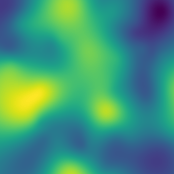
\includegraphics[interpolate=true,width=1.740000in,height=1.740000in]{random_field_regressiom-img0.png}}%
\end{pgfscope}%
\begin{pgfscope}%
\pgfsetbuttcap%
\pgfsetmiterjoin%
\definecolor{currentfill}{rgb}{1.000000,1.000000,1.000000}%
\pgfsetfillcolor{currentfill}%
\pgfsetlinewidth{0.000000pt}%
\definecolor{currentstroke}{rgb}{0.000000,0.000000,0.000000}%
\pgfsetstrokecolor{currentstroke}%
\pgfsetstrokeopacity{0.000000}%
\pgfsetdash{}{0pt}%
\pgfpathmoveto{\pgfqpoint{3.725704in}{0.096475in}}%
\pgfpathlineto{\pgfqpoint{5.462257in}{0.096475in}}%
\pgfpathlineto{\pgfqpoint{5.462257in}{1.833028in}}%
\pgfpathlineto{\pgfqpoint{3.725704in}{1.833028in}}%
\pgfpathlineto{\pgfqpoint{3.725704in}{0.096475in}}%
\pgfpathclose%
\pgfusepath{fill}%
\end{pgfscope}%
\begin{pgfscope}%
\pgfpathrectangle{\pgfqpoint{3.725704in}{0.096475in}}{\pgfqpoint{1.736553in}{1.736553in}}%
\pgfusepath{clip}%
\pgfsys@transformshift{3.725704in}{0.096475in}%
\pgftext[left,bottom]{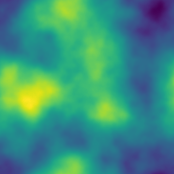
\includegraphics[interpolate=true,width=1.740000in,height=1.740000in]{random_field_regressiom-img1.png}}%
\end{pgfscope}%
\begin{pgfscope}%
\pgfsetbuttcap%
\pgfsetmiterjoin%
\definecolor{currentfill}{rgb}{1.000000,1.000000,1.000000}%
\pgfsetfillcolor{currentfill}%
\pgfsetlinewidth{0.000000pt}%
\definecolor{currentstroke}{rgb}{0.000000,0.000000,0.000000}%
\pgfsetstrokecolor{currentstroke}%
\pgfsetstrokeopacity{0.000000}%
\pgfsetdash{}{0pt}%
\pgfpathmoveto{\pgfqpoint{5.562257in}{0.096475in}}%
\pgfpathlineto{\pgfqpoint{5.735912in}{0.096475in}}%
\pgfpathlineto{\pgfqpoint{5.735912in}{1.833028in}}%
\pgfpathlineto{\pgfqpoint{5.562257in}{1.833028in}}%
\pgfpathlineto{\pgfqpoint{5.562257in}{0.096475in}}%
\pgfpathclose%
\pgfusepath{fill}%
\end{pgfscope}%
\begin{pgfscope}%
\pgfsys@transformshift{5.560000in}{0.109503in}%
\pgftext[left,bottom]{
\includegraphics[interpolate=true,width=0.180000in,height=1.730000in]{random_field_regressiom-img2.png}}%
\end{pgfscope}%
\begin{pgfscope}%
\pgfsetrectcap%
\pgfsetmiterjoin%
\pgfsetlinewidth{0.803000pt}%
\definecolor{currentstroke}{rgb}{0.000000,0.000000,0.000000}%
\pgfsetstrokecolor{currentstroke}%
\pgfsetdash{}{0pt}%
\pgfpathmoveto{\pgfqpoint{5.562257in}{0.096475in}}%
\pgfpathlineto{\pgfqpoint{5.649084in}{0.096475in}}%
\pgfpathlineto{\pgfqpoint{5.735912in}{0.096475in}}%
\pgfpathlineto{\pgfqpoint{5.735912in}{1.833028in}}%
\pgfpathlineto{\pgfqpoint{5.649084in}{1.833028in}}%
\pgfpathlineto{\pgfqpoint{5.562257in}{1.833028in}}%
\pgfpathlineto{\pgfqpoint{5.562257in}{0.096475in}}%
\pgfpathclose%
\pgfusepath{stroke}%
\end{pgfscope}%
\end{pgfpicture}%
\makeatother%
\endgroup%

    \caption{Gaussian random field regression: Sampled points, regression, ground truth and color bar.}
    \label{fig:random_field_regression}
\end{figure}

First we deal with the unbiasedness condition.
We can write the linear predictor as
\[
    \hat{X}_{t} = w^{T} y + c
\]
with \( w = [w_{1}, \dots, w_{n}] \) and \( y = [X_{t_{1}}, \dots, X_{t_{n}}] \).
If we require \( \hat{X_{t}} \) to be unbiased,
\[
    \mu = \E[\hat{X}_{t}] = \E[c + w^{T} y] = c + w^{T} (\mathbf{1}_{n} \mu).
\]
Here we denote by \( \mathbf{1}_{n} \) the vector of length \( n \) with all entries equal to one.
The last equality is due to the observations $y$ being distributed with mean $\mu$.
Thus the constant term must be
\[
    c = \mu - w^{T} (\mathbf{1}_{n} \mu)
\]
and the unbiased predictor is
\[
    \hat{X}_{t} = \mu + w^{T} (y- (\mathbf{1}_{n} \mu)).
\]

Before we deal with the minimization of the mean squared error, we will introduce some notation.
Let us define the vector
\[
    \begin{bmatrix}
    X_{t}\\
    \hat{X}_{M}
    \end{bmatrix},
\]
where $X_{t}$ is the random variable obtained from $X$ at a fixed $t \in T$ and $\hat{X}_{M}$ is the random vector containing measurements \( [X_{t_{1}}, \dots, X_{t_{n}}] \) at points \(M=  \{ t_{1}, \dots, t_{n} \} \subset T \).
This vector is Gaussian with mean 
\[
    \mu = \begin{bmatrix}
    \mu_{t}\\
    \mu_{M}
    \end{bmatrix}
\]
and covariance
\[
    \Sigma = \begin{bmatrix}
    \Sigma_{t,t} & \Sigma_{t, M}\\
    \Sigma_{M, t} & \Sigma_{M,M}
    \end{bmatrix},
\]
where \( \mu_{M} \coloneqq [\mu_{t_{1}}, \dots , \mu_{t_{n}}]^{T} \) 
and the covariance block matrices are given by
\begin{align*}
    \Sigma_{t,t} &= C(t,t)\\
    \Sigma_{t, M} &= [C(t,t_{i})]_{1 \leq i \leq n}\\
    \Sigma_{M, t} &= (\Sigma_{t, M})^{T}\\
    \Sigma_{M,M} &= [C(t_{i},t_{j})]_{1 \leq i,j \leq n}.
\end{align*}
Now we come to the minimization of the mean squared error.
We can reformulate it as 
\begin{align*}
    \operatorname{MSE}(\hat{X}_{t}) &= \E\left[ \left( \hat{X}_{t} - X_{t} \right)^{2} \right]\\
    &= \E\left[ (w^{T}(y-\mu)+(\mu-X_{t}))^2 \right]\\
    &= w^{T} \E[(y-\mu)(y-\mu)^{T}] w + \E[(\mu-X_{t})^2] - 2 \E[w^{T}(y-\mu)(X_{t}-\mu)]\\ 
    &= w^{T} \Sigma_{M, M} w + \Sigma_{t, t} -2 w^{T} \Sigma_{M,t}.
\end{align*}
Differentiating with respect to $w$ and setting the gradient to zero yields
\begin{align*}
    0 &= \frac{\partial}{\partial w} \left( w^{T}\Sigma_{M, M} w + \Sigma_{t, t} -2 w^{T}\Sigma_{M,t} \right) \\
    &= 2\Sigma_{M,M} w - 2 \Sigma_{M,t},
\end{align*}
which is equivalent to
\[
    \Sigma_{M,M} w = \Sigma_{M,t}.
\]
From this we derive the optimal weights \( w = \Sigma_{M,M}^{-1} \Sigma_{M,t} \).
And thus we have the Kriging predictor
\[
    \hat{X}_{t} = \mu + \Sigma_{t,M} \Sigma_{M,M}^{-1} (y-(\mathbf{1}_{n} \mu)),
\]
as well as the resulting mean squared error
\[
    \operatorname{MSE}(\hat{X}_{t}) = \Sigma_{t,t} - \Sigma_{t,M} \Sigma_{M,M}^{-1} \Sigma_{M,t}.
\]

Hence, the Kriging predictor is distributed akin to the conditional distribution of a Gaussian random vector, given the measurements, as described in \cref{lem:conditioned_gaussian_random_vector}.
That is,
\begin{equation}\label{eq:kriging_predictor}
    \hat{X}_{t} \sim \mathcal{N}\left(\mu+\Sigma_{t,M}\Sigma_{M,M}^{-1}(y-(\mathbf{1}_{n}\mu)),\,\, \Sigma_{t,t} - \Sigma_{t,M} \Sigma_{M,M}^{-1} \Sigma_{M,t} \right).
\end{equation}





% Then we know from \cref{lem:conditioned_gaussian_random_vector}, that the conditional distribution of \( X_{t^{*}} \) given \( \hat{X}_{M} \) is
% \[
%     X_{t^{*}} \mid \hat{X}_{M} \sim \mathcal{N}\left(\mu_{t^{*}} + \Sigma_{t^{*}, M} \Sigma_{M,M}^{-1} (\hat{X}_{M} - \mu_{M}),\,\, \Sigma_{t^{*},t^{*}} - \Sigma_{t^{*}, M} \Sigma_{M,M}^{-1} \Sigma_{M,t^{*}}\right).
% \]
As we have seen, Kriging provides the \textit{best linear unbiased predictor} (BLUP)\index{Kriging! BLUP property}.  
It is also an exact interpolator~\cite[p.359]{cressie1993statistics}, meaning that the predictor is exact at the measurement points.
One special property of Gaussian processes is, that the optimal predictor and optimal linear predictor are the same under squared error loss~\cite[p.110]{cressie1993statistics}.
% Without going into further detail, an alternative path to deriving Gaussian process regression is to start with a Bayesian linear regression and utilize a kernel trick as is done in~\cite[p. 156]{shahriari2015taking}.





%%%%%%%%%%%%%%%%%%%%%%%%%%%%%%%%%%%%%%%%%%%%%%%%%%%
%%%%%%%%%%%%%%%%%%%%%%%%%%%%%%%%%%%%%%%%%%%%%%%%%%%
%%% Bayesian Optimization
\section{Bayesian Optimization}~\label{sec:bayes_opt}\index{Bayesian Optimization}
% \begin{figure}[ht]
%     \centering
%     %% Creator: Matplotlib, PGF backend
%%
%% To include the figure in your LaTeX document, write
%%   \input{<filename>.pgf}
%%
%% Make sure the required packages are loaded in your preamble
%%   \usepackage{pgf}
%%
%% Also ensure that all the required font packages are loaded; for instance,
%% the lmodern package is sometimes necessary when using math font.
%%   \usepackage{lmodern}
%%
%% Figures using additional raster images can only be included by \input if
%% they are in the same directory as the main LaTeX file. For loading figures
%% from other directories you can use the `import` package
%%   \usepackage{import}
%%
%% and then include the figures with
%%   \import{<path to file>}{<filename>.pgf}
%%
%% Matplotlib used the following preamble
%%   \def\mathdefault#1{#1}
%%   \everymath=\expandafter{\the\everymath\displaystyle}
%%   \usepackage[T1]{fontenc}
%%   \usepackage{siunitx}
%%   \usepackage{amssymb}
%%   \usepackage{amsmath}
%%   \makeatletter\@ifpackageloaded{underscore}{}{\usepackage[strings]{underscore}}\makeatother
%%
\begingroup%
\makeatletter%
\begin{pgfpicture}%
\pgfpathrectangle{\pgfpointorigin}{\pgfqpoint{5.788510in}{1.929503in}}%
\pgfusepath{use as bounding box, clip}%
\begin{pgfscope}%
\pgfsetbuttcap%
\pgfsetmiterjoin%
\definecolor{currentfill}{rgb}{1.000000,1.000000,1.000000}%
\pgfsetfillcolor{currentfill}%
\pgfsetlinewidth{0.000000pt}%
\definecolor{currentstroke}{rgb}{1.000000,1.000000,1.000000}%
\pgfsetstrokecolor{currentstroke}%
\pgfsetdash{}{0pt}%
\pgfpathmoveto{\pgfqpoint{0.000000in}{0.000000in}}%
\pgfpathlineto{\pgfqpoint{5.788510in}{0.000000in}}%
\pgfpathlineto{\pgfqpoint{5.788510in}{1.929503in}}%
\pgfpathlineto{\pgfqpoint{0.000000in}{1.929503in}}%
\pgfpathlineto{\pgfqpoint{0.000000in}{0.000000in}}%
\pgfpathclose%
\pgfusepath{fill}%
\end{pgfscope}%
\begin{pgfscope}%
\pgfsetbuttcap%
\pgfsetmiterjoin%
\definecolor{currentfill}{rgb}{1.000000,1.000000,1.000000}%
\pgfsetfillcolor{currentfill}%
\pgfsetlinewidth{0.000000pt}%
\definecolor{currentstroke}{rgb}{0.000000,0.000000,0.000000}%
\pgfsetstrokecolor{currentstroke}%
\pgfsetstrokeopacity{0.000000}%
\pgfsetdash{}{0pt}%
\pgfpathmoveto{\pgfqpoint{0.000000in}{0.000000in}}%
\pgfpathlineto{\pgfqpoint{1.862837in}{0.000000in}}%
\pgfpathlineto{\pgfqpoint{1.862837in}{1.543603in}}%
\pgfpathlineto{\pgfqpoint{0.000000in}{1.543603in}}%
\pgfpathlineto{\pgfqpoint{0.000000in}{0.000000in}}%
\pgfpathclose%
\pgfusepath{fill}%
\end{pgfscope}%
\begin{pgfscope}%
\pgfpathrectangle{\pgfqpoint{0.000000in}{0.000000in}}{\pgfqpoint{1.862837in}{1.543603in}}%
\pgfusepath{clip}%
\pgfsetrectcap%
\pgfsetroundjoin%
\pgfsetlinewidth{1.505625pt}%
\definecolor{currentstroke}{rgb}{1.000000,0.745098,0.043137}%
\pgfsetstrokecolor{currentstroke}%
\pgfsetdash{}{0pt}%
\pgfpathmoveto{\pgfqpoint{0.084674in}{0.794601in}}%
\pgfpathlineto{\pgfqpoint{0.088068in}{0.800141in}}%
\pgfpathlineto{\pgfqpoint{0.091462in}{0.843520in}}%
\pgfpathlineto{\pgfqpoint{0.094856in}{0.832327in}}%
\pgfpathlineto{\pgfqpoint{0.098249in}{0.782336in}}%
\pgfpathlineto{\pgfqpoint{0.101643in}{0.838641in}}%
\pgfpathlineto{\pgfqpoint{0.108431in}{0.734274in}}%
\pgfpathlineto{\pgfqpoint{0.115218in}{0.653552in}}%
\pgfpathlineto{\pgfqpoint{0.118612in}{0.586457in}}%
\pgfpathlineto{\pgfqpoint{0.122006in}{0.573435in}}%
\pgfpathlineto{\pgfqpoint{0.128793in}{0.500916in}}%
\pgfpathlineto{\pgfqpoint{0.135581in}{0.622884in}}%
\pgfpathlineto{\pgfqpoint{0.138975in}{0.659603in}}%
\pgfpathlineto{\pgfqpoint{0.142368in}{0.636054in}}%
\pgfpathlineto{\pgfqpoint{0.145762in}{0.575947in}}%
\pgfpathlineto{\pgfqpoint{0.149156in}{0.564020in}}%
\pgfpathlineto{\pgfqpoint{0.152550in}{0.488547in}}%
\pgfpathlineto{\pgfqpoint{0.155943in}{0.479965in}}%
\pgfpathlineto{\pgfqpoint{0.159337in}{0.517646in}}%
\pgfpathlineto{\pgfqpoint{0.162731in}{0.513031in}}%
\pgfpathlineto{\pgfqpoint{0.166125in}{0.621216in}}%
\pgfpathlineto{\pgfqpoint{0.169518in}{0.580526in}}%
\pgfpathlineto{\pgfqpoint{0.172912in}{0.501333in}}%
\pgfpathlineto{\pgfqpoint{0.176306in}{0.523073in}}%
\pgfpathlineto{\pgfqpoint{0.179700in}{0.497368in}}%
\pgfpathlineto{\pgfqpoint{0.183094in}{0.423849in}}%
\pgfpathlineto{\pgfqpoint{0.186487in}{0.514603in}}%
\pgfpathlineto{\pgfqpoint{0.189881in}{0.421164in}}%
\pgfpathlineto{\pgfqpoint{0.193275in}{0.492301in}}%
\pgfpathlineto{\pgfqpoint{0.196669in}{0.499656in}}%
\pgfpathlineto{\pgfqpoint{0.200062in}{0.452382in}}%
\pgfpathlineto{\pgfqpoint{0.203456in}{0.474955in}}%
\pgfpathlineto{\pgfqpoint{0.213637in}{0.594596in}}%
\pgfpathlineto{\pgfqpoint{0.217031in}{0.610689in}}%
\pgfpathlineto{\pgfqpoint{0.223819in}{0.510253in}}%
\pgfpathlineto{\pgfqpoint{0.230606in}{0.738383in}}%
\pgfpathlineto{\pgfqpoint{0.234000in}{0.734122in}}%
\pgfpathlineto{\pgfqpoint{0.237394in}{0.879214in}}%
\pgfpathlineto{\pgfqpoint{0.240788in}{0.875446in}}%
\pgfpathlineto{\pgfqpoint{0.244181in}{0.842498in}}%
\pgfpathlineto{\pgfqpoint{0.247575in}{0.780322in}}%
\pgfpathlineto{\pgfqpoint{0.250969in}{0.670981in}}%
\pgfpathlineto{\pgfqpoint{0.254363in}{0.670008in}}%
\pgfpathlineto{\pgfqpoint{0.257756in}{0.584142in}}%
\pgfpathlineto{\pgfqpoint{0.261150in}{0.562389in}}%
\pgfpathlineto{\pgfqpoint{0.264544in}{0.549206in}}%
\pgfpathlineto{\pgfqpoint{0.267938in}{0.526757in}}%
\pgfpathlineto{\pgfqpoint{0.271331in}{0.491184in}}%
\pgfpathlineto{\pgfqpoint{0.274725in}{0.522678in}}%
\pgfpathlineto{\pgfqpoint{0.278119in}{0.447986in}}%
\pgfpathlineto{\pgfqpoint{0.281513in}{0.470525in}}%
\pgfpathlineto{\pgfqpoint{0.284906in}{0.483481in}}%
\pgfpathlineto{\pgfqpoint{0.288300in}{0.566694in}}%
\pgfpathlineto{\pgfqpoint{0.291694in}{0.575801in}}%
\pgfpathlineto{\pgfqpoint{0.295088in}{0.630565in}}%
\pgfpathlineto{\pgfqpoint{0.298481in}{0.659792in}}%
\pgfpathlineto{\pgfqpoint{0.301875in}{0.718138in}}%
\pgfpathlineto{\pgfqpoint{0.305269in}{0.805648in}}%
\pgfpathlineto{\pgfqpoint{0.308663in}{0.780472in}}%
\pgfpathlineto{\pgfqpoint{0.312057in}{0.770071in}}%
\pgfpathlineto{\pgfqpoint{0.315450in}{0.748643in}}%
\pgfpathlineto{\pgfqpoint{0.318844in}{0.829520in}}%
\pgfpathlineto{\pgfqpoint{0.322238in}{0.877246in}}%
\pgfpathlineto{\pgfqpoint{0.325632in}{0.957295in}}%
\pgfpathlineto{\pgfqpoint{0.329025in}{0.882394in}}%
\pgfpathlineto{\pgfqpoint{0.332419in}{0.908486in}}%
\pgfpathlineto{\pgfqpoint{0.335813in}{0.880731in}}%
\pgfpathlineto{\pgfqpoint{0.339207in}{0.893594in}}%
\pgfpathlineto{\pgfqpoint{0.342600in}{0.925660in}}%
\pgfpathlineto{\pgfqpoint{0.345994in}{0.890903in}}%
\pgfpathlineto{\pgfqpoint{0.352782in}{0.872103in}}%
\pgfpathlineto{\pgfqpoint{0.356175in}{1.041897in}}%
\pgfpathlineto{\pgfqpoint{0.359569in}{1.073514in}}%
\pgfpathlineto{\pgfqpoint{0.362963in}{1.077549in}}%
\pgfpathlineto{\pgfqpoint{0.366357in}{1.060886in}}%
\pgfpathlineto{\pgfqpoint{0.369751in}{0.948955in}}%
\pgfpathlineto{\pgfqpoint{0.373144in}{0.981017in}}%
\pgfpathlineto{\pgfqpoint{0.376538in}{0.981860in}}%
\pgfpathlineto{\pgfqpoint{0.379932in}{0.938528in}}%
\pgfpathlineto{\pgfqpoint{0.383326in}{0.919916in}}%
\pgfpathlineto{\pgfqpoint{0.386719in}{0.797727in}}%
\pgfpathlineto{\pgfqpoint{0.393507in}{0.703608in}}%
\pgfpathlineto{\pgfqpoint{0.396901in}{0.829789in}}%
\pgfpathlineto{\pgfqpoint{0.400294in}{0.869064in}}%
\pgfpathlineto{\pgfqpoint{0.403688in}{0.837591in}}%
\pgfpathlineto{\pgfqpoint{0.407082in}{0.856003in}}%
\pgfpathlineto{\pgfqpoint{0.410476in}{0.742361in}}%
\pgfpathlineto{\pgfqpoint{0.413869in}{0.789394in}}%
\pgfpathlineto{\pgfqpoint{0.424051in}{0.626486in}}%
\pgfpathlineto{\pgfqpoint{0.434232in}{0.819015in}}%
\pgfpathlineto{\pgfqpoint{0.437626in}{0.719856in}}%
\pgfpathlineto{\pgfqpoint{0.441020in}{0.815905in}}%
\pgfpathlineto{\pgfqpoint{0.444413in}{0.823017in}}%
\pgfpathlineto{\pgfqpoint{0.447807in}{0.900181in}}%
\pgfpathlineto{\pgfqpoint{0.451201in}{0.822757in}}%
\pgfpathlineto{\pgfqpoint{0.454595in}{0.907094in}}%
\pgfpathlineto{\pgfqpoint{0.457988in}{0.870803in}}%
\pgfpathlineto{\pgfqpoint{0.461382in}{0.922417in}}%
\pgfpathlineto{\pgfqpoint{0.464776in}{0.915768in}}%
\pgfpathlineto{\pgfqpoint{0.468170in}{0.941156in}}%
\pgfpathlineto{\pgfqpoint{0.471563in}{0.890489in}}%
\pgfpathlineto{\pgfqpoint{0.474957in}{0.938581in}}%
\pgfpathlineto{\pgfqpoint{0.478351in}{0.948544in}}%
\pgfpathlineto{\pgfqpoint{0.481745in}{0.941782in}}%
\pgfpathlineto{\pgfqpoint{0.485138in}{0.940491in}}%
\pgfpathlineto{\pgfqpoint{0.488532in}{1.041011in}}%
\pgfpathlineto{\pgfqpoint{0.491926in}{0.937540in}}%
\pgfpathlineto{\pgfqpoint{0.495320in}{0.955196in}}%
\pgfpathlineto{\pgfqpoint{0.498714in}{0.986336in}}%
\pgfpathlineto{\pgfqpoint{0.502107in}{0.990939in}}%
\pgfpathlineto{\pgfqpoint{0.508895in}{0.928581in}}%
\pgfpathlineto{\pgfqpoint{0.512289in}{1.044449in}}%
\pgfpathlineto{\pgfqpoint{0.519076in}{0.909995in}}%
\pgfpathlineto{\pgfqpoint{0.522470in}{0.914298in}}%
\pgfpathlineto{\pgfqpoint{0.529257in}{0.881311in}}%
\pgfpathlineto{\pgfqpoint{0.532651in}{0.772330in}}%
\pgfpathlineto{\pgfqpoint{0.536045in}{0.745058in}}%
\pgfpathlineto{\pgfqpoint{0.539439in}{0.731497in}}%
\pgfpathlineto{\pgfqpoint{0.542832in}{0.679800in}}%
\pgfpathlineto{\pgfqpoint{0.549620in}{0.538851in}}%
\pgfpathlineto{\pgfqpoint{0.553014in}{0.417893in}}%
\pgfpathlineto{\pgfqpoint{0.559801in}{0.488948in}}%
\pgfpathlineto{\pgfqpoint{0.563195in}{0.481162in}}%
\pgfpathlineto{\pgfqpoint{0.566589in}{0.417272in}}%
\pgfpathlineto{\pgfqpoint{0.569983in}{0.441192in}}%
\pgfpathlineto{\pgfqpoint{0.573376in}{0.406436in}}%
\pgfpathlineto{\pgfqpoint{0.576770in}{0.459620in}}%
\pgfpathlineto{\pgfqpoint{0.580164in}{0.441007in}}%
\pgfpathlineto{\pgfqpoint{0.583558in}{0.268714in}}%
\pgfpathlineto{\pgfqpoint{0.586951in}{0.231825in}}%
\pgfpathlineto{\pgfqpoint{0.590345in}{0.218376in}}%
\pgfpathlineto{\pgfqpoint{0.593739in}{0.261754in}}%
\pgfpathlineto{\pgfqpoint{0.597133in}{0.215782in}}%
\pgfpathlineto{\pgfqpoint{0.603920in}{0.280865in}}%
\pgfpathlineto{\pgfqpoint{0.607314in}{0.268995in}}%
\pgfpathlineto{\pgfqpoint{0.610708in}{0.291653in}}%
\pgfpathlineto{\pgfqpoint{0.614101in}{0.245422in}}%
\pgfpathlineto{\pgfqpoint{0.617495in}{0.376202in}}%
\pgfpathlineto{\pgfqpoint{0.620889in}{0.347949in}}%
\pgfpathlineto{\pgfqpoint{0.624283in}{0.345189in}}%
\pgfpathlineto{\pgfqpoint{0.631070in}{0.531842in}}%
\pgfpathlineto{\pgfqpoint{0.634464in}{0.606281in}}%
\pgfpathlineto{\pgfqpoint{0.637858in}{0.608076in}}%
\pgfpathlineto{\pgfqpoint{0.644645in}{0.537153in}}%
\pgfpathlineto{\pgfqpoint{0.648039in}{0.473644in}}%
\pgfpathlineto{\pgfqpoint{0.651433in}{0.378194in}}%
\pgfpathlineto{\pgfqpoint{0.654827in}{0.385370in}}%
\pgfpathlineto{\pgfqpoint{0.658220in}{0.399761in}}%
\pgfpathlineto{\pgfqpoint{0.661614in}{0.499167in}}%
\pgfpathlineto{\pgfqpoint{0.665008in}{0.557760in}}%
\pgfpathlineto{\pgfqpoint{0.668402in}{0.510117in}}%
\pgfpathlineto{\pgfqpoint{0.671795in}{0.437618in}}%
\pgfpathlineto{\pgfqpoint{0.675189in}{0.394997in}}%
\pgfpathlineto{\pgfqpoint{0.678583in}{0.379174in}}%
\pgfpathlineto{\pgfqpoint{0.681977in}{0.408936in}}%
\pgfpathlineto{\pgfqpoint{0.685370in}{0.339646in}}%
\pgfpathlineto{\pgfqpoint{0.692158in}{0.433938in}}%
\pgfpathlineto{\pgfqpoint{0.695552in}{0.440122in}}%
\pgfpathlineto{\pgfqpoint{0.698946in}{0.457137in}}%
\pgfpathlineto{\pgfqpoint{0.702339in}{0.392158in}}%
\pgfpathlineto{\pgfqpoint{0.705733in}{0.377136in}}%
\pgfpathlineto{\pgfqpoint{0.712521in}{0.261312in}}%
\pgfpathlineto{\pgfqpoint{0.715914in}{0.303187in}}%
\pgfpathlineto{\pgfqpoint{0.719308in}{0.296121in}}%
\pgfpathlineto{\pgfqpoint{0.722702in}{0.417970in}}%
\pgfpathlineto{\pgfqpoint{0.726096in}{0.410152in}}%
\pgfpathlineto{\pgfqpoint{0.729489in}{0.512061in}}%
\pgfpathlineto{\pgfqpoint{0.732883in}{0.499741in}}%
\pgfpathlineto{\pgfqpoint{0.739671in}{0.274851in}}%
\pgfpathlineto{\pgfqpoint{0.743064in}{0.211694in}}%
\pgfpathlineto{\pgfqpoint{0.746458in}{0.201734in}}%
\pgfpathlineto{\pgfqpoint{0.749852in}{0.182799in}}%
\pgfpathlineto{\pgfqpoint{0.753246in}{0.146030in}}%
\pgfpathlineto{\pgfqpoint{0.756640in}{0.144529in}}%
\pgfpathlineto{\pgfqpoint{0.760033in}{0.112254in}}%
\pgfpathlineto{\pgfqpoint{0.766821in}{0.181552in}}%
\pgfpathlineto{\pgfqpoint{0.770215in}{0.293583in}}%
\pgfpathlineto{\pgfqpoint{0.773608in}{0.291707in}}%
\pgfpathlineto{\pgfqpoint{0.777002in}{0.351681in}}%
\pgfpathlineto{\pgfqpoint{0.780396in}{0.384255in}}%
\pgfpathlineto{\pgfqpoint{0.783790in}{0.404062in}}%
\pgfpathlineto{\pgfqpoint{0.787183in}{0.403956in}}%
\pgfpathlineto{\pgfqpoint{0.790577in}{0.470485in}}%
\pgfpathlineto{\pgfqpoint{0.793971in}{0.422794in}}%
\pgfpathlineto{\pgfqpoint{0.797365in}{0.412214in}}%
\pgfpathlineto{\pgfqpoint{0.804152in}{0.498025in}}%
\pgfpathlineto{\pgfqpoint{0.807546in}{0.416758in}}%
\pgfpathlineto{\pgfqpoint{0.810940in}{0.386592in}}%
\pgfpathlineto{\pgfqpoint{0.814334in}{0.400034in}}%
\pgfpathlineto{\pgfqpoint{0.817727in}{0.534187in}}%
\pgfpathlineto{\pgfqpoint{0.821121in}{0.499206in}}%
\pgfpathlineto{\pgfqpoint{0.827909in}{0.570838in}}%
\pgfpathlineto{\pgfqpoint{0.838090in}{0.280138in}}%
\pgfpathlineto{\pgfqpoint{0.841484in}{0.345131in}}%
\pgfpathlineto{\pgfqpoint{0.844877in}{0.338009in}}%
\pgfpathlineto{\pgfqpoint{0.848271in}{0.428982in}}%
\pgfpathlineto{\pgfqpoint{0.851665in}{0.418503in}}%
\pgfpathlineto{\pgfqpoint{0.855059in}{0.441672in}}%
\pgfpathlineto{\pgfqpoint{0.858452in}{0.401483in}}%
\pgfpathlineto{\pgfqpoint{0.861846in}{0.398558in}}%
\pgfpathlineto{\pgfqpoint{0.865240in}{0.456837in}}%
\pgfpathlineto{\pgfqpoint{0.868634in}{0.489040in}}%
\pgfpathlineto{\pgfqpoint{0.872027in}{0.535954in}}%
\pgfpathlineto{\pgfqpoint{0.875421in}{0.534264in}}%
\pgfpathlineto{\pgfqpoint{0.878815in}{0.504860in}}%
\pgfpathlineto{\pgfqpoint{0.882209in}{0.377862in}}%
\pgfpathlineto{\pgfqpoint{0.888996in}{0.397333in}}%
\pgfpathlineto{\pgfqpoint{0.892390in}{0.437727in}}%
\pgfpathlineto{\pgfqpoint{0.895784in}{0.429798in}}%
\pgfpathlineto{\pgfqpoint{0.899178in}{0.429138in}}%
\pgfpathlineto{\pgfqpoint{0.902571in}{0.402263in}}%
\pgfpathlineto{\pgfqpoint{0.905965in}{0.451877in}}%
\pgfpathlineto{\pgfqpoint{0.909359in}{0.483298in}}%
\pgfpathlineto{\pgfqpoint{0.912753in}{0.463268in}}%
\pgfpathlineto{\pgfqpoint{0.916146in}{0.497053in}}%
\pgfpathlineto{\pgfqpoint{0.919540in}{0.483771in}}%
\pgfpathlineto{\pgfqpoint{0.926328in}{0.531193in}}%
\pgfpathlineto{\pgfqpoint{0.929721in}{0.639191in}}%
\pgfpathlineto{\pgfqpoint{0.933115in}{0.654669in}}%
\pgfpathlineto{\pgfqpoint{0.936509in}{0.762931in}}%
\pgfpathlineto{\pgfqpoint{0.939903in}{0.806802in}}%
\pgfpathlineto{\pgfqpoint{0.943297in}{0.923650in}}%
\pgfpathlineto{\pgfqpoint{0.946690in}{0.832904in}}%
\pgfpathlineto{\pgfqpoint{0.950084in}{0.809933in}}%
\pgfpathlineto{\pgfqpoint{0.953478in}{0.755027in}}%
\pgfpathlineto{\pgfqpoint{0.956872in}{0.743059in}}%
\pgfpathlineto{\pgfqpoint{0.960265in}{0.813688in}}%
\pgfpathlineto{\pgfqpoint{0.963659in}{0.856109in}}%
\pgfpathlineto{\pgfqpoint{0.967053in}{0.808293in}}%
\pgfpathlineto{\pgfqpoint{0.970447in}{0.731482in}}%
\pgfpathlineto{\pgfqpoint{0.973840in}{0.740658in}}%
\pgfpathlineto{\pgfqpoint{0.977234in}{0.826618in}}%
\pgfpathlineto{\pgfqpoint{0.980628in}{0.811920in}}%
\pgfpathlineto{\pgfqpoint{0.984022in}{0.815050in}}%
\pgfpathlineto{\pgfqpoint{0.987415in}{0.918094in}}%
\pgfpathlineto{\pgfqpoint{0.997597in}{0.763263in}}%
\pgfpathlineto{\pgfqpoint{1.000990in}{0.749362in}}%
\pgfpathlineto{\pgfqpoint{1.004384in}{0.849175in}}%
\pgfpathlineto{\pgfqpoint{1.007778in}{0.865090in}}%
\pgfpathlineto{\pgfqpoint{1.011172in}{0.896889in}}%
\pgfpathlineto{\pgfqpoint{1.014566in}{0.894491in}}%
\pgfpathlineto{\pgfqpoint{1.017959in}{0.944619in}}%
\pgfpathlineto{\pgfqpoint{1.021353in}{0.961588in}}%
\pgfpathlineto{\pgfqpoint{1.024747in}{0.995147in}}%
\pgfpathlineto{\pgfqpoint{1.028141in}{1.097370in}}%
\pgfpathlineto{\pgfqpoint{1.034928in}{0.980240in}}%
\pgfpathlineto{\pgfqpoint{1.038322in}{0.999775in}}%
\pgfpathlineto{\pgfqpoint{1.041716in}{1.086775in}}%
\pgfpathlineto{\pgfqpoint{1.045109in}{1.127242in}}%
\pgfpathlineto{\pgfqpoint{1.048503in}{1.123273in}}%
\pgfpathlineto{\pgfqpoint{1.051897in}{1.041224in}}%
\pgfpathlineto{\pgfqpoint{1.055291in}{1.060619in}}%
\pgfpathlineto{\pgfqpoint{1.058684in}{1.052431in}}%
\pgfpathlineto{\pgfqpoint{1.062078in}{1.056697in}}%
\pgfpathlineto{\pgfqpoint{1.065472in}{0.988305in}}%
\pgfpathlineto{\pgfqpoint{1.068866in}{1.012744in}}%
\pgfpathlineto{\pgfqpoint{1.072260in}{0.949479in}}%
\pgfpathlineto{\pgfqpoint{1.075653in}{0.986408in}}%
\pgfpathlineto{\pgfqpoint{1.079047in}{0.995747in}}%
\pgfpathlineto{\pgfqpoint{1.082441in}{0.945127in}}%
\pgfpathlineto{\pgfqpoint{1.085835in}{0.921718in}}%
\pgfpathlineto{\pgfqpoint{1.089228in}{0.925037in}}%
\pgfpathlineto{\pgfqpoint{1.092622in}{0.966926in}}%
\pgfpathlineto{\pgfqpoint{1.096016in}{0.966601in}}%
\pgfpathlineto{\pgfqpoint{1.102803in}{0.912672in}}%
\pgfpathlineto{\pgfqpoint{1.106197in}{0.923186in}}%
\pgfpathlineto{\pgfqpoint{1.109591in}{0.967564in}}%
\pgfpathlineto{\pgfqpoint{1.112985in}{0.912731in}}%
\pgfpathlineto{\pgfqpoint{1.116378in}{0.830751in}}%
\pgfpathlineto{\pgfqpoint{1.119772in}{0.894348in}}%
\pgfpathlineto{\pgfqpoint{1.123166in}{0.850159in}}%
\pgfpathlineto{\pgfqpoint{1.126560in}{0.882282in}}%
\pgfpathlineto{\pgfqpoint{1.129953in}{0.943172in}}%
\pgfpathlineto{\pgfqpoint{1.140135in}{1.049953in}}%
\pgfpathlineto{\pgfqpoint{1.143529in}{1.067706in}}%
\pgfpathlineto{\pgfqpoint{1.146922in}{1.146946in}}%
\pgfpathlineto{\pgfqpoint{1.150316in}{1.155618in}}%
\pgfpathlineto{\pgfqpoint{1.153710in}{1.204583in}}%
\pgfpathlineto{\pgfqpoint{1.157104in}{1.107286in}}%
\pgfpathlineto{\pgfqpoint{1.163891in}{1.144038in}}%
\pgfpathlineto{\pgfqpoint{1.167285in}{1.182218in}}%
\pgfpathlineto{\pgfqpoint{1.174072in}{1.139473in}}%
\pgfpathlineto{\pgfqpoint{1.177466in}{1.244435in}}%
\pgfpathlineto{\pgfqpoint{1.180860in}{1.273987in}}%
\pgfpathlineto{\pgfqpoint{1.184254in}{1.265614in}}%
\pgfpathlineto{\pgfqpoint{1.187647in}{1.269794in}}%
\pgfpathlineto{\pgfqpoint{1.191041in}{1.212851in}}%
\pgfpathlineto{\pgfqpoint{1.194435in}{1.200355in}}%
\pgfpathlineto{\pgfqpoint{1.197829in}{1.138304in}}%
\pgfpathlineto{\pgfqpoint{1.201223in}{1.020700in}}%
\pgfpathlineto{\pgfqpoint{1.204616in}{1.036248in}}%
\pgfpathlineto{\pgfqpoint{1.208010in}{1.060197in}}%
\pgfpathlineto{\pgfqpoint{1.211404in}{1.001804in}}%
\pgfpathlineto{\pgfqpoint{1.214798in}{1.010230in}}%
\pgfpathlineto{\pgfqpoint{1.218191in}{0.953972in}}%
\pgfpathlineto{\pgfqpoint{1.221585in}{0.936093in}}%
\pgfpathlineto{\pgfqpoint{1.224979in}{0.927516in}}%
\pgfpathlineto{\pgfqpoint{1.228373in}{0.879520in}}%
\pgfpathlineto{\pgfqpoint{1.231766in}{0.888602in}}%
\pgfpathlineto{\pgfqpoint{1.235160in}{0.861786in}}%
\pgfpathlineto{\pgfqpoint{1.238554in}{0.765742in}}%
\pgfpathlineto{\pgfqpoint{1.241948in}{0.845269in}}%
\pgfpathlineto{\pgfqpoint{1.245341in}{0.891173in}}%
\pgfpathlineto{\pgfqpoint{1.252129in}{0.919360in}}%
\pgfpathlineto{\pgfqpoint{1.255523in}{1.088651in}}%
\pgfpathlineto{\pgfqpoint{1.258916in}{1.060596in}}%
\pgfpathlineto{\pgfqpoint{1.262310in}{1.004946in}}%
\pgfpathlineto{\pgfqpoint{1.265704in}{1.153778in}}%
\pgfpathlineto{\pgfqpoint{1.269098in}{1.156403in}}%
\pgfpathlineto{\pgfqpoint{1.272492in}{1.160727in}}%
\pgfpathlineto{\pgfqpoint{1.275885in}{1.144723in}}%
\pgfpathlineto{\pgfqpoint{1.279279in}{1.216861in}}%
\pgfpathlineto{\pgfqpoint{1.282673in}{1.117989in}}%
\pgfpathlineto{\pgfqpoint{1.286067in}{1.209630in}}%
\pgfpathlineto{\pgfqpoint{1.289460in}{1.223398in}}%
\pgfpathlineto{\pgfqpoint{1.292854in}{1.309128in}}%
\pgfpathlineto{\pgfqpoint{1.296248in}{1.121963in}}%
\pgfpathlineto{\pgfqpoint{1.303035in}{1.115855in}}%
\pgfpathlineto{\pgfqpoint{1.306429in}{1.036648in}}%
\pgfpathlineto{\pgfqpoint{1.309823in}{1.032034in}}%
\pgfpathlineto{\pgfqpoint{1.313217in}{1.071907in}}%
\pgfpathlineto{\pgfqpoint{1.320004in}{1.260962in}}%
\pgfpathlineto{\pgfqpoint{1.323398in}{1.167687in}}%
\pgfpathlineto{\pgfqpoint{1.326792in}{1.213986in}}%
\pgfpathlineto{\pgfqpoint{1.330186in}{1.310606in}}%
\pgfpathlineto{\pgfqpoint{1.333579in}{1.335309in}}%
\pgfpathlineto{\pgfqpoint{1.336973in}{1.304312in}}%
\pgfpathlineto{\pgfqpoint{1.340367in}{1.345923in}}%
\pgfpathlineto{\pgfqpoint{1.343761in}{1.266182in}}%
\pgfpathlineto{\pgfqpoint{1.347154in}{1.253627in}}%
\pgfpathlineto{\pgfqpoint{1.350548in}{1.279891in}}%
\pgfpathlineto{\pgfqpoint{1.353942in}{1.267971in}}%
\pgfpathlineto{\pgfqpoint{1.357336in}{1.251258in}}%
\pgfpathlineto{\pgfqpoint{1.360729in}{1.110731in}}%
\pgfpathlineto{\pgfqpoint{1.364123in}{1.111223in}}%
\pgfpathlineto{\pgfqpoint{1.367517in}{1.012808in}}%
\pgfpathlineto{\pgfqpoint{1.370911in}{0.946784in}}%
\pgfpathlineto{\pgfqpoint{1.374304in}{1.015236in}}%
\pgfpathlineto{\pgfqpoint{1.377698in}{0.986713in}}%
\pgfpathlineto{\pgfqpoint{1.381092in}{0.978660in}}%
\pgfpathlineto{\pgfqpoint{1.384486in}{0.944358in}}%
\pgfpathlineto{\pgfqpoint{1.387879in}{0.829487in}}%
\pgfpathlineto{\pgfqpoint{1.391273in}{0.779146in}}%
\pgfpathlineto{\pgfqpoint{1.394667in}{0.556153in}}%
\pgfpathlineto{\pgfqpoint{1.398061in}{0.679054in}}%
\pgfpathlineto{\pgfqpoint{1.401455in}{0.612905in}}%
\pgfpathlineto{\pgfqpoint{1.404848in}{0.518401in}}%
\pgfpathlineto{\pgfqpoint{1.408242in}{0.500289in}}%
\pgfpathlineto{\pgfqpoint{1.411636in}{0.552903in}}%
\pgfpathlineto{\pgfqpoint{1.415030in}{0.655185in}}%
\pgfpathlineto{\pgfqpoint{1.418423in}{0.633972in}}%
\pgfpathlineto{\pgfqpoint{1.421817in}{0.655238in}}%
\pgfpathlineto{\pgfqpoint{1.425211in}{0.587674in}}%
\pgfpathlineto{\pgfqpoint{1.428605in}{0.567330in}}%
\pgfpathlineto{\pgfqpoint{1.431998in}{0.454111in}}%
\pgfpathlineto{\pgfqpoint{1.435392in}{0.553691in}}%
\pgfpathlineto{\pgfqpoint{1.442180in}{0.602285in}}%
\pgfpathlineto{\pgfqpoint{1.445573in}{0.571148in}}%
\pgfpathlineto{\pgfqpoint{1.448967in}{0.557171in}}%
\pgfpathlineto{\pgfqpoint{1.452361in}{0.605764in}}%
\pgfpathlineto{\pgfqpoint{1.455755in}{0.627018in}}%
\pgfpathlineto{\pgfqpoint{1.459149in}{0.480526in}}%
\pgfpathlineto{\pgfqpoint{1.462542in}{0.564506in}}%
\pgfpathlineto{\pgfqpoint{1.465936in}{0.506406in}}%
\pgfpathlineto{\pgfqpoint{1.469330in}{0.427466in}}%
\pgfpathlineto{\pgfqpoint{1.472724in}{0.460340in}}%
\pgfpathlineto{\pgfqpoint{1.476117in}{0.521534in}}%
\pgfpathlineto{\pgfqpoint{1.479511in}{0.476555in}}%
\pgfpathlineto{\pgfqpoint{1.482905in}{0.449489in}}%
\pgfpathlineto{\pgfqpoint{1.486299in}{0.412670in}}%
\pgfpathlineto{\pgfqpoint{1.489692in}{0.429609in}}%
\pgfpathlineto{\pgfqpoint{1.493086in}{0.429217in}}%
\pgfpathlineto{\pgfqpoint{1.496480in}{0.459698in}}%
\pgfpathlineto{\pgfqpoint{1.499874in}{0.462473in}}%
\pgfpathlineto{\pgfqpoint{1.503267in}{0.494901in}}%
\pgfpathlineto{\pgfqpoint{1.506661in}{0.562246in}}%
\pgfpathlineto{\pgfqpoint{1.510055in}{0.503014in}}%
\pgfpathlineto{\pgfqpoint{1.513449in}{0.474966in}}%
\pgfpathlineto{\pgfqpoint{1.516842in}{0.543716in}}%
\pgfpathlineto{\pgfqpoint{1.520236in}{0.540902in}}%
\pgfpathlineto{\pgfqpoint{1.527024in}{0.685182in}}%
\pgfpathlineto{\pgfqpoint{1.530418in}{0.622268in}}%
\pgfpathlineto{\pgfqpoint{1.533811in}{0.685064in}}%
\pgfpathlineto{\pgfqpoint{1.537205in}{0.674797in}}%
\pgfpathlineto{\pgfqpoint{1.540599in}{0.702869in}}%
\pgfpathlineto{\pgfqpoint{1.543993in}{0.719372in}}%
\pgfpathlineto{\pgfqpoint{1.547386in}{0.658541in}}%
\pgfpathlineto{\pgfqpoint{1.550780in}{0.650738in}}%
\pgfpathlineto{\pgfqpoint{1.554174in}{0.627787in}}%
\pgfpathlineto{\pgfqpoint{1.557568in}{0.628131in}}%
\pgfpathlineto{\pgfqpoint{1.560961in}{0.519515in}}%
\pgfpathlineto{\pgfqpoint{1.564355in}{0.579011in}}%
\pgfpathlineto{\pgfqpoint{1.567749in}{0.560863in}}%
\pgfpathlineto{\pgfqpoint{1.571143in}{0.490441in}}%
\pgfpathlineto{\pgfqpoint{1.574536in}{0.492444in}}%
\pgfpathlineto{\pgfqpoint{1.577930in}{0.447521in}}%
\pgfpathlineto{\pgfqpoint{1.581324in}{0.464513in}}%
\pgfpathlineto{\pgfqpoint{1.584718in}{0.354877in}}%
\pgfpathlineto{\pgfqpoint{1.588112in}{0.337778in}}%
\pgfpathlineto{\pgfqpoint{1.591505in}{0.301495in}}%
\pgfpathlineto{\pgfqpoint{1.594899in}{0.354742in}}%
\pgfpathlineto{\pgfqpoint{1.598293in}{0.324853in}}%
\pgfpathlineto{\pgfqpoint{1.601687in}{0.330543in}}%
\pgfpathlineto{\pgfqpoint{1.605080in}{0.406942in}}%
\pgfpathlineto{\pgfqpoint{1.608474in}{0.435610in}}%
\pgfpathlineto{\pgfqpoint{1.611868in}{0.259522in}}%
\pgfpathlineto{\pgfqpoint{1.615262in}{0.281960in}}%
\pgfpathlineto{\pgfqpoint{1.618655in}{0.357054in}}%
\pgfpathlineto{\pgfqpoint{1.625443in}{0.320921in}}%
\pgfpathlineto{\pgfqpoint{1.628837in}{0.434913in}}%
\pgfpathlineto{\pgfqpoint{1.632230in}{0.400834in}}%
\pgfpathlineto{\pgfqpoint{1.635624in}{0.445401in}}%
\pgfpathlineto{\pgfqpoint{1.639018in}{0.439076in}}%
\pgfpathlineto{\pgfqpoint{1.642412in}{0.334081in}}%
\pgfpathlineto{\pgfqpoint{1.645806in}{0.316220in}}%
\pgfpathlineto{\pgfqpoint{1.649199in}{0.358047in}}%
\pgfpathlineto{\pgfqpoint{1.652593in}{0.370734in}}%
\pgfpathlineto{\pgfqpoint{1.655987in}{0.405639in}}%
\pgfpathlineto{\pgfqpoint{1.659381in}{0.465890in}}%
\pgfpathlineto{\pgfqpoint{1.662774in}{0.437687in}}%
\pgfpathlineto{\pgfqpoint{1.669562in}{0.338376in}}%
\pgfpathlineto{\pgfqpoint{1.672956in}{0.321271in}}%
\pgfpathlineto{\pgfqpoint{1.676349in}{0.379725in}}%
\pgfpathlineto{\pgfqpoint{1.679743in}{0.340935in}}%
\pgfpathlineto{\pgfqpoint{1.683137in}{0.214241in}}%
\pgfpathlineto{\pgfqpoint{1.686531in}{0.192851in}}%
\pgfpathlineto{\pgfqpoint{1.693318in}{0.310462in}}%
\pgfpathlineto{\pgfqpoint{1.696712in}{0.405195in}}%
\pgfpathlineto{\pgfqpoint{1.700106in}{0.387869in}}%
\pgfpathlineto{\pgfqpoint{1.703499in}{0.323909in}}%
\pgfpathlineto{\pgfqpoint{1.706893in}{0.301187in}}%
\pgfpathlineto{\pgfqpoint{1.710287in}{0.290037in}}%
\pgfpathlineto{\pgfqpoint{1.713681in}{0.187063in}}%
\pgfpathlineto{\pgfqpoint{1.717075in}{0.177587in}}%
\pgfpathlineto{\pgfqpoint{1.720468in}{0.162924in}}%
\pgfpathlineto{\pgfqpoint{1.723862in}{0.094133in}}%
\pgfpathlineto{\pgfqpoint{1.727256in}{0.088827in}}%
\pgfpathlineto{\pgfqpoint{1.730650in}{0.135385in}}%
\pgfpathlineto{\pgfqpoint{1.734043in}{0.163753in}}%
\pgfpathlineto{\pgfqpoint{1.737437in}{0.137909in}}%
\pgfpathlineto{\pgfqpoint{1.740831in}{0.209772in}}%
\pgfpathlineto{\pgfqpoint{1.744225in}{0.177943in}}%
\pgfpathlineto{\pgfqpoint{1.747618in}{0.299179in}}%
\pgfpathlineto{\pgfqpoint{1.751012in}{0.281498in}}%
\pgfpathlineto{\pgfqpoint{1.754406in}{0.336095in}}%
\pgfpathlineto{\pgfqpoint{1.757800in}{0.325648in}}%
\pgfpathlineto{\pgfqpoint{1.761193in}{0.311020in}}%
\pgfpathlineto{\pgfqpoint{1.764587in}{0.355586in}}%
\pgfpathlineto{\pgfqpoint{1.767981in}{0.510371in}}%
\pgfpathlineto{\pgfqpoint{1.771375in}{0.461857in}}%
\pgfpathlineto{\pgfqpoint{1.774769in}{0.482427in}}%
\pgfpathlineto{\pgfqpoint{1.778162in}{0.516227in}}%
\pgfpathlineto{\pgfqpoint{1.778162in}{0.516227in}}%
\pgfusepath{stroke}%
\end{pgfscope}%
\begin{pgfscope}%
\pgfpathrectangle{\pgfqpoint{0.000000in}{0.000000in}}{\pgfqpoint{1.862837in}{1.543603in}}%
\pgfusepath{clip}%
\pgfsetrectcap%
\pgfsetroundjoin%
\pgfsetlinewidth{1.505625pt}%
\definecolor{currentstroke}{rgb}{0.984314,0.337255,0.027451}%
\pgfsetstrokecolor{currentstroke}%
\pgfsetdash{}{0pt}%
\pgfpathmoveto{\pgfqpoint{0.084674in}{0.895836in}}%
\pgfpathlineto{\pgfqpoint{0.088068in}{0.850106in}}%
\pgfpathlineto{\pgfqpoint{0.091462in}{0.985234in}}%
\pgfpathlineto{\pgfqpoint{0.098249in}{0.932101in}}%
\pgfpathlineto{\pgfqpoint{0.101643in}{1.009125in}}%
\pgfpathlineto{\pgfqpoint{0.105037in}{1.161879in}}%
\pgfpathlineto{\pgfqpoint{0.108431in}{1.094647in}}%
\pgfpathlineto{\pgfqpoint{0.111825in}{1.090751in}}%
\pgfpathlineto{\pgfqpoint{0.115218in}{1.062492in}}%
\pgfpathlineto{\pgfqpoint{0.118612in}{1.074892in}}%
\pgfpathlineto{\pgfqpoint{0.122006in}{1.158095in}}%
\pgfpathlineto{\pgfqpoint{0.128793in}{1.039811in}}%
\pgfpathlineto{\pgfqpoint{0.132187in}{1.087837in}}%
\pgfpathlineto{\pgfqpoint{0.135581in}{1.030667in}}%
\pgfpathlineto{\pgfqpoint{0.138975in}{1.061594in}}%
\pgfpathlineto{\pgfqpoint{0.142368in}{0.994452in}}%
\pgfpathlineto{\pgfqpoint{0.145762in}{0.978281in}}%
\pgfpathlineto{\pgfqpoint{0.149156in}{1.000278in}}%
\pgfpathlineto{\pgfqpoint{0.152550in}{0.980928in}}%
\pgfpathlineto{\pgfqpoint{0.155943in}{0.918155in}}%
\pgfpathlineto{\pgfqpoint{0.159337in}{0.906993in}}%
\pgfpathlineto{\pgfqpoint{0.162731in}{0.855490in}}%
\pgfpathlineto{\pgfqpoint{0.166125in}{0.837285in}}%
\pgfpathlineto{\pgfqpoint{0.169518in}{0.812044in}}%
\pgfpathlineto{\pgfqpoint{0.172912in}{0.737063in}}%
\pgfpathlineto{\pgfqpoint{0.176306in}{0.789282in}}%
\pgfpathlineto{\pgfqpoint{0.179700in}{0.780081in}}%
\pgfpathlineto{\pgfqpoint{0.183094in}{0.826518in}}%
\pgfpathlineto{\pgfqpoint{0.186487in}{0.796163in}}%
\pgfpathlineto{\pgfqpoint{0.189881in}{0.915821in}}%
\pgfpathlineto{\pgfqpoint{0.193275in}{0.831839in}}%
\pgfpathlineto{\pgfqpoint{0.196669in}{0.784452in}}%
\pgfpathlineto{\pgfqpoint{0.200062in}{0.636625in}}%
\pgfpathlineto{\pgfqpoint{0.203456in}{0.573825in}}%
\pgfpathlineto{\pgfqpoint{0.206850in}{0.638257in}}%
\pgfpathlineto{\pgfqpoint{0.210244in}{0.588974in}}%
\pgfpathlineto{\pgfqpoint{0.213637in}{0.593663in}}%
\pgfpathlineto{\pgfqpoint{0.217031in}{0.552402in}}%
\pgfpathlineto{\pgfqpoint{0.220425in}{0.577821in}}%
\pgfpathlineto{\pgfqpoint{0.223819in}{0.553821in}}%
\pgfpathlineto{\pgfqpoint{0.227212in}{0.671372in}}%
\pgfpathlineto{\pgfqpoint{0.230606in}{0.617350in}}%
\pgfpathlineto{\pgfqpoint{0.234000in}{0.540988in}}%
\pgfpathlineto{\pgfqpoint{0.240788in}{0.546738in}}%
\pgfpathlineto{\pgfqpoint{0.247575in}{0.505781in}}%
\pgfpathlineto{\pgfqpoint{0.250969in}{0.507113in}}%
\pgfpathlineto{\pgfqpoint{0.257756in}{0.440062in}}%
\pgfpathlineto{\pgfqpoint{0.261150in}{0.423803in}}%
\pgfpathlineto{\pgfqpoint{0.264544in}{0.491986in}}%
\pgfpathlineto{\pgfqpoint{0.267938in}{0.535349in}}%
\pgfpathlineto{\pgfqpoint{0.271331in}{0.533909in}}%
\pgfpathlineto{\pgfqpoint{0.274725in}{0.622120in}}%
\pgfpathlineto{\pgfqpoint{0.278119in}{0.619337in}}%
\pgfpathlineto{\pgfqpoint{0.281513in}{0.567322in}}%
\pgfpathlineto{\pgfqpoint{0.284906in}{0.463004in}}%
\pgfpathlineto{\pgfqpoint{0.288300in}{0.401308in}}%
\pgfpathlineto{\pgfqpoint{0.291694in}{0.480336in}}%
\pgfpathlineto{\pgfqpoint{0.295088in}{0.391577in}}%
\pgfpathlineto{\pgfqpoint{0.298481in}{0.426159in}}%
\pgfpathlineto{\pgfqpoint{0.305269in}{0.540093in}}%
\pgfpathlineto{\pgfqpoint{0.308663in}{0.572309in}}%
\pgfpathlineto{\pgfqpoint{0.318844in}{0.762778in}}%
\pgfpathlineto{\pgfqpoint{0.322238in}{0.788926in}}%
\pgfpathlineto{\pgfqpoint{0.325632in}{0.798617in}}%
\pgfpathlineto{\pgfqpoint{0.329025in}{0.800241in}}%
\pgfpathlineto{\pgfqpoint{0.332419in}{0.843824in}}%
\pgfpathlineto{\pgfqpoint{0.335813in}{0.908335in}}%
\pgfpathlineto{\pgfqpoint{0.339207in}{1.002679in}}%
\pgfpathlineto{\pgfqpoint{0.342600in}{1.008913in}}%
\pgfpathlineto{\pgfqpoint{0.345994in}{0.945447in}}%
\pgfpathlineto{\pgfqpoint{0.352782in}{0.901423in}}%
\pgfpathlineto{\pgfqpoint{0.359569in}{0.892210in}}%
\pgfpathlineto{\pgfqpoint{0.362963in}{0.860935in}}%
\pgfpathlineto{\pgfqpoint{0.366357in}{0.747840in}}%
\pgfpathlineto{\pgfqpoint{0.369751in}{0.770018in}}%
\pgfpathlineto{\pgfqpoint{0.373144in}{0.854413in}}%
\pgfpathlineto{\pgfqpoint{0.376538in}{0.885350in}}%
\pgfpathlineto{\pgfqpoint{0.379932in}{0.963304in}}%
\pgfpathlineto{\pgfqpoint{0.383326in}{0.862914in}}%
\pgfpathlineto{\pgfqpoint{0.386719in}{0.863297in}}%
\pgfpathlineto{\pgfqpoint{0.393507in}{1.006381in}}%
\pgfpathlineto{\pgfqpoint{0.396901in}{0.991456in}}%
\pgfpathlineto{\pgfqpoint{0.400294in}{0.968605in}}%
\pgfpathlineto{\pgfqpoint{0.403688in}{1.034616in}}%
\pgfpathlineto{\pgfqpoint{0.407082in}{0.976722in}}%
\pgfpathlineto{\pgfqpoint{0.410476in}{0.983624in}}%
\pgfpathlineto{\pgfqpoint{0.413869in}{0.859366in}}%
\pgfpathlineto{\pgfqpoint{0.417263in}{0.793128in}}%
\pgfpathlineto{\pgfqpoint{0.420657in}{0.791377in}}%
\pgfpathlineto{\pgfqpoint{0.424051in}{0.744507in}}%
\pgfpathlineto{\pgfqpoint{0.427444in}{0.755881in}}%
\pgfpathlineto{\pgfqpoint{0.430838in}{0.692168in}}%
\pgfpathlineto{\pgfqpoint{0.434232in}{0.710023in}}%
\pgfpathlineto{\pgfqpoint{0.437626in}{0.687298in}}%
\pgfpathlineto{\pgfqpoint{0.441020in}{0.602366in}}%
\pgfpathlineto{\pgfqpoint{0.444413in}{0.616018in}}%
\pgfpathlineto{\pgfqpoint{0.447807in}{0.725024in}}%
\pgfpathlineto{\pgfqpoint{0.451201in}{0.764068in}}%
\pgfpathlineto{\pgfqpoint{0.454595in}{0.680288in}}%
\pgfpathlineto{\pgfqpoint{0.457988in}{0.759315in}}%
\pgfpathlineto{\pgfqpoint{0.461382in}{0.802399in}}%
\pgfpathlineto{\pgfqpoint{0.464776in}{0.792124in}}%
\pgfpathlineto{\pgfqpoint{0.468170in}{0.830933in}}%
\pgfpathlineto{\pgfqpoint{0.471563in}{0.690886in}}%
\pgfpathlineto{\pgfqpoint{0.478351in}{0.650379in}}%
\pgfpathlineto{\pgfqpoint{0.481745in}{0.729631in}}%
\pgfpathlineto{\pgfqpoint{0.485138in}{0.731181in}}%
\pgfpathlineto{\pgfqpoint{0.488532in}{0.709936in}}%
\pgfpathlineto{\pgfqpoint{0.491926in}{0.718145in}}%
\pgfpathlineto{\pgfqpoint{0.495320in}{0.702994in}}%
\pgfpathlineto{\pgfqpoint{0.498714in}{0.758780in}}%
\pgfpathlineto{\pgfqpoint{0.502107in}{0.780591in}}%
\pgfpathlineto{\pgfqpoint{0.505501in}{0.776090in}}%
\pgfpathlineto{\pgfqpoint{0.508895in}{0.739702in}}%
\pgfpathlineto{\pgfqpoint{0.512289in}{0.688446in}}%
\pgfpathlineto{\pgfqpoint{0.515682in}{0.720868in}}%
\pgfpathlineto{\pgfqpoint{0.519076in}{0.819128in}}%
\pgfpathlineto{\pgfqpoint{0.522470in}{0.799201in}}%
\pgfpathlineto{\pgfqpoint{0.525864in}{0.798890in}}%
\pgfpathlineto{\pgfqpoint{0.529257in}{0.780569in}}%
\pgfpathlineto{\pgfqpoint{0.532651in}{0.778003in}}%
\pgfpathlineto{\pgfqpoint{0.536045in}{0.899128in}}%
\pgfpathlineto{\pgfqpoint{0.539439in}{0.860876in}}%
\pgfpathlineto{\pgfqpoint{0.542832in}{0.849603in}}%
\pgfpathlineto{\pgfqpoint{0.546226in}{0.854058in}}%
\pgfpathlineto{\pgfqpoint{0.549620in}{0.862851in}}%
\pgfpathlineto{\pgfqpoint{0.553014in}{0.952850in}}%
\pgfpathlineto{\pgfqpoint{0.556407in}{0.985329in}}%
\pgfpathlineto{\pgfqpoint{0.563195in}{0.850871in}}%
\pgfpathlineto{\pgfqpoint{0.566589in}{0.851557in}}%
\pgfpathlineto{\pgfqpoint{0.569983in}{0.874294in}}%
\pgfpathlineto{\pgfqpoint{0.573376in}{0.764568in}}%
\pgfpathlineto{\pgfqpoint{0.576770in}{0.796836in}}%
\pgfpathlineto{\pgfqpoint{0.580164in}{0.690187in}}%
\pgfpathlineto{\pgfqpoint{0.583558in}{0.714734in}}%
\pgfpathlineto{\pgfqpoint{0.586951in}{0.721682in}}%
\pgfpathlineto{\pgfqpoint{0.590345in}{0.767311in}}%
\pgfpathlineto{\pgfqpoint{0.593739in}{0.756377in}}%
\pgfpathlineto{\pgfqpoint{0.597133in}{0.810238in}}%
\pgfpathlineto{\pgfqpoint{0.600526in}{0.832121in}}%
\pgfpathlineto{\pgfqpoint{0.603920in}{0.768074in}}%
\pgfpathlineto{\pgfqpoint{0.617495in}{1.152063in}}%
\pgfpathlineto{\pgfqpoint{0.620889in}{1.203385in}}%
\pgfpathlineto{\pgfqpoint{0.627677in}{1.235155in}}%
\pgfpathlineto{\pgfqpoint{0.631070in}{1.146634in}}%
\pgfpathlineto{\pgfqpoint{0.634464in}{1.137625in}}%
\pgfpathlineto{\pgfqpoint{0.641252in}{1.038186in}}%
\pgfpathlineto{\pgfqpoint{0.644645in}{1.091007in}}%
\pgfpathlineto{\pgfqpoint{0.648039in}{1.082699in}}%
\pgfpathlineto{\pgfqpoint{0.651433in}{1.132263in}}%
\pgfpathlineto{\pgfqpoint{0.658220in}{0.903032in}}%
\pgfpathlineto{\pgfqpoint{0.661614in}{0.865083in}}%
\pgfpathlineto{\pgfqpoint{0.665008in}{0.935967in}}%
\pgfpathlineto{\pgfqpoint{0.668402in}{0.919479in}}%
\pgfpathlineto{\pgfqpoint{0.671795in}{0.938552in}}%
\pgfpathlineto{\pgfqpoint{0.675189in}{0.951206in}}%
\pgfpathlineto{\pgfqpoint{0.678583in}{0.946462in}}%
\pgfpathlineto{\pgfqpoint{0.681977in}{0.923294in}}%
\pgfpathlineto{\pgfqpoint{0.685370in}{0.989110in}}%
\pgfpathlineto{\pgfqpoint{0.688764in}{0.959799in}}%
\pgfpathlineto{\pgfqpoint{0.692158in}{0.995162in}}%
\pgfpathlineto{\pgfqpoint{0.695552in}{1.061214in}}%
\pgfpathlineto{\pgfqpoint{0.702339in}{0.966798in}}%
\pgfpathlineto{\pgfqpoint{0.705733in}{0.933222in}}%
\pgfpathlineto{\pgfqpoint{0.709127in}{0.879764in}}%
\pgfpathlineto{\pgfqpoint{0.712521in}{0.870512in}}%
\pgfpathlineto{\pgfqpoint{0.715914in}{0.870045in}}%
\pgfpathlineto{\pgfqpoint{0.719308in}{0.962657in}}%
\pgfpathlineto{\pgfqpoint{0.722702in}{0.994366in}}%
\pgfpathlineto{\pgfqpoint{0.726096in}{0.950303in}}%
\pgfpathlineto{\pgfqpoint{0.729489in}{0.941553in}}%
\pgfpathlineto{\pgfqpoint{0.732883in}{0.964184in}}%
\pgfpathlineto{\pgfqpoint{0.736277in}{1.036764in}}%
\pgfpathlineto{\pgfqpoint{0.739671in}{1.056638in}}%
\pgfpathlineto{\pgfqpoint{0.746458in}{1.000448in}}%
\pgfpathlineto{\pgfqpoint{0.749852in}{1.003938in}}%
\pgfpathlineto{\pgfqpoint{0.753246in}{0.939433in}}%
\pgfpathlineto{\pgfqpoint{0.756640in}{0.971133in}}%
\pgfpathlineto{\pgfqpoint{0.760033in}{0.959448in}}%
\pgfpathlineto{\pgfqpoint{0.766821in}{1.019183in}}%
\pgfpathlineto{\pgfqpoint{0.773608in}{0.976229in}}%
\pgfpathlineto{\pgfqpoint{0.777002in}{0.892939in}}%
\pgfpathlineto{\pgfqpoint{0.780396in}{0.844866in}}%
\pgfpathlineto{\pgfqpoint{0.783790in}{0.874253in}}%
\pgfpathlineto{\pgfqpoint{0.787183in}{0.975663in}}%
\pgfpathlineto{\pgfqpoint{0.790577in}{1.004579in}}%
\pgfpathlineto{\pgfqpoint{0.793971in}{0.960919in}}%
\pgfpathlineto{\pgfqpoint{0.797365in}{1.015222in}}%
\pgfpathlineto{\pgfqpoint{0.800758in}{0.999809in}}%
\pgfpathlineto{\pgfqpoint{0.804152in}{0.872325in}}%
\pgfpathlineto{\pgfqpoint{0.814334in}{0.914336in}}%
\pgfpathlineto{\pgfqpoint{0.817727in}{0.890317in}}%
\pgfpathlineto{\pgfqpoint{0.821121in}{0.806051in}}%
\pgfpathlineto{\pgfqpoint{0.824515in}{0.805464in}}%
\pgfpathlineto{\pgfqpoint{0.827909in}{0.831932in}}%
\pgfpathlineto{\pgfqpoint{0.831302in}{0.881420in}}%
\pgfpathlineto{\pgfqpoint{0.834696in}{0.965692in}}%
\pgfpathlineto{\pgfqpoint{0.838090in}{1.083500in}}%
\pgfpathlineto{\pgfqpoint{0.841484in}{1.160034in}}%
\pgfpathlineto{\pgfqpoint{0.844877in}{1.113596in}}%
\pgfpathlineto{\pgfqpoint{0.848271in}{1.170921in}}%
\pgfpathlineto{\pgfqpoint{0.851665in}{1.182670in}}%
\pgfpathlineto{\pgfqpoint{0.855059in}{1.162015in}}%
\pgfpathlineto{\pgfqpoint{0.858452in}{1.250748in}}%
\pgfpathlineto{\pgfqpoint{0.861846in}{1.200390in}}%
\pgfpathlineto{\pgfqpoint{0.865240in}{1.234742in}}%
\pgfpathlineto{\pgfqpoint{0.868634in}{1.283946in}}%
\pgfpathlineto{\pgfqpoint{0.875421in}{1.215273in}}%
\pgfpathlineto{\pgfqpoint{0.878815in}{1.293255in}}%
\pgfpathlineto{\pgfqpoint{0.882209in}{1.341213in}}%
\pgfpathlineto{\pgfqpoint{0.885603in}{1.354440in}}%
\pgfpathlineto{\pgfqpoint{0.888996in}{1.197866in}}%
\pgfpathlineto{\pgfqpoint{0.892390in}{1.189050in}}%
\pgfpathlineto{\pgfqpoint{0.895784in}{1.236628in}}%
\pgfpathlineto{\pgfqpoint{0.899178in}{1.202263in}}%
\pgfpathlineto{\pgfqpoint{0.902571in}{1.313218in}}%
\pgfpathlineto{\pgfqpoint{0.905965in}{1.229307in}}%
\pgfpathlineto{\pgfqpoint{0.909359in}{1.204440in}}%
\pgfpathlineto{\pgfqpoint{0.912753in}{1.129321in}}%
\pgfpathlineto{\pgfqpoint{0.916146in}{1.123066in}}%
\pgfpathlineto{\pgfqpoint{0.919540in}{1.203067in}}%
\pgfpathlineto{\pgfqpoint{0.922934in}{1.196120in}}%
\pgfpathlineto{\pgfqpoint{0.926328in}{1.177139in}}%
\pgfpathlineto{\pgfqpoint{0.929721in}{1.106607in}}%
\pgfpathlineto{\pgfqpoint{0.933115in}{1.139746in}}%
\pgfpathlineto{\pgfqpoint{0.936509in}{1.160101in}}%
\pgfpathlineto{\pgfqpoint{0.939903in}{1.092286in}}%
\pgfpathlineto{\pgfqpoint{0.943297in}{1.108007in}}%
\pgfpathlineto{\pgfqpoint{0.946690in}{1.045569in}}%
\pgfpathlineto{\pgfqpoint{0.950084in}{1.049213in}}%
\pgfpathlineto{\pgfqpoint{0.953478in}{1.084029in}}%
\pgfpathlineto{\pgfqpoint{0.956872in}{1.085478in}}%
\pgfpathlineto{\pgfqpoint{0.960265in}{1.183331in}}%
\pgfpathlineto{\pgfqpoint{0.963659in}{1.114489in}}%
\pgfpathlineto{\pgfqpoint{0.967053in}{0.978301in}}%
\pgfpathlineto{\pgfqpoint{0.973840in}{0.902437in}}%
\pgfpathlineto{\pgfqpoint{0.977234in}{0.940000in}}%
\pgfpathlineto{\pgfqpoint{0.980628in}{0.791667in}}%
\pgfpathlineto{\pgfqpoint{0.984022in}{0.856002in}}%
\pgfpathlineto{\pgfqpoint{0.987415in}{0.984450in}}%
\pgfpathlineto{\pgfqpoint{0.990809in}{0.955915in}}%
\pgfpathlineto{\pgfqpoint{0.994203in}{1.039244in}}%
\pgfpathlineto{\pgfqpoint{1.000990in}{0.938649in}}%
\pgfpathlineto{\pgfqpoint{1.004384in}{0.818005in}}%
\pgfpathlineto{\pgfqpoint{1.007778in}{0.640729in}}%
\pgfpathlineto{\pgfqpoint{1.011172in}{0.620063in}}%
\pgfpathlineto{\pgfqpoint{1.014566in}{0.665751in}}%
\pgfpathlineto{\pgfqpoint{1.017959in}{0.634492in}}%
\pgfpathlineto{\pgfqpoint{1.021353in}{0.577286in}}%
\pgfpathlineto{\pgfqpoint{1.028141in}{0.649012in}}%
\pgfpathlineto{\pgfqpoint{1.034928in}{0.807259in}}%
\pgfpathlineto{\pgfqpoint{1.038322in}{0.739240in}}%
\pgfpathlineto{\pgfqpoint{1.041716in}{0.760041in}}%
\pgfpathlineto{\pgfqpoint{1.045109in}{0.695805in}}%
\pgfpathlineto{\pgfqpoint{1.048503in}{0.705248in}}%
\pgfpathlineto{\pgfqpoint{1.051897in}{0.667188in}}%
\pgfpathlineto{\pgfqpoint{1.055291in}{0.680280in}}%
\pgfpathlineto{\pgfqpoint{1.058684in}{0.739917in}}%
\pgfpathlineto{\pgfqpoint{1.062078in}{0.756064in}}%
\pgfpathlineto{\pgfqpoint{1.065472in}{0.738864in}}%
\pgfpathlineto{\pgfqpoint{1.068866in}{0.676210in}}%
\pgfpathlineto{\pgfqpoint{1.072260in}{0.810359in}}%
\pgfpathlineto{\pgfqpoint{1.079047in}{0.832584in}}%
\pgfpathlineto{\pgfqpoint{1.082441in}{0.834721in}}%
\pgfpathlineto{\pgfqpoint{1.085835in}{0.858317in}}%
\pgfpathlineto{\pgfqpoint{1.089228in}{0.913100in}}%
\pgfpathlineto{\pgfqpoint{1.092622in}{0.940391in}}%
\pgfpathlineto{\pgfqpoint{1.096016in}{0.936476in}}%
\pgfpathlineto{\pgfqpoint{1.099410in}{1.043150in}}%
\pgfpathlineto{\pgfqpoint{1.102803in}{1.041220in}}%
\pgfpathlineto{\pgfqpoint{1.106197in}{1.032721in}}%
\pgfpathlineto{\pgfqpoint{1.109591in}{0.993362in}}%
\pgfpathlineto{\pgfqpoint{1.112985in}{0.937983in}}%
\pgfpathlineto{\pgfqpoint{1.116378in}{0.965994in}}%
\pgfpathlineto{\pgfqpoint{1.119772in}{1.028903in}}%
\pgfpathlineto{\pgfqpoint{1.126560in}{0.914390in}}%
\pgfpathlineto{\pgfqpoint{1.129953in}{0.984873in}}%
\pgfpathlineto{\pgfqpoint{1.133347in}{0.921485in}}%
\pgfpathlineto{\pgfqpoint{1.136741in}{0.800182in}}%
\pgfpathlineto{\pgfqpoint{1.140135in}{0.798907in}}%
\pgfpathlineto{\pgfqpoint{1.146922in}{0.755629in}}%
\pgfpathlineto{\pgfqpoint{1.150316in}{0.763900in}}%
\pgfpathlineto{\pgfqpoint{1.153710in}{0.740153in}}%
\pgfpathlineto{\pgfqpoint{1.157104in}{0.728854in}}%
\pgfpathlineto{\pgfqpoint{1.160497in}{0.859592in}}%
\pgfpathlineto{\pgfqpoint{1.177466in}{1.092468in}}%
\pgfpathlineto{\pgfqpoint{1.180860in}{1.096471in}}%
\pgfpathlineto{\pgfqpoint{1.184254in}{1.088916in}}%
\pgfpathlineto{\pgfqpoint{1.187647in}{1.119310in}}%
\pgfpathlineto{\pgfqpoint{1.191041in}{1.249066in}}%
\pgfpathlineto{\pgfqpoint{1.194435in}{1.266756in}}%
\pgfpathlineto{\pgfqpoint{1.197829in}{1.298028in}}%
\pgfpathlineto{\pgfqpoint{1.201223in}{1.282211in}}%
\pgfpathlineto{\pgfqpoint{1.208010in}{1.360822in}}%
\pgfpathlineto{\pgfqpoint{1.211404in}{1.323382in}}%
\pgfpathlineto{\pgfqpoint{1.214798in}{1.393188in}}%
\pgfpathlineto{\pgfqpoint{1.218191in}{1.438431in}}%
\pgfpathlineto{\pgfqpoint{1.224979in}{1.473439in}}%
\pgfpathlineto{\pgfqpoint{1.235160in}{1.248504in}}%
\pgfpathlineto{\pgfqpoint{1.238554in}{1.198949in}}%
\pgfpathlineto{\pgfqpoint{1.241948in}{1.231569in}}%
\pgfpathlineto{\pgfqpoint{1.245341in}{1.111092in}}%
\pgfpathlineto{\pgfqpoint{1.248735in}{1.065087in}}%
\pgfpathlineto{\pgfqpoint{1.255523in}{1.025482in}}%
\pgfpathlineto{\pgfqpoint{1.258916in}{1.061236in}}%
\pgfpathlineto{\pgfqpoint{1.262310in}{1.030476in}}%
\pgfpathlineto{\pgfqpoint{1.265704in}{1.045286in}}%
\pgfpathlineto{\pgfqpoint{1.269098in}{0.868841in}}%
\pgfpathlineto{\pgfqpoint{1.272492in}{0.944981in}}%
\pgfpathlineto{\pgfqpoint{1.275885in}{0.945126in}}%
\pgfpathlineto{\pgfqpoint{1.279279in}{0.965568in}}%
\pgfpathlineto{\pgfqpoint{1.286067in}{0.864484in}}%
\pgfpathlineto{\pgfqpoint{1.289460in}{0.902138in}}%
\pgfpathlineto{\pgfqpoint{1.292854in}{0.923893in}}%
\pgfpathlineto{\pgfqpoint{1.296248in}{0.903582in}}%
\pgfpathlineto{\pgfqpoint{1.299642in}{0.899069in}}%
\pgfpathlineto{\pgfqpoint{1.303035in}{0.879135in}}%
\pgfpathlineto{\pgfqpoint{1.306429in}{0.907435in}}%
\pgfpathlineto{\pgfqpoint{1.309823in}{0.877858in}}%
\pgfpathlineto{\pgfqpoint{1.313217in}{0.914172in}}%
\pgfpathlineto{\pgfqpoint{1.316610in}{0.907518in}}%
\pgfpathlineto{\pgfqpoint{1.320004in}{0.848478in}}%
\pgfpathlineto{\pgfqpoint{1.323398in}{0.904341in}}%
\pgfpathlineto{\pgfqpoint{1.326792in}{0.922716in}}%
\pgfpathlineto{\pgfqpoint{1.330186in}{1.054556in}}%
\pgfpathlineto{\pgfqpoint{1.333579in}{1.042165in}}%
\pgfpathlineto{\pgfqpoint{1.340367in}{0.930549in}}%
\pgfpathlineto{\pgfqpoint{1.343761in}{0.942414in}}%
\pgfpathlineto{\pgfqpoint{1.347154in}{0.968756in}}%
\pgfpathlineto{\pgfqpoint{1.350548in}{0.917141in}}%
\pgfpathlineto{\pgfqpoint{1.353942in}{0.912273in}}%
\pgfpathlineto{\pgfqpoint{1.357336in}{0.846764in}}%
\pgfpathlineto{\pgfqpoint{1.360729in}{0.819629in}}%
\pgfpathlineto{\pgfqpoint{1.364123in}{0.809941in}}%
\pgfpathlineto{\pgfqpoint{1.367517in}{0.825857in}}%
\pgfpathlineto{\pgfqpoint{1.370911in}{0.733352in}}%
\pgfpathlineto{\pgfqpoint{1.374304in}{0.687473in}}%
\pgfpathlineto{\pgfqpoint{1.377698in}{0.736538in}}%
\pgfpathlineto{\pgfqpoint{1.381092in}{0.689587in}}%
\pgfpathlineto{\pgfqpoint{1.384486in}{0.658113in}}%
\pgfpathlineto{\pgfqpoint{1.387879in}{0.654118in}}%
\pgfpathlineto{\pgfqpoint{1.391273in}{0.659341in}}%
\pgfpathlineto{\pgfqpoint{1.394667in}{0.580526in}}%
\pgfpathlineto{\pgfqpoint{1.398061in}{0.580021in}}%
\pgfpathlineto{\pgfqpoint{1.404848in}{0.637453in}}%
\pgfpathlineto{\pgfqpoint{1.408242in}{0.626945in}}%
\pgfpathlineto{\pgfqpoint{1.411636in}{0.625817in}}%
\pgfpathlineto{\pgfqpoint{1.415030in}{0.719171in}}%
\pgfpathlineto{\pgfqpoint{1.418423in}{0.738547in}}%
\pgfpathlineto{\pgfqpoint{1.421817in}{0.777444in}}%
\pgfpathlineto{\pgfqpoint{1.425211in}{0.616420in}}%
\pgfpathlineto{\pgfqpoint{1.428605in}{0.574716in}}%
\pgfpathlineto{\pgfqpoint{1.435392in}{0.406305in}}%
\pgfpathlineto{\pgfqpoint{1.438786in}{0.440664in}}%
\pgfpathlineto{\pgfqpoint{1.442180in}{0.382571in}}%
\pgfpathlineto{\pgfqpoint{1.445573in}{0.389843in}}%
\pgfpathlineto{\pgfqpoint{1.452361in}{0.343917in}}%
\pgfpathlineto{\pgfqpoint{1.455755in}{0.362291in}}%
\pgfpathlineto{\pgfqpoint{1.459149in}{0.297484in}}%
\pgfpathlineto{\pgfqpoint{1.462542in}{0.254957in}}%
\pgfpathlineto{\pgfqpoint{1.465936in}{0.254102in}}%
\pgfpathlineto{\pgfqpoint{1.469330in}{0.279553in}}%
\pgfpathlineto{\pgfqpoint{1.472724in}{0.314278in}}%
\pgfpathlineto{\pgfqpoint{1.482905in}{0.110440in}}%
\pgfpathlineto{\pgfqpoint{1.486299in}{0.175072in}}%
\pgfpathlineto{\pgfqpoint{1.489692in}{0.070164in}}%
\pgfpathlineto{\pgfqpoint{1.493086in}{0.135058in}}%
\pgfpathlineto{\pgfqpoint{1.496480in}{0.090530in}}%
\pgfpathlineto{\pgfqpoint{1.499874in}{0.087436in}}%
\pgfpathlineto{\pgfqpoint{1.503267in}{0.102664in}}%
\pgfpathlineto{\pgfqpoint{1.513449in}{0.336166in}}%
\pgfpathlineto{\pgfqpoint{1.516842in}{0.318725in}}%
\pgfpathlineto{\pgfqpoint{1.520236in}{0.286861in}}%
\pgfpathlineto{\pgfqpoint{1.523630in}{0.390312in}}%
\pgfpathlineto{\pgfqpoint{1.527024in}{0.458909in}}%
\pgfpathlineto{\pgfqpoint{1.530418in}{0.555050in}}%
\pgfpathlineto{\pgfqpoint{1.533811in}{0.507119in}}%
\pgfpathlineto{\pgfqpoint{1.537205in}{0.598359in}}%
\pgfpathlineto{\pgfqpoint{1.540599in}{0.568590in}}%
\pgfpathlineto{\pgfqpoint{1.543993in}{0.562498in}}%
\pgfpathlineto{\pgfqpoint{1.547386in}{0.693672in}}%
\pgfpathlineto{\pgfqpoint{1.550780in}{0.712301in}}%
\pgfpathlineto{\pgfqpoint{1.554174in}{0.701400in}}%
\pgfpathlineto{\pgfqpoint{1.557568in}{0.741238in}}%
\pgfpathlineto{\pgfqpoint{1.560961in}{0.698241in}}%
\pgfpathlineto{\pgfqpoint{1.567749in}{0.850351in}}%
\pgfpathlineto{\pgfqpoint{1.571143in}{0.850427in}}%
\pgfpathlineto{\pgfqpoint{1.574536in}{0.927422in}}%
\pgfpathlineto{\pgfqpoint{1.577930in}{0.955351in}}%
\pgfpathlineto{\pgfqpoint{1.584718in}{1.062187in}}%
\pgfpathlineto{\pgfqpoint{1.588112in}{0.987561in}}%
\pgfpathlineto{\pgfqpoint{1.591505in}{1.093746in}}%
\pgfpathlineto{\pgfqpoint{1.594899in}{1.048486in}}%
\pgfpathlineto{\pgfqpoint{1.598293in}{1.053447in}}%
\pgfpathlineto{\pgfqpoint{1.601687in}{1.028547in}}%
\pgfpathlineto{\pgfqpoint{1.605080in}{0.939517in}}%
\pgfpathlineto{\pgfqpoint{1.608474in}{0.984985in}}%
\pgfpathlineto{\pgfqpoint{1.611868in}{1.006943in}}%
\pgfpathlineto{\pgfqpoint{1.615262in}{0.865186in}}%
\pgfpathlineto{\pgfqpoint{1.618655in}{0.771683in}}%
\pgfpathlineto{\pgfqpoint{1.622049in}{0.770856in}}%
\pgfpathlineto{\pgfqpoint{1.625443in}{0.933159in}}%
\pgfpathlineto{\pgfqpoint{1.628837in}{0.857166in}}%
\pgfpathlineto{\pgfqpoint{1.635624in}{0.964870in}}%
\pgfpathlineto{\pgfqpoint{1.639018in}{0.939239in}}%
\pgfpathlineto{\pgfqpoint{1.642412in}{0.940391in}}%
\pgfpathlineto{\pgfqpoint{1.645806in}{1.067857in}}%
\pgfpathlineto{\pgfqpoint{1.649199in}{1.110209in}}%
\pgfpathlineto{\pgfqpoint{1.652593in}{0.995134in}}%
\pgfpathlineto{\pgfqpoint{1.655987in}{0.933414in}}%
\pgfpathlineto{\pgfqpoint{1.659381in}{0.952983in}}%
\pgfpathlineto{\pgfqpoint{1.662774in}{0.951835in}}%
\pgfpathlineto{\pgfqpoint{1.666168in}{0.971574in}}%
\pgfpathlineto{\pgfqpoint{1.669562in}{0.973521in}}%
\pgfpathlineto{\pgfqpoint{1.672956in}{0.933126in}}%
\pgfpathlineto{\pgfqpoint{1.676349in}{0.968712in}}%
\pgfpathlineto{\pgfqpoint{1.679743in}{1.045548in}}%
\pgfpathlineto{\pgfqpoint{1.683137in}{1.095982in}}%
\pgfpathlineto{\pgfqpoint{1.689924in}{1.126288in}}%
\pgfpathlineto{\pgfqpoint{1.693318in}{1.212105in}}%
\pgfpathlineto{\pgfqpoint{1.700106in}{1.156032in}}%
\pgfpathlineto{\pgfqpoint{1.706893in}{1.264153in}}%
\pgfpathlineto{\pgfqpoint{1.710287in}{1.350526in}}%
\pgfpathlineto{\pgfqpoint{1.713681in}{1.268598in}}%
\pgfpathlineto{\pgfqpoint{1.717075in}{1.247895in}}%
\pgfpathlineto{\pgfqpoint{1.720468in}{1.181377in}}%
\pgfpathlineto{\pgfqpoint{1.723862in}{1.194942in}}%
\pgfpathlineto{\pgfqpoint{1.727256in}{1.150314in}}%
\pgfpathlineto{\pgfqpoint{1.730650in}{1.123078in}}%
\pgfpathlineto{\pgfqpoint{1.734043in}{1.024018in}}%
\pgfpathlineto{\pgfqpoint{1.737437in}{1.024714in}}%
\pgfpathlineto{\pgfqpoint{1.740831in}{1.002981in}}%
\pgfpathlineto{\pgfqpoint{1.744225in}{1.031268in}}%
\pgfpathlineto{\pgfqpoint{1.747618in}{0.986949in}}%
\pgfpathlineto{\pgfqpoint{1.751012in}{1.022079in}}%
\pgfpathlineto{\pgfqpoint{1.754406in}{1.009965in}}%
\pgfpathlineto{\pgfqpoint{1.757800in}{0.950143in}}%
\pgfpathlineto{\pgfqpoint{1.761193in}{1.063106in}}%
\pgfpathlineto{\pgfqpoint{1.764587in}{1.024961in}}%
\pgfpathlineto{\pgfqpoint{1.767981in}{1.060631in}}%
\pgfpathlineto{\pgfqpoint{1.771375in}{0.980750in}}%
\pgfpathlineto{\pgfqpoint{1.778162in}{0.859024in}}%
\pgfpathlineto{\pgfqpoint{1.778162in}{0.859024in}}%
\pgfusepath{stroke}%
\end{pgfscope}%
\begin{pgfscope}%
\pgfpathrectangle{\pgfqpoint{0.000000in}{0.000000in}}{\pgfqpoint{1.862837in}{1.543603in}}%
\pgfusepath{clip}%
\pgfsetrectcap%
\pgfsetroundjoin%
\pgfsetlinewidth{1.505625pt}%
\definecolor{currentstroke}{rgb}{1.000000,0.000000,0.431373}%
\pgfsetstrokecolor{currentstroke}%
\pgfsetdash{}{0pt}%
\pgfpathmoveto{\pgfqpoint{0.084674in}{1.018501in}}%
\pgfpathlineto{\pgfqpoint{0.088068in}{1.018695in}}%
\pgfpathlineto{\pgfqpoint{0.091462in}{0.966860in}}%
\pgfpathlineto{\pgfqpoint{0.098249in}{0.896382in}}%
\pgfpathlineto{\pgfqpoint{0.101643in}{0.829518in}}%
\pgfpathlineto{\pgfqpoint{0.105037in}{0.924725in}}%
\pgfpathlineto{\pgfqpoint{0.108431in}{0.895018in}}%
\pgfpathlineto{\pgfqpoint{0.111825in}{0.881326in}}%
\pgfpathlineto{\pgfqpoint{0.118612in}{0.959196in}}%
\pgfpathlineto{\pgfqpoint{0.122006in}{0.973480in}}%
\pgfpathlineto{\pgfqpoint{0.128793in}{0.816761in}}%
\pgfpathlineto{\pgfqpoint{0.132187in}{0.703206in}}%
\pgfpathlineto{\pgfqpoint{0.135581in}{0.676144in}}%
\pgfpathlineto{\pgfqpoint{0.138975in}{0.617565in}}%
\pgfpathlineto{\pgfqpoint{0.142368in}{0.756018in}}%
\pgfpathlineto{\pgfqpoint{0.145762in}{0.722314in}}%
\pgfpathlineto{\pgfqpoint{0.149156in}{0.535769in}}%
\pgfpathlineto{\pgfqpoint{0.152550in}{0.523413in}}%
\pgfpathlineto{\pgfqpoint{0.155943in}{0.548442in}}%
\pgfpathlineto{\pgfqpoint{0.159337in}{0.510909in}}%
\pgfpathlineto{\pgfqpoint{0.162731in}{0.505130in}}%
\pgfpathlineto{\pgfqpoint{0.166125in}{0.433401in}}%
\pgfpathlineto{\pgfqpoint{0.172912in}{0.641884in}}%
\pgfpathlineto{\pgfqpoint{0.176306in}{0.662892in}}%
\pgfpathlineto{\pgfqpoint{0.179700in}{0.703636in}}%
\pgfpathlineto{\pgfqpoint{0.183094in}{0.762877in}}%
\pgfpathlineto{\pgfqpoint{0.186487in}{0.767348in}}%
\pgfpathlineto{\pgfqpoint{0.189881in}{0.688703in}}%
\pgfpathlineto{\pgfqpoint{0.193275in}{0.719347in}}%
\pgfpathlineto{\pgfqpoint{0.196669in}{0.808854in}}%
\pgfpathlineto{\pgfqpoint{0.206850in}{0.860876in}}%
\pgfpathlineto{\pgfqpoint{0.210244in}{0.840949in}}%
\pgfpathlineto{\pgfqpoint{0.213637in}{0.762667in}}%
\pgfpathlineto{\pgfqpoint{0.217031in}{0.791286in}}%
\pgfpathlineto{\pgfqpoint{0.220425in}{0.799213in}}%
\pgfpathlineto{\pgfqpoint{0.223819in}{0.955795in}}%
\pgfpathlineto{\pgfqpoint{0.227212in}{0.920965in}}%
\pgfpathlineto{\pgfqpoint{0.234000in}{0.811653in}}%
\pgfpathlineto{\pgfqpoint{0.237394in}{0.714313in}}%
\pgfpathlineto{\pgfqpoint{0.240788in}{0.816415in}}%
\pgfpathlineto{\pgfqpoint{0.244181in}{0.756409in}}%
\pgfpathlineto{\pgfqpoint{0.247575in}{0.727196in}}%
\pgfpathlineto{\pgfqpoint{0.250969in}{0.791687in}}%
\pgfpathlineto{\pgfqpoint{0.254363in}{0.787730in}}%
\pgfpathlineto{\pgfqpoint{0.257756in}{0.835938in}}%
\pgfpathlineto{\pgfqpoint{0.261150in}{0.843289in}}%
\pgfpathlineto{\pgfqpoint{0.264544in}{0.828289in}}%
\pgfpathlineto{\pgfqpoint{0.267938in}{0.739139in}}%
\pgfpathlineto{\pgfqpoint{0.274725in}{0.773828in}}%
\pgfpathlineto{\pgfqpoint{0.278119in}{0.865738in}}%
\pgfpathlineto{\pgfqpoint{0.281513in}{0.839048in}}%
\pgfpathlineto{\pgfqpoint{0.284906in}{0.791569in}}%
\pgfpathlineto{\pgfqpoint{0.288300in}{0.926421in}}%
\pgfpathlineto{\pgfqpoint{0.301875in}{0.768072in}}%
\pgfpathlineto{\pgfqpoint{0.305269in}{0.863218in}}%
\pgfpathlineto{\pgfqpoint{0.308663in}{0.863299in}}%
\pgfpathlineto{\pgfqpoint{0.312057in}{0.948205in}}%
\pgfpathlineto{\pgfqpoint{0.315450in}{0.931477in}}%
\pgfpathlineto{\pgfqpoint{0.318844in}{0.938756in}}%
\pgfpathlineto{\pgfqpoint{0.322238in}{0.969715in}}%
\pgfpathlineto{\pgfqpoint{0.325632in}{0.902047in}}%
\pgfpathlineto{\pgfqpoint{0.329025in}{0.960623in}}%
\pgfpathlineto{\pgfqpoint{0.332419in}{0.879074in}}%
\pgfpathlineto{\pgfqpoint{0.335813in}{0.840305in}}%
\pgfpathlineto{\pgfqpoint{0.339207in}{0.779595in}}%
\pgfpathlineto{\pgfqpoint{0.342600in}{0.778669in}}%
\pgfpathlineto{\pgfqpoint{0.345994in}{0.876620in}}%
\pgfpathlineto{\pgfqpoint{0.349388in}{0.864969in}}%
\pgfpathlineto{\pgfqpoint{0.352782in}{0.913409in}}%
\pgfpathlineto{\pgfqpoint{0.356175in}{1.011070in}}%
\pgfpathlineto{\pgfqpoint{0.359569in}{0.984155in}}%
\pgfpathlineto{\pgfqpoint{0.362963in}{0.983054in}}%
\pgfpathlineto{\pgfqpoint{0.366357in}{1.011320in}}%
\pgfpathlineto{\pgfqpoint{0.369751in}{0.959541in}}%
\pgfpathlineto{\pgfqpoint{0.373144in}{0.934872in}}%
\pgfpathlineto{\pgfqpoint{0.379932in}{1.076339in}}%
\pgfpathlineto{\pgfqpoint{0.383326in}{0.975707in}}%
\pgfpathlineto{\pgfqpoint{0.386719in}{0.960970in}}%
\pgfpathlineto{\pgfqpoint{0.390113in}{0.875360in}}%
\pgfpathlineto{\pgfqpoint{0.393507in}{0.945969in}}%
\pgfpathlineto{\pgfqpoint{0.396901in}{0.961404in}}%
\pgfpathlineto{\pgfqpoint{0.400294in}{0.922395in}}%
\pgfpathlineto{\pgfqpoint{0.403688in}{0.972571in}}%
\pgfpathlineto{\pgfqpoint{0.407082in}{0.970441in}}%
\pgfpathlineto{\pgfqpoint{0.410476in}{1.065824in}}%
\pgfpathlineto{\pgfqpoint{0.413869in}{1.019037in}}%
\pgfpathlineto{\pgfqpoint{0.417263in}{0.931626in}}%
\pgfpathlineto{\pgfqpoint{0.420657in}{0.912763in}}%
\pgfpathlineto{\pgfqpoint{0.424051in}{0.826241in}}%
\pgfpathlineto{\pgfqpoint{0.427444in}{0.845903in}}%
\pgfpathlineto{\pgfqpoint{0.430838in}{0.875464in}}%
\pgfpathlineto{\pgfqpoint{0.434232in}{0.883732in}}%
\pgfpathlineto{\pgfqpoint{0.437626in}{0.939762in}}%
\pgfpathlineto{\pgfqpoint{0.441020in}{0.931650in}}%
\pgfpathlineto{\pgfqpoint{0.444413in}{1.048057in}}%
\pgfpathlineto{\pgfqpoint{0.447807in}{1.011024in}}%
\pgfpathlineto{\pgfqpoint{0.454595in}{1.053617in}}%
\pgfpathlineto{\pgfqpoint{0.457988in}{1.005773in}}%
\pgfpathlineto{\pgfqpoint{0.461382in}{1.048368in}}%
\pgfpathlineto{\pgfqpoint{0.464776in}{0.993483in}}%
\pgfpathlineto{\pgfqpoint{0.468170in}{1.039261in}}%
\pgfpathlineto{\pgfqpoint{0.471563in}{1.066212in}}%
\pgfpathlineto{\pgfqpoint{0.474957in}{1.082003in}}%
\pgfpathlineto{\pgfqpoint{0.478351in}{1.082385in}}%
\pgfpathlineto{\pgfqpoint{0.481745in}{1.020934in}}%
\pgfpathlineto{\pgfqpoint{0.485138in}{1.021437in}}%
\pgfpathlineto{\pgfqpoint{0.488532in}{0.929726in}}%
\pgfpathlineto{\pgfqpoint{0.491926in}{0.929523in}}%
\pgfpathlineto{\pgfqpoint{0.495320in}{0.921337in}}%
\pgfpathlineto{\pgfqpoint{0.498714in}{0.963683in}}%
\pgfpathlineto{\pgfqpoint{0.502107in}{0.919516in}}%
\pgfpathlineto{\pgfqpoint{0.505501in}{0.845591in}}%
\pgfpathlineto{\pgfqpoint{0.508895in}{0.796396in}}%
\pgfpathlineto{\pgfqpoint{0.512289in}{0.793858in}}%
\pgfpathlineto{\pgfqpoint{0.515682in}{0.688459in}}%
\pgfpathlineto{\pgfqpoint{0.519076in}{0.636473in}}%
\pgfpathlineto{\pgfqpoint{0.522470in}{0.603009in}}%
\pgfpathlineto{\pgfqpoint{0.525864in}{0.539249in}}%
\pgfpathlineto{\pgfqpoint{0.529257in}{0.571190in}}%
\pgfpathlineto{\pgfqpoint{0.532651in}{0.591160in}}%
\pgfpathlineto{\pgfqpoint{0.536045in}{0.622834in}}%
\pgfpathlineto{\pgfqpoint{0.539439in}{0.543288in}}%
\pgfpathlineto{\pgfqpoint{0.546226in}{0.525086in}}%
\pgfpathlineto{\pgfqpoint{0.549620in}{0.575947in}}%
\pgfpathlineto{\pgfqpoint{0.553014in}{0.522671in}}%
\pgfpathlineto{\pgfqpoint{0.556407in}{0.536505in}}%
\pgfpathlineto{\pgfqpoint{0.559801in}{0.470912in}}%
\pgfpathlineto{\pgfqpoint{0.563195in}{0.329101in}}%
\pgfpathlineto{\pgfqpoint{0.566589in}{0.350712in}}%
\pgfpathlineto{\pgfqpoint{0.569983in}{0.384581in}}%
\pgfpathlineto{\pgfqpoint{0.576770in}{0.192003in}}%
\pgfpathlineto{\pgfqpoint{0.580164in}{0.238470in}}%
\pgfpathlineto{\pgfqpoint{0.583558in}{0.224230in}}%
\pgfpathlineto{\pgfqpoint{0.586951in}{0.227327in}}%
\pgfpathlineto{\pgfqpoint{0.590345in}{0.260031in}}%
\pgfpathlineto{\pgfqpoint{0.593739in}{0.152156in}}%
\pgfpathlineto{\pgfqpoint{0.597133in}{0.206470in}}%
\pgfpathlineto{\pgfqpoint{0.600526in}{0.095096in}}%
\pgfpathlineto{\pgfqpoint{0.603920in}{0.121643in}}%
\pgfpathlineto{\pgfqpoint{0.607314in}{0.210941in}}%
\pgfpathlineto{\pgfqpoint{0.610708in}{0.385796in}}%
\pgfpathlineto{\pgfqpoint{0.614101in}{0.337300in}}%
\pgfpathlineto{\pgfqpoint{0.617495in}{0.461571in}}%
\pgfpathlineto{\pgfqpoint{0.620889in}{0.493355in}}%
\pgfpathlineto{\pgfqpoint{0.624283in}{0.537221in}}%
\pgfpathlineto{\pgfqpoint{0.627677in}{0.521922in}}%
\pgfpathlineto{\pgfqpoint{0.631070in}{0.487539in}}%
\pgfpathlineto{\pgfqpoint{0.634464in}{0.487009in}}%
\pgfpathlineto{\pgfqpoint{0.637858in}{0.538940in}}%
\pgfpathlineto{\pgfqpoint{0.641252in}{0.566427in}}%
\pgfpathlineto{\pgfqpoint{0.644645in}{0.617656in}}%
\pgfpathlineto{\pgfqpoint{0.648039in}{0.691935in}}%
\pgfpathlineto{\pgfqpoint{0.651433in}{0.619660in}}%
\pgfpathlineto{\pgfqpoint{0.658220in}{0.780089in}}%
\pgfpathlineto{\pgfqpoint{0.661614in}{0.780846in}}%
\pgfpathlineto{\pgfqpoint{0.665008in}{0.760907in}}%
\pgfpathlineto{\pgfqpoint{0.668402in}{0.767389in}}%
\pgfpathlineto{\pgfqpoint{0.671795in}{0.881067in}}%
\pgfpathlineto{\pgfqpoint{0.675189in}{0.853303in}}%
\pgfpathlineto{\pgfqpoint{0.678583in}{0.806435in}}%
\pgfpathlineto{\pgfqpoint{0.681977in}{0.840342in}}%
\pgfpathlineto{\pgfqpoint{0.688764in}{0.718291in}}%
\pgfpathlineto{\pgfqpoint{0.692158in}{0.715625in}}%
\pgfpathlineto{\pgfqpoint{0.695552in}{0.845032in}}%
\pgfpathlineto{\pgfqpoint{0.698946in}{0.833485in}}%
\pgfpathlineto{\pgfqpoint{0.702339in}{0.891778in}}%
\pgfpathlineto{\pgfqpoint{0.705733in}{0.812979in}}%
\pgfpathlineto{\pgfqpoint{0.709127in}{0.760416in}}%
\pgfpathlineto{\pgfqpoint{0.712521in}{0.784515in}}%
\pgfpathlineto{\pgfqpoint{0.715914in}{0.703926in}}%
\pgfpathlineto{\pgfqpoint{0.726096in}{0.912272in}}%
\pgfpathlineto{\pgfqpoint{0.729489in}{0.997653in}}%
\pgfpathlineto{\pgfqpoint{0.732883in}{1.003440in}}%
\pgfpathlineto{\pgfqpoint{0.739671in}{1.018851in}}%
\pgfpathlineto{\pgfqpoint{0.743064in}{1.102361in}}%
\pgfpathlineto{\pgfqpoint{0.746458in}{1.035290in}}%
\pgfpathlineto{\pgfqpoint{0.749852in}{1.051707in}}%
\pgfpathlineto{\pgfqpoint{0.753246in}{1.017380in}}%
\pgfpathlineto{\pgfqpoint{0.756640in}{1.001423in}}%
\pgfpathlineto{\pgfqpoint{0.760033in}{1.020264in}}%
\pgfpathlineto{\pgfqpoint{0.763427in}{1.007415in}}%
\pgfpathlineto{\pgfqpoint{0.766821in}{0.986127in}}%
\pgfpathlineto{\pgfqpoint{0.770215in}{0.949764in}}%
\pgfpathlineto{\pgfqpoint{0.773608in}{0.886366in}}%
\pgfpathlineto{\pgfqpoint{0.777002in}{0.855592in}}%
\pgfpathlineto{\pgfqpoint{0.780396in}{0.939629in}}%
\pgfpathlineto{\pgfqpoint{0.783790in}{0.896107in}}%
\pgfpathlineto{\pgfqpoint{0.787183in}{0.929277in}}%
\pgfpathlineto{\pgfqpoint{0.790577in}{0.942788in}}%
\pgfpathlineto{\pgfqpoint{0.793971in}{1.064820in}}%
\pgfpathlineto{\pgfqpoint{0.797365in}{1.079473in}}%
\pgfpathlineto{\pgfqpoint{0.804152in}{0.993779in}}%
\pgfpathlineto{\pgfqpoint{0.807546in}{0.991158in}}%
\pgfpathlineto{\pgfqpoint{0.810940in}{0.969176in}}%
\pgfpathlineto{\pgfqpoint{0.821121in}{0.794600in}}%
\pgfpathlineto{\pgfqpoint{0.824515in}{0.679062in}}%
\pgfpathlineto{\pgfqpoint{0.827909in}{0.604860in}}%
\pgfpathlineto{\pgfqpoint{0.831302in}{0.584284in}}%
\pgfpathlineto{\pgfqpoint{0.834696in}{0.578718in}}%
\pgfpathlineto{\pgfqpoint{0.841484in}{0.550301in}}%
\pgfpathlineto{\pgfqpoint{0.844877in}{0.590164in}}%
\pgfpathlineto{\pgfqpoint{0.848271in}{0.610776in}}%
\pgfpathlineto{\pgfqpoint{0.851665in}{0.655828in}}%
\pgfpathlineto{\pgfqpoint{0.855059in}{0.726257in}}%
\pgfpathlineto{\pgfqpoint{0.858452in}{0.668956in}}%
\pgfpathlineto{\pgfqpoint{0.865240in}{0.688598in}}%
\pgfpathlineto{\pgfqpoint{0.868634in}{0.734884in}}%
\pgfpathlineto{\pgfqpoint{0.872027in}{0.689198in}}%
\pgfpathlineto{\pgfqpoint{0.875421in}{0.741075in}}%
\pgfpathlineto{\pgfqpoint{0.882209in}{0.749142in}}%
\pgfpathlineto{\pgfqpoint{0.885603in}{0.720440in}}%
\pgfpathlineto{\pgfqpoint{0.888996in}{0.746635in}}%
\pgfpathlineto{\pgfqpoint{0.895784in}{0.693957in}}%
\pgfpathlineto{\pgfqpoint{0.899178in}{0.776997in}}%
\pgfpathlineto{\pgfqpoint{0.905965in}{0.741816in}}%
\pgfpathlineto{\pgfqpoint{0.909359in}{0.886898in}}%
\pgfpathlineto{\pgfqpoint{0.912753in}{0.867949in}}%
\pgfpathlineto{\pgfqpoint{0.916146in}{0.859885in}}%
\pgfpathlineto{\pgfqpoint{0.919540in}{0.827626in}}%
\pgfpathlineto{\pgfqpoint{0.922934in}{0.850742in}}%
\pgfpathlineto{\pgfqpoint{0.926328in}{0.835219in}}%
\pgfpathlineto{\pgfqpoint{0.929721in}{0.793299in}}%
\pgfpathlineto{\pgfqpoint{0.933115in}{0.870820in}}%
\pgfpathlineto{\pgfqpoint{0.936509in}{0.840239in}}%
\pgfpathlineto{\pgfqpoint{0.939903in}{0.845518in}}%
\pgfpathlineto{\pgfqpoint{0.943297in}{0.807118in}}%
\pgfpathlineto{\pgfqpoint{0.946690in}{0.808102in}}%
\pgfpathlineto{\pgfqpoint{0.950084in}{0.839877in}}%
\pgfpathlineto{\pgfqpoint{0.953478in}{0.750237in}}%
\pgfpathlineto{\pgfqpoint{0.956872in}{0.731145in}}%
\pgfpathlineto{\pgfqpoint{0.960265in}{0.759737in}}%
\pgfpathlineto{\pgfqpoint{0.963659in}{0.770998in}}%
\pgfpathlineto{\pgfqpoint{0.967053in}{0.815712in}}%
\pgfpathlineto{\pgfqpoint{0.970447in}{0.825513in}}%
\pgfpathlineto{\pgfqpoint{0.973840in}{0.822392in}}%
\pgfpathlineto{\pgfqpoint{0.977234in}{0.937354in}}%
\pgfpathlineto{\pgfqpoint{0.980628in}{0.936736in}}%
\pgfpathlineto{\pgfqpoint{0.984022in}{0.890328in}}%
\pgfpathlineto{\pgfqpoint{0.987415in}{0.863647in}}%
\pgfpathlineto{\pgfqpoint{0.990809in}{0.854253in}}%
\pgfpathlineto{\pgfqpoint{0.994203in}{0.879924in}}%
\pgfpathlineto{\pgfqpoint{0.997597in}{0.800281in}}%
\pgfpathlineto{\pgfqpoint{1.000990in}{0.799598in}}%
\pgfpathlineto{\pgfqpoint{1.004384in}{0.693257in}}%
\pgfpathlineto{\pgfqpoint{1.007778in}{0.739834in}}%
\pgfpathlineto{\pgfqpoint{1.011172in}{0.677377in}}%
\pgfpathlineto{\pgfqpoint{1.014566in}{0.760010in}}%
\pgfpathlineto{\pgfqpoint{1.017959in}{0.717042in}}%
\pgfpathlineto{\pgfqpoint{1.021353in}{0.704341in}}%
\pgfpathlineto{\pgfqpoint{1.024747in}{0.643777in}}%
\pgfpathlineto{\pgfqpoint{1.028141in}{0.648968in}}%
\pgfpathlineto{\pgfqpoint{1.031534in}{0.638567in}}%
\pgfpathlineto{\pgfqpoint{1.034928in}{0.780065in}}%
\pgfpathlineto{\pgfqpoint{1.038322in}{0.797617in}}%
\pgfpathlineto{\pgfqpoint{1.041716in}{0.806078in}}%
\pgfpathlineto{\pgfqpoint{1.045109in}{0.865332in}}%
\pgfpathlineto{\pgfqpoint{1.048503in}{0.773250in}}%
\pgfpathlineto{\pgfqpoint{1.051897in}{0.740652in}}%
\pgfpathlineto{\pgfqpoint{1.055291in}{0.796772in}}%
\pgfpathlineto{\pgfqpoint{1.058684in}{0.810629in}}%
\pgfpathlineto{\pgfqpoint{1.062078in}{0.880044in}}%
\pgfpathlineto{\pgfqpoint{1.065472in}{0.859595in}}%
\pgfpathlineto{\pgfqpoint{1.068866in}{0.846098in}}%
\pgfpathlineto{\pgfqpoint{1.072260in}{0.780144in}}%
\pgfpathlineto{\pgfqpoint{1.075653in}{0.774049in}}%
\pgfpathlineto{\pgfqpoint{1.079047in}{0.712252in}}%
\pgfpathlineto{\pgfqpoint{1.082441in}{0.786649in}}%
\pgfpathlineto{\pgfqpoint{1.085835in}{0.750359in}}%
\pgfpathlineto{\pgfqpoint{1.089228in}{0.766332in}}%
\pgfpathlineto{\pgfqpoint{1.092622in}{0.735964in}}%
\pgfpathlineto{\pgfqpoint{1.096016in}{0.787007in}}%
\pgfpathlineto{\pgfqpoint{1.099410in}{0.776524in}}%
\pgfpathlineto{\pgfqpoint{1.102803in}{0.700465in}}%
\pgfpathlineto{\pgfqpoint{1.106197in}{0.738192in}}%
\pgfpathlineto{\pgfqpoint{1.116378in}{0.636726in}}%
\pgfpathlineto{\pgfqpoint{1.119772in}{0.684677in}}%
\pgfpathlineto{\pgfqpoint{1.123166in}{0.758846in}}%
\pgfpathlineto{\pgfqpoint{1.126560in}{0.755288in}}%
\pgfpathlineto{\pgfqpoint{1.133347in}{0.654003in}}%
\pgfpathlineto{\pgfqpoint{1.136741in}{0.712289in}}%
\pgfpathlineto{\pgfqpoint{1.140135in}{0.736960in}}%
\pgfpathlineto{\pgfqpoint{1.146922in}{0.757896in}}%
\pgfpathlineto{\pgfqpoint{1.150316in}{0.743347in}}%
\pgfpathlineto{\pgfqpoint{1.153710in}{0.753782in}}%
\pgfpathlineto{\pgfqpoint{1.157104in}{0.738716in}}%
\pgfpathlineto{\pgfqpoint{1.160497in}{0.822136in}}%
\pgfpathlineto{\pgfqpoint{1.163891in}{0.783778in}}%
\pgfpathlineto{\pgfqpoint{1.167285in}{0.834539in}}%
\pgfpathlineto{\pgfqpoint{1.170679in}{0.829793in}}%
\pgfpathlineto{\pgfqpoint{1.174072in}{0.847596in}}%
\pgfpathlineto{\pgfqpoint{1.180860in}{0.770385in}}%
\pgfpathlineto{\pgfqpoint{1.184254in}{0.743246in}}%
\pgfpathlineto{\pgfqpoint{1.187647in}{0.769553in}}%
\pgfpathlineto{\pgfqpoint{1.191041in}{0.878414in}}%
\pgfpathlineto{\pgfqpoint{1.194435in}{0.884213in}}%
\pgfpathlineto{\pgfqpoint{1.197829in}{0.801715in}}%
\pgfpathlineto{\pgfqpoint{1.201223in}{0.851755in}}%
\pgfpathlineto{\pgfqpoint{1.204616in}{0.871252in}}%
\pgfpathlineto{\pgfqpoint{1.208010in}{0.922244in}}%
\pgfpathlineto{\pgfqpoint{1.211404in}{0.893051in}}%
\pgfpathlineto{\pgfqpoint{1.214798in}{0.907175in}}%
\pgfpathlineto{\pgfqpoint{1.218191in}{0.911960in}}%
\pgfpathlineto{\pgfqpoint{1.221585in}{0.839484in}}%
\pgfpathlineto{\pgfqpoint{1.224979in}{0.924844in}}%
\pgfpathlineto{\pgfqpoint{1.228373in}{0.957971in}}%
\pgfpathlineto{\pgfqpoint{1.235160in}{1.216171in}}%
\pgfpathlineto{\pgfqpoint{1.238554in}{1.243186in}}%
\pgfpathlineto{\pgfqpoint{1.241948in}{1.241104in}}%
\pgfpathlineto{\pgfqpoint{1.245341in}{1.300517in}}%
\pgfpathlineto{\pgfqpoint{1.248735in}{1.303525in}}%
\pgfpathlineto{\pgfqpoint{1.252129in}{1.323119in}}%
\pgfpathlineto{\pgfqpoint{1.258916in}{1.305071in}}%
\pgfpathlineto{\pgfqpoint{1.262310in}{1.214902in}}%
\pgfpathlineto{\pgfqpoint{1.265704in}{1.212136in}}%
\pgfpathlineto{\pgfqpoint{1.272492in}{1.422168in}}%
\pgfpathlineto{\pgfqpoint{1.275885in}{1.351546in}}%
\pgfpathlineto{\pgfqpoint{1.279279in}{1.347338in}}%
\pgfpathlineto{\pgfqpoint{1.282673in}{1.267337in}}%
\pgfpathlineto{\pgfqpoint{1.286067in}{1.352578in}}%
\pgfpathlineto{\pgfqpoint{1.289460in}{1.324559in}}%
\pgfpathlineto{\pgfqpoint{1.292854in}{1.222017in}}%
\pgfpathlineto{\pgfqpoint{1.296248in}{1.243253in}}%
\pgfpathlineto{\pgfqpoint{1.299642in}{1.132546in}}%
\pgfpathlineto{\pgfqpoint{1.303035in}{1.138180in}}%
\pgfpathlineto{\pgfqpoint{1.306429in}{1.149933in}}%
\pgfpathlineto{\pgfqpoint{1.309823in}{1.169302in}}%
\pgfpathlineto{\pgfqpoint{1.313217in}{1.051385in}}%
\pgfpathlineto{\pgfqpoint{1.316610in}{1.062472in}}%
\pgfpathlineto{\pgfqpoint{1.320004in}{1.051311in}}%
\pgfpathlineto{\pgfqpoint{1.323398in}{1.014175in}}%
\pgfpathlineto{\pgfqpoint{1.326792in}{1.073269in}}%
\pgfpathlineto{\pgfqpoint{1.330186in}{0.992197in}}%
\pgfpathlineto{\pgfqpoint{1.333579in}{1.087543in}}%
\pgfpathlineto{\pgfqpoint{1.340367in}{1.046035in}}%
\pgfpathlineto{\pgfqpoint{1.343761in}{1.155863in}}%
\pgfpathlineto{\pgfqpoint{1.350548in}{1.105002in}}%
\pgfpathlineto{\pgfqpoint{1.353942in}{1.110450in}}%
\pgfpathlineto{\pgfqpoint{1.357336in}{1.193189in}}%
\pgfpathlineto{\pgfqpoint{1.360729in}{1.211341in}}%
\pgfpathlineto{\pgfqpoint{1.364123in}{1.168088in}}%
\pgfpathlineto{\pgfqpoint{1.367517in}{1.063036in}}%
\pgfpathlineto{\pgfqpoint{1.370911in}{1.091837in}}%
\pgfpathlineto{\pgfqpoint{1.374304in}{1.036273in}}%
\pgfpathlineto{\pgfqpoint{1.377698in}{1.084862in}}%
\pgfpathlineto{\pgfqpoint{1.381092in}{1.021205in}}%
\pgfpathlineto{\pgfqpoint{1.387879in}{1.123525in}}%
\pgfpathlineto{\pgfqpoint{1.391273in}{1.019910in}}%
\pgfpathlineto{\pgfqpoint{1.394667in}{0.981293in}}%
\pgfpathlineto{\pgfqpoint{1.398061in}{0.976725in}}%
\pgfpathlineto{\pgfqpoint{1.401455in}{1.006113in}}%
\pgfpathlineto{\pgfqpoint{1.404848in}{1.087790in}}%
\pgfpathlineto{\pgfqpoint{1.408242in}{1.073603in}}%
\pgfpathlineto{\pgfqpoint{1.411636in}{1.103385in}}%
\pgfpathlineto{\pgfqpoint{1.415030in}{1.094687in}}%
\pgfpathlineto{\pgfqpoint{1.418423in}{1.212968in}}%
\pgfpathlineto{\pgfqpoint{1.428605in}{1.269543in}}%
\pgfpathlineto{\pgfqpoint{1.431998in}{1.274364in}}%
\pgfpathlineto{\pgfqpoint{1.435392in}{1.228240in}}%
\pgfpathlineto{\pgfqpoint{1.438786in}{1.197392in}}%
\pgfpathlineto{\pgfqpoint{1.445573in}{1.009032in}}%
\pgfpathlineto{\pgfqpoint{1.448967in}{1.053459in}}%
\pgfpathlineto{\pgfqpoint{1.452361in}{1.042644in}}%
\pgfpathlineto{\pgfqpoint{1.459149in}{1.003946in}}%
\pgfpathlineto{\pgfqpoint{1.462542in}{0.994793in}}%
\pgfpathlineto{\pgfqpoint{1.465936in}{0.990165in}}%
\pgfpathlineto{\pgfqpoint{1.469330in}{0.922818in}}%
\pgfpathlineto{\pgfqpoint{1.472724in}{0.998006in}}%
\pgfpathlineto{\pgfqpoint{1.479511in}{1.054947in}}%
\pgfpathlineto{\pgfqpoint{1.482905in}{1.012965in}}%
\pgfpathlineto{\pgfqpoint{1.486299in}{1.084446in}}%
\pgfpathlineto{\pgfqpoint{1.489692in}{1.116293in}}%
\pgfpathlineto{\pgfqpoint{1.493086in}{0.979157in}}%
\pgfpathlineto{\pgfqpoint{1.496480in}{0.944650in}}%
\pgfpathlineto{\pgfqpoint{1.499874in}{0.980004in}}%
\pgfpathlineto{\pgfqpoint{1.506661in}{0.964365in}}%
\pgfpathlineto{\pgfqpoint{1.513449in}{0.997293in}}%
\pgfpathlineto{\pgfqpoint{1.520236in}{0.864549in}}%
\pgfpathlineto{\pgfqpoint{1.523630in}{0.936793in}}%
\pgfpathlineto{\pgfqpoint{1.527024in}{0.925361in}}%
\pgfpathlineto{\pgfqpoint{1.530418in}{0.974540in}}%
\pgfpathlineto{\pgfqpoint{1.540599in}{0.827428in}}%
\pgfpathlineto{\pgfqpoint{1.543993in}{0.861877in}}%
\pgfpathlineto{\pgfqpoint{1.547386in}{0.991589in}}%
\pgfpathlineto{\pgfqpoint{1.550780in}{0.981037in}}%
\pgfpathlineto{\pgfqpoint{1.554174in}{0.936048in}}%
\pgfpathlineto{\pgfqpoint{1.557568in}{0.972722in}}%
\pgfpathlineto{\pgfqpoint{1.560961in}{0.924111in}}%
\pgfpathlineto{\pgfqpoint{1.564355in}{0.954377in}}%
\pgfpathlineto{\pgfqpoint{1.567749in}{0.920216in}}%
\pgfpathlineto{\pgfqpoint{1.571143in}{0.977495in}}%
\pgfpathlineto{\pgfqpoint{1.574536in}{0.978174in}}%
\pgfpathlineto{\pgfqpoint{1.577930in}{1.022563in}}%
\pgfpathlineto{\pgfqpoint{1.581324in}{0.842011in}}%
\pgfpathlineto{\pgfqpoint{1.584718in}{0.820731in}}%
\pgfpathlineto{\pgfqpoint{1.588112in}{0.853162in}}%
\pgfpathlineto{\pgfqpoint{1.591505in}{0.865979in}}%
\pgfpathlineto{\pgfqpoint{1.594899in}{0.820901in}}%
\pgfpathlineto{\pgfqpoint{1.598293in}{0.854761in}}%
\pgfpathlineto{\pgfqpoint{1.605080in}{1.017341in}}%
\pgfpathlineto{\pgfqpoint{1.608474in}{0.928294in}}%
\pgfpathlineto{\pgfqpoint{1.611868in}{0.878897in}}%
\pgfpathlineto{\pgfqpoint{1.618655in}{1.070342in}}%
\pgfpathlineto{\pgfqpoint{1.622049in}{1.011801in}}%
\pgfpathlineto{\pgfqpoint{1.625443in}{1.048079in}}%
\pgfpathlineto{\pgfqpoint{1.628837in}{1.027633in}}%
\pgfpathlineto{\pgfqpoint{1.632230in}{1.099470in}}%
\pgfpathlineto{\pgfqpoint{1.635624in}{1.093509in}}%
\pgfpathlineto{\pgfqpoint{1.639018in}{1.153962in}}%
\pgfpathlineto{\pgfqpoint{1.642412in}{1.258587in}}%
\pgfpathlineto{\pgfqpoint{1.645806in}{1.210212in}}%
\pgfpathlineto{\pgfqpoint{1.649199in}{1.206554in}}%
\pgfpathlineto{\pgfqpoint{1.652593in}{1.259367in}}%
\pgfpathlineto{\pgfqpoint{1.655987in}{1.143540in}}%
\pgfpathlineto{\pgfqpoint{1.659381in}{1.098443in}}%
\pgfpathlineto{\pgfqpoint{1.662774in}{1.122260in}}%
\pgfpathlineto{\pgfqpoint{1.666168in}{1.207125in}}%
\pgfpathlineto{\pgfqpoint{1.669562in}{1.211577in}}%
\pgfpathlineto{\pgfqpoint{1.672956in}{1.193496in}}%
\pgfpathlineto{\pgfqpoint{1.676349in}{1.212355in}}%
\pgfpathlineto{\pgfqpoint{1.679743in}{1.218083in}}%
\pgfpathlineto{\pgfqpoint{1.686531in}{1.046912in}}%
\pgfpathlineto{\pgfqpoint{1.693318in}{1.007085in}}%
\pgfpathlineto{\pgfqpoint{1.696712in}{0.888181in}}%
\pgfpathlineto{\pgfqpoint{1.700106in}{0.956313in}}%
\pgfpathlineto{\pgfqpoint{1.703499in}{0.919670in}}%
\pgfpathlineto{\pgfqpoint{1.706893in}{0.935033in}}%
\pgfpathlineto{\pgfqpoint{1.710287in}{0.932264in}}%
\pgfpathlineto{\pgfqpoint{1.713681in}{0.859915in}}%
\pgfpathlineto{\pgfqpoint{1.717075in}{0.981503in}}%
\pgfpathlineto{\pgfqpoint{1.720468in}{1.005888in}}%
\pgfpathlineto{\pgfqpoint{1.723862in}{0.896252in}}%
\pgfpathlineto{\pgfqpoint{1.727256in}{0.924862in}}%
\pgfpathlineto{\pgfqpoint{1.730650in}{1.008280in}}%
\pgfpathlineto{\pgfqpoint{1.734043in}{1.037507in}}%
\pgfpathlineto{\pgfqpoint{1.737437in}{1.080588in}}%
\pgfpathlineto{\pgfqpoint{1.740831in}{1.153424in}}%
\pgfpathlineto{\pgfqpoint{1.744225in}{1.141461in}}%
\pgfpathlineto{\pgfqpoint{1.747618in}{1.114004in}}%
\pgfpathlineto{\pgfqpoint{1.751012in}{1.147706in}}%
\pgfpathlineto{\pgfqpoint{1.754406in}{1.104570in}}%
\pgfpathlineto{\pgfqpoint{1.757800in}{1.154587in}}%
\pgfpathlineto{\pgfqpoint{1.761193in}{1.138561in}}%
\pgfpathlineto{\pgfqpoint{1.764587in}{1.074492in}}%
\pgfpathlineto{\pgfqpoint{1.767981in}{1.076710in}}%
\pgfpathlineto{\pgfqpoint{1.771375in}{0.921968in}}%
\pgfpathlineto{\pgfqpoint{1.774769in}{0.875322in}}%
\pgfpathlineto{\pgfqpoint{1.778162in}{0.911605in}}%
\pgfpathlineto{\pgfqpoint{1.778162in}{0.911605in}}%
\pgfusepath{stroke}%
\end{pgfscope}%
\begin{pgfscope}%
\definecolor{textcolor}{rgb}{0.000000,0.000000,0.000000}%
\pgfsetstrokecolor{textcolor}%
\pgfsetfillcolor{textcolor}%
\pgftext[x=0.931418in,y=1.626936in,,base]{\color{textcolor}{\rmfamily\fontsize{12.000000}{14.400000}\selectfont\catcode`\^=\active\def^{\ifmmode\sp\else\^{}\fi}\catcode`\%=\active\def%{\%}$\nu=1/2$}}%
\end{pgfscope}%
\begin{pgfscope}%
\pgfsetbuttcap%
\pgfsetmiterjoin%
\definecolor{currentfill}{rgb}{1.000000,1.000000,1.000000}%
\pgfsetfillcolor{currentfill}%
\pgfsetlinewidth{0.000000pt}%
\definecolor{currentstroke}{rgb}{0.000000,0.000000,0.000000}%
\pgfsetstrokecolor{currentstroke}%
\pgfsetstrokeopacity{0.000000}%
\pgfsetdash{}{0pt}%
\pgfpathmoveto{\pgfqpoint{1.962837in}{0.000000in}}%
\pgfpathlineto{\pgfqpoint{3.825673in}{0.000000in}}%
\pgfpathlineto{\pgfqpoint{3.825673in}{1.543603in}}%
\pgfpathlineto{\pgfqpoint{1.962837in}{1.543603in}}%
\pgfpathlineto{\pgfqpoint{1.962837in}{0.000000in}}%
\pgfpathclose%
\pgfusepath{fill}%
\end{pgfscope}%
\begin{pgfscope}%
\pgfpathrectangle{\pgfqpoint{1.962837in}{0.000000in}}{\pgfqpoint{1.862837in}{1.543603in}}%
\pgfusepath{clip}%
\pgfsetrectcap%
\pgfsetroundjoin%
\pgfsetlinewidth{1.505625pt}%
\definecolor{currentstroke}{rgb}{1.000000,0.745098,0.043137}%
\pgfsetstrokecolor{currentstroke}%
\pgfsetdash{}{0pt}%
\pgfpathmoveto{\pgfqpoint{2.047511in}{0.559728in}}%
\pgfpathlineto{\pgfqpoint{2.061086in}{0.499786in}}%
\pgfpathlineto{\pgfqpoint{2.067874in}{0.455690in}}%
\pgfpathlineto{\pgfqpoint{2.084842in}{0.335269in}}%
\pgfpathlineto{\pgfqpoint{2.091630in}{0.294275in}}%
\pgfpathlineto{\pgfqpoint{2.108599in}{0.224466in}}%
\pgfpathlineto{\pgfqpoint{2.111993in}{0.217831in}}%
\pgfpathlineto{\pgfqpoint{2.115386in}{0.215199in}}%
\pgfpathlineto{\pgfqpoint{2.122174in}{0.221624in}}%
\pgfpathlineto{\pgfqpoint{2.125568in}{0.232261in}}%
\pgfpathlineto{\pgfqpoint{2.135749in}{0.273305in}}%
\pgfpathlineto{\pgfqpoint{2.139143in}{0.278587in}}%
\pgfpathlineto{\pgfqpoint{2.142536in}{0.280419in}}%
\pgfpathlineto{\pgfqpoint{2.145930in}{0.279634in}}%
\pgfpathlineto{\pgfqpoint{2.152718in}{0.282198in}}%
\pgfpathlineto{\pgfqpoint{2.159505in}{0.278717in}}%
\pgfpathlineto{\pgfqpoint{2.162899in}{0.270236in}}%
\pgfpathlineto{\pgfqpoint{2.176474in}{0.226805in}}%
\pgfpathlineto{\pgfqpoint{2.186655in}{0.200623in}}%
\pgfpathlineto{\pgfqpoint{2.190049in}{0.190740in}}%
\pgfpathlineto{\pgfqpoint{2.193443in}{0.186061in}}%
\pgfpathlineto{\pgfqpoint{2.200230in}{0.172674in}}%
\pgfpathlineto{\pgfqpoint{2.203624in}{0.168266in}}%
\pgfpathlineto{\pgfqpoint{2.207018in}{0.168096in}}%
\pgfpathlineto{\pgfqpoint{2.210412in}{0.169798in}}%
\pgfpathlineto{\pgfqpoint{2.213805in}{0.173370in}}%
\pgfpathlineto{\pgfqpoint{2.217199in}{0.173396in}}%
\pgfpathlineto{\pgfqpoint{2.220593in}{0.175786in}}%
\pgfpathlineto{\pgfqpoint{2.230774in}{0.192343in}}%
\pgfpathlineto{\pgfqpoint{2.234168in}{0.196101in}}%
\pgfpathlineto{\pgfqpoint{2.237562in}{0.193743in}}%
\pgfpathlineto{\pgfqpoint{2.240956in}{0.193279in}}%
\pgfpathlineto{\pgfqpoint{2.244349in}{0.194610in}}%
\pgfpathlineto{\pgfqpoint{2.251137in}{0.202834in}}%
\pgfpathlineto{\pgfqpoint{2.254531in}{0.204084in}}%
\pgfpathlineto{\pgfqpoint{2.257924in}{0.199983in}}%
\pgfpathlineto{\pgfqpoint{2.261318in}{0.200087in}}%
\pgfpathlineto{\pgfqpoint{2.268106in}{0.207674in}}%
\pgfpathlineto{\pgfqpoint{2.288468in}{0.254482in}}%
\pgfpathlineto{\pgfqpoint{2.291862in}{0.256704in}}%
\pgfpathlineto{\pgfqpoint{2.298650in}{0.257660in}}%
\pgfpathlineto{\pgfqpoint{2.302043in}{0.254968in}}%
\pgfpathlineto{\pgfqpoint{2.308831in}{0.241248in}}%
\pgfpathlineto{\pgfqpoint{2.315618in}{0.243668in}}%
\pgfpathlineto{\pgfqpoint{2.319012in}{0.243680in}}%
\pgfpathlineto{\pgfqpoint{2.339375in}{0.220406in}}%
\pgfpathlineto{\pgfqpoint{2.346162in}{0.221945in}}%
\pgfpathlineto{\pgfqpoint{2.349556in}{0.218360in}}%
\pgfpathlineto{\pgfqpoint{2.352950in}{0.211128in}}%
\pgfpathlineto{\pgfqpoint{2.363131in}{0.181146in}}%
\pgfpathlineto{\pgfqpoint{2.366525in}{0.180214in}}%
\pgfpathlineto{\pgfqpoint{2.369919in}{0.188561in}}%
\pgfpathlineto{\pgfqpoint{2.380100in}{0.231088in}}%
\pgfpathlineto{\pgfqpoint{2.390281in}{0.269662in}}%
\pgfpathlineto{\pgfqpoint{2.400462in}{0.328464in}}%
\pgfpathlineto{\pgfqpoint{2.407250in}{0.382829in}}%
\pgfpathlineto{\pgfqpoint{2.417431in}{0.480474in}}%
\pgfpathlineto{\pgfqpoint{2.427613in}{0.564747in}}%
\pgfpathlineto{\pgfqpoint{2.434400in}{0.616007in}}%
\pgfpathlineto{\pgfqpoint{2.444581in}{0.694851in}}%
\pgfpathlineto{\pgfqpoint{2.461550in}{0.794055in}}%
\pgfpathlineto{\pgfqpoint{2.488700in}{0.922755in}}%
\pgfpathlineto{\pgfqpoint{2.495488in}{0.949084in}}%
\pgfpathlineto{\pgfqpoint{2.498882in}{0.957197in}}%
\pgfpathlineto{\pgfqpoint{2.505669in}{0.979384in}}%
\pgfpathlineto{\pgfqpoint{2.509063in}{0.987845in}}%
\pgfpathlineto{\pgfqpoint{2.512457in}{0.990128in}}%
\pgfpathlineto{\pgfqpoint{2.519244in}{0.989916in}}%
\pgfpathlineto{\pgfqpoint{2.526032in}{0.988647in}}%
\pgfpathlineto{\pgfqpoint{2.532819in}{0.991200in}}%
\pgfpathlineto{\pgfqpoint{2.539607in}{1.003980in}}%
\pgfpathlineto{\pgfqpoint{2.546394in}{1.029986in}}%
\pgfpathlineto{\pgfqpoint{2.549788in}{1.043716in}}%
\pgfpathlineto{\pgfqpoint{2.559969in}{1.070210in}}%
\pgfpathlineto{\pgfqpoint{2.573544in}{1.111308in}}%
\pgfpathlineto{\pgfqpoint{2.583726in}{1.154935in}}%
\pgfpathlineto{\pgfqpoint{2.590513in}{1.183390in}}%
\pgfpathlineto{\pgfqpoint{2.604088in}{1.220533in}}%
\pgfpathlineto{\pgfqpoint{2.614270in}{1.262074in}}%
\pgfpathlineto{\pgfqpoint{2.617663in}{1.264793in}}%
\pgfpathlineto{\pgfqpoint{2.621057in}{1.260551in}}%
\pgfpathlineto{\pgfqpoint{2.627845in}{1.246368in}}%
\pgfpathlineto{\pgfqpoint{2.631238in}{1.236495in}}%
\pgfpathlineto{\pgfqpoint{2.644813in}{1.215639in}}%
\pgfpathlineto{\pgfqpoint{2.648207in}{1.213708in}}%
\pgfpathlineto{\pgfqpoint{2.654995in}{1.203283in}}%
\pgfpathlineto{\pgfqpoint{2.658388in}{1.196260in}}%
\pgfpathlineto{\pgfqpoint{2.661782in}{1.185532in}}%
\pgfpathlineto{\pgfqpoint{2.668570in}{1.156511in}}%
\pgfpathlineto{\pgfqpoint{2.678751in}{1.118663in}}%
\pgfpathlineto{\pgfqpoint{2.692326in}{1.057422in}}%
\pgfpathlineto{\pgfqpoint{2.699114in}{1.035476in}}%
\pgfpathlineto{\pgfqpoint{2.705901in}{1.015443in}}%
\pgfpathlineto{\pgfqpoint{2.722870in}{0.985824in}}%
\pgfpathlineto{\pgfqpoint{2.726264in}{0.983865in}}%
\pgfpathlineto{\pgfqpoint{2.729657in}{0.983414in}}%
\pgfpathlineto{\pgfqpoint{2.733051in}{0.984978in}}%
\pgfpathlineto{\pgfqpoint{2.736445in}{0.984205in}}%
\pgfpathlineto{\pgfqpoint{2.739839in}{0.980840in}}%
\pgfpathlineto{\pgfqpoint{2.743233in}{0.979999in}}%
\pgfpathlineto{\pgfqpoint{2.746626in}{0.977830in}}%
\pgfpathlineto{\pgfqpoint{2.750020in}{0.977246in}}%
\pgfpathlineto{\pgfqpoint{2.753414in}{0.972741in}}%
\pgfpathlineto{\pgfqpoint{2.760201in}{0.972315in}}%
\pgfpathlineto{\pgfqpoint{2.766989in}{0.963817in}}%
\pgfpathlineto{\pgfqpoint{2.773776in}{0.952835in}}%
\pgfpathlineto{\pgfqpoint{2.780564in}{0.926827in}}%
\pgfpathlineto{\pgfqpoint{2.787351in}{0.886256in}}%
\pgfpathlineto{\pgfqpoint{2.814502in}{0.710843in}}%
\pgfpathlineto{\pgfqpoint{2.824683in}{0.664635in}}%
\pgfpathlineto{\pgfqpoint{2.838258in}{0.601339in}}%
\pgfpathlineto{\pgfqpoint{2.841652in}{0.592410in}}%
\pgfpathlineto{\pgfqpoint{2.845045in}{0.588653in}}%
\pgfpathlineto{\pgfqpoint{2.855227in}{0.584119in}}%
\pgfpathlineto{\pgfqpoint{2.862014in}{0.587689in}}%
\pgfpathlineto{\pgfqpoint{2.865408in}{0.584894in}}%
\pgfpathlineto{\pgfqpoint{2.868802in}{0.577928in}}%
\pgfpathlineto{\pgfqpoint{2.885771in}{0.520047in}}%
\pgfpathlineto{\pgfqpoint{2.899346in}{0.455079in}}%
\pgfpathlineto{\pgfqpoint{2.906133in}{0.424191in}}%
\pgfpathlineto{\pgfqpoint{2.919708in}{0.365104in}}%
\pgfpathlineto{\pgfqpoint{2.923102in}{0.359313in}}%
\pgfpathlineto{\pgfqpoint{2.926496in}{0.358404in}}%
\pgfpathlineto{\pgfqpoint{2.929890in}{0.359430in}}%
\pgfpathlineto{\pgfqpoint{2.933283in}{0.362387in}}%
\pgfpathlineto{\pgfqpoint{2.936677in}{0.362767in}}%
\pgfpathlineto{\pgfqpoint{2.943465in}{0.354301in}}%
\pgfpathlineto{\pgfqpoint{2.953646in}{0.342508in}}%
\pgfpathlineto{\pgfqpoint{2.963827in}{0.332553in}}%
\pgfpathlineto{\pgfqpoint{2.970615in}{0.321306in}}%
\pgfpathlineto{\pgfqpoint{2.974008in}{0.318767in}}%
\pgfpathlineto{\pgfqpoint{2.977402in}{0.319602in}}%
\pgfpathlineto{\pgfqpoint{2.980796in}{0.321772in}}%
\pgfpathlineto{\pgfqpoint{2.984190in}{0.326406in}}%
\pgfpathlineto{\pgfqpoint{2.987583in}{0.327182in}}%
\pgfpathlineto{\pgfqpoint{2.990977in}{0.321319in}}%
\pgfpathlineto{\pgfqpoint{2.994371in}{0.320433in}}%
\pgfpathlineto{\pgfqpoint{2.997765in}{0.321307in}}%
\pgfpathlineto{\pgfqpoint{3.004552in}{0.311782in}}%
\pgfpathlineto{\pgfqpoint{3.007946in}{0.303741in}}%
\pgfpathlineto{\pgfqpoint{3.011340in}{0.300083in}}%
\pgfpathlineto{\pgfqpoint{3.018127in}{0.289399in}}%
\pgfpathlineto{\pgfqpoint{3.024915in}{0.283237in}}%
\pgfpathlineto{\pgfqpoint{3.031702in}{0.271672in}}%
\pgfpathlineto{\pgfqpoint{3.038490in}{0.260434in}}%
\pgfpathlineto{\pgfqpoint{3.041884in}{0.260261in}}%
\pgfpathlineto{\pgfqpoint{3.045277in}{0.262982in}}%
\pgfpathlineto{\pgfqpoint{3.048671in}{0.270324in}}%
\pgfpathlineto{\pgfqpoint{3.052065in}{0.281432in}}%
\pgfpathlineto{\pgfqpoint{3.069034in}{0.361708in}}%
\pgfpathlineto{\pgfqpoint{3.079215in}{0.418557in}}%
\pgfpathlineto{\pgfqpoint{3.096184in}{0.521452in}}%
\pgfpathlineto{\pgfqpoint{3.109759in}{0.573307in}}%
\pgfpathlineto{\pgfqpoint{3.116546in}{0.596300in}}%
\pgfpathlineto{\pgfqpoint{3.126728in}{0.626864in}}%
\pgfpathlineto{\pgfqpoint{3.130122in}{0.634473in}}%
\pgfpathlineto{\pgfqpoint{3.133515in}{0.639017in}}%
\pgfpathlineto{\pgfqpoint{3.136909in}{0.648437in}}%
\pgfpathlineto{\pgfqpoint{3.143697in}{0.657734in}}%
\pgfpathlineto{\pgfqpoint{3.150484in}{0.670229in}}%
\pgfpathlineto{\pgfqpoint{3.153878in}{0.673088in}}%
\pgfpathlineto{\pgfqpoint{3.157272in}{0.678497in}}%
\pgfpathlineto{\pgfqpoint{3.160665in}{0.681323in}}%
\pgfpathlineto{\pgfqpoint{3.167453in}{0.673078in}}%
\pgfpathlineto{\pgfqpoint{3.170847in}{0.673277in}}%
\pgfpathlineto{\pgfqpoint{3.177634in}{0.683360in}}%
\pgfpathlineto{\pgfqpoint{3.181028in}{0.683334in}}%
\pgfpathlineto{\pgfqpoint{3.184422in}{0.680178in}}%
\pgfpathlineto{\pgfqpoint{3.187816in}{0.673651in}}%
\pgfpathlineto{\pgfqpoint{3.211572in}{0.586834in}}%
\pgfpathlineto{\pgfqpoint{3.214966in}{0.582355in}}%
\pgfpathlineto{\pgfqpoint{3.218359in}{0.581072in}}%
\pgfpathlineto{\pgfqpoint{3.225147in}{0.582440in}}%
\pgfpathlineto{\pgfqpoint{3.228541in}{0.587577in}}%
\pgfpathlineto{\pgfqpoint{3.235328in}{0.605024in}}%
\pgfpathlineto{\pgfqpoint{3.242116in}{0.625558in}}%
\pgfpathlineto{\pgfqpoint{3.262478in}{0.707489in}}%
\pgfpathlineto{\pgfqpoint{3.269266in}{0.733030in}}%
\pgfpathlineto{\pgfqpoint{3.279447in}{0.767298in}}%
\pgfpathlineto{\pgfqpoint{3.286235in}{0.783929in}}%
\pgfpathlineto{\pgfqpoint{3.289628in}{0.789104in}}%
\pgfpathlineto{\pgfqpoint{3.296416in}{0.792446in}}%
\pgfpathlineto{\pgfqpoint{3.309991in}{0.827867in}}%
\pgfpathlineto{\pgfqpoint{3.313385in}{0.841025in}}%
\pgfpathlineto{\pgfqpoint{3.323566in}{0.861974in}}%
\pgfpathlineto{\pgfqpoint{3.330354in}{0.870394in}}%
\pgfpathlineto{\pgfqpoint{3.333747in}{0.876634in}}%
\pgfpathlineto{\pgfqpoint{3.340535in}{0.874309in}}%
\pgfpathlineto{\pgfqpoint{3.347322in}{0.875240in}}%
\pgfpathlineto{\pgfqpoint{3.350716in}{0.868676in}}%
\pgfpathlineto{\pgfqpoint{3.354110in}{0.866089in}}%
\pgfpathlineto{\pgfqpoint{3.357504in}{0.865702in}}%
\pgfpathlineto{\pgfqpoint{3.360897in}{0.869254in}}%
\pgfpathlineto{\pgfqpoint{3.364291in}{0.866656in}}%
\pgfpathlineto{\pgfqpoint{3.367685in}{0.862174in}}%
\pgfpathlineto{\pgfqpoint{3.374473in}{0.844741in}}%
\pgfpathlineto{\pgfqpoint{3.377866in}{0.834356in}}%
\pgfpathlineto{\pgfqpoint{3.381260in}{0.828953in}}%
\pgfpathlineto{\pgfqpoint{3.384654in}{0.827326in}}%
\pgfpathlineto{\pgfqpoint{3.388048in}{0.828935in}}%
\pgfpathlineto{\pgfqpoint{3.398229in}{0.858005in}}%
\pgfpathlineto{\pgfqpoint{3.401623in}{0.859537in}}%
\pgfpathlineto{\pgfqpoint{3.405016in}{0.863017in}}%
\pgfpathlineto{\pgfqpoint{3.428773in}{0.911193in}}%
\pgfpathlineto{\pgfqpoint{3.432166in}{0.915791in}}%
\pgfpathlineto{\pgfqpoint{3.435560in}{0.918175in}}%
\pgfpathlineto{\pgfqpoint{3.438954in}{0.918230in}}%
\pgfpathlineto{\pgfqpoint{3.442348in}{0.916485in}}%
\pgfpathlineto{\pgfqpoint{3.445742in}{0.916514in}}%
\pgfpathlineto{\pgfqpoint{3.455923in}{0.909290in}}%
\pgfpathlineto{\pgfqpoint{3.476285in}{0.919695in}}%
\pgfpathlineto{\pgfqpoint{3.479679in}{0.922251in}}%
\pgfpathlineto{\pgfqpoint{3.486467in}{0.924822in}}%
\pgfpathlineto{\pgfqpoint{3.489860in}{0.923947in}}%
\pgfpathlineto{\pgfqpoint{3.496648in}{0.916505in}}%
\pgfpathlineto{\pgfqpoint{3.510223in}{0.871252in}}%
\pgfpathlineto{\pgfqpoint{3.517011in}{0.844217in}}%
\pgfpathlineto{\pgfqpoint{3.537373in}{0.741090in}}%
\pgfpathlineto{\pgfqpoint{3.544161in}{0.705524in}}%
\pgfpathlineto{\pgfqpoint{3.547554in}{0.699508in}}%
\pgfpathlineto{\pgfqpoint{3.550948in}{0.696477in}}%
\pgfpathlineto{\pgfqpoint{3.557736in}{0.683876in}}%
\pgfpathlineto{\pgfqpoint{3.564523in}{0.681804in}}%
\pgfpathlineto{\pgfqpoint{3.567917in}{0.678109in}}%
\pgfpathlineto{\pgfqpoint{3.571311in}{0.671138in}}%
\pgfpathlineto{\pgfqpoint{3.574705in}{0.667869in}}%
\pgfpathlineto{\pgfqpoint{3.578098in}{0.666678in}}%
\pgfpathlineto{\pgfqpoint{3.581492in}{0.667847in}}%
\pgfpathlineto{\pgfqpoint{3.588280in}{0.676449in}}%
\pgfpathlineto{\pgfqpoint{3.591673in}{0.676075in}}%
\pgfpathlineto{\pgfqpoint{3.601855in}{0.660131in}}%
\pgfpathlineto{\pgfqpoint{3.605248in}{0.660727in}}%
\pgfpathlineto{\pgfqpoint{3.608642in}{0.658160in}}%
\pgfpathlineto{\pgfqpoint{3.615430in}{0.647372in}}%
\pgfpathlineto{\pgfqpoint{3.618823in}{0.646977in}}%
\pgfpathlineto{\pgfqpoint{3.622217in}{0.650832in}}%
\pgfpathlineto{\pgfqpoint{3.632399in}{0.681227in}}%
\pgfpathlineto{\pgfqpoint{3.652761in}{0.760319in}}%
\pgfpathlineto{\pgfqpoint{3.659549in}{0.770127in}}%
\pgfpathlineto{\pgfqpoint{3.666336in}{0.783100in}}%
\pgfpathlineto{\pgfqpoint{3.673124in}{0.806766in}}%
\pgfpathlineto{\pgfqpoint{3.676517in}{0.822010in}}%
\pgfpathlineto{\pgfqpoint{3.683305in}{0.836275in}}%
\pgfpathlineto{\pgfqpoint{3.690092in}{0.860974in}}%
\pgfpathlineto{\pgfqpoint{3.700274in}{0.906681in}}%
\pgfpathlineto{\pgfqpoint{3.707061in}{0.925199in}}%
\pgfpathlineto{\pgfqpoint{3.713849in}{0.935030in}}%
\pgfpathlineto{\pgfqpoint{3.717243in}{0.938058in}}%
\pgfpathlineto{\pgfqpoint{3.720636in}{0.938398in}}%
\pgfpathlineto{\pgfqpoint{3.724030in}{0.937607in}}%
\pgfpathlineto{\pgfqpoint{3.727424in}{0.942196in}}%
\pgfpathlineto{\pgfqpoint{3.730818in}{0.951063in}}%
\pgfpathlineto{\pgfqpoint{3.737605in}{0.975109in}}%
\pgfpathlineto{\pgfqpoint{3.740999in}{0.982831in}}%
\pgfpathlineto{\pgfqpoint{3.740999in}{0.982831in}}%
\pgfusepath{stroke}%
\end{pgfscope}%
\begin{pgfscope}%
\pgfpathrectangle{\pgfqpoint{1.962837in}{0.000000in}}{\pgfqpoint{1.862837in}{1.543603in}}%
\pgfusepath{clip}%
\pgfsetrectcap%
\pgfsetroundjoin%
\pgfsetlinewidth{1.505625pt}%
\definecolor{currentstroke}{rgb}{0.984314,0.337255,0.027451}%
\pgfsetstrokecolor{currentstroke}%
\pgfsetdash{}{0pt}%
\pgfpathmoveto{\pgfqpoint{2.047511in}{0.719970in}}%
\pgfpathlineto{\pgfqpoint{2.057692in}{0.738007in}}%
\pgfpathlineto{\pgfqpoint{2.064480in}{0.743237in}}%
\pgfpathlineto{\pgfqpoint{2.067874in}{0.743137in}}%
\pgfpathlineto{\pgfqpoint{2.071267in}{0.745471in}}%
\pgfpathlineto{\pgfqpoint{2.084842in}{0.761874in}}%
\pgfpathlineto{\pgfqpoint{2.088236in}{0.761267in}}%
\pgfpathlineto{\pgfqpoint{2.095024in}{0.766470in}}%
\pgfpathlineto{\pgfqpoint{2.098418in}{0.768038in}}%
\pgfpathlineto{\pgfqpoint{2.111993in}{0.785501in}}%
\pgfpathlineto{\pgfqpoint{2.115386in}{0.790881in}}%
\pgfpathlineto{\pgfqpoint{2.118780in}{0.792456in}}%
\pgfpathlineto{\pgfqpoint{2.122174in}{0.789896in}}%
\pgfpathlineto{\pgfqpoint{2.128961in}{0.776200in}}%
\pgfpathlineto{\pgfqpoint{2.135749in}{0.766133in}}%
\pgfpathlineto{\pgfqpoint{2.142536in}{0.769499in}}%
\pgfpathlineto{\pgfqpoint{2.145930in}{0.774147in}}%
\pgfpathlineto{\pgfqpoint{2.152718in}{0.799299in}}%
\pgfpathlineto{\pgfqpoint{2.166293in}{0.866767in}}%
\pgfpathlineto{\pgfqpoint{2.169687in}{0.876660in}}%
\pgfpathlineto{\pgfqpoint{2.176474in}{0.887414in}}%
\pgfpathlineto{\pgfqpoint{2.179868in}{0.895185in}}%
\pgfpathlineto{\pgfqpoint{2.186655in}{0.902649in}}%
\pgfpathlineto{\pgfqpoint{2.190049in}{0.905629in}}%
\pgfpathlineto{\pgfqpoint{2.196837in}{0.901107in}}%
\pgfpathlineto{\pgfqpoint{2.203624in}{0.893007in}}%
\pgfpathlineto{\pgfqpoint{2.207018in}{0.890874in}}%
\pgfpathlineto{\pgfqpoint{2.210412in}{0.886573in}}%
\pgfpathlineto{\pgfqpoint{2.213805in}{0.884500in}}%
\pgfpathlineto{\pgfqpoint{2.217199in}{0.887491in}}%
\pgfpathlineto{\pgfqpoint{2.220593in}{0.896824in}}%
\pgfpathlineto{\pgfqpoint{2.227381in}{0.907164in}}%
\pgfpathlineto{\pgfqpoint{2.234168in}{0.915428in}}%
\pgfpathlineto{\pgfqpoint{2.237562in}{0.925208in}}%
\pgfpathlineto{\pgfqpoint{2.244349in}{0.935797in}}%
\pgfpathlineto{\pgfqpoint{2.247743in}{0.932740in}}%
\pgfpathlineto{\pgfqpoint{2.254531in}{0.922854in}}%
\pgfpathlineto{\pgfqpoint{2.261318in}{0.927848in}}%
\pgfpathlineto{\pgfqpoint{2.264712in}{0.925481in}}%
\pgfpathlineto{\pgfqpoint{2.295256in}{0.857321in}}%
\pgfpathlineto{\pgfqpoint{2.298650in}{0.851715in}}%
\pgfpathlineto{\pgfqpoint{2.305437in}{0.834056in}}%
\pgfpathlineto{\pgfqpoint{2.312225in}{0.813674in}}%
\pgfpathlineto{\pgfqpoint{2.319012in}{0.800657in}}%
\pgfpathlineto{\pgfqpoint{2.335981in}{0.751778in}}%
\pgfpathlineto{\pgfqpoint{2.349556in}{0.681320in}}%
\pgfpathlineto{\pgfqpoint{2.356344in}{0.660749in}}%
\pgfpathlineto{\pgfqpoint{2.366525in}{0.636593in}}%
\pgfpathlineto{\pgfqpoint{2.369919in}{0.630729in}}%
\pgfpathlineto{\pgfqpoint{2.373312in}{0.630666in}}%
\pgfpathlineto{\pgfqpoint{2.380100in}{0.635411in}}%
\pgfpathlineto{\pgfqpoint{2.390281in}{0.641675in}}%
\pgfpathlineto{\pgfqpoint{2.393675in}{0.646185in}}%
\pgfpathlineto{\pgfqpoint{2.407250in}{0.649785in}}%
\pgfpathlineto{\pgfqpoint{2.410644in}{0.648004in}}%
\pgfpathlineto{\pgfqpoint{2.414037in}{0.647847in}}%
\pgfpathlineto{\pgfqpoint{2.420825in}{0.652483in}}%
\pgfpathlineto{\pgfqpoint{2.424219in}{0.656216in}}%
\pgfpathlineto{\pgfqpoint{2.434400in}{0.661295in}}%
\pgfpathlineto{\pgfqpoint{2.437794in}{0.667182in}}%
\pgfpathlineto{\pgfqpoint{2.441188in}{0.677803in}}%
\pgfpathlineto{\pgfqpoint{2.447975in}{0.711015in}}%
\pgfpathlineto{\pgfqpoint{2.461550in}{0.790297in}}%
\pgfpathlineto{\pgfqpoint{2.464944in}{0.801008in}}%
\pgfpathlineto{\pgfqpoint{2.468338in}{0.807291in}}%
\pgfpathlineto{\pgfqpoint{2.475125in}{0.816331in}}%
\pgfpathlineto{\pgfqpoint{2.478519in}{0.822847in}}%
\pgfpathlineto{\pgfqpoint{2.481913in}{0.824210in}}%
\pgfpathlineto{\pgfqpoint{2.492094in}{0.818502in}}%
\pgfpathlineto{\pgfqpoint{2.495488in}{0.814173in}}%
\pgfpathlineto{\pgfqpoint{2.502275in}{0.800520in}}%
\pgfpathlineto{\pgfqpoint{2.509063in}{0.780689in}}%
\pgfpathlineto{\pgfqpoint{2.515850in}{0.762617in}}%
\pgfpathlineto{\pgfqpoint{2.519244in}{0.751764in}}%
\pgfpathlineto{\pgfqpoint{2.532819in}{0.734392in}}%
\pgfpathlineto{\pgfqpoint{2.536213in}{0.737890in}}%
\pgfpathlineto{\pgfqpoint{2.539607in}{0.745444in}}%
\pgfpathlineto{\pgfqpoint{2.543001in}{0.756194in}}%
\pgfpathlineto{\pgfqpoint{2.556576in}{0.773858in}}%
\pgfpathlineto{\pgfqpoint{2.563363in}{0.780520in}}%
\pgfpathlineto{\pgfqpoint{2.570151in}{0.793571in}}%
\pgfpathlineto{\pgfqpoint{2.587119in}{0.847934in}}%
\pgfpathlineto{\pgfqpoint{2.593907in}{0.866927in}}%
\pgfpathlineto{\pgfqpoint{2.597301in}{0.872870in}}%
\pgfpathlineto{\pgfqpoint{2.600694in}{0.875585in}}%
\pgfpathlineto{\pgfqpoint{2.607482in}{0.878397in}}%
\pgfpathlineto{\pgfqpoint{2.610876in}{0.880821in}}%
\pgfpathlineto{\pgfqpoint{2.614270in}{0.885162in}}%
\pgfpathlineto{\pgfqpoint{2.617663in}{0.883193in}}%
\pgfpathlineto{\pgfqpoint{2.624451in}{0.882522in}}%
\pgfpathlineto{\pgfqpoint{2.631238in}{0.876255in}}%
\pgfpathlineto{\pgfqpoint{2.651601in}{0.842982in}}%
\pgfpathlineto{\pgfqpoint{2.658388in}{0.826577in}}%
\pgfpathlineto{\pgfqpoint{2.661782in}{0.821160in}}%
\pgfpathlineto{\pgfqpoint{2.665176in}{0.823310in}}%
\pgfpathlineto{\pgfqpoint{2.668570in}{0.829757in}}%
\pgfpathlineto{\pgfqpoint{2.675357in}{0.851481in}}%
\pgfpathlineto{\pgfqpoint{2.678751in}{0.859413in}}%
\pgfpathlineto{\pgfqpoint{2.685539in}{0.887931in}}%
\pgfpathlineto{\pgfqpoint{2.692326in}{0.916136in}}%
\pgfpathlineto{\pgfqpoint{2.705901in}{0.959529in}}%
\pgfpathlineto{\pgfqpoint{2.709295in}{0.962836in}}%
\pgfpathlineto{\pgfqpoint{2.716082in}{0.966078in}}%
\pgfpathlineto{\pgfqpoint{2.736445in}{0.961757in}}%
\pgfpathlineto{\pgfqpoint{2.739839in}{0.963627in}}%
\pgfpathlineto{\pgfqpoint{2.743233in}{0.960141in}}%
\pgfpathlineto{\pgfqpoint{2.750020in}{0.944115in}}%
\pgfpathlineto{\pgfqpoint{2.753414in}{0.944477in}}%
\pgfpathlineto{\pgfqpoint{2.756808in}{0.948793in}}%
\pgfpathlineto{\pgfqpoint{2.760201in}{0.955635in}}%
\pgfpathlineto{\pgfqpoint{2.763595in}{0.959787in}}%
\pgfpathlineto{\pgfqpoint{2.766989in}{0.959772in}}%
\pgfpathlineto{\pgfqpoint{2.773776in}{0.962037in}}%
\pgfpathlineto{\pgfqpoint{2.780564in}{0.957482in}}%
\pgfpathlineto{\pgfqpoint{2.783958in}{0.956583in}}%
\pgfpathlineto{\pgfqpoint{2.787351in}{0.960028in}}%
\pgfpathlineto{\pgfqpoint{2.790745in}{0.967193in}}%
\pgfpathlineto{\pgfqpoint{2.797533in}{0.997229in}}%
\pgfpathlineto{\pgfqpoint{2.804320in}{1.025743in}}%
\pgfpathlineto{\pgfqpoint{2.811108in}{1.068345in}}%
\pgfpathlineto{\pgfqpoint{2.817895in}{1.108613in}}%
\pgfpathlineto{\pgfqpoint{2.831470in}{1.174651in}}%
\pgfpathlineto{\pgfqpoint{2.834864in}{1.186444in}}%
\pgfpathlineto{\pgfqpoint{2.841652in}{1.187859in}}%
\pgfpathlineto{\pgfqpoint{2.845045in}{1.191293in}}%
\pgfpathlineto{\pgfqpoint{2.848439in}{1.191639in}}%
\pgfpathlineto{\pgfqpoint{2.851833in}{1.188361in}}%
\pgfpathlineto{\pgfqpoint{2.855227in}{1.181118in}}%
\pgfpathlineto{\pgfqpoint{2.868802in}{1.142761in}}%
\pgfpathlineto{\pgfqpoint{2.872196in}{1.138337in}}%
\pgfpathlineto{\pgfqpoint{2.875589in}{1.135831in}}%
\pgfpathlineto{\pgfqpoint{2.878983in}{1.129777in}}%
\pgfpathlineto{\pgfqpoint{2.885771in}{1.105343in}}%
\pgfpathlineto{\pgfqpoint{2.892558in}{1.074762in}}%
\pgfpathlineto{\pgfqpoint{2.899346in}{1.038925in}}%
\pgfpathlineto{\pgfqpoint{2.902739in}{1.026389in}}%
\pgfpathlineto{\pgfqpoint{2.909527in}{1.012919in}}%
\pgfpathlineto{\pgfqpoint{2.912921in}{1.012568in}}%
\pgfpathlineto{\pgfqpoint{2.919708in}{1.023496in}}%
\pgfpathlineto{\pgfqpoint{2.923102in}{1.023142in}}%
\pgfpathlineto{\pgfqpoint{2.926496in}{1.024767in}}%
\pgfpathlineto{\pgfqpoint{2.940071in}{1.046912in}}%
\pgfpathlineto{\pgfqpoint{2.957040in}{1.100172in}}%
\pgfpathlineto{\pgfqpoint{2.967221in}{1.137407in}}%
\pgfpathlineto{\pgfqpoint{2.970615in}{1.147281in}}%
\pgfpathlineto{\pgfqpoint{2.977402in}{1.149770in}}%
\pgfpathlineto{\pgfqpoint{2.980796in}{1.152532in}}%
\pgfpathlineto{\pgfqpoint{2.984190in}{1.156977in}}%
\pgfpathlineto{\pgfqpoint{2.990977in}{1.173507in}}%
\pgfpathlineto{\pgfqpoint{2.997765in}{1.189167in}}%
\pgfpathlineto{\pgfqpoint{3.004552in}{1.208012in}}%
\pgfpathlineto{\pgfqpoint{3.014734in}{1.226712in}}%
\pgfpathlineto{\pgfqpoint{3.018127in}{1.235532in}}%
\pgfpathlineto{\pgfqpoint{3.021521in}{1.240888in}}%
\pgfpathlineto{\pgfqpoint{3.024915in}{1.243908in}}%
\pgfpathlineto{\pgfqpoint{3.031702in}{1.261429in}}%
\pgfpathlineto{\pgfqpoint{3.035096in}{1.266507in}}%
\pgfpathlineto{\pgfqpoint{3.038490in}{1.266501in}}%
\pgfpathlineto{\pgfqpoint{3.041884in}{1.265241in}}%
\pgfpathlineto{\pgfqpoint{3.052065in}{1.274919in}}%
\pgfpathlineto{\pgfqpoint{3.055459in}{1.275070in}}%
\pgfpathlineto{\pgfqpoint{3.058853in}{1.271249in}}%
\pgfpathlineto{\pgfqpoint{3.072428in}{1.264553in}}%
\pgfpathlineto{\pgfqpoint{3.079215in}{1.235478in}}%
\pgfpathlineto{\pgfqpoint{3.089396in}{1.163241in}}%
\pgfpathlineto{\pgfqpoint{3.126728in}{0.831604in}}%
\pgfpathlineto{\pgfqpoint{3.136909in}{0.765977in}}%
\pgfpathlineto{\pgfqpoint{3.150484in}{0.697348in}}%
\pgfpathlineto{\pgfqpoint{3.157272in}{0.659871in}}%
\pgfpathlineto{\pgfqpoint{3.164059in}{0.631573in}}%
\pgfpathlineto{\pgfqpoint{3.170847in}{0.611366in}}%
\pgfpathlineto{\pgfqpoint{3.184422in}{0.588372in}}%
\pgfpathlineto{\pgfqpoint{3.194603in}{0.577975in}}%
\pgfpathlineto{\pgfqpoint{3.197997in}{0.569691in}}%
\pgfpathlineto{\pgfqpoint{3.228541in}{0.436674in}}%
\pgfpathlineto{\pgfqpoint{3.231934in}{0.429260in}}%
\pgfpathlineto{\pgfqpoint{3.235328in}{0.427891in}}%
\pgfpathlineto{\pgfqpoint{3.245509in}{0.429192in}}%
\pgfpathlineto{\pgfqpoint{3.248903in}{0.434713in}}%
\pgfpathlineto{\pgfqpoint{3.252297in}{0.443191in}}%
\pgfpathlineto{\pgfqpoint{3.259085in}{0.466091in}}%
\pgfpathlineto{\pgfqpoint{3.265872in}{0.477865in}}%
\pgfpathlineto{\pgfqpoint{3.279447in}{0.509664in}}%
\pgfpathlineto{\pgfqpoint{3.282841in}{0.522130in}}%
\pgfpathlineto{\pgfqpoint{3.293022in}{0.579046in}}%
\pgfpathlineto{\pgfqpoint{3.299810in}{0.630361in}}%
\pgfpathlineto{\pgfqpoint{3.313385in}{0.762123in}}%
\pgfpathlineto{\pgfqpoint{3.320172in}{0.815643in}}%
\pgfpathlineto{\pgfqpoint{3.333747in}{0.909321in}}%
\pgfpathlineto{\pgfqpoint{3.347322in}{1.004624in}}%
\pgfpathlineto{\pgfqpoint{3.364291in}{1.103148in}}%
\pgfpathlineto{\pgfqpoint{3.374473in}{1.132635in}}%
\pgfpathlineto{\pgfqpoint{3.377866in}{1.137657in}}%
\pgfpathlineto{\pgfqpoint{3.391441in}{1.139830in}}%
\pgfpathlineto{\pgfqpoint{3.398229in}{1.136154in}}%
\pgfpathlineto{\pgfqpoint{3.415198in}{1.114662in}}%
\pgfpathlineto{\pgfqpoint{3.421985in}{1.096082in}}%
\pgfpathlineto{\pgfqpoint{3.428773in}{1.066045in}}%
\pgfpathlineto{\pgfqpoint{3.435560in}{1.034811in}}%
\pgfpathlineto{\pgfqpoint{3.442348in}{1.007329in}}%
\pgfpathlineto{\pgfqpoint{3.449135in}{0.972099in}}%
\pgfpathlineto{\pgfqpoint{3.462710in}{0.920630in}}%
\pgfpathlineto{\pgfqpoint{3.472892in}{0.901817in}}%
\pgfpathlineto{\pgfqpoint{3.476285in}{0.899673in}}%
\pgfpathlineto{\pgfqpoint{3.479679in}{0.901768in}}%
\pgfpathlineto{\pgfqpoint{3.483073in}{0.908917in}}%
\pgfpathlineto{\pgfqpoint{3.486467in}{0.910385in}}%
\pgfpathlineto{\pgfqpoint{3.493254in}{0.908824in}}%
\pgfpathlineto{\pgfqpoint{3.496648in}{0.904982in}}%
\pgfpathlineto{\pgfqpoint{3.500042in}{0.897229in}}%
\pgfpathlineto{\pgfqpoint{3.510223in}{0.861561in}}%
\pgfpathlineto{\pgfqpoint{3.517011in}{0.834448in}}%
\pgfpathlineto{\pgfqpoint{3.523798in}{0.811404in}}%
\pgfpathlineto{\pgfqpoint{3.533979in}{0.788804in}}%
\pgfpathlineto{\pgfqpoint{3.537373in}{0.786436in}}%
\pgfpathlineto{\pgfqpoint{3.540767in}{0.779502in}}%
\pgfpathlineto{\pgfqpoint{3.550948in}{0.750056in}}%
\pgfpathlineto{\pgfqpoint{3.554342in}{0.745201in}}%
\pgfpathlineto{\pgfqpoint{3.561129in}{0.728028in}}%
\pgfpathlineto{\pgfqpoint{3.564523in}{0.721095in}}%
\pgfpathlineto{\pgfqpoint{3.567917in}{0.716936in}}%
\pgfpathlineto{\pgfqpoint{3.571311in}{0.710241in}}%
\pgfpathlineto{\pgfqpoint{3.578098in}{0.692607in}}%
\pgfpathlineto{\pgfqpoint{3.581492in}{0.685671in}}%
\pgfpathlineto{\pgfqpoint{3.588280in}{0.664725in}}%
\pgfpathlineto{\pgfqpoint{3.605248in}{0.633356in}}%
\pgfpathlineto{\pgfqpoint{3.615430in}{0.614585in}}%
\pgfpathlineto{\pgfqpoint{3.632399in}{0.579302in}}%
\pgfpathlineto{\pgfqpoint{3.635792in}{0.576319in}}%
\pgfpathlineto{\pgfqpoint{3.642580in}{0.567936in}}%
\pgfpathlineto{\pgfqpoint{3.645974in}{0.567065in}}%
\pgfpathlineto{\pgfqpoint{3.652761in}{0.568048in}}%
\pgfpathlineto{\pgfqpoint{3.656155in}{0.570856in}}%
\pgfpathlineto{\pgfqpoint{3.659549in}{0.570975in}}%
\pgfpathlineto{\pgfqpoint{3.662942in}{0.567750in}}%
\pgfpathlineto{\pgfqpoint{3.666336in}{0.559909in}}%
\pgfpathlineto{\pgfqpoint{3.676517in}{0.519928in}}%
\pgfpathlineto{\pgfqpoint{3.683305in}{0.509775in}}%
\pgfpathlineto{\pgfqpoint{3.686699in}{0.508833in}}%
\pgfpathlineto{\pgfqpoint{3.690092in}{0.504787in}}%
\pgfpathlineto{\pgfqpoint{3.700274in}{0.482548in}}%
\pgfpathlineto{\pgfqpoint{3.707061in}{0.454723in}}%
\pgfpathlineto{\pgfqpoint{3.710455in}{0.439024in}}%
\pgfpathlineto{\pgfqpoint{3.713849in}{0.429823in}}%
\pgfpathlineto{\pgfqpoint{3.720636in}{0.420484in}}%
\pgfpathlineto{\pgfqpoint{3.724030in}{0.419796in}}%
\pgfpathlineto{\pgfqpoint{3.727424in}{0.416048in}}%
\pgfpathlineto{\pgfqpoint{3.730818in}{0.415177in}}%
\pgfpathlineto{\pgfqpoint{3.740999in}{0.417214in}}%
\pgfpathlineto{\pgfqpoint{3.740999in}{0.417214in}}%
\pgfusepath{stroke}%
\end{pgfscope}%
\begin{pgfscope}%
\pgfpathrectangle{\pgfqpoint{1.962837in}{0.000000in}}{\pgfqpoint{1.862837in}{1.543603in}}%
\pgfusepath{clip}%
\pgfsetrectcap%
\pgfsetroundjoin%
\pgfsetlinewidth{1.505625pt}%
\definecolor{currentstroke}{rgb}{1.000000,0.000000,0.431373}%
\pgfsetstrokecolor{currentstroke}%
\pgfsetdash{}{0pt}%
\pgfpathmoveto{\pgfqpoint{2.047511in}{0.833185in}}%
\pgfpathlineto{\pgfqpoint{2.057692in}{0.799890in}}%
\pgfpathlineto{\pgfqpoint{2.061086in}{0.792216in}}%
\pgfpathlineto{\pgfqpoint{2.067874in}{0.784701in}}%
\pgfpathlineto{\pgfqpoint{2.071267in}{0.781346in}}%
\pgfpathlineto{\pgfqpoint{2.078055in}{0.782133in}}%
\pgfpathlineto{\pgfqpoint{2.081449in}{0.786584in}}%
\pgfpathlineto{\pgfqpoint{2.088236in}{0.800979in}}%
\pgfpathlineto{\pgfqpoint{2.091630in}{0.809339in}}%
\pgfpathlineto{\pgfqpoint{2.095024in}{0.821131in}}%
\pgfpathlineto{\pgfqpoint{2.111993in}{0.921313in}}%
\pgfpathlineto{\pgfqpoint{2.122174in}{0.968269in}}%
\pgfpathlineto{\pgfqpoint{2.128961in}{0.993156in}}%
\pgfpathlineto{\pgfqpoint{2.132355in}{1.000312in}}%
\pgfpathlineto{\pgfqpoint{2.139143in}{1.022921in}}%
\pgfpathlineto{\pgfqpoint{2.142536in}{1.031001in}}%
\pgfpathlineto{\pgfqpoint{2.152718in}{1.076285in}}%
\pgfpathlineto{\pgfqpoint{2.156111in}{1.080741in}}%
\pgfpathlineto{\pgfqpoint{2.159505in}{1.079960in}}%
\pgfpathlineto{\pgfqpoint{2.162899in}{1.081648in}}%
\pgfpathlineto{\pgfqpoint{2.166293in}{1.082093in}}%
\pgfpathlineto{\pgfqpoint{2.169687in}{1.075711in}}%
\pgfpathlineto{\pgfqpoint{2.173080in}{1.063507in}}%
\pgfpathlineto{\pgfqpoint{2.183262in}{1.011690in}}%
\pgfpathlineto{\pgfqpoint{2.193443in}{0.968503in}}%
\pgfpathlineto{\pgfqpoint{2.200230in}{0.942144in}}%
\pgfpathlineto{\pgfqpoint{2.203624in}{0.931280in}}%
\pgfpathlineto{\pgfqpoint{2.210412in}{0.898099in}}%
\pgfpathlineto{\pgfqpoint{2.220593in}{0.847373in}}%
\pgfpathlineto{\pgfqpoint{2.223987in}{0.832759in}}%
\pgfpathlineto{\pgfqpoint{2.257924in}{0.634280in}}%
\pgfpathlineto{\pgfqpoint{2.264712in}{0.604645in}}%
\pgfpathlineto{\pgfqpoint{2.281681in}{0.557214in}}%
\pgfpathlineto{\pgfqpoint{2.288468in}{0.542009in}}%
\pgfpathlineto{\pgfqpoint{2.295256in}{0.541424in}}%
\pgfpathlineto{\pgfqpoint{2.302043in}{0.542032in}}%
\pgfpathlineto{\pgfqpoint{2.305437in}{0.539996in}}%
\pgfpathlineto{\pgfqpoint{2.308831in}{0.542682in}}%
\pgfpathlineto{\pgfqpoint{2.312225in}{0.541816in}}%
\pgfpathlineto{\pgfqpoint{2.315618in}{0.539676in}}%
\pgfpathlineto{\pgfqpoint{2.319012in}{0.541079in}}%
\pgfpathlineto{\pgfqpoint{2.335981in}{0.560000in}}%
\pgfpathlineto{\pgfqpoint{2.339375in}{0.565706in}}%
\pgfpathlineto{\pgfqpoint{2.342768in}{0.568018in}}%
\pgfpathlineto{\pgfqpoint{2.346162in}{0.567816in}}%
\pgfpathlineto{\pgfqpoint{2.349556in}{0.571203in}}%
\pgfpathlineto{\pgfqpoint{2.356344in}{0.571583in}}%
\pgfpathlineto{\pgfqpoint{2.363131in}{0.565311in}}%
\pgfpathlineto{\pgfqpoint{2.366525in}{0.564285in}}%
\pgfpathlineto{\pgfqpoint{2.369919in}{0.565542in}}%
\pgfpathlineto{\pgfqpoint{2.376706in}{0.576933in}}%
\pgfpathlineto{\pgfqpoint{2.380100in}{0.580046in}}%
\pgfpathlineto{\pgfqpoint{2.383494in}{0.590386in}}%
\pgfpathlineto{\pgfqpoint{2.390281in}{0.621532in}}%
\pgfpathlineto{\pgfqpoint{2.400462in}{0.676511in}}%
\pgfpathlineto{\pgfqpoint{2.410644in}{0.716657in}}%
\pgfpathlineto{\pgfqpoint{2.414037in}{0.729802in}}%
\pgfpathlineto{\pgfqpoint{2.417431in}{0.738268in}}%
\pgfpathlineto{\pgfqpoint{2.420825in}{0.743059in}}%
\pgfpathlineto{\pgfqpoint{2.437794in}{0.792352in}}%
\pgfpathlineto{\pgfqpoint{2.444581in}{0.822803in}}%
\pgfpathlineto{\pgfqpoint{2.451369in}{0.842026in}}%
\pgfpathlineto{\pgfqpoint{2.461550in}{0.867223in}}%
\pgfpathlineto{\pgfqpoint{2.485307in}{0.915560in}}%
\pgfpathlineto{\pgfqpoint{2.488700in}{0.918759in}}%
\pgfpathlineto{\pgfqpoint{2.502275in}{0.940149in}}%
\pgfpathlineto{\pgfqpoint{2.509063in}{0.948951in}}%
\pgfpathlineto{\pgfqpoint{2.529425in}{0.980078in}}%
\pgfpathlineto{\pgfqpoint{2.532819in}{0.979558in}}%
\pgfpathlineto{\pgfqpoint{2.539607in}{0.984083in}}%
\pgfpathlineto{\pgfqpoint{2.543001in}{0.983404in}}%
\pgfpathlineto{\pgfqpoint{2.549788in}{0.968666in}}%
\pgfpathlineto{\pgfqpoint{2.553182in}{0.963452in}}%
\pgfpathlineto{\pgfqpoint{2.556576in}{0.960901in}}%
\pgfpathlineto{\pgfqpoint{2.559969in}{0.961370in}}%
\pgfpathlineto{\pgfqpoint{2.563363in}{0.960242in}}%
\pgfpathlineto{\pgfqpoint{2.566757in}{0.957386in}}%
\pgfpathlineto{\pgfqpoint{2.576938in}{0.940973in}}%
\pgfpathlineto{\pgfqpoint{2.583726in}{0.933272in}}%
\pgfpathlineto{\pgfqpoint{2.590513in}{0.931118in}}%
\pgfpathlineto{\pgfqpoint{2.593907in}{0.926883in}}%
\pgfpathlineto{\pgfqpoint{2.600694in}{0.922992in}}%
\pgfpathlineto{\pgfqpoint{2.604088in}{0.915806in}}%
\pgfpathlineto{\pgfqpoint{2.617663in}{0.873446in}}%
\pgfpathlineto{\pgfqpoint{2.624451in}{0.851132in}}%
\pgfpathlineto{\pgfqpoint{2.634632in}{0.820342in}}%
\pgfpathlineto{\pgfqpoint{2.641420in}{0.792052in}}%
\pgfpathlineto{\pgfqpoint{2.665176in}{0.665255in}}%
\pgfpathlineto{\pgfqpoint{2.668570in}{0.655191in}}%
\pgfpathlineto{\pgfqpoint{2.678751in}{0.637260in}}%
\pgfpathlineto{\pgfqpoint{2.688932in}{0.598067in}}%
\pgfpathlineto{\pgfqpoint{2.692326in}{0.593093in}}%
\pgfpathlineto{\pgfqpoint{2.695720in}{0.590251in}}%
\pgfpathlineto{\pgfqpoint{2.699114in}{0.589035in}}%
\pgfpathlineto{\pgfqpoint{2.702507in}{0.590054in}}%
\pgfpathlineto{\pgfqpoint{2.712689in}{0.596695in}}%
\pgfpathlineto{\pgfqpoint{2.716082in}{0.595958in}}%
\pgfpathlineto{\pgfqpoint{2.719476in}{0.592226in}}%
\pgfpathlineto{\pgfqpoint{2.722870in}{0.591209in}}%
\pgfpathlineto{\pgfqpoint{2.726264in}{0.591455in}}%
\pgfpathlineto{\pgfqpoint{2.733051in}{0.590130in}}%
\pgfpathlineto{\pgfqpoint{2.739839in}{0.591483in}}%
\pgfpathlineto{\pgfqpoint{2.746626in}{0.582397in}}%
\pgfpathlineto{\pgfqpoint{2.750020in}{0.578766in}}%
\pgfpathlineto{\pgfqpoint{2.753414in}{0.572441in}}%
\pgfpathlineto{\pgfqpoint{2.760201in}{0.570935in}}%
\pgfpathlineto{\pgfqpoint{2.763595in}{0.567511in}}%
\pgfpathlineto{\pgfqpoint{2.766989in}{0.561435in}}%
\pgfpathlineto{\pgfqpoint{2.770383in}{0.558792in}}%
\pgfpathlineto{\pgfqpoint{2.773776in}{0.560760in}}%
\pgfpathlineto{\pgfqpoint{2.777170in}{0.561235in}}%
\pgfpathlineto{\pgfqpoint{2.780564in}{0.563315in}}%
\pgfpathlineto{\pgfqpoint{2.790745in}{0.556056in}}%
\pgfpathlineto{\pgfqpoint{2.794139in}{0.551290in}}%
\pgfpathlineto{\pgfqpoint{2.800927in}{0.537818in}}%
\pgfpathlineto{\pgfqpoint{2.804320in}{0.534476in}}%
\pgfpathlineto{\pgfqpoint{2.807714in}{0.534422in}}%
\pgfpathlineto{\pgfqpoint{2.811108in}{0.531933in}}%
\pgfpathlineto{\pgfqpoint{2.821289in}{0.516457in}}%
\pgfpathlineto{\pgfqpoint{2.824683in}{0.513683in}}%
\pgfpathlineto{\pgfqpoint{2.831470in}{0.515702in}}%
\pgfpathlineto{\pgfqpoint{2.834864in}{0.522473in}}%
\pgfpathlineto{\pgfqpoint{2.838258in}{0.534433in}}%
\pgfpathlineto{\pgfqpoint{2.855227in}{0.619259in}}%
\pgfpathlineto{\pgfqpoint{2.868802in}{0.696608in}}%
\pgfpathlineto{\pgfqpoint{2.875589in}{0.735228in}}%
\pgfpathlineto{\pgfqpoint{2.882377in}{0.776595in}}%
\pgfpathlineto{\pgfqpoint{2.892558in}{0.818653in}}%
\pgfpathlineto{\pgfqpoint{2.899346in}{0.842901in}}%
\pgfpathlineto{\pgfqpoint{2.906133in}{0.860435in}}%
\pgfpathlineto{\pgfqpoint{2.909527in}{0.862547in}}%
\pgfpathlineto{\pgfqpoint{2.912921in}{0.862341in}}%
\pgfpathlineto{\pgfqpoint{2.919708in}{0.858584in}}%
\pgfpathlineto{\pgfqpoint{2.923102in}{0.854130in}}%
\pgfpathlineto{\pgfqpoint{2.929890in}{0.852054in}}%
\pgfpathlineto{\pgfqpoint{2.933283in}{0.852325in}}%
\pgfpathlineto{\pgfqpoint{2.936677in}{0.850717in}}%
\pgfpathlineto{\pgfqpoint{2.943465in}{0.850728in}}%
\pgfpathlineto{\pgfqpoint{2.946858in}{0.851779in}}%
\pgfpathlineto{\pgfqpoint{2.950252in}{0.848618in}}%
\pgfpathlineto{\pgfqpoint{2.957040in}{0.840314in}}%
\pgfpathlineto{\pgfqpoint{2.960433in}{0.840443in}}%
\pgfpathlineto{\pgfqpoint{2.963827in}{0.843662in}}%
\pgfpathlineto{\pgfqpoint{2.967221in}{0.845014in}}%
\pgfpathlineto{\pgfqpoint{2.970615in}{0.842452in}}%
\pgfpathlineto{\pgfqpoint{2.974008in}{0.837645in}}%
\pgfpathlineto{\pgfqpoint{2.980796in}{0.825946in}}%
\pgfpathlineto{\pgfqpoint{2.984190in}{0.825113in}}%
\pgfpathlineto{\pgfqpoint{2.990977in}{0.826672in}}%
\pgfpathlineto{\pgfqpoint{2.994371in}{0.828895in}}%
\pgfpathlineto{\pgfqpoint{3.001159in}{0.830252in}}%
\pgfpathlineto{\pgfqpoint{3.004552in}{0.826703in}}%
\pgfpathlineto{\pgfqpoint{3.007946in}{0.827961in}}%
\pgfpathlineto{\pgfqpoint{3.011340in}{0.832428in}}%
\pgfpathlineto{\pgfqpoint{3.021521in}{0.867016in}}%
\pgfpathlineto{\pgfqpoint{3.035096in}{0.924278in}}%
\pgfpathlineto{\pgfqpoint{3.045277in}{0.957586in}}%
\pgfpathlineto{\pgfqpoint{3.052065in}{0.971239in}}%
\pgfpathlineto{\pgfqpoint{3.055459in}{0.973117in}}%
\pgfpathlineto{\pgfqpoint{3.062246in}{0.968805in}}%
\pgfpathlineto{\pgfqpoint{3.069034in}{0.962958in}}%
\pgfpathlineto{\pgfqpoint{3.075821in}{0.965514in}}%
\pgfpathlineto{\pgfqpoint{3.079215in}{0.962314in}}%
\pgfpathlineto{\pgfqpoint{3.086003in}{0.947610in}}%
\pgfpathlineto{\pgfqpoint{3.089396in}{0.946176in}}%
\pgfpathlineto{\pgfqpoint{3.092790in}{0.946923in}}%
\pgfpathlineto{\pgfqpoint{3.099578in}{0.956292in}}%
\pgfpathlineto{\pgfqpoint{3.106365in}{0.974925in}}%
\pgfpathlineto{\pgfqpoint{3.119940in}{1.017694in}}%
\pgfpathlineto{\pgfqpoint{3.136909in}{1.042895in}}%
\pgfpathlineto{\pgfqpoint{3.143697in}{1.051174in}}%
\pgfpathlineto{\pgfqpoint{3.147090in}{1.051447in}}%
\pgfpathlineto{\pgfqpoint{3.150484in}{1.047465in}}%
\pgfpathlineto{\pgfqpoint{3.160665in}{1.025602in}}%
\pgfpathlineto{\pgfqpoint{3.170847in}{1.030947in}}%
\pgfpathlineto{\pgfqpoint{3.174240in}{1.033558in}}%
\pgfpathlineto{\pgfqpoint{3.177634in}{1.032513in}}%
\pgfpathlineto{\pgfqpoint{3.181028in}{1.029130in}}%
\pgfpathlineto{\pgfqpoint{3.184422in}{1.023546in}}%
\pgfpathlineto{\pgfqpoint{3.191209in}{0.996181in}}%
\pgfpathlineto{\pgfqpoint{3.197997in}{0.966938in}}%
\pgfpathlineto{\pgfqpoint{3.204784in}{0.954017in}}%
\pgfpathlineto{\pgfqpoint{3.211572in}{0.942713in}}%
\pgfpathlineto{\pgfqpoint{3.214966in}{0.938601in}}%
\pgfpathlineto{\pgfqpoint{3.225147in}{0.920565in}}%
\pgfpathlineto{\pgfqpoint{3.228541in}{0.918637in}}%
\pgfpathlineto{\pgfqpoint{3.255691in}{0.864782in}}%
\pgfpathlineto{\pgfqpoint{3.262478in}{0.865062in}}%
\pgfpathlineto{\pgfqpoint{3.265872in}{0.865119in}}%
\pgfpathlineto{\pgfqpoint{3.269266in}{0.866607in}}%
\pgfpathlineto{\pgfqpoint{3.272660in}{0.864557in}}%
\pgfpathlineto{\pgfqpoint{3.282841in}{0.867979in}}%
\pgfpathlineto{\pgfqpoint{3.299810in}{0.918264in}}%
\pgfpathlineto{\pgfqpoint{3.303203in}{0.922191in}}%
\pgfpathlineto{\pgfqpoint{3.306597in}{0.921217in}}%
\pgfpathlineto{\pgfqpoint{3.316779in}{0.910007in}}%
\pgfpathlineto{\pgfqpoint{3.323566in}{0.898662in}}%
\pgfpathlineto{\pgfqpoint{3.330354in}{0.894294in}}%
\pgfpathlineto{\pgfqpoint{3.333747in}{0.894937in}}%
\pgfpathlineto{\pgfqpoint{3.340535in}{0.900511in}}%
\pgfpathlineto{\pgfqpoint{3.343929in}{0.906669in}}%
\pgfpathlineto{\pgfqpoint{3.347322in}{0.916181in}}%
\pgfpathlineto{\pgfqpoint{3.350716in}{0.931757in}}%
\pgfpathlineto{\pgfqpoint{3.360897in}{0.998307in}}%
\pgfpathlineto{\pgfqpoint{3.364291in}{1.014086in}}%
\pgfpathlineto{\pgfqpoint{3.377866in}{1.049642in}}%
\pgfpathlineto{\pgfqpoint{3.384654in}{1.069503in}}%
\pgfpathlineto{\pgfqpoint{3.391441in}{1.086140in}}%
\pgfpathlineto{\pgfqpoint{3.394835in}{1.096451in}}%
\pgfpathlineto{\pgfqpoint{3.401623in}{1.107664in}}%
\pgfpathlineto{\pgfqpoint{3.415198in}{1.155703in}}%
\pgfpathlineto{\pgfqpoint{3.418591in}{1.163592in}}%
\pgfpathlineto{\pgfqpoint{3.421985in}{1.168597in}}%
\pgfpathlineto{\pgfqpoint{3.425379in}{1.171104in}}%
\pgfpathlineto{\pgfqpoint{3.432166in}{1.184001in}}%
\pgfpathlineto{\pgfqpoint{3.435560in}{1.184216in}}%
\pgfpathlineto{\pgfqpoint{3.438954in}{1.182931in}}%
\pgfpathlineto{\pgfqpoint{3.442348in}{1.179153in}}%
\pgfpathlineto{\pgfqpoint{3.452529in}{1.155253in}}%
\pgfpathlineto{\pgfqpoint{3.459317in}{1.158599in}}%
\pgfpathlineto{\pgfqpoint{3.466104in}{1.164929in}}%
\pgfpathlineto{\pgfqpoint{3.469498in}{1.169110in}}%
\pgfpathlineto{\pgfqpoint{3.486467in}{1.225189in}}%
\pgfpathlineto{\pgfqpoint{3.496648in}{1.245723in}}%
\pgfpathlineto{\pgfqpoint{3.506829in}{1.257698in}}%
\pgfpathlineto{\pgfqpoint{3.510223in}{1.259019in}}%
\pgfpathlineto{\pgfqpoint{3.513617in}{1.256485in}}%
\pgfpathlineto{\pgfqpoint{3.523798in}{1.243199in}}%
\pgfpathlineto{\pgfqpoint{3.527192in}{1.233526in}}%
\pgfpathlineto{\pgfqpoint{3.533979in}{1.222991in}}%
\pgfpathlineto{\pgfqpoint{3.540767in}{1.207997in}}%
\pgfpathlineto{\pgfqpoint{3.544161in}{1.203168in}}%
\pgfpathlineto{\pgfqpoint{3.547554in}{1.202023in}}%
\pgfpathlineto{\pgfqpoint{3.554342in}{1.191691in}}%
\pgfpathlineto{\pgfqpoint{3.557736in}{1.191137in}}%
\pgfpathlineto{\pgfqpoint{3.567917in}{1.162599in}}%
\pgfpathlineto{\pgfqpoint{3.571311in}{1.153814in}}%
\pgfpathlineto{\pgfqpoint{3.578098in}{1.124617in}}%
\pgfpathlineto{\pgfqpoint{3.588280in}{1.065397in}}%
\pgfpathlineto{\pgfqpoint{3.595067in}{1.038193in}}%
\pgfpathlineto{\pgfqpoint{3.598461in}{1.028564in}}%
\pgfpathlineto{\pgfqpoint{3.612036in}{0.965334in}}%
\pgfpathlineto{\pgfqpoint{3.615430in}{0.953063in}}%
\pgfpathlineto{\pgfqpoint{3.625611in}{0.931891in}}%
\pgfpathlineto{\pgfqpoint{3.635792in}{0.915788in}}%
\pgfpathlineto{\pgfqpoint{3.639186in}{0.915719in}}%
\pgfpathlineto{\pgfqpoint{3.642580in}{0.914387in}}%
\pgfpathlineto{\pgfqpoint{3.649367in}{0.925490in}}%
\pgfpathlineto{\pgfqpoint{3.656155in}{0.938405in}}%
\pgfpathlineto{\pgfqpoint{3.659549in}{0.939409in}}%
\pgfpathlineto{\pgfqpoint{3.662942in}{0.939112in}}%
\pgfpathlineto{\pgfqpoint{3.666336in}{0.939981in}}%
\pgfpathlineto{\pgfqpoint{3.669730in}{0.942867in}}%
\pgfpathlineto{\pgfqpoint{3.679911in}{0.963431in}}%
\pgfpathlineto{\pgfqpoint{3.686699in}{0.981952in}}%
\pgfpathlineto{\pgfqpoint{3.693486in}{0.985885in}}%
\pgfpathlineto{\pgfqpoint{3.707061in}{1.010960in}}%
\pgfpathlineto{\pgfqpoint{3.727424in}{1.082695in}}%
\pgfpathlineto{\pgfqpoint{3.740999in}{1.153448in}}%
\pgfpathlineto{\pgfqpoint{3.740999in}{1.153448in}}%
\pgfusepath{stroke}%
\end{pgfscope}%
\begin{pgfscope}%
\definecolor{textcolor}{rgb}{0.000000,0.000000,0.000000}%
\pgfsetstrokecolor{textcolor}%
\pgfsetfillcolor{textcolor}%
\pgftext[x=2.894255in,y=1.626936in,,base]{\color{textcolor}{\rmfamily\fontsize{12.000000}{14.400000}\selectfont\catcode`\^=\active\def^{\ifmmode\sp\else\^{}\fi}\catcode`\%=\active\def%{\%}$\nu=3/2$}}%
\end{pgfscope}%
\begin{pgfscope}%
\pgfsetbuttcap%
\pgfsetmiterjoin%
\definecolor{currentfill}{rgb}{1.000000,1.000000,1.000000}%
\pgfsetfillcolor{currentfill}%
\pgfsetlinewidth{0.000000pt}%
\definecolor{currentstroke}{rgb}{0.000000,0.000000,0.000000}%
\pgfsetstrokecolor{currentstroke}%
\pgfsetstrokeopacity{0.000000}%
\pgfsetdash{}{0pt}%
\pgfpathmoveto{\pgfqpoint{3.925673in}{0.000000in}}%
\pgfpathlineto{\pgfqpoint{5.788510in}{0.000000in}}%
\pgfpathlineto{\pgfqpoint{5.788510in}{1.543603in}}%
\pgfpathlineto{\pgfqpoint{3.925673in}{1.543603in}}%
\pgfpathlineto{\pgfqpoint{3.925673in}{0.000000in}}%
\pgfpathclose%
\pgfusepath{fill}%
\end{pgfscope}%
\begin{pgfscope}%
\pgfpathrectangle{\pgfqpoint{3.925673in}{0.000000in}}{\pgfqpoint{1.862837in}{1.543603in}}%
\pgfusepath{clip}%
\pgfsetrectcap%
\pgfsetroundjoin%
\pgfsetlinewidth{1.505625pt}%
\definecolor{currentstroke}{rgb}{1.000000,0.745098,0.043137}%
\pgfsetstrokecolor{currentstroke}%
\pgfsetdash{}{0pt}%
\pgfpathmoveto{\pgfqpoint{4.010348in}{0.424799in}}%
\pgfpathlineto{\pgfqpoint{4.027317in}{0.381569in}}%
\pgfpathlineto{\pgfqpoint{4.037498in}{0.359630in}}%
\pgfpathlineto{\pgfqpoint{4.047679in}{0.343458in}}%
\pgfpathlineto{\pgfqpoint{4.064648in}{0.321383in}}%
\pgfpathlineto{\pgfqpoint{4.095192in}{0.277889in}}%
\pgfpathlineto{\pgfqpoint{4.108767in}{0.263708in}}%
\pgfpathlineto{\pgfqpoint{4.115554in}{0.259009in}}%
\pgfpathlineto{\pgfqpoint{4.125736in}{0.253396in}}%
\pgfpathlineto{\pgfqpoint{4.132523in}{0.246418in}}%
\pgfpathlineto{\pgfqpoint{4.139311in}{0.236411in}}%
\pgfpathlineto{\pgfqpoint{4.146098in}{0.223422in}}%
\pgfpathlineto{\pgfqpoint{4.156280in}{0.197723in}}%
\pgfpathlineto{\pgfqpoint{4.180036in}{0.133708in}}%
\pgfpathlineto{\pgfqpoint{4.186823in}{0.120828in}}%
\pgfpathlineto{\pgfqpoint{4.193611in}{0.113594in}}%
\pgfpathlineto{\pgfqpoint{4.200398in}{0.111499in}}%
\pgfpathlineto{\pgfqpoint{4.207186in}{0.113783in}}%
\pgfpathlineto{\pgfqpoint{4.213974in}{0.120280in}}%
\pgfpathlineto{\pgfqpoint{4.220761in}{0.130807in}}%
\pgfpathlineto{\pgfqpoint{4.234336in}{0.159367in}}%
\pgfpathlineto{\pgfqpoint{4.244517in}{0.179274in}}%
\pgfpathlineto{\pgfqpoint{4.258092in}{0.199916in}}%
\pgfpathlineto{\pgfqpoint{4.264880in}{0.207601in}}%
\pgfpathlineto{\pgfqpoint{4.271668in}{0.212142in}}%
\pgfpathlineto{\pgfqpoint{4.295424in}{0.222023in}}%
\pgfpathlineto{\pgfqpoint{4.308999in}{0.227408in}}%
\pgfpathlineto{\pgfqpoint{4.315786in}{0.233190in}}%
\pgfpathlineto{\pgfqpoint{4.322574in}{0.243217in}}%
\pgfpathlineto{\pgfqpoint{4.329361in}{0.259090in}}%
\pgfpathlineto{\pgfqpoint{4.342937in}{0.300353in}}%
\pgfpathlineto{\pgfqpoint{4.356512in}{0.350385in}}%
\pgfpathlineto{\pgfqpoint{4.370087in}{0.410670in}}%
\pgfpathlineto{\pgfqpoint{4.383662in}{0.482498in}}%
\pgfpathlineto{\pgfqpoint{4.404024in}{0.610147in}}%
\pgfpathlineto{\pgfqpoint{4.424387in}{0.733637in}}%
\pgfpathlineto{\pgfqpoint{4.434568in}{0.783553in}}%
\pgfpathlineto{\pgfqpoint{4.468506in}{0.925318in}}%
\pgfpathlineto{\pgfqpoint{4.512625in}{1.100252in}}%
\pgfpathlineto{\pgfqpoint{4.522806in}{1.135079in}}%
\pgfpathlineto{\pgfqpoint{4.536381in}{1.171712in}}%
\pgfpathlineto{\pgfqpoint{4.546562in}{1.194329in}}%
\pgfpathlineto{\pgfqpoint{4.560137in}{1.218761in}}%
\pgfpathlineto{\pgfqpoint{4.566925in}{1.228033in}}%
\pgfpathlineto{\pgfqpoint{4.573712in}{1.233131in}}%
\pgfpathlineto{\pgfqpoint{4.577106in}{1.233576in}}%
\pgfpathlineto{\pgfqpoint{4.580500in}{1.232582in}}%
\pgfpathlineto{\pgfqpoint{4.583894in}{1.230027in}}%
\pgfpathlineto{\pgfqpoint{4.590681in}{1.220874in}}%
\pgfpathlineto{\pgfqpoint{4.597469in}{1.206944in}}%
\pgfpathlineto{\pgfqpoint{4.611044in}{1.171755in}}%
\pgfpathlineto{\pgfqpoint{4.644981in}{1.077210in}}%
\pgfpathlineto{\pgfqpoint{4.655163in}{1.059166in}}%
\pgfpathlineto{\pgfqpoint{4.672132in}{1.037442in}}%
\pgfpathlineto{\pgfqpoint{4.689100in}{1.014192in}}%
\pgfpathlineto{\pgfqpoint{4.726432in}{0.951598in}}%
\pgfpathlineto{\pgfqpoint{4.736613in}{0.931325in}}%
\pgfpathlineto{\pgfqpoint{4.743401in}{0.912594in}}%
\pgfpathlineto{\pgfqpoint{4.753582in}{0.875985in}}%
\pgfpathlineto{\pgfqpoint{4.767157in}{0.818640in}}%
\pgfpathlineto{\pgfqpoint{4.784126in}{0.736685in}}%
\pgfpathlineto{\pgfqpoint{4.821457in}{0.543981in}}%
\pgfpathlineto{\pgfqpoint{4.835032in}{0.486557in}}%
\pgfpathlineto{\pgfqpoint{4.845213in}{0.451073in}}%
\pgfpathlineto{\pgfqpoint{4.855395in}{0.423129in}}%
\pgfpathlineto{\pgfqpoint{4.865576in}{0.402175in}}%
\pgfpathlineto{\pgfqpoint{4.875757in}{0.384768in}}%
\pgfpathlineto{\pgfqpoint{4.899514in}{0.349253in}}%
\pgfpathlineto{\pgfqpoint{4.926664in}{0.317197in}}%
\pgfpathlineto{\pgfqpoint{4.933451in}{0.313360in}}%
\pgfpathlineto{\pgfqpoint{4.940239in}{0.311888in}}%
\pgfpathlineto{\pgfqpoint{4.950420in}{0.312091in}}%
\pgfpathlineto{\pgfqpoint{4.957208in}{0.313655in}}%
\pgfpathlineto{\pgfqpoint{4.963995in}{0.317688in}}%
\pgfpathlineto{\pgfqpoint{4.974176in}{0.327737in}}%
\pgfpathlineto{\pgfqpoint{4.984358in}{0.337129in}}%
\pgfpathlineto{\pgfqpoint{4.994539in}{0.341918in}}%
\pgfpathlineto{\pgfqpoint{5.001327in}{0.343694in}}%
\pgfpathlineto{\pgfqpoint{5.008114in}{0.343567in}}%
\pgfpathlineto{\pgfqpoint{5.018295in}{0.342849in}}%
\pgfpathlineto{\pgfqpoint{5.025083in}{0.345261in}}%
\pgfpathlineto{\pgfqpoint{5.031870in}{0.351618in}}%
\pgfpathlineto{\pgfqpoint{5.038658in}{0.362945in}}%
\pgfpathlineto{\pgfqpoint{5.045446in}{0.379311in}}%
\pgfpathlineto{\pgfqpoint{5.055627in}{0.412140in}}%
\pgfpathlineto{\pgfqpoint{5.069202in}{0.469048in}}%
\pgfpathlineto{\pgfqpoint{5.086171in}{0.537108in}}%
\pgfpathlineto{\pgfqpoint{5.099746in}{0.582490in}}%
\pgfpathlineto{\pgfqpoint{5.109927in}{0.609361in}}%
\pgfpathlineto{\pgfqpoint{5.120108in}{0.629182in}}%
\pgfpathlineto{\pgfqpoint{5.130290in}{0.644006in}}%
\pgfpathlineto{\pgfqpoint{5.140471in}{0.654697in}}%
\pgfpathlineto{\pgfqpoint{5.150652in}{0.661341in}}%
\pgfpathlineto{\pgfqpoint{5.160833in}{0.663870in}}%
\pgfpathlineto{\pgfqpoint{5.171015in}{0.666436in}}%
\pgfpathlineto{\pgfqpoint{5.181196in}{0.672908in}}%
\pgfpathlineto{\pgfqpoint{5.191377in}{0.682725in}}%
\pgfpathlineto{\pgfqpoint{5.204952in}{0.698847in}}%
\pgfpathlineto{\pgfqpoint{5.221921in}{0.723989in}}%
\pgfpathlineto{\pgfqpoint{5.238890in}{0.750761in}}%
\pgfpathlineto{\pgfqpoint{5.249071in}{0.762497in}}%
\pgfpathlineto{\pgfqpoint{5.255859in}{0.767713in}}%
\pgfpathlineto{\pgfqpoint{5.272828in}{0.777978in}}%
\pgfpathlineto{\pgfqpoint{5.306765in}{0.807138in}}%
\pgfpathlineto{\pgfqpoint{5.316947in}{0.820521in}}%
\pgfpathlineto{\pgfqpoint{5.350884in}{0.872558in}}%
\pgfpathlineto{\pgfqpoint{5.378034in}{0.922392in}}%
\pgfpathlineto{\pgfqpoint{5.388216in}{0.936022in}}%
\pgfpathlineto{\pgfqpoint{5.395003in}{0.942195in}}%
\pgfpathlineto{\pgfqpoint{5.401791in}{0.945162in}}%
\pgfpathlineto{\pgfqpoint{5.408578in}{0.946547in}}%
\pgfpathlineto{\pgfqpoint{5.415366in}{0.945428in}}%
\pgfpathlineto{\pgfqpoint{5.422153in}{0.941245in}}%
\pgfpathlineto{\pgfqpoint{5.428941in}{0.934905in}}%
\pgfpathlineto{\pgfqpoint{5.439122in}{0.921622in}}%
\pgfpathlineto{\pgfqpoint{5.445910in}{0.909566in}}%
\pgfpathlineto{\pgfqpoint{5.456091in}{0.884221in}}%
\pgfpathlineto{\pgfqpoint{5.469666in}{0.842961in}}%
\pgfpathlineto{\pgfqpoint{5.486635in}{0.783614in}}%
\pgfpathlineto{\pgfqpoint{5.510391in}{0.698779in}}%
\pgfpathlineto{\pgfqpoint{5.520572in}{0.673714in}}%
\pgfpathlineto{\pgfqpoint{5.527360in}{0.661663in}}%
\pgfpathlineto{\pgfqpoint{5.534147in}{0.654527in}}%
\pgfpathlineto{\pgfqpoint{5.537541in}{0.653003in}}%
\pgfpathlineto{\pgfqpoint{5.544329in}{0.653425in}}%
\pgfpathlineto{\pgfqpoint{5.547722in}{0.655064in}}%
\pgfpathlineto{\pgfqpoint{5.554510in}{0.662555in}}%
\pgfpathlineto{\pgfqpoint{5.564691in}{0.680837in}}%
\pgfpathlineto{\pgfqpoint{5.585054in}{0.723032in}}%
\pgfpathlineto{\pgfqpoint{5.598629in}{0.756426in}}%
\pgfpathlineto{\pgfqpoint{5.615598in}{0.797138in}}%
\pgfpathlineto{\pgfqpoint{5.632567in}{0.832076in}}%
\pgfpathlineto{\pgfqpoint{5.639354in}{0.841584in}}%
\pgfpathlineto{\pgfqpoint{5.649535in}{0.851133in}}%
\pgfpathlineto{\pgfqpoint{5.659717in}{0.858031in}}%
\pgfpathlineto{\pgfqpoint{5.673292in}{0.863478in}}%
\pgfpathlineto{\pgfqpoint{5.680079in}{0.866027in}}%
\pgfpathlineto{\pgfqpoint{5.686867in}{0.871637in}}%
\pgfpathlineto{\pgfqpoint{5.693654in}{0.881743in}}%
\pgfpathlineto{\pgfqpoint{5.703836in}{0.902021in}}%
\pgfpathlineto{\pgfqpoint{5.703836in}{0.902021in}}%
\pgfusepath{stroke}%
\end{pgfscope}%
\begin{pgfscope}%
\pgfpathrectangle{\pgfqpoint{3.925673in}{0.000000in}}{\pgfqpoint{1.862837in}{1.543603in}}%
\pgfusepath{clip}%
\pgfsetrectcap%
\pgfsetroundjoin%
\pgfsetlinewidth{1.505625pt}%
\definecolor{currentstroke}{rgb}{0.984314,0.337255,0.027451}%
\pgfsetstrokecolor{currentstroke}%
\pgfsetdash{}{0pt}%
\pgfpathmoveto{\pgfqpoint{4.010348in}{0.666767in}}%
\pgfpathlineto{\pgfqpoint{4.023923in}{0.698813in}}%
\pgfpathlineto{\pgfqpoint{4.047679in}{0.756614in}}%
\pgfpathlineto{\pgfqpoint{4.061254in}{0.787074in}}%
\pgfpathlineto{\pgfqpoint{4.074829in}{0.817538in}}%
\pgfpathlineto{\pgfqpoint{4.088404in}{0.843185in}}%
\pgfpathlineto{\pgfqpoint{4.101979in}{0.863716in}}%
\pgfpathlineto{\pgfqpoint{4.108767in}{0.871089in}}%
\pgfpathlineto{\pgfqpoint{4.115554in}{0.875061in}}%
\pgfpathlineto{\pgfqpoint{4.122342in}{0.876024in}}%
\pgfpathlineto{\pgfqpoint{4.132523in}{0.873798in}}%
\pgfpathlineto{\pgfqpoint{4.146098in}{0.870125in}}%
\pgfpathlineto{\pgfqpoint{4.152886in}{0.870834in}}%
\pgfpathlineto{\pgfqpoint{4.176642in}{0.875762in}}%
\pgfpathlineto{\pgfqpoint{4.183430in}{0.874112in}}%
\pgfpathlineto{\pgfqpoint{4.193611in}{0.867686in}}%
\pgfpathlineto{\pgfqpoint{4.210580in}{0.857095in}}%
\pgfpathlineto{\pgfqpoint{4.217367in}{0.855019in}}%
\pgfpathlineto{\pgfqpoint{4.224155in}{0.855405in}}%
\pgfpathlineto{\pgfqpoint{4.241124in}{0.858312in}}%
\pgfpathlineto{\pgfqpoint{4.247911in}{0.854325in}}%
\pgfpathlineto{\pgfqpoint{4.254699in}{0.847473in}}%
\pgfpathlineto{\pgfqpoint{4.264880in}{0.832276in}}%
\pgfpathlineto{\pgfqpoint{4.305605in}{0.765084in}}%
\pgfpathlineto{\pgfqpoint{4.315786in}{0.739538in}}%
\pgfpathlineto{\pgfqpoint{4.346330in}{0.658552in}}%
\pgfpathlineto{\pgfqpoint{4.356512in}{0.639297in}}%
\pgfpathlineto{\pgfqpoint{4.363299in}{0.632231in}}%
\pgfpathlineto{\pgfqpoint{4.370087in}{0.629508in}}%
\pgfpathlineto{\pgfqpoint{4.376874in}{0.630445in}}%
\pgfpathlineto{\pgfqpoint{4.383662in}{0.635866in}}%
\pgfpathlineto{\pgfqpoint{4.390449in}{0.645345in}}%
\pgfpathlineto{\pgfqpoint{4.397237in}{0.658764in}}%
\pgfpathlineto{\pgfqpoint{4.410812in}{0.693393in}}%
\pgfpathlineto{\pgfqpoint{4.424387in}{0.728827in}}%
\pgfpathlineto{\pgfqpoint{4.434568in}{0.746447in}}%
\pgfpathlineto{\pgfqpoint{4.444749in}{0.758766in}}%
\pgfpathlineto{\pgfqpoint{4.454931in}{0.768462in}}%
\pgfpathlineto{\pgfqpoint{4.465112in}{0.774857in}}%
\pgfpathlineto{\pgfqpoint{4.475293in}{0.779220in}}%
\pgfpathlineto{\pgfqpoint{4.485475in}{0.782834in}}%
\pgfpathlineto{\pgfqpoint{4.492262in}{0.787092in}}%
\pgfpathlineto{\pgfqpoint{4.499050in}{0.793815in}}%
\pgfpathlineto{\pgfqpoint{4.512625in}{0.811462in}}%
\pgfpathlineto{\pgfqpoint{4.539775in}{0.849475in}}%
\pgfpathlineto{\pgfqpoint{4.546562in}{0.852460in}}%
\pgfpathlineto{\pgfqpoint{4.553350in}{0.851175in}}%
\pgfpathlineto{\pgfqpoint{4.560137in}{0.845904in}}%
\pgfpathlineto{\pgfqpoint{4.570319in}{0.831761in}}%
\pgfpathlineto{\pgfqpoint{4.580500in}{0.818811in}}%
\pgfpathlineto{\pgfqpoint{4.587287in}{0.813332in}}%
\pgfpathlineto{\pgfqpoint{4.594075in}{0.810676in}}%
\pgfpathlineto{\pgfqpoint{4.600863in}{0.810641in}}%
\pgfpathlineto{\pgfqpoint{4.607650in}{0.812830in}}%
\pgfpathlineto{\pgfqpoint{4.614438in}{0.818436in}}%
\pgfpathlineto{\pgfqpoint{4.621225in}{0.827897in}}%
\pgfpathlineto{\pgfqpoint{4.631406in}{0.847435in}}%
\pgfpathlineto{\pgfqpoint{4.641588in}{0.872275in}}%
\pgfpathlineto{\pgfqpoint{4.665344in}{0.934769in}}%
\pgfpathlineto{\pgfqpoint{4.678919in}{0.961094in}}%
\pgfpathlineto{\pgfqpoint{4.685707in}{0.970493in}}%
\pgfpathlineto{\pgfqpoint{4.692494in}{0.976174in}}%
\pgfpathlineto{\pgfqpoint{4.699282in}{0.978293in}}%
\pgfpathlineto{\pgfqpoint{4.712857in}{0.981071in}}%
\pgfpathlineto{\pgfqpoint{4.719644in}{0.985460in}}%
\pgfpathlineto{\pgfqpoint{4.726432in}{0.993056in}}%
\pgfpathlineto{\pgfqpoint{4.736613in}{1.009431in}}%
\pgfpathlineto{\pgfqpoint{4.767157in}{1.061736in}}%
\pgfpathlineto{\pgfqpoint{4.780732in}{1.078384in}}%
\pgfpathlineto{\pgfqpoint{4.797701in}{1.094485in}}%
\pgfpathlineto{\pgfqpoint{4.811276in}{1.104011in}}%
\pgfpathlineto{\pgfqpoint{4.821457in}{1.106064in}}%
\pgfpathlineto{\pgfqpoint{4.831638in}{1.105247in}}%
\pgfpathlineto{\pgfqpoint{4.841820in}{1.101141in}}%
\pgfpathlineto{\pgfqpoint{4.848607in}{1.096549in}}%
\pgfpathlineto{\pgfqpoint{4.865576in}{1.082483in}}%
\pgfpathlineto{\pgfqpoint{4.872364in}{1.082357in}}%
\pgfpathlineto{\pgfqpoint{4.879151in}{1.086744in}}%
\pgfpathlineto{\pgfqpoint{4.889332in}{1.096675in}}%
\pgfpathlineto{\pgfqpoint{4.906301in}{1.119032in}}%
\pgfpathlineto{\pgfqpoint{4.940239in}{1.174601in}}%
\pgfpathlineto{\pgfqpoint{4.987752in}{1.222320in}}%
\pgfpathlineto{\pgfqpoint{4.994539in}{1.225423in}}%
\pgfpathlineto{\pgfqpoint{4.997933in}{1.225573in}}%
\pgfpathlineto{\pgfqpoint{5.001327in}{1.224446in}}%
\pgfpathlineto{\pgfqpoint{5.004720in}{1.222009in}}%
\pgfpathlineto{\pgfqpoint{5.011508in}{1.213132in}}%
\pgfpathlineto{\pgfqpoint{5.018295in}{1.200668in}}%
\pgfpathlineto{\pgfqpoint{5.028477in}{1.177383in}}%
\pgfpathlineto{\pgfqpoint{5.038658in}{1.146979in}}%
\pgfpathlineto{\pgfqpoint{5.052233in}{1.093488in}}%
\pgfpathlineto{\pgfqpoint{5.062414in}{1.042852in}}%
\pgfpathlineto{\pgfqpoint{5.075989in}{0.962561in}}%
\pgfpathlineto{\pgfqpoint{5.106533in}{0.778519in}}%
\pgfpathlineto{\pgfqpoint{5.120108in}{0.712284in}}%
\pgfpathlineto{\pgfqpoint{5.133683in}{0.654701in}}%
\pgfpathlineto{\pgfqpoint{5.147258in}{0.607255in}}%
\pgfpathlineto{\pgfqpoint{5.181196in}{0.501597in}}%
\pgfpathlineto{\pgfqpoint{5.191377in}{0.476001in}}%
\pgfpathlineto{\pgfqpoint{5.198165in}{0.464505in}}%
\pgfpathlineto{\pgfqpoint{5.204952in}{0.458380in}}%
\pgfpathlineto{\pgfqpoint{5.208346in}{0.458305in}}%
\pgfpathlineto{\pgfqpoint{5.211740in}{0.460374in}}%
\pgfpathlineto{\pgfqpoint{5.218527in}{0.469056in}}%
\pgfpathlineto{\pgfqpoint{5.225315in}{0.483034in}}%
\pgfpathlineto{\pgfqpoint{5.235496in}{0.512631in}}%
\pgfpathlineto{\pgfqpoint{5.245678in}{0.551341in}}%
\pgfpathlineto{\pgfqpoint{5.255859in}{0.600651in}}%
\pgfpathlineto{\pgfqpoint{5.266040in}{0.662059in}}%
\pgfpathlineto{\pgfqpoint{5.306765in}{0.925968in}}%
\pgfpathlineto{\pgfqpoint{5.323734in}{1.017262in}}%
\pgfpathlineto{\pgfqpoint{5.333915in}{1.060542in}}%
\pgfpathlineto{\pgfqpoint{5.340703in}{1.081753in}}%
\pgfpathlineto{\pgfqpoint{5.347490in}{1.095668in}}%
\pgfpathlineto{\pgfqpoint{5.354278in}{1.102897in}}%
\pgfpathlineto{\pgfqpoint{5.357672in}{1.104479in}}%
\pgfpathlineto{\pgfqpoint{5.361066in}{1.104713in}}%
\pgfpathlineto{\pgfqpoint{5.364459in}{1.103629in}}%
\pgfpathlineto{\pgfqpoint{5.371247in}{1.097316in}}%
\pgfpathlineto{\pgfqpoint{5.378034in}{1.087411in}}%
\pgfpathlineto{\pgfqpoint{5.388216in}{1.066363in}}%
\pgfpathlineto{\pgfqpoint{5.398397in}{1.040031in}}%
\pgfpathlineto{\pgfqpoint{5.422153in}{0.966232in}}%
\pgfpathlineto{\pgfqpoint{5.435728in}{0.926089in}}%
\pgfpathlineto{\pgfqpoint{5.445910in}{0.902228in}}%
\pgfpathlineto{\pgfqpoint{5.456091in}{0.883575in}}%
\pgfpathlineto{\pgfqpoint{5.476453in}{0.849397in}}%
\pgfpathlineto{\pgfqpoint{5.493422in}{0.817020in}}%
\pgfpathlineto{\pgfqpoint{5.506997in}{0.783939in}}%
\pgfpathlineto{\pgfqpoint{5.547722in}{0.670394in}}%
\pgfpathlineto{\pgfqpoint{5.561298in}{0.638033in}}%
\pgfpathlineto{\pgfqpoint{5.571479in}{0.619539in}}%
\pgfpathlineto{\pgfqpoint{5.618992in}{0.544839in}}%
\pgfpathlineto{\pgfqpoint{5.659717in}{0.473039in}}%
\pgfpathlineto{\pgfqpoint{5.673292in}{0.453680in}}%
\pgfpathlineto{\pgfqpoint{5.683473in}{0.442622in}}%
\pgfpathlineto{\pgfqpoint{5.690261in}{0.437238in}}%
\pgfpathlineto{\pgfqpoint{5.693654in}{0.436040in}}%
\pgfpathlineto{\pgfqpoint{5.697048in}{0.436113in}}%
\pgfpathlineto{\pgfqpoint{5.700442in}{0.437590in}}%
\pgfpathlineto{\pgfqpoint{5.703836in}{0.440539in}}%
\pgfpathlineto{\pgfqpoint{5.703836in}{0.440539in}}%
\pgfusepath{stroke}%
\end{pgfscope}%
\begin{pgfscope}%
\pgfpathrectangle{\pgfqpoint{3.925673in}{0.000000in}}{\pgfqpoint{1.862837in}{1.543603in}}%
\pgfusepath{clip}%
\pgfsetrectcap%
\pgfsetroundjoin%
\pgfsetlinewidth{1.505625pt}%
\definecolor{currentstroke}{rgb}{1.000000,0.000000,0.431373}%
\pgfsetstrokecolor{currentstroke}%
\pgfsetdash{}{0pt}%
\pgfpathmoveto{\pgfqpoint{4.010348in}{0.845074in}}%
\pgfpathlineto{\pgfqpoint{4.027317in}{0.855649in}}%
\pgfpathlineto{\pgfqpoint{4.047679in}{0.868862in}}%
\pgfpathlineto{\pgfqpoint{4.057860in}{0.880484in}}%
\pgfpathlineto{\pgfqpoint{4.064648in}{0.891200in}}%
\pgfpathlineto{\pgfqpoint{4.071435in}{0.906134in}}%
\pgfpathlineto{\pgfqpoint{4.105373in}{0.991379in}}%
\pgfpathlineto{\pgfqpoint{4.112161in}{1.001969in}}%
\pgfpathlineto{\pgfqpoint{4.115554in}{1.004933in}}%
\pgfpathlineto{\pgfqpoint{4.118948in}{1.005944in}}%
\pgfpathlineto{\pgfqpoint{4.122342in}{1.005154in}}%
\pgfpathlineto{\pgfqpoint{4.125736in}{1.002808in}}%
\pgfpathlineto{\pgfqpoint{4.132523in}{0.993919in}}%
\pgfpathlineto{\pgfqpoint{4.139311in}{0.979960in}}%
\pgfpathlineto{\pgfqpoint{4.149492in}{0.953361in}}%
\pgfpathlineto{\pgfqpoint{4.163067in}{0.911958in}}%
\pgfpathlineto{\pgfqpoint{4.176642in}{0.860342in}}%
\pgfpathlineto{\pgfqpoint{4.200398in}{0.759236in}}%
\pgfpathlineto{\pgfqpoint{4.220761in}{0.673439in}}%
\pgfpathlineto{\pgfqpoint{4.234336in}{0.623444in}}%
\pgfpathlineto{\pgfqpoint{4.247911in}{0.581890in}}%
\pgfpathlineto{\pgfqpoint{4.258092in}{0.557256in}}%
\pgfpathlineto{\pgfqpoint{4.268274in}{0.538484in}}%
\pgfpathlineto{\pgfqpoint{4.275061in}{0.529322in}}%
\pgfpathlineto{\pgfqpoint{4.281849in}{0.523262in}}%
\pgfpathlineto{\pgfqpoint{4.288636in}{0.520469in}}%
\pgfpathlineto{\pgfqpoint{4.295424in}{0.520968in}}%
\pgfpathlineto{\pgfqpoint{4.302211in}{0.525207in}}%
\pgfpathlineto{\pgfqpoint{4.308999in}{0.532980in}}%
\pgfpathlineto{\pgfqpoint{4.315786in}{0.543971in}}%
\pgfpathlineto{\pgfqpoint{4.322574in}{0.558709in}}%
\pgfpathlineto{\pgfqpoint{4.332755in}{0.587927in}}%
\pgfpathlineto{\pgfqpoint{4.342937in}{0.624830in}}%
\pgfpathlineto{\pgfqpoint{4.366693in}{0.712075in}}%
\pgfpathlineto{\pgfqpoint{4.404024in}{0.834121in}}%
\pgfpathlineto{\pgfqpoint{4.414206in}{0.861838in}}%
\pgfpathlineto{\pgfqpoint{4.420993in}{0.875746in}}%
\pgfpathlineto{\pgfqpoint{4.431174in}{0.890801in}}%
\pgfpathlineto{\pgfqpoint{4.444749in}{0.907430in}}%
\pgfpathlineto{\pgfqpoint{4.454931in}{0.914929in}}%
\pgfpathlineto{\pgfqpoint{4.465112in}{0.919942in}}%
\pgfpathlineto{\pgfqpoint{4.478687in}{0.923521in}}%
\pgfpathlineto{\pgfqpoint{4.492262in}{0.923590in}}%
\pgfpathlineto{\pgfqpoint{4.516018in}{0.921532in}}%
\pgfpathlineto{\pgfqpoint{4.532987in}{0.921436in}}%
\pgfpathlineto{\pgfqpoint{4.543169in}{0.918154in}}%
\pgfpathlineto{\pgfqpoint{4.553350in}{0.912704in}}%
\pgfpathlineto{\pgfqpoint{4.560137in}{0.907139in}}%
\pgfpathlineto{\pgfqpoint{4.566925in}{0.898901in}}%
\pgfpathlineto{\pgfqpoint{4.583894in}{0.872981in}}%
\pgfpathlineto{\pgfqpoint{4.590681in}{0.858626in}}%
\pgfpathlineto{\pgfqpoint{4.597469in}{0.838853in}}%
\pgfpathlineto{\pgfqpoint{4.607650in}{0.800131in}}%
\pgfpathlineto{\pgfqpoint{4.641588in}{0.653804in}}%
\pgfpathlineto{\pgfqpoint{4.655163in}{0.611110in}}%
\pgfpathlineto{\pgfqpoint{4.665344in}{0.586241in}}%
\pgfpathlineto{\pgfqpoint{4.675525in}{0.568110in}}%
\pgfpathlineto{\pgfqpoint{4.685707in}{0.555797in}}%
\pgfpathlineto{\pgfqpoint{4.695888in}{0.545776in}}%
\pgfpathlineto{\pgfqpoint{4.702675in}{0.541630in}}%
\pgfpathlineto{\pgfqpoint{4.719644in}{0.533956in}}%
\pgfpathlineto{\pgfqpoint{4.729826in}{0.528608in}}%
\pgfpathlineto{\pgfqpoint{4.736613in}{0.527189in}}%
\pgfpathlineto{\pgfqpoint{4.743401in}{0.527452in}}%
\pgfpathlineto{\pgfqpoint{4.750188in}{0.529602in}}%
\pgfpathlineto{\pgfqpoint{4.756976in}{0.534804in}}%
\pgfpathlineto{\pgfqpoint{4.763763in}{0.543371in}}%
\pgfpathlineto{\pgfqpoint{4.770551in}{0.555653in}}%
\pgfpathlineto{\pgfqpoint{4.787520in}{0.595129in}}%
\pgfpathlineto{\pgfqpoint{4.862182in}{0.777682in}}%
\pgfpathlineto{\pgfqpoint{4.872364in}{0.790236in}}%
\pgfpathlineto{\pgfqpoint{4.879151in}{0.796353in}}%
\pgfpathlineto{\pgfqpoint{4.885939in}{0.799859in}}%
\pgfpathlineto{\pgfqpoint{4.896120in}{0.802355in}}%
\pgfpathlineto{\pgfqpoint{4.902907in}{0.801620in}}%
\pgfpathlineto{\pgfqpoint{4.916483in}{0.798696in}}%
\pgfpathlineto{\pgfqpoint{4.926664in}{0.798645in}}%
\pgfpathlineto{\pgfqpoint{4.933451in}{0.801084in}}%
\pgfpathlineto{\pgfqpoint{4.936845in}{0.803925in}}%
\pgfpathlineto{\pgfqpoint{4.943633in}{0.814600in}}%
\pgfpathlineto{\pgfqpoint{4.950420in}{0.830894in}}%
\pgfpathlineto{\pgfqpoint{4.963995in}{0.871283in}}%
\pgfpathlineto{\pgfqpoint{4.980964in}{0.924109in}}%
\pgfpathlineto{\pgfqpoint{4.987752in}{0.940873in}}%
\pgfpathlineto{\pgfqpoint{4.997933in}{0.959106in}}%
\pgfpathlineto{\pgfqpoint{5.004720in}{0.966804in}}%
\pgfpathlineto{\pgfqpoint{5.014902in}{0.974707in}}%
\pgfpathlineto{\pgfqpoint{5.035264in}{0.987708in}}%
\pgfpathlineto{\pgfqpoint{5.042052in}{0.988992in}}%
\pgfpathlineto{\pgfqpoint{5.048839in}{0.988841in}}%
\pgfpathlineto{\pgfqpoint{5.055627in}{0.986339in}}%
\pgfpathlineto{\pgfqpoint{5.079383in}{0.975093in}}%
\pgfpathlineto{\pgfqpoint{5.086171in}{0.974300in}}%
\pgfpathlineto{\pgfqpoint{5.103140in}{0.973990in}}%
\pgfpathlineto{\pgfqpoint{5.123502in}{0.972071in}}%
\pgfpathlineto{\pgfqpoint{5.130290in}{0.973107in}}%
\pgfpathlineto{\pgfqpoint{5.137077in}{0.976001in}}%
\pgfpathlineto{\pgfqpoint{5.147258in}{0.981257in}}%
\pgfpathlineto{\pgfqpoint{5.154046in}{0.983268in}}%
\pgfpathlineto{\pgfqpoint{5.160833in}{0.983194in}}%
\pgfpathlineto{\pgfqpoint{5.167621in}{0.981317in}}%
\pgfpathlineto{\pgfqpoint{5.187984in}{0.970436in}}%
\pgfpathlineto{\pgfqpoint{5.211740in}{0.951844in}}%
\pgfpathlineto{\pgfqpoint{5.221921in}{0.947595in}}%
\pgfpathlineto{\pgfqpoint{5.228709in}{0.942554in}}%
\pgfpathlineto{\pgfqpoint{5.238890in}{0.930432in}}%
\pgfpathlineto{\pgfqpoint{5.262646in}{0.897764in}}%
\pgfpathlineto{\pgfqpoint{5.269434in}{0.891917in}}%
\pgfpathlineto{\pgfqpoint{5.276221in}{0.888737in}}%
\pgfpathlineto{\pgfqpoint{5.283009in}{0.889412in}}%
\pgfpathlineto{\pgfqpoint{5.289796in}{0.892876in}}%
\pgfpathlineto{\pgfqpoint{5.296584in}{0.898538in}}%
\pgfpathlineto{\pgfqpoint{5.303372in}{0.906735in}}%
\pgfpathlineto{\pgfqpoint{5.313553in}{0.923734in}}%
\pgfpathlineto{\pgfqpoint{5.323734in}{0.946594in}}%
\pgfpathlineto{\pgfqpoint{5.333915in}{0.976149in}}%
\pgfpathlineto{\pgfqpoint{5.344097in}{1.012193in}}%
\pgfpathlineto{\pgfqpoint{5.361066in}{1.082430in}}%
\pgfpathlineto{\pgfqpoint{5.374641in}{1.138157in}}%
\pgfpathlineto{\pgfqpoint{5.384822in}{1.172492in}}%
\pgfpathlineto{\pgfqpoint{5.398397in}{1.210192in}}%
\pgfpathlineto{\pgfqpoint{5.408578in}{1.230396in}}%
\pgfpathlineto{\pgfqpoint{5.415366in}{1.239027in}}%
\pgfpathlineto{\pgfqpoint{5.422153in}{1.244726in}}%
\pgfpathlineto{\pgfqpoint{5.428941in}{1.247137in}}%
\pgfpathlineto{\pgfqpoint{5.435728in}{1.246201in}}%
\pgfpathlineto{\pgfqpoint{5.442516in}{1.241771in}}%
\pgfpathlineto{\pgfqpoint{5.452697in}{1.230295in}}%
\pgfpathlineto{\pgfqpoint{5.469666in}{1.210599in}}%
\pgfpathlineto{\pgfqpoint{5.486635in}{1.196842in}}%
\pgfpathlineto{\pgfqpoint{5.493422in}{1.187946in}}%
\pgfpathlineto{\pgfqpoint{5.503604in}{1.169716in}}%
\pgfpathlineto{\pgfqpoint{5.513785in}{1.146540in}}%
\pgfpathlineto{\pgfqpoint{5.537541in}{1.087966in}}%
\pgfpathlineto{\pgfqpoint{5.551116in}{1.062655in}}%
\pgfpathlineto{\pgfqpoint{5.561298in}{1.047790in}}%
\pgfpathlineto{\pgfqpoint{5.595235in}{1.010489in}}%
\pgfpathlineto{\pgfqpoint{5.608810in}{1.000286in}}%
\pgfpathlineto{\pgfqpoint{5.618992in}{0.995220in}}%
\pgfpathlineto{\pgfqpoint{5.632567in}{0.991325in}}%
\pgfpathlineto{\pgfqpoint{5.642748in}{0.991237in}}%
\pgfpathlineto{\pgfqpoint{5.649535in}{0.992786in}}%
\pgfpathlineto{\pgfqpoint{5.669898in}{1.000371in}}%
\pgfpathlineto{\pgfqpoint{5.680079in}{0.999393in}}%
\pgfpathlineto{\pgfqpoint{5.690261in}{0.995612in}}%
\pgfpathlineto{\pgfqpoint{5.700442in}{0.988753in}}%
\pgfpathlineto{\pgfqpoint{5.703836in}{0.985606in}}%
\pgfpathlineto{\pgfqpoint{5.703836in}{0.985606in}}%
\pgfusepath{stroke}%
\end{pgfscope}%
\begin{pgfscope}%
\definecolor{textcolor}{rgb}{0.000000,0.000000,0.000000}%
\pgfsetstrokecolor{textcolor}%
\pgfsetfillcolor{textcolor}%
\pgftext[x=4.857092in,y=1.626936in,,base]{\color{textcolor}{\rmfamily\fontsize{12.000000}{14.400000}\selectfont\catcode`\^=\active\def^{\ifmmode\sp\else\^{}\fi}\catcode`\%=\active\def%{\%}$\nu=5/2$}}%
\end{pgfscope}%
\end{pgfpicture}%
\makeatother%
\endgroup%

%     \caption{Samples drawn from Matérn \textcolor{red}{this can possibly be left out  because I have a similar one already in chapter 2} }
% \end{figure}
% 
% 
% 
% 
Bayesian optimization has its roots in the 60s and 70s with the works of Kushner~\cite{kushner1962versatile} and Mockus~\cite{vzilinskas1972bayes}. 
But due to practical considerations, like the computational cost of inverting ill-conditioned \( n \times n \) covariance matrices~\cite{zhigljavsky2021bayesian}, it was not until the 90s that it gained popularity~\cite{jones1998efficient}.
As mentioned in the introduction of the chapter, Bayesian optimization is a minimization scheme that consists of two key ingredients.
% 
\begin{algorithm}
    \caption{Bayesian Optimization}\label{alg:bayes_opt}
    \index{Bayesian Optimization!algorithm}
    \begin{algorithmic}[1]
        \For {$n=1,2,\dots$}
        \State select new point $x_{n}$ to evaluate by maximizing the acquisition function $\alpha$
        \[
            x_{n} = \argmax_{x \in \mathcal{X}} \alpha(x,\mathcal{D}_{n-1})
        \]
        \State evaluate $f(x_{n})$
        \State extend the data set $\mathcal{D}_{n} = \mathcal{D}_{n-1} \cup \{ (x_{n}, f(x_{n})) \}$
        \State update the surrogate model
        \EndFor
    \end{algorithmic}
\end{algorithm} 
% 
% 
% 
% 
The first is a probabilistic surrogate model, which captures our beliefs about the behavior of the unknown objective function and an observation model that describes the data generation mechanism. 
The second is a utility function, that describes, how optimal a sequence of observations is.
The expected utility is then maximized to select an optimal sequence of observations, while after each observation the surrogate model is again updated.
Computing the expected utility is often intractable, so heuristics are used to approximate it~\cite{shahriari2015taking}. These heuristics are often called \textit{acquisition functions}\index{Bayesian Optimization!acquisition function}.
This can be formalized as in \cref{alg:bayes_opt}.
The objective function $f$ is usually expensive to evaluate and does not necessarily have a closed form expression. 
It is often nonconvex and multimodal. 
If gradient information is available, this can be incorporated into the algorithm~\cite[Sec. 4.2.1]{lizotte2008practical}, but is beyond the scope of this thesis.
% The presented methods are all one-step optimal. 
% Another approach, which we will not go into further detail on, is multi-step optimality~\cite{frazier2009knowledge}.

With the previous section in mind, we already have a structure for a surrogate model, so let us look at the acquisition functions.
\begin{figure}[t]
    \centering
    %% Creator: Matplotlib, PGF backend
%%
%% To include the figure in your LaTeX document, write
%%   \input{<filename>.pgf}
%%
%% Make sure the required packages are loaded in your preamble
%%   \usepackage{pgf}
%%
%% Also ensure that all the required font packages are loaded; for instance,
%% the lmodern package is sometimes necessary when using math font.
%%   \usepackage{lmodern}
%%
%% Figures using additional raster images can only be included by \input if
%% they are in the same directory as the main LaTeX file. For loading figures
%% from other directories you can use the `import` package
%%   \usepackage{import}
%%
%% and then include the figures with
%%   \import{<path to file>}{<filename>.pgf}
%%
%% Matplotlib used the following preamble
%%   \def\mathdefault#1{#1}
%%   \everymath=\expandafter{\the\everymath\displaystyle}
%%   \usepackage[T1]{fontenc}
%%   \usepackage{siunitx}
%%   \usepackage{amssymb}
%%   \usepackage{amsmath}
%%   \makeatletter\@ifpackageloaded{underscore}{}{\usepackage[strings]{underscore}}\makeatother
%%
\begingroup%
\makeatletter%
\begin{pgfpicture}%
\pgfpathrectangle{\pgfpointorigin}{\pgfqpoint{5.788510in}{2.000000in}}%
\pgfusepath{use as bounding box, clip}%
\begin{pgfscope}%
\pgfsetbuttcap%
\pgfsetmiterjoin%
\definecolor{currentfill}{rgb}{1.000000,1.000000,1.000000}%
\pgfsetfillcolor{currentfill}%
\pgfsetlinewidth{0.000000pt}%
\definecolor{currentstroke}{rgb}{1.000000,1.000000,1.000000}%
\pgfsetstrokecolor{currentstroke}%
\pgfsetdash{}{0pt}%
\pgfpathmoveto{\pgfqpoint{0.000000in}{0.000000in}}%
\pgfpathlineto{\pgfqpoint{5.788510in}{0.000000in}}%
\pgfpathlineto{\pgfqpoint{5.788510in}{2.000000in}}%
\pgfpathlineto{\pgfqpoint{0.000000in}{2.000000in}}%
\pgfpathlineto{\pgfqpoint{0.000000in}{0.000000in}}%
\pgfpathclose%
\pgfusepath{fill}%
\end{pgfscope}%
\begin{pgfscope}%
\pgfsetbuttcap%
\pgfsetmiterjoin%
\definecolor{currentfill}{rgb}{1.000000,1.000000,1.000000}%
\pgfsetfillcolor{currentfill}%
\pgfsetlinewidth{0.000000pt}%
\definecolor{currentstroke}{rgb}{0.000000,0.000000,0.000000}%
\pgfsetstrokecolor{currentstroke}%
\pgfsetstrokeopacity{0.000000}%
\pgfsetdash{}{0pt}%
\pgfpathmoveto{\pgfqpoint{0.000000in}{0.000000in}}%
\pgfpathlineto{\pgfqpoint{5.788510in}{0.000000in}}%
\pgfpathlineto{\pgfqpoint{5.788510in}{1.920000in}}%
\pgfpathlineto{\pgfqpoint{0.000000in}{1.920000in}}%
\pgfpathlineto{\pgfqpoint{0.000000in}{0.000000in}}%
\pgfpathclose%
\pgfusepath{fill}%
\end{pgfscope}%
\begin{pgfscope}%
\pgfpathrectangle{\pgfqpoint{0.000000in}{0.000000in}}{\pgfqpoint{5.788510in}{1.920000in}}%
\pgfusepath{clip}%
\pgfsetbuttcap%
\pgfsetroundjoin%
\definecolor{currentfill}{rgb}{0.164706,0.615686,0.560784}%
\pgfsetfillcolor{currentfill}%
\pgfsetfillopacity{0.100000}%
\pgfsetlinewidth{1.003750pt}%
\definecolor{currentstroke}{rgb}{0.164706,0.615686,0.560784}%
\pgfsetstrokecolor{currentstroke}%
\pgfsetstrokeopacity{0.100000}%
\pgfsetdash{}{0pt}%
\pgfsys@defobject{currentmarker}{\pgfqpoint{0.047447in}{0.689642in}}{\pgfqpoint{5.741063in}{1.788680in}}{%
\pgfpathmoveto{\pgfqpoint{0.047447in}{0.950841in}}%
\pgfpathlineto{\pgfqpoint{0.047447in}{0.949836in}}%
\pgfpathlineto{\pgfqpoint{0.053146in}{0.944026in}}%
\pgfpathlineto{\pgfqpoint{0.058845in}{0.937801in}}%
\pgfpathlineto{\pgfqpoint{0.064545in}{0.931630in}}%
\pgfpathlineto{\pgfqpoint{0.070244in}{0.925520in}}%
\pgfpathlineto{\pgfqpoint{0.075943in}{0.919474in}}%
\pgfpathlineto{\pgfqpoint{0.081643in}{0.913495in}}%
\pgfpathlineto{\pgfqpoint{0.087342in}{0.907585in}}%
\pgfpathlineto{\pgfqpoint{0.093041in}{0.901747in}}%
\pgfpathlineto{\pgfqpoint{0.098741in}{0.895981in}}%
\pgfpathlineto{\pgfqpoint{0.104440in}{0.890290in}}%
\pgfpathlineto{\pgfqpoint{0.110139in}{0.884674in}}%
\pgfpathlineto{\pgfqpoint{0.115839in}{0.879137in}}%
\pgfpathlineto{\pgfqpoint{0.121538in}{0.873678in}}%
\pgfpathlineto{\pgfqpoint{0.127237in}{0.868299in}}%
\pgfpathlineto{\pgfqpoint{0.132937in}{0.863001in}}%
\pgfpathlineto{\pgfqpoint{0.138636in}{0.857786in}}%
\pgfpathlineto{\pgfqpoint{0.144335in}{0.852653in}}%
\pgfpathlineto{\pgfqpoint{0.150034in}{0.847604in}}%
\pgfpathlineto{\pgfqpoint{0.155734in}{0.842639in}}%
\pgfpathlineto{\pgfqpoint{0.161433in}{0.837759in}}%
\pgfpathlineto{\pgfqpoint{0.167132in}{0.832965in}}%
\pgfpathlineto{\pgfqpoint{0.172832in}{0.828256in}}%
\pgfpathlineto{\pgfqpoint{0.178531in}{0.823634in}}%
\pgfpathlineto{\pgfqpoint{0.184230in}{0.819099in}}%
\pgfpathlineto{\pgfqpoint{0.189930in}{0.814650in}}%
\pgfpathlineto{\pgfqpoint{0.195629in}{0.810288in}}%
\pgfpathlineto{\pgfqpoint{0.201328in}{0.806012in}}%
\pgfpathlineto{\pgfqpoint{0.207028in}{0.801824in}}%
\pgfpathlineto{\pgfqpoint{0.212727in}{0.797723in}}%
\pgfpathlineto{\pgfqpoint{0.218426in}{0.793709in}}%
\pgfpathlineto{\pgfqpoint{0.224126in}{0.789781in}}%
\pgfpathlineto{\pgfqpoint{0.229825in}{0.785940in}}%
\pgfpathlineto{\pgfqpoint{0.235524in}{0.782184in}}%
\pgfpathlineto{\pgfqpoint{0.241224in}{0.778515in}}%
\pgfpathlineto{\pgfqpoint{0.246923in}{0.774931in}}%
\pgfpathlineto{\pgfqpoint{0.252622in}{0.771433in}}%
\pgfpathlineto{\pgfqpoint{0.258321in}{0.768019in}}%
\pgfpathlineto{\pgfqpoint{0.264021in}{0.764689in}}%
\pgfpathlineto{\pgfqpoint{0.269720in}{0.761444in}}%
\pgfpathlineto{\pgfqpoint{0.275419in}{0.758281in}}%
\pgfpathlineto{\pgfqpoint{0.281119in}{0.755201in}}%
\pgfpathlineto{\pgfqpoint{0.286818in}{0.752203in}}%
\pgfpathlineto{\pgfqpoint{0.292517in}{0.749287in}}%
\pgfpathlineto{\pgfqpoint{0.298217in}{0.746451in}}%
\pgfpathlineto{\pgfqpoint{0.303916in}{0.743696in}}%
\pgfpathlineto{\pgfqpoint{0.309615in}{0.741019in}}%
\pgfpathlineto{\pgfqpoint{0.315315in}{0.738422in}}%
\pgfpathlineto{\pgfqpoint{0.321014in}{0.735903in}}%
\pgfpathlineto{\pgfqpoint{0.326713in}{0.733461in}}%
\pgfpathlineto{\pgfqpoint{0.332413in}{0.731095in}}%
\pgfpathlineto{\pgfqpoint{0.338112in}{0.728805in}}%
\pgfpathlineto{\pgfqpoint{0.343811in}{0.726590in}}%
\pgfpathlineto{\pgfqpoint{0.349511in}{0.724449in}}%
\pgfpathlineto{\pgfqpoint{0.355210in}{0.722381in}}%
\pgfpathlineto{\pgfqpoint{0.360909in}{0.720386in}}%
\pgfpathlineto{\pgfqpoint{0.366608in}{0.718462in}}%
\pgfpathlineto{\pgfqpoint{0.372308in}{0.716609in}}%
\pgfpathlineto{\pgfqpoint{0.378007in}{0.714826in}}%
\pgfpathlineto{\pgfqpoint{0.383706in}{0.713112in}}%
\pgfpathlineto{\pgfqpoint{0.389406in}{0.711467in}}%
\pgfpathlineto{\pgfqpoint{0.395105in}{0.709889in}}%
\pgfpathlineto{\pgfqpoint{0.400804in}{0.708377in}}%
\pgfpathlineto{\pgfqpoint{0.406504in}{0.706931in}}%
\pgfpathlineto{\pgfqpoint{0.412203in}{0.705549in}}%
\pgfpathlineto{\pgfqpoint{0.417902in}{0.704232in}}%
\pgfpathlineto{\pgfqpoint{0.423602in}{0.702977in}}%
\pgfpathlineto{\pgfqpoint{0.429301in}{0.701785in}}%
\pgfpathlineto{\pgfqpoint{0.435000in}{0.700654in}}%
\pgfpathlineto{\pgfqpoint{0.440700in}{0.699584in}}%
\pgfpathlineto{\pgfqpoint{0.446399in}{0.698573in}}%
\pgfpathlineto{\pgfqpoint{0.452098in}{0.697622in}}%
\pgfpathlineto{\pgfqpoint{0.457798in}{0.696728in}}%
\pgfpathlineto{\pgfqpoint{0.463497in}{0.695891in}}%
\pgfpathlineto{\pgfqpoint{0.469196in}{0.695111in}}%
\pgfpathlineto{\pgfqpoint{0.474895in}{0.694386in}}%
\pgfpathlineto{\pgfqpoint{0.480595in}{0.693716in}}%
\pgfpathlineto{\pgfqpoint{0.486294in}{0.693100in}}%
\pgfpathlineto{\pgfqpoint{0.491993in}{0.692537in}}%
\pgfpathlineto{\pgfqpoint{0.497693in}{0.692027in}}%
\pgfpathlineto{\pgfqpoint{0.503392in}{0.691568in}}%
\pgfpathlineto{\pgfqpoint{0.509091in}{0.691160in}}%
\pgfpathlineto{\pgfqpoint{0.514791in}{0.690802in}}%
\pgfpathlineto{\pgfqpoint{0.520490in}{0.690493in}}%
\pgfpathlineto{\pgfqpoint{0.526189in}{0.690234in}}%
\pgfpathlineto{\pgfqpoint{0.531889in}{0.690022in}}%
\pgfpathlineto{\pgfqpoint{0.537588in}{0.689858in}}%
\pgfpathlineto{\pgfqpoint{0.543287in}{0.689740in}}%
\pgfpathlineto{\pgfqpoint{0.548987in}{0.689668in}}%
\pgfpathlineto{\pgfqpoint{0.554686in}{0.689642in}}%
\pgfpathlineto{\pgfqpoint{0.560385in}{0.689660in}}%
\pgfpathlineto{\pgfqpoint{0.566085in}{0.689723in}}%
\pgfpathlineto{\pgfqpoint{0.571784in}{0.689828in}}%
\pgfpathlineto{\pgfqpoint{0.577483in}{0.689977in}}%
\pgfpathlineto{\pgfqpoint{0.583182in}{0.690168in}}%
\pgfpathlineto{\pgfqpoint{0.588882in}{0.690401in}}%
\pgfpathlineto{\pgfqpoint{0.594581in}{0.690675in}}%
\pgfpathlineto{\pgfqpoint{0.600280in}{0.690990in}}%
\pgfpathlineto{\pgfqpoint{0.605980in}{0.691345in}}%
\pgfpathlineto{\pgfqpoint{0.611679in}{0.691740in}}%
\pgfpathlineto{\pgfqpoint{0.617378in}{0.692174in}}%
\pgfpathlineto{\pgfqpoint{0.623078in}{0.692647in}}%
\pgfpathlineto{\pgfqpoint{0.628777in}{0.693158in}}%
\pgfpathlineto{\pgfqpoint{0.634476in}{0.693707in}}%
\pgfpathlineto{\pgfqpoint{0.640176in}{0.694293in}}%
\pgfpathlineto{\pgfqpoint{0.645875in}{0.694917in}}%
\pgfpathlineto{\pgfqpoint{0.651574in}{0.695577in}}%
\pgfpathlineto{\pgfqpoint{0.657274in}{0.696274in}}%
\pgfpathlineto{\pgfqpoint{0.662973in}{0.697007in}}%
\pgfpathlineto{\pgfqpoint{0.668672in}{0.697775in}}%
\pgfpathlineto{\pgfqpoint{0.674372in}{0.698579in}}%
\pgfpathlineto{\pgfqpoint{0.680071in}{0.699418in}}%
\pgfpathlineto{\pgfqpoint{0.685770in}{0.700292in}}%
\pgfpathlineto{\pgfqpoint{0.691469in}{0.701201in}}%
\pgfpathlineto{\pgfqpoint{0.697169in}{0.702144in}}%
\pgfpathlineto{\pgfqpoint{0.702868in}{0.703121in}}%
\pgfpathlineto{\pgfqpoint{0.708567in}{0.704132in}}%
\pgfpathlineto{\pgfqpoint{0.714267in}{0.705178in}}%
\pgfpathlineto{\pgfqpoint{0.719966in}{0.706256in}}%
\pgfpathlineto{\pgfqpoint{0.725665in}{0.707369in}}%
\pgfpathlineto{\pgfqpoint{0.731365in}{0.708514in}}%
\pgfpathlineto{\pgfqpoint{0.737064in}{0.709693in}}%
\pgfpathlineto{\pgfqpoint{0.742763in}{0.710905in}}%
\pgfpathlineto{\pgfqpoint{0.748463in}{0.712151in}}%
\pgfpathlineto{\pgfqpoint{0.754162in}{0.713429in}}%
\pgfpathlineto{\pgfqpoint{0.759861in}{0.714741in}}%
\pgfpathlineto{\pgfqpoint{0.765561in}{0.716085in}}%
\pgfpathlineto{\pgfqpoint{0.771260in}{0.717463in}}%
\pgfpathlineto{\pgfqpoint{0.776959in}{0.718873in}}%
\pgfpathlineto{\pgfqpoint{0.782659in}{0.720317in}}%
\pgfpathlineto{\pgfqpoint{0.788358in}{0.721794in}}%
\pgfpathlineto{\pgfqpoint{0.794057in}{0.723304in}}%
\pgfpathlineto{\pgfqpoint{0.799756in}{0.724847in}}%
\pgfpathlineto{\pgfqpoint{0.805456in}{0.726424in}}%
\pgfpathlineto{\pgfqpoint{0.811155in}{0.728035in}}%
\pgfpathlineto{\pgfqpoint{0.816854in}{0.729679in}}%
\pgfpathlineto{\pgfqpoint{0.822554in}{0.731357in}}%
\pgfpathlineto{\pgfqpoint{0.828253in}{0.733069in}}%
\pgfpathlineto{\pgfqpoint{0.833952in}{0.734815in}}%
\pgfpathlineto{\pgfqpoint{0.839652in}{0.736596in}}%
\pgfpathlineto{\pgfqpoint{0.845351in}{0.738411in}}%
\pgfpathlineto{\pgfqpoint{0.851050in}{0.740261in}}%
\pgfpathlineto{\pgfqpoint{0.856750in}{0.742146in}}%
\pgfpathlineto{\pgfqpoint{0.862449in}{0.744067in}}%
\pgfpathlineto{\pgfqpoint{0.868148in}{0.746023in}}%
\pgfpathlineto{\pgfqpoint{0.873848in}{0.748016in}}%
\pgfpathlineto{\pgfqpoint{0.879547in}{0.750044in}}%
\pgfpathlineto{\pgfqpoint{0.885246in}{0.752109in}}%
\pgfpathlineto{\pgfqpoint{0.890946in}{0.754212in}}%
\pgfpathlineto{\pgfqpoint{0.896645in}{0.756351in}}%
\pgfpathlineto{\pgfqpoint{0.902344in}{0.758529in}}%
\pgfpathlineto{\pgfqpoint{0.908043in}{0.760744in}}%
\pgfpathlineto{\pgfqpoint{0.913743in}{0.762998in}}%
\pgfpathlineto{\pgfqpoint{0.919442in}{0.765291in}}%
\pgfpathlineto{\pgfqpoint{0.925141in}{0.767623in}}%
\pgfpathlineto{\pgfqpoint{0.930841in}{0.769995in}}%
\pgfpathlineto{\pgfqpoint{0.936540in}{0.772407in}}%
\pgfpathlineto{\pgfqpoint{0.942239in}{0.774860in}}%
\pgfpathlineto{\pgfqpoint{0.947939in}{0.777354in}}%
\pgfpathlineto{\pgfqpoint{0.953638in}{0.779889in}}%
\pgfpathlineto{\pgfqpoint{0.959337in}{0.782467in}}%
\pgfpathlineto{\pgfqpoint{0.965037in}{0.785088in}}%
\pgfpathlineto{\pgfqpoint{0.970736in}{0.787752in}}%
\pgfpathlineto{\pgfqpoint{0.976435in}{0.790459in}}%
\pgfpathlineto{\pgfqpoint{0.982135in}{0.793211in}}%
\pgfpathlineto{\pgfqpoint{0.987834in}{0.796007in}}%
\pgfpathlineto{\pgfqpoint{0.993533in}{0.798849in}}%
\pgfpathlineto{\pgfqpoint{0.999233in}{0.801737in}}%
\pgfpathlineto{\pgfqpoint{1.004932in}{0.804672in}}%
\pgfpathlineto{\pgfqpoint{1.010631in}{0.807653in}}%
\pgfpathlineto{\pgfqpoint{1.016330in}{0.810682in}}%
\pgfpathlineto{\pgfqpoint{1.022030in}{0.813760in}}%
\pgfpathlineto{\pgfqpoint{1.027729in}{0.816886in}}%
\pgfpathlineto{\pgfqpoint{1.033428in}{0.820062in}}%
\pgfpathlineto{\pgfqpoint{1.039128in}{0.823288in}}%
\pgfpathlineto{\pgfqpoint{1.044827in}{0.826565in}}%
\pgfpathlineto{\pgfqpoint{1.050526in}{0.829893in}}%
\pgfpathlineto{\pgfqpoint{1.056226in}{0.833273in}}%
\pgfpathlineto{\pgfqpoint{1.061925in}{0.836706in}}%
\pgfpathlineto{\pgfqpoint{1.067624in}{0.840192in}}%
\pgfpathlineto{\pgfqpoint{1.073324in}{0.843731in}}%
\pgfpathlineto{\pgfqpoint{1.079023in}{0.847326in}}%
\pgfpathlineto{\pgfqpoint{1.084722in}{0.850975in}}%
\pgfpathlineto{\pgfqpoint{1.090422in}{0.854680in}}%
\pgfpathlineto{\pgfqpoint{1.096121in}{0.858442in}}%
\pgfpathlineto{\pgfqpoint{1.101820in}{0.862261in}}%
\pgfpathlineto{\pgfqpoint{1.107520in}{0.866137in}}%
\pgfpathlineto{\pgfqpoint{1.113219in}{0.870072in}}%
\pgfpathlineto{\pgfqpoint{1.118918in}{0.874065in}}%
\pgfpathlineto{\pgfqpoint{1.124617in}{0.878118in}}%
\pgfpathlineto{\pgfqpoint{1.130317in}{0.882231in}}%
\pgfpathlineto{\pgfqpoint{1.136016in}{0.886405in}}%
\pgfpathlineto{\pgfqpoint{1.141715in}{0.890640in}}%
\pgfpathlineto{\pgfqpoint{1.147415in}{0.894937in}}%
\pgfpathlineto{\pgfqpoint{1.153114in}{0.899296in}}%
\pgfpathlineto{\pgfqpoint{1.158813in}{0.903718in}}%
\pgfpathlineto{\pgfqpoint{1.164513in}{0.908204in}}%
\pgfpathlineto{\pgfqpoint{1.170212in}{0.912754in}}%
\pgfpathlineto{\pgfqpoint{1.175911in}{0.917369in}}%
\pgfpathlineto{\pgfqpoint{1.181611in}{0.922048in}}%
\pgfpathlineto{\pgfqpoint{1.187310in}{0.926794in}}%
\pgfpathlineto{\pgfqpoint{1.193009in}{0.931605in}}%
\pgfpathlineto{\pgfqpoint{1.198709in}{0.936483in}}%
\pgfpathlineto{\pgfqpoint{1.204408in}{0.941427in}}%
\pgfpathlineto{\pgfqpoint{1.210107in}{0.946439in}}%
\pgfpathlineto{\pgfqpoint{1.215807in}{0.951519in}}%
\pgfpathlineto{\pgfqpoint{1.221506in}{0.956667in}}%
\pgfpathlineto{\pgfqpoint{1.227205in}{0.961883in}}%
\pgfpathlineto{\pgfqpoint{1.232904in}{0.967168in}}%
\pgfpathlineto{\pgfqpoint{1.238604in}{0.972522in}}%
\pgfpathlineto{\pgfqpoint{1.244303in}{0.977946in}}%
\pgfpathlineto{\pgfqpoint{1.250002in}{0.983438in}}%
\pgfpathlineto{\pgfqpoint{1.255702in}{0.989001in}}%
\pgfpathlineto{\pgfqpoint{1.261401in}{0.994633in}}%
\pgfpathlineto{\pgfqpoint{1.267100in}{1.000335in}}%
\pgfpathlineto{\pgfqpoint{1.272800in}{1.006107in}}%
\pgfpathlineto{\pgfqpoint{1.278499in}{1.011949in}}%
\pgfpathlineto{\pgfqpoint{1.284198in}{1.017861in}}%
\pgfpathlineto{\pgfqpoint{1.289898in}{1.023844in}}%
\pgfpathlineto{\pgfqpoint{1.295597in}{1.029896in}}%
\pgfpathlineto{\pgfqpoint{1.301296in}{1.036017in}}%
\pgfpathlineto{\pgfqpoint{1.306996in}{1.042209in}}%
\pgfpathlineto{\pgfqpoint{1.312695in}{1.048469in}}%
\pgfpathlineto{\pgfqpoint{1.318394in}{1.054799in}}%
\pgfpathlineto{\pgfqpoint{1.324094in}{1.061197in}}%
\pgfpathlineto{\pgfqpoint{1.329793in}{1.067663in}}%
\pgfpathlineto{\pgfqpoint{1.335492in}{1.074198in}}%
\pgfpathlineto{\pgfqpoint{1.341191in}{1.080799in}}%
\pgfpathlineto{\pgfqpoint{1.346891in}{1.087467in}}%
\pgfpathlineto{\pgfqpoint{1.352590in}{1.094201in}}%
\pgfpathlineto{\pgfqpoint{1.358289in}{1.101001in}}%
\pgfpathlineto{\pgfqpoint{1.363989in}{1.107864in}}%
\pgfpathlineto{\pgfqpoint{1.369688in}{1.114792in}}%
\pgfpathlineto{\pgfqpoint{1.375387in}{1.121782in}}%
\pgfpathlineto{\pgfqpoint{1.381087in}{1.128833in}}%
\pgfpathlineto{\pgfqpoint{1.386786in}{1.135945in}}%
\pgfpathlineto{\pgfqpoint{1.392485in}{1.143117in}}%
\pgfpathlineto{\pgfqpoint{1.398185in}{1.150346in}}%
\pgfpathlineto{\pgfqpoint{1.403884in}{1.157632in}}%
\pgfpathlineto{\pgfqpoint{1.409583in}{1.164973in}}%
\pgfpathlineto{\pgfqpoint{1.415283in}{1.172368in}}%
\pgfpathlineto{\pgfqpoint{1.420982in}{1.179815in}}%
\pgfpathlineto{\pgfqpoint{1.426681in}{1.187312in}}%
\pgfpathlineto{\pgfqpoint{1.432381in}{1.194857in}}%
\pgfpathlineto{\pgfqpoint{1.438080in}{1.202449in}}%
\pgfpathlineto{\pgfqpoint{1.443779in}{1.210085in}}%
\pgfpathlineto{\pgfqpoint{1.449478in}{1.217764in}}%
\pgfpathlineto{\pgfqpoint{1.455178in}{1.225482in}}%
\pgfpathlineto{\pgfqpoint{1.460877in}{1.233238in}}%
\pgfpathlineto{\pgfqpoint{1.466576in}{1.241029in}}%
\pgfpathlineto{\pgfqpoint{1.472276in}{1.248852in}}%
\pgfpathlineto{\pgfqpoint{1.477975in}{1.256705in}}%
\pgfpathlineto{\pgfqpoint{1.483674in}{1.264584in}}%
\pgfpathlineto{\pgfqpoint{1.489374in}{1.272487in}}%
\pgfpathlineto{\pgfqpoint{1.495073in}{1.280411in}}%
\pgfpathlineto{\pgfqpoint{1.500772in}{1.288352in}}%
\pgfpathlineto{\pgfqpoint{1.506472in}{1.296306in}}%
\pgfpathlineto{\pgfqpoint{1.512171in}{1.304271in}}%
\pgfpathlineto{\pgfqpoint{1.517870in}{1.312242in}}%
\pgfpathlineto{\pgfqpoint{1.523570in}{1.320216in}}%
\pgfpathlineto{\pgfqpoint{1.529269in}{1.328189in}}%
\pgfpathlineto{\pgfqpoint{1.534968in}{1.336156in}}%
\pgfpathlineto{\pgfqpoint{1.540668in}{1.344113in}}%
\pgfpathlineto{\pgfqpoint{1.546367in}{1.352055in}}%
\pgfpathlineto{\pgfqpoint{1.552066in}{1.359979in}}%
\pgfpathlineto{\pgfqpoint{1.557765in}{1.367879in}}%
\pgfpathlineto{\pgfqpoint{1.563465in}{1.375750in}}%
\pgfpathlineto{\pgfqpoint{1.569164in}{1.383587in}}%
\pgfpathlineto{\pgfqpoint{1.574863in}{1.391384in}}%
\pgfpathlineto{\pgfqpoint{1.580563in}{1.399137in}}%
\pgfpathlineto{\pgfqpoint{1.586262in}{1.406840in}}%
\pgfpathlineto{\pgfqpoint{1.591961in}{1.414487in}}%
\pgfpathlineto{\pgfqpoint{1.597661in}{1.422071in}}%
\pgfpathlineto{\pgfqpoint{1.603360in}{1.429586in}}%
\pgfpathlineto{\pgfqpoint{1.609059in}{1.437024in}}%
\pgfpathlineto{\pgfqpoint{1.614759in}{1.444378in}}%
\pgfpathlineto{\pgfqpoint{1.620458in}{1.451620in}}%
\pgfpathlineto{\pgfqpoint{1.626157in}{1.457136in}}%
\pgfpathlineto{\pgfqpoint{1.631857in}{1.458450in}}%
\pgfpathlineto{\pgfqpoint{1.637556in}{1.459803in}}%
\pgfpathlineto{\pgfqpoint{1.643255in}{1.461287in}}%
\pgfpathlineto{\pgfqpoint{1.648955in}{1.462908in}}%
\pgfpathlineto{\pgfqpoint{1.654654in}{1.464669in}}%
\pgfpathlineto{\pgfqpoint{1.660353in}{1.466571in}}%
\pgfpathlineto{\pgfqpoint{1.666052in}{1.468613in}}%
\pgfpathlineto{\pgfqpoint{1.671752in}{1.470795in}}%
\pgfpathlineto{\pgfqpoint{1.677451in}{1.473115in}}%
\pgfpathlineto{\pgfqpoint{1.683150in}{1.475571in}}%
\pgfpathlineto{\pgfqpoint{1.688850in}{1.478163in}}%
\pgfpathlineto{\pgfqpoint{1.694549in}{1.480886in}}%
\pgfpathlineto{\pgfqpoint{1.700248in}{1.483738in}}%
\pgfpathlineto{\pgfqpoint{1.705948in}{1.486716in}}%
\pgfpathlineto{\pgfqpoint{1.711647in}{1.489816in}}%
\pgfpathlineto{\pgfqpoint{1.717346in}{1.493033in}}%
\pgfpathlineto{\pgfqpoint{1.723046in}{1.496362in}}%
\pgfpathlineto{\pgfqpoint{1.728745in}{1.499799in}}%
\pgfpathlineto{\pgfqpoint{1.734444in}{1.503338in}}%
\pgfpathlineto{\pgfqpoint{1.740144in}{1.506973in}}%
\pgfpathlineto{\pgfqpoint{1.745843in}{1.510697in}}%
\pgfpathlineto{\pgfqpoint{1.751542in}{1.514505in}}%
\pgfpathlineto{\pgfqpoint{1.757242in}{1.518389in}}%
\pgfpathlineto{\pgfqpoint{1.762941in}{1.522341in}}%
\pgfpathlineto{\pgfqpoint{1.768640in}{1.526355in}}%
\pgfpathlineto{\pgfqpoint{1.774339in}{1.530421in}}%
\pgfpathlineto{\pgfqpoint{1.780039in}{1.534532in}}%
\pgfpathlineto{\pgfqpoint{1.785738in}{1.538679in}}%
\pgfpathlineto{\pgfqpoint{1.791437in}{1.542852in}}%
\pgfpathlineto{\pgfqpoint{1.797137in}{1.547043in}}%
\pgfpathlineto{\pgfqpoint{1.802836in}{1.551241in}}%
\pgfpathlineto{\pgfqpoint{1.808535in}{1.555437in}}%
\pgfpathlineto{\pgfqpoint{1.814235in}{1.559621in}}%
\pgfpathlineto{\pgfqpoint{1.819934in}{1.563782in}}%
\pgfpathlineto{\pgfqpoint{1.825633in}{1.567909in}}%
\pgfpathlineto{\pgfqpoint{1.831333in}{1.571992in}}%
\pgfpathlineto{\pgfqpoint{1.837032in}{1.576020in}}%
\pgfpathlineto{\pgfqpoint{1.842731in}{1.579980in}}%
\pgfpathlineto{\pgfqpoint{1.848431in}{1.583861in}}%
\pgfpathlineto{\pgfqpoint{1.854130in}{1.587653in}}%
\pgfpathlineto{\pgfqpoint{1.859829in}{1.591342in}}%
\pgfpathlineto{\pgfqpoint{1.865529in}{1.594917in}}%
\pgfpathlineto{\pgfqpoint{1.871228in}{1.598366in}}%
\pgfpathlineto{\pgfqpoint{1.876927in}{1.601676in}}%
\pgfpathlineto{\pgfqpoint{1.882626in}{1.604835in}}%
\pgfpathlineto{\pgfqpoint{1.888326in}{1.607830in}}%
\pgfpathlineto{\pgfqpoint{1.894025in}{1.610647in}}%
\pgfpathlineto{\pgfqpoint{1.899724in}{1.613270in}}%
\pgfpathlineto{\pgfqpoint{1.905424in}{1.615667in}}%
\pgfpathlineto{\pgfqpoint{1.911123in}{1.617566in}}%
\pgfpathlineto{\pgfqpoint{1.916822in}{1.617619in}}%
\pgfpathlineto{\pgfqpoint{1.922522in}{1.617177in}}%
\pgfpathlineto{\pgfqpoint{1.928221in}{1.616663in}}%
\pgfpathlineto{\pgfqpoint{1.933920in}{1.616112in}}%
\pgfpathlineto{\pgfqpoint{1.939620in}{1.615536in}}%
\pgfpathlineto{\pgfqpoint{1.945319in}{1.614943in}}%
\pgfpathlineto{\pgfqpoint{1.951018in}{1.614340in}}%
\pgfpathlineto{\pgfqpoint{1.956718in}{1.613733in}}%
\pgfpathlineto{\pgfqpoint{1.962417in}{1.613127in}}%
\pgfpathlineto{\pgfqpoint{1.968116in}{1.612524in}}%
\pgfpathlineto{\pgfqpoint{1.973816in}{1.611929in}}%
\pgfpathlineto{\pgfqpoint{1.979515in}{1.611343in}}%
\pgfpathlineto{\pgfqpoint{1.985214in}{1.610767in}}%
\pgfpathlineto{\pgfqpoint{1.990913in}{1.610202in}}%
\pgfpathlineto{\pgfqpoint{1.996613in}{1.609646in}}%
\pgfpathlineto{\pgfqpoint{2.002312in}{1.609099in}}%
\pgfpathlineto{\pgfqpoint{2.008011in}{1.608557in}}%
\pgfpathlineto{\pgfqpoint{2.013711in}{1.608013in}}%
\pgfpathlineto{\pgfqpoint{2.019410in}{1.607448in}}%
\pgfpathlineto{\pgfqpoint{2.025109in}{1.606661in}}%
\pgfpathlineto{\pgfqpoint{2.030809in}{1.603966in}}%
\pgfpathlineto{\pgfqpoint{2.036508in}{1.600447in}}%
\pgfpathlineto{\pgfqpoint{2.042207in}{1.596671in}}%
\pgfpathlineto{\pgfqpoint{2.047907in}{1.592678in}}%
\pgfpathlineto{\pgfqpoint{2.053606in}{1.588484in}}%
\pgfpathlineto{\pgfqpoint{2.059305in}{1.584101in}}%
\pgfpathlineto{\pgfqpoint{2.065005in}{1.579540in}}%
\pgfpathlineto{\pgfqpoint{2.070704in}{1.574812in}}%
\pgfpathlineto{\pgfqpoint{2.076403in}{1.569928in}}%
\pgfpathlineto{\pgfqpoint{2.082103in}{1.564898in}}%
\pgfpathlineto{\pgfqpoint{2.087802in}{1.559732in}}%
\pgfpathlineto{\pgfqpoint{2.093501in}{1.554442in}}%
\pgfpathlineto{\pgfqpoint{2.099200in}{1.549036in}}%
\pgfpathlineto{\pgfqpoint{2.104900in}{1.543526in}}%
\pgfpathlineto{\pgfqpoint{2.110599in}{1.537922in}}%
\pgfpathlineto{\pgfqpoint{2.116298in}{1.532232in}}%
\pgfpathlineto{\pgfqpoint{2.121998in}{1.526468in}}%
\pgfpathlineto{\pgfqpoint{2.127697in}{1.520637in}}%
\pgfpathlineto{\pgfqpoint{2.133396in}{1.514751in}}%
\pgfpathlineto{\pgfqpoint{2.139096in}{1.508818in}}%
\pgfpathlineto{\pgfqpoint{2.144795in}{1.502847in}}%
\pgfpathlineto{\pgfqpoint{2.150494in}{1.496847in}}%
\pgfpathlineto{\pgfqpoint{2.156194in}{1.490828in}}%
\pgfpathlineto{\pgfqpoint{2.161893in}{1.484796in}}%
\pgfpathlineto{\pgfqpoint{2.167592in}{1.478762in}}%
\pgfpathlineto{\pgfqpoint{2.173292in}{1.472732in}}%
\pgfpathlineto{\pgfqpoint{2.178991in}{1.466716in}}%
\pgfpathlineto{\pgfqpoint{2.184690in}{1.460719in}}%
\pgfpathlineto{\pgfqpoint{2.190390in}{1.454752in}}%
\pgfpathlineto{\pgfqpoint{2.196089in}{1.448819in}}%
\pgfpathlineto{\pgfqpoint{2.201788in}{1.442930in}}%
\pgfpathlineto{\pgfqpoint{2.207487in}{1.437089in}}%
\pgfpathlineto{\pgfqpoint{2.213187in}{1.431306in}}%
\pgfpathlineto{\pgfqpoint{2.218886in}{1.425584in}}%
\pgfpathlineto{\pgfqpoint{2.224585in}{1.419932in}}%
\pgfpathlineto{\pgfqpoint{2.230285in}{1.414355in}}%
\pgfpathlineto{\pgfqpoint{2.235984in}{1.408858in}}%
\pgfpathlineto{\pgfqpoint{2.241683in}{1.403448in}}%
\pgfpathlineto{\pgfqpoint{2.247383in}{1.398129in}}%
\pgfpathlineto{\pgfqpoint{2.253082in}{1.392907in}}%
\pgfpathlineto{\pgfqpoint{2.258781in}{1.387787in}}%
\pgfpathlineto{\pgfqpoint{2.264481in}{1.382773in}}%
\pgfpathlineto{\pgfqpoint{2.270180in}{1.377870in}}%
\pgfpathlineto{\pgfqpoint{2.275879in}{1.373082in}}%
\pgfpathlineto{\pgfqpoint{2.281579in}{1.368413in}}%
\pgfpathlineto{\pgfqpoint{2.287278in}{1.363868in}}%
\pgfpathlineto{\pgfqpoint{2.292977in}{1.359448in}}%
\pgfpathlineto{\pgfqpoint{2.298677in}{1.355159in}}%
\pgfpathlineto{\pgfqpoint{2.304376in}{1.351002in}}%
\pgfpathlineto{\pgfqpoint{2.310075in}{1.346982in}}%
\pgfpathlineto{\pgfqpoint{2.315774in}{1.343100in}}%
\pgfpathlineto{\pgfqpoint{2.321474in}{1.339359in}}%
\pgfpathlineto{\pgfqpoint{2.327173in}{1.335762in}}%
\pgfpathlineto{\pgfqpoint{2.332872in}{1.332310in}}%
\pgfpathlineto{\pgfqpoint{2.338572in}{1.329006in}}%
\pgfpathlineto{\pgfqpoint{2.344271in}{1.325851in}}%
\pgfpathlineto{\pgfqpoint{2.349970in}{1.322846in}}%
\pgfpathlineto{\pgfqpoint{2.355670in}{1.319994in}}%
\pgfpathlineto{\pgfqpoint{2.361369in}{1.317295in}}%
\pgfpathlineto{\pgfqpoint{2.367068in}{1.314750in}}%
\pgfpathlineto{\pgfqpoint{2.372768in}{1.312359in}}%
\pgfpathlineto{\pgfqpoint{2.378467in}{1.310124in}}%
\pgfpathlineto{\pgfqpoint{2.384166in}{1.308044in}}%
\pgfpathlineto{\pgfqpoint{2.389866in}{1.306121in}}%
\pgfpathlineto{\pgfqpoint{2.395565in}{1.304353in}}%
\pgfpathlineto{\pgfqpoint{2.401264in}{1.302742in}}%
\pgfpathlineto{\pgfqpoint{2.406964in}{1.301285in}}%
\pgfpathlineto{\pgfqpoint{2.412663in}{1.299984in}}%
\pgfpathlineto{\pgfqpoint{2.418362in}{1.298838in}}%
\pgfpathlineto{\pgfqpoint{2.424061in}{1.297845in}}%
\pgfpathlineto{\pgfqpoint{2.429761in}{1.297005in}}%
\pgfpathlineto{\pgfqpoint{2.435460in}{1.296317in}}%
\pgfpathlineto{\pgfqpoint{2.441159in}{1.295779in}}%
\pgfpathlineto{\pgfqpoint{2.446859in}{1.295391in}}%
\pgfpathlineto{\pgfqpoint{2.452558in}{1.295150in}}%
\pgfpathlineto{\pgfqpoint{2.458257in}{1.295054in}}%
\pgfpathlineto{\pgfqpoint{2.463957in}{1.295100in}}%
\pgfpathlineto{\pgfqpoint{2.469656in}{1.295258in}}%
\pgfpathlineto{\pgfqpoint{2.475355in}{1.290714in}}%
\pgfpathlineto{\pgfqpoint{2.481055in}{1.283661in}}%
\pgfpathlineto{\pgfqpoint{2.486754in}{1.276594in}}%
\pgfpathlineto{\pgfqpoint{2.492453in}{1.269526in}}%
\pgfpathlineto{\pgfqpoint{2.498153in}{1.262462in}}%
\pgfpathlineto{\pgfqpoint{2.503852in}{1.255405in}}%
\pgfpathlineto{\pgfqpoint{2.509551in}{1.248358in}}%
\pgfpathlineto{\pgfqpoint{2.515251in}{1.241323in}}%
\pgfpathlineto{\pgfqpoint{2.520950in}{1.234304in}}%
\pgfpathlineto{\pgfqpoint{2.526649in}{1.227302in}}%
\pgfpathlineto{\pgfqpoint{2.532348in}{1.220322in}}%
\pgfpathlineto{\pgfqpoint{2.538048in}{1.213365in}}%
\pgfpathlineto{\pgfqpoint{2.543747in}{1.206434in}}%
\pgfpathlineto{\pgfqpoint{2.549446in}{1.199531in}}%
\pgfpathlineto{\pgfqpoint{2.555146in}{1.192658in}}%
\pgfpathlineto{\pgfqpoint{2.560845in}{1.185819in}}%
\pgfpathlineto{\pgfqpoint{2.566544in}{1.179014in}}%
\pgfpathlineto{\pgfqpoint{2.572244in}{1.172247in}}%
\pgfpathlineto{\pgfqpoint{2.577943in}{1.165519in}}%
\pgfpathlineto{\pgfqpoint{2.583642in}{1.158832in}}%
\pgfpathlineto{\pgfqpoint{2.589342in}{1.152188in}}%
\pgfpathlineto{\pgfqpoint{2.595041in}{1.145589in}}%
\pgfpathlineto{\pgfqpoint{2.600740in}{1.139038in}}%
\pgfpathlineto{\pgfqpoint{2.606440in}{1.132534in}}%
\pgfpathlineto{\pgfqpoint{2.612139in}{1.126081in}}%
\pgfpathlineto{\pgfqpoint{2.617838in}{1.119680in}}%
\pgfpathlineto{\pgfqpoint{2.623538in}{1.113332in}}%
\pgfpathlineto{\pgfqpoint{2.629237in}{1.107039in}}%
\pgfpathlineto{\pgfqpoint{2.634936in}{1.100801in}}%
\pgfpathlineto{\pgfqpoint{2.640635in}{1.094621in}}%
\pgfpathlineto{\pgfqpoint{2.646335in}{1.088500in}}%
\pgfpathlineto{\pgfqpoint{2.652034in}{1.082439in}}%
\pgfpathlineto{\pgfqpoint{2.657733in}{1.076438in}}%
\pgfpathlineto{\pgfqpoint{2.663433in}{1.070500in}}%
\pgfpathlineto{\pgfqpoint{2.669132in}{1.064624in}}%
\pgfpathlineto{\pgfqpoint{2.674831in}{1.058813in}}%
\pgfpathlineto{\pgfqpoint{2.680531in}{1.053065in}}%
\pgfpathlineto{\pgfqpoint{2.686230in}{1.047384in}}%
\pgfpathlineto{\pgfqpoint{2.691929in}{1.041769in}}%
\pgfpathlineto{\pgfqpoint{2.697629in}{1.036220in}}%
\pgfpathlineto{\pgfqpoint{2.703328in}{1.030739in}}%
\pgfpathlineto{\pgfqpoint{2.709027in}{1.025326in}}%
\pgfpathlineto{\pgfqpoint{2.714727in}{1.019982in}}%
\pgfpathlineto{\pgfqpoint{2.720426in}{1.014706in}}%
\pgfpathlineto{\pgfqpoint{2.726125in}{1.009500in}}%
\pgfpathlineto{\pgfqpoint{2.731825in}{1.004364in}}%
\pgfpathlineto{\pgfqpoint{2.737524in}{0.999298in}}%
\pgfpathlineto{\pgfqpoint{2.743223in}{0.994303in}}%
\pgfpathlineto{\pgfqpoint{2.748922in}{0.989377in}}%
\pgfpathlineto{\pgfqpoint{2.754622in}{0.984523in}}%
\pgfpathlineto{\pgfqpoint{2.760321in}{0.979739in}}%
\pgfpathlineto{\pgfqpoint{2.766020in}{0.975026in}}%
\pgfpathlineto{\pgfqpoint{2.771720in}{0.970385in}}%
\pgfpathlineto{\pgfqpoint{2.777419in}{0.965814in}}%
\pgfpathlineto{\pgfqpoint{2.783118in}{0.961314in}}%
\pgfpathlineto{\pgfqpoint{2.788818in}{0.956884in}}%
\pgfpathlineto{\pgfqpoint{2.794517in}{0.952526in}}%
\pgfpathlineto{\pgfqpoint{2.800216in}{0.948238in}}%
\pgfpathlineto{\pgfqpoint{2.805916in}{0.944020in}}%
\pgfpathlineto{\pgfqpoint{2.811615in}{0.939872in}}%
\pgfpathlineto{\pgfqpoint{2.817314in}{0.935795in}}%
\pgfpathlineto{\pgfqpoint{2.823014in}{0.931787in}}%
\pgfpathlineto{\pgfqpoint{2.828713in}{0.927848in}}%
\pgfpathlineto{\pgfqpoint{2.834412in}{0.923978in}}%
\pgfpathlineto{\pgfqpoint{2.840112in}{0.920177in}}%
\pgfpathlineto{\pgfqpoint{2.845811in}{0.916444in}}%
\pgfpathlineto{\pgfqpoint{2.851510in}{0.912779in}}%
\pgfpathlineto{\pgfqpoint{2.857209in}{0.909181in}}%
\pgfpathlineto{\pgfqpoint{2.862909in}{0.905650in}}%
\pgfpathlineto{\pgfqpoint{2.868608in}{0.902186in}}%
\pgfpathlineto{\pgfqpoint{2.874307in}{0.898787in}}%
\pgfpathlineto{\pgfqpoint{2.880007in}{0.895454in}}%
\pgfpathlineto{\pgfqpoint{2.885706in}{0.892186in}}%
\pgfpathlineto{\pgfqpoint{2.891405in}{0.888982in}}%
\pgfpathlineto{\pgfqpoint{2.897105in}{0.885842in}}%
\pgfpathlineto{\pgfqpoint{2.902804in}{0.882766in}}%
\pgfpathlineto{\pgfqpoint{2.908503in}{0.879752in}}%
\pgfpathlineto{\pgfqpoint{2.914203in}{0.876799in}}%
\pgfpathlineto{\pgfqpoint{2.919902in}{0.873909in}}%
\pgfpathlineto{\pgfqpoint{2.925601in}{0.871079in}}%
\pgfpathlineto{\pgfqpoint{2.931301in}{0.868309in}}%
\pgfpathlineto{\pgfqpoint{2.937000in}{0.865598in}}%
\pgfpathlineto{\pgfqpoint{2.942699in}{0.862947in}}%
\pgfpathlineto{\pgfqpoint{2.948398in}{0.860353in}}%
\pgfpathlineto{\pgfqpoint{2.954098in}{0.857817in}}%
\pgfpathlineto{\pgfqpoint{2.959797in}{0.855338in}}%
\pgfpathlineto{\pgfqpoint{2.965496in}{0.852915in}}%
\pgfpathlineto{\pgfqpoint{2.971196in}{0.850547in}}%
\pgfpathlineto{\pgfqpoint{2.976895in}{0.848234in}}%
\pgfpathlineto{\pgfqpoint{2.982594in}{0.845975in}}%
\pgfpathlineto{\pgfqpoint{2.988294in}{0.843769in}}%
\pgfpathlineto{\pgfqpoint{2.993993in}{0.841615in}}%
\pgfpathlineto{\pgfqpoint{2.999692in}{0.839514in}}%
\pgfpathlineto{\pgfqpoint{3.005392in}{0.837463in}}%
\pgfpathlineto{\pgfqpoint{3.011091in}{0.835463in}}%
\pgfpathlineto{\pgfqpoint{3.016790in}{0.833512in}}%
\pgfpathlineto{\pgfqpoint{3.022490in}{0.831611in}}%
\pgfpathlineto{\pgfqpoint{3.028189in}{0.829757in}}%
\pgfpathlineto{\pgfqpoint{3.033888in}{0.827951in}}%
\pgfpathlineto{\pgfqpoint{3.039588in}{0.826192in}}%
\pgfpathlineto{\pgfqpoint{3.045287in}{0.824478in}}%
\pgfpathlineto{\pgfqpoint{3.050986in}{0.822810in}}%
\pgfpathlineto{\pgfqpoint{3.056685in}{0.821186in}}%
\pgfpathlineto{\pgfqpoint{3.062385in}{0.819607in}}%
\pgfpathlineto{\pgfqpoint{3.068084in}{0.818070in}}%
\pgfpathlineto{\pgfqpoint{3.073783in}{0.816575in}}%
\pgfpathlineto{\pgfqpoint{3.079483in}{0.815123in}}%
\pgfpathlineto{\pgfqpoint{3.085182in}{0.813711in}}%
\pgfpathlineto{\pgfqpoint{3.090881in}{0.812339in}}%
\pgfpathlineto{\pgfqpoint{3.096581in}{0.811007in}}%
\pgfpathlineto{\pgfqpoint{3.102280in}{0.809714in}}%
\pgfpathlineto{\pgfqpoint{3.107979in}{0.808459in}}%
\pgfpathlineto{\pgfqpoint{3.113679in}{0.807241in}}%
\pgfpathlineto{\pgfqpoint{3.119378in}{0.806060in}}%
\pgfpathlineto{\pgfqpoint{3.125077in}{0.804915in}}%
\pgfpathlineto{\pgfqpoint{3.130777in}{0.803806in}}%
\pgfpathlineto{\pgfqpoint{3.136476in}{0.802731in}}%
\pgfpathlineto{\pgfqpoint{3.142175in}{0.801690in}}%
\pgfpathlineto{\pgfqpoint{3.147875in}{0.800682in}}%
\pgfpathlineto{\pgfqpoint{3.153574in}{0.799707in}}%
\pgfpathlineto{\pgfqpoint{3.159273in}{0.798765in}}%
\pgfpathlineto{\pgfqpoint{3.164972in}{0.797853in}}%
\pgfpathlineto{\pgfqpoint{3.170672in}{0.796973in}}%
\pgfpathlineto{\pgfqpoint{3.176371in}{0.796122in}}%
\pgfpathlineto{\pgfqpoint{3.182070in}{0.795301in}}%
\pgfpathlineto{\pgfqpoint{3.187770in}{0.794509in}}%
\pgfpathlineto{\pgfqpoint{3.193469in}{0.793745in}}%
\pgfpathlineto{\pgfqpoint{3.199168in}{0.793009in}}%
\pgfpathlineto{\pgfqpoint{3.204868in}{0.792300in}}%
\pgfpathlineto{\pgfqpoint{3.210567in}{0.791617in}}%
\pgfpathlineto{\pgfqpoint{3.216266in}{0.790960in}}%
\pgfpathlineto{\pgfqpoint{3.221966in}{0.790328in}}%
\pgfpathlineto{\pgfqpoint{3.227665in}{0.789722in}}%
\pgfpathlineto{\pgfqpoint{3.233364in}{0.789139in}}%
\pgfpathlineto{\pgfqpoint{3.239064in}{0.788580in}}%
\pgfpathlineto{\pgfqpoint{3.244763in}{0.788044in}}%
\pgfpathlineto{\pgfqpoint{3.250462in}{0.787530in}}%
\pgfpathlineto{\pgfqpoint{3.256162in}{0.787039in}}%
\pgfpathlineto{\pgfqpoint{3.261861in}{0.786568in}}%
\pgfpathlineto{\pgfqpoint{3.267560in}{0.786119in}}%
\pgfpathlineto{\pgfqpoint{3.273259in}{0.785690in}}%
\pgfpathlineto{\pgfqpoint{3.278959in}{0.785281in}}%
\pgfpathlineto{\pgfqpoint{3.284658in}{0.784892in}}%
\pgfpathlineto{\pgfqpoint{3.290357in}{0.784521in}}%
\pgfpathlineto{\pgfqpoint{3.296057in}{0.784169in}}%
\pgfpathlineto{\pgfqpoint{3.301756in}{0.783834in}}%
\pgfpathlineto{\pgfqpoint{3.307455in}{0.783518in}}%
\pgfpathlineto{\pgfqpoint{3.313155in}{0.783218in}}%
\pgfpathlineto{\pgfqpoint{3.318854in}{0.782934in}}%
\pgfpathlineto{\pgfqpoint{3.324553in}{0.782667in}}%
\pgfpathlineto{\pgfqpoint{3.330253in}{0.782415in}}%
\pgfpathlineto{\pgfqpoint{3.335952in}{0.782179in}}%
\pgfpathlineto{\pgfqpoint{3.341651in}{0.781957in}}%
\pgfpathlineto{\pgfqpoint{3.347351in}{0.781750in}}%
\pgfpathlineto{\pgfqpoint{3.353050in}{0.781557in}}%
\pgfpathlineto{\pgfqpoint{3.358749in}{0.781377in}}%
\pgfpathlineto{\pgfqpoint{3.364449in}{0.781211in}}%
\pgfpathlineto{\pgfqpoint{3.370148in}{0.781057in}}%
\pgfpathlineto{\pgfqpoint{3.375847in}{0.780915in}}%
\pgfpathlineto{\pgfqpoint{3.381546in}{0.780786in}}%
\pgfpathlineto{\pgfqpoint{3.387246in}{0.780668in}}%
\pgfpathlineto{\pgfqpoint{3.392945in}{0.780561in}}%
\pgfpathlineto{\pgfqpoint{3.398644in}{0.780466in}}%
\pgfpathlineto{\pgfqpoint{3.404344in}{0.780380in}}%
\pgfpathlineto{\pgfqpoint{3.410043in}{0.780305in}}%
\pgfpathlineto{\pgfqpoint{3.415742in}{0.780240in}}%
\pgfpathlineto{\pgfqpoint{3.421442in}{0.780185in}}%
\pgfpathlineto{\pgfqpoint{3.427141in}{0.780138in}}%
\pgfpathlineto{\pgfqpoint{3.432840in}{0.780101in}}%
\pgfpathlineto{\pgfqpoint{3.438540in}{0.780072in}}%
\pgfpathlineto{\pgfqpoint{3.444239in}{0.780051in}}%
\pgfpathlineto{\pgfqpoint{3.449938in}{0.780038in}}%
\pgfpathlineto{\pgfqpoint{3.455638in}{0.780033in}}%
\pgfpathlineto{\pgfqpoint{3.461337in}{0.780035in}}%
\pgfpathlineto{\pgfqpoint{3.467036in}{0.780044in}}%
\pgfpathlineto{\pgfqpoint{3.472736in}{0.780061in}}%
\pgfpathlineto{\pgfqpoint{3.478435in}{0.780083in}}%
\pgfpathlineto{\pgfqpoint{3.484134in}{0.780112in}}%
\pgfpathlineto{\pgfqpoint{3.489833in}{0.780147in}}%
\pgfpathlineto{\pgfqpoint{3.495533in}{0.780188in}}%
\pgfpathlineto{\pgfqpoint{3.501232in}{0.780234in}}%
\pgfpathlineto{\pgfqpoint{3.506931in}{0.780285in}}%
\pgfpathlineto{\pgfqpoint{3.512631in}{0.780342in}}%
\pgfpathlineto{\pgfqpoint{3.518330in}{0.780403in}}%
\pgfpathlineto{\pgfqpoint{3.524029in}{0.780468in}}%
\pgfpathlineto{\pgfqpoint{3.529729in}{0.780538in}}%
\pgfpathlineto{\pgfqpoint{3.535428in}{0.780612in}}%
\pgfpathlineto{\pgfqpoint{3.541127in}{0.780690in}}%
\pgfpathlineto{\pgfqpoint{3.546827in}{0.780772in}}%
\pgfpathlineto{\pgfqpoint{3.552526in}{0.780857in}}%
\pgfpathlineto{\pgfqpoint{3.558225in}{0.780945in}}%
\pgfpathlineto{\pgfqpoint{3.563925in}{0.781037in}}%
\pgfpathlineto{\pgfqpoint{3.569624in}{0.781131in}}%
\pgfpathlineto{\pgfqpoint{3.575323in}{0.781228in}}%
\pgfpathlineto{\pgfqpoint{3.581023in}{0.781327in}}%
\pgfpathlineto{\pgfqpoint{3.586722in}{0.781429in}}%
\pgfpathlineto{\pgfqpoint{3.592421in}{0.781533in}}%
\pgfpathlineto{\pgfqpoint{3.598120in}{0.781639in}}%
\pgfpathlineto{\pgfqpoint{3.603820in}{0.781747in}}%
\pgfpathlineto{\pgfqpoint{3.609519in}{0.781856in}}%
\pgfpathlineto{\pgfqpoint{3.615218in}{0.781967in}}%
\pgfpathlineto{\pgfqpoint{3.620918in}{0.782079in}}%
\pgfpathlineto{\pgfqpoint{3.626617in}{0.782192in}}%
\pgfpathlineto{\pgfqpoint{3.632316in}{0.782306in}}%
\pgfpathlineto{\pgfqpoint{3.638016in}{0.782421in}}%
\pgfpathlineto{\pgfqpoint{3.643715in}{0.782537in}}%
\pgfpathlineto{\pgfqpoint{3.649414in}{0.782654in}}%
\pgfpathlineto{\pgfqpoint{3.655114in}{0.782770in}}%
\pgfpathlineto{\pgfqpoint{3.660813in}{0.782888in}}%
\pgfpathlineto{\pgfqpoint{3.666512in}{0.783005in}}%
\pgfpathlineto{\pgfqpoint{3.672212in}{0.783123in}}%
\pgfpathlineto{\pgfqpoint{3.677911in}{0.783240in}}%
\pgfpathlineto{\pgfqpoint{3.683610in}{0.783357in}}%
\pgfpathlineto{\pgfqpoint{3.689310in}{0.783474in}}%
\pgfpathlineto{\pgfqpoint{3.695009in}{0.783591in}}%
\pgfpathlineto{\pgfqpoint{3.700708in}{0.783707in}}%
\pgfpathlineto{\pgfqpoint{3.706407in}{0.783822in}}%
\pgfpathlineto{\pgfqpoint{3.712107in}{0.783937in}}%
\pgfpathlineto{\pgfqpoint{3.717806in}{0.784051in}}%
\pgfpathlineto{\pgfqpoint{3.723505in}{0.784164in}}%
\pgfpathlineto{\pgfqpoint{3.729205in}{0.784275in}}%
\pgfpathlineto{\pgfqpoint{3.734904in}{0.784386in}}%
\pgfpathlineto{\pgfqpoint{3.740603in}{0.784496in}}%
\pgfpathlineto{\pgfqpoint{3.746303in}{0.784604in}}%
\pgfpathlineto{\pgfqpoint{3.752002in}{0.784711in}}%
\pgfpathlineto{\pgfqpoint{3.757701in}{0.784816in}}%
\pgfpathlineto{\pgfqpoint{3.763401in}{0.784920in}}%
\pgfpathlineto{\pgfqpoint{3.769100in}{0.785022in}}%
\pgfpathlineto{\pgfqpoint{3.774799in}{0.785122in}}%
\pgfpathlineto{\pgfqpoint{3.780499in}{0.785221in}}%
\pgfpathlineto{\pgfqpoint{3.786198in}{0.785317in}}%
\pgfpathlineto{\pgfqpoint{3.791897in}{0.785412in}}%
\pgfpathlineto{\pgfqpoint{3.797597in}{0.785504in}}%
\pgfpathlineto{\pgfqpoint{3.803296in}{0.785595in}}%
\pgfpathlineto{\pgfqpoint{3.808995in}{0.785683in}}%
\pgfpathlineto{\pgfqpoint{3.814694in}{0.785769in}}%
\pgfpathlineto{\pgfqpoint{3.820394in}{0.785853in}}%
\pgfpathlineto{\pgfqpoint{3.826093in}{0.785934in}}%
\pgfpathlineto{\pgfqpoint{3.831792in}{0.786013in}}%
\pgfpathlineto{\pgfqpoint{3.837492in}{0.786089in}}%
\pgfpathlineto{\pgfqpoint{3.843191in}{0.786163in}}%
\pgfpathlineto{\pgfqpoint{3.848890in}{0.786234in}}%
\pgfpathlineto{\pgfqpoint{3.854590in}{0.786303in}}%
\pgfpathlineto{\pgfqpoint{3.860289in}{0.786368in}}%
\pgfpathlineto{\pgfqpoint{3.865988in}{0.786431in}}%
\pgfpathlineto{\pgfqpoint{3.871688in}{0.786491in}}%
\pgfpathlineto{\pgfqpoint{3.877387in}{0.786548in}}%
\pgfpathlineto{\pgfqpoint{3.883086in}{0.786603in}}%
\pgfpathlineto{\pgfqpoint{3.888786in}{0.786654in}}%
\pgfpathlineto{\pgfqpoint{3.894485in}{0.786702in}}%
\pgfpathlineto{\pgfqpoint{3.900184in}{0.786747in}}%
\pgfpathlineto{\pgfqpoint{3.905884in}{0.786789in}}%
\pgfpathlineto{\pgfqpoint{3.911583in}{0.786827in}}%
\pgfpathlineto{\pgfqpoint{3.917282in}{0.786862in}}%
\pgfpathlineto{\pgfqpoint{3.922981in}{0.786895in}}%
\pgfpathlineto{\pgfqpoint{3.928681in}{0.786923in}}%
\pgfpathlineto{\pgfqpoint{3.934380in}{0.786949in}}%
\pgfpathlineto{\pgfqpoint{3.940079in}{0.786970in}}%
\pgfpathlineto{\pgfqpoint{3.945779in}{0.786989in}}%
\pgfpathlineto{\pgfqpoint{3.951478in}{0.787004in}}%
\pgfpathlineto{\pgfqpoint{3.957177in}{0.787015in}}%
\pgfpathlineto{\pgfqpoint{3.962877in}{0.787023in}}%
\pgfpathlineto{\pgfqpoint{3.968576in}{0.787027in}}%
\pgfpathlineto{\pgfqpoint{3.974275in}{0.787027in}}%
\pgfpathlineto{\pgfqpoint{3.979975in}{0.787024in}}%
\pgfpathlineto{\pgfqpoint{3.985674in}{0.787017in}}%
\pgfpathlineto{\pgfqpoint{3.991373in}{0.787006in}}%
\pgfpathlineto{\pgfqpoint{3.997073in}{0.786992in}}%
\pgfpathlineto{\pgfqpoint{4.002772in}{0.786973in}}%
\pgfpathlineto{\pgfqpoint{4.008471in}{0.786951in}}%
\pgfpathlineto{\pgfqpoint{4.014171in}{0.786924in}}%
\pgfpathlineto{\pgfqpoint{4.019870in}{0.786894in}}%
\pgfpathlineto{\pgfqpoint{4.025569in}{0.786860in}}%
\pgfpathlineto{\pgfqpoint{4.031268in}{0.786821in}}%
\pgfpathlineto{\pgfqpoint{4.036968in}{0.786779in}}%
\pgfpathlineto{\pgfqpoint{4.042667in}{0.786732in}}%
\pgfpathlineto{\pgfqpoint{4.048366in}{0.786682in}}%
\pgfpathlineto{\pgfqpoint{4.054066in}{0.786627in}}%
\pgfpathlineto{\pgfqpoint{4.059765in}{0.786568in}}%
\pgfpathlineto{\pgfqpoint{4.065464in}{0.786505in}}%
\pgfpathlineto{\pgfqpoint{4.071164in}{0.786437in}}%
\pgfpathlineto{\pgfqpoint{4.076863in}{0.786366in}}%
\pgfpathlineto{\pgfqpoint{4.082562in}{0.786289in}}%
\pgfpathlineto{\pgfqpoint{4.088262in}{0.786209in}}%
\pgfpathlineto{\pgfqpoint{4.093961in}{0.786124in}}%
\pgfpathlineto{\pgfqpoint{4.099660in}{0.786035in}}%
\pgfpathlineto{\pgfqpoint{4.105360in}{0.785941in}}%
\pgfpathlineto{\pgfqpoint{4.111059in}{0.785843in}}%
\pgfpathlineto{\pgfqpoint{4.116758in}{0.785740in}}%
\pgfpathlineto{\pgfqpoint{4.122458in}{0.785633in}}%
\pgfpathlineto{\pgfqpoint{4.128157in}{0.785521in}}%
\pgfpathlineto{\pgfqpoint{4.133856in}{0.785404in}}%
\pgfpathlineto{\pgfqpoint{4.139555in}{0.785283in}}%
\pgfpathlineto{\pgfqpoint{4.145255in}{0.785158in}}%
\pgfpathlineto{\pgfqpoint{4.150954in}{0.785027in}}%
\pgfpathlineto{\pgfqpoint{4.156653in}{0.784892in}}%
\pgfpathlineto{\pgfqpoint{4.162353in}{0.784752in}}%
\pgfpathlineto{\pgfqpoint{4.168052in}{0.784607in}}%
\pgfpathlineto{\pgfqpoint{4.173751in}{0.784458in}}%
\pgfpathlineto{\pgfqpoint{4.179451in}{0.784303in}}%
\pgfpathlineto{\pgfqpoint{4.185150in}{0.784144in}}%
\pgfpathlineto{\pgfqpoint{4.190849in}{0.783980in}}%
\pgfpathlineto{\pgfqpoint{4.196549in}{0.783811in}}%
\pgfpathlineto{\pgfqpoint{4.202248in}{0.783637in}}%
\pgfpathlineto{\pgfqpoint{4.207947in}{0.783458in}}%
\pgfpathlineto{\pgfqpoint{4.213647in}{0.783274in}}%
\pgfpathlineto{\pgfqpoint{4.219346in}{0.783085in}}%
\pgfpathlineto{\pgfqpoint{4.225045in}{0.782891in}}%
\pgfpathlineto{\pgfqpoint{4.230745in}{0.782692in}}%
\pgfpathlineto{\pgfqpoint{4.236444in}{0.782488in}}%
\pgfpathlineto{\pgfqpoint{4.242143in}{0.782278in}}%
\pgfpathlineto{\pgfqpoint{4.247842in}{0.782063in}}%
\pgfpathlineto{\pgfqpoint{4.253542in}{0.781844in}}%
\pgfpathlineto{\pgfqpoint{4.259241in}{0.781619in}}%
\pgfpathlineto{\pgfqpoint{4.264940in}{0.781388in}}%
\pgfpathlineto{\pgfqpoint{4.270640in}{0.781153in}}%
\pgfpathlineto{\pgfqpoint{4.276339in}{0.780912in}}%
\pgfpathlineto{\pgfqpoint{4.282038in}{0.780666in}}%
\pgfpathlineto{\pgfqpoint{4.287738in}{0.780414in}}%
\pgfpathlineto{\pgfqpoint{4.293437in}{0.780157in}}%
\pgfpathlineto{\pgfqpoint{4.299136in}{0.779894in}}%
\pgfpathlineto{\pgfqpoint{4.304836in}{0.779627in}}%
\pgfpathlineto{\pgfqpoint{4.310535in}{0.779353in}}%
\pgfpathlineto{\pgfqpoint{4.316234in}{0.779075in}}%
\pgfpathlineto{\pgfqpoint{4.321934in}{0.778790in}}%
\pgfpathlineto{\pgfqpoint{4.327633in}{0.778500in}}%
\pgfpathlineto{\pgfqpoint{4.333332in}{0.778205in}}%
\pgfpathlineto{\pgfqpoint{4.339032in}{0.777904in}}%
\pgfpathlineto{\pgfqpoint{4.344731in}{0.777597in}}%
\pgfpathlineto{\pgfqpoint{4.350430in}{0.777285in}}%
\pgfpathlineto{\pgfqpoint{4.356129in}{0.776967in}}%
\pgfpathlineto{\pgfqpoint{4.361829in}{0.776644in}}%
\pgfpathlineto{\pgfqpoint{4.367528in}{0.776314in}}%
\pgfpathlineto{\pgfqpoint{4.373227in}{0.775979in}}%
\pgfpathlineto{\pgfqpoint{4.378927in}{0.775639in}}%
\pgfpathlineto{\pgfqpoint{4.384626in}{0.775292in}}%
\pgfpathlineto{\pgfqpoint{4.390325in}{0.774940in}}%
\pgfpathlineto{\pgfqpoint{4.396025in}{0.774582in}}%
\pgfpathlineto{\pgfqpoint{4.401724in}{0.774218in}}%
\pgfpathlineto{\pgfqpoint{4.407423in}{0.773849in}}%
\pgfpathlineto{\pgfqpoint{4.413123in}{0.773473in}}%
\pgfpathlineto{\pgfqpoint{4.418822in}{0.773092in}}%
\pgfpathlineto{\pgfqpoint{4.424521in}{0.772704in}}%
\pgfpathlineto{\pgfqpoint{4.430221in}{0.772311in}}%
\pgfpathlineto{\pgfqpoint{4.435920in}{0.771912in}}%
\pgfpathlineto{\pgfqpoint{4.441619in}{0.771507in}}%
\pgfpathlineto{\pgfqpoint{4.447319in}{0.771096in}}%
\pgfpathlineto{\pgfqpoint{4.453018in}{0.770680in}}%
\pgfpathlineto{\pgfqpoint{4.458717in}{0.770257in}}%
\pgfpathlineto{\pgfqpoint{4.464416in}{0.769828in}}%
\pgfpathlineto{\pgfqpoint{4.470116in}{0.769394in}}%
\pgfpathlineto{\pgfqpoint{4.475815in}{0.768953in}}%
\pgfpathlineto{\pgfqpoint{4.481514in}{0.768507in}}%
\pgfpathlineto{\pgfqpoint{4.487214in}{0.768054in}}%
\pgfpathlineto{\pgfqpoint{4.492913in}{0.767595in}}%
\pgfpathlineto{\pgfqpoint{4.498612in}{0.767131in}}%
\pgfpathlineto{\pgfqpoint{4.504312in}{0.766661in}}%
\pgfpathlineto{\pgfqpoint{4.510011in}{0.766184in}}%
\pgfpathlineto{\pgfqpoint{4.515710in}{0.765702in}}%
\pgfpathlineto{\pgfqpoint{4.521410in}{0.765213in}}%
\pgfpathlineto{\pgfqpoint{4.527109in}{0.764719in}}%
\pgfpathlineto{\pgfqpoint{4.532808in}{0.764219in}}%
\pgfpathlineto{\pgfqpoint{4.538508in}{0.763713in}}%
\pgfpathlineto{\pgfqpoint{4.544207in}{0.763200in}}%
\pgfpathlineto{\pgfqpoint{4.549906in}{0.762682in}}%
\pgfpathlineto{\pgfqpoint{4.555606in}{0.762158in}}%
\pgfpathlineto{\pgfqpoint{4.561305in}{0.761629in}}%
\pgfpathlineto{\pgfqpoint{4.567004in}{0.761093in}}%
\pgfpathlineto{\pgfqpoint{4.572703in}{0.760551in}}%
\pgfpathlineto{\pgfqpoint{4.578403in}{0.760004in}}%
\pgfpathlineto{\pgfqpoint{4.584102in}{0.759451in}}%
\pgfpathlineto{\pgfqpoint{4.589801in}{0.758892in}}%
\pgfpathlineto{\pgfqpoint{4.595501in}{0.758327in}}%
\pgfpathlineto{\pgfqpoint{4.601200in}{0.757757in}}%
\pgfpathlineto{\pgfqpoint{4.606899in}{0.757181in}}%
\pgfpathlineto{\pgfqpoint{4.612599in}{0.756599in}}%
\pgfpathlineto{\pgfqpoint{4.618298in}{0.756012in}}%
\pgfpathlineto{\pgfqpoint{4.623997in}{0.755419in}}%
\pgfpathlineto{\pgfqpoint{4.629697in}{0.754821in}}%
\pgfpathlineto{\pgfqpoint{4.635396in}{0.754217in}}%
\pgfpathlineto{\pgfqpoint{4.641095in}{0.753608in}}%
\pgfpathlineto{\pgfqpoint{4.646795in}{0.752994in}}%
\pgfpathlineto{\pgfqpoint{4.652494in}{0.752374in}}%
\pgfpathlineto{\pgfqpoint{4.658193in}{0.751749in}}%
\pgfpathlineto{\pgfqpoint{4.663893in}{0.751119in}}%
\pgfpathlineto{\pgfqpoint{4.669592in}{0.750483in}}%
\pgfpathlineto{\pgfqpoint{4.675291in}{0.749843in}}%
\pgfpathlineto{\pgfqpoint{4.680990in}{0.749198in}}%
\pgfpathlineto{\pgfqpoint{4.686690in}{0.748547in}}%
\pgfpathlineto{\pgfqpoint{4.692389in}{0.747892in}}%
\pgfpathlineto{\pgfqpoint{4.698088in}{0.747233in}}%
\pgfpathlineto{\pgfqpoint{4.703788in}{0.746568in}}%
\pgfpathlineto{\pgfqpoint{4.709487in}{0.745900in}}%
\pgfpathlineto{\pgfqpoint{4.715186in}{0.745226in}}%
\pgfpathlineto{\pgfqpoint{4.720886in}{0.744549in}}%
\pgfpathlineto{\pgfqpoint{4.726585in}{0.743867in}}%
\pgfpathlineto{\pgfqpoint{4.732284in}{0.743181in}}%
\pgfpathlineto{\pgfqpoint{4.737984in}{0.742491in}}%
\pgfpathlineto{\pgfqpoint{4.743683in}{0.741797in}}%
\pgfpathlineto{\pgfqpoint{4.749382in}{0.741099in}}%
\pgfpathlineto{\pgfqpoint{4.755082in}{0.740397in}}%
\pgfpathlineto{\pgfqpoint{4.760781in}{0.739693in}}%
\pgfpathlineto{\pgfqpoint{4.766480in}{0.738984in}}%
\pgfpathlineto{\pgfqpoint{4.772180in}{0.738273in}}%
\pgfpathlineto{\pgfqpoint{4.777879in}{0.737558in}}%
\pgfpathlineto{\pgfqpoint{4.783578in}{0.736841in}}%
\pgfpathlineto{\pgfqpoint{4.789277in}{0.736120in}}%
\pgfpathlineto{\pgfqpoint{4.794977in}{0.735397in}}%
\pgfpathlineto{\pgfqpoint{4.800676in}{0.734672in}}%
\pgfpathlineto{\pgfqpoint{4.806375in}{0.733944in}}%
\pgfpathlineto{\pgfqpoint{4.812075in}{0.733214in}}%
\pgfpathlineto{\pgfqpoint{4.817774in}{0.732483in}}%
\pgfpathlineto{\pgfqpoint{4.823473in}{0.731749in}}%
\pgfpathlineto{\pgfqpoint{4.829173in}{0.731014in}}%
\pgfpathlineto{\pgfqpoint{4.834872in}{0.730278in}}%
\pgfpathlineto{\pgfqpoint{4.840571in}{0.729540in}}%
\pgfpathlineto{\pgfqpoint{4.846271in}{0.728802in}}%
\pgfpathlineto{\pgfqpoint{4.851970in}{0.728063in}}%
\pgfpathlineto{\pgfqpoint{4.857669in}{0.727324in}}%
\pgfpathlineto{\pgfqpoint{4.863369in}{0.726584in}}%
\pgfpathlineto{\pgfqpoint{4.869068in}{0.725844in}}%
\pgfpathlineto{\pgfqpoint{4.874767in}{0.725105in}}%
\pgfpathlineto{\pgfqpoint{4.880467in}{0.724366in}}%
\pgfpathlineto{\pgfqpoint{4.886166in}{0.723628in}}%
\pgfpathlineto{\pgfqpoint{4.891865in}{0.722892in}}%
\pgfpathlineto{\pgfqpoint{4.897564in}{0.722156in}}%
\pgfpathlineto{\pgfqpoint{4.903264in}{0.721422in}}%
\pgfpathlineto{\pgfqpoint{4.908963in}{0.720690in}}%
\pgfpathlineto{\pgfqpoint{4.914662in}{0.719961in}}%
\pgfpathlineto{\pgfqpoint{4.920362in}{0.719234in}}%
\pgfpathlineto{\pgfqpoint{4.926061in}{0.718509in}}%
\pgfpathlineto{\pgfqpoint{4.931760in}{0.717788in}}%
\pgfpathlineto{\pgfqpoint{4.937460in}{0.717071in}}%
\pgfpathlineto{\pgfqpoint{4.943159in}{0.716357in}}%
\pgfpathlineto{\pgfqpoint{4.948858in}{0.715648in}}%
\pgfpathlineto{\pgfqpoint{4.954558in}{0.714943in}}%
\pgfpathlineto{\pgfqpoint{4.960257in}{0.714243in}}%
\pgfpathlineto{\pgfqpoint{4.965956in}{0.713549in}}%
\pgfpathlineto{\pgfqpoint{4.971656in}{0.712860in}}%
\pgfpathlineto{\pgfqpoint{4.977355in}{0.712178in}}%
\pgfpathlineto{\pgfqpoint{4.983054in}{0.711502in}}%
\pgfpathlineto{\pgfqpoint{4.988754in}{0.710833in}}%
\pgfpathlineto{\pgfqpoint{4.994453in}{0.710171in}}%
\pgfpathlineto{\pgfqpoint{5.000152in}{0.709517in}}%
\pgfpathlineto{\pgfqpoint{5.005851in}{0.708872in}}%
\pgfpathlineto{\pgfqpoint{5.011551in}{0.708235in}}%
\pgfpathlineto{\pgfqpoint{5.017250in}{0.707607in}}%
\pgfpathlineto{\pgfqpoint{5.022949in}{0.706989in}}%
\pgfpathlineto{\pgfqpoint{5.028649in}{0.706381in}}%
\pgfpathlineto{\pgfqpoint{5.034348in}{0.705784in}}%
\pgfpathlineto{\pgfqpoint{5.040047in}{0.705198in}}%
\pgfpathlineto{\pgfqpoint{5.045747in}{0.704623in}}%
\pgfpathlineto{\pgfqpoint{5.051446in}{0.704061in}}%
\pgfpathlineto{\pgfqpoint{5.057145in}{0.703511in}}%
\pgfpathlineto{\pgfqpoint{5.062845in}{0.702975in}}%
\pgfpathlineto{\pgfqpoint{5.068544in}{0.702452in}}%
\pgfpathlineto{\pgfqpoint{5.074243in}{0.701944in}}%
\pgfpathlineto{\pgfqpoint{5.079943in}{0.701451in}}%
\pgfpathlineto{\pgfqpoint{5.085642in}{0.700973in}}%
\pgfpathlineto{\pgfqpoint{5.091341in}{0.700511in}}%
\pgfpathlineto{\pgfqpoint{5.097041in}{0.700067in}}%
\pgfpathlineto{\pgfqpoint{5.102740in}{0.699639in}}%
\pgfpathlineto{\pgfqpoint{5.108439in}{0.699230in}}%
\pgfpathlineto{\pgfqpoint{5.114138in}{0.698839in}}%
\pgfpathlineto{\pgfqpoint{5.119838in}{0.698467in}}%
\pgfpathlineto{\pgfqpoint{5.125537in}{0.698116in}}%
\pgfpathlineto{\pgfqpoint{5.131236in}{0.697785in}}%
\pgfpathlineto{\pgfqpoint{5.136936in}{0.697475in}}%
\pgfpathlineto{\pgfqpoint{5.142635in}{0.697188in}}%
\pgfpathlineto{\pgfqpoint{5.148334in}{0.696923in}}%
\pgfpathlineto{\pgfqpoint{5.154034in}{0.696682in}}%
\pgfpathlineto{\pgfqpoint{5.159733in}{0.696464in}}%
\pgfpathlineto{\pgfqpoint{5.165432in}{0.696272in}}%
\pgfpathlineto{\pgfqpoint{5.171132in}{0.696106in}}%
\pgfpathlineto{\pgfqpoint{5.176831in}{0.695965in}}%
\pgfpathlineto{\pgfqpoint{5.182530in}{0.695852in}}%
\pgfpathlineto{\pgfqpoint{5.188230in}{0.695767in}}%
\pgfpathlineto{\pgfqpoint{5.193929in}{0.695711in}}%
\pgfpathlineto{\pgfqpoint{5.199628in}{0.695685in}}%
\pgfpathlineto{\pgfqpoint{5.205328in}{0.695689in}}%
\pgfpathlineto{\pgfqpoint{5.211027in}{0.695724in}}%
\pgfpathlineto{\pgfqpoint{5.216726in}{0.695791in}}%
\pgfpathlineto{\pgfqpoint{5.222425in}{0.695891in}}%
\pgfpathlineto{\pgfqpoint{5.228125in}{0.696025in}}%
\pgfpathlineto{\pgfqpoint{5.233824in}{0.696193in}}%
\pgfpathlineto{\pgfqpoint{5.239523in}{0.696397in}}%
\pgfpathlineto{\pgfqpoint{5.245223in}{0.696637in}}%
\pgfpathlineto{\pgfqpoint{5.250922in}{0.696915in}}%
\pgfpathlineto{\pgfqpoint{5.256621in}{0.697231in}}%
\pgfpathlineto{\pgfqpoint{5.262321in}{0.697586in}}%
\pgfpathlineto{\pgfqpoint{5.268020in}{0.697981in}}%
\pgfpathlineto{\pgfqpoint{5.273719in}{0.698417in}}%
\pgfpathlineto{\pgfqpoint{5.279419in}{0.698895in}}%
\pgfpathlineto{\pgfqpoint{5.285118in}{0.699416in}}%
\pgfpathlineto{\pgfqpoint{5.290817in}{0.699980in}}%
\pgfpathlineto{\pgfqpoint{5.296517in}{0.700589in}}%
\pgfpathlineto{\pgfqpoint{5.302216in}{0.701244in}}%
\pgfpathlineto{\pgfqpoint{5.307915in}{0.701946in}}%
\pgfpathlineto{\pgfqpoint{5.313615in}{0.702695in}}%
\pgfpathlineto{\pgfqpoint{5.319314in}{0.703493in}}%
\pgfpathlineto{\pgfqpoint{5.325013in}{0.704340in}}%
\pgfpathlineto{\pgfqpoint{5.330712in}{0.705239in}}%
\pgfpathlineto{\pgfqpoint{5.336412in}{0.706188in}}%
\pgfpathlineto{\pgfqpoint{5.342111in}{0.707191in}}%
\pgfpathlineto{\pgfqpoint{5.347810in}{0.708247in}}%
\pgfpathlineto{\pgfqpoint{5.353510in}{0.709357in}}%
\pgfpathlineto{\pgfqpoint{5.359209in}{0.710523in}}%
\pgfpathlineto{\pgfqpoint{5.364908in}{0.711746in}}%
\pgfpathlineto{\pgfqpoint{5.370608in}{0.713026in}}%
\pgfpathlineto{\pgfqpoint{5.376307in}{0.714365in}}%
\pgfpathlineto{\pgfqpoint{5.382006in}{0.715764in}}%
\pgfpathlineto{\pgfqpoint{5.387706in}{0.717223in}}%
\pgfpathlineto{\pgfqpoint{5.393405in}{0.718744in}}%
\pgfpathlineto{\pgfqpoint{5.399104in}{0.720328in}}%
\pgfpathlineto{\pgfqpoint{5.404804in}{0.721975in}}%
\pgfpathlineto{\pgfqpoint{5.410503in}{0.723687in}}%
\pgfpathlineto{\pgfqpoint{5.416202in}{0.725464in}}%
\pgfpathlineto{\pgfqpoint{5.421902in}{0.727308in}}%
\pgfpathlineto{\pgfqpoint{5.427601in}{0.729220in}}%
\pgfpathlineto{\pgfqpoint{5.433300in}{0.731200in}}%
\pgfpathlineto{\pgfqpoint{5.438999in}{0.733249in}}%
\pgfpathlineto{\pgfqpoint{5.444699in}{0.735369in}}%
\pgfpathlineto{\pgfqpoint{5.450398in}{0.737560in}}%
\pgfpathlineto{\pgfqpoint{5.456097in}{0.739823in}}%
\pgfpathlineto{\pgfqpoint{5.461797in}{0.742160in}}%
\pgfpathlineto{\pgfqpoint{5.467496in}{0.744570in}}%
\pgfpathlineto{\pgfqpoint{5.473195in}{0.747055in}}%
\pgfpathlineto{\pgfqpoint{5.478895in}{0.749616in}}%
\pgfpathlineto{\pgfqpoint{5.484594in}{0.752254in}}%
\pgfpathlineto{\pgfqpoint{5.490293in}{0.754969in}}%
\pgfpathlineto{\pgfqpoint{5.495993in}{0.757762in}}%
\pgfpathlineto{\pgfqpoint{5.501692in}{0.760634in}}%
\pgfpathlineto{\pgfqpoint{5.507391in}{0.763585in}}%
\pgfpathlineto{\pgfqpoint{5.513091in}{0.766617in}}%
\pgfpathlineto{\pgfqpoint{5.518790in}{0.769730in}}%
\pgfpathlineto{\pgfqpoint{5.524489in}{0.772924in}}%
\pgfpathlineto{\pgfqpoint{5.530189in}{0.776201in}}%
\pgfpathlineto{\pgfqpoint{5.535888in}{0.779560in}}%
\pgfpathlineto{\pgfqpoint{5.541587in}{0.783003in}}%
\pgfpathlineto{\pgfqpoint{5.547286in}{0.786529in}}%
\pgfpathlineto{\pgfqpoint{5.552986in}{0.790140in}}%
\pgfpathlineto{\pgfqpoint{5.558685in}{0.793836in}}%
\pgfpathlineto{\pgfqpoint{5.564384in}{0.797616in}}%
\pgfpathlineto{\pgfqpoint{5.570084in}{0.801482in}}%
\pgfpathlineto{\pgfqpoint{5.575783in}{0.805434in}}%
\pgfpathlineto{\pgfqpoint{5.581482in}{0.809471in}}%
\pgfpathlineto{\pgfqpoint{5.587182in}{0.813595in}}%
\pgfpathlineto{\pgfqpoint{5.592881in}{0.817805in}}%
\pgfpathlineto{\pgfqpoint{5.598580in}{0.822101in}}%
\pgfpathlineto{\pgfqpoint{5.604280in}{0.826483in}}%
\pgfpathlineto{\pgfqpoint{5.609979in}{0.830951in}}%
\pgfpathlineto{\pgfqpoint{5.615678in}{0.835505in}}%
\pgfpathlineto{\pgfqpoint{5.621378in}{0.840144in}}%
\pgfpathlineto{\pgfqpoint{5.627077in}{0.844870in}}%
\pgfpathlineto{\pgfqpoint{5.632776in}{0.849680in}}%
\pgfpathlineto{\pgfqpoint{5.638476in}{0.854574in}}%
\pgfpathlineto{\pgfqpoint{5.644175in}{0.859553in}}%
\pgfpathlineto{\pgfqpoint{5.649874in}{0.864615in}}%
\pgfpathlineto{\pgfqpoint{5.655573in}{0.869760in}}%
\pgfpathlineto{\pgfqpoint{5.661273in}{0.874986in}}%
\pgfpathlineto{\pgfqpoint{5.666972in}{0.880293in}}%
\pgfpathlineto{\pgfqpoint{5.672671in}{0.885680in}}%
\pgfpathlineto{\pgfqpoint{5.678371in}{0.891146in}}%
\pgfpathlineto{\pgfqpoint{5.684070in}{0.896689in}}%
\pgfpathlineto{\pgfqpoint{5.689769in}{0.902308in}}%
\pgfpathlineto{\pgfqpoint{5.695469in}{0.908002in}}%
\pgfpathlineto{\pgfqpoint{5.701168in}{0.913769in}}%
\pgfpathlineto{\pgfqpoint{5.706867in}{0.919606in}}%
\pgfpathlineto{\pgfqpoint{5.712567in}{0.925513in}}%
\pgfpathlineto{\pgfqpoint{5.718266in}{0.931487in}}%
\pgfpathlineto{\pgfqpoint{5.723965in}{0.937525in}}%
\pgfpathlineto{\pgfqpoint{5.729665in}{0.943625in}}%
\pgfpathlineto{\pgfqpoint{5.735364in}{0.949778in}}%
\pgfpathlineto{\pgfqpoint{5.741063in}{0.955500in}}%
\pgfpathlineto{\pgfqpoint{5.741063in}{0.956505in}}%
\pgfpathlineto{\pgfqpoint{5.741063in}{0.956505in}}%
\pgfpathlineto{\pgfqpoint{5.735364in}{0.962279in}}%
\pgfpathlineto{\pgfqpoint{5.729665in}{0.968593in}}%
\pgfpathlineto{\pgfqpoint{5.723965in}{0.974964in}}%
\pgfpathlineto{\pgfqpoint{5.718266in}{0.981383in}}%
\pgfpathlineto{\pgfqpoint{5.712567in}{0.987846in}}%
\pgfpathlineto{\pgfqpoint{5.706867in}{0.994351in}}%
\pgfpathlineto{\pgfqpoint{5.701168in}{1.000893in}}%
\pgfpathlineto{\pgfqpoint{5.695469in}{1.007471in}}%
\pgfpathlineto{\pgfqpoint{5.689769in}{1.014082in}}%
\pgfpathlineto{\pgfqpoint{5.684070in}{1.020722in}}%
\pgfpathlineto{\pgfqpoint{5.678371in}{1.027391in}}%
\pgfpathlineto{\pgfqpoint{5.672671in}{1.034084in}}%
\pgfpathlineto{\pgfqpoint{5.666972in}{1.040799in}}%
\pgfpathlineto{\pgfqpoint{5.661273in}{1.047535in}}%
\pgfpathlineto{\pgfqpoint{5.655573in}{1.054288in}}%
\pgfpathlineto{\pgfqpoint{5.649874in}{1.061056in}}%
\pgfpathlineto{\pgfqpoint{5.644175in}{1.067836in}}%
\pgfpathlineto{\pgfqpoint{5.638476in}{1.074628in}}%
\pgfpathlineto{\pgfqpoint{5.632776in}{1.081427in}}%
\pgfpathlineto{\pgfqpoint{5.627077in}{1.088233in}}%
\pgfpathlineto{\pgfqpoint{5.621378in}{1.095042in}}%
\pgfpathlineto{\pgfqpoint{5.615678in}{1.101853in}}%
\pgfpathlineto{\pgfqpoint{5.609979in}{1.108664in}}%
\pgfpathlineto{\pgfqpoint{5.604280in}{1.115473in}}%
\pgfpathlineto{\pgfqpoint{5.598580in}{1.122277in}}%
\pgfpathlineto{\pgfqpoint{5.592881in}{1.129076in}}%
\pgfpathlineto{\pgfqpoint{5.587182in}{1.135866in}}%
\pgfpathlineto{\pgfqpoint{5.581482in}{1.142646in}}%
\pgfpathlineto{\pgfqpoint{5.575783in}{1.149415in}}%
\pgfpathlineto{\pgfqpoint{5.570084in}{1.156171in}}%
\pgfpathlineto{\pgfqpoint{5.564384in}{1.162911in}}%
\pgfpathlineto{\pgfqpoint{5.558685in}{1.169635in}}%
\pgfpathlineto{\pgfqpoint{5.552986in}{1.176341in}}%
\pgfpathlineto{\pgfqpoint{5.547286in}{1.183027in}}%
\pgfpathlineto{\pgfqpoint{5.541587in}{1.189692in}}%
\pgfpathlineto{\pgfqpoint{5.535888in}{1.196334in}}%
\pgfpathlineto{\pgfqpoint{5.530189in}{1.202952in}}%
\pgfpathlineto{\pgfqpoint{5.524489in}{1.209545in}}%
\pgfpathlineto{\pgfqpoint{5.518790in}{1.216111in}}%
\pgfpathlineto{\pgfqpoint{5.513091in}{1.222650in}}%
\pgfpathlineto{\pgfqpoint{5.507391in}{1.229159in}}%
\pgfpathlineto{\pgfqpoint{5.501692in}{1.235638in}}%
\pgfpathlineto{\pgfqpoint{5.495993in}{1.242085in}}%
\pgfpathlineto{\pgfqpoint{5.490293in}{1.248501in}}%
\pgfpathlineto{\pgfqpoint{5.484594in}{1.254882in}}%
\pgfpathlineto{\pgfqpoint{5.478895in}{1.261229in}}%
\pgfpathlineto{\pgfqpoint{5.473195in}{1.267541in}}%
\pgfpathlineto{\pgfqpoint{5.467496in}{1.273816in}}%
\pgfpathlineto{\pgfqpoint{5.461797in}{1.280054in}}%
\pgfpathlineto{\pgfqpoint{5.456097in}{1.286254in}}%
\pgfpathlineto{\pgfqpoint{5.450398in}{1.292415in}}%
\pgfpathlineto{\pgfqpoint{5.444699in}{1.298537in}}%
\pgfpathlineto{\pgfqpoint{5.438999in}{1.304618in}}%
\pgfpathlineto{\pgfqpoint{5.433300in}{1.310657in}}%
\pgfpathlineto{\pgfqpoint{5.427601in}{1.316656in}}%
\pgfpathlineto{\pgfqpoint{5.421902in}{1.322611in}}%
\pgfpathlineto{\pgfqpoint{5.416202in}{1.328524in}}%
\pgfpathlineto{\pgfqpoint{5.410503in}{1.334394in}}%
\pgfpathlineto{\pgfqpoint{5.404804in}{1.340219in}}%
\pgfpathlineto{\pgfqpoint{5.399104in}{1.346000in}}%
\pgfpathlineto{\pgfqpoint{5.393405in}{1.351736in}}%
\pgfpathlineto{\pgfqpoint{5.387706in}{1.357426in}}%
\pgfpathlineto{\pgfqpoint{5.382006in}{1.363071in}}%
\pgfpathlineto{\pgfqpoint{5.376307in}{1.368669in}}%
\pgfpathlineto{\pgfqpoint{5.370608in}{1.374221in}}%
\pgfpathlineto{\pgfqpoint{5.364908in}{1.379726in}}%
\pgfpathlineto{\pgfqpoint{5.359209in}{1.385184in}}%
\pgfpathlineto{\pgfqpoint{5.353510in}{1.390594in}}%
\pgfpathlineto{\pgfqpoint{5.347810in}{1.395957in}}%
\pgfpathlineto{\pgfqpoint{5.342111in}{1.401272in}}%
\pgfpathlineto{\pgfqpoint{5.336412in}{1.406539in}}%
\pgfpathlineto{\pgfqpoint{5.330712in}{1.411758in}}%
\pgfpathlineto{\pgfqpoint{5.325013in}{1.416928in}}%
\pgfpathlineto{\pgfqpoint{5.319314in}{1.422050in}}%
\pgfpathlineto{\pgfqpoint{5.313615in}{1.427123in}}%
\pgfpathlineto{\pgfqpoint{5.307915in}{1.432147in}}%
\pgfpathlineto{\pgfqpoint{5.302216in}{1.437123in}}%
\pgfpathlineto{\pgfqpoint{5.296517in}{1.442050in}}%
\pgfpathlineto{\pgfqpoint{5.290817in}{1.446928in}}%
\pgfpathlineto{\pgfqpoint{5.285118in}{1.451758in}}%
\pgfpathlineto{\pgfqpoint{5.279419in}{1.456538in}}%
\pgfpathlineto{\pgfqpoint{5.273719in}{1.461270in}}%
\pgfpathlineto{\pgfqpoint{5.268020in}{1.465953in}}%
\pgfpathlineto{\pgfqpoint{5.262321in}{1.470588in}}%
\pgfpathlineto{\pgfqpoint{5.256621in}{1.475174in}}%
\pgfpathlineto{\pgfqpoint{5.250922in}{1.479711in}}%
\pgfpathlineto{\pgfqpoint{5.245223in}{1.484200in}}%
\pgfpathlineto{\pgfqpoint{5.239523in}{1.488641in}}%
\pgfpathlineto{\pgfqpoint{5.233824in}{1.493033in}}%
\pgfpathlineto{\pgfqpoint{5.228125in}{1.497378in}}%
\pgfpathlineto{\pgfqpoint{5.222425in}{1.501674in}}%
\pgfpathlineto{\pgfqpoint{5.216726in}{1.505924in}}%
\pgfpathlineto{\pgfqpoint{5.211027in}{1.510125in}}%
\pgfpathlineto{\pgfqpoint{5.205328in}{1.514280in}}%
\pgfpathlineto{\pgfqpoint{5.199628in}{1.518387in}}%
\pgfpathlineto{\pgfqpoint{5.193929in}{1.522447in}}%
\pgfpathlineto{\pgfqpoint{5.188230in}{1.526461in}}%
\pgfpathlineto{\pgfqpoint{5.182530in}{1.530429in}}%
\pgfpathlineto{\pgfqpoint{5.176831in}{1.534350in}}%
\pgfpathlineto{\pgfqpoint{5.171132in}{1.538225in}}%
\pgfpathlineto{\pgfqpoint{5.165432in}{1.542055in}}%
\pgfpathlineto{\pgfqpoint{5.159733in}{1.545840in}}%
\pgfpathlineto{\pgfqpoint{5.154034in}{1.549579in}}%
\pgfpathlineto{\pgfqpoint{5.148334in}{1.553273in}}%
\pgfpathlineto{\pgfqpoint{5.142635in}{1.556923in}}%
\pgfpathlineto{\pgfqpoint{5.136936in}{1.560529in}}%
\pgfpathlineto{\pgfqpoint{5.131236in}{1.564091in}}%
\pgfpathlineto{\pgfqpoint{5.125537in}{1.567609in}}%
\pgfpathlineto{\pgfqpoint{5.119838in}{1.571084in}}%
\pgfpathlineto{\pgfqpoint{5.114138in}{1.574516in}}%
\pgfpathlineto{\pgfqpoint{5.108439in}{1.577905in}}%
\pgfpathlineto{\pgfqpoint{5.102740in}{1.581252in}}%
\pgfpathlineto{\pgfqpoint{5.097041in}{1.584557in}}%
\pgfpathlineto{\pgfqpoint{5.091341in}{1.587820in}}%
\pgfpathlineto{\pgfqpoint{5.085642in}{1.591042in}}%
\pgfpathlineto{\pgfqpoint{5.079943in}{1.594223in}}%
\pgfpathlineto{\pgfqpoint{5.074243in}{1.597363in}}%
\pgfpathlineto{\pgfqpoint{5.068544in}{1.600463in}}%
\pgfpathlineto{\pgfqpoint{5.062845in}{1.603522in}}%
\pgfpathlineto{\pgfqpoint{5.057145in}{1.606543in}}%
\pgfpathlineto{\pgfqpoint{5.051446in}{1.609523in}}%
\pgfpathlineto{\pgfqpoint{5.045747in}{1.612465in}}%
\pgfpathlineto{\pgfqpoint{5.040047in}{1.615369in}}%
\pgfpathlineto{\pgfqpoint{5.034348in}{1.618234in}}%
\pgfpathlineto{\pgfqpoint{5.028649in}{1.621062in}}%
\pgfpathlineto{\pgfqpoint{5.022949in}{1.623851in}}%
\pgfpathlineto{\pgfqpoint{5.017250in}{1.626604in}}%
\pgfpathlineto{\pgfqpoint{5.011551in}{1.629320in}}%
\pgfpathlineto{\pgfqpoint{5.005851in}{1.632000in}}%
\pgfpathlineto{\pgfqpoint{5.000152in}{1.634643in}}%
\pgfpathlineto{\pgfqpoint{4.994453in}{1.637251in}}%
\pgfpathlineto{\pgfqpoint{4.988754in}{1.639824in}}%
\pgfpathlineto{\pgfqpoint{4.983054in}{1.642362in}}%
\pgfpathlineto{\pgfqpoint{4.977355in}{1.644865in}}%
\pgfpathlineto{\pgfqpoint{4.971656in}{1.647333in}}%
\pgfpathlineto{\pgfqpoint{4.965956in}{1.649768in}}%
\pgfpathlineto{\pgfqpoint{4.960257in}{1.652170in}}%
\pgfpathlineto{\pgfqpoint{4.954558in}{1.654538in}}%
\pgfpathlineto{\pgfqpoint{4.948858in}{1.656873in}}%
\pgfpathlineto{\pgfqpoint{4.943159in}{1.659176in}}%
\pgfpathlineto{\pgfqpoint{4.937460in}{1.661447in}}%
\pgfpathlineto{\pgfqpoint{4.931760in}{1.663686in}}%
\pgfpathlineto{\pgfqpoint{4.926061in}{1.665894in}}%
\pgfpathlineto{\pgfqpoint{4.920362in}{1.668071in}}%
\pgfpathlineto{\pgfqpoint{4.914662in}{1.670217in}}%
\pgfpathlineto{\pgfqpoint{4.908963in}{1.672333in}}%
\pgfpathlineto{\pgfqpoint{4.903264in}{1.674418in}}%
\pgfpathlineto{\pgfqpoint{4.897564in}{1.676474in}}%
\pgfpathlineto{\pgfqpoint{4.891865in}{1.678501in}}%
\pgfpathlineto{\pgfqpoint{4.886166in}{1.680499in}}%
\pgfpathlineto{\pgfqpoint{4.880467in}{1.682468in}}%
\pgfpathlineto{\pgfqpoint{4.874767in}{1.684409in}}%
\pgfpathlineto{\pgfqpoint{4.869068in}{1.686322in}}%
\pgfpathlineto{\pgfqpoint{4.863369in}{1.688207in}}%
\pgfpathlineto{\pgfqpoint{4.857669in}{1.690066in}}%
\pgfpathlineto{\pgfqpoint{4.851970in}{1.691897in}}%
\pgfpathlineto{\pgfqpoint{4.846271in}{1.693701in}}%
\pgfpathlineto{\pgfqpoint{4.840571in}{1.695479in}}%
\pgfpathlineto{\pgfqpoint{4.834872in}{1.697231in}}%
\pgfpathlineto{\pgfqpoint{4.829173in}{1.698958in}}%
\pgfpathlineto{\pgfqpoint{4.823473in}{1.700659in}}%
\pgfpathlineto{\pgfqpoint{4.817774in}{1.702334in}}%
\pgfpathlineto{\pgfqpoint{4.812075in}{1.703986in}}%
\pgfpathlineto{\pgfqpoint{4.806375in}{1.705612in}}%
\pgfpathlineto{\pgfqpoint{4.800676in}{1.707215in}}%
\pgfpathlineto{\pgfqpoint{4.794977in}{1.708794in}}%
\pgfpathlineto{\pgfqpoint{4.789277in}{1.710349in}}%
\pgfpathlineto{\pgfqpoint{4.783578in}{1.711881in}}%
\pgfpathlineto{\pgfqpoint{4.777879in}{1.713390in}}%
\pgfpathlineto{\pgfqpoint{4.772180in}{1.714876in}}%
\pgfpathlineto{\pgfqpoint{4.766480in}{1.716340in}}%
\pgfpathlineto{\pgfqpoint{4.760781in}{1.717782in}}%
\pgfpathlineto{\pgfqpoint{4.755082in}{1.719202in}}%
\pgfpathlineto{\pgfqpoint{4.749382in}{1.720600in}}%
\pgfpathlineto{\pgfqpoint{4.743683in}{1.721977in}}%
\pgfpathlineto{\pgfqpoint{4.737984in}{1.723333in}}%
\pgfpathlineto{\pgfqpoint{4.732284in}{1.724669in}}%
\pgfpathlineto{\pgfqpoint{4.726585in}{1.725983in}}%
\pgfpathlineto{\pgfqpoint{4.720886in}{1.727278in}}%
\pgfpathlineto{\pgfqpoint{4.715186in}{1.728553in}}%
\pgfpathlineto{\pgfqpoint{4.709487in}{1.729808in}}%
\pgfpathlineto{\pgfqpoint{4.703788in}{1.731043in}}%
\pgfpathlineto{\pgfqpoint{4.698088in}{1.732260in}}%
\pgfpathlineto{\pgfqpoint{4.692389in}{1.733457in}}%
\pgfpathlineto{\pgfqpoint{4.686690in}{1.734636in}}%
\pgfpathlineto{\pgfqpoint{4.680990in}{1.735796in}}%
\pgfpathlineto{\pgfqpoint{4.675291in}{1.736938in}}%
\pgfpathlineto{\pgfqpoint{4.669592in}{1.738062in}}%
\pgfpathlineto{\pgfqpoint{4.663893in}{1.739168in}}%
\pgfpathlineto{\pgfqpoint{4.658193in}{1.740257in}}%
\pgfpathlineto{\pgfqpoint{4.652494in}{1.741329in}}%
\pgfpathlineto{\pgfqpoint{4.646795in}{1.742383in}}%
\pgfpathlineto{\pgfqpoint{4.641095in}{1.743421in}}%
\pgfpathlineto{\pgfqpoint{4.635396in}{1.744441in}}%
\pgfpathlineto{\pgfqpoint{4.629697in}{1.745446in}}%
\pgfpathlineto{\pgfqpoint{4.623997in}{1.746434in}}%
\pgfpathlineto{\pgfqpoint{4.618298in}{1.747406in}}%
\pgfpathlineto{\pgfqpoint{4.612599in}{1.748363in}}%
\pgfpathlineto{\pgfqpoint{4.606899in}{1.749304in}}%
\pgfpathlineto{\pgfqpoint{4.601200in}{1.750229in}}%
\pgfpathlineto{\pgfqpoint{4.595501in}{1.751139in}}%
\pgfpathlineto{\pgfqpoint{4.589801in}{1.752035in}}%
\pgfpathlineto{\pgfqpoint{4.584102in}{1.752915in}}%
\pgfpathlineto{\pgfqpoint{4.578403in}{1.753781in}}%
\pgfpathlineto{\pgfqpoint{4.572703in}{1.754632in}}%
\pgfpathlineto{\pgfqpoint{4.567004in}{1.755470in}}%
\pgfpathlineto{\pgfqpoint{4.561305in}{1.756293in}}%
\pgfpathlineto{\pgfqpoint{4.555606in}{1.757102in}}%
\pgfpathlineto{\pgfqpoint{4.549906in}{1.757897in}}%
\pgfpathlineto{\pgfqpoint{4.544207in}{1.758679in}}%
\pgfpathlineto{\pgfqpoint{4.538508in}{1.759448in}}%
\pgfpathlineto{\pgfqpoint{4.532808in}{1.760203in}}%
\pgfpathlineto{\pgfqpoint{4.527109in}{1.760946in}}%
\pgfpathlineto{\pgfqpoint{4.521410in}{1.761675in}}%
\pgfpathlineto{\pgfqpoint{4.515710in}{1.762392in}}%
\pgfpathlineto{\pgfqpoint{4.510011in}{1.763096in}}%
\pgfpathlineto{\pgfqpoint{4.504312in}{1.763788in}}%
\pgfpathlineto{\pgfqpoint{4.498612in}{1.764468in}}%
\pgfpathlineto{\pgfqpoint{4.492913in}{1.765135in}}%
\pgfpathlineto{\pgfqpoint{4.487214in}{1.765791in}}%
\pgfpathlineto{\pgfqpoint{4.481514in}{1.766435in}}%
\pgfpathlineto{\pgfqpoint{4.475815in}{1.767067in}}%
\pgfpathlineto{\pgfqpoint{4.470116in}{1.767687in}}%
\pgfpathlineto{\pgfqpoint{4.464416in}{1.768297in}}%
\pgfpathlineto{\pgfqpoint{4.458717in}{1.768895in}}%
\pgfpathlineto{\pgfqpoint{4.453018in}{1.769482in}}%
\pgfpathlineto{\pgfqpoint{4.447319in}{1.770058in}}%
\pgfpathlineto{\pgfqpoint{4.441619in}{1.770623in}}%
\pgfpathlineto{\pgfqpoint{4.435920in}{1.771177in}}%
\pgfpathlineto{\pgfqpoint{4.430221in}{1.771721in}}%
\pgfpathlineto{\pgfqpoint{4.424521in}{1.772254in}}%
\pgfpathlineto{\pgfqpoint{4.418822in}{1.772777in}}%
\pgfpathlineto{\pgfqpoint{4.413123in}{1.773290in}}%
\pgfpathlineto{\pgfqpoint{4.407423in}{1.773792in}}%
\pgfpathlineto{\pgfqpoint{4.401724in}{1.774285in}}%
\pgfpathlineto{\pgfqpoint{4.396025in}{1.774768in}}%
\pgfpathlineto{\pgfqpoint{4.390325in}{1.775241in}}%
\pgfpathlineto{\pgfqpoint{4.384626in}{1.775704in}}%
\pgfpathlineto{\pgfqpoint{4.378927in}{1.776158in}}%
\pgfpathlineto{\pgfqpoint{4.373227in}{1.776602in}}%
\pgfpathlineto{\pgfqpoint{4.367528in}{1.777037in}}%
\pgfpathlineto{\pgfqpoint{4.361829in}{1.777462in}}%
\pgfpathlineto{\pgfqpoint{4.356129in}{1.777879in}}%
\pgfpathlineto{\pgfqpoint{4.350430in}{1.778286in}}%
\pgfpathlineto{\pgfqpoint{4.344731in}{1.778684in}}%
\pgfpathlineto{\pgfqpoint{4.339032in}{1.779074in}}%
\pgfpathlineto{\pgfqpoint{4.333332in}{1.779454in}}%
\pgfpathlineto{\pgfqpoint{4.327633in}{1.779826in}}%
\pgfpathlineto{\pgfqpoint{4.321934in}{1.780190in}}%
\pgfpathlineto{\pgfqpoint{4.316234in}{1.780544in}}%
\pgfpathlineto{\pgfqpoint{4.310535in}{1.780891in}}%
\pgfpathlineto{\pgfqpoint{4.304836in}{1.781229in}}%
\pgfpathlineto{\pgfqpoint{4.299136in}{1.781558in}}%
\pgfpathlineto{\pgfqpoint{4.293437in}{1.781879in}}%
\pgfpathlineto{\pgfqpoint{4.287738in}{1.782193in}}%
\pgfpathlineto{\pgfqpoint{4.282038in}{1.782498in}}%
\pgfpathlineto{\pgfqpoint{4.276339in}{1.782795in}}%
\pgfpathlineto{\pgfqpoint{4.270640in}{1.783084in}}%
\pgfpathlineto{\pgfqpoint{4.264940in}{1.783365in}}%
\pgfpathlineto{\pgfqpoint{4.259241in}{1.783638in}}%
\pgfpathlineto{\pgfqpoint{4.253542in}{1.783904in}}%
\pgfpathlineto{\pgfqpoint{4.247842in}{1.784162in}}%
\pgfpathlineto{\pgfqpoint{4.242143in}{1.784412in}}%
\pgfpathlineto{\pgfqpoint{4.236444in}{1.784655in}}%
\pgfpathlineto{\pgfqpoint{4.230745in}{1.784890in}}%
\pgfpathlineto{\pgfqpoint{4.225045in}{1.785118in}}%
\pgfpathlineto{\pgfqpoint{4.219346in}{1.785338in}}%
\pgfpathlineto{\pgfqpoint{4.213647in}{1.785551in}}%
\pgfpathlineto{\pgfqpoint{4.207947in}{1.785756in}}%
\pgfpathlineto{\pgfqpoint{4.202248in}{1.785954in}}%
\pgfpathlineto{\pgfqpoint{4.196549in}{1.786145in}}%
\pgfpathlineto{\pgfqpoint{4.190849in}{1.786329in}}%
\pgfpathlineto{\pgfqpoint{4.185150in}{1.786506in}}%
\pgfpathlineto{\pgfqpoint{4.179451in}{1.786675in}}%
\pgfpathlineto{\pgfqpoint{4.173751in}{1.786838in}}%
\pgfpathlineto{\pgfqpoint{4.168052in}{1.786993in}}%
\pgfpathlineto{\pgfqpoint{4.162353in}{1.787141in}}%
\pgfpathlineto{\pgfqpoint{4.156653in}{1.787283in}}%
\pgfpathlineto{\pgfqpoint{4.150954in}{1.787417in}}%
\pgfpathlineto{\pgfqpoint{4.145255in}{1.787545in}}%
\pgfpathlineto{\pgfqpoint{4.139555in}{1.787665in}}%
\pgfpathlineto{\pgfqpoint{4.133856in}{1.787779in}}%
\pgfpathlineto{\pgfqpoint{4.128157in}{1.787886in}}%
\pgfpathlineto{\pgfqpoint{4.122458in}{1.787986in}}%
\pgfpathlineto{\pgfqpoint{4.116758in}{1.788079in}}%
\pgfpathlineto{\pgfqpoint{4.111059in}{1.788166in}}%
\pgfpathlineto{\pgfqpoint{4.105360in}{1.788246in}}%
\pgfpathlineto{\pgfqpoint{4.099660in}{1.788319in}}%
\pgfpathlineto{\pgfqpoint{4.093961in}{1.788385in}}%
\pgfpathlineto{\pgfqpoint{4.088262in}{1.788445in}}%
\pgfpathlineto{\pgfqpoint{4.082562in}{1.788497in}}%
\pgfpathlineto{\pgfqpoint{4.076863in}{1.788544in}}%
\pgfpathlineto{\pgfqpoint{4.071164in}{1.788583in}}%
\pgfpathlineto{\pgfqpoint{4.065464in}{1.788616in}}%
\pgfpathlineto{\pgfqpoint{4.059765in}{1.788642in}}%
\pgfpathlineto{\pgfqpoint{4.054066in}{1.788661in}}%
\pgfpathlineto{\pgfqpoint{4.048366in}{1.788674in}}%
\pgfpathlineto{\pgfqpoint{4.042667in}{1.788680in}}%
\pgfpathlineto{\pgfqpoint{4.036968in}{1.788680in}}%
\pgfpathlineto{\pgfqpoint{4.031268in}{1.788672in}}%
\pgfpathlineto{\pgfqpoint{4.025569in}{1.788658in}}%
\pgfpathlineto{\pgfqpoint{4.019870in}{1.788638in}}%
\pgfpathlineto{\pgfqpoint{4.014171in}{1.788610in}}%
\pgfpathlineto{\pgfqpoint{4.008471in}{1.788576in}}%
\pgfpathlineto{\pgfqpoint{4.002772in}{1.788535in}}%
\pgfpathlineto{\pgfqpoint{3.997073in}{1.788488in}}%
\pgfpathlineto{\pgfqpoint{3.991373in}{1.788433in}}%
\pgfpathlineto{\pgfqpoint{3.985674in}{1.788372in}}%
\pgfpathlineto{\pgfqpoint{3.979975in}{1.788304in}}%
\pgfpathlineto{\pgfqpoint{3.974275in}{1.788230in}}%
\pgfpathlineto{\pgfqpoint{3.968576in}{1.788148in}}%
\pgfpathlineto{\pgfqpoint{3.962877in}{1.788060in}}%
\pgfpathlineto{\pgfqpoint{3.957177in}{1.787964in}}%
\pgfpathlineto{\pgfqpoint{3.951478in}{1.787862in}}%
\pgfpathlineto{\pgfqpoint{3.945779in}{1.787753in}}%
\pgfpathlineto{\pgfqpoint{3.940079in}{1.787637in}}%
\pgfpathlineto{\pgfqpoint{3.934380in}{1.787513in}}%
\pgfpathlineto{\pgfqpoint{3.928681in}{1.787383in}}%
\pgfpathlineto{\pgfqpoint{3.922981in}{1.787246in}}%
\pgfpathlineto{\pgfqpoint{3.917282in}{1.787101in}}%
\pgfpathlineto{\pgfqpoint{3.911583in}{1.786950in}}%
\pgfpathlineto{\pgfqpoint{3.905884in}{1.786791in}}%
\pgfpathlineto{\pgfqpoint{3.900184in}{1.786625in}}%
\pgfpathlineto{\pgfqpoint{3.894485in}{1.786451in}}%
\pgfpathlineto{\pgfqpoint{3.888786in}{1.786270in}}%
\pgfpathlineto{\pgfqpoint{3.883086in}{1.786082in}}%
\pgfpathlineto{\pgfqpoint{3.877387in}{1.785887in}}%
\pgfpathlineto{\pgfqpoint{3.871688in}{1.785683in}}%
\pgfpathlineto{\pgfqpoint{3.865988in}{1.785473in}}%
\pgfpathlineto{\pgfqpoint{3.860289in}{1.785254in}}%
\pgfpathlineto{\pgfqpoint{3.854590in}{1.785028in}}%
\pgfpathlineto{\pgfqpoint{3.848890in}{1.784795in}}%
\pgfpathlineto{\pgfqpoint{3.843191in}{1.784553in}}%
\pgfpathlineto{\pgfqpoint{3.837492in}{1.784304in}}%
\pgfpathlineto{\pgfqpoint{3.831792in}{1.784046in}}%
\pgfpathlineto{\pgfqpoint{3.826093in}{1.783781in}}%
\pgfpathlineto{\pgfqpoint{3.820394in}{1.783507in}}%
\pgfpathlineto{\pgfqpoint{3.814694in}{1.783226in}}%
\pgfpathlineto{\pgfqpoint{3.808995in}{1.782936in}}%
\pgfpathlineto{\pgfqpoint{3.803296in}{1.782638in}}%
\pgfpathlineto{\pgfqpoint{3.797597in}{1.782331in}}%
\pgfpathlineto{\pgfqpoint{3.791897in}{1.782016in}}%
\pgfpathlineto{\pgfqpoint{3.786198in}{1.781692in}}%
\pgfpathlineto{\pgfqpoint{3.780499in}{1.781360in}}%
\pgfpathlineto{\pgfqpoint{3.774799in}{1.781019in}}%
\pgfpathlineto{\pgfqpoint{3.769100in}{1.780669in}}%
\pgfpathlineto{\pgfqpoint{3.763401in}{1.780310in}}%
\pgfpathlineto{\pgfqpoint{3.757701in}{1.779943in}}%
\pgfpathlineto{\pgfqpoint{3.752002in}{1.779566in}}%
\pgfpathlineto{\pgfqpoint{3.746303in}{1.779180in}}%
\pgfpathlineto{\pgfqpoint{3.740603in}{1.778784in}}%
\pgfpathlineto{\pgfqpoint{3.734904in}{1.778380in}}%
\pgfpathlineto{\pgfqpoint{3.729205in}{1.777965in}}%
\pgfpathlineto{\pgfqpoint{3.723505in}{1.777541in}}%
\pgfpathlineto{\pgfqpoint{3.717806in}{1.777108in}}%
\pgfpathlineto{\pgfqpoint{3.712107in}{1.776664in}}%
\pgfpathlineto{\pgfqpoint{3.706407in}{1.776211in}}%
\pgfpathlineto{\pgfqpoint{3.700708in}{1.775747in}}%
\pgfpathlineto{\pgfqpoint{3.695009in}{1.775273in}}%
\pgfpathlineto{\pgfqpoint{3.689310in}{1.774789in}}%
\pgfpathlineto{\pgfqpoint{3.683610in}{1.774295in}}%
\pgfpathlineto{\pgfqpoint{3.677911in}{1.773790in}}%
\pgfpathlineto{\pgfqpoint{3.672212in}{1.773274in}}%
\pgfpathlineto{\pgfqpoint{3.666512in}{1.772747in}}%
\pgfpathlineto{\pgfqpoint{3.660813in}{1.772209in}}%
\pgfpathlineto{\pgfqpoint{3.655114in}{1.771661in}}%
\pgfpathlineto{\pgfqpoint{3.649414in}{1.771101in}}%
\pgfpathlineto{\pgfqpoint{3.643715in}{1.770529in}}%
\pgfpathlineto{\pgfqpoint{3.638016in}{1.769946in}}%
\pgfpathlineto{\pgfqpoint{3.632316in}{1.769352in}}%
\pgfpathlineto{\pgfqpoint{3.626617in}{1.768745in}}%
\pgfpathlineto{\pgfqpoint{3.620918in}{1.768127in}}%
\pgfpathlineto{\pgfqpoint{3.615218in}{1.767496in}}%
\pgfpathlineto{\pgfqpoint{3.609519in}{1.766853in}}%
\pgfpathlineto{\pgfqpoint{3.603820in}{1.766198in}}%
\pgfpathlineto{\pgfqpoint{3.598120in}{1.765530in}}%
\pgfpathlineto{\pgfqpoint{3.592421in}{1.764849in}}%
\pgfpathlineto{\pgfqpoint{3.586722in}{1.764156in}}%
\pgfpathlineto{\pgfqpoint{3.581023in}{1.763449in}}%
\pgfpathlineto{\pgfqpoint{3.575323in}{1.762729in}}%
\pgfpathlineto{\pgfqpoint{3.569624in}{1.761995in}}%
\pgfpathlineto{\pgfqpoint{3.563925in}{1.761248in}}%
\pgfpathlineto{\pgfqpoint{3.558225in}{1.760487in}}%
\pgfpathlineto{\pgfqpoint{3.552526in}{1.759712in}}%
\pgfpathlineto{\pgfqpoint{3.546827in}{1.758923in}}%
\pgfpathlineto{\pgfqpoint{3.541127in}{1.758120in}}%
\pgfpathlineto{\pgfqpoint{3.535428in}{1.757302in}}%
\pgfpathlineto{\pgfqpoint{3.529729in}{1.756469in}}%
\pgfpathlineto{\pgfqpoint{3.524029in}{1.755622in}}%
\pgfpathlineto{\pgfqpoint{3.518330in}{1.754759in}}%
\pgfpathlineto{\pgfqpoint{3.512631in}{1.753881in}}%
\pgfpathlineto{\pgfqpoint{3.506931in}{1.752987in}}%
\pgfpathlineto{\pgfqpoint{3.501232in}{1.752078in}}%
\pgfpathlineto{\pgfqpoint{3.495533in}{1.751152in}}%
\pgfpathlineto{\pgfqpoint{3.489833in}{1.750211in}}%
\pgfpathlineto{\pgfqpoint{3.484134in}{1.749253in}}%
\pgfpathlineto{\pgfqpoint{3.478435in}{1.748279in}}%
\pgfpathlineto{\pgfqpoint{3.472736in}{1.747288in}}%
\pgfpathlineto{\pgfqpoint{3.467036in}{1.746280in}}%
\pgfpathlineto{\pgfqpoint{3.461337in}{1.745254in}}%
\pgfpathlineto{\pgfqpoint{3.455638in}{1.744212in}}%
\pgfpathlineto{\pgfqpoint{3.449938in}{1.743151in}}%
\pgfpathlineto{\pgfqpoint{3.444239in}{1.742073in}}%
\pgfpathlineto{\pgfqpoint{3.438540in}{1.740977in}}%
\pgfpathlineto{\pgfqpoint{3.432840in}{1.739862in}}%
\pgfpathlineto{\pgfqpoint{3.427141in}{1.738729in}}%
\pgfpathlineto{\pgfqpoint{3.421442in}{1.737577in}}%
\pgfpathlineto{\pgfqpoint{3.415742in}{1.736406in}}%
\pgfpathlineto{\pgfqpoint{3.410043in}{1.735215in}}%
\pgfpathlineto{\pgfqpoint{3.404344in}{1.734005in}}%
\pgfpathlineto{\pgfqpoint{3.398644in}{1.732776in}}%
\pgfpathlineto{\pgfqpoint{3.392945in}{1.731526in}}%
\pgfpathlineto{\pgfqpoint{3.387246in}{1.730257in}}%
\pgfpathlineto{\pgfqpoint{3.381546in}{1.728967in}}%
\pgfpathlineto{\pgfqpoint{3.375847in}{1.727656in}}%
\pgfpathlineto{\pgfqpoint{3.370148in}{1.726324in}}%
\pgfpathlineto{\pgfqpoint{3.364449in}{1.724971in}}%
\pgfpathlineto{\pgfqpoint{3.358749in}{1.723596in}}%
\pgfpathlineto{\pgfqpoint{3.353050in}{1.722200in}}%
\pgfpathlineto{\pgfqpoint{3.347351in}{1.720782in}}%
\pgfpathlineto{\pgfqpoint{3.341651in}{1.719342in}}%
\pgfpathlineto{\pgfqpoint{3.335952in}{1.717879in}}%
\pgfpathlineto{\pgfqpoint{3.330253in}{1.716394in}}%
\pgfpathlineto{\pgfqpoint{3.324553in}{1.714886in}}%
\pgfpathlineto{\pgfqpoint{3.318854in}{1.713354in}}%
\pgfpathlineto{\pgfqpoint{3.313155in}{1.711799in}}%
\pgfpathlineto{\pgfqpoint{3.307455in}{1.710221in}}%
\pgfpathlineto{\pgfqpoint{3.301756in}{1.708618in}}%
\pgfpathlineto{\pgfqpoint{3.296057in}{1.706992in}}%
\pgfpathlineto{\pgfqpoint{3.290357in}{1.705341in}}%
\pgfpathlineto{\pgfqpoint{3.284658in}{1.703665in}}%
\pgfpathlineto{\pgfqpoint{3.278959in}{1.701964in}}%
\pgfpathlineto{\pgfqpoint{3.273259in}{1.700238in}}%
\pgfpathlineto{\pgfqpoint{3.267560in}{1.698487in}}%
\pgfpathlineto{\pgfqpoint{3.261861in}{1.696710in}}%
\pgfpathlineto{\pgfqpoint{3.256162in}{1.694907in}}%
\pgfpathlineto{\pgfqpoint{3.250462in}{1.693078in}}%
\pgfpathlineto{\pgfqpoint{3.244763in}{1.691223in}}%
\pgfpathlineto{\pgfqpoint{3.239064in}{1.689341in}}%
\pgfpathlineto{\pgfqpoint{3.233364in}{1.687433in}}%
\pgfpathlineto{\pgfqpoint{3.227665in}{1.685497in}}%
\pgfpathlineto{\pgfqpoint{3.221966in}{1.683534in}}%
\pgfpathlineto{\pgfqpoint{3.216266in}{1.681543in}}%
\pgfpathlineto{\pgfqpoint{3.210567in}{1.679525in}}%
\pgfpathlineto{\pgfqpoint{3.204868in}{1.677479in}}%
\pgfpathlineto{\pgfqpoint{3.199168in}{1.675404in}}%
\pgfpathlineto{\pgfqpoint{3.193469in}{1.673302in}}%
\pgfpathlineto{\pgfqpoint{3.187770in}{1.671170in}}%
\pgfpathlineto{\pgfqpoint{3.182070in}{1.669010in}}%
\pgfpathlineto{\pgfqpoint{3.176371in}{1.666821in}}%
\pgfpathlineto{\pgfqpoint{3.170672in}{1.664603in}}%
\pgfpathlineto{\pgfqpoint{3.164972in}{1.662355in}}%
\pgfpathlineto{\pgfqpoint{3.159273in}{1.660078in}}%
\pgfpathlineto{\pgfqpoint{3.153574in}{1.657772in}}%
\pgfpathlineto{\pgfqpoint{3.147875in}{1.655435in}}%
\pgfpathlineto{\pgfqpoint{3.142175in}{1.653069in}}%
\pgfpathlineto{\pgfqpoint{3.136476in}{1.650672in}}%
\pgfpathlineto{\pgfqpoint{3.130777in}{1.648246in}}%
\pgfpathlineto{\pgfqpoint{3.125077in}{1.645788in}}%
\pgfpathlineto{\pgfqpoint{3.119378in}{1.643301in}}%
\pgfpathlineto{\pgfqpoint{3.113679in}{1.640782in}}%
\pgfpathlineto{\pgfqpoint{3.107979in}{1.638233in}}%
\pgfpathlineto{\pgfqpoint{3.102280in}{1.635653in}}%
\pgfpathlineto{\pgfqpoint{3.096581in}{1.633043in}}%
\pgfpathlineto{\pgfqpoint{3.090881in}{1.630401in}}%
\pgfpathlineto{\pgfqpoint{3.085182in}{1.627728in}}%
\pgfpathlineto{\pgfqpoint{3.079483in}{1.625024in}}%
\pgfpathlineto{\pgfqpoint{3.073783in}{1.622290in}}%
\pgfpathlineto{\pgfqpoint{3.068084in}{1.619524in}}%
\pgfpathlineto{\pgfqpoint{3.062385in}{1.616726in}}%
\pgfpathlineto{\pgfqpoint{3.056685in}{1.613898in}}%
\pgfpathlineto{\pgfqpoint{3.050986in}{1.611039in}}%
\pgfpathlineto{\pgfqpoint{3.045287in}{1.608149in}}%
\pgfpathlineto{\pgfqpoint{3.039588in}{1.605227in}}%
\pgfpathlineto{\pgfqpoint{3.033888in}{1.602275in}}%
\pgfpathlineto{\pgfqpoint{3.028189in}{1.599292in}}%
\pgfpathlineto{\pgfqpoint{3.022490in}{1.596278in}}%
\pgfpathlineto{\pgfqpoint{3.016790in}{1.593233in}}%
\pgfpathlineto{\pgfqpoint{3.011091in}{1.590158in}}%
\pgfpathlineto{\pgfqpoint{3.005392in}{1.587053in}}%
\pgfpathlineto{\pgfqpoint{2.999692in}{1.583917in}}%
\pgfpathlineto{\pgfqpoint{2.993993in}{1.580752in}}%
\pgfpathlineto{\pgfqpoint{2.988294in}{1.577557in}}%
\pgfpathlineto{\pgfqpoint{2.982594in}{1.574332in}}%
\pgfpathlineto{\pgfqpoint{2.976895in}{1.571078in}}%
\pgfpathlineto{\pgfqpoint{2.971196in}{1.567795in}}%
\pgfpathlineto{\pgfqpoint{2.965496in}{1.564484in}}%
\pgfpathlineto{\pgfqpoint{2.959797in}{1.561144in}}%
\pgfpathlineto{\pgfqpoint{2.954098in}{1.557777in}}%
\pgfpathlineto{\pgfqpoint{2.948398in}{1.554381in}}%
\pgfpathlineto{\pgfqpoint{2.942699in}{1.550959in}}%
\pgfpathlineto{\pgfqpoint{2.937000in}{1.547510in}}%
\pgfpathlineto{\pgfqpoint{2.931301in}{1.544035in}}%
\pgfpathlineto{\pgfqpoint{2.925601in}{1.540534in}}%
\pgfpathlineto{\pgfqpoint{2.919902in}{1.537008in}}%
\pgfpathlineto{\pgfqpoint{2.914203in}{1.533457in}}%
\pgfpathlineto{\pgfqpoint{2.908503in}{1.529883in}}%
\pgfpathlineto{\pgfqpoint{2.902804in}{1.526285in}}%
\pgfpathlineto{\pgfqpoint{2.897105in}{1.522664in}}%
\pgfpathlineto{\pgfqpoint{2.891405in}{1.519021in}}%
\pgfpathlineto{\pgfqpoint{2.885706in}{1.515357in}}%
\pgfpathlineto{\pgfqpoint{2.880007in}{1.511672in}}%
\pgfpathlineto{\pgfqpoint{2.874307in}{1.507967in}}%
\pgfpathlineto{\pgfqpoint{2.868608in}{1.504244in}}%
\pgfpathlineto{\pgfqpoint{2.862909in}{1.500503in}}%
\pgfpathlineto{\pgfqpoint{2.857209in}{1.496744in}}%
\pgfpathlineto{\pgfqpoint{2.851510in}{1.492969in}}%
\pgfpathlineto{\pgfqpoint{2.845811in}{1.489179in}}%
\pgfpathlineto{\pgfqpoint{2.840112in}{1.485375in}}%
\pgfpathlineto{\pgfqpoint{2.834412in}{1.481557in}}%
\pgfpathlineto{\pgfqpoint{2.828713in}{1.477728in}}%
\pgfpathlineto{\pgfqpoint{2.823014in}{1.473888in}}%
\pgfpathlineto{\pgfqpoint{2.817314in}{1.470038in}}%
\pgfpathlineto{\pgfqpoint{2.811615in}{1.466180in}}%
\pgfpathlineto{\pgfqpoint{2.805916in}{1.462315in}}%
\pgfpathlineto{\pgfqpoint{2.800216in}{1.458444in}}%
\pgfpathlineto{\pgfqpoint{2.794517in}{1.454569in}}%
\pgfpathlineto{\pgfqpoint{2.788818in}{1.450691in}}%
\pgfpathlineto{\pgfqpoint{2.783118in}{1.446811in}}%
\pgfpathlineto{\pgfqpoint{2.777419in}{1.442932in}}%
\pgfpathlineto{\pgfqpoint{2.771720in}{1.439054in}}%
\pgfpathlineto{\pgfqpoint{2.766020in}{1.435179in}}%
\pgfpathlineto{\pgfqpoint{2.760321in}{1.431310in}}%
\pgfpathlineto{\pgfqpoint{2.754622in}{1.427447in}}%
\pgfpathlineto{\pgfqpoint{2.748922in}{1.423593in}}%
\pgfpathlineto{\pgfqpoint{2.743223in}{1.419749in}}%
\pgfpathlineto{\pgfqpoint{2.737524in}{1.415918in}}%
\pgfpathlineto{\pgfqpoint{2.731825in}{1.412100in}}%
\pgfpathlineto{\pgfqpoint{2.726125in}{1.408299in}}%
\pgfpathlineto{\pgfqpoint{2.720426in}{1.404517in}}%
\pgfpathlineto{\pgfqpoint{2.714727in}{1.400754in}}%
\pgfpathlineto{\pgfqpoint{2.709027in}{1.397014in}}%
\pgfpathlineto{\pgfqpoint{2.703328in}{1.393299in}}%
\pgfpathlineto{\pgfqpoint{2.697629in}{1.389611in}}%
\pgfpathlineto{\pgfqpoint{2.691929in}{1.385952in}}%
\pgfpathlineto{\pgfqpoint{2.686230in}{1.382324in}}%
\pgfpathlineto{\pgfqpoint{2.680531in}{1.378731in}}%
\pgfpathlineto{\pgfqpoint{2.674831in}{1.375174in}}%
\pgfpathlineto{\pgfqpoint{2.669132in}{1.371657in}}%
\pgfpathlineto{\pgfqpoint{2.663433in}{1.368181in}}%
\pgfpathlineto{\pgfqpoint{2.657733in}{1.364749in}}%
\pgfpathlineto{\pgfqpoint{2.652034in}{1.361364in}}%
\pgfpathlineto{\pgfqpoint{2.646335in}{1.358029in}}%
\pgfpathlineto{\pgfqpoint{2.640635in}{1.354746in}}%
\pgfpathlineto{\pgfqpoint{2.634936in}{1.351518in}}%
\pgfpathlineto{\pgfqpoint{2.629237in}{1.348348in}}%
\pgfpathlineto{\pgfqpoint{2.623538in}{1.345239in}}%
\pgfpathlineto{\pgfqpoint{2.617838in}{1.342194in}}%
\pgfpathlineto{\pgfqpoint{2.612139in}{1.339216in}}%
\pgfpathlineto{\pgfqpoint{2.606440in}{1.336307in}}%
\pgfpathlineto{\pgfqpoint{2.600740in}{1.333471in}}%
\pgfpathlineto{\pgfqpoint{2.595041in}{1.330711in}}%
\pgfpathlineto{\pgfqpoint{2.589342in}{1.328030in}}%
\pgfpathlineto{\pgfqpoint{2.583642in}{1.325430in}}%
\pgfpathlineto{\pgfqpoint{2.577943in}{1.322915in}}%
\pgfpathlineto{\pgfqpoint{2.572244in}{1.320489in}}%
\pgfpathlineto{\pgfqpoint{2.566544in}{1.318153in}}%
\pgfpathlineto{\pgfqpoint{2.560845in}{1.315912in}}%
\pgfpathlineto{\pgfqpoint{2.555146in}{1.313769in}}%
\pgfpathlineto{\pgfqpoint{2.549446in}{1.311725in}}%
\pgfpathlineto{\pgfqpoint{2.543747in}{1.309785in}}%
\pgfpathlineto{\pgfqpoint{2.538048in}{1.307952in}}%
\pgfpathlineto{\pgfqpoint{2.532348in}{1.306228in}}%
\pgfpathlineto{\pgfqpoint{2.526649in}{1.304617in}}%
\pgfpathlineto{\pgfqpoint{2.520950in}{1.303121in}}%
\pgfpathlineto{\pgfqpoint{2.515251in}{1.301744in}}%
\pgfpathlineto{\pgfqpoint{2.509551in}{1.300488in}}%
\pgfpathlineto{\pgfqpoint{2.503852in}{1.299356in}}%
\pgfpathlineto{\pgfqpoint{2.498153in}{1.298351in}}%
\pgfpathlineto{\pgfqpoint{2.492453in}{1.297476in}}%
\pgfpathlineto{\pgfqpoint{2.486754in}{1.296733in}}%
\pgfpathlineto{\pgfqpoint{2.481055in}{1.296126in}}%
\pgfpathlineto{\pgfqpoint{2.475355in}{1.295668in}}%
\pgfpathlineto{\pgfqpoint{2.469656in}{1.297853in}}%
\pgfpathlineto{\pgfqpoint{2.463957in}{1.304873in}}%
\pgfpathlineto{\pgfqpoint{2.458257in}{1.311912in}}%
\pgfpathlineto{\pgfqpoint{2.452558in}{1.318940in}}%
\pgfpathlineto{\pgfqpoint{2.446859in}{1.325951in}}%
\pgfpathlineto{\pgfqpoint{2.441159in}{1.332941in}}%
\pgfpathlineto{\pgfqpoint{2.435460in}{1.339906in}}%
\pgfpathlineto{\pgfqpoint{2.429761in}{1.346842in}}%
\pgfpathlineto{\pgfqpoint{2.424061in}{1.353745in}}%
\pgfpathlineto{\pgfqpoint{2.418362in}{1.360611in}}%
\pgfpathlineto{\pgfqpoint{2.412663in}{1.367438in}}%
\pgfpathlineto{\pgfqpoint{2.406964in}{1.374219in}}%
\pgfpathlineto{\pgfqpoint{2.401264in}{1.380953in}}%
\pgfpathlineto{\pgfqpoint{2.395565in}{1.387635in}}%
\pgfpathlineto{\pgfqpoint{2.389866in}{1.394260in}}%
\pgfpathlineto{\pgfqpoint{2.384166in}{1.400826in}}%
\pgfpathlineto{\pgfqpoint{2.378467in}{1.407329in}}%
\pgfpathlineto{\pgfqpoint{2.372768in}{1.413763in}}%
\pgfpathlineto{\pgfqpoint{2.367068in}{1.420127in}}%
\pgfpathlineto{\pgfqpoint{2.361369in}{1.426416in}}%
\pgfpathlineto{\pgfqpoint{2.355670in}{1.432626in}}%
\pgfpathlineto{\pgfqpoint{2.349970in}{1.438754in}}%
\pgfpathlineto{\pgfqpoint{2.344271in}{1.444797in}}%
\pgfpathlineto{\pgfqpoint{2.338572in}{1.450750in}}%
\pgfpathlineto{\pgfqpoint{2.332872in}{1.456612in}}%
\pgfpathlineto{\pgfqpoint{2.327173in}{1.462378in}}%
\pgfpathlineto{\pgfqpoint{2.321474in}{1.468045in}}%
\pgfpathlineto{\pgfqpoint{2.315774in}{1.473612in}}%
\pgfpathlineto{\pgfqpoint{2.310075in}{1.479074in}}%
\pgfpathlineto{\pgfqpoint{2.304376in}{1.484429in}}%
\pgfpathlineto{\pgfqpoint{2.298677in}{1.489674in}}%
\pgfpathlineto{\pgfqpoint{2.292977in}{1.494808in}}%
\pgfpathlineto{\pgfqpoint{2.287278in}{1.499828in}}%
\pgfpathlineto{\pgfqpoint{2.281579in}{1.504731in}}%
\pgfpathlineto{\pgfqpoint{2.275879in}{1.509517in}}%
\pgfpathlineto{\pgfqpoint{2.270180in}{1.514182in}}%
\pgfpathlineto{\pgfqpoint{2.264481in}{1.518726in}}%
\pgfpathlineto{\pgfqpoint{2.258781in}{1.523147in}}%
\pgfpathlineto{\pgfqpoint{2.253082in}{1.527443in}}%
\pgfpathlineto{\pgfqpoint{2.247383in}{1.531614in}}%
\pgfpathlineto{\pgfqpoint{2.241683in}{1.535659in}}%
\pgfpathlineto{\pgfqpoint{2.235984in}{1.539577in}}%
\pgfpathlineto{\pgfqpoint{2.230285in}{1.543367in}}%
\pgfpathlineto{\pgfqpoint{2.224585in}{1.547030in}}%
\pgfpathlineto{\pgfqpoint{2.218886in}{1.550564in}}%
\pgfpathlineto{\pgfqpoint{2.213187in}{1.553970in}}%
\pgfpathlineto{\pgfqpoint{2.207487in}{1.557249in}}%
\pgfpathlineto{\pgfqpoint{2.201788in}{1.560401in}}%
\pgfpathlineto{\pgfqpoint{2.196089in}{1.563425in}}%
\pgfpathlineto{\pgfqpoint{2.190390in}{1.566324in}}%
\pgfpathlineto{\pgfqpoint{2.184690in}{1.569099in}}%
\pgfpathlineto{\pgfqpoint{2.178991in}{1.571750in}}%
\pgfpathlineto{\pgfqpoint{2.173292in}{1.574279in}}%
\pgfpathlineto{\pgfqpoint{2.167592in}{1.576688in}}%
\pgfpathlineto{\pgfqpoint{2.161893in}{1.578979in}}%
\pgfpathlineto{\pgfqpoint{2.156194in}{1.581153in}}%
\pgfpathlineto{\pgfqpoint{2.150494in}{1.583214in}}%
\pgfpathlineto{\pgfqpoint{2.144795in}{1.585163in}}%
\pgfpathlineto{\pgfqpoint{2.139096in}{1.587004in}}%
\pgfpathlineto{\pgfqpoint{2.133396in}{1.588739in}}%
\pgfpathlineto{\pgfqpoint{2.127697in}{1.590372in}}%
\pgfpathlineto{\pgfqpoint{2.121998in}{1.591906in}}%
\pgfpathlineto{\pgfqpoint{2.116298in}{1.593344in}}%
\pgfpathlineto{\pgfqpoint{2.110599in}{1.594691in}}%
\pgfpathlineto{\pgfqpoint{2.104900in}{1.595950in}}%
\pgfpathlineto{\pgfqpoint{2.099200in}{1.597125in}}%
\pgfpathlineto{\pgfqpoint{2.093501in}{1.598221in}}%
\pgfpathlineto{\pgfqpoint{2.087802in}{1.599243in}}%
\pgfpathlineto{\pgfqpoint{2.082103in}{1.600195in}}%
\pgfpathlineto{\pgfqpoint{2.076403in}{1.601082in}}%
\pgfpathlineto{\pgfqpoint{2.070704in}{1.601909in}}%
\pgfpathlineto{\pgfqpoint{2.065005in}{1.602682in}}%
\pgfpathlineto{\pgfqpoint{2.059305in}{1.603405in}}%
\pgfpathlineto{\pgfqpoint{2.053606in}{1.604086in}}%
\pgfpathlineto{\pgfqpoint{2.047907in}{1.604730in}}%
\pgfpathlineto{\pgfqpoint{2.042207in}{1.605344in}}%
\pgfpathlineto{\pgfqpoint{2.036508in}{1.605941in}}%
\pgfpathlineto{\pgfqpoint{2.030809in}{1.606554in}}%
\pgfpathlineto{\pgfqpoint{2.025109in}{1.607748in}}%
\pgfpathlineto{\pgfqpoint{2.019410in}{1.610602in}}%
\pgfpathlineto{\pgfqpoint{2.013711in}{1.613425in}}%
\pgfpathlineto{\pgfqpoint{2.008011in}{1.616014in}}%
\pgfpathlineto{\pgfqpoint{2.002312in}{1.618345in}}%
\pgfpathlineto{\pgfqpoint{1.996613in}{1.620408in}}%
\pgfpathlineto{\pgfqpoint{1.990913in}{1.622197in}}%
\pgfpathlineto{\pgfqpoint{1.985214in}{1.623708in}}%
\pgfpathlineto{\pgfqpoint{1.979515in}{1.624936in}}%
\pgfpathlineto{\pgfqpoint{1.973816in}{1.625880in}}%
\pgfpathlineto{\pgfqpoint{1.968116in}{1.626539in}}%
\pgfpathlineto{\pgfqpoint{1.962417in}{1.626912in}}%
\pgfpathlineto{\pgfqpoint{1.956718in}{1.627002in}}%
\pgfpathlineto{\pgfqpoint{1.951018in}{1.626810in}}%
\pgfpathlineto{\pgfqpoint{1.945319in}{1.626341in}}%
\pgfpathlineto{\pgfqpoint{1.939620in}{1.625599in}}%
\pgfpathlineto{\pgfqpoint{1.933920in}{1.624591in}}%
\pgfpathlineto{\pgfqpoint{1.928221in}{1.623325in}}%
\pgfpathlineto{\pgfqpoint{1.922522in}{1.621815in}}%
\pgfpathlineto{\pgfqpoint{1.916822in}{1.620095in}}%
\pgfpathlineto{\pgfqpoint{1.911123in}{1.618589in}}%
\pgfpathlineto{\pgfqpoint{1.905424in}{1.618651in}}%
\pgfpathlineto{\pgfqpoint{1.899724in}{1.618936in}}%
\pgfpathlineto{\pgfqpoint{1.894025in}{1.619174in}}%
\pgfpathlineto{\pgfqpoint{1.888326in}{1.619335in}}%
\pgfpathlineto{\pgfqpoint{1.882626in}{1.619407in}}%
\pgfpathlineto{\pgfqpoint{1.876927in}{1.619381in}}%
\pgfpathlineto{\pgfqpoint{1.871228in}{1.619247in}}%
\pgfpathlineto{\pgfqpoint{1.865529in}{1.618998in}}%
\pgfpathlineto{\pgfqpoint{1.859829in}{1.618626in}}%
\pgfpathlineto{\pgfqpoint{1.854130in}{1.618124in}}%
\pgfpathlineto{\pgfqpoint{1.848431in}{1.617486in}}%
\pgfpathlineto{\pgfqpoint{1.842731in}{1.616705in}}%
\pgfpathlineto{\pgfqpoint{1.837032in}{1.615776in}}%
\pgfpathlineto{\pgfqpoint{1.831333in}{1.614694in}}%
\pgfpathlineto{\pgfqpoint{1.825633in}{1.613452in}}%
\pgfpathlineto{\pgfqpoint{1.819934in}{1.612048in}}%
\pgfpathlineto{\pgfqpoint{1.814235in}{1.610475in}}%
\pgfpathlineto{\pgfqpoint{1.808535in}{1.608732in}}%
\pgfpathlineto{\pgfqpoint{1.802836in}{1.606813in}}%
\pgfpathlineto{\pgfqpoint{1.797137in}{1.604717in}}%
\pgfpathlineto{\pgfqpoint{1.791437in}{1.602440in}}%
\pgfpathlineto{\pgfqpoint{1.785738in}{1.599981in}}%
\pgfpathlineto{\pgfqpoint{1.780039in}{1.597336in}}%
\pgfpathlineto{\pgfqpoint{1.774339in}{1.594506in}}%
\pgfpathlineto{\pgfqpoint{1.768640in}{1.591488in}}%
\pgfpathlineto{\pgfqpoint{1.762941in}{1.588282in}}%
\pgfpathlineto{\pgfqpoint{1.757242in}{1.584887in}}%
\pgfpathlineto{\pgfqpoint{1.751542in}{1.581303in}}%
\pgfpathlineto{\pgfqpoint{1.745843in}{1.577531in}}%
\pgfpathlineto{\pgfqpoint{1.740144in}{1.573571in}}%
\pgfpathlineto{\pgfqpoint{1.734444in}{1.569424in}}%
\pgfpathlineto{\pgfqpoint{1.728745in}{1.565092in}}%
\pgfpathlineto{\pgfqpoint{1.723046in}{1.560576in}}%
\pgfpathlineto{\pgfqpoint{1.717346in}{1.555879in}}%
\pgfpathlineto{\pgfqpoint{1.711647in}{1.551002in}}%
\pgfpathlineto{\pgfqpoint{1.705948in}{1.545948in}}%
\pgfpathlineto{\pgfqpoint{1.700248in}{1.540720in}}%
\pgfpathlineto{\pgfqpoint{1.694549in}{1.535323in}}%
\pgfpathlineto{\pgfqpoint{1.688850in}{1.529758in}}%
\pgfpathlineto{\pgfqpoint{1.683150in}{1.524030in}}%
\pgfpathlineto{\pgfqpoint{1.677451in}{1.518144in}}%
\pgfpathlineto{\pgfqpoint{1.671752in}{1.512104in}}%
\pgfpathlineto{\pgfqpoint{1.666052in}{1.505915in}}%
\pgfpathlineto{\pgfqpoint{1.660353in}{1.499581in}}%
\pgfpathlineto{\pgfqpoint{1.654654in}{1.493109in}}%
\pgfpathlineto{\pgfqpoint{1.648955in}{1.486504in}}%
\pgfpathlineto{\pgfqpoint{1.643255in}{1.479773in}}%
\pgfpathlineto{\pgfqpoint{1.637556in}{1.472923in}}%
\pgfpathlineto{\pgfqpoint{1.631857in}{1.465968in}}%
\pgfpathlineto{\pgfqpoint{1.626157in}{1.459002in}}%
\pgfpathlineto{\pgfqpoint{1.620458in}{1.456272in}}%
\pgfpathlineto{\pgfqpoint{1.614759in}{1.455308in}}%
\pgfpathlineto{\pgfqpoint{1.609059in}{1.454497in}}%
\pgfpathlineto{\pgfqpoint{1.603360in}{1.453818in}}%
\pgfpathlineto{\pgfqpoint{1.597661in}{1.453266in}}%
\pgfpathlineto{\pgfqpoint{1.591961in}{1.452837in}}%
\pgfpathlineto{\pgfqpoint{1.586262in}{1.452528in}}%
\pgfpathlineto{\pgfqpoint{1.580563in}{1.452335in}}%
\pgfpathlineto{\pgfqpoint{1.574863in}{1.452256in}}%
\pgfpathlineto{\pgfqpoint{1.569164in}{1.452286in}}%
\pgfpathlineto{\pgfqpoint{1.563465in}{1.452424in}}%
\pgfpathlineto{\pgfqpoint{1.557765in}{1.452665in}}%
\pgfpathlineto{\pgfqpoint{1.552066in}{1.453008in}}%
\pgfpathlineto{\pgfqpoint{1.546367in}{1.453448in}}%
\pgfpathlineto{\pgfqpoint{1.540668in}{1.453982in}}%
\pgfpathlineto{\pgfqpoint{1.534968in}{1.454608in}}%
\pgfpathlineto{\pgfqpoint{1.529269in}{1.455322in}}%
\pgfpathlineto{\pgfqpoint{1.523570in}{1.456121in}}%
\pgfpathlineto{\pgfqpoint{1.517870in}{1.457002in}}%
\pgfpathlineto{\pgfqpoint{1.512171in}{1.457962in}}%
\pgfpathlineto{\pgfqpoint{1.506472in}{1.458997in}}%
\pgfpathlineto{\pgfqpoint{1.500772in}{1.460105in}}%
\pgfpathlineto{\pgfqpoint{1.495073in}{1.461282in}}%
\pgfpathlineto{\pgfqpoint{1.489374in}{1.462527in}}%
\pgfpathlineto{\pgfqpoint{1.483674in}{1.463834in}}%
\pgfpathlineto{\pgfqpoint{1.477975in}{1.465203in}}%
\pgfpathlineto{\pgfqpoint{1.472276in}{1.466629in}}%
\pgfpathlineto{\pgfqpoint{1.466576in}{1.468110in}}%
\pgfpathlineto{\pgfqpoint{1.460877in}{1.469643in}}%
\pgfpathlineto{\pgfqpoint{1.455178in}{1.471226in}}%
\pgfpathlineto{\pgfqpoint{1.449478in}{1.472855in}}%
\pgfpathlineto{\pgfqpoint{1.443779in}{1.474528in}}%
\pgfpathlineto{\pgfqpoint{1.438080in}{1.476242in}}%
\pgfpathlineto{\pgfqpoint{1.432381in}{1.477995in}}%
\pgfpathlineto{\pgfqpoint{1.426681in}{1.479784in}}%
\pgfpathlineto{\pgfqpoint{1.420982in}{1.481606in}}%
\pgfpathlineto{\pgfqpoint{1.415283in}{1.483460in}}%
\pgfpathlineto{\pgfqpoint{1.409583in}{1.485342in}}%
\pgfpathlineto{\pgfqpoint{1.403884in}{1.487251in}}%
\pgfpathlineto{\pgfqpoint{1.398185in}{1.489183in}}%
\pgfpathlineto{\pgfqpoint{1.392485in}{1.491138in}}%
\pgfpathlineto{\pgfqpoint{1.386786in}{1.493112in}}%
\pgfpathlineto{\pgfqpoint{1.381087in}{1.495103in}}%
\pgfpathlineto{\pgfqpoint{1.375387in}{1.497110in}}%
\pgfpathlineto{\pgfqpoint{1.369688in}{1.499130in}}%
\pgfpathlineto{\pgfqpoint{1.363989in}{1.501161in}}%
\pgfpathlineto{\pgfqpoint{1.358289in}{1.503201in}}%
\pgfpathlineto{\pgfqpoint{1.352590in}{1.505248in}}%
\pgfpathlineto{\pgfqpoint{1.346891in}{1.507302in}}%
\pgfpathlineto{\pgfqpoint{1.341191in}{1.509358in}}%
\pgfpathlineto{\pgfqpoint{1.335492in}{1.511417in}}%
\pgfpathlineto{\pgfqpoint{1.329793in}{1.513475in}}%
\pgfpathlineto{\pgfqpoint{1.324094in}{1.515532in}}%
\pgfpathlineto{\pgfqpoint{1.318394in}{1.517586in}}%
\pgfpathlineto{\pgfqpoint{1.312695in}{1.519635in}}%
\pgfpathlineto{\pgfqpoint{1.306996in}{1.521678in}}%
\pgfpathlineto{\pgfqpoint{1.301296in}{1.523712in}}%
\pgfpathlineto{\pgfqpoint{1.295597in}{1.525738in}}%
\pgfpathlineto{\pgfqpoint{1.289898in}{1.527752in}}%
\pgfpathlineto{\pgfqpoint{1.284198in}{1.529755in}}%
\pgfpathlineto{\pgfqpoint{1.278499in}{1.531744in}}%
\pgfpathlineto{\pgfqpoint{1.272800in}{1.533718in}}%
\pgfpathlineto{\pgfqpoint{1.267100in}{1.535676in}}%
\pgfpathlineto{\pgfqpoint{1.261401in}{1.537617in}}%
\pgfpathlineto{\pgfqpoint{1.255702in}{1.539539in}}%
\pgfpathlineto{\pgfqpoint{1.250002in}{1.541442in}}%
\pgfpathlineto{\pgfqpoint{1.244303in}{1.543323in}}%
\pgfpathlineto{\pgfqpoint{1.238604in}{1.545184in}}%
\pgfpathlineto{\pgfqpoint{1.232904in}{1.547021in}}%
\pgfpathlineto{\pgfqpoint{1.227205in}{1.548834in}}%
\pgfpathlineto{\pgfqpoint{1.221506in}{1.550622in}}%
\pgfpathlineto{\pgfqpoint{1.215807in}{1.552385in}}%
\pgfpathlineto{\pgfqpoint{1.210107in}{1.554121in}}%
\pgfpathlineto{\pgfqpoint{1.204408in}{1.555829in}}%
\pgfpathlineto{\pgfqpoint{1.198709in}{1.557509in}}%
\pgfpathlineto{\pgfqpoint{1.193009in}{1.559159in}}%
\pgfpathlineto{\pgfqpoint{1.187310in}{1.560779in}}%
\pgfpathlineto{\pgfqpoint{1.181611in}{1.562368in}}%
\pgfpathlineto{\pgfqpoint{1.175911in}{1.563926in}}%
\pgfpathlineto{\pgfqpoint{1.170212in}{1.565451in}}%
\pgfpathlineto{\pgfqpoint{1.164513in}{1.566943in}}%
\pgfpathlineto{\pgfqpoint{1.158813in}{1.568402in}}%
\pgfpathlineto{\pgfqpoint{1.153114in}{1.569826in}}%
\pgfpathlineto{\pgfqpoint{1.147415in}{1.571215in}}%
\pgfpathlineto{\pgfqpoint{1.141715in}{1.572568in}}%
\pgfpathlineto{\pgfqpoint{1.136016in}{1.573885in}}%
\pgfpathlineto{\pgfqpoint{1.130317in}{1.575166in}}%
\pgfpathlineto{\pgfqpoint{1.124617in}{1.576409in}}%
\pgfpathlineto{\pgfqpoint{1.118918in}{1.577614in}}%
\pgfpathlineto{\pgfqpoint{1.113219in}{1.578780in}}%
\pgfpathlineto{\pgfqpoint{1.107520in}{1.579908in}}%
\pgfpathlineto{\pgfqpoint{1.101820in}{1.580997in}}%
\pgfpathlineto{\pgfqpoint{1.096121in}{1.582046in}}%
\pgfpathlineto{\pgfqpoint{1.090422in}{1.583054in}}%
\pgfpathlineto{\pgfqpoint{1.084722in}{1.584022in}}%
\pgfpathlineto{\pgfqpoint{1.079023in}{1.584949in}}%
\pgfpathlineto{\pgfqpoint{1.073324in}{1.585834in}}%
\pgfpathlineto{\pgfqpoint{1.067624in}{1.586678in}}%
\pgfpathlineto{\pgfqpoint{1.061925in}{1.587479in}}%
\pgfpathlineto{\pgfqpoint{1.056226in}{1.588238in}}%
\pgfpathlineto{\pgfqpoint{1.050526in}{1.588953in}}%
\pgfpathlineto{\pgfqpoint{1.044827in}{1.589626in}}%
\pgfpathlineto{\pgfqpoint{1.039128in}{1.590255in}}%
\pgfpathlineto{\pgfqpoint{1.033428in}{1.590840in}}%
\pgfpathlineto{\pgfqpoint{1.027729in}{1.591381in}}%
\pgfpathlineto{\pgfqpoint{1.022030in}{1.591878in}}%
\pgfpathlineto{\pgfqpoint{1.016330in}{1.592330in}}%
\pgfpathlineto{\pgfqpoint{1.010631in}{1.592736in}}%
\pgfpathlineto{\pgfqpoint{1.004932in}{1.593098in}}%
\pgfpathlineto{\pgfqpoint{0.999233in}{1.593414in}}%
\pgfpathlineto{\pgfqpoint{0.993533in}{1.593684in}}%
\pgfpathlineto{\pgfqpoint{0.987834in}{1.593908in}}%
\pgfpathlineto{\pgfqpoint{0.982135in}{1.594086in}}%
\pgfpathlineto{\pgfqpoint{0.976435in}{1.594217in}}%
\pgfpathlineto{\pgfqpoint{0.970736in}{1.594302in}}%
\pgfpathlineto{\pgfqpoint{0.965037in}{1.594340in}}%
\pgfpathlineto{\pgfqpoint{0.959337in}{1.594330in}}%
\pgfpathlineto{\pgfqpoint{0.953638in}{1.594273in}}%
\pgfpathlineto{\pgfqpoint{0.947939in}{1.594169in}}%
\pgfpathlineto{\pgfqpoint{0.942239in}{1.594017in}}%
\pgfpathlineto{\pgfqpoint{0.936540in}{1.593816in}}%
\pgfpathlineto{\pgfqpoint{0.930841in}{1.593568in}}%
\pgfpathlineto{\pgfqpoint{0.925141in}{1.593271in}}%
\pgfpathlineto{\pgfqpoint{0.919442in}{1.592926in}}%
\pgfpathlineto{\pgfqpoint{0.913743in}{1.592532in}}%
\pgfpathlineto{\pgfqpoint{0.908043in}{1.592089in}}%
\pgfpathlineto{\pgfqpoint{0.902344in}{1.591597in}}%
\pgfpathlineto{\pgfqpoint{0.896645in}{1.591056in}}%
\pgfpathlineto{\pgfqpoint{0.890946in}{1.590465in}}%
\pgfpathlineto{\pgfqpoint{0.885246in}{1.589825in}}%
\pgfpathlineto{\pgfqpoint{0.879547in}{1.589135in}}%
\pgfpathlineto{\pgfqpoint{0.873848in}{1.588395in}}%
\pgfpathlineto{\pgfqpoint{0.868148in}{1.587605in}}%
\pgfpathlineto{\pgfqpoint{0.862449in}{1.586764in}}%
\pgfpathlineto{\pgfqpoint{0.856750in}{1.585874in}}%
\pgfpathlineto{\pgfqpoint{0.851050in}{1.584932in}}%
\pgfpathlineto{\pgfqpoint{0.845351in}{1.583940in}}%
\pgfpathlineto{\pgfqpoint{0.839652in}{1.582896in}}%
\pgfpathlineto{\pgfqpoint{0.833952in}{1.581802in}}%
\pgfpathlineto{\pgfqpoint{0.828253in}{1.580656in}}%
\pgfpathlineto{\pgfqpoint{0.822554in}{1.579459in}}%
\pgfpathlineto{\pgfqpoint{0.816854in}{1.578210in}}%
\pgfpathlineto{\pgfqpoint{0.811155in}{1.576910in}}%
\pgfpathlineto{\pgfqpoint{0.805456in}{1.575557in}}%
\pgfpathlineto{\pgfqpoint{0.799756in}{1.574153in}}%
\pgfpathlineto{\pgfqpoint{0.794057in}{1.572696in}}%
\pgfpathlineto{\pgfqpoint{0.788358in}{1.571186in}}%
\pgfpathlineto{\pgfqpoint{0.782659in}{1.569624in}}%
\pgfpathlineto{\pgfqpoint{0.776959in}{1.568010in}}%
\pgfpathlineto{\pgfqpoint{0.771260in}{1.566342in}}%
\pgfpathlineto{\pgfqpoint{0.765561in}{1.564622in}}%
\pgfpathlineto{\pgfqpoint{0.759861in}{1.562848in}}%
\pgfpathlineto{\pgfqpoint{0.754162in}{1.561020in}}%
\pgfpathlineto{\pgfqpoint{0.748463in}{1.559140in}}%
\pgfpathlineto{\pgfqpoint{0.742763in}{1.557205in}}%
\pgfpathlineto{\pgfqpoint{0.737064in}{1.555217in}}%
\pgfpathlineto{\pgfqpoint{0.731365in}{1.553174in}}%
\pgfpathlineto{\pgfqpoint{0.725665in}{1.551078in}}%
\pgfpathlineto{\pgfqpoint{0.719966in}{1.548927in}}%
\pgfpathlineto{\pgfqpoint{0.714267in}{1.546721in}}%
\pgfpathlineto{\pgfqpoint{0.708567in}{1.544461in}}%
\pgfpathlineto{\pgfqpoint{0.702868in}{1.542146in}}%
\pgfpathlineto{\pgfqpoint{0.697169in}{1.539776in}}%
\pgfpathlineto{\pgfqpoint{0.691469in}{1.537351in}}%
\pgfpathlineto{\pgfqpoint{0.685770in}{1.534871in}}%
\pgfpathlineto{\pgfqpoint{0.680071in}{1.532335in}}%
\pgfpathlineto{\pgfqpoint{0.674372in}{1.529744in}}%
\pgfpathlineto{\pgfqpoint{0.668672in}{1.527097in}}%
\pgfpathlineto{\pgfqpoint{0.662973in}{1.524395in}}%
\pgfpathlineto{\pgfqpoint{0.657274in}{1.521636in}}%
\pgfpathlineto{\pgfqpoint{0.651574in}{1.518822in}}%
\pgfpathlineto{\pgfqpoint{0.645875in}{1.515951in}}%
\pgfpathlineto{\pgfqpoint{0.640176in}{1.513024in}}%
\pgfpathlineto{\pgfqpoint{0.634476in}{1.510040in}}%
\pgfpathlineto{\pgfqpoint{0.628777in}{1.507000in}}%
\pgfpathlineto{\pgfqpoint{0.623078in}{1.503903in}}%
\pgfpathlineto{\pgfqpoint{0.617378in}{1.500750in}}%
\pgfpathlineto{\pgfqpoint{0.611679in}{1.497539in}}%
\pgfpathlineto{\pgfqpoint{0.605980in}{1.494272in}}%
\pgfpathlineto{\pgfqpoint{0.600280in}{1.490947in}}%
\pgfpathlineto{\pgfqpoint{0.594581in}{1.487566in}}%
\pgfpathlineto{\pgfqpoint{0.588882in}{1.484127in}}%
\pgfpathlineto{\pgfqpoint{0.583182in}{1.480631in}}%
\pgfpathlineto{\pgfqpoint{0.577483in}{1.477078in}}%
\pgfpathlineto{\pgfqpoint{0.571784in}{1.473468in}}%
\pgfpathlineto{\pgfqpoint{0.566085in}{1.469800in}}%
\pgfpathlineto{\pgfqpoint{0.560385in}{1.466074in}}%
\pgfpathlineto{\pgfqpoint{0.554686in}{1.462292in}}%
\pgfpathlineto{\pgfqpoint{0.548987in}{1.458451in}}%
\pgfpathlineto{\pgfqpoint{0.543287in}{1.454554in}}%
\pgfpathlineto{\pgfqpoint{0.537588in}{1.450599in}}%
\pgfpathlineto{\pgfqpoint{0.531889in}{1.446586in}}%
\pgfpathlineto{\pgfqpoint{0.526189in}{1.442516in}}%
\pgfpathlineto{\pgfqpoint{0.520490in}{1.438389in}}%
\pgfpathlineto{\pgfqpoint{0.514791in}{1.434205in}}%
\pgfpathlineto{\pgfqpoint{0.509091in}{1.429963in}}%
\pgfpathlineto{\pgfqpoint{0.503392in}{1.425664in}}%
\pgfpathlineto{\pgfqpoint{0.497693in}{1.421309in}}%
\pgfpathlineto{\pgfqpoint{0.491993in}{1.416896in}}%
\pgfpathlineto{\pgfqpoint{0.486294in}{1.412427in}}%
\pgfpathlineto{\pgfqpoint{0.480595in}{1.407901in}}%
\pgfpathlineto{\pgfqpoint{0.474895in}{1.403318in}}%
\pgfpathlineto{\pgfqpoint{0.469196in}{1.398680in}}%
\pgfpathlineto{\pgfqpoint{0.463497in}{1.393985in}}%
\pgfpathlineto{\pgfqpoint{0.457798in}{1.389235in}}%
\pgfpathlineto{\pgfqpoint{0.452098in}{1.384428in}}%
\pgfpathlineto{\pgfqpoint{0.446399in}{1.379567in}}%
\pgfpathlineto{\pgfqpoint{0.440700in}{1.374651in}}%
\pgfpathlineto{\pgfqpoint{0.435000in}{1.369680in}}%
\pgfpathlineto{\pgfqpoint{0.429301in}{1.364654in}}%
\pgfpathlineto{\pgfqpoint{0.423602in}{1.359574in}}%
\pgfpathlineto{\pgfqpoint{0.417902in}{1.354441in}}%
\pgfpathlineto{\pgfqpoint{0.412203in}{1.349255in}}%
\pgfpathlineto{\pgfqpoint{0.406504in}{1.344015in}}%
\pgfpathlineto{\pgfqpoint{0.400804in}{1.338724in}}%
\pgfpathlineto{\pgfqpoint{0.395105in}{1.333380in}}%
\pgfpathlineto{\pgfqpoint{0.389406in}{1.327985in}}%
\pgfpathlineto{\pgfqpoint{0.383706in}{1.322539in}}%
\pgfpathlineto{\pgfqpoint{0.378007in}{1.317042in}}%
\pgfpathlineto{\pgfqpoint{0.372308in}{1.311496in}}%
\pgfpathlineto{\pgfqpoint{0.366608in}{1.305901in}}%
\pgfpathlineto{\pgfqpoint{0.360909in}{1.300257in}}%
\pgfpathlineto{\pgfqpoint{0.355210in}{1.294565in}}%
\pgfpathlineto{\pgfqpoint{0.349511in}{1.288827in}}%
\pgfpathlineto{\pgfqpoint{0.343811in}{1.283042in}}%
\pgfpathlineto{\pgfqpoint{0.338112in}{1.277211in}}%
\pgfpathlineto{\pgfqpoint{0.332413in}{1.271336in}}%
\pgfpathlineto{\pgfqpoint{0.326713in}{1.265416in}}%
\pgfpathlineto{\pgfqpoint{0.321014in}{1.259454in}}%
\pgfpathlineto{\pgfqpoint{0.315315in}{1.253449in}}%
\pgfpathlineto{\pgfqpoint{0.309615in}{1.247404in}}%
\pgfpathlineto{\pgfqpoint{0.303916in}{1.241318in}}%
\pgfpathlineto{\pgfqpoint{0.298217in}{1.235193in}}%
\pgfpathlineto{\pgfqpoint{0.292517in}{1.229030in}}%
\pgfpathlineto{\pgfqpoint{0.286818in}{1.222830in}}%
\pgfpathlineto{\pgfqpoint{0.281119in}{1.216594in}}%
\pgfpathlineto{\pgfqpoint{0.275419in}{1.210323in}}%
\pgfpathlineto{\pgfqpoint{0.269720in}{1.204020in}}%
\pgfpathlineto{\pgfqpoint{0.264021in}{1.197684in}}%
\pgfpathlineto{\pgfqpoint{0.258321in}{1.191317in}}%
\pgfpathlineto{\pgfqpoint{0.252622in}{1.184921in}}%
\pgfpathlineto{\pgfqpoint{0.246923in}{1.178497in}}%
\pgfpathlineto{\pgfqpoint{0.241224in}{1.172046in}}%
\pgfpathlineto{\pgfqpoint{0.235524in}{1.165570in}}%
\pgfpathlineto{\pgfqpoint{0.229825in}{1.159071in}}%
\pgfpathlineto{\pgfqpoint{0.224126in}{1.152550in}}%
\pgfpathlineto{\pgfqpoint{0.218426in}{1.146008in}}%
\pgfpathlineto{\pgfqpoint{0.212727in}{1.139448in}}%
\pgfpathlineto{\pgfqpoint{0.207028in}{1.132871in}}%
\pgfpathlineto{\pgfqpoint{0.201328in}{1.126279in}}%
\pgfpathlineto{\pgfqpoint{0.195629in}{1.119673in}}%
\pgfpathlineto{\pgfqpoint{0.189930in}{1.113057in}}%
\pgfpathlineto{\pgfqpoint{0.184230in}{1.106430in}}%
\pgfpathlineto{\pgfqpoint{0.178531in}{1.099796in}}%
\pgfpathlineto{\pgfqpoint{0.172832in}{1.093157in}}%
\pgfpathlineto{\pgfqpoint{0.167132in}{1.086514in}}%
\pgfpathlineto{\pgfqpoint{0.161433in}{1.079870in}}%
\pgfpathlineto{\pgfqpoint{0.155734in}{1.073226in}}%
\pgfpathlineto{\pgfqpoint{0.150034in}{1.066586in}}%
\pgfpathlineto{\pgfqpoint{0.144335in}{1.059950in}}%
\pgfpathlineto{\pgfqpoint{0.138636in}{1.053323in}}%
\pgfpathlineto{\pgfqpoint{0.132937in}{1.046705in}}%
\pgfpathlineto{\pgfqpoint{0.127237in}{1.040099in}}%
\pgfpathlineto{\pgfqpoint{0.121538in}{1.033508in}}%
\pgfpathlineto{\pgfqpoint{0.115839in}{1.026935in}}%
\pgfpathlineto{\pgfqpoint{0.110139in}{1.020380in}}%
\pgfpathlineto{\pgfqpoint{0.104440in}{1.013849in}}%
\pgfpathlineto{\pgfqpoint{0.098741in}{1.007342in}}%
\pgfpathlineto{\pgfqpoint{0.093041in}{1.000862in}}%
\pgfpathlineto{\pgfqpoint{0.087342in}{0.994413in}}%
\pgfpathlineto{\pgfqpoint{0.081643in}{0.987997in}}%
\pgfpathlineto{\pgfqpoint{0.075943in}{0.981616in}}%
\pgfpathlineto{\pgfqpoint{0.070244in}{0.975274in}}%
\pgfpathlineto{\pgfqpoint{0.064545in}{0.968974in}}%
\pgfpathlineto{\pgfqpoint{0.058845in}{0.962720in}}%
\pgfpathlineto{\pgfqpoint{0.053146in}{0.956520in}}%
\pgfpathlineto{\pgfqpoint{0.047447in}{0.950841in}}%
\pgfpathlineto{\pgfqpoint{0.047447in}{0.950841in}}%
\pgfpathclose%
\pgfusepath{stroke,fill}%
}%
\begin{pgfscope}%
\pgfsys@transformshift{0.000000in}{0.000000in}%
\pgfsys@useobject{currentmarker}{}%
\end{pgfscope}%
\end{pgfscope}%
\begin{pgfscope}%
\pgfpathrectangle{\pgfqpoint{0.000000in}{0.000000in}}{\pgfqpoint{5.788510in}{1.920000in}}%
\pgfusepath{clip}%
\pgfsetbuttcap%
\pgfsetroundjoin%
\definecolor{currentfill}{rgb}{0.956863,0.635294,0.380392}%
\pgfsetfillcolor{currentfill}%
\pgfsetfillopacity{0.100000}%
\pgfsetlinewidth{1.003750pt}%
\definecolor{currentstroke}{rgb}{0.956863,0.635294,0.380392}%
\pgfsetstrokecolor{currentstroke}%
\pgfsetstrokeopacity{0.100000}%
\pgfsetdash{}{0pt}%
\pgfsys@defobject{currentmarker}{\pgfqpoint{0.047447in}{-0.837715in}}{\pgfqpoint{5.741063in}{0.391464in}}{%
\pgfpathmoveto{\pgfqpoint{0.047447in}{-0.837715in}}%
\pgfpathlineto{\pgfqpoint{0.047447in}{0.056312in}}%
\pgfpathlineto{\pgfqpoint{0.053146in}{0.056279in}}%
\pgfpathlineto{\pgfqpoint{0.058845in}{0.056273in}}%
\pgfpathlineto{\pgfqpoint{0.064545in}{0.056294in}}%
\pgfpathlineto{\pgfqpoint{0.070244in}{0.056341in}}%
\pgfpathlineto{\pgfqpoint{0.075943in}{0.056415in}}%
\pgfpathlineto{\pgfqpoint{0.081643in}{0.056516in}}%
\pgfpathlineto{\pgfqpoint{0.087342in}{0.056642in}}%
\pgfpathlineto{\pgfqpoint{0.093041in}{0.056795in}}%
\pgfpathlineto{\pgfqpoint{0.098741in}{0.056973in}}%
\pgfpathlineto{\pgfqpoint{0.104440in}{0.057178in}}%
\pgfpathlineto{\pgfqpoint{0.110139in}{0.057408in}}%
\pgfpathlineto{\pgfqpoint{0.115839in}{0.057666in}}%
\pgfpathlineto{\pgfqpoint{0.121538in}{0.057953in}}%
\pgfpathlineto{\pgfqpoint{0.127237in}{0.058269in}}%
\pgfpathlineto{\pgfqpoint{0.132937in}{0.058616in}}%
\pgfpathlineto{\pgfqpoint{0.138636in}{0.058996in}}%
\pgfpathlineto{\pgfqpoint{0.144335in}{0.059408in}}%
\pgfpathlineto{\pgfqpoint{0.150034in}{0.059853in}}%
\pgfpathlineto{\pgfqpoint{0.155734in}{0.060331in}}%
\pgfpathlineto{\pgfqpoint{0.161433in}{0.060841in}}%
\pgfpathlineto{\pgfqpoint{0.167132in}{0.061382in}}%
\pgfpathlineto{\pgfqpoint{0.172832in}{0.061954in}}%
\pgfpathlineto{\pgfqpoint{0.178531in}{0.062556in}}%
\pgfpathlineto{\pgfqpoint{0.184230in}{0.063185in}}%
\pgfpathlineto{\pgfqpoint{0.189930in}{0.063841in}}%
\pgfpathlineto{\pgfqpoint{0.195629in}{0.064523in}}%
\pgfpathlineto{\pgfqpoint{0.201328in}{0.065229in}}%
\pgfpathlineto{\pgfqpoint{0.207028in}{0.065958in}}%
\pgfpathlineto{\pgfqpoint{0.212727in}{0.066709in}}%
\pgfpathlineto{\pgfqpoint{0.218426in}{0.067480in}}%
\pgfpathlineto{\pgfqpoint{0.224126in}{0.068271in}}%
\pgfpathlineto{\pgfqpoint{0.229825in}{0.069079in}}%
\pgfpathlineto{\pgfqpoint{0.235524in}{0.069905in}}%
\pgfpathlineto{\pgfqpoint{0.241224in}{0.070747in}}%
\pgfpathlineto{\pgfqpoint{0.246923in}{0.071604in}}%
\pgfpathlineto{\pgfqpoint{0.252622in}{0.072475in}}%
\pgfpathlineto{\pgfqpoint{0.258321in}{0.073359in}}%
\pgfpathlineto{\pgfqpoint{0.264021in}{0.074256in}}%
\pgfpathlineto{\pgfqpoint{0.269720in}{0.075165in}}%
\pgfpathlineto{\pgfqpoint{0.275419in}{0.076084in}}%
\pgfpathlineto{\pgfqpoint{0.281119in}{0.077013in}}%
\pgfpathlineto{\pgfqpoint{0.286818in}{0.077952in}}%
\pgfpathlineto{\pgfqpoint{0.292517in}{0.078899in}}%
\pgfpathlineto{\pgfqpoint{0.298217in}{0.079855in}}%
\pgfpathlineto{\pgfqpoint{0.303916in}{0.080818in}}%
\pgfpathlineto{\pgfqpoint{0.309615in}{0.081788in}}%
\pgfpathlineto{\pgfqpoint{0.315315in}{0.082764in}}%
\pgfpathlineto{\pgfqpoint{0.321014in}{0.083746in}}%
\pgfpathlineto{\pgfqpoint{0.326713in}{0.084733in}}%
\pgfpathlineto{\pgfqpoint{0.332413in}{0.085725in}}%
\pgfpathlineto{\pgfqpoint{0.338112in}{0.086722in}}%
\pgfpathlineto{\pgfqpoint{0.343811in}{0.087722in}}%
\pgfpathlineto{\pgfqpoint{0.349511in}{0.088726in}}%
\pgfpathlineto{\pgfqpoint{0.355210in}{0.089733in}}%
\pgfpathlineto{\pgfqpoint{0.360909in}{0.090743in}}%
\pgfpathlineto{\pgfqpoint{0.366608in}{0.091755in}}%
\pgfpathlineto{\pgfqpoint{0.372308in}{0.092769in}}%
\pgfpathlineto{\pgfqpoint{0.378007in}{0.093784in}}%
\pgfpathlineto{\pgfqpoint{0.383706in}{0.094801in}}%
\pgfpathlineto{\pgfqpoint{0.389406in}{0.095818in}}%
\pgfpathlineto{\pgfqpoint{0.395105in}{0.096836in}}%
\pgfpathlineto{\pgfqpoint{0.400804in}{0.097854in}}%
\pgfpathlineto{\pgfqpoint{0.406504in}{0.098872in}}%
\pgfpathlineto{\pgfqpoint{0.412203in}{0.099890in}}%
\pgfpathlineto{\pgfqpoint{0.417902in}{0.100907in}}%
\pgfpathlineto{\pgfqpoint{0.423602in}{0.101923in}}%
\pgfpathlineto{\pgfqpoint{0.429301in}{0.102938in}}%
\pgfpathlineto{\pgfqpoint{0.435000in}{0.103952in}}%
\pgfpathlineto{\pgfqpoint{0.440700in}{0.104964in}}%
\pgfpathlineto{\pgfqpoint{0.446399in}{0.105974in}}%
\pgfpathlineto{\pgfqpoint{0.452098in}{0.106982in}}%
\pgfpathlineto{\pgfqpoint{0.457798in}{0.107988in}}%
\pgfpathlineto{\pgfqpoint{0.463497in}{0.108991in}}%
\pgfpathlineto{\pgfqpoint{0.469196in}{0.109992in}}%
\pgfpathlineto{\pgfqpoint{0.474895in}{0.110990in}}%
\pgfpathlineto{\pgfqpoint{0.480595in}{0.111984in}}%
\pgfpathlineto{\pgfqpoint{0.486294in}{0.112975in}}%
\pgfpathlineto{\pgfqpoint{0.491993in}{0.113963in}}%
\pgfpathlineto{\pgfqpoint{0.497693in}{0.114947in}}%
\pgfpathlineto{\pgfqpoint{0.503392in}{0.115927in}}%
\pgfpathlineto{\pgfqpoint{0.509091in}{0.116904in}}%
\pgfpathlineto{\pgfqpoint{0.514791in}{0.117876in}}%
\pgfpathlineto{\pgfqpoint{0.520490in}{0.118844in}}%
\pgfpathlineto{\pgfqpoint{0.526189in}{0.119808in}}%
\pgfpathlineto{\pgfqpoint{0.531889in}{0.120767in}}%
\pgfpathlineto{\pgfqpoint{0.537588in}{0.121722in}}%
\pgfpathlineto{\pgfqpoint{0.543287in}{0.122671in}}%
\pgfpathlineto{\pgfqpoint{0.548987in}{0.123616in}}%
\pgfpathlineto{\pgfqpoint{0.554686in}{0.124556in}}%
\pgfpathlineto{\pgfqpoint{0.560385in}{0.125491in}}%
\pgfpathlineto{\pgfqpoint{0.566085in}{0.126421in}}%
\pgfpathlineto{\pgfqpoint{0.571784in}{0.127346in}}%
\pgfpathlineto{\pgfqpoint{0.577483in}{0.128265in}}%
\pgfpathlineto{\pgfqpoint{0.583182in}{0.129178in}}%
\pgfpathlineto{\pgfqpoint{0.588882in}{0.130087in}}%
\pgfpathlineto{\pgfqpoint{0.594581in}{0.130989in}}%
\pgfpathlineto{\pgfqpoint{0.600280in}{0.131886in}}%
\pgfpathlineto{\pgfqpoint{0.605980in}{0.132778in}}%
\pgfpathlineto{\pgfqpoint{0.611679in}{0.133663in}}%
\pgfpathlineto{\pgfqpoint{0.617378in}{0.134543in}}%
\pgfpathlineto{\pgfqpoint{0.623078in}{0.135417in}}%
\pgfpathlineto{\pgfqpoint{0.628777in}{0.136284in}}%
\pgfpathlineto{\pgfqpoint{0.634476in}{0.137146in}}%
\pgfpathlineto{\pgfqpoint{0.640176in}{0.138002in}}%
\pgfpathlineto{\pgfqpoint{0.645875in}{0.138852in}}%
\pgfpathlineto{\pgfqpoint{0.651574in}{0.139696in}}%
\pgfpathlineto{\pgfqpoint{0.657274in}{0.140534in}}%
\pgfpathlineto{\pgfqpoint{0.662973in}{0.141366in}}%
\pgfpathlineto{\pgfqpoint{0.668672in}{0.142192in}}%
\pgfpathlineto{\pgfqpoint{0.674372in}{0.143011in}}%
\pgfpathlineto{\pgfqpoint{0.680071in}{0.143825in}}%
\pgfpathlineto{\pgfqpoint{0.685770in}{0.144632in}}%
\pgfpathlineto{\pgfqpoint{0.691469in}{0.145433in}}%
\pgfpathlineto{\pgfqpoint{0.697169in}{0.146229in}}%
\pgfpathlineto{\pgfqpoint{0.702868in}{0.147018in}}%
\pgfpathlineto{\pgfqpoint{0.708567in}{0.147801in}}%
\pgfpathlineto{\pgfqpoint{0.714267in}{0.148578in}}%
\pgfpathlineto{\pgfqpoint{0.719966in}{0.149349in}}%
\pgfpathlineto{\pgfqpoint{0.725665in}{0.150114in}}%
\pgfpathlineto{\pgfqpoint{0.731365in}{0.150873in}}%
\pgfpathlineto{\pgfqpoint{0.737064in}{0.151626in}}%
\pgfpathlineto{\pgfqpoint{0.742763in}{0.152373in}}%
\pgfpathlineto{\pgfqpoint{0.748463in}{0.153115in}}%
\pgfpathlineto{\pgfqpoint{0.754162in}{0.153850in}}%
\pgfpathlineto{\pgfqpoint{0.759861in}{0.154580in}}%
\pgfpathlineto{\pgfqpoint{0.765561in}{0.155304in}}%
\pgfpathlineto{\pgfqpoint{0.771260in}{0.156023in}}%
\pgfpathlineto{\pgfqpoint{0.776959in}{0.156736in}}%
\pgfpathlineto{\pgfqpoint{0.782659in}{0.157444in}}%
\pgfpathlineto{\pgfqpoint{0.788358in}{0.158146in}}%
\pgfpathlineto{\pgfqpoint{0.794057in}{0.158843in}}%
\pgfpathlineto{\pgfqpoint{0.799756in}{0.159535in}}%
\pgfpathlineto{\pgfqpoint{0.805456in}{0.160222in}}%
\pgfpathlineto{\pgfqpoint{0.811155in}{0.160904in}}%
\pgfpathlineto{\pgfqpoint{0.816854in}{0.161580in}}%
\pgfpathlineto{\pgfqpoint{0.822554in}{0.162252in}}%
\pgfpathlineto{\pgfqpoint{0.828253in}{0.162919in}}%
\pgfpathlineto{\pgfqpoint{0.833952in}{0.163582in}}%
\pgfpathlineto{\pgfqpoint{0.839652in}{0.164240in}}%
\pgfpathlineto{\pgfqpoint{0.845351in}{0.164894in}}%
\pgfpathlineto{\pgfqpoint{0.851050in}{0.165543in}}%
\pgfpathlineto{\pgfqpoint{0.856750in}{0.166188in}}%
\pgfpathlineto{\pgfqpoint{0.862449in}{0.166830in}}%
\pgfpathlineto{\pgfqpoint{0.868148in}{0.167467in}}%
\pgfpathlineto{\pgfqpoint{0.873848in}{0.168101in}}%
\pgfpathlineto{\pgfqpoint{0.879547in}{0.168731in}}%
\pgfpathlineto{\pgfqpoint{0.885246in}{0.169357in}}%
\pgfpathlineto{\pgfqpoint{0.890946in}{0.169981in}}%
\pgfpathlineto{\pgfqpoint{0.896645in}{0.170601in}}%
\pgfpathlineto{\pgfqpoint{0.902344in}{0.171218in}}%
\pgfpathlineto{\pgfqpoint{0.908043in}{0.171833in}}%
\pgfpathlineto{\pgfqpoint{0.913743in}{0.172444in}}%
\pgfpathlineto{\pgfqpoint{0.919442in}{0.173054in}}%
\pgfpathlineto{\pgfqpoint{0.925141in}{0.173661in}}%
\pgfpathlineto{\pgfqpoint{0.930841in}{0.174266in}}%
\pgfpathlineto{\pgfqpoint{0.936540in}{0.174869in}}%
\pgfpathlineto{\pgfqpoint{0.942239in}{0.175471in}}%
\pgfpathlineto{\pgfqpoint{0.947939in}{0.176071in}}%
\pgfpathlineto{\pgfqpoint{0.953638in}{0.176669in}}%
\pgfpathlineto{\pgfqpoint{0.959337in}{0.177267in}}%
\pgfpathlineto{\pgfqpoint{0.965037in}{0.177864in}}%
\pgfpathlineto{\pgfqpoint{0.970736in}{0.178460in}}%
\pgfpathlineto{\pgfqpoint{0.976435in}{0.179056in}}%
\pgfpathlineto{\pgfqpoint{0.982135in}{0.179651in}}%
\pgfpathlineto{\pgfqpoint{0.987834in}{0.180247in}}%
\pgfpathlineto{\pgfqpoint{0.993533in}{0.180843in}}%
\pgfpathlineto{\pgfqpoint{0.999233in}{0.181439in}}%
\pgfpathlineto{\pgfqpoint{1.004932in}{0.182036in}}%
\pgfpathlineto{\pgfqpoint{1.010631in}{0.182634in}}%
\pgfpathlineto{\pgfqpoint{1.016330in}{0.183234in}}%
\pgfpathlineto{\pgfqpoint{1.022030in}{0.183834in}}%
\pgfpathlineto{\pgfqpoint{1.027729in}{0.184437in}}%
\pgfpathlineto{\pgfqpoint{1.033428in}{0.185042in}}%
\pgfpathlineto{\pgfqpoint{1.039128in}{0.185649in}}%
\pgfpathlineto{\pgfqpoint{1.044827in}{0.186259in}}%
\pgfpathlineto{\pgfqpoint{1.050526in}{0.186871in}}%
\pgfpathlineto{\pgfqpoint{1.056226in}{0.187487in}}%
\pgfpathlineto{\pgfqpoint{1.061925in}{0.188106in}}%
\pgfpathlineto{\pgfqpoint{1.067624in}{0.188729in}}%
\pgfpathlineto{\pgfqpoint{1.073324in}{0.189355in}}%
\pgfpathlineto{\pgfqpoint{1.079023in}{0.189987in}}%
\pgfpathlineto{\pgfqpoint{1.084722in}{0.190622in}}%
\pgfpathlineto{\pgfqpoint{1.090422in}{0.191263in}}%
\pgfpathlineto{\pgfqpoint{1.096121in}{0.191909in}}%
\pgfpathlineto{\pgfqpoint{1.101820in}{0.192560in}}%
\pgfpathlineto{\pgfqpoint{1.107520in}{0.193217in}}%
\pgfpathlineto{\pgfqpoint{1.113219in}{0.193880in}}%
\pgfpathlineto{\pgfqpoint{1.118918in}{0.194550in}}%
\pgfpathlineto{\pgfqpoint{1.124617in}{0.195226in}}%
\pgfpathlineto{\pgfqpoint{1.130317in}{0.195909in}}%
\pgfpathlineto{\pgfqpoint{1.136016in}{0.196600in}}%
\pgfpathlineto{\pgfqpoint{1.141715in}{0.197298in}}%
\pgfpathlineto{\pgfqpoint{1.147415in}{0.198004in}}%
\pgfpathlineto{\pgfqpoint{1.153114in}{0.198718in}}%
\pgfpathlineto{\pgfqpoint{1.158813in}{0.199441in}}%
\pgfpathlineto{\pgfqpoint{1.164513in}{0.200173in}}%
\pgfpathlineto{\pgfqpoint{1.170212in}{0.200913in}}%
\pgfpathlineto{\pgfqpoint{1.175911in}{0.201663in}}%
\pgfpathlineto{\pgfqpoint{1.181611in}{0.202423in}}%
\pgfpathlineto{\pgfqpoint{1.187310in}{0.203192in}}%
\pgfpathlineto{\pgfqpoint{1.193009in}{0.203972in}}%
\pgfpathlineto{\pgfqpoint{1.198709in}{0.204763in}}%
\pgfpathlineto{\pgfqpoint{1.204408in}{0.205564in}}%
\pgfpathlineto{\pgfqpoint{1.210107in}{0.206376in}}%
\pgfpathlineto{\pgfqpoint{1.215807in}{0.207199in}}%
\pgfpathlineto{\pgfqpoint{1.221506in}{0.208034in}}%
\pgfpathlineto{\pgfqpoint{1.227205in}{0.208881in}}%
\pgfpathlineto{\pgfqpoint{1.232904in}{0.209740in}}%
\pgfpathlineto{\pgfqpoint{1.238604in}{0.210611in}}%
\pgfpathlineto{\pgfqpoint{1.244303in}{0.211495in}}%
\pgfpathlineto{\pgfqpoint{1.250002in}{0.212391in}}%
\pgfpathlineto{\pgfqpoint{1.255702in}{0.213301in}}%
\pgfpathlineto{\pgfqpoint{1.261401in}{0.214224in}}%
\pgfpathlineto{\pgfqpoint{1.267100in}{0.215160in}}%
\pgfpathlineto{\pgfqpoint{1.272800in}{0.216111in}}%
\pgfpathlineto{\pgfqpoint{1.278499in}{0.217075in}}%
\pgfpathlineto{\pgfqpoint{1.284198in}{0.218054in}}%
\pgfpathlineto{\pgfqpoint{1.289898in}{0.219047in}}%
\pgfpathlineto{\pgfqpoint{1.295597in}{0.220055in}}%
\pgfpathlineto{\pgfqpoint{1.301296in}{0.221078in}}%
\pgfpathlineto{\pgfqpoint{1.306996in}{0.222116in}}%
\pgfpathlineto{\pgfqpoint{1.312695in}{0.223170in}}%
\pgfpathlineto{\pgfqpoint{1.318394in}{0.224240in}}%
\pgfpathlineto{\pgfqpoint{1.324094in}{0.225326in}}%
\pgfpathlineto{\pgfqpoint{1.329793in}{0.226428in}}%
\pgfpathlineto{\pgfqpoint{1.335492in}{0.227546in}}%
\pgfpathlineto{\pgfqpoint{1.341191in}{0.228682in}}%
\pgfpathlineto{\pgfqpoint{1.346891in}{0.229835in}}%
\pgfpathlineto{\pgfqpoint{1.352590in}{0.231005in}}%
\pgfpathlineto{\pgfqpoint{1.358289in}{0.232193in}}%
\pgfpathlineto{\pgfqpoint{1.363989in}{0.233399in}}%
\pgfpathlineto{\pgfqpoint{1.369688in}{0.234623in}}%
\pgfpathlineto{\pgfqpoint{1.375387in}{0.235865in}}%
\pgfpathlineto{\pgfqpoint{1.381087in}{0.237127in}}%
\pgfpathlineto{\pgfqpoint{1.386786in}{0.238407in}}%
\pgfpathlineto{\pgfqpoint{1.392485in}{0.239706in}}%
\pgfpathlineto{\pgfqpoint{1.398185in}{0.241025in}}%
\pgfpathlineto{\pgfqpoint{1.403884in}{0.242363in}}%
\pgfpathlineto{\pgfqpoint{1.409583in}{0.243721in}}%
\pgfpathlineto{\pgfqpoint{1.415283in}{0.245099in}}%
\pgfpathlineto{\pgfqpoint{1.420982in}{0.246498in}}%
\pgfpathlineto{\pgfqpoint{1.426681in}{0.247916in}}%
\pgfpathlineto{\pgfqpoint{1.432381in}{0.249356in}}%
\pgfpathlineto{\pgfqpoint{1.438080in}{0.250815in}}%
\pgfpathlineto{\pgfqpoint{1.443779in}{0.252296in}}%
\pgfpathlineto{\pgfqpoint{1.449478in}{0.253797in}}%
\pgfpathlineto{\pgfqpoint{1.455178in}{0.255320in}}%
\pgfpathlineto{\pgfqpoint{1.460877in}{0.256863in}}%
\pgfpathlineto{\pgfqpoint{1.466576in}{0.258427in}}%
\pgfpathlineto{\pgfqpoint{1.472276in}{0.260013in}}%
\pgfpathlineto{\pgfqpoint{1.477975in}{0.261619in}}%
\pgfpathlineto{\pgfqpoint{1.483674in}{0.263247in}}%
\pgfpathlineto{\pgfqpoint{1.489374in}{0.264896in}}%
\pgfpathlineto{\pgfqpoint{1.495073in}{0.266566in}}%
\pgfpathlineto{\pgfqpoint{1.500772in}{0.268257in}}%
\pgfpathlineto{\pgfqpoint{1.506472in}{0.269968in}}%
\pgfpathlineto{\pgfqpoint{1.512171in}{0.271701in}}%
\pgfpathlineto{\pgfqpoint{1.517870in}{0.273454in}}%
\pgfpathlineto{\pgfqpoint{1.523570in}{0.275227in}}%
\pgfpathlineto{\pgfqpoint{1.529269in}{0.277020in}}%
\pgfpathlineto{\pgfqpoint{1.534968in}{0.278833in}}%
\pgfpathlineto{\pgfqpoint{1.540668in}{0.280666in}}%
\pgfpathlineto{\pgfqpoint{1.546367in}{0.282518in}}%
\pgfpathlineto{\pgfqpoint{1.552066in}{0.284389in}}%
\pgfpathlineto{\pgfqpoint{1.557765in}{0.286279in}}%
\pgfpathlineto{\pgfqpoint{1.563465in}{0.288186in}}%
\pgfpathlineto{\pgfqpoint{1.569164in}{0.290111in}}%
\pgfpathlineto{\pgfqpoint{1.574863in}{0.292053in}}%
\pgfpathlineto{\pgfqpoint{1.580563in}{0.294011in}}%
\pgfpathlineto{\pgfqpoint{1.586262in}{0.295985in}}%
\pgfpathlineto{\pgfqpoint{1.591961in}{0.297974in}}%
\pgfpathlineto{\pgfqpoint{1.597661in}{0.299977in}}%
\pgfpathlineto{\pgfqpoint{1.603360in}{0.301993in}}%
\pgfpathlineto{\pgfqpoint{1.609059in}{0.304023in}}%
\pgfpathlineto{\pgfqpoint{1.614759in}{0.306064in}}%
\pgfpathlineto{\pgfqpoint{1.620458in}{0.308116in}}%
\pgfpathlineto{\pgfqpoint{1.626157in}{0.310177in}}%
\pgfpathlineto{\pgfqpoint{1.631857in}{0.312247in}}%
\pgfpathlineto{\pgfqpoint{1.637556in}{0.314324in}}%
\pgfpathlineto{\pgfqpoint{1.643255in}{0.316408in}}%
\pgfpathlineto{\pgfqpoint{1.648955in}{0.318496in}}%
\pgfpathlineto{\pgfqpoint{1.654654in}{0.320587in}}%
\pgfpathlineto{\pgfqpoint{1.660353in}{0.322681in}}%
\pgfpathlineto{\pgfqpoint{1.666052in}{0.324774in}}%
\pgfpathlineto{\pgfqpoint{1.671752in}{0.326867in}}%
\pgfpathlineto{\pgfqpoint{1.677451in}{0.328957in}}%
\pgfpathlineto{\pgfqpoint{1.683150in}{0.331043in}}%
\pgfpathlineto{\pgfqpoint{1.688850in}{0.333123in}}%
\pgfpathlineto{\pgfqpoint{1.694549in}{0.335195in}}%
\pgfpathlineto{\pgfqpoint{1.700248in}{0.337257in}}%
\pgfpathlineto{\pgfqpoint{1.705948in}{0.339309in}}%
\pgfpathlineto{\pgfqpoint{1.711647in}{0.341347in}}%
\pgfpathlineto{\pgfqpoint{1.717346in}{0.343370in}}%
\pgfpathlineto{\pgfqpoint{1.723046in}{0.345377in}}%
\pgfpathlineto{\pgfqpoint{1.728745in}{0.347365in}}%
\pgfpathlineto{\pgfqpoint{1.734444in}{0.349333in}}%
\pgfpathlineto{\pgfqpoint{1.740144in}{0.351278in}}%
\pgfpathlineto{\pgfqpoint{1.745843in}{0.353200in}}%
\pgfpathlineto{\pgfqpoint{1.751542in}{0.355094in}}%
\pgfpathlineto{\pgfqpoint{1.757242in}{0.356961in}}%
\pgfpathlineto{\pgfqpoint{1.762941in}{0.358798in}}%
\pgfpathlineto{\pgfqpoint{1.768640in}{0.360603in}}%
\pgfpathlineto{\pgfqpoint{1.774339in}{0.362374in}}%
\pgfpathlineto{\pgfqpoint{1.780039in}{0.364110in}}%
\pgfpathlineto{\pgfqpoint{1.785738in}{0.365807in}}%
\pgfpathlineto{\pgfqpoint{1.791437in}{0.367466in}}%
\pgfpathlineto{\pgfqpoint{1.797137in}{0.369082in}}%
\pgfpathlineto{\pgfqpoint{1.802836in}{0.370656in}}%
\pgfpathlineto{\pgfqpoint{1.808535in}{0.372185in}}%
\pgfpathlineto{\pgfqpoint{1.814235in}{0.373667in}}%
\pgfpathlineto{\pgfqpoint{1.819934in}{0.375100in}}%
\pgfpathlineto{\pgfqpoint{1.825633in}{0.376483in}}%
\pgfpathlineto{\pgfqpoint{1.831333in}{0.377814in}}%
\pgfpathlineto{\pgfqpoint{1.837032in}{0.379092in}}%
\pgfpathlineto{\pgfqpoint{1.842731in}{0.380314in}}%
\pgfpathlineto{\pgfqpoint{1.848431in}{0.381479in}}%
\pgfpathlineto{\pgfqpoint{1.854130in}{0.382587in}}%
\pgfpathlineto{\pgfqpoint{1.859829in}{0.383635in}}%
\pgfpathlineto{\pgfqpoint{1.865529in}{0.384621in}}%
\pgfpathlineto{\pgfqpoint{1.871228in}{0.385546in}}%
\pgfpathlineto{\pgfqpoint{1.876927in}{0.386407in}}%
\pgfpathlineto{\pgfqpoint{1.882626in}{0.387203in}}%
\pgfpathlineto{\pgfqpoint{1.888326in}{0.387934in}}%
\pgfpathlineto{\pgfqpoint{1.894025in}{0.388598in}}%
\pgfpathlineto{\pgfqpoint{1.899724in}{0.389194in}}%
\pgfpathlineto{\pgfqpoint{1.905424in}{0.389722in}}%
\pgfpathlineto{\pgfqpoint{1.911123in}{0.390181in}}%
\pgfpathlineto{\pgfqpoint{1.916822in}{0.390571in}}%
\pgfpathlineto{\pgfqpoint{1.922522in}{0.390890in}}%
\pgfpathlineto{\pgfqpoint{1.928221in}{0.391140in}}%
\pgfpathlineto{\pgfqpoint{1.933920in}{0.391318in}}%
\pgfpathlineto{\pgfqpoint{1.939620in}{0.391426in}}%
\pgfpathlineto{\pgfqpoint{1.945319in}{0.391464in}}%
\pgfpathlineto{\pgfqpoint{1.951018in}{0.391430in}}%
\pgfpathlineto{\pgfqpoint{1.956718in}{0.391326in}}%
\pgfpathlineto{\pgfqpoint{1.962417in}{0.391152in}}%
\pgfpathlineto{\pgfqpoint{1.968116in}{0.390908in}}%
\pgfpathlineto{\pgfqpoint{1.973816in}{0.390595in}}%
\pgfpathlineto{\pgfqpoint{1.979515in}{0.390212in}}%
\pgfpathlineto{\pgfqpoint{1.985214in}{0.389761in}}%
\pgfpathlineto{\pgfqpoint{1.990913in}{0.389242in}}%
\pgfpathlineto{\pgfqpoint{1.996613in}{0.388656in}}%
\pgfpathlineto{\pgfqpoint{2.002312in}{0.388004in}}%
\pgfpathlineto{\pgfqpoint{2.008011in}{0.387285in}}%
\pgfpathlineto{\pgfqpoint{2.013711in}{0.386502in}}%
\pgfpathlineto{\pgfqpoint{2.019410in}{0.385655in}}%
\pgfpathlineto{\pgfqpoint{2.025109in}{0.384745in}}%
\pgfpathlineto{\pgfqpoint{2.030809in}{0.383773in}}%
\pgfpathlineto{\pgfqpoint{2.036508in}{0.382739in}}%
\pgfpathlineto{\pgfqpoint{2.042207in}{0.381646in}}%
\pgfpathlineto{\pgfqpoint{2.047907in}{0.380495in}}%
\pgfpathlineto{\pgfqpoint{2.053606in}{0.379285in}}%
\pgfpathlineto{\pgfqpoint{2.059305in}{0.378019in}}%
\pgfpathlineto{\pgfqpoint{2.065005in}{0.376698in}}%
\pgfpathlineto{\pgfqpoint{2.070704in}{0.375323in}}%
\pgfpathlineto{\pgfqpoint{2.076403in}{0.373895in}}%
\pgfpathlineto{\pgfqpoint{2.082103in}{0.372416in}}%
\pgfpathlineto{\pgfqpoint{2.087802in}{0.370886in}}%
\pgfpathlineto{\pgfqpoint{2.093501in}{0.369308in}}%
\pgfpathlineto{\pgfqpoint{2.099200in}{0.367683in}}%
\pgfpathlineto{\pgfqpoint{2.104900in}{0.366012in}}%
\pgfpathlineto{\pgfqpoint{2.110599in}{0.364296in}}%
\pgfpathlineto{\pgfqpoint{2.116298in}{0.362537in}}%
\pgfpathlineto{\pgfqpoint{2.121998in}{0.360736in}}%
\pgfpathlineto{\pgfqpoint{2.127697in}{0.358895in}}%
\pgfpathlineto{\pgfqpoint{2.133396in}{0.357015in}}%
\pgfpathlineto{\pgfqpoint{2.139096in}{0.355098in}}%
\pgfpathlineto{\pgfqpoint{2.144795in}{0.353145in}}%
\pgfpathlineto{\pgfqpoint{2.150494in}{0.351158in}}%
\pgfpathlineto{\pgfqpoint{2.156194in}{0.349138in}}%
\pgfpathlineto{\pgfqpoint{2.161893in}{0.347086in}}%
\pgfpathlineto{\pgfqpoint{2.167592in}{0.345005in}}%
\pgfpathlineto{\pgfqpoint{2.173292in}{0.342895in}}%
\pgfpathlineto{\pgfqpoint{2.178991in}{0.340759in}}%
\pgfpathlineto{\pgfqpoint{2.184690in}{0.338597in}}%
\pgfpathlineto{\pgfqpoint{2.190390in}{0.336412in}}%
\pgfpathlineto{\pgfqpoint{2.196089in}{0.334204in}}%
\pgfpathlineto{\pgfqpoint{2.201788in}{0.331975in}}%
\pgfpathlineto{\pgfqpoint{2.207487in}{0.329727in}}%
\pgfpathlineto{\pgfqpoint{2.213187in}{0.327462in}}%
\pgfpathlineto{\pgfqpoint{2.218886in}{0.325180in}}%
\pgfpathlineto{\pgfqpoint{2.224585in}{0.322883in}}%
\pgfpathlineto{\pgfqpoint{2.230285in}{0.320573in}}%
\pgfpathlineto{\pgfqpoint{2.235984in}{0.318251in}}%
\pgfpathlineto{\pgfqpoint{2.241683in}{0.315919in}}%
\pgfpathlineto{\pgfqpoint{2.247383in}{0.313578in}}%
\pgfpathlineto{\pgfqpoint{2.253082in}{0.311230in}}%
\pgfpathlineto{\pgfqpoint{2.258781in}{0.308876in}}%
\pgfpathlineto{\pgfqpoint{2.264481in}{0.306517in}}%
\pgfpathlineto{\pgfqpoint{2.270180in}{0.304156in}}%
\pgfpathlineto{\pgfqpoint{2.275879in}{0.301792in}}%
\pgfpathlineto{\pgfqpoint{2.281579in}{0.299429in}}%
\pgfpathlineto{\pgfqpoint{2.287278in}{0.297066in}}%
\pgfpathlineto{\pgfqpoint{2.292977in}{0.294707in}}%
\pgfpathlineto{\pgfqpoint{2.298677in}{0.292351in}}%
\pgfpathlineto{\pgfqpoint{2.304376in}{0.290000in}}%
\pgfpathlineto{\pgfqpoint{2.310075in}{0.287656in}}%
\pgfpathlineto{\pgfqpoint{2.315774in}{0.285320in}}%
\pgfpathlineto{\pgfqpoint{2.321474in}{0.282994in}}%
\pgfpathlineto{\pgfqpoint{2.327173in}{0.280677in}}%
\pgfpathlineto{\pgfqpoint{2.332872in}{0.278373in}}%
\pgfpathlineto{\pgfqpoint{2.338572in}{0.276082in}}%
\pgfpathlineto{\pgfqpoint{2.344271in}{0.273804in}}%
\pgfpathlineto{\pgfqpoint{2.349970in}{0.271543in}}%
\pgfpathlineto{\pgfqpoint{2.355670in}{0.269298in}}%
\pgfpathlineto{\pgfqpoint{2.361369in}{0.267070in}}%
\pgfpathlineto{\pgfqpoint{2.367068in}{0.264862in}}%
\pgfpathlineto{\pgfqpoint{2.372768in}{0.262673in}}%
\pgfpathlineto{\pgfqpoint{2.378467in}{0.260506in}}%
\pgfpathlineto{\pgfqpoint{2.384166in}{0.258360in}}%
\pgfpathlineto{\pgfqpoint{2.389866in}{0.256238in}}%
\pgfpathlineto{\pgfqpoint{2.395565in}{0.254140in}}%
\pgfpathlineto{\pgfqpoint{2.401264in}{0.252066in}}%
\pgfpathlineto{\pgfqpoint{2.406964in}{0.250019in}}%
\pgfpathlineto{\pgfqpoint{2.412663in}{0.247998in}}%
\pgfpathlineto{\pgfqpoint{2.418362in}{0.246005in}}%
\pgfpathlineto{\pgfqpoint{2.424061in}{0.244040in}}%
\pgfpathlineto{\pgfqpoint{2.429761in}{0.242104in}}%
\pgfpathlineto{\pgfqpoint{2.435460in}{0.240198in}}%
\pgfpathlineto{\pgfqpoint{2.441159in}{0.238323in}}%
\pgfpathlineto{\pgfqpoint{2.446859in}{0.236478in}}%
\pgfpathlineto{\pgfqpoint{2.452558in}{0.234665in}}%
\pgfpathlineto{\pgfqpoint{2.458257in}{0.232884in}}%
\pgfpathlineto{\pgfqpoint{2.463957in}{0.231136in}}%
\pgfpathlineto{\pgfqpoint{2.469656in}{0.229420in}}%
\pgfpathlineto{\pgfqpoint{2.475355in}{0.227738in}}%
\pgfpathlineto{\pgfqpoint{2.481055in}{0.226089in}}%
\pgfpathlineto{\pgfqpoint{2.486754in}{0.224474in}}%
\pgfpathlineto{\pgfqpoint{2.492453in}{0.222893in}}%
\pgfpathlineto{\pgfqpoint{2.498153in}{0.221346in}}%
\pgfpathlineto{\pgfqpoint{2.503852in}{0.219833in}}%
\pgfpathlineto{\pgfqpoint{2.509551in}{0.218354in}}%
\pgfpathlineto{\pgfqpoint{2.515251in}{0.216909in}}%
\pgfpathlineto{\pgfqpoint{2.520950in}{0.215499in}}%
\pgfpathlineto{\pgfqpoint{2.526649in}{0.214122in}}%
\pgfpathlineto{\pgfqpoint{2.532348in}{0.212780in}}%
\pgfpathlineto{\pgfqpoint{2.538048in}{0.211472in}}%
\pgfpathlineto{\pgfqpoint{2.543747in}{0.210197in}}%
\pgfpathlineto{\pgfqpoint{2.549446in}{0.208957in}}%
\pgfpathlineto{\pgfqpoint{2.555146in}{0.207749in}}%
\pgfpathlineto{\pgfqpoint{2.560845in}{0.206575in}}%
\pgfpathlineto{\pgfqpoint{2.566544in}{0.205434in}}%
\pgfpathlineto{\pgfqpoint{2.572244in}{0.204326in}}%
\pgfpathlineto{\pgfqpoint{2.577943in}{0.203251in}}%
\pgfpathlineto{\pgfqpoint{2.583642in}{0.202208in}}%
\pgfpathlineto{\pgfqpoint{2.589342in}{0.201197in}}%
\pgfpathlineto{\pgfqpoint{2.595041in}{0.200218in}}%
\pgfpathlineto{\pgfqpoint{2.600740in}{0.199270in}}%
\pgfpathlineto{\pgfqpoint{2.606440in}{0.198353in}}%
\pgfpathlineto{\pgfqpoint{2.612139in}{0.197467in}}%
\pgfpathlineto{\pgfqpoint{2.617838in}{0.196611in}}%
\pgfpathlineto{\pgfqpoint{2.623538in}{0.195785in}}%
\pgfpathlineto{\pgfqpoint{2.629237in}{0.194989in}}%
\pgfpathlineto{\pgfqpoint{2.634936in}{0.194222in}}%
\pgfpathlineto{\pgfqpoint{2.640635in}{0.193484in}}%
\pgfpathlineto{\pgfqpoint{2.646335in}{0.192775in}}%
\pgfpathlineto{\pgfqpoint{2.652034in}{0.192093in}}%
\pgfpathlineto{\pgfqpoint{2.657733in}{0.191439in}}%
\pgfpathlineto{\pgfqpoint{2.663433in}{0.190813in}}%
\pgfpathlineto{\pgfqpoint{2.669132in}{0.190213in}}%
\pgfpathlineto{\pgfqpoint{2.674831in}{0.189639in}}%
\pgfpathlineto{\pgfqpoint{2.680531in}{0.189092in}}%
\pgfpathlineto{\pgfqpoint{2.686230in}{0.188570in}}%
\pgfpathlineto{\pgfqpoint{2.691929in}{0.188073in}}%
\pgfpathlineto{\pgfqpoint{2.697629in}{0.187600in}}%
\pgfpathlineto{\pgfqpoint{2.703328in}{0.187152in}}%
\pgfpathlineto{\pgfqpoint{2.709027in}{0.186728in}}%
\pgfpathlineto{\pgfqpoint{2.714727in}{0.186327in}}%
\pgfpathlineto{\pgfqpoint{2.720426in}{0.185949in}}%
\pgfpathlineto{\pgfqpoint{2.726125in}{0.185594in}}%
\pgfpathlineto{\pgfqpoint{2.731825in}{0.185261in}}%
\pgfpathlineto{\pgfqpoint{2.737524in}{0.184950in}}%
\pgfpathlineto{\pgfqpoint{2.743223in}{0.184660in}}%
\pgfpathlineto{\pgfqpoint{2.748922in}{0.184391in}}%
\pgfpathlineto{\pgfqpoint{2.754622in}{0.184143in}}%
\pgfpathlineto{\pgfqpoint{2.760321in}{0.183916in}}%
\pgfpathlineto{\pgfqpoint{2.766020in}{0.183708in}}%
\pgfpathlineto{\pgfqpoint{2.771720in}{0.183520in}}%
\pgfpathlineto{\pgfqpoint{2.777419in}{0.183351in}}%
\pgfpathlineto{\pgfqpoint{2.783118in}{0.183201in}}%
\pgfpathlineto{\pgfqpoint{2.788818in}{0.183070in}}%
\pgfpathlineto{\pgfqpoint{2.794517in}{0.182956in}}%
\pgfpathlineto{\pgfqpoint{2.800216in}{0.182861in}}%
\pgfpathlineto{\pgfqpoint{2.805916in}{0.182783in}}%
\pgfpathlineto{\pgfqpoint{2.811615in}{0.182722in}}%
\pgfpathlineto{\pgfqpoint{2.817314in}{0.182678in}}%
\pgfpathlineto{\pgfqpoint{2.823014in}{0.182650in}}%
\pgfpathlineto{\pgfqpoint{2.828713in}{0.182638in}}%
\pgfpathlineto{\pgfqpoint{2.834412in}{0.182642in}}%
\pgfpathlineto{\pgfqpoint{2.840112in}{0.182661in}}%
\pgfpathlineto{\pgfqpoint{2.845811in}{0.182695in}}%
\pgfpathlineto{\pgfqpoint{2.851510in}{0.182744in}}%
\pgfpathlineto{\pgfqpoint{2.857209in}{0.182806in}}%
\pgfpathlineto{\pgfqpoint{2.862909in}{0.182882in}}%
\pgfpathlineto{\pgfqpoint{2.868608in}{0.182972in}}%
\pgfpathlineto{\pgfqpoint{2.874307in}{0.183075in}}%
\pgfpathlineto{\pgfqpoint{2.880007in}{0.183190in}}%
\pgfpathlineto{\pgfqpoint{2.885706in}{0.183317in}}%
\pgfpathlineto{\pgfqpoint{2.891405in}{0.183456in}}%
\pgfpathlineto{\pgfqpoint{2.897105in}{0.183607in}}%
\pgfpathlineto{\pgfqpoint{2.902804in}{0.183769in}}%
\pgfpathlineto{\pgfqpoint{2.908503in}{0.183941in}}%
\pgfpathlineto{\pgfqpoint{2.914203in}{0.184124in}}%
\pgfpathlineto{\pgfqpoint{2.919902in}{0.184317in}}%
\pgfpathlineto{\pgfqpoint{2.925601in}{0.184519in}}%
\pgfpathlineto{\pgfqpoint{2.931301in}{0.184731in}}%
\pgfpathlineto{\pgfqpoint{2.937000in}{0.184952in}}%
\pgfpathlineto{\pgfqpoint{2.942699in}{0.185181in}}%
\pgfpathlineto{\pgfqpoint{2.948398in}{0.185418in}}%
\pgfpathlineto{\pgfqpoint{2.954098in}{0.185664in}}%
\pgfpathlineto{\pgfqpoint{2.959797in}{0.185917in}}%
\pgfpathlineto{\pgfqpoint{2.965496in}{0.186177in}}%
\pgfpathlineto{\pgfqpoint{2.971196in}{0.186444in}}%
\pgfpathlineto{\pgfqpoint{2.976895in}{0.186718in}}%
\pgfpathlineto{\pgfqpoint{2.982594in}{0.186999in}}%
\pgfpathlineto{\pgfqpoint{2.988294in}{0.187285in}}%
\pgfpathlineto{\pgfqpoint{2.993993in}{0.187577in}}%
\pgfpathlineto{\pgfqpoint{2.999692in}{0.187875in}}%
\pgfpathlineto{\pgfqpoint{3.005392in}{0.188178in}}%
\pgfpathlineto{\pgfqpoint{3.011091in}{0.188486in}}%
\pgfpathlineto{\pgfqpoint{3.016790in}{0.188798in}}%
\pgfpathlineto{\pgfqpoint{3.022490in}{0.189115in}}%
\pgfpathlineto{\pgfqpoint{3.028189in}{0.189436in}}%
\pgfpathlineto{\pgfqpoint{3.033888in}{0.189761in}}%
\pgfpathlineto{\pgfqpoint{3.039588in}{0.190090in}}%
\pgfpathlineto{\pgfqpoint{3.045287in}{0.190422in}}%
\pgfpathlineto{\pgfqpoint{3.050986in}{0.190758in}}%
\pgfpathlineto{\pgfqpoint{3.056685in}{0.191096in}}%
\pgfpathlineto{\pgfqpoint{3.062385in}{0.191437in}}%
\pgfpathlineto{\pgfqpoint{3.068084in}{0.191781in}}%
\pgfpathlineto{\pgfqpoint{3.073783in}{0.192128in}}%
\pgfpathlineto{\pgfqpoint{3.079483in}{0.192476in}}%
\pgfpathlineto{\pgfqpoint{3.085182in}{0.192827in}}%
\pgfpathlineto{\pgfqpoint{3.090881in}{0.193179in}}%
\pgfpathlineto{\pgfqpoint{3.096581in}{0.193533in}}%
\pgfpathlineto{\pgfqpoint{3.102280in}{0.193889in}}%
\pgfpathlineto{\pgfqpoint{3.107979in}{0.194246in}}%
\pgfpathlineto{\pgfqpoint{3.113679in}{0.194604in}}%
\pgfpathlineto{\pgfqpoint{3.119378in}{0.194963in}}%
\pgfpathlineto{\pgfqpoint{3.125077in}{0.195322in}}%
\pgfpathlineto{\pgfqpoint{3.130777in}{0.195683in}}%
\pgfpathlineto{\pgfqpoint{3.136476in}{0.196044in}}%
\pgfpathlineto{\pgfqpoint{3.142175in}{0.196405in}}%
\pgfpathlineto{\pgfqpoint{3.147875in}{0.196767in}}%
\pgfpathlineto{\pgfqpoint{3.153574in}{0.197129in}}%
\pgfpathlineto{\pgfqpoint{3.159273in}{0.197491in}}%
\pgfpathlineto{\pgfqpoint{3.164972in}{0.197853in}}%
\pgfpathlineto{\pgfqpoint{3.170672in}{0.198215in}}%
\pgfpathlineto{\pgfqpoint{3.176371in}{0.198576in}}%
\pgfpathlineto{\pgfqpoint{3.182070in}{0.198937in}}%
\pgfpathlineto{\pgfqpoint{3.187770in}{0.199297in}}%
\pgfpathlineto{\pgfqpoint{3.193469in}{0.199657in}}%
\pgfpathlineto{\pgfqpoint{3.199168in}{0.200015in}}%
\pgfpathlineto{\pgfqpoint{3.204868in}{0.200373in}}%
\pgfpathlineto{\pgfqpoint{3.210567in}{0.200730in}}%
\pgfpathlineto{\pgfqpoint{3.216266in}{0.201087in}}%
\pgfpathlineto{\pgfqpoint{3.221966in}{0.201441in}}%
\pgfpathlineto{\pgfqpoint{3.227665in}{0.201795in}}%
\pgfpathlineto{\pgfqpoint{3.233364in}{0.202148in}}%
\pgfpathlineto{\pgfqpoint{3.239064in}{0.202499in}}%
\pgfpathlineto{\pgfqpoint{3.244763in}{0.202848in}}%
\pgfpathlineto{\pgfqpoint{3.250462in}{0.203197in}}%
\pgfpathlineto{\pgfqpoint{3.256162in}{0.203543in}}%
\pgfpathlineto{\pgfqpoint{3.261861in}{0.203888in}}%
\pgfpathlineto{\pgfqpoint{3.267560in}{0.204231in}}%
\pgfpathlineto{\pgfqpoint{3.273259in}{0.204573in}}%
\pgfpathlineto{\pgfqpoint{3.278959in}{0.204913in}}%
\pgfpathlineto{\pgfqpoint{3.284658in}{0.205250in}}%
\pgfpathlineto{\pgfqpoint{3.290357in}{0.205586in}}%
\pgfpathlineto{\pgfqpoint{3.296057in}{0.205920in}}%
\pgfpathlineto{\pgfqpoint{3.301756in}{0.206252in}}%
\pgfpathlineto{\pgfqpoint{3.307455in}{0.206582in}}%
\pgfpathlineto{\pgfqpoint{3.313155in}{0.206910in}}%
\pgfpathlineto{\pgfqpoint{3.318854in}{0.207235in}}%
\pgfpathlineto{\pgfqpoint{3.324553in}{0.207559in}}%
\pgfpathlineto{\pgfqpoint{3.330253in}{0.207880in}}%
\pgfpathlineto{\pgfqpoint{3.335952in}{0.208198in}}%
\pgfpathlineto{\pgfqpoint{3.341651in}{0.208515in}}%
\pgfpathlineto{\pgfqpoint{3.347351in}{0.208829in}}%
\pgfpathlineto{\pgfqpoint{3.353050in}{0.209141in}}%
\pgfpathlineto{\pgfqpoint{3.358749in}{0.209450in}}%
\pgfpathlineto{\pgfqpoint{3.364449in}{0.209757in}}%
\pgfpathlineto{\pgfqpoint{3.370148in}{0.210062in}}%
\pgfpathlineto{\pgfqpoint{3.375847in}{0.210364in}}%
\pgfpathlineto{\pgfqpoint{3.381546in}{0.210663in}}%
\pgfpathlineto{\pgfqpoint{3.387246in}{0.210960in}}%
\pgfpathlineto{\pgfqpoint{3.392945in}{0.211254in}}%
\pgfpathlineto{\pgfqpoint{3.398644in}{0.211546in}}%
\pgfpathlineto{\pgfqpoint{3.404344in}{0.211835in}}%
\pgfpathlineto{\pgfqpoint{3.410043in}{0.212121in}}%
\pgfpathlineto{\pgfqpoint{3.415742in}{0.212405in}}%
\pgfpathlineto{\pgfqpoint{3.421442in}{0.212686in}}%
\pgfpathlineto{\pgfqpoint{3.427141in}{0.212965in}}%
\pgfpathlineto{\pgfqpoint{3.432840in}{0.213241in}}%
\pgfpathlineto{\pgfqpoint{3.438540in}{0.213514in}}%
\pgfpathlineto{\pgfqpoint{3.444239in}{0.213784in}}%
\pgfpathlineto{\pgfqpoint{3.449938in}{0.214052in}}%
\pgfpathlineto{\pgfqpoint{3.455638in}{0.214317in}}%
\pgfpathlineto{\pgfqpoint{3.461337in}{0.214579in}}%
\pgfpathlineto{\pgfqpoint{3.467036in}{0.214838in}}%
\pgfpathlineto{\pgfqpoint{3.472736in}{0.215095in}}%
\pgfpathlineto{\pgfqpoint{3.478435in}{0.215349in}}%
\pgfpathlineto{\pgfqpoint{3.484134in}{0.215600in}}%
\pgfpathlineto{\pgfqpoint{3.489833in}{0.215848in}}%
\pgfpathlineto{\pgfqpoint{3.495533in}{0.216094in}}%
\pgfpathlineto{\pgfqpoint{3.501232in}{0.216336in}}%
\pgfpathlineto{\pgfqpoint{3.506931in}{0.216576in}}%
\pgfpathlineto{\pgfqpoint{3.512631in}{0.216813in}}%
\pgfpathlineto{\pgfqpoint{3.518330in}{0.217048in}}%
\pgfpathlineto{\pgfqpoint{3.524029in}{0.217279in}}%
\pgfpathlineto{\pgfqpoint{3.529729in}{0.217508in}}%
\pgfpathlineto{\pgfqpoint{3.535428in}{0.217734in}}%
\pgfpathlineto{\pgfqpoint{3.541127in}{0.217957in}}%
\pgfpathlineto{\pgfqpoint{3.546827in}{0.218177in}}%
\pgfpathlineto{\pgfqpoint{3.552526in}{0.218394in}}%
\pgfpathlineto{\pgfqpoint{3.558225in}{0.218609in}}%
\pgfpathlineto{\pgfqpoint{3.563925in}{0.218821in}}%
\pgfpathlineto{\pgfqpoint{3.569624in}{0.219030in}}%
\pgfpathlineto{\pgfqpoint{3.575323in}{0.219236in}}%
\pgfpathlineto{\pgfqpoint{3.581023in}{0.219440in}}%
\pgfpathlineto{\pgfqpoint{3.586722in}{0.219640in}}%
\pgfpathlineto{\pgfqpoint{3.592421in}{0.219838in}}%
\pgfpathlineto{\pgfqpoint{3.598120in}{0.220033in}}%
\pgfpathlineto{\pgfqpoint{3.603820in}{0.220225in}}%
\pgfpathlineto{\pgfqpoint{3.609519in}{0.220415in}}%
\pgfpathlineto{\pgfqpoint{3.615218in}{0.220601in}}%
\pgfpathlineto{\pgfqpoint{3.620918in}{0.220785in}}%
\pgfpathlineto{\pgfqpoint{3.626617in}{0.220966in}}%
\pgfpathlineto{\pgfqpoint{3.632316in}{0.221144in}}%
\pgfpathlineto{\pgfqpoint{3.638016in}{0.221320in}}%
\pgfpathlineto{\pgfqpoint{3.643715in}{0.221493in}}%
\pgfpathlineto{\pgfqpoint{3.649414in}{0.221663in}}%
\pgfpathlineto{\pgfqpoint{3.655114in}{0.221830in}}%
\pgfpathlineto{\pgfqpoint{3.660813in}{0.221995in}}%
\pgfpathlineto{\pgfqpoint{3.666512in}{0.222156in}}%
\pgfpathlineto{\pgfqpoint{3.672212in}{0.222315in}}%
\pgfpathlineto{\pgfqpoint{3.677911in}{0.222472in}}%
\pgfpathlineto{\pgfqpoint{3.683610in}{0.222625in}}%
\pgfpathlineto{\pgfqpoint{3.689310in}{0.222776in}}%
\pgfpathlineto{\pgfqpoint{3.695009in}{0.222924in}}%
\pgfpathlineto{\pgfqpoint{3.700708in}{0.223070in}}%
\pgfpathlineto{\pgfqpoint{3.706407in}{0.223213in}}%
\pgfpathlineto{\pgfqpoint{3.712107in}{0.223353in}}%
\pgfpathlineto{\pgfqpoint{3.717806in}{0.223490in}}%
\pgfpathlineto{\pgfqpoint{3.723505in}{0.223625in}}%
\pgfpathlineto{\pgfqpoint{3.729205in}{0.223757in}}%
\pgfpathlineto{\pgfqpoint{3.734904in}{0.223886in}}%
\pgfpathlineto{\pgfqpoint{3.740603in}{0.224013in}}%
\pgfpathlineto{\pgfqpoint{3.746303in}{0.224137in}}%
\pgfpathlineto{\pgfqpoint{3.752002in}{0.224258in}}%
\pgfpathlineto{\pgfqpoint{3.757701in}{0.224377in}}%
\pgfpathlineto{\pgfqpoint{3.763401in}{0.224493in}}%
\pgfpathlineto{\pgfqpoint{3.769100in}{0.224606in}}%
\pgfpathlineto{\pgfqpoint{3.774799in}{0.224717in}}%
\pgfpathlineto{\pgfqpoint{3.780499in}{0.224825in}}%
\pgfpathlineto{\pgfqpoint{3.786198in}{0.224931in}}%
\pgfpathlineto{\pgfqpoint{3.791897in}{0.225034in}}%
\pgfpathlineto{\pgfqpoint{3.797597in}{0.225134in}}%
\pgfpathlineto{\pgfqpoint{3.803296in}{0.225232in}}%
\pgfpathlineto{\pgfqpoint{3.808995in}{0.225327in}}%
\pgfpathlineto{\pgfqpoint{3.814694in}{0.225419in}}%
\pgfpathlineto{\pgfqpoint{3.820394in}{0.225509in}}%
\pgfpathlineto{\pgfqpoint{3.826093in}{0.225596in}}%
\pgfpathlineto{\pgfqpoint{3.831792in}{0.225681in}}%
\pgfpathlineto{\pgfqpoint{3.837492in}{0.225763in}}%
\pgfpathlineto{\pgfqpoint{3.843191in}{0.225843in}}%
\pgfpathlineto{\pgfqpoint{3.848890in}{0.225920in}}%
\pgfpathlineto{\pgfqpoint{3.854590in}{0.225994in}}%
\pgfpathlineto{\pgfqpoint{3.860289in}{0.226066in}}%
\pgfpathlineto{\pgfqpoint{3.865988in}{0.226135in}}%
\pgfpathlineto{\pgfqpoint{3.871688in}{0.226202in}}%
\pgfpathlineto{\pgfqpoint{3.877387in}{0.226266in}}%
\pgfpathlineto{\pgfqpoint{3.883086in}{0.226327in}}%
\pgfpathlineto{\pgfqpoint{3.888786in}{0.226386in}}%
\pgfpathlineto{\pgfqpoint{3.894485in}{0.226443in}}%
\pgfpathlineto{\pgfqpoint{3.900184in}{0.226497in}}%
\pgfpathlineto{\pgfqpoint{3.905884in}{0.226548in}}%
\pgfpathlineto{\pgfqpoint{3.911583in}{0.226597in}}%
\pgfpathlineto{\pgfqpoint{3.917282in}{0.226643in}}%
\pgfpathlineto{\pgfqpoint{3.922981in}{0.226686in}}%
\pgfpathlineto{\pgfqpoint{3.928681in}{0.226728in}}%
\pgfpathlineto{\pgfqpoint{3.934380in}{0.226766in}}%
\pgfpathlineto{\pgfqpoint{3.940079in}{0.226802in}}%
\pgfpathlineto{\pgfqpoint{3.945779in}{0.226835in}}%
\pgfpathlineto{\pgfqpoint{3.951478in}{0.226866in}}%
\pgfpathlineto{\pgfqpoint{3.957177in}{0.226894in}}%
\pgfpathlineto{\pgfqpoint{3.962877in}{0.226920in}}%
\pgfpathlineto{\pgfqpoint{3.968576in}{0.226943in}}%
\pgfpathlineto{\pgfqpoint{3.974275in}{0.226964in}}%
\pgfpathlineto{\pgfqpoint{3.979975in}{0.226982in}}%
\pgfpathlineto{\pgfqpoint{3.985674in}{0.226997in}}%
\pgfpathlineto{\pgfqpoint{3.991373in}{0.227010in}}%
\pgfpathlineto{\pgfqpoint{3.997073in}{0.227021in}}%
\pgfpathlineto{\pgfqpoint{4.002772in}{0.227028in}}%
\pgfpathlineto{\pgfqpoint{4.008471in}{0.227033in}}%
\pgfpathlineto{\pgfqpoint{4.014171in}{0.227036in}}%
\pgfpathlineto{\pgfqpoint{4.019870in}{0.227036in}}%
\pgfpathlineto{\pgfqpoint{4.025569in}{0.227033in}}%
\pgfpathlineto{\pgfqpoint{4.031268in}{0.227028in}}%
\pgfpathlineto{\pgfqpoint{4.036968in}{0.227020in}}%
\pgfpathlineto{\pgfqpoint{4.042667in}{0.227009in}}%
\pgfpathlineto{\pgfqpoint{4.048366in}{0.226996in}}%
\pgfpathlineto{\pgfqpoint{4.054066in}{0.226980in}}%
\pgfpathlineto{\pgfqpoint{4.059765in}{0.226962in}}%
\pgfpathlineto{\pgfqpoint{4.065464in}{0.226941in}}%
\pgfpathlineto{\pgfqpoint{4.071164in}{0.226917in}}%
\pgfpathlineto{\pgfqpoint{4.076863in}{0.226891in}}%
\pgfpathlineto{\pgfqpoint{4.082562in}{0.226862in}}%
\pgfpathlineto{\pgfqpoint{4.088262in}{0.226830in}}%
\pgfpathlineto{\pgfqpoint{4.093961in}{0.226796in}}%
\pgfpathlineto{\pgfqpoint{4.099660in}{0.226759in}}%
\pgfpathlineto{\pgfqpoint{4.105360in}{0.226719in}}%
\pgfpathlineto{\pgfqpoint{4.111059in}{0.226676in}}%
\pgfpathlineto{\pgfqpoint{4.116758in}{0.226631in}}%
\pgfpathlineto{\pgfqpoint{4.122458in}{0.226583in}}%
\pgfpathlineto{\pgfqpoint{4.128157in}{0.226532in}}%
\pgfpathlineto{\pgfqpoint{4.133856in}{0.226479in}}%
\pgfpathlineto{\pgfqpoint{4.139555in}{0.226422in}}%
\pgfpathlineto{\pgfqpoint{4.145255in}{0.226363in}}%
\pgfpathlineto{\pgfqpoint{4.150954in}{0.226301in}}%
\pgfpathlineto{\pgfqpoint{4.156653in}{0.226237in}}%
\pgfpathlineto{\pgfqpoint{4.162353in}{0.226169in}}%
\pgfpathlineto{\pgfqpoint{4.168052in}{0.226099in}}%
\pgfpathlineto{\pgfqpoint{4.173751in}{0.226025in}}%
\pgfpathlineto{\pgfqpoint{4.179451in}{0.225949in}}%
\pgfpathlineto{\pgfqpoint{4.185150in}{0.225870in}}%
\pgfpathlineto{\pgfqpoint{4.190849in}{0.225788in}}%
\pgfpathlineto{\pgfqpoint{4.196549in}{0.225704in}}%
\pgfpathlineto{\pgfqpoint{4.202248in}{0.225616in}}%
\pgfpathlineto{\pgfqpoint{4.207947in}{0.225525in}}%
\pgfpathlineto{\pgfqpoint{4.213647in}{0.225431in}}%
\pgfpathlineto{\pgfqpoint{4.219346in}{0.225335in}}%
\pgfpathlineto{\pgfqpoint{4.225045in}{0.225235in}}%
\pgfpathlineto{\pgfqpoint{4.230745in}{0.225132in}}%
\pgfpathlineto{\pgfqpoint{4.236444in}{0.225027in}}%
\pgfpathlineto{\pgfqpoint{4.242143in}{0.224918in}}%
\pgfpathlineto{\pgfqpoint{4.247842in}{0.224806in}}%
\pgfpathlineto{\pgfqpoint{4.253542in}{0.224691in}}%
\pgfpathlineto{\pgfqpoint{4.259241in}{0.224573in}}%
\pgfpathlineto{\pgfqpoint{4.264940in}{0.224452in}}%
\pgfpathlineto{\pgfqpoint{4.270640in}{0.224327in}}%
\pgfpathlineto{\pgfqpoint{4.276339in}{0.224200in}}%
\pgfpathlineto{\pgfqpoint{4.282038in}{0.224069in}}%
\pgfpathlineto{\pgfqpoint{4.287738in}{0.223935in}}%
\pgfpathlineto{\pgfqpoint{4.293437in}{0.223797in}}%
\pgfpathlineto{\pgfqpoint{4.299136in}{0.223657in}}%
\pgfpathlineto{\pgfqpoint{4.304836in}{0.223513in}}%
\pgfpathlineto{\pgfqpoint{4.310535in}{0.223366in}}%
\pgfpathlineto{\pgfqpoint{4.316234in}{0.223215in}}%
\pgfpathlineto{\pgfqpoint{4.321934in}{0.223061in}}%
\pgfpathlineto{\pgfqpoint{4.327633in}{0.222904in}}%
\pgfpathlineto{\pgfqpoint{4.333332in}{0.222743in}}%
\pgfpathlineto{\pgfqpoint{4.339032in}{0.222579in}}%
\pgfpathlineto{\pgfqpoint{4.344731in}{0.222412in}}%
\pgfpathlineto{\pgfqpoint{4.350430in}{0.222241in}}%
\pgfpathlineto{\pgfqpoint{4.356129in}{0.222066in}}%
\pgfpathlineto{\pgfqpoint{4.361829in}{0.221888in}}%
\pgfpathlineto{\pgfqpoint{4.367528in}{0.221706in}}%
\pgfpathlineto{\pgfqpoint{4.373227in}{0.221521in}}%
\pgfpathlineto{\pgfqpoint{4.378927in}{0.221332in}}%
\pgfpathlineto{\pgfqpoint{4.384626in}{0.221139in}}%
\pgfpathlineto{\pgfqpoint{4.390325in}{0.220943in}}%
\pgfpathlineto{\pgfqpoint{4.396025in}{0.220743in}}%
\pgfpathlineto{\pgfqpoint{4.401724in}{0.220539in}}%
\pgfpathlineto{\pgfqpoint{4.407423in}{0.220331in}}%
\pgfpathlineto{\pgfqpoint{4.413123in}{0.220120in}}%
\pgfpathlineto{\pgfqpoint{4.418822in}{0.219904in}}%
\pgfpathlineto{\pgfqpoint{4.424521in}{0.219685in}}%
\pgfpathlineto{\pgfqpoint{4.430221in}{0.219462in}}%
\pgfpathlineto{\pgfqpoint{4.435920in}{0.219235in}}%
\pgfpathlineto{\pgfqpoint{4.441619in}{0.219004in}}%
\pgfpathlineto{\pgfqpoint{4.447319in}{0.218769in}}%
\pgfpathlineto{\pgfqpoint{4.453018in}{0.218530in}}%
\pgfpathlineto{\pgfqpoint{4.458717in}{0.218287in}}%
\pgfpathlineto{\pgfqpoint{4.464416in}{0.218040in}}%
\pgfpathlineto{\pgfqpoint{4.470116in}{0.217789in}}%
\pgfpathlineto{\pgfqpoint{4.475815in}{0.217533in}}%
\pgfpathlineto{\pgfqpoint{4.481514in}{0.217274in}}%
\pgfpathlineto{\pgfqpoint{4.487214in}{0.217010in}}%
\pgfpathlineto{\pgfqpoint{4.492913in}{0.216742in}}%
\pgfpathlineto{\pgfqpoint{4.498612in}{0.216469in}}%
\pgfpathlineto{\pgfqpoint{4.504312in}{0.216192in}}%
\pgfpathlineto{\pgfqpoint{4.510011in}{0.215911in}}%
\pgfpathlineto{\pgfqpoint{4.515710in}{0.215626in}}%
\pgfpathlineto{\pgfqpoint{4.521410in}{0.215336in}}%
\pgfpathlineto{\pgfqpoint{4.527109in}{0.215041in}}%
\pgfpathlineto{\pgfqpoint{4.532808in}{0.214742in}}%
\pgfpathlineto{\pgfqpoint{4.538508in}{0.214439in}}%
\pgfpathlineto{\pgfqpoint{4.544207in}{0.214130in}}%
\pgfpathlineto{\pgfqpoint{4.549906in}{0.213818in}}%
\pgfpathlineto{\pgfqpoint{4.555606in}{0.213500in}}%
\pgfpathlineto{\pgfqpoint{4.561305in}{0.213178in}}%
\pgfpathlineto{\pgfqpoint{4.567004in}{0.212851in}}%
\pgfpathlineto{\pgfqpoint{4.572703in}{0.212520in}}%
\pgfpathlineto{\pgfqpoint{4.578403in}{0.212183in}}%
\pgfpathlineto{\pgfqpoint{4.584102in}{0.211842in}}%
\pgfpathlineto{\pgfqpoint{4.589801in}{0.211495in}}%
\pgfpathlineto{\pgfqpoint{4.595501in}{0.211144in}}%
\pgfpathlineto{\pgfqpoint{4.601200in}{0.210788in}}%
\pgfpathlineto{\pgfqpoint{4.606899in}{0.210427in}}%
\pgfpathlineto{\pgfqpoint{4.612599in}{0.210061in}}%
\pgfpathlineto{\pgfqpoint{4.618298in}{0.209690in}}%
\pgfpathlineto{\pgfqpoint{4.623997in}{0.209313in}}%
\pgfpathlineto{\pgfqpoint{4.629697in}{0.208932in}}%
\pgfpathlineto{\pgfqpoint{4.635396in}{0.208545in}}%
\pgfpathlineto{\pgfqpoint{4.641095in}{0.208153in}}%
\pgfpathlineto{\pgfqpoint{4.646795in}{0.207756in}}%
\pgfpathlineto{\pgfqpoint{4.652494in}{0.207353in}}%
\pgfpathlineto{\pgfqpoint{4.658193in}{0.206945in}}%
\pgfpathlineto{\pgfqpoint{4.663893in}{0.206532in}}%
\pgfpathlineto{\pgfqpoint{4.669592in}{0.206113in}}%
\pgfpathlineto{\pgfqpoint{4.675291in}{0.205689in}}%
\pgfpathlineto{\pgfqpoint{4.680990in}{0.205259in}}%
\pgfpathlineto{\pgfqpoint{4.686690in}{0.204824in}}%
\pgfpathlineto{\pgfqpoint{4.692389in}{0.204383in}}%
\pgfpathlineto{\pgfqpoint{4.698088in}{0.203936in}}%
\pgfpathlineto{\pgfqpoint{4.703788in}{0.203484in}}%
\pgfpathlineto{\pgfqpoint{4.709487in}{0.203026in}}%
\pgfpathlineto{\pgfqpoint{4.715186in}{0.202563in}}%
\pgfpathlineto{\pgfqpoint{4.720886in}{0.202093in}}%
\pgfpathlineto{\pgfqpoint{4.726585in}{0.201618in}}%
\pgfpathlineto{\pgfqpoint{4.732284in}{0.201137in}}%
\pgfpathlineto{\pgfqpoint{4.737984in}{0.200650in}}%
\pgfpathlineto{\pgfqpoint{4.743683in}{0.200157in}}%
\pgfpathlineto{\pgfqpoint{4.749382in}{0.199659in}}%
\pgfpathlineto{\pgfqpoint{4.755082in}{0.199154in}}%
\pgfpathlineto{\pgfqpoint{4.760781in}{0.198643in}}%
\pgfpathlineto{\pgfqpoint{4.766480in}{0.198126in}}%
\pgfpathlineto{\pgfqpoint{4.772180in}{0.197603in}}%
\pgfpathlineto{\pgfqpoint{4.777879in}{0.197074in}}%
\pgfpathlineto{\pgfqpoint{4.783578in}{0.196538in}}%
\pgfpathlineto{\pgfqpoint{4.789277in}{0.195997in}}%
\pgfpathlineto{\pgfqpoint{4.794977in}{0.195449in}}%
\pgfpathlineto{\pgfqpoint{4.800676in}{0.194895in}}%
\pgfpathlineto{\pgfqpoint{4.806375in}{0.194335in}}%
\pgfpathlineto{\pgfqpoint{4.812075in}{0.193768in}}%
\pgfpathlineto{\pgfqpoint{4.817774in}{0.193195in}}%
\pgfpathlineto{\pgfqpoint{4.823473in}{0.192616in}}%
\pgfpathlineto{\pgfqpoint{4.829173in}{0.192030in}}%
\pgfpathlineto{\pgfqpoint{4.834872in}{0.191438in}}%
\pgfpathlineto{\pgfqpoint{4.840571in}{0.190839in}}%
\pgfpathlineto{\pgfqpoint{4.846271in}{0.190233in}}%
\pgfpathlineto{\pgfqpoint{4.851970in}{0.189622in}}%
\pgfpathlineto{\pgfqpoint{4.857669in}{0.189003in}}%
\pgfpathlineto{\pgfqpoint{4.863369in}{0.188378in}}%
\pgfpathlineto{\pgfqpoint{4.869068in}{0.187747in}}%
\pgfpathlineto{\pgfqpoint{4.874767in}{0.187108in}}%
\pgfpathlineto{\pgfqpoint{4.880467in}{0.186463in}}%
\pgfpathlineto{\pgfqpoint{4.886166in}{0.185812in}}%
\pgfpathlineto{\pgfqpoint{4.891865in}{0.185154in}}%
\pgfpathlineto{\pgfqpoint{4.897564in}{0.184489in}}%
\pgfpathlineto{\pgfqpoint{4.903264in}{0.183817in}}%
\pgfpathlineto{\pgfqpoint{4.908963in}{0.183138in}}%
\pgfpathlineto{\pgfqpoint{4.914662in}{0.182453in}}%
\pgfpathlineto{\pgfqpoint{4.920362in}{0.181761in}}%
\pgfpathlineto{\pgfqpoint{4.926061in}{0.181062in}}%
\pgfpathlineto{\pgfqpoint{4.931760in}{0.180356in}}%
\pgfpathlineto{\pgfqpoint{4.937460in}{0.179644in}}%
\pgfpathlineto{\pgfqpoint{4.943159in}{0.178924in}}%
\pgfpathlineto{\pgfqpoint{4.948858in}{0.178198in}}%
\pgfpathlineto{\pgfqpoint{4.954558in}{0.177465in}}%
\pgfpathlineto{\pgfqpoint{4.960257in}{0.176725in}}%
\pgfpathlineto{\pgfqpoint{4.965956in}{0.175978in}}%
\pgfpathlineto{\pgfqpoint{4.971656in}{0.175224in}}%
\pgfpathlineto{\pgfqpoint{4.977355in}{0.174463in}}%
\pgfpathlineto{\pgfqpoint{4.983054in}{0.173696in}}%
\pgfpathlineto{\pgfqpoint{4.988754in}{0.172921in}}%
\pgfpathlineto{\pgfqpoint{4.994453in}{0.172140in}}%
\pgfpathlineto{\pgfqpoint{5.000152in}{0.171352in}}%
\pgfpathlineto{\pgfqpoint{5.005851in}{0.170557in}}%
\pgfpathlineto{\pgfqpoint{5.011551in}{0.169755in}}%
\pgfpathlineto{\pgfqpoint{5.017250in}{0.168946in}}%
\pgfpathlineto{\pgfqpoint{5.022949in}{0.168131in}}%
\pgfpathlineto{\pgfqpoint{5.028649in}{0.167308in}}%
\pgfpathlineto{\pgfqpoint{5.034348in}{0.166479in}}%
\pgfpathlineto{\pgfqpoint{5.040047in}{0.165643in}}%
\pgfpathlineto{\pgfqpoint{5.045747in}{0.164800in}}%
\pgfpathlineto{\pgfqpoint{5.051446in}{0.163950in}}%
\pgfpathlineto{\pgfqpoint{5.057145in}{0.163094in}}%
\pgfpathlineto{\pgfqpoint{5.062845in}{0.162231in}}%
\pgfpathlineto{\pgfqpoint{5.068544in}{0.161361in}}%
\pgfpathlineto{\pgfqpoint{5.074243in}{0.160485in}}%
\pgfpathlineto{\pgfqpoint{5.079943in}{0.159601in}}%
\pgfpathlineto{\pgfqpoint{5.085642in}{0.158712in}}%
\pgfpathlineto{\pgfqpoint{5.091341in}{0.157816in}}%
\pgfpathlineto{\pgfqpoint{5.097041in}{0.156913in}}%
\pgfpathlineto{\pgfqpoint{5.102740in}{0.156004in}}%
\pgfpathlineto{\pgfqpoint{5.108439in}{0.155088in}}%
\pgfpathlineto{\pgfqpoint{5.114138in}{0.154166in}}%
\pgfpathlineto{\pgfqpoint{5.119838in}{0.153238in}}%
\pgfpathlineto{\pgfqpoint{5.125537in}{0.152303in}}%
\pgfpathlineto{\pgfqpoint{5.131236in}{0.151362in}}%
\pgfpathlineto{\pgfqpoint{5.136936in}{0.150415in}}%
\pgfpathlineto{\pgfqpoint{5.142635in}{0.149462in}}%
\pgfpathlineto{\pgfqpoint{5.148334in}{0.148503in}}%
\pgfpathlineto{\pgfqpoint{5.154034in}{0.147538in}}%
\pgfpathlineto{\pgfqpoint{5.159733in}{0.146567in}}%
\pgfpathlineto{\pgfqpoint{5.165432in}{0.145590in}}%
\pgfpathlineto{\pgfqpoint{5.171132in}{0.144607in}}%
\pgfpathlineto{\pgfqpoint{5.176831in}{0.143619in}}%
\pgfpathlineto{\pgfqpoint{5.182530in}{0.142625in}}%
\pgfpathlineto{\pgfqpoint{5.188230in}{0.141626in}}%
\pgfpathlineto{\pgfqpoint{5.193929in}{0.140621in}}%
\pgfpathlineto{\pgfqpoint{5.199628in}{0.139611in}}%
\pgfpathlineto{\pgfqpoint{5.205328in}{0.138595in}}%
\pgfpathlineto{\pgfqpoint{5.211027in}{0.137575in}}%
\pgfpathlineto{\pgfqpoint{5.216726in}{0.136549in}}%
\pgfpathlineto{\pgfqpoint{5.222425in}{0.135519in}}%
\pgfpathlineto{\pgfqpoint{5.228125in}{0.134484in}}%
\pgfpathlineto{\pgfqpoint{5.233824in}{0.133444in}}%
\pgfpathlineto{\pgfqpoint{5.239523in}{0.132400in}}%
\pgfpathlineto{\pgfqpoint{5.245223in}{0.131351in}}%
\pgfpathlineto{\pgfqpoint{5.250922in}{0.130298in}}%
\pgfpathlineto{\pgfqpoint{5.256621in}{0.129241in}}%
\pgfpathlineto{\pgfqpoint{5.262321in}{0.128180in}}%
\pgfpathlineto{\pgfqpoint{5.268020in}{0.127115in}}%
\pgfpathlineto{\pgfqpoint{5.273719in}{0.126046in}}%
\pgfpathlineto{\pgfqpoint{5.279419in}{0.124974in}}%
\pgfpathlineto{\pgfqpoint{5.285118in}{0.123899in}}%
\pgfpathlineto{\pgfqpoint{5.290817in}{0.122820in}}%
\pgfpathlineto{\pgfqpoint{5.296517in}{0.121738in}}%
\pgfpathlineto{\pgfqpoint{5.302216in}{0.120653in}}%
\pgfpathlineto{\pgfqpoint{5.307915in}{0.119566in}}%
\pgfpathlineto{\pgfqpoint{5.313615in}{0.118476in}}%
\pgfpathlineto{\pgfqpoint{5.319314in}{0.117384in}}%
\pgfpathlineto{\pgfqpoint{5.325013in}{0.116290in}}%
\pgfpathlineto{\pgfqpoint{5.330712in}{0.115194in}}%
\pgfpathlineto{\pgfqpoint{5.336412in}{0.114096in}}%
\pgfpathlineto{\pgfqpoint{5.342111in}{0.112997in}}%
\pgfpathlineto{\pgfqpoint{5.347810in}{0.111896in}}%
\pgfpathlineto{\pgfqpoint{5.353510in}{0.110795in}}%
\pgfpathlineto{\pgfqpoint{5.359209in}{0.109693in}}%
\pgfpathlineto{\pgfqpoint{5.364908in}{0.108591in}}%
\pgfpathlineto{\pgfqpoint{5.370608in}{0.107488in}}%
\pgfpathlineto{\pgfqpoint{5.376307in}{0.106385in}}%
\pgfpathlineto{\pgfqpoint{5.382006in}{0.105283in}}%
\pgfpathlineto{\pgfqpoint{5.387706in}{0.104181in}}%
\pgfpathlineto{\pgfqpoint{5.393405in}{0.103080in}}%
\pgfpathlineto{\pgfqpoint{5.399104in}{0.101981in}}%
\pgfpathlineto{\pgfqpoint{5.404804in}{0.100883in}}%
\pgfpathlineto{\pgfqpoint{5.410503in}{0.099787in}}%
\pgfpathlineto{\pgfqpoint{5.416202in}{0.098693in}}%
\pgfpathlineto{\pgfqpoint{5.421902in}{0.097602in}}%
\pgfpathlineto{\pgfqpoint{5.427601in}{0.096514in}}%
\pgfpathlineto{\pgfqpoint{5.433300in}{0.095429in}}%
\pgfpathlineto{\pgfqpoint{5.438999in}{0.094348in}}%
\pgfpathlineto{\pgfqpoint{5.444699in}{0.093271in}}%
\pgfpathlineto{\pgfqpoint{5.450398in}{0.092198in}}%
\pgfpathlineto{\pgfqpoint{5.456097in}{0.091131in}}%
\pgfpathlineto{\pgfqpoint{5.461797in}{0.090069in}}%
\pgfpathlineto{\pgfqpoint{5.467496in}{0.089013in}}%
\pgfpathlineto{\pgfqpoint{5.473195in}{0.087964in}}%
\pgfpathlineto{\pgfqpoint{5.478895in}{0.086921in}}%
\pgfpathlineto{\pgfqpoint{5.484594in}{0.085886in}}%
\pgfpathlineto{\pgfqpoint{5.490293in}{0.084859in}}%
\pgfpathlineto{\pgfqpoint{5.495993in}{0.083841in}}%
\pgfpathlineto{\pgfqpoint{5.501692in}{0.082832in}}%
\pgfpathlineto{\pgfqpoint{5.507391in}{0.081833in}}%
\pgfpathlineto{\pgfqpoint{5.513091in}{0.080844in}}%
\pgfpathlineto{\pgfqpoint{5.518790in}{0.079867in}}%
\pgfpathlineto{\pgfqpoint{5.524489in}{0.078901in}}%
\pgfpathlineto{\pgfqpoint{5.530189in}{0.077949in}}%
\pgfpathlineto{\pgfqpoint{5.535888in}{0.077010in}}%
\pgfpathlineto{\pgfqpoint{5.541587in}{0.076086in}}%
\pgfpathlineto{\pgfqpoint{5.547286in}{0.075176in}}%
\pgfpathlineto{\pgfqpoint{5.552986in}{0.074283in}}%
\pgfpathlineto{\pgfqpoint{5.558685in}{0.073408in}}%
\pgfpathlineto{\pgfqpoint{5.564384in}{0.072550in}}%
\pgfpathlineto{\pgfqpoint{5.570084in}{0.071712in}}%
\pgfpathlineto{\pgfqpoint{5.575783in}{0.070894in}}%
\pgfpathlineto{\pgfqpoint{5.581482in}{0.070097in}}%
\pgfpathlineto{\pgfqpoint{5.587182in}{0.069323in}}%
\pgfpathlineto{\pgfqpoint{5.592881in}{0.068572in}}%
\pgfpathlineto{\pgfqpoint{5.598580in}{0.067847in}}%
\pgfpathlineto{\pgfqpoint{5.604280in}{0.067148in}}%
\pgfpathlineto{\pgfqpoint{5.609979in}{0.066475in}}%
\pgfpathlineto{\pgfqpoint{5.615678in}{0.065832in}}%
\pgfpathlineto{\pgfqpoint{5.621378in}{0.065217in}}%
\pgfpathlineto{\pgfqpoint{5.627077in}{0.064633in}}%
\pgfpathlineto{\pgfqpoint{5.632776in}{0.064080in}}%
\pgfpathlineto{\pgfqpoint{5.638476in}{0.063558in}}%
\pgfpathlineto{\pgfqpoint{5.644175in}{0.063069in}}%
\pgfpathlineto{\pgfqpoint{5.649874in}{0.062611in}}%
\pgfpathlineto{\pgfqpoint{5.655573in}{0.062185in}}%
\pgfpathlineto{\pgfqpoint{5.661273in}{0.061789in}}%
\pgfpathlineto{\pgfqpoint{5.666972in}{0.061423in}}%
\pgfpathlineto{\pgfqpoint{5.672671in}{0.061087in}}%
\pgfpathlineto{\pgfqpoint{5.678371in}{0.060778in}}%
\pgfpathlineto{\pgfqpoint{5.684070in}{0.060496in}}%
\pgfpathlineto{\pgfqpoint{5.689769in}{0.060240in}}%
\pgfpathlineto{\pgfqpoint{5.695469in}{0.060011in}}%
\pgfpathlineto{\pgfqpoint{5.701168in}{0.059808in}}%
\pgfpathlineto{\pgfqpoint{5.706867in}{0.059632in}}%
\pgfpathlineto{\pgfqpoint{5.712567in}{0.059482in}}%
\pgfpathlineto{\pgfqpoint{5.718266in}{0.059360in}}%
\pgfpathlineto{\pgfqpoint{5.723965in}{0.059265in}}%
\pgfpathlineto{\pgfqpoint{5.729665in}{0.059197in}}%
\pgfpathlineto{\pgfqpoint{5.735364in}{0.059157in}}%
\pgfpathlineto{\pgfqpoint{5.741063in}{0.059144in}}%
\pgfpathlineto{\pgfqpoint{5.741063in}{-0.837715in}}%
\pgfpathlineto{\pgfqpoint{5.741063in}{-0.837715in}}%
\pgfpathlineto{\pgfqpoint{5.735364in}{-0.837715in}}%
\pgfpathlineto{\pgfqpoint{5.729665in}{-0.837715in}}%
\pgfpathlineto{\pgfqpoint{5.723965in}{-0.837715in}}%
\pgfpathlineto{\pgfqpoint{5.718266in}{-0.837715in}}%
\pgfpathlineto{\pgfqpoint{5.712567in}{-0.837715in}}%
\pgfpathlineto{\pgfqpoint{5.706867in}{-0.837715in}}%
\pgfpathlineto{\pgfqpoint{5.701168in}{-0.837715in}}%
\pgfpathlineto{\pgfqpoint{5.695469in}{-0.837715in}}%
\pgfpathlineto{\pgfqpoint{5.689769in}{-0.837715in}}%
\pgfpathlineto{\pgfqpoint{5.684070in}{-0.837715in}}%
\pgfpathlineto{\pgfqpoint{5.678371in}{-0.837715in}}%
\pgfpathlineto{\pgfqpoint{5.672671in}{-0.837715in}}%
\pgfpathlineto{\pgfqpoint{5.666972in}{-0.837715in}}%
\pgfpathlineto{\pgfqpoint{5.661273in}{-0.837715in}}%
\pgfpathlineto{\pgfqpoint{5.655573in}{-0.837715in}}%
\pgfpathlineto{\pgfqpoint{5.649874in}{-0.837715in}}%
\pgfpathlineto{\pgfqpoint{5.644175in}{-0.837715in}}%
\pgfpathlineto{\pgfqpoint{5.638476in}{-0.837715in}}%
\pgfpathlineto{\pgfqpoint{5.632776in}{-0.837715in}}%
\pgfpathlineto{\pgfqpoint{5.627077in}{-0.837715in}}%
\pgfpathlineto{\pgfqpoint{5.621378in}{-0.837715in}}%
\pgfpathlineto{\pgfqpoint{5.615678in}{-0.837715in}}%
\pgfpathlineto{\pgfqpoint{5.609979in}{-0.837715in}}%
\pgfpathlineto{\pgfqpoint{5.604280in}{-0.837715in}}%
\pgfpathlineto{\pgfqpoint{5.598580in}{-0.837715in}}%
\pgfpathlineto{\pgfqpoint{5.592881in}{-0.837715in}}%
\pgfpathlineto{\pgfqpoint{5.587182in}{-0.837715in}}%
\pgfpathlineto{\pgfqpoint{5.581482in}{-0.837715in}}%
\pgfpathlineto{\pgfqpoint{5.575783in}{-0.837715in}}%
\pgfpathlineto{\pgfqpoint{5.570084in}{-0.837715in}}%
\pgfpathlineto{\pgfqpoint{5.564384in}{-0.837715in}}%
\pgfpathlineto{\pgfqpoint{5.558685in}{-0.837715in}}%
\pgfpathlineto{\pgfqpoint{5.552986in}{-0.837715in}}%
\pgfpathlineto{\pgfqpoint{5.547286in}{-0.837715in}}%
\pgfpathlineto{\pgfqpoint{5.541587in}{-0.837715in}}%
\pgfpathlineto{\pgfqpoint{5.535888in}{-0.837715in}}%
\pgfpathlineto{\pgfqpoint{5.530189in}{-0.837715in}}%
\pgfpathlineto{\pgfqpoint{5.524489in}{-0.837715in}}%
\pgfpathlineto{\pgfqpoint{5.518790in}{-0.837715in}}%
\pgfpathlineto{\pgfqpoint{5.513091in}{-0.837715in}}%
\pgfpathlineto{\pgfqpoint{5.507391in}{-0.837715in}}%
\pgfpathlineto{\pgfqpoint{5.501692in}{-0.837715in}}%
\pgfpathlineto{\pgfqpoint{5.495993in}{-0.837715in}}%
\pgfpathlineto{\pgfqpoint{5.490293in}{-0.837715in}}%
\pgfpathlineto{\pgfqpoint{5.484594in}{-0.837715in}}%
\pgfpathlineto{\pgfqpoint{5.478895in}{-0.837715in}}%
\pgfpathlineto{\pgfqpoint{5.473195in}{-0.837715in}}%
\pgfpathlineto{\pgfqpoint{5.467496in}{-0.837715in}}%
\pgfpathlineto{\pgfqpoint{5.461797in}{-0.837715in}}%
\pgfpathlineto{\pgfqpoint{5.456097in}{-0.837715in}}%
\pgfpathlineto{\pgfqpoint{5.450398in}{-0.837715in}}%
\pgfpathlineto{\pgfqpoint{5.444699in}{-0.837715in}}%
\pgfpathlineto{\pgfqpoint{5.438999in}{-0.837715in}}%
\pgfpathlineto{\pgfqpoint{5.433300in}{-0.837715in}}%
\pgfpathlineto{\pgfqpoint{5.427601in}{-0.837715in}}%
\pgfpathlineto{\pgfqpoint{5.421902in}{-0.837715in}}%
\pgfpathlineto{\pgfqpoint{5.416202in}{-0.837715in}}%
\pgfpathlineto{\pgfqpoint{5.410503in}{-0.837715in}}%
\pgfpathlineto{\pgfqpoint{5.404804in}{-0.837715in}}%
\pgfpathlineto{\pgfqpoint{5.399104in}{-0.837715in}}%
\pgfpathlineto{\pgfqpoint{5.393405in}{-0.837715in}}%
\pgfpathlineto{\pgfqpoint{5.387706in}{-0.837715in}}%
\pgfpathlineto{\pgfqpoint{5.382006in}{-0.837715in}}%
\pgfpathlineto{\pgfqpoint{5.376307in}{-0.837715in}}%
\pgfpathlineto{\pgfqpoint{5.370608in}{-0.837715in}}%
\pgfpathlineto{\pgfqpoint{5.364908in}{-0.837715in}}%
\pgfpathlineto{\pgfqpoint{5.359209in}{-0.837715in}}%
\pgfpathlineto{\pgfqpoint{5.353510in}{-0.837715in}}%
\pgfpathlineto{\pgfqpoint{5.347810in}{-0.837715in}}%
\pgfpathlineto{\pgfqpoint{5.342111in}{-0.837715in}}%
\pgfpathlineto{\pgfqpoint{5.336412in}{-0.837715in}}%
\pgfpathlineto{\pgfqpoint{5.330712in}{-0.837715in}}%
\pgfpathlineto{\pgfqpoint{5.325013in}{-0.837715in}}%
\pgfpathlineto{\pgfqpoint{5.319314in}{-0.837715in}}%
\pgfpathlineto{\pgfqpoint{5.313615in}{-0.837715in}}%
\pgfpathlineto{\pgfqpoint{5.307915in}{-0.837715in}}%
\pgfpathlineto{\pgfqpoint{5.302216in}{-0.837715in}}%
\pgfpathlineto{\pgfqpoint{5.296517in}{-0.837715in}}%
\pgfpathlineto{\pgfqpoint{5.290817in}{-0.837715in}}%
\pgfpathlineto{\pgfqpoint{5.285118in}{-0.837715in}}%
\pgfpathlineto{\pgfqpoint{5.279419in}{-0.837715in}}%
\pgfpathlineto{\pgfqpoint{5.273719in}{-0.837715in}}%
\pgfpathlineto{\pgfqpoint{5.268020in}{-0.837715in}}%
\pgfpathlineto{\pgfqpoint{5.262321in}{-0.837715in}}%
\pgfpathlineto{\pgfqpoint{5.256621in}{-0.837715in}}%
\pgfpathlineto{\pgfqpoint{5.250922in}{-0.837715in}}%
\pgfpathlineto{\pgfqpoint{5.245223in}{-0.837715in}}%
\pgfpathlineto{\pgfqpoint{5.239523in}{-0.837715in}}%
\pgfpathlineto{\pgfqpoint{5.233824in}{-0.837715in}}%
\pgfpathlineto{\pgfqpoint{5.228125in}{-0.837715in}}%
\pgfpathlineto{\pgfqpoint{5.222425in}{-0.837715in}}%
\pgfpathlineto{\pgfqpoint{5.216726in}{-0.837715in}}%
\pgfpathlineto{\pgfqpoint{5.211027in}{-0.837715in}}%
\pgfpathlineto{\pgfqpoint{5.205328in}{-0.837715in}}%
\pgfpathlineto{\pgfqpoint{5.199628in}{-0.837715in}}%
\pgfpathlineto{\pgfqpoint{5.193929in}{-0.837715in}}%
\pgfpathlineto{\pgfqpoint{5.188230in}{-0.837715in}}%
\pgfpathlineto{\pgfqpoint{5.182530in}{-0.837715in}}%
\pgfpathlineto{\pgfqpoint{5.176831in}{-0.837715in}}%
\pgfpathlineto{\pgfqpoint{5.171132in}{-0.837715in}}%
\pgfpathlineto{\pgfqpoint{5.165432in}{-0.837715in}}%
\pgfpathlineto{\pgfqpoint{5.159733in}{-0.837715in}}%
\pgfpathlineto{\pgfqpoint{5.154034in}{-0.837715in}}%
\pgfpathlineto{\pgfqpoint{5.148334in}{-0.837715in}}%
\pgfpathlineto{\pgfqpoint{5.142635in}{-0.837715in}}%
\pgfpathlineto{\pgfqpoint{5.136936in}{-0.837715in}}%
\pgfpathlineto{\pgfqpoint{5.131236in}{-0.837715in}}%
\pgfpathlineto{\pgfqpoint{5.125537in}{-0.837715in}}%
\pgfpathlineto{\pgfqpoint{5.119838in}{-0.837715in}}%
\pgfpathlineto{\pgfqpoint{5.114138in}{-0.837715in}}%
\pgfpathlineto{\pgfqpoint{5.108439in}{-0.837715in}}%
\pgfpathlineto{\pgfqpoint{5.102740in}{-0.837715in}}%
\pgfpathlineto{\pgfqpoint{5.097041in}{-0.837715in}}%
\pgfpathlineto{\pgfqpoint{5.091341in}{-0.837715in}}%
\pgfpathlineto{\pgfqpoint{5.085642in}{-0.837715in}}%
\pgfpathlineto{\pgfqpoint{5.079943in}{-0.837715in}}%
\pgfpathlineto{\pgfqpoint{5.074243in}{-0.837715in}}%
\pgfpathlineto{\pgfqpoint{5.068544in}{-0.837715in}}%
\pgfpathlineto{\pgfqpoint{5.062845in}{-0.837715in}}%
\pgfpathlineto{\pgfqpoint{5.057145in}{-0.837715in}}%
\pgfpathlineto{\pgfqpoint{5.051446in}{-0.837715in}}%
\pgfpathlineto{\pgfqpoint{5.045747in}{-0.837715in}}%
\pgfpathlineto{\pgfqpoint{5.040047in}{-0.837715in}}%
\pgfpathlineto{\pgfqpoint{5.034348in}{-0.837715in}}%
\pgfpathlineto{\pgfqpoint{5.028649in}{-0.837715in}}%
\pgfpathlineto{\pgfqpoint{5.022949in}{-0.837715in}}%
\pgfpathlineto{\pgfqpoint{5.017250in}{-0.837715in}}%
\pgfpathlineto{\pgfqpoint{5.011551in}{-0.837715in}}%
\pgfpathlineto{\pgfqpoint{5.005851in}{-0.837715in}}%
\pgfpathlineto{\pgfqpoint{5.000152in}{-0.837715in}}%
\pgfpathlineto{\pgfqpoint{4.994453in}{-0.837715in}}%
\pgfpathlineto{\pgfqpoint{4.988754in}{-0.837715in}}%
\pgfpathlineto{\pgfqpoint{4.983054in}{-0.837715in}}%
\pgfpathlineto{\pgfqpoint{4.977355in}{-0.837715in}}%
\pgfpathlineto{\pgfqpoint{4.971656in}{-0.837715in}}%
\pgfpathlineto{\pgfqpoint{4.965956in}{-0.837715in}}%
\pgfpathlineto{\pgfqpoint{4.960257in}{-0.837715in}}%
\pgfpathlineto{\pgfqpoint{4.954558in}{-0.837715in}}%
\pgfpathlineto{\pgfqpoint{4.948858in}{-0.837715in}}%
\pgfpathlineto{\pgfqpoint{4.943159in}{-0.837715in}}%
\pgfpathlineto{\pgfqpoint{4.937460in}{-0.837715in}}%
\pgfpathlineto{\pgfqpoint{4.931760in}{-0.837715in}}%
\pgfpathlineto{\pgfqpoint{4.926061in}{-0.837715in}}%
\pgfpathlineto{\pgfqpoint{4.920362in}{-0.837715in}}%
\pgfpathlineto{\pgfqpoint{4.914662in}{-0.837715in}}%
\pgfpathlineto{\pgfqpoint{4.908963in}{-0.837715in}}%
\pgfpathlineto{\pgfqpoint{4.903264in}{-0.837715in}}%
\pgfpathlineto{\pgfqpoint{4.897564in}{-0.837715in}}%
\pgfpathlineto{\pgfqpoint{4.891865in}{-0.837715in}}%
\pgfpathlineto{\pgfqpoint{4.886166in}{-0.837715in}}%
\pgfpathlineto{\pgfqpoint{4.880467in}{-0.837715in}}%
\pgfpathlineto{\pgfqpoint{4.874767in}{-0.837715in}}%
\pgfpathlineto{\pgfqpoint{4.869068in}{-0.837715in}}%
\pgfpathlineto{\pgfqpoint{4.863369in}{-0.837715in}}%
\pgfpathlineto{\pgfqpoint{4.857669in}{-0.837715in}}%
\pgfpathlineto{\pgfqpoint{4.851970in}{-0.837715in}}%
\pgfpathlineto{\pgfqpoint{4.846271in}{-0.837715in}}%
\pgfpathlineto{\pgfqpoint{4.840571in}{-0.837715in}}%
\pgfpathlineto{\pgfqpoint{4.834872in}{-0.837715in}}%
\pgfpathlineto{\pgfqpoint{4.829173in}{-0.837715in}}%
\pgfpathlineto{\pgfqpoint{4.823473in}{-0.837715in}}%
\pgfpathlineto{\pgfqpoint{4.817774in}{-0.837715in}}%
\pgfpathlineto{\pgfqpoint{4.812075in}{-0.837715in}}%
\pgfpathlineto{\pgfqpoint{4.806375in}{-0.837715in}}%
\pgfpathlineto{\pgfqpoint{4.800676in}{-0.837715in}}%
\pgfpathlineto{\pgfqpoint{4.794977in}{-0.837715in}}%
\pgfpathlineto{\pgfqpoint{4.789277in}{-0.837715in}}%
\pgfpathlineto{\pgfqpoint{4.783578in}{-0.837715in}}%
\pgfpathlineto{\pgfqpoint{4.777879in}{-0.837715in}}%
\pgfpathlineto{\pgfqpoint{4.772180in}{-0.837715in}}%
\pgfpathlineto{\pgfqpoint{4.766480in}{-0.837715in}}%
\pgfpathlineto{\pgfqpoint{4.760781in}{-0.837715in}}%
\pgfpathlineto{\pgfqpoint{4.755082in}{-0.837715in}}%
\pgfpathlineto{\pgfqpoint{4.749382in}{-0.837715in}}%
\pgfpathlineto{\pgfqpoint{4.743683in}{-0.837715in}}%
\pgfpathlineto{\pgfqpoint{4.737984in}{-0.837715in}}%
\pgfpathlineto{\pgfqpoint{4.732284in}{-0.837715in}}%
\pgfpathlineto{\pgfqpoint{4.726585in}{-0.837715in}}%
\pgfpathlineto{\pgfqpoint{4.720886in}{-0.837715in}}%
\pgfpathlineto{\pgfqpoint{4.715186in}{-0.837715in}}%
\pgfpathlineto{\pgfqpoint{4.709487in}{-0.837715in}}%
\pgfpathlineto{\pgfqpoint{4.703788in}{-0.837715in}}%
\pgfpathlineto{\pgfqpoint{4.698088in}{-0.837715in}}%
\pgfpathlineto{\pgfqpoint{4.692389in}{-0.837715in}}%
\pgfpathlineto{\pgfqpoint{4.686690in}{-0.837715in}}%
\pgfpathlineto{\pgfqpoint{4.680990in}{-0.837715in}}%
\pgfpathlineto{\pgfqpoint{4.675291in}{-0.837715in}}%
\pgfpathlineto{\pgfqpoint{4.669592in}{-0.837715in}}%
\pgfpathlineto{\pgfqpoint{4.663893in}{-0.837715in}}%
\pgfpathlineto{\pgfqpoint{4.658193in}{-0.837715in}}%
\pgfpathlineto{\pgfqpoint{4.652494in}{-0.837715in}}%
\pgfpathlineto{\pgfqpoint{4.646795in}{-0.837715in}}%
\pgfpathlineto{\pgfqpoint{4.641095in}{-0.837715in}}%
\pgfpathlineto{\pgfqpoint{4.635396in}{-0.837715in}}%
\pgfpathlineto{\pgfqpoint{4.629697in}{-0.837715in}}%
\pgfpathlineto{\pgfqpoint{4.623997in}{-0.837715in}}%
\pgfpathlineto{\pgfqpoint{4.618298in}{-0.837715in}}%
\pgfpathlineto{\pgfqpoint{4.612599in}{-0.837715in}}%
\pgfpathlineto{\pgfqpoint{4.606899in}{-0.837715in}}%
\pgfpathlineto{\pgfqpoint{4.601200in}{-0.837715in}}%
\pgfpathlineto{\pgfqpoint{4.595501in}{-0.837715in}}%
\pgfpathlineto{\pgfqpoint{4.589801in}{-0.837715in}}%
\pgfpathlineto{\pgfqpoint{4.584102in}{-0.837715in}}%
\pgfpathlineto{\pgfqpoint{4.578403in}{-0.837715in}}%
\pgfpathlineto{\pgfqpoint{4.572703in}{-0.837715in}}%
\pgfpathlineto{\pgfqpoint{4.567004in}{-0.837715in}}%
\pgfpathlineto{\pgfqpoint{4.561305in}{-0.837715in}}%
\pgfpathlineto{\pgfqpoint{4.555606in}{-0.837715in}}%
\pgfpathlineto{\pgfqpoint{4.549906in}{-0.837715in}}%
\pgfpathlineto{\pgfqpoint{4.544207in}{-0.837715in}}%
\pgfpathlineto{\pgfqpoint{4.538508in}{-0.837715in}}%
\pgfpathlineto{\pgfqpoint{4.532808in}{-0.837715in}}%
\pgfpathlineto{\pgfqpoint{4.527109in}{-0.837715in}}%
\pgfpathlineto{\pgfqpoint{4.521410in}{-0.837715in}}%
\pgfpathlineto{\pgfqpoint{4.515710in}{-0.837715in}}%
\pgfpathlineto{\pgfqpoint{4.510011in}{-0.837715in}}%
\pgfpathlineto{\pgfqpoint{4.504312in}{-0.837715in}}%
\pgfpathlineto{\pgfqpoint{4.498612in}{-0.837715in}}%
\pgfpathlineto{\pgfqpoint{4.492913in}{-0.837715in}}%
\pgfpathlineto{\pgfqpoint{4.487214in}{-0.837715in}}%
\pgfpathlineto{\pgfqpoint{4.481514in}{-0.837715in}}%
\pgfpathlineto{\pgfqpoint{4.475815in}{-0.837715in}}%
\pgfpathlineto{\pgfqpoint{4.470116in}{-0.837715in}}%
\pgfpathlineto{\pgfqpoint{4.464416in}{-0.837715in}}%
\pgfpathlineto{\pgfqpoint{4.458717in}{-0.837715in}}%
\pgfpathlineto{\pgfqpoint{4.453018in}{-0.837715in}}%
\pgfpathlineto{\pgfqpoint{4.447319in}{-0.837715in}}%
\pgfpathlineto{\pgfqpoint{4.441619in}{-0.837715in}}%
\pgfpathlineto{\pgfqpoint{4.435920in}{-0.837715in}}%
\pgfpathlineto{\pgfqpoint{4.430221in}{-0.837715in}}%
\pgfpathlineto{\pgfqpoint{4.424521in}{-0.837715in}}%
\pgfpathlineto{\pgfqpoint{4.418822in}{-0.837715in}}%
\pgfpathlineto{\pgfqpoint{4.413123in}{-0.837715in}}%
\pgfpathlineto{\pgfqpoint{4.407423in}{-0.837715in}}%
\pgfpathlineto{\pgfqpoint{4.401724in}{-0.837715in}}%
\pgfpathlineto{\pgfqpoint{4.396025in}{-0.837715in}}%
\pgfpathlineto{\pgfqpoint{4.390325in}{-0.837715in}}%
\pgfpathlineto{\pgfqpoint{4.384626in}{-0.837715in}}%
\pgfpathlineto{\pgfqpoint{4.378927in}{-0.837715in}}%
\pgfpathlineto{\pgfqpoint{4.373227in}{-0.837715in}}%
\pgfpathlineto{\pgfqpoint{4.367528in}{-0.837715in}}%
\pgfpathlineto{\pgfqpoint{4.361829in}{-0.837715in}}%
\pgfpathlineto{\pgfqpoint{4.356129in}{-0.837715in}}%
\pgfpathlineto{\pgfqpoint{4.350430in}{-0.837715in}}%
\pgfpathlineto{\pgfqpoint{4.344731in}{-0.837715in}}%
\pgfpathlineto{\pgfqpoint{4.339032in}{-0.837715in}}%
\pgfpathlineto{\pgfqpoint{4.333332in}{-0.837715in}}%
\pgfpathlineto{\pgfqpoint{4.327633in}{-0.837715in}}%
\pgfpathlineto{\pgfqpoint{4.321934in}{-0.837715in}}%
\pgfpathlineto{\pgfqpoint{4.316234in}{-0.837715in}}%
\pgfpathlineto{\pgfqpoint{4.310535in}{-0.837715in}}%
\pgfpathlineto{\pgfqpoint{4.304836in}{-0.837715in}}%
\pgfpathlineto{\pgfqpoint{4.299136in}{-0.837715in}}%
\pgfpathlineto{\pgfqpoint{4.293437in}{-0.837715in}}%
\pgfpathlineto{\pgfqpoint{4.287738in}{-0.837715in}}%
\pgfpathlineto{\pgfqpoint{4.282038in}{-0.837715in}}%
\pgfpathlineto{\pgfqpoint{4.276339in}{-0.837715in}}%
\pgfpathlineto{\pgfqpoint{4.270640in}{-0.837715in}}%
\pgfpathlineto{\pgfqpoint{4.264940in}{-0.837715in}}%
\pgfpathlineto{\pgfqpoint{4.259241in}{-0.837715in}}%
\pgfpathlineto{\pgfqpoint{4.253542in}{-0.837715in}}%
\pgfpathlineto{\pgfqpoint{4.247842in}{-0.837715in}}%
\pgfpathlineto{\pgfqpoint{4.242143in}{-0.837715in}}%
\pgfpathlineto{\pgfqpoint{4.236444in}{-0.837715in}}%
\pgfpathlineto{\pgfqpoint{4.230745in}{-0.837715in}}%
\pgfpathlineto{\pgfqpoint{4.225045in}{-0.837715in}}%
\pgfpathlineto{\pgfqpoint{4.219346in}{-0.837715in}}%
\pgfpathlineto{\pgfqpoint{4.213647in}{-0.837715in}}%
\pgfpathlineto{\pgfqpoint{4.207947in}{-0.837715in}}%
\pgfpathlineto{\pgfqpoint{4.202248in}{-0.837715in}}%
\pgfpathlineto{\pgfqpoint{4.196549in}{-0.837715in}}%
\pgfpathlineto{\pgfqpoint{4.190849in}{-0.837715in}}%
\pgfpathlineto{\pgfqpoint{4.185150in}{-0.837715in}}%
\pgfpathlineto{\pgfqpoint{4.179451in}{-0.837715in}}%
\pgfpathlineto{\pgfqpoint{4.173751in}{-0.837715in}}%
\pgfpathlineto{\pgfqpoint{4.168052in}{-0.837715in}}%
\pgfpathlineto{\pgfqpoint{4.162353in}{-0.837715in}}%
\pgfpathlineto{\pgfqpoint{4.156653in}{-0.837715in}}%
\pgfpathlineto{\pgfqpoint{4.150954in}{-0.837715in}}%
\pgfpathlineto{\pgfqpoint{4.145255in}{-0.837715in}}%
\pgfpathlineto{\pgfqpoint{4.139555in}{-0.837715in}}%
\pgfpathlineto{\pgfqpoint{4.133856in}{-0.837715in}}%
\pgfpathlineto{\pgfqpoint{4.128157in}{-0.837715in}}%
\pgfpathlineto{\pgfqpoint{4.122458in}{-0.837715in}}%
\pgfpathlineto{\pgfqpoint{4.116758in}{-0.837715in}}%
\pgfpathlineto{\pgfqpoint{4.111059in}{-0.837715in}}%
\pgfpathlineto{\pgfqpoint{4.105360in}{-0.837715in}}%
\pgfpathlineto{\pgfqpoint{4.099660in}{-0.837715in}}%
\pgfpathlineto{\pgfqpoint{4.093961in}{-0.837715in}}%
\pgfpathlineto{\pgfqpoint{4.088262in}{-0.837715in}}%
\pgfpathlineto{\pgfqpoint{4.082562in}{-0.837715in}}%
\pgfpathlineto{\pgfqpoint{4.076863in}{-0.837715in}}%
\pgfpathlineto{\pgfqpoint{4.071164in}{-0.837715in}}%
\pgfpathlineto{\pgfqpoint{4.065464in}{-0.837715in}}%
\pgfpathlineto{\pgfqpoint{4.059765in}{-0.837715in}}%
\pgfpathlineto{\pgfqpoint{4.054066in}{-0.837715in}}%
\pgfpathlineto{\pgfqpoint{4.048366in}{-0.837715in}}%
\pgfpathlineto{\pgfqpoint{4.042667in}{-0.837715in}}%
\pgfpathlineto{\pgfqpoint{4.036968in}{-0.837715in}}%
\pgfpathlineto{\pgfqpoint{4.031268in}{-0.837715in}}%
\pgfpathlineto{\pgfqpoint{4.025569in}{-0.837715in}}%
\pgfpathlineto{\pgfqpoint{4.019870in}{-0.837715in}}%
\pgfpathlineto{\pgfqpoint{4.014171in}{-0.837715in}}%
\pgfpathlineto{\pgfqpoint{4.008471in}{-0.837715in}}%
\pgfpathlineto{\pgfqpoint{4.002772in}{-0.837715in}}%
\pgfpathlineto{\pgfqpoint{3.997073in}{-0.837715in}}%
\pgfpathlineto{\pgfqpoint{3.991373in}{-0.837715in}}%
\pgfpathlineto{\pgfqpoint{3.985674in}{-0.837715in}}%
\pgfpathlineto{\pgfqpoint{3.979975in}{-0.837715in}}%
\pgfpathlineto{\pgfqpoint{3.974275in}{-0.837715in}}%
\pgfpathlineto{\pgfqpoint{3.968576in}{-0.837715in}}%
\pgfpathlineto{\pgfqpoint{3.962877in}{-0.837715in}}%
\pgfpathlineto{\pgfqpoint{3.957177in}{-0.837715in}}%
\pgfpathlineto{\pgfqpoint{3.951478in}{-0.837715in}}%
\pgfpathlineto{\pgfqpoint{3.945779in}{-0.837715in}}%
\pgfpathlineto{\pgfqpoint{3.940079in}{-0.837715in}}%
\pgfpathlineto{\pgfqpoint{3.934380in}{-0.837715in}}%
\pgfpathlineto{\pgfqpoint{3.928681in}{-0.837715in}}%
\pgfpathlineto{\pgfqpoint{3.922981in}{-0.837715in}}%
\pgfpathlineto{\pgfqpoint{3.917282in}{-0.837715in}}%
\pgfpathlineto{\pgfqpoint{3.911583in}{-0.837715in}}%
\pgfpathlineto{\pgfqpoint{3.905884in}{-0.837715in}}%
\pgfpathlineto{\pgfqpoint{3.900184in}{-0.837715in}}%
\pgfpathlineto{\pgfqpoint{3.894485in}{-0.837715in}}%
\pgfpathlineto{\pgfqpoint{3.888786in}{-0.837715in}}%
\pgfpathlineto{\pgfqpoint{3.883086in}{-0.837715in}}%
\pgfpathlineto{\pgfqpoint{3.877387in}{-0.837715in}}%
\pgfpathlineto{\pgfqpoint{3.871688in}{-0.837715in}}%
\pgfpathlineto{\pgfqpoint{3.865988in}{-0.837715in}}%
\pgfpathlineto{\pgfqpoint{3.860289in}{-0.837715in}}%
\pgfpathlineto{\pgfqpoint{3.854590in}{-0.837715in}}%
\pgfpathlineto{\pgfqpoint{3.848890in}{-0.837715in}}%
\pgfpathlineto{\pgfqpoint{3.843191in}{-0.837715in}}%
\pgfpathlineto{\pgfqpoint{3.837492in}{-0.837715in}}%
\pgfpathlineto{\pgfqpoint{3.831792in}{-0.837715in}}%
\pgfpathlineto{\pgfqpoint{3.826093in}{-0.837715in}}%
\pgfpathlineto{\pgfqpoint{3.820394in}{-0.837715in}}%
\pgfpathlineto{\pgfqpoint{3.814694in}{-0.837715in}}%
\pgfpathlineto{\pgfqpoint{3.808995in}{-0.837715in}}%
\pgfpathlineto{\pgfqpoint{3.803296in}{-0.837715in}}%
\pgfpathlineto{\pgfqpoint{3.797597in}{-0.837715in}}%
\pgfpathlineto{\pgfqpoint{3.791897in}{-0.837715in}}%
\pgfpathlineto{\pgfqpoint{3.786198in}{-0.837715in}}%
\pgfpathlineto{\pgfqpoint{3.780499in}{-0.837715in}}%
\pgfpathlineto{\pgfqpoint{3.774799in}{-0.837715in}}%
\pgfpathlineto{\pgfqpoint{3.769100in}{-0.837715in}}%
\pgfpathlineto{\pgfqpoint{3.763401in}{-0.837715in}}%
\pgfpathlineto{\pgfqpoint{3.757701in}{-0.837715in}}%
\pgfpathlineto{\pgfqpoint{3.752002in}{-0.837715in}}%
\pgfpathlineto{\pgfqpoint{3.746303in}{-0.837715in}}%
\pgfpathlineto{\pgfqpoint{3.740603in}{-0.837715in}}%
\pgfpathlineto{\pgfqpoint{3.734904in}{-0.837715in}}%
\pgfpathlineto{\pgfqpoint{3.729205in}{-0.837715in}}%
\pgfpathlineto{\pgfqpoint{3.723505in}{-0.837715in}}%
\pgfpathlineto{\pgfqpoint{3.717806in}{-0.837715in}}%
\pgfpathlineto{\pgfqpoint{3.712107in}{-0.837715in}}%
\pgfpathlineto{\pgfqpoint{3.706407in}{-0.837715in}}%
\pgfpathlineto{\pgfqpoint{3.700708in}{-0.837715in}}%
\pgfpathlineto{\pgfqpoint{3.695009in}{-0.837715in}}%
\pgfpathlineto{\pgfqpoint{3.689310in}{-0.837715in}}%
\pgfpathlineto{\pgfqpoint{3.683610in}{-0.837715in}}%
\pgfpathlineto{\pgfqpoint{3.677911in}{-0.837715in}}%
\pgfpathlineto{\pgfqpoint{3.672212in}{-0.837715in}}%
\pgfpathlineto{\pgfqpoint{3.666512in}{-0.837715in}}%
\pgfpathlineto{\pgfqpoint{3.660813in}{-0.837715in}}%
\pgfpathlineto{\pgfqpoint{3.655114in}{-0.837715in}}%
\pgfpathlineto{\pgfqpoint{3.649414in}{-0.837715in}}%
\pgfpathlineto{\pgfqpoint{3.643715in}{-0.837715in}}%
\pgfpathlineto{\pgfqpoint{3.638016in}{-0.837715in}}%
\pgfpathlineto{\pgfqpoint{3.632316in}{-0.837715in}}%
\pgfpathlineto{\pgfqpoint{3.626617in}{-0.837715in}}%
\pgfpathlineto{\pgfqpoint{3.620918in}{-0.837715in}}%
\pgfpathlineto{\pgfqpoint{3.615218in}{-0.837715in}}%
\pgfpathlineto{\pgfqpoint{3.609519in}{-0.837715in}}%
\pgfpathlineto{\pgfqpoint{3.603820in}{-0.837715in}}%
\pgfpathlineto{\pgfqpoint{3.598120in}{-0.837715in}}%
\pgfpathlineto{\pgfqpoint{3.592421in}{-0.837715in}}%
\pgfpathlineto{\pgfqpoint{3.586722in}{-0.837715in}}%
\pgfpathlineto{\pgfqpoint{3.581023in}{-0.837715in}}%
\pgfpathlineto{\pgfqpoint{3.575323in}{-0.837715in}}%
\pgfpathlineto{\pgfqpoint{3.569624in}{-0.837715in}}%
\pgfpathlineto{\pgfqpoint{3.563925in}{-0.837715in}}%
\pgfpathlineto{\pgfqpoint{3.558225in}{-0.837715in}}%
\pgfpathlineto{\pgfqpoint{3.552526in}{-0.837715in}}%
\pgfpathlineto{\pgfqpoint{3.546827in}{-0.837715in}}%
\pgfpathlineto{\pgfqpoint{3.541127in}{-0.837715in}}%
\pgfpathlineto{\pgfqpoint{3.535428in}{-0.837715in}}%
\pgfpathlineto{\pgfqpoint{3.529729in}{-0.837715in}}%
\pgfpathlineto{\pgfqpoint{3.524029in}{-0.837715in}}%
\pgfpathlineto{\pgfqpoint{3.518330in}{-0.837715in}}%
\pgfpathlineto{\pgfqpoint{3.512631in}{-0.837715in}}%
\pgfpathlineto{\pgfqpoint{3.506931in}{-0.837715in}}%
\pgfpathlineto{\pgfqpoint{3.501232in}{-0.837715in}}%
\pgfpathlineto{\pgfqpoint{3.495533in}{-0.837715in}}%
\pgfpathlineto{\pgfqpoint{3.489833in}{-0.837715in}}%
\pgfpathlineto{\pgfqpoint{3.484134in}{-0.837715in}}%
\pgfpathlineto{\pgfqpoint{3.478435in}{-0.837715in}}%
\pgfpathlineto{\pgfqpoint{3.472736in}{-0.837715in}}%
\pgfpathlineto{\pgfqpoint{3.467036in}{-0.837715in}}%
\pgfpathlineto{\pgfqpoint{3.461337in}{-0.837715in}}%
\pgfpathlineto{\pgfqpoint{3.455638in}{-0.837715in}}%
\pgfpathlineto{\pgfqpoint{3.449938in}{-0.837715in}}%
\pgfpathlineto{\pgfqpoint{3.444239in}{-0.837715in}}%
\pgfpathlineto{\pgfqpoint{3.438540in}{-0.837715in}}%
\pgfpathlineto{\pgfqpoint{3.432840in}{-0.837715in}}%
\pgfpathlineto{\pgfqpoint{3.427141in}{-0.837715in}}%
\pgfpathlineto{\pgfqpoint{3.421442in}{-0.837715in}}%
\pgfpathlineto{\pgfqpoint{3.415742in}{-0.837715in}}%
\pgfpathlineto{\pgfqpoint{3.410043in}{-0.837715in}}%
\pgfpathlineto{\pgfqpoint{3.404344in}{-0.837715in}}%
\pgfpathlineto{\pgfqpoint{3.398644in}{-0.837715in}}%
\pgfpathlineto{\pgfqpoint{3.392945in}{-0.837715in}}%
\pgfpathlineto{\pgfqpoint{3.387246in}{-0.837715in}}%
\pgfpathlineto{\pgfqpoint{3.381546in}{-0.837715in}}%
\pgfpathlineto{\pgfqpoint{3.375847in}{-0.837715in}}%
\pgfpathlineto{\pgfqpoint{3.370148in}{-0.837715in}}%
\pgfpathlineto{\pgfqpoint{3.364449in}{-0.837715in}}%
\pgfpathlineto{\pgfqpoint{3.358749in}{-0.837715in}}%
\pgfpathlineto{\pgfqpoint{3.353050in}{-0.837715in}}%
\pgfpathlineto{\pgfqpoint{3.347351in}{-0.837715in}}%
\pgfpathlineto{\pgfqpoint{3.341651in}{-0.837715in}}%
\pgfpathlineto{\pgfqpoint{3.335952in}{-0.837715in}}%
\pgfpathlineto{\pgfqpoint{3.330253in}{-0.837715in}}%
\pgfpathlineto{\pgfqpoint{3.324553in}{-0.837715in}}%
\pgfpathlineto{\pgfqpoint{3.318854in}{-0.837715in}}%
\pgfpathlineto{\pgfqpoint{3.313155in}{-0.837715in}}%
\pgfpathlineto{\pgfqpoint{3.307455in}{-0.837715in}}%
\pgfpathlineto{\pgfqpoint{3.301756in}{-0.837715in}}%
\pgfpathlineto{\pgfqpoint{3.296057in}{-0.837715in}}%
\pgfpathlineto{\pgfqpoint{3.290357in}{-0.837715in}}%
\pgfpathlineto{\pgfqpoint{3.284658in}{-0.837715in}}%
\pgfpathlineto{\pgfqpoint{3.278959in}{-0.837715in}}%
\pgfpathlineto{\pgfqpoint{3.273259in}{-0.837715in}}%
\pgfpathlineto{\pgfqpoint{3.267560in}{-0.837715in}}%
\pgfpathlineto{\pgfqpoint{3.261861in}{-0.837715in}}%
\pgfpathlineto{\pgfqpoint{3.256162in}{-0.837715in}}%
\pgfpathlineto{\pgfqpoint{3.250462in}{-0.837715in}}%
\pgfpathlineto{\pgfqpoint{3.244763in}{-0.837715in}}%
\pgfpathlineto{\pgfqpoint{3.239064in}{-0.837715in}}%
\pgfpathlineto{\pgfqpoint{3.233364in}{-0.837715in}}%
\pgfpathlineto{\pgfqpoint{3.227665in}{-0.837715in}}%
\pgfpathlineto{\pgfqpoint{3.221966in}{-0.837715in}}%
\pgfpathlineto{\pgfqpoint{3.216266in}{-0.837715in}}%
\pgfpathlineto{\pgfqpoint{3.210567in}{-0.837715in}}%
\pgfpathlineto{\pgfqpoint{3.204868in}{-0.837715in}}%
\pgfpathlineto{\pgfqpoint{3.199168in}{-0.837715in}}%
\pgfpathlineto{\pgfqpoint{3.193469in}{-0.837715in}}%
\pgfpathlineto{\pgfqpoint{3.187770in}{-0.837715in}}%
\pgfpathlineto{\pgfqpoint{3.182070in}{-0.837715in}}%
\pgfpathlineto{\pgfqpoint{3.176371in}{-0.837715in}}%
\pgfpathlineto{\pgfqpoint{3.170672in}{-0.837715in}}%
\pgfpathlineto{\pgfqpoint{3.164972in}{-0.837715in}}%
\pgfpathlineto{\pgfqpoint{3.159273in}{-0.837715in}}%
\pgfpathlineto{\pgfqpoint{3.153574in}{-0.837715in}}%
\pgfpathlineto{\pgfqpoint{3.147875in}{-0.837715in}}%
\pgfpathlineto{\pgfqpoint{3.142175in}{-0.837715in}}%
\pgfpathlineto{\pgfqpoint{3.136476in}{-0.837715in}}%
\pgfpathlineto{\pgfqpoint{3.130777in}{-0.837715in}}%
\pgfpathlineto{\pgfqpoint{3.125077in}{-0.837715in}}%
\pgfpathlineto{\pgfqpoint{3.119378in}{-0.837715in}}%
\pgfpathlineto{\pgfqpoint{3.113679in}{-0.837715in}}%
\pgfpathlineto{\pgfqpoint{3.107979in}{-0.837715in}}%
\pgfpathlineto{\pgfqpoint{3.102280in}{-0.837715in}}%
\pgfpathlineto{\pgfqpoint{3.096581in}{-0.837715in}}%
\pgfpathlineto{\pgfqpoint{3.090881in}{-0.837715in}}%
\pgfpathlineto{\pgfqpoint{3.085182in}{-0.837715in}}%
\pgfpathlineto{\pgfqpoint{3.079483in}{-0.837715in}}%
\pgfpathlineto{\pgfqpoint{3.073783in}{-0.837715in}}%
\pgfpathlineto{\pgfqpoint{3.068084in}{-0.837715in}}%
\pgfpathlineto{\pgfqpoint{3.062385in}{-0.837715in}}%
\pgfpathlineto{\pgfqpoint{3.056685in}{-0.837715in}}%
\pgfpathlineto{\pgfqpoint{3.050986in}{-0.837715in}}%
\pgfpathlineto{\pgfqpoint{3.045287in}{-0.837715in}}%
\pgfpathlineto{\pgfqpoint{3.039588in}{-0.837715in}}%
\pgfpathlineto{\pgfqpoint{3.033888in}{-0.837715in}}%
\pgfpathlineto{\pgfqpoint{3.028189in}{-0.837715in}}%
\pgfpathlineto{\pgfqpoint{3.022490in}{-0.837715in}}%
\pgfpathlineto{\pgfqpoint{3.016790in}{-0.837715in}}%
\pgfpathlineto{\pgfqpoint{3.011091in}{-0.837715in}}%
\pgfpathlineto{\pgfqpoint{3.005392in}{-0.837715in}}%
\pgfpathlineto{\pgfqpoint{2.999692in}{-0.837715in}}%
\pgfpathlineto{\pgfqpoint{2.993993in}{-0.837715in}}%
\pgfpathlineto{\pgfqpoint{2.988294in}{-0.837715in}}%
\pgfpathlineto{\pgfqpoint{2.982594in}{-0.837715in}}%
\pgfpathlineto{\pgfqpoint{2.976895in}{-0.837715in}}%
\pgfpathlineto{\pgfqpoint{2.971196in}{-0.837715in}}%
\pgfpathlineto{\pgfqpoint{2.965496in}{-0.837715in}}%
\pgfpathlineto{\pgfqpoint{2.959797in}{-0.837715in}}%
\pgfpathlineto{\pgfqpoint{2.954098in}{-0.837715in}}%
\pgfpathlineto{\pgfqpoint{2.948398in}{-0.837715in}}%
\pgfpathlineto{\pgfqpoint{2.942699in}{-0.837715in}}%
\pgfpathlineto{\pgfqpoint{2.937000in}{-0.837715in}}%
\pgfpathlineto{\pgfqpoint{2.931301in}{-0.837715in}}%
\pgfpathlineto{\pgfqpoint{2.925601in}{-0.837715in}}%
\pgfpathlineto{\pgfqpoint{2.919902in}{-0.837715in}}%
\pgfpathlineto{\pgfqpoint{2.914203in}{-0.837715in}}%
\pgfpathlineto{\pgfqpoint{2.908503in}{-0.837715in}}%
\pgfpathlineto{\pgfqpoint{2.902804in}{-0.837715in}}%
\pgfpathlineto{\pgfqpoint{2.897105in}{-0.837715in}}%
\pgfpathlineto{\pgfqpoint{2.891405in}{-0.837715in}}%
\pgfpathlineto{\pgfqpoint{2.885706in}{-0.837715in}}%
\pgfpathlineto{\pgfqpoint{2.880007in}{-0.837715in}}%
\pgfpathlineto{\pgfqpoint{2.874307in}{-0.837715in}}%
\pgfpathlineto{\pgfqpoint{2.868608in}{-0.837715in}}%
\pgfpathlineto{\pgfqpoint{2.862909in}{-0.837715in}}%
\pgfpathlineto{\pgfqpoint{2.857209in}{-0.837715in}}%
\pgfpathlineto{\pgfqpoint{2.851510in}{-0.837715in}}%
\pgfpathlineto{\pgfqpoint{2.845811in}{-0.837715in}}%
\pgfpathlineto{\pgfqpoint{2.840112in}{-0.837715in}}%
\pgfpathlineto{\pgfqpoint{2.834412in}{-0.837715in}}%
\pgfpathlineto{\pgfqpoint{2.828713in}{-0.837715in}}%
\pgfpathlineto{\pgfqpoint{2.823014in}{-0.837715in}}%
\pgfpathlineto{\pgfqpoint{2.817314in}{-0.837715in}}%
\pgfpathlineto{\pgfqpoint{2.811615in}{-0.837715in}}%
\pgfpathlineto{\pgfqpoint{2.805916in}{-0.837715in}}%
\pgfpathlineto{\pgfqpoint{2.800216in}{-0.837715in}}%
\pgfpathlineto{\pgfqpoint{2.794517in}{-0.837715in}}%
\pgfpathlineto{\pgfqpoint{2.788818in}{-0.837715in}}%
\pgfpathlineto{\pgfqpoint{2.783118in}{-0.837715in}}%
\pgfpathlineto{\pgfqpoint{2.777419in}{-0.837715in}}%
\pgfpathlineto{\pgfqpoint{2.771720in}{-0.837715in}}%
\pgfpathlineto{\pgfqpoint{2.766020in}{-0.837715in}}%
\pgfpathlineto{\pgfqpoint{2.760321in}{-0.837715in}}%
\pgfpathlineto{\pgfqpoint{2.754622in}{-0.837715in}}%
\pgfpathlineto{\pgfqpoint{2.748922in}{-0.837715in}}%
\pgfpathlineto{\pgfqpoint{2.743223in}{-0.837715in}}%
\pgfpathlineto{\pgfqpoint{2.737524in}{-0.837715in}}%
\pgfpathlineto{\pgfqpoint{2.731825in}{-0.837715in}}%
\pgfpathlineto{\pgfqpoint{2.726125in}{-0.837715in}}%
\pgfpathlineto{\pgfqpoint{2.720426in}{-0.837715in}}%
\pgfpathlineto{\pgfqpoint{2.714727in}{-0.837715in}}%
\pgfpathlineto{\pgfqpoint{2.709027in}{-0.837715in}}%
\pgfpathlineto{\pgfqpoint{2.703328in}{-0.837715in}}%
\pgfpathlineto{\pgfqpoint{2.697629in}{-0.837715in}}%
\pgfpathlineto{\pgfqpoint{2.691929in}{-0.837715in}}%
\pgfpathlineto{\pgfqpoint{2.686230in}{-0.837715in}}%
\pgfpathlineto{\pgfqpoint{2.680531in}{-0.837715in}}%
\pgfpathlineto{\pgfqpoint{2.674831in}{-0.837715in}}%
\pgfpathlineto{\pgfqpoint{2.669132in}{-0.837715in}}%
\pgfpathlineto{\pgfqpoint{2.663433in}{-0.837715in}}%
\pgfpathlineto{\pgfqpoint{2.657733in}{-0.837715in}}%
\pgfpathlineto{\pgfqpoint{2.652034in}{-0.837715in}}%
\pgfpathlineto{\pgfqpoint{2.646335in}{-0.837715in}}%
\pgfpathlineto{\pgfqpoint{2.640635in}{-0.837715in}}%
\pgfpathlineto{\pgfqpoint{2.634936in}{-0.837715in}}%
\pgfpathlineto{\pgfqpoint{2.629237in}{-0.837715in}}%
\pgfpathlineto{\pgfqpoint{2.623538in}{-0.837715in}}%
\pgfpathlineto{\pgfqpoint{2.617838in}{-0.837715in}}%
\pgfpathlineto{\pgfqpoint{2.612139in}{-0.837715in}}%
\pgfpathlineto{\pgfqpoint{2.606440in}{-0.837715in}}%
\pgfpathlineto{\pgfqpoint{2.600740in}{-0.837715in}}%
\pgfpathlineto{\pgfqpoint{2.595041in}{-0.837715in}}%
\pgfpathlineto{\pgfqpoint{2.589342in}{-0.837715in}}%
\pgfpathlineto{\pgfqpoint{2.583642in}{-0.837715in}}%
\pgfpathlineto{\pgfqpoint{2.577943in}{-0.837715in}}%
\pgfpathlineto{\pgfqpoint{2.572244in}{-0.837715in}}%
\pgfpathlineto{\pgfqpoint{2.566544in}{-0.837715in}}%
\pgfpathlineto{\pgfqpoint{2.560845in}{-0.837715in}}%
\pgfpathlineto{\pgfqpoint{2.555146in}{-0.837715in}}%
\pgfpathlineto{\pgfqpoint{2.549446in}{-0.837715in}}%
\pgfpathlineto{\pgfqpoint{2.543747in}{-0.837715in}}%
\pgfpathlineto{\pgfqpoint{2.538048in}{-0.837715in}}%
\pgfpathlineto{\pgfqpoint{2.532348in}{-0.837715in}}%
\pgfpathlineto{\pgfqpoint{2.526649in}{-0.837715in}}%
\pgfpathlineto{\pgfqpoint{2.520950in}{-0.837715in}}%
\pgfpathlineto{\pgfqpoint{2.515251in}{-0.837715in}}%
\pgfpathlineto{\pgfqpoint{2.509551in}{-0.837715in}}%
\pgfpathlineto{\pgfqpoint{2.503852in}{-0.837715in}}%
\pgfpathlineto{\pgfqpoint{2.498153in}{-0.837715in}}%
\pgfpathlineto{\pgfqpoint{2.492453in}{-0.837715in}}%
\pgfpathlineto{\pgfqpoint{2.486754in}{-0.837715in}}%
\pgfpathlineto{\pgfqpoint{2.481055in}{-0.837715in}}%
\pgfpathlineto{\pgfqpoint{2.475355in}{-0.837715in}}%
\pgfpathlineto{\pgfqpoint{2.469656in}{-0.837715in}}%
\pgfpathlineto{\pgfqpoint{2.463957in}{-0.837715in}}%
\pgfpathlineto{\pgfqpoint{2.458257in}{-0.837715in}}%
\pgfpathlineto{\pgfqpoint{2.452558in}{-0.837715in}}%
\pgfpathlineto{\pgfqpoint{2.446859in}{-0.837715in}}%
\pgfpathlineto{\pgfqpoint{2.441159in}{-0.837715in}}%
\pgfpathlineto{\pgfqpoint{2.435460in}{-0.837715in}}%
\pgfpathlineto{\pgfqpoint{2.429761in}{-0.837715in}}%
\pgfpathlineto{\pgfqpoint{2.424061in}{-0.837715in}}%
\pgfpathlineto{\pgfqpoint{2.418362in}{-0.837715in}}%
\pgfpathlineto{\pgfqpoint{2.412663in}{-0.837715in}}%
\pgfpathlineto{\pgfqpoint{2.406964in}{-0.837715in}}%
\pgfpathlineto{\pgfqpoint{2.401264in}{-0.837715in}}%
\pgfpathlineto{\pgfqpoint{2.395565in}{-0.837715in}}%
\pgfpathlineto{\pgfqpoint{2.389866in}{-0.837715in}}%
\pgfpathlineto{\pgfqpoint{2.384166in}{-0.837715in}}%
\pgfpathlineto{\pgfqpoint{2.378467in}{-0.837715in}}%
\pgfpathlineto{\pgfqpoint{2.372768in}{-0.837715in}}%
\pgfpathlineto{\pgfqpoint{2.367068in}{-0.837715in}}%
\pgfpathlineto{\pgfqpoint{2.361369in}{-0.837715in}}%
\pgfpathlineto{\pgfqpoint{2.355670in}{-0.837715in}}%
\pgfpathlineto{\pgfqpoint{2.349970in}{-0.837715in}}%
\pgfpathlineto{\pgfqpoint{2.344271in}{-0.837715in}}%
\pgfpathlineto{\pgfqpoint{2.338572in}{-0.837715in}}%
\pgfpathlineto{\pgfqpoint{2.332872in}{-0.837715in}}%
\pgfpathlineto{\pgfqpoint{2.327173in}{-0.837715in}}%
\pgfpathlineto{\pgfqpoint{2.321474in}{-0.837715in}}%
\pgfpathlineto{\pgfqpoint{2.315774in}{-0.837715in}}%
\pgfpathlineto{\pgfqpoint{2.310075in}{-0.837715in}}%
\pgfpathlineto{\pgfqpoint{2.304376in}{-0.837715in}}%
\pgfpathlineto{\pgfqpoint{2.298677in}{-0.837715in}}%
\pgfpathlineto{\pgfqpoint{2.292977in}{-0.837715in}}%
\pgfpathlineto{\pgfqpoint{2.287278in}{-0.837715in}}%
\pgfpathlineto{\pgfqpoint{2.281579in}{-0.837715in}}%
\pgfpathlineto{\pgfqpoint{2.275879in}{-0.837715in}}%
\pgfpathlineto{\pgfqpoint{2.270180in}{-0.837715in}}%
\pgfpathlineto{\pgfqpoint{2.264481in}{-0.837715in}}%
\pgfpathlineto{\pgfqpoint{2.258781in}{-0.837715in}}%
\pgfpathlineto{\pgfqpoint{2.253082in}{-0.837715in}}%
\pgfpathlineto{\pgfqpoint{2.247383in}{-0.837715in}}%
\pgfpathlineto{\pgfqpoint{2.241683in}{-0.837715in}}%
\pgfpathlineto{\pgfqpoint{2.235984in}{-0.837715in}}%
\pgfpathlineto{\pgfqpoint{2.230285in}{-0.837715in}}%
\pgfpathlineto{\pgfqpoint{2.224585in}{-0.837715in}}%
\pgfpathlineto{\pgfqpoint{2.218886in}{-0.837715in}}%
\pgfpathlineto{\pgfqpoint{2.213187in}{-0.837715in}}%
\pgfpathlineto{\pgfqpoint{2.207487in}{-0.837715in}}%
\pgfpathlineto{\pgfqpoint{2.201788in}{-0.837715in}}%
\pgfpathlineto{\pgfqpoint{2.196089in}{-0.837715in}}%
\pgfpathlineto{\pgfqpoint{2.190390in}{-0.837715in}}%
\pgfpathlineto{\pgfqpoint{2.184690in}{-0.837715in}}%
\pgfpathlineto{\pgfqpoint{2.178991in}{-0.837715in}}%
\pgfpathlineto{\pgfqpoint{2.173292in}{-0.837715in}}%
\pgfpathlineto{\pgfqpoint{2.167592in}{-0.837715in}}%
\pgfpathlineto{\pgfqpoint{2.161893in}{-0.837715in}}%
\pgfpathlineto{\pgfqpoint{2.156194in}{-0.837715in}}%
\pgfpathlineto{\pgfqpoint{2.150494in}{-0.837715in}}%
\pgfpathlineto{\pgfqpoint{2.144795in}{-0.837715in}}%
\pgfpathlineto{\pgfqpoint{2.139096in}{-0.837715in}}%
\pgfpathlineto{\pgfqpoint{2.133396in}{-0.837715in}}%
\pgfpathlineto{\pgfqpoint{2.127697in}{-0.837715in}}%
\pgfpathlineto{\pgfqpoint{2.121998in}{-0.837715in}}%
\pgfpathlineto{\pgfqpoint{2.116298in}{-0.837715in}}%
\pgfpathlineto{\pgfqpoint{2.110599in}{-0.837715in}}%
\pgfpathlineto{\pgfqpoint{2.104900in}{-0.837715in}}%
\pgfpathlineto{\pgfqpoint{2.099200in}{-0.837715in}}%
\pgfpathlineto{\pgfqpoint{2.093501in}{-0.837715in}}%
\pgfpathlineto{\pgfqpoint{2.087802in}{-0.837715in}}%
\pgfpathlineto{\pgfqpoint{2.082103in}{-0.837715in}}%
\pgfpathlineto{\pgfqpoint{2.076403in}{-0.837715in}}%
\pgfpathlineto{\pgfqpoint{2.070704in}{-0.837715in}}%
\pgfpathlineto{\pgfqpoint{2.065005in}{-0.837715in}}%
\pgfpathlineto{\pgfqpoint{2.059305in}{-0.837715in}}%
\pgfpathlineto{\pgfqpoint{2.053606in}{-0.837715in}}%
\pgfpathlineto{\pgfqpoint{2.047907in}{-0.837715in}}%
\pgfpathlineto{\pgfqpoint{2.042207in}{-0.837715in}}%
\pgfpathlineto{\pgfqpoint{2.036508in}{-0.837715in}}%
\pgfpathlineto{\pgfqpoint{2.030809in}{-0.837715in}}%
\pgfpathlineto{\pgfqpoint{2.025109in}{-0.837715in}}%
\pgfpathlineto{\pgfqpoint{2.019410in}{-0.837715in}}%
\pgfpathlineto{\pgfqpoint{2.013711in}{-0.837715in}}%
\pgfpathlineto{\pgfqpoint{2.008011in}{-0.837715in}}%
\pgfpathlineto{\pgfqpoint{2.002312in}{-0.837715in}}%
\pgfpathlineto{\pgfqpoint{1.996613in}{-0.837715in}}%
\pgfpathlineto{\pgfqpoint{1.990913in}{-0.837715in}}%
\pgfpathlineto{\pgfqpoint{1.985214in}{-0.837715in}}%
\pgfpathlineto{\pgfqpoint{1.979515in}{-0.837715in}}%
\pgfpathlineto{\pgfqpoint{1.973816in}{-0.837715in}}%
\pgfpathlineto{\pgfqpoint{1.968116in}{-0.837715in}}%
\pgfpathlineto{\pgfqpoint{1.962417in}{-0.837715in}}%
\pgfpathlineto{\pgfqpoint{1.956718in}{-0.837715in}}%
\pgfpathlineto{\pgfqpoint{1.951018in}{-0.837715in}}%
\pgfpathlineto{\pgfqpoint{1.945319in}{-0.837715in}}%
\pgfpathlineto{\pgfqpoint{1.939620in}{-0.837715in}}%
\pgfpathlineto{\pgfqpoint{1.933920in}{-0.837715in}}%
\pgfpathlineto{\pgfqpoint{1.928221in}{-0.837715in}}%
\pgfpathlineto{\pgfqpoint{1.922522in}{-0.837715in}}%
\pgfpathlineto{\pgfqpoint{1.916822in}{-0.837715in}}%
\pgfpathlineto{\pgfqpoint{1.911123in}{-0.837715in}}%
\pgfpathlineto{\pgfqpoint{1.905424in}{-0.837715in}}%
\pgfpathlineto{\pgfqpoint{1.899724in}{-0.837715in}}%
\pgfpathlineto{\pgfqpoint{1.894025in}{-0.837715in}}%
\pgfpathlineto{\pgfqpoint{1.888326in}{-0.837715in}}%
\pgfpathlineto{\pgfqpoint{1.882626in}{-0.837715in}}%
\pgfpathlineto{\pgfqpoint{1.876927in}{-0.837715in}}%
\pgfpathlineto{\pgfqpoint{1.871228in}{-0.837715in}}%
\pgfpathlineto{\pgfqpoint{1.865529in}{-0.837715in}}%
\pgfpathlineto{\pgfqpoint{1.859829in}{-0.837715in}}%
\pgfpathlineto{\pgfqpoint{1.854130in}{-0.837715in}}%
\pgfpathlineto{\pgfqpoint{1.848431in}{-0.837715in}}%
\pgfpathlineto{\pgfqpoint{1.842731in}{-0.837715in}}%
\pgfpathlineto{\pgfqpoint{1.837032in}{-0.837715in}}%
\pgfpathlineto{\pgfqpoint{1.831333in}{-0.837715in}}%
\pgfpathlineto{\pgfqpoint{1.825633in}{-0.837715in}}%
\pgfpathlineto{\pgfqpoint{1.819934in}{-0.837715in}}%
\pgfpathlineto{\pgfqpoint{1.814235in}{-0.837715in}}%
\pgfpathlineto{\pgfqpoint{1.808535in}{-0.837715in}}%
\pgfpathlineto{\pgfqpoint{1.802836in}{-0.837715in}}%
\pgfpathlineto{\pgfqpoint{1.797137in}{-0.837715in}}%
\pgfpathlineto{\pgfqpoint{1.791437in}{-0.837715in}}%
\pgfpathlineto{\pgfqpoint{1.785738in}{-0.837715in}}%
\pgfpathlineto{\pgfqpoint{1.780039in}{-0.837715in}}%
\pgfpathlineto{\pgfqpoint{1.774339in}{-0.837715in}}%
\pgfpathlineto{\pgfqpoint{1.768640in}{-0.837715in}}%
\pgfpathlineto{\pgfqpoint{1.762941in}{-0.837715in}}%
\pgfpathlineto{\pgfqpoint{1.757242in}{-0.837715in}}%
\pgfpathlineto{\pgfqpoint{1.751542in}{-0.837715in}}%
\pgfpathlineto{\pgfqpoint{1.745843in}{-0.837715in}}%
\pgfpathlineto{\pgfqpoint{1.740144in}{-0.837715in}}%
\pgfpathlineto{\pgfqpoint{1.734444in}{-0.837715in}}%
\pgfpathlineto{\pgfqpoint{1.728745in}{-0.837715in}}%
\pgfpathlineto{\pgfqpoint{1.723046in}{-0.837715in}}%
\pgfpathlineto{\pgfqpoint{1.717346in}{-0.837715in}}%
\pgfpathlineto{\pgfqpoint{1.711647in}{-0.837715in}}%
\pgfpathlineto{\pgfqpoint{1.705948in}{-0.837715in}}%
\pgfpathlineto{\pgfqpoint{1.700248in}{-0.837715in}}%
\pgfpathlineto{\pgfqpoint{1.694549in}{-0.837715in}}%
\pgfpathlineto{\pgfqpoint{1.688850in}{-0.837715in}}%
\pgfpathlineto{\pgfqpoint{1.683150in}{-0.837715in}}%
\pgfpathlineto{\pgfqpoint{1.677451in}{-0.837715in}}%
\pgfpathlineto{\pgfqpoint{1.671752in}{-0.837715in}}%
\pgfpathlineto{\pgfqpoint{1.666052in}{-0.837715in}}%
\pgfpathlineto{\pgfqpoint{1.660353in}{-0.837715in}}%
\pgfpathlineto{\pgfqpoint{1.654654in}{-0.837715in}}%
\pgfpathlineto{\pgfqpoint{1.648955in}{-0.837715in}}%
\pgfpathlineto{\pgfqpoint{1.643255in}{-0.837715in}}%
\pgfpathlineto{\pgfqpoint{1.637556in}{-0.837715in}}%
\pgfpathlineto{\pgfqpoint{1.631857in}{-0.837715in}}%
\pgfpathlineto{\pgfqpoint{1.626157in}{-0.837715in}}%
\pgfpathlineto{\pgfqpoint{1.620458in}{-0.837715in}}%
\pgfpathlineto{\pgfqpoint{1.614759in}{-0.837715in}}%
\pgfpathlineto{\pgfqpoint{1.609059in}{-0.837715in}}%
\pgfpathlineto{\pgfqpoint{1.603360in}{-0.837715in}}%
\pgfpathlineto{\pgfqpoint{1.597661in}{-0.837715in}}%
\pgfpathlineto{\pgfqpoint{1.591961in}{-0.837715in}}%
\pgfpathlineto{\pgfqpoint{1.586262in}{-0.837715in}}%
\pgfpathlineto{\pgfqpoint{1.580563in}{-0.837715in}}%
\pgfpathlineto{\pgfqpoint{1.574863in}{-0.837715in}}%
\pgfpathlineto{\pgfqpoint{1.569164in}{-0.837715in}}%
\pgfpathlineto{\pgfqpoint{1.563465in}{-0.837715in}}%
\pgfpathlineto{\pgfqpoint{1.557765in}{-0.837715in}}%
\pgfpathlineto{\pgfqpoint{1.552066in}{-0.837715in}}%
\pgfpathlineto{\pgfqpoint{1.546367in}{-0.837715in}}%
\pgfpathlineto{\pgfqpoint{1.540668in}{-0.837715in}}%
\pgfpathlineto{\pgfqpoint{1.534968in}{-0.837715in}}%
\pgfpathlineto{\pgfqpoint{1.529269in}{-0.837715in}}%
\pgfpathlineto{\pgfqpoint{1.523570in}{-0.837715in}}%
\pgfpathlineto{\pgfqpoint{1.517870in}{-0.837715in}}%
\pgfpathlineto{\pgfqpoint{1.512171in}{-0.837715in}}%
\pgfpathlineto{\pgfqpoint{1.506472in}{-0.837715in}}%
\pgfpathlineto{\pgfqpoint{1.500772in}{-0.837715in}}%
\pgfpathlineto{\pgfqpoint{1.495073in}{-0.837715in}}%
\pgfpathlineto{\pgfqpoint{1.489374in}{-0.837715in}}%
\pgfpathlineto{\pgfqpoint{1.483674in}{-0.837715in}}%
\pgfpathlineto{\pgfqpoint{1.477975in}{-0.837715in}}%
\pgfpathlineto{\pgfqpoint{1.472276in}{-0.837715in}}%
\pgfpathlineto{\pgfqpoint{1.466576in}{-0.837715in}}%
\pgfpathlineto{\pgfqpoint{1.460877in}{-0.837715in}}%
\pgfpathlineto{\pgfqpoint{1.455178in}{-0.837715in}}%
\pgfpathlineto{\pgfqpoint{1.449478in}{-0.837715in}}%
\pgfpathlineto{\pgfqpoint{1.443779in}{-0.837715in}}%
\pgfpathlineto{\pgfqpoint{1.438080in}{-0.837715in}}%
\pgfpathlineto{\pgfqpoint{1.432381in}{-0.837715in}}%
\pgfpathlineto{\pgfqpoint{1.426681in}{-0.837715in}}%
\pgfpathlineto{\pgfqpoint{1.420982in}{-0.837715in}}%
\pgfpathlineto{\pgfqpoint{1.415283in}{-0.837715in}}%
\pgfpathlineto{\pgfqpoint{1.409583in}{-0.837715in}}%
\pgfpathlineto{\pgfqpoint{1.403884in}{-0.837715in}}%
\pgfpathlineto{\pgfqpoint{1.398185in}{-0.837715in}}%
\pgfpathlineto{\pgfqpoint{1.392485in}{-0.837715in}}%
\pgfpathlineto{\pgfqpoint{1.386786in}{-0.837715in}}%
\pgfpathlineto{\pgfqpoint{1.381087in}{-0.837715in}}%
\pgfpathlineto{\pgfqpoint{1.375387in}{-0.837715in}}%
\pgfpathlineto{\pgfqpoint{1.369688in}{-0.837715in}}%
\pgfpathlineto{\pgfqpoint{1.363989in}{-0.837715in}}%
\pgfpathlineto{\pgfqpoint{1.358289in}{-0.837715in}}%
\pgfpathlineto{\pgfqpoint{1.352590in}{-0.837715in}}%
\pgfpathlineto{\pgfqpoint{1.346891in}{-0.837715in}}%
\pgfpathlineto{\pgfqpoint{1.341191in}{-0.837715in}}%
\pgfpathlineto{\pgfqpoint{1.335492in}{-0.837715in}}%
\pgfpathlineto{\pgfqpoint{1.329793in}{-0.837715in}}%
\pgfpathlineto{\pgfqpoint{1.324094in}{-0.837715in}}%
\pgfpathlineto{\pgfqpoint{1.318394in}{-0.837715in}}%
\pgfpathlineto{\pgfqpoint{1.312695in}{-0.837715in}}%
\pgfpathlineto{\pgfqpoint{1.306996in}{-0.837715in}}%
\pgfpathlineto{\pgfqpoint{1.301296in}{-0.837715in}}%
\pgfpathlineto{\pgfqpoint{1.295597in}{-0.837715in}}%
\pgfpathlineto{\pgfqpoint{1.289898in}{-0.837715in}}%
\pgfpathlineto{\pgfqpoint{1.284198in}{-0.837715in}}%
\pgfpathlineto{\pgfqpoint{1.278499in}{-0.837715in}}%
\pgfpathlineto{\pgfqpoint{1.272800in}{-0.837715in}}%
\pgfpathlineto{\pgfqpoint{1.267100in}{-0.837715in}}%
\pgfpathlineto{\pgfqpoint{1.261401in}{-0.837715in}}%
\pgfpathlineto{\pgfqpoint{1.255702in}{-0.837715in}}%
\pgfpathlineto{\pgfqpoint{1.250002in}{-0.837715in}}%
\pgfpathlineto{\pgfqpoint{1.244303in}{-0.837715in}}%
\pgfpathlineto{\pgfqpoint{1.238604in}{-0.837715in}}%
\pgfpathlineto{\pgfqpoint{1.232904in}{-0.837715in}}%
\pgfpathlineto{\pgfqpoint{1.227205in}{-0.837715in}}%
\pgfpathlineto{\pgfqpoint{1.221506in}{-0.837715in}}%
\pgfpathlineto{\pgfqpoint{1.215807in}{-0.837715in}}%
\pgfpathlineto{\pgfqpoint{1.210107in}{-0.837715in}}%
\pgfpathlineto{\pgfqpoint{1.204408in}{-0.837715in}}%
\pgfpathlineto{\pgfqpoint{1.198709in}{-0.837715in}}%
\pgfpathlineto{\pgfqpoint{1.193009in}{-0.837715in}}%
\pgfpathlineto{\pgfqpoint{1.187310in}{-0.837715in}}%
\pgfpathlineto{\pgfqpoint{1.181611in}{-0.837715in}}%
\pgfpathlineto{\pgfqpoint{1.175911in}{-0.837715in}}%
\pgfpathlineto{\pgfqpoint{1.170212in}{-0.837715in}}%
\pgfpathlineto{\pgfqpoint{1.164513in}{-0.837715in}}%
\pgfpathlineto{\pgfqpoint{1.158813in}{-0.837715in}}%
\pgfpathlineto{\pgfqpoint{1.153114in}{-0.837715in}}%
\pgfpathlineto{\pgfqpoint{1.147415in}{-0.837715in}}%
\pgfpathlineto{\pgfqpoint{1.141715in}{-0.837715in}}%
\pgfpathlineto{\pgfqpoint{1.136016in}{-0.837715in}}%
\pgfpathlineto{\pgfqpoint{1.130317in}{-0.837715in}}%
\pgfpathlineto{\pgfqpoint{1.124617in}{-0.837715in}}%
\pgfpathlineto{\pgfqpoint{1.118918in}{-0.837715in}}%
\pgfpathlineto{\pgfqpoint{1.113219in}{-0.837715in}}%
\pgfpathlineto{\pgfqpoint{1.107520in}{-0.837715in}}%
\pgfpathlineto{\pgfqpoint{1.101820in}{-0.837715in}}%
\pgfpathlineto{\pgfqpoint{1.096121in}{-0.837715in}}%
\pgfpathlineto{\pgfqpoint{1.090422in}{-0.837715in}}%
\pgfpathlineto{\pgfqpoint{1.084722in}{-0.837715in}}%
\pgfpathlineto{\pgfqpoint{1.079023in}{-0.837715in}}%
\pgfpathlineto{\pgfqpoint{1.073324in}{-0.837715in}}%
\pgfpathlineto{\pgfqpoint{1.067624in}{-0.837715in}}%
\pgfpathlineto{\pgfqpoint{1.061925in}{-0.837715in}}%
\pgfpathlineto{\pgfqpoint{1.056226in}{-0.837715in}}%
\pgfpathlineto{\pgfqpoint{1.050526in}{-0.837715in}}%
\pgfpathlineto{\pgfqpoint{1.044827in}{-0.837715in}}%
\pgfpathlineto{\pgfqpoint{1.039128in}{-0.837715in}}%
\pgfpathlineto{\pgfqpoint{1.033428in}{-0.837715in}}%
\pgfpathlineto{\pgfqpoint{1.027729in}{-0.837715in}}%
\pgfpathlineto{\pgfqpoint{1.022030in}{-0.837715in}}%
\pgfpathlineto{\pgfqpoint{1.016330in}{-0.837715in}}%
\pgfpathlineto{\pgfqpoint{1.010631in}{-0.837715in}}%
\pgfpathlineto{\pgfqpoint{1.004932in}{-0.837715in}}%
\pgfpathlineto{\pgfqpoint{0.999233in}{-0.837715in}}%
\pgfpathlineto{\pgfqpoint{0.993533in}{-0.837715in}}%
\pgfpathlineto{\pgfqpoint{0.987834in}{-0.837715in}}%
\pgfpathlineto{\pgfqpoint{0.982135in}{-0.837715in}}%
\pgfpathlineto{\pgfqpoint{0.976435in}{-0.837715in}}%
\pgfpathlineto{\pgfqpoint{0.970736in}{-0.837715in}}%
\pgfpathlineto{\pgfqpoint{0.965037in}{-0.837715in}}%
\pgfpathlineto{\pgfqpoint{0.959337in}{-0.837715in}}%
\pgfpathlineto{\pgfqpoint{0.953638in}{-0.837715in}}%
\pgfpathlineto{\pgfqpoint{0.947939in}{-0.837715in}}%
\pgfpathlineto{\pgfqpoint{0.942239in}{-0.837715in}}%
\pgfpathlineto{\pgfqpoint{0.936540in}{-0.837715in}}%
\pgfpathlineto{\pgfqpoint{0.930841in}{-0.837715in}}%
\pgfpathlineto{\pgfqpoint{0.925141in}{-0.837715in}}%
\pgfpathlineto{\pgfqpoint{0.919442in}{-0.837715in}}%
\pgfpathlineto{\pgfqpoint{0.913743in}{-0.837715in}}%
\pgfpathlineto{\pgfqpoint{0.908043in}{-0.837715in}}%
\pgfpathlineto{\pgfqpoint{0.902344in}{-0.837715in}}%
\pgfpathlineto{\pgfqpoint{0.896645in}{-0.837715in}}%
\pgfpathlineto{\pgfqpoint{0.890946in}{-0.837715in}}%
\pgfpathlineto{\pgfqpoint{0.885246in}{-0.837715in}}%
\pgfpathlineto{\pgfqpoint{0.879547in}{-0.837715in}}%
\pgfpathlineto{\pgfqpoint{0.873848in}{-0.837715in}}%
\pgfpathlineto{\pgfqpoint{0.868148in}{-0.837715in}}%
\pgfpathlineto{\pgfqpoint{0.862449in}{-0.837715in}}%
\pgfpathlineto{\pgfqpoint{0.856750in}{-0.837715in}}%
\pgfpathlineto{\pgfqpoint{0.851050in}{-0.837715in}}%
\pgfpathlineto{\pgfqpoint{0.845351in}{-0.837715in}}%
\pgfpathlineto{\pgfqpoint{0.839652in}{-0.837715in}}%
\pgfpathlineto{\pgfqpoint{0.833952in}{-0.837715in}}%
\pgfpathlineto{\pgfqpoint{0.828253in}{-0.837715in}}%
\pgfpathlineto{\pgfqpoint{0.822554in}{-0.837715in}}%
\pgfpathlineto{\pgfqpoint{0.816854in}{-0.837715in}}%
\pgfpathlineto{\pgfqpoint{0.811155in}{-0.837715in}}%
\pgfpathlineto{\pgfqpoint{0.805456in}{-0.837715in}}%
\pgfpathlineto{\pgfqpoint{0.799756in}{-0.837715in}}%
\pgfpathlineto{\pgfqpoint{0.794057in}{-0.837715in}}%
\pgfpathlineto{\pgfqpoint{0.788358in}{-0.837715in}}%
\pgfpathlineto{\pgfqpoint{0.782659in}{-0.837715in}}%
\pgfpathlineto{\pgfqpoint{0.776959in}{-0.837715in}}%
\pgfpathlineto{\pgfqpoint{0.771260in}{-0.837715in}}%
\pgfpathlineto{\pgfqpoint{0.765561in}{-0.837715in}}%
\pgfpathlineto{\pgfqpoint{0.759861in}{-0.837715in}}%
\pgfpathlineto{\pgfqpoint{0.754162in}{-0.837715in}}%
\pgfpathlineto{\pgfqpoint{0.748463in}{-0.837715in}}%
\pgfpathlineto{\pgfqpoint{0.742763in}{-0.837715in}}%
\pgfpathlineto{\pgfqpoint{0.737064in}{-0.837715in}}%
\pgfpathlineto{\pgfqpoint{0.731365in}{-0.837715in}}%
\pgfpathlineto{\pgfqpoint{0.725665in}{-0.837715in}}%
\pgfpathlineto{\pgfqpoint{0.719966in}{-0.837715in}}%
\pgfpathlineto{\pgfqpoint{0.714267in}{-0.837715in}}%
\pgfpathlineto{\pgfqpoint{0.708567in}{-0.837715in}}%
\pgfpathlineto{\pgfqpoint{0.702868in}{-0.837715in}}%
\pgfpathlineto{\pgfqpoint{0.697169in}{-0.837715in}}%
\pgfpathlineto{\pgfqpoint{0.691469in}{-0.837715in}}%
\pgfpathlineto{\pgfqpoint{0.685770in}{-0.837715in}}%
\pgfpathlineto{\pgfqpoint{0.680071in}{-0.837715in}}%
\pgfpathlineto{\pgfqpoint{0.674372in}{-0.837715in}}%
\pgfpathlineto{\pgfqpoint{0.668672in}{-0.837715in}}%
\pgfpathlineto{\pgfqpoint{0.662973in}{-0.837715in}}%
\pgfpathlineto{\pgfqpoint{0.657274in}{-0.837715in}}%
\pgfpathlineto{\pgfqpoint{0.651574in}{-0.837715in}}%
\pgfpathlineto{\pgfqpoint{0.645875in}{-0.837715in}}%
\pgfpathlineto{\pgfqpoint{0.640176in}{-0.837715in}}%
\pgfpathlineto{\pgfqpoint{0.634476in}{-0.837715in}}%
\pgfpathlineto{\pgfqpoint{0.628777in}{-0.837715in}}%
\pgfpathlineto{\pgfqpoint{0.623078in}{-0.837715in}}%
\pgfpathlineto{\pgfqpoint{0.617378in}{-0.837715in}}%
\pgfpathlineto{\pgfqpoint{0.611679in}{-0.837715in}}%
\pgfpathlineto{\pgfqpoint{0.605980in}{-0.837715in}}%
\pgfpathlineto{\pgfqpoint{0.600280in}{-0.837715in}}%
\pgfpathlineto{\pgfqpoint{0.594581in}{-0.837715in}}%
\pgfpathlineto{\pgfqpoint{0.588882in}{-0.837715in}}%
\pgfpathlineto{\pgfqpoint{0.583182in}{-0.837715in}}%
\pgfpathlineto{\pgfqpoint{0.577483in}{-0.837715in}}%
\pgfpathlineto{\pgfqpoint{0.571784in}{-0.837715in}}%
\pgfpathlineto{\pgfqpoint{0.566085in}{-0.837715in}}%
\pgfpathlineto{\pgfqpoint{0.560385in}{-0.837715in}}%
\pgfpathlineto{\pgfqpoint{0.554686in}{-0.837715in}}%
\pgfpathlineto{\pgfqpoint{0.548987in}{-0.837715in}}%
\pgfpathlineto{\pgfqpoint{0.543287in}{-0.837715in}}%
\pgfpathlineto{\pgfqpoint{0.537588in}{-0.837715in}}%
\pgfpathlineto{\pgfqpoint{0.531889in}{-0.837715in}}%
\pgfpathlineto{\pgfqpoint{0.526189in}{-0.837715in}}%
\pgfpathlineto{\pgfqpoint{0.520490in}{-0.837715in}}%
\pgfpathlineto{\pgfqpoint{0.514791in}{-0.837715in}}%
\pgfpathlineto{\pgfqpoint{0.509091in}{-0.837715in}}%
\pgfpathlineto{\pgfqpoint{0.503392in}{-0.837715in}}%
\pgfpathlineto{\pgfqpoint{0.497693in}{-0.837715in}}%
\pgfpathlineto{\pgfqpoint{0.491993in}{-0.837715in}}%
\pgfpathlineto{\pgfqpoint{0.486294in}{-0.837715in}}%
\pgfpathlineto{\pgfqpoint{0.480595in}{-0.837715in}}%
\pgfpathlineto{\pgfqpoint{0.474895in}{-0.837715in}}%
\pgfpathlineto{\pgfqpoint{0.469196in}{-0.837715in}}%
\pgfpathlineto{\pgfqpoint{0.463497in}{-0.837715in}}%
\pgfpathlineto{\pgfqpoint{0.457798in}{-0.837715in}}%
\pgfpathlineto{\pgfqpoint{0.452098in}{-0.837715in}}%
\pgfpathlineto{\pgfqpoint{0.446399in}{-0.837715in}}%
\pgfpathlineto{\pgfqpoint{0.440700in}{-0.837715in}}%
\pgfpathlineto{\pgfqpoint{0.435000in}{-0.837715in}}%
\pgfpathlineto{\pgfqpoint{0.429301in}{-0.837715in}}%
\pgfpathlineto{\pgfqpoint{0.423602in}{-0.837715in}}%
\pgfpathlineto{\pgfqpoint{0.417902in}{-0.837715in}}%
\pgfpathlineto{\pgfqpoint{0.412203in}{-0.837715in}}%
\pgfpathlineto{\pgfqpoint{0.406504in}{-0.837715in}}%
\pgfpathlineto{\pgfqpoint{0.400804in}{-0.837715in}}%
\pgfpathlineto{\pgfqpoint{0.395105in}{-0.837715in}}%
\pgfpathlineto{\pgfqpoint{0.389406in}{-0.837715in}}%
\pgfpathlineto{\pgfqpoint{0.383706in}{-0.837715in}}%
\pgfpathlineto{\pgfqpoint{0.378007in}{-0.837715in}}%
\pgfpathlineto{\pgfqpoint{0.372308in}{-0.837715in}}%
\pgfpathlineto{\pgfqpoint{0.366608in}{-0.837715in}}%
\pgfpathlineto{\pgfqpoint{0.360909in}{-0.837715in}}%
\pgfpathlineto{\pgfqpoint{0.355210in}{-0.837715in}}%
\pgfpathlineto{\pgfqpoint{0.349511in}{-0.837715in}}%
\pgfpathlineto{\pgfqpoint{0.343811in}{-0.837715in}}%
\pgfpathlineto{\pgfqpoint{0.338112in}{-0.837715in}}%
\pgfpathlineto{\pgfqpoint{0.332413in}{-0.837715in}}%
\pgfpathlineto{\pgfqpoint{0.326713in}{-0.837715in}}%
\pgfpathlineto{\pgfqpoint{0.321014in}{-0.837715in}}%
\pgfpathlineto{\pgfqpoint{0.315315in}{-0.837715in}}%
\pgfpathlineto{\pgfqpoint{0.309615in}{-0.837715in}}%
\pgfpathlineto{\pgfqpoint{0.303916in}{-0.837715in}}%
\pgfpathlineto{\pgfqpoint{0.298217in}{-0.837715in}}%
\pgfpathlineto{\pgfqpoint{0.292517in}{-0.837715in}}%
\pgfpathlineto{\pgfqpoint{0.286818in}{-0.837715in}}%
\pgfpathlineto{\pgfqpoint{0.281119in}{-0.837715in}}%
\pgfpathlineto{\pgfqpoint{0.275419in}{-0.837715in}}%
\pgfpathlineto{\pgfqpoint{0.269720in}{-0.837715in}}%
\pgfpathlineto{\pgfqpoint{0.264021in}{-0.837715in}}%
\pgfpathlineto{\pgfqpoint{0.258321in}{-0.837715in}}%
\pgfpathlineto{\pgfqpoint{0.252622in}{-0.837715in}}%
\pgfpathlineto{\pgfqpoint{0.246923in}{-0.837715in}}%
\pgfpathlineto{\pgfqpoint{0.241224in}{-0.837715in}}%
\pgfpathlineto{\pgfqpoint{0.235524in}{-0.837715in}}%
\pgfpathlineto{\pgfqpoint{0.229825in}{-0.837715in}}%
\pgfpathlineto{\pgfqpoint{0.224126in}{-0.837715in}}%
\pgfpathlineto{\pgfqpoint{0.218426in}{-0.837715in}}%
\pgfpathlineto{\pgfqpoint{0.212727in}{-0.837715in}}%
\pgfpathlineto{\pgfqpoint{0.207028in}{-0.837715in}}%
\pgfpathlineto{\pgfqpoint{0.201328in}{-0.837715in}}%
\pgfpathlineto{\pgfqpoint{0.195629in}{-0.837715in}}%
\pgfpathlineto{\pgfqpoint{0.189930in}{-0.837715in}}%
\pgfpathlineto{\pgfqpoint{0.184230in}{-0.837715in}}%
\pgfpathlineto{\pgfqpoint{0.178531in}{-0.837715in}}%
\pgfpathlineto{\pgfqpoint{0.172832in}{-0.837715in}}%
\pgfpathlineto{\pgfqpoint{0.167132in}{-0.837715in}}%
\pgfpathlineto{\pgfqpoint{0.161433in}{-0.837715in}}%
\pgfpathlineto{\pgfqpoint{0.155734in}{-0.837715in}}%
\pgfpathlineto{\pgfqpoint{0.150034in}{-0.837715in}}%
\pgfpathlineto{\pgfqpoint{0.144335in}{-0.837715in}}%
\pgfpathlineto{\pgfqpoint{0.138636in}{-0.837715in}}%
\pgfpathlineto{\pgfqpoint{0.132937in}{-0.837715in}}%
\pgfpathlineto{\pgfqpoint{0.127237in}{-0.837715in}}%
\pgfpathlineto{\pgfqpoint{0.121538in}{-0.837715in}}%
\pgfpathlineto{\pgfqpoint{0.115839in}{-0.837715in}}%
\pgfpathlineto{\pgfqpoint{0.110139in}{-0.837715in}}%
\pgfpathlineto{\pgfqpoint{0.104440in}{-0.837715in}}%
\pgfpathlineto{\pgfqpoint{0.098741in}{-0.837715in}}%
\pgfpathlineto{\pgfqpoint{0.093041in}{-0.837715in}}%
\pgfpathlineto{\pgfqpoint{0.087342in}{-0.837715in}}%
\pgfpathlineto{\pgfqpoint{0.081643in}{-0.837715in}}%
\pgfpathlineto{\pgfqpoint{0.075943in}{-0.837715in}}%
\pgfpathlineto{\pgfqpoint{0.070244in}{-0.837715in}}%
\pgfpathlineto{\pgfqpoint{0.064545in}{-0.837715in}}%
\pgfpathlineto{\pgfqpoint{0.058845in}{-0.837715in}}%
\pgfpathlineto{\pgfqpoint{0.053146in}{-0.837715in}}%
\pgfpathlineto{\pgfqpoint{0.047447in}{-0.837715in}}%
\pgfpathlineto{\pgfqpoint{0.047447in}{-0.837715in}}%
\pgfpathclose%
\pgfusepath{stroke,fill}%
}%
\begin{pgfscope}%
\pgfsys@transformshift{0.000000in}{0.000000in}%
\pgfsys@useobject{currentmarker}{}%
\end{pgfscope}%
\end{pgfscope}%
\begin{pgfscope}%
\pgfpathrectangle{\pgfqpoint{0.000000in}{0.000000in}}{\pgfqpoint{5.788510in}{1.920000in}}%
\pgfusepath{clip}%
\pgfsetbuttcap%
\pgfsetroundjoin%
\pgfsetlinewidth{1.003750pt}%
\definecolor{currentstroke}{rgb}{0.149020,0.274510,0.325490}%
\pgfsetstrokecolor{currentstroke}%
\pgfsetdash{{3.700000pt}{1.600000pt}}{0.000000pt}%
\pgfpathmoveto{\pgfqpoint{0.047447in}{0.950338in}}%
\pgfpathlineto{\pgfqpoint{0.115839in}{0.964545in}}%
\pgfpathlineto{\pgfqpoint{0.178531in}{0.979779in}}%
\pgfpathlineto{\pgfqpoint{0.235524in}{0.995807in}}%
\pgfpathlineto{\pgfqpoint{0.292517in}{1.014267in}}%
\pgfpathlineto{\pgfqpoint{0.343811in}{1.033279in}}%
\pgfpathlineto{\pgfqpoint{0.389406in}{1.052338in}}%
\pgfpathlineto{\pgfqpoint{0.435000in}{1.073650in}}%
\pgfpathlineto{\pgfqpoint{0.480595in}{1.097410in}}%
\pgfpathlineto{\pgfqpoint{0.526189in}{1.123764in}}%
\pgfpathlineto{\pgfqpoint{0.571784in}{1.152776in}}%
\pgfpathlineto{\pgfqpoint{0.617378in}{1.184360in}}%
\pgfpathlineto{\pgfqpoint{0.668672in}{1.222569in}}%
\pgfpathlineto{\pgfqpoint{0.748463in}{1.285308in}}%
\pgfpathlineto{\pgfqpoint{0.811155in}{1.333584in}}%
\pgfpathlineto{\pgfqpoint{0.851050in}{1.361490in}}%
\pgfpathlineto{\pgfqpoint{0.885246in}{1.382396in}}%
\pgfpathlineto{\pgfqpoint{0.913743in}{1.397036in}}%
\pgfpathlineto{\pgfqpoint{0.936540in}{1.406621in}}%
\pgfpathlineto{\pgfqpoint{0.959337in}{1.414134in}}%
\pgfpathlineto{\pgfqpoint{0.982135in}{1.419470in}}%
\pgfpathlineto{\pgfqpoint{1.004932in}{1.422593in}}%
\pgfpathlineto{\pgfqpoint{1.027729in}{1.423541in}}%
\pgfpathlineto{\pgfqpoint{1.050526in}{1.422426in}}%
\pgfpathlineto{\pgfqpoint{1.079023in}{1.418415in}}%
\pgfpathlineto{\pgfqpoint{1.107520in}{1.411958in}}%
\pgfpathlineto{\pgfqpoint{1.141715in}{1.401830in}}%
\pgfpathlineto{\pgfqpoint{1.210107in}{1.378270in}}%
\pgfpathlineto{\pgfqpoint{1.255702in}{1.363813in}}%
\pgfpathlineto{\pgfqpoint{1.289898in}{1.355323in}}%
\pgfpathlineto{\pgfqpoint{1.318394in}{1.350426in}}%
\pgfpathlineto{\pgfqpoint{1.346891in}{1.347878in}}%
\pgfpathlineto{\pgfqpoint{1.375387in}{1.347922in}}%
\pgfpathlineto{\pgfqpoint{1.398185in}{1.349930in}}%
\pgfpathlineto{\pgfqpoint{1.420982in}{1.353731in}}%
\pgfpathlineto{\pgfqpoint{1.449478in}{1.361001in}}%
\pgfpathlineto{\pgfqpoint{1.477975in}{1.370995in}}%
\pgfpathlineto{\pgfqpoint{1.506472in}{1.383558in}}%
\pgfpathlineto{\pgfqpoint{1.534968in}{1.398464in}}%
\pgfpathlineto{\pgfqpoint{1.569164in}{1.419019in}}%
\pgfpathlineto{\pgfqpoint{1.609059in}{1.445875in}}%
\pgfpathlineto{\pgfqpoint{1.666052in}{1.487336in}}%
\pgfpathlineto{\pgfqpoint{1.734444in}{1.536867in}}%
\pgfpathlineto{\pgfqpoint{1.774339in}{1.563017in}}%
\pgfpathlineto{\pgfqpoint{1.808535in}{1.582550in}}%
\pgfpathlineto{\pgfqpoint{1.837032in}{1.596220in}}%
\pgfpathlineto{\pgfqpoint{1.865529in}{1.607122in}}%
\pgfpathlineto{\pgfqpoint{1.888326in}{1.613644in}}%
\pgfpathlineto{\pgfqpoint{1.911123in}{1.618079in}}%
\pgfpathlineto{\pgfqpoint{1.933920in}{1.620342in}}%
\pgfpathlineto{\pgfqpoint{1.956718in}{1.620382in}}%
\pgfpathlineto{\pgfqpoint{1.979515in}{1.618186in}}%
\pgfpathlineto{\pgfqpoint{2.002312in}{1.613775in}}%
\pgfpathlineto{\pgfqpoint{2.025109in}{1.607208in}}%
\pgfpathlineto{\pgfqpoint{2.047907in}{1.598576in}}%
\pgfpathlineto{\pgfqpoint{2.076403in}{1.585072in}}%
\pgfpathlineto{\pgfqpoint{2.104900in}{1.568837in}}%
\pgfpathlineto{\pgfqpoint{2.133396in}{1.550228in}}%
\pgfpathlineto{\pgfqpoint{2.167592in}{1.525336in}}%
\pgfpathlineto{\pgfqpoint{2.213187in}{1.489043in}}%
\pgfpathlineto{\pgfqpoint{2.367068in}{1.363057in}}%
\pgfpathlineto{\pgfqpoint{2.406964in}{1.334575in}}%
\pgfpathlineto{\pgfqpoint{2.441159in}{1.312687in}}%
\pgfpathlineto{\pgfqpoint{2.475355in}{1.293419in}}%
\pgfpathlineto{\pgfqpoint{2.509551in}{1.276935in}}%
\pgfpathlineto{\pgfqpoint{2.543747in}{1.263298in}}%
\pgfpathlineto{\pgfqpoint{2.577943in}{1.252485in}}%
\pgfpathlineto{\pgfqpoint{2.612139in}{1.244399in}}%
\pgfpathlineto{\pgfqpoint{2.646335in}{1.238884in}}%
\pgfpathlineto{\pgfqpoint{2.680531in}{1.235744in}}%
\pgfpathlineto{\pgfqpoint{2.714727in}{1.234750in}}%
\pgfpathlineto{\pgfqpoint{2.754622in}{1.235979in}}%
\pgfpathlineto{\pgfqpoint{2.794517in}{1.239407in}}%
\pgfpathlineto{\pgfqpoint{2.840112in}{1.245529in}}%
\pgfpathlineto{\pgfqpoint{2.891405in}{1.254595in}}%
\pgfpathlineto{\pgfqpoint{2.959797in}{1.269175in}}%
\pgfpathlineto{\pgfqpoint{3.056685in}{1.292450in}}%
\pgfpathlineto{\pgfqpoint{3.256162in}{1.340775in}}%
\pgfpathlineto{\pgfqpoint{3.347351in}{1.360359in}}%
\pgfpathlineto{\pgfqpoint{3.427141in}{1.375389in}}%
\pgfpathlineto{\pgfqpoint{3.506931in}{1.388104in}}%
\pgfpathlineto{\pgfqpoint{3.581023in}{1.397608in}}%
\pgfpathlineto{\pgfqpoint{3.649414in}{1.404264in}}%
\pgfpathlineto{\pgfqpoint{3.717806in}{1.408780in}}%
\pgfpathlineto{\pgfqpoint{3.786198in}{1.411086in}}%
\pgfpathlineto{\pgfqpoint{3.854590in}{1.411136in}}%
\pgfpathlineto{\pgfqpoint{3.922981in}{1.408917in}}%
\pgfpathlineto{\pgfqpoint{3.991373in}{1.404444in}}%
\pgfpathlineto{\pgfqpoint{4.059765in}{1.397759in}}%
\pgfpathlineto{\pgfqpoint{4.128157in}{1.388936in}}%
\pgfpathlineto{\pgfqpoint{4.202248in}{1.377078in}}%
\pgfpathlineto{\pgfqpoint{4.276339in}{1.362981in}}%
\pgfpathlineto{\pgfqpoint{4.356129in}{1.345510in}}%
\pgfpathlineto{\pgfqpoint{4.441619in}{1.324451in}}%
\pgfpathlineto{\pgfqpoint{4.532808in}{1.299716in}}%
\pgfpathlineto{\pgfqpoint{4.641095in}{1.267927in}}%
\pgfpathlineto{\pgfqpoint{4.777879in}{1.225219in}}%
\pgfpathlineto{\pgfqpoint{5.216726in}{1.086258in}}%
\pgfpathlineto{\pgfqpoint{5.336412in}{1.051734in}}%
\pgfpathlineto{\pgfqpoint{5.444699in}{1.022731in}}%
\pgfpathlineto{\pgfqpoint{5.547286in}{0.997460in}}%
\pgfpathlineto{\pgfqpoint{5.649874in}{0.974471in}}%
\pgfpathlineto{\pgfqpoint{5.741063in}{0.955999in}}%
\pgfpathlineto{\pgfqpoint{5.741063in}{0.955999in}}%
\pgfusepath{stroke}%
\end{pgfscope}%
\begin{pgfscope}%
\pgfpathrectangle{\pgfqpoint{0.000000in}{0.000000in}}{\pgfqpoint{5.788510in}{1.920000in}}%
\pgfusepath{clip}%
\pgfsetrectcap%
\pgfsetroundjoin%
\pgfsetlinewidth{1.505625pt}%
\definecolor{currentstroke}{rgb}{0.164706,0.615686,0.560784}%
\pgfsetstrokecolor{currentstroke}%
\pgfsetdash{}{0pt}%
\pgfpathmoveto{\pgfqpoint{0.047447in}{0.950339in}}%
\pgfpathlineto{\pgfqpoint{0.081643in}{0.950746in}}%
\pgfpathlineto{\pgfqpoint{0.121538in}{0.953593in}}%
\pgfpathlineto{\pgfqpoint{0.161433in}{0.958814in}}%
\pgfpathlineto{\pgfqpoint{0.201328in}{0.966146in}}%
\pgfpathlineto{\pgfqpoint{0.246923in}{0.976714in}}%
\pgfpathlineto{\pgfqpoint{0.298217in}{0.990822in}}%
\pgfpathlineto{\pgfqpoint{0.366608in}{1.012181in}}%
\pgfpathlineto{\pgfqpoint{0.474895in}{1.048852in}}%
\pgfpathlineto{\pgfqpoint{0.611679in}{1.094640in}}%
\pgfpathlineto{\pgfqpoint{0.702868in}{1.122634in}}%
\pgfpathlineto{\pgfqpoint{0.788358in}{1.146490in}}%
\pgfpathlineto{\pgfqpoint{0.879547in}{1.169590in}}%
\pgfpathlineto{\pgfqpoint{1.010631in}{1.200195in}}%
\pgfpathlineto{\pgfqpoint{1.136016in}{1.230145in}}%
\pgfpathlineto{\pgfqpoint{1.204408in}{1.248628in}}%
\pgfpathlineto{\pgfqpoint{1.261401in}{1.266125in}}%
\pgfpathlineto{\pgfqpoint{1.312695in}{1.284052in}}%
\pgfpathlineto{\pgfqpoint{1.358289in}{1.302101in}}%
\pgfpathlineto{\pgfqpoint{1.403884in}{1.322441in}}%
\pgfpathlineto{\pgfqpoint{1.449478in}{1.345309in}}%
\pgfpathlineto{\pgfqpoint{1.495073in}{1.370847in}}%
\pgfpathlineto{\pgfqpoint{1.540668in}{1.399048in}}%
\pgfpathlineto{\pgfqpoint{1.591961in}{1.433662in}}%
\pgfpathlineto{\pgfqpoint{1.660353in}{1.483076in}}%
\pgfpathlineto{\pgfqpoint{1.734444in}{1.536381in}}%
\pgfpathlineto{\pgfqpoint{1.774339in}{1.562463in}}%
\pgfpathlineto{\pgfqpoint{1.808535in}{1.582085in}}%
\pgfpathlineto{\pgfqpoint{1.837032in}{1.595898in}}%
\pgfpathlineto{\pgfqpoint{1.865529in}{1.606957in}}%
\pgfpathlineto{\pgfqpoint{1.888326in}{1.613582in}}%
\pgfpathlineto{\pgfqpoint{1.911123in}{1.618077in}}%
\pgfpathlineto{\pgfqpoint{1.933920in}{1.620351in}}%
\pgfpathlineto{\pgfqpoint{1.956718in}{1.620368in}}%
\pgfpathlineto{\pgfqpoint{1.979515in}{1.618139in}}%
\pgfpathlineto{\pgfqpoint{2.002312in}{1.613722in}}%
\pgfpathlineto{\pgfqpoint{2.025109in}{1.607205in}}%
\pgfpathlineto{\pgfqpoint{2.047907in}{1.598704in}}%
\pgfpathlineto{\pgfqpoint{2.076403in}{1.585505in}}%
\pgfpathlineto{\pgfqpoint{2.104900in}{1.569738in}}%
\pgfpathlineto{\pgfqpoint{2.139096in}{1.547911in}}%
\pgfpathlineto{\pgfqpoint{2.178991in}{1.519233in}}%
\pgfpathlineto{\pgfqpoint{2.224585in}{1.483481in}}%
\pgfpathlineto{\pgfqpoint{2.395565in}{1.345994in}}%
\pgfpathlineto{\pgfqpoint{2.435460in}{1.318111in}}%
\pgfpathlineto{\pgfqpoint{2.469656in}{1.296556in}}%
\pgfpathlineto{\pgfqpoint{2.503852in}{1.277381in}}%
\pgfpathlineto{\pgfqpoint{2.538048in}{1.260659in}}%
\pgfpathlineto{\pgfqpoint{2.572244in}{1.246368in}}%
\pgfpathlineto{\pgfqpoint{2.606440in}{1.234421in}}%
\pgfpathlineto{\pgfqpoint{2.640635in}{1.224684in}}%
\pgfpathlineto{\pgfqpoint{2.674831in}{1.216993in}}%
\pgfpathlineto{\pgfqpoint{2.714727in}{1.210368in}}%
\pgfpathlineto{\pgfqpoint{2.754622in}{1.205985in}}%
\pgfpathlineto{\pgfqpoint{2.800216in}{1.203341in}}%
\pgfpathlineto{\pgfqpoint{2.851510in}{1.202874in}}%
\pgfpathlineto{\pgfqpoint{2.908503in}{1.204817in}}%
\pgfpathlineto{\pgfqpoint{2.976895in}{1.209656in}}%
\pgfpathlineto{\pgfqpoint{3.062385in}{1.218166in}}%
\pgfpathlineto{\pgfqpoint{3.216266in}{1.236252in}}%
\pgfpathlineto{\pgfqpoint{3.381546in}{1.254876in}}%
\pgfpathlineto{\pgfqpoint{3.501232in}{1.266156in}}%
\pgfpathlineto{\pgfqpoint{3.615218in}{1.274731in}}%
\pgfpathlineto{\pgfqpoint{3.729205in}{1.281120in}}%
\pgfpathlineto{\pgfqpoint{3.843191in}{1.285358in}}%
\pgfpathlineto{\pgfqpoint{3.962877in}{1.287541in}}%
\pgfpathlineto{\pgfqpoint{4.076863in}{1.287455in}}%
\pgfpathlineto{\pgfqpoint{4.190849in}{1.285155in}}%
\pgfpathlineto{\pgfqpoint{4.299136in}{1.280726in}}%
\pgfpathlineto{\pgfqpoint{4.401724in}{1.274252in}}%
\pgfpathlineto{\pgfqpoint{4.492913in}{1.266365in}}%
\pgfpathlineto{\pgfqpoint{4.578403in}{1.256893in}}%
\pgfpathlineto{\pgfqpoint{4.663893in}{1.245144in}}%
\pgfpathlineto{\pgfqpoint{4.743683in}{1.231887in}}%
\pgfpathlineto{\pgfqpoint{4.817774in}{1.217409in}}%
\pgfpathlineto{\pgfqpoint{4.891865in}{1.200696in}}%
\pgfpathlineto{\pgfqpoint{4.965956in}{1.181659in}}%
\pgfpathlineto{\pgfqpoint{5.040047in}{1.160283in}}%
\pgfpathlineto{\pgfqpoint{5.114138in}{1.136677in}}%
\pgfpathlineto{\pgfqpoint{5.199628in}{1.107036in}}%
\pgfpathlineto{\pgfqpoint{5.319314in}{1.062771in}}%
\pgfpathlineto{\pgfqpoint{5.438999in}{1.018933in}}%
\pgfpathlineto{\pgfqpoint{5.501692in}{0.998136in}}%
\pgfpathlineto{\pgfqpoint{5.552986in}{0.983240in}}%
\pgfpathlineto{\pgfqpoint{5.598580in}{0.972189in}}%
\pgfpathlineto{\pgfqpoint{5.638476in}{0.964601in}}%
\pgfpathlineto{\pgfqpoint{5.678371in}{0.959268in}}%
\pgfpathlineto{\pgfqpoint{5.718266in}{0.956435in}}%
\pgfpathlineto{\pgfqpoint{5.741063in}{0.956002in}}%
\pgfpathlineto{\pgfqpoint{5.741063in}{0.956002in}}%
\pgfusepath{stroke}%
\end{pgfscope}%
\begin{pgfscope}%
\pgfpathrectangle{\pgfqpoint{0.000000in}{0.000000in}}{\pgfqpoint{5.788510in}{1.920000in}}%
\pgfusepath{clip}%
\pgfsetrectcap%
\pgfsetroundjoin%
\pgfsetlinewidth{1.505625pt}%
\definecolor{currentstroke}{rgb}{0.956863,0.635294,0.380392}%
\pgfsetstrokecolor{currentstroke}%
\pgfsetdash{}{0pt}%
\pgfpathmoveto{\pgfqpoint{0.047447in}{0.056312in}}%
\pgfpathlineto{\pgfqpoint{0.098741in}{0.056973in}}%
\pgfpathlineto{\pgfqpoint{0.150034in}{0.059853in}}%
\pgfpathlineto{\pgfqpoint{0.201328in}{0.065229in}}%
\pgfpathlineto{\pgfqpoint{0.264021in}{0.074256in}}%
\pgfpathlineto{\pgfqpoint{0.360909in}{0.090743in}}%
\pgfpathlineto{\pgfqpoint{0.583182in}{0.129178in}}%
\pgfpathlineto{\pgfqpoint{0.697169in}{0.146229in}}%
\pgfpathlineto{\pgfqpoint{0.811155in}{0.160904in}}%
\pgfpathlineto{\pgfqpoint{0.947939in}{0.176071in}}%
\pgfpathlineto{\pgfqpoint{1.153114in}{0.198718in}}%
\pgfpathlineto{\pgfqpoint{1.238604in}{0.210611in}}%
\pgfpathlineto{\pgfqpoint{1.312695in}{0.223170in}}%
\pgfpathlineto{\pgfqpoint{1.381087in}{0.237127in}}%
\pgfpathlineto{\pgfqpoint{1.443779in}{0.252296in}}%
\pgfpathlineto{\pgfqpoint{1.500772in}{0.268257in}}%
\pgfpathlineto{\pgfqpoint{1.563465in}{0.288186in}}%
\pgfpathlineto{\pgfqpoint{1.637556in}{0.314324in}}%
\pgfpathlineto{\pgfqpoint{1.757242in}{0.356961in}}%
\pgfpathlineto{\pgfqpoint{1.802836in}{0.370656in}}%
\pgfpathlineto{\pgfqpoint{1.842731in}{0.380314in}}%
\pgfpathlineto{\pgfqpoint{1.876927in}{0.386407in}}%
\pgfpathlineto{\pgfqpoint{1.911123in}{0.390181in}}%
\pgfpathlineto{\pgfqpoint{1.945319in}{0.391464in}}%
\pgfpathlineto{\pgfqpoint{1.979515in}{0.390212in}}%
\pgfpathlineto{\pgfqpoint{2.013711in}{0.386502in}}%
\pgfpathlineto{\pgfqpoint{2.047907in}{0.380495in}}%
\pgfpathlineto{\pgfqpoint{2.082103in}{0.372416in}}%
\pgfpathlineto{\pgfqpoint{2.121998in}{0.360736in}}%
\pgfpathlineto{\pgfqpoint{2.167592in}{0.345005in}}%
\pgfpathlineto{\pgfqpoint{2.224585in}{0.322883in}}%
\pgfpathlineto{\pgfqpoint{2.406964in}{0.250019in}}%
\pgfpathlineto{\pgfqpoint{2.458257in}{0.232884in}}%
\pgfpathlineto{\pgfqpoint{2.503852in}{0.219833in}}%
\pgfpathlineto{\pgfqpoint{2.549446in}{0.208957in}}%
\pgfpathlineto{\pgfqpoint{2.595041in}{0.200218in}}%
\pgfpathlineto{\pgfqpoint{2.646335in}{0.192775in}}%
\pgfpathlineto{\pgfqpoint{2.697629in}{0.187600in}}%
\pgfpathlineto{\pgfqpoint{2.754622in}{0.184143in}}%
\pgfpathlineto{\pgfqpoint{2.817314in}{0.182678in}}%
\pgfpathlineto{\pgfqpoint{2.885706in}{0.183317in}}%
\pgfpathlineto{\pgfqpoint{2.971196in}{0.186444in}}%
\pgfpathlineto{\pgfqpoint{3.096581in}{0.193533in}}%
\pgfpathlineto{\pgfqpoint{3.421442in}{0.212686in}}%
\pgfpathlineto{\pgfqpoint{3.581023in}{0.219440in}}%
\pgfpathlineto{\pgfqpoint{3.740603in}{0.224013in}}%
\pgfpathlineto{\pgfqpoint{3.905884in}{0.226548in}}%
\pgfpathlineto{\pgfqpoint{4.071164in}{0.226917in}}%
\pgfpathlineto{\pgfqpoint{4.230745in}{0.225132in}}%
\pgfpathlineto{\pgfqpoint{4.378927in}{0.221332in}}%
\pgfpathlineto{\pgfqpoint{4.515710in}{0.215626in}}%
\pgfpathlineto{\pgfqpoint{4.641095in}{0.208153in}}%
\pgfpathlineto{\pgfqpoint{4.755082in}{0.199154in}}%
\pgfpathlineto{\pgfqpoint{4.863369in}{0.188378in}}%
\pgfpathlineto{\pgfqpoint{4.965956in}{0.175978in}}%
\pgfpathlineto{\pgfqpoint{5.068544in}{0.161361in}}%
\pgfpathlineto{\pgfqpoint{5.176831in}{0.143619in}}%
\pgfpathlineto{\pgfqpoint{5.302216in}{0.120653in}}%
\pgfpathlineto{\pgfqpoint{5.541587in}{0.076086in}}%
\pgfpathlineto{\pgfqpoint{5.604280in}{0.067148in}}%
\pgfpathlineto{\pgfqpoint{5.655573in}{0.062185in}}%
\pgfpathlineto{\pgfqpoint{5.706867in}{0.059632in}}%
\pgfpathlineto{\pgfqpoint{5.741063in}{0.059144in}}%
\pgfpathlineto{\pgfqpoint{5.741063in}{0.059144in}}%
\pgfusepath{stroke}%
\end{pgfscope}%
\begin{pgfscope}%
\pgfpathrectangle{\pgfqpoint{0.000000in}{0.000000in}}{\pgfqpoint{5.788510in}{1.920000in}}%
\pgfusepath{clip}%
\pgfsetbuttcap%
\pgfsetroundjoin%
\definecolor{currentfill}{rgb}{0.000000,0.000000,0.000000}%
\pgfsetfillcolor{currentfill}%
\pgfsetlinewidth{1.003750pt}%
\definecolor{currentstroke}{rgb}{0.000000,0.000000,0.000000}%
\pgfsetstrokecolor{currentstroke}%
\pgfsetdash{}{0pt}%
\pgfsys@defobject{currentmarker}{\pgfqpoint{-0.026896in}{-0.026896in}}{\pgfqpoint{0.026896in}{0.026896in}}{%
\pgfpathmoveto{\pgfqpoint{0.000000in}{-0.026896in}}%
\pgfpathcurveto{\pgfqpoint{0.007133in}{-0.026896in}}{\pgfqpoint{0.013974in}{-0.024062in}}{\pgfqpoint{0.019018in}{-0.019018in}}%
\pgfpathcurveto{\pgfqpoint{0.024062in}{-0.013974in}}{\pgfqpoint{0.026896in}{-0.007133in}}{\pgfqpoint{0.026896in}{0.000000in}}%
\pgfpathcurveto{\pgfqpoint{0.026896in}{0.007133in}}{\pgfqpoint{0.024062in}{0.013974in}}{\pgfqpoint{0.019018in}{0.019018in}}%
\pgfpathcurveto{\pgfqpoint{0.013974in}{0.024062in}}{\pgfqpoint{0.007133in}{0.026896in}}{\pgfqpoint{0.000000in}{0.026896in}}%
\pgfpathcurveto{\pgfqpoint{-0.007133in}{0.026896in}}{\pgfqpoint{-0.013974in}{0.024062in}}{\pgfqpoint{-0.019018in}{0.019018in}}%
\pgfpathcurveto{\pgfqpoint{-0.024062in}{0.013974in}}{\pgfqpoint{-0.026896in}{0.007133in}}{\pgfqpoint{-0.026896in}{0.000000in}}%
\pgfpathcurveto{\pgfqpoint{-0.026896in}{-0.007133in}}{\pgfqpoint{-0.024062in}{-0.013974in}}{\pgfqpoint{-0.019018in}{-0.019018in}}%
\pgfpathcurveto{\pgfqpoint{-0.013974in}{-0.024062in}}{\pgfqpoint{-0.007133in}{-0.026896in}}{\pgfqpoint{0.000000in}{-0.026896in}}%
\pgfpathlineto{\pgfqpoint{0.000000in}{-0.026896in}}%
\pgfpathclose%
\pgfusepath{stroke,fill}%
}%
\begin{pgfscope}%
\pgfsys@transformshift{2.471341in}{1.295539in}%
\pgfsys@useobject{currentmarker}{}%
\end{pgfscope}%
\begin{pgfscope}%
\pgfsys@transformshift{5.741048in}{0.956002in}%
\pgfsys@useobject{currentmarker}{}%
\end{pgfscope}%
\begin{pgfscope}%
\pgfsys@transformshift{2.471843in}{1.295272in}%
\pgfsys@useobject{currentmarker}{}%
\end{pgfscope}%
\begin{pgfscope}%
\pgfsys@transformshift{1.911517in}{1.618137in}%
\pgfsys@useobject{currentmarker}{}%
\end{pgfscope}%
\begin{pgfscope}%
\pgfsys@transformshift{1.624667in}{1.456989in}%
\pgfsys@useobject{currentmarker}{}%
\end{pgfscope}%
\begin{pgfscope}%
\pgfsys@transformshift{2.026024in}{1.606901in}%
\pgfsys@useobject{currentmarker}{}%
\end{pgfscope}%
\begin{pgfscope}%
\pgfsys@transformshift{0.047447in}{0.950338in}%
\pgfsys@useobject{currentmarker}{}%
\end{pgfscope}%
\end{pgfscope}%
\begin{pgfscope}%
\pgfsetbuttcap%
\pgfsetroundjoin%
\definecolor{currentfill}{rgb}{0.000000,0.000000,0.000000}%
\pgfsetfillcolor{currentfill}%
\pgfsetlinewidth{1.003750pt}%
\definecolor{currentstroke}{rgb}{0.000000,0.000000,0.000000}%
\pgfsetstrokecolor{currentstroke}%
\pgfsetdash{}{0pt}%
\pgfsys@defobject{currentmarker}{\pgfqpoint{-0.026896in}{-0.026896in}}{\pgfqpoint{0.026896in}{0.026896in}}{%
\pgfpathmoveto{\pgfqpoint{0.000000in}{-0.026896in}}%
\pgfpathcurveto{\pgfqpoint{0.007133in}{-0.026896in}}{\pgfqpoint{0.013974in}{-0.024062in}}{\pgfqpoint{0.019018in}{-0.019018in}}%
\pgfpathcurveto{\pgfqpoint{0.024062in}{-0.013974in}}{\pgfqpoint{0.026896in}{-0.007133in}}{\pgfqpoint{0.026896in}{0.000000in}}%
\pgfpathcurveto{\pgfqpoint{0.026896in}{0.007133in}}{\pgfqpoint{0.024062in}{0.013974in}}{\pgfqpoint{0.019018in}{0.019018in}}%
\pgfpathcurveto{\pgfqpoint{0.013974in}{0.024062in}}{\pgfqpoint{0.007133in}{0.026896in}}{\pgfqpoint{0.000000in}{0.026896in}}%
\pgfpathcurveto{\pgfqpoint{-0.007133in}{0.026896in}}{\pgfqpoint{-0.013974in}{0.024062in}}{\pgfqpoint{-0.019018in}{0.019018in}}%
\pgfpathcurveto{\pgfqpoint{-0.024062in}{0.013974in}}{\pgfqpoint{-0.026896in}{0.007133in}}{\pgfqpoint{-0.026896in}{0.000000in}}%
\pgfpathcurveto{\pgfqpoint{-0.026896in}{-0.007133in}}{\pgfqpoint{-0.024062in}{-0.013974in}}{\pgfqpoint{-0.019018in}{-0.019018in}}%
\pgfpathcurveto{\pgfqpoint{-0.013974in}{-0.024062in}}{\pgfqpoint{-0.007133in}{-0.026896in}}{\pgfqpoint{0.000000in}{-0.026896in}}%
\pgfpathlineto{\pgfqpoint{0.000000in}{-0.026896in}}%
\pgfpathclose%
\pgfusepath{stroke,fill}%
}%
\begin{pgfscope}%
\pgfsys@transformshift{0.168769in}{1.895312in}%
\pgfsys@useobject{currentmarker}{}%
\end{pgfscope}%
\end{pgfscope}%
\begin{pgfscope}%
\definecolor{textcolor}{rgb}{0.000000,0.000000,0.000000}%
\pgfsetstrokecolor{textcolor}%
\pgfsetfillcolor{textcolor}%
\pgftext[x=0.393769in,y=1.862500in,left,base]{\color{textcolor}{\rmfamily\fontsize{9.000000}{10.800000}\selectfont\catcode`\^=\active\def^{\ifmmode\sp\else\^{}\fi}\catcode`\%=\active\def%{\%}Samples}}%
\end{pgfscope}%
\begin{pgfscope}%
\pgfsetbuttcap%
\pgfsetroundjoin%
\pgfsetlinewidth{1.003750pt}%
\definecolor{currentstroke}{rgb}{0.149020,0.274510,0.325490}%
\pgfsetstrokecolor{currentstroke}%
\pgfsetdash{{3.700000pt}{1.600000pt}}{0.000000pt}%
\pgfpathmoveto{\pgfqpoint{1.101209in}{1.906250in}}%
\pgfpathlineto{\pgfqpoint{1.226209in}{1.906250in}}%
\pgfpathlineto{\pgfqpoint{1.351209in}{1.906250in}}%
\pgfusepath{stroke}%
\end{pgfscope}%
\begin{pgfscope}%
\definecolor{textcolor}{rgb}{0.000000,0.000000,0.000000}%
\pgfsetstrokecolor{textcolor}%
\pgfsetfillcolor{textcolor}%
\pgftext[x=1.451209in,y=1.862500in,left,base]{\color{textcolor}{\rmfamily\fontsize{9.000000}{10.800000}\selectfont\catcode`\^=\active\def^{\ifmmode\sp\else\^{}\fi}\catcode`\%=\active\def%{\%}Target}}%
\end{pgfscope}%
\begin{pgfscope}%
\pgfsetrectcap%
\pgfsetroundjoin%
\pgfsetlinewidth{1.505625pt}%
\definecolor{currentstroke}{rgb}{0.164706,0.615686,0.560784}%
\pgfsetstrokecolor{currentstroke}%
\pgfsetdash{}{0pt}%
\pgfpathmoveto{\pgfqpoint{2.069030in}{1.906250in}}%
\pgfpathlineto{\pgfqpoint{2.194030in}{1.906250in}}%
\pgfpathlineto{\pgfqpoint{2.319030in}{1.906250in}}%
\pgfusepath{stroke}%
\end{pgfscope}%
\begin{pgfscope}%
\definecolor{textcolor}{rgb}{0.000000,0.000000,0.000000}%
\pgfsetstrokecolor{textcolor}%
\pgfsetfillcolor{textcolor}%
\pgftext[x=2.419030in,y=1.862500in,left,base]{\color{textcolor}{\rmfamily\fontsize{9.000000}{10.800000}\selectfont\catcode`\^=\active\def^{\ifmmode\sp\else\^{}\fi}\catcode`\%=\active\def%{\%}Prediction}}%
\end{pgfscope}%
\begin{pgfscope}%
\pgfsetbuttcap%
\pgfsetmiterjoin%
\definecolor{currentfill}{rgb}{0.164706,0.615686,0.560784}%
\pgfsetfillcolor{currentfill}%
\pgfsetfillopacity{0.100000}%
\pgfsetlinewidth{1.003750pt}%
\definecolor{currentstroke}{rgb}{0.164706,0.615686,0.560784}%
\pgfsetstrokecolor{currentstroke}%
\pgfsetstrokeopacity{0.100000}%
\pgfsetdash{}{0pt}%
\pgfpathmoveto{\pgfqpoint{3.249125in}{1.862500in}}%
\pgfpathlineto{\pgfqpoint{3.499125in}{1.862500in}}%
\pgfpathlineto{\pgfqpoint{3.499125in}{1.950000in}}%
\pgfpathlineto{\pgfqpoint{3.249125in}{1.950000in}}%
\pgfpathlineto{\pgfqpoint{3.249125in}{1.862500in}}%
\pgfpathclose%
\pgfusepath{stroke,fill}%
\end{pgfscope}%
\begin{pgfscope}%
\definecolor{textcolor}{rgb}{0.000000,0.000000,0.000000}%
\pgfsetstrokecolor{textcolor}%
\pgfsetfillcolor{textcolor}%
\pgftext[x=3.599125in,y=1.862500in,left,base]{\color{textcolor}{\rmfamily\fontsize{9.000000}{10.800000}\selectfont\catcode`\^=\active\def^{\ifmmode\sp\else\^{}\fi}\catcode`\%=\active\def%{\%}$95\%$ credible interval}}%
\end{pgfscope}%
\begin{pgfscope}%
\pgfsetrectcap%
\pgfsetroundjoin%
\pgfsetlinewidth{1.505625pt}%
\definecolor{currentstroke}{rgb}{0.956863,0.635294,0.380392}%
\pgfsetstrokecolor{currentstroke}%
\pgfsetdash{}{0pt}%
\pgfpathmoveto{\pgfqpoint{5.027278in}{1.906250in}}%
\pgfpathlineto{\pgfqpoint{5.152278in}{1.906250in}}%
\pgfpathlineto{\pgfqpoint{5.277278in}{1.906250in}}%
\pgfusepath{stroke}%
\end{pgfscope}%
\begin{pgfscope}%
\definecolor{textcolor}{rgb}{0.000000,0.000000,0.000000}%
\pgfsetstrokecolor{textcolor}%
\pgfsetfillcolor{textcolor}%
\pgftext[x=5.377277in,y=1.862500in,left,base]{\color{textcolor}{\rmfamily\fontsize{9.000000}{10.800000}\selectfont\catcode`\^=\active\def^{\ifmmode\sp\else\^{}\fi}\catcode`\%=\active\def%{\%}Utility}}%
\end{pgfscope}%
\end{pgfpicture}%
\makeatother%
\endgroup%

    \caption{Bayesian Optimization with Expected Improvement.}
    \label{fig:bayes_opt_ei}
\end{figure}
%%%%%%%%%%%%%%%%%%%%%%%%%%%%%%%%%%%%%%%%%%%%%%%%%%%%%%%%%%%
We are looking to build a function $\alpha$, such that we can choose the next evaluation point with
\[
    x_{n+1} = \argmax_{x \in T} \alpha(x,\mathcal{D}_{n}),
\]
where $n$ is the number of previous observations, $\mathcal{D}_{n}$ is the data gained from the previous observations and $T$ is the space over which we optimize.
For a Gaussian process surrogate model $\{ G_{x} \}_{x \in T}$ we define the improvement at $x \in T$ as
\[
    I(x) = \max(G_{x}-g^{*},0),
\]
where $g^{*}$ is the best solution encountered thus far.
This is a random variable, so for one sample $\omega$
\[
    I(x)(\omega) = \max(G_{x}(\omega)-g^{*},0).
\]
We denote by $\Phi$ the \textsc{cdf} of the standard normal distribution.
Then the probability of improvement is
\begin{align*}
    \Prob(I(x) > 0) &= \Prob(G_{x} > g^{*})\\
    &= 1- \Prob(G_{x}\leq g^{*})\\
    &= 1-  \Phi\left(\frac{g^{*}-\mu(x)}{\sigma(x)}\right)\\
    &=\Phi\left(\frac{\mu(x)-g^{*}}{\sigma(x)}\right)
\end{align*}
since $G_{x}$ is normally distributed.
This gives us the probability of improvement acquisition function
\[
    \alpha_{\operatorname{PI}}(x) \coloneqq \Phi\left(\frac{\mu(x)-g^{*}}{\sigma(x)}\right).
\]
One drawback of this acquisition function is, that it does not account for the size of the improvement.
This leads to the expected improvement\index{Bayesian Optimization!expected improvement}, shown in \cref{fig:bayes_opt_ei},
\[
    \alpha_{\operatorname{EI}} \coloneqq \E[I] = \E[\max(G_{x}-g^{*},0)].
\]
To bring this into an explicit form, recall that for non-negative random variables $X$ we have
\[
    \E[X] = \int_{0}^{\infty} \Prob(X > t) \dx[t].
\]
Hence
\begin{align*}
    \E[I] &= \int_{0}^{\infty} \Prob(I > t) \dx[t]\\
    &= \int_{0}^{\infty} \Prob(G_{x}> g^{*}+t) \dx[t]\\
    &= \int_{0}^{\infty} \Phi \left( \frac{\mu(x)-g^{*}-t}{\sigma(x)} \right) \dx[t].
\end{align*}
To solve this integral, we substitute
\(
    z(t) = \frac{\mu(x)-g^{*}-t}{\sigma(x)}
\)
with \( z'(t)= -\frac{1}{\sigma(x)} \). Then
\[
    \E[I] = -\sigma \int_{-\infty}^{0} \Phi(z) dz.
\]
Integrating by parts yields
\[
    \E[I] = \sigma z \Phi(z(t)) + \varphi(z(t)) \bigg|_{-\infty}^{0}
\],
where $\varphi$ is the \textsc{pdf} of the standard normal distribution.
Plugging in $\varphi$ and $\Phi$ and taking care of the limit, we arrive at the explicit form of the expected improvement
\[
    \E[I] = (\mu(x)-g^{*}) \Phi(\frac{\mu(x)-g^{*}}{\sigma(x)}) + \sigma \varphi(\frac{\mu(x)-g^{*}}{\sigma(x)}).
\]
The expected improvement has monotonicity properties~\cite{jones1998efficient}
\[
    \frac{\partial \operatorname{EI}}{\partial u} = - \Phi(u) \left(\frac{f_{n}^{*}-u}{\sigma_{n}}\right) < 0
\]
and
\[
    \frac{\partial \operatorname{EI}}{\partial \sigma_{n}} = \varphi(u) \left( \frac{f_{n}^{*}-u}{\sigma_{n}} \right) > 0.
\]
This means, that the $\operatorname{EI}$ function is monotonely increasing in Kriging uncertainty and monotonely decreasing in Kriging prediction. 
We can nicely see, that the expected improvement is quantifying the trade-off between exploration and exploitation.
Some convergence rates for expected improvement are established in~\cite{bull2011convergence}.
One more acquisition function, shown in \cref{fig:bayes_opt_ucb}, is the Upper Confidence Bound method~\cite{auer2002using}\index{Bayesian Optimization!upper confidence bound}.
It is given by
\[
    \alpha_{\operatorname{UCB}}(x,D) = -\mu_{n}(x) + \beta_{n}\sigma_{n}(x)
\]
with a parameter $\beta_{n}$ that controls the confidence level, $\mu_{n}$ the mean and $\sigma_{n}$ the standard deviation of the surrogate model.






\begin{figure}[t]
    \centering
    %% Creator: Matplotlib, PGF backend
%%
%% To include the figure in your LaTeX document, write
%%   \input{<filename>.pgf}
%%
%% Make sure the required packages are loaded in your preamble
%%   \usepackage{pgf}
%%
%% Also ensure that all the required font packages are loaded; for instance,
%% the lmodern package is sometimes necessary when using math font.
%%   \usepackage{lmodern}
%%
%% Figures using additional raster images can only be included by \input if
%% they are in the same directory as the main LaTeX file. For loading figures
%% from other directories you can use the `import` package
%%   \usepackage{import}
%%
%% and then include the figures with
%%   \import{<path to file>}{<filename>.pgf}
%%
%% Matplotlib used the following preamble
%%   \def\mathdefault#1{#1}
%%   \everymath=\expandafter{\the\everymath\displaystyle}
%%   \usepackage[T1]{fontenc}
%%   \usepackage{siunitx}
%%   \usepackage{amssymb}
%%   \usepackage{amsmath}
%%   \makeatletter\@ifpackageloaded{underscore}{}{\usepackage[strings]{underscore}}\makeatother
%%
\begingroup%
\makeatletter%
\begin{pgfpicture}%
\pgfpathrectangle{\pgfpointorigin}{\pgfqpoint{5.788510in}{2.000000in}}%
\pgfusepath{use as bounding box, clip}%
\begin{pgfscope}%
\pgfsetbuttcap%
\pgfsetmiterjoin%
\definecolor{currentfill}{rgb}{1.000000,1.000000,1.000000}%
\pgfsetfillcolor{currentfill}%
\pgfsetlinewidth{0.000000pt}%
\definecolor{currentstroke}{rgb}{1.000000,1.000000,1.000000}%
\pgfsetstrokecolor{currentstroke}%
\pgfsetdash{}{0pt}%
\pgfpathmoveto{\pgfqpoint{0.000000in}{0.000000in}}%
\pgfpathlineto{\pgfqpoint{5.788510in}{0.000000in}}%
\pgfpathlineto{\pgfqpoint{5.788510in}{2.000000in}}%
\pgfpathlineto{\pgfqpoint{0.000000in}{2.000000in}}%
\pgfpathlineto{\pgfqpoint{0.000000in}{0.000000in}}%
\pgfpathclose%
\pgfusepath{fill}%
\end{pgfscope}%
\begin{pgfscope}%
\pgfsetbuttcap%
\pgfsetmiterjoin%
\definecolor{currentfill}{rgb}{1.000000,1.000000,1.000000}%
\pgfsetfillcolor{currentfill}%
\pgfsetlinewidth{0.000000pt}%
\definecolor{currentstroke}{rgb}{0.000000,0.000000,0.000000}%
\pgfsetstrokecolor{currentstroke}%
\pgfsetstrokeopacity{0.000000}%
\pgfsetdash{}{0pt}%
\pgfpathmoveto{\pgfqpoint{0.000000in}{0.000000in}}%
\pgfpathlineto{\pgfqpoint{5.788510in}{0.000000in}}%
\pgfpathlineto{\pgfqpoint{5.788510in}{1.920000in}}%
\pgfpathlineto{\pgfqpoint{0.000000in}{1.920000in}}%
\pgfpathlineto{\pgfqpoint{0.000000in}{0.000000in}}%
\pgfpathclose%
\pgfusepath{fill}%
\end{pgfscope}%
\begin{pgfscope}%
\pgfpathrectangle{\pgfqpoint{0.000000in}{0.000000in}}{\pgfqpoint{5.788510in}{1.920000in}}%
\pgfusepath{clip}%
\pgfsetbuttcap%
\pgfsetroundjoin%
\definecolor{currentfill}{rgb}{0.164706,0.615686,0.560784}%
\pgfsetfillcolor{currentfill}%
\pgfsetfillopacity{0.100000}%
\pgfsetlinewidth{1.003750pt}%
\definecolor{currentstroke}{rgb}{0.164706,0.615686,0.560784}%
\pgfsetstrokecolor{currentstroke}%
\pgfsetstrokeopacity{0.100000}%
\pgfsetdash{}{0pt}%
\pgfsys@defobject{currentmarker}{\pgfqpoint{0.047447in}{0.835853in}}{\pgfqpoint{5.741063in}{1.784671in}}{%
\pgfpathmoveto{\pgfqpoint{0.047447in}{1.046318in}}%
\pgfpathlineto{\pgfqpoint{0.047447in}{1.045375in}}%
\pgfpathlineto{\pgfqpoint{0.053146in}{1.040417in}}%
\pgfpathlineto{\pgfqpoint{0.058845in}{1.035075in}}%
\pgfpathlineto{\pgfqpoint{0.064545in}{1.029783in}}%
\pgfpathlineto{\pgfqpoint{0.070244in}{1.024548in}}%
\pgfpathlineto{\pgfqpoint{0.075943in}{1.019373in}}%
\pgfpathlineto{\pgfqpoint{0.081643in}{1.014261in}}%
\pgfpathlineto{\pgfqpoint{0.087342in}{1.009212in}}%
\pgfpathlineto{\pgfqpoint{0.093041in}{1.004228in}}%
\pgfpathlineto{\pgfqpoint{0.098741in}{0.999311in}}%
\pgfpathlineto{\pgfqpoint{0.104440in}{0.994462in}}%
\pgfpathlineto{\pgfqpoint{0.110139in}{0.989681in}}%
\pgfpathlineto{\pgfqpoint{0.115839in}{0.984970in}}%
\pgfpathlineto{\pgfqpoint{0.121538in}{0.980330in}}%
\pgfpathlineto{\pgfqpoint{0.127237in}{0.975762in}}%
\pgfpathlineto{\pgfqpoint{0.132937in}{0.971266in}}%
\pgfpathlineto{\pgfqpoint{0.138636in}{0.966844in}}%
\pgfpathlineto{\pgfqpoint{0.144335in}{0.962495in}}%
\pgfpathlineto{\pgfqpoint{0.150034in}{0.958221in}}%
\pgfpathlineto{\pgfqpoint{0.155734in}{0.954022in}}%
\pgfpathlineto{\pgfqpoint{0.161433in}{0.949898in}}%
\pgfpathlineto{\pgfqpoint{0.167132in}{0.945851in}}%
\pgfpathlineto{\pgfqpoint{0.172832in}{0.941879in}}%
\pgfpathlineto{\pgfqpoint{0.178531in}{0.937984in}}%
\pgfpathlineto{\pgfqpoint{0.184230in}{0.934166in}}%
\pgfpathlineto{\pgfqpoint{0.189930in}{0.930424in}}%
\pgfpathlineto{\pgfqpoint{0.195629in}{0.926760in}}%
\pgfpathlineto{\pgfqpoint{0.201328in}{0.923173in}}%
\pgfpathlineto{\pgfqpoint{0.207028in}{0.919663in}}%
\pgfpathlineto{\pgfqpoint{0.212727in}{0.916230in}}%
\pgfpathlineto{\pgfqpoint{0.218426in}{0.912875in}}%
\pgfpathlineto{\pgfqpoint{0.224126in}{0.909596in}}%
\pgfpathlineto{\pgfqpoint{0.229825in}{0.906395in}}%
\pgfpathlineto{\pgfqpoint{0.235524in}{0.903271in}}%
\pgfpathlineto{\pgfqpoint{0.241224in}{0.900223in}}%
\pgfpathlineto{\pgfqpoint{0.246923in}{0.897251in}}%
\pgfpathlineto{\pgfqpoint{0.252622in}{0.894357in}}%
\pgfpathlineto{\pgfqpoint{0.258321in}{0.891538in}}%
\pgfpathlineto{\pgfqpoint{0.264021in}{0.888794in}}%
\pgfpathlineto{\pgfqpoint{0.269720in}{0.886126in}}%
\pgfpathlineto{\pgfqpoint{0.275419in}{0.883534in}}%
\pgfpathlineto{\pgfqpoint{0.281119in}{0.881016in}}%
\pgfpathlineto{\pgfqpoint{0.286818in}{0.878572in}}%
\pgfpathlineto{\pgfqpoint{0.292517in}{0.876202in}}%
\pgfpathlineto{\pgfqpoint{0.298217in}{0.873906in}}%
\pgfpathlineto{\pgfqpoint{0.303916in}{0.871683in}}%
\pgfpathlineto{\pgfqpoint{0.309615in}{0.869532in}}%
\pgfpathlineto{\pgfqpoint{0.315315in}{0.867454in}}%
\pgfpathlineto{\pgfqpoint{0.321014in}{0.865447in}}%
\pgfpathlineto{\pgfqpoint{0.326713in}{0.863511in}}%
\pgfpathlineto{\pgfqpoint{0.332413in}{0.861646in}}%
\pgfpathlineto{\pgfqpoint{0.338112in}{0.859852in}}%
\pgfpathlineto{\pgfqpoint{0.343811in}{0.858127in}}%
\pgfpathlineto{\pgfqpoint{0.349511in}{0.856471in}}%
\pgfpathlineto{\pgfqpoint{0.355210in}{0.854883in}}%
\pgfpathlineto{\pgfqpoint{0.360909in}{0.853364in}}%
\pgfpathlineto{\pgfqpoint{0.366608in}{0.851912in}}%
\pgfpathlineto{\pgfqpoint{0.372308in}{0.850527in}}%
\pgfpathlineto{\pgfqpoint{0.378007in}{0.849209in}}%
\pgfpathlineto{\pgfqpoint{0.383706in}{0.847956in}}%
\pgfpathlineto{\pgfqpoint{0.389406in}{0.846769in}}%
\pgfpathlineto{\pgfqpoint{0.395105in}{0.845646in}}%
\pgfpathlineto{\pgfqpoint{0.400804in}{0.844587in}}%
\pgfpathlineto{\pgfqpoint{0.406504in}{0.843592in}}%
\pgfpathlineto{\pgfqpoint{0.412203in}{0.842660in}}%
\pgfpathlineto{\pgfqpoint{0.417902in}{0.841790in}}%
\pgfpathlineto{\pgfqpoint{0.423602in}{0.840982in}}%
\pgfpathlineto{\pgfqpoint{0.429301in}{0.840235in}}%
\pgfpathlineto{\pgfqpoint{0.435000in}{0.839549in}}%
\pgfpathlineto{\pgfqpoint{0.440700in}{0.838923in}}%
\pgfpathlineto{\pgfqpoint{0.446399in}{0.838357in}}%
\pgfpathlineto{\pgfqpoint{0.452098in}{0.837850in}}%
\pgfpathlineto{\pgfqpoint{0.457798in}{0.837401in}}%
\pgfpathlineto{\pgfqpoint{0.463497in}{0.837010in}}%
\pgfpathlineto{\pgfqpoint{0.469196in}{0.836676in}}%
\pgfpathlineto{\pgfqpoint{0.474895in}{0.836400in}}%
\pgfpathlineto{\pgfqpoint{0.480595in}{0.836180in}}%
\pgfpathlineto{\pgfqpoint{0.486294in}{0.836016in}}%
\pgfpathlineto{\pgfqpoint{0.491993in}{0.835907in}}%
\pgfpathlineto{\pgfqpoint{0.497693in}{0.835853in}}%
\pgfpathlineto{\pgfqpoint{0.503392in}{0.835853in}}%
\pgfpathlineto{\pgfqpoint{0.509091in}{0.835907in}}%
\pgfpathlineto{\pgfqpoint{0.514791in}{0.836015in}}%
\pgfpathlineto{\pgfqpoint{0.520490in}{0.836175in}}%
\pgfpathlineto{\pgfqpoint{0.526189in}{0.836388in}}%
\pgfpathlineto{\pgfqpoint{0.531889in}{0.836653in}}%
\pgfpathlineto{\pgfqpoint{0.537588in}{0.836970in}}%
\pgfpathlineto{\pgfqpoint{0.543287in}{0.837338in}}%
\pgfpathlineto{\pgfqpoint{0.548987in}{0.837757in}}%
\pgfpathlineto{\pgfqpoint{0.554686in}{0.838226in}}%
\pgfpathlineto{\pgfqpoint{0.560385in}{0.838745in}}%
\pgfpathlineto{\pgfqpoint{0.566085in}{0.839313in}}%
\pgfpathlineto{\pgfqpoint{0.571784in}{0.839931in}}%
\pgfpathlineto{\pgfqpoint{0.577483in}{0.840598in}}%
\pgfpathlineto{\pgfqpoint{0.583182in}{0.841313in}}%
\pgfpathlineto{\pgfqpoint{0.588882in}{0.842077in}}%
\pgfpathlineto{\pgfqpoint{0.594581in}{0.842888in}}%
\pgfpathlineto{\pgfqpoint{0.600280in}{0.843747in}}%
\pgfpathlineto{\pgfqpoint{0.605980in}{0.844653in}}%
\pgfpathlineto{\pgfqpoint{0.611679in}{0.845606in}}%
\pgfpathlineto{\pgfqpoint{0.617378in}{0.846606in}}%
\pgfpathlineto{\pgfqpoint{0.623078in}{0.847653in}}%
\pgfpathlineto{\pgfqpoint{0.628777in}{0.848745in}}%
\pgfpathlineto{\pgfqpoint{0.634476in}{0.849884in}}%
\pgfpathlineto{\pgfqpoint{0.640176in}{0.851068in}}%
\pgfpathlineto{\pgfqpoint{0.645875in}{0.852298in}}%
\pgfpathlineto{\pgfqpoint{0.651574in}{0.853573in}}%
\pgfpathlineto{\pgfqpoint{0.657274in}{0.854893in}}%
\pgfpathlineto{\pgfqpoint{0.662973in}{0.856258in}}%
\pgfpathlineto{\pgfqpoint{0.668672in}{0.857668in}}%
\pgfpathlineto{\pgfqpoint{0.674372in}{0.859123in}}%
\pgfpathlineto{\pgfqpoint{0.680071in}{0.860622in}}%
\pgfpathlineto{\pgfqpoint{0.685770in}{0.862166in}}%
\pgfpathlineto{\pgfqpoint{0.691469in}{0.863754in}}%
\pgfpathlineto{\pgfqpoint{0.697169in}{0.865386in}}%
\pgfpathlineto{\pgfqpoint{0.702868in}{0.867063in}}%
\pgfpathlineto{\pgfqpoint{0.708567in}{0.868783in}}%
\pgfpathlineto{\pgfqpoint{0.714267in}{0.870547in}}%
\pgfpathlineto{\pgfqpoint{0.719966in}{0.872356in}}%
\pgfpathlineto{\pgfqpoint{0.725665in}{0.874208in}}%
\pgfpathlineto{\pgfqpoint{0.731365in}{0.876104in}}%
\pgfpathlineto{\pgfqpoint{0.737064in}{0.878044in}}%
\pgfpathlineto{\pgfqpoint{0.742763in}{0.880028in}}%
\pgfpathlineto{\pgfqpoint{0.748463in}{0.882056in}}%
\pgfpathlineto{\pgfqpoint{0.754162in}{0.884127in}}%
\pgfpathlineto{\pgfqpoint{0.759861in}{0.886243in}}%
\pgfpathlineto{\pgfqpoint{0.765561in}{0.888403in}}%
\pgfpathlineto{\pgfqpoint{0.771260in}{0.890606in}}%
\pgfpathlineto{\pgfqpoint{0.776959in}{0.892854in}}%
\pgfpathlineto{\pgfqpoint{0.782659in}{0.895146in}}%
\pgfpathlineto{\pgfqpoint{0.788358in}{0.897482in}}%
\pgfpathlineto{\pgfqpoint{0.794057in}{0.899863in}}%
\pgfpathlineto{\pgfqpoint{0.799756in}{0.902288in}}%
\pgfpathlineto{\pgfqpoint{0.805456in}{0.904758in}}%
\pgfpathlineto{\pgfqpoint{0.811155in}{0.907272in}}%
\pgfpathlineto{\pgfqpoint{0.816854in}{0.909832in}}%
\pgfpathlineto{\pgfqpoint{0.822554in}{0.912436in}}%
\pgfpathlineto{\pgfqpoint{0.828253in}{0.915086in}}%
\pgfpathlineto{\pgfqpoint{0.833952in}{0.917781in}}%
\pgfpathlineto{\pgfqpoint{0.839652in}{0.920521in}}%
\pgfpathlineto{\pgfqpoint{0.845351in}{0.923307in}}%
\pgfpathlineto{\pgfqpoint{0.851050in}{0.926140in}}%
\pgfpathlineto{\pgfqpoint{0.856750in}{0.929018in}}%
\pgfpathlineto{\pgfqpoint{0.862449in}{0.931942in}}%
\pgfpathlineto{\pgfqpoint{0.868148in}{0.934913in}}%
\pgfpathlineto{\pgfqpoint{0.873848in}{0.937931in}}%
\pgfpathlineto{\pgfqpoint{0.879547in}{0.940995in}}%
\pgfpathlineto{\pgfqpoint{0.885246in}{0.944107in}}%
\pgfpathlineto{\pgfqpoint{0.890946in}{0.947266in}}%
\pgfpathlineto{\pgfqpoint{0.896645in}{0.950472in}}%
\pgfpathlineto{\pgfqpoint{0.902344in}{0.953727in}}%
\pgfpathlineto{\pgfqpoint{0.908043in}{0.957029in}}%
\pgfpathlineto{\pgfqpoint{0.913743in}{0.960380in}}%
\pgfpathlineto{\pgfqpoint{0.919442in}{0.963780in}}%
\pgfpathlineto{\pgfqpoint{0.925141in}{0.967228in}}%
\pgfpathlineto{\pgfqpoint{0.930841in}{0.970725in}}%
\pgfpathlineto{\pgfqpoint{0.936540in}{0.974272in}}%
\pgfpathlineto{\pgfqpoint{0.942239in}{0.977868in}}%
\pgfpathlineto{\pgfqpoint{0.947939in}{0.981514in}}%
\pgfpathlineto{\pgfqpoint{0.953638in}{0.985211in}}%
\pgfpathlineto{\pgfqpoint{0.959337in}{0.988957in}}%
\pgfpathlineto{\pgfqpoint{0.965037in}{0.992754in}}%
\pgfpathlineto{\pgfqpoint{0.970736in}{0.996602in}}%
\pgfpathlineto{\pgfqpoint{0.976435in}{1.000501in}}%
\pgfpathlineto{\pgfqpoint{0.982135in}{1.004452in}}%
\pgfpathlineto{\pgfqpoint{0.987834in}{1.008454in}}%
\pgfpathlineto{\pgfqpoint{0.993533in}{1.012507in}}%
\pgfpathlineto{\pgfqpoint{0.999233in}{1.016613in}}%
\pgfpathlineto{\pgfqpoint{1.004932in}{1.020771in}}%
\pgfpathlineto{\pgfqpoint{1.010631in}{1.024982in}}%
\pgfpathlineto{\pgfqpoint{1.016330in}{1.029245in}}%
\pgfpathlineto{\pgfqpoint{1.022030in}{1.033561in}}%
\pgfpathlineto{\pgfqpoint{1.027729in}{1.037931in}}%
\pgfpathlineto{\pgfqpoint{1.033428in}{1.042353in}}%
\pgfpathlineto{\pgfqpoint{1.039128in}{1.046829in}}%
\pgfpathlineto{\pgfqpoint{1.044827in}{1.051359in}}%
\pgfpathlineto{\pgfqpoint{1.050526in}{1.055942in}}%
\pgfpathlineto{\pgfqpoint{1.056226in}{1.060580in}}%
\pgfpathlineto{\pgfqpoint{1.061925in}{1.065271in}}%
\pgfpathlineto{\pgfqpoint{1.067624in}{1.070016in}}%
\pgfpathlineto{\pgfqpoint{1.073324in}{1.074816in}}%
\pgfpathlineto{\pgfqpoint{1.079023in}{1.079670in}}%
\pgfpathlineto{\pgfqpoint{1.084722in}{1.084579in}}%
\pgfpathlineto{\pgfqpoint{1.090422in}{1.089542in}}%
\pgfpathlineto{\pgfqpoint{1.096121in}{1.094559in}}%
\pgfpathlineto{\pgfqpoint{1.101820in}{1.099631in}}%
\pgfpathlineto{\pgfqpoint{1.107520in}{1.104757in}}%
\pgfpathlineto{\pgfqpoint{1.113219in}{1.109938in}}%
\pgfpathlineto{\pgfqpoint{1.118918in}{1.115173in}}%
\pgfpathlineto{\pgfqpoint{1.124617in}{1.120462in}}%
\pgfpathlineto{\pgfqpoint{1.130317in}{1.125806in}}%
\pgfpathlineto{\pgfqpoint{1.136016in}{1.131203in}}%
\pgfpathlineto{\pgfqpoint{1.141715in}{1.136655in}}%
\pgfpathlineto{\pgfqpoint{1.147415in}{1.142160in}}%
\pgfpathlineto{\pgfqpoint{1.153114in}{1.147718in}}%
\pgfpathlineto{\pgfqpoint{1.158813in}{1.153330in}}%
\pgfpathlineto{\pgfqpoint{1.164513in}{1.158995in}}%
\pgfpathlineto{\pgfqpoint{1.170212in}{1.164712in}}%
\pgfpathlineto{\pgfqpoint{1.175911in}{1.170482in}}%
\pgfpathlineto{\pgfqpoint{1.181611in}{1.176303in}}%
\pgfpathlineto{\pgfqpoint{1.187310in}{1.182177in}}%
\pgfpathlineto{\pgfqpoint{1.193009in}{1.188101in}}%
\pgfpathlineto{\pgfqpoint{1.198709in}{1.194075in}}%
\pgfpathlineto{\pgfqpoint{1.204408in}{1.200100in}}%
\pgfpathlineto{\pgfqpoint{1.210107in}{1.206174in}}%
\pgfpathlineto{\pgfqpoint{1.215807in}{1.212296in}}%
\pgfpathlineto{\pgfqpoint{1.221506in}{1.218467in}}%
\pgfpathlineto{\pgfqpoint{1.227205in}{1.224685in}}%
\pgfpathlineto{\pgfqpoint{1.232904in}{1.230950in}}%
\pgfpathlineto{\pgfqpoint{1.238604in}{1.237261in}}%
\pgfpathlineto{\pgfqpoint{1.244303in}{1.243616in}}%
\pgfpathlineto{\pgfqpoint{1.250002in}{1.250016in}}%
\pgfpathlineto{\pgfqpoint{1.255702in}{1.256459in}}%
\pgfpathlineto{\pgfqpoint{1.261401in}{1.262943in}}%
\pgfpathlineto{\pgfqpoint{1.267100in}{1.269469in}}%
\pgfpathlineto{\pgfqpoint{1.272800in}{1.276035in}}%
\pgfpathlineto{\pgfqpoint{1.278499in}{1.282639in}}%
\pgfpathlineto{\pgfqpoint{1.284198in}{1.289280in}}%
\pgfpathlineto{\pgfqpoint{1.289898in}{1.295958in}}%
\pgfpathlineto{\pgfqpoint{1.295597in}{1.302670in}}%
\pgfpathlineto{\pgfqpoint{1.301296in}{1.309416in}}%
\pgfpathlineto{\pgfqpoint{1.306996in}{1.316193in}}%
\pgfpathlineto{\pgfqpoint{1.312695in}{1.323000in}}%
\pgfpathlineto{\pgfqpoint{1.318394in}{1.329836in}}%
\pgfpathlineto{\pgfqpoint{1.324094in}{1.336698in}}%
\pgfpathlineto{\pgfqpoint{1.329793in}{1.343586in}}%
\pgfpathlineto{\pgfqpoint{1.335492in}{1.350496in}}%
\pgfpathlineto{\pgfqpoint{1.341191in}{1.357428in}}%
\pgfpathlineto{\pgfqpoint{1.346891in}{1.364379in}}%
\pgfpathlineto{\pgfqpoint{1.352590in}{1.371346in}}%
\pgfpathlineto{\pgfqpoint{1.358289in}{1.378329in}}%
\pgfpathlineto{\pgfqpoint{1.363989in}{1.385324in}}%
\pgfpathlineto{\pgfqpoint{1.369688in}{1.392329in}}%
\pgfpathlineto{\pgfqpoint{1.375387in}{1.399342in}}%
\pgfpathlineto{\pgfqpoint{1.381087in}{1.406360in}}%
\pgfpathlineto{\pgfqpoint{1.386786in}{1.413380in}}%
\pgfpathlineto{\pgfqpoint{1.392485in}{1.420401in}}%
\pgfpathlineto{\pgfqpoint{1.398185in}{1.427418in}}%
\pgfpathlineto{\pgfqpoint{1.403884in}{1.434430in}}%
\pgfpathlineto{\pgfqpoint{1.409583in}{1.441433in}}%
\pgfpathlineto{\pgfqpoint{1.415283in}{1.448424in}}%
\pgfpathlineto{\pgfqpoint{1.420982in}{1.455400in}}%
\pgfpathlineto{\pgfqpoint{1.426681in}{1.462357in}}%
\pgfpathlineto{\pgfqpoint{1.432381in}{1.469293in}}%
\pgfpathlineto{\pgfqpoint{1.438080in}{1.476202in}}%
\pgfpathlineto{\pgfqpoint{1.443779in}{1.483082in}}%
\pgfpathlineto{\pgfqpoint{1.449478in}{1.489924in}}%
\pgfpathlineto{\pgfqpoint{1.455178in}{1.496704in}}%
\pgfpathlineto{\pgfqpoint{1.460877in}{1.501245in}}%
\pgfpathlineto{\pgfqpoint{1.466576in}{1.502191in}}%
\pgfpathlineto{\pgfqpoint{1.472276in}{1.503193in}}%
\pgfpathlineto{\pgfqpoint{1.477975in}{1.504304in}}%
\pgfpathlineto{\pgfqpoint{1.483674in}{1.505531in}}%
\pgfpathlineto{\pgfqpoint{1.489374in}{1.506877in}}%
\pgfpathlineto{\pgfqpoint{1.495073in}{1.508343in}}%
\pgfpathlineto{\pgfqpoint{1.500772in}{1.509932in}}%
\pgfpathlineto{\pgfqpoint{1.506472in}{1.511644in}}%
\pgfpathlineto{\pgfqpoint{1.512171in}{1.513481in}}%
\pgfpathlineto{\pgfqpoint{1.517870in}{1.515443in}}%
\pgfpathlineto{\pgfqpoint{1.523570in}{1.517531in}}%
\pgfpathlineto{\pgfqpoint{1.529269in}{1.519745in}}%
\pgfpathlineto{\pgfqpoint{1.534968in}{1.522084in}}%
\pgfpathlineto{\pgfqpoint{1.540668in}{1.524550in}}%
\pgfpathlineto{\pgfqpoint{1.546367in}{1.527141in}}%
\pgfpathlineto{\pgfqpoint{1.552066in}{1.529856in}}%
\pgfpathlineto{\pgfqpoint{1.557765in}{1.532696in}}%
\pgfpathlineto{\pgfqpoint{1.563465in}{1.535658in}}%
\pgfpathlineto{\pgfqpoint{1.569164in}{1.538741in}}%
\pgfpathlineto{\pgfqpoint{1.574863in}{1.541945in}}%
\pgfpathlineto{\pgfqpoint{1.580563in}{1.545267in}}%
\pgfpathlineto{\pgfqpoint{1.586262in}{1.548705in}}%
\pgfpathlineto{\pgfqpoint{1.591961in}{1.552257in}}%
\pgfpathlineto{\pgfqpoint{1.597661in}{1.555921in}}%
\pgfpathlineto{\pgfqpoint{1.603360in}{1.559694in}}%
\pgfpathlineto{\pgfqpoint{1.609059in}{1.563574in}}%
\pgfpathlineto{\pgfqpoint{1.614759in}{1.567558in}}%
\pgfpathlineto{\pgfqpoint{1.620458in}{1.571641in}}%
\pgfpathlineto{\pgfqpoint{1.626157in}{1.575822in}}%
\pgfpathlineto{\pgfqpoint{1.631857in}{1.580097in}}%
\pgfpathlineto{\pgfqpoint{1.637556in}{1.584461in}}%
\pgfpathlineto{\pgfqpoint{1.643255in}{1.588910in}}%
\pgfpathlineto{\pgfqpoint{1.648955in}{1.593442in}}%
\pgfpathlineto{\pgfqpoint{1.654654in}{1.598050in}}%
\pgfpathlineto{\pgfqpoint{1.660353in}{1.602731in}}%
\pgfpathlineto{\pgfqpoint{1.666052in}{1.607480in}}%
\pgfpathlineto{\pgfqpoint{1.671752in}{1.612292in}}%
\pgfpathlineto{\pgfqpoint{1.677451in}{1.617162in}}%
\pgfpathlineto{\pgfqpoint{1.683150in}{1.622085in}}%
\pgfpathlineto{\pgfqpoint{1.688850in}{1.627054in}}%
\pgfpathlineto{\pgfqpoint{1.694549in}{1.632064in}}%
\pgfpathlineto{\pgfqpoint{1.700248in}{1.637110in}}%
\pgfpathlineto{\pgfqpoint{1.705948in}{1.642185in}}%
\pgfpathlineto{\pgfqpoint{1.711647in}{1.647284in}}%
\pgfpathlineto{\pgfqpoint{1.717346in}{1.652399in}}%
\pgfpathlineto{\pgfqpoint{1.723046in}{1.657524in}}%
\pgfpathlineto{\pgfqpoint{1.728745in}{1.662652in}}%
\pgfpathlineto{\pgfqpoint{1.734444in}{1.667777in}}%
\pgfpathlineto{\pgfqpoint{1.740144in}{1.672892in}}%
\pgfpathlineto{\pgfqpoint{1.745843in}{1.677988in}}%
\pgfpathlineto{\pgfqpoint{1.751542in}{1.683060in}}%
\pgfpathlineto{\pgfqpoint{1.757242in}{1.688099in}}%
\pgfpathlineto{\pgfqpoint{1.762941in}{1.693097in}}%
\pgfpathlineto{\pgfqpoint{1.768640in}{1.698048in}}%
\pgfpathlineto{\pgfqpoint{1.774339in}{1.702942in}}%
\pgfpathlineto{\pgfqpoint{1.780039in}{1.707773in}}%
\pgfpathlineto{\pgfqpoint{1.785738in}{1.712532in}}%
\pgfpathlineto{\pgfqpoint{1.791437in}{1.717210in}}%
\pgfpathlineto{\pgfqpoint{1.797137in}{1.721800in}}%
\pgfpathlineto{\pgfqpoint{1.802836in}{1.726293in}}%
\pgfpathlineto{\pgfqpoint{1.808535in}{1.730681in}}%
\pgfpathlineto{\pgfqpoint{1.814235in}{1.734955in}}%
\pgfpathlineto{\pgfqpoint{1.819934in}{1.739107in}}%
\pgfpathlineto{\pgfqpoint{1.825633in}{1.743128in}}%
\pgfpathlineto{\pgfqpoint{1.831333in}{1.747010in}}%
\pgfpathlineto{\pgfqpoint{1.837032in}{1.750743in}}%
\pgfpathlineto{\pgfqpoint{1.842731in}{1.754321in}}%
\pgfpathlineto{\pgfqpoint{1.848431in}{1.757733in}}%
\pgfpathlineto{\pgfqpoint{1.854130in}{1.760970in}}%
\pgfpathlineto{\pgfqpoint{1.859829in}{1.764024in}}%
\pgfpathlineto{\pgfqpoint{1.865529in}{1.766883in}}%
\pgfpathlineto{\pgfqpoint{1.871228in}{1.769527in}}%
\pgfpathlineto{\pgfqpoint{1.876927in}{1.771898in}}%
\pgfpathlineto{\pgfqpoint{1.882626in}{1.773716in}}%
\pgfpathlineto{\pgfqpoint{1.888326in}{1.774910in}}%
\pgfpathlineto{\pgfqpoint{1.894025in}{1.775927in}}%
\pgfpathlineto{\pgfqpoint{1.899724in}{1.776880in}}%
\pgfpathlineto{\pgfqpoint{1.905424in}{1.777784in}}%
\pgfpathlineto{\pgfqpoint{1.911123in}{1.778641in}}%
\pgfpathlineto{\pgfqpoint{1.916822in}{1.779447in}}%
\pgfpathlineto{\pgfqpoint{1.922522in}{1.780194in}}%
\pgfpathlineto{\pgfqpoint{1.928221in}{1.780874in}}%
\pgfpathlineto{\pgfqpoint{1.933920in}{1.781476in}}%
\pgfpathlineto{\pgfqpoint{1.939620in}{1.781988in}}%
\pgfpathlineto{\pgfqpoint{1.945319in}{1.782392in}}%
\pgfpathlineto{\pgfqpoint{1.951018in}{1.782658in}}%
\pgfpathlineto{\pgfqpoint{1.956718in}{1.782706in}}%
\pgfpathlineto{\pgfqpoint{1.962417in}{1.782340in}}%
\pgfpathlineto{\pgfqpoint{1.968116in}{1.781554in}}%
\pgfpathlineto{\pgfqpoint{1.973816in}{1.780526in}}%
\pgfpathlineto{\pgfqpoint{1.979515in}{1.779332in}}%
\pgfpathlineto{\pgfqpoint{1.985214in}{1.777998in}}%
\pgfpathlineto{\pgfqpoint{1.990913in}{1.776544in}}%
\pgfpathlineto{\pgfqpoint{1.996613in}{1.774982in}}%
\pgfpathlineto{\pgfqpoint{2.002312in}{1.773324in}}%
\pgfpathlineto{\pgfqpoint{2.008011in}{1.771580in}}%
\pgfpathlineto{\pgfqpoint{2.013711in}{1.769760in}}%
\pgfpathlineto{\pgfqpoint{2.019410in}{1.767870in}}%
\pgfpathlineto{\pgfqpoint{2.025109in}{1.765919in}}%
\pgfpathlineto{\pgfqpoint{2.030809in}{1.763913in}}%
\pgfpathlineto{\pgfqpoint{2.036508in}{1.761855in}}%
\pgfpathlineto{\pgfqpoint{2.042207in}{1.759750in}}%
\pgfpathlineto{\pgfqpoint{2.047907in}{1.757596in}}%
\pgfpathlineto{\pgfqpoint{2.053606in}{1.755385in}}%
\pgfpathlineto{\pgfqpoint{2.059305in}{1.753054in}}%
\pgfpathlineto{\pgfqpoint{2.065005in}{1.750129in}}%
\pgfpathlineto{\pgfqpoint{2.070704in}{1.746388in}}%
\pgfpathlineto{\pgfqpoint{2.076403in}{1.742337in}}%
\pgfpathlineto{\pgfqpoint{2.082103in}{1.738074in}}%
\pgfpathlineto{\pgfqpoint{2.087802in}{1.733624in}}%
\pgfpathlineto{\pgfqpoint{2.093501in}{1.729000in}}%
\pgfpathlineto{\pgfqpoint{2.099200in}{1.724210in}}%
\pgfpathlineto{\pgfqpoint{2.104900in}{1.719266in}}%
\pgfpathlineto{\pgfqpoint{2.110599in}{1.714177in}}%
\pgfpathlineto{\pgfqpoint{2.116298in}{1.708951in}}%
\pgfpathlineto{\pgfqpoint{2.121998in}{1.703599in}}%
\pgfpathlineto{\pgfqpoint{2.127697in}{1.698129in}}%
\pgfpathlineto{\pgfqpoint{2.133396in}{1.692550in}}%
\pgfpathlineto{\pgfqpoint{2.139096in}{1.686871in}}%
\pgfpathlineto{\pgfqpoint{2.144795in}{1.681103in}}%
\pgfpathlineto{\pgfqpoint{2.150494in}{1.675252in}}%
\pgfpathlineto{\pgfqpoint{2.156194in}{1.669330in}}%
\pgfpathlineto{\pgfqpoint{2.161893in}{1.663343in}}%
\pgfpathlineto{\pgfqpoint{2.167592in}{1.657302in}}%
\pgfpathlineto{\pgfqpoint{2.173292in}{1.651215in}}%
\pgfpathlineto{\pgfqpoint{2.178991in}{1.645089in}}%
\pgfpathlineto{\pgfqpoint{2.184690in}{1.638935in}}%
\pgfpathlineto{\pgfqpoint{2.190390in}{1.632759in}}%
\pgfpathlineto{\pgfqpoint{2.196089in}{1.626570in}}%
\pgfpathlineto{\pgfqpoint{2.201788in}{1.620376in}}%
\pgfpathlineto{\pgfqpoint{2.207487in}{1.614185in}}%
\pgfpathlineto{\pgfqpoint{2.213187in}{1.608004in}}%
\pgfpathlineto{\pgfqpoint{2.218886in}{1.601841in}}%
\pgfpathlineto{\pgfqpoint{2.224585in}{1.595703in}}%
\pgfpathlineto{\pgfqpoint{2.230285in}{1.589597in}}%
\pgfpathlineto{\pgfqpoint{2.235984in}{1.583531in}}%
\pgfpathlineto{\pgfqpoint{2.241683in}{1.577510in}}%
\pgfpathlineto{\pgfqpoint{2.247383in}{1.571542in}}%
\pgfpathlineto{\pgfqpoint{2.253082in}{1.565632in}}%
\pgfpathlineto{\pgfqpoint{2.258781in}{1.559788in}}%
\pgfpathlineto{\pgfqpoint{2.264481in}{1.554014in}}%
\pgfpathlineto{\pgfqpoint{2.270180in}{1.548317in}}%
\pgfpathlineto{\pgfqpoint{2.275879in}{1.542702in}}%
\pgfpathlineto{\pgfqpoint{2.281579in}{1.537174in}}%
\pgfpathlineto{\pgfqpoint{2.287278in}{1.531739in}}%
\pgfpathlineto{\pgfqpoint{2.292977in}{1.526402in}}%
\pgfpathlineto{\pgfqpoint{2.298677in}{1.521166in}}%
\pgfpathlineto{\pgfqpoint{2.304376in}{1.516038in}}%
\pgfpathlineto{\pgfqpoint{2.310075in}{1.511020in}}%
\pgfpathlineto{\pgfqpoint{2.315774in}{1.506117in}}%
\pgfpathlineto{\pgfqpoint{2.321474in}{1.501333in}}%
\pgfpathlineto{\pgfqpoint{2.327173in}{1.496671in}}%
\pgfpathlineto{\pgfqpoint{2.332872in}{1.492135in}}%
\pgfpathlineto{\pgfqpoint{2.338572in}{1.487728in}}%
\pgfpathlineto{\pgfqpoint{2.344271in}{1.483452in}}%
\pgfpathlineto{\pgfqpoint{2.349970in}{1.479311in}}%
\pgfpathlineto{\pgfqpoint{2.355670in}{1.475308in}}%
\pgfpathlineto{\pgfqpoint{2.361369in}{1.471443in}}%
\pgfpathlineto{\pgfqpoint{2.367068in}{1.467720in}}%
\pgfpathlineto{\pgfqpoint{2.372768in}{1.464140in}}%
\pgfpathlineto{\pgfqpoint{2.378467in}{1.460705in}}%
\pgfpathlineto{\pgfqpoint{2.384166in}{1.457416in}}%
\pgfpathlineto{\pgfqpoint{2.389866in}{1.454275in}}%
\pgfpathlineto{\pgfqpoint{2.395565in}{1.451282in}}%
\pgfpathlineto{\pgfqpoint{2.401264in}{1.448439in}}%
\pgfpathlineto{\pgfqpoint{2.406964in}{1.445744in}}%
\pgfpathlineto{\pgfqpoint{2.412663in}{1.443200in}}%
\pgfpathlineto{\pgfqpoint{2.418362in}{1.440806in}}%
\pgfpathlineto{\pgfqpoint{2.424061in}{1.438562in}}%
\pgfpathlineto{\pgfqpoint{2.429761in}{1.436467in}}%
\pgfpathlineto{\pgfqpoint{2.435460in}{1.434522in}}%
\pgfpathlineto{\pgfqpoint{2.441159in}{1.432724in}}%
\pgfpathlineto{\pgfqpoint{2.446859in}{1.431074in}}%
\pgfpathlineto{\pgfqpoint{2.452558in}{1.429569in}}%
\pgfpathlineto{\pgfqpoint{2.458257in}{1.428207in}}%
\pgfpathlineto{\pgfqpoint{2.463957in}{1.426984in}}%
\pgfpathlineto{\pgfqpoint{2.469656in}{1.425865in}}%
\pgfpathlineto{\pgfqpoint{2.475355in}{1.421507in}}%
\pgfpathlineto{\pgfqpoint{2.481055in}{1.415410in}}%
\pgfpathlineto{\pgfqpoint{2.486754in}{1.409328in}}%
\pgfpathlineto{\pgfqpoint{2.492453in}{1.403277in}}%
\pgfpathlineto{\pgfqpoint{2.498153in}{1.397263in}}%
\pgfpathlineto{\pgfqpoint{2.503852in}{1.391290in}}%
\pgfpathlineto{\pgfqpoint{2.509551in}{1.385361in}}%
\pgfpathlineto{\pgfqpoint{2.515251in}{1.379480in}}%
\pgfpathlineto{\pgfqpoint{2.520950in}{1.373650in}}%
\pgfpathlineto{\pgfqpoint{2.526649in}{1.367874in}}%
\pgfpathlineto{\pgfqpoint{2.532348in}{1.362157in}}%
\pgfpathlineto{\pgfqpoint{2.538048in}{1.356500in}}%
\pgfpathlineto{\pgfqpoint{2.543747in}{1.350908in}}%
\pgfpathlineto{\pgfqpoint{2.549446in}{1.345382in}}%
\pgfpathlineto{\pgfqpoint{2.555146in}{1.339926in}}%
\pgfpathlineto{\pgfqpoint{2.560845in}{1.334542in}}%
\pgfpathlineto{\pgfqpoint{2.566544in}{1.329233in}}%
\pgfpathlineto{\pgfqpoint{2.572244in}{1.324002in}}%
\pgfpathlineto{\pgfqpoint{2.577943in}{1.318850in}}%
\pgfpathlineto{\pgfqpoint{2.583642in}{1.313781in}}%
\pgfpathlineto{\pgfqpoint{2.589342in}{1.308797in}}%
\pgfpathlineto{\pgfqpoint{2.595041in}{1.303900in}}%
\pgfpathlineto{\pgfqpoint{2.600740in}{1.299092in}}%
\pgfpathlineto{\pgfqpoint{2.606440in}{1.294375in}}%
\pgfpathlineto{\pgfqpoint{2.612139in}{1.289752in}}%
\pgfpathlineto{\pgfqpoint{2.617838in}{1.285223in}}%
\pgfpathlineto{\pgfqpoint{2.623538in}{1.280791in}}%
\pgfpathlineto{\pgfqpoint{2.629237in}{1.276458in}}%
\pgfpathlineto{\pgfqpoint{2.634936in}{1.272225in}}%
\pgfpathlineto{\pgfqpoint{2.640635in}{1.268094in}}%
\pgfpathlineto{\pgfqpoint{2.646335in}{1.264066in}}%
\pgfpathlineto{\pgfqpoint{2.652034in}{1.260144in}}%
\pgfpathlineto{\pgfqpoint{2.657733in}{1.256327in}}%
\pgfpathlineto{\pgfqpoint{2.663433in}{1.252618in}}%
\pgfpathlineto{\pgfqpoint{2.669132in}{1.249018in}}%
\pgfpathlineto{\pgfqpoint{2.674831in}{1.245528in}}%
\pgfpathlineto{\pgfqpoint{2.680531in}{1.242149in}}%
\pgfpathlineto{\pgfqpoint{2.686230in}{1.238882in}}%
\pgfpathlineto{\pgfqpoint{2.691929in}{1.235728in}}%
\pgfpathlineto{\pgfqpoint{2.697629in}{1.232688in}}%
\pgfpathlineto{\pgfqpoint{2.703328in}{1.229764in}}%
\pgfpathlineto{\pgfqpoint{2.709027in}{1.226955in}}%
\pgfpathlineto{\pgfqpoint{2.714727in}{1.224262in}}%
\pgfpathlineto{\pgfqpoint{2.720426in}{1.221687in}}%
\pgfpathlineto{\pgfqpoint{2.726125in}{1.219229in}}%
\pgfpathlineto{\pgfqpoint{2.731825in}{1.216890in}}%
\pgfpathlineto{\pgfqpoint{2.737524in}{1.214669in}}%
\pgfpathlineto{\pgfqpoint{2.743223in}{1.212568in}}%
\pgfpathlineto{\pgfqpoint{2.748922in}{1.210587in}}%
\pgfpathlineto{\pgfqpoint{2.754622in}{1.208726in}}%
\pgfpathlineto{\pgfqpoint{2.760321in}{1.206985in}}%
\pgfpathlineto{\pgfqpoint{2.766020in}{1.205365in}}%
\pgfpathlineto{\pgfqpoint{2.771720in}{1.203866in}}%
\pgfpathlineto{\pgfqpoint{2.777419in}{1.202489in}}%
\pgfpathlineto{\pgfqpoint{2.783118in}{1.201232in}}%
\pgfpathlineto{\pgfqpoint{2.788818in}{1.200097in}}%
\pgfpathlineto{\pgfqpoint{2.794517in}{1.199083in}}%
\pgfpathlineto{\pgfqpoint{2.800216in}{1.198191in}}%
\pgfpathlineto{\pgfqpoint{2.805916in}{1.197419in}}%
\pgfpathlineto{\pgfqpoint{2.811615in}{1.196769in}}%
\pgfpathlineto{\pgfqpoint{2.817314in}{1.196240in}}%
\pgfpathlineto{\pgfqpoint{2.823014in}{1.195832in}}%
\pgfpathlineto{\pgfqpoint{2.828713in}{1.195545in}}%
\pgfpathlineto{\pgfqpoint{2.834412in}{1.195378in}}%
\pgfpathlineto{\pgfqpoint{2.840112in}{1.195332in}}%
\pgfpathlineto{\pgfqpoint{2.845811in}{1.195405in}}%
\pgfpathlineto{\pgfqpoint{2.851510in}{1.195597in}}%
\pgfpathlineto{\pgfqpoint{2.857209in}{1.195909in}}%
\pgfpathlineto{\pgfqpoint{2.862909in}{1.196339in}}%
\pgfpathlineto{\pgfqpoint{2.868608in}{1.196888in}}%
\pgfpathlineto{\pgfqpoint{2.874307in}{1.197554in}}%
\pgfpathlineto{\pgfqpoint{2.880007in}{1.198337in}}%
\pgfpathlineto{\pgfqpoint{2.885706in}{1.199236in}}%
\pgfpathlineto{\pgfqpoint{2.891405in}{1.200251in}}%
\pgfpathlineto{\pgfqpoint{2.897105in}{1.201382in}}%
\pgfpathlineto{\pgfqpoint{2.902804in}{1.202626in}}%
\pgfpathlineto{\pgfqpoint{2.908503in}{1.203985in}}%
\pgfpathlineto{\pgfqpoint{2.914203in}{1.205457in}}%
\pgfpathlineto{\pgfqpoint{2.919902in}{1.207040in}}%
\pgfpathlineto{\pgfqpoint{2.925601in}{1.208735in}}%
\pgfpathlineto{\pgfqpoint{2.931301in}{1.210541in}}%
\pgfpathlineto{\pgfqpoint{2.937000in}{1.212456in}}%
\pgfpathlineto{\pgfqpoint{2.942699in}{1.214480in}}%
\pgfpathlineto{\pgfqpoint{2.948398in}{1.216611in}}%
\pgfpathlineto{\pgfqpoint{2.954098in}{1.218849in}}%
\pgfpathlineto{\pgfqpoint{2.959797in}{1.221192in}}%
\pgfpathlineto{\pgfqpoint{2.965496in}{1.223640in}}%
\pgfpathlineto{\pgfqpoint{2.971196in}{1.226192in}}%
\pgfpathlineto{\pgfqpoint{2.976895in}{1.228845in}}%
\pgfpathlineto{\pgfqpoint{2.982594in}{1.231600in}}%
\pgfpathlineto{\pgfqpoint{2.988294in}{1.234454in}}%
\pgfpathlineto{\pgfqpoint{2.993993in}{1.237407in}}%
\pgfpathlineto{\pgfqpoint{2.999692in}{1.240458in}}%
\pgfpathlineto{\pgfqpoint{3.005392in}{1.243604in}}%
\pgfpathlineto{\pgfqpoint{3.011091in}{1.246845in}}%
\pgfpathlineto{\pgfqpoint{3.016790in}{1.250179in}}%
\pgfpathlineto{\pgfqpoint{3.022490in}{1.253604in}}%
\pgfpathlineto{\pgfqpoint{3.028189in}{1.257120in}}%
\pgfpathlineto{\pgfqpoint{3.033888in}{1.260725in}}%
\pgfpathlineto{\pgfqpoint{3.039588in}{1.264417in}}%
\pgfpathlineto{\pgfqpoint{3.045287in}{1.268194in}}%
\pgfpathlineto{\pgfqpoint{3.050986in}{1.272055in}}%
\pgfpathlineto{\pgfqpoint{3.056685in}{1.275999in}}%
\pgfpathlineto{\pgfqpoint{3.062385in}{1.280022in}}%
\pgfpathlineto{\pgfqpoint{3.068084in}{1.284125in}}%
\pgfpathlineto{\pgfqpoint{3.073783in}{1.288304in}}%
\pgfpathlineto{\pgfqpoint{3.079483in}{1.292559in}}%
\pgfpathlineto{\pgfqpoint{3.085182in}{1.296887in}}%
\pgfpathlineto{\pgfqpoint{3.090881in}{1.301285in}}%
\pgfpathlineto{\pgfqpoint{3.096581in}{1.305753in}}%
\pgfpathlineto{\pgfqpoint{3.102280in}{1.310289in}}%
\pgfpathlineto{\pgfqpoint{3.107979in}{1.314889in}}%
\pgfpathlineto{\pgfqpoint{3.113679in}{1.319552in}}%
\pgfpathlineto{\pgfqpoint{3.119378in}{1.324276in}}%
\pgfpathlineto{\pgfqpoint{3.125077in}{1.329059in}}%
\pgfpathlineto{\pgfqpoint{3.130777in}{1.333898in}}%
\pgfpathlineto{\pgfqpoint{3.136476in}{1.338791in}}%
\pgfpathlineto{\pgfqpoint{3.142175in}{1.343736in}}%
\pgfpathlineto{\pgfqpoint{3.147875in}{1.348729in}}%
\pgfpathlineto{\pgfqpoint{3.153574in}{1.353770in}}%
\pgfpathlineto{\pgfqpoint{3.159273in}{1.358854in}}%
\pgfpathlineto{\pgfqpoint{3.164972in}{1.363981in}}%
\pgfpathlineto{\pgfqpoint{3.170672in}{1.369146in}}%
\pgfpathlineto{\pgfqpoint{3.176371in}{1.374347in}}%
\pgfpathlineto{\pgfqpoint{3.182070in}{1.379582in}}%
\pgfpathlineto{\pgfqpoint{3.187770in}{1.384848in}}%
\pgfpathlineto{\pgfqpoint{3.193469in}{1.390141in}}%
\pgfpathlineto{\pgfqpoint{3.199168in}{1.395459in}}%
\pgfpathlineto{\pgfqpoint{3.204868in}{1.400800in}}%
\pgfpathlineto{\pgfqpoint{3.210567in}{1.406159in}}%
\pgfpathlineto{\pgfqpoint{3.216266in}{1.411534in}}%
\pgfpathlineto{\pgfqpoint{3.221966in}{1.416922in}}%
\pgfpathlineto{\pgfqpoint{3.227665in}{1.422319in}}%
\pgfpathlineto{\pgfqpoint{3.233364in}{1.427723in}}%
\pgfpathlineto{\pgfqpoint{3.239064in}{1.433129in}}%
\pgfpathlineto{\pgfqpoint{3.244763in}{1.438535in}}%
\pgfpathlineto{\pgfqpoint{3.250462in}{1.443937in}}%
\pgfpathlineto{\pgfqpoint{3.256162in}{1.449331in}}%
\pgfpathlineto{\pgfqpoint{3.261861in}{1.454714in}}%
\pgfpathlineto{\pgfqpoint{3.267560in}{1.460082in}}%
\pgfpathlineto{\pgfqpoint{3.273259in}{1.465431in}}%
\pgfpathlineto{\pgfqpoint{3.278959in}{1.470756in}}%
\pgfpathlineto{\pgfqpoint{3.284658in}{1.476052in}}%
\pgfpathlineto{\pgfqpoint{3.290357in}{1.481298in}}%
\pgfpathlineto{\pgfqpoint{3.296057in}{1.483991in}}%
\pgfpathlineto{\pgfqpoint{3.301756in}{1.481956in}}%
\pgfpathlineto{\pgfqpoint{3.307455in}{1.479881in}}%
\pgfpathlineto{\pgfqpoint{3.313155in}{1.477814in}}%
\pgfpathlineto{\pgfqpoint{3.318854in}{1.475765in}}%
\pgfpathlineto{\pgfqpoint{3.324553in}{1.473736in}}%
\pgfpathlineto{\pgfqpoint{3.330253in}{1.471731in}}%
\pgfpathlineto{\pgfqpoint{3.335952in}{1.469754in}}%
\pgfpathlineto{\pgfqpoint{3.341651in}{1.467808in}}%
\pgfpathlineto{\pgfqpoint{3.347351in}{1.465895in}}%
\pgfpathlineto{\pgfqpoint{3.353050in}{1.464018in}}%
\pgfpathlineto{\pgfqpoint{3.358749in}{1.462180in}}%
\pgfpathlineto{\pgfqpoint{3.364449in}{1.460383in}}%
\pgfpathlineto{\pgfqpoint{3.370148in}{1.458631in}}%
\pgfpathlineto{\pgfqpoint{3.375847in}{1.456925in}}%
\pgfpathlineto{\pgfqpoint{3.381546in}{1.455269in}}%
\pgfpathlineto{\pgfqpoint{3.387246in}{1.453663in}}%
\pgfpathlineto{\pgfqpoint{3.392945in}{1.452111in}}%
\pgfpathlineto{\pgfqpoint{3.398644in}{1.450615in}}%
\pgfpathlineto{\pgfqpoint{3.404344in}{1.449176in}}%
\pgfpathlineto{\pgfqpoint{3.410043in}{1.447797in}}%
\pgfpathlineto{\pgfqpoint{3.415742in}{1.446480in}}%
\pgfpathlineto{\pgfqpoint{3.421442in}{1.445226in}}%
\pgfpathlineto{\pgfqpoint{3.427141in}{1.444038in}}%
\pgfpathlineto{\pgfqpoint{3.432840in}{1.442916in}}%
\pgfpathlineto{\pgfqpoint{3.438540in}{1.441863in}}%
\pgfpathlineto{\pgfqpoint{3.444239in}{1.440880in}}%
\pgfpathlineto{\pgfqpoint{3.449938in}{1.439969in}}%
\pgfpathlineto{\pgfqpoint{3.455638in}{1.439130in}}%
\pgfpathlineto{\pgfqpoint{3.461337in}{1.438366in}}%
\pgfpathlineto{\pgfqpoint{3.467036in}{1.437678in}}%
\pgfpathlineto{\pgfqpoint{3.472736in}{1.437066in}}%
\pgfpathlineto{\pgfqpoint{3.478435in}{1.436532in}}%
\pgfpathlineto{\pgfqpoint{3.484134in}{1.436076in}}%
\pgfpathlineto{\pgfqpoint{3.489833in}{1.435701in}}%
\pgfpathlineto{\pgfqpoint{3.495533in}{1.435406in}}%
\pgfpathlineto{\pgfqpoint{3.501232in}{1.435192in}}%
\pgfpathlineto{\pgfqpoint{3.506931in}{1.435060in}}%
\pgfpathlineto{\pgfqpoint{3.512631in}{1.435012in}}%
\pgfpathlineto{\pgfqpoint{3.518330in}{1.435046in}}%
\pgfpathlineto{\pgfqpoint{3.524029in}{1.435165in}}%
\pgfpathlineto{\pgfqpoint{3.529729in}{1.435367in}}%
\pgfpathlineto{\pgfqpoint{3.535428in}{1.435654in}}%
\pgfpathlineto{\pgfqpoint{3.541127in}{1.436026in}}%
\pgfpathlineto{\pgfqpoint{3.546827in}{1.436483in}}%
\pgfpathlineto{\pgfqpoint{3.552526in}{1.437026in}}%
\pgfpathlineto{\pgfqpoint{3.558225in}{1.437653in}}%
\pgfpathlineto{\pgfqpoint{3.563925in}{1.438366in}}%
\pgfpathlineto{\pgfqpoint{3.569624in}{1.439164in}}%
\pgfpathlineto{\pgfqpoint{3.575323in}{1.440046in}}%
\pgfpathlineto{\pgfqpoint{3.581023in}{1.441014in}}%
\pgfpathlineto{\pgfqpoint{3.586722in}{1.442066in}}%
\pgfpathlineto{\pgfqpoint{3.592421in}{1.443202in}}%
\pgfpathlineto{\pgfqpoint{3.598120in}{1.444421in}}%
\pgfpathlineto{\pgfqpoint{3.603820in}{1.445724in}}%
\pgfpathlineto{\pgfqpoint{3.609519in}{1.447108in}}%
\pgfpathlineto{\pgfqpoint{3.615218in}{1.448575in}}%
\pgfpathlineto{\pgfqpoint{3.620918in}{1.450122in}}%
\pgfpathlineto{\pgfqpoint{3.626617in}{1.451749in}}%
\pgfpathlineto{\pgfqpoint{3.632316in}{1.453456in}}%
\pgfpathlineto{\pgfqpoint{3.638016in}{1.455241in}}%
\pgfpathlineto{\pgfqpoint{3.643715in}{1.457102in}}%
\pgfpathlineto{\pgfqpoint{3.649414in}{1.459040in}}%
\pgfpathlineto{\pgfqpoint{3.655114in}{1.461052in}}%
\pgfpathlineto{\pgfqpoint{3.660813in}{1.463138in}}%
\pgfpathlineto{\pgfqpoint{3.666512in}{1.465296in}}%
\pgfpathlineto{\pgfqpoint{3.672212in}{1.467524in}}%
\pgfpathlineto{\pgfqpoint{3.677911in}{1.469821in}}%
\pgfpathlineto{\pgfqpoint{3.683610in}{1.472185in}}%
\pgfpathlineto{\pgfqpoint{3.689310in}{1.474616in}}%
\pgfpathlineto{\pgfqpoint{3.695009in}{1.477110in}}%
\pgfpathlineto{\pgfqpoint{3.700708in}{1.479666in}}%
\pgfpathlineto{\pgfqpoint{3.706407in}{1.482282in}}%
\pgfpathlineto{\pgfqpoint{3.712107in}{1.484956in}}%
\pgfpathlineto{\pgfqpoint{3.717806in}{1.487686in}}%
\pgfpathlineto{\pgfqpoint{3.723505in}{1.490470in}}%
\pgfpathlineto{\pgfqpoint{3.729205in}{1.493306in}}%
\pgfpathlineto{\pgfqpoint{3.734904in}{1.496191in}}%
\pgfpathlineto{\pgfqpoint{3.740603in}{1.499122in}}%
\pgfpathlineto{\pgfqpoint{3.746303in}{1.502098in}}%
\pgfpathlineto{\pgfqpoint{3.752002in}{1.505115in}}%
\pgfpathlineto{\pgfqpoint{3.757701in}{1.508171in}}%
\pgfpathlineto{\pgfqpoint{3.763401in}{1.511263in}}%
\pgfpathlineto{\pgfqpoint{3.769100in}{1.514389in}}%
\pgfpathlineto{\pgfqpoint{3.774799in}{1.517545in}}%
\pgfpathlineto{\pgfqpoint{3.780499in}{1.520729in}}%
\pgfpathlineto{\pgfqpoint{3.786198in}{1.523936in}}%
\pgfpathlineto{\pgfqpoint{3.791897in}{1.527165in}}%
\pgfpathlineto{\pgfqpoint{3.797597in}{1.530412in}}%
\pgfpathlineto{\pgfqpoint{3.803296in}{1.533672in}}%
\pgfpathlineto{\pgfqpoint{3.808995in}{1.536944in}}%
\pgfpathlineto{\pgfqpoint{3.814694in}{1.540222in}}%
\pgfpathlineto{\pgfqpoint{3.820394in}{1.543504in}}%
\pgfpathlineto{\pgfqpoint{3.826093in}{1.546782in}}%
\pgfpathlineto{\pgfqpoint{3.831792in}{1.550046in}}%
\pgfpathlineto{\pgfqpoint{3.837492in}{1.552659in}}%
\pgfpathlineto{\pgfqpoint{3.843191in}{1.549278in}}%
\pgfpathlineto{\pgfqpoint{3.848890in}{1.545598in}}%
\pgfpathlineto{\pgfqpoint{3.854590in}{1.541889in}}%
\pgfpathlineto{\pgfqpoint{3.860289in}{1.538162in}}%
\pgfpathlineto{\pgfqpoint{3.865988in}{1.534422in}}%
\pgfpathlineto{\pgfqpoint{3.871688in}{1.530675in}}%
\pgfpathlineto{\pgfqpoint{3.877387in}{1.526923in}}%
\pgfpathlineto{\pgfqpoint{3.883086in}{1.523171in}}%
\pgfpathlineto{\pgfqpoint{3.888786in}{1.519423in}}%
\pgfpathlineto{\pgfqpoint{3.894485in}{1.515681in}}%
\pgfpathlineto{\pgfqpoint{3.900184in}{1.511950in}}%
\pgfpathlineto{\pgfqpoint{3.905884in}{1.508232in}}%
\pgfpathlineto{\pgfqpoint{3.911583in}{1.504532in}}%
\pgfpathlineto{\pgfqpoint{3.917282in}{1.500852in}}%
\pgfpathlineto{\pgfqpoint{3.922981in}{1.497195in}}%
\pgfpathlineto{\pgfqpoint{3.928681in}{1.493564in}}%
\pgfpathlineto{\pgfqpoint{3.934380in}{1.489963in}}%
\pgfpathlineto{\pgfqpoint{3.940079in}{1.486395in}}%
\pgfpathlineto{\pgfqpoint{3.945779in}{1.482862in}}%
\pgfpathlineto{\pgfqpoint{3.951478in}{1.479366in}}%
\pgfpathlineto{\pgfqpoint{3.957177in}{1.475912in}}%
\pgfpathlineto{\pgfqpoint{3.962877in}{1.472501in}}%
\pgfpathlineto{\pgfqpoint{3.968576in}{1.469135in}}%
\pgfpathlineto{\pgfqpoint{3.974275in}{1.465818in}}%
\pgfpathlineto{\pgfqpoint{3.979975in}{1.462552in}}%
\pgfpathlineto{\pgfqpoint{3.985674in}{1.459339in}}%
\pgfpathlineto{\pgfqpoint{3.991373in}{1.456181in}}%
\pgfpathlineto{\pgfqpoint{3.997073in}{1.453081in}}%
\pgfpathlineto{\pgfqpoint{4.002772in}{1.450041in}}%
\pgfpathlineto{\pgfqpoint{4.008471in}{1.447063in}}%
\pgfpathlineto{\pgfqpoint{4.014171in}{1.444148in}}%
\pgfpathlineto{\pgfqpoint{4.019870in}{1.441299in}}%
\pgfpathlineto{\pgfqpoint{4.025569in}{1.438517in}}%
\pgfpathlineto{\pgfqpoint{4.031268in}{1.435805in}}%
\pgfpathlineto{\pgfqpoint{4.036968in}{1.433164in}}%
\pgfpathlineto{\pgfqpoint{4.042667in}{1.430596in}}%
\pgfpathlineto{\pgfqpoint{4.048366in}{1.428102in}}%
\pgfpathlineto{\pgfqpoint{4.054066in}{1.425683in}}%
\pgfpathlineto{\pgfqpoint{4.059765in}{1.423343in}}%
\pgfpathlineto{\pgfqpoint{4.065464in}{1.421081in}}%
\pgfpathlineto{\pgfqpoint{4.071164in}{1.418898in}}%
\pgfpathlineto{\pgfqpoint{4.076863in}{1.416798in}}%
\pgfpathlineto{\pgfqpoint{4.082562in}{1.414780in}}%
\pgfpathlineto{\pgfqpoint{4.088262in}{1.412845in}}%
\pgfpathlineto{\pgfqpoint{4.093961in}{1.410995in}}%
\pgfpathlineto{\pgfqpoint{4.099660in}{1.409231in}}%
\pgfpathlineto{\pgfqpoint{4.105360in}{1.407554in}}%
\pgfpathlineto{\pgfqpoint{4.111059in}{1.405964in}}%
\pgfpathlineto{\pgfqpoint{4.116758in}{1.404463in}}%
\pgfpathlineto{\pgfqpoint{4.122458in}{1.403051in}}%
\pgfpathlineto{\pgfqpoint{4.128157in}{1.401729in}}%
\pgfpathlineto{\pgfqpoint{4.133856in}{1.400498in}}%
\pgfpathlineto{\pgfqpoint{4.139555in}{1.399358in}}%
\pgfpathlineto{\pgfqpoint{4.145255in}{1.398309in}}%
\pgfpathlineto{\pgfqpoint{4.150954in}{1.397353in}}%
\pgfpathlineto{\pgfqpoint{4.156653in}{1.396489in}}%
\pgfpathlineto{\pgfqpoint{4.162353in}{1.395718in}}%
\pgfpathlineto{\pgfqpoint{4.168052in}{1.395041in}}%
\pgfpathlineto{\pgfqpoint{4.173751in}{1.394457in}}%
\pgfpathlineto{\pgfqpoint{4.179451in}{1.393967in}}%
\pgfpathlineto{\pgfqpoint{4.185150in}{1.393570in}}%
\pgfpathlineto{\pgfqpoint{4.190849in}{1.393267in}}%
\pgfpathlineto{\pgfqpoint{4.196549in}{1.393058in}}%
\pgfpathlineto{\pgfqpoint{4.202248in}{1.392943in}}%
\pgfpathlineto{\pgfqpoint{4.207947in}{1.392921in}}%
\pgfpathlineto{\pgfqpoint{4.213647in}{1.392993in}}%
\pgfpathlineto{\pgfqpoint{4.219346in}{1.393158in}}%
\pgfpathlineto{\pgfqpoint{4.225045in}{1.393416in}}%
\pgfpathlineto{\pgfqpoint{4.230745in}{1.393766in}}%
\pgfpathlineto{\pgfqpoint{4.236444in}{1.394208in}}%
\pgfpathlineto{\pgfqpoint{4.242143in}{1.394742in}}%
\pgfpathlineto{\pgfqpoint{4.247842in}{1.395366in}}%
\pgfpathlineto{\pgfqpoint{4.253542in}{1.396081in}}%
\pgfpathlineto{\pgfqpoint{4.259241in}{1.396886in}}%
\pgfpathlineto{\pgfqpoint{4.264940in}{1.397779in}}%
\pgfpathlineto{\pgfqpoint{4.270640in}{1.398761in}}%
\pgfpathlineto{\pgfqpoint{4.276339in}{1.399830in}}%
\pgfpathlineto{\pgfqpoint{4.282038in}{1.400985in}}%
\pgfpathlineto{\pgfqpoint{4.287738in}{1.402226in}}%
\pgfpathlineto{\pgfqpoint{4.293437in}{1.403550in}}%
\pgfpathlineto{\pgfqpoint{4.299136in}{1.404958in}}%
\pgfpathlineto{\pgfqpoint{4.304836in}{1.406448in}}%
\pgfpathlineto{\pgfqpoint{4.310535in}{1.408018in}}%
\pgfpathlineto{\pgfqpoint{4.316234in}{1.409668in}}%
\pgfpathlineto{\pgfqpoint{4.321934in}{1.411395in}}%
\pgfpathlineto{\pgfqpoint{4.327633in}{1.413199in}}%
\pgfpathlineto{\pgfqpoint{4.333332in}{1.415078in}}%
\pgfpathlineto{\pgfqpoint{4.339032in}{1.417030in}}%
\pgfpathlineto{\pgfqpoint{4.344731in}{1.419054in}}%
\pgfpathlineto{\pgfqpoint{4.350430in}{1.421147in}}%
\pgfpathlineto{\pgfqpoint{4.356129in}{1.423309in}}%
\pgfpathlineto{\pgfqpoint{4.361829in}{1.425537in}}%
\pgfpathlineto{\pgfqpoint{4.367528in}{1.427828in}}%
\pgfpathlineto{\pgfqpoint{4.373227in}{1.430182in}}%
\pgfpathlineto{\pgfqpoint{4.378927in}{1.432596in}}%
\pgfpathlineto{\pgfqpoint{4.384626in}{1.435067in}}%
\pgfpathlineto{\pgfqpoint{4.390325in}{1.437595in}}%
\pgfpathlineto{\pgfqpoint{4.396025in}{1.440175in}}%
\pgfpathlineto{\pgfqpoint{4.401724in}{1.442805in}}%
\pgfpathlineto{\pgfqpoint{4.407423in}{1.445484in}}%
\pgfpathlineto{\pgfqpoint{4.413123in}{1.448208in}}%
\pgfpathlineto{\pgfqpoint{4.418822in}{1.450974in}}%
\pgfpathlineto{\pgfqpoint{4.424521in}{1.453778in}}%
\pgfpathlineto{\pgfqpoint{4.430221in}{1.456609in}}%
\pgfpathlineto{\pgfqpoint{4.435920in}{1.458633in}}%
\pgfpathlineto{\pgfqpoint{4.441619in}{1.453322in}}%
\pgfpathlineto{\pgfqpoint{4.447319in}{1.447759in}}%
\pgfpathlineto{\pgfqpoint{4.453018in}{1.442152in}}%
\pgfpathlineto{\pgfqpoint{4.458717in}{1.436511in}}%
\pgfpathlineto{\pgfqpoint{4.464416in}{1.430839in}}%
\pgfpathlineto{\pgfqpoint{4.470116in}{1.425139in}}%
\pgfpathlineto{\pgfqpoint{4.475815in}{1.419414in}}%
\pgfpathlineto{\pgfqpoint{4.481514in}{1.413668in}}%
\pgfpathlineto{\pgfqpoint{4.487214in}{1.407901in}}%
\pgfpathlineto{\pgfqpoint{4.492913in}{1.402117in}}%
\pgfpathlineto{\pgfqpoint{4.498612in}{1.396318in}}%
\pgfpathlineto{\pgfqpoint{4.504312in}{1.390507in}}%
\pgfpathlineto{\pgfqpoint{4.510011in}{1.384685in}}%
\pgfpathlineto{\pgfqpoint{4.515710in}{1.378855in}}%
\pgfpathlineto{\pgfqpoint{4.521410in}{1.373019in}}%
\pgfpathlineto{\pgfqpoint{4.527109in}{1.367179in}}%
\pgfpathlineto{\pgfqpoint{4.532808in}{1.361336in}}%
\pgfpathlineto{\pgfqpoint{4.538508in}{1.355493in}}%
\pgfpathlineto{\pgfqpoint{4.544207in}{1.349652in}}%
\pgfpathlineto{\pgfqpoint{4.549906in}{1.343814in}}%
\pgfpathlineto{\pgfqpoint{4.555606in}{1.337981in}}%
\pgfpathlineto{\pgfqpoint{4.561305in}{1.332155in}}%
\pgfpathlineto{\pgfqpoint{4.567004in}{1.326337in}}%
\pgfpathlineto{\pgfqpoint{4.572703in}{1.320529in}}%
\pgfpathlineto{\pgfqpoint{4.578403in}{1.314732in}}%
\pgfpathlineto{\pgfqpoint{4.584102in}{1.308949in}}%
\pgfpathlineto{\pgfqpoint{4.589801in}{1.303179in}}%
\pgfpathlineto{\pgfqpoint{4.595501in}{1.297425in}}%
\pgfpathlineto{\pgfqpoint{4.601200in}{1.291688in}}%
\pgfpathlineto{\pgfqpoint{4.606899in}{1.285969in}}%
\pgfpathlineto{\pgfqpoint{4.612599in}{1.280270in}}%
\pgfpathlineto{\pgfqpoint{4.618298in}{1.274591in}}%
\pgfpathlineto{\pgfqpoint{4.623997in}{1.268934in}}%
\pgfpathlineto{\pgfqpoint{4.629697in}{1.263300in}}%
\pgfpathlineto{\pgfqpoint{4.635396in}{1.257689in}}%
\pgfpathlineto{\pgfqpoint{4.641095in}{1.252103in}}%
\pgfpathlineto{\pgfqpoint{4.646795in}{1.246543in}}%
\pgfpathlineto{\pgfqpoint{4.652494in}{1.241010in}}%
\pgfpathlineto{\pgfqpoint{4.658193in}{1.235504in}}%
\pgfpathlineto{\pgfqpoint{4.663893in}{1.230026in}}%
\pgfpathlineto{\pgfqpoint{4.669592in}{1.224578in}}%
\pgfpathlineto{\pgfqpoint{4.675291in}{1.219160in}}%
\pgfpathlineto{\pgfqpoint{4.680990in}{1.213772in}}%
\pgfpathlineto{\pgfqpoint{4.686690in}{1.208416in}}%
\pgfpathlineto{\pgfqpoint{4.692389in}{1.203092in}}%
\pgfpathlineto{\pgfqpoint{4.698088in}{1.197801in}}%
\pgfpathlineto{\pgfqpoint{4.703788in}{1.192543in}}%
\pgfpathlineto{\pgfqpoint{4.709487in}{1.187320in}}%
\pgfpathlineto{\pgfqpoint{4.715186in}{1.182130in}}%
\pgfpathlineto{\pgfqpoint{4.720886in}{1.176976in}}%
\pgfpathlineto{\pgfqpoint{4.726585in}{1.171857in}}%
\pgfpathlineto{\pgfqpoint{4.732284in}{1.166774in}}%
\pgfpathlineto{\pgfqpoint{4.737984in}{1.161728in}}%
\pgfpathlineto{\pgfqpoint{4.743683in}{1.156719in}}%
\pgfpathlineto{\pgfqpoint{4.749382in}{1.151747in}}%
\pgfpathlineto{\pgfqpoint{4.755082in}{1.146812in}}%
\pgfpathlineto{\pgfqpoint{4.760781in}{1.141916in}}%
\pgfpathlineto{\pgfqpoint{4.766480in}{1.137058in}}%
\pgfpathlineto{\pgfqpoint{4.772180in}{1.132239in}}%
\pgfpathlineto{\pgfqpoint{4.777879in}{1.127459in}}%
\pgfpathlineto{\pgfqpoint{4.783578in}{1.122718in}}%
\pgfpathlineto{\pgfqpoint{4.789277in}{1.118017in}}%
\pgfpathlineto{\pgfqpoint{4.794977in}{1.113356in}}%
\pgfpathlineto{\pgfqpoint{4.800676in}{1.108735in}}%
\pgfpathlineto{\pgfqpoint{4.806375in}{1.104154in}}%
\pgfpathlineto{\pgfqpoint{4.812075in}{1.099614in}}%
\pgfpathlineto{\pgfqpoint{4.817774in}{1.095115in}}%
\pgfpathlineto{\pgfqpoint{4.823473in}{1.090656in}}%
\pgfpathlineto{\pgfqpoint{4.829173in}{1.086239in}}%
\pgfpathlineto{\pgfqpoint{4.834872in}{1.081862in}}%
\pgfpathlineto{\pgfqpoint{4.840571in}{1.077528in}}%
\pgfpathlineto{\pgfqpoint{4.846271in}{1.073235in}}%
\pgfpathlineto{\pgfqpoint{4.851970in}{1.068983in}}%
\pgfpathlineto{\pgfqpoint{4.857669in}{1.064774in}}%
\pgfpathlineto{\pgfqpoint{4.863369in}{1.060606in}}%
\pgfpathlineto{\pgfqpoint{4.869068in}{1.056480in}}%
\pgfpathlineto{\pgfqpoint{4.874767in}{1.052397in}}%
\pgfpathlineto{\pgfqpoint{4.880467in}{1.048356in}}%
\pgfpathlineto{\pgfqpoint{4.886166in}{1.044357in}}%
\pgfpathlineto{\pgfqpoint{4.891865in}{1.040401in}}%
\pgfpathlineto{\pgfqpoint{4.897564in}{1.036487in}}%
\pgfpathlineto{\pgfqpoint{4.903264in}{1.032616in}}%
\pgfpathlineto{\pgfqpoint{4.908963in}{1.028787in}}%
\pgfpathlineto{\pgfqpoint{4.914662in}{1.025001in}}%
\pgfpathlineto{\pgfqpoint{4.920362in}{1.021258in}}%
\pgfpathlineto{\pgfqpoint{4.926061in}{1.017558in}}%
\pgfpathlineto{\pgfqpoint{4.931760in}{1.013901in}}%
\pgfpathlineto{\pgfqpoint{4.937460in}{1.010287in}}%
\pgfpathlineto{\pgfqpoint{4.943159in}{1.006716in}}%
\pgfpathlineto{\pgfqpoint{4.948858in}{1.003189in}}%
\pgfpathlineto{\pgfqpoint{4.954558in}{0.999704in}}%
\pgfpathlineto{\pgfqpoint{4.960257in}{0.996263in}}%
\pgfpathlineto{\pgfqpoint{4.965956in}{0.992865in}}%
\pgfpathlineto{\pgfqpoint{4.971656in}{0.989511in}}%
\pgfpathlineto{\pgfqpoint{4.977355in}{0.986200in}}%
\pgfpathlineto{\pgfqpoint{4.983054in}{0.982933in}}%
\pgfpathlineto{\pgfqpoint{4.988754in}{0.979709in}}%
\pgfpathlineto{\pgfqpoint{4.994453in}{0.976529in}}%
\pgfpathlineto{\pgfqpoint{5.000152in}{0.973393in}}%
\pgfpathlineto{\pgfqpoint{5.005851in}{0.970301in}}%
\pgfpathlineto{\pgfqpoint{5.011551in}{0.967253in}}%
\pgfpathlineto{\pgfqpoint{5.017250in}{0.964249in}}%
\pgfpathlineto{\pgfqpoint{5.022949in}{0.961290in}}%
\pgfpathlineto{\pgfqpoint{5.028649in}{0.958375in}}%
\pgfpathlineto{\pgfqpoint{5.034348in}{0.955504in}}%
\pgfpathlineto{\pgfqpoint{5.040047in}{0.952678in}}%
\pgfpathlineto{\pgfqpoint{5.045747in}{0.949896in}}%
\pgfpathlineto{\pgfqpoint{5.051446in}{0.947160in}}%
\pgfpathlineto{\pgfqpoint{5.057145in}{0.944468in}}%
\pgfpathlineto{\pgfqpoint{5.062845in}{0.941822in}}%
\pgfpathlineto{\pgfqpoint{5.068544in}{0.939221in}}%
\pgfpathlineto{\pgfqpoint{5.074243in}{0.936665in}}%
\pgfpathlineto{\pgfqpoint{5.079943in}{0.934155in}}%
\pgfpathlineto{\pgfqpoint{5.085642in}{0.931691in}}%
\pgfpathlineto{\pgfqpoint{5.091341in}{0.929273in}}%
\pgfpathlineto{\pgfqpoint{5.097041in}{0.926901in}}%
\pgfpathlineto{\pgfqpoint{5.102740in}{0.924576in}}%
\pgfpathlineto{\pgfqpoint{5.108439in}{0.922297in}}%
\pgfpathlineto{\pgfqpoint{5.114138in}{0.920065in}}%
\pgfpathlineto{\pgfqpoint{5.119838in}{0.917880in}}%
\pgfpathlineto{\pgfqpoint{5.125537in}{0.915742in}}%
\pgfpathlineto{\pgfqpoint{5.131236in}{0.913652in}}%
\pgfpathlineto{\pgfqpoint{5.136936in}{0.911610in}}%
\pgfpathlineto{\pgfqpoint{5.142635in}{0.909616in}}%
\pgfpathlineto{\pgfqpoint{5.148334in}{0.907670in}}%
\pgfpathlineto{\pgfqpoint{5.154034in}{0.905773in}}%
\pgfpathlineto{\pgfqpoint{5.159733in}{0.903924in}}%
\pgfpathlineto{\pgfqpoint{5.165432in}{0.902125in}}%
\pgfpathlineto{\pgfqpoint{5.171132in}{0.900376in}}%
\pgfpathlineto{\pgfqpoint{5.176831in}{0.898677in}}%
\pgfpathlineto{\pgfqpoint{5.182530in}{0.897027in}}%
\pgfpathlineto{\pgfqpoint{5.188230in}{0.895429in}}%
\pgfpathlineto{\pgfqpoint{5.193929in}{0.893881in}}%
\pgfpathlineto{\pgfqpoint{5.199628in}{0.892384in}}%
\pgfpathlineto{\pgfqpoint{5.205328in}{0.890940in}}%
\pgfpathlineto{\pgfqpoint{5.211027in}{0.889547in}}%
\pgfpathlineto{\pgfqpoint{5.216726in}{0.888207in}}%
\pgfpathlineto{\pgfqpoint{5.222425in}{0.886919in}}%
\pgfpathlineto{\pgfqpoint{5.228125in}{0.885685in}}%
\pgfpathlineto{\pgfqpoint{5.233824in}{0.884504in}}%
\pgfpathlineto{\pgfqpoint{5.239523in}{0.883378in}}%
\pgfpathlineto{\pgfqpoint{5.245223in}{0.882306in}}%
\pgfpathlineto{\pgfqpoint{5.250922in}{0.881289in}}%
\pgfpathlineto{\pgfqpoint{5.256621in}{0.880328in}}%
\pgfpathlineto{\pgfqpoint{5.262321in}{0.879422in}}%
\pgfpathlineto{\pgfqpoint{5.268020in}{0.878573in}}%
\pgfpathlineto{\pgfqpoint{5.273719in}{0.877780in}}%
\pgfpathlineto{\pgfqpoint{5.279419in}{0.877046in}}%
\pgfpathlineto{\pgfqpoint{5.285118in}{0.876368in}}%
\pgfpathlineto{\pgfqpoint{5.290817in}{0.875750in}}%
\pgfpathlineto{\pgfqpoint{5.296517in}{0.875190in}}%
\pgfpathlineto{\pgfqpoint{5.302216in}{0.874689in}}%
\pgfpathlineto{\pgfqpoint{5.307915in}{0.874249in}}%
\pgfpathlineto{\pgfqpoint{5.313615in}{0.873868in}}%
\pgfpathlineto{\pgfqpoint{5.319314in}{0.873549in}}%
\pgfpathlineto{\pgfqpoint{5.325013in}{0.873292in}}%
\pgfpathlineto{\pgfqpoint{5.330712in}{0.873096in}}%
\pgfpathlineto{\pgfqpoint{5.336412in}{0.872963in}}%
\pgfpathlineto{\pgfqpoint{5.342111in}{0.872894in}}%
\pgfpathlineto{\pgfqpoint{5.347810in}{0.872888in}}%
\pgfpathlineto{\pgfqpoint{5.353510in}{0.872946in}}%
\pgfpathlineto{\pgfqpoint{5.359209in}{0.873069in}}%
\pgfpathlineto{\pgfqpoint{5.364908in}{0.873258in}}%
\pgfpathlineto{\pgfqpoint{5.370608in}{0.873513in}}%
\pgfpathlineto{\pgfqpoint{5.376307in}{0.873834in}}%
\pgfpathlineto{\pgfqpoint{5.382006in}{0.874223in}}%
\pgfpathlineto{\pgfqpoint{5.387706in}{0.874679in}}%
\pgfpathlineto{\pgfqpoint{5.393405in}{0.875204in}}%
\pgfpathlineto{\pgfqpoint{5.399104in}{0.875798in}}%
\pgfpathlineto{\pgfqpoint{5.404804in}{0.876461in}}%
\pgfpathlineto{\pgfqpoint{5.410503in}{0.877195in}}%
\pgfpathlineto{\pgfqpoint{5.416202in}{0.877999in}}%
\pgfpathlineto{\pgfqpoint{5.421902in}{0.878874in}}%
\pgfpathlineto{\pgfqpoint{5.427601in}{0.879822in}}%
\pgfpathlineto{\pgfqpoint{5.433300in}{0.880841in}}%
\pgfpathlineto{\pgfqpoint{5.438999in}{0.881934in}}%
\pgfpathlineto{\pgfqpoint{5.444699in}{0.883100in}}%
\pgfpathlineto{\pgfqpoint{5.450398in}{0.884340in}}%
\pgfpathlineto{\pgfqpoint{5.456097in}{0.885654in}}%
\pgfpathlineto{\pgfqpoint{5.461797in}{0.887044in}}%
\pgfpathlineto{\pgfqpoint{5.467496in}{0.888510in}}%
\pgfpathlineto{\pgfqpoint{5.473195in}{0.890051in}}%
\pgfpathlineto{\pgfqpoint{5.478895in}{0.891669in}}%
\pgfpathlineto{\pgfqpoint{5.484594in}{0.893365in}}%
\pgfpathlineto{\pgfqpoint{5.490293in}{0.895137in}}%
\pgfpathlineto{\pgfqpoint{5.495993in}{0.896988in}}%
\pgfpathlineto{\pgfqpoint{5.501692in}{0.898917in}}%
\pgfpathlineto{\pgfqpoint{5.507391in}{0.900926in}}%
\pgfpathlineto{\pgfqpoint{5.513091in}{0.903013in}}%
\pgfpathlineto{\pgfqpoint{5.518790in}{0.905180in}}%
\pgfpathlineto{\pgfqpoint{5.524489in}{0.907427in}}%
\pgfpathlineto{\pgfqpoint{5.530189in}{0.909755in}}%
\pgfpathlineto{\pgfqpoint{5.535888in}{0.912163in}}%
\pgfpathlineto{\pgfqpoint{5.541587in}{0.914652in}}%
\pgfpathlineto{\pgfqpoint{5.547286in}{0.917222in}}%
\pgfpathlineto{\pgfqpoint{5.552986in}{0.919874in}}%
\pgfpathlineto{\pgfqpoint{5.558685in}{0.922607in}}%
\pgfpathlineto{\pgfqpoint{5.564384in}{0.925422in}}%
\pgfpathlineto{\pgfqpoint{5.570084in}{0.928320in}}%
\pgfpathlineto{\pgfqpoint{5.575783in}{0.931299in}}%
\pgfpathlineto{\pgfqpoint{5.581482in}{0.934360in}}%
\pgfpathlineto{\pgfqpoint{5.587182in}{0.937503in}}%
\pgfpathlineto{\pgfqpoint{5.592881in}{0.940729in}}%
\pgfpathlineto{\pgfqpoint{5.598580in}{0.944036in}}%
\pgfpathlineto{\pgfqpoint{5.604280in}{0.947426in}}%
\pgfpathlineto{\pgfqpoint{5.609979in}{0.950897in}}%
\pgfpathlineto{\pgfqpoint{5.615678in}{0.954450in}}%
\pgfpathlineto{\pgfqpoint{5.621378in}{0.958084in}}%
\pgfpathlineto{\pgfqpoint{5.627077in}{0.961800in}}%
\pgfpathlineto{\pgfqpoint{5.632776in}{0.965596in}}%
\pgfpathlineto{\pgfqpoint{5.638476in}{0.969472in}}%
\pgfpathlineto{\pgfqpoint{5.644175in}{0.973428in}}%
\pgfpathlineto{\pgfqpoint{5.649874in}{0.977463in}}%
\pgfpathlineto{\pgfqpoint{5.655573in}{0.981578in}}%
\pgfpathlineto{\pgfqpoint{5.661273in}{0.985770in}}%
\pgfpathlineto{\pgfqpoint{5.666972in}{0.990039in}}%
\pgfpathlineto{\pgfqpoint{5.672671in}{0.994385in}}%
\pgfpathlineto{\pgfqpoint{5.678371in}{0.998806in}}%
\pgfpathlineto{\pgfqpoint{5.684070in}{1.003302in}}%
\pgfpathlineto{\pgfqpoint{5.689769in}{1.007871in}}%
\pgfpathlineto{\pgfqpoint{5.695469in}{1.012513in}}%
\pgfpathlineto{\pgfqpoint{5.701168in}{1.017226in}}%
\pgfpathlineto{\pgfqpoint{5.706867in}{1.022009in}}%
\pgfpathlineto{\pgfqpoint{5.712567in}{1.026860in}}%
\pgfpathlineto{\pgfqpoint{5.718266in}{1.031778in}}%
\pgfpathlineto{\pgfqpoint{5.723965in}{1.036760in}}%
\pgfpathlineto{\pgfqpoint{5.729665in}{1.041804in}}%
\pgfpathlineto{\pgfqpoint{5.735364in}{1.046903in}}%
\pgfpathlineto{\pgfqpoint{5.741063in}{1.051608in}}%
\pgfpathlineto{\pgfqpoint{5.741063in}{1.052551in}}%
\pgfpathlineto{\pgfqpoint{5.741063in}{1.052551in}}%
\pgfpathlineto{\pgfqpoint{5.735364in}{1.057343in}}%
\pgfpathlineto{\pgfqpoint{5.729665in}{1.062637in}}%
\pgfpathlineto{\pgfqpoint{5.723965in}{1.067984in}}%
\pgfpathlineto{\pgfqpoint{5.718266in}{1.073378in}}%
\pgfpathlineto{\pgfqpoint{5.712567in}{1.078815in}}%
\pgfpathlineto{\pgfqpoint{5.706867in}{1.084292in}}%
\pgfpathlineto{\pgfqpoint{5.701168in}{1.089808in}}%
\pgfpathlineto{\pgfqpoint{5.695469in}{1.095359in}}%
\pgfpathlineto{\pgfqpoint{5.689769in}{1.100945in}}%
\pgfpathlineto{\pgfqpoint{5.684070in}{1.106563in}}%
\pgfpathlineto{\pgfqpoint{5.678371in}{1.112211in}}%
\pgfpathlineto{\pgfqpoint{5.672671in}{1.117886in}}%
\pgfpathlineto{\pgfqpoint{5.666972in}{1.123588in}}%
\pgfpathlineto{\pgfqpoint{5.661273in}{1.129313in}}%
\pgfpathlineto{\pgfqpoint{5.655573in}{1.135060in}}%
\pgfpathlineto{\pgfqpoint{5.649874in}{1.140828in}}%
\pgfpathlineto{\pgfqpoint{5.644175in}{1.146613in}}%
\pgfpathlineto{\pgfqpoint{5.638476in}{1.152415in}}%
\pgfpathlineto{\pgfqpoint{5.632776in}{1.158231in}}%
\pgfpathlineto{\pgfqpoint{5.627077in}{1.164059in}}%
\pgfpathlineto{\pgfqpoint{5.621378in}{1.169898in}}%
\pgfpathlineto{\pgfqpoint{5.615678in}{1.175746in}}%
\pgfpathlineto{\pgfqpoint{5.609979in}{1.181601in}}%
\pgfpathlineto{\pgfqpoint{5.604280in}{1.187461in}}%
\pgfpathlineto{\pgfqpoint{5.598580in}{1.193325in}}%
\pgfpathlineto{\pgfqpoint{5.592881in}{1.199190in}}%
\pgfpathlineto{\pgfqpoint{5.587182in}{1.205056in}}%
\pgfpathlineto{\pgfqpoint{5.581482in}{1.210920in}}%
\pgfpathlineto{\pgfqpoint{5.575783in}{1.216781in}}%
\pgfpathlineto{\pgfqpoint{5.570084in}{1.222638in}}%
\pgfpathlineto{\pgfqpoint{5.564384in}{1.228488in}}%
\pgfpathlineto{\pgfqpoint{5.558685in}{1.234330in}}%
\pgfpathlineto{\pgfqpoint{5.552986in}{1.240163in}}%
\pgfpathlineto{\pgfqpoint{5.547286in}{1.245986in}}%
\pgfpathlineto{\pgfqpoint{5.541587in}{1.251796in}}%
\pgfpathlineto{\pgfqpoint{5.535888in}{1.257592in}}%
\pgfpathlineto{\pgfqpoint{5.530189in}{1.263374in}}%
\pgfpathlineto{\pgfqpoint{5.524489in}{1.269138in}}%
\pgfpathlineto{\pgfqpoint{5.518790in}{1.274885in}}%
\pgfpathlineto{\pgfqpoint{5.513091in}{1.280613in}}%
\pgfpathlineto{\pgfqpoint{5.507391in}{1.286321in}}%
\pgfpathlineto{\pgfqpoint{5.501692in}{1.292006in}}%
\pgfpathlineto{\pgfqpoint{5.495993in}{1.297669in}}%
\pgfpathlineto{\pgfqpoint{5.490293in}{1.303308in}}%
\pgfpathlineto{\pgfqpoint{5.484594in}{1.308921in}}%
\pgfpathlineto{\pgfqpoint{5.478895in}{1.314508in}}%
\pgfpathlineto{\pgfqpoint{5.473195in}{1.320068in}}%
\pgfpathlineto{\pgfqpoint{5.467496in}{1.325598in}}%
\pgfpathlineto{\pgfqpoint{5.461797in}{1.331099in}}%
\pgfpathlineto{\pgfqpoint{5.456097in}{1.336569in}}%
\pgfpathlineto{\pgfqpoint{5.450398in}{1.342007in}}%
\pgfpathlineto{\pgfqpoint{5.444699in}{1.347412in}}%
\pgfpathlineto{\pgfqpoint{5.438999in}{1.352783in}}%
\pgfpathlineto{\pgfqpoint{5.433300in}{1.358119in}}%
\pgfpathlineto{\pgfqpoint{5.427601in}{1.363420in}}%
\pgfpathlineto{\pgfqpoint{5.421902in}{1.368684in}}%
\pgfpathlineto{\pgfqpoint{5.416202in}{1.373910in}}%
\pgfpathlineto{\pgfqpoint{5.410503in}{1.379098in}}%
\pgfpathlineto{\pgfqpoint{5.404804in}{1.384246in}}%
\pgfpathlineto{\pgfqpoint{5.399104in}{1.389354in}}%
\pgfpathlineto{\pgfqpoint{5.393405in}{1.394422in}}%
\pgfpathlineto{\pgfqpoint{5.387706in}{1.399448in}}%
\pgfpathlineto{\pgfqpoint{5.382006in}{1.404431in}}%
\pgfpathlineto{\pgfqpoint{5.376307in}{1.409371in}}%
\pgfpathlineto{\pgfqpoint{5.370608in}{1.414267in}}%
\pgfpathlineto{\pgfqpoint{5.364908in}{1.419118in}}%
\pgfpathlineto{\pgfqpoint{5.359209in}{1.423924in}}%
\pgfpathlineto{\pgfqpoint{5.353510in}{1.428684in}}%
\pgfpathlineto{\pgfqpoint{5.347810in}{1.433398in}}%
\pgfpathlineto{\pgfqpoint{5.342111in}{1.438064in}}%
\pgfpathlineto{\pgfqpoint{5.336412in}{1.442682in}}%
\pgfpathlineto{\pgfqpoint{5.330712in}{1.447252in}}%
\pgfpathlineto{\pgfqpoint{5.325013in}{1.451773in}}%
\pgfpathlineto{\pgfqpoint{5.319314in}{1.456244in}}%
\pgfpathlineto{\pgfqpoint{5.313615in}{1.460665in}}%
\pgfpathlineto{\pgfqpoint{5.307915in}{1.465036in}}%
\pgfpathlineto{\pgfqpoint{5.302216in}{1.469355in}}%
\pgfpathlineto{\pgfqpoint{5.296517in}{1.473622in}}%
\pgfpathlineto{\pgfqpoint{5.290817in}{1.477837in}}%
\pgfpathlineto{\pgfqpoint{5.285118in}{1.482000in}}%
\pgfpathlineto{\pgfqpoint{5.279419in}{1.486110in}}%
\pgfpathlineto{\pgfqpoint{5.273719in}{1.490166in}}%
\pgfpathlineto{\pgfqpoint{5.268020in}{1.494168in}}%
\pgfpathlineto{\pgfqpoint{5.262321in}{1.498115in}}%
\pgfpathlineto{\pgfqpoint{5.256621in}{1.502008in}}%
\pgfpathlineto{\pgfqpoint{5.250922in}{1.505846in}}%
\pgfpathlineto{\pgfqpoint{5.245223in}{1.509628in}}%
\pgfpathlineto{\pgfqpoint{5.239523in}{1.513354in}}%
\pgfpathlineto{\pgfqpoint{5.233824in}{1.517024in}}%
\pgfpathlineto{\pgfqpoint{5.228125in}{1.520637in}}%
\pgfpathlineto{\pgfqpoint{5.222425in}{1.524193in}}%
\pgfpathlineto{\pgfqpoint{5.216726in}{1.527692in}}%
\pgfpathlineto{\pgfqpoint{5.211027in}{1.531134in}}%
\pgfpathlineto{\pgfqpoint{5.205328in}{1.534517in}}%
\pgfpathlineto{\pgfqpoint{5.199628in}{1.537842in}}%
\pgfpathlineto{\pgfqpoint{5.193929in}{1.541109in}}%
\pgfpathlineto{\pgfqpoint{5.188230in}{1.544317in}}%
\pgfpathlineto{\pgfqpoint{5.182530in}{1.547466in}}%
\pgfpathlineto{\pgfqpoint{5.176831in}{1.550555in}}%
\pgfpathlineto{\pgfqpoint{5.171132in}{1.553585in}}%
\pgfpathlineto{\pgfqpoint{5.165432in}{1.556556in}}%
\pgfpathlineto{\pgfqpoint{5.159733in}{1.559466in}}%
\pgfpathlineto{\pgfqpoint{5.154034in}{1.562316in}}%
\pgfpathlineto{\pgfqpoint{5.148334in}{1.565105in}}%
\pgfpathlineto{\pgfqpoint{5.142635in}{1.567834in}}%
\pgfpathlineto{\pgfqpoint{5.136936in}{1.570502in}}%
\pgfpathlineto{\pgfqpoint{5.131236in}{1.573108in}}%
\pgfpathlineto{\pgfqpoint{5.125537in}{1.575654in}}%
\pgfpathlineto{\pgfqpoint{5.119838in}{1.578138in}}%
\pgfpathlineto{\pgfqpoint{5.114138in}{1.580560in}}%
\pgfpathlineto{\pgfqpoint{5.108439in}{1.582920in}}%
\pgfpathlineto{\pgfqpoint{5.102740in}{1.585219in}}%
\pgfpathlineto{\pgfqpoint{5.097041in}{1.587455in}}%
\pgfpathlineto{\pgfqpoint{5.091341in}{1.589629in}}%
\pgfpathlineto{\pgfqpoint{5.085642in}{1.591741in}}%
\pgfpathlineto{\pgfqpoint{5.079943in}{1.593790in}}%
\pgfpathlineto{\pgfqpoint{5.074243in}{1.595777in}}%
\pgfpathlineto{\pgfqpoint{5.068544in}{1.597700in}}%
\pgfpathlineto{\pgfqpoint{5.062845in}{1.599561in}}%
\pgfpathlineto{\pgfqpoint{5.057145in}{1.601358in}}%
\pgfpathlineto{\pgfqpoint{5.051446in}{1.603093in}}%
\pgfpathlineto{\pgfqpoint{5.045747in}{1.604764in}}%
\pgfpathlineto{\pgfqpoint{5.040047in}{1.606371in}}%
\pgfpathlineto{\pgfqpoint{5.034348in}{1.607916in}}%
\pgfpathlineto{\pgfqpoint{5.028649in}{1.609396in}}%
\pgfpathlineto{\pgfqpoint{5.022949in}{1.610813in}}%
\pgfpathlineto{\pgfqpoint{5.017250in}{1.612167in}}%
\pgfpathlineto{\pgfqpoint{5.011551in}{1.613456in}}%
\pgfpathlineto{\pgfqpoint{5.005851in}{1.614682in}}%
\pgfpathlineto{\pgfqpoint{5.000152in}{1.615844in}}%
\pgfpathlineto{\pgfqpoint{4.994453in}{1.616942in}}%
\pgfpathlineto{\pgfqpoint{4.988754in}{1.617976in}}%
\pgfpathlineto{\pgfqpoint{4.983054in}{1.618946in}}%
\pgfpathlineto{\pgfqpoint{4.977355in}{1.619853in}}%
\pgfpathlineto{\pgfqpoint{4.971656in}{1.620695in}}%
\pgfpathlineto{\pgfqpoint{4.965956in}{1.621473in}}%
\pgfpathlineto{\pgfqpoint{4.960257in}{1.622187in}}%
\pgfpathlineto{\pgfqpoint{4.954558in}{1.622837in}}%
\pgfpathlineto{\pgfqpoint{4.948858in}{1.623422in}}%
\pgfpathlineto{\pgfqpoint{4.943159in}{1.623944in}}%
\pgfpathlineto{\pgfqpoint{4.937460in}{1.624402in}}%
\pgfpathlineto{\pgfqpoint{4.931760in}{1.624796in}}%
\pgfpathlineto{\pgfqpoint{4.926061in}{1.625126in}}%
\pgfpathlineto{\pgfqpoint{4.920362in}{1.625393in}}%
\pgfpathlineto{\pgfqpoint{4.914662in}{1.625595in}}%
\pgfpathlineto{\pgfqpoint{4.908963in}{1.625734in}}%
\pgfpathlineto{\pgfqpoint{4.903264in}{1.625809in}}%
\pgfpathlineto{\pgfqpoint{4.897564in}{1.625821in}}%
\pgfpathlineto{\pgfqpoint{4.891865in}{1.625769in}}%
\pgfpathlineto{\pgfqpoint{4.886166in}{1.625654in}}%
\pgfpathlineto{\pgfqpoint{4.880467in}{1.625475in}}%
\pgfpathlineto{\pgfqpoint{4.874767in}{1.625234in}}%
\pgfpathlineto{\pgfqpoint{4.869068in}{1.624930in}}%
\pgfpathlineto{\pgfqpoint{4.863369in}{1.624562in}}%
\pgfpathlineto{\pgfqpoint{4.857669in}{1.624133in}}%
\pgfpathlineto{\pgfqpoint{4.851970in}{1.623641in}}%
\pgfpathlineto{\pgfqpoint{4.846271in}{1.623087in}}%
\pgfpathlineto{\pgfqpoint{4.840571in}{1.622470in}}%
\pgfpathlineto{\pgfqpoint{4.834872in}{1.621792in}}%
\pgfpathlineto{\pgfqpoint{4.829173in}{1.621053in}}%
\pgfpathlineto{\pgfqpoint{4.823473in}{1.620252in}}%
\pgfpathlineto{\pgfqpoint{4.817774in}{1.619390in}}%
\pgfpathlineto{\pgfqpoint{4.812075in}{1.618468in}}%
\pgfpathlineto{\pgfqpoint{4.806375in}{1.617485in}}%
\pgfpathlineto{\pgfqpoint{4.800676in}{1.616442in}}%
\pgfpathlineto{\pgfqpoint{4.794977in}{1.615339in}}%
\pgfpathlineto{\pgfqpoint{4.789277in}{1.614177in}}%
\pgfpathlineto{\pgfqpoint{4.783578in}{1.612956in}}%
\pgfpathlineto{\pgfqpoint{4.777879in}{1.611677in}}%
\pgfpathlineto{\pgfqpoint{4.772180in}{1.610339in}}%
\pgfpathlineto{\pgfqpoint{4.766480in}{1.608943in}}%
\pgfpathlineto{\pgfqpoint{4.760781in}{1.607490in}}%
\pgfpathlineto{\pgfqpoint{4.755082in}{1.605981in}}%
\pgfpathlineto{\pgfqpoint{4.749382in}{1.604415in}}%
\pgfpathlineto{\pgfqpoint{4.743683in}{1.602793in}}%
\pgfpathlineto{\pgfqpoint{4.737984in}{1.601116in}}%
\pgfpathlineto{\pgfqpoint{4.732284in}{1.599384in}}%
\pgfpathlineto{\pgfqpoint{4.726585in}{1.597598in}}%
\pgfpathlineto{\pgfqpoint{4.720886in}{1.595759in}}%
\pgfpathlineto{\pgfqpoint{4.715186in}{1.593867in}}%
\pgfpathlineto{\pgfqpoint{4.709487in}{1.591923in}}%
\pgfpathlineto{\pgfqpoint{4.703788in}{1.589928in}}%
\pgfpathlineto{\pgfqpoint{4.698088in}{1.587882in}}%
\pgfpathlineto{\pgfqpoint{4.692389in}{1.585786in}}%
\pgfpathlineto{\pgfqpoint{4.686690in}{1.583640in}}%
\pgfpathlineto{\pgfqpoint{4.680990in}{1.581447in}}%
\pgfpathlineto{\pgfqpoint{4.675291in}{1.579206in}}%
\pgfpathlineto{\pgfqpoint{4.669592in}{1.576919in}}%
\pgfpathlineto{\pgfqpoint{4.663893in}{1.574586in}}%
\pgfpathlineto{\pgfqpoint{4.658193in}{1.572208in}}%
\pgfpathlineto{\pgfqpoint{4.652494in}{1.569787in}}%
\pgfpathlineto{\pgfqpoint{4.646795in}{1.567323in}}%
\pgfpathlineto{\pgfqpoint{4.641095in}{1.564817in}}%
\pgfpathlineto{\pgfqpoint{4.635396in}{1.562272in}}%
\pgfpathlineto{\pgfqpoint{4.629697in}{1.559686in}}%
\pgfpathlineto{\pgfqpoint{4.623997in}{1.557063in}}%
\pgfpathlineto{\pgfqpoint{4.618298in}{1.554403in}}%
\pgfpathlineto{\pgfqpoint{4.612599in}{1.551707in}}%
\pgfpathlineto{\pgfqpoint{4.606899in}{1.548977in}}%
\pgfpathlineto{\pgfqpoint{4.601200in}{1.546213in}}%
\pgfpathlineto{\pgfqpoint{4.595501in}{1.543418in}}%
\pgfpathlineto{\pgfqpoint{4.589801in}{1.540593in}}%
\pgfpathlineto{\pgfqpoint{4.584102in}{1.537740in}}%
\pgfpathlineto{\pgfqpoint{4.578403in}{1.534859in}}%
\pgfpathlineto{\pgfqpoint{4.572703in}{1.531952in}}%
\pgfpathlineto{\pgfqpoint{4.567004in}{1.529022in}}%
\pgfpathlineto{\pgfqpoint{4.561305in}{1.526069in}}%
\pgfpathlineto{\pgfqpoint{4.555606in}{1.523096in}}%
\pgfpathlineto{\pgfqpoint{4.549906in}{1.520104in}}%
\pgfpathlineto{\pgfqpoint{4.544207in}{1.517095in}}%
\pgfpathlineto{\pgfqpoint{4.538508in}{1.514071in}}%
\pgfpathlineto{\pgfqpoint{4.532808in}{1.511034in}}%
\pgfpathlineto{\pgfqpoint{4.527109in}{1.507985in}}%
\pgfpathlineto{\pgfqpoint{4.521410in}{1.504927in}}%
\pgfpathlineto{\pgfqpoint{4.515710in}{1.501863in}}%
\pgfpathlineto{\pgfqpoint{4.510011in}{1.498793in}}%
\pgfpathlineto{\pgfqpoint{4.504312in}{1.495720in}}%
\pgfpathlineto{\pgfqpoint{4.498612in}{1.492648in}}%
\pgfpathlineto{\pgfqpoint{4.492913in}{1.489577in}}%
\pgfpathlineto{\pgfqpoint{4.487214in}{1.486510in}}%
\pgfpathlineto{\pgfqpoint{4.481514in}{1.483450in}}%
\pgfpathlineto{\pgfqpoint{4.475815in}{1.480399in}}%
\pgfpathlineto{\pgfqpoint{4.470116in}{1.477361in}}%
\pgfpathlineto{\pgfqpoint{4.464416in}{1.474336in}}%
\pgfpathlineto{\pgfqpoint{4.458717in}{1.471330in}}%
\pgfpathlineto{\pgfqpoint{4.453018in}{1.468343in}}%
\pgfpathlineto{\pgfqpoint{4.447319in}{1.465382in}}%
\pgfpathlineto{\pgfqpoint{4.441619in}{1.462454in}}%
\pgfpathlineto{\pgfqpoint{4.435920in}{1.459768in}}%
\pgfpathlineto{\pgfqpoint{4.430221in}{1.464408in}}%
\pgfpathlineto{\pgfqpoint{4.424521in}{1.469844in}}%
\pgfpathlineto{\pgfqpoint{4.418822in}{1.475243in}}%
\pgfpathlineto{\pgfqpoint{4.413123in}{1.480594in}}%
\pgfpathlineto{\pgfqpoint{4.407423in}{1.485894in}}%
\pgfpathlineto{\pgfqpoint{4.401724in}{1.491138in}}%
\pgfpathlineto{\pgfqpoint{4.396025in}{1.496324in}}%
\pgfpathlineto{\pgfqpoint{4.390325in}{1.501450in}}%
\pgfpathlineto{\pgfqpoint{4.384626in}{1.506513in}}%
\pgfpathlineto{\pgfqpoint{4.378927in}{1.511510in}}%
\pgfpathlineto{\pgfqpoint{4.373227in}{1.516439in}}%
\pgfpathlineto{\pgfqpoint{4.367528in}{1.521298in}}%
\pgfpathlineto{\pgfqpoint{4.361829in}{1.526084in}}%
\pgfpathlineto{\pgfqpoint{4.356129in}{1.530797in}}%
\pgfpathlineto{\pgfqpoint{4.350430in}{1.535432in}}%
\pgfpathlineto{\pgfqpoint{4.344731in}{1.539989in}}%
\pgfpathlineto{\pgfqpoint{4.339032in}{1.544466in}}%
\pgfpathlineto{\pgfqpoint{4.333332in}{1.548860in}}%
\pgfpathlineto{\pgfqpoint{4.327633in}{1.553170in}}%
\pgfpathlineto{\pgfqpoint{4.321934in}{1.557395in}}%
\pgfpathlineto{\pgfqpoint{4.316234in}{1.561531in}}%
\pgfpathlineto{\pgfqpoint{4.310535in}{1.565579in}}%
\pgfpathlineto{\pgfqpoint{4.304836in}{1.569536in}}%
\pgfpathlineto{\pgfqpoint{4.299136in}{1.573401in}}%
\pgfpathlineto{\pgfqpoint{4.293437in}{1.577172in}}%
\pgfpathlineto{\pgfqpoint{4.287738in}{1.580848in}}%
\pgfpathlineto{\pgfqpoint{4.282038in}{1.584428in}}%
\pgfpathlineto{\pgfqpoint{4.276339in}{1.587910in}}%
\pgfpathlineto{\pgfqpoint{4.270640in}{1.591294in}}%
\pgfpathlineto{\pgfqpoint{4.264940in}{1.594578in}}%
\pgfpathlineto{\pgfqpoint{4.259241in}{1.597761in}}%
\pgfpathlineto{\pgfqpoint{4.253542in}{1.600842in}}%
\pgfpathlineto{\pgfqpoint{4.247842in}{1.603820in}}%
\pgfpathlineto{\pgfqpoint{4.242143in}{1.606694in}}%
\pgfpathlineto{\pgfqpoint{4.236444in}{1.609463in}}%
\pgfpathlineto{\pgfqpoint{4.230745in}{1.612127in}}%
\pgfpathlineto{\pgfqpoint{4.225045in}{1.614685in}}%
\pgfpathlineto{\pgfqpoint{4.219346in}{1.617136in}}%
\pgfpathlineto{\pgfqpoint{4.213647in}{1.619479in}}%
\pgfpathlineto{\pgfqpoint{4.207947in}{1.621714in}}%
\pgfpathlineto{\pgfqpoint{4.202248in}{1.623841in}}%
\pgfpathlineto{\pgfqpoint{4.196549in}{1.625858in}}%
\pgfpathlineto{\pgfqpoint{4.190849in}{1.627766in}}%
\pgfpathlineto{\pgfqpoint{4.185150in}{1.629564in}}%
\pgfpathlineto{\pgfqpoint{4.179451in}{1.631252in}}%
\pgfpathlineto{\pgfqpoint{4.173751in}{1.632830in}}%
\pgfpathlineto{\pgfqpoint{4.168052in}{1.634296in}}%
\pgfpathlineto{\pgfqpoint{4.162353in}{1.635652in}}%
\pgfpathlineto{\pgfqpoint{4.156653in}{1.636898in}}%
\pgfpathlineto{\pgfqpoint{4.150954in}{1.638032in}}%
\pgfpathlineto{\pgfqpoint{4.145255in}{1.639055in}}%
\pgfpathlineto{\pgfqpoint{4.139555in}{1.639968in}}%
\pgfpathlineto{\pgfqpoint{4.133856in}{1.640770in}}%
\pgfpathlineto{\pgfqpoint{4.128157in}{1.641461in}}%
\pgfpathlineto{\pgfqpoint{4.122458in}{1.642042in}}%
\pgfpathlineto{\pgfqpoint{4.116758in}{1.642513in}}%
\pgfpathlineto{\pgfqpoint{4.111059in}{1.642874in}}%
\pgfpathlineto{\pgfqpoint{4.105360in}{1.643127in}}%
\pgfpathlineto{\pgfqpoint{4.099660in}{1.643270in}}%
\pgfpathlineto{\pgfqpoint{4.093961in}{1.643305in}}%
\pgfpathlineto{\pgfqpoint{4.088262in}{1.643233in}}%
\pgfpathlineto{\pgfqpoint{4.082562in}{1.643053in}}%
\pgfpathlineto{\pgfqpoint{4.076863in}{1.642767in}}%
\pgfpathlineto{\pgfqpoint{4.071164in}{1.642375in}}%
\pgfpathlineto{\pgfqpoint{4.065464in}{1.641879in}}%
\pgfpathlineto{\pgfqpoint{4.059765in}{1.641279in}}%
\pgfpathlineto{\pgfqpoint{4.054066in}{1.640575in}}%
\pgfpathlineto{\pgfqpoint{4.048366in}{1.639770in}}%
\pgfpathlineto{\pgfqpoint{4.042667in}{1.638864in}}%
\pgfpathlineto{\pgfqpoint{4.036968in}{1.637857in}}%
\pgfpathlineto{\pgfqpoint{4.031268in}{1.636752in}}%
\pgfpathlineto{\pgfqpoint{4.025569in}{1.635550in}}%
\pgfpathlineto{\pgfqpoint{4.019870in}{1.634251in}}%
\pgfpathlineto{\pgfqpoint{4.014171in}{1.632857in}}%
\pgfpathlineto{\pgfqpoint{4.008471in}{1.631371in}}%
\pgfpathlineto{\pgfqpoint{4.002772in}{1.629792in}}%
\pgfpathlineto{\pgfqpoint{3.997073in}{1.628123in}}%
\pgfpathlineto{\pgfqpoint{3.991373in}{1.626365in}}%
\pgfpathlineto{\pgfqpoint{3.985674in}{1.624520in}}%
\pgfpathlineto{\pgfqpoint{3.979975in}{1.622590in}}%
\pgfpathlineto{\pgfqpoint{3.974275in}{1.620576in}}%
\pgfpathlineto{\pgfqpoint{3.968576in}{1.618482in}}%
\pgfpathlineto{\pgfqpoint{3.962877in}{1.616307in}}%
\pgfpathlineto{\pgfqpoint{3.957177in}{1.614055in}}%
\pgfpathlineto{\pgfqpoint{3.951478in}{1.611728in}}%
\pgfpathlineto{\pgfqpoint{3.945779in}{1.609328in}}%
\pgfpathlineto{\pgfqpoint{3.940079in}{1.606857in}}%
\pgfpathlineto{\pgfqpoint{3.934380in}{1.604317in}}%
\pgfpathlineto{\pgfqpoint{3.928681in}{1.601712in}}%
\pgfpathlineto{\pgfqpoint{3.922981in}{1.599043in}}%
\pgfpathlineto{\pgfqpoint{3.917282in}{1.596313in}}%
\pgfpathlineto{\pgfqpoint{3.911583in}{1.593525in}}%
\pgfpathlineto{\pgfqpoint{3.905884in}{1.590681in}}%
\pgfpathlineto{\pgfqpoint{3.900184in}{1.587785in}}%
\pgfpathlineto{\pgfqpoint{3.894485in}{1.584839in}}%
\pgfpathlineto{\pgfqpoint{3.888786in}{1.581847in}}%
\pgfpathlineto{\pgfqpoint{3.883086in}{1.578811in}}%
\pgfpathlineto{\pgfqpoint{3.877387in}{1.575735in}}%
\pgfpathlineto{\pgfqpoint{3.871688in}{1.572622in}}%
\pgfpathlineto{\pgfqpoint{3.865988in}{1.569476in}}%
\pgfpathlineto{\pgfqpoint{3.860289in}{1.566300in}}%
\pgfpathlineto{\pgfqpoint{3.854590in}{1.563098in}}%
\pgfpathlineto{\pgfqpoint{3.848890in}{1.559876in}}%
\pgfpathlineto{\pgfqpoint{3.843191in}{1.556645in}}%
\pgfpathlineto{\pgfqpoint{3.837492in}{1.553673in}}%
\pgfpathlineto{\pgfqpoint{3.831792in}{1.556658in}}%
\pgfpathlineto{\pgfqpoint{3.826093in}{1.560253in}}%
\pgfpathlineto{\pgfqpoint{3.820394in}{1.563824in}}%
\pgfpathlineto{\pgfqpoint{3.814694in}{1.567359in}}%
\pgfpathlineto{\pgfqpoint{3.808995in}{1.570851in}}%
\pgfpathlineto{\pgfqpoint{3.803296in}{1.574297in}}%
\pgfpathlineto{\pgfqpoint{3.797597in}{1.577692in}}%
\pgfpathlineto{\pgfqpoint{3.791897in}{1.581034in}}%
\pgfpathlineto{\pgfqpoint{3.786198in}{1.584318in}}%
\pgfpathlineto{\pgfqpoint{3.780499in}{1.587541in}}%
\pgfpathlineto{\pgfqpoint{3.774799in}{1.590700in}}%
\pgfpathlineto{\pgfqpoint{3.769100in}{1.593792in}}%
\pgfpathlineto{\pgfqpoint{3.763401in}{1.596814in}}%
\pgfpathlineto{\pgfqpoint{3.757701in}{1.599763in}}%
\pgfpathlineto{\pgfqpoint{3.752002in}{1.602636in}}%
\pgfpathlineto{\pgfqpoint{3.746303in}{1.605430in}}%
\pgfpathlineto{\pgfqpoint{3.740603in}{1.608144in}}%
\pgfpathlineto{\pgfqpoint{3.734904in}{1.610773in}}%
\pgfpathlineto{\pgfqpoint{3.729205in}{1.613316in}}%
\pgfpathlineto{\pgfqpoint{3.723505in}{1.615770in}}%
\pgfpathlineto{\pgfqpoint{3.717806in}{1.618133in}}%
\pgfpathlineto{\pgfqpoint{3.712107in}{1.620404in}}%
\pgfpathlineto{\pgfqpoint{3.706407in}{1.622579in}}%
\pgfpathlineto{\pgfqpoint{3.700708in}{1.624656in}}%
\pgfpathlineto{\pgfqpoint{3.695009in}{1.626635in}}%
\pgfpathlineto{\pgfqpoint{3.689310in}{1.628512in}}%
\pgfpathlineto{\pgfqpoint{3.683610in}{1.630287in}}%
\pgfpathlineto{\pgfqpoint{3.677911in}{1.631957in}}%
\pgfpathlineto{\pgfqpoint{3.672212in}{1.633521in}}%
\pgfpathlineto{\pgfqpoint{3.666512in}{1.634977in}}%
\pgfpathlineto{\pgfqpoint{3.660813in}{1.636324in}}%
\pgfpathlineto{\pgfqpoint{3.655114in}{1.637560in}}%
\pgfpathlineto{\pgfqpoint{3.649414in}{1.638685in}}%
\pgfpathlineto{\pgfqpoint{3.643715in}{1.639696in}}%
\pgfpathlineto{\pgfqpoint{3.638016in}{1.640593in}}%
\pgfpathlineto{\pgfqpoint{3.632316in}{1.641375in}}%
\pgfpathlineto{\pgfqpoint{3.626617in}{1.642041in}}%
\pgfpathlineto{\pgfqpoint{3.620918in}{1.642589in}}%
\pgfpathlineto{\pgfqpoint{3.615218in}{1.643020in}}%
\pgfpathlineto{\pgfqpoint{3.609519in}{1.643331in}}%
\pgfpathlineto{\pgfqpoint{3.603820in}{1.643524in}}%
\pgfpathlineto{\pgfqpoint{3.598120in}{1.643595in}}%
\pgfpathlineto{\pgfqpoint{3.592421in}{1.643547in}}%
\pgfpathlineto{\pgfqpoint{3.586722in}{1.643377in}}%
\pgfpathlineto{\pgfqpoint{3.581023in}{1.643085in}}%
\pgfpathlineto{\pgfqpoint{3.575323in}{1.642672in}}%
\pgfpathlineto{\pgfqpoint{3.569624in}{1.642136in}}%
\pgfpathlineto{\pgfqpoint{3.563925in}{1.641479in}}%
\pgfpathlineto{\pgfqpoint{3.558225in}{1.640698in}}%
\pgfpathlineto{\pgfqpoint{3.552526in}{1.639796in}}%
\pgfpathlineto{\pgfqpoint{3.546827in}{1.638770in}}%
\pgfpathlineto{\pgfqpoint{3.541127in}{1.637623in}}%
\pgfpathlineto{\pgfqpoint{3.535428in}{1.636353in}}%
\pgfpathlineto{\pgfqpoint{3.529729in}{1.634962in}}%
\pgfpathlineto{\pgfqpoint{3.524029in}{1.633449in}}%
\pgfpathlineto{\pgfqpoint{3.518330in}{1.631815in}}%
\pgfpathlineto{\pgfqpoint{3.512631in}{1.630060in}}%
\pgfpathlineto{\pgfqpoint{3.506931in}{1.628185in}}%
\pgfpathlineto{\pgfqpoint{3.501232in}{1.626190in}}%
\pgfpathlineto{\pgfqpoint{3.495533in}{1.624077in}}%
\pgfpathlineto{\pgfqpoint{3.489833in}{1.621846in}}%
\pgfpathlineto{\pgfqpoint{3.484134in}{1.619497in}}%
\pgfpathlineto{\pgfqpoint{3.478435in}{1.617033in}}%
\pgfpathlineto{\pgfqpoint{3.472736in}{1.614453in}}%
\pgfpathlineto{\pgfqpoint{3.467036in}{1.611759in}}%
\pgfpathlineto{\pgfqpoint{3.461337in}{1.608952in}}%
\pgfpathlineto{\pgfqpoint{3.455638in}{1.606033in}}%
\pgfpathlineto{\pgfqpoint{3.449938in}{1.603004in}}%
\pgfpathlineto{\pgfqpoint{3.444239in}{1.599865in}}%
\pgfpathlineto{\pgfqpoint{3.438540in}{1.596620in}}%
\pgfpathlineto{\pgfqpoint{3.432840in}{1.593268in}}%
\pgfpathlineto{\pgfqpoint{3.427141in}{1.589811in}}%
\pgfpathlineto{\pgfqpoint{3.421442in}{1.586253in}}%
\pgfpathlineto{\pgfqpoint{3.415742in}{1.582593in}}%
\pgfpathlineto{\pgfqpoint{3.410043in}{1.578834in}}%
\pgfpathlineto{\pgfqpoint{3.404344in}{1.574979in}}%
\pgfpathlineto{\pgfqpoint{3.398644in}{1.571028in}}%
\pgfpathlineto{\pgfqpoint{3.392945in}{1.566985in}}%
\pgfpathlineto{\pgfqpoint{3.387246in}{1.562851in}}%
\pgfpathlineto{\pgfqpoint{3.381546in}{1.558629in}}%
\pgfpathlineto{\pgfqpoint{3.375847in}{1.554321in}}%
\pgfpathlineto{\pgfqpoint{3.370148in}{1.549930in}}%
\pgfpathlineto{\pgfqpoint{3.364449in}{1.545459in}}%
\pgfpathlineto{\pgfqpoint{3.358749in}{1.540909in}}%
\pgfpathlineto{\pgfqpoint{3.353050in}{1.536285in}}%
\pgfpathlineto{\pgfqpoint{3.347351in}{1.531588in}}%
\pgfpathlineto{\pgfqpoint{3.341651in}{1.526821in}}%
\pgfpathlineto{\pgfqpoint{3.335952in}{1.521989in}}%
\pgfpathlineto{\pgfqpoint{3.330253in}{1.517094in}}%
\pgfpathlineto{\pgfqpoint{3.324553in}{1.512139in}}%
\pgfpathlineto{\pgfqpoint{3.318854in}{1.507129in}}%
\pgfpathlineto{\pgfqpoint{3.313155in}{1.502066in}}%
\pgfpathlineto{\pgfqpoint{3.307455in}{1.496956in}}%
\pgfpathlineto{\pgfqpoint{3.301756in}{1.491806in}}%
\pgfpathlineto{\pgfqpoint{3.296057in}{1.486668in}}%
\pgfpathlineto{\pgfqpoint{3.290357in}{1.486228in}}%
\pgfpathlineto{\pgfqpoint{3.284658in}{1.488311in}}%
\pgfpathlineto{\pgfqpoint{3.278959in}{1.490417in}}%
\pgfpathlineto{\pgfqpoint{3.273259in}{1.492524in}}%
\pgfpathlineto{\pgfqpoint{3.267560in}{1.494629in}}%
\pgfpathlineto{\pgfqpoint{3.261861in}{1.496726in}}%
\pgfpathlineto{\pgfqpoint{3.256162in}{1.498812in}}%
\pgfpathlineto{\pgfqpoint{3.250462in}{1.500885in}}%
\pgfpathlineto{\pgfqpoint{3.244763in}{1.502942in}}%
\pgfpathlineto{\pgfqpoint{3.239064in}{1.504979in}}%
\pgfpathlineto{\pgfqpoint{3.233364in}{1.506995in}}%
\pgfpathlineto{\pgfqpoint{3.227665in}{1.508986in}}%
\pgfpathlineto{\pgfqpoint{3.221966in}{1.510950in}}%
\pgfpathlineto{\pgfqpoint{3.216266in}{1.512885in}}%
\pgfpathlineto{\pgfqpoint{3.210567in}{1.514788in}}%
\pgfpathlineto{\pgfqpoint{3.204868in}{1.516658in}}%
\pgfpathlineto{\pgfqpoint{3.199168in}{1.518491in}}%
\pgfpathlineto{\pgfqpoint{3.193469in}{1.520287in}}%
\pgfpathlineto{\pgfqpoint{3.187770in}{1.522042in}}%
\pgfpathlineto{\pgfqpoint{3.182070in}{1.523756in}}%
\pgfpathlineto{\pgfqpoint{3.176371in}{1.525426in}}%
\pgfpathlineto{\pgfqpoint{3.170672in}{1.527050in}}%
\pgfpathlineto{\pgfqpoint{3.164972in}{1.528628in}}%
\pgfpathlineto{\pgfqpoint{3.159273in}{1.530156in}}%
\pgfpathlineto{\pgfqpoint{3.153574in}{1.531635in}}%
\pgfpathlineto{\pgfqpoint{3.147875in}{1.533062in}}%
\pgfpathlineto{\pgfqpoint{3.142175in}{1.534435in}}%
\pgfpathlineto{\pgfqpoint{3.136476in}{1.535755in}}%
\pgfpathlineto{\pgfqpoint{3.130777in}{1.537019in}}%
\pgfpathlineto{\pgfqpoint{3.125077in}{1.538226in}}%
\pgfpathlineto{\pgfqpoint{3.119378in}{1.539375in}}%
\pgfpathlineto{\pgfqpoint{3.113679in}{1.540465in}}%
\pgfpathlineto{\pgfqpoint{3.107979in}{1.541496in}}%
\pgfpathlineto{\pgfqpoint{3.102280in}{1.542465in}}%
\pgfpathlineto{\pgfqpoint{3.096581in}{1.543374in}}%
\pgfpathlineto{\pgfqpoint{3.090881in}{1.544219in}}%
\pgfpathlineto{\pgfqpoint{3.085182in}{1.545002in}}%
\pgfpathlineto{\pgfqpoint{3.079483in}{1.545721in}}%
\pgfpathlineto{\pgfqpoint{3.073783in}{1.546376in}}%
\pgfpathlineto{\pgfqpoint{3.068084in}{1.546966in}}%
\pgfpathlineto{\pgfqpoint{3.062385in}{1.547490in}}%
\pgfpathlineto{\pgfqpoint{3.056685in}{1.547949in}}%
\pgfpathlineto{\pgfqpoint{3.050986in}{1.548342in}}%
\pgfpathlineto{\pgfqpoint{3.045287in}{1.548669in}}%
\pgfpathlineto{\pgfqpoint{3.039588in}{1.548929in}}%
\pgfpathlineto{\pgfqpoint{3.033888in}{1.549122in}}%
\pgfpathlineto{\pgfqpoint{3.028189in}{1.549249in}}%
\pgfpathlineto{\pgfqpoint{3.022490in}{1.549309in}}%
\pgfpathlineto{\pgfqpoint{3.016790in}{1.549302in}}%
\pgfpathlineto{\pgfqpoint{3.011091in}{1.549228in}}%
\pgfpathlineto{\pgfqpoint{3.005392in}{1.549087in}}%
\pgfpathlineto{\pgfqpoint{2.999692in}{1.548880in}}%
\pgfpathlineto{\pgfqpoint{2.993993in}{1.548607in}}%
\pgfpathlineto{\pgfqpoint{2.988294in}{1.548267in}}%
\pgfpathlineto{\pgfqpoint{2.982594in}{1.547862in}}%
\pgfpathlineto{\pgfqpoint{2.976895in}{1.547391in}}%
\pgfpathlineto{\pgfqpoint{2.971196in}{1.546856in}}%
\pgfpathlineto{\pgfqpoint{2.965496in}{1.546256in}}%
\pgfpathlineto{\pgfqpoint{2.959797in}{1.545592in}}%
\pgfpathlineto{\pgfqpoint{2.954098in}{1.544865in}}%
\pgfpathlineto{\pgfqpoint{2.948398in}{1.544075in}}%
\pgfpathlineto{\pgfqpoint{2.942699in}{1.543224in}}%
\pgfpathlineto{\pgfqpoint{2.937000in}{1.542311in}}%
\pgfpathlineto{\pgfqpoint{2.931301in}{1.541337in}}%
\pgfpathlineto{\pgfqpoint{2.925601in}{1.540304in}}%
\pgfpathlineto{\pgfqpoint{2.919902in}{1.539212in}}%
\pgfpathlineto{\pgfqpoint{2.914203in}{1.538063in}}%
\pgfpathlineto{\pgfqpoint{2.908503in}{1.536856in}}%
\pgfpathlineto{\pgfqpoint{2.902804in}{1.535594in}}%
\pgfpathlineto{\pgfqpoint{2.897105in}{1.534277in}}%
\pgfpathlineto{\pgfqpoint{2.891405in}{1.532907in}}%
\pgfpathlineto{\pgfqpoint{2.885706in}{1.531485in}}%
\pgfpathlineto{\pgfqpoint{2.880007in}{1.530011in}}%
\pgfpathlineto{\pgfqpoint{2.874307in}{1.528487in}}%
\pgfpathlineto{\pgfqpoint{2.868608in}{1.526915in}}%
\pgfpathlineto{\pgfqpoint{2.862909in}{1.525296in}}%
\pgfpathlineto{\pgfqpoint{2.857209in}{1.523631in}}%
\pgfpathlineto{\pgfqpoint{2.851510in}{1.521922in}}%
\pgfpathlineto{\pgfqpoint{2.845811in}{1.520171in}}%
\pgfpathlineto{\pgfqpoint{2.840112in}{1.518378in}}%
\pgfpathlineto{\pgfqpoint{2.834412in}{1.516546in}}%
\pgfpathlineto{\pgfqpoint{2.828713in}{1.514676in}}%
\pgfpathlineto{\pgfqpoint{2.823014in}{1.512770in}}%
\pgfpathlineto{\pgfqpoint{2.817314in}{1.510830in}}%
\pgfpathlineto{\pgfqpoint{2.811615in}{1.508857in}}%
\pgfpathlineto{\pgfqpoint{2.805916in}{1.506854in}}%
\pgfpathlineto{\pgfqpoint{2.800216in}{1.504822in}}%
\pgfpathlineto{\pgfqpoint{2.794517in}{1.502764in}}%
\pgfpathlineto{\pgfqpoint{2.788818in}{1.500681in}}%
\pgfpathlineto{\pgfqpoint{2.783118in}{1.498575in}}%
\pgfpathlineto{\pgfqpoint{2.777419in}{1.496449in}}%
\pgfpathlineto{\pgfqpoint{2.771720in}{1.494304in}}%
\pgfpathlineto{\pgfqpoint{2.766020in}{1.492143in}}%
\pgfpathlineto{\pgfqpoint{2.760321in}{1.489969in}}%
\pgfpathlineto{\pgfqpoint{2.754622in}{1.487782in}}%
\pgfpathlineto{\pgfqpoint{2.748922in}{1.485587in}}%
\pgfpathlineto{\pgfqpoint{2.743223in}{1.483385in}}%
\pgfpathlineto{\pgfqpoint{2.737524in}{1.481178in}}%
\pgfpathlineto{\pgfqpoint{2.731825in}{1.478970in}}%
\pgfpathlineto{\pgfqpoint{2.726125in}{1.476762in}}%
\pgfpathlineto{\pgfqpoint{2.720426in}{1.474557in}}%
\pgfpathlineto{\pgfqpoint{2.714727in}{1.472359in}}%
\pgfpathlineto{\pgfqpoint{2.709027in}{1.470168in}}%
\pgfpathlineto{\pgfqpoint{2.703328in}{1.467989in}}%
\pgfpathlineto{\pgfqpoint{2.697629in}{1.465824in}}%
\pgfpathlineto{\pgfqpoint{2.691929in}{1.463676in}}%
\pgfpathlineto{\pgfqpoint{2.686230in}{1.461547in}}%
\pgfpathlineto{\pgfqpoint{2.680531in}{1.459441in}}%
\pgfpathlineto{\pgfqpoint{2.674831in}{1.457360in}}%
\pgfpathlineto{\pgfqpoint{2.669132in}{1.455308in}}%
\pgfpathlineto{\pgfqpoint{2.663433in}{1.453287in}}%
\pgfpathlineto{\pgfqpoint{2.657733in}{1.451300in}}%
\pgfpathlineto{\pgfqpoint{2.652034in}{1.449350in}}%
\pgfpathlineto{\pgfqpoint{2.646335in}{1.447441in}}%
\pgfpathlineto{\pgfqpoint{2.640635in}{1.445576in}}%
\pgfpathlineto{\pgfqpoint{2.634936in}{1.443757in}}%
\pgfpathlineto{\pgfqpoint{2.629237in}{1.441989in}}%
\pgfpathlineto{\pgfqpoint{2.623538in}{1.440273in}}%
\pgfpathlineto{\pgfqpoint{2.617838in}{1.438614in}}%
\pgfpathlineto{\pgfqpoint{2.612139in}{1.437014in}}%
\pgfpathlineto{\pgfqpoint{2.606440in}{1.435478in}}%
\pgfpathlineto{\pgfqpoint{2.600740in}{1.434007in}}%
\pgfpathlineto{\pgfqpoint{2.595041in}{1.432606in}}%
\pgfpathlineto{\pgfqpoint{2.589342in}{1.431278in}}%
\pgfpathlineto{\pgfqpoint{2.583642in}{1.430025in}}%
\pgfpathlineto{\pgfqpoint{2.577943in}{1.428852in}}%
\pgfpathlineto{\pgfqpoint{2.572244in}{1.427762in}}%
\pgfpathlineto{\pgfqpoint{2.566544in}{1.426758in}}%
\pgfpathlineto{\pgfqpoint{2.560845in}{1.425843in}}%
\pgfpathlineto{\pgfqpoint{2.555146in}{1.425020in}}%
\pgfpathlineto{\pgfqpoint{2.549446in}{1.424294in}}%
\pgfpathlineto{\pgfqpoint{2.543747in}{1.423666in}}%
\pgfpathlineto{\pgfqpoint{2.538048in}{1.423141in}}%
\pgfpathlineto{\pgfqpoint{2.532348in}{1.422722in}}%
\pgfpathlineto{\pgfqpoint{2.526649in}{1.422411in}}%
\pgfpathlineto{\pgfqpoint{2.520950in}{1.422211in}}%
\pgfpathlineto{\pgfqpoint{2.515251in}{1.422127in}}%
\pgfpathlineto{\pgfqpoint{2.509551in}{1.422161in}}%
\pgfpathlineto{\pgfqpoint{2.503852in}{1.422315in}}%
\pgfpathlineto{\pgfqpoint{2.498153in}{1.422594in}}%
\pgfpathlineto{\pgfqpoint{2.492453in}{1.422999in}}%
\pgfpathlineto{\pgfqpoint{2.486754in}{1.423534in}}%
\pgfpathlineto{\pgfqpoint{2.481055in}{1.424204in}}%
\pgfpathlineto{\pgfqpoint{2.475355in}{1.425022in}}%
\pgfpathlineto{\pgfqpoint{2.469656in}{1.427742in}}%
\pgfpathlineto{\pgfqpoint{2.463957in}{1.433861in}}%
\pgfpathlineto{\pgfqpoint{2.458257in}{1.440036in}}%
\pgfpathlineto{\pgfqpoint{2.452558in}{1.446229in}}%
\pgfpathlineto{\pgfqpoint{2.446859in}{1.452434in}}%
\pgfpathlineto{\pgfqpoint{2.441159in}{1.458644in}}%
\pgfpathlineto{\pgfqpoint{2.435460in}{1.464856in}}%
\pgfpathlineto{\pgfqpoint{2.429761in}{1.471067in}}%
\pgfpathlineto{\pgfqpoint{2.424061in}{1.477271in}}%
\pgfpathlineto{\pgfqpoint{2.418362in}{1.483465in}}%
\pgfpathlineto{\pgfqpoint{2.412663in}{1.489644in}}%
\pgfpathlineto{\pgfqpoint{2.406964in}{1.495806in}}%
\pgfpathlineto{\pgfqpoint{2.401264in}{1.501947in}}%
\pgfpathlineto{\pgfqpoint{2.395565in}{1.508061in}}%
\pgfpathlineto{\pgfqpoint{2.389866in}{1.514147in}}%
\pgfpathlineto{\pgfqpoint{2.384166in}{1.520200in}}%
\pgfpathlineto{\pgfqpoint{2.378467in}{1.526217in}}%
\pgfpathlineto{\pgfqpoint{2.372768in}{1.532194in}}%
\pgfpathlineto{\pgfqpoint{2.367068in}{1.538128in}}%
\pgfpathlineto{\pgfqpoint{2.361369in}{1.544016in}}%
\pgfpathlineto{\pgfqpoint{2.355670in}{1.549854in}}%
\pgfpathlineto{\pgfqpoint{2.349970in}{1.555641in}}%
\pgfpathlineto{\pgfqpoint{2.344271in}{1.561372in}}%
\pgfpathlineto{\pgfqpoint{2.338572in}{1.567045in}}%
\pgfpathlineto{\pgfqpoint{2.332872in}{1.572657in}}%
\pgfpathlineto{\pgfqpoint{2.327173in}{1.578207in}}%
\pgfpathlineto{\pgfqpoint{2.321474in}{1.583690in}}%
\pgfpathlineto{\pgfqpoint{2.315774in}{1.589106in}}%
\pgfpathlineto{\pgfqpoint{2.310075in}{1.594451in}}%
\pgfpathlineto{\pgfqpoint{2.304376in}{1.599724in}}%
\pgfpathlineto{\pgfqpoint{2.298677in}{1.604924in}}%
\pgfpathlineto{\pgfqpoint{2.292977in}{1.610048in}}%
\pgfpathlineto{\pgfqpoint{2.287278in}{1.615094in}}%
\pgfpathlineto{\pgfqpoint{2.281579in}{1.620062in}}%
\pgfpathlineto{\pgfqpoint{2.275879in}{1.624949in}}%
\pgfpathlineto{\pgfqpoint{2.270180in}{1.629756in}}%
\pgfpathlineto{\pgfqpoint{2.264481in}{1.634480in}}%
\pgfpathlineto{\pgfqpoint{2.258781in}{1.639121in}}%
\pgfpathlineto{\pgfqpoint{2.253082in}{1.643679in}}%
\pgfpathlineto{\pgfqpoint{2.247383in}{1.648153in}}%
\pgfpathlineto{\pgfqpoint{2.241683in}{1.652542in}}%
\pgfpathlineto{\pgfqpoint{2.235984in}{1.656846in}}%
\pgfpathlineto{\pgfqpoint{2.230285in}{1.661065in}}%
\pgfpathlineto{\pgfqpoint{2.224585in}{1.665200in}}%
\pgfpathlineto{\pgfqpoint{2.218886in}{1.669250in}}%
\pgfpathlineto{\pgfqpoint{2.213187in}{1.673215in}}%
\pgfpathlineto{\pgfqpoint{2.207487in}{1.677098in}}%
\pgfpathlineto{\pgfqpoint{2.201788in}{1.680897in}}%
\pgfpathlineto{\pgfqpoint{2.196089in}{1.684614in}}%
\pgfpathlineto{\pgfqpoint{2.190390in}{1.688250in}}%
\pgfpathlineto{\pgfqpoint{2.184690in}{1.691806in}}%
\pgfpathlineto{\pgfqpoint{2.178991in}{1.695284in}}%
\pgfpathlineto{\pgfqpoint{2.173292in}{1.698683in}}%
\pgfpathlineto{\pgfqpoint{2.167592in}{1.702007in}}%
\pgfpathlineto{\pgfqpoint{2.161893in}{1.705257in}}%
\pgfpathlineto{\pgfqpoint{2.156194in}{1.708434in}}%
\pgfpathlineto{\pgfqpoint{2.150494in}{1.711540in}}%
\pgfpathlineto{\pgfqpoint{2.144795in}{1.714577in}}%
\pgfpathlineto{\pgfqpoint{2.139096in}{1.717547in}}%
\pgfpathlineto{\pgfqpoint{2.133396in}{1.720452in}}%
\pgfpathlineto{\pgfqpoint{2.127697in}{1.723295in}}%
\pgfpathlineto{\pgfqpoint{2.121998in}{1.726077in}}%
\pgfpathlineto{\pgfqpoint{2.116298in}{1.728801in}}%
\pgfpathlineto{\pgfqpoint{2.110599in}{1.731469in}}%
\pgfpathlineto{\pgfqpoint{2.104900in}{1.734083in}}%
\pgfpathlineto{\pgfqpoint{2.099200in}{1.736647in}}%
\pgfpathlineto{\pgfqpoint{2.093501in}{1.739161in}}%
\pgfpathlineto{\pgfqpoint{2.087802in}{1.741631in}}%
\pgfpathlineto{\pgfqpoint{2.082103in}{1.744058in}}%
\pgfpathlineto{\pgfqpoint{2.076403in}{1.746449in}}%
\pgfpathlineto{\pgfqpoint{2.070704in}{1.748822in}}%
\pgfpathlineto{\pgfqpoint{2.065005in}{1.751268in}}%
\pgfpathlineto{\pgfqpoint{2.059305in}{1.754287in}}%
\pgfpathlineto{\pgfqpoint{2.053606in}{1.757650in}}%
\pgfpathlineto{\pgfqpoint{2.047907in}{1.760877in}}%
\pgfpathlineto{\pgfqpoint{2.042207in}{1.763900in}}%
\pgfpathlineto{\pgfqpoint{2.036508in}{1.766702in}}%
\pgfpathlineto{\pgfqpoint{2.030809in}{1.769279in}}%
\pgfpathlineto{\pgfqpoint{2.025109in}{1.771626in}}%
\pgfpathlineto{\pgfqpoint{2.019410in}{1.773744in}}%
\pgfpathlineto{\pgfqpoint{2.013711in}{1.775633in}}%
\pgfpathlineto{\pgfqpoint{2.008011in}{1.777297in}}%
\pgfpathlineto{\pgfqpoint{2.002312in}{1.778738in}}%
\pgfpathlineto{\pgfqpoint{1.996613in}{1.779961in}}%
\pgfpathlineto{\pgfqpoint{1.990913in}{1.780975in}}%
\pgfpathlineto{\pgfqpoint{1.985214in}{1.781788in}}%
\pgfpathlineto{\pgfqpoint{1.979515in}{1.782410in}}%
\pgfpathlineto{\pgfqpoint{1.973816in}{1.782857in}}%
\pgfpathlineto{\pgfqpoint{1.968116in}{1.783158in}}%
\pgfpathlineto{\pgfqpoint{1.962417in}{1.783385in}}%
\pgfpathlineto{\pgfqpoint{1.956718in}{1.783720in}}%
\pgfpathlineto{\pgfqpoint{1.951018in}{1.784155in}}%
\pgfpathlineto{\pgfqpoint{1.945319in}{1.784498in}}%
\pgfpathlineto{\pgfqpoint{1.939620in}{1.784671in}}%
\pgfpathlineto{\pgfqpoint{1.933920in}{1.784648in}}%
\pgfpathlineto{\pgfqpoint{1.928221in}{1.784415in}}%
\pgfpathlineto{\pgfqpoint{1.922522in}{1.783964in}}%
\pgfpathlineto{\pgfqpoint{1.916822in}{1.783288in}}%
\pgfpathlineto{\pgfqpoint{1.911123in}{1.782386in}}%
\pgfpathlineto{\pgfqpoint{1.905424in}{1.781256in}}%
\pgfpathlineto{\pgfqpoint{1.899724in}{1.779900in}}%
\pgfpathlineto{\pgfqpoint{1.894025in}{1.778324in}}%
\pgfpathlineto{\pgfqpoint{1.888326in}{1.776552in}}%
\pgfpathlineto{\pgfqpoint{1.882626in}{1.774702in}}%
\pgfpathlineto{\pgfqpoint{1.876927in}{1.773228in}}%
\pgfpathlineto{\pgfqpoint{1.871228in}{1.772066in}}%
\pgfpathlineto{\pgfqpoint{1.865529in}{1.770942in}}%
\pgfpathlineto{\pgfqpoint{1.859829in}{1.769803in}}%
\pgfpathlineto{\pgfqpoint{1.854130in}{1.768637in}}%
\pgfpathlineto{\pgfqpoint{1.848431in}{1.767439in}}%
\pgfpathlineto{\pgfqpoint{1.842731in}{1.766205in}}%
\pgfpathlineto{\pgfqpoint{1.837032in}{1.764933in}}%
\pgfpathlineto{\pgfqpoint{1.831333in}{1.763619in}}%
\pgfpathlineto{\pgfqpoint{1.825633in}{1.762263in}}%
\pgfpathlineto{\pgfqpoint{1.819934in}{1.760860in}}%
\pgfpathlineto{\pgfqpoint{1.814235in}{1.759408in}}%
\pgfpathlineto{\pgfqpoint{1.808535in}{1.757906in}}%
\pgfpathlineto{\pgfqpoint{1.802836in}{1.756349in}}%
\pgfpathlineto{\pgfqpoint{1.797137in}{1.754735in}}%
\pgfpathlineto{\pgfqpoint{1.791437in}{1.753063in}}%
\pgfpathlineto{\pgfqpoint{1.785738in}{1.751328in}}%
\pgfpathlineto{\pgfqpoint{1.780039in}{1.749529in}}%
\pgfpathlineto{\pgfqpoint{1.774339in}{1.747662in}}%
\pgfpathlineto{\pgfqpoint{1.768640in}{1.745726in}}%
\pgfpathlineto{\pgfqpoint{1.762941in}{1.743717in}}%
\pgfpathlineto{\pgfqpoint{1.757242in}{1.741634in}}%
\pgfpathlineto{\pgfqpoint{1.751542in}{1.739473in}}%
\pgfpathlineto{\pgfqpoint{1.745843in}{1.737233in}}%
\pgfpathlineto{\pgfqpoint{1.740144in}{1.734911in}}%
\pgfpathlineto{\pgfqpoint{1.734444in}{1.732504in}}%
\pgfpathlineto{\pgfqpoint{1.728745in}{1.730012in}}%
\pgfpathlineto{\pgfqpoint{1.723046in}{1.727431in}}%
\pgfpathlineto{\pgfqpoint{1.717346in}{1.724760in}}%
\pgfpathlineto{\pgfqpoint{1.711647in}{1.721997in}}%
\pgfpathlineto{\pgfqpoint{1.705948in}{1.719141in}}%
\pgfpathlineto{\pgfqpoint{1.700248in}{1.716189in}}%
\pgfpathlineto{\pgfqpoint{1.694549in}{1.713141in}}%
\pgfpathlineto{\pgfqpoint{1.688850in}{1.709994in}}%
\pgfpathlineto{\pgfqpoint{1.683150in}{1.706748in}}%
\pgfpathlineto{\pgfqpoint{1.677451in}{1.703402in}}%
\pgfpathlineto{\pgfqpoint{1.671752in}{1.699954in}}%
\pgfpathlineto{\pgfqpoint{1.666052in}{1.696403in}}%
\pgfpathlineto{\pgfqpoint{1.660353in}{1.692749in}}%
\pgfpathlineto{\pgfqpoint{1.654654in}{1.688992in}}%
\pgfpathlineto{\pgfqpoint{1.648955in}{1.685130in}}%
\pgfpathlineto{\pgfqpoint{1.643255in}{1.681163in}}%
\pgfpathlineto{\pgfqpoint{1.637556in}{1.677091in}}%
\pgfpathlineto{\pgfqpoint{1.631857in}{1.672914in}}%
\pgfpathlineto{\pgfqpoint{1.626157in}{1.668632in}}%
\pgfpathlineto{\pgfqpoint{1.620458in}{1.664245in}}%
\pgfpathlineto{\pgfqpoint{1.614759in}{1.659753in}}%
\pgfpathlineto{\pgfqpoint{1.609059in}{1.655157in}}%
\pgfpathlineto{\pgfqpoint{1.603360in}{1.650458in}}%
\pgfpathlineto{\pgfqpoint{1.597661in}{1.645655in}}%
\pgfpathlineto{\pgfqpoint{1.591961in}{1.640749in}}%
\pgfpathlineto{\pgfqpoint{1.586262in}{1.635743in}}%
\pgfpathlineto{\pgfqpoint{1.580563in}{1.630636in}}%
\pgfpathlineto{\pgfqpoint{1.574863in}{1.625430in}}%
\pgfpathlineto{\pgfqpoint{1.569164in}{1.620127in}}%
\pgfpathlineto{\pgfqpoint{1.563465in}{1.614727in}}%
\pgfpathlineto{\pgfqpoint{1.557765in}{1.609233in}}%
\pgfpathlineto{\pgfqpoint{1.552066in}{1.603645in}}%
\pgfpathlineto{\pgfqpoint{1.546367in}{1.597967in}}%
\pgfpathlineto{\pgfqpoint{1.540668in}{1.592200in}}%
\pgfpathlineto{\pgfqpoint{1.534968in}{1.586346in}}%
\pgfpathlineto{\pgfqpoint{1.529269in}{1.580407in}}%
\pgfpathlineto{\pgfqpoint{1.523570in}{1.574386in}}%
\pgfpathlineto{\pgfqpoint{1.517870in}{1.568286in}}%
\pgfpathlineto{\pgfqpoint{1.512171in}{1.562109in}}%
\pgfpathlineto{\pgfqpoint{1.506472in}{1.555857in}}%
\pgfpathlineto{\pgfqpoint{1.500772in}{1.549534in}}%
\pgfpathlineto{\pgfqpoint{1.495073in}{1.543143in}}%
\pgfpathlineto{\pgfqpoint{1.489374in}{1.536688in}}%
\pgfpathlineto{\pgfqpoint{1.483674in}{1.530170in}}%
\pgfpathlineto{\pgfqpoint{1.477975in}{1.523595in}}%
\pgfpathlineto{\pgfqpoint{1.472276in}{1.516968in}}%
\pgfpathlineto{\pgfqpoint{1.466576in}{1.510295in}}%
\pgfpathlineto{\pgfqpoint{1.460877in}{1.503633in}}%
\pgfpathlineto{\pgfqpoint{1.455178in}{1.500633in}}%
\pgfpathlineto{\pgfqpoint{1.449478in}{1.499941in}}%
\pgfpathlineto{\pgfqpoint{1.443779in}{1.499380in}}%
\pgfpathlineto{\pgfqpoint{1.438080in}{1.498927in}}%
\pgfpathlineto{\pgfqpoint{1.432381in}{1.498576in}}%
\pgfpathlineto{\pgfqpoint{1.426681in}{1.498322in}}%
\pgfpathlineto{\pgfqpoint{1.420982in}{1.498164in}}%
\pgfpathlineto{\pgfqpoint{1.415283in}{1.498097in}}%
\pgfpathlineto{\pgfqpoint{1.409583in}{1.498119in}}%
\pgfpathlineto{\pgfqpoint{1.403884in}{1.498227in}}%
\pgfpathlineto{\pgfqpoint{1.398185in}{1.498418in}}%
\pgfpathlineto{\pgfqpoint{1.392485in}{1.498690in}}%
\pgfpathlineto{\pgfqpoint{1.386786in}{1.499039in}}%
\pgfpathlineto{\pgfqpoint{1.381087in}{1.499464in}}%
\pgfpathlineto{\pgfqpoint{1.375387in}{1.499960in}}%
\pgfpathlineto{\pgfqpoint{1.369688in}{1.500525in}}%
\pgfpathlineto{\pgfqpoint{1.363989in}{1.501157in}}%
\pgfpathlineto{\pgfqpoint{1.358289in}{1.501853in}}%
\pgfpathlineto{\pgfqpoint{1.352590in}{1.502611in}}%
\pgfpathlineto{\pgfqpoint{1.346891in}{1.503426in}}%
\pgfpathlineto{\pgfqpoint{1.341191in}{1.504298in}}%
\pgfpathlineto{\pgfqpoint{1.335492in}{1.505223in}}%
\pgfpathlineto{\pgfqpoint{1.329793in}{1.506199in}}%
\pgfpathlineto{\pgfqpoint{1.324094in}{1.507223in}}%
\pgfpathlineto{\pgfqpoint{1.318394in}{1.508293in}}%
\pgfpathlineto{\pgfqpoint{1.312695in}{1.509407in}}%
\pgfpathlineto{\pgfqpoint{1.306996in}{1.510561in}}%
\pgfpathlineto{\pgfqpoint{1.301296in}{1.511754in}}%
\pgfpathlineto{\pgfqpoint{1.295597in}{1.512983in}}%
\pgfpathlineto{\pgfqpoint{1.289898in}{1.514246in}}%
\pgfpathlineto{\pgfqpoint{1.284198in}{1.515540in}}%
\pgfpathlineto{\pgfqpoint{1.278499in}{1.516864in}}%
\pgfpathlineto{\pgfqpoint{1.272800in}{1.518215in}}%
\pgfpathlineto{\pgfqpoint{1.267100in}{1.519590in}}%
\pgfpathlineto{\pgfqpoint{1.261401in}{1.520989in}}%
\pgfpathlineto{\pgfqpoint{1.255702in}{1.522408in}}%
\pgfpathlineto{\pgfqpoint{1.250002in}{1.523845in}}%
\pgfpathlineto{\pgfqpoint{1.244303in}{1.525299in}}%
\pgfpathlineto{\pgfqpoint{1.238604in}{1.526768in}}%
\pgfpathlineto{\pgfqpoint{1.232904in}{1.528250in}}%
\pgfpathlineto{\pgfqpoint{1.227205in}{1.529742in}}%
\pgfpathlineto{\pgfqpoint{1.221506in}{1.531243in}}%
\pgfpathlineto{\pgfqpoint{1.215807in}{1.532751in}}%
\pgfpathlineto{\pgfqpoint{1.210107in}{1.534264in}}%
\pgfpathlineto{\pgfqpoint{1.204408in}{1.535781in}}%
\pgfpathlineto{\pgfqpoint{1.198709in}{1.537299in}}%
\pgfpathlineto{\pgfqpoint{1.193009in}{1.538817in}}%
\pgfpathlineto{\pgfqpoint{1.187310in}{1.540334in}}%
\pgfpathlineto{\pgfqpoint{1.181611in}{1.541847in}}%
\pgfpathlineto{\pgfqpoint{1.175911in}{1.543356in}}%
\pgfpathlineto{\pgfqpoint{1.170212in}{1.544858in}}%
\pgfpathlineto{\pgfqpoint{1.164513in}{1.546352in}}%
\pgfpathlineto{\pgfqpoint{1.158813in}{1.547837in}}%
\pgfpathlineto{\pgfqpoint{1.153114in}{1.549311in}}%
\pgfpathlineto{\pgfqpoint{1.147415in}{1.550773in}}%
\pgfpathlineto{\pgfqpoint{1.141715in}{1.552221in}}%
\pgfpathlineto{\pgfqpoint{1.136016in}{1.553654in}}%
\pgfpathlineto{\pgfqpoint{1.130317in}{1.555071in}}%
\pgfpathlineto{\pgfqpoint{1.124617in}{1.556470in}}%
\pgfpathlineto{\pgfqpoint{1.118918in}{1.557850in}}%
\pgfpathlineto{\pgfqpoint{1.113219in}{1.559210in}}%
\pgfpathlineto{\pgfqpoint{1.107520in}{1.560549in}}%
\pgfpathlineto{\pgfqpoint{1.101820in}{1.561866in}}%
\pgfpathlineto{\pgfqpoint{1.096121in}{1.563158in}}%
\pgfpathlineto{\pgfqpoint{1.090422in}{1.564427in}}%
\pgfpathlineto{\pgfqpoint{1.084722in}{1.565669in}}%
\pgfpathlineto{\pgfqpoint{1.079023in}{1.566885in}}%
\pgfpathlineto{\pgfqpoint{1.073324in}{1.568073in}}%
\pgfpathlineto{\pgfqpoint{1.067624in}{1.569232in}}%
\pgfpathlineto{\pgfqpoint{1.061925in}{1.570361in}}%
\pgfpathlineto{\pgfqpoint{1.056226in}{1.571459in}}%
\pgfpathlineto{\pgfqpoint{1.050526in}{1.572526in}}%
\pgfpathlineto{\pgfqpoint{1.044827in}{1.573560in}}%
\pgfpathlineto{\pgfqpoint{1.039128in}{1.574561in}}%
\pgfpathlineto{\pgfqpoint{1.033428in}{1.575528in}}%
\pgfpathlineto{\pgfqpoint{1.027729in}{1.576459in}}%
\pgfpathlineto{\pgfqpoint{1.022030in}{1.577355in}}%
\pgfpathlineto{\pgfqpoint{1.016330in}{1.578214in}}%
\pgfpathlineto{\pgfqpoint{1.010631in}{1.579035in}}%
\pgfpathlineto{\pgfqpoint{1.004932in}{1.579818in}}%
\pgfpathlineto{\pgfqpoint{0.999233in}{1.580563in}}%
\pgfpathlineto{\pgfqpoint{0.993533in}{1.581267in}}%
\pgfpathlineto{\pgfqpoint{0.987834in}{1.581932in}}%
\pgfpathlineto{\pgfqpoint{0.982135in}{1.582555in}}%
\pgfpathlineto{\pgfqpoint{0.976435in}{1.583138in}}%
\pgfpathlineto{\pgfqpoint{0.970736in}{1.583677in}}%
\pgfpathlineto{\pgfqpoint{0.965037in}{1.584175in}}%
\pgfpathlineto{\pgfqpoint{0.959337in}{1.584628in}}%
\pgfpathlineto{\pgfqpoint{0.953638in}{1.585038in}}%
\pgfpathlineto{\pgfqpoint{0.947939in}{1.585404in}}%
\pgfpathlineto{\pgfqpoint{0.942239in}{1.585724in}}%
\pgfpathlineto{\pgfqpoint{0.936540in}{1.585999in}}%
\pgfpathlineto{\pgfqpoint{0.930841in}{1.586228in}}%
\pgfpathlineto{\pgfqpoint{0.925141in}{1.586410in}}%
\pgfpathlineto{\pgfqpoint{0.919442in}{1.586546in}}%
\pgfpathlineto{\pgfqpoint{0.913743in}{1.586634in}}%
\pgfpathlineto{\pgfqpoint{0.908043in}{1.586674in}}%
\pgfpathlineto{\pgfqpoint{0.902344in}{1.586666in}}%
\pgfpathlineto{\pgfqpoint{0.896645in}{1.586609in}}%
\pgfpathlineto{\pgfqpoint{0.890946in}{1.586504in}}%
\pgfpathlineto{\pgfqpoint{0.885246in}{1.586348in}}%
\pgfpathlineto{\pgfqpoint{0.879547in}{1.586143in}}%
\pgfpathlineto{\pgfqpoint{0.873848in}{1.585888in}}%
\pgfpathlineto{\pgfqpoint{0.868148in}{1.585582in}}%
\pgfpathlineto{\pgfqpoint{0.862449in}{1.585226in}}%
\pgfpathlineto{\pgfqpoint{0.856750in}{1.584818in}}%
\pgfpathlineto{\pgfqpoint{0.851050in}{1.584359in}}%
\pgfpathlineto{\pgfqpoint{0.845351in}{1.583847in}}%
\pgfpathlineto{\pgfqpoint{0.839652in}{1.583284in}}%
\pgfpathlineto{\pgfqpoint{0.833952in}{1.582669in}}%
\pgfpathlineto{\pgfqpoint{0.828253in}{1.582001in}}%
\pgfpathlineto{\pgfqpoint{0.822554in}{1.581279in}}%
\pgfpathlineto{\pgfqpoint{0.816854in}{1.580505in}}%
\pgfpathlineto{\pgfqpoint{0.811155in}{1.579678in}}%
\pgfpathlineto{\pgfqpoint{0.805456in}{1.578797in}}%
\pgfpathlineto{\pgfqpoint{0.799756in}{1.577862in}}%
\pgfpathlineto{\pgfqpoint{0.794057in}{1.576873in}}%
\pgfpathlineto{\pgfqpoint{0.788358in}{1.575830in}}%
\pgfpathlineto{\pgfqpoint{0.782659in}{1.574732in}}%
\pgfpathlineto{\pgfqpoint{0.776959in}{1.573580in}}%
\pgfpathlineto{\pgfqpoint{0.771260in}{1.572373in}}%
\pgfpathlineto{\pgfqpoint{0.765561in}{1.571111in}}%
\pgfpathlineto{\pgfqpoint{0.759861in}{1.569795in}}%
\pgfpathlineto{\pgfqpoint{0.754162in}{1.568423in}}%
\pgfpathlineto{\pgfqpoint{0.748463in}{1.566995in}}%
\pgfpathlineto{\pgfqpoint{0.742763in}{1.565513in}}%
\pgfpathlineto{\pgfqpoint{0.737064in}{1.563974in}}%
\pgfpathlineto{\pgfqpoint{0.731365in}{1.562380in}}%
\pgfpathlineto{\pgfqpoint{0.725665in}{1.560731in}}%
\pgfpathlineto{\pgfqpoint{0.719966in}{1.559025in}}%
\pgfpathlineto{\pgfqpoint{0.714267in}{1.557264in}}%
\pgfpathlineto{\pgfqpoint{0.708567in}{1.555447in}}%
\pgfpathlineto{\pgfqpoint{0.702868in}{1.553573in}}%
\pgfpathlineto{\pgfqpoint{0.697169in}{1.551644in}}%
\pgfpathlineto{\pgfqpoint{0.691469in}{1.549658in}}%
\pgfpathlineto{\pgfqpoint{0.685770in}{1.547616in}}%
\pgfpathlineto{\pgfqpoint{0.680071in}{1.545518in}}%
\pgfpathlineto{\pgfqpoint{0.674372in}{1.543364in}}%
\pgfpathlineto{\pgfqpoint{0.668672in}{1.541153in}}%
\pgfpathlineto{\pgfqpoint{0.662973in}{1.538886in}}%
\pgfpathlineto{\pgfqpoint{0.657274in}{1.536563in}}%
\pgfpathlineto{\pgfqpoint{0.651574in}{1.534184in}}%
\pgfpathlineto{\pgfqpoint{0.645875in}{1.531749in}}%
\pgfpathlineto{\pgfqpoint{0.640176in}{1.529257in}}%
\pgfpathlineto{\pgfqpoint{0.634476in}{1.526710in}}%
\pgfpathlineto{\pgfqpoint{0.628777in}{1.524106in}}%
\pgfpathlineto{\pgfqpoint{0.623078in}{1.521446in}}%
\pgfpathlineto{\pgfqpoint{0.617378in}{1.518731in}}%
\pgfpathlineto{\pgfqpoint{0.611679in}{1.515959in}}%
\pgfpathlineto{\pgfqpoint{0.605980in}{1.513132in}}%
\pgfpathlineto{\pgfqpoint{0.600280in}{1.510250in}}%
\pgfpathlineto{\pgfqpoint{0.594581in}{1.507312in}}%
\pgfpathlineto{\pgfqpoint{0.588882in}{1.504318in}}%
\pgfpathlineto{\pgfqpoint{0.583182in}{1.501270in}}%
\pgfpathlineto{\pgfqpoint{0.577483in}{1.498166in}}%
\pgfpathlineto{\pgfqpoint{0.571784in}{1.495007in}}%
\pgfpathlineto{\pgfqpoint{0.566085in}{1.491794in}}%
\pgfpathlineto{\pgfqpoint{0.560385in}{1.488526in}}%
\pgfpathlineto{\pgfqpoint{0.554686in}{1.485204in}}%
\pgfpathlineto{\pgfqpoint{0.548987in}{1.481828in}}%
\pgfpathlineto{\pgfqpoint{0.543287in}{1.478398in}}%
\pgfpathlineto{\pgfqpoint{0.537588in}{1.474914in}}%
\pgfpathlineto{\pgfqpoint{0.531889in}{1.471376in}}%
\pgfpathlineto{\pgfqpoint{0.526189in}{1.467786in}}%
\pgfpathlineto{\pgfqpoint{0.520490in}{1.464143in}}%
\pgfpathlineto{\pgfqpoint{0.514791in}{1.460447in}}%
\pgfpathlineto{\pgfqpoint{0.509091in}{1.456699in}}%
\pgfpathlineto{\pgfqpoint{0.503392in}{1.452899in}}%
\pgfpathlineto{\pgfqpoint{0.497693in}{1.449047in}}%
\pgfpathlineto{\pgfqpoint{0.491993in}{1.445144in}}%
\pgfpathlineto{\pgfqpoint{0.486294in}{1.441190in}}%
\pgfpathlineto{\pgfqpoint{0.480595in}{1.437186in}}%
\pgfpathlineto{\pgfqpoint{0.474895in}{1.433131in}}%
\pgfpathlineto{\pgfqpoint{0.469196in}{1.429027in}}%
\pgfpathlineto{\pgfqpoint{0.463497in}{1.424874in}}%
\pgfpathlineto{\pgfqpoint{0.457798in}{1.420672in}}%
\pgfpathlineto{\pgfqpoint{0.452098in}{1.416421in}}%
\pgfpathlineto{\pgfqpoint{0.446399in}{1.412122in}}%
\pgfpathlineto{\pgfqpoint{0.440700in}{1.407777in}}%
\pgfpathlineto{\pgfqpoint{0.435000in}{1.403384in}}%
\pgfpathlineto{\pgfqpoint{0.429301in}{1.398945in}}%
\pgfpathlineto{\pgfqpoint{0.423602in}{1.394460in}}%
\pgfpathlineto{\pgfqpoint{0.417902in}{1.389930in}}%
\pgfpathlineto{\pgfqpoint{0.412203in}{1.385356in}}%
\pgfpathlineto{\pgfqpoint{0.406504in}{1.380737in}}%
\pgfpathlineto{\pgfqpoint{0.400804in}{1.376076in}}%
\pgfpathlineto{\pgfqpoint{0.395105in}{1.371371in}}%
\pgfpathlineto{\pgfqpoint{0.389406in}{1.366625in}}%
\pgfpathlineto{\pgfqpoint{0.383706in}{1.361837in}}%
\pgfpathlineto{\pgfqpoint{0.378007in}{1.357009in}}%
\pgfpathlineto{\pgfqpoint{0.372308in}{1.352141in}}%
\pgfpathlineto{\pgfqpoint{0.366608in}{1.347234in}}%
\pgfpathlineto{\pgfqpoint{0.360909in}{1.342289in}}%
\pgfpathlineto{\pgfqpoint{0.355210in}{1.337307in}}%
\pgfpathlineto{\pgfqpoint{0.349511in}{1.332288in}}%
\pgfpathlineto{\pgfqpoint{0.343811in}{1.327233in}}%
\pgfpathlineto{\pgfqpoint{0.338112in}{1.322144in}}%
\pgfpathlineto{\pgfqpoint{0.332413in}{1.317020in}}%
\pgfpathlineto{\pgfqpoint{0.326713in}{1.311864in}}%
\pgfpathlineto{\pgfqpoint{0.321014in}{1.306676in}}%
\pgfpathlineto{\pgfqpoint{0.315315in}{1.301457in}}%
\pgfpathlineto{\pgfqpoint{0.309615in}{1.296207in}}%
\pgfpathlineto{\pgfqpoint{0.303916in}{1.290929in}}%
\pgfpathlineto{\pgfqpoint{0.298217in}{1.285624in}}%
\pgfpathlineto{\pgfqpoint{0.292517in}{1.280291in}}%
\pgfpathlineto{\pgfqpoint{0.286818in}{1.274933in}}%
\pgfpathlineto{\pgfqpoint{0.281119in}{1.269550in}}%
\pgfpathlineto{\pgfqpoint{0.275419in}{1.264144in}}%
\pgfpathlineto{\pgfqpoint{0.269720in}{1.258717in}}%
\pgfpathlineto{\pgfqpoint{0.264021in}{1.253268in}}%
\pgfpathlineto{\pgfqpoint{0.258321in}{1.247800in}}%
\pgfpathlineto{\pgfqpoint{0.252622in}{1.242313in}}%
\pgfpathlineto{\pgfqpoint{0.246923in}{1.236810in}}%
\pgfpathlineto{\pgfqpoint{0.241224in}{1.231291in}}%
\pgfpathlineto{\pgfqpoint{0.235524in}{1.225758in}}%
\pgfpathlineto{\pgfqpoint{0.229825in}{1.220212in}}%
\pgfpathlineto{\pgfqpoint{0.224126in}{1.214654in}}%
\pgfpathlineto{\pgfqpoint{0.218426in}{1.209087in}}%
\pgfpathlineto{\pgfqpoint{0.212727in}{1.203512in}}%
\pgfpathlineto{\pgfqpoint{0.207028in}{1.197929in}}%
\pgfpathlineto{\pgfqpoint{0.201328in}{1.192342in}}%
\pgfpathlineto{\pgfqpoint{0.195629in}{1.186750in}}%
\pgfpathlineto{\pgfqpoint{0.189930in}{1.181157in}}%
\pgfpathlineto{\pgfqpoint{0.184230in}{1.175562in}}%
\pgfpathlineto{\pgfqpoint{0.178531in}{1.169970in}}%
\pgfpathlineto{\pgfqpoint{0.172832in}{1.164380in}}%
\pgfpathlineto{\pgfqpoint{0.167132in}{1.158794in}}%
\pgfpathlineto{\pgfqpoint{0.161433in}{1.153215in}}%
\pgfpathlineto{\pgfqpoint{0.155734in}{1.147644in}}%
\pgfpathlineto{\pgfqpoint{0.150034in}{1.142083in}}%
\pgfpathlineto{\pgfqpoint{0.144335in}{1.136533in}}%
\pgfpathlineto{\pgfqpoint{0.138636in}{1.130997in}}%
\pgfpathlineto{\pgfqpoint{0.132937in}{1.125477in}}%
\pgfpathlineto{\pgfqpoint{0.127237in}{1.119974in}}%
\pgfpathlineto{\pgfqpoint{0.121538in}{1.114490in}}%
\pgfpathlineto{\pgfqpoint{0.115839in}{1.109027in}}%
\pgfpathlineto{\pgfqpoint{0.110139in}{1.103587in}}%
\pgfpathlineto{\pgfqpoint{0.104440in}{1.098173in}}%
\pgfpathlineto{\pgfqpoint{0.098741in}{1.092785in}}%
\pgfpathlineto{\pgfqpoint{0.093041in}{1.087427in}}%
\pgfpathlineto{\pgfqpoint{0.087342in}{1.082100in}}%
\pgfpathlineto{\pgfqpoint{0.081643in}{1.076806in}}%
\pgfpathlineto{\pgfqpoint{0.075943in}{1.071547in}}%
\pgfpathlineto{\pgfqpoint{0.070244in}{1.066326in}}%
\pgfpathlineto{\pgfqpoint{0.064545in}{1.061145in}}%
\pgfpathlineto{\pgfqpoint{0.058845in}{1.056007in}}%
\pgfpathlineto{\pgfqpoint{0.053146in}{1.050920in}}%
\pgfpathlineto{\pgfqpoint{0.047447in}{1.046318in}}%
\pgfpathlineto{\pgfqpoint{0.047447in}{1.046318in}}%
\pgfpathclose%
\pgfusepath{stroke,fill}%
}%
\begin{pgfscope}%
\pgfsys@transformshift{0.000000in}{0.000000in}%
\pgfsys@useobject{currentmarker}{}%
\end{pgfscope}%
\end{pgfscope}%
\begin{pgfscope}%
\pgfpathrectangle{\pgfqpoint{0.000000in}{0.000000in}}{\pgfqpoint{5.788510in}{1.920000in}}%
\pgfusepath{clip}%
\pgfsetbuttcap%
\pgfsetroundjoin%
\definecolor{currentfill}{rgb}{0.956863,0.635294,0.380392}%
\pgfsetfillcolor{currentfill}%
\pgfsetfillopacity{0.100000}%
\pgfsetlinewidth{1.003750pt}%
\definecolor{currentstroke}{rgb}{0.956863,0.635294,0.380392}%
\pgfsetstrokecolor{currentstroke}%
\pgfsetstrokeopacity{0.100000}%
\pgfsetdash{}{0pt}%
\pgfsys@defobject{currentmarker}{\pgfqpoint{0.047447in}{-0.921904in}}{\pgfqpoint{5.741063in}{0.431621in}}{%
\pgfpathmoveto{\pgfqpoint{0.047447in}{-0.921904in}}%
\pgfpathlineto{\pgfqpoint{0.047447in}{0.062281in}}%
\pgfpathlineto{\pgfqpoint{0.053146in}{0.065333in}}%
\pgfpathlineto{\pgfqpoint{0.058845in}{0.068696in}}%
\pgfpathlineto{\pgfqpoint{0.064545in}{0.072085in}}%
\pgfpathlineto{\pgfqpoint{0.070244in}{0.075493in}}%
\pgfpathlineto{\pgfqpoint{0.075943in}{0.078921in}}%
\pgfpathlineto{\pgfqpoint{0.081643in}{0.082365in}}%
\pgfpathlineto{\pgfqpoint{0.087342in}{0.085825in}}%
\pgfpathlineto{\pgfqpoint{0.093041in}{0.089298in}}%
\pgfpathlineto{\pgfqpoint{0.098741in}{0.092785in}}%
\pgfpathlineto{\pgfqpoint{0.104440in}{0.096283in}}%
\pgfpathlineto{\pgfqpoint{0.110139in}{0.099791in}}%
\pgfpathlineto{\pgfqpoint{0.115839in}{0.103309in}}%
\pgfpathlineto{\pgfqpoint{0.121538in}{0.106834in}}%
\pgfpathlineto{\pgfqpoint{0.127237in}{0.110366in}}%
\pgfpathlineto{\pgfqpoint{0.132937in}{0.113903in}}%
\pgfpathlineto{\pgfqpoint{0.138636in}{0.117444in}}%
\pgfpathlineto{\pgfqpoint{0.144335in}{0.120989in}}%
\pgfpathlineto{\pgfqpoint{0.150034in}{0.124535in}}%
\pgfpathlineto{\pgfqpoint{0.155734in}{0.128083in}}%
\pgfpathlineto{\pgfqpoint{0.161433in}{0.131630in}}%
\pgfpathlineto{\pgfqpoint{0.167132in}{0.135176in}}%
\pgfpathlineto{\pgfqpoint{0.172832in}{0.138720in}}%
\pgfpathlineto{\pgfqpoint{0.178531in}{0.142260in}}%
\pgfpathlineto{\pgfqpoint{0.184230in}{0.145796in}}%
\pgfpathlineto{\pgfqpoint{0.189930in}{0.149326in}}%
\pgfpathlineto{\pgfqpoint{0.195629in}{0.152851in}}%
\pgfpathlineto{\pgfqpoint{0.201328in}{0.156368in}}%
\pgfpathlineto{\pgfqpoint{0.207028in}{0.159876in}}%
\pgfpathlineto{\pgfqpoint{0.212727in}{0.163376in}}%
\pgfpathlineto{\pgfqpoint{0.218426in}{0.166865in}}%
\pgfpathlineto{\pgfqpoint{0.224126in}{0.170344in}}%
\pgfpathlineto{\pgfqpoint{0.229825in}{0.173811in}}%
\pgfpathlineto{\pgfqpoint{0.235524in}{0.177265in}}%
\pgfpathlineto{\pgfqpoint{0.241224in}{0.180706in}}%
\pgfpathlineto{\pgfqpoint{0.246923in}{0.184132in}}%
\pgfpathlineto{\pgfqpoint{0.252622in}{0.187544in}}%
\pgfpathlineto{\pgfqpoint{0.258321in}{0.190940in}}%
\pgfpathlineto{\pgfqpoint{0.264021in}{0.194319in}}%
\pgfpathlineto{\pgfqpoint{0.269720in}{0.197681in}}%
\pgfpathlineto{\pgfqpoint{0.275419in}{0.201025in}}%
\pgfpathlineto{\pgfqpoint{0.281119in}{0.204351in}}%
\pgfpathlineto{\pgfqpoint{0.286818in}{0.207657in}}%
\pgfpathlineto{\pgfqpoint{0.292517in}{0.210943in}}%
\pgfpathlineto{\pgfqpoint{0.298217in}{0.214209in}}%
\pgfpathlineto{\pgfqpoint{0.303916in}{0.217453in}}%
\pgfpathlineto{\pgfqpoint{0.309615in}{0.220676in}}%
\pgfpathlineto{\pgfqpoint{0.315315in}{0.223876in}}%
\pgfpathlineto{\pgfqpoint{0.321014in}{0.227054in}}%
\pgfpathlineto{\pgfqpoint{0.326713in}{0.230208in}}%
\pgfpathlineto{\pgfqpoint{0.332413in}{0.233337in}}%
\pgfpathlineto{\pgfqpoint{0.338112in}{0.236443in}}%
\pgfpathlineto{\pgfqpoint{0.343811in}{0.239523in}}%
\pgfpathlineto{\pgfqpoint{0.349511in}{0.242577in}}%
\pgfpathlineto{\pgfqpoint{0.355210in}{0.245606in}}%
\pgfpathlineto{\pgfqpoint{0.360909in}{0.248608in}}%
\pgfpathlineto{\pgfqpoint{0.366608in}{0.251583in}}%
\pgfpathlineto{\pgfqpoint{0.372308in}{0.254531in}}%
\pgfpathlineto{\pgfqpoint{0.378007in}{0.257451in}}%
\pgfpathlineto{\pgfqpoint{0.383706in}{0.260343in}}%
\pgfpathlineto{\pgfqpoint{0.389406in}{0.263206in}}%
\pgfpathlineto{\pgfqpoint{0.395105in}{0.266040in}}%
\pgfpathlineto{\pgfqpoint{0.400804in}{0.268845in}}%
\pgfpathlineto{\pgfqpoint{0.406504in}{0.271621in}}%
\pgfpathlineto{\pgfqpoint{0.412203in}{0.274366in}}%
\pgfpathlineto{\pgfqpoint{0.417902in}{0.277081in}}%
\pgfpathlineto{\pgfqpoint{0.423602in}{0.279765in}}%
\pgfpathlineto{\pgfqpoint{0.429301in}{0.282419in}}%
\pgfpathlineto{\pgfqpoint{0.435000in}{0.285041in}}%
\pgfpathlineto{\pgfqpoint{0.440700in}{0.287632in}}%
\pgfpathlineto{\pgfqpoint{0.446399in}{0.290191in}}%
\pgfpathlineto{\pgfqpoint{0.452098in}{0.292717in}}%
\pgfpathlineto{\pgfqpoint{0.457798in}{0.295212in}}%
\pgfpathlineto{\pgfqpoint{0.463497in}{0.297674in}}%
\pgfpathlineto{\pgfqpoint{0.469196in}{0.300103in}}%
\pgfpathlineto{\pgfqpoint{0.474895in}{0.302500in}}%
\pgfpathlineto{\pgfqpoint{0.480595in}{0.304863in}}%
\pgfpathlineto{\pgfqpoint{0.486294in}{0.307192in}}%
\pgfpathlineto{\pgfqpoint{0.491993in}{0.309489in}}%
\pgfpathlineto{\pgfqpoint{0.497693in}{0.311751in}}%
\pgfpathlineto{\pgfqpoint{0.503392in}{0.313979in}}%
\pgfpathlineto{\pgfqpoint{0.509091in}{0.316174in}}%
\pgfpathlineto{\pgfqpoint{0.514791in}{0.318334in}}%
\pgfpathlineto{\pgfqpoint{0.520490in}{0.320460in}}%
\pgfpathlineto{\pgfqpoint{0.526189in}{0.322551in}}%
\pgfpathlineto{\pgfqpoint{0.531889in}{0.324607in}}%
\pgfpathlineto{\pgfqpoint{0.537588in}{0.326629in}}%
\pgfpathlineto{\pgfqpoint{0.543287in}{0.328616in}}%
\pgfpathlineto{\pgfqpoint{0.548987in}{0.330567in}}%
\pgfpathlineto{\pgfqpoint{0.554686in}{0.332484in}}%
\pgfpathlineto{\pgfqpoint{0.560385in}{0.334365in}}%
\pgfpathlineto{\pgfqpoint{0.566085in}{0.336211in}}%
\pgfpathlineto{\pgfqpoint{0.571784in}{0.338022in}}%
\pgfpathlineto{\pgfqpoint{0.577483in}{0.339797in}}%
\pgfpathlineto{\pgfqpoint{0.583182in}{0.341536in}}%
\pgfpathlineto{\pgfqpoint{0.588882in}{0.343240in}}%
\pgfpathlineto{\pgfqpoint{0.594581in}{0.344908in}}%
\pgfpathlineto{\pgfqpoint{0.600280in}{0.346541in}}%
\pgfpathlineto{\pgfqpoint{0.605980in}{0.348137in}}%
\pgfpathlineto{\pgfqpoint{0.611679in}{0.349698in}}%
\pgfpathlineto{\pgfqpoint{0.617378in}{0.351223in}}%
\pgfpathlineto{\pgfqpoint{0.623078in}{0.352712in}}%
\pgfpathlineto{\pgfqpoint{0.628777in}{0.354165in}}%
\pgfpathlineto{\pgfqpoint{0.634476in}{0.355582in}}%
\pgfpathlineto{\pgfqpoint{0.640176in}{0.356963in}}%
\pgfpathlineto{\pgfqpoint{0.645875in}{0.358308in}}%
\pgfpathlineto{\pgfqpoint{0.651574in}{0.359616in}}%
\pgfpathlineto{\pgfqpoint{0.657274in}{0.360889in}}%
\pgfpathlineto{\pgfqpoint{0.662973in}{0.362126in}}%
\pgfpathlineto{\pgfqpoint{0.668672in}{0.363327in}}%
\pgfpathlineto{\pgfqpoint{0.674372in}{0.364491in}}%
\pgfpathlineto{\pgfqpoint{0.680071in}{0.365620in}}%
\pgfpathlineto{\pgfqpoint{0.685770in}{0.366713in}}%
\pgfpathlineto{\pgfqpoint{0.691469in}{0.367769in}}%
\pgfpathlineto{\pgfqpoint{0.697169in}{0.368790in}}%
\pgfpathlineto{\pgfqpoint{0.702868in}{0.369774in}}%
\pgfpathlineto{\pgfqpoint{0.708567in}{0.370723in}}%
\pgfpathlineto{\pgfqpoint{0.714267in}{0.371636in}}%
\pgfpathlineto{\pgfqpoint{0.719966in}{0.372513in}}%
\pgfpathlineto{\pgfqpoint{0.725665in}{0.373354in}}%
\pgfpathlineto{\pgfqpoint{0.731365in}{0.374160in}}%
\pgfpathlineto{\pgfqpoint{0.737064in}{0.374930in}}%
\pgfpathlineto{\pgfqpoint{0.742763in}{0.375664in}}%
\pgfpathlineto{\pgfqpoint{0.748463in}{0.376362in}}%
\pgfpathlineto{\pgfqpoint{0.754162in}{0.377025in}}%
\pgfpathlineto{\pgfqpoint{0.759861in}{0.377653in}}%
\pgfpathlineto{\pgfqpoint{0.765561in}{0.378245in}}%
\pgfpathlineto{\pgfqpoint{0.771260in}{0.378802in}}%
\pgfpathlineto{\pgfqpoint{0.776959in}{0.379323in}}%
\pgfpathlineto{\pgfqpoint{0.782659in}{0.379810in}}%
\pgfpathlineto{\pgfqpoint{0.788358in}{0.380261in}}%
\pgfpathlineto{\pgfqpoint{0.794057in}{0.380678in}}%
\pgfpathlineto{\pgfqpoint{0.799756in}{0.381059in}}%
\pgfpathlineto{\pgfqpoint{0.805456in}{0.381406in}}%
\pgfpathlineto{\pgfqpoint{0.811155in}{0.381719in}}%
\pgfpathlineto{\pgfqpoint{0.816854in}{0.381996in}}%
\pgfpathlineto{\pgfqpoint{0.822554in}{0.382240in}}%
\pgfpathlineto{\pgfqpoint{0.828253in}{0.382449in}}%
\pgfpathlineto{\pgfqpoint{0.833952in}{0.382623in}}%
\pgfpathlineto{\pgfqpoint{0.839652in}{0.382764in}}%
\pgfpathlineto{\pgfqpoint{0.845351in}{0.382871in}}%
\pgfpathlineto{\pgfqpoint{0.851050in}{0.382944in}}%
\pgfpathlineto{\pgfqpoint{0.856750in}{0.382984in}}%
\pgfpathlineto{\pgfqpoint{0.862449in}{0.382990in}}%
\pgfpathlineto{\pgfqpoint{0.868148in}{0.382963in}}%
\pgfpathlineto{\pgfqpoint{0.873848in}{0.382903in}}%
\pgfpathlineto{\pgfqpoint{0.879547in}{0.382810in}}%
\pgfpathlineto{\pgfqpoint{0.885246in}{0.382684in}}%
\pgfpathlineto{\pgfqpoint{0.890946in}{0.382525in}}%
\pgfpathlineto{\pgfqpoint{0.896645in}{0.382335in}}%
\pgfpathlineto{\pgfqpoint{0.902344in}{0.382112in}}%
\pgfpathlineto{\pgfqpoint{0.908043in}{0.381857in}}%
\pgfpathlineto{\pgfqpoint{0.913743in}{0.381570in}}%
\pgfpathlineto{\pgfqpoint{0.919442in}{0.381252in}}%
\pgfpathlineto{\pgfqpoint{0.925141in}{0.380903in}}%
\pgfpathlineto{\pgfqpoint{0.930841in}{0.380523in}}%
\pgfpathlineto{\pgfqpoint{0.936540in}{0.380112in}}%
\pgfpathlineto{\pgfqpoint{0.942239in}{0.379670in}}%
\pgfpathlineto{\pgfqpoint{0.947939in}{0.379198in}}%
\pgfpathlineto{\pgfqpoint{0.953638in}{0.378696in}}%
\pgfpathlineto{\pgfqpoint{0.959337in}{0.378165in}}%
\pgfpathlineto{\pgfqpoint{0.965037in}{0.377604in}}%
\pgfpathlineto{\pgfqpoint{0.970736in}{0.377014in}}%
\pgfpathlineto{\pgfqpoint{0.976435in}{0.376395in}}%
\pgfpathlineto{\pgfqpoint{0.982135in}{0.375748in}}%
\pgfpathlineto{\pgfqpoint{0.987834in}{0.375073in}}%
\pgfpathlineto{\pgfqpoint{0.993533in}{0.374370in}}%
\pgfpathlineto{\pgfqpoint{0.999233in}{0.373639in}}%
\pgfpathlineto{\pgfqpoint{1.004932in}{0.372882in}}%
\pgfpathlineto{\pgfqpoint{1.010631in}{0.372098in}}%
\pgfpathlineto{\pgfqpoint{1.016330in}{0.371288in}}%
\pgfpathlineto{\pgfqpoint{1.022030in}{0.370452in}}%
\pgfpathlineto{\pgfqpoint{1.027729in}{0.369590in}}%
\pgfpathlineto{\pgfqpoint{1.033428in}{0.368704in}}%
\pgfpathlineto{\pgfqpoint{1.039128in}{0.367793in}}%
\pgfpathlineto{\pgfqpoint{1.044827in}{0.366858in}}%
\pgfpathlineto{\pgfqpoint{1.050526in}{0.365900in}}%
\pgfpathlineto{\pgfqpoint{1.056226in}{0.364918in}}%
\pgfpathlineto{\pgfqpoint{1.061925in}{0.363914in}}%
\pgfpathlineto{\pgfqpoint{1.067624in}{0.362888in}}%
\pgfpathlineto{\pgfqpoint{1.073324in}{0.361840in}}%
\pgfpathlineto{\pgfqpoint{1.079023in}{0.360771in}}%
\pgfpathlineto{\pgfqpoint{1.084722in}{0.359682in}}%
\pgfpathlineto{\pgfqpoint{1.090422in}{0.358574in}}%
\pgfpathlineto{\pgfqpoint{1.096121in}{0.357446in}}%
\pgfpathlineto{\pgfqpoint{1.101820in}{0.356299in}}%
\pgfpathlineto{\pgfqpoint{1.107520in}{0.355135in}}%
\pgfpathlineto{\pgfqpoint{1.113219in}{0.353953in}}%
\pgfpathlineto{\pgfqpoint{1.118918in}{0.352755in}}%
\pgfpathlineto{\pgfqpoint{1.124617in}{0.351540in}}%
\pgfpathlineto{\pgfqpoint{1.130317in}{0.350311in}}%
\pgfpathlineto{\pgfqpoint{1.136016in}{0.349067in}}%
\pgfpathlineto{\pgfqpoint{1.141715in}{0.347810in}}%
\pgfpathlineto{\pgfqpoint{1.147415in}{0.346540in}}%
\pgfpathlineto{\pgfqpoint{1.153114in}{0.345257in}}%
\pgfpathlineto{\pgfqpoint{1.158813in}{0.343963in}}%
\pgfpathlineto{\pgfqpoint{1.164513in}{0.342659in}}%
\pgfpathlineto{\pgfqpoint{1.170212in}{0.341345in}}%
\pgfpathlineto{\pgfqpoint{1.175911in}{0.340023in}}%
\pgfpathlineto{\pgfqpoint{1.181611in}{0.338693in}}%
\pgfpathlineto{\pgfqpoint{1.187310in}{0.337356in}}%
\pgfpathlineto{\pgfqpoint{1.193009in}{0.336013in}}%
\pgfpathlineto{\pgfqpoint{1.198709in}{0.334665in}}%
\pgfpathlineto{\pgfqpoint{1.204408in}{0.333313in}}%
\pgfpathlineto{\pgfqpoint{1.210107in}{0.331958in}}%
\pgfpathlineto{\pgfqpoint{1.215807in}{0.330602in}}%
\pgfpathlineto{\pgfqpoint{1.221506in}{0.329244in}}%
\pgfpathlineto{\pgfqpoint{1.227205in}{0.327887in}}%
\pgfpathlineto{\pgfqpoint{1.232904in}{0.326532in}}%
\pgfpathlineto{\pgfqpoint{1.238604in}{0.325179in}}%
\pgfpathlineto{\pgfqpoint{1.244303in}{0.323830in}}%
\pgfpathlineto{\pgfqpoint{1.250002in}{0.322486in}}%
\pgfpathlineto{\pgfqpoint{1.255702in}{0.321148in}}%
\pgfpathlineto{\pgfqpoint{1.261401in}{0.319817in}}%
\pgfpathlineto{\pgfqpoint{1.267100in}{0.318495in}}%
\pgfpathlineto{\pgfqpoint{1.272800in}{0.317183in}}%
\pgfpathlineto{\pgfqpoint{1.278499in}{0.315883in}}%
\pgfpathlineto{\pgfqpoint{1.284198in}{0.314595in}}%
\pgfpathlineto{\pgfqpoint{1.289898in}{0.313322in}}%
\pgfpathlineto{\pgfqpoint{1.295597in}{0.312064in}}%
\pgfpathlineto{\pgfqpoint{1.301296in}{0.310823in}}%
\pgfpathlineto{\pgfqpoint{1.306996in}{0.309600in}}%
\pgfpathlineto{\pgfqpoint{1.312695in}{0.308398in}}%
\pgfpathlineto{\pgfqpoint{1.318394in}{0.307216in}}%
\pgfpathlineto{\pgfqpoint{1.324094in}{0.306058in}}%
\pgfpathlineto{\pgfqpoint{1.329793in}{0.304924in}}%
\pgfpathlineto{\pgfqpoint{1.335492in}{0.303817in}}%
\pgfpathlineto{\pgfqpoint{1.341191in}{0.302737in}}%
\pgfpathlineto{\pgfqpoint{1.346891in}{0.301686in}}%
\pgfpathlineto{\pgfqpoint{1.352590in}{0.300667in}}%
\pgfpathlineto{\pgfqpoint{1.358289in}{0.299680in}}%
\pgfpathlineto{\pgfqpoint{1.363989in}{0.298728in}}%
\pgfpathlineto{\pgfqpoint{1.369688in}{0.297812in}}%
\pgfpathlineto{\pgfqpoint{1.375387in}{0.296933in}}%
\pgfpathlineto{\pgfqpoint{1.381087in}{0.296095in}}%
\pgfpathlineto{\pgfqpoint{1.386786in}{0.295298in}}%
\pgfpathlineto{\pgfqpoint{1.392485in}{0.294544in}}%
\pgfpathlineto{\pgfqpoint{1.398185in}{0.293836in}}%
\pgfpathlineto{\pgfqpoint{1.403884in}{0.293174in}}%
\pgfpathlineto{\pgfqpoint{1.409583in}{0.292561in}}%
\pgfpathlineto{\pgfqpoint{1.415283in}{0.291999in}}%
\pgfpathlineto{\pgfqpoint{1.420982in}{0.291490in}}%
\pgfpathlineto{\pgfqpoint{1.426681in}{0.291035in}}%
\pgfpathlineto{\pgfqpoint{1.432381in}{0.290636in}}%
\pgfpathlineto{\pgfqpoint{1.438080in}{0.290297in}}%
\pgfpathlineto{\pgfqpoint{1.443779in}{0.290018in}}%
\pgfpathlineto{\pgfqpoint{1.449478in}{0.289805in}}%
\pgfpathlineto{\pgfqpoint{1.455178in}{0.289673in}}%
\pgfpathlineto{\pgfqpoint{1.460877in}{0.291052in}}%
\pgfpathlineto{\pgfqpoint{1.466576in}{0.294832in}}%
\pgfpathlineto{\pgfqpoint{1.472276in}{0.298614in}}%
\pgfpathlineto{\pgfqpoint{1.477975in}{0.302361in}}%
\pgfpathlineto{\pgfqpoint{1.483674in}{0.306069in}}%
\pgfpathlineto{\pgfqpoint{1.489374in}{0.309734in}}%
\pgfpathlineto{\pgfqpoint{1.495073in}{0.313354in}}%
\pgfpathlineto{\pgfqpoint{1.500772in}{0.316927in}}%
\pgfpathlineto{\pgfqpoint{1.506472in}{0.320450in}}%
\pgfpathlineto{\pgfqpoint{1.512171in}{0.323923in}}%
\pgfpathlineto{\pgfqpoint{1.517870in}{0.327343in}}%
\pgfpathlineto{\pgfqpoint{1.523570in}{0.330708in}}%
\pgfpathlineto{\pgfqpoint{1.529269in}{0.334018in}}%
\pgfpathlineto{\pgfqpoint{1.534968in}{0.337270in}}%
\pgfpathlineto{\pgfqpoint{1.540668in}{0.340463in}}%
\pgfpathlineto{\pgfqpoint{1.546367in}{0.343596in}}%
\pgfpathlineto{\pgfqpoint{1.552066in}{0.346668in}}%
\pgfpathlineto{\pgfqpoint{1.557765in}{0.349678in}}%
\pgfpathlineto{\pgfqpoint{1.563465in}{0.352624in}}%
\pgfpathlineto{\pgfqpoint{1.569164in}{0.355506in}}%
\pgfpathlineto{\pgfqpoint{1.574863in}{0.358322in}}%
\pgfpathlineto{\pgfqpoint{1.580563in}{0.361073in}}%
\pgfpathlineto{\pgfqpoint{1.586262in}{0.363758in}}%
\pgfpathlineto{\pgfqpoint{1.591961in}{0.366376in}}%
\pgfpathlineto{\pgfqpoint{1.597661in}{0.368926in}}%
\pgfpathlineto{\pgfqpoint{1.603360in}{0.371408in}}%
\pgfpathlineto{\pgfqpoint{1.609059in}{0.373822in}}%
\pgfpathlineto{\pgfqpoint{1.614759in}{0.376169in}}%
\pgfpathlineto{\pgfqpoint{1.620458in}{0.378446in}}%
\pgfpathlineto{\pgfqpoint{1.626157in}{0.380656in}}%
\pgfpathlineto{\pgfqpoint{1.631857in}{0.382798in}}%
\pgfpathlineto{\pgfqpoint{1.637556in}{0.384872in}}%
\pgfpathlineto{\pgfqpoint{1.643255in}{0.386878in}}%
\pgfpathlineto{\pgfqpoint{1.648955in}{0.388817in}}%
\pgfpathlineto{\pgfqpoint{1.654654in}{0.390689in}}%
\pgfpathlineto{\pgfqpoint{1.660353in}{0.392495in}}%
\pgfpathlineto{\pgfqpoint{1.666052in}{0.394236in}}%
\pgfpathlineto{\pgfqpoint{1.671752in}{0.395912in}}%
\pgfpathlineto{\pgfqpoint{1.677451in}{0.397525in}}%
\pgfpathlineto{\pgfqpoint{1.683150in}{0.399074in}}%
\pgfpathlineto{\pgfqpoint{1.688850in}{0.400562in}}%
\pgfpathlineto{\pgfqpoint{1.694549in}{0.401989in}}%
\pgfpathlineto{\pgfqpoint{1.700248in}{0.403356in}}%
\pgfpathlineto{\pgfqpoint{1.705948in}{0.404665in}}%
\pgfpathlineto{\pgfqpoint{1.711647in}{0.405917in}}%
\pgfpathlineto{\pgfqpoint{1.717346in}{0.407113in}}%
\pgfpathlineto{\pgfqpoint{1.723046in}{0.408256in}}%
\pgfpathlineto{\pgfqpoint{1.728745in}{0.409346in}}%
\pgfpathlineto{\pgfqpoint{1.734444in}{0.410386in}}%
\pgfpathlineto{\pgfqpoint{1.740144in}{0.411376in}}%
\pgfpathlineto{\pgfqpoint{1.745843in}{0.412319in}}%
\pgfpathlineto{\pgfqpoint{1.751542in}{0.413217in}}%
\pgfpathlineto{\pgfqpoint{1.757242in}{0.414071in}}%
\pgfpathlineto{\pgfqpoint{1.762941in}{0.414884in}}%
\pgfpathlineto{\pgfqpoint{1.768640in}{0.415657in}}%
\pgfpathlineto{\pgfqpoint{1.774339in}{0.416393in}}%
\pgfpathlineto{\pgfqpoint{1.780039in}{0.417093in}}%
\pgfpathlineto{\pgfqpoint{1.785738in}{0.417760in}}%
\pgfpathlineto{\pgfqpoint{1.791437in}{0.418396in}}%
\pgfpathlineto{\pgfqpoint{1.797137in}{0.419003in}}%
\pgfpathlineto{\pgfqpoint{1.802836in}{0.419584in}}%
\pgfpathlineto{\pgfqpoint{1.808535in}{0.420140in}}%
\pgfpathlineto{\pgfqpoint{1.814235in}{0.420673in}}%
\pgfpathlineto{\pgfqpoint{1.819934in}{0.421187in}}%
\pgfpathlineto{\pgfqpoint{1.825633in}{0.421683in}}%
\pgfpathlineto{\pgfqpoint{1.831333in}{0.422163in}}%
\pgfpathlineto{\pgfqpoint{1.837032in}{0.422629in}}%
\pgfpathlineto{\pgfqpoint{1.842731in}{0.423084in}}%
\pgfpathlineto{\pgfqpoint{1.848431in}{0.423530in}}%
\pgfpathlineto{\pgfqpoint{1.854130in}{0.423969in}}%
\pgfpathlineto{\pgfqpoint{1.859829in}{0.424403in}}%
\pgfpathlineto{\pgfqpoint{1.865529in}{0.424838in}}%
\pgfpathlineto{\pgfqpoint{1.871228in}{0.425280in}}%
\pgfpathlineto{\pgfqpoint{1.876927in}{0.425767in}}%
\pgfpathlineto{\pgfqpoint{1.882626in}{0.426476in}}%
\pgfpathlineto{\pgfqpoint{1.888326in}{0.427453in}}%
\pgfpathlineto{\pgfqpoint{1.894025in}{0.428398in}}%
\pgfpathlineto{\pgfqpoint{1.899724in}{0.429235in}}%
\pgfpathlineto{\pgfqpoint{1.905424in}{0.429949in}}%
\pgfpathlineto{\pgfqpoint{1.911123in}{0.430535in}}%
\pgfpathlineto{\pgfqpoint{1.916822in}{0.430994in}}%
\pgfpathlineto{\pgfqpoint{1.922522in}{0.431326in}}%
\pgfpathlineto{\pgfqpoint{1.928221in}{0.431533in}}%
\pgfpathlineto{\pgfqpoint{1.933920in}{0.431621in}}%
\pgfpathlineto{\pgfqpoint{1.939620in}{0.431594in}}%
\pgfpathlineto{\pgfqpoint{1.945319in}{0.431462in}}%
\pgfpathlineto{\pgfqpoint{1.951018in}{0.431243in}}%
\pgfpathlineto{\pgfqpoint{1.956718in}{0.430987in}}%
\pgfpathlineto{\pgfqpoint{1.962417in}{0.430823in}}%
\pgfpathlineto{\pgfqpoint{1.968116in}{0.430753in}}%
\pgfpathlineto{\pgfqpoint{1.973816in}{0.430660in}}%
\pgfpathlineto{\pgfqpoint{1.979515in}{0.430495in}}%
\pgfpathlineto{\pgfqpoint{1.985214in}{0.430239in}}%
\pgfpathlineto{\pgfqpoint{1.990913in}{0.429884in}}%
\pgfpathlineto{\pgfqpoint{1.996613in}{0.429420in}}%
\pgfpathlineto{\pgfqpoint{2.002312in}{0.428842in}}%
\pgfpathlineto{\pgfqpoint{2.008011in}{0.428145in}}%
\pgfpathlineto{\pgfqpoint{2.013711in}{0.427326in}}%
\pgfpathlineto{\pgfqpoint{2.019410in}{0.426381in}}%
\pgfpathlineto{\pgfqpoint{2.025109in}{0.425309in}}%
\pgfpathlineto{\pgfqpoint{2.030809in}{0.424109in}}%
\pgfpathlineto{\pgfqpoint{2.036508in}{0.422780in}}%
\pgfpathlineto{\pgfqpoint{2.042207in}{0.421324in}}%
\pgfpathlineto{\pgfqpoint{2.047907in}{0.419744in}}%
\pgfpathlineto{\pgfqpoint{2.053606in}{0.418051in}}%
\pgfpathlineto{\pgfqpoint{2.059305in}{0.416288in}}%
\pgfpathlineto{\pgfqpoint{2.065005in}{0.414771in}}%
\pgfpathlineto{\pgfqpoint{2.070704in}{0.413650in}}%
\pgfpathlineto{\pgfqpoint{2.076403in}{0.412596in}}%
\pgfpathlineto{\pgfqpoint{2.082103in}{0.411547in}}%
\pgfpathlineto{\pgfqpoint{2.087802in}{0.410492in}}%
\pgfpathlineto{\pgfqpoint{2.093501in}{0.409427in}}%
\pgfpathlineto{\pgfqpoint{2.099200in}{0.408348in}}%
\pgfpathlineto{\pgfqpoint{2.104900in}{0.407254in}}%
\pgfpathlineto{\pgfqpoint{2.110599in}{0.406141in}}%
\pgfpathlineto{\pgfqpoint{2.116298in}{0.405008in}}%
\pgfpathlineto{\pgfqpoint{2.121998in}{0.403852in}}%
\pgfpathlineto{\pgfqpoint{2.127697in}{0.402673in}}%
\pgfpathlineto{\pgfqpoint{2.133396in}{0.401466in}}%
\pgfpathlineto{\pgfqpoint{2.139096in}{0.400231in}}%
\pgfpathlineto{\pgfqpoint{2.144795in}{0.398966in}}%
\pgfpathlineto{\pgfqpoint{2.150494in}{0.397669in}}%
\pgfpathlineto{\pgfqpoint{2.156194in}{0.396337in}}%
\pgfpathlineto{\pgfqpoint{2.161893in}{0.394969in}}%
\pgfpathlineto{\pgfqpoint{2.167592in}{0.393564in}}%
\pgfpathlineto{\pgfqpoint{2.173292in}{0.392119in}}%
\pgfpathlineto{\pgfqpoint{2.178991in}{0.390633in}}%
\pgfpathlineto{\pgfqpoint{2.184690in}{0.389105in}}%
\pgfpathlineto{\pgfqpoint{2.190390in}{0.387533in}}%
\pgfpathlineto{\pgfqpoint{2.196089in}{0.385916in}}%
\pgfpathlineto{\pgfqpoint{2.201788in}{0.384252in}}%
\pgfpathlineto{\pgfqpoint{2.207487in}{0.382540in}}%
\pgfpathlineto{\pgfqpoint{2.213187in}{0.380779in}}%
\pgfpathlineto{\pgfqpoint{2.218886in}{0.378969in}}%
\pgfpathlineto{\pgfqpoint{2.224585in}{0.377108in}}%
\pgfpathlineto{\pgfqpoint{2.230285in}{0.375196in}}%
\pgfpathlineto{\pgfqpoint{2.235984in}{0.373231in}}%
\pgfpathlineto{\pgfqpoint{2.241683in}{0.371214in}}%
\pgfpathlineto{\pgfqpoint{2.247383in}{0.369144in}}%
\pgfpathlineto{\pgfqpoint{2.253082in}{0.367020in}}%
\pgfpathlineto{\pgfqpoint{2.258781in}{0.364842in}}%
\pgfpathlineto{\pgfqpoint{2.264481in}{0.362610in}}%
\pgfpathlineto{\pgfqpoint{2.270180in}{0.360324in}}%
\pgfpathlineto{\pgfqpoint{2.275879in}{0.357985in}}%
\pgfpathlineto{\pgfqpoint{2.281579in}{0.355591in}}%
\pgfpathlineto{\pgfqpoint{2.287278in}{0.353144in}}%
\pgfpathlineto{\pgfqpoint{2.292977in}{0.350644in}}%
\pgfpathlineto{\pgfqpoint{2.298677in}{0.348091in}}%
\pgfpathlineto{\pgfqpoint{2.304376in}{0.345485in}}%
\pgfpathlineto{\pgfqpoint{2.310075in}{0.342829in}}%
\pgfpathlineto{\pgfqpoint{2.315774in}{0.340121in}}%
\pgfpathlineto{\pgfqpoint{2.321474in}{0.337364in}}%
\pgfpathlineto{\pgfqpoint{2.327173in}{0.334557in}}%
\pgfpathlineto{\pgfqpoint{2.332872in}{0.331703in}}%
\pgfpathlineto{\pgfqpoint{2.338572in}{0.328802in}}%
\pgfpathlineto{\pgfqpoint{2.344271in}{0.325856in}}%
\pgfpathlineto{\pgfqpoint{2.349970in}{0.322866in}}%
\pgfpathlineto{\pgfqpoint{2.355670in}{0.319832in}}%
\pgfpathlineto{\pgfqpoint{2.361369in}{0.316758in}}%
\pgfpathlineto{\pgfqpoint{2.367068in}{0.313644in}}%
\pgfpathlineto{\pgfqpoint{2.372768in}{0.310492in}}%
\pgfpathlineto{\pgfqpoint{2.378467in}{0.307303in}}%
\pgfpathlineto{\pgfqpoint{2.384166in}{0.304081in}}%
\pgfpathlineto{\pgfqpoint{2.389866in}{0.300825in}}%
\pgfpathlineto{\pgfqpoint{2.395565in}{0.297540in}}%
\pgfpathlineto{\pgfqpoint{2.401264in}{0.294225in}}%
\pgfpathlineto{\pgfqpoint{2.406964in}{0.290884in}}%
\pgfpathlineto{\pgfqpoint{2.412663in}{0.287519in}}%
\pgfpathlineto{\pgfqpoint{2.418362in}{0.284132in}}%
\pgfpathlineto{\pgfqpoint{2.424061in}{0.280725in}}%
\pgfpathlineto{\pgfqpoint{2.429761in}{0.277300in}}%
\pgfpathlineto{\pgfqpoint{2.435460in}{0.273859in}}%
\pgfpathlineto{\pgfqpoint{2.441159in}{0.270406in}}%
\pgfpathlineto{\pgfqpoint{2.446859in}{0.266943in}}%
\pgfpathlineto{\pgfqpoint{2.452558in}{0.263472in}}%
\pgfpathlineto{\pgfqpoint{2.458257in}{0.259995in}}%
\pgfpathlineto{\pgfqpoint{2.463957in}{0.256519in}}%
\pgfpathlineto{\pgfqpoint{2.469656in}{0.253066in}}%
\pgfpathlineto{\pgfqpoint{2.475355in}{0.251835in}}%
\pgfpathlineto{\pgfqpoint{2.481055in}{0.251841in}}%
\pgfpathlineto{\pgfqpoint{2.486754in}{0.251931in}}%
\pgfpathlineto{\pgfqpoint{2.492453in}{0.252097in}}%
\pgfpathlineto{\pgfqpoint{2.498153in}{0.252335in}}%
\pgfpathlineto{\pgfqpoint{2.503852in}{0.252643in}}%
\pgfpathlineto{\pgfqpoint{2.509551in}{0.253020in}}%
\pgfpathlineto{\pgfqpoint{2.515251in}{0.253462in}}%
\pgfpathlineto{\pgfqpoint{2.520950in}{0.253969in}}%
\pgfpathlineto{\pgfqpoint{2.526649in}{0.254538in}}%
\pgfpathlineto{\pgfqpoint{2.532348in}{0.255167in}}%
\pgfpathlineto{\pgfqpoint{2.538048in}{0.255855in}}%
\pgfpathlineto{\pgfqpoint{2.543747in}{0.256598in}}%
\pgfpathlineto{\pgfqpoint{2.549446in}{0.257395in}}%
\pgfpathlineto{\pgfqpoint{2.555146in}{0.258244in}}%
\pgfpathlineto{\pgfqpoint{2.560845in}{0.259143in}}%
\pgfpathlineto{\pgfqpoint{2.566544in}{0.260089in}}%
\pgfpathlineto{\pgfqpoint{2.572244in}{0.261081in}}%
\pgfpathlineto{\pgfqpoint{2.577943in}{0.262117in}}%
\pgfpathlineto{\pgfqpoint{2.583642in}{0.263194in}}%
\pgfpathlineto{\pgfqpoint{2.589342in}{0.264310in}}%
\pgfpathlineto{\pgfqpoint{2.595041in}{0.265463in}}%
\pgfpathlineto{\pgfqpoint{2.600740in}{0.266652in}}%
\pgfpathlineto{\pgfqpoint{2.606440in}{0.267873in}}%
\pgfpathlineto{\pgfqpoint{2.612139in}{0.269126in}}%
\pgfpathlineto{\pgfqpoint{2.617838in}{0.270407in}}%
\pgfpathlineto{\pgfqpoint{2.623538in}{0.271715in}}%
\pgfpathlineto{\pgfqpoint{2.629237in}{0.273048in}}%
\pgfpathlineto{\pgfqpoint{2.634936in}{0.274404in}}%
\pgfpathlineto{\pgfqpoint{2.640635in}{0.275781in}}%
\pgfpathlineto{\pgfqpoint{2.646335in}{0.277176in}}%
\pgfpathlineto{\pgfqpoint{2.652034in}{0.278589in}}%
\pgfpathlineto{\pgfqpoint{2.657733in}{0.280017in}}%
\pgfpathlineto{\pgfqpoint{2.663433in}{0.281458in}}%
\pgfpathlineto{\pgfqpoint{2.669132in}{0.282910in}}%
\pgfpathlineto{\pgfqpoint{2.674831in}{0.284372in}}%
\pgfpathlineto{\pgfqpoint{2.680531in}{0.285841in}}%
\pgfpathlineto{\pgfqpoint{2.686230in}{0.287317in}}%
\pgfpathlineto{\pgfqpoint{2.691929in}{0.288796in}}%
\pgfpathlineto{\pgfqpoint{2.697629in}{0.290278in}}%
\pgfpathlineto{\pgfqpoint{2.703328in}{0.291760in}}%
\pgfpathlineto{\pgfqpoint{2.709027in}{0.293242in}}%
\pgfpathlineto{\pgfqpoint{2.714727in}{0.294721in}}%
\pgfpathlineto{\pgfqpoint{2.720426in}{0.296195in}}%
\pgfpathlineto{\pgfqpoint{2.726125in}{0.297664in}}%
\pgfpathlineto{\pgfqpoint{2.731825in}{0.299125in}}%
\pgfpathlineto{\pgfqpoint{2.737524in}{0.300577in}}%
\pgfpathlineto{\pgfqpoint{2.743223in}{0.302019in}}%
\pgfpathlineto{\pgfqpoint{2.748922in}{0.303449in}}%
\pgfpathlineto{\pgfqpoint{2.754622in}{0.304865in}}%
\pgfpathlineto{\pgfqpoint{2.760321in}{0.306267in}}%
\pgfpathlineto{\pgfqpoint{2.766020in}{0.307652in}}%
\pgfpathlineto{\pgfqpoint{2.771720in}{0.309020in}}%
\pgfpathlineto{\pgfqpoint{2.777419in}{0.310369in}}%
\pgfpathlineto{\pgfqpoint{2.783118in}{0.311698in}}%
\pgfpathlineto{\pgfqpoint{2.788818in}{0.313005in}}%
\pgfpathlineto{\pgfqpoint{2.794517in}{0.314290in}}%
\pgfpathlineto{\pgfqpoint{2.800216in}{0.315551in}}%
\pgfpathlineto{\pgfqpoint{2.805916in}{0.316788in}}%
\pgfpathlineto{\pgfqpoint{2.811615in}{0.317998in}}%
\pgfpathlineto{\pgfqpoint{2.817314in}{0.319181in}}%
\pgfpathlineto{\pgfqpoint{2.823014in}{0.320335in}}%
\pgfpathlineto{\pgfqpoint{2.828713in}{0.321460in}}%
\pgfpathlineto{\pgfqpoint{2.834412in}{0.322555in}}%
\pgfpathlineto{\pgfqpoint{2.840112in}{0.323619in}}%
\pgfpathlineto{\pgfqpoint{2.845811in}{0.324651in}}%
\pgfpathlineto{\pgfqpoint{2.851510in}{0.325649in}}%
\pgfpathlineto{\pgfqpoint{2.857209in}{0.326613in}}%
\pgfpathlineto{\pgfqpoint{2.862909in}{0.327542in}}%
\pgfpathlineto{\pgfqpoint{2.868608in}{0.328436in}}%
\pgfpathlineto{\pgfqpoint{2.874307in}{0.329293in}}%
\pgfpathlineto{\pgfqpoint{2.880007in}{0.330113in}}%
\pgfpathlineto{\pgfqpoint{2.885706in}{0.330895in}}%
\pgfpathlineto{\pgfqpoint{2.891405in}{0.331639in}}%
\pgfpathlineto{\pgfqpoint{2.897105in}{0.332343in}}%
\pgfpathlineto{\pgfqpoint{2.902804in}{0.333007in}}%
\pgfpathlineto{\pgfqpoint{2.908503in}{0.333630in}}%
\pgfpathlineto{\pgfqpoint{2.914203in}{0.334213in}}%
\pgfpathlineto{\pgfqpoint{2.919902in}{0.334753in}}%
\pgfpathlineto{\pgfqpoint{2.925601in}{0.335252in}}%
\pgfpathlineto{\pgfqpoint{2.931301in}{0.335708in}}%
\pgfpathlineto{\pgfqpoint{2.937000in}{0.336120in}}%
\pgfpathlineto{\pgfqpoint{2.942699in}{0.336489in}}%
\pgfpathlineto{\pgfqpoint{2.948398in}{0.336815in}}%
\pgfpathlineto{\pgfqpoint{2.954098in}{0.337096in}}%
\pgfpathlineto{\pgfqpoint{2.959797in}{0.337332in}}%
\pgfpathlineto{\pgfqpoint{2.965496in}{0.337524in}}%
\pgfpathlineto{\pgfqpoint{2.971196in}{0.337671in}}%
\pgfpathlineto{\pgfqpoint{2.976895in}{0.337772in}}%
\pgfpathlineto{\pgfqpoint{2.982594in}{0.337828in}}%
\pgfpathlineto{\pgfqpoint{2.988294in}{0.337838in}}%
\pgfpathlineto{\pgfqpoint{2.993993in}{0.337802in}}%
\pgfpathlineto{\pgfqpoint{2.999692in}{0.337721in}}%
\pgfpathlineto{\pgfqpoint{3.005392in}{0.337594in}}%
\pgfpathlineto{\pgfqpoint{3.011091in}{0.337420in}}%
\pgfpathlineto{\pgfqpoint{3.016790in}{0.337201in}}%
\pgfpathlineto{\pgfqpoint{3.022490in}{0.336936in}}%
\pgfpathlineto{\pgfqpoint{3.028189in}{0.336625in}}%
\pgfpathlineto{\pgfqpoint{3.033888in}{0.336269in}}%
\pgfpathlineto{\pgfqpoint{3.039588in}{0.335867in}}%
\pgfpathlineto{\pgfqpoint{3.045287in}{0.335420in}}%
\pgfpathlineto{\pgfqpoint{3.050986in}{0.334927in}}%
\pgfpathlineto{\pgfqpoint{3.056685in}{0.334390in}}%
\pgfpathlineto{\pgfqpoint{3.062385in}{0.333808in}}%
\pgfpathlineto{\pgfqpoint{3.068084in}{0.333182in}}%
\pgfpathlineto{\pgfqpoint{3.073783in}{0.332513in}}%
\pgfpathlineto{\pgfqpoint{3.079483in}{0.331800in}}%
\pgfpathlineto{\pgfqpoint{3.085182in}{0.331044in}}%
\pgfpathlineto{\pgfqpoint{3.090881in}{0.330245in}}%
\pgfpathlineto{\pgfqpoint{3.096581in}{0.329405in}}%
\pgfpathlineto{\pgfqpoint{3.102280in}{0.328523in}}%
\pgfpathlineto{\pgfqpoint{3.107979in}{0.327600in}}%
\pgfpathlineto{\pgfqpoint{3.113679in}{0.326638in}}%
\pgfpathlineto{\pgfqpoint{3.119378in}{0.325636in}}%
\pgfpathlineto{\pgfqpoint{3.125077in}{0.324595in}}%
\pgfpathlineto{\pgfqpoint{3.130777in}{0.323517in}}%
\pgfpathlineto{\pgfqpoint{3.136476in}{0.322401in}}%
\pgfpathlineto{\pgfqpoint{3.142175in}{0.321249in}}%
\pgfpathlineto{\pgfqpoint{3.147875in}{0.320062in}}%
\pgfpathlineto{\pgfqpoint{3.153574in}{0.318840in}}%
\pgfpathlineto{\pgfqpoint{3.159273in}{0.317585in}}%
\pgfpathlineto{\pgfqpoint{3.164972in}{0.316298in}}%
\pgfpathlineto{\pgfqpoint{3.170672in}{0.314980in}}%
\pgfpathlineto{\pgfqpoint{3.176371in}{0.313631in}}%
\pgfpathlineto{\pgfqpoint{3.182070in}{0.312254in}}%
\pgfpathlineto{\pgfqpoint{3.187770in}{0.310848in}}%
\pgfpathlineto{\pgfqpoint{3.193469in}{0.309417in}}%
\pgfpathlineto{\pgfqpoint{3.199168in}{0.307960in}}%
\pgfpathlineto{\pgfqpoint{3.204868in}{0.306480in}}%
\pgfpathlineto{\pgfqpoint{3.210567in}{0.304977in}}%
\pgfpathlineto{\pgfqpoint{3.216266in}{0.303454in}}%
\pgfpathlineto{\pgfqpoint{3.221966in}{0.301911in}}%
\pgfpathlineto{\pgfqpoint{3.227665in}{0.300350in}}%
\pgfpathlineto{\pgfqpoint{3.233364in}{0.298774in}}%
\pgfpathlineto{\pgfqpoint{3.239064in}{0.297183in}}%
\pgfpathlineto{\pgfqpoint{3.244763in}{0.295579in}}%
\pgfpathlineto{\pgfqpoint{3.250462in}{0.293965in}}%
\pgfpathlineto{\pgfqpoint{3.256162in}{0.292342in}}%
\pgfpathlineto{\pgfqpoint{3.261861in}{0.290712in}}%
\pgfpathlineto{\pgfqpoint{3.267560in}{0.289077in}}%
\pgfpathlineto{\pgfqpoint{3.273259in}{0.287439in}}%
\pgfpathlineto{\pgfqpoint{3.278959in}{0.285801in}}%
\pgfpathlineto{\pgfqpoint{3.284658in}{0.284167in}}%
\pgfpathlineto{\pgfqpoint{3.290357in}{0.282549in}}%
\pgfpathlineto{\pgfqpoint{3.296057in}{0.282592in}}%
\pgfpathlineto{\pgfqpoint{3.301756in}{0.285725in}}%
\pgfpathlineto{\pgfqpoint{3.307455in}{0.288867in}}%
\pgfpathlineto{\pgfqpoint{3.313155in}{0.291986in}}%
\pgfpathlineto{\pgfqpoint{3.318854in}{0.295077in}}%
\pgfpathlineto{\pgfqpoint{3.324553in}{0.298135in}}%
\pgfpathlineto{\pgfqpoint{3.330253in}{0.301159in}}%
\pgfpathlineto{\pgfqpoint{3.335952in}{0.304147in}}%
\pgfpathlineto{\pgfqpoint{3.341651in}{0.307095in}}%
\pgfpathlineto{\pgfqpoint{3.347351in}{0.310003in}}%
\pgfpathlineto{\pgfqpoint{3.353050in}{0.312868in}}%
\pgfpathlineto{\pgfqpoint{3.358749in}{0.315688in}}%
\pgfpathlineto{\pgfqpoint{3.364449in}{0.318462in}}%
\pgfpathlineto{\pgfqpoint{3.370148in}{0.321187in}}%
\pgfpathlineto{\pgfqpoint{3.375847in}{0.323861in}}%
\pgfpathlineto{\pgfqpoint{3.381546in}{0.326484in}}%
\pgfpathlineto{\pgfqpoint{3.387246in}{0.329052in}}%
\pgfpathlineto{\pgfqpoint{3.392945in}{0.331566in}}%
\pgfpathlineto{\pgfqpoint{3.398644in}{0.334023in}}%
\pgfpathlineto{\pgfqpoint{3.404344in}{0.336422in}}%
\pgfpathlineto{\pgfqpoint{3.410043in}{0.338761in}}%
\pgfpathlineto{\pgfqpoint{3.415742in}{0.341039in}}%
\pgfpathlineto{\pgfqpoint{3.421442in}{0.343255in}}%
\pgfpathlineto{\pgfqpoint{3.427141in}{0.345407in}}%
\pgfpathlineto{\pgfqpoint{3.432840in}{0.347495in}}%
\pgfpathlineto{\pgfqpoint{3.438540in}{0.349517in}}%
\pgfpathlineto{\pgfqpoint{3.444239in}{0.351472in}}%
\pgfpathlineto{\pgfqpoint{3.449938in}{0.353360in}}%
\pgfpathlineto{\pgfqpoint{3.455638in}{0.355178in}}%
\pgfpathlineto{\pgfqpoint{3.461337in}{0.356927in}}%
\pgfpathlineto{\pgfqpoint{3.467036in}{0.358605in}}%
\pgfpathlineto{\pgfqpoint{3.472736in}{0.360212in}}%
\pgfpathlineto{\pgfqpoint{3.478435in}{0.361746in}}%
\pgfpathlineto{\pgfqpoint{3.484134in}{0.363208in}}%
\pgfpathlineto{\pgfqpoint{3.489833in}{0.364596in}}%
\pgfpathlineto{\pgfqpoint{3.495533in}{0.365911in}}%
\pgfpathlineto{\pgfqpoint{3.501232in}{0.367150in}}%
\pgfpathlineto{\pgfqpoint{3.506931in}{0.368314in}}%
\pgfpathlineto{\pgfqpoint{3.512631in}{0.369403in}}%
\pgfpathlineto{\pgfqpoint{3.518330in}{0.370416in}}%
\pgfpathlineto{\pgfqpoint{3.524029in}{0.371352in}}%
\pgfpathlineto{\pgfqpoint{3.529729in}{0.372211in}}%
\pgfpathlineto{\pgfqpoint{3.535428in}{0.372994in}}%
\pgfpathlineto{\pgfqpoint{3.541127in}{0.373699in}}%
\pgfpathlineto{\pgfqpoint{3.546827in}{0.374327in}}%
\pgfpathlineto{\pgfqpoint{3.552526in}{0.374878in}}%
\pgfpathlineto{\pgfqpoint{3.558225in}{0.375351in}}%
\pgfpathlineto{\pgfqpoint{3.563925in}{0.375746in}}%
\pgfpathlineto{\pgfqpoint{3.569624in}{0.376064in}}%
\pgfpathlineto{\pgfqpoint{3.575323in}{0.376304in}}%
\pgfpathlineto{\pgfqpoint{3.581023in}{0.376467in}}%
\pgfpathlineto{\pgfqpoint{3.586722in}{0.376553in}}%
\pgfpathlineto{\pgfqpoint{3.592421in}{0.376563in}}%
\pgfpathlineto{\pgfqpoint{3.598120in}{0.376495in}}%
\pgfpathlineto{\pgfqpoint{3.603820in}{0.376351in}}%
\pgfpathlineto{\pgfqpoint{3.609519in}{0.376131in}}%
\pgfpathlineto{\pgfqpoint{3.615218in}{0.375836in}}%
\pgfpathlineto{\pgfqpoint{3.620918in}{0.375465in}}%
\pgfpathlineto{\pgfqpoint{3.626617in}{0.375020in}}%
\pgfpathlineto{\pgfqpoint{3.632316in}{0.374501in}}%
\pgfpathlineto{\pgfqpoint{3.638016in}{0.373908in}}%
\pgfpathlineto{\pgfqpoint{3.643715in}{0.373243in}}%
\pgfpathlineto{\pgfqpoint{3.649414in}{0.372505in}}%
\pgfpathlineto{\pgfqpoint{3.655114in}{0.371696in}}%
\pgfpathlineto{\pgfqpoint{3.660813in}{0.370817in}}%
\pgfpathlineto{\pgfqpoint{3.666512in}{0.369868in}}%
\pgfpathlineto{\pgfqpoint{3.672212in}{0.368851in}}%
\pgfpathlineto{\pgfqpoint{3.677911in}{0.367766in}}%
\pgfpathlineto{\pgfqpoint{3.683610in}{0.366614in}}%
\pgfpathlineto{\pgfqpoint{3.689310in}{0.365396in}}%
\pgfpathlineto{\pgfqpoint{3.695009in}{0.364114in}}%
\pgfpathlineto{\pgfqpoint{3.700708in}{0.362768in}}%
\pgfpathlineto{\pgfqpoint{3.706407in}{0.361361in}}%
\pgfpathlineto{\pgfqpoint{3.712107in}{0.359892in}}%
\pgfpathlineto{\pgfqpoint{3.717806in}{0.358364in}}%
\pgfpathlineto{\pgfqpoint{3.723505in}{0.356778in}}%
\pgfpathlineto{\pgfqpoint{3.729205in}{0.355135in}}%
\pgfpathlineto{\pgfqpoint{3.734904in}{0.353437in}}%
\pgfpathlineto{\pgfqpoint{3.740603in}{0.351686in}}%
\pgfpathlineto{\pgfqpoint{3.746303in}{0.349882in}}%
\pgfpathlineto{\pgfqpoint{3.752002in}{0.348028in}}%
\pgfpathlineto{\pgfqpoint{3.757701in}{0.346126in}}%
\pgfpathlineto{\pgfqpoint{3.763401in}{0.344177in}}%
\pgfpathlineto{\pgfqpoint{3.769100in}{0.342183in}}%
\pgfpathlineto{\pgfqpoint{3.774799in}{0.340146in}}%
\pgfpathlineto{\pgfqpoint{3.780499in}{0.338068in}}%
\pgfpathlineto{\pgfqpoint{3.786198in}{0.335951in}}%
\pgfpathlineto{\pgfqpoint{3.791897in}{0.333797in}}%
\pgfpathlineto{\pgfqpoint{3.797597in}{0.331609in}}%
\pgfpathlineto{\pgfqpoint{3.803296in}{0.329388in}}%
\pgfpathlineto{\pgfqpoint{3.808995in}{0.327137in}}%
\pgfpathlineto{\pgfqpoint{3.814694in}{0.324859in}}%
\pgfpathlineto{\pgfqpoint{3.820394in}{0.322557in}}%
\pgfpathlineto{\pgfqpoint{3.826093in}{0.320233in}}%
\pgfpathlineto{\pgfqpoint{3.831792in}{0.317896in}}%
\pgfpathlineto{\pgfqpoint{3.837492in}{0.315964in}}%
\pgfpathlineto{\pgfqpoint{3.843191in}{0.317949in}}%
\pgfpathlineto{\pgfqpoint{3.848890in}{0.320108in}}%
\pgfpathlineto{\pgfqpoint{3.854590in}{0.322264in}}%
\pgfpathlineto{\pgfqpoint{3.860289in}{0.324409in}}%
\pgfpathlineto{\pgfqpoint{3.865988in}{0.326540in}}%
\pgfpathlineto{\pgfqpoint{3.871688in}{0.328655in}}%
\pgfpathlineto{\pgfqpoint{3.877387in}{0.330751in}}%
\pgfpathlineto{\pgfqpoint{3.883086in}{0.332825in}}%
\pgfpathlineto{\pgfqpoint{3.888786in}{0.334876in}}%
\pgfpathlineto{\pgfqpoint{3.894485in}{0.336901in}}%
\pgfpathlineto{\pgfqpoint{3.900184in}{0.338899in}}%
\pgfpathlineto{\pgfqpoint{3.905884in}{0.340866in}}%
\pgfpathlineto{\pgfqpoint{3.911583in}{0.342802in}}%
\pgfpathlineto{\pgfqpoint{3.917282in}{0.344705in}}%
\pgfpathlineto{\pgfqpoint{3.922981in}{0.346571in}}%
\pgfpathlineto{\pgfqpoint{3.928681in}{0.348401in}}%
\pgfpathlineto{\pgfqpoint{3.934380in}{0.350191in}}%
\pgfpathlineto{\pgfqpoint{3.940079in}{0.351941in}}%
\pgfpathlineto{\pgfqpoint{3.945779in}{0.353648in}}%
\pgfpathlineto{\pgfqpoint{3.951478in}{0.355312in}}%
\pgfpathlineto{\pgfqpoint{3.957177in}{0.356930in}}%
\pgfpathlineto{\pgfqpoint{3.962877in}{0.358500in}}%
\pgfpathlineto{\pgfqpoint{3.968576in}{0.360023in}}%
\pgfpathlineto{\pgfqpoint{3.974275in}{0.361496in}}%
\pgfpathlineto{\pgfqpoint{3.979975in}{0.362917in}}%
\pgfpathlineto{\pgfqpoint{3.985674in}{0.364286in}}%
\pgfpathlineto{\pgfqpoint{3.991373in}{0.365602in}}%
\pgfpathlineto{\pgfqpoint{3.997073in}{0.366862in}}%
\pgfpathlineto{\pgfqpoint{4.002772in}{0.368067in}}%
\pgfpathlineto{\pgfqpoint{4.008471in}{0.369214in}}%
\pgfpathlineto{\pgfqpoint{4.014171in}{0.370304in}}%
\pgfpathlineto{\pgfqpoint{4.019870in}{0.371334in}}%
\pgfpathlineto{\pgfqpoint{4.025569in}{0.372304in}}%
\pgfpathlineto{\pgfqpoint{4.031268in}{0.373213in}}%
\pgfpathlineto{\pgfqpoint{4.036968in}{0.374059in}}%
\pgfpathlineto{\pgfqpoint{4.042667in}{0.374843in}}%
\pgfpathlineto{\pgfqpoint{4.048366in}{0.375564in}}%
\pgfpathlineto{\pgfqpoint{4.054066in}{0.376220in}}%
\pgfpathlineto{\pgfqpoint{4.059765in}{0.376811in}}%
\pgfpathlineto{\pgfqpoint{4.065464in}{0.377336in}}%
\pgfpathlineto{\pgfqpoint{4.071164in}{0.377794in}}%
\pgfpathlineto{\pgfqpoint{4.076863in}{0.378186in}}%
\pgfpathlineto{\pgfqpoint{4.082562in}{0.378510in}}%
\pgfpathlineto{\pgfqpoint{4.088262in}{0.378766in}}%
\pgfpathlineto{\pgfqpoint{4.093961in}{0.378953in}}%
\pgfpathlineto{\pgfqpoint{4.099660in}{0.379072in}}%
\pgfpathlineto{\pgfqpoint{4.105360in}{0.379120in}}%
\pgfpathlineto{\pgfqpoint{4.111059in}{0.379099in}}%
\pgfpathlineto{\pgfqpoint{4.116758in}{0.379008in}}%
\pgfpathlineto{\pgfqpoint{4.122458in}{0.378847in}}%
\pgfpathlineto{\pgfqpoint{4.128157in}{0.378614in}}%
\pgfpathlineto{\pgfqpoint{4.133856in}{0.378311in}}%
\pgfpathlineto{\pgfqpoint{4.139555in}{0.377937in}}%
\pgfpathlineto{\pgfqpoint{4.145255in}{0.377491in}}%
\pgfpathlineto{\pgfqpoint{4.150954in}{0.376974in}}%
\pgfpathlineto{\pgfqpoint{4.156653in}{0.376386in}}%
\pgfpathlineto{\pgfqpoint{4.162353in}{0.375726in}}%
\pgfpathlineto{\pgfqpoint{4.168052in}{0.374995in}}%
\pgfpathlineto{\pgfqpoint{4.173751in}{0.374192in}}%
\pgfpathlineto{\pgfqpoint{4.179451in}{0.373318in}}%
\pgfpathlineto{\pgfqpoint{4.185150in}{0.372372in}}%
\pgfpathlineto{\pgfqpoint{4.190849in}{0.371356in}}%
\pgfpathlineto{\pgfqpoint{4.196549in}{0.370268in}}%
\pgfpathlineto{\pgfqpoint{4.202248in}{0.369110in}}%
\pgfpathlineto{\pgfqpoint{4.207947in}{0.367882in}}%
\pgfpathlineto{\pgfqpoint{4.213647in}{0.366583in}}%
\pgfpathlineto{\pgfqpoint{4.219346in}{0.365214in}}%
\pgfpathlineto{\pgfqpoint{4.225045in}{0.363776in}}%
\pgfpathlineto{\pgfqpoint{4.230745in}{0.362268in}}%
\pgfpathlineto{\pgfqpoint{4.236444in}{0.360692in}}%
\pgfpathlineto{\pgfqpoint{4.242143in}{0.359048in}}%
\pgfpathlineto{\pgfqpoint{4.247842in}{0.357336in}}%
\pgfpathlineto{\pgfqpoint{4.253542in}{0.355557in}}%
\pgfpathlineto{\pgfqpoint{4.259241in}{0.353711in}}%
\pgfpathlineto{\pgfqpoint{4.264940in}{0.351799in}}%
\pgfpathlineto{\pgfqpoint{4.270640in}{0.349822in}}%
\pgfpathlineto{\pgfqpoint{4.276339in}{0.347781in}}%
\pgfpathlineto{\pgfqpoint{4.282038in}{0.345675in}}%
\pgfpathlineto{\pgfqpoint{4.287738in}{0.343507in}}%
\pgfpathlineto{\pgfqpoint{4.293437in}{0.341275in}}%
\pgfpathlineto{\pgfqpoint{4.299136in}{0.338983in}}%
\pgfpathlineto{\pgfqpoint{4.304836in}{0.336630in}}%
\pgfpathlineto{\pgfqpoint{4.310535in}{0.334217in}}%
\pgfpathlineto{\pgfqpoint{4.316234in}{0.331746in}}%
\pgfpathlineto{\pgfqpoint{4.321934in}{0.329217in}}%
\pgfpathlineto{\pgfqpoint{4.327633in}{0.326631in}}%
\pgfpathlineto{\pgfqpoint{4.333332in}{0.323989in}}%
\pgfpathlineto{\pgfqpoint{4.339032in}{0.321294in}}%
\pgfpathlineto{\pgfqpoint{4.344731in}{0.318545in}}%
\pgfpathlineto{\pgfqpoint{4.350430in}{0.315743in}}%
\pgfpathlineto{\pgfqpoint{4.356129in}{0.312892in}}%
\pgfpathlineto{\pgfqpoint{4.361829in}{0.309990in}}%
\pgfpathlineto{\pgfqpoint{4.367528in}{0.307041in}}%
\pgfpathlineto{\pgfqpoint{4.373227in}{0.304045in}}%
\pgfpathlineto{\pgfqpoint{4.378927in}{0.301003in}}%
\pgfpathlineto{\pgfqpoint{4.384626in}{0.297918in}}%
\pgfpathlineto{\pgfqpoint{4.390325in}{0.294790in}}%
\pgfpathlineto{\pgfqpoint{4.396025in}{0.291622in}}%
\pgfpathlineto{\pgfqpoint{4.401724in}{0.288414in}}%
\pgfpathlineto{\pgfqpoint{4.407423in}{0.285170in}}%
\pgfpathlineto{\pgfqpoint{4.413123in}{0.281890in}}%
\pgfpathlineto{\pgfqpoint{4.418822in}{0.278576in}}%
\pgfpathlineto{\pgfqpoint{4.424521in}{0.275232in}}%
\pgfpathlineto{\pgfqpoint{4.430221in}{0.271864in}}%
\pgfpathlineto{\pgfqpoint{4.435920in}{0.269021in}}%
\pgfpathlineto{\pgfqpoint{4.441619in}{0.270992in}}%
\pgfpathlineto{\pgfqpoint{4.447319in}{0.273123in}}%
\pgfpathlineto{\pgfqpoint{4.453018in}{0.275277in}}%
\pgfpathlineto{\pgfqpoint{4.458717in}{0.277448in}}%
\pgfpathlineto{\pgfqpoint{4.464416in}{0.279634in}}%
\pgfpathlineto{\pgfqpoint{4.470116in}{0.281831in}}%
\pgfpathlineto{\pgfqpoint{4.475815in}{0.284039in}}%
\pgfpathlineto{\pgfqpoint{4.481514in}{0.286256in}}%
\pgfpathlineto{\pgfqpoint{4.487214in}{0.288479in}}%
\pgfpathlineto{\pgfqpoint{4.492913in}{0.290708in}}%
\pgfpathlineto{\pgfqpoint{4.498612in}{0.292940in}}%
\pgfpathlineto{\pgfqpoint{4.504312in}{0.295175in}}%
\pgfpathlineto{\pgfqpoint{4.510011in}{0.297410in}}%
\pgfpathlineto{\pgfqpoint{4.515710in}{0.299644in}}%
\pgfpathlineto{\pgfqpoint{4.521410in}{0.301876in}}%
\pgfpathlineto{\pgfqpoint{4.527109in}{0.304104in}}%
\pgfpathlineto{\pgfqpoint{4.532808in}{0.306327in}}%
\pgfpathlineto{\pgfqpoint{4.538508in}{0.308543in}}%
\pgfpathlineto{\pgfqpoint{4.544207in}{0.310752in}}%
\pgfpathlineto{\pgfqpoint{4.549906in}{0.312951in}}%
\pgfpathlineto{\pgfqpoint{4.555606in}{0.315141in}}%
\pgfpathlineto{\pgfqpoint{4.561305in}{0.317319in}}%
\pgfpathlineto{\pgfqpoint{4.567004in}{0.319484in}}%
\pgfpathlineto{\pgfqpoint{4.572703in}{0.321636in}}%
\pgfpathlineto{\pgfqpoint{4.578403in}{0.323773in}}%
\pgfpathlineto{\pgfqpoint{4.584102in}{0.325894in}}%
\pgfpathlineto{\pgfqpoint{4.589801in}{0.327999in}}%
\pgfpathlineto{\pgfqpoint{4.595501in}{0.330085in}}%
\pgfpathlineto{\pgfqpoint{4.601200in}{0.332153in}}%
\pgfpathlineto{\pgfqpoint{4.606899in}{0.334201in}}%
\pgfpathlineto{\pgfqpoint{4.612599in}{0.336228in}}%
\pgfpathlineto{\pgfqpoint{4.618298in}{0.338234in}}%
\pgfpathlineto{\pgfqpoint{4.623997in}{0.340218in}}%
\pgfpathlineto{\pgfqpoint{4.629697in}{0.342178in}}%
\pgfpathlineto{\pgfqpoint{4.635396in}{0.344115in}}%
\pgfpathlineto{\pgfqpoint{4.641095in}{0.346027in}}%
\pgfpathlineto{\pgfqpoint{4.646795in}{0.347913in}}%
\pgfpathlineto{\pgfqpoint{4.652494in}{0.349774in}}%
\pgfpathlineto{\pgfqpoint{4.658193in}{0.351607in}}%
\pgfpathlineto{\pgfqpoint{4.663893in}{0.353413in}}%
\pgfpathlineto{\pgfqpoint{4.669592in}{0.355191in}}%
\pgfpathlineto{\pgfqpoint{4.675291in}{0.356940in}}%
\pgfpathlineto{\pgfqpoint{4.680990in}{0.358660in}}%
\pgfpathlineto{\pgfqpoint{4.686690in}{0.360350in}}%
\pgfpathlineto{\pgfqpoint{4.692389in}{0.362009in}}%
\pgfpathlineto{\pgfqpoint{4.698088in}{0.363638in}}%
\pgfpathlineto{\pgfqpoint{4.703788in}{0.365235in}}%
\pgfpathlineto{\pgfqpoint{4.709487in}{0.366800in}}%
\pgfpathlineto{\pgfqpoint{4.715186in}{0.368332in}}%
\pgfpathlineto{\pgfqpoint{4.720886in}{0.369832in}}%
\pgfpathlineto{\pgfqpoint{4.726585in}{0.371298in}}%
\pgfpathlineto{\pgfqpoint{4.732284in}{0.372731in}}%
\pgfpathlineto{\pgfqpoint{4.737984in}{0.374129in}}%
\pgfpathlineto{\pgfqpoint{4.743683in}{0.375493in}}%
\pgfpathlineto{\pgfqpoint{4.749382in}{0.376822in}}%
\pgfpathlineto{\pgfqpoint{4.755082in}{0.378116in}}%
\pgfpathlineto{\pgfqpoint{4.760781in}{0.379374in}}%
\pgfpathlineto{\pgfqpoint{4.766480in}{0.380596in}}%
\pgfpathlineto{\pgfqpoint{4.772180in}{0.381782in}}%
\pgfpathlineto{\pgfqpoint{4.777879in}{0.382932in}}%
\pgfpathlineto{\pgfqpoint{4.783578in}{0.384045in}}%
\pgfpathlineto{\pgfqpoint{4.789277in}{0.385121in}}%
\pgfpathlineto{\pgfqpoint{4.794977in}{0.386159in}}%
\pgfpathlineto{\pgfqpoint{4.800676in}{0.387160in}}%
\pgfpathlineto{\pgfqpoint{4.806375in}{0.388123in}}%
\pgfpathlineto{\pgfqpoint{4.812075in}{0.389049in}}%
\pgfpathlineto{\pgfqpoint{4.817774in}{0.389936in}}%
\pgfpathlineto{\pgfqpoint{4.823473in}{0.390785in}}%
\pgfpathlineto{\pgfqpoint{4.829173in}{0.391595in}}%
\pgfpathlineto{\pgfqpoint{4.834872in}{0.392367in}}%
\pgfpathlineto{\pgfqpoint{4.840571in}{0.393100in}}%
\pgfpathlineto{\pgfqpoint{4.846271in}{0.393794in}}%
\pgfpathlineto{\pgfqpoint{4.851970in}{0.394448in}}%
\pgfpathlineto{\pgfqpoint{4.857669in}{0.395064in}}%
\pgfpathlineto{\pgfqpoint{4.863369in}{0.395640in}}%
\pgfpathlineto{\pgfqpoint{4.869068in}{0.396176in}}%
\pgfpathlineto{\pgfqpoint{4.874767in}{0.396673in}}%
\pgfpathlineto{\pgfqpoint{4.880467in}{0.397131in}}%
\pgfpathlineto{\pgfqpoint{4.886166in}{0.397548in}}%
\pgfpathlineto{\pgfqpoint{4.891865in}{0.397925in}}%
\pgfpathlineto{\pgfqpoint{4.897564in}{0.398263in}}%
\pgfpathlineto{\pgfqpoint{4.903264in}{0.398560in}}%
\pgfpathlineto{\pgfqpoint{4.908963in}{0.398818in}}%
\pgfpathlineto{\pgfqpoint{4.914662in}{0.399035in}}%
\pgfpathlineto{\pgfqpoint{4.920362in}{0.399212in}}%
\pgfpathlineto{\pgfqpoint{4.926061in}{0.399349in}}%
\pgfpathlineto{\pgfqpoint{4.931760in}{0.399445in}}%
\pgfpathlineto{\pgfqpoint{4.937460in}{0.399501in}}%
\pgfpathlineto{\pgfqpoint{4.943159in}{0.399517in}}%
\pgfpathlineto{\pgfqpoint{4.948858in}{0.399492in}}%
\pgfpathlineto{\pgfqpoint{4.954558in}{0.399427in}}%
\pgfpathlineto{\pgfqpoint{4.960257in}{0.399321in}}%
\pgfpathlineto{\pgfqpoint{4.965956in}{0.399175in}}%
\pgfpathlineto{\pgfqpoint{4.971656in}{0.398988in}}%
\pgfpathlineto{\pgfqpoint{4.977355in}{0.398761in}}%
\pgfpathlineto{\pgfqpoint{4.983054in}{0.398494in}}%
\pgfpathlineto{\pgfqpoint{4.988754in}{0.398186in}}%
\pgfpathlineto{\pgfqpoint{4.994453in}{0.397837in}}%
\pgfpathlineto{\pgfqpoint{5.000152in}{0.397448in}}%
\pgfpathlineto{\pgfqpoint{5.005851in}{0.397019in}}%
\pgfpathlineto{\pgfqpoint{5.011551in}{0.396549in}}%
\pgfpathlineto{\pgfqpoint{5.017250in}{0.396039in}}%
\pgfpathlineto{\pgfqpoint{5.022949in}{0.395489in}}%
\pgfpathlineto{\pgfqpoint{5.028649in}{0.394898in}}%
\pgfpathlineto{\pgfqpoint{5.034348in}{0.394267in}}%
\pgfpathlineto{\pgfqpoint{5.040047in}{0.393595in}}%
\pgfpathlineto{\pgfqpoint{5.045747in}{0.392884in}}%
\pgfpathlineto{\pgfqpoint{5.051446in}{0.392132in}}%
\pgfpathlineto{\pgfqpoint{5.057145in}{0.391340in}}%
\pgfpathlineto{\pgfqpoint{5.062845in}{0.390508in}}%
\pgfpathlineto{\pgfqpoint{5.068544in}{0.389636in}}%
\pgfpathlineto{\pgfqpoint{5.074243in}{0.388723in}}%
\pgfpathlineto{\pgfqpoint{5.079943in}{0.387771in}}%
\pgfpathlineto{\pgfqpoint{5.085642in}{0.386779in}}%
\pgfpathlineto{\pgfqpoint{5.091341in}{0.385748in}}%
\pgfpathlineto{\pgfqpoint{5.097041in}{0.384676in}}%
\pgfpathlineto{\pgfqpoint{5.102740in}{0.383565in}}%
\pgfpathlineto{\pgfqpoint{5.108439in}{0.382414in}}%
\pgfpathlineto{\pgfqpoint{5.114138in}{0.381224in}}%
\pgfpathlineto{\pgfqpoint{5.119838in}{0.379994in}}%
\pgfpathlineto{\pgfqpoint{5.125537in}{0.378725in}}%
\pgfpathlineto{\pgfqpoint{5.131236in}{0.377416in}}%
\pgfpathlineto{\pgfqpoint{5.136936in}{0.376069in}}%
\pgfpathlineto{\pgfqpoint{5.142635in}{0.374682in}}%
\pgfpathlineto{\pgfqpoint{5.148334in}{0.373256in}}%
\pgfpathlineto{\pgfqpoint{5.154034in}{0.371791in}}%
\pgfpathlineto{\pgfqpoint{5.159733in}{0.370287in}}%
\pgfpathlineto{\pgfqpoint{5.165432in}{0.368745in}}%
\pgfpathlineto{\pgfqpoint{5.171132in}{0.367164in}}%
\pgfpathlineto{\pgfqpoint{5.176831in}{0.365545in}}%
\pgfpathlineto{\pgfqpoint{5.182530in}{0.363887in}}%
\pgfpathlineto{\pgfqpoint{5.188230in}{0.362190in}}%
\pgfpathlineto{\pgfqpoint{5.193929in}{0.360456in}}%
\pgfpathlineto{\pgfqpoint{5.199628in}{0.358683in}}%
\pgfpathlineto{\pgfqpoint{5.205328in}{0.356873in}}%
\pgfpathlineto{\pgfqpoint{5.211027in}{0.355025in}}%
\pgfpathlineto{\pgfqpoint{5.216726in}{0.353139in}}%
\pgfpathlineto{\pgfqpoint{5.222425in}{0.351216in}}%
\pgfpathlineto{\pgfqpoint{5.228125in}{0.349255in}}%
\pgfpathlineto{\pgfqpoint{5.233824in}{0.347258in}}%
\pgfpathlineto{\pgfqpoint{5.239523in}{0.345223in}}%
\pgfpathlineto{\pgfqpoint{5.245223in}{0.343151in}}%
\pgfpathlineto{\pgfqpoint{5.250922in}{0.341043in}}%
\pgfpathlineto{\pgfqpoint{5.256621in}{0.338898in}}%
\pgfpathlineto{\pgfqpoint{5.262321in}{0.336717in}}%
\pgfpathlineto{\pgfqpoint{5.268020in}{0.334500in}}%
\pgfpathlineto{\pgfqpoint{5.273719in}{0.332247in}}%
\pgfpathlineto{\pgfqpoint{5.279419in}{0.329958in}}%
\pgfpathlineto{\pgfqpoint{5.285118in}{0.327633in}}%
\pgfpathlineto{\pgfqpoint{5.290817in}{0.325273in}}%
\pgfpathlineto{\pgfqpoint{5.296517in}{0.322879in}}%
\pgfpathlineto{\pgfqpoint{5.302216in}{0.320449in}}%
\pgfpathlineto{\pgfqpoint{5.307915in}{0.317985in}}%
\pgfpathlineto{\pgfqpoint{5.313615in}{0.315486in}}%
\pgfpathlineto{\pgfqpoint{5.319314in}{0.312953in}}%
\pgfpathlineto{\pgfqpoint{5.325013in}{0.310386in}}%
\pgfpathlineto{\pgfqpoint{5.330712in}{0.307786in}}%
\pgfpathlineto{\pgfqpoint{5.336412in}{0.305153in}}%
\pgfpathlineto{\pgfqpoint{5.342111in}{0.302486in}}%
\pgfpathlineto{\pgfqpoint{5.347810in}{0.299787in}}%
\pgfpathlineto{\pgfqpoint{5.353510in}{0.297055in}}%
\pgfpathlineto{\pgfqpoint{5.359209in}{0.294291in}}%
\pgfpathlineto{\pgfqpoint{5.364908in}{0.291496in}}%
\pgfpathlineto{\pgfqpoint{5.370608in}{0.288669in}}%
\pgfpathlineto{\pgfqpoint{5.376307in}{0.285811in}}%
\pgfpathlineto{\pgfqpoint{5.382006in}{0.282922in}}%
\pgfpathlineto{\pgfqpoint{5.387706in}{0.280003in}}%
\pgfpathlineto{\pgfqpoint{5.393405in}{0.277054in}}%
\pgfpathlineto{\pgfqpoint{5.399104in}{0.274076in}}%
\pgfpathlineto{\pgfqpoint{5.404804in}{0.271068in}}%
\pgfpathlineto{\pgfqpoint{5.410503in}{0.268032in}}%
\pgfpathlineto{\pgfqpoint{5.416202in}{0.264967in}}%
\pgfpathlineto{\pgfqpoint{5.421902in}{0.261875in}}%
\pgfpathlineto{\pgfqpoint{5.427601in}{0.258755in}}%
\pgfpathlineto{\pgfqpoint{5.433300in}{0.255608in}}%
\pgfpathlineto{\pgfqpoint{5.438999in}{0.252435in}}%
\pgfpathlineto{\pgfqpoint{5.444699in}{0.249235in}}%
\pgfpathlineto{\pgfqpoint{5.450398in}{0.246011in}}%
\pgfpathlineto{\pgfqpoint{5.456097in}{0.242761in}}%
\pgfpathlineto{\pgfqpoint{5.461797in}{0.239487in}}%
\pgfpathlineto{\pgfqpoint{5.467496in}{0.236190in}}%
\pgfpathlineto{\pgfqpoint{5.473195in}{0.232869in}}%
\pgfpathlineto{\pgfqpoint{5.478895in}{0.229525in}}%
\pgfpathlineto{\pgfqpoint{5.484594in}{0.226159in}}%
\pgfpathlineto{\pgfqpoint{5.490293in}{0.222772in}}%
\pgfpathlineto{\pgfqpoint{5.495993in}{0.219365in}}%
\pgfpathlineto{\pgfqpoint{5.501692in}{0.215937in}}%
\pgfpathlineto{\pgfqpoint{5.507391in}{0.212489in}}%
\pgfpathlineto{\pgfqpoint{5.513091in}{0.209023in}}%
\pgfpathlineto{\pgfqpoint{5.518790in}{0.205539in}}%
\pgfpathlineto{\pgfqpoint{5.524489in}{0.202037in}}%
\pgfpathlineto{\pgfqpoint{5.530189in}{0.198519in}}%
\pgfpathlineto{\pgfqpoint{5.535888in}{0.194985in}}%
\pgfpathlineto{\pgfqpoint{5.541587in}{0.191436in}}%
\pgfpathlineto{\pgfqpoint{5.547286in}{0.187872in}}%
\pgfpathlineto{\pgfqpoint{5.552986in}{0.184295in}}%
\pgfpathlineto{\pgfqpoint{5.558685in}{0.180706in}}%
\pgfpathlineto{\pgfqpoint{5.564384in}{0.177104in}}%
\pgfpathlineto{\pgfqpoint{5.570084in}{0.173492in}}%
\pgfpathlineto{\pgfqpoint{5.575783in}{0.169869in}}%
\pgfpathlineto{\pgfqpoint{5.581482in}{0.166238in}}%
\pgfpathlineto{\pgfqpoint{5.587182in}{0.162598in}}%
\pgfpathlineto{\pgfqpoint{5.592881in}{0.158951in}}%
\pgfpathlineto{\pgfqpoint{5.598580in}{0.155297in}}%
\pgfpathlineto{\pgfqpoint{5.604280in}{0.151638in}}%
\pgfpathlineto{\pgfqpoint{5.609979in}{0.147975in}}%
\pgfpathlineto{\pgfqpoint{5.615678in}{0.144308in}}%
\pgfpathlineto{\pgfqpoint{5.621378in}{0.140639in}}%
\pgfpathlineto{\pgfqpoint{5.627077in}{0.136969in}}%
\pgfpathlineto{\pgfqpoint{5.632776in}{0.133299in}}%
\pgfpathlineto{\pgfqpoint{5.638476in}{0.129629in}}%
\pgfpathlineto{\pgfqpoint{5.644175in}{0.125962in}}%
\pgfpathlineto{\pgfqpoint{5.649874in}{0.122297in}}%
\pgfpathlineto{\pgfqpoint{5.655573in}{0.118637in}}%
\pgfpathlineto{\pgfqpoint{5.661273in}{0.114983in}}%
\pgfpathlineto{\pgfqpoint{5.666972in}{0.111335in}}%
\pgfpathlineto{\pgfqpoint{5.672671in}{0.107695in}}%
\pgfpathlineto{\pgfqpoint{5.678371in}{0.104063in}}%
\pgfpathlineto{\pgfqpoint{5.684070in}{0.100443in}}%
\pgfpathlineto{\pgfqpoint{5.689769in}{0.096833in}}%
\pgfpathlineto{\pgfqpoint{5.695469in}{0.093237in}}%
\pgfpathlineto{\pgfqpoint{5.701168in}{0.089655in}}%
\pgfpathlineto{\pgfqpoint{5.706867in}{0.086088in}}%
\pgfpathlineto{\pgfqpoint{5.712567in}{0.082537in}}%
\pgfpathlineto{\pgfqpoint{5.718266in}{0.079006in}}%
\pgfpathlineto{\pgfqpoint{5.723965in}{0.075493in}}%
\pgfpathlineto{\pgfqpoint{5.729665in}{0.072003in}}%
\pgfpathlineto{\pgfqpoint{5.735364in}{0.068539in}}%
\pgfpathlineto{\pgfqpoint{5.741063in}{0.065397in}}%
\pgfpathlineto{\pgfqpoint{5.741063in}{-0.921904in}}%
\pgfpathlineto{\pgfqpoint{5.741063in}{-0.921904in}}%
\pgfpathlineto{\pgfqpoint{5.735364in}{-0.921904in}}%
\pgfpathlineto{\pgfqpoint{5.729665in}{-0.921904in}}%
\pgfpathlineto{\pgfqpoint{5.723965in}{-0.921904in}}%
\pgfpathlineto{\pgfqpoint{5.718266in}{-0.921904in}}%
\pgfpathlineto{\pgfqpoint{5.712567in}{-0.921904in}}%
\pgfpathlineto{\pgfqpoint{5.706867in}{-0.921904in}}%
\pgfpathlineto{\pgfqpoint{5.701168in}{-0.921904in}}%
\pgfpathlineto{\pgfqpoint{5.695469in}{-0.921904in}}%
\pgfpathlineto{\pgfqpoint{5.689769in}{-0.921904in}}%
\pgfpathlineto{\pgfqpoint{5.684070in}{-0.921904in}}%
\pgfpathlineto{\pgfqpoint{5.678371in}{-0.921904in}}%
\pgfpathlineto{\pgfqpoint{5.672671in}{-0.921904in}}%
\pgfpathlineto{\pgfqpoint{5.666972in}{-0.921904in}}%
\pgfpathlineto{\pgfqpoint{5.661273in}{-0.921904in}}%
\pgfpathlineto{\pgfqpoint{5.655573in}{-0.921904in}}%
\pgfpathlineto{\pgfqpoint{5.649874in}{-0.921904in}}%
\pgfpathlineto{\pgfqpoint{5.644175in}{-0.921904in}}%
\pgfpathlineto{\pgfqpoint{5.638476in}{-0.921904in}}%
\pgfpathlineto{\pgfqpoint{5.632776in}{-0.921904in}}%
\pgfpathlineto{\pgfqpoint{5.627077in}{-0.921904in}}%
\pgfpathlineto{\pgfqpoint{5.621378in}{-0.921904in}}%
\pgfpathlineto{\pgfqpoint{5.615678in}{-0.921904in}}%
\pgfpathlineto{\pgfqpoint{5.609979in}{-0.921904in}}%
\pgfpathlineto{\pgfqpoint{5.604280in}{-0.921904in}}%
\pgfpathlineto{\pgfqpoint{5.598580in}{-0.921904in}}%
\pgfpathlineto{\pgfqpoint{5.592881in}{-0.921904in}}%
\pgfpathlineto{\pgfqpoint{5.587182in}{-0.921904in}}%
\pgfpathlineto{\pgfqpoint{5.581482in}{-0.921904in}}%
\pgfpathlineto{\pgfqpoint{5.575783in}{-0.921904in}}%
\pgfpathlineto{\pgfqpoint{5.570084in}{-0.921904in}}%
\pgfpathlineto{\pgfqpoint{5.564384in}{-0.921904in}}%
\pgfpathlineto{\pgfqpoint{5.558685in}{-0.921904in}}%
\pgfpathlineto{\pgfqpoint{5.552986in}{-0.921904in}}%
\pgfpathlineto{\pgfqpoint{5.547286in}{-0.921904in}}%
\pgfpathlineto{\pgfqpoint{5.541587in}{-0.921904in}}%
\pgfpathlineto{\pgfqpoint{5.535888in}{-0.921904in}}%
\pgfpathlineto{\pgfqpoint{5.530189in}{-0.921904in}}%
\pgfpathlineto{\pgfqpoint{5.524489in}{-0.921904in}}%
\pgfpathlineto{\pgfqpoint{5.518790in}{-0.921904in}}%
\pgfpathlineto{\pgfqpoint{5.513091in}{-0.921904in}}%
\pgfpathlineto{\pgfqpoint{5.507391in}{-0.921904in}}%
\pgfpathlineto{\pgfqpoint{5.501692in}{-0.921904in}}%
\pgfpathlineto{\pgfqpoint{5.495993in}{-0.921904in}}%
\pgfpathlineto{\pgfqpoint{5.490293in}{-0.921904in}}%
\pgfpathlineto{\pgfqpoint{5.484594in}{-0.921904in}}%
\pgfpathlineto{\pgfqpoint{5.478895in}{-0.921904in}}%
\pgfpathlineto{\pgfqpoint{5.473195in}{-0.921904in}}%
\pgfpathlineto{\pgfqpoint{5.467496in}{-0.921904in}}%
\pgfpathlineto{\pgfqpoint{5.461797in}{-0.921904in}}%
\pgfpathlineto{\pgfqpoint{5.456097in}{-0.921904in}}%
\pgfpathlineto{\pgfqpoint{5.450398in}{-0.921904in}}%
\pgfpathlineto{\pgfqpoint{5.444699in}{-0.921904in}}%
\pgfpathlineto{\pgfqpoint{5.438999in}{-0.921904in}}%
\pgfpathlineto{\pgfqpoint{5.433300in}{-0.921904in}}%
\pgfpathlineto{\pgfqpoint{5.427601in}{-0.921904in}}%
\pgfpathlineto{\pgfqpoint{5.421902in}{-0.921904in}}%
\pgfpathlineto{\pgfqpoint{5.416202in}{-0.921904in}}%
\pgfpathlineto{\pgfqpoint{5.410503in}{-0.921904in}}%
\pgfpathlineto{\pgfqpoint{5.404804in}{-0.921904in}}%
\pgfpathlineto{\pgfqpoint{5.399104in}{-0.921904in}}%
\pgfpathlineto{\pgfqpoint{5.393405in}{-0.921904in}}%
\pgfpathlineto{\pgfqpoint{5.387706in}{-0.921904in}}%
\pgfpathlineto{\pgfqpoint{5.382006in}{-0.921904in}}%
\pgfpathlineto{\pgfqpoint{5.376307in}{-0.921904in}}%
\pgfpathlineto{\pgfqpoint{5.370608in}{-0.921904in}}%
\pgfpathlineto{\pgfqpoint{5.364908in}{-0.921904in}}%
\pgfpathlineto{\pgfqpoint{5.359209in}{-0.921904in}}%
\pgfpathlineto{\pgfqpoint{5.353510in}{-0.921904in}}%
\pgfpathlineto{\pgfqpoint{5.347810in}{-0.921904in}}%
\pgfpathlineto{\pgfqpoint{5.342111in}{-0.921904in}}%
\pgfpathlineto{\pgfqpoint{5.336412in}{-0.921904in}}%
\pgfpathlineto{\pgfqpoint{5.330712in}{-0.921904in}}%
\pgfpathlineto{\pgfqpoint{5.325013in}{-0.921904in}}%
\pgfpathlineto{\pgfqpoint{5.319314in}{-0.921904in}}%
\pgfpathlineto{\pgfqpoint{5.313615in}{-0.921904in}}%
\pgfpathlineto{\pgfqpoint{5.307915in}{-0.921904in}}%
\pgfpathlineto{\pgfqpoint{5.302216in}{-0.921904in}}%
\pgfpathlineto{\pgfqpoint{5.296517in}{-0.921904in}}%
\pgfpathlineto{\pgfqpoint{5.290817in}{-0.921904in}}%
\pgfpathlineto{\pgfqpoint{5.285118in}{-0.921904in}}%
\pgfpathlineto{\pgfqpoint{5.279419in}{-0.921904in}}%
\pgfpathlineto{\pgfqpoint{5.273719in}{-0.921904in}}%
\pgfpathlineto{\pgfqpoint{5.268020in}{-0.921904in}}%
\pgfpathlineto{\pgfqpoint{5.262321in}{-0.921904in}}%
\pgfpathlineto{\pgfqpoint{5.256621in}{-0.921904in}}%
\pgfpathlineto{\pgfqpoint{5.250922in}{-0.921904in}}%
\pgfpathlineto{\pgfqpoint{5.245223in}{-0.921904in}}%
\pgfpathlineto{\pgfqpoint{5.239523in}{-0.921904in}}%
\pgfpathlineto{\pgfqpoint{5.233824in}{-0.921904in}}%
\pgfpathlineto{\pgfqpoint{5.228125in}{-0.921904in}}%
\pgfpathlineto{\pgfqpoint{5.222425in}{-0.921904in}}%
\pgfpathlineto{\pgfqpoint{5.216726in}{-0.921904in}}%
\pgfpathlineto{\pgfqpoint{5.211027in}{-0.921904in}}%
\pgfpathlineto{\pgfqpoint{5.205328in}{-0.921904in}}%
\pgfpathlineto{\pgfqpoint{5.199628in}{-0.921904in}}%
\pgfpathlineto{\pgfqpoint{5.193929in}{-0.921904in}}%
\pgfpathlineto{\pgfqpoint{5.188230in}{-0.921904in}}%
\pgfpathlineto{\pgfqpoint{5.182530in}{-0.921904in}}%
\pgfpathlineto{\pgfqpoint{5.176831in}{-0.921904in}}%
\pgfpathlineto{\pgfqpoint{5.171132in}{-0.921904in}}%
\pgfpathlineto{\pgfqpoint{5.165432in}{-0.921904in}}%
\pgfpathlineto{\pgfqpoint{5.159733in}{-0.921904in}}%
\pgfpathlineto{\pgfqpoint{5.154034in}{-0.921904in}}%
\pgfpathlineto{\pgfqpoint{5.148334in}{-0.921904in}}%
\pgfpathlineto{\pgfqpoint{5.142635in}{-0.921904in}}%
\pgfpathlineto{\pgfqpoint{5.136936in}{-0.921904in}}%
\pgfpathlineto{\pgfqpoint{5.131236in}{-0.921904in}}%
\pgfpathlineto{\pgfqpoint{5.125537in}{-0.921904in}}%
\pgfpathlineto{\pgfqpoint{5.119838in}{-0.921904in}}%
\pgfpathlineto{\pgfqpoint{5.114138in}{-0.921904in}}%
\pgfpathlineto{\pgfqpoint{5.108439in}{-0.921904in}}%
\pgfpathlineto{\pgfqpoint{5.102740in}{-0.921904in}}%
\pgfpathlineto{\pgfqpoint{5.097041in}{-0.921904in}}%
\pgfpathlineto{\pgfqpoint{5.091341in}{-0.921904in}}%
\pgfpathlineto{\pgfqpoint{5.085642in}{-0.921904in}}%
\pgfpathlineto{\pgfqpoint{5.079943in}{-0.921904in}}%
\pgfpathlineto{\pgfqpoint{5.074243in}{-0.921904in}}%
\pgfpathlineto{\pgfqpoint{5.068544in}{-0.921904in}}%
\pgfpathlineto{\pgfqpoint{5.062845in}{-0.921904in}}%
\pgfpathlineto{\pgfqpoint{5.057145in}{-0.921904in}}%
\pgfpathlineto{\pgfqpoint{5.051446in}{-0.921904in}}%
\pgfpathlineto{\pgfqpoint{5.045747in}{-0.921904in}}%
\pgfpathlineto{\pgfqpoint{5.040047in}{-0.921904in}}%
\pgfpathlineto{\pgfqpoint{5.034348in}{-0.921904in}}%
\pgfpathlineto{\pgfqpoint{5.028649in}{-0.921904in}}%
\pgfpathlineto{\pgfqpoint{5.022949in}{-0.921904in}}%
\pgfpathlineto{\pgfqpoint{5.017250in}{-0.921904in}}%
\pgfpathlineto{\pgfqpoint{5.011551in}{-0.921904in}}%
\pgfpathlineto{\pgfqpoint{5.005851in}{-0.921904in}}%
\pgfpathlineto{\pgfqpoint{5.000152in}{-0.921904in}}%
\pgfpathlineto{\pgfqpoint{4.994453in}{-0.921904in}}%
\pgfpathlineto{\pgfqpoint{4.988754in}{-0.921904in}}%
\pgfpathlineto{\pgfqpoint{4.983054in}{-0.921904in}}%
\pgfpathlineto{\pgfqpoint{4.977355in}{-0.921904in}}%
\pgfpathlineto{\pgfqpoint{4.971656in}{-0.921904in}}%
\pgfpathlineto{\pgfqpoint{4.965956in}{-0.921904in}}%
\pgfpathlineto{\pgfqpoint{4.960257in}{-0.921904in}}%
\pgfpathlineto{\pgfqpoint{4.954558in}{-0.921904in}}%
\pgfpathlineto{\pgfqpoint{4.948858in}{-0.921904in}}%
\pgfpathlineto{\pgfqpoint{4.943159in}{-0.921904in}}%
\pgfpathlineto{\pgfqpoint{4.937460in}{-0.921904in}}%
\pgfpathlineto{\pgfqpoint{4.931760in}{-0.921904in}}%
\pgfpathlineto{\pgfqpoint{4.926061in}{-0.921904in}}%
\pgfpathlineto{\pgfqpoint{4.920362in}{-0.921904in}}%
\pgfpathlineto{\pgfqpoint{4.914662in}{-0.921904in}}%
\pgfpathlineto{\pgfqpoint{4.908963in}{-0.921904in}}%
\pgfpathlineto{\pgfqpoint{4.903264in}{-0.921904in}}%
\pgfpathlineto{\pgfqpoint{4.897564in}{-0.921904in}}%
\pgfpathlineto{\pgfqpoint{4.891865in}{-0.921904in}}%
\pgfpathlineto{\pgfqpoint{4.886166in}{-0.921904in}}%
\pgfpathlineto{\pgfqpoint{4.880467in}{-0.921904in}}%
\pgfpathlineto{\pgfqpoint{4.874767in}{-0.921904in}}%
\pgfpathlineto{\pgfqpoint{4.869068in}{-0.921904in}}%
\pgfpathlineto{\pgfqpoint{4.863369in}{-0.921904in}}%
\pgfpathlineto{\pgfqpoint{4.857669in}{-0.921904in}}%
\pgfpathlineto{\pgfqpoint{4.851970in}{-0.921904in}}%
\pgfpathlineto{\pgfqpoint{4.846271in}{-0.921904in}}%
\pgfpathlineto{\pgfqpoint{4.840571in}{-0.921904in}}%
\pgfpathlineto{\pgfqpoint{4.834872in}{-0.921904in}}%
\pgfpathlineto{\pgfqpoint{4.829173in}{-0.921904in}}%
\pgfpathlineto{\pgfqpoint{4.823473in}{-0.921904in}}%
\pgfpathlineto{\pgfqpoint{4.817774in}{-0.921904in}}%
\pgfpathlineto{\pgfqpoint{4.812075in}{-0.921904in}}%
\pgfpathlineto{\pgfqpoint{4.806375in}{-0.921904in}}%
\pgfpathlineto{\pgfqpoint{4.800676in}{-0.921904in}}%
\pgfpathlineto{\pgfqpoint{4.794977in}{-0.921904in}}%
\pgfpathlineto{\pgfqpoint{4.789277in}{-0.921904in}}%
\pgfpathlineto{\pgfqpoint{4.783578in}{-0.921904in}}%
\pgfpathlineto{\pgfqpoint{4.777879in}{-0.921904in}}%
\pgfpathlineto{\pgfqpoint{4.772180in}{-0.921904in}}%
\pgfpathlineto{\pgfqpoint{4.766480in}{-0.921904in}}%
\pgfpathlineto{\pgfqpoint{4.760781in}{-0.921904in}}%
\pgfpathlineto{\pgfqpoint{4.755082in}{-0.921904in}}%
\pgfpathlineto{\pgfqpoint{4.749382in}{-0.921904in}}%
\pgfpathlineto{\pgfqpoint{4.743683in}{-0.921904in}}%
\pgfpathlineto{\pgfqpoint{4.737984in}{-0.921904in}}%
\pgfpathlineto{\pgfqpoint{4.732284in}{-0.921904in}}%
\pgfpathlineto{\pgfqpoint{4.726585in}{-0.921904in}}%
\pgfpathlineto{\pgfqpoint{4.720886in}{-0.921904in}}%
\pgfpathlineto{\pgfqpoint{4.715186in}{-0.921904in}}%
\pgfpathlineto{\pgfqpoint{4.709487in}{-0.921904in}}%
\pgfpathlineto{\pgfqpoint{4.703788in}{-0.921904in}}%
\pgfpathlineto{\pgfqpoint{4.698088in}{-0.921904in}}%
\pgfpathlineto{\pgfqpoint{4.692389in}{-0.921904in}}%
\pgfpathlineto{\pgfqpoint{4.686690in}{-0.921904in}}%
\pgfpathlineto{\pgfqpoint{4.680990in}{-0.921904in}}%
\pgfpathlineto{\pgfqpoint{4.675291in}{-0.921904in}}%
\pgfpathlineto{\pgfqpoint{4.669592in}{-0.921904in}}%
\pgfpathlineto{\pgfqpoint{4.663893in}{-0.921904in}}%
\pgfpathlineto{\pgfqpoint{4.658193in}{-0.921904in}}%
\pgfpathlineto{\pgfqpoint{4.652494in}{-0.921904in}}%
\pgfpathlineto{\pgfqpoint{4.646795in}{-0.921904in}}%
\pgfpathlineto{\pgfqpoint{4.641095in}{-0.921904in}}%
\pgfpathlineto{\pgfqpoint{4.635396in}{-0.921904in}}%
\pgfpathlineto{\pgfqpoint{4.629697in}{-0.921904in}}%
\pgfpathlineto{\pgfqpoint{4.623997in}{-0.921904in}}%
\pgfpathlineto{\pgfqpoint{4.618298in}{-0.921904in}}%
\pgfpathlineto{\pgfqpoint{4.612599in}{-0.921904in}}%
\pgfpathlineto{\pgfqpoint{4.606899in}{-0.921904in}}%
\pgfpathlineto{\pgfqpoint{4.601200in}{-0.921904in}}%
\pgfpathlineto{\pgfqpoint{4.595501in}{-0.921904in}}%
\pgfpathlineto{\pgfqpoint{4.589801in}{-0.921904in}}%
\pgfpathlineto{\pgfqpoint{4.584102in}{-0.921904in}}%
\pgfpathlineto{\pgfqpoint{4.578403in}{-0.921904in}}%
\pgfpathlineto{\pgfqpoint{4.572703in}{-0.921904in}}%
\pgfpathlineto{\pgfqpoint{4.567004in}{-0.921904in}}%
\pgfpathlineto{\pgfqpoint{4.561305in}{-0.921904in}}%
\pgfpathlineto{\pgfqpoint{4.555606in}{-0.921904in}}%
\pgfpathlineto{\pgfqpoint{4.549906in}{-0.921904in}}%
\pgfpathlineto{\pgfqpoint{4.544207in}{-0.921904in}}%
\pgfpathlineto{\pgfqpoint{4.538508in}{-0.921904in}}%
\pgfpathlineto{\pgfqpoint{4.532808in}{-0.921904in}}%
\pgfpathlineto{\pgfqpoint{4.527109in}{-0.921904in}}%
\pgfpathlineto{\pgfqpoint{4.521410in}{-0.921904in}}%
\pgfpathlineto{\pgfqpoint{4.515710in}{-0.921904in}}%
\pgfpathlineto{\pgfqpoint{4.510011in}{-0.921904in}}%
\pgfpathlineto{\pgfqpoint{4.504312in}{-0.921904in}}%
\pgfpathlineto{\pgfqpoint{4.498612in}{-0.921904in}}%
\pgfpathlineto{\pgfqpoint{4.492913in}{-0.921904in}}%
\pgfpathlineto{\pgfqpoint{4.487214in}{-0.921904in}}%
\pgfpathlineto{\pgfqpoint{4.481514in}{-0.921904in}}%
\pgfpathlineto{\pgfqpoint{4.475815in}{-0.921904in}}%
\pgfpathlineto{\pgfqpoint{4.470116in}{-0.921904in}}%
\pgfpathlineto{\pgfqpoint{4.464416in}{-0.921904in}}%
\pgfpathlineto{\pgfqpoint{4.458717in}{-0.921904in}}%
\pgfpathlineto{\pgfqpoint{4.453018in}{-0.921904in}}%
\pgfpathlineto{\pgfqpoint{4.447319in}{-0.921904in}}%
\pgfpathlineto{\pgfqpoint{4.441619in}{-0.921904in}}%
\pgfpathlineto{\pgfqpoint{4.435920in}{-0.921904in}}%
\pgfpathlineto{\pgfqpoint{4.430221in}{-0.921904in}}%
\pgfpathlineto{\pgfqpoint{4.424521in}{-0.921904in}}%
\pgfpathlineto{\pgfqpoint{4.418822in}{-0.921904in}}%
\pgfpathlineto{\pgfqpoint{4.413123in}{-0.921904in}}%
\pgfpathlineto{\pgfqpoint{4.407423in}{-0.921904in}}%
\pgfpathlineto{\pgfqpoint{4.401724in}{-0.921904in}}%
\pgfpathlineto{\pgfqpoint{4.396025in}{-0.921904in}}%
\pgfpathlineto{\pgfqpoint{4.390325in}{-0.921904in}}%
\pgfpathlineto{\pgfqpoint{4.384626in}{-0.921904in}}%
\pgfpathlineto{\pgfqpoint{4.378927in}{-0.921904in}}%
\pgfpathlineto{\pgfqpoint{4.373227in}{-0.921904in}}%
\pgfpathlineto{\pgfqpoint{4.367528in}{-0.921904in}}%
\pgfpathlineto{\pgfqpoint{4.361829in}{-0.921904in}}%
\pgfpathlineto{\pgfqpoint{4.356129in}{-0.921904in}}%
\pgfpathlineto{\pgfqpoint{4.350430in}{-0.921904in}}%
\pgfpathlineto{\pgfqpoint{4.344731in}{-0.921904in}}%
\pgfpathlineto{\pgfqpoint{4.339032in}{-0.921904in}}%
\pgfpathlineto{\pgfqpoint{4.333332in}{-0.921904in}}%
\pgfpathlineto{\pgfqpoint{4.327633in}{-0.921904in}}%
\pgfpathlineto{\pgfqpoint{4.321934in}{-0.921904in}}%
\pgfpathlineto{\pgfqpoint{4.316234in}{-0.921904in}}%
\pgfpathlineto{\pgfqpoint{4.310535in}{-0.921904in}}%
\pgfpathlineto{\pgfqpoint{4.304836in}{-0.921904in}}%
\pgfpathlineto{\pgfqpoint{4.299136in}{-0.921904in}}%
\pgfpathlineto{\pgfqpoint{4.293437in}{-0.921904in}}%
\pgfpathlineto{\pgfqpoint{4.287738in}{-0.921904in}}%
\pgfpathlineto{\pgfqpoint{4.282038in}{-0.921904in}}%
\pgfpathlineto{\pgfqpoint{4.276339in}{-0.921904in}}%
\pgfpathlineto{\pgfqpoint{4.270640in}{-0.921904in}}%
\pgfpathlineto{\pgfqpoint{4.264940in}{-0.921904in}}%
\pgfpathlineto{\pgfqpoint{4.259241in}{-0.921904in}}%
\pgfpathlineto{\pgfqpoint{4.253542in}{-0.921904in}}%
\pgfpathlineto{\pgfqpoint{4.247842in}{-0.921904in}}%
\pgfpathlineto{\pgfqpoint{4.242143in}{-0.921904in}}%
\pgfpathlineto{\pgfqpoint{4.236444in}{-0.921904in}}%
\pgfpathlineto{\pgfqpoint{4.230745in}{-0.921904in}}%
\pgfpathlineto{\pgfqpoint{4.225045in}{-0.921904in}}%
\pgfpathlineto{\pgfqpoint{4.219346in}{-0.921904in}}%
\pgfpathlineto{\pgfqpoint{4.213647in}{-0.921904in}}%
\pgfpathlineto{\pgfqpoint{4.207947in}{-0.921904in}}%
\pgfpathlineto{\pgfqpoint{4.202248in}{-0.921904in}}%
\pgfpathlineto{\pgfqpoint{4.196549in}{-0.921904in}}%
\pgfpathlineto{\pgfqpoint{4.190849in}{-0.921904in}}%
\pgfpathlineto{\pgfqpoint{4.185150in}{-0.921904in}}%
\pgfpathlineto{\pgfqpoint{4.179451in}{-0.921904in}}%
\pgfpathlineto{\pgfqpoint{4.173751in}{-0.921904in}}%
\pgfpathlineto{\pgfqpoint{4.168052in}{-0.921904in}}%
\pgfpathlineto{\pgfqpoint{4.162353in}{-0.921904in}}%
\pgfpathlineto{\pgfqpoint{4.156653in}{-0.921904in}}%
\pgfpathlineto{\pgfqpoint{4.150954in}{-0.921904in}}%
\pgfpathlineto{\pgfqpoint{4.145255in}{-0.921904in}}%
\pgfpathlineto{\pgfqpoint{4.139555in}{-0.921904in}}%
\pgfpathlineto{\pgfqpoint{4.133856in}{-0.921904in}}%
\pgfpathlineto{\pgfqpoint{4.128157in}{-0.921904in}}%
\pgfpathlineto{\pgfqpoint{4.122458in}{-0.921904in}}%
\pgfpathlineto{\pgfqpoint{4.116758in}{-0.921904in}}%
\pgfpathlineto{\pgfqpoint{4.111059in}{-0.921904in}}%
\pgfpathlineto{\pgfqpoint{4.105360in}{-0.921904in}}%
\pgfpathlineto{\pgfqpoint{4.099660in}{-0.921904in}}%
\pgfpathlineto{\pgfqpoint{4.093961in}{-0.921904in}}%
\pgfpathlineto{\pgfqpoint{4.088262in}{-0.921904in}}%
\pgfpathlineto{\pgfqpoint{4.082562in}{-0.921904in}}%
\pgfpathlineto{\pgfqpoint{4.076863in}{-0.921904in}}%
\pgfpathlineto{\pgfqpoint{4.071164in}{-0.921904in}}%
\pgfpathlineto{\pgfqpoint{4.065464in}{-0.921904in}}%
\pgfpathlineto{\pgfqpoint{4.059765in}{-0.921904in}}%
\pgfpathlineto{\pgfqpoint{4.054066in}{-0.921904in}}%
\pgfpathlineto{\pgfqpoint{4.048366in}{-0.921904in}}%
\pgfpathlineto{\pgfqpoint{4.042667in}{-0.921904in}}%
\pgfpathlineto{\pgfqpoint{4.036968in}{-0.921904in}}%
\pgfpathlineto{\pgfqpoint{4.031268in}{-0.921904in}}%
\pgfpathlineto{\pgfqpoint{4.025569in}{-0.921904in}}%
\pgfpathlineto{\pgfqpoint{4.019870in}{-0.921904in}}%
\pgfpathlineto{\pgfqpoint{4.014171in}{-0.921904in}}%
\pgfpathlineto{\pgfqpoint{4.008471in}{-0.921904in}}%
\pgfpathlineto{\pgfqpoint{4.002772in}{-0.921904in}}%
\pgfpathlineto{\pgfqpoint{3.997073in}{-0.921904in}}%
\pgfpathlineto{\pgfqpoint{3.991373in}{-0.921904in}}%
\pgfpathlineto{\pgfqpoint{3.985674in}{-0.921904in}}%
\pgfpathlineto{\pgfqpoint{3.979975in}{-0.921904in}}%
\pgfpathlineto{\pgfqpoint{3.974275in}{-0.921904in}}%
\pgfpathlineto{\pgfqpoint{3.968576in}{-0.921904in}}%
\pgfpathlineto{\pgfqpoint{3.962877in}{-0.921904in}}%
\pgfpathlineto{\pgfqpoint{3.957177in}{-0.921904in}}%
\pgfpathlineto{\pgfqpoint{3.951478in}{-0.921904in}}%
\pgfpathlineto{\pgfqpoint{3.945779in}{-0.921904in}}%
\pgfpathlineto{\pgfqpoint{3.940079in}{-0.921904in}}%
\pgfpathlineto{\pgfqpoint{3.934380in}{-0.921904in}}%
\pgfpathlineto{\pgfqpoint{3.928681in}{-0.921904in}}%
\pgfpathlineto{\pgfqpoint{3.922981in}{-0.921904in}}%
\pgfpathlineto{\pgfqpoint{3.917282in}{-0.921904in}}%
\pgfpathlineto{\pgfqpoint{3.911583in}{-0.921904in}}%
\pgfpathlineto{\pgfqpoint{3.905884in}{-0.921904in}}%
\pgfpathlineto{\pgfqpoint{3.900184in}{-0.921904in}}%
\pgfpathlineto{\pgfqpoint{3.894485in}{-0.921904in}}%
\pgfpathlineto{\pgfqpoint{3.888786in}{-0.921904in}}%
\pgfpathlineto{\pgfqpoint{3.883086in}{-0.921904in}}%
\pgfpathlineto{\pgfqpoint{3.877387in}{-0.921904in}}%
\pgfpathlineto{\pgfqpoint{3.871688in}{-0.921904in}}%
\pgfpathlineto{\pgfqpoint{3.865988in}{-0.921904in}}%
\pgfpathlineto{\pgfqpoint{3.860289in}{-0.921904in}}%
\pgfpathlineto{\pgfqpoint{3.854590in}{-0.921904in}}%
\pgfpathlineto{\pgfqpoint{3.848890in}{-0.921904in}}%
\pgfpathlineto{\pgfqpoint{3.843191in}{-0.921904in}}%
\pgfpathlineto{\pgfqpoint{3.837492in}{-0.921904in}}%
\pgfpathlineto{\pgfqpoint{3.831792in}{-0.921904in}}%
\pgfpathlineto{\pgfqpoint{3.826093in}{-0.921904in}}%
\pgfpathlineto{\pgfqpoint{3.820394in}{-0.921904in}}%
\pgfpathlineto{\pgfqpoint{3.814694in}{-0.921904in}}%
\pgfpathlineto{\pgfqpoint{3.808995in}{-0.921904in}}%
\pgfpathlineto{\pgfqpoint{3.803296in}{-0.921904in}}%
\pgfpathlineto{\pgfqpoint{3.797597in}{-0.921904in}}%
\pgfpathlineto{\pgfqpoint{3.791897in}{-0.921904in}}%
\pgfpathlineto{\pgfqpoint{3.786198in}{-0.921904in}}%
\pgfpathlineto{\pgfqpoint{3.780499in}{-0.921904in}}%
\pgfpathlineto{\pgfqpoint{3.774799in}{-0.921904in}}%
\pgfpathlineto{\pgfqpoint{3.769100in}{-0.921904in}}%
\pgfpathlineto{\pgfqpoint{3.763401in}{-0.921904in}}%
\pgfpathlineto{\pgfqpoint{3.757701in}{-0.921904in}}%
\pgfpathlineto{\pgfqpoint{3.752002in}{-0.921904in}}%
\pgfpathlineto{\pgfqpoint{3.746303in}{-0.921904in}}%
\pgfpathlineto{\pgfqpoint{3.740603in}{-0.921904in}}%
\pgfpathlineto{\pgfqpoint{3.734904in}{-0.921904in}}%
\pgfpathlineto{\pgfqpoint{3.729205in}{-0.921904in}}%
\pgfpathlineto{\pgfqpoint{3.723505in}{-0.921904in}}%
\pgfpathlineto{\pgfqpoint{3.717806in}{-0.921904in}}%
\pgfpathlineto{\pgfqpoint{3.712107in}{-0.921904in}}%
\pgfpathlineto{\pgfqpoint{3.706407in}{-0.921904in}}%
\pgfpathlineto{\pgfqpoint{3.700708in}{-0.921904in}}%
\pgfpathlineto{\pgfqpoint{3.695009in}{-0.921904in}}%
\pgfpathlineto{\pgfqpoint{3.689310in}{-0.921904in}}%
\pgfpathlineto{\pgfqpoint{3.683610in}{-0.921904in}}%
\pgfpathlineto{\pgfqpoint{3.677911in}{-0.921904in}}%
\pgfpathlineto{\pgfqpoint{3.672212in}{-0.921904in}}%
\pgfpathlineto{\pgfqpoint{3.666512in}{-0.921904in}}%
\pgfpathlineto{\pgfqpoint{3.660813in}{-0.921904in}}%
\pgfpathlineto{\pgfqpoint{3.655114in}{-0.921904in}}%
\pgfpathlineto{\pgfqpoint{3.649414in}{-0.921904in}}%
\pgfpathlineto{\pgfqpoint{3.643715in}{-0.921904in}}%
\pgfpathlineto{\pgfqpoint{3.638016in}{-0.921904in}}%
\pgfpathlineto{\pgfqpoint{3.632316in}{-0.921904in}}%
\pgfpathlineto{\pgfqpoint{3.626617in}{-0.921904in}}%
\pgfpathlineto{\pgfqpoint{3.620918in}{-0.921904in}}%
\pgfpathlineto{\pgfqpoint{3.615218in}{-0.921904in}}%
\pgfpathlineto{\pgfqpoint{3.609519in}{-0.921904in}}%
\pgfpathlineto{\pgfqpoint{3.603820in}{-0.921904in}}%
\pgfpathlineto{\pgfqpoint{3.598120in}{-0.921904in}}%
\pgfpathlineto{\pgfqpoint{3.592421in}{-0.921904in}}%
\pgfpathlineto{\pgfqpoint{3.586722in}{-0.921904in}}%
\pgfpathlineto{\pgfqpoint{3.581023in}{-0.921904in}}%
\pgfpathlineto{\pgfqpoint{3.575323in}{-0.921904in}}%
\pgfpathlineto{\pgfqpoint{3.569624in}{-0.921904in}}%
\pgfpathlineto{\pgfqpoint{3.563925in}{-0.921904in}}%
\pgfpathlineto{\pgfqpoint{3.558225in}{-0.921904in}}%
\pgfpathlineto{\pgfqpoint{3.552526in}{-0.921904in}}%
\pgfpathlineto{\pgfqpoint{3.546827in}{-0.921904in}}%
\pgfpathlineto{\pgfqpoint{3.541127in}{-0.921904in}}%
\pgfpathlineto{\pgfqpoint{3.535428in}{-0.921904in}}%
\pgfpathlineto{\pgfqpoint{3.529729in}{-0.921904in}}%
\pgfpathlineto{\pgfqpoint{3.524029in}{-0.921904in}}%
\pgfpathlineto{\pgfqpoint{3.518330in}{-0.921904in}}%
\pgfpathlineto{\pgfqpoint{3.512631in}{-0.921904in}}%
\pgfpathlineto{\pgfqpoint{3.506931in}{-0.921904in}}%
\pgfpathlineto{\pgfqpoint{3.501232in}{-0.921904in}}%
\pgfpathlineto{\pgfqpoint{3.495533in}{-0.921904in}}%
\pgfpathlineto{\pgfqpoint{3.489833in}{-0.921904in}}%
\pgfpathlineto{\pgfqpoint{3.484134in}{-0.921904in}}%
\pgfpathlineto{\pgfqpoint{3.478435in}{-0.921904in}}%
\pgfpathlineto{\pgfqpoint{3.472736in}{-0.921904in}}%
\pgfpathlineto{\pgfqpoint{3.467036in}{-0.921904in}}%
\pgfpathlineto{\pgfqpoint{3.461337in}{-0.921904in}}%
\pgfpathlineto{\pgfqpoint{3.455638in}{-0.921904in}}%
\pgfpathlineto{\pgfqpoint{3.449938in}{-0.921904in}}%
\pgfpathlineto{\pgfqpoint{3.444239in}{-0.921904in}}%
\pgfpathlineto{\pgfqpoint{3.438540in}{-0.921904in}}%
\pgfpathlineto{\pgfqpoint{3.432840in}{-0.921904in}}%
\pgfpathlineto{\pgfqpoint{3.427141in}{-0.921904in}}%
\pgfpathlineto{\pgfqpoint{3.421442in}{-0.921904in}}%
\pgfpathlineto{\pgfqpoint{3.415742in}{-0.921904in}}%
\pgfpathlineto{\pgfqpoint{3.410043in}{-0.921904in}}%
\pgfpathlineto{\pgfqpoint{3.404344in}{-0.921904in}}%
\pgfpathlineto{\pgfqpoint{3.398644in}{-0.921904in}}%
\pgfpathlineto{\pgfqpoint{3.392945in}{-0.921904in}}%
\pgfpathlineto{\pgfqpoint{3.387246in}{-0.921904in}}%
\pgfpathlineto{\pgfqpoint{3.381546in}{-0.921904in}}%
\pgfpathlineto{\pgfqpoint{3.375847in}{-0.921904in}}%
\pgfpathlineto{\pgfqpoint{3.370148in}{-0.921904in}}%
\pgfpathlineto{\pgfqpoint{3.364449in}{-0.921904in}}%
\pgfpathlineto{\pgfqpoint{3.358749in}{-0.921904in}}%
\pgfpathlineto{\pgfqpoint{3.353050in}{-0.921904in}}%
\pgfpathlineto{\pgfqpoint{3.347351in}{-0.921904in}}%
\pgfpathlineto{\pgfqpoint{3.341651in}{-0.921904in}}%
\pgfpathlineto{\pgfqpoint{3.335952in}{-0.921904in}}%
\pgfpathlineto{\pgfqpoint{3.330253in}{-0.921904in}}%
\pgfpathlineto{\pgfqpoint{3.324553in}{-0.921904in}}%
\pgfpathlineto{\pgfqpoint{3.318854in}{-0.921904in}}%
\pgfpathlineto{\pgfqpoint{3.313155in}{-0.921904in}}%
\pgfpathlineto{\pgfqpoint{3.307455in}{-0.921904in}}%
\pgfpathlineto{\pgfqpoint{3.301756in}{-0.921904in}}%
\pgfpathlineto{\pgfqpoint{3.296057in}{-0.921904in}}%
\pgfpathlineto{\pgfqpoint{3.290357in}{-0.921904in}}%
\pgfpathlineto{\pgfqpoint{3.284658in}{-0.921904in}}%
\pgfpathlineto{\pgfqpoint{3.278959in}{-0.921904in}}%
\pgfpathlineto{\pgfqpoint{3.273259in}{-0.921904in}}%
\pgfpathlineto{\pgfqpoint{3.267560in}{-0.921904in}}%
\pgfpathlineto{\pgfqpoint{3.261861in}{-0.921904in}}%
\pgfpathlineto{\pgfqpoint{3.256162in}{-0.921904in}}%
\pgfpathlineto{\pgfqpoint{3.250462in}{-0.921904in}}%
\pgfpathlineto{\pgfqpoint{3.244763in}{-0.921904in}}%
\pgfpathlineto{\pgfqpoint{3.239064in}{-0.921904in}}%
\pgfpathlineto{\pgfqpoint{3.233364in}{-0.921904in}}%
\pgfpathlineto{\pgfqpoint{3.227665in}{-0.921904in}}%
\pgfpathlineto{\pgfqpoint{3.221966in}{-0.921904in}}%
\pgfpathlineto{\pgfqpoint{3.216266in}{-0.921904in}}%
\pgfpathlineto{\pgfqpoint{3.210567in}{-0.921904in}}%
\pgfpathlineto{\pgfqpoint{3.204868in}{-0.921904in}}%
\pgfpathlineto{\pgfqpoint{3.199168in}{-0.921904in}}%
\pgfpathlineto{\pgfqpoint{3.193469in}{-0.921904in}}%
\pgfpathlineto{\pgfqpoint{3.187770in}{-0.921904in}}%
\pgfpathlineto{\pgfqpoint{3.182070in}{-0.921904in}}%
\pgfpathlineto{\pgfqpoint{3.176371in}{-0.921904in}}%
\pgfpathlineto{\pgfqpoint{3.170672in}{-0.921904in}}%
\pgfpathlineto{\pgfqpoint{3.164972in}{-0.921904in}}%
\pgfpathlineto{\pgfqpoint{3.159273in}{-0.921904in}}%
\pgfpathlineto{\pgfqpoint{3.153574in}{-0.921904in}}%
\pgfpathlineto{\pgfqpoint{3.147875in}{-0.921904in}}%
\pgfpathlineto{\pgfqpoint{3.142175in}{-0.921904in}}%
\pgfpathlineto{\pgfqpoint{3.136476in}{-0.921904in}}%
\pgfpathlineto{\pgfqpoint{3.130777in}{-0.921904in}}%
\pgfpathlineto{\pgfqpoint{3.125077in}{-0.921904in}}%
\pgfpathlineto{\pgfqpoint{3.119378in}{-0.921904in}}%
\pgfpathlineto{\pgfqpoint{3.113679in}{-0.921904in}}%
\pgfpathlineto{\pgfqpoint{3.107979in}{-0.921904in}}%
\pgfpathlineto{\pgfqpoint{3.102280in}{-0.921904in}}%
\pgfpathlineto{\pgfqpoint{3.096581in}{-0.921904in}}%
\pgfpathlineto{\pgfqpoint{3.090881in}{-0.921904in}}%
\pgfpathlineto{\pgfqpoint{3.085182in}{-0.921904in}}%
\pgfpathlineto{\pgfqpoint{3.079483in}{-0.921904in}}%
\pgfpathlineto{\pgfqpoint{3.073783in}{-0.921904in}}%
\pgfpathlineto{\pgfqpoint{3.068084in}{-0.921904in}}%
\pgfpathlineto{\pgfqpoint{3.062385in}{-0.921904in}}%
\pgfpathlineto{\pgfqpoint{3.056685in}{-0.921904in}}%
\pgfpathlineto{\pgfqpoint{3.050986in}{-0.921904in}}%
\pgfpathlineto{\pgfqpoint{3.045287in}{-0.921904in}}%
\pgfpathlineto{\pgfqpoint{3.039588in}{-0.921904in}}%
\pgfpathlineto{\pgfqpoint{3.033888in}{-0.921904in}}%
\pgfpathlineto{\pgfqpoint{3.028189in}{-0.921904in}}%
\pgfpathlineto{\pgfqpoint{3.022490in}{-0.921904in}}%
\pgfpathlineto{\pgfqpoint{3.016790in}{-0.921904in}}%
\pgfpathlineto{\pgfqpoint{3.011091in}{-0.921904in}}%
\pgfpathlineto{\pgfqpoint{3.005392in}{-0.921904in}}%
\pgfpathlineto{\pgfqpoint{2.999692in}{-0.921904in}}%
\pgfpathlineto{\pgfqpoint{2.993993in}{-0.921904in}}%
\pgfpathlineto{\pgfqpoint{2.988294in}{-0.921904in}}%
\pgfpathlineto{\pgfqpoint{2.982594in}{-0.921904in}}%
\pgfpathlineto{\pgfqpoint{2.976895in}{-0.921904in}}%
\pgfpathlineto{\pgfqpoint{2.971196in}{-0.921904in}}%
\pgfpathlineto{\pgfqpoint{2.965496in}{-0.921904in}}%
\pgfpathlineto{\pgfqpoint{2.959797in}{-0.921904in}}%
\pgfpathlineto{\pgfqpoint{2.954098in}{-0.921904in}}%
\pgfpathlineto{\pgfqpoint{2.948398in}{-0.921904in}}%
\pgfpathlineto{\pgfqpoint{2.942699in}{-0.921904in}}%
\pgfpathlineto{\pgfqpoint{2.937000in}{-0.921904in}}%
\pgfpathlineto{\pgfqpoint{2.931301in}{-0.921904in}}%
\pgfpathlineto{\pgfqpoint{2.925601in}{-0.921904in}}%
\pgfpathlineto{\pgfqpoint{2.919902in}{-0.921904in}}%
\pgfpathlineto{\pgfqpoint{2.914203in}{-0.921904in}}%
\pgfpathlineto{\pgfqpoint{2.908503in}{-0.921904in}}%
\pgfpathlineto{\pgfqpoint{2.902804in}{-0.921904in}}%
\pgfpathlineto{\pgfqpoint{2.897105in}{-0.921904in}}%
\pgfpathlineto{\pgfqpoint{2.891405in}{-0.921904in}}%
\pgfpathlineto{\pgfqpoint{2.885706in}{-0.921904in}}%
\pgfpathlineto{\pgfqpoint{2.880007in}{-0.921904in}}%
\pgfpathlineto{\pgfqpoint{2.874307in}{-0.921904in}}%
\pgfpathlineto{\pgfqpoint{2.868608in}{-0.921904in}}%
\pgfpathlineto{\pgfqpoint{2.862909in}{-0.921904in}}%
\pgfpathlineto{\pgfqpoint{2.857209in}{-0.921904in}}%
\pgfpathlineto{\pgfqpoint{2.851510in}{-0.921904in}}%
\pgfpathlineto{\pgfqpoint{2.845811in}{-0.921904in}}%
\pgfpathlineto{\pgfqpoint{2.840112in}{-0.921904in}}%
\pgfpathlineto{\pgfqpoint{2.834412in}{-0.921904in}}%
\pgfpathlineto{\pgfqpoint{2.828713in}{-0.921904in}}%
\pgfpathlineto{\pgfqpoint{2.823014in}{-0.921904in}}%
\pgfpathlineto{\pgfqpoint{2.817314in}{-0.921904in}}%
\pgfpathlineto{\pgfqpoint{2.811615in}{-0.921904in}}%
\pgfpathlineto{\pgfqpoint{2.805916in}{-0.921904in}}%
\pgfpathlineto{\pgfqpoint{2.800216in}{-0.921904in}}%
\pgfpathlineto{\pgfqpoint{2.794517in}{-0.921904in}}%
\pgfpathlineto{\pgfqpoint{2.788818in}{-0.921904in}}%
\pgfpathlineto{\pgfqpoint{2.783118in}{-0.921904in}}%
\pgfpathlineto{\pgfqpoint{2.777419in}{-0.921904in}}%
\pgfpathlineto{\pgfqpoint{2.771720in}{-0.921904in}}%
\pgfpathlineto{\pgfqpoint{2.766020in}{-0.921904in}}%
\pgfpathlineto{\pgfqpoint{2.760321in}{-0.921904in}}%
\pgfpathlineto{\pgfqpoint{2.754622in}{-0.921904in}}%
\pgfpathlineto{\pgfqpoint{2.748922in}{-0.921904in}}%
\pgfpathlineto{\pgfqpoint{2.743223in}{-0.921904in}}%
\pgfpathlineto{\pgfqpoint{2.737524in}{-0.921904in}}%
\pgfpathlineto{\pgfqpoint{2.731825in}{-0.921904in}}%
\pgfpathlineto{\pgfqpoint{2.726125in}{-0.921904in}}%
\pgfpathlineto{\pgfqpoint{2.720426in}{-0.921904in}}%
\pgfpathlineto{\pgfqpoint{2.714727in}{-0.921904in}}%
\pgfpathlineto{\pgfqpoint{2.709027in}{-0.921904in}}%
\pgfpathlineto{\pgfqpoint{2.703328in}{-0.921904in}}%
\pgfpathlineto{\pgfqpoint{2.697629in}{-0.921904in}}%
\pgfpathlineto{\pgfqpoint{2.691929in}{-0.921904in}}%
\pgfpathlineto{\pgfqpoint{2.686230in}{-0.921904in}}%
\pgfpathlineto{\pgfqpoint{2.680531in}{-0.921904in}}%
\pgfpathlineto{\pgfqpoint{2.674831in}{-0.921904in}}%
\pgfpathlineto{\pgfqpoint{2.669132in}{-0.921904in}}%
\pgfpathlineto{\pgfqpoint{2.663433in}{-0.921904in}}%
\pgfpathlineto{\pgfqpoint{2.657733in}{-0.921904in}}%
\pgfpathlineto{\pgfqpoint{2.652034in}{-0.921904in}}%
\pgfpathlineto{\pgfqpoint{2.646335in}{-0.921904in}}%
\pgfpathlineto{\pgfqpoint{2.640635in}{-0.921904in}}%
\pgfpathlineto{\pgfqpoint{2.634936in}{-0.921904in}}%
\pgfpathlineto{\pgfqpoint{2.629237in}{-0.921904in}}%
\pgfpathlineto{\pgfqpoint{2.623538in}{-0.921904in}}%
\pgfpathlineto{\pgfqpoint{2.617838in}{-0.921904in}}%
\pgfpathlineto{\pgfqpoint{2.612139in}{-0.921904in}}%
\pgfpathlineto{\pgfqpoint{2.606440in}{-0.921904in}}%
\pgfpathlineto{\pgfqpoint{2.600740in}{-0.921904in}}%
\pgfpathlineto{\pgfqpoint{2.595041in}{-0.921904in}}%
\pgfpathlineto{\pgfqpoint{2.589342in}{-0.921904in}}%
\pgfpathlineto{\pgfqpoint{2.583642in}{-0.921904in}}%
\pgfpathlineto{\pgfqpoint{2.577943in}{-0.921904in}}%
\pgfpathlineto{\pgfqpoint{2.572244in}{-0.921904in}}%
\pgfpathlineto{\pgfqpoint{2.566544in}{-0.921904in}}%
\pgfpathlineto{\pgfqpoint{2.560845in}{-0.921904in}}%
\pgfpathlineto{\pgfqpoint{2.555146in}{-0.921904in}}%
\pgfpathlineto{\pgfqpoint{2.549446in}{-0.921904in}}%
\pgfpathlineto{\pgfqpoint{2.543747in}{-0.921904in}}%
\pgfpathlineto{\pgfqpoint{2.538048in}{-0.921904in}}%
\pgfpathlineto{\pgfqpoint{2.532348in}{-0.921904in}}%
\pgfpathlineto{\pgfqpoint{2.526649in}{-0.921904in}}%
\pgfpathlineto{\pgfqpoint{2.520950in}{-0.921904in}}%
\pgfpathlineto{\pgfqpoint{2.515251in}{-0.921904in}}%
\pgfpathlineto{\pgfqpoint{2.509551in}{-0.921904in}}%
\pgfpathlineto{\pgfqpoint{2.503852in}{-0.921904in}}%
\pgfpathlineto{\pgfqpoint{2.498153in}{-0.921904in}}%
\pgfpathlineto{\pgfqpoint{2.492453in}{-0.921904in}}%
\pgfpathlineto{\pgfqpoint{2.486754in}{-0.921904in}}%
\pgfpathlineto{\pgfqpoint{2.481055in}{-0.921904in}}%
\pgfpathlineto{\pgfqpoint{2.475355in}{-0.921904in}}%
\pgfpathlineto{\pgfqpoint{2.469656in}{-0.921904in}}%
\pgfpathlineto{\pgfqpoint{2.463957in}{-0.921904in}}%
\pgfpathlineto{\pgfqpoint{2.458257in}{-0.921904in}}%
\pgfpathlineto{\pgfqpoint{2.452558in}{-0.921904in}}%
\pgfpathlineto{\pgfqpoint{2.446859in}{-0.921904in}}%
\pgfpathlineto{\pgfqpoint{2.441159in}{-0.921904in}}%
\pgfpathlineto{\pgfqpoint{2.435460in}{-0.921904in}}%
\pgfpathlineto{\pgfqpoint{2.429761in}{-0.921904in}}%
\pgfpathlineto{\pgfqpoint{2.424061in}{-0.921904in}}%
\pgfpathlineto{\pgfqpoint{2.418362in}{-0.921904in}}%
\pgfpathlineto{\pgfqpoint{2.412663in}{-0.921904in}}%
\pgfpathlineto{\pgfqpoint{2.406964in}{-0.921904in}}%
\pgfpathlineto{\pgfqpoint{2.401264in}{-0.921904in}}%
\pgfpathlineto{\pgfqpoint{2.395565in}{-0.921904in}}%
\pgfpathlineto{\pgfqpoint{2.389866in}{-0.921904in}}%
\pgfpathlineto{\pgfqpoint{2.384166in}{-0.921904in}}%
\pgfpathlineto{\pgfqpoint{2.378467in}{-0.921904in}}%
\pgfpathlineto{\pgfqpoint{2.372768in}{-0.921904in}}%
\pgfpathlineto{\pgfqpoint{2.367068in}{-0.921904in}}%
\pgfpathlineto{\pgfqpoint{2.361369in}{-0.921904in}}%
\pgfpathlineto{\pgfqpoint{2.355670in}{-0.921904in}}%
\pgfpathlineto{\pgfqpoint{2.349970in}{-0.921904in}}%
\pgfpathlineto{\pgfqpoint{2.344271in}{-0.921904in}}%
\pgfpathlineto{\pgfqpoint{2.338572in}{-0.921904in}}%
\pgfpathlineto{\pgfqpoint{2.332872in}{-0.921904in}}%
\pgfpathlineto{\pgfqpoint{2.327173in}{-0.921904in}}%
\pgfpathlineto{\pgfqpoint{2.321474in}{-0.921904in}}%
\pgfpathlineto{\pgfqpoint{2.315774in}{-0.921904in}}%
\pgfpathlineto{\pgfqpoint{2.310075in}{-0.921904in}}%
\pgfpathlineto{\pgfqpoint{2.304376in}{-0.921904in}}%
\pgfpathlineto{\pgfqpoint{2.298677in}{-0.921904in}}%
\pgfpathlineto{\pgfqpoint{2.292977in}{-0.921904in}}%
\pgfpathlineto{\pgfqpoint{2.287278in}{-0.921904in}}%
\pgfpathlineto{\pgfqpoint{2.281579in}{-0.921904in}}%
\pgfpathlineto{\pgfqpoint{2.275879in}{-0.921904in}}%
\pgfpathlineto{\pgfqpoint{2.270180in}{-0.921904in}}%
\pgfpathlineto{\pgfqpoint{2.264481in}{-0.921904in}}%
\pgfpathlineto{\pgfqpoint{2.258781in}{-0.921904in}}%
\pgfpathlineto{\pgfqpoint{2.253082in}{-0.921904in}}%
\pgfpathlineto{\pgfqpoint{2.247383in}{-0.921904in}}%
\pgfpathlineto{\pgfqpoint{2.241683in}{-0.921904in}}%
\pgfpathlineto{\pgfqpoint{2.235984in}{-0.921904in}}%
\pgfpathlineto{\pgfqpoint{2.230285in}{-0.921904in}}%
\pgfpathlineto{\pgfqpoint{2.224585in}{-0.921904in}}%
\pgfpathlineto{\pgfqpoint{2.218886in}{-0.921904in}}%
\pgfpathlineto{\pgfqpoint{2.213187in}{-0.921904in}}%
\pgfpathlineto{\pgfqpoint{2.207487in}{-0.921904in}}%
\pgfpathlineto{\pgfqpoint{2.201788in}{-0.921904in}}%
\pgfpathlineto{\pgfqpoint{2.196089in}{-0.921904in}}%
\pgfpathlineto{\pgfqpoint{2.190390in}{-0.921904in}}%
\pgfpathlineto{\pgfqpoint{2.184690in}{-0.921904in}}%
\pgfpathlineto{\pgfqpoint{2.178991in}{-0.921904in}}%
\pgfpathlineto{\pgfqpoint{2.173292in}{-0.921904in}}%
\pgfpathlineto{\pgfqpoint{2.167592in}{-0.921904in}}%
\pgfpathlineto{\pgfqpoint{2.161893in}{-0.921904in}}%
\pgfpathlineto{\pgfqpoint{2.156194in}{-0.921904in}}%
\pgfpathlineto{\pgfqpoint{2.150494in}{-0.921904in}}%
\pgfpathlineto{\pgfqpoint{2.144795in}{-0.921904in}}%
\pgfpathlineto{\pgfqpoint{2.139096in}{-0.921904in}}%
\pgfpathlineto{\pgfqpoint{2.133396in}{-0.921904in}}%
\pgfpathlineto{\pgfqpoint{2.127697in}{-0.921904in}}%
\pgfpathlineto{\pgfqpoint{2.121998in}{-0.921904in}}%
\pgfpathlineto{\pgfqpoint{2.116298in}{-0.921904in}}%
\pgfpathlineto{\pgfqpoint{2.110599in}{-0.921904in}}%
\pgfpathlineto{\pgfqpoint{2.104900in}{-0.921904in}}%
\pgfpathlineto{\pgfqpoint{2.099200in}{-0.921904in}}%
\pgfpathlineto{\pgfqpoint{2.093501in}{-0.921904in}}%
\pgfpathlineto{\pgfqpoint{2.087802in}{-0.921904in}}%
\pgfpathlineto{\pgfqpoint{2.082103in}{-0.921904in}}%
\pgfpathlineto{\pgfqpoint{2.076403in}{-0.921904in}}%
\pgfpathlineto{\pgfqpoint{2.070704in}{-0.921904in}}%
\pgfpathlineto{\pgfqpoint{2.065005in}{-0.921904in}}%
\pgfpathlineto{\pgfqpoint{2.059305in}{-0.921904in}}%
\pgfpathlineto{\pgfqpoint{2.053606in}{-0.921904in}}%
\pgfpathlineto{\pgfqpoint{2.047907in}{-0.921904in}}%
\pgfpathlineto{\pgfqpoint{2.042207in}{-0.921904in}}%
\pgfpathlineto{\pgfqpoint{2.036508in}{-0.921904in}}%
\pgfpathlineto{\pgfqpoint{2.030809in}{-0.921904in}}%
\pgfpathlineto{\pgfqpoint{2.025109in}{-0.921904in}}%
\pgfpathlineto{\pgfqpoint{2.019410in}{-0.921904in}}%
\pgfpathlineto{\pgfqpoint{2.013711in}{-0.921904in}}%
\pgfpathlineto{\pgfqpoint{2.008011in}{-0.921904in}}%
\pgfpathlineto{\pgfqpoint{2.002312in}{-0.921904in}}%
\pgfpathlineto{\pgfqpoint{1.996613in}{-0.921904in}}%
\pgfpathlineto{\pgfqpoint{1.990913in}{-0.921904in}}%
\pgfpathlineto{\pgfqpoint{1.985214in}{-0.921904in}}%
\pgfpathlineto{\pgfqpoint{1.979515in}{-0.921904in}}%
\pgfpathlineto{\pgfqpoint{1.973816in}{-0.921904in}}%
\pgfpathlineto{\pgfqpoint{1.968116in}{-0.921904in}}%
\pgfpathlineto{\pgfqpoint{1.962417in}{-0.921904in}}%
\pgfpathlineto{\pgfqpoint{1.956718in}{-0.921904in}}%
\pgfpathlineto{\pgfqpoint{1.951018in}{-0.921904in}}%
\pgfpathlineto{\pgfqpoint{1.945319in}{-0.921904in}}%
\pgfpathlineto{\pgfqpoint{1.939620in}{-0.921904in}}%
\pgfpathlineto{\pgfqpoint{1.933920in}{-0.921904in}}%
\pgfpathlineto{\pgfqpoint{1.928221in}{-0.921904in}}%
\pgfpathlineto{\pgfqpoint{1.922522in}{-0.921904in}}%
\pgfpathlineto{\pgfqpoint{1.916822in}{-0.921904in}}%
\pgfpathlineto{\pgfqpoint{1.911123in}{-0.921904in}}%
\pgfpathlineto{\pgfqpoint{1.905424in}{-0.921904in}}%
\pgfpathlineto{\pgfqpoint{1.899724in}{-0.921904in}}%
\pgfpathlineto{\pgfqpoint{1.894025in}{-0.921904in}}%
\pgfpathlineto{\pgfqpoint{1.888326in}{-0.921904in}}%
\pgfpathlineto{\pgfqpoint{1.882626in}{-0.921904in}}%
\pgfpathlineto{\pgfqpoint{1.876927in}{-0.921904in}}%
\pgfpathlineto{\pgfqpoint{1.871228in}{-0.921904in}}%
\pgfpathlineto{\pgfqpoint{1.865529in}{-0.921904in}}%
\pgfpathlineto{\pgfqpoint{1.859829in}{-0.921904in}}%
\pgfpathlineto{\pgfqpoint{1.854130in}{-0.921904in}}%
\pgfpathlineto{\pgfqpoint{1.848431in}{-0.921904in}}%
\pgfpathlineto{\pgfqpoint{1.842731in}{-0.921904in}}%
\pgfpathlineto{\pgfqpoint{1.837032in}{-0.921904in}}%
\pgfpathlineto{\pgfqpoint{1.831333in}{-0.921904in}}%
\pgfpathlineto{\pgfqpoint{1.825633in}{-0.921904in}}%
\pgfpathlineto{\pgfqpoint{1.819934in}{-0.921904in}}%
\pgfpathlineto{\pgfqpoint{1.814235in}{-0.921904in}}%
\pgfpathlineto{\pgfqpoint{1.808535in}{-0.921904in}}%
\pgfpathlineto{\pgfqpoint{1.802836in}{-0.921904in}}%
\pgfpathlineto{\pgfqpoint{1.797137in}{-0.921904in}}%
\pgfpathlineto{\pgfqpoint{1.791437in}{-0.921904in}}%
\pgfpathlineto{\pgfqpoint{1.785738in}{-0.921904in}}%
\pgfpathlineto{\pgfqpoint{1.780039in}{-0.921904in}}%
\pgfpathlineto{\pgfqpoint{1.774339in}{-0.921904in}}%
\pgfpathlineto{\pgfqpoint{1.768640in}{-0.921904in}}%
\pgfpathlineto{\pgfqpoint{1.762941in}{-0.921904in}}%
\pgfpathlineto{\pgfqpoint{1.757242in}{-0.921904in}}%
\pgfpathlineto{\pgfqpoint{1.751542in}{-0.921904in}}%
\pgfpathlineto{\pgfqpoint{1.745843in}{-0.921904in}}%
\pgfpathlineto{\pgfqpoint{1.740144in}{-0.921904in}}%
\pgfpathlineto{\pgfqpoint{1.734444in}{-0.921904in}}%
\pgfpathlineto{\pgfqpoint{1.728745in}{-0.921904in}}%
\pgfpathlineto{\pgfqpoint{1.723046in}{-0.921904in}}%
\pgfpathlineto{\pgfqpoint{1.717346in}{-0.921904in}}%
\pgfpathlineto{\pgfqpoint{1.711647in}{-0.921904in}}%
\pgfpathlineto{\pgfqpoint{1.705948in}{-0.921904in}}%
\pgfpathlineto{\pgfqpoint{1.700248in}{-0.921904in}}%
\pgfpathlineto{\pgfqpoint{1.694549in}{-0.921904in}}%
\pgfpathlineto{\pgfqpoint{1.688850in}{-0.921904in}}%
\pgfpathlineto{\pgfqpoint{1.683150in}{-0.921904in}}%
\pgfpathlineto{\pgfqpoint{1.677451in}{-0.921904in}}%
\pgfpathlineto{\pgfqpoint{1.671752in}{-0.921904in}}%
\pgfpathlineto{\pgfqpoint{1.666052in}{-0.921904in}}%
\pgfpathlineto{\pgfqpoint{1.660353in}{-0.921904in}}%
\pgfpathlineto{\pgfqpoint{1.654654in}{-0.921904in}}%
\pgfpathlineto{\pgfqpoint{1.648955in}{-0.921904in}}%
\pgfpathlineto{\pgfqpoint{1.643255in}{-0.921904in}}%
\pgfpathlineto{\pgfqpoint{1.637556in}{-0.921904in}}%
\pgfpathlineto{\pgfqpoint{1.631857in}{-0.921904in}}%
\pgfpathlineto{\pgfqpoint{1.626157in}{-0.921904in}}%
\pgfpathlineto{\pgfqpoint{1.620458in}{-0.921904in}}%
\pgfpathlineto{\pgfqpoint{1.614759in}{-0.921904in}}%
\pgfpathlineto{\pgfqpoint{1.609059in}{-0.921904in}}%
\pgfpathlineto{\pgfqpoint{1.603360in}{-0.921904in}}%
\pgfpathlineto{\pgfqpoint{1.597661in}{-0.921904in}}%
\pgfpathlineto{\pgfqpoint{1.591961in}{-0.921904in}}%
\pgfpathlineto{\pgfqpoint{1.586262in}{-0.921904in}}%
\pgfpathlineto{\pgfqpoint{1.580563in}{-0.921904in}}%
\pgfpathlineto{\pgfqpoint{1.574863in}{-0.921904in}}%
\pgfpathlineto{\pgfqpoint{1.569164in}{-0.921904in}}%
\pgfpathlineto{\pgfqpoint{1.563465in}{-0.921904in}}%
\pgfpathlineto{\pgfqpoint{1.557765in}{-0.921904in}}%
\pgfpathlineto{\pgfqpoint{1.552066in}{-0.921904in}}%
\pgfpathlineto{\pgfqpoint{1.546367in}{-0.921904in}}%
\pgfpathlineto{\pgfqpoint{1.540668in}{-0.921904in}}%
\pgfpathlineto{\pgfqpoint{1.534968in}{-0.921904in}}%
\pgfpathlineto{\pgfqpoint{1.529269in}{-0.921904in}}%
\pgfpathlineto{\pgfqpoint{1.523570in}{-0.921904in}}%
\pgfpathlineto{\pgfqpoint{1.517870in}{-0.921904in}}%
\pgfpathlineto{\pgfqpoint{1.512171in}{-0.921904in}}%
\pgfpathlineto{\pgfqpoint{1.506472in}{-0.921904in}}%
\pgfpathlineto{\pgfqpoint{1.500772in}{-0.921904in}}%
\pgfpathlineto{\pgfqpoint{1.495073in}{-0.921904in}}%
\pgfpathlineto{\pgfqpoint{1.489374in}{-0.921904in}}%
\pgfpathlineto{\pgfqpoint{1.483674in}{-0.921904in}}%
\pgfpathlineto{\pgfqpoint{1.477975in}{-0.921904in}}%
\pgfpathlineto{\pgfqpoint{1.472276in}{-0.921904in}}%
\pgfpathlineto{\pgfqpoint{1.466576in}{-0.921904in}}%
\pgfpathlineto{\pgfqpoint{1.460877in}{-0.921904in}}%
\pgfpathlineto{\pgfqpoint{1.455178in}{-0.921904in}}%
\pgfpathlineto{\pgfqpoint{1.449478in}{-0.921904in}}%
\pgfpathlineto{\pgfqpoint{1.443779in}{-0.921904in}}%
\pgfpathlineto{\pgfqpoint{1.438080in}{-0.921904in}}%
\pgfpathlineto{\pgfqpoint{1.432381in}{-0.921904in}}%
\pgfpathlineto{\pgfqpoint{1.426681in}{-0.921904in}}%
\pgfpathlineto{\pgfqpoint{1.420982in}{-0.921904in}}%
\pgfpathlineto{\pgfqpoint{1.415283in}{-0.921904in}}%
\pgfpathlineto{\pgfqpoint{1.409583in}{-0.921904in}}%
\pgfpathlineto{\pgfqpoint{1.403884in}{-0.921904in}}%
\pgfpathlineto{\pgfqpoint{1.398185in}{-0.921904in}}%
\pgfpathlineto{\pgfqpoint{1.392485in}{-0.921904in}}%
\pgfpathlineto{\pgfqpoint{1.386786in}{-0.921904in}}%
\pgfpathlineto{\pgfqpoint{1.381087in}{-0.921904in}}%
\pgfpathlineto{\pgfqpoint{1.375387in}{-0.921904in}}%
\pgfpathlineto{\pgfqpoint{1.369688in}{-0.921904in}}%
\pgfpathlineto{\pgfqpoint{1.363989in}{-0.921904in}}%
\pgfpathlineto{\pgfqpoint{1.358289in}{-0.921904in}}%
\pgfpathlineto{\pgfqpoint{1.352590in}{-0.921904in}}%
\pgfpathlineto{\pgfqpoint{1.346891in}{-0.921904in}}%
\pgfpathlineto{\pgfqpoint{1.341191in}{-0.921904in}}%
\pgfpathlineto{\pgfqpoint{1.335492in}{-0.921904in}}%
\pgfpathlineto{\pgfqpoint{1.329793in}{-0.921904in}}%
\pgfpathlineto{\pgfqpoint{1.324094in}{-0.921904in}}%
\pgfpathlineto{\pgfqpoint{1.318394in}{-0.921904in}}%
\pgfpathlineto{\pgfqpoint{1.312695in}{-0.921904in}}%
\pgfpathlineto{\pgfqpoint{1.306996in}{-0.921904in}}%
\pgfpathlineto{\pgfqpoint{1.301296in}{-0.921904in}}%
\pgfpathlineto{\pgfqpoint{1.295597in}{-0.921904in}}%
\pgfpathlineto{\pgfqpoint{1.289898in}{-0.921904in}}%
\pgfpathlineto{\pgfqpoint{1.284198in}{-0.921904in}}%
\pgfpathlineto{\pgfqpoint{1.278499in}{-0.921904in}}%
\pgfpathlineto{\pgfqpoint{1.272800in}{-0.921904in}}%
\pgfpathlineto{\pgfqpoint{1.267100in}{-0.921904in}}%
\pgfpathlineto{\pgfqpoint{1.261401in}{-0.921904in}}%
\pgfpathlineto{\pgfqpoint{1.255702in}{-0.921904in}}%
\pgfpathlineto{\pgfqpoint{1.250002in}{-0.921904in}}%
\pgfpathlineto{\pgfqpoint{1.244303in}{-0.921904in}}%
\pgfpathlineto{\pgfqpoint{1.238604in}{-0.921904in}}%
\pgfpathlineto{\pgfqpoint{1.232904in}{-0.921904in}}%
\pgfpathlineto{\pgfqpoint{1.227205in}{-0.921904in}}%
\pgfpathlineto{\pgfqpoint{1.221506in}{-0.921904in}}%
\pgfpathlineto{\pgfqpoint{1.215807in}{-0.921904in}}%
\pgfpathlineto{\pgfqpoint{1.210107in}{-0.921904in}}%
\pgfpathlineto{\pgfqpoint{1.204408in}{-0.921904in}}%
\pgfpathlineto{\pgfqpoint{1.198709in}{-0.921904in}}%
\pgfpathlineto{\pgfqpoint{1.193009in}{-0.921904in}}%
\pgfpathlineto{\pgfqpoint{1.187310in}{-0.921904in}}%
\pgfpathlineto{\pgfqpoint{1.181611in}{-0.921904in}}%
\pgfpathlineto{\pgfqpoint{1.175911in}{-0.921904in}}%
\pgfpathlineto{\pgfqpoint{1.170212in}{-0.921904in}}%
\pgfpathlineto{\pgfqpoint{1.164513in}{-0.921904in}}%
\pgfpathlineto{\pgfqpoint{1.158813in}{-0.921904in}}%
\pgfpathlineto{\pgfqpoint{1.153114in}{-0.921904in}}%
\pgfpathlineto{\pgfqpoint{1.147415in}{-0.921904in}}%
\pgfpathlineto{\pgfqpoint{1.141715in}{-0.921904in}}%
\pgfpathlineto{\pgfqpoint{1.136016in}{-0.921904in}}%
\pgfpathlineto{\pgfqpoint{1.130317in}{-0.921904in}}%
\pgfpathlineto{\pgfqpoint{1.124617in}{-0.921904in}}%
\pgfpathlineto{\pgfqpoint{1.118918in}{-0.921904in}}%
\pgfpathlineto{\pgfqpoint{1.113219in}{-0.921904in}}%
\pgfpathlineto{\pgfqpoint{1.107520in}{-0.921904in}}%
\pgfpathlineto{\pgfqpoint{1.101820in}{-0.921904in}}%
\pgfpathlineto{\pgfqpoint{1.096121in}{-0.921904in}}%
\pgfpathlineto{\pgfqpoint{1.090422in}{-0.921904in}}%
\pgfpathlineto{\pgfqpoint{1.084722in}{-0.921904in}}%
\pgfpathlineto{\pgfqpoint{1.079023in}{-0.921904in}}%
\pgfpathlineto{\pgfqpoint{1.073324in}{-0.921904in}}%
\pgfpathlineto{\pgfqpoint{1.067624in}{-0.921904in}}%
\pgfpathlineto{\pgfqpoint{1.061925in}{-0.921904in}}%
\pgfpathlineto{\pgfqpoint{1.056226in}{-0.921904in}}%
\pgfpathlineto{\pgfqpoint{1.050526in}{-0.921904in}}%
\pgfpathlineto{\pgfqpoint{1.044827in}{-0.921904in}}%
\pgfpathlineto{\pgfqpoint{1.039128in}{-0.921904in}}%
\pgfpathlineto{\pgfqpoint{1.033428in}{-0.921904in}}%
\pgfpathlineto{\pgfqpoint{1.027729in}{-0.921904in}}%
\pgfpathlineto{\pgfqpoint{1.022030in}{-0.921904in}}%
\pgfpathlineto{\pgfqpoint{1.016330in}{-0.921904in}}%
\pgfpathlineto{\pgfqpoint{1.010631in}{-0.921904in}}%
\pgfpathlineto{\pgfqpoint{1.004932in}{-0.921904in}}%
\pgfpathlineto{\pgfqpoint{0.999233in}{-0.921904in}}%
\pgfpathlineto{\pgfqpoint{0.993533in}{-0.921904in}}%
\pgfpathlineto{\pgfqpoint{0.987834in}{-0.921904in}}%
\pgfpathlineto{\pgfqpoint{0.982135in}{-0.921904in}}%
\pgfpathlineto{\pgfqpoint{0.976435in}{-0.921904in}}%
\pgfpathlineto{\pgfqpoint{0.970736in}{-0.921904in}}%
\pgfpathlineto{\pgfqpoint{0.965037in}{-0.921904in}}%
\pgfpathlineto{\pgfqpoint{0.959337in}{-0.921904in}}%
\pgfpathlineto{\pgfqpoint{0.953638in}{-0.921904in}}%
\pgfpathlineto{\pgfqpoint{0.947939in}{-0.921904in}}%
\pgfpathlineto{\pgfqpoint{0.942239in}{-0.921904in}}%
\pgfpathlineto{\pgfqpoint{0.936540in}{-0.921904in}}%
\pgfpathlineto{\pgfqpoint{0.930841in}{-0.921904in}}%
\pgfpathlineto{\pgfqpoint{0.925141in}{-0.921904in}}%
\pgfpathlineto{\pgfqpoint{0.919442in}{-0.921904in}}%
\pgfpathlineto{\pgfqpoint{0.913743in}{-0.921904in}}%
\pgfpathlineto{\pgfqpoint{0.908043in}{-0.921904in}}%
\pgfpathlineto{\pgfqpoint{0.902344in}{-0.921904in}}%
\pgfpathlineto{\pgfqpoint{0.896645in}{-0.921904in}}%
\pgfpathlineto{\pgfqpoint{0.890946in}{-0.921904in}}%
\pgfpathlineto{\pgfqpoint{0.885246in}{-0.921904in}}%
\pgfpathlineto{\pgfqpoint{0.879547in}{-0.921904in}}%
\pgfpathlineto{\pgfqpoint{0.873848in}{-0.921904in}}%
\pgfpathlineto{\pgfqpoint{0.868148in}{-0.921904in}}%
\pgfpathlineto{\pgfqpoint{0.862449in}{-0.921904in}}%
\pgfpathlineto{\pgfqpoint{0.856750in}{-0.921904in}}%
\pgfpathlineto{\pgfqpoint{0.851050in}{-0.921904in}}%
\pgfpathlineto{\pgfqpoint{0.845351in}{-0.921904in}}%
\pgfpathlineto{\pgfqpoint{0.839652in}{-0.921904in}}%
\pgfpathlineto{\pgfqpoint{0.833952in}{-0.921904in}}%
\pgfpathlineto{\pgfqpoint{0.828253in}{-0.921904in}}%
\pgfpathlineto{\pgfqpoint{0.822554in}{-0.921904in}}%
\pgfpathlineto{\pgfqpoint{0.816854in}{-0.921904in}}%
\pgfpathlineto{\pgfqpoint{0.811155in}{-0.921904in}}%
\pgfpathlineto{\pgfqpoint{0.805456in}{-0.921904in}}%
\pgfpathlineto{\pgfqpoint{0.799756in}{-0.921904in}}%
\pgfpathlineto{\pgfqpoint{0.794057in}{-0.921904in}}%
\pgfpathlineto{\pgfqpoint{0.788358in}{-0.921904in}}%
\pgfpathlineto{\pgfqpoint{0.782659in}{-0.921904in}}%
\pgfpathlineto{\pgfqpoint{0.776959in}{-0.921904in}}%
\pgfpathlineto{\pgfqpoint{0.771260in}{-0.921904in}}%
\pgfpathlineto{\pgfqpoint{0.765561in}{-0.921904in}}%
\pgfpathlineto{\pgfqpoint{0.759861in}{-0.921904in}}%
\pgfpathlineto{\pgfqpoint{0.754162in}{-0.921904in}}%
\pgfpathlineto{\pgfqpoint{0.748463in}{-0.921904in}}%
\pgfpathlineto{\pgfqpoint{0.742763in}{-0.921904in}}%
\pgfpathlineto{\pgfqpoint{0.737064in}{-0.921904in}}%
\pgfpathlineto{\pgfqpoint{0.731365in}{-0.921904in}}%
\pgfpathlineto{\pgfqpoint{0.725665in}{-0.921904in}}%
\pgfpathlineto{\pgfqpoint{0.719966in}{-0.921904in}}%
\pgfpathlineto{\pgfqpoint{0.714267in}{-0.921904in}}%
\pgfpathlineto{\pgfqpoint{0.708567in}{-0.921904in}}%
\pgfpathlineto{\pgfqpoint{0.702868in}{-0.921904in}}%
\pgfpathlineto{\pgfqpoint{0.697169in}{-0.921904in}}%
\pgfpathlineto{\pgfqpoint{0.691469in}{-0.921904in}}%
\pgfpathlineto{\pgfqpoint{0.685770in}{-0.921904in}}%
\pgfpathlineto{\pgfqpoint{0.680071in}{-0.921904in}}%
\pgfpathlineto{\pgfqpoint{0.674372in}{-0.921904in}}%
\pgfpathlineto{\pgfqpoint{0.668672in}{-0.921904in}}%
\pgfpathlineto{\pgfqpoint{0.662973in}{-0.921904in}}%
\pgfpathlineto{\pgfqpoint{0.657274in}{-0.921904in}}%
\pgfpathlineto{\pgfqpoint{0.651574in}{-0.921904in}}%
\pgfpathlineto{\pgfqpoint{0.645875in}{-0.921904in}}%
\pgfpathlineto{\pgfqpoint{0.640176in}{-0.921904in}}%
\pgfpathlineto{\pgfqpoint{0.634476in}{-0.921904in}}%
\pgfpathlineto{\pgfqpoint{0.628777in}{-0.921904in}}%
\pgfpathlineto{\pgfqpoint{0.623078in}{-0.921904in}}%
\pgfpathlineto{\pgfqpoint{0.617378in}{-0.921904in}}%
\pgfpathlineto{\pgfqpoint{0.611679in}{-0.921904in}}%
\pgfpathlineto{\pgfqpoint{0.605980in}{-0.921904in}}%
\pgfpathlineto{\pgfqpoint{0.600280in}{-0.921904in}}%
\pgfpathlineto{\pgfqpoint{0.594581in}{-0.921904in}}%
\pgfpathlineto{\pgfqpoint{0.588882in}{-0.921904in}}%
\pgfpathlineto{\pgfqpoint{0.583182in}{-0.921904in}}%
\pgfpathlineto{\pgfqpoint{0.577483in}{-0.921904in}}%
\pgfpathlineto{\pgfqpoint{0.571784in}{-0.921904in}}%
\pgfpathlineto{\pgfqpoint{0.566085in}{-0.921904in}}%
\pgfpathlineto{\pgfqpoint{0.560385in}{-0.921904in}}%
\pgfpathlineto{\pgfqpoint{0.554686in}{-0.921904in}}%
\pgfpathlineto{\pgfqpoint{0.548987in}{-0.921904in}}%
\pgfpathlineto{\pgfqpoint{0.543287in}{-0.921904in}}%
\pgfpathlineto{\pgfqpoint{0.537588in}{-0.921904in}}%
\pgfpathlineto{\pgfqpoint{0.531889in}{-0.921904in}}%
\pgfpathlineto{\pgfqpoint{0.526189in}{-0.921904in}}%
\pgfpathlineto{\pgfqpoint{0.520490in}{-0.921904in}}%
\pgfpathlineto{\pgfqpoint{0.514791in}{-0.921904in}}%
\pgfpathlineto{\pgfqpoint{0.509091in}{-0.921904in}}%
\pgfpathlineto{\pgfqpoint{0.503392in}{-0.921904in}}%
\pgfpathlineto{\pgfqpoint{0.497693in}{-0.921904in}}%
\pgfpathlineto{\pgfqpoint{0.491993in}{-0.921904in}}%
\pgfpathlineto{\pgfqpoint{0.486294in}{-0.921904in}}%
\pgfpathlineto{\pgfqpoint{0.480595in}{-0.921904in}}%
\pgfpathlineto{\pgfqpoint{0.474895in}{-0.921904in}}%
\pgfpathlineto{\pgfqpoint{0.469196in}{-0.921904in}}%
\pgfpathlineto{\pgfqpoint{0.463497in}{-0.921904in}}%
\pgfpathlineto{\pgfqpoint{0.457798in}{-0.921904in}}%
\pgfpathlineto{\pgfqpoint{0.452098in}{-0.921904in}}%
\pgfpathlineto{\pgfqpoint{0.446399in}{-0.921904in}}%
\pgfpathlineto{\pgfqpoint{0.440700in}{-0.921904in}}%
\pgfpathlineto{\pgfqpoint{0.435000in}{-0.921904in}}%
\pgfpathlineto{\pgfqpoint{0.429301in}{-0.921904in}}%
\pgfpathlineto{\pgfqpoint{0.423602in}{-0.921904in}}%
\pgfpathlineto{\pgfqpoint{0.417902in}{-0.921904in}}%
\pgfpathlineto{\pgfqpoint{0.412203in}{-0.921904in}}%
\pgfpathlineto{\pgfqpoint{0.406504in}{-0.921904in}}%
\pgfpathlineto{\pgfqpoint{0.400804in}{-0.921904in}}%
\pgfpathlineto{\pgfqpoint{0.395105in}{-0.921904in}}%
\pgfpathlineto{\pgfqpoint{0.389406in}{-0.921904in}}%
\pgfpathlineto{\pgfqpoint{0.383706in}{-0.921904in}}%
\pgfpathlineto{\pgfqpoint{0.378007in}{-0.921904in}}%
\pgfpathlineto{\pgfqpoint{0.372308in}{-0.921904in}}%
\pgfpathlineto{\pgfqpoint{0.366608in}{-0.921904in}}%
\pgfpathlineto{\pgfqpoint{0.360909in}{-0.921904in}}%
\pgfpathlineto{\pgfqpoint{0.355210in}{-0.921904in}}%
\pgfpathlineto{\pgfqpoint{0.349511in}{-0.921904in}}%
\pgfpathlineto{\pgfqpoint{0.343811in}{-0.921904in}}%
\pgfpathlineto{\pgfqpoint{0.338112in}{-0.921904in}}%
\pgfpathlineto{\pgfqpoint{0.332413in}{-0.921904in}}%
\pgfpathlineto{\pgfqpoint{0.326713in}{-0.921904in}}%
\pgfpathlineto{\pgfqpoint{0.321014in}{-0.921904in}}%
\pgfpathlineto{\pgfqpoint{0.315315in}{-0.921904in}}%
\pgfpathlineto{\pgfqpoint{0.309615in}{-0.921904in}}%
\pgfpathlineto{\pgfqpoint{0.303916in}{-0.921904in}}%
\pgfpathlineto{\pgfqpoint{0.298217in}{-0.921904in}}%
\pgfpathlineto{\pgfqpoint{0.292517in}{-0.921904in}}%
\pgfpathlineto{\pgfqpoint{0.286818in}{-0.921904in}}%
\pgfpathlineto{\pgfqpoint{0.281119in}{-0.921904in}}%
\pgfpathlineto{\pgfqpoint{0.275419in}{-0.921904in}}%
\pgfpathlineto{\pgfqpoint{0.269720in}{-0.921904in}}%
\pgfpathlineto{\pgfqpoint{0.264021in}{-0.921904in}}%
\pgfpathlineto{\pgfqpoint{0.258321in}{-0.921904in}}%
\pgfpathlineto{\pgfqpoint{0.252622in}{-0.921904in}}%
\pgfpathlineto{\pgfqpoint{0.246923in}{-0.921904in}}%
\pgfpathlineto{\pgfqpoint{0.241224in}{-0.921904in}}%
\pgfpathlineto{\pgfqpoint{0.235524in}{-0.921904in}}%
\pgfpathlineto{\pgfqpoint{0.229825in}{-0.921904in}}%
\pgfpathlineto{\pgfqpoint{0.224126in}{-0.921904in}}%
\pgfpathlineto{\pgfqpoint{0.218426in}{-0.921904in}}%
\pgfpathlineto{\pgfqpoint{0.212727in}{-0.921904in}}%
\pgfpathlineto{\pgfqpoint{0.207028in}{-0.921904in}}%
\pgfpathlineto{\pgfqpoint{0.201328in}{-0.921904in}}%
\pgfpathlineto{\pgfqpoint{0.195629in}{-0.921904in}}%
\pgfpathlineto{\pgfqpoint{0.189930in}{-0.921904in}}%
\pgfpathlineto{\pgfqpoint{0.184230in}{-0.921904in}}%
\pgfpathlineto{\pgfqpoint{0.178531in}{-0.921904in}}%
\pgfpathlineto{\pgfqpoint{0.172832in}{-0.921904in}}%
\pgfpathlineto{\pgfqpoint{0.167132in}{-0.921904in}}%
\pgfpathlineto{\pgfqpoint{0.161433in}{-0.921904in}}%
\pgfpathlineto{\pgfqpoint{0.155734in}{-0.921904in}}%
\pgfpathlineto{\pgfqpoint{0.150034in}{-0.921904in}}%
\pgfpathlineto{\pgfqpoint{0.144335in}{-0.921904in}}%
\pgfpathlineto{\pgfqpoint{0.138636in}{-0.921904in}}%
\pgfpathlineto{\pgfqpoint{0.132937in}{-0.921904in}}%
\pgfpathlineto{\pgfqpoint{0.127237in}{-0.921904in}}%
\pgfpathlineto{\pgfqpoint{0.121538in}{-0.921904in}}%
\pgfpathlineto{\pgfqpoint{0.115839in}{-0.921904in}}%
\pgfpathlineto{\pgfqpoint{0.110139in}{-0.921904in}}%
\pgfpathlineto{\pgfqpoint{0.104440in}{-0.921904in}}%
\pgfpathlineto{\pgfqpoint{0.098741in}{-0.921904in}}%
\pgfpathlineto{\pgfqpoint{0.093041in}{-0.921904in}}%
\pgfpathlineto{\pgfqpoint{0.087342in}{-0.921904in}}%
\pgfpathlineto{\pgfqpoint{0.081643in}{-0.921904in}}%
\pgfpathlineto{\pgfqpoint{0.075943in}{-0.921904in}}%
\pgfpathlineto{\pgfqpoint{0.070244in}{-0.921904in}}%
\pgfpathlineto{\pgfqpoint{0.064545in}{-0.921904in}}%
\pgfpathlineto{\pgfqpoint{0.058845in}{-0.921904in}}%
\pgfpathlineto{\pgfqpoint{0.053146in}{-0.921904in}}%
\pgfpathlineto{\pgfqpoint{0.047447in}{-0.921904in}}%
\pgfpathlineto{\pgfqpoint{0.047447in}{-0.921904in}}%
\pgfpathclose%
\pgfusepath{stroke,fill}%
}%
\begin{pgfscope}%
\pgfsys@transformshift{0.000000in}{0.000000in}%
\pgfsys@useobject{currentmarker}{}%
\end{pgfscope}%
\end{pgfscope}%
\begin{pgfscope}%
\pgfpathrectangle{\pgfqpoint{0.000000in}{0.000000in}}{\pgfqpoint{5.788510in}{1.920000in}}%
\pgfusepath{clip}%
\pgfsetbuttcap%
\pgfsetroundjoin%
\pgfsetlinewidth{1.003750pt}%
\definecolor{currentstroke}{rgb}{0.149020,0.274510,0.325490}%
\pgfsetstrokecolor{currentstroke}%
\pgfsetdash{{3.700000pt}{1.600000pt}}{0.000000pt}%
\pgfpathmoveto{\pgfqpoint{0.047447in}{1.045846in}}%
\pgfpathlineto{\pgfqpoint{0.115839in}{1.061481in}}%
\pgfpathlineto{\pgfqpoint{0.178531in}{1.078246in}}%
\pgfpathlineto{\pgfqpoint{0.235524in}{1.095885in}}%
\pgfpathlineto{\pgfqpoint{0.286818in}{1.114036in}}%
\pgfpathlineto{\pgfqpoint{0.338112in}{1.134664in}}%
\pgfpathlineto{\pgfqpoint{0.383706in}{1.155345in}}%
\pgfpathlineto{\pgfqpoint{0.429301in}{1.178476in}}%
\pgfpathlineto{\pgfqpoint{0.474895in}{1.204276in}}%
\pgfpathlineto{\pgfqpoint{0.520490in}{1.232916in}}%
\pgfpathlineto{\pgfqpoint{0.566085in}{1.264479in}}%
\pgfpathlineto{\pgfqpoint{0.611679in}{1.298896in}}%
\pgfpathlineto{\pgfqpoint{0.662973in}{1.340634in}}%
\pgfpathlineto{\pgfqpoint{0.731365in}{1.399565in}}%
\pgfpathlineto{\pgfqpoint{0.805456in}{1.462965in}}%
\pgfpathlineto{\pgfqpoint{0.845351in}{1.494155in}}%
\pgfpathlineto{\pgfqpoint{0.873848in}{1.514062in}}%
\pgfpathlineto{\pgfqpoint{0.902344in}{1.531362in}}%
\pgfpathlineto{\pgfqpoint{0.925141in}{1.542986in}}%
\pgfpathlineto{\pgfqpoint{0.947939in}{1.552412in}}%
\pgfpathlineto{\pgfqpoint{0.970736in}{1.559492in}}%
\pgfpathlineto{\pgfqpoint{0.993533in}{1.564147in}}%
\pgfpathlineto{\pgfqpoint{1.016330in}{1.566377in}}%
\pgfpathlineto{\pgfqpoint{1.039128in}{1.566265in}}%
\pgfpathlineto{\pgfqpoint{1.061925in}{1.563973in}}%
\pgfpathlineto{\pgfqpoint{1.084722in}{1.559739in}}%
\pgfpathlineto{\pgfqpoint{1.113219in}{1.552170in}}%
\pgfpathlineto{\pgfqpoint{1.147415in}{1.540659in}}%
\pgfpathlineto{\pgfqpoint{1.267100in}{1.497455in}}%
\pgfpathlineto{\pgfqpoint{1.295597in}{1.490263in}}%
\pgfpathlineto{\pgfqpoint{1.324094in}{1.485365in}}%
\pgfpathlineto{\pgfqpoint{1.352590in}{1.483113in}}%
\pgfpathlineto{\pgfqpoint{1.375387in}{1.483387in}}%
\pgfpathlineto{\pgfqpoint{1.398185in}{1.485596in}}%
\pgfpathlineto{\pgfqpoint{1.420982in}{1.489779in}}%
\pgfpathlineto{\pgfqpoint{1.443779in}{1.495936in}}%
\pgfpathlineto{\pgfqpoint{1.466576in}{1.504028in}}%
\pgfpathlineto{\pgfqpoint{1.495073in}{1.516749in}}%
\pgfpathlineto{\pgfqpoint{1.523570in}{1.532156in}}%
\pgfpathlineto{\pgfqpoint{1.552066in}{1.549954in}}%
\pgfpathlineto{\pgfqpoint{1.586262in}{1.573943in}}%
\pgfpathlineto{\pgfqpoint{1.631857in}{1.609137in}}%
\pgfpathlineto{\pgfqpoint{1.751542in}{1.704060in}}%
\pgfpathlineto{\pgfqpoint{1.785738in}{1.727638in}}%
\pgfpathlineto{\pgfqpoint{1.814235in}{1.744829in}}%
\pgfpathlineto{\pgfqpoint{1.842731in}{1.759294in}}%
\pgfpathlineto{\pgfqpoint{1.865529in}{1.768636in}}%
\pgfpathlineto{\pgfqpoint{1.888326in}{1.775813in}}%
\pgfpathlineto{\pgfqpoint{1.911123in}{1.780694in}}%
\pgfpathlineto{\pgfqpoint{1.933920in}{1.783184in}}%
\pgfpathlineto{\pgfqpoint{1.956718in}{1.783228in}}%
\pgfpathlineto{\pgfqpoint{1.979515in}{1.780811in}}%
\pgfpathlineto{\pgfqpoint{2.002312in}{1.775958in}}%
\pgfpathlineto{\pgfqpoint{2.025109in}{1.768731in}}%
\pgfpathlineto{\pgfqpoint{2.047907in}{1.759231in}}%
\pgfpathlineto{\pgfqpoint{2.070704in}{1.747595in}}%
\pgfpathlineto{\pgfqpoint{2.099200in}{1.730299in}}%
\pgfpathlineto{\pgfqpoint{2.127697in}{1.710308in}}%
\pgfpathlineto{\pgfqpoint{2.161893in}{1.683378in}}%
\pgfpathlineto{\pgfqpoint{2.201788in}{1.648946in}}%
\pgfpathlineto{\pgfqpoint{2.270180in}{1.586141in}}%
\pgfpathlineto{\pgfqpoint{2.338572in}{1.524216in}}%
\pgfpathlineto{\pgfqpoint{2.378467in}{1.490764in}}%
\pgfpathlineto{\pgfqpoint{2.412663in}{1.464494in}}%
\pgfpathlineto{\pgfqpoint{2.446859in}{1.440870in}}%
\pgfpathlineto{\pgfqpoint{2.481055in}{1.420167in}}%
\pgfpathlineto{\pgfqpoint{2.509551in}{1.405265in}}%
\pgfpathlineto{\pgfqpoint{2.538048in}{1.392541in}}%
\pgfpathlineto{\pgfqpoint{2.566544in}{1.381984in}}%
\pgfpathlineto{\pgfqpoint{2.595041in}{1.373543in}}%
\pgfpathlineto{\pgfqpoint{2.623538in}{1.367132in}}%
\pgfpathlineto{\pgfqpoint{2.657733in}{1.361960in}}%
\pgfpathlineto{\pgfqpoint{2.691929in}{1.359320in}}%
\pgfpathlineto{\pgfqpoint{2.726125in}{1.358955in}}%
\pgfpathlineto{\pgfqpoint{2.766020in}{1.361043in}}%
\pgfpathlineto{\pgfqpoint{2.805916in}{1.365429in}}%
\pgfpathlineto{\pgfqpoint{2.851510in}{1.372726in}}%
\pgfpathlineto{\pgfqpoint{2.902804in}{1.383171in}}%
\pgfpathlineto{\pgfqpoint{2.971196in}{1.399613in}}%
\pgfpathlineto{\pgfqpoint{3.073783in}{1.427010in}}%
\pgfpathlineto{\pgfqpoint{3.244763in}{1.472660in}}%
\pgfpathlineto{\pgfqpoint{3.335952in}{1.494523in}}%
\pgfpathlineto{\pgfqpoint{3.415742in}{1.511399in}}%
\pgfpathlineto{\pgfqpoint{3.489833in}{1.524838in}}%
\pgfpathlineto{\pgfqpoint{3.558225in}{1.535121in}}%
\pgfpathlineto{\pgfqpoint{3.626617in}{1.543206in}}%
\pgfpathlineto{\pgfqpoint{3.695009in}{1.548971in}}%
\pgfpathlineto{\pgfqpoint{3.757701in}{1.552141in}}%
\pgfpathlineto{\pgfqpoint{3.820394in}{1.553238in}}%
\pgfpathlineto{\pgfqpoint{3.883086in}{1.552240in}}%
\pgfpathlineto{\pgfqpoint{3.945779in}{1.549145in}}%
\pgfpathlineto{\pgfqpoint{4.008471in}{1.543975in}}%
\pgfpathlineto{\pgfqpoint{4.076863in}{1.536022in}}%
\pgfpathlineto{\pgfqpoint{4.145255in}{1.525739in}}%
\pgfpathlineto{\pgfqpoint{4.213647in}{1.513242in}}%
\pgfpathlineto{\pgfqpoint{4.287738in}{1.497367in}}%
\pgfpathlineto{\pgfqpoint{4.361829in}{1.479267in}}%
\pgfpathlineto{\pgfqpoint{4.441619in}{1.457557in}}%
\pgfpathlineto{\pgfqpoint{4.532808in}{1.430336in}}%
\pgfpathlineto{\pgfqpoint{4.635396in}{1.397252in}}%
\pgfpathlineto{\pgfqpoint{4.760781in}{1.354344in}}%
\pgfpathlineto{\pgfqpoint{5.233824in}{1.189842in}}%
\pgfpathlineto{\pgfqpoint{5.347810in}{1.153955in}}%
\pgfpathlineto{\pgfqpoint{5.450398in}{1.123905in}}%
\pgfpathlineto{\pgfqpoint{5.552986in}{1.096231in}}%
\pgfpathlineto{\pgfqpoint{5.649874in}{1.072404in}}%
\pgfpathlineto{\pgfqpoint{5.741063in}{1.052076in}}%
\pgfpathlineto{\pgfqpoint{5.741063in}{1.052076in}}%
\pgfusepath{stroke}%
\end{pgfscope}%
\begin{pgfscope}%
\pgfpathrectangle{\pgfqpoint{0.000000in}{0.000000in}}{\pgfqpoint{5.788510in}{1.920000in}}%
\pgfusepath{clip}%
\pgfsetrectcap%
\pgfsetroundjoin%
\pgfsetlinewidth{1.505625pt}%
\definecolor{currentstroke}{rgb}{0.164706,0.615686,0.560784}%
\pgfsetstrokecolor{currentstroke}%
\pgfsetdash{}{0pt}%
\pgfpathmoveto{\pgfqpoint{0.047447in}{1.045847in}}%
\pgfpathlineto{\pgfqpoint{0.087342in}{1.045656in}}%
\pgfpathlineto{\pgfqpoint{0.127237in}{1.047868in}}%
\pgfpathlineto{\pgfqpoint{0.167132in}{1.052322in}}%
\pgfpathlineto{\pgfqpoint{0.212727in}{1.059871in}}%
\pgfpathlineto{\pgfqpoint{0.258321in}{1.069669in}}%
\pgfpathlineto{\pgfqpoint{0.309615in}{1.082870in}}%
\pgfpathlineto{\pgfqpoint{0.372308in}{1.101334in}}%
\pgfpathlineto{\pgfqpoint{0.457798in}{1.129036in}}%
\pgfpathlineto{\pgfqpoint{0.725665in}{1.217469in}}%
\pgfpathlineto{\pgfqpoint{0.845351in}{1.253577in}}%
\pgfpathlineto{\pgfqpoint{1.073324in}{1.321444in}}%
\pgfpathlineto{\pgfqpoint{1.141715in}{1.344438in}}%
\pgfpathlineto{\pgfqpoint{1.198709in}{1.365687in}}%
\pgfpathlineto{\pgfqpoint{1.250002in}{1.386931in}}%
\pgfpathlineto{\pgfqpoint{1.301296in}{1.410585in}}%
\pgfpathlineto{\pgfqpoint{1.346891in}{1.433902in}}%
\pgfpathlineto{\pgfqpoint{1.392485in}{1.459545in}}%
\pgfpathlineto{\pgfqpoint{1.438080in}{1.487565in}}%
\pgfpathlineto{\pgfqpoint{1.489374in}{1.521782in}}%
\pgfpathlineto{\pgfqpoint{1.546367in}{1.562554in}}%
\pgfpathlineto{\pgfqpoint{1.740144in}{1.703901in}}%
\pgfpathlineto{\pgfqpoint{1.780039in}{1.728651in}}%
\pgfpathlineto{\pgfqpoint{1.814235in}{1.747182in}}%
\pgfpathlineto{\pgfqpoint{1.842731in}{1.760263in}}%
\pgfpathlineto{\pgfqpoint{1.871228in}{1.770796in}}%
\pgfpathlineto{\pgfqpoint{1.894025in}{1.777126in}}%
\pgfpathlineto{\pgfqpoint{1.916822in}{1.781368in}}%
\pgfpathlineto{\pgfqpoint{1.939620in}{1.783330in}}%
\pgfpathlineto{\pgfqpoint{1.962417in}{1.782863in}}%
\pgfpathlineto{\pgfqpoint{1.985214in}{1.779893in}}%
\pgfpathlineto{\pgfqpoint{2.008011in}{1.774439in}}%
\pgfpathlineto{\pgfqpoint{2.030809in}{1.766596in}}%
\pgfpathlineto{\pgfqpoint{2.053606in}{1.756518in}}%
\pgfpathlineto{\pgfqpoint{2.082103in}{1.741066in}}%
\pgfpathlineto{\pgfqpoint{2.110599in}{1.722823in}}%
\pgfpathlineto{\pgfqpoint{2.144795in}{1.697840in}}%
\pgfpathlineto{\pgfqpoint{2.184690in}{1.665370in}}%
\pgfpathlineto{\pgfqpoint{2.235984in}{1.620188in}}%
\pgfpathlineto{\pgfqpoint{2.367068in}{1.502924in}}%
\pgfpathlineto{\pgfqpoint{2.406964in}{1.470775in}}%
\pgfpathlineto{\pgfqpoint{2.441159in}{1.445684in}}%
\pgfpathlineto{\pgfqpoint{2.475355in}{1.423264in}}%
\pgfpathlineto{\pgfqpoint{2.509551in}{1.403761in}}%
\pgfpathlineto{\pgfqpoint{2.538048in}{1.389821in}}%
\pgfpathlineto{\pgfqpoint{2.566544in}{1.377995in}}%
\pgfpathlineto{\pgfqpoint{2.595041in}{1.368253in}}%
\pgfpathlineto{\pgfqpoint{2.623538in}{1.360532in}}%
\pgfpathlineto{\pgfqpoint{2.657733in}{1.353813in}}%
\pgfpathlineto{\pgfqpoint{2.691929in}{1.349702in}}%
\pgfpathlineto{\pgfqpoint{2.726125in}{1.347995in}}%
\pgfpathlineto{\pgfqpoint{2.760321in}{1.348477in}}%
\pgfpathlineto{\pgfqpoint{2.800216in}{1.351506in}}%
\pgfpathlineto{\pgfqpoint{2.840112in}{1.356855in}}%
\pgfpathlineto{\pgfqpoint{2.885706in}{1.365360in}}%
\pgfpathlineto{\pgfqpoint{2.937000in}{1.377383in}}%
\pgfpathlineto{\pgfqpoint{2.999692in}{1.394669in}}%
\pgfpathlineto{\pgfqpoint{3.085182in}{1.420944in}}%
\pgfpathlineto{\pgfqpoint{3.256162in}{1.474072in}}%
\pgfpathlineto{\pgfqpoint{3.330253in}{1.494413in}}%
\pgfpathlineto{\pgfqpoint{3.398644in}{1.510821in}}%
\pgfpathlineto{\pgfqpoint{3.461337in}{1.523659in}}%
\pgfpathlineto{\pgfqpoint{3.524029in}{1.534307in}}%
\pgfpathlineto{\pgfqpoint{3.586722in}{1.542721in}}%
\pgfpathlineto{\pgfqpoint{3.649414in}{1.548862in}}%
\pgfpathlineto{\pgfqpoint{3.712107in}{1.552680in}}%
\pgfpathlineto{\pgfqpoint{3.774799in}{1.554123in}}%
\pgfpathlineto{\pgfqpoint{3.837492in}{1.553166in}}%
\pgfpathlineto{\pgfqpoint{3.900184in}{1.549867in}}%
\pgfpathlineto{\pgfqpoint{3.962877in}{1.544404in}}%
\pgfpathlineto{\pgfqpoint{4.031268in}{1.536279in}}%
\pgfpathlineto{\pgfqpoint{4.111059in}{1.524419in}}%
\pgfpathlineto{\pgfqpoint{4.196549in}{1.509458in}}%
\pgfpathlineto{\pgfqpoint{4.299136in}{1.489180in}}%
\pgfpathlineto{\pgfqpoint{4.418822in}{1.463108in}}%
\pgfpathlineto{\pgfqpoint{4.538508in}{1.434782in}}%
\pgfpathlineto{\pgfqpoint{4.646795in}{1.406933in}}%
\pgfpathlineto{\pgfqpoint{4.743683in}{1.379756in}}%
\pgfpathlineto{\pgfqpoint{4.834872in}{1.351827in}}%
\pgfpathlineto{\pgfqpoint{4.920362in}{1.323326in}}%
\pgfpathlineto{\pgfqpoint{5.005851in}{1.292492in}}%
\pgfpathlineto{\pgfqpoint{5.097041in}{1.257178in}}%
\pgfpathlineto{\pgfqpoint{5.205328in}{1.212728in}}%
\pgfpathlineto{\pgfqpoint{5.399104in}{1.132576in}}%
\pgfpathlineto{\pgfqpoint{5.467496in}{1.107054in}}%
\pgfpathlineto{\pgfqpoint{5.524489in}{1.088283in}}%
\pgfpathlineto{\pgfqpoint{5.570084in}{1.075479in}}%
\pgfpathlineto{\pgfqpoint{5.615678in}{1.065098in}}%
\pgfpathlineto{\pgfqpoint{5.655573in}{1.058319in}}%
\pgfpathlineto{\pgfqpoint{5.695469in}{1.053936in}}%
\pgfpathlineto{\pgfqpoint{5.729665in}{1.052220in}}%
\pgfpathlineto{\pgfqpoint{5.741063in}{1.052079in}}%
\pgfpathlineto{\pgfqpoint{5.741063in}{1.052079in}}%
\pgfusepath{stroke}%
\end{pgfscope}%
\begin{pgfscope}%
\pgfpathrectangle{\pgfqpoint{0.000000in}{0.000000in}}{\pgfqpoint{5.788510in}{1.920000in}}%
\pgfusepath{clip}%
\pgfsetrectcap%
\pgfsetroundjoin%
\pgfsetlinewidth{1.505625pt}%
\definecolor{currentstroke}{rgb}{0.956863,0.635294,0.380392}%
\pgfsetstrokecolor{currentstroke}%
\pgfsetdash{}{0pt}%
\pgfpathmoveto{\pgfqpoint{0.047447in}{0.062281in}}%
\pgfpathlineto{\pgfqpoint{0.070244in}{0.075493in}}%
\pgfpathlineto{\pgfqpoint{0.155734in}{0.128083in}}%
\pgfpathlineto{\pgfqpoint{0.264021in}{0.194319in}}%
\pgfpathlineto{\pgfqpoint{0.326713in}{0.230208in}}%
\pgfpathlineto{\pgfqpoint{0.383706in}{0.260343in}}%
\pgfpathlineto{\pgfqpoint{0.435000in}{0.285041in}}%
\pgfpathlineto{\pgfqpoint{0.486294in}{0.307192in}}%
\pgfpathlineto{\pgfqpoint{0.531889in}{0.324607in}}%
\pgfpathlineto{\pgfqpoint{0.577483in}{0.339797in}}%
\pgfpathlineto{\pgfqpoint{0.623078in}{0.352712in}}%
\pgfpathlineto{\pgfqpoint{0.668672in}{0.363327in}}%
\pgfpathlineto{\pgfqpoint{0.714267in}{0.371636in}}%
\pgfpathlineto{\pgfqpoint{0.759861in}{0.377653in}}%
\pgfpathlineto{\pgfqpoint{0.805456in}{0.381406in}}%
\pgfpathlineto{\pgfqpoint{0.851050in}{0.382944in}}%
\pgfpathlineto{\pgfqpoint{0.896645in}{0.382335in}}%
\pgfpathlineto{\pgfqpoint{0.942239in}{0.379670in}}%
\pgfpathlineto{\pgfqpoint{0.993533in}{0.374370in}}%
\pgfpathlineto{\pgfqpoint{1.044827in}{0.366858in}}%
\pgfpathlineto{\pgfqpoint{1.101820in}{0.356299in}}%
\pgfpathlineto{\pgfqpoint{1.170212in}{0.341345in}}%
\pgfpathlineto{\pgfqpoint{1.341191in}{0.302737in}}%
\pgfpathlineto{\pgfqpoint{1.386786in}{0.295298in}}%
\pgfpathlineto{\pgfqpoint{1.426681in}{0.291035in}}%
\pgfpathlineto{\pgfqpoint{1.455178in}{0.289673in}}%
\pgfpathlineto{\pgfqpoint{1.460877in}{0.291052in}}%
\pgfpathlineto{\pgfqpoint{1.512171in}{0.323923in}}%
\pgfpathlineto{\pgfqpoint{1.552066in}{0.346668in}}%
\pgfpathlineto{\pgfqpoint{1.586262in}{0.363758in}}%
\pgfpathlineto{\pgfqpoint{1.620458in}{0.378446in}}%
\pgfpathlineto{\pgfqpoint{1.654654in}{0.390689in}}%
\pgfpathlineto{\pgfqpoint{1.688850in}{0.400562in}}%
\pgfpathlineto{\pgfqpoint{1.723046in}{0.408256in}}%
\pgfpathlineto{\pgfqpoint{1.762941in}{0.414884in}}%
\pgfpathlineto{\pgfqpoint{1.808535in}{0.420140in}}%
\pgfpathlineto{\pgfqpoint{1.939620in}{0.431594in}}%
\pgfpathlineto{\pgfqpoint{1.996613in}{0.429420in}}%
\pgfpathlineto{\pgfqpoint{2.019410in}{0.426381in}}%
\pgfpathlineto{\pgfqpoint{2.042207in}{0.421324in}}%
\pgfpathlineto{\pgfqpoint{2.076403in}{0.412596in}}%
\pgfpathlineto{\pgfqpoint{2.144795in}{0.398966in}}%
\pgfpathlineto{\pgfqpoint{2.190390in}{0.387533in}}%
\pgfpathlineto{\pgfqpoint{2.230285in}{0.375196in}}%
\pgfpathlineto{\pgfqpoint{2.270180in}{0.360324in}}%
\pgfpathlineto{\pgfqpoint{2.310075in}{0.342829in}}%
\pgfpathlineto{\pgfqpoint{2.349970in}{0.322866in}}%
\pgfpathlineto{\pgfqpoint{2.395565in}{0.297540in}}%
\pgfpathlineto{\pgfqpoint{2.463957in}{0.256519in}}%
\pgfpathlineto{\pgfqpoint{2.469656in}{0.253066in}}%
\pgfpathlineto{\pgfqpoint{2.475355in}{0.251835in}}%
\pgfpathlineto{\pgfqpoint{2.503852in}{0.252643in}}%
\pgfpathlineto{\pgfqpoint{2.538048in}{0.255855in}}%
\pgfpathlineto{\pgfqpoint{2.577943in}{0.262117in}}%
\pgfpathlineto{\pgfqpoint{2.623538in}{0.271715in}}%
\pgfpathlineto{\pgfqpoint{2.691929in}{0.288796in}}%
\pgfpathlineto{\pgfqpoint{2.788818in}{0.313005in}}%
\pgfpathlineto{\pgfqpoint{2.840112in}{0.323619in}}%
\pgfpathlineto{\pgfqpoint{2.885706in}{0.330895in}}%
\pgfpathlineto{\pgfqpoint{2.925601in}{0.335252in}}%
\pgfpathlineto{\pgfqpoint{2.965496in}{0.337524in}}%
\pgfpathlineto{\pgfqpoint{3.005392in}{0.337594in}}%
\pgfpathlineto{\pgfqpoint{3.045287in}{0.335420in}}%
\pgfpathlineto{\pgfqpoint{3.085182in}{0.331044in}}%
\pgfpathlineto{\pgfqpoint{3.125077in}{0.324595in}}%
\pgfpathlineto{\pgfqpoint{3.170672in}{0.314980in}}%
\pgfpathlineto{\pgfqpoint{3.221966in}{0.301911in}}%
\pgfpathlineto{\pgfqpoint{3.296057in}{0.282592in}}%
\pgfpathlineto{\pgfqpoint{3.353050in}{0.312868in}}%
\pgfpathlineto{\pgfqpoint{3.392945in}{0.331566in}}%
\pgfpathlineto{\pgfqpoint{3.427141in}{0.345407in}}%
\pgfpathlineto{\pgfqpoint{3.461337in}{0.356927in}}%
\pgfpathlineto{\pgfqpoint{3.495533in}{0.365911in}}%
\pgfpathlineto{\pgfqpoint{3.529729in}{0.372211in}}%
\pgfpathlineto{\pgfqpoint{3.558225in}{0.375351in}}%
\pgfpathlineto{\pgfqpoint{3.586722in}{0.376553in}}%
\pgfpathlineto{\pgfqpoint{3.615218in}{0.375836in}}%
\pgfpathlineto{\pgfqpoint{3.649414in}{0.372505in}}%
\pgfpathlineto{\pgfqpoint{3.683610in}{0.366614in}}%
\pgfpathlineto{\pgfqpoint{3.717806in}{0.358364in}}%
\pgfpathlineto{\pgfqpoint{3.757701in}{0.346126in}}%
\pgfpathlineto{\pgfqpoint{3.803296in}{0.329388in}}%
\pgfpathlineto{\pgfqpoint{3.837492in}{0.315964in}}%
\pgfpathlineto{\pgfqpoint{3.962877in}{0.358500in}}%
\pgfpathlineto{\pgfqpoint{4.002772in}{0.368067in}}%
\pgfpathlineto{\pgfqpoint{4.036968in}{0.374059in}}%
\pgfpathlineto{\pgfqpoint{4.071164in}{0.377794in}}%
\pgfpathlineto{\pgfqpoint{4.105360in}{0.379120in}}%
\pgfpathlineto{\pgfqpoint{4.139555in}{0.377937in}}%
\pgfpathlineto{\pgfqpoint{4.173751in}{0.374192in}}%
\pgfpathlineto{\pgfqpoint{4.207947in}{0.367882in}}%
\pgfpathlineto{\pgfqpoint{4.242143in}{0.359048in}}%
\pgfpathlineto{\pgfqpoint{4.276339in}{0.347781in}}%
\pgfpathlineto{\pgfqpoint{4.310535in}{0.334217in}}%
\pgfpathlineto{\pgfqpoint{4.350430in}{0.315743in}}%
\pgfpathlineto{\pgfqpoint{4.390325in}{0.294790in}}%
\pgfpathlineto{\pgfqpoint{4.435920in}{0.269021in}}%
\pgfpathlineto{\pgfqpoint{4.470116in}{0.281831in}}%
\pgfpathlineto{\pgfqpoint{4.618298in}{0.338234in}}%
\pgfpathlineto{\pgfqpoint{4.675291in}{0.356940in}}%
\pgfpathlineto{\pgfqpoint{4.726585in}{0.371298in}}%
\pgfpathlineto{\pgfqpoint{4.772180in}{0.381782in}}%
\pgfpathlineto{\pgfqpoint{4.817774in}{0.389936in}}%
\pgfpathlineto{\pgfqpoint{4.863369in}{0.395640in}}%
\pgfpathlineto{\pgfqpoint{4.908963in}{0.398818in}}%
\pgfpathlineto{\pgfqpoint{4.948858in}{0.399492in}}%
\pgfpathlineto{\pgfqpoint{4.988754in}{0.398186in}}%
\pgfpathlineto{\pgfqpoint{5.028649in}{0.394898in}}%
\pgfpathlineto{\pgfqpoint{5.068544in}{0.389636in}}%
\pgfpathlineto{\pgfqpoint{5.114138in}{0.381224in}}%
\pgfpathlineto{\pgfqpoint{5.159733in}{0.370287in}}%
\pgfpathlineto{\pgfqpoint{5.205328in}{0.356873in}}%
\pgfpathlineto{\pgfqpoint{5.250922in}{0.341043in}}%
\pgfpathlineto{\pgfqpoint{5.296517in}{0.322879in}}%
\pgfpathlineto{\pgfqpoint{5.342111in}{0.302486in}}%
\pgfpathlineto{\pgfqpoint{5.393405in}{0.277054in}}%
\pgfpathlineto{\pgfqpoint{5.444699in}{0.249235in}}%
\pgfpathlineto{\pgfqpoint{5.507391in}{0.212489in}}%
\pgfpathlineto{\pgfqpoint{5.581482in}{0.166238in}}%
\pgfpathlineto{\pgfqpoint{5.741063in}{0.065397in}}%
\pgfpathlineto{\pgfqpoint{5.741063in}{0.065397in}}%
\pgfusepath{stroke}%
\end{pgfscope}%
\begin{pgfscope}%
\pgfpathrectangle{\pgfqpoint{0.000000in}{0.000000in}}{\pgfqpoint{5.788510in}{1.920000in}}%
\pgfusepath{clip}%
\pgfsetbuttcap%
\pgfsetroundjoin%
\definecolor{currentfill}{rgb}{0.000000,0.000000,0.000000}%
\pgfsetfillcolor{currentfill}%
\pgfsetlinewidth{1.003750pt}%
\definecolor{currentstroke}{rgb}{0.000000,0.000000,0.000000}%
\pgfsetstrokecolor{currentstroke}%
\pgfsetdash{}{0pt}%
\pgfsys@defobject{currentmarker}{\pgfqpoint{-0.026896in}{-0.026896in}}{\pgfqpoint{0.026896in}{0.026896in}}{%
\pgfpathmoveto{\pgfqpoint{0.000000in}{-0.026896in}}%
\pgfpathcurveto{\pgfqpoint{0.007133in}{-0.026896in}}{\pgfqpoint{0.013974in}{-0.024062in}}{\pgfqpoint{0.019018in}{-0.019018in}}%
\pgfpathcurveto{\pgfqpoint{0.024062in}{-0.013974in}}{\pgfqpoint{0.026896in}{-0.007133in}}{\pgfqpoint{0.026896in}{0.000000in}}%
\pgfpathcurveto{\pgfqpoint{0.026896in}{0.007133in}}{\pgfqpoint{0.024062in}{0.013974in}}{\pgfqpoint{0.019018in}{0.019018in}}%
\pgfpathcurveto{\pgfqpoint{0.013974in}{0.024062in}}{\pgfqpoint{0.007133in}{0.026896in}}{\pgfqpoint{0.000000in}{0.026896in}}%
\pgfpathcurveto{\pgfqpoint{-0.007133in}{0.026896in}}{\pgfqpoint{-0.013974in}{0.024062in}}{\pgfqpoint{-0.019018in}{0.019018in}}%
\pgfpathcurveto{\pgfqpoint{-0.024062in}{0.013974in}}{\pgfqpoint{-0.026896in}{0.007133in}}{\pgfqpoint{-0.026896in}{0.000000in}}%
\pgfpathcurveto{\pgfqpoint{-0.026896in}{-0.007133in}}{\pgfqpoint{-0.024062in}{-0.013974in}}{\pgfqpoint{-0.019018in}{-0.019018in}}%
\pgfpathcurveto{\pgfqpoint{-0.013974in}{-0.024062in}}{\pgfqpoint{-0.007133in}{-0.026896in}}{\pgfqpoint{0.000000in}{-0.026896in}}%
\pgfpathlineto{\pgfqpoint{0.000000in}{-0.026896in}}%
\pgfpathclose%
\pgfusepath{stroke,fill}%
}%
\begin{pgfscope}%
\pgfsys@transformshift{2.471341in}{1.425739in}%
\pgfsys@useobject{currentmarker}{}%
\end{pgfscope}%
\begin{pgfscope}%
\pgfsys@transformshift{5.741048in}{1.052079in}%
\pgfsys@useobject{currentmarker}{}%
\end{pgfscope}%
\begin{pgfscope}%
\pgfsys@transformshift{2.471843in}{1.425445in}%
\pgfsys@useobject{currentmarker}{}%
\end{pgfscope}%
\begin{pgfscope}%
\pgfsys@transformshift{1.458777in}{1.501046in}%
\pgfsys@useobject{currentmarker}{}%
\end{pgfscope}%
\begin{pgfscope}%
\pgfsys@transformshift{0.047447in}{1.045846in}%
\pgfsys@useobject{currentmarker}{}%
\end{pgfscope}%
\begin{pgfscope}%
\pgfsys@transformshift{3.837185in}{1.553177in}%
\pgfsys@useobject{currentmarker}{}%
\end{pgfscope}%
\begin{pgfscope}%
\pgfsys@transformshift{4.435491in}{1.459299in}%
\pgfsys@useobject{currentmarker}{}%
\end{pgfscope}%
\begin{pgfscope}%
\pgfsys@transformshift{3.294108in}{1.484795in}%
\pgfsys@useobject{currentmarker}{}%
\end{pgfscope}%
\begin{pgfscope}%
\pgfsys@transformshift{1.880872in}{1.773714in}%
\pgfsys@useobject{currentmarker}{}%
\end{pgfscope}%
\begin{pgfscope}%
\pgfsys@transformshift{2.062708in}{1.751910in}%
\pgfsys@useobject{currentmarker}{}%
\end{pgfscope}%
\begin{pgfscope}%
\pgfsys@transformshift{1.959460in}{1.783068in}%
\pgfsys@useobject{currentmarker}{}%
\end{pgfscope}%
\end{pgfscope}%
\begin{pgfscope}%
\pgfsetbuttcap%
\pgfsetroundjoin%
\definecolor{currentfill}{rgb}{0.000000,0.000000,0.000000}%
\pgfsetfillcolor{currentfill}%
\pgfsetlinewidth{1.003750pt}%
\definecolor{currentstroke}{rgb}{0.000000,0.000000,0.000000}%
\pgfsetstrokecolor{currentstroke}%
\pgfsetdash{}{0pt}%
\pgfsys@defobject{currentmarker}{\pgfqpoint{-0.026896in}{-0.026896in}}{\pgfqpoint{0.026896in}{0.026896in}}{%
\pgfpathmoveto{\pgfqpoint{0.000000in}{-0.026896in}}%
\pgfpathcurveto{\pgfqpoint{0.007133in}{-0.026896in}}{\pgfqpoint{0.013974in}{-0.024062in}}{\pgfqpoint{0.019018in}{-0.019018in}}%
\pgfpathcurveto{\pgfqpoint{0.024062in}{-0.013974in}}{\pgfqpoint{0.026896in}{-0.007133in}}{\pgfqpoint{0.026896in}{0.000000in}}%
\pgfpathcurveto{\pgfqpoint{0.026896in}{0.007133in}}{\pgfqpoint{0.024062in}{0.013974in}}{\pgfqpoint{0.019018in}{0.019018in}}%
\pgfpathcurveto{\pgfqpoint{0.013974in}{0.024062in}}{\pgfqpoint{0.007133in}{0.026896in}}{\pgfqpoint{0.000000in}{0.026896in}}%
\pgfpathcurveto{\pgfqpoint{-0.007133in}{0.026896in}}{\pgfqpoint{-0.013974in}{0.024062in}}{\pgfqpoint{-0.019018in}{0.019018in}}%
\pgfpathcurveto{\pgfqpoint{-0.024062in}{0.013974in}}{\pgfqpoint{-0.026896in}{0.007133in}}{\pgfqpoint{-0.026896in}{0.000000in}}%
\pgfpathcurveto{\pgfqpoint{-0.026896in}{-0.007133in}}{\pgfqpoint{-0.024062in}{-0.013974in}}{\pgfqpoint{-0.019018in}{-0.019018in}}%
\pgfpathcurveto{\pgfqpoint{-0.013974in}{-0.024062in}}{\pgfqpoint{-0.007133in}{-0.026896in}}{\pgfqpoint{0.000000in}{-0.026896in}}%
\pgfpathlineto{\pgfqpoint{0.000000in}{-0.026896in}}%
\pgfpathclose%
\pgfusepath{stroke,fill}%
}%
\begin{pgfscope}%
\pgfsys@transformshift{0.168769in}{1.895312in}%
\pgfsys@useobject{currentmarker}{}%
\end{pgfscope}%
\end{pgfscope}%
\begin{pgfscope}%
\definecolor{textcolor}{rgb}{0.000000,0.000000,0.000000}%
\pgfsetstrokecolor{textcolor}%
\pgfsetfillcolor{textcolor}%
\pgftext[x=0.393769in,y=1.862500in,left,base]{\color{textcolor}{\rmfamily\fontsize{9.000000}{10.800000}\selectfont\catcode`\^=\active\def^{\ifmmode\sp\else\^{}\fi}\catcode`\%=\active\def%{\%}Samples}}%
\end{pgfscope}%
\begin{pgfscope}%
\pgfsetbuttcap%
\pgfsetroundjoin%
\pgfsetlinewidth{1.003750pt}%
\definecolor{currentstroke}{rgb}{0.149020,0.274510,0.325490}%
\pgfsetstrokecolor{currentstroke}%
\pgfsetdash{{3.700000pt}{1.600000pt}}{0.000000pt}%
\pgfpathmoveto{\pgfqpoint{1.101209in}{1.906250in}}%
\pgfpathlineto{\pgfqpoint{1.226209in}{1.906250in}}%
\pgfpathlineto{\pgfqpoint{1.351209in}{1.906250in}}%
\pgfusepath{stroke}%
\end{pgfscope}%
\begin{pgfscope}%
\definecolor{textcolor}{rgb}{0.000000,0.000000,0.000000}%
\pgfsetstrokecolor{textcolor}%
\pgfsetfillcolor{textcolor}%
\pgftext[x=1.451209in,y=1.862500in,left,base]{\color{textcolor}{\rmfamily\fontsize{9.000000}{10.800000}\selectfont\catcode`\^=\active\def^{\ifmmode\sp\else\^{}\fi}\catcode`\%=\active\def%{\%}Target}}%
\end{pgfscope}%
\begin{pgfscope}%
\pgfsetrectcap%
\pgfsetroundjoin%
\pgfsetlinewidth{1.505625pt}%
\definecolor{currentstroke}{rgb}{0.164706,0.615686,0.560784}%
\pgfsetstrokecolor{currentstroke}%
\pgfsetdash{}{0pt}%
\pgfpathmoveto{\pgfqpoint{2.069030in}{1.906250in}}%
\pgfpathlineto{\pgfqpoint{2.194030in}{1.906250in}}%
\pgfpathlineto{\pgfqpoint{2.319030in}{1.906250in}}%
\pgfusepath{stroke}%
\end{pgfscope}%
\begin{pgfscope}%
\definecolor{textcolor}{rgb}{0.000000,0.000000,0.000000}%
\pgfsetstrokecolor{textcolor}%
\pgfsetfillcolor{textcolor}%
\pgftext[x=2.419030in,y=1.862500in,left,base]{\color{textcolor}{\rmfamily\fontsize{9.000000}{10.800000}\selectfont\catcode`\^=\active\def^{\ifmmode\sp\else\^{}\fi}\catcode`\%=\active\def%{\%}Prediction}}%
\end{pgfscope}%
\begin{pgfscope}%
\pgfsetbuttcap%
\pgfsetmiterjoin%
\definecolor{currentfill}{rgb}{0.164706,0.615686,0.560784}%
\pgfsetfillcolor{currentfill}%
\pgfsetfillopacity{0.100000}%
\pgfsetlinewidth{1.003750pt}%
\definecolor{currentstroke}{rgb}{0.164706,0.615686,0.560784}%
\pgfsetstrokecolor{currentstroke}%
\pgfsetstrokeopacity{0.100000}%
\pgfsetdash{}{0pt}%
\pgfpathmoveto{\pgfqpoint{3.249125in}{1.862500in}}%
\pgfpathlineto{\pgfqpoint{3.499125in}{1.862500in}}%
\pgfpathlineto{\pgfqpoint{3.499125in}{1.950000in}}%
\pgfpathlineto{\pgfqpoint{3.249125in}{1.950000in}}%
\pgfpathlineto{\pgfqpoint{3.249125in}{1.862500in}}%
\pgfpathclose%
\pgfusepath{stroke,fill}%
\end{pgfscope}%
\begin{pgfscope}%
\definecolor{textcolor}{rgb}{0.000000,0.000000,0.000000}%
\pgfsetstrokecolor{textcolor}%
\pgfsetfillcolor{textcolor}%
\pgftext[x=3.599125in,y=1.862500in,left,base]{\color{textcolor}{\rmfamily\fontsize{9.000000}{10.800000}\selectfont\catcode`\^=\active\def^{\ifmmode\sp\else\^{}\fi}\catcode`\%=\active\def%{\%}$95\%$ credible interval}}%
\end{pgfscope}%
\begin{pgfscope}%
\pgfsetrectcap%
\pgfsetroundjoin%
\pgfsetlinewidth{1.505625pt}%
\definecolor{currentstroke}{rgb}{0.956863,0.635294,0.380392}%
\pgfsetstrokecolor{currentstroke}%
\pgfsetdash{}{0pt}%
\pgfpathmoveto{\pgfqpoint{5.027278in}{1.906250in}}%
\pgfpathlineto{\pgfqpoint{5.152278in}{1.906250in}}%
\pgfpathlineto{\pgfqpoint{5.277278in}{1.906250in}}%
\pgfusepath{stroke}%
\end{pgfscope}%
\begin{pgfscope}%
\definecolor{textcolor}{rgb}{0.000000,0.000000,0.000000}%
\pgfsetstrokecolor{textcolor}%
\pgfsetfillcolor{textcolor}%
\pgftext[x=5.377277in,y=1.862500in,left,base]{\color{textcolor}{\rmfamily\fontsize{9.000000}{10.800000}\selectfont\catcode`\^=\active\def^{\ifmmode\sp\else\^{}\fi}\catcode`\%=\active\def%{\%}Utility}}%
\end{pgfscope}%
\end{pgfpicture}%
\makeatother%
\endgroup%

    \caption{Bayesian Optimization with Upper Confidence Bounds.}
    \label{fig:bayes_opt_ucb}
\end{figure}





Having talked about the possible acquisition functions, let us briefly look at the practical considerations of picking the surrogoate model.
Namely picking the kernel and its hyperparameters.
This can be done in multiple ways.
Take the Matérn kernel as an example. It has three hyperparameters\index{Bayesian Optimization!hyperparameters}, the amplitude $\alpha$, the length scale $\nu$ and the smoothness $\mu$, which we will denote by
\[
    \eta = (\alpha, \nu, \mu).
\]  
The first approach is to use maximum likelihood estimation (MLE) to find the hyperparameters that maximize the likelihood of the data. 
\[
    \hat{\eta} = \argmax_{\eta} \Prob(X_{x_{1}, \dots, x_{n}} \mid \eta)
\]
The second is to use a Bayesian approach and compute the posterior distribution (MAP) of the hyperparameters. 
\begin{align*}
    \hat{\eta} &= \argmax_{\eta} \Prob(\eta \mid X_{x_{1}, \dots, x_{n}}) \\
    &= \argmax_{\eta} \frac{\Prob(X_{x_{1}, \dots, x_{n}} \mid \eta) \Prob(\eta) }{\int P(X_{x_{1}, \dots, x_{n}} \mid \eta') \Prob(\eta') \dx} \\
    &= \argmax_{\eta} \Prob(X_{x_{1}, \dots, x_{n}} \mid \eta) \Prob(\eta)
\end{align*}
The prior distribution can be picked uniformly or with expert knowledge in mind, depending on the application.
Alternatively, one can marginalize over the hyperparameters for a fully Bayesian approach, but this is often intractable. This leads to the use of Markov Chain Monte Carlo (MCMC) methods to approximate the posterior distribution.





\chapter{Deriving a Uniform Bound}~\label{chap:bound}
% 
In this chapter we will derive an upper bound on the probability of further improvement of a Kriging process.
For that we will use two different inequalities from \cref{sec:chaining}. The first is Dudley's inequality, the second is Talagrand's inequality. In both cases we use the metric entropy of the space to find a bound on the variance of the process, then use this bound to derive a bound on the probability of further improvement.
We limit ourselves to the case of Gaussian processes with Matérn covariances on underlying $d$-dimensional spaces $T= [0,1]^{d}$.

Suppose our underlying stationary covariance function is $C$. We write $C(x,y) = C(\lvert x-y \rvert)$ for $x,y \in T$.
Further we write the Kriging covariance as
\( C(x,y \mid x_{1}, \dots, x_{n}) \)
for $x,y$ and $x_{1},\dot{,x_{n}} \in T$. 
We know from \cref{eq:kriging_predictor} that the Kriging process has a covariance matrix
\[
    \Sigma_{(x,y) \mid x_{1}, \dots, x_{n}} = \Sigma_{x,y} - \Sigma_{(x,y), x_{1}, \dots, x_{n}}^{T} \Sigma_{(x_{1}, \dots, x_{n}),(x_{1}, \dots, x_{n})}^{-1} \Sigma_{(x,y), x_{1, \dots, x_{n}}}.
\]
Writing out the matrices gives us
\begin{align*}
    \Sigma_{(x,y) \mid x_{1}, \dots, x_{n}} &= 
    \begin{bmatrix}
    C(x,x) & C(x,y)\\
    C(x,y) & C(y,y)
    \end{bmatrix}\\
    &-
    \begin{bmatrix}
    C(x,x_{1}) & \dots & C(x,x_{n}) \\
    C(y,x_{1}) & \dots & C(y,x_{n}) 
    \end{bmatrix}
    \Sigma^{-1}
    \begin{bmatrix}
    C(x,x_{1})  & C(y,x_{1}) \\
    \vdots  & \vdots \\
    C(x,x_{n})  & C(y,x_{n})  
    \end{bmatrix},
\end{align*}
with \( \Sigma^{-1} \coloneqq \Sigma_{(x_{1}, \dots, x_{n}),(x_{1}, \dots, x_{n})}^{-1} = [C(x_{i}),C(x_{j})]_{1 \leq i,j \leq n}^{-1} \).
And hence we can extract formulas for the Kriging covariance functions
\[
    C(x,y \mid x_{1}, \dots, x_{n}) = 
    C(x,y) 
    - 
    \begin{bmatrix}
    C(x,x_{1}) & \dots & C(x,x_{n}) 
    \end{bmatrix}
    \Sigma^{-1}
    \begin{bmatrix}
    C(y,x_{1}) \\
    \vdots \\
    C(y,x_{n}) 
    \end{bmatrix}
\]
and 
\[
    C(x,x \mid x_{1}, \dots, x_{n}) = 
    C(x,x) 
    - 
    \begin{bmatrix}
    C(x,x_{1}) & \dots & C(x,x_{n}) 
    \end{bmatrix}
    \Sigma^{-1}
    \begin{bmatrix}
    C(x,x_{1}) \\
    \vdots \\
    C(x,x_{n}) 
    \end{bmatrix}.
\]
% Later we will write
% $c_{y}=\begin{bmatrix}C(y,x_{1}) & \dots & C(y,x_{n}) \end{bmatrix}^{T}$.
%
%
\section{Preparations}
%
For both the Dudley and Talagrand approaches we will need to bound the covering numbers as well as the variance of the Kriging process $\{ X_{t} \}_{t \in T}$, so a bound on \( \bar{\sigma}^2 \coloneqq \sup_{t \in B} C(t,t)  = \sup_{t \in B} \E[(X_{t} - \E[X_{t}])^2] \) for certain parts of the index set $B \subseteq T$.
We start by bounding the covering numbers.
\begin{lemma}[Hölder continuity of Matérn covariance]
    ~\label{lemma:matern_hoelder}
    Let $C$ denote the Matérn covariance function with parameters \( \nu> d/2 \) and \( m > 0 \).
    For \( 0 < \eta < 2\nu-d \) there exists  a constant \( k >0 \) such that for all \( s,t \in \mathbb{R}^{d} \) 
    \[
        \lvert C(s) -C(t) \rvert \leq k \lvert s-t \rvert^{\eta}.
    \]
\end{lemma}
\begin{proof}
We will follow the proof from \cite[Lemma 4.4]{ernst2020integrability}.
Fix $\eta \in (0,1)$.
Note that for $z,w \in \mathbb{C}$ with $\lvert z-w \rvert \leq 2$ we have
\[
    \lvert z-w \rvert = \lvert z-w \rvert^{1-\eta} \lvert z-w \rvert^{\eta} \leq 2^{1- \eta} \lvert z-w \rvert^{\eta}.
\]
Further note that we have
\[
     \lvert e^{- i \xi x}- e^{-i \xi y} \rvert \leq 2
\]
for all $x,y, \xi \in \mathbb{R}^{d}$ since $e^{-it}$ is on the unit circle for $t \in \mathbb{R}^{d}$.
By an application of the mean value theorem to $f(t)= e^{-i \xi t}$ we have
\[
    \lvert e^{- i \xi x} - e^{- i \xi y} \rvert \leq \lvert \xi (x-y) \rvert.
\]
We can combine these facts and obtain
\begin{align*}
    \lvert C(s)-C(t) \rvert &\leq \frac{1}{(2 \pi)^{d}} \left| \int_{\mathbb{R}^{d}} \frac{e^{-i \xi x} - e^{- i \xi y }}{(\lvert \xi \rvert^2 + m^2)^{\nu}}  \dx[\xi]\right|\\
    &\leq \frac{2^{1-\eta}}{(2\pi)^{d}} \lvert x-y \rvert^{\eta} \int_{R^{d}} \frac{\lvert \xi \rvert^{\eta}}{(\lvert \xi \rvert^2 + m^2)^{\nu}} \dx[\xi].
\end{align*}
To answer the remaining question of when this integral is finite, we bound
\begin{align*}
    \int_{\mathbb{R}^{d}} \frac{\lvert \xi \rvert^{\eta}}{(\lvert \xi \rvert^{2}+m^2)^{\nu}} \dx[\xi] &\leq 
    \int_{\mathbb{R}^{d}} \frac{1}{\lvert \xi \rvert^{2\nu-\eta}} \dx[\xi].
\end{align*}
This integral is finite for $2\nu-\eta > d$, which proves the desired inequality.
\end{proof}
%
%
%
\begin{proposition}[Bounding the covering numbers]
    ~\label{prop:covering_numbers}
    Let $C$ be a Matérn covariance function $C$ with parameters $\nu $ and $m$. Let $\{ G_{t} \}_{t \in T}$ be a Kriging process with measurements $x_{1}, \dots, x_{n}$. We again write $C(x,y) \coloneqq C(\lvert x-y \rvert)$ for the unconditioned process as well as $C(x,y \mid x_{1}, \dots, x_{n}) \coloneqq \Cov(G_{x},G_{y})$ for the Kriging process.
    There exist constants $A$ and $\alpha$, such that the covering numbers of any subset $B \subseteq T$ for $\varepsilon>0$ with regards to the canonical distance are bounded by
    \[
        \mathcal{N}(B,d_{G},\varepsilon) \leq (\frac{A}{\varepsilon})^{\alpha}.
    \] 
\end{proposition}
%
%
\begin{proof}
We adapt a proof from \cite{ernst2020integrability} to the setting of Kriging processes.
We will first show Hölder continuity of the canonical distance of the Kriging process. This will then help us to cover any $\varepsilon$-balls of the canonical distance with certain $\tilde{\varepsilon}$-balls of the euclidean norm. Then we can bound the covering number $\mathcal{N}(B,d_{G},\varepsilon)$ by the covering number $\mathcal{N}(B, \lvert \cdot \rvert, \tilde{\varepsilon})$, which is easy to bound as a function of the diameter of $B$. 
%
%
Let us begin with proving the Hölder continuity of the canonical distance $d_{G}$. 
As a convenience we define $c_{x}=\begin{bmatrix}C(x,x_{1}) & \dots & C(x,x_{n}) \end{bmatrix}^{T}$ for $x \in T$.
We can write the canonical distance for $x,y \in T$ as
\begin{align*}
    d_{G}(x,y)^2 &= \Var(G_{x}-G_{y})\\
    &= \Var(G_{x}) + \Var(G_{y}) - 2 \Cov(G_{x},G_{y})\\
    &= C(x,x \mid x_{1}, \dots, x_{n}) + C(y,y \mid x_{1}, \dots, x_{n}) -2 C(x,y \mid x_{1}, \dots, x_{n})\\
    &= C(0)- c_{x}^{T}\Sigma^{-1}c_{x}+ C(0)- c_{y}^{T} \Sigma^{-1} c_{y} 
    - 2C(\lvert x-y \rvert)+2 c_{x}^{T} \Sigma^{-1} c_{y}\\
    &= 2(C(0)-C(\lvert x-y \rvert)) -(c_{x}-c_{y})^{T}\Sigma^{-1}(c_{x}-c_{y}),
\end{align*}
where we used the fact that $\Sigma^{-1}$ is symmetric to transpose \( c_{x}^{T} \Sigma^{-1} c^{y} = c_{y}^{T} \Sigma^{-1} c^{x}  \).
Now since $\Sigma^{-1}$ is also positive definite, \( (c_{x}-c_{y})^{T}\Sigma^{-1}(c_{x}-c_{y}) \geq 0 \)
and the $d_{G}(x,y)^2$ can be bounded by
\[
    d_{G}(x,y)^2 \leq 2(C(0)-C(\lvert x-y \rvert)).
\]
Applying the Hölder continuity of \cref{lemma:matern_hoelder}, we have
\[
    d_{G}(x,y) \leq \sqrt{2k} \lvert x-y \rvert^{\eta/2}
\]
for $0 < \eta < 2 \nu -d$ with a constant $k$.

We are ready to deal with the covering numbers.
Due to the bound on the canonical distance by the Euclidean norm, we can cover any $\tilde{\varepsilon}$-balls of the Euclidean distance with $\varepsilon$-balls of the canonical distance.
To be precise, we have 
\[
    B_{\lvert \cdot \rvert, \tilde{\varepsilon}}(x) \subseteq B_{d_{G},\varepsilon}(x)
\]
with \( \tilde{\varepsilon} = \left(\frac{\varepsilon^{2}}{2k}\right)^{1/\nu}  \)
Therefore any covering of $B$ with a set of \( B_{\lvert \cdot \rvert, \tilde{\varepsilon}}(x) \) balls gives us a covering of $B$ with the same number of \(  B_{d_{G},\varepsilon}(x) \) balls. Hence 
\[
    \mathcal{N}(B,d_{G},\varepsilon) \leq \mathcal{N}(B,\lvert \cdot \rvert,\tilde{\varepsilon}).
\]
As is shown in \cite[Cor. 4.2.13]{vershynin2020high}, the latter can be bounded by 
\[
    \mathcal{N}(B,\lvert \cdot \rvert,\tilde{\varepsilon}) \leq \left( \frac{2 \diam(B) \sqrt{d}}{\tilde{\varepsilon}} \right)^{d},
\]
where $d$ is the dimension of $T$.
Putting everything together we have
\begin{align*}
    \mathcal{N}(B,d_{G},\varepsilon) &\leq \left( \frac{2 \diam(B) \sqrt{d}}{\tilde{\varepsilon}} \right)^{d}\\
    &= \left( \frac{(2 \diam(B) \sqrt{d})^{\eta} 2k}{\varepsilon^2} \right)^{\frac{d}{\eta}}\\
    &= \left( \frac{ \sqrt{(2 \diam(B) \sqrt{d})^{\eta} 2k }}{\varepsilon} \right)^{\frac{2d}{\eta}}.
\end{align*}

Therefore the bound
\[
    \mathcal{N}(B,d_{G},\varepsilon) \leq (\frac{A}{\varepsilon})^{\alpha}
\]
holds, with $\alpha = \frac{2d}{\eta}$ and $A = \left((2 \diam(B) \sqrt{d})^{\eta} 2k\right)^{1/2}$.
%
%
%
\end{proof}
Having derived a bound on the covering numbers, let us turn to bounding the process variance \( \bar{\sigma}^2 = \sup_{x \in B} C(x,x) \).
\begin{lemma}
    ~\label{lemma:kriging_variance_monotone}
    Let $C(x,y \mid x_{1}, \dots, x_{n})$ with $n \in \mathbb{N}$ and $x,y \in T$ be the covariance function of a Kriging process with an underlying Matérn covariance and measurements $x_{1}, \dots, x_{n} \in T$.
    Then the Kriging variance is monotonely decreasing with added measurements, i.e.
    \[
        C(x,x \mid x_{1}, \dots, x_{n}) \leq C(x,x \mid x_{2}, \dots x_{n}).
    \]
\end{lemma}
\begin{proof}
Before we look at the Kriging covariance functions, we will need a small matrix computation.
We define the covariance matrix
\[ \Sigma = 
\begin{bmatrix}
C(x_{1},x_{1}) & \dots & C(x_{1},x_{n}) \\
\vdots  &  \ddots & \vdots  \\
C(x_{n},x_{1}) & \dots  &  C(x_{n},x_{n})
\end{bmatrix} = 
\begin{bmatrix}
C(x_{1},x_{1}) & \Sigma_{B} \\
\Sigma_{B}^{T}  &  \Sigma_{C}
\end{bmatrix} \] 
with \( \Sigma_{C} \in \mathbb{R}^{n-1,n-1} \) and \( \Sigma_{B} \in \mathbb{R}^{n-1} \).
Since \( C \) is a Matérn covariance function, the matrices $\Sigma$, $\Sigma_{C}$ are positive definite and $C(x_{1},x_{1}) > 0$. Hence $\Sigma$ and $\Sigma_{C}$ are invertible.
We write
\[
    \Sigma^{-1}= \Lambda = \begin{bmatrix}
    \Lambda_{A} & \Lambda_{B} \\
    \Lambda_{B}^{T}  &  \Lambda_{C}
    \end{bmatrix}.
\]
with $\Lambda_{A} \in \mathbb{R}$ and all other dimensions to match.
Computing the blocks of this inverse matrix gives us
\begin{align*}
    \Lambda_{A}&= \left( C(x_{1},x_{1})- \Sigma_{B}\Sigma_{C}^{-1}\Sigma_{B}^{T} \right)^{-1}\\
    \Lambda_{B} &= -\left( C(x_{1},x_{1})- \Sigma_{B}\Sigma_{C}^{-1}\Sigma_{B}^{T} \right)^{-1}\Sigma_{B}\Sigma_{C}^{-1}\\
    \Lambda_{C} &= \Sigma_{C}^{-1}+\Sigma_{C}^{-1}\Sigma_{B}^{T}\left( C(x_{1},x_{1})- \Sigma_{B}\Sigma_{C}^{-1}\Sigma_{B}^{T} \right)^{-1}\Sigma_{B}\Sigma_{C}^{-1}.
\end{align*}
Now according to \cite[Prop. 2.2]{gallier2019schur} applied to $\Sigma$ the Schur complement \( \Sigma/ \Sigma_{C} = C(x_{1},x_{1})- \Sigma_{B} \Sigma_{C}^{-1} \Sigma_{B}^{T}\) is positive definite, therefore
\( C(x_{1},x_{1})- \Sigma_{B} \Sigma_{C}^{-1} \Sigma_{B}^{T} > 0\).
With this established, we can turn our attention to the Kriging covariance functions.
By definition we have
\[
    C(x,x \mid x_{1}, \dots x_{n}) = C(x,x) - c_{x}^{T}\Lambda c_{x}
\]
and 
\[
    C(x,x \mid x_{2}, \dots x_{n}) = C(x,x) - \tilde{c}_{x}^{T}\Sigma_{C}^{-1} \tilde{c}_{x}
\]
with 
\( c_{x} \coloneqq \begin{bmatrix} C(x,x_{1}) &  \dots & C(x,x_{n}) \end{bmatrix}^{T} \) 
and 
\( \tilde{c}_{x} \coloneqq \begin{bmatrix} C(x,x_{2}) &  \dots & C(x,x_{n}) \end{bmatrix}^{T} \).
To show the desired monitonicity, it thus suffices to show 
\[
    c_{x}^{T}\Lambda c_{x} \geq \tilde{c}_{x}^{T} \Sigma_{C}^{-1} \tilde{c}_{x}.
\]
We start by multiplying out the left hand side
\begin{align*}
    c_{x}^{T} \Lambda c_{x} &= C(x,x_{1}) \Lambda_{A} C(x,x_{1}) + C(x,x_{1}) \Lambda_{B} \tilde{c}_{x} + \tilde{c}_{x}^{T} \Lambda_{B}^{T} C(x,x_{1}) + \tilde{c}_{x}^{T} \Lambda_{C} \tilde{c}_{x} \\
    &= C(x,x_{1})^2 \Lambda_{A} + 2 C(x,x_{1}) \Lambda_{B} \tilde{c}_{x} + \tilde{c}_{x}^{T} \Lambda_{C} \tilde{c}_{x}.
\end{align*}
Plugging in from the inverse block matrix $\Lambda$ we have
\begin{align*}
    c_{x}^{T} \Lambda c_{x} &= \frac{1}{C(x_{1},x_{1})-\Sigma_{B}\Sigma_{C}\Sigma_{B}^{T}} ( C(x,x_{1})^2 - 2 C(x,x_{1}) \Sigma_{B} \Sigma_{C}^{-1} \tilde{c}_{x} \\
    & +\tilde{c}_{x} \Sigma_{C}^{-1} \Sigma_{B}^{T} \Sigma_{B}\Sigma_{C}^{-1} \tilde{c}_{x} ) + \tilde{c}_{x}^{T} \Sigma_{C}^{-1} \tilde{c}_{x}\\
    &= \frac{1}{C(x_{1},x_{1})-\Sigma_{B}\Sigma_{C}\Sigma_{B}^{T}} \left( C(x,x_{1})- \Sigma_{B} \Sigma_{C}^{-1} \tilde{c}_{x}  \right)^2 +\tilde{c}_{x}^{T} \Sigma_{C}^{-1} \tilde{c}_{x} \\
    &\geq \tilde{c}_{x}^{T} \Sigma_{C}^{-1} \tilde{c}_{x},
\end{align*}
which proves the monotonicity.
\end{proof}
%
%
Now let us look specifically at the case with only one measurement $x_{1}$. We can write the covariance matrix as
\[
    \Sigma_{(x,y) \mid x_{1}} = \begin{bmatrix}
    C(x,x \mid x_{1}) & C(x,y \mid x_{1}) \\
    C(x,y \mid x_{1}) & C(x,y \mid x_{1}) 
    \end{bmatrix}.
\]
As before,
\begin{align*}
    \Sigma_{(x,y) \mid x_{1}} &= \Sigma_{x,y} - \Sigma_{(x,y), x_{1}}^{T} \Sigma_{x_{1},x_{1}}^{-1} \Sigma_{(x,y), x_{1}}\\
    &= \begin{bmatrix}
    C(x,x) & C(x,y)\\
    C(x,y) & C(y,y)
    \end{bmatrix}
    - \frac{1}{C(x_{1},x_{1})}
    \begin{bmatrix}
    C(x,x_{1})^2            & C(x,x_{1}) C(y,x_{1}) \\
    C(x,x_{1}) C(y,x_{1})   & C(y,x_{1})^2
    \end{bmatrix}.
\end{align*}
Thus for a stationary covariance function $C$, we have the formula
\[
    C(x,x \mid x_{1}) = C(0) - \frac{C(x,x_{1})^2}{C(0)}.
\]

\begin{lemma}[Bounding the variance]
    ~\label{lemma:bounding_variance}
    Take a Matérn covariance Kriging process with measurements $x_{1}, \dots, x_{n} \in T$.
    Let $B \subseteq T$ be a set, such that for every $x \in B$ there exists a measurement point $x_{i}$ with $\lvert x-x_{i} \rvert \leq \varepsilon$.
    The variance of the process is bounded by  
    \[
    C(x,x \mid x_{1}, \dots x_{n}) \leq 2k \varepsilon^{\eta} 
    \] 
    with the constants $k, \eta$ from \cref{lemma:matern_hoelder} for all $x \in B$
\end{lemma}
\begin{proof}
To prove this bound we will combine the monotonicity of \cref{lemma:kriging_variance_monotone} with the bound of \cref{lemma:matern_hoelder}.
For any $x \in B$ pick the closest measurement $x_{i}$. Then
\begin{align*}
    C(x,x \mid x_{1}, \dots x_{n}) &\leq C(x,x \mid x_{i})\\
    &= \frac{C(0)^2-C(x,x_{i})^2}{C(0)}\\
    &= \frac{(C(0)-C(x,x_{i}))(C(0)+C(x,x_{i}))}{C(0)}\\
    &\leq 2 (C(0) - C(x,x_{i})).
\end{align*}
The last inequality holds because of the decreasing nature of the Matérn covariance $C(0)\geq C(x,x_{i})$.
We can now apply \cref{lemma:matern_hoelder} and have
\[
    C(x,x \mid x_{1}, \dots x_{n}) \leq 2k \lvert x-x_{i} \rvert^{\eta}
\]
with constants $k, \eta$ from \cref{lemma:matern_hoelder}.
Knowing that our measurement covers the space well enough, we can therefore uniformly bound the Kriging variance with
\[
    C(x,x \mid x_{1}, \dots x_{n}) \leq 2k \varepsilon^{\eta}. \qedhere
\]
\end{proof}


%%%%%%%%%%%%%%%%%%%%%%%%%%%%%%%%%%%%%%%%%%%%%%%%%%%%%%%%%%%%%%%%%%%%%%%%%%%%%%%%%%%%%%%%%%%%%%
%%%%%%%%%%%%%%%%%%%%%%%%%%%%%%%%%%%%%%%%%%%%%%%%%%%%%%%%%%%%%%%%%%%%%%%%%%%%%%%%%%%%%%%%%%%%%%

\section{Bounds on the chance of further improvement}



\begin{theorem}[Chance of further improvement with Dudley]
Let $ \{ X_{t} \}_{t \in T}$ be a Kriging process with measurements $x_{1}, \dots, x_{n}$  and Matérn covariance $C$ with parameters $\nu,m$.
Let $B \subseteq T$ be a set, such that for every $x \in B$ there exists a measurement point $x_{i}$ with $\lvert x-x_{i} \rvert \leq \varepsilon$ for some $\varepsilon$.
Define $\bar{\sigma}^2= \sup_{x \in B} C(x,x \mid x_{1}, \dots, x_{n})$, as well as the constant $A$ and $\alpha$ as in \cref{prop:covering_numbers} applied to $B \subseteq T$.
Then $\bar{\sigma}^2 \leq 2k \varepsilon^{\eta}$ and
the probability of finding a value greater than $h \geq 12 A \sqrt{\pi} \sqrt{\alpha}$ is bounded by
\[
    \Prob(\sup_{t \in B} X_{t} > h) \leq 2 \exp\left( \frac{(h-12 A \sqrt{\pi} \sqrt{\alpha})^2}{4\pi^2 k \varepsilon^{\eta}} \right).
\]
\end{theorem}

\begin{proof}
We can apply \cref{thm:dudley_int_ineq} to $B \subseteq T$ to get
\[
    \E \left[ \sup_{t \in B} \lvert X_{t} \rvert \right]
    \leq
    24\int_{0}^{\infty} \sqrt{\log (\mathcal{N}(B,d_{X},\varepsilon) )}\dx[\varepsilon].
\]
The covering numbers for \( \varepsilon \geq 0 \) are bounded due \cref{prop:covering_numbers} with $\mathcal{N}(B,d_{X},\varepsilon) \leq \left( \frac{A}{\varepsilon}  \right)^{\alpha} $.
For \( \varepsilon \geq A \) this is bounded by $ \left( \frac{A}{\varepsilon}  \right)^{\alpha} \leq 1$, which means the covering number must be $1$ and we can estimate
\[
    \E \left[ \sup_{t \in B} \lvert X_{t} \rvert \right]
    \leq
    24\int_{0}^{A} \sqrt{\log \left(\frac{A}{\varepsilon}\right)^{\alpha}}\dx[\varepsilon].
\]
%
To solve this integral, we first note that
\[
    f(\varepsilon) = \sqrt{\log (\frac{A}{\varepsilon})^{\alpha}}
\]
is injective with 
\[ f^{-1}(y) = A e^{-\frac{y^2}{\alpha}} \]
Then we apply Fubini's theorem in order to integrate over the $y$-axis
\begin{align*}
    \int_{0}^{A} \sqrt{\log (\frac{A}{\varepsilon})^{\alpha}}\dx[\varepsilon] &= \int_{0}^{\infty} \int_{0}^{A} \chi_{y \leq f(\varepsilon)} \dx[\varepsilon]\dx[y]\\
    &= \int_{0}^{\infty} \int_{0}^{A} \chi_{f^{-1}(y) \leq \varepsilon} \dx[\varepsilon]\dx[y] \\
    &= \int_{0}^{\infty} f^{-1}(y) \dx[y]\\
    &= \int_{0}^{\infty} A e^{-\frac{y^2}{\alpha}} \dx[y]
\end{align*}
where $\chi$ is the indicator function.
This integral is a scaled Gaussian integral that can be computed by polar coordinates, leading to
\[
    \int_{0}^{\infty} A e^{-\frac{y^2}{\alpha}} \dx[y] = A \frac{\sqrt{\pi} \sqrt{\alpha}}{2}.
\]
Now we can simplify the estimate to
\[
    \E \left[ \sup_{t \in B} \lvert X_{t} \rvert \right]
    \leq 12 A \sqrt{\pi} \sqrt{\alpha}.
\]
%
%
Next we will us use the concentration inequality from \cref{prop:concentration_ineq}.
The first consideration is the seperability of $\{ X_{t} \}_{t \in B}$. Here we can use the fact, that the seperability the process is equivalent to the seperability of $(B,d_{X})$. Which is given due to the seperability of $B \subseteq T$ with the Euclidean norm, as well as the Hölder continuity of the canonical distance
\(
    d_{X}(x,y) \leq  2k  \lvert x-y \rvert^{\eta}.
\)
The second consideration is the centeredness. If $\{ X_{t} \}_{t \in B}$ is not centered, we can subtract the Kriging mean function $\mu_{t}$ and work with $\{ X_{t}-\mu_{t} \}_{t \in T}$ instead.
Due to \cref{lemma:bounding_variance} the variance $\bar{\sigma}^2$ is finite and bounded by $\bar{\sigma}^2 \leq 2k \varepsilon^{\eta}$.
Therefore by the concentration inequality
\[
    \Prob\left( \left\lvert\sup_{t \in B} \lvert X_{t}\rvert - \E \left[\sup_{t \in B} \lvert X_{t}\rvert\right]  \right\rvert > u \right)
    \leq 2 e^{-(u^2/2\pi^2\bar{\sigma}^2)}.
\]
for $u > 0$.
Further
\[
    \Prob\left( \sup_{t \in B} X_{t} > u + \E\left[ \sup_{t \in B} \lvert X_{t} \rvert \right] \right) \leq \Prob \left(  \left| \sup_{t \in B} \lvert X_{t} \rvert - \E \left[ \sup_{t \in B} \lvert  X_{t} \rvert \right] \right|> u \right).
\]
We can substitute $h = u + \E \left[ \sup_{t \in B} \lvert  X_{t} \rvert \right] $.
Putting the two inequalites together
\[
    \Prob(\sup_{t \in B} X_{t} > h) \leq 2 \exp\left( \frac{(h-\E\left[ \sup_{t \in B} \lvert X_{t} \rvert \right] )^2}{2 \pi^2 \bar{\sigma}^2} \right) \leq 2 \exp\left( \frac{(h-12 A \sqrt{\pi} \sqrt{\alpha})^2}{2\pi^2 \bar{\sigma}^2} \right)
\]
holds for $h \geq 12 A \sqrt{\pi} \sqrt{\alpha}$.
Plugging in the estimate for $\bar{\sigma}^2$ proves the desired inequality.
\end{proof}




%%%%%%%%%%%%%%%%%%%%%%%%%%%%%%%%%%%%%%%%%%%%%%%%%%%%%%%%%%%%%%%%%%%%%%%%%%%%%%%%%%%%%%%%%%%%%%
%%%%%%%%%%%%%%%%%%%%%%%%%%%%%%%%%%%%%%%%%%%%%%%%%%%%%%%%%%%%%%%%%%%%%%%%%%%%%%%%%%%%%%%%%%%%%%
%
%
\begin{theorem}[Chance of further improvement with Talagrand]
    Let $ \{ X_{t} \}_{t \in T}$ be a Kriging process with measurements $x_{1}, \dots, x_{n}$  and Matérn covariance $C$ with parameters $\nu,m$.
    Let $B \subseteq T$ be a set, such that for every $x \in B$ there exists a measurement point $x_{i}$ with $\lvert x-x_{i} \rvert \leq \varepsilon$ for some $\varepsilon$.
    Define $\bar{\sigma}^2= \sup_{x \in B} C(x,x \mid x_{1}, \dots, x_{n})$, as well as the constant $A$ and $\alpha$ as in \cref{prop:covering_numbers}.
    Further choose \( \tilde{A} > \max \{ \sqrt{ 2k \varepsilon^{\eta}}, A \} \).
    Then the probability of finding a value greater than $u$ is bounded by
    \[
        \Prob \left( \sup_{t \in B} X_{t} \geq u \right)
        \leq  \left(\frac{K A u}{\sqrt{\alpha} \sigma^2} \right)^{\alpha} e^{\frac{-u^2}{2\sigma^2}}
    \]
    for $u \geq \bar{\sigma}(1+\sqrt{\alpha})$.
\end{theorem}
\begin{proof}
    We will check all the neccessary conditions needed to apply \cref{thm:talagrand}.
    By \cref{lemma:bounding_variance} the variance of the process is bounded with $\sigma^2 \leq 2k \delta^{\eta}$. By the choice of $\tilde{A}$ we therefore have $\tilde{A} > \sigma$.
    Further we have the bound on the covering numbers
    \[
        \mathcal{N}(B,d_{X},\varepsilon) \leq \left( \frac{A}{\varepsilon} \right)^{\alpha} \leq \left( \frac{\tilde{A}}{\varepsilon} \right)^{\alpha}
    \]
    from \cref{prop:covering_numbers}.
    We can now apply \cref{lemma:bounding_variance}, which gives us 
    \[
        \Prob \left( \sup_{t \in B} X_{t} \geq u \right)
        \leq  \left(\frac{K A u}{\sqrt{\alpha} \sigma^2} \right)^{\alpha} e^{\frac{-u^2}{2\sigma^2}},
    \]
    for $u \geq \bar{\sigma}(1+\sqrt{\alpha})$
\end{proof}

%%%%%%%%%%%%%%%%%%%%%%%%%%%%%%%%%%%%%%%%%%%%%%%%%%%%%%%%%%%%%%%%%%%%%%%%%%%%%%%%%%%%%%%%%%%%%%
%%%%%%%%%%%%%%%%%%%%%%%%%%%%%%%%%%%%%%%%%%%%%%%%%%%%%%%%%%%%%%%%%%%%%%%%%%%%%%%%%%%%%%%%%%%%%%

\section{Algorithm}
The following is an example of how this bound could be implemented in an algorithm.
We start like regular Bayesian optimization, by finding an optimal measurement point according to some acquisition function.
But in between taking measurements we use the bound on the chance of further improvement to check, if there are areas where further improvement is unlikely.
We then prune away these areas and only search in the remaining parts. 
If calculating these bounds is numerically cheaper than searching in the full area, then there is a performance gain in comparison to regular Bayesian optimization defined in \cref{alg:bayes_opt}.
%
In each iteration we perform a measurement and try to prune away parts of the search space $T$, where improvement is no longer likely. This can be done recursively for finer and finer subsets. The variables $d_{i}$ control the depth of search after each measurement point. The value describes how many times we cut $T$ in half when looking for areas to rule out. One could set $d_{i}=0$ periodically if taking multiple measurements in a row is desired. This depends on the cost of measurement in comparison to the cost of computing the bounds on the chance of improvement.
To illustrate the procedure, we look at an example.
Take $T=[0,1]^{d}$. We can cut into $[0,0.5] \times [0,1]^{d}$ and $ [0.5,1] \times [0,1]^{d-1}$ on the first level, then $[0,0.5] \times [0,0.5] \times [0,1]^{d-2} $ and so on until we have exhausted all the dimensions and arrive at blocks like form $[0,0.5]^{d}$, spread around $T$. Then we can start by cutting the first components in half again and repeat.
% We will also have to calculate or upper bound $\max_{x \in T_{k}} d(x, \{ x_{1}, \dots, x_{n} \})$, which is the biggest distance of any point to the next measurement.
%
%
\algnewcommand{\Inputs}[1]{%
  \State \textbf{Inputs:}
  \Statex \hspace*{\algorithmicindent}\parbox[t]{.8\linewidth}{\raggedright #1}
}
\algnewcommand{\Initialize}[1]{%
  \State \textbf{Initialize:}
  \Statex \hspace*{\algorithmicindent}\parbox[t]{.8\linewidth}{\raggedright #1}
}
\begin{algorithm}[H]
    \caption{Branching augmented global optimization}\label{alg:proposed_alg_2}
    \begin{algorithmic}[1]
        \Inputs{
            surrogate model $\{ G_{t} \}_{t \in T}$\\
            acquisition function $\alpha$\\ 
            probability threshold $\gamma$\\
            pruning search depths $d_{i}$\\
            a function $f$
            a set $T$
            a scheme for cutting $T$ into half spaces recursively
        }  
        \Initialize{
            $T_{pr} \gets \emptyset$\\
            $\mathcal{D}_{0} \gets \emptyset$\\
            $g^{*} \gets - \infty$
        }
        \For {$i=1,2,\dots$}
        \State select next point
        $
            x_{i} \gets \argmax_{x \in T \setminus T_{pr} } \alpha(x,\mathcal{D}_{i-1})
        $
        \State evaluate $f(x_{i})$
        \If{$f(x_{i})> g^{*}$}
        \State $g^{*} \gets f(x_{i})$
        \EndIf

        \State extend the data set $\mathcal{D}_{i} \gets \mathcal{D}_{i-1} \cup \{ (x_{i}, f(x_{i})) \}$
        \State update the surrogate model $\{ G_{t} \}_{t \in T}$
        \For {$j=0,\dots, d_{i}$}
        \For{all depth $j$ half spaces $T_{k}$ of $T$ with $T_{k} \cap T_{pr} = \emptyset$}
        \If{$\Prob\left( \sup_{t \in T_{k}} G_{t}> g^{*} \right) <  \frac{\operatorname{vol}(T_{k})}{\operatorname{vol}(T)} \gamma$}
        \State $T_{pr} \gets T_{pr} \cup T_{k}$
        \EndIf
        \EndFor
        \EndFor
        \If{$T_{pr} = T$}
        \State terminate algorithm early
        \EndIf
        \EndFor
    \end{algorithmic}
\end{algorithm} 



\chapter{Conclusion and Outlook}~\label{chap:conclusion_outlook}
%
%
\section{Conclusion}
In this thesis we derived a chaining based bound on the chance of further improvement during Bayesian optimization. 
We suggested two approaches, one based on Dudley's inequality and a concentration inequality. And one based on Talagrand's inequality.
We proposed an algorithm to implemement this a check of this this bound, in order to improve computation times of Bayesian optimization by ruling out areas, where further improvement is unlikely.
%
%
\section{Outlook}
In future work one could implement \cref{alg:proposed_alg_2} and check its numerical performance, with emphasis on smoothness parameters and dimensionality of the data. One could compare how well the two different approaches with Dudley's and with Talagrand's inequality respectively rule out areas, where further improvement is unlikely.
Another possible direction of research is to adapt this technique for other schemes, like gradient enhanced kriging.
% \begin{algorithm}
%     \caption{Proposed global optimization algorithm}\label{alg:proposed_alg}
%     \begin{algorithmic}[1]
%         \For {$n=1,2,\dots$}
%         \State select new point $x_{n}$ to evaluate by maximizing the acquisition function $\alpha$
%         \[
%             x_{n} = \argmax_{x \in \mathcal{X}} \alpha(x,\mathcal{D}_{n-1})
%         \]
%         \State evaluate $f(x_{n})$
%         \State extend the data set $\mathcal{D}_{n} = \mathcal{D}_{n-1} \cup \{ (x_{n}, f(x_{n})) \}$
%         \State update the surrogate model \textcolor{red}{I still haven't thought this algorithm through}
%         \EndFor
%     \end{algorithmic}
% \end{algorithm} 





%\renewcommand{\chaptermark}[1]{\markboth{#1}{}}
\cleardoublepage
\phantomsection
\addcontentsline{toc}{chapter}{Bibliography}
\printbibliography



\appendix


\crefalias{chapter}{appchap} % Making sure that cref finds Appendix A.1 instead of Chapter A
\crefalias{section}{appsec}
\renewcommand{\chaptermark}[1]{\markboth{Appendix}{\thesection~~#1}} % Header behavior: print Appendix in front of the chapter name in the appendix
% \renewcommand{\sectionmark}[1]{\markboth{Appendix}{Appendix \thesection~~#1}} 


\makeatletter %Removes "Appendix A" from above the appendix chapter name
\def\@makechapterhead#1{%
  \vspace*{20\p@}%
  {\parindent \z@ \raggedright
    \interlinepenalty\@M
    \LARGE \bfseries #1\par\nobreak
    \vspace*{40\p@}
  }}
\makeatother




\chapter{Appendix}
%\addcontentsline{toc}{chapter}{Appendix}
%\markboth{Appendix}{Appendix}





\section{Notation}~\label{appsec:notation}
Throughout this thesis, the following notation is used.
% \textcolor{red}{Maybe copy Steins notation list: Interpolation of spacial data}
\begin{center}
    \begin{tabular}{ll}
        Symbol & Meaning \\ 
        \hline
        $:=,~ :\Leftrightarrow$ & defined to be equal to, defined to be equivalent to \\
        $\mathbb{N}$ & Set of natural numbers including zero \\
        $\mathbb{R}$ & Set of real numbers \\
        $\mathbb{R}^n$ & $n$-dimensional real vector space, $n\in \mathbb{N}\setminus\{0\}$ \\
        $\mathbb{R}^{n,m}$ & set of real $n\times m$ matrices, $n\in \mathbb{N}\setminus\{0\}$ \\
        $i$ & imaginary unit, $i^2 = -1$ \\
        $\mathbb{C}$ & set of complex numbers \\
        $\overline{z}$ & complex conjugate of $z \in \mathbb{C}$\\
        % $\scal{\cdot}{\cdot}$ & Euclidean scalar product on $\mathbb{R}^n,\mathbb{C}^n$ \\
        % $\norm{\cdot}$ & some norm on $\mathbb{R}^n$\\
        % $\norm{\cdot}_2$ & Euclidean norm on $\mathbb{R}^n$\\
        % $\norm{A}_2$ & operator norm of $A\in \mathbb{R}^{n,n}$ induced by the Euclidean norm on $\R^n$ \\
        $\det(A)$ & determinant of $A \in \mathbb{C}^{n,n}$ \\
        $\E[f]$ & expected value of $f$ \\
        $\Var(f)$ & variance of $f$ \\
        $\Prob$ & probability measure \\
        $L^p(I,\mathbb{R}^n)$ & measurable functions f with $ \int_I \vert f(x)\vert^{p} \dx <\infty$\\
        $L^p$ & shorthand for $L^p(I,\mathbb{R}^n)$ \\
        $\mathcal{N}(T,d,\varepsilon)$ & covering number\\
        $\mathcal{N}$ & shorthand for $\mathcal{N}(T,d,\varepsilon)$\\
        $\diam(T)$ & diameter of a set $T$ given a metric $d$\\
        % $\norm{u}_{L^p}$ & $L^2$ norm of a function $u \in L^p$\\
        $\partial f$ & subdifferential of $f$, derivative of $f$ if it contains only one element\\
        $\mathcal{P}(\Omega)$ & power set of a set $\Omega$\\
        $\sigma(A)$ & $\sigma$-algebra generated by $A$ \\
        $\mathcal{B}$ & Borel $\sigma$-algebra
        % \bottomrule
    \end{tabular}
\end{center}




\section{List of Figures}\label{appchap:figures}
{\makeatletter
\let\@cftmakeloftitle\relax
\listoffigures% Print List of Figures
\makeatother}

\printindex



% \section{Contents of the USB Drive}
% The supplied USB drive has the following contents.
% \begin{itemize}
%     \item The folder \texttt{Folder 1} contains the implementation of X that is used to compute \dots as described.
%     \item The folder \texttt{Folder 2} contains the Python functions used.
% \end{itemize}
% Additionally, a PDF version of this thesis is provided.








\end{document}
